% =====================================================================
%  EL DISPOSITIVO CALDEREÑO
%  Dos circuitos de suelo en el corredor norte del Valle de Lerma
%  (1908–2026)
%  Compilar:  latexmk -pdf main.tex
% =====================================================================
\documentclass[10pt,a4paper,twoside,openright]{book}
\usepackage[utf8]{inputenc}
\usepackage[T1]{fontenc}
% En instalación completa de TeX Live, descomentar:
\usepackage[spanish,es-noquoting,es-lcroman]{babel}

% ---------------------------------------------------------------------
%  TIPOGRAFÍA
%  Charter (Bitstream) para texto: mancha pareja, ojo grande, buen gris
%  en cuerpos chicos. Helvetica escalada para titulares y paratexto.
% ---------------------------------------------------------------------
\usepackage{charter}
\usepackage[scaled=0.86]{helvet}
\usepackage[stretch=15,shrink=15,protrusion=true,expansion=true,
            factor=1100,step=1]{microtype}
\linespread{1.10}

% ---------------------------------------------------------------------
%  CAJA
%  Medida de ~64 caracteres, que es donde el ojo lee sin fatigarse.
%  Margen exterior generoso para notas al margen y para el pulgar.
% ---------------------------------------------------------------------
\usepackage[a4paper,
            inner=3.4cm, outer=3.6cm,
            top=3.0cm, bottom=3.4cm,
            headsep=1.1em, footskip=1.6em,
            marginparwidth=2.4cm, marginparsep=0.6cm]{geometry}

\usepackage{xcolor}
\definecolor{tinta}{gray}{0.12}
\definecolor{gris}{gray}{0.45}
\definecolor{grisclaro}{gray}{0.88}
\color{tinta}

% babel reescribe estos nombres al empezar el documento; por eso van
% dentro de \captionsspanish y no sueltos (sueltos, el libro salía con
% «Figura», «Índice general» e «Índice de figuras»)
\addto\captionsspanish{%
  \renewcommand{\contentsname}{Índice}%
  \renewcommand{\chaptername}{Capítulo}%
  \renewcommand{\partname}{Parte}%
  \renewcommand{\appendixname}{Apéndice}%
  \renewcommand{\bibname}{Bibliografía}%
  \renewcommand{\figurename}{Lámina}%
  \renewcommand{\tablename}{Cuadro}%
  \renewcommand{\listfigurename}{Índice de láminas}}

\usepackage{graphicx}\usepackage{booktabs}\usepackage{longtable}\usepackage{array}
% espacio antes y después de cada cuadro: rígido, para que el corte de página
% no lo estire al repartir el sobrante vertical
\setlength{\LTpre}{0.9em}\setlength{\LTpost}{1.3em}
\usepackage{enumitem}\usepackage{footmisc}\usepackage{csquotes}\usepackage{url}
\usepackage{setspace}\usepackage{ragged2e}\usepackage{needspace}\usepackage{etoolbox}
\usepackage[hidelinks]{hyperref}\usepackage{bookmark}\usepackage{tcolorbox}
\def\UrlBreaks{\do\/\do-\do.}% cortes de URL en barras, guiones y puntos
\tcbuselibrary{skins,breakable}

% ---------------------------------------------------------------------
%  TITULARES
% ---------------------------------------------------------------------
\usepackage{titlesec}

% La bajada se compone en la misma página que el título de la parte.
% Antes iba como texto suelto después de \part, y como \part cierra su
% página, cada bajada caía sola en una recta nueva: dos páginas de más
% por parte (título, blanco, bajada, blanco).
\newcommand{\bajadatexto}{}
\titleformat{\part}[display]
  {\normalfont\filcenter}
  {\vspace*{4cm}{\color{gris}\rule{5cm}{0.4pt}}\\[1.4em]
   \sffamily\footnotesize\color{gris}\MakeUppercase{\partname\ \thepart}}
  {1.6em}
  {\Huge\bfseries}
  [\vspace{1.2em}{\color{gris}\rule{5cm}{0.4pt}}%
   \ifdefempty{\bajadatexto}{}{\endgraf\vspace{2.2em}%
     \begin{minipage}{0.68\textwidth}\centering\itshape\small\color{tinta}%
     \bajadatexto\end{minipage}\endgraf}]
\assignpagestyle{\part}{empty}

\titleformat{\chapter}[display]
  {\normalfont}
  {\sffamily\footnotesize\color{gris}\MakeUppercase{\chaptertitlename\ \thechapter}}
  {0.9em}
  {\LARGE\bfseries\raggedright}
  [\vspace{0.5em}{\color{grisclaro}\rule{\textwidth}{0.8pt}}]
\titlespacing*{\chapter}{0pt}{0pt}{2.4em}

\titleformat{\section}
  {\normalfont\large\bfseries\raggedright}{}{0pt}{}
\titlespacing*{\section}{0pt}{2.2em plus .4em minus .2em}{0.7em}

\titleformat{\subsection}
  {\normalfont\normalsize\bfseries\raggedright}{}{0pt}{}
\titlespacing*{\subsection}{0pt}{1.6em plus .3em minus .2em}{0.4em}

% versalitas para los subsection con asterisco del cuerpo
\titleformat{name=\subsection,numberless}
  {\normalfont\normalsize\bfseries\raggedright}{}{0pt}{}

% ---------------------------------------------------------------------
%  FOLIOS Y TITULILLOS
% ---------------------------------------------------------------------
\usepackage{fancyhdr}\usepackage{emptypage}
\pagestyle{fancy}\fancyhf{}
\fancyhead[LE]{\sffamily\scriptsize\color{gris}\MakeUppercase{\leftmark}}
\fancyhead[RO]{\sffamily\scriptsize\color{gris}\nouppercase{\rightmark}}
\fancyfoot[LE,RO]{\sffamily\small\color{gris}\thepage}
\renewcommand{\headrulewidth}{0pt}
\fancypagestyle{plain}{\fancyhf{}\fancyfoot[C]{\sffamily\small\color{gris}\thepage}%
  \renewcommand{\headrulewidth}{0pt}}
\renewcommand{\chaptermark}[1]{\markboth{#1}{}}
\renewcommand{\sectionmark}[1]{\markright{#1}{}}

% ---------------------------------------------------------------------
%  VIUDAS, HUÉRFANAS Y PARTICIÓN
% ---------------------------------------------------------------------
\widowpenalty=10000
\clubpenalty=10000
\displaywidowpenalty=10000
\brokenpenalty=10000
\hyphenpenalty=100
\tolerance=2500
\emergencystretch=3em
\setlength{\hfuzz}{1.5pt}
\setlength{\parindent}{1.2em}
\setlength{\parskip}{0pt}
\setlength{\emergencystretch}{2em}

% ---------------------------------------------------------------------
%  CAJAS DEL APARATO
%  Sin marco cerrado: filete lateral para la ficha documental y fondo
%  tenue para la cautela. Menos ruido en la página.
% ---------------------------------------------------------------------
\newtcolorbox{ficha}[1]{%
  breakable, enhanced jigsaw, sharp corners,
  colback=white, colframe=tinta,
  boxrule=0pt, leftrule=1.6pt,
  left=10pt, right=2pt, top=7pt, bottom=7pt,
  before skip=1.3em, after skip=1.3em,
  fonttitle=\sffamily\bfseries\footnotesize\color{tinta},
  title={#1}, coltitle=tinta, colbacktitle=white,
  attach boxed title to top left={xshift=10pt, yshift*=-2pt},
  boxed title style={colback=white, boxrule=0pt, sharp corners},
  fontupper=\small}

\newtcolorbox{cautela}[1][]{%
  breakable, enhanced jigsaw, sharp corners,
  colback=black!4, colframe=black!4,
  boxrule=0pt,
  left=10pt, right=10pt, top=8pt, bottom=8pt,
  before skip=1.3em, after skip=1.3em,
  fontupper=\small,
  #1}

\newcommand{\pendiente}[1]{%
  \par\vspace{0.5em}%
  {\sffamily\footnotesize\color{gris}%
   \textbf{Falta pedir.}\ #1\par}\vspace{0.5em}}

% ---------------------------------------------------------------------
%  LÁMINAS
%  Facsímiles de cartografía oficial. Numeración corrida, no por
%  capítulo: las láminas se citan entre capítulos y el lector tiene que
%  poder buscarlas por un número solo. Epígrafe en palo seco, gris, y
%  una línea de procedencia separada que dice de qué pieza salió cada
%  una. Sin marco: la lámina es un documento, no una ilustración.
% ---------------------------------------------------------------------
\usepackage{imakeidx}
\makeindex[title=Índice de nombres, columns=2, intoc]

\graphicspath{{img/}{./}}
\usepackage{chngcntr}\counterwithout{figure}{chapter}
\usepackage{caption}
\captionsetup{font={sf,footnotesize,color=tinta},
              labelfont={sf,bf,footnotesize,color=tinta},
              labelsep=period,
              justification=raggedright, singlelinecheck=false,
              skip=0.8em, belowskip=0pt}

% #1 archivo  #2 etiqueta  #3 entrada de índice  #4 epígrafe  #5 procedencia
\newcommand{\lamina}[5]{%
  \par
  \begin{figure}[p]
  \centering
  \includegraphics[width=\textwidth,height=0.84\textheight,keepaspectratio]{#1}%
  \caption[#3]{#4}\label{#2}%
  \par\vspace{0.35em}%
  {\sffamily\scriptsize\color{gris}\raggedright\textbf{Procedencia.}\ #5\par}%
  \end{figure}}

% espacio de respiro antes de un titular que quede al pie
\pretocmd{\section}{\needspace{4\baselineskip}}{}{}
\pretocmd{\subsection}{\needspace{3\baselineskip}}{}{}


% --- páginas de parte ---------------------------------------------------
%  \parte{Título}{Bajada}: título y bajada en la misma recta; el verso
%  queda en blanco y el primer capítulo abre en la recta siguiente.
\newcommand{\parte}[2]{%
  \renewcommand{\bajadatexto}{#2}%
  \part{#1}%
  \renewcommand{\bajadatexto}{}}

% --- lista de personas (apéndice E) ------------------------------------
%  Sustituye a la longtable: una fila de longtable no se puede partir,
%  y las entradas largas desbordaban la caja o dejaban páginas vacías.
\newenvironment{personas}
  {\begin{list}{}{%
     \setlength{\labelwidth}{3.4cm}\setlength{\labelsep}{0.4cm}%
     \setlength{\leftmargin}{3.8cm}\setlength{\itemindent}{0pt}%
     \setlength{\itemsep}{0.7em}\setlength{\parsep}{0pt}%
     \setlength{\topsep}{0.6em}%
     \renewcommand{\makelabel}[1]{\smash{\parbox[t]{\labelwidth}{\raggedright ##1}}}}}
  {\end{list}}
%  (\smash: un nombre de dos líneas no empuja hacia abajo la segunda
%  línea del texto)

\setcounter{tocdepth}{1}
\setcounter{secnumdepth}{0}

\begin{document}
\frontmatter
\begin{titlepage}
\thispagestyle{empty}
\newgeometry{inner=3.2cm,outer=3.2cm,top=2.6cm,bottom=2.4cm}

\raggedright

{\sffamily\scriptsize\color{gris}%
RELEVAMIENTO\,\textsc{ii}\quad\textbar\quad SEPTIEMBRE DE 2026\par}

\vspace{3pt}
{\color{tinta}\rule{\textwidth}{1.4pt}}

\vspace{2.0cm}

{\fontsize{38}{41}\selectfont\bfseries
EL\\ DISPOSITIVO\\ CALDEREÑO\par}

\vspace{0.8cm}
{\color{gris}\rule{5.5cm}{0.5pt}}
\vspace{0.7cm}

{\fontsize{12.5}{17}\selectfont\itshape\color{tinta}
Dos circuitos de suelo y una capa fina\\
en el corredor norte del Valle de Lerma\par}

\vspace{0.45cm}
{\sffamily\small\color{gris} 1908\,--\,2026\par}

\vspace{1.1cm}

\begin{center}
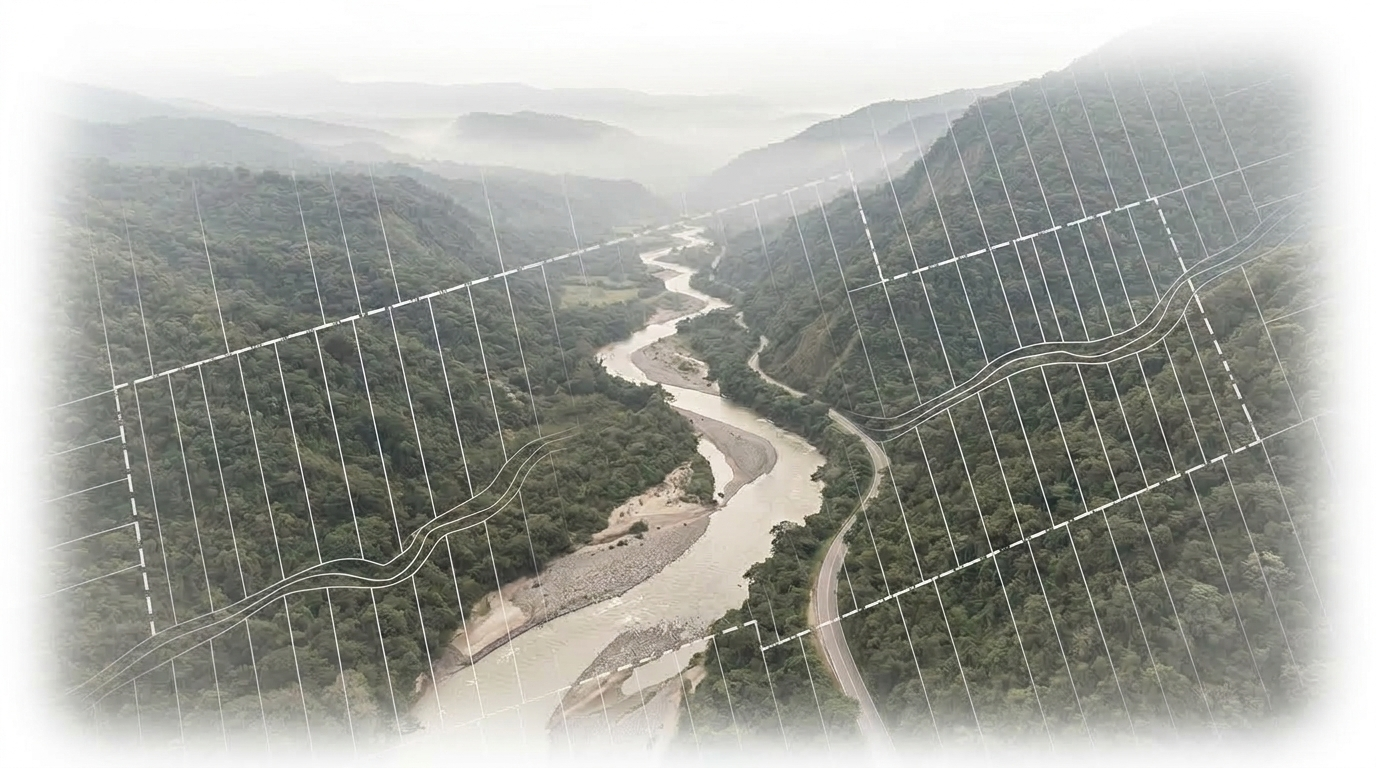
\includegraphics[width=\textwidth,height=6.8cm,keepaspectratio]{dispositivo-caldereño-2}
\end{center}

\vfill

{\color{tinta}\rule{\textwidth}{0.5pt}}
\vspace{8pt}

{\Large\scshape Eduardo Diedrich\par}
\vspace{4pt}
{\sffamily\footnotesize\color{gris}
Continuación territorial de \textit{El dispositivo salteño}\par}

\restoregeometry
\end{titlepage}

% --- página de créditos -------------------------------------------------
\thispagestyle{empty}
\null\vfill
{\footnotesize\color{gris}\setlength{\parskip}{0.6em}\parindent=0pt
\textbf{El dispositivo caldereño.} Dos circuitos de suelo y una capa fina en el
corredor norte del Valle de Lerma, 1908--2026.

Relevamiento documental sobre fuentes públicas: Boletín Oficial de la Provincia
de Salta desde su número 1 del 15 de octubre de 1908, normativa provincial y
municipal, censos nacionales y prensa. Los límites del trabajo, sus errores
corregidos y lo que no pudo verificarse están declarados en la Advertencia
preliminar y en el capítulo~\ref{cap:metodo}.

Este libro no contiene entrevistas propias. Las personas y sociedades que nombra
lo son en su carácter público y sobre la base de actos publicados; las
coincidencias de nombre se consignan como tales y no como identificaciones.

\textbf{La imagen de la portada} es una composición del autor ---un valle con una trama de
amanzanamiento superpuesta---: \textbf{no es una fotografía y no documenta un lugar
determinado}. Está fuera del índice de láminas y por eso no lleva epígrafe de procedencia;
su cadena de producción ---dibujo a mano, digitalización, \textsc{corel draw} y una pasada
de optimización con un modelo generativo de imagen--- la declaran la Advertencia preliminar
y el apéndice \ref{cap:fuentes}.

Compuesto en Charter. Composición del autor.\par}
\vspace{2em}
\cleardoublepage

\chapter*{Advertencia preliminar}
\addcontentsline{toc}{chapter}{Advertencia preliminar}
\markboth{Advertencia preliminar}{Advertencia preliminar}

Este libro continúa \textit{El dispositivo salteño} sobre un territorio de dos municipios. El apéndice E de aquel libro dejó cuatro hipótesis abiertas sobre el mercado inmobiliario como dimensión económica propia del dispositivo --- numeradas H.20 a H.23 --- y admitió que su documentación excedía lo que un autor sin infraestructura de investigación colectiva podía emprender. Este volumen no las confirma. Las lleva a una escala donde son verificables, y en el camino descubre que la hipótesis con la que empezaron era incorrecta.

Aquel apéndice suponía un mercado de suelo que opera contra un Estado ausente. Lo que este relevamiento encontró es otra cosa, y son dos.

La primera: dos regímenes estatales de producción de suelo que funcionan sobre el mismo territorio, con normas propias, organismos propios y poblaciones destinatarias distintas, y cuya diferencia central no es la legalidad sino la intensidad con que el Estado se ocupa de cada uno --- una intensidad inversamente proporcional a la capacidad de sus destinatarios.

La segunda apareció sola, por repetición, en el propio trabajo de conseguir los documentos: la opacidad de este territorio no está en el acto sino en el criterio. Seis instrumentos de dos niveles de gobierno ---el municipal y el provincial--- publican la envoltura y reservan a un anexo el contenido que permitiría verificar si alguien fue tratado con la misma vara que otro; otros ---al menos siete, cinco del régimen de tierra fiscal, uno de Recursos Hídricos y uno de Seguridad--- lo publican sólo como imagen escaneada, que ningún buscador encuentra. \textbf{Seis es lo que quedó de un inventario sistemático de trece ---depurado cuando ocho de sus casos resultaron publicados y ampliado con uno hallado al verificarlos---; no es el total}: cada documento incorporado después de cerrar ese recuento agregó casos de la misma especie, incluido el propio Código de Ordenamiento Territorial del municipio, que declara no urbanizables ambas márgenes del río y remite el ancho de esa franja a un plano que sólo se publica como imagen, sin escala que permita medirlo. Nada de ello es ilegal, y por eso funciona.

A esas dos se sumó una tercera cuando el relevamiento retrocedió hasta el primer número del Boletín Oficial, en 1908: las unidades territoriales, los nombres y las formas institucionales son los mismos desde hace más de un siglo. El mercado inmobiliario no construyó este dispositivo, lo encontró armado --- aunque no intacto, porque el municipio había perdido en el camino la voz que alguna vez tuvo sobre el agua de su jurisdicción.

Ninguna de las tres es una tesis sobre captura. El capítulo~\ref{cap:planteo} las enuncia, los capítulos~\ref{cap:fincas} y~\ref{cap:siglo} documentan la tercera y el~\ref{cap:opacidad} desarrolla la segunda.

Conviene contestar acá, y no en la página seiscientos, la pregunta que este material provoca
antes que ninguna otra: \textbf{si esto es una denuncia de corrupción}. No lo es, y el motivo no
es prudencia sino resultado. En todo lo relevado ---los años 1908 a 1921 del Boletín Oficial leídos hoja
por hoja, mil cuatrocientas noventa y dos ediciones entre 1923 y 1945, los años
1946 a 1950, un expediente judicial, dos códigos de ordenamiento y una década de
resoluciones--- \textbf{este libro no encontró un solo acto ilegal, ni un pago, ni una
instrucción, ni un acto dirigido a beneficiar a alguien con nombre}. Cada uno de los actos que
produce el resultado que el libro describe tiene su fundamento propio y su autoridad
competente.

Tampoco es la historia de un malentendido. Lo que hay es un conjunto de omisiones que, durante
más de un siglo, beneficiaron siempre al mismo lado: criterios que no se publican, líneas que se
publican dos días y no quedan asentadas en la matrícula, un municipio al que se le asignó
regular el suelo sin darle con qué, y una intensidad regulatoria que baja cuando sube la
capacidad del destinatario. \textbf{Ese resultado no necesita que nadie lo haya querido, y eso
es lo que lo vuelve difícil de corregir}: no se arregla encontrando a un culpable. El capítulo
\ref{cap:conclusion} lo dice al final con los documentos ya en la mano, y el
\ref{cap:prospectiva} explica por qué la palabra del título no equivale a conspiración ni a
accidente.

Cuatro advertencias sobre el registro.

\textbf{Primera.} La escala municipal agrava la exigencia metodológica en lugar de aliviarla. En un departamento de unos doce mil habitantes todos se conocen, y el costo de nombrar recae sobre personas identificables. La regla del libro anterior --- afirmaciones sobre posiciones estructurales, nunca sobre individuos morales --- rige aquí con más rigor. Un intendente que aprueba un loteo defectuoso no es, por ese hecho, un caso de corrupción; es, hasta que un expediente diga otra cosa, un caso de capacidad técnica insuficiente frente a una presión de mercado desproporcionada. El capítulo~\ref{cap:hacienda} muestra que esa lectura es, además, la correcta.

\textbf{Segunda.} Las cajas grises que aparecen a lo largo del texto marcan tipográficamente el punto exacto donde la exposición pasa de lo que consta en documento a lo que el autor infiere. Nada inferido sale de esa caja. Cuando una afirmación se apoya en prensa y no en instrumento público, se dice.

\textbf{Tercera.} \textbf{El estándar de cobertura de este libro no es uniforme, y conviene saberlo antes de leer cualquier afirmación sobre lo que falta.} Buena parte del Boletín Oficial se barrió por término de búsqueda sobre el texto extraído de los PDF, el período 1951--2012 sólo se consultó de manera puntual, y los años 1947 a 1950 se barrieron enteros pero sin lectura sobre la imagen (capítulo~\ref{cap:metodo}): ahí, que algo no aparezca significa solamente que el barrido no lo encontró. Hay treinta y dos tramos leídos edición por edición y verificados sobre la imagen ---de los treinta y seis que releva el apéndice \ref{cap:fuentes}, quedan fuera los cuatro de 1947 a 1950---, que forman dos ventanas: las \textbf{196 primeras ediciones del Boletín}, del número 1 del 15 de octubre de 1908 al 196 de octubre de 1910, a las que se suman \textbf{el resto de 1910 y los años 1911, 1912, 1913 y 1914 completos}; y las \textbf{mil quinientas tres} que van del número 962 al 2.464, junio de 1923 a diciembre de 1945 ---de las que quedan once sin leer, seis ausentes y cinco en blanco, que el apéndice \ref{cap:fuentes} enumera una por una: \textbf{mil cuatrocientas noventa y dos leídas}. A ellas se suman, al cierre, \textbf{el año 1946 completo} ---280 ediciones, del número 2.465 al 2.744--- y los años \textbf{1915} y \textbf{1916}, que en el momento de incorporarse eran el tramo más incompleto y el más limpio de la serie: 1915 con 49 ediciones de la 537 a la 586, sin la 581 y sin las de enero y la primera semana de febrero; 1916 con 49 ediciones de la 587 a la 635, sin un solo salto y con las 196 hojas presentes; \textbf{1917}, 47 ediciones de la 636 a la 683 sin la 640, 289 hojas de las 329 del año y sin OCR propio; \textbf{1918}, 52 ediciones de la 684 a la 736 ---falta entera la 703, que el repositorio reemplaza por un aviso de que no la encontró---, 534 hojas de los 587 folios del año, también sin OCR propio; \textbf{1919}, 49 ediciones de la 738 a la 786, 440 hojas de los 478 folios, con 38 hojas ausentes que caen todas al final de veintiocho ediciones y ninguna en el medio de ninguna; \textbf{1920}, 48 ediciones de la 788 a la 839 ---faltan cuatro: la 793, la 822, la 837 y la 838---, 526 hojas distintas y seiscientos folios; \textbf{1921}, 43 ediciones de la 840 a la 888 ---faltan seis---, 742 hojas y la cadena de folios del 1.681 al 2.532, que empalma sin hueco con el cierre de 1920; y \textbf{el primer semestre de 1922}, 27 ediciones de la 890 a la 916 y 446 hojas, del 13 de enero al 21 de julio, \textbf{único tramo que no cubre un año entero} ---de la edición 917 en adelante no hay archivo---, sin OCR propio, con un techo de resolución de 150 a 192 ppi, sin edición el viernes 14 de abril y con unas trece hojas ausentes dentro de las ediciones entregadas, que la cadena de folios detecta y el conteo de archivos no; y \textbf{1923 entero}, 52 ediciones de la 939 a la 990 y 673 hojas, una por cada viernes del año, sin un solo hueco en la serie ---el tramo más completo de la serie hasta que se incorporó 1924---, también sin OCR propio, con un techo de 150 ppi, con quince hojas que la cadena de folios declara ausentes hasta la edición 970 y con 322 hojas sin control de folio desde la 971, porque la numeración reinicia en cada edición; y \textbf{1924 entero}, 52 ediciones de la 991 a la 1042 y 792 hojas, \textbf{el primer año de toda la serie en que el calendario cierra solo} y en el que el cotejo entre el sumario y las páginas citadas cierra en las 52 ediciones; y \textbf{1925 entero}, 52 ediciones de la 1043 a la 1094 y 798 hojas, también sin huecos, con el control de paginación comprobado sobre veinticuatro hojas interiores y no sobre todas; y \textbf{1926 y 1927 enteros}, 52 ediciones cada uno ---1096 a 1147 y 1148 a 1199---, 769 y 745 hojas, las dos series semanales completas y sin huecos, con las cadenas de saldos incompletas y declaradas como tales; y \textbf{1928 entero}, 52 ediciones de la 1200 a la 1251, con dos meses sin resumen de Tesorería y con el salto de numeración de decretos más grande de la serie, del 7097 al 8001 en un solo día; y \textbf{1929, 1930, 1931 y 1932 enteros} ---ediciones 1252 a 1461---, los cuatro sin OCR propio, con un techo de 150 ppi, sin ninguna salida de barrido automático y \textbf{sin un solo plano publicado en los cuatro años}; y \textbf{1937 y 1938 enteros} ---ediciones 1669 a 1773---, el primer tramo en que los PDF traen capa de texto del proveedor: el 99\,\% de las hojas de 1937 no necesitó reconocimiento propio, y a cambio ese tramo no tiene confianza por hoja ni medición de tinta, lo que se declara como límite y no como pendiente; y \textbf{1939 y 1940 enteros}, con la misma capa y el mismo límite. Los años 1947 a 1950, barridos al cierre por pre-informe automático y sin lectura sobre la imagen, no forman parte de esas ventanas. En esas dos ventanas, y sólo ahí ---con la salvedad de los números y las páginas que faltan en cada una---, este libro puede afirmar que algo \textit{no está}. El apéndice \ref{cap:fuentes} detalla el método y enumera los ceros medidos.

\textbf{Cuarta.} Este relevamiento se equivocó más de una docena de veces, y \textbf{todas las correcciones
están incorporadas al cuerpo del texto en lugar de disimuladas}: se señala qué decía antes,
qué documento lo desmintió y qué dice ahora. Una fuente resultó pertenecer a otra provincia; una cláusula que parecía un vacío normativo resultó estar reglada en un instrumento que aún no se había leído; y un municipio que parecía carecer de reglamento de fraccionamiento resultó tenerlo sin publicar. Entre las restantes, dos merecen mención porque el libro las corrigió contra sí mismo: una fuente intermedia atribuyó a un acto administrativo cambios que su anexo original no contenía, y una observación sobre la unicidad de una omisión resultó falsa al ampliarse la serie. Se dejan asentadas porque describen el objeto: investigar sobre una normativa cuyos anexos no se publican produce, con regularidad, la apariencia de vacíos donde hay reglas, y trabajar con resúmenes en lugar de originales produce hallazgos que no existen.

El libro termina con tres piezas de naturaleza distinta, a las que se suma el capítulo prospectivo del que se habla más abajo. El capítulo~\ref{cap:conclusion} resume lo que el
relevamiento estableció y lo que no. El~\ref{cap:infraestructura} es una lectura del autor: relee lo documentado y agrega pocas piezas nuevas ---declaraciones vecinales, boletines municipales de la capital y un grupo de actos de 1935 a 1945 que sólo se desarrollan allí---,
y propone qué significa junto lo documentado. Y el~\ref{cap:plan} es, con el séptimo apéndice, lo único que este libro propone: qué habría que hacer, en qué orden y quién tendría que decidirlo. Los dos últimos van
marcados como tales, con sus condiciones de refutación, para que se los pueda discutir sin
discutir los documentos.

Los apéndices no son ilustración: son el aparato con el que se puede continuar o refutar
este trabajo. La cronología ordena los hechos desde 1690, con el grueso a partir de 1908; la matriz reúne los emprendimientos
con lo que se sabe y lo que no de cada uno; el inventario normativo transcribe lo que se pudo
obtener; el cuarto apéndice reúne, por organismo, todo lo que falta pedir; y el quinto reúne
a las personas que el archivo registra más de una vez, con la advertencia expresa de que son
coincidencias de nombre y no identificaciones. El sexto declara de qué clase de fuente sale
cada parte del libro, y qué clase de fuente no tuvo; y el octavo reconstruye, acto por acto, cómo circuló la tierra del departamento entre 1909 y 1945.

\textbf{Y hay un capítulo que mira hacia adelante, el \ref{cap:prospectiva}}, el único que proyecta ---el \ref{cap:plan} propone, pero no pronostica---: somete a prueba la palabra del título ---\textit{dispositivo}--- contra lo que los capítulos anteriores documentan, y de esa prueba deriva qué dinámicas están en curso. \textbf{Argumenta más de lo que documenta y lo dice al comenzar.} Quien quiera sólo lo verificable puede saltearlo sin perder nada de lo demás.

\textbf{Y un capítulo, el \ref{cap:ausencias}, hace lo mismo con el propio libro}: inventaría las dimensiones de la vida del departamento que este relevamiento no cubre ---la escuela, la salud, el comercio, el transporte, la iglesia, las mujeres---, reúne lo poco que el archivo dejó de cada una y dice qué haría falta. Está publicado a propósito, para que la lista de lo que falta sea pública antes de que exista el trabajo que la llene.

\textbf{Y hay un séptimo apéndice que es de otra naturaleza y conviene avisarlo acá.} Propone texto
normativo: seis ordenanzas, quince leyes y cinco actos del Ejecutivo, con su articulado. Nace
de una constatación del último capítulo --- que en los ocho puntos donde este territorio se
decide, nadie está obligado a nada --- y traduce cada uno de esos márgenes en un deber con
plazo. \textbf{Ninguna de las veintiséis propuestas manda decidir de un modo determinado}: mandan
publicar, fundar, registrar y cruzar. El apéndice aclara además que son borradores de
contenido y no de técnica legislativa, y que quien los tome deberá pasarlos por asesoría. 

Las cuarenta y una láminas tampoco son ilustración. Siete son facsímiles de cartografía, cuadros y notas oficiales que provienen de una misma pieza, el incidente de cumplimiento del amparo colectivo ---Expte.\ INC 23860/1--- que analiza el capítulo~\ref{cap:amparo}: tres mapas temáticos de la Secretaría de Recursos Hídricos de mayo de 2022, la hoja de firmas de ese informe, un cuadro de informes de impacto ambiental de canteras, la nota de la autoridad minera que lo acompaña y el Anexo I del atlas del Código de Ordenamiento Territorial. Ninguna de esas siete estaba publicada en un boletín ni en un portal público. Otras tres provienen de los documentos del Plan de Manejo: su tabla de costos y dos diapositivas de la presentación del Plan Maestro de Drenaje. Once salen de fuentes públicas de consulta difícil: el Anexo II del mismo atlas tal como lo publica el municipio, el plano de mensura 000962 y un detalle de su recuadro vial, cuatro capturas del visor cartográfico provincial, tres mapas de la red de gas del ENARGAS y el organigrama de un ministerio provincial publicado como anexo del Boletín. Las veinte restantes son de elaboración propia ---once mapas, el de ubicación del departamento, el de las fincas del archivo sobre el catastro vigente, el de la numeración de los planos de mensura, el de las líneas de ribera con coordenadas publicadas en los edictos, el de las líneas de ribera sobre el catastro, el de formación por radio censal, el del ordenamiento de bosques en el departamento, el del catastro que reclama la comunidad Kondorwaira, el de los actos de agua del departamento, el de dónde caen hoy los topónimos de 1909 a 1948 y el de las tres fracciones censales, y nueve gráficos: censo, padrón, caudales, la matriz de la toponimia en trece nóminas, la línea de tiempo de los cargos, la coparticipación municipal de 1947, las defensas contra crecientes de 1947 y 1949, la cobertura del Boletín Oficial que este libro leyó y lo que el Estado votó frente a lo que llegó--- y cada epígrafe dice con qué datos se hicieron y, en catorce de las veinte, con qué script: los scripts, las capas recortadas al departamento y las figuras están en el repositorio cartográfico \texttt{mapas\_caldera}, cuyo inventario detalla el apéndice \ref{cap:fuentes}. \textbf{Siete más tres más once más veinte son las cuarenta y una}, y el apéndice \ref{cap:fuentes} declara con qué se produjo cada una de las veinte propias, cuáles catorce son reproducibles por cualquiera ---script publicado, capas en un \textit{Release} y la cadena probada de punta a punta--- y cuáles seis no lo son todavía. \textbf{Se reproducen porque el argumento de
este libro sobre la opacidad se sostiene o cae en documentos como estos}, y el lector tiene
que poder mirarlos. El epígrafe de cada una dice de qué hoja salió; los retoques se limitaron a recortar márgenes, girar alguna hoja y ampliar un detalle, y cada epígrafe lo declara. Donde la reproducción no alcanza para medir --- y en
varias no alcanza --- se dice en el mismo lugar. \textbf{Y la imagen de cubierta no es una de las cuarenta y una}: es una composición del autor ---dibujo a mano, digitalización, \textsc{corel draw} y una pasada de optimización con un modelo generativo de imagen--- que enuncia el objeto del libro y no documenta nada. El apéndice \ref{cap:fuentes} lo declara con su cadena de producción, y deja constancia de que ninguna de las cuarenta y una láminas pasó por un modelo generativo.

Y hay algo que este relevamiento encontró tarde y que conviene saber desde el principio: \textbf{la zona alta de la cuenca es territorio de ocupación tradicional de una comunidad kolla}, relevado por el Estado nacional en 2011 y ratificado en 2023. Todo lo que este libro documenta ---los partidos de 1909, las fincas, los loteos--- se superpone a una capa anterior que el Boletín Oficial no registra.

Dos declaraciones de interés, que el cuerpo desarrolla donde corresponde y que conviene conocer desde aquí. La línea de investigación sobre la sociedad titular del loteo El Durazno llegó a este trabajo por encargo de un tercero interesado, con nombre puesto de antemano; se la siguió con los mismos estándares que al resto (capítulo~\ref{cap:loteo}). Y la consultora del sector Educación del plan estratégico provincial que el libro analiza es hermana del autor (capítulo~\ref{cap:trabajo}).\par\medskip El libro está cerrado como relevamiento documental y abierto como investigación. No contiene entrevistas propias: todo testimonio consignado proviene de prensa y se atribuye como tal, salvo dos conversaciones informales con vecinos, que el capítulo~\ref{cap:poblacion} registra como testimonio oral. Esa carencia se declara aquí, se retoma en el cierre y resulta ser --- según se argumenta allí --- la misma carencia que impide llevar la segunda tesis más lejos.

\tableofcontents
\cleardoublepage
\listoffigures
\mainmatter
\parte{El objeto}
{Qué se estudia, con qué fuentes y con qué límites. Las tres tesis del libro y las condiciones bajo las cuales cada una podría refutarse.}
\chapter{Las tres tesis}

\label{cap:planteo}
\section{Primera tesis: dos circuitos, regulación inversa}

En el departamento La Caldera operan dos circuitos de producción de suelo.

El primero es privado. Una parcela madre de gran superficie, generalmente de origen sucesorio o institucional, se estructura mediante fideicomiso o convenio, se desmonta, se mensura, se aprueba, se comercializa. Produce lotes de seiscientos metros cuadrados o más, para compradores de sectores medios y altos, en el lapso de un ciclo comercial.

El segundo es estatal. La Provincia adjudica tierra fiscal a familias de bajos ingresos, por sorteo público o por regularización de ocupaciones consolidadas, con un régimen de inscripción, puntaje, tenencia precaria y adjudicación en venta financiada. Produce lotes de interés social en plazos que, en los casos documentados, se miden en años y, en algún caso, en décadas: en un barrio de la capital en el que, según su centro vecinal, se adjudicaron lotes a vecinos del departamento, hay un expediente iniciado en 1995 y resuelto en 2025.

Los dos circuitos están regulados en proporción inversa a la capacidad de sus destinatarios. Al solicitante de un lote fiscal se le exige certificado policial de residencia, declaración jurada bajo pena de falso testimonio, referencias vecinales con nombre y apellido, franja horaria de visita domiciliaria, informe socioambiental y construcción en tres meses bajo apercibimiento de revocación. Al desarrollador que convierte monte de yungas en doscientas cuarenta y siete parcelas sobre una microcuenca judicialmente condenada se le exigen, en el papel, diez actos municipales ---los que enumera el Código de Ordenamiento (capítulo \ref{cap:cot})--- y, entre ellos y los provinciales, dos que aquí importan: un certificado de aptitud ambiental municipal y un \textbf{Certificado de No Inundabilidad} que la reglamentación del Código de Aguas califica de \textbf{recaudo indispensable} para todo loteo cuyo límite sea un río. \textbf{Ninguno de los dos aparece nombrado en el acto que aprobó el loteo más discutido del departamento}, y en el resto de los expedientes relevados sólo consta el de no inundabilidad, una vez, junto a un certificado ambiental provincial ---no el municipal---, en la respuesta de un loteador a una intimación municipal (capítulo \ref{cap:amparo}).

No se trata de un régimen laxo que favorece la discrecionalidad. Se trata de un régimen exigente aplicado a quien menos tiene y de un régimen tenue aplicado a quien más puede, sobre suelo del mismo corredor y bajo la misma autoridad provincial.

\section{Segunda tesis: la opacidad está en el criterio, no en el acto}

La segunda tesis no formaba parte del proyecto. Se impuso al cabo del relevamiento, cuando el mismo obstáculo apareció cinco veces seguidas en instrumentos de dos niveles de gobierno distintos, el municipal y el provincial.

La Ordenanza 437 de Vaqueros aprueba el Reglamento de Fraccionamiento de Tierras; el reglamento va en un anexo que el Boletín Oficial no publicó. La Resolución 82/16 aprueba el Reglamento de Asignación de Lotes de Interés Social y a él se remite el plazo de exhibición de los padrones; el reglamento va en un anexo que el Boletín sólo ofrece como imagen escaneada, que ningún buscador encuentra. La Resolución 8/16 establece el sistema de puntaje por vulnerabilidad social; el baremo va en un anexo que también se publica sólo como imagen. La Resolución 9/16 regula el sorteo público y su publicidad; el procedimiento va en otro anexo publicado del mismo modo. El Decreto 63/25 adjudica ciento tres parcelas conforme a un anexo que se publica aparte, como archivo vinculado, y que después se corrige por una resolución que subsana errores materiales.

El acto se publica. El criterio no se publica, o se publica de un modo que nadie lo encuentra: cuatro de esos cinco anexos resultaron estar en el repositorio del Boletín ---tres de ellos como imágenes escaneadas, sin texto que un buscador pueda leer---, y el quinto, el reglamento de Vaqueros, que el Boletín nunca publicó, apareció al final en el digesto en línea del propio municipio (capítulo \ref{cap:vaqueros}).

A eso se suma un mecanismo distinto y complementario. El Código de Ordenamiento Territorial de La Caldera declara sectores no urbanizables y, a continuación, prevé la figura del Proyecto Especial que permite urbanizarlos con más pasos. El proyecto de ordenanza del Plan de Desarrollo Urbano Ambiental emplea la fórmula ``quedará a consideración del municipio'' seis veces sin definir qué debe considerarse, con qué dictamen ni en qué plazo. La calificación de no urbanizable no opera como prohibición: opera como requisito de procedimiento agravado.

Ninguna de estas prácticas es ilegal. Los anexos existen, integran los actos y son accesibles por pedido; la excepción está prevista en la norma y se tramita conforme a ella. Y precisamente por eso el resultado es más eficaz que cualquier ocultamiento: no deja nada que denunciar.

El capítulo \ref{cap:opacidad} desarrolla esta tesis con el inventario completo. Se anuncia aquí porque el lector la va a encontrar antes, dispersa, en cada capítulo donde el libro se acerca a una decisión y encuentra publicada la envoltura y reservado el contenido.

\section{Tercera tesis: el dispositivo es anterior al mercado}

La tercera apareció como la segunda: por acumulación, y ya avanzado el trabajo. Surgió al
retroceder el relevamiento hasta el primer número del Boletín Oficial, en 1908.

Las unidades territoriales sobre las que hoy se lotea son las divisiones administrativas
del departamento a comienzos del siglo XX. Varios de los trece partidos policiales de 1909 —San Alejo, Los Porongos, Potrero de Gallinato, Potrero de Castillo, La Calderilla, Los Yacones— llevan los nombres de fincas y parajes que el proyecto de ordenanza del plan urbano de 2015 enumera como integrantes del municipio ---este libro leyó el proyecto, no el texto sancionado (capítulo \ref{cap:pdua})---; otros —Lesser, Vaqueros— nombran hoy parajes, cursos de agua o un municipio entero; y una fracción de Los Porongos es una de las que una ley de 1972 declaró afectadas. La finca Potrero de
Gallinato es partido en 1909, se remata judicialmente en 1922, la Provincia adquiere una
fracción por prescripción en 2015 y ese mismo año se aprueba sobre ella un club de campo de
mil quinientas sesenta y nueve hectáreas. La finca Cerro de Buena Vista se deslinda ante un
juez en 1921, obtiene agua en 1924 y llega a audiencia pública ambiental como urbanización
en 2014.

Lo mismo vale para las formas institucionales. La Caldera es una Comisión Municipal con
presidente designado por el gobernador en 1908, lo sigue siendo en 1922 —cuando el
Interventor Nacional nombra a sus cinco miembros y el Poder Ejecutivo le aprueba el
presupuesto— y todavía en 1983, en vísperas del traspaso democrático. En 2022 sigue
clasificada en la tercera categoría, como Vaqueros, que ya tiene población de segunda: La Caldera conserva la categoría que un decreto le fijó en 1931 y Vaqueros la que su ley de creación le dio en 1970, en un departamento de doce mil trescientos habitantes.

Y lo mismo vale para el problema del río. En enero de 1910 los vecinos del pueblo pidieron
al gobierno que se los defendiera «de las invasiones del Río del mismo nombre», y la
Provincia asignó fondos, nombró una comisión y le pidió al municipio que cofinanciara. En
febrero de 2026, diez días antes de que una jueza aprobara un plan de manejo, el municipio
informaba que construía bateas y muros de contención con maquinaria pesada.

De ahí la tercera tesis:

\begin{quote}
El dispositivo no se construyó para el mercado inmobiliario. El mercado inmobiliario
encontró un dispositivo ya armado —unidades, nombres, formas institucionales, obras de
defensa y opacidad dominial— y lo usó. Lo que cambió en el último cuarto de siglo no es el
territorio ni su administración: es el uso al que se destina el suelo.
\end{quote}

Esta tesis no reemplaza a las otras dos: las fecha. La regulación inversa y la opacidad del
criterio no son innovaciones de los años dos mil. Son formas antiguas de administrar un
territorio, que un ciclo inmobiliario reciente puso a trabajar en otra escala.

\subsection*{Lo que la tercera tesis no dice}

Formulada así, esa tesis describe una continuidad, y hay un punto en que el archivo la
contradice. Conviene decirlo aquí y no esconderlo en un capítulo interior, porque es la
objeción más seria que este libro se hace a sí mismo.

\textbf{En materia de agua, el municipio tuvo más poder en 1939 que en 2015.}

En 1914 el municipio de La Caldera dictó una ordenanza que reglamentaba la distribución de
\textbf{la totalidad} del caudal del río Santa Rufina, reconociendo derechos adquiridos por
uso tradicional. En 1939, al resolver el pedido que un comerciante de la capital había presentado en 1937 para obtener concesión sobre ese río
para regar la finca Campo Alegre, la Provincia \textbf{denegó} el pedido: hubo disenso
municipal, tres oposiciones de particulares, y el Poder Ejecutivo reconoció que otorgarla
alteraría el reparto fijado por aquella ordenanza. Al año siguiente confirmó la negativa
diciendo que \textbf{razones de orden legal le impedían} conceder agua de ese río.

Compárese con lo que el capítulo \ref{cap:ribera} documenta. Entre 2013 y 2015 la Secretaría de Recursos
Hídricos dictó veinticinco actos de línea de ribera sobre la cuenca del departamento, y en ninguno consta intervención municipal; la excepción, que la serie cuenta aparte, es la Resolución 023/14, dictada en 2014 a pedido del intendente sobre la ribera del propio pueblo. El capítulo \ref{cap:loteo} documenta que el plano de un loteo se
aprobó por resolución ministerial sin que figure ninguno de los diez actos que el
propio Código del municipio exige (apéndice \ref{cap:matriz}).

\textbf{Eso no es continuidad: es pérdida.} Y obliga a precisar la tesis en lugar de
abandonarla.

Lo que se mantiene idéntico durante un siglo son las \textbf{unidades} --- las fincas, los
nombres, los límites --- y la \textbf{forma institucional} del municipio: comisión de tercera
categoría, presidente designado, presupuesto aprobado desde afuera, renta que no alcanza. Lo
que cambió, y cambió en contra, es la \textbf{capacidad de decidir sobre los recursos de su
propio territorio}.

La tercera tesis queda entonces así:

\begin{quote}
El mercado inmobiliario encontró armado un dispositivo de unidades, nombres y formas
institucionales anterior a él. Pero no lo encontró intacto: encontró un municipio que había
perdido, en el camino, la voz que alguna vez tuvo sobre el agua y el suelo de su
jurisdicción.
\end{quote}

Cuándo y cómo se produjo esa pérdida es la pregunta que este libro no puede contestar del
todo, pero de la que tiene el punto de partida y una pista sobre el mecanismo. El punto de
partida documentado para La Caldera está en 1885: el capítulo \ref{cap:redes} documenta que en junio de ese año la Municipalidad de
La Caldera \textbf{concedió} treinta litros por segundo del río Wierna, y que el Estado
provincial reconoció esa facultad como legítima. El del mecanismo es anterior: en 1866 una ordenanza municipal de Campo Santo repartía el agua del Mojotoro y la Legislatura la sancionó como ley al año siguiente. La pista está en 1942, cuando ese mismo
derecho se \textbf{inscribe en los registros provinciales} y deja de constar en un acuerdo
municipal. \textbf{Y hay ahora un punto intermedio, que el barrido de 1918 aportó al cierre}: en
septiembre y en noviembre de ese año, dos decretos del Interventor Nacional nombran los Jueces de
Agua de los distritos de Caldera y de La Calderilla «\textit{vista la nota que antecede del Sr.\
Comisionado Municipal de Caldera, proponiendo \ldots\ las personas}» (capítulo
\ref{cap:siglo}). \textbf{La facultad municipal ya no es conceder: es proponer, y la firma es
provincial.} Conceder en 1885, proponer en 1918, inscribir en la provincia en 1942: la pérdida
tiene tres tiempos y el del medio recién aparece. El resto ocurre en los sesenta y dos años que el relevamiento no leyó de corrido ---y 1948 agrega un quinto tiempo, el más bajo: colaborar a pedido del organismo provincial (capítulo \ref{cap:siglo})---. El
capítulo \ref{cap:metodo} declara ese hueco entre los límites del trabajo, y el apéndice \ref{cap:pedidos} indica dónde
empezar a llenarlo.

\subsection*{Cómo se relacionan}

Las tres tesis describen el mismo objeto desde ángulos distintos, y conviene no confundirlas. Las dos primeras son sincrónicas: dicen cómo funciona el dispositivo. La tercera es de duración: dice desde cuándo.

La primera es sobre \textbf{a quién} se le exige. La segunda es sobre \textbf{qué se puede saber}. Y se articulan en un punto preciso: el solicitante de un lote fiscal tiene un baremo que lo mide, pero no puede consultarlo; el comprador de un lote privado tiene un reglamento que debería protegerlo, pero no puede leerlo. La opacidad no protege a los dos por igual, porque quien tiene abogado, tiempo y capacidad de gestión consigue el anexo, y quien no los tiene, no.

De modo que la segunda tesis no es un tema aparte: es el mecanismo por el cual la primera se sostiene sin que nadie tenga que decidirla.

\subsection*{Qué refutaría cada tesis}

Una tesis que no dice qué la desmentiría no se puede discutir: sólo se puede creer o no. Las tres se exponen aquí a la misma prueba que el libro aplica a cada expediente, con el documento que la resolvería y el lugar del apéndice \ref{cap:pedidos} donde ya está pedido.

\textbf{La primera tesis se cae si el circuito privado cumplió, en expediente, exigencias equivalentes a las del fiscal.} Su evidencia primaria es la Resolución 646D/21 frente a las Resoluciones 7, 8 y 9 de 2016 y al Anexo de la 82/16 (capítulos \ref{cap:loteo} y \ref{cap:tierrafiscal}). Si las fojas 58, 59, 68, 84, 97/101 y 137 del expediente 18-37.348/2019-0 contienen los certificados de no inundabilidad y de aptitud ambiental, la provisión efectiva de servicios y el visado hídrico que el anexo del Decreto 1682/19 exige, y si el registro de la Unidad Coordinadora muestra lo mismo para los demás loteos del corredor, la regulación no fue inversa: fue igual de exigente y este libro no la vio. Se cae también, por el otro extremo, si las actas de los sorteos y el registro público de tenedores precarios del artículo 1º inciso g de la Resolución 82/16 muestran que las exigencias escritas para el solicitante de tierra fiscal no se aplican en la práctica. Las dos series están pedidas a Inmuebles, al Boletín Oficial y a la Secretaría de Tierras y Bienes del Estado.

\textbf{La segunda tesis se cae si el criterio sí está escrito en algún lugar accesible.} Su evidencia primaria son los seis instrumentos del capítulo \ref{cap:opacidad} y los dos edictos de 2014 sobre la misma matrícula, uno con ciento trece pares de coordenadas y otro sin ninguno (capítulo \ref{cap:ribera}). Si la Secretaría de Recursos Hídricos tiene una resolución o instructivo publicado que fije cuándo se publican las coordenadas y cuándo no, o si los cinco anexos que no se obtuvieron se entregan a simple pedido, sin arancel y en plazo, y resultan no contener nada que decida ---ni obras exigidas, ni exenciones, ni puntos de ribera---, la opacidad es un defecto de infraestructura documental y no una forma de reservar el criterio. Los pedidos están en las secciones de Recursos Hídricos, del Boletín Oficial y de obra pública.

\textbf{La tercera tesis se cae si las unidades de hoy no descienden de las de 1909, o si el municipio recuperó la voz que perdió.} Su evidencia primaria son los deslindes de 1921 y 1932, el padrón de parajes de 1940, el revalúo de 1944 y la serie de 1885 a 1942 sobre el agua (capítulos \ref{cap:fincas}, \ref{cap:siglo} y \ref{cap:redes}). Si el antecedente dominial de las matrículas 4366 y 6.558 ---y de las demás matrículas de los loteos--- muestra que proceden de reagrupamientos posteriores y no de las fincas históricas, la continuidad de las unidades es sólo de nombres. Y si entre 1947 y 2012 ---el tramo que el relevamiento no leyó sobre la imagen: 1947 a 1950 sólo se barrieron, y de 1951 en adelante hubo consultas puntuales--- aparece un acto que devuelva al municipio competencia efectiva sobre el agua o el suelo de su jurisdicción, la «pérdida» que la tesis describe no es una pérdida sino una oscilación. Los folios y la serie de actos están pedidos a Inmuebles y al archivo provincial.

Ninguna de las tres condiciones se cumplió al cierre de este manuscrito. Ninguna fue puesta a prueba del todo: los documentos que las resolverían están pedidos y siguen sin obtenerse.

\section{Por qué este departamento y no otro}

La lámina \ref{fig:ubicacion} sitúa el departamento: el valle del río La Caldera baja de norte a
sur entre el dique Campo Alegre y Vaqueros, con la ruta nacional 9 como eje, y Vaqueros toca la
planta urbana del Gran Salta. Al oeste, las cumbres pasan de los cinco mil metros.

\begin{figure}[p]
\centering
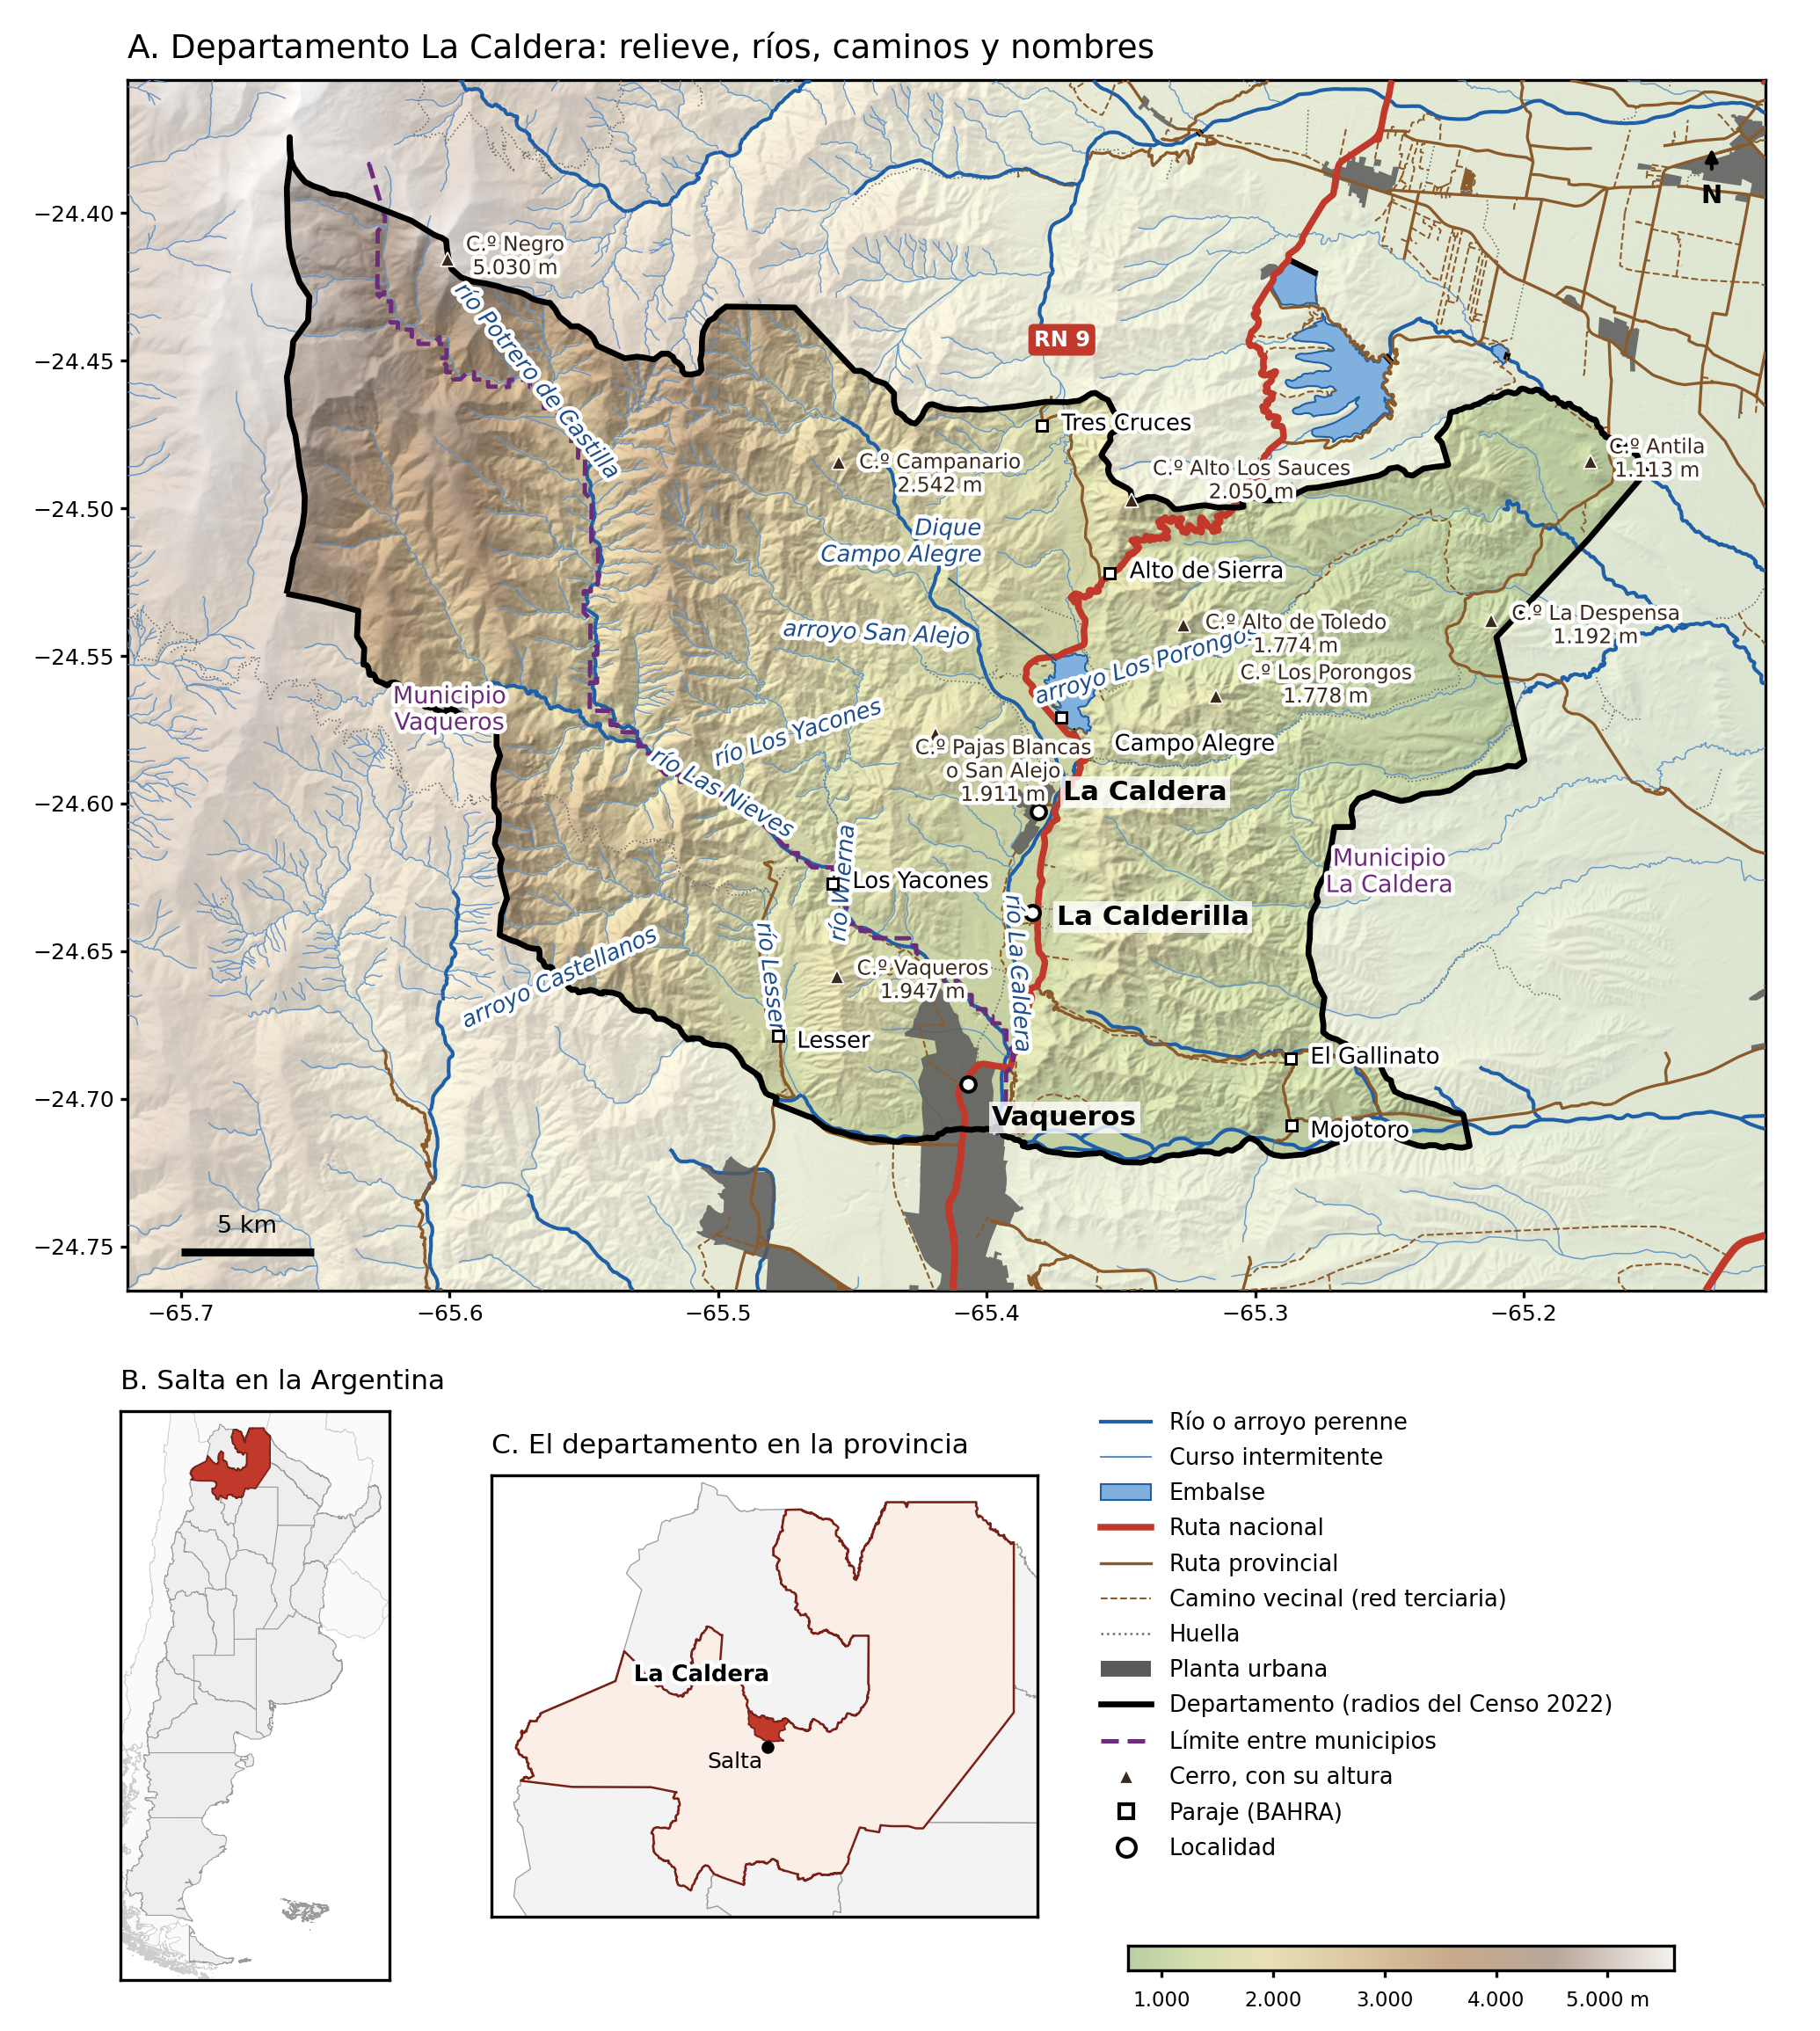
\includegraphics[width=\textwidth,height=0.84\textheight,keepaspectratio]{fig-ubicacion.png}
\caption[El departamento La Caldera]{\textbf{El departamento La Caldera.} A: relieve, ríos, caminos, localidades y cerros del departamento, con el límite entre los municipios de La Caldera y Vaqueros y los parajes que registra la Base de Asentamientos Humanos (BAHRA). B y C: ubicación de la provincia en la Argentina y del departamento en la provincia. Elaboración propia con el Modelo Digital de Elevaciones MDE-Ar v2.1 de 30 metros y las capas SIG del Instituto Geográfico Nacional (hidrografía, red vial nacional, provincial y terciaria, huellas, municipios, plantas urbanas y cerros), la BAHRA, la cartografía de radios del Censo 2022 (INDEC) y los límites de la plantilla oficial del IGN para la Argentina parte continental americana. Elaboración propia; dibujo de \texttt{scripts/mapa\_ubicacion.py} del repositorio \texttt{mapas\_caldera} (apéndice \ref{cap:fuentes}).}\label{fig:ubicacion}
\end{figure}

\textbf{Primero: es la frontera, no el destino.} San Lorenzo es donde el patriciado salteño ya vive; La Caldera y Vaqueros son donde el mercado está \textit{produciendo} suelo urbano ahora. El proceso completo --- desmonte, apertura de camino, mensura, aprobación, escritura, preventa --- es observable en tiempo presente y con litigio activo.

\textbf{Segundo: es la cabecera hídrica de la capital, y lo es por expropiación.} En junio de 1972 un gobierno de facto declaró de utilidad pública seiscientas ochenta y seis hectáreas del departamento para construir el embalse Campo Alegre, con compensación fijada en valuación fiscal más treinta por ciento y toma de posesión previa a la discusión del precio. El acueducto que hoy lleva esa agua a la cisterna El Huaico recorre unos veinte kilómetros atravesando ambos municipios. La microcuenca cuyo bosque se remueve para lotear es la zona de recarga del sistema que abastece a la ciudad. El capítulo \ref{cap:expropiacion} reconstruye esa expropiación y la propone como punto de partida de todo lo demás.

\textbf{Tercero: hay expediente.} Existe una causa judicial --- CUIJ 17-00023860-0 --- que reúne en una sola pieza al municipio que autoriza, la provincia que omite, el desarrollador que ejecuta y los vecinos que pierden. Ninguna reconstrucción sociológica externa habría producido un material comparable al que produjeron las propias partes al defenderse.

\textbf{Cuarto: es la escala del fenómeno.} Entre 2010 y 2022 el departamento creció un 58,4 por ciento y fue el cuarto de mayor crecimiento demográfico de la Argentina, detrás de dos partidos del conurbano bonaerense y de Añelo, la capital de Vaca Muerta ---ordenamiento verificado sobre los resultados definitivos de veintitrés de las veinticuatro jurisdicciones, con la reserva que precisa el capítulo \ref{cap:poblacion}---. Lo administran dos municipios clasificados en tercera categoría.

\section{Las hipótesis heredadas y su saldo}

Del apéndice E de \textit{El dispositivo salteño}, retomadas aquí como programa:

\begin{description}[leftmargin=2.2cm,style=nextline]
\item[H.20] El mercado inmobiliario opera como mecanismo simultáneo de blanqueo de rentas no declaradas, consolidación intergeneracional de patrimonio y segregación residencial.
\item[H.21] Existe correlación entre ciclos de renta extractiva extraordinaria y desarrollo de emprendimientos de alta gama.
\item[H.22] Los apellidos que desarrollan y titularizan los emprendimientos se solapan con los documentados en el cuerpo principal del libro anterior.
\item[H.23] La cooperación entre escribanías, inmobiliarias y estudios jurídicos permite estructurar operaciones que no tributan como inversión sino como adquisición patrimonial.
\end{description}

Al cierre del relevamiento, el balance de estas cuatro hipótesis figura en el capítulo \ref{cap:conclusion}. Se adelanta lo principal: \textbf{la hipótesis del blanqueo, que motivó el proyecto, no encontró un solo elemento de prueba.}

\begin{cautela}
Ese saldo es magro y conviene declararlo de entrada. Un libro que se propuso verificar cuatro hipótesis y verifica, a lo sumo, dos en parte podría presentarse como fracaso. Lo que ocurrió, en cambio, es que el material desplazó el objeto dos veces: la pregunta por el blanqueo no encontró evidencia; la pregunta por la asimetría regulatoria, que nadie había formulado, encontró toda la que necesitaba; y la pregunta por la opacidad apareció sola, por repetición, en el propio trabajo de conseguir los documentos.

Se deja constancia porque es el modo honesto de exponer una investigación que cambió de tesis mientras se hacía.
\end{cautela}

\chapter{Método, fuentes y límites}

\label{cap:metodo}
\section{Los tres registros}

El libro distingue tipográficamente tres niveles y no los mezcla. \textbf{Documento}: sentencias, ordenanzas, decretos, resoluciones, boletines oficiales, expedientes administrativos, publicaciones institucionales. Se cita con identificación completa. \textbf{Prensa}: cobertura periodística verificable, con medio y fecha, consignada siempre como afirmación del medio y no como hecho establecido. \textbf{Inferencia del autor}: va en caja gris, nunca fuera de ella.

\section{El corpus}

\textbf{Judicial.} La causa \textit{Lazarte Vigabriel y otros c/ Municipalidad de La Caldera; Ministerio de la Producción, Trabajo y Desarrollo Sustentable --- Amparo Colectivo} (CUIJ 17-00023860-0; piezas pertenecientes INC 23860; incidente INC 23860/1; ejecución, Expte.\ 780280), ante el Juzgado de Minas y en lo Comercial de Registro del Distrito Judicial Centro, es la columna vertebral del libro.

\textbf{Sobre la numeración del expediente principal hay una discrepancia que este libro no resuelve.} Una providencia de agosto de 2022 lo identifica como \textbf{MIN 23860/19}; otras piezas del corpus lo consignan como \textbf{EMI 23860/2020}. Ambas formas se conservan tal como aparecen en sus fuentes. Esa misma providencia deja constancia de que en 2022 el expediente principal \textbf{se encontraba radicado ante la Corte de Justicia de la Provincia}, razón por la cual la etapa de cumplimiento se tramitó en piezas separadas.

Conviene anotar que \textbf{la sentencia la dicta el Juzgado de Minas} y que la etapa de cumplimiento tramita en piezas separadas, con carátula de amparo colectivo y numeración propia (INC 23860/1 y 780280); el capítulo \ref{cap:amparo} explica esa relación. Su contenido se reconstruye aquí a partir de la ficha del caso elaborada por el Observatorio Argentino de Litigación Climática de la Universidad Nacional del Litoral, de los partes de prensa del Poder Judicial de Salta y de la consulta al sistema de expediente digital; el texto íntegro de la sentencia no fue consultado, y ésa es la principal debilidad documental de este libro. \textbf{La única transcripción disponible es parcial y la eligió el propio obligado}: el informe que la Provincia presentó en 2022 cita «la parte pertinente» de los mandatos que debía cumplir --- del punto VII sólo el inciso a) y sólo su primer párrafo ---, y su estructura sugiere que hay al menos cuatro mandatos más cuyo texto no consta. Se le suman el amparo por la cuenca del río Mojotoro de 2019, el amparo rechazado contra la Municipalidad de Vaqueros por el loteo \textit{Lares de la Inmaculada}, y como caso comparado el peritaje sobre el barrio privado \textit{Los Maitines} en San Lorenzo.

\textbf{Normativo.} Se obtuvo y leyó el texto operativo de: el Código de Ordenamiento Territorial de La Caldera (152 artículos, ocho anexos, atlas de ocho planos); el Informe Final y el Proyecto de Ordenanza del Plan de Desarrollo Urbano Ambiental que ese Código reglamenta; el Código de Planeamiento Urbano Ambiental de Vaqueros en su texto de 2026; la Ley 2616 de 1951; el Decreto 399/20 de creación del Plan ``Mi Lote''; las Resoluciones 82/16 y 86/16 del Ministerio y 7/16, 8/16 y 9/16 de la Secretaría de Tierra y Bienes, con los anexos de la 82/16, la 7/16, la 8/16 y la 9/16 ---copias certificadas que el repositorio del Boletín ofrece sólo como imagen---; el Decreto 4.414/08 que encabeza esa cadena; los decretos de designación 120/15 y 64/23; el Decreto 844/21 de traslado orgánico; el Decreto 63/25 de adjudicación y su anexo nominal.

\textbf{Cómo se transcribe.} Las citas de documentos reproducen el texto del original, con dos
convenciones declaradas. \textbf{Se moderniza la acentuación} ---el Boletín histórico
imprime «Nacion», «rio», «hectàreas», «areas»; los ejemplos son de 1908 a 1912, y la
convención rige para todo el corpus anterior a 1947--- y \textbf{se unen las palabras partidas por el
corte de renglón}, porque ni una cosa ni la otra pertenecen al texto sino a la imprenta. En
cambio \textbf{las erratas de palabra se conservan tal cual, con \textit{[sic]}}: así van «el
Augosto de Arias» junto a «el Angosto de Arrieta» en el mismo decreto de 1912, «Rejis» por
«Regis», «Depto. de la Caldera» y las dos superficies distintas de una misma finca en un mismo
aviso. Donde el original se contradice, se transcriben las dos formas y no se elige.

\textbf{Histórico.} El archivo digital del Boletín Oficial de la Provincia, desde su número 1 del 15 de octubre de 1908. Se leyeron \textbf{edición por edición} treinta y seis tramos, que el apéndice \ref{cap:fuentes} detalla uno por uno con sus ausencias de edición y de hoja: las 196 primeras ediciones, de octubre de 1908 a octubre de 1910; los años \textbf{1911 a 1921} completos, del número 220 al 888; el \textbf{primer semestre de 1922}, del 890 al 916, que es hasta donde llega el repositorio ---de la edición 917 en adelante no hay PDF---; los años \textbf{1923 a 1932} completos, del 939 al 1.461; las ediciones que van del número 962 al 2.464, de junio de 1923 a diciembre de 1945, de las que faltan treinta y una; y, al cierre, los años \textbf{1937 a 1946} completos, hasta el número 2.744, y \textbf{1947 a 1950}, de la edición 2.869 en adelante, estos cuatro con barrido automático y \textbf{sin lectura sobre la imagen}, según declara el apéndice \ref{cap:fuentes}. Se barrió además por término de búsqueda el período 2013--2015, y de manera puntual el resto. El apéndice \ref{cap:fuentes} detalla el método. De ese corpus provienen los partidos policiales de 1909 y 1911, los decretos de defensa contra el río de 1910 y 1911, las rendiciones municipales de 1908 y 1922, los pedimentos mineros de 1908 y 1925, los deslindes de 1910 y 1921, la concesión de agua de 1924, la fundición de Mojotoro y el racionamiento del Wierna de 1946.

\textbf{Hemerográfico.} La cronología del apéndice \ref{cap:cronologia} reúne el barrido 2015--2026. Los medios con cobertura sostenida del proceso son \textit{Página/12} en su edición salteña, \textit{El Tribuno}, \textit{Cuarto Poder}, \textit{Que Pasa Salta}, \textit{Cuarto}, \textit{Nuevo Diario de Salta} y \textit{Salta 4400}.

\textbf{Académico.} Literatura sobre Vaqueros como caso de transformación periurbana; trabajo sobre urbanización de la pobreza en el aglomerado Gran Salta; y un relevamiento de la universidad confesional provincial que identificó, para Salta capital y municipios vecinos, cinco urbanizaciones privadas y once clubes de campo aprobados por la Dirección General de Inmuebles, frente a cincuenta y cuatro asentamientos.

\begin{cautela}
Ese contraste --- dieciséis urbanizaciones cerradas contra cincuenta y cuatro asentamientos en el mismo aglomerado --- es el marco de todo el libro. No hay un mercado de suelo que crece: hay dos mercados que crecen en paralelo, con regímenes jurídicos, ritmos de provisión de servicios y capacidades de gestión radicalmente distintos, sobre el mismo aglomerado.
\end{cautela}

\section{Un sesgo de la fuente que terminó siendo un hallazgo}

El obstáculo apareció primero en cinco instrumentos: el Reglamento de Fraccionamiento de Tierras de Vaqueros (Ordenanza 437), la nómina de adjudicatarios del Decreto 63/25, el baremo de puntaje de la Resolución 8/16, los procedimientos de sorteo de la Resolución 9/16 y el Reglamento de Asignación de la Resolución 82/16.

Al ampliarse el relevamiento la lista creció. Se sumaron el contrato de promoción turística que ratifica el Decreto 3069/14, con el detalle de las exenciones concedidas; las coordenadas de dos determinaciones de línea de ribera, remitidas a la sede del organismo; y el informe técnico que funda la contratación por vía abreviada del Plan de Manejo.

Con los que se agregaron después ---el anexo del Decreto 1682/19, el de la Resolución 023/14, los de la Resolución 567D/26 y el convenio del Decreto 1433/15--- la lista llegó a trece. De los trece, \textbf{ocho resultaron estar publicados} como archivos vinculados en la edición web del Boletín ---la nómina del Decreto 63/25, el reglamento de la Resolución 82/16, los anexos de las Resoluciones 8/16 y 9/16 y los cuatro que se sumaron al final---, varios de ellos sólo como imagen escaneada; los \textbf{cinco restantes} siguen fuera, contando por separado las dos determinaciones de línea de ribera. El capítulo \ref{cap:opacidad} da la lista definitiva ---seis instrumentos, de los que al final del trabajo se obtuvo uno, el reglamento de Vaqueros---, que son esos cinco ---la Ordenanza 437, las Resoluciones 142/14 y 383/14, el Decreto 3069/14 y el informe técnico del Plan de Manejo--- más el Decreto 463/15, hallado al verificarlos.

Los anexos no son secretos: existen, integran los actos y son accesibles por pedido. Pero contienen, sin excepción, el contenido decisorio --- qué obras debe hacer un loteador, cuántos puntos vale una discapacidad, cuántos días tiene un vecino para impugnar un padrón --- mientras la parte publicada contiene la envoltura. Quien insiste los consigue; quien lee el Boletín Oficial de buena fe como texto, no: varios de ellos sólo existen allí como imagen.

Este apartado se escribió, en una primera versión, como una advertencia práctica para quien continuara la investigación. La repetición del obstáculo lo convirtió en objeto: el capítulo \ref{cap:opacidad} lo retoma como segunda tesis del libro.

\begin{cautela}
Esto tiene una consecuencia metodológica que el libro debió aprender por error. Trabajar sobre una norma sin su anexo produce la impresión de un vacío donde hay una regla. Este relevamiento afirmó, en una etapa intermedia, que la asignación directa de lotes fiscales era una excepción admitida sin reglamentar; al obtener el anexo faltante resultó ser una de las cláusulas mejor acotadas del régimen, con destinatario definido, informe fundado, doble firma, período de tachas y tope del dos por ciento.

La regla que se sigue de aquí en adelante, y que se recomienda a quien continúe: ninguna afirmación sobre ausencia de norma sin haber agotado la cadena de remisiones.
\end{cautela}

\section{Una trampa de homonimia}

Durante el relevamiento apareció un sitio de noticias con dominio \texttt{lacaldera.com.ar}, con secciones de política y judiciales, que publica notas sobre el Partido Justicialista, denuncias de aprietes a intendentes y licitaciones sospechosas, y una nota de junio de 2025 sobre un dirigente de apellido Solanas. Nada de eso pertenece a este objeto: es un medio de Entre Ríos, con cobertura de Paraná, Concordia y Diamante, y la coincidencia con el nombre del loteo caldereño es puramente léxica.

\begin{cautela}
Se consigna porque describe con exactitud cómo se corrompe una investigación de este tipo. Un dominio que coincide con el nombre del objeto, un apellido que coincide con el nombre de un emprendimiento y un registro retórico perfectamente compatible con la tesis. Tres coincidencias formales y ninguna referencial.

De ahí se derivan dos reglas que el libro aplica sin excepción. Ninguna fuente entra al corpus sin verificación de jurisdicción. Y ningún cotejo de apellidos sustituye a una identificación documental: los apellidos involucrados en este territorio --- Quipildor, Chocobar, Mamaní, Duarte, Tolaba --- están entre los más frecuentes de la provincia, y cruzarlos contra una imputación produce coincidencia, no prueba.
\end{cautela}

Y una tercera, de protección de datos. Los instrumentos que el libro cita consignan, con frecuencia, el número de documento de las personas físicas que nombran. \textbf{Este libro no los reproduce.} Cuando la identificación de una persona depende de ese número ---que el gerente de una sociedad sea el mismo que figura en un acta electoral, o que dos documentos sean correlativos---, se dice que el cotejo se hizo y cuál fue su resultado, sin transcribir el número.

El mismo criterio rige para los nombres. Cuando un registro nominal identifica a personas
que pueden estar vivas y que no ejercen función pública ni son parte de un acto que este
libro examina en su calidad de tales, no se reproducen sus nombres: se dice qué contiene la
lista, qué se hizo con ella y qué se leyó en agregado. Así se procede con el anexo nominal
del Decreto 63/25, que identifica con nombre y documento a un centenar de adjudicatarios de
tierra fiscal (capítulo \ref{cap:tierrafiscal}), y con la partida del revalúo de 1944 cuyos
titulares eran menores de edad, que hoy podrían estar vivos (capítulo \ref{cap:fincas}). A
los titulares adultos de ese mismo revalúo, en cambio, el libro los nombra: son los
propietarios de un padrón público de hace más de ochenta años, y esa nómina es el objeto del
capítulo.

\section{Lo que este libro no puede hacer}

No tiene acceso registral: sin consulta a la Dirección General de Inmuebles, la matriz de titularidades del apéndice \ref{cap:matriz} queda incompleta, y sus casilleros vacíos se publican vacíos. No tiene el digesto municipal de La Caldera, que no publica sus ordenanzas de manera accesible; el de Vaqueros, en cambio, está en línea desde al menos febrero de 2024, y de él salió al cierre el anexo de la Ordenanza 437 (capítulo \ref{cap:vaqueros}). El sitio oficial de La Caldera estuvo fuera de servicio durante buena parte del relevamiento y volvió a estarlo después; sus partes de prensa de febrero de 2026, que este libro sí utilizó, se consultaron en una de las ventanas en que estuvo disponible. No tiene trabajo de campo: no hay entrevistas propias, sólo dos conversaciones informales con vecinos, de septiembre de 2026, que el capítulo \ref{cap:poblacion} registra como testimonio y no como dato. \textbf{Sí existen, en cambio, las que hizo otro}: el Plan de Manejo incorporado al expediente judicial se apoya en encuestas estructuradas y semiestructuradas a vecinos del departamento, realizadas entre febrero y julio de 2024 y ofrecidas bajo anonimato porque los encuestados manifestaron temor a represalias. Los formularios quedaron en resguardo de la consultora y a disposición del juzgado. El capítulo \ref{cap:amparo} lo documenta. Y existe además un libro escrito por habitantes del departamento: \textit{Nuestro tiempo redondo}, publicado en 2019 por la Comunidad Kolla Kondorwaira y editado por el municipio, que el capítulo \ref{cap:resistencias} incorpora. \textbf{Ninguna de las dos cosas reemplaza el trabajo de campo que este libro no hizo}, pero ambas muestran que el material existe. Y tiene un hueco temporal grande y declarado: la lectura edición por edición termina en diciembre de 1950 ---1947 a 1950 se barrieron al cierre, con la reserva que el apéndice \ref{cap:fuentes} declara: pre-informe automático y sin lectura sobre la imagen--- y el barrido sistemático siguiente empieza en 2013, de modo que \textbf{los sesenta y dos años que van de 1951 a 2012 son un período que este trabajo no leyó de corrido}. Es el período en que se crea el municipio de Vaqueros, se expropia el Campo Alegre, se dicta el régimen de loteos de 1973, se resuelve la sucesión Serrey\index{Serrey, Carlos} y ocurre el boom de los noventa. Hay además un segundo hueco, más corto y anterior, y al cierre quedó reducido a la mitad: el \textbf{primer semestre de 1922} se leyó edición por edición y 1923 se leyó entero, de modo que lo que queda sin lectura continua es el \textbf{segundo semestre de 1922}, del que el repositorio no tiene un solo PDF. El capítulo \ref{cap:planteo} ubica en el primero de los dos huecos, el de 1951 a 2012 ---con 1947 a 1950 barridos pero no leídos sobre la imagen---, la respuesta a cómo el municipio perdió la voz que tenía sobre el agua de su jurisdicción. Y no pudo leer en bloque la última década del Boletín Oficial: el repositorio descargable del organismo cubre de 1908 a 2015 y se interrumpe ahí, de modo que los años posteriores se consultaron acto por acto, sabiendo de antemano qué buscar. El capítulo \ref{cap:opacidad} desarrolla lo que eso significa.

Y hay un límite técnico que conviene declarar, porque afectó a este trabajo y afectará a quien lo continúe. \textbf{El reconocimiento óptico de caracteres colapsa las tablas escaneadas}: un topónimo, un nombre o una cifra que sólo existan dentro de una tabla son invisibles para cualquier búsqueda por texto. Este relevamiento dio por ausente el parámetro Yacones en un documento de más de doscientas páginas donde figura dos veces, las dos en tablas. \textbf{Antes de afirmar que un término no está en una fuente escaneada hay que mirar sus tablas con los ojos.}

Existe además un \textbf{repositorio digital de anexos} separado del boletín, que este trabajo consultó. Contiene material en volumen --- trescientas veintiséis páginas sólo en octubre de 2017 --- pero sus archivos llevan extensión de PDF sin serlo, algunos vienen sin capa de texto y otros sin marcas de página, de modo que citarlos exige reconocimiento óptico previo y no siempre permite dar referencia de página. Sobre las comunidades originarias, este trabajo corrigió su propio límite: sostenía no haber verificado su existencia, y el expediente 0010007-67527/2019-28 de Fiscalía de Estado prueba que \textbf{hay dos comunidades registradas en el departamento y que la zona alta de la cuenca es territorio de ocupación tradicional relevado por el INAI desde 2011}. El capítulo \ref{cap:resistencias} lo desarrolla. Lo que sigue sin verificarse es la existencia de familias con posesión veinteñal no comunitaria; no debe asumirse su ausencia.

\parte{La larga duración}
{Las fincas, sus nombres y sus dueños desde el primer número del Boletín Oficial. Un departamento que en 1908 ya litigaba por títulos que no aparecían, y lo poco que el Estado puso en él entre 1923 y 1945.}
\chapter{Las fincas y sus nombres}

\label{cap:fincas}
\begin{cautela}
Antes de empezar conviene decir qué hay debajo de todo lo que sigue.

Este capítulo reconstruye quién tuvo la tierra de este departamento desde 1908, con los
nombres que el archivo entrega: fincas, deslindes, remates, sucesiones. \textbf{Esa no es la
capa más antigua.}

En 2011 el Instituto Nacional de Asuntos Indígenas relevó la ocupación tradicional de la
\textbf{Comunidad Originaria Kolla Kondorwaira} y estableció que la zona alta de la cuenca
del río La Caldera es territorio de ocupación actual, tradicional y pública de esa comunidad.
El relevamiento fue aprobado por resolución en 2013 y ratificado por dos organismos
provinciales en 2023. El capítulo \ref{cap:resistencias} lo documenta.

De modo que \textbf{los partidos de 1909, las fincas del deslinde de 1932 y las cuarenta y
siete partidas del revalúo de 1944 son una capa que se superpone a otra anterior}, que este
libro no puede reconstruir porque no dejó el tipo de rastro que el Boletín Oficial publica.

Y hay una consecuencia práctica que conviene tener presente en todo lo que sigue: cuando este
capítulo dice que una finca ``se deslindó'' o que un partido ``se creó'', describe actos del
Estado provincial sobre un territorio que ya estaba ocupado. \textbf{El archivo registra la
capa que él mismo produjo.}
\end{cautela}

\section{Dos topónimos que son títulos}

Vaqueros toma su nombre de Francisco Vaquero, poseedor de las tierras donde hoy se
asienta la localidad, que hacia 1690 desarrolló allí agricultura, ganadería y molienda de
cereales. El sitio funcionó como parador del comercio de ganado mular hacia los pueblos
del Pacífico y llegó a ser, según la memoria institucional del municipio, el polo de
molienda más importante de los alrededores de la ciudad de Salta. En su museo popular se
conserva un molino hidráulico de piedra cuyo funcionamiento está registrado en 1735.

El topónimo del municipio es, entonces, el apellido de un propietario colonial. La unidad
político-administrativa que hoy aprueba loteos lleva inscripta en su nombre la estructura
de tenencia que la precedió en tres siglos.

Sobre el origen del nombre de la cabecera departamental circulan dos versiones —un
misionero jesuita de apellido Caldera, o una antigua fundición de plomo— y ninguna es
concluyente. Lo estructuralmente relevante es la posición: La Caldera está sobre el camino
real a Jujuy, hoy Ruta Nacional 9, donde el Valle de Lerma se cierra y comienza la
cornisa. Conviene sí dejar anotado, porque el capítulo \ref{cap:siglo} lo documenta, que en el
departamento funcionó efectivamente una fundición metalúrgica de plomo, la de Mojotoro,
al menos entre 1917 y 1925. Es demasiado tardía para explicar un topónimo colonial, pero
prueba que la actividad no era ajena al lugar.

\subsection*{Las fincas que la norma enumera}

El artículo 6º del proyecto de ordenanza del Plan de Desarrollo Urbano Ambiental enumera
las principales localidades y parajes que integran el municipio de La Caldera, y esa
enumeración es el mapa de tenencia histórica consignado en el instrumento de planeamiento de
2015: La
Calderilla, Finca El Gallinato, Dique Campo Alegre, Finca San Alejo, Finca Los Porongos,
Finca San Ignacio, Finca Las Cañas, Potrero de Castilla, Garabatal y Yacones.

Cinco fincas nombradas como unidades territoriales integrantes del municipio, más un
potrero. El mismo artículo consigna que el municipio abarca 1.200 km², equivalentes al 82
por ciento de la superficie departamental y al 10 por ciento de la provincial. Ninguna de las dos proporciones resiste el cotejo, y el motivo es que \textbf{el departamento no tiene una superficie única}: circulan al menos seis cifras, y cada una sale de una fuente distinta.

\begin{ficha}{La superficie del departamento La Caldera según la fuente}
\begin{center}\small
\begin{tabular}{@{}r p{5.2cm} p{5.2cm}@{}}
\toprule
\textbf{km²} & \textbf{Fuente} & \textbf{Qué es} \\
\midrule
867 & Anuario Estadístico de la Provincia, cuadros censales 2001--2010 & Cifra estadística anterior, heredada del INDEC \\
1.076 & Radios del Censo 2022 (elaboración propia, capítulo \ref{cap:opacidad}) & Suma de los veintiocho polígonos censales \\
\textbf{1.091,9} & \textbf{INDEC, Censo 2022, cuadro 2.17}, que la toma de la determinación oficial de superficies del Instituto Geográfico Nacional (tabla 29) & \textbf{Cifra de referencia de este libro}; la misma que publica el Senado provincial redondeada a 1.092 \\
1.092,1 & Capa «Departamento» de las Capas SIG del Instituto Geográfico Nacional, con fuente declarada en la Dirección General de Inmuebles de Salta, descargada en septiembre de 2026 (medición propia en proyección equivalente) & Polígono cartográfico vigente; la suma de las capas de municipios del mismo organismo ---772,3 km² para La Caldera y 319,8 para Vaqueros--- da la misma cifra. Que la fuente declarada sea Inmuebles no lo convierte en el límite legal \\
1.109 & Capa de límites del Instituto Geográfico Nacional, 1:250.000 (medición propia, capítulo \ref{cap:opacidad}) & Polígono cartográfico medido en proyección; difiere de la cifra oficial del propio IGN por el método \\
1.440 & Sitio de la Municipalidad; fundamentos de un proyecto de ley de 2003 publicado en el Boletín Oficial & Sin fuente técnica declarada; suma 1.200 de La Caldera y 240 de Vaqueros \\
\bottomrule
\end{tabular}
\end{center}
Una versión anterior del capítulo \ref{cap:tierra} usaba además unas 146.300 hectáreas como superficie departamental para calcular la cobertura de las explotaciones agropecuarias; es la mayor de todas y no coincide con ninguna fuente cartográfica.
\end{ficha}

\textbf{Este libro adopta como referencia la cifra con que el INDEC calcula la densidad del Censo 2022: 1.091,9 km², unas 109.200 hectáreas}, que da 11,3 habitantes por kilómetro cuadrado. Las demás se citan con su fuente cuando se usan. Las tres mediciones cartográficas propias ---1.076, 1.092,1 y 1.109--- quedan a menos del dos por ciento de la de referencia, lo que la respalda; la capa vigente del IGN coincide con ella a 0,2 km², pero esa coincidencia puede deberse a que ambas cifras salen del mismo polígono y no prueba por sí sola que sea el límite correcto; las de 867 y 1.440 quedan lejos, por defecto y por exceso, y la de 146.300 hectáreas, más lejos todavía.

\begin{cautela}
La cifra está confirmada en su fuente primaria: el cuadro 2.17 de los resultados definitivos del Censo 2022 asigna al departamento 1.091,9 km² y a la provincia 155.340,5, y aclara en nota que los valores provienen de la «Determinación de la superficie correspondiente al Territorio Continental, Antártico e Insular de la República Argentina» del IGN. Es una superficie estadística y cartográfica, no la legal. \pendiente{constancia de la Dirección General de Inmuebles sobre la superficie legal del departamento y de cada municipio}
Con esa referencia, la primera proporción del plan se vuelve imposible: un municipio de 1.200 km² no cabe en un departamento de 1.091,9. La segunda ya lo era: el 10 por ciento de Salta serían unos 15.500 km². El departamento representa cerca del 0,7 por ciento de la provincia. La superficie legal ---la que fija el límite trazado por las Leyes 2131, 4365 y 4987--- es la de la Dirección General de Inmuebles, y es la que corresponde pedir.
\end{cautela}

\section{Los partidos de 1909}

El 12 de febrero de 1909 el Poder Ejecutivo designó comisarios auxiliares para cada
partido del departamento. El decreto es, sin proponérselo, el mapa administrativo completo
del territorio un siglo antes de los loteos.

\needspace{6\baselineskip}
{\sffamily\bfseries\footnotesize Partidos del departamento La Caldera y sus comisarios auxiliares, 1909\par}
\vspace{0.5em}
{\small
\setlength{\LTpre}{0.6em}\setlength{\LTpost}{1.2em}
\begin{longtable}{@{}ll@{}}
\toprule
\textbf{Partido} & \textbf{Comisario auxiliar} \\
\midrule
\endhead
\textbf{San Alejo} y Santa Rufina & Ángel Fernández\index{Fernández, Ángel} \\
La Calderilla & Genaro Molina\index{Molina, Genaro} \\
\textbf{Vaqueros} & Adolfo Agote \\
Los Sauces y Angostos de Arias & Julio Mercado \\
La Despensa & Francisco Leeds \\
\textbf{Los Porongos} & Teodoro Reyes \\
Peñones y Chalchanio & Liborio Guerrero\index{Guerrero, Liborio} \\
Mojotoro & Modesto Mantilla \\
\textbf{Potrero de Castillo} & Zacarías Maidana \\
Potrero de Valencia & Abraham Fernández \\
\textbf{Potrero de Gallinato} & Silverio Cáceres \\
Lesser & Marcelo Lamas \\
Los Yacones & Victoriano Vivero \\
\bottomrule
\end{longtable}
}

\textit{Comisario suplente de policía del departamento: Jacinto Guerrero\index{Guerrero, Jacinto}.}

El comisario titular no está en ese decreto sino en uno anterior. El 23 de diciembre de 1908
el Poder Ejecutivo nombró los comisarios de policía de los departamentos de campaña para el año
siguiente, y el primero de la lista es «Caldera, á don Escolástico Aparicio»\index{Aparicio, Escolástico M.} (B.O.\ Nº 22,
30/12/1908, p.\ 105). El artículo 2º le encargaba recibir de su antecesor el archivo y los enseres
«bajo de inventario» y \textbf{proponer, por intermedio del jefe de policía, a las personas que debían
desempeñar las comisarías de partido}. Los trece comisarios auxiliares de febrero son, por ese
procedimiento, los que el comisario del departamento debía proponer; el decreto de febrero no dice
quién los propuso.

Seis semanas antes, el 12 de noviembre, un decreto del Ministerio de Hacienda había nombrado a
«Escolástico M.\ Aparicio» \textbf{clasificador de patentes generales} de Caldera para 1909 (B.O.\
Nº 10, 18/11/1908, p.\ 54): el que clasificaba a los contribuyentes del departamento para el
impuesto de patentes. Los reclamos contra esa clasificación los resolvía un jurado del mismo
departamento, nombrado el mismo día: Adolfo Vidal, Abelardo Figueroa y Carlos Murúa, con
Augusto Regis de suplente (apéndice \ref{cap:personas}). \textbf{En el primer año del Boletín, el círculo de personas que el
Estado provincial designa en La Caldera es chico}: el que clasificaba el impuesto pasó a mandar
la policía, y dos de los nombrados para el jurado de reclamos, Figueroa y Regis, reaparecen en la
comisión municipal de 1909 y en la comisión de defensas de 1910.

\subsection*{La otra división del mismo año}

Dos meses después, el mismo territorio se dividió de otra manera y para otra cosa. El 8 de abril
de 1909, en «\textit{este pueblo de Caldera, capital del departamento del mismo nombre}», el juez
de paz Carlos Matienzo\index{Matienzo, Carlos} y dos vecinos propietarios ---Daniel
Linares\index{Linares, Daniel} y Jacinto Guerrero\index{Guerrero, Jacinto}--- nombraron los
\textbf{veedores} del artículo 33 del Código Rural, y la lista se publicó por orden del
Ministerio de Gobierno (B.O.\ Nº 51, 1909, h.\ 2).

\needspace{6\baselineskip}
{\sffamily\bfseries\footnotesize Secciones y veedores del Código Rural, 1909\par}
\vspace{0.5em}
{\small
\setlength{\LTpre}{0.6em}\setlength{\LTpost}{1.2em}
\begin{longtable}{@{}ll@{}}
\toprule
\textbf{Sección} & \textbf{Veedor} \\
\midrule
\endhead
San Alejo y Santa Rufina & Andrés V.\ Matienzo \\
La Despensa & Abdón Choque \\
Los Porongos & Teodoro Reyes \\
Los Peñones & Livorio Guerrero\index{Guerrero, Liborio} \\
Chalcanio & Héctor Echenique \\
\textbf{Vaqueros} & Higinio Juárez \\
\textbf{Wierna} & Darío Moya \\
\textbf{Potrero de Castillo} & Laureano Quipildor \\
Gallinatos & Silverio Cáceres \\
Valencia & Benancio Ruiloba \\
Lesser & David Segovia \\
Los Yacones & Antonio Vera \\
Los Sauces, Angosto de Arrieta y Quecería & Miguel Ceballos \\
Bandera Angosta y Mojotoro & Daniel Arámbulo \\
Mojotorillo y Chaguadero & Desiderio Gumiel \\
\bottomrule
\end{longtable}
}

\textbf{Las dos listas no coinciden, y la diferencia importa.} La policial tiene trece partidos;
la rural, quince secciones. La rural agrega \textbf{Wierna}, \textbf{Bandera Angosta},
\textbf{Mojotorillo}, \textbf{Chaguadero} y \textbf{Quecería}, que la policial no nombra, y
fusiona Los Sauces con el Angosto de Arrieta. El mismo territorio, el mismo año y dos mapas
distintos según para qué se lo dividiera: vigilar personas o vigilar ganado. Es la forma más
antigua de algo que este libro documenta un siglo después ---el departamento tiene tantos
límites como organismos lo dividan--- y la primera vez que \textbf{Wierna} figura como unidad
territorial, doce años antes del circuito electoral de 1921.

Un nombre de esa lista vuelve más adelante: el veedor del Potrero de Castillo es \textbf{Laureano
Quipildor}, y en 1925 un pedimento de cateo declara terrenos linderos de «E.\ Quipildor» junto a
la finca Las Nieves, en la misma zona (capítulo \ref{cap:siglo}). Es coincidencia de apellido, no
identidad probada.

Trece partidos. Leída contra el artículo 6º del Plan, la correspondencia es casi completa:
El Gallinato, San Alejo, Los Porongos y Potrero de Castilla —cuatro de las seis unidades
que el proyecto de ordenanza de 2015 enumera— son partidos policiales de 1909. Y lo mismo vale para los
demás nombres que este libro persigue. La Finca Potrero de Gallinato, sobre la que la
Provincia declaró en 2015 una prescripción adquisitiva para regularizar una escuela, y
donde ese mismo año se aprobó el club de campo Chacras del Gallinato, es el partido de
Silverio Cáceres. El río Porongal, por cuyo talweg se delimitaba un proyecto de reserva
natural en 2023, es el partido de Teodoro Reyes. El partido de Potrero de Castillo es donde
en diciembre de 1908 se pidió cateo de cobre. Lesser, Los Yacones, Mojotoro, La Calderilla
y Vaqueros —hoy parajes, cursos de agua, canteras o un municipio entero— tenían comisario
propio.

\textbf{Con Mojotoro, sin embargo, las fuentes del propio 1909 no coinciden.} El decreto de abril
que nombra al comisario de la estación lo hace «\textit{comprensión del departamento de la
Caldera}», y una causa criminal del mismo año describe a un procesado como domiciliado en
«\textit{Mojotoro, jurisdicción del departamento de Campo Santo}». El límite pasaba por ahí y los
dos organismos lo ubicaban de distinto lado.

Dos años después, en abril de 1912, el decreto que renueva los comisarios auxiliares hace
explícito el mecanismo que el de 1909 sólo mandaba: nombra a los de doce partidos del
departamento «\textit{de acuerdo cón las propuestas presentadas por los Comisarios de Policia}»
(B.O.\ Nº 330, 1912, h.\ 2). Los nombres vuelven a ser los mismos ---Ángel
Fernández\index{Fernández, Ángel} en San Alejo, Juan Chuchuy\index{Chuchuy, Juan} en los
Yacones, Teodoro Reyes en los Peñones, Francisco Sosaya en el Angosto de Arrieta, Héctor
Echenique en Chalchañio, Eustaquio Murúa\index{Murúa, Eustaquio} en La Despensa--- y el suplente
del departamento es otra vez Jacinto Guerrero\index{Guerrero, Jacinto}. El mismo decreto trae
una errata que conviene conservar porque muestra cómo se imprimían estos nombres: escribe
«\textit{el Augosto de Arias}» \textit{[sic]} tres renglones antes de «\textit{el Angosto de
Arrieta}».

En abril de 1913 la lista vuelve a tener \textbf{trece partidos} y, por primera vez, nombra
juntos a \textbf{Lesser}, \textbf{Gallinatos} y \textbf{Angosto de Arias} como partidos propios
(B.O.\ Nº 404, 1913, h.\ 2). El decreto se imprime con tres erratas seguidas ---«los
\textit{cindadanos}» \textit{[sic]}, las «\textit{cocisarias}» \textit{[sic]}
«\textit{auxilaiares}» \textit{[sic]}--- y una de sus designaciones dura siete días: el 18 de
abril otro decreto deja sin efecto la de Los Peñones y le da el cargo a \textbf{Enrique
Leconte}\index{Leconte, Enrique}, que era comisario auxiliar de Los Porongos y que, cuatro meses
antes, había pedido el deslinde de la finca Los Porongos o San Luis (apéndice
\ref{cap:dominio}). \textbf{El que mandaba a medir la finca mandaba también la policía del
partido donde estaba.}

\textbf{Tres años después el pleito llega a una sentencia, y tampoco ahí se cierra.} En junio de
1912, en el juicio de los señores Paulucci y Ricchelli (B.O.\ Nº 344, 1912, h.\ 2), el juzgado afirma que la finca Mojotoro
es «\textit{jurisdicción del Departamento de La Caldera (no Campo Santo)}» ---el paréntesis es
del original---, mientras el demandado sostiene lo contrario. En la misma sentencia consta que
la carnicería y el despacho de bebidas del partido de Mojotoro pagaban patente \textbf{a la
Municipalidad de la Caldera}, que llegó a exonerarlos por tres meses de 1909 (B.O.\ Nº 346, 1912, h.\ 1). \textbf{El
municipio cobraba ahí; el límite, sin embargo, se discutía en juicio.} No se concilia: se
registra.

\textbf{Al año siguiente la lista ya había cambiado, y cambió menos de lo que parece.} El
decreto del 2 de junio de 1910 (B.O.\ Nº 161, 1910, h.\ 3 y 4) nombra los comisarios de partido «\textit{de acuerdo con las
propuestas presentadas por el señor comisario de policía del departamento}» y enumera
\textbf{doce}: La Calderilla (José Miguel Rauch\index{Rauch, José Miguel}), San Alejo y Santa Rufina (Ángel
Fernández\index{Fernández, Ángel}), Vaqueros (Jesús Ramírez), Yacones (Victorino Viveros),
Potrero de Castillo (Zacarías Maidana), \textbf{Bandera Angosta y estación Mojotoro} (Antonio
Maglioni), Potrero de Gallinato (Silverio Cáceres), Potrero de Valencia (Abraham Hernández),
Angostura de Arias de los Sauces (Virgilio Arévalo), Porongos (Teodoro Reyes), Peñones y
Chalchañio (Liborio Guerrero\index{Guerrero, Liborio}) y \textbf{Angostura de Arrieta y Campo
Alegre} (Francisco Sosaya). En julio, un segundo decreto completa los dos que faltaban, Lesser
y La Despensa (B.O.\ Nº 171, 1910, h.\ 3). \textbf{Las dos novedades que este libro atribuía a 1911 ---la estación Mojotoro
y el partido de Campo Alegre--- ya están en 1910}, y el decreto del 23 de marzo de 1911, que
vuelve a nombrar trece partidos, las confirma en lugar de estrenarlas. Que Mojotoro pase de
partido a estación indica que el ferrocarril ya organizaba el territorio por su cuenta.

Y hay un detalle que anticipa en veintisiete años algo que el capítulo documenta más adelante.
El comisario auxiliar de La Calderilla nombrado en junio de 1910, \textbf{José Miguel Rauch}\index{Rauch, José Miguel},
aparece en octubre del mismo año como \textbf{damnificado en una causa por hurto de ganado
sustraído de su finca en La Calderilla} (B.O.\ Nº 200, 1910, h.\ 1): el comisario del partido era propietario en el partido
que vigilaba.

Sesenta y un años después, la Ley 4486 declararía de utilidad pública las tierras
necesarias para construir allí el embalse que abastece a la ciudad de Salta. El topónimo,
entonces, es anterior a la obra: la obra pública heredó los nombres del territorio que
intervino.

Corresponden dos precauciones. Un partido policial no es una finca en sentido registral:
son categorías distintas —una de jurisdicción, otra de dominio— y que compartan nombre
indica que la finca dio nombre al partido, o al revés, pero no que sus límites coincidan.
Y los nombres tienen variantes: «Potrero de Castillo» en 1909 y «Potrero de Castilla» en la
norma de 2015; «Los Porongos» como partido y «Porongal» como río. Son diferencias menores,
atribuibles a la transcripción o al uso, pero conviene registrarlas antes de tratar los
topónimos como idénticos.

La lámina \ref{fig:fincas} lleva esa comparación al catastro vigente. Las parcelas que conservan
el nombre de una finca con actos de dominio publicados entre 1909 y 1945
(apéndice \ref{cap:dominio}) son 294 y suman unas 48.100 hectáreas: \textbf{casi la mitad de la
superficie catastrada del departamento sigue llevando, en el registro de hoy, el nombre que tenía
en el Boletín de hace un siglo}. La coincidencia es de nombre; si los límites son los mismos, sólo
lo dirían los antecedentes dominiales.

\begin{figure}[p]
\centering
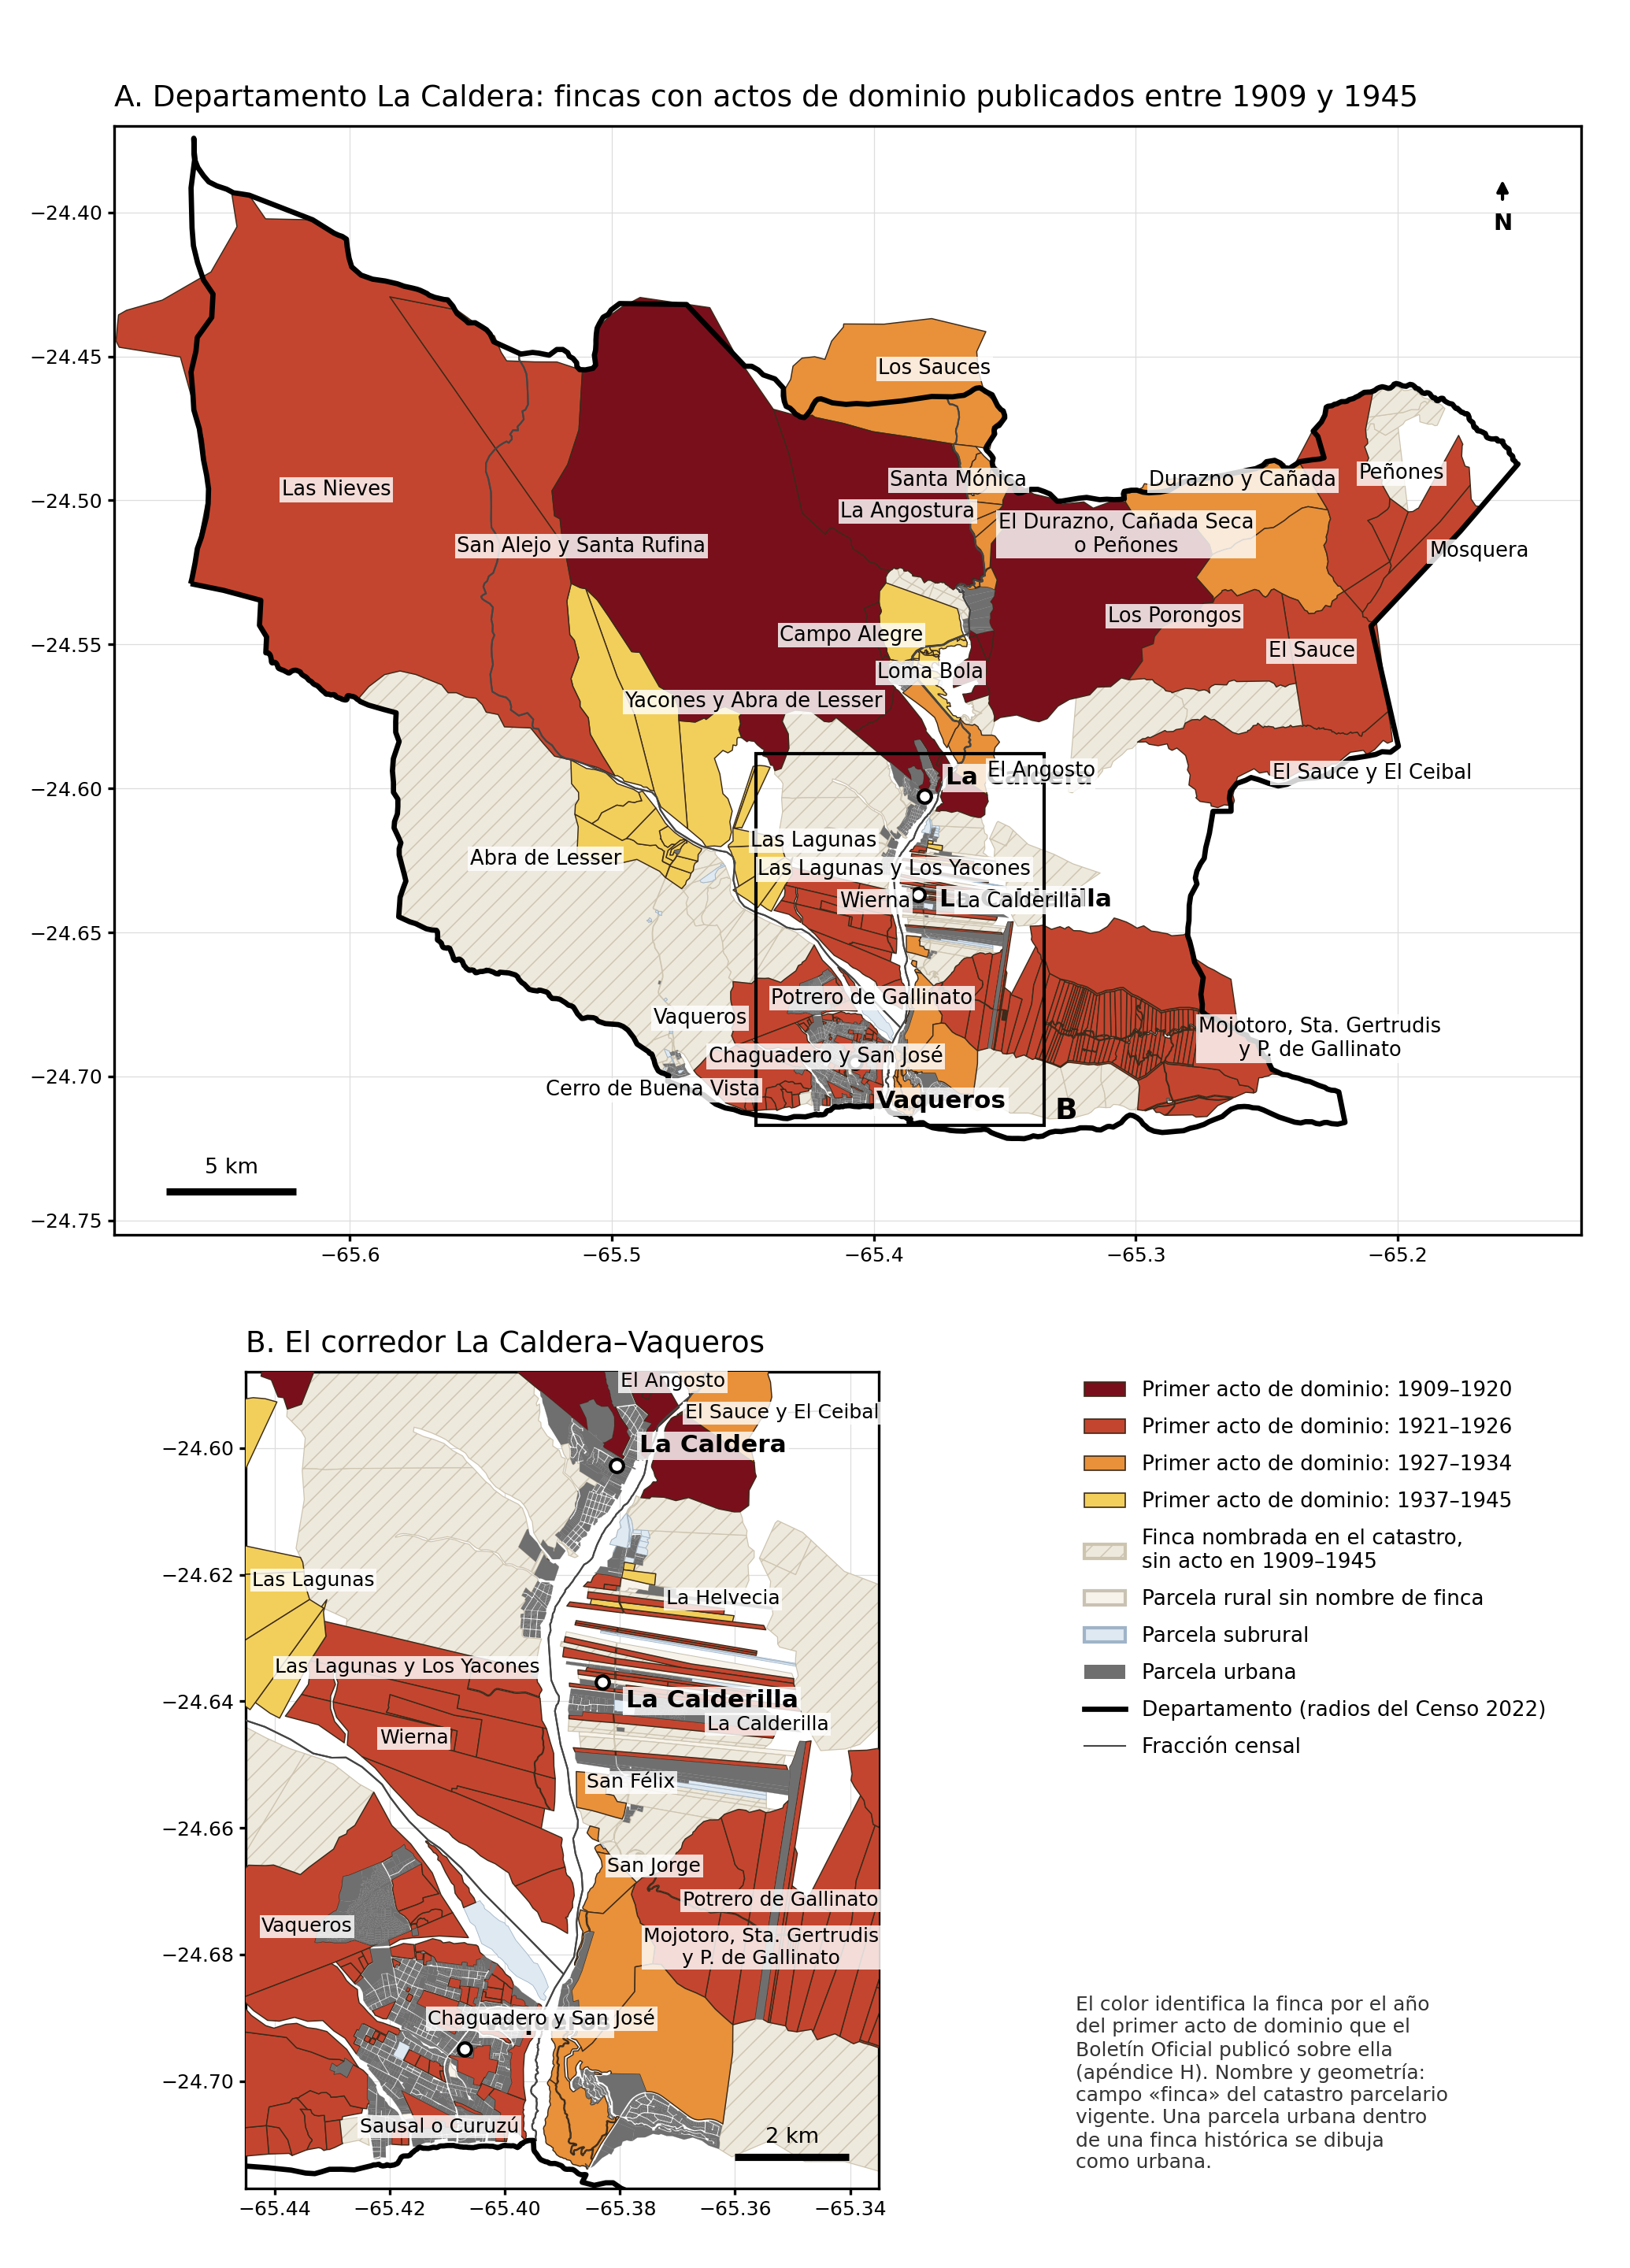
\includegraphics[width=\textwidth,height=0.84\textheight,keepaspectratio]{fig-fincas-historicas.png}
\caption[Las fincas del archivo en el catastro vigente]{\textbf{Las fincas del archivo en el catastro vigente.} A: parcelas del departamento cuyo campo «finca» del catastro parcelario coincide con una finca objeto de un acto de dominio publicado entre 1909 y 1945, coloreadas según el año del primer acto (apéndice \ref{cap:dominio}); en gris, las parcelas urbanas. B: el corredor La Caldera--Vaqueros. La coincidencia es de nombre, no de deslinde: el catastro no dice si los límites actuales son los de entonces. Elaboración propia con el catastro parcelario de la Provincia (IDESA, consultado en septiembre de 2026) y la cartografía de radios del Censo 2022 (INDEC). Elaboración propia; dibujo de \texttt{scripts/mapa\_fincas.py} del repositorio \texttt{mapas\_caldera} (apéndice \ref{cap:fuentes}).}\label{fig:fincas}
\end{figure}

\section{La finca Vaqueros, rematada en 1935}

El topónimo del municipio es el apellido de un propietario colonial. La finca que lo lleva
aparece en el archivo en 1935, y aparece en un remate.

\begin{ficha}{Aviso judicial --- B.O.\ Nº 1.582, 3 de mayo de 1935}
Por orden del Juez de Comercio, el martillero Antonio Forcada venderá el 27 de mayo la finca
\textbf{«Vaqueros o Entre Ríos»}, ubicada en La Caldera, «limitando: Norte, Anacleto Toranzo
y Teodolinda de Toranzo; Sud, Francisco López Cross y Mercedes Carrillo; \textbf{Este,
Francisco Urquiza\index{Urquiza, Francisco S.}}; Oeste, \textbf{camino nacional}».

Embargada en la ejecución hipotecaria \textbf{Banco Provincial de Salta contra Ramón
Bracheri}. Base: \$12.000. Seña: 20 por ciento.

\textit{Los apellidos se transcriben literales del escaneo; el del lindero norte admite
leerse Toranzo, Toranzos o Toranzoz, y conviene cotejarlo contra el original.}
\end{ficha}

Cuatro datos.

\textbf{La finca se llama «Vaqueros o Entre Ríos».} El segundo nombre la describe: está
entre ríos, que es exactamente la condición que ochenta años después hará que el río Vaqueros
sea el límite entre dos jurisdicciones y que ninguna administre el conjunto del cauce.

\textbf{Su lindero al este es Francisco Urquiza\index{Urquiza, Francisco S.}}, el mismo que en 1921 hizo deslindar Cerro
de Buena Vista, en 1924 obtuvo la concesión del río Wierna, en 1928 renunció a la Comisión
Municipal y en 1931 le ganó el juicio a la Provincia. En 1935 su propiedad limita con la
finca que da nombre al municipio.

\textbf{Su lindero al oeste es el camino nacional.} La finca da al camino real a Jujuy, hoy
Ruta Nacional 9: el mismo corredor que estructura el mercado de suelo del departamento
noventa años después.

\textbf{Y se remata por una ejecución hipotecaria del Banco Provincial.} Como las dos casas
quinta de 1927 y 1929 y como la estancia Potrero de Gallinato en 1922 y 1930, la tierra de
este departamento cambia de manos, en el registro público, principalmente por deuda. En todo el período relevado hasta esa fecha ---de 1908 a 1935--- este libro encontró un solo aviso de
venta voluntaria de finca, y también fue un remate: el que Alberto, Abel y Adolfo Murúa
pusieron en marcha por su cuenta en octubre de 1933 sobre La Despensa (apéndice
\ref{cap:dominio}). Todo lo demás son remates judiciales.

Es una observación sobre las fuentes antes que sobre el mercado. Las compraventas
particulares no se publican y los remates judiciales sí, de modo que el Boletín muestra
sólo la parte forzada de las transferencias. Pero esa parte forzada es la única que dejó
rastro público, y es sobre ella que se puede reconstruir algo.

\section{Cómo se describía un límite}

En marzo de 1910 se publicó el edicto de mensura de la finca Los Porongos, solicitada por
Francisco Alemán con poder de Mónica Diez de Costas. Sus límites eran, al poniente, «las
lomas altas que lindan con tierras de La Caldera y Sauces, hasta donde se hallan unos
mojones antiguos»; al norte, «la loma que viene dividiendo las tierras de Perico, que hoy
poseen los herederos de don Domingo Iriarte»; al naciente, «siguiendo dicha cuchilla al
encontrarse la loma conocida con el nombre de Las Víboras».

\textbf{Seis años después, la misma finca sale a remate y el aviso sí da la superficie.} En abril
de 1916 el martillero Enrique Sylvester anuncia la venta de «\textit{la mejor y más productiva finca
Los Porongos hoy San Luis}», por la ejecución de Enrique Werner contra \textbf{Humberto Graf von
Garnier Turawa}, con base de \$33.333,33 ---«\textit{o sean las dos terceras partes de su tasación
fiscal}»--- y remate fijado para el 15 de junio en el local del Jockey Bar. Declara
\textbf{5.359 hectáreas, 77 áreas y 83 centiáreas}, según el deslinde de los agrimensores Pfister y
Martin aprobado por el Departamento Topográfico, y repite los mismos límites de 1910 palabra por
palabra, agregando al sud «\textit{la cuchilla que sale del morro alto por el Poniente, conocida por
la del Tabacal o Pelada Muerta, que es la que divide estas tierras de las de la Despensa}» (B.O.\
Nº 600, h.\ 3).

\textbf{Con eso, Los Porongos es la segunda finca del departamento con algo parecido a una cadena.}
En 1910 la hace deslindar Mónica Díez de Costas; el edicto de deslinde de Loma Bola de febrero de
1916 la describe como «\textit{la que fue de Mónica Díaz de Cortes, hoy del conde Garnier de
Turava}»; en abril de 1916 se remata por ejecución contra ese mismo conde; y en 1932 el deslinde de
las cinco fincas de Silvano Ignacio Murúa\index{Murúa, Silvano Ignacio} la registra como «\textit{la
finca y la estancia Los Porongos, de don Daniel Linares}»\index{Linares, Daniel}. \textbf{Y el ejecutante no es un acreedor de paso.} En septiembre de 1912 el deslinde de esa misma
finca ---publicado entonces como «Los Porongos» o «San Luis»--- lo habían solicitado
\textbf{Pablo Enrique Wernner y Enrique Leconte}, y en 1913 un Pablo Enrique Wenner hace deslindar un
terreno propio en el departamento (apéndice \ref{cap:dominio}). Leconte era, ese mismo año, comisario
auxiliar del partido de Los Porongos.

\begin{cautela}
\textbf{Los tres avisos imprimen tres grafías ---Wernner, Wenner, Werner--- y este libro no las
unifica.} Lo que se afirma es lo que está impreso: quien en 1912 pidió el deslinde de esa finca lleva
el mismo apellido que quien en 1916 la ejecuta, con cuatro años de diferencia y sobre el mismo
inmueble. Que sean la misma persona es probable y no está acreditado, y se resuelve con el
expediente, no con el Boletín.
\end{cautela}

\textbf{Cuatro
eslabones, dos de ellos nuevos, y un solo dato de superficie en toda la serie.} Lo que falta ---quién
compró en la subasta de junio de 1916, si se realizó--- es exactamente lo que el expediente diría y
el Boletín no dice: ningún aviso de este departamento publica jamás el resultado de un remate.

Así se describía la propiedad rural del departamento en 1910: por lomas, cuchillas,
mojones antiguos y el nombre de quien poseía al lado. Sin coordenadas, sin superficie
declarada en el edicto, sin plano publicado. Ése es el material del que descienden las
matrículas que este libro persigue, y la razón de fondo por la cual establecer si una
proviene de otra exige un estudio de títulos y no una consulta.

\section{Una finca con cadena completa}

Hay un caso —uno solo— en el que este libro puede seguir un inmueble de punta a punta.

En enero de 1921 se ordena el deslinde de las fincas Cerro de Buena Vista y Sausal o Curuzú, en el partido de Vaqueros, de propiedad de Francisco S. Urquiza\index{Urquiza, Francisco S.}; en 1924 el mismo Urquiza obtiene concesión para regarlas con sobrantes del Wierna; y en 2014 la Secretaría de Ambiente convoca a audiencia por la Urbanización Cerro de Buena Vista sobre las matrículas 1713 y 1905. El capítulo \ref{cap:loteo} sigue esa secuencia.

Deslinde en 1921, agua en 1924, urbanización en 2014. Es la secuencia completa —título,
agua, loteo— documentada sobre un mismo inmueble a lo largo de noventa y tres años. Este
libro no afirma que las tres recaigan sobre idéntica superficie: un deslinde de hace un
siglo pudo subdividirse muchas veces. Afirma que el nombre y el lugar coinciden, que el
expediente de 1921 existe y está identificado, y que ése es el punto de partida natural
para reconstruir la cadena. Para los loteos del capítulo \ref{cap:loteo}, en cambio, ese punto de
partida todavía no aparece.

\section{Wierna: el recorrido completo de un nombre}

En octubre de 1908, el Boletín publica una sentencia sobre unos terrenos denominados «La
Finca». Se discute el título de don Bautista Wierna, y el fallo menciona «el callejón que
girando de Norte a Sud conduce al Molino de Wierna y después al Rosario de Lerma». La
demandada gana por prescripción treintañal, y el tribunal razona que «no figura en autos el
título de compra»: el reivindicante no pudo adquirir más derechos que los que tenía su
vendedor.

En 1921, Wierna ya no es un apellido sino un circuito electoral: figura entre los parajes
de una mesa receptora del departamento, junto a El Acheral, El Charcal, Las Garrapatas,
Los Porongos, Mesadas, Potrero de Valencia, Quesería, Santa Rufina y Yacones.

Hoy es un río, una finca con tres matrículas sobre las que se determinó la línea de ribera
en 2015, y el lugar de dos canteras de áridos concesionadas sobre tierra fiscal.

Apellido, paraje, curso de agua, unidad catastral, concesión minera. Ese recorrido es el
que siguen casi todos los topónimos de este departamento, y explica en una línea por qué
reconstruir su historia dominial exige leer un siglo de actos y no consultar un registro.

Vale la pena detenerse en cómo se resolvió aquel pleito de 1908. Se resolvió porque el
título no aparecía. La opacidad dominial del corredor no es un efecto del mercado
inmobiliario reciente: en el primer año del Boletín Oficial ya había un juicio que se
decidía por ausencia de instrumento traslativo de dominio, sobre la misma cuenca donde hoy
no puede establecerse si una matrícula proviene de otra.

\begin{cautela}
Hay que leer ese pleito con una reserva que la segunda lectura de 1908 hizo evidente. \textbf{La
sentencia no dice en qué departamento están los terrenos}, y el único rumbo que da es el de un
callejón que lleva al Molino de Wierna «y después al Rosario de Lerma», que queda al sudoeste de
la capital, mientras el río Wierna corre al norte. Puede tratarse de otra propiedad de un Wierna, fuera
de este departamento. Que el pleito sea «sobre la misma cuenca» es, entonces, una posibilidad y
no un dato; lo que se sostiene sin ella es que en 1908 un juicio de tierra se decidía por la
falta del título.
\end{cautela}

\section{El deslinde de 1932}

El documento más completo de este relevamiento entre los que nombran a la vez las fincas, sus
dueños y sus linderos es un edicto de deslinde de mayo de 1932, y conviene leerlo entero.

\begin{ficha}{Edicto de deslinde --- B.O.\ Nº 1.429, 27 de mayo de 1932}
Ángel R.\ Bascari, con poder y títulos de don \textbf{Silvano Y.\ Murúa} y de su esposa doña
Fanny Ovejero Lacroix de Murúa, solicita deslinde, mensura y amojonamiento de cinco fincas
del departamento La Caldera: \textbf{«Las Garrapatas», «Cañada Seca o Peñones», «El Durazno o
Peñones», «Los Matos» y «Severino»}.

Perito propuesto: Hermann Pfister\index{Pfister, Hermann}. Juzgado de 1ª Instancia y 1ª Nominación en lo Civil, Dr.\
Néstor Cornejo Isasmendi. Edictos por treinta días.

\textbf{Linderos nombrados en el edicto:} el puesto La Despensa, de los señores Adolfo,
Alberto y Abel Murúa; \textbf{la finca y la estancia Los Porongos, de don Daniel Linares\index{Linares, Daniel}};
el puesto Severino; la finca Peñones, de Silvano Y.\ Murúa; Peñones, de Francisco Sosaya ---«Sosauya», así en el edicto--- y
\textbf{herederos de Liborio Guerrero\index{Guerrero, Liborio}}; los herederos Campos; la sucesión de Silvano Murúa\index{Murúa, Silvano},
antes de Salvador Murúa; Ceibal o Algarrobal, de la sucesión del doctor José María Solá; El
Acheral, de los herederos Toledo; El Nogalito, de Salvador Rosa; y El Paraíso.

\textbf{Accidentes citados como límites:} el camino de la Punta de Agua, la Cañada de la
Iglesia, la mesada del Panteón, La Laguna, el Morro del Sunchal y la encrucijada del
Acheral.
\end{ficha}

\subsection*{El Durazno es una finca de 1932}

La tercera de las cinco se llama \textbf{«El Durazno o Peñones»}.

Es el nombre del loteo cuyos arroyos se determinaron en 2014, cuya agua para cuatrocientos
lotes se tramitó en 2015, cuyo plano se aprobó en 2021 y cuyas viviendas se inundaron en
2018 y 2019. En 1932 era una de las cinco fincas cuyo deslinde pidieron Silvano Y.\ Murúa y su esposa ante un juez civil ---un año después, el remate de La Despensa ya nombra como vecinos a la sucesión y a los herederos de Silvano Murúa, el padre homónimo, muerto antes de agosto de 1927 (apéndice \ref{cap:personas})---, con
límites al norte con los herederos Campos y al oeste con Daniel Linares\index{Linares, Daniel}.

Este libro no afirma que la finca de 1932 y la matrícula del loteo sean la misma superficie:
noventa años y varias particiones median entre una y otra, y establecerlo exige el estudio
de títulos que el apéndice \ref{cap:pedidos} reclama. Afirma que \textbf{el nombre existe como unidad de
dominio desde 1932 y que su deslinde judicial está identificado}, con juzgado, perito y
fecha. Es, para el loteo más discutido de este libro, el punto de partida de la cadena que
hasta aquí faltaba.

Y hay algo más en esa lista de cinco. \textbf{Las Garrapatas} figura como paraje del circuito
electoral de 1921. \textbf{Peñones} es el partido policial de 1909 —«Peñones y Chalchanio»,
con Liborio Guerrero\index{Guerrero, Liborio} como comisario auxiliar— y la finca cuyo título perdido se repuso
judicialmente en 1926. Las cinco fincas de un solo deslinde recorren, entre ellas, la mitad
de los nombres que este libro persigue.

\subsection*{Y dos años después se partió}

En septiembre de 1934, \textbf{Alberto Adolfo Murúa y Abel Murúa} solicitan el deslinde del
\textbf{Puesto Despensa}, «parte integrante de la estancia La Despensa», de aproximadamente
\textbf{dos mil seiscientas hectáreas}, con el mismo perito que dos años antes: Hermann
Pfister\index{Pfister, Hermann}.

Los límites que declara el edicto (Boletín Oficial Nº 1.549, 14 de septiembre de 1934) muestran lo que había pasado en el medio. Al norte, «propiedad de don Francisco Sosaya en parte y en otra con el
puesto Cañada Seca o Peñones \textbf{adjudicado al heredero Silvano Murúa\index{Murúa, Silvano Ignacio}}». Al sur, «el
puesto Los Matos, \textbf{adjudicado a la heredera Eulalia Murúa de Cornejo}». Al poniente,
«el puesto Las Garrapatas y Severino, de esta misma sucesión».

Son cuatro de las cinco fincas del deslinde de 1932 y el puesto de La Despensa ---que en 1932 figuraba como lindero, a nombre de Adolfo, Alberto y Abel Murúa---, ahora repartidos entre herederos con
nombre y apellido. \textbf{La partición hereditaria de un dominio grande es, en este
departamento, el mecanismo por el cual la tierra empieza a dividirse}, y aquí se lo ve
funcionar en tiempo real: en 1932 Silvano Y.\ Murúa y su esposa piden el deslinde del conjunto; en 1934 cada
puesto ya tiene adjudicatario entre los herederos de la sucesión de su padre, de la que él mismo es heredero (apéndice \ref{cap:personas}).

Es el mismo mecanismo que, sesenta años después, la literatura académica identifica como
origen del mercado de suelo de Vaqueros cuando se resuelve el juicio sucesorio de los
descendientes de Serrey\index{Serrey, Carlos}. No es una analogía: es el mismo procedimiento, en la misma
provincia, sobre el mismo tipo de dominio.

\subsection*{Y en 1936 se ejecutó}

Dos años después de repartida, la finca principal de la sucesión salió a remate por deuda de
los propios herederos.

\begin{ficha}{Remates judiciales de la finca La Despensa --- 1936}
El martillero Santiago Esquiú vende, por disposición del Juez de Comercio y en autos
seguidos por \textbf{Salvador Rosa contra Abel, Adolfo y Alberto Murúa}, la finca \textbf{La
Despensa}, en el partido del Sauce, departamento La Caldera.

\textbf{Límites:} «Norte, Francisco Sosaya y \textbf{Silvano Murúa\index{Murúa, Silvano Ignacio}}; Sud, \textbf{Eulalia
Murúa de Cornejo}; Este, José María Solá; Oeste, \textbf{Sucesión Murúa}».

Hubo \textbf{dos subastas}. La primera, el 6 de febrero de 1936, con base de \$23.333,32. La
segunda, semanas después, con base de \$25.000 --- \textit{un aumento poco habitual entre
una subasta y la siguiente, que conviene verificar contra el original antes de citarlo}.
\end{ficha}

La secuencia completa de esta sucesión cabe en cuatro años y muestra el mecanismo entero.

En \textbf{1932}, Silvano Y.\ Murúa y su esposa mandan deslindar cinco fincas, entre ellas
El Durazno o Peñones. En \textbf{1934}, los herederos Alberto Adolfo y Abel Murúa ---así, sin coma y dos veces, en el edicto; el deslinde de 1932, el remate de 1933 y la ejecución de 1936 nombran a tres personas: Adolfo, Alberto y Abel--- piden el deslinde del Puesto
Despensa y los límites ya declaran a cada puesto «adjudicado» a un heredero con nombre y
apellido. En \textbf{1936}, tres de esos herederos son ejecutados por un acreedor y la finca
mayor sale a remate, con los otros herederos como linderos.

Deslinde, partición, ejecución. \textbf{Es el ciclo completo por el cual un dominio grande se
fragmenta}, y en este caso se lo puede seguir entero en el Boletín Oficial porque las tres
etapas dejaron aviso público.

Ese ciclo importa por lo que viene después. La literatura académica identifica la resolución
de un juicio sucesorio como el origen del mercado de suelo de Vaqueros en los años noventa;
este libro documenta, sesenta años antes y sobre las fincas del otro municipio, el mismo
procedimiento funcionando de principio a fin. \textbf{La partición hereditaria no es un
antecedente del mercado de suelo caldereño: es su forma más antigua.}

\subsection*{Cuando una finca cambia de nombre}

En junio de 1937 se publica el deslinde de un inmueble llamado \textbf{«La Helvecia», antes
«Calderilla»}, en el departamento La Caldera. Es el documento más denso del período y lo es
por cuatro razones distintas.

\begin{ficha}{Deslinde, mensura y amojonamiento --- B.O.\ Nº 1.691, aviso Nº 3612}
Solicita \textbf{Hermann Pfister\index{Pfister, Hermann}}. Inmueble: \textbf{«La Helvecia», antes «Calderilla»}.

\textbf{Linderos:} «Norte, propiedad de \textbf{Augusto Regis\index{Regis, Augusto}}; Sud, propiedad de don
\textbf{Genaro Molina\index{Molina, Genaro}}; Naciente, herederos de don \textbf{Pedro Valencia}; Poniente, el
\textbf{Río de La Caldera}.»

Juzgado de 1ª Instancia y 1ª Nominación en lo Civil, Dr.\ Guillermo F.\ de los Ríos. Perito:
agrimensor Jorge de Bancarel. Auto del 10 de abril de 1937, conforme los artículos 570 y 474
del Código de Procedimientos. Publicación por treinta días en dos diarios y \textbf{por una
vez} en el Boletín Oficial.
\end{ficha}

\textbf{Primero: el topónimo se abandona y el nombre propio lo reemplaza.} «Calderilla» es un
paraje del departamento desde 1909 --- partido policial con comisario propio --- y sigue
nombrando hoy a una localidad y a un centro vecinal. La finca que lo llevaba pasa a llamarse
La Helvecia. En los mismos boletines, Vialidad financia los caminos «Calderilla al Desmonte
por Gallinato» y «Calderilla a Güemes por Gallinato»: \textbf{el nombre que la propiedad
abandona sigue nombrando la traza vial}. El topónimo sobrevive al dominio que lo usaba, que
es exactamente lo contrario del recorrido de Wierna.

\textbf{Segundo: el lindero al poniente es el río.} No un vecino: el curso. Una finca cuyo
límite occidental es el río La Caldera, deslindada judicialmente en 1937, en el mismo
departamento donde ochenta y cuatro años después una sentencia obligará a determinar qué se
construyó sobre las márgenes.

\textbf{Tercero: el lindero al norte preside el municipio.} \textbf{Augusto Regis\index{Regis, Augusto}} aparece
como propietario colindante ya en 1909 ---el remate de la décima parte del Angosto de Arrieta
lo nombra, con Julio Mercado y Susana Aguilera, como lindero al este--- y otra vez en junio de 1937, y veinte días después un decreto lo nombra
Presidente de la Comisión Municipal del Distrito de La Caldera. Es el mismo Regis\index{Regis, Augusto} que figura
como jurado suplente en 1908, que integró la comisión de defensas contra el río en 1910, que
fue designado miembro del cuerpo municipal en 1922, que lo presidía en 1933 y a quien
Vialidad encomendó en ese año la limpieza de un camino. \textbf{Treinta años de presencia
continua, y ahora también como titular de tierra lindera a la finca que se mensura.}

Y \textbf{Genaro Molina\index{Molina, Genaro}}, el lindero al sur, es el nombre del comisario auxiliar del partido
de La Calderilla en el decreto de 1909.

\textbf{Cuarto: el perito de 1932 es ahora el solicitante.} Hermann Pfister\index{Pfister, Hermann} había sido
designado perito en el deslinde de las cinco fincas de los Murúa en 1932 y en el del
Puesto Despensa en 1934. En 1937 pide el deslinde en nombre propio o por poder. En este mismo
corpus aparece además como inspector auxiliar de minas. \textbf{El técnico que mide el
departamento es, cinco años después, parte en una mensura.}

\begin{cautela}
Como siempre, coincidencias de nombre y no identificaciones registrales. Pero conviene
observar la acumulación: en un solo edicto de 1937, dos de los cuatro linderos llevan apellidos que el archivo registra en cargos públicos del departamento ---el presidente municipal y el comisario de un partido---, otro lindero es el río, y el solicitante es el perito oficial de las mensuras.

Este libro no extrae de ahí ninguna irregularidad. Extrae la constatación que la tercera
tesis enuncia: \textbf{durante la primera mitad del siglo, el conjunto de personas que
administraban el departamento y el conjunto de las que eran dueñas de su tierra se
superponían casi por completo.} Y una consecuencia práctica: quien quiera reconstruir el
dominio de este territorio hará bien en empezar por las nóminas de funcionarios.
\end{cautela}

\subsection*{Y una finca con folio, asiento y libro}

En febrero de 1937 se remata otra finca del departamento, y el edicto trae un dato que
ninguno de los anteriores traía.

\begin{ficha}{Remate judicial --- B.O.\ Nº 1.670, edicto Nº 3415}
Por orden del Juez de Comercio, en autos «Embargo Preventivo \textbf{Zulema Terán vs.\ Ramón
I.\ Juárez}», el martillero José María Decavi rematará con base de \$2.333,33 la finca
\textbf{«Chalchanio»}, departamento La Caldera, «con extensión y linderos le asignan sus
títulos registrados \textbf{Folio 342, asiento 438, Libro B La Caldera}».
\end{ficha}

Dos cosas.

\textbf{La finca está inscripta, y el edicto lo cita.} Folio, asiento y libro: la anotación
registral completa. Es la primera vez en las ediciones leídas que un aviso sobre el departamento remite al
registro en lugar de describir la propiedad por lomas y mojones. Ocho años después de la
catastración de 1929, el sistema registral funciona y los edictos lo usan.

Eso importa para el argumento del capítulo \ref{cap:opacidad}. Cuando este libro no puede establecer si una
matrícula proviene de otra, no está describiendo un territorio sin registrar: está
describiendo un registro que existe, funciona desde hace un siglo y no es consultable sin
arancel ni presencia física.

\textbf{Y «Chalchanio» es otro partido de 1909.} Figuraba entonces como «Peñones y
Chalchanio», con Liborio Guerrero\index{Guerrero, Liborio} como comisario auxiliar. Con éste, la lista de partidos de
1909 que reaparecen en el archivo como fincas con dueño, deuda o ejecución llega a seis:
San Alejo, Los Porongos, Potrero de Gallinato, La Despensa, \textbf{Vaqueros} ---rematada en
1935 como finca «Vaqueros o Entre Ríos» en la ejecución hipotecaria del Banco Provincial--- y
el partido de Peñones y Chalchanio, cuyos dos nombres reaparecen como fincas distintas.

\begin{cautela}
El ejecutado se llama \textbf{Ramón I.\ Juárez}, y en las mismas ediciones el comisario de
policía de La Caldera se llama \textbf{Ramón Juárez\index{Juárez, Ramón}}. El corpus no permite afirmar que sean
la misma persona ni descartarlo: la inicial del segundo nombre aparece sólo en el edicto.

Se consigna con esa reserva porque, de tratarse del mismo, sería otro caso de lo que este
libro viene documentando --- el comisario del departamento como propietario de una de sus
fincas --- y porque se resuelve leyendo el folio 342 del Libro B.
\end{cautela}

\textbf{Y ese folio vuelve a aparecer ocho años después, con otro ejecutado y con la finca ya
partida.}

\begin{ficha}{Remate judicial Nº 875 --- B.O.\ Nº 2.313 a 2.326, 21 de junio a 7 de julio de 1945}
Martillero \textbf{Leoncio M.\ Rivas}, por disposición del Juzgado de Paz Letrado Nº 1 de la
Capital, Dr.\ Marcelo Quevedo Cornejo, en autos «\textit{Embargo Preventivo Strachan, Yáñez y
Cía.\ vs.\ Martín Herrera}». Subasta del 30 de julio de 1945, base \textbf{\$671,01}, importe
del crédito en ejecución.

Bien: «\textit{\textbf{CUARTA PARTE INDIVISA DE LA FINCA ``CHALCHANIO''}, con extensión de 490
hs.\ 9 as.\ 36 ctms2.}», limitando al Naciente con el alambrado que la divide de la finca
«Mosquera»; al Norte, desde el esquinero en el \textbf{Abra del Angosto}, pasando por la
\textbf{loma de cal}, hasta un mojón en el \textbf{Abra de Chalchanio}; al Sud y parte del
Poniente, con un filo que la divide de la finca \textbf{«La Despensa»}; y al Oeste y Noroeste,
«\textit{con la fracción que le correspondió a don \textbf{Ernesto Echenique}}».

«\textit{Título registrado a Folio 342, Asiento 438 del Libro B, de Inmuebles de La Caldera. La
hipoteca ha sido registrada a Folio 108, Asiento 180 del Libro A, de Gravámenes de La Caldera.}»
\end{ficha}

Es el mismo folio, el mismo asiento y el mismo libro que cita el edicto de 1937. Entre una
fecha y la otra el ejecutado cambió ---Juárez en 1937, Herrera en 1945--- y el objeto de la
ejecución se redujo de la finca a \textbf{una cuarta parte indivisa} de ella, con al menos un
comunero nombrado, Ernesto Echenique, y con La Despensa como lindero sur.

\textbf{Es el mismo ciclo que este capítulo describe para La Despensa}, corrido ocho años y
una finca. Y refuerza la razón para pedir ese folio: no hay que leerlo para resolver una
homonimia, sino para reconstruir al menos dos traslaciones de dominio y una partición sobre un mismo asiento.

\begin{cautela}
El aviso no nombra paraje, no da número de catastro y no dice en ningún momento que la finca
esté «en La Caldera»: la ubicación descansa enteramente en el libro de registro. Los mojones
que menciona ---Abra del Angosto, loma de cal, Abra de Chalchanio--- y las fincas colindantes
«Mosquera» y «La Despensa» no fueron contrastados contra ninguna cartografía.

Una anomalía que queda registrada y no explicada: \textbf{el aviso declara vigencia hasta el 27
de julio y deja de publicarse el 7}. Las veinte ediciones siguientes, hasta el 13 de agosto, no
lo contienen, y ningún aviso posterior del mismo martillero corresponde a este juicio. El
corpus no dice si la subasta se suspendió, se levantó el embargo o el aviso se discontinuó por
otra razón.
\end{cautela}

\subsection*{Un padrón de parajes, en 1940}

Hay un documento que este relevamiento no buscaba y que ordena casi todos los topónimos de
este libro. No es un plano, no es un catastro y no es un registro: es un decreto electoral.

\begin{ficha}{Decreto del 30 de enero de 1940 --- ubicación de las mesas receptoras de votos y sus circuitos}
Dictado por el Ministerio de Gobierno, Justicia e Instrucción Pública conforme los artículos
29 a 31 de la Ley 122 de Elecciones de la Provincia, para el comicio del \textbf{3 de marzo de
1940}. Republicado en cuatro ediciones, siempre en anexo sin foliar.

La Caldera es el \textbf{Colegio Electoral Nº 2}, con dos circuitos y tres mesas:

\textbf{Circuito 5, Mesa 1} --- Escuela Elemental Mixta, La Caldera. Nueve parajes:
\textit{Calderilla, Chalchanio, Helvecia, \textbf{Getsemaní}, Peñones, Potrero de Castilla,
Pueblo, San Alejo, Severino}.

\textbf{Circuito 5, Mesa 2} --- Iglesia Parroquial, La Caldera. Treinta y un parajes:
\textit{Abra de la Sierra, Acheral, El Angosto, Angosto de Arrieta, Angostura, El Bordo,
Calderilla, Campo Alegre, Cañada Ancha, Corral de Barranca, Churcal, Los Chusos, Despensa,
Despensilla, Higueritas, \textbf{Potrero de Gallinato}, \textbf{Las Lagunas}, Los Matos,
Mesada, Monte de las Garrapatas, \textbf{Mosquera}, Nogalito, \textbf{Potrero de Valencia},
\textbf{Los Porongos}, Quesería, Santa Gertrudis, \textbf{Santa Rufina}, Los Sauces, La Sierra,
Wierna, Yacones}.

\textbf{Circuito 6, Mesa 1} --- Oficina del Registro Civil, Vaqueros. Siete parajes:
\textit{\textbf{Entre Ríos}, Estación F.C.C.N.A., Mojotoro, \textbf{Lesser}, El Túnel,
Vaqueros, \textbf{Villa Urquiza}\index{Urquiza, Francisco S.}}.
\end{ficha}

\textbf{Cuarenta y siete entradas y cuarenta y seis nombres distintos ---Calderilla figura en dos mesas---, y casi todos los que este libro persigue están ahí.} Getsemaní
---la matrícula 4366, a la que el edicto de agua de 2015 vincula con el loteo El Durazno, aprobado sobre la matrícula 6.558 (capítulo \ref{cap:ribera})--- figura como paraje
poblado y con mesa asignada en 1940. Las Lagunas es la finca cuya posesión treintañal se
tramitará cinco años después. Chalchanio es la finca que el remate de 1945 volverá a llevar
a subasta sobre el mismo folio, y Mosquera y Despensa son los dos linderos que ese remate
nombra. Potrero de Valencia es el lindero este del terreno cuya posesión treintañal promueve
Pfister\index{Pfister, Hermann} en 1945 ---«propiedad de la sucesión de Micaela de Valencia», según el edicto---, y
los herederos de Pedro Valencia eran ya, en 1937, el lindero naciente de La Helvecia. Potrero de Gallinato, Los Porongos, San Alejo,
Santa Rufina y Campo Alegre son partidos de 1909 ---el último, desde 1911---, fincas rematadas o fracciones expropiadas
en 1972. Y en el circuito de Vaqueros están Entre Ríos ---el otro nombre de la finca Vaqueros
rematada en 1935--- y una \textbf{Villa Urquiza}.

Lo que este decreto aporta no es un dato sino \textbf{una escala}: en 1940 el Estado sabía, y
publicaba, en qué parajes vivía la gente del departamento y a qué mesa le correspondía votar.
Es la lista más completa de unidades territoriales pobladas que este relevamiento encontró
entre el padrón de partidos de 1909 y la cartografía catastral de 2026, a treinta y un años del primero y a ochenta y seis
de la segunda.

\begin{cautela}
Un paraje electoral no es una finca ni una unidad catastral: nombra dónde vive gente que vota,
no dónde termina un dominio. Que «Getsemaní» sea paraje en 1940 no dice quién era su dueño ni
qué superficie tenía, y este libro no lo infiere. La correspondencia entre estos cuarenta y
seis nombres y las matrículas actuales es, exactamente, uno de los pedidos que el apéndice
\ref{cap:pedidos} dirige a la Dirección General de Inmuebles ---y ahora puede formularse con
una lista cerrada en lugar de con trece partidos.
\end{cautela}

\subsection*{Y el registro no reemplazó a los mojones}

El edicto de Chalchanio de 1937 es el primero de las ediciones leídas que identifica un inmueble por folio,
asiento y libro en lugar de describirlo por lomas y mojones. Sería cómodo leer eso como un
umbral: antes se describía, después se registraba.

\textbf{No es así, y hay un edicto de 1945 que lo desmiente.}

\begin{ficha}{Edicto Nº 460 --- posesión treintañal de la finca «Las Lagunas» --- 23 ediciones, enero a marzo de 1945}
Promovido por el procurador Diógenes R.\ Torres en representación de don \textbf{Gregorio
Maidana}, ante el Juzgado de Primera Instancia, Segunda Nominación en lo Civil, Dr.\ Roberto
San Millán. Auto del 30 de diciembre de 1944.

El inmueble se describe así, «\textit{según el título de adquisición de don Domingo Bejarano a
don Marcos Arroyo}»: «\textit{Desde el límite Norte, que divide la propiedad del otorgante
Arroyo con la del señor José Manuel Fernández hasta dar con un arroyo que baja de las cumbres
altas de Naciente a Poniente, denominado de ``Los Comederos'' o de ``El Barbecho'', y de
Naciente a Poniente, desde las cumbres altas de las serranías de La Caldera hasta dar con el
\textbf{Río de Los Yacones}, enfrentando con el arroyo de ``Las Carretas''}».

El auto ordena oficiar «\textit{al Sr.\ Juez de Paz de La Caldera}» para recibir la información
ofrecida, y preguntar a las oficinas «\textit{si el inmueble de referencia cuya posesión se
pretende acreditar, afecta o no propiedad fiscal o municipal}».
\end{ficha}

Ocho años después del edicto que citaba folio y asiento, una finca entera del departamento se
identifica ante la justicia \textbf{por vecinos y por cursos de agua}: sin superficie, sin
número de catastro, sin partida. Lo único cuantificado en el aviso es el importe de la
publicación, sesenta y cinco pesos.

De los cuatro nombres del título ---Maidana, Bejarano, Arroyo, Fernández--- la cadena de
adquisición sólo cubre a dos, y \textbf{Maidana no está en ella}: eso es exactamente lo que la
posesión treintañal viene a suplir. La misma vía que el Estado usó en 1943 para regularizar el
predio de la Comisaría, y que Hermann Pfister\index{Pfister, Hermann} usará seis meses después
en La Calderilla.

\textbf{Las dos formas de describir conviven}, y conviven con la tercera que el capítulo
\ref{cap:ribera} encuentra setenta años más tarde: pares de coordenadas Posgar que unas
resoluciones publican y otras remiten a la sede.

\subsection*{Los dueños eran los que gobernaban}

La lista de linderos merece leerse contra el capítulo \ref{cap:siglo}, porque los nombres coinciden de una
manera que no admite ser tratada como casualidad.

\textbf{Daniel Linares\index{Linares, Daniel}} figura como propietario de la finca y de la estancia Los Porongos.
Es el mismo Daniel Linares\index{Linares, Daniel} que en enero de 1910 integró la comisión de siete vecinos
designada para proyectar y ejecutar las defensas del pueblo contra las crecientes del río;
que la presidió; que en 1911 rindió las cuentas del déficit; y que en abril de 1922 fue
designado por el Interventor Nacional miembro de la Comisión Municipal de La Caldera.

\textbf{Silvano Ignacio Murúa\index{Murúa, Silvano Ignacio}}, que pide con su esposa el deslinde de las cinco fincas, no es el único
Silvano Murúa del expediente: el mismo edicto nombra como lindero a «la sucesión de Silvano
Murúa\index{Murúa, Silvano}»: su padre, nacido en 1855, muerto antes de agosto de 1927, del que el
titular es heredero. El que renunció a la Comisión Municipal en 1909 ---«Silvano J.\ Murúa» en el
decreto, reemplazado por Abelardo Figueroa--- y que integró la comisión de defensas de 1910 es el
hijo, entonces de veintiséis años: había nacido en 1882 y se había casado dos meses antes de la
renuncia (apéndice \ref{cap:personas}).

\textbf{Liborio Guerrero\index{Guerrero, Liborio}}, cuyos herederos aparecen como linderos, fue comisario auxiliar del
partido de Peñones y Chalchanio según el decreto de 1909.

\begin{cautela}
Corresponde el mismo cuidado de siempre. Se trata de coincidencias de nombre y apellido en
documentos separados por veinte y treinta años, no de identificaciones registrales; en un
departamento de pocos miles de habitantes los apellidos se repiten, y una sucesión
puede llevar el nombre del causante durante décadas.

Pero la coincidencia no es de un nombre: es de tres, y los tres ocupan en 1909, 1910 y 1922
los cargos que el capítulo \ref{cap:siglo} documenta —comisión municipal, comisaría de partido, comisión
de defensas del río—, y aparecen en 1932 como propietarios o causantes de las fincas
principales del departamento.

Lo que este documento permite afirmar, entonces, es lo que el capítulo \ref{cap:politica} sostiene por otra
vía cuando encuentra a un propietario de finca convertido en senador por el departamento:
\textbf{en este territorio, durante la primera mitad del siglo, quienes administraban el
municipio, vigilaban los partidos y proyectaban las obras contra el río eran los dueños de
la tierra sobre la que se hacían}. No es una imputación --- en 1932 no había otra forma de
gobernar un lugar así --- sino la descripción de una estructura, y es el antecedente más
antiguo de lo que la tercera tesis de este libro llama un dispositivo anterior al mercado.
\end{cautela}

\section{Un dato menor que confirma quiénes estaban}

Antes de llegar a la sucesión que abrió el mercado de suelo de Vaqueros, conviene registrar
una pieza lateral y elocuente. En 1934, la Sala en lo Penal de la Corte de Justicia resolvió
una causa por hurtos cometidos, según la carátula, \textbf{en las casas de Serrey\index{Serrey, Carlos} y de
Linares}, en el departamento de La Caldera.

No aporta nada sobre el dominio y este libro no lo usa para eso. Aporta otra cosa: que en
1934 las dos familias que este capítulo y el \ref{cap:siglo} vienen siguiendo --- la que casi sesenta años después abriría por partición hereditaria el mercado de parcelas de Vaqueros, y la del
presidente de la comisión de defensas del río de 1910 --- tenían casa en el departamento y
eran identificadas por su apellido en la carátula de un expediente penal.

\subsection*{La Curia y Serrey, linderos en el pueblo}

En noviembre de 1939 la \textbf{Curia Eclesiástica de Salta} promueve juicio de posesión
treintañal sobre un terreno del pueblo de La Caldera, ante el juez civil Carlos Cornejo
Costas. El edicto declara medidas irregulares --- ciento veintiséis metros al norte,
treinta y tres al sur, con un martillo de diez metros al sudeste --- y estos linderos:

«\textbf{Norte, Dr.\ Carlos Serrey\index{Serrey, Carlos}}; Sud, herederos Vidaurre y calle pública; Este, calle
pública; \textbf{Oeste, Dr.\ Carlos Serrey\index{Serrey, Carlos}}.»

Dos elementos de ese edicto conviene retener, porque los dos reaparecen ochenta años
después en municipios distintos del mismo departamento.

\textbf{La Iglesia adquiere por posesión treintañal.} No compra: acredita treinta años de
posesión pública y pacífica y pide que se le reconozca el dominio. Es el mismo instituto
que en 2015 usará la Provincia para regularizar el terreno de una escuela, y el mismo por el
cual en 1908 una demandada ganó un juicio de reivindicación porque el título del actor no
aparecía. En un territorio donde los títulos escasean, \textbf{la prescripción adquisitiva
no es un remedio excepcional sino una vía ordinaria de acceso al dominio.}

Y ochenta años más tarde, en Vaqueros, será también la Iglesia --- la Congregación de los
Hijos de la Inmaculada Concepción --- la que transfiera veintitrés hectáreas a un
fideicomiso para un desarrollo de doscientas veintisiete parcelas, según documenta el
capítulo \ref{cap:vaqueros}.

\textbf{Y el lindero, por dos costados, es Carlos Serrey\index{Serrey, Carlos}.} El mismo apellido cuya sucesión,
resuelta a principios de los años noventa, la literatura académica identifica como origen
del mercado de suelo de Vaqueros; el mismo que donó el terreno donde se levantó el edificio
municipal de ese municipio; y el mismo que llevaba Elena Serrey\index{Serrey, Elena} de González Bonorino, a
quien en 1986 se le expropió un inmueble de La Caldera para viviendas familiares ---su
parentesco con Carlos Serrey no consta (capítulo \ref{cap:expropiacion})---.

En 1939, Carlos Serrey\index{Serrey, Carlos} es dueño de los terrenos que rodean por dos lados a la Curia en el
casco del pueblo. \textbf{Los dos actores que en el presente aparecen convirtiendo suelo en
los dos municipios del departamento eran, hace ochenta y siete años, vecinos.}

\section{El padrón de 1944}

Hay un solo documento en todo este relevamiento que dice quiénes eran los propietarios del
departamento y cuánto valía lo de cada uno. Es de diciembre de 1944 y ocupa dos páginas del
Boletín Oficial.

El Jurado de Valuaciones publicó el \textbf{Revalúo General de la Provincia}, departamento por
departamento. El de La Caldera trae \textbf{cuarenta y siete partidas}, de la número 56 a la
184, con nombre y valuación. Los titulares son de todo tipo: personas, sucesiones
(«herederos de»), condominios («y otros») y una partida cuyos titulares eran menores de
edad, cuyos nombres este libro no reproduce por el criterio que fija el capítulo
\ref{cap:metodo}.
No hay decreto que lo introduzca ni subtotal que lo cierre: la
nómina entra directamente después de los avisos judiciales.

\textbf{Las trece mayores concentran el grueso del valor:}

\needspace{8\baselineskip}
{\sffamily\bfseries\footnotesize Revalúo General de la Provincia, departamento de La Caldera, diciembre de 1944\par}
\vspace{0.5em}
{\small
\setlength{\LTpre}{0.6em}\setlength{\LTpost}{1.2em}
\begin{longtable}{@{}p{1.4cm}p{7.4cm}p{3.0cm}@{}}
\toprule
\textbf{Partida} & \textbf{Titular} & \textbf{Valuación} \\
\midrule
\endhead
157 & \textbf{Urquiza\index{Urquiza, Francisco S.}, Francisco S.} & \$52.400 \\
104 & Rauchi, Celina Z.\ de & \$36.500 \\
80 & Sánchez, Juana Mercado de, y otros & \$26.400 \\
159 & Solá, Elvira Patrón Costa de & \$19.700 \\
82 & Bruzzo, José A.\ y Carlos M. & \$14.000 \\
170 & Ortiz, Elina Solá Patrón de & \$14.000 \\
152 & Yufra, Rosario & \$10.200 \\
96 & Ochoa, herederos de Concepción & \$8.900 \\
149 & Vivero, Sandalio & \$8.500 \\
169 & Berardi, Atilio & \$8.000 \\
88 & \textbf{Murúa, Silvano Ignacio} & \$7.600 \\
67 & Figueroa, Marcos B. & \$7.000 \\
105 & \textbf{Rejis} [\textit{sic}]\textbf{, Augusto} & \$6.400 \\
\midrule
\multicolumn{2}{@{}l}{\textit{Total de las 47 partidas publicadas}} & \textbf{\$353.100} \\
\bottomrule
\end{longtable}
}

Cinco cosas se leen ahí.

\textbf{Primera: Urquiza\index{Urquiza, Francisco S.} sigue siendo el mayor propietario de los que el revalúo publica.} Cincuenta y dos
mil cuatrocientos pesos, casi el quince por ciento de todo el valor publicado, y más del
cuarenta por ciento por encima del segundo. Veinte años después de la concesión del Wierna,
dieciséis después de su prisión preventiva y ocho después de perder el juicio de daños, su
posición patrimonial no se movió.

\textbf{Segunda: Murúa y Regis\index{Regis, Augusto} siguen ahí.} Silvano Ignacio Murúa, doce años después del
deslinde de las cinco fincas y ocho después del remate de La Despensa ---es la misma persona que el edicto de 1927 nombra \textbf{Silvano I.\ Murúa} y el de 1932, \textbf{Silvano Y.\ Murúa}: la inicial media cambia de un aviso a otro, pero el hombre es uno, el mismo que en 1924 y en 1932 pide deslindes junto con su esposa, María Fanny Ovejero de Murúa, y que en 1934 recibe como heredero el puesto Cañada Seca o Peñones---. Y «Rejis, Augusto»
--- así impreso --- que este libro identifica con el Augusto Regis\index{Regis, Augusto} que preside la comisión municipal y que el año anterior había dejado el cargo de comisario.

\textbf{Tercera: aparecen los apellidos de la elite provincial.} Elvira Patrón Costa de Solá y
Elina Solá Patrón de Ortiz suman treinta y tres mil setecientos pesos, casi el diez por
ciento del departamento. Son los apellidos que gobernaron Salta durante la década, y que
firman varios de los decretos que este libro transcribe.

\textbf{Y uno de esos apellidos ya era propietario veintisiete años antes.} Los dos deslindes de
la Calderilla publicados en 1917 los nombran: el del terreno de Juana Flores de Chaile linda al sud
con \textbf{Ildefonsa Burgos de Yugra} y al este con \textbf{la familia Yugra}, y el del Potrero
Gallinato, del mismo año, linda al oeste con \textbf{los herederos Yugra} (apéndice
\ref{cap:dominio}). No son titulares nombrados en un padrón fiscal: son linderos en un edicto
judicial, que es la forma más antigua en que este archivo registra una propiedad. \textbf{El revalúo
de 1944 no los encuentra: los vuelve a encontrar.}

\textbf{Cuarta: y aparecen los otros.} Mamani, Yugra, Apaza, Condori, Yavi, Yufra: apellidos de origen andino, con valuaciones que en su mayoría van de doscientos a cuatro mil pesos ---Rosario Yufra, con diez mil doscientos, es la excepción y figura entre las trece mayores---. \textbf{El padrón
registra las dos puntas del mismo territorio en la misma página.}

\begin{cautela}
\textbf{Y no aparecen en 1944: el archivo los tenía desde mucho antes, y con título.} El barrido
año por año del Boletín entre 1913 y 1932, que se hizo después de escribir este apartado, los
encuentra veintisiete años antes del revalúo y en las tres calidades que importan (capítulo
\ref{cap:siglo}):

\textbf{Como propietarios con deslinde judicial.} En 1917 se deslinda por el rumbo sud un terreno
en \textbf{La Calderilla} «\textit{de propiedad de doña \textbf{Juana Flores de Chaile}}», que
linda al sur con «\textit{terrenos de \textbf{Ildefonsa Burgos de Yugra}}», al este con
«\textit{propiedad de \textbf{familia Yugra}}» y al oeste con el río de la Calderilla (B.O.\ Nº
662). \textbf{Yugra es uno de los seis apellidos de este cuadro}, y en 1917 la familia tiene tierra
lindera con título suficiente para que un juez mande deslindar contra ella.

\textbf{Como causantes de sucesión ante el juez de paz del propio departamento.} El juicio
sucesorio de \textbf{don Delfín Chaile} se abre en octubre de 1918 por auto del Juez de Paz
propietario de La Caldera; los de \textbf{Simón Yufra} en 1924 y \textbf{Milagro Catacata} en 1927
se dictan y se firman en el pueblo.

\textbf{Y como autoridad.} El padrón de comisarios auxiliares de 1919 pone a \textbf{Delfín
Chaile} al frente de la Calderilla, a \textbf{Zacarías Maidana} en Potrero de Castilla y a
\textbf{Juan Cuchui} en Yacones; en 1929 el comisario de policía del departamento es
\textbf{Manuel Condori}, otro de los seis.

\textbf{Eso cambia lo que el cuadro de 1944 prueba.} No muestra la aparición de esas familias en
el padrón: muestra que en 1944 seguían ahí. \textbf{Y el descarte conviene decirlo también}: los
Apaza, Mamani y Aramayo que el barrido encuentra en 1919 y 1920 son de Guachipas, Carahuasi e
Iruya, y no de este departamento; el propio informe de barrido los identifica y los descarta.
Este libro no los cuenta.
\end{cautela}

\textbf{Y quinta: cuarenta y siete partidas para todo un departamento.} Si esas partidas fueran todas ---y la advertencia que sigue explica por qué no puede asegurarse---, un departamento de más de cien mil hectáreas estaría repartido entre menos de cincuenta titulares. Es la
estructura que el capítulo \ref{cap:tierra} encuentra setenta y cuatro años después en el Censo Agropecuario, cuando
una sola explotación concentra el cincuenta y uno por ciento de la superficie agropecuaria.
\textbf{La concentración no es un resultado del ciclo inmobiliario: es el punto de partida.}

\begin{cautela}
Dos advertencias sobre este cuadro.

La nómina publica \textbf{valuaciones fiscales, no superficies}. Un valor alto puede
corresponder a mucha tierra de poco valor o a poca de mucho, y el Boletín no distingue. Para
convertir estas cifras en hectáreas hace falta el padrón catastral, que el apéndice \ref{cap:pedidos} reclama.

Y las partidas no son correlativas: van de la 56 a la 184 con huecos. Eso puede significar que
la numeración es provincial y no departamental, o que se publicaron sólo las partidas
revaluadas. \textbf{Este libro no sabe cuál de las dos cosas es}, y por lo tanto no puede
afirmar que estos sean todos los propietarios del departamento en 1944.
\end{cautela}

\section{La sucesión Serrey}

La literatura académica sobre las transformaciones urbanas de Vaqueros sitúa la gran
expansión de loteos en la década del noventa e identifica, entre los factores de su origen,
uno de carácter estrictamente jurídico: la resolución de un largo juicio sucesorio de los
descendientes de Serrey\index{Serrey, Carlos}, que permitió regularizar a principios de esa década una parte
importante de los dominios y facilitó así la subdivisión y venta de nuevas parcelas.

Al mismo tiempo, el edificio de la Municipalidad de Vaqueros se levantó, bajo dirección de
Humberto Bini, en un terreno donado por la sucesión del doctor Carlos Serrey\index{Serrey, Carlos}. El municipio
había sido creado por ley provincial el 5 de agosto de 1970, y su primer intendente, Julio
Catalán Arellano, ejerció entre octubre de ese año y mayo de 1973.

\begin{cautela}
El mercado de suelo del municipio más dinámico del departamento no nace de una decisión de
política pública ni de una inversión externa: nace de un hecho de derecho sucesorio, la
partición de un dominio patricio históricamente indiviso. Antes de la sentencia, la tierra
existía como patrimonio familiar; después, como oferta.

Y el mismo linaje donó el terreno donde funciona el organismo que regula esa oferta. No
implica irregularidad alguna y no debe leerse como imputación. Implica que el municipio de
Vaqueros nace institucionalmente alojado en tierra donada por la familia cuya partición
hereditaria constituye el objeto principal de su función regulatoria posterior.

El apellido aparece además en los dos municipios y en posiciones opuestas. En 1986, la Ley
provincial 6354 declaró de utilidad pública y expropió un inmueble de Elena Serrey\index{Serrey, Elena} de
González Bonorino en la localidad de La Caldera —matrícula 1.303, 8.158,71 m²— con destino
a la construcción de viviendas familiares; su parentesco con Carlos Serrey\index{Serrey, Carlos} no consta. En Vaqueros, el linaje abre el mercado privado de parcelas por vía sucesoria y cede además, por dos expropiaciones de 1985 y 1986, tierra para viviendas y para la planta potabilizadora; en La Caldera, el mismo apellido cede tierra al Estado por expropiación para vivienda social (capítulo \ref{cap:expropiacion}).
\end{cautela}

\subsection*{Lo que este capítulo establece}

Las unidades territoriales que este libro persigue tienen más de un siglo. No son
fracciones creadas por el mercado inmobiliario: son las divisiones administrativas
históricas del departamento, que el fraccionamiento contemporáneo hereda, subdivide y
renombra.

El apéndice \ref{cap:dominio} ordena en una sola tabla las cincuenta y ocho operaciones de dominio que el archivo registra entre 1909 y 1945 ---remates, deslindes, particiones y posesiones treintañales---, con su bien, su causa, su martillero y su precio. Leída en vertical, muestra lo que este capítulo documenta caso por caso: que en 1932 y 1934 no había quien comprara tierra en este departamento al precio de tasación, y que la vía para regularizar un título era la misma para el Estado, para la Iglesia y para un particular.

Ésa es la tercera tesis del libro, y aquí queda establecida su base documental. Cuando el
capítulo \ref{cap:ribera} pregunte si una matrícula proviene de otra, estará preguntando por el último
eslabón de una cadena que arranca antes de que existiera el Boletín Oficial que la
publicaría.


\chapter{El departamento antes del mercado}

\label{cap:siglo}
El Boletín Oficial de Salta empieza a publicarse el 15 de octubre de 1908, y su archivo
descargable arranca con la edición número uno. Las dos primeras décadas de esa colección
contienen unas cuarenta menciones al departamento La Caldera. Son pocas, están dispersas y
ninguna es espectacular. Leídas juntas describen un territorio cuyas relaciones con el
Estado ya estaban planteadas en los términos en que siguen planteadas hoy.

\section{Un municipio que vendía su recaudación}

En febrero de 1909, el Boletín publica el cuadro completo de entradas y salidas del
municipio de La Caldera durante el ejercicio anterior. Es la primera rendición de cuentas
conocida del departamento y cabe en una página.

\begin{ficha}{Inversión de las rentas municipales, año 1908}
Elevado el 15 de enero de 1909 por \textbf{Ángel Fernández\index{Fernández, Ángel}}, Presidente Municipal, al
Ministro de Gobierno, que ordena publicarlo.

\textbf{Entradas:} saldo del año anterior \$283,77; \textbf{producido de la venta por
licitación de los impuestos municipales} \$1.150; derechos de cementerio \$50.
\textbf{Total: \$1.483,77.}

\textbf{Principales salidas:} al Consejo General de Educación, el 20\% adicional, \$200;
secretario y comisario municipal, \$180; farolero municipal, \$54; \textbf{limpieza del
camino nacional desde el Angosto de Arias hasta Castañares y parte de la Calderilla,
\$293,60}; alumbrado, talonarios y escritorio, \$91,90; \textbf{construcción de un lazareto
con motivo de la peste de la viruela, \$63,10}; festejos del 9 de julio, \$80,50; comisión
de señoras para la función del Rosario, \$65; media docena de sillas para la comisión
municipal, \$30.

Existencia en caja al cierre: \$280,12.

\textit{El cuadro cierra: entradas y salidas dan \$1.483,77. Pero la partida educativa no:
el 20\,\% de los \$1.200 que el propio cuadro declara son \$240, y el cuadro imprime \$200.}
\end{ficha}

La partida mayor de ingresos —\$1.150 sobre \$1.483, casi el ochenta por ciento— es «el
producido de la venta por licitación de los impuestos municipales». El municipio no
recaudaba: remataba el derecho a recaudar, y cobraba por adelantado un precio fijo. Quien
ganaba la licitación se quedaba con lo que lograra cobrar.

Ese arreglo tiene una consecuencia que atraviesa el siglo. Un municipio que vende su
recaudación no tiene incentivo ni capacidad para conocer su base imponible: no necesita
saber cuántos inmuebles hay ni cuánto valen, porque su ingreso no depende de eso.

Ciento siete años después, el capítulo \ref{cap:hacienda} documenta lotes urbanos con valuación fiscal de
tres cifras y un municipio cuya superficie crece sin que crezca su recaudación. No es la
misma institución, pero es el mismo problema, y aquí está su forma más antigua.

\textbf{Y hay algo más que este cuadro, leído contra los años que siguen, obliga a decir: no fue el
primero de una serie, fue el único.} Los siete años que van de 1910 a 1916 se leyeron edición por
edición, y cada uno de esos barridos registra el mismo cero: \textbf{el Boletín no publica en esos
siete años un solo balance municipal}, ni de este departamento ni de ningún otro municipio de la
provincia. Sumados, son siete años consecutivos sin una sola rendición de cuentas municipal publicada.

\begin{cautela}
El cero es del \textit{Boletín}, no de los municipios: que no se publicara no prueba que no se
rindiera. Lo que prueba es que \textbf{entre 1909 y 1922 la rendición municipal dejó de ser un acto
público}, y que la de 1908 ---elevada por el presidente municipal al Ministro de Gobierno, que ordena
publicarla--- es un caso aislado y no el primer eslabón de una costumbre. Cuando en 1922 el
departamento vuelva a aparecer con números, ya no será rindiendo cuentas: será un presupuesto que la
comisión municipal sanciona y el Poder Ejecutivo aprueba.
\end{cautela}

Dos datos más de ese cuadro. El gasto mayor del año —un quinto del presupuesto— fue
limpiar el camino nacional entre el Angosto de Arias, Castañares y parte de La Calderilla:
en 2014, la Dirección de Vialidad contrataría al mismo municipio para desmalezar banquinas
y construir badenes en ocho rutas provinciales. Y el único gasto sanitario del ejercicio
fue construir un lazareto durante la peste de viruela.

\section{El año institucional de 1909}

El mismo año en que se publica ese cuadro, el Boletín deja ver cómo se armaba el gobierno del
departamento. \textbf{El 13 de enero de 1909 el Poder Ejecutivo nombró por decreto a los cinco
miembros de la Comisión Municipal de La Caldera} (B.O.\ Nº 26, 1909, h.\ 4) ---Ángel Fernández\index{Fernández, Ángel},
Silvano Murúa (hijo)\index{Murúa, Silvano Ignacio}, el doctor Rafael Usandivaras, Jacinto
Guerrero\index{Guerrero, Jacinto} y Belisario Benítez--- y el decreto dice por qué lo hacía él:
los nombramientos no podían hacerse «\textit{conforme lo prescribe el art.\ 173 de la
constitución}» porque la mayor parte de esas corporaciones no había hecho el sorteo de
renovación por mitades. La excepción funcionaba como regla.

El artículo 2º completa el circuito. Las comisiones nombradas debían recibir de las cesantes el
archivo «\textit{y demás pertenencias}» y elevar al Poder Ejecutivo \textbf{las ternas para el
nombramiento de los jueces de paz} y \textbf{el presupuesto de gastos del año}. El municipio
proponía; la Provincia designaba y aprobaba. Es, con noventa y nueve años de anticipación, la
misma relación que el capítulo \ref{cap:hacienda} describe para el presupuesto municipal de
1932 y para el de hoy.

\textbf{Y después está lo que pasó con esos cinco.} Tres renunciaron en el año, y los tres
reemplazos salieron del mismo grupo de nombres: en febrero, Silvano Murúa\index{Murúa, Silvano Ignacio}
es reemplazado por \textbf{Abelardo Figueroa}\index{Figueroa, Abelardo} (B.O.\ Nº 36, 1909, h.\ 3); en abril, Jacinto
Guerrero\index{Guerrero, Jacinto} por \textbf{Adolfo Vidal} (Nº 51, h.\ 3); y en mayo ---el decreto no trae fecha impresa; se publica en la edición del 22 de ese mes--- el doctor Usandivaras por
\textbf{Augusto Regis}\index{Regis, Augusto} (Nº 58, h.\ 4). Los tres entrantes son los tres que en noviembre
de 1908 habían sido nombrados jurados de reclamos de patentes del departamento (capítulo
\ref{cap:fincas}). \textbf{La comisión municipal que termina 1909 está integrada, en tres de sus
cinco lugares, por el jurado de patentes de 1908.}

El caso de Jacinto Guerrero\index{Guerrero, Jacinto} muestra la escala del pueblo mejor que
cualquier descripción. En enero es miembro de la comisión municipal; en febrero, comisario
suplente de policía del departamento; en marzo, juez de paz suplente, en reemplazo de Augusto
Regis\index{Regis, Augusto}, que había renunciado a ese cargo (B.O.\ Nº 37, 1909, h.\ 3); en abril renuncia a la comisión
municipal. \textbf{El juez de paz propietario era Carlos Matienzo\index{Matienzo, Carlos}, que
firmaba también como secretario del cuadro de rentas municipales.} En un departamento de unos
doscientos inscriptos en el registro cívico ---el decreto de correlación de agosto de 1909
implica ciento setenta y siete inscriptos anteriores---, los cargos de juzgar, mandar la policía,
gobernar el municipio y clasificar el impuesto se repartían entre menos de diez personas.

\textbf{Y 1910 repite el esquema y lo aprieta.} En marzo, Abelardo Figueroa\index{Figueroa, Abelardo}
renuncia a la comisión municipal y entra en su lugar \textbf{Escolástico
Aparicio}\index{Aparicio, Escolástico M.} (B.O.\ Nº 146, 1910, h.\ 3); en abril, el mismo Aparicio es nombrado
\textbf{comisario de policía del departamento} (Nº 148, h.\ 3); en diciembre es \textbf{comisionado de
empadronamiento y clasificación de patentes} de Caldera (Nº 214, h.\ 3) y, en la última edición del año, vuelve a ser nombrado comisario y
figura entre los cinco miembros de la comisión municipal del año siguiente (Nº 219, h.\ 3). \textbf{Cuatro
cargos en un año, y dos de ellos a la vez}: el que mandaba la policía del departamento
integraba el cuerpo que gobernaba el municipio. El decreto de diciembre que designa esas
comisiones repite, palabra por palabra, el argumento de enero de 1909: no se puede aplicar el
artículo 173 de la Constitución. \textbf{Dos años seguidos de excepción es el régimen
ordinario.}

\textbf{Y 1912 lo cierra con la prueba del mecanismo.} El 28 de febrero, el decreto que renueva
los comisarios de todos los departamentos de campaña vuelve a nombrar para Caldera a
\textbf{Escolástico M.\ Aparicio}\index{Aparicio, Escolástico M.} (B.O.\ Nº 320, 1912, h.\ 3):
\textbf{es el quinto año seguido en que el mismo hombre clasifica el impuesto o manda la
policía del departamento}. En mayo, un decreto nombra los jueces de paz «\textit{de acuerdo con
las ternas presentadas por la Comisión Municipal}» (Nº 335, h.\ 3): el circuito que el decreto
de 1909 había ordenado ---el municipio propone, la Provincia designa--- está funcionando y deja
constancia escrita. Y tres semanas después, otro decreto integra esa comisión municipal, que
estaba «\textit{incompleta}» por la renuncia de Augusto Rejis\index{Regis, Augusto}
\textit{[sic]}, con \textbf{Daniel Linares}\index{Linares, Daniel} (Nº 338, h.\ 3), que ese mismo
año figura, en el aviso de remate de San Alejo, como propietario de la finca Angostura que linda
con ella por el este y por el sur.

Dos personas más completan el cuadro de ese año. \textbf{Jacinto Guerrero}\index{Guerrero, Jacinto} es, a la vez, comisario suplente del departamento y juez de paz suplente. Y
\textbf{Eustaquio Murúa}\index{Murúa, Eustaquio}, comisario auxiliar del partido de La Despensa
desde abril, es sorteado en septiembre como \textbf{titular de la segunda mesa receptora de votos}
del departamento, con Adolfo Vidal de primer suplente (Nº 362, h.\ 3). \textbf{El comisario del
partido presidía la mesa donde votaba el partido.}

\textbf{Y en 1913 el mismo hombre cambia de poder sin salir del departamento.} En febrero se
acepta su renuncia a la comisaría y lo reemplaza Julio del Solar (B.O.\ Nº 391, 1913, h.\ 3);
en abril, \textbf{el Poder Ejecutivo lo nombra juez de paz propietario} del departamento, «de
acuerdo con las ternas pasadas por la comisión municipal» (Nº 404, h.\ 3); en agosto y en
octubre firma, como juez de paz, los edictos sucesorios del pueblo; y en noviembre es
designado \textbf{comisionado para revisar las patentes de las casas de comercio} de Caldera
(Nº 448, h.\ 3). \textbf{Seis años seguidos: clasificador de patentes, comisario, juez de paz
y otra vez patentes.} \textbf{Y en mayo de 1914 vuelve al cuerpo municipal}: un decreto del 9
lo nombra miembro de la comisión municipal del departamento en la vacante que dejó
\textbf{Salvador Rosa}\index{Rosa, Salvador} al trasladar su domicilio a la capital (B.O.\
Nº 485, 1914, h.\ 1). \textbf{Son siete años seguidos, y el séptimo lo devuelve al punto de
partida.} La comisión municipal que lo propone para juez tiene ese año tres
miembros ---Daniel Linares\index{Linares, Daniel}, Camilo Cáceres y \textbf{Salvador
Rosa}\index{Rosa, Salvador}--- y el tercero es el mismo acreedor que en 1936 ejecutará a los
herederos Murúa y se quedará con el remate de La Despensa (capítulo \ref{cap:fincas}).

Y el jurado del registro cívico ---el que resuelve los reclamos sobre quién está inscripto para
votar--- lo integran en 1913 y otra vez en 1914 las mismas cuatro personas: Daniel
Linares\index{Linares, Daniel} y Augusto Regis\index{Regis, Augusto} como titulares, Adolfo
Vidal y Silvano Murúa\index{Murúa, Silvano Ignacio} como suplentes (Nº 385, h.\ 2, y Nº 448,
h.\ 3).

\textbf{Y el jurado de patentes de 1915, designado en noviembre de 1914, repite tres de esos
cuatro nombres y cambia uno.} Titulares, Daniel Linares\index{Linares, Daniel} y
\textbf{Bernardo Austerlitz}\index{Austerlitz, Bernardo}; suplentes, Adolfo Videl
\textit{[sic]} y Silvano Murúa\index{Murúa, Silvano Ignacio} (B.O.\ Nº 527, 1914, h.\ 2). Lo
firma el Presidente del Senado en ejercicio del Poder Ejecutivo. \textbf{Es la primera
aparición de Austerlitz en el departamento}, once años antes de figurar como propietario de San
Alejo y Santa Rufina en los pedimentos de 1925; que haya comprado la finca en alguno de los
remates de 1914 es hipótesis y no dato, porque ningún aviso publica el resultado de las
subastas.


\textbf{El resto de los cargos de 1914 confirma el esquema sin novedad.} En abril, el decreto
anual de comisarios de campaña nombra para Caldera a \textbf{Julio del Solar}, el mismo que
había reemplazado a Aparicio en febrero de 1913 (B.O.\ Nº 478, h.\ 1). En febrero se nombra
subcomisario de la \textbf{estación Mojotoro}, «\textit{jurisdicción del Departamento de la
Caldera}», a José Nogales, con antigüedad del 11 de octubre anterior; en julio, otro decreto
reorganiza esa misma subcomisaría y nombra a \textbf{Benjamín López}, dando las gracias al
cesante sin nombrarlo (Nº 469, h.\ 2, y Nº 504, h.\ 2 y 3). Y en noviembre se nombra comisario
auxiliar del \textbf{partido Los Porongos} a Carlos Bongarnier, «\textit{de acuerdo con la
propuesta elevada por el señor comisario de policía del departamento de Caldera}» (Nº 525,
h.\ 2), que es otra vez el circuito de 1909: el municipio o la policía del lugar proponen, la
Provincia designa.

\textbf{Una cosa más, que el archivo de estos años casi no da.} En septiembre de 1914 el
\textbf{juez de paz del departamento} ordena publicar el edicto del juicio sucesorio de don
Salustiano Caro, citando a herederos y acreedores, fechado «La Caldera, septiembre 3 de 1914»
(Nº 510, h.\ 4). El nombre del firmante no se alcanza a leer en la hoja y el año no da otro
acto que lo nombre. \textbf{Es el único acto de 1914 en que el departamento aparece como sede
de un juzgado de paz en funciones}, y el cargo lo ejercía, desde abril de 1913, el mismo
Aparicio.

\begin{cautela}
Los actos dicen los cargos, no las relaciones. Que los mismos apellidos ocupen los cuatro
escalones no prueba acuerdo ni familia: prueba que el conjunto de personas elegibles era chico.
Lo que sí puede afirmarse, porque está en los decretos, es que \textbf{la Provincia designaba,
el municipio proponía en terna y el mismo nombre podía ocupar dos cargos a la vez}.
\end{cautela}

\subsection*{Y 1915 repite el esquema, con una novedad y una retirada}

El año 1915 se leyó edición por edición al cierre de este trabajo: cuarenta y nueve ediciones,
de la 537 a la 586, con la 581 ausente del repositorio y sin ediciones de enero ni de la primera
semana de febrero (apéndice \ref{cap:fuentes}). Deja cinco actos del departamento, y \textbf{ninguno
de ellos es de tierra}.

\begin{ficha}{Los actos del departamento de la Caldera en 1915}
\textbf{26 de enero.} Decreto del Poder Ejecutivo: «\textit{Habiendo terminado el período que fueron
nombrados miembros de la comisión municipal, del departamento de la Caldera los señores Adolfo Vidal
y Angel Fernández}», nombra para ese cuerpo a \textbf{Eustaquio Murúa}\index{Murúa, Eustaquio} y otra
vez a \textbf{Adolfo Vidal}, «\textit{por el término de ley}». Firman Patrón Costas y Julio Cornejo
(B.O.\ Nº 540 del 17 de febrero, h.\ 2, folio impreso 2.077).

\textbf{13 de febrero.} Convocatoria a elecciones: Caldera figura \textbf{en las dos listas del mismo
artículo}, la de los departamentos que eligen representantes al Senado y la de los que eligen
diputados (Nº 539, h.\ 3).

\textbf{Mayo.} Decreto de supresión de puestos «por razones de renta»: entre veintitrés agentes de
comisarías de campaña, \textbf{uno de Caldera} (Nº 552, h.\ 2).

\textbf{2 de septiembre.} Edicto del \textbf{juez de paz del departamento}, \textbf{E.\ M.\
Aparicio}\index{Aparicio, Escolástico M.}, que declara abierto el juicio sucesorio de Asunción Espeche
González de Wayar y cita por treinta días a herederos y acreedores (Nº 568, h.\ 4, y Nº 569, h.\ 3).

\textbf{6 de diciembre.} Decreto que comisiona a una persona por departamento para la clasificación
general de patentes y el empadronamiento de los capitales en giro de 1916: por Caldera,
\textbf{Escolástico M.\ Aparicio}\index{Aparicio, Escolástico M.} (Nº 584, h.\ 2). Un decreto «de la
fecha» nombra los \textbf{jurados} que entenderán en los reclamos de ese empadronamiento: por Caldera,
\textbf{Daniel Linares}\index{Linares, Daniel} y \textbf{Silvano Murúa}\index{Murúa, Silvano Ignacio};
suplentes, \textbf{Adolfo Vidal} y Belisario Nieva (Nº 585, h.\ 2).
\end{ficha}

\textbf{La novedad es de personas, y es la misma forma de siempre.} El hombre que en septiembre firma
como juez de paz del departamento es, en diciembre, el que clasifica sus patentes: \textbf{octavo año
seguido con cargo} para Aparicio\index{Aparicio, Escolástico M.}, que el apéndice \ref{cap:personas}
sigue desde 1908. Y los jurados que van a resolver los reclamos contra esa clasificación son
\textbf{dos propietarios del departamento} ---Linares\index{Linares, Daniel}, dueño de Angostura y de
Los Porongos; Murúa\index{Murúa, Silvano Ignacio}, el que en 1932 hará deslindar cinco fincas
(capítulo \ref{cap:fincas})---, con un suplente, Adolfo Vidal, que once meses antes había sido
nombrado miembro de la comisión municipal por el mismo Poder Ejecutivo que ahora lo nombra jurado.

\begin{cautela}
Conviene decir qué prueba y qué no. \textbf{No prueba ningún acuerdo}, y el decreto que los nombra es
el mismo que nombra jurados en los otros veintidós departamentos. Prueba lo que el capítulo
\ref{cap:prospectiva} sostiene por otra vía: que en un departamento con poco más de quinientos
inscriptos, \textbf{quien clasifica, quien resuelve el reclamo contra esa clasificación y quien
administra el municipio salen de la misma lista, porque no hay otra}. La coincidencia no hizo falta
producirla.
\end{cautela}

\textbf{Y la retirada es de plata.} En mayo la Provincia suprime, por razones de renta, el agente de
la comisaría de campaña de Caldera, uno de los veintitrés que suprime en el mismo artículo. Cuatro
años antes había creado uno para Vaqueros por la obra del puente y por la explotación de canteras. En
las ediciones leídas hasta aquí \textbf{es la primera vez que el archivo registra la supresión de un
cargo del departamento y no su creación}, y ocurre en el año en que ese mismo departamento es
convocado a votar tres veces.

\subsection*{Y 1916 acumula los cargos en dos nombres}

El año 1916 se leyó también edición por edición, y es el tramo más limpio de los seis: las cuarenta
y nueve ediciones de la 587 a la 635, sin un solo salto, con sus 196 hojas (apéndice
\ref{cap:fuentes}). Deja doce actos del departamento, tres de ellos sobre la tierra ---el deslinde de
Loma Bola, el remate de Los Porongos y el segundo deslinde de Santa Mónica y Quitilipe, que el
apéndice \ref{cap:dominio} incorpora--- y nueve sobre los cargos. Los nueve caben en dos nombres.

\textbf{Escolástico Aparicio\index{Aparicio, Escolástico M.} renuncia y vuelve por la puerta de al
lado.} En febrero un decreto acepta su renuncia como miembro de la comisión municipal y nombra en su
lugar a Andrés Marín (B.O.\ Nº 593, h.\ 1). En abril, «\textit{de acuerdo con la terna elevada por la
Comisión municipal de la Caldera}», otro decreto lo nombra \textbf{Juez de Paz propietario} del
departamento «\textit{para el ejercicio del corriente año}» (Nº 601, h.\ 3). \textbf{La terna que lo
propone la eleva el cuerpo que acababa de dejar}, dos meses antes. Es el noveno año seguido con
cargo, y el mecanismo es el que el capítulo describe para 1912: los jueces de paz salen de ternas de
la comisión municipal, y la comisión municipal la designa el gobernador.

\textbf{Eustaquio Murúa\index{Murúa, Eustaquio} junta tres cargos en cinco meses.} El 4 de marzo lo
nombran \textbf{comisario de policía} del departamento, en la vacante que deja Manuel R.\ Cornejo
(Nº 596, h.\ 1). El 16 de marzo, \textbf{expendedor de guías}, «\textit{aceptase la fianza dada en su
favor por don Silvano I.\ Murúa}\index{Murúa, Silvano Ignacio}, \textit{por la suma de 500 pesos
moneda nacional}» (Nº 597, h.\ 2). Y el 5 de agosto, en un decreto que organiza el impuesto al consumo
departamento por departamento, \textbf{receptor del impuesto al consumo} por La Caldera (Nº 616,
h.\ 2). El mismo hombre que en enero de 1915 había sido nombrado miembro de la comisión municipal y
que en septiembre de ese año era candidato a elector de gobernador por el partido oficialista.

\begin{cautela}
\textbf{Tres cargos en un año no son un privilegio: son la aritmética de un departamento chico}, y es
la misma aritmética que produjo los cuatro cargos de Aparicio en 1910. Lo que sí merece registrarse es
\textbf{qué} cargos son. El comisario de policía, el expendedor de guías ---el que extiende el papel
sin el cual no se puede mover ganado--- y el receptor del impuesto al consumo son, los tres, el punto
donde el Estado toca la circulación de bienes del departamento. Y el fiador que responde por el
expendedor es un Murúa, de la familia que quince años después hará deslindar cinco fincas del
departamento (capítulo \ref{cap:fincas}).
\end{cautela}

\textbf{La comisión municipal cambia dos veces en el año} y las dos por renuncia: en febrero sale
Aparicio y entra Andrés Marín; en septiembre sale Adolfo Vidal ---que venía de 1915--- y entra
Salvador Rosa (Nº 624, h.\ 2). Ninguno de los dos decretos acompaña ni cita el escrito de renuncia que
dice haber aceptado, y tampoco se publica la terna que invoca el decreto del juez de paz:
\textbf{tres actos citados y no acompañados en un solo año}, sobre un cuerpo de cinco miembros.

\textbf{Y en diciembre, el departamento aparece por primera vez en la Cámara de Justicia.} La nómina
de juicios sentenciados en el tercer trimestre incluye «\textit{Juan Campilongo versus Amado Juárez,
venido en apelación del Juzgado de Paz «La Caldera», sección contrato}» (Nº 632, h.\ 2). Es la primera
constancia, en las ediciones leídas, de que una sentencia del juzgado de paz del departamento llegó a
segunda instancia.

\subsection*{Dos series que sólo se ven leyendo los nueve años juntos}

Los tramos de 1908 a 1916 se leyeron año por año, y cada barrido registró los cargos de su año. Puestos
en una sola columna, dan dos trayectorias que ninguno de ellos podía ver.

\textbf{La primera es la de Escolástico Aparicio}\index{Aparicio, Escolástico M.}, y el libro ya la
nombra año por año. Completa, es ésta:

{\footnotesize
\begin{longtable}{@{}p{1.1cm}p{11.4cm}@{}}
\toprule
\textbf{Año} & \textbf{Cargo, y acto que lo registra} \\
\midrule
\endhead
1908 & Clasificador de patentes generales de Caldera para 1909 (noviembre) y comisario de policía del departamento para 1909 (diciembre) \\
\addlinespace
1909 & Otra vez clasificador de patentes del departamento, para 1910 \\
\addlinespace
1910 & Miembro de la comisión municipal (marzo, por renuncia de Abelardo Figueroa\index{Figueroa, Abelardo}); comisario del departamento (abril); comisionado de empadronamiento y clasificación de patentes (diciembre) y, el mismo mes, otra vez comisario y otra vez miembro \\
\addlinespace
1911 & \textbf{Comisionado del empadronamiento de los capitales en giro y de la clasificación de patentes para 1912}, por decreto del Ministerio de Hacienda del 9 de noviembre (B.O.\ Nº 295, h.\ 2) \\
\addlinespace
1912 & Comisario de policía del departamento (28 de febrero) \\
\addlinespace
1913 & Renuncia a la comisaría en febrero; \textbf{juez de paz propietario} por terna de la comisión municipal el 18 de abril; firma como tal el sucesorio de Gabriel Ruiloba en octubre; comisionado para revisar las patentes de las casas de comercio en noviembre \\
\addlinespace
1914 & Miembro de la comisión municipal, en la vacante de Salvador Rosa\index{Rosa, Salvador} (9 de mayo) \\
\addlinespace
1915 & Juez de paz del departamento (firma el edicto sucesorio en septiembre); comisionado de la clasificación de patentes de 1916 (6 de diciembre) \\
\addlinespace
1916 & Renuncia a la comisión municipal en febrero; juez de paz propietario en abril, por terna de esa misma comisión \\
\bottomrule
\end{longtable}
}

\textbf{Nueve años seguidos con cargo, bajo tres gobernadores.} Pero lo que la serie completa agrega no
es el número: es \textbf{cuál} es el cargo. En seis de los nueve años ---1908, 1909, 1910, 1911, 1913 y
1915--- lo que ocupa es el puesto que \textbf{clasifica o empadrona a los contribuyentes del
departamento}. La comisaría y el juzgado de paz son la excepción. Este libro lo venía presentando como
el hombre de los cuatro cargos de 1910; el archivo dice que es, antes que nada y durante casi una
década, el que fija cuánto paga cada comercio de La Caldera.

\textbf{La segunda es la de Eustaquio Murúa}\index{Murúa, Eustaquio}, y va en sentido contrario: de un
partido al departamento entero. En 1912 y 1913 es comisario auxiliar del \textbf{partido de La
Despensa}, uno de los trece. En enero de 1915 lo nombran \textbf{miembro de la comisión municipal} y en
septiembre es candidato a elector de gobernador por el partido oficialista. Y en 1916 junta, en cinco
meses, la comisaría de policía del departamento, la expendeduría de guías y la receptoría del impuesto
al consumo. \textbf{Cuatro años para pasar de auxiliar de un partido a los tres cargos que tocan la
circulación de bienes de todo el departamento.}

\textbf{Y los partidos tienen su propia rotación.} Los decretos anuales de comisarios auxiliares
permiten armar, por primera vez, quién mandaba dónde y por cuánto tiempo:

{\footnotesize
\begin{longtable}{@{}p{1.9cm}p{1.95cm}p{1.95cm}p{1.95cm}p{1.95cm}p{1.8cm}@{}}
\toprule
\textbf{Partido} & \textbf{1909} & \textbf{1911} & \textbf{1912} & \textbf{1913} & \textbf{1914} \\
\midrule
\endhead
Calderilla & Genaro Molina & Genaro Molina & Genaro Molina & Genaro Molina & --- \\
\addlinespace
Los Porongos & Teodoro Reyes & Teodoro Reyes & --- & Enrique Leconte & Carlos Bongarnier \\
\addlinespace
La Despensa & Francisco Leeds & Guillermo Wotton & Eustaquio Murúa\index{Murúa, Eustaquio} & Eustaquio Murúa\index{Murúa, Eustaquio} & --- \\
\addlinespace
Vaqueros & Adolfo Agote & --- & Jesús Ramírez & Guillermo Villanueva & --- \\
\addlinespace
San Alejo & --- & Ángel Fernández\index{Fernández, Ángel} & Ángel Fernández\index{Fernández, Ángel} & Manuel Ramos & --- \\
\addlinespace
Los Peñones & Liborio Guerrero & --- & Teodoro Reyes & --- & --- \\
\bottomrule
\end{longtable}
}

Dos cosas saltan. \textbf{Calderilla no rota}: el mismo hombre cuatro años seguidos, y es el único
partido así. Y \textbf{Teodoro Reyes no desaparece de Los Porongos: se muda a Los Peñones}, el mismo
hombre que en 1909 había sido además veedor del Código Rural por Los Porongos. Los cuadros están
armados con los decretos que cada barrido fichó; los guiones no dicen que el partido no tuviera
comisario, sino que el decreto de ese año no lo nombra o no fue fichado.

\subsection*{Y 1917 pone al aserrador en la comisión municipal}

El año 1917 se leyó también edición por edición, y es el más flojo de los once años que este libro leyó enteros: faltan la
edición 640 entera y cuarenta de las 329 hojas, y el entorno no permitió OCR propio, de modo que
doscientas trece hojas se leyeron sólo por la capa de texto del PDF, a unos 150 ppi (apéndice
\ref{cap:fuentes}). Con esa reserva, deja nueve actos del departamento, tres de ellos deslindes que el
apéndice \ref{cap:dominio} incorpora.

\textbf{La comisión municipal se renueva entera el 4 de enero} ---decreto 1056: Daniel
Linares\index{Linares, Daniel}, Andrés Marini y Camilo Cáceres, «\textit{por un nuevo período}»--- y
diecinueve días después, el decreto 1085 nombra jueces de paz del departamento «\textit{de acuerdo con
las ternas elevadas por la H.\ Comisión Municipal}»: propietario, \textbf{Escolástico M.\
Aparicio}\index{Aparicio, Escolástico M.}; suplente, Casimiro Cáceres. \textbf{Décimo año seguido con
cargo}, y la terna la eleva un cuerpo que tenía diecinueve días de renovado. En febrero, el decreto
1101 vuelve a poner a \textbf{Eustaquio Murúa}\index{Murúa, Eustaquio} de comisario de policía del
departamento, el mismo cargo que tenía desde marzo de 1916.

\textbf{Y uno de los tres renovados usa el mes siguiente.} El \textbf{Camilo Cáceres} que el decreto 1056 confirma en la comisión municipal el 4 de enero es el mismo \textbf{Camilo Cácere} ---así, sin la ese final, en el impreso--- que \textbf{quince días después} se presenta «\textit{con títulos bastantes}» a pedir el deslinde, la mensura y la división de condominio de la finca Potrero Gallinato, y obtiene el auto del juez de feria el 19 de enero. \textbf{Quince días entre el nombramiento en el cuerpo que administra el departamento y el escrito que pone en movimiento la justicia sobre una de sus fincas.} Las dos cosas son enteramente legales y no se sigue de ellas ninguna irregularidad: se sigue, otra vez, que en este departamento el que administra y el que pide son la misma lista de apellidos.

\textbf{Y en septiembre entra a ese cuerpo el hombre del aserradero.} El decreto 1377 nombra miembro
de la comisión municipal, en reemplazo de Andrés Marini que renunció, a \textbf{Rafael
Delgado}\index{Delgado, Rafael}. Diecinueve años después, un Rafael Delgado será el dueño del
aserradero del pueblo cuya maquinaria se remata sin base a instancia de una casa comercial de la
capital, y en el mismo año figurará en el nombramiento de jueces de paz del distrito (capítulo
\ref{cap:tierra}). \textbf{Si es la misma persona ---coincidencia de nombre, como siempre, y no
identificación registral---, la única industria documentada del pueblo estuvo sentada en su comisión
municipal desde 1917.}

\textbf{El cuarto nombre del año es el mismo de los tres anteriores.} Daniel
Linares\index{Linares, Daniel}, renovado en la comisión municipal el 4 de enero, es en febrero
\textbf{candidato a Diputado por Caldera} por el partido «Unión Provincial», en la nómina que publica
la Junta de Escrutinio para la elección del 4 de marzo. Y el departamento elige ese año \textbf{un
diputado y ningún senador}, contra el senador y el diputado que le correspondían en 1915: el decreto
de convocatoria lo pone en la lista corta.

\textbf{Y el mismo año, el mismo apellido tiene tierra del otro lado del límite.} Un edicto de deslinde de Campo Santo nombra a \textbf{Daniel Linares}\index{Linares, Daniel} como lindero este de la finca Ántila (B.O.\ Nº 672, h.\ 6), y otro, de la finca «\textit{San Pablo o Puesto Viejo}» del mismo departamento, pone a \textbf{Luis Linares}\index{Linares, Luis} de lindero sud, con el río Mojotoro al oeste (Nº 662, h.\ 3). El miembro de la comisión municipal de La Caldera y candidato a diputado por el departamento era, a la vez, propietario colindante en el departamento vecino.

\begin{cautela}
\textbf{Cuatro actos citados y no acompañados en un año de nueve actos.} Dos son renuncias que el Boletín da por hechas sin publicarlas: la de Andrés Marini a la comisión municipal y la de Emilio Fressart al puesto de subcomisario \textit{ad honorem} del partido de Mojotoro, que el decreto 1419 dice haber aceptado «en la fecha». El tercero son \textbf{las ternas} que el decreto 1085 invoca para nombrar a los jueces de paz y que no se publican. Y el cuarto, los \textbf{títulos y el dictamen del Agente Fiscal} en que se funda el auto de deslinde del Potrero Gallinato. Es el mismo mecanismo que el capítulo documenta para 1916: el cuerpo se rehace, y la justicia se mueve, por escritos que nunca se leen.

\textbf{Y una precisión sobre el perito}, porque el dato podría leerse de más: Herman Pfister\index{Pfister, Hermann} firma los tres deslindes del departamento, pero también es el perito propuesto en otros tres del mismo año que no son de aquí. \textbf{No es el agrimensor de La Caldera: es el agrimensor de la zona}, y que aparezca en todo lo que se mide dice más del tamaño del oficio que de ningún vínculo con el departamento.
\end{cautela}

\subsection*{Y en 1918 el departamento fue municipio electivo durante siete semanas}

El año 1918 se leyó también edición por edición y es el octavo tramo: las ediciones 684 a 736,
534 hojas, sin la 703, sin OCR propio y con un techo de 150 ppi (apéndice \ref{cap:fuentes}).
Dejó \textbf{veintisiete actos del departamento}, ninguno de dominio ---la ficha número
veintiocho del barrido es un falso positivo que este capítulo consigna más abajo. Y dejó, sobre todo, \textbf{el
episodio institucional más importante que este libro encontró antes de 1983}.

\begin{ficha}{Decreto N.\ 1.557 en acuerdo de Ministros --- Salta, 4 de marzo de 1918}
Considerando «\textit{que por la renta recaudada el año próximo pasado, está suficientemente
constatado}» que catorce departamentos y distritos ---\textbf{Rosario de la Frontera, Rosario de
Lerma, Cerrillos, Campo Santo, Metán, La Candelaria, Caldera, Chicoana, Orán, La Viña, Güemes,
Galpón, La Merced y Embarcación}--- «\textit{poseen una renta superior al mínimun de \$ 5.000
establecido}», el Gobernador dispone que desde el \textbf{1.\ de julio} dejen de ser Comisiones
Municipales y pasen a ser \textbf{Municipalidades electivas}.

El artículo 6 pone la inscripción, los actos preparatorios y la elección misma a cargo de las
propias Comisiones Municipales salientes. El artículo 7 manda sortear a los miembros para la
renovación del artículo 173 de la Constitución. Firman Cornejo y Zuviría.
\textit{(B.O.\ Nº 693, 8 de marzo de 1918, h.\ 1 a 3.)}
\end{ficha}

\textbf{Siete semanas después se deshizo, y se deshizo sólo para La Caldera.}

\begin{ficha}{Decreto N.\ 1.660 en acuerdo de Ministros --- Salta, 24 de abril de 1918}
«\textit{Habiéndose incluido entre las Comisiones Municipales, convertidas en Municipalidades
por decreto N 1.557, la del Departamento de la Caldera, cuya renta no alcanza a la suma de \$
5.000, pues en su Cálculo de recursos correspondiente al año próximo pasado, que haciendo a la
suma de \$ 6.471.44, se encuentra agregada la suma de \$ 3.083.94, como saldo del año anterior,
lo que ha motivado un error de apreciación en los datos que han servido de base para dictar el
decreto aludido, siendo en realidad la renta anual de dicha Comisión Municipal de \$ 3.387.50}».

Y considerando «\textit{que por los fundamentos del decreto ya citado y las disposiciones legales
pertinentes, el departamento de la Caldera \textbf{no está en condiciones de ser administrado por
una Municipalidad electiva}}», el artículo 1 deja sin efecto el decreto 1.557 en cuanto la
convierte.

La fecha se imprime «\textit{Salta, Abril 24 de 1913}» [\textit{sic}]: el último dígito se leyó a
600 ppi y la única lectura posible es 1918, porque la edición que lo publica es del 3 de mayo de
1918. Firman Cornejo, Zuviría y Alvarado.
\textit{(B.O.\ Nº 701, 3 de mayo de 1918, h.\ 2, pág.\ 148.)}
\end{ficha}

\begin{cautela}
\textbf{La cuenta cierra y por eso importa.} \$ 6.471,44 menos \$ 3.083,94 da exactamente \$
3.387,50, que es la renta que el decreto declara real. No hay error aritmético: lo que hubo fue
un saldo del ejercicio anterior computado como recurso del año, y esa sola línea contable es la
que decide si un departamento se gobierna a sí mismo o lo gobierna un cuerpo designado.

\textbf{El departamento quedó a mil seiscientos doce pesos con cincuenta centavos de tener
municipalidad electiva.} Es más que todo el presupuesto municipal del departamento diez años
antes, que en 1908 era de mil cuatrocientos ochenta y tres pesos (capítulo \ref{cap:opacidad}).

\textbf{Y la decisión no la tomó nadie contra el departamento.} La tomó una lectura de su propio
cálculo de recursos, hecha en la capital, sobre una planilla que el departamento había elevado.
Es la forma más temprana del mecanismo que el capítulo \ref{cap:opacidad} describe cien años
después: el criterio se aplica sobre un número que el interesado no controla y que nadie está
obligado a explicarle.
\end{cautela}

\textbf{Y un mes después se deshizo para todos.} El \textbf{decreto N.\ 50 del 21 de mayo de
1918}, ya del Interventor Nacional, deja sin efecto el 1.557 \textbf{entero} ---no sólo para La
Caldera--- y suspende la inscripción de electores abierta en los Registros; las Municipalidades y
comisiones existentes continúan hasta que se provean los medios de reemplazarlas
\textit{(B.O.\ Nº 704, h.\ 7 y 8)}. De los catorce departamentos que iban a elegir su gobierno
comunal en julio de 1918, ninguno lo eligió.

\begin{cautela}
Conviene medir qué prueba y qué no.

\textbf{Lo que prueba:} que en 1918 el criterio para tener gobierno municipal propio era un piso
de renta, que La Caldera lo superaba en el papel y no en el cálculo depurado, y que el propio
Estado provincial rehízo la cuenta y la revirtió en siete semanas.

\textbf{Lo que no prueba:} que el departamento hubiera conservado la municipalidad si el decreto
50 no hubiera existido, porque ése la quitó a los catorce. La secuencia de La Caldera es anterior
y es específica: fue el único de los catorce al que se le revisó la renta uno por uno.

\textbf{Y lo que deja establecido para el resto del libro:} que la condición de \textbf{tercera
categoría} con que el departamento aparece en 1983, y que la clasificación estadística M3
todavía arrastra en 2022 (capítulos \ref{cap:poblacion} y \ref{cap:politica}), no empieza con la
Ley 1349 de 1933. En 1918 ya se decidía por renta, y el departamento ya no llegaba.
\end{cautela}

\subsection*{Trece partidos, otra vez, y los mismos apellidos}

El \textbf{decreto 1.564 del 7 de marzo de 1918} nombra los comisarios auxiliares del
departamento «\textit{de acuerdo con las propuestas elevadas por el Comisario del Departamento de
la Caldera}», y al hacerlo enumera en una sola lista \textbf{el Comisario Suplente del Pueblo y
los comisarios auxiliares de trece partidos}: Pueblo, Mojotoro, La
Calderilla, Vaqueros, Potrero de Gallinato, Lesser, \textbf{Yacones}, Potrero de Castillo, Potrero
de Valencia, La Despensa, «\textit{Peñones y Chalchami}» [\textit{sic}], Los Porongos, «\textit{Los
Sauces y Campo Alegre}» y «\textit{San Alejo y Santa Rufina}».

\textbf{Es la misma división que el capítulo \ref{cap:fincas} lee en 1909, nueve años después y
con los mismos nombres.} Y tres de los nombrados vienen de esa lista: \textbf{Liborio
Guerrero}\index{Guerrero, Liborio}, comisario auxiliar de Peñones y Chalchanio en 1909, vuelve al
mismo par de partidos en 1918; \textbf{Zacarías Maidana} y \textbf{Genaro Molina} también son
nombres de 1909. Un cuarto viene del año anterior: \textbf{José Nogales}, que en 1917 figura como
lindero este del Potrero Gallinato en el deslinde de esa finca (apéndice \ref{cap:dominio}), es
en 1918 el comisario auxiliar de ese mismo partido ---y renuncia el 20 de junio, a los tres meses
y medio (decreto 165, B.O.\ Nº 709, h.\ 6).

\begin{cautela}
\textbf{El topónimo Yacones aparece impreso en este decreto y ninguna búsqueda lo devuelve}: la
capa de texto del Boletín lo pierde del todo, y apareció al mirar la imagen. Se consigna porque
es el ejemplo más limpio de lo que el apéndice \ref{cap:fuentes} llama palabra suelta perdida:
una ausencia de la búsqueda que se lee como ausencia del archivo.

\textbf{Y «Chalchami» es una grafía más} del paraje que el Boletín imprime también Chalchanio,
Chalcanio y Chalchamo. Se transcriben todas y no se unifican.
\end{cautela}

\textbf{Dos meses y medio después, la Intervención los suspendió a todos.} El decreto N.\ 27 del
16 de mayo suspende a los subcomisarios auxiliares \textit{ad-honorem} de toda la campaña, que
son precisamente los trece de los partidos de La Caldera, y redistribuye oficiales de línea: al
departamento, el Teniente 1.\ Pedro Greni. Dos días después, el decreto N.\ 39 lo corrige y manda
en su lugar al Teniente \textbf{Horacio Hornstein} ---impreso también Ornstein---, que en junio
pasa además a ocupar interinamente la Receptoría de Rentas del departamento, es relevado el 6 de
diciembre y el 26 recibe la aprobación de su conducta tras un sumario que el Boletín no publica.

\begin{cautela}
\textbf{Es el reemplazo de los vecinos por la tropa, y dura siete meses.} En marzo los trece
partidos del departamento estaban a cargo de trece vecinos propuestos por el comisario
departamental. En mayo los trece quedan suspendidos y el departamento entero queda a cargo de un
teniente destinado desde la capital, que además cobra sus rentas. \textbf{La persona más presente
del departamento en el Boletín de 1918 no es del departamento.}
\end{cautela}

\subsection*{Y el municipio todavía proponía a los jueces de agua}

Dos decretos del año nombran \textbf{Jueces de Agua} para los distritos de Caldera y de La
Calderilla, y los dos lo hacen «\textit{vista la nota que antecede del Sr.\ Comisionado Municipal
de Caldera, proponiendo \ldots\ las personas que han de desempeñar los cargos}». El
\textbf{decreto 113 del 23 de septiembre} nombra a \textbf{Ángel Fernández} para Caldera y a
\textbf{Manuel A.\ Cornejo} para Calderilla; el \textbf{decreto 190 del 7 de noviembre}, seis
semanas después, nombra a \textbf{Manuel A.\ Cornejo Arias} para Calderilla y a \textbf{Rafael
Fernández} para el pueblo de la Caldera. El segundo no cita al primero ni lo deja sin efecto.

\begin{cautela}
\textbf{Esto llena un tramo del hueco que el capítulo \ref{cap:planteo} declara.} Ese capítulo
sitúa el punto de partida de la voz municipal sobre el agua en 1885 ---cuando la Municipalidad de
La Caldera concedió treinta litros por segundo del Wierna--- y su pérdida en 1942, cuando el
derecho se inscribe en los registros provinciales; y declara que los sesenta y dos años del
medio no se leyeron de corrido.

\textbf{1918 dice algo sobre esos años.} La facultad ya no es conceder: es \textbf{proponer}. El
municipio eleva la terna y el Interventor Nacional firma el nombramiento. Y la magistratura del
agua sigue organizada por distrito ---Caldera y Calderilla--- como en el reparto de 1866 de Campo
Santo que el capítulo \ref{cap:planteo} cita como mecanismo.

\textbf{Dos nombramientos en seis semanas para los mismos dos distritos, con nombres que no
coinciden y sin que el segundo mencione al primero}, es además un dato sobre el registro: no se
concilia y se transcribe.
\end{cautela}

\subsection*{Lo demás del año, en orden}

\textbf{La escuela.} El decreto 1.653 del 20 de abril jubila a la \textbf{Directora de la Escuela
de la Caldera, señorita Juana Luque}, a razón de ciento cuatro pesos cincuenta centavos mensuales
desde el 1.\ de mayo. \textbf{No es el primer nombre de la escuela del pueblo que este relevamiento
encuentra}: en 1911 ya se había jubilado otra directora, Jacoba Luquez de Gómez (capítulo \ref{cap:presencia}), y el capítulo \ref{cap:ausencias} registra las dos.

\textbf{Las minas.} Dos avisos, los dos de \textbf{Miguel A.\ Sosa} y \textbf{Dermidio
Arancibia}: el pedimento de la mina de plomo «\textit{20 de Febrero}», ubicada en la finca
«\textit{Cerro Nevado}» de propiedad de los señores \textbf{Garzón y Pintos}, jurisdicción del
departamento (B.O.\ Nº 711, 12 de julio); y la denuncia por despueble de la mina
«\textit{Sara}», también del departamento (B.O.\ Nº 716). Y un tercer acto que los ordena: el
\textbf{decreto 157 del 20 de junio} subdivide la provincia en distritos mineros para el registro
gráfico del Departamento Topográfico, y pone a Caldera en el \textbf{V, Distrito del Toro}, junto
con Rosario de Lerma, Cerrillos, Chicoana, la Capital, Campo Santo y Guachipas. \textbf{Es el
único acto del año que ubica al departamento dentro de una división administrativa nueva}, y el
decreto que organiza el registro gráfico no acompaña el gráfico que manda llevar.

\textbf{Las elecciones.} Dos convocatorias sucesivas ---15 de septiembre, por decreto de julio;
15 de diciembre, por decreto en acuerdo de Ministros de octubre--- declaran las dos que Caldera
elige \textbf{un Diputado, un Senador y dos Electores}. La primera no llegó a realizarse. De la
segunda salen los circuitos del año.

\begin{ficha}{Colegio Electoral N.\ 3 --- Caldera, circuitos y mesas (B.O.\ Nº 730, 22 de noviembre de 1918, h.\ 7, pág.\ 477)}
\textbf{Mesa N.\ 1}, en Caldera, Pueblo, \textbf{Escuela Elemental Mixta}. Circuito: Pueblo,
Potrero de Castillo, Peñones y San Alejo.

\textbf{Mesa N.\ 2}, en Caldera, Pueblo, \textbf{Iglesia Parroquial}. Circuito: Angosto, Angosto
de Arrieta, Angosturo, Campo Alegre, Calderilla, Corral de Barrancas, Chalchanio, Despensa,
Despensilla, El Acheral, El Churcal, El Monte, Las Garrapatas, Los Porongos, Los Sauces, Mesadas,
Potrero de Valencia, Quesería, Santa Rufina, Wierna y Yacone.

\textbf{Mesa N.\ 3}, en Vaqueros, \textbf{Escuela Infantil Provincial}. Circuito: Las Lagunas,
Lesser y Vaqueros.

\textbf{Mesa N,\ 4} [\textit{sic}], en Mojotoro, \textbf{Oficina de Correos}. Circuito: Mojotoro,
Mojotorito, «\textit{Potrero, de Gallinato}» [\textit{sic}] y Túnel.
\end{ficha}

\begin{cautela}
\textbf{Es el inventario de parajes más completo que este libro tiene para la primera mitad del
siglo}, y conviene leerlo junto al padrón de parajes de 1940 que transcribe el capítulo
\ref{cap:fincas}. Trae \textbf{treinta y dos nombres} y siete que este relevamiento no había
registrado nunca: Despensilla, Corral de Barrancas, El Churcal, El Monte, Las Garrapatas, Túnel
y Las Lagunas. «Angosturo» no es un nombre nuevo sino una grafía más de la Angostura que este
libro ya sigue desde 1912, como «Yacone» lo es de Yacones, «Mesadas» de Las Mesadas y
«Quesería» de Quecería.

\textbf{Y trae la geografía institucional del departamento en cuatro puntos}: la escuela del
pueblo, la iglesia parroquial, la escuela de Vaqueros y la oficina de correos de Mojotoro. Son
los cuatro únicos edificios públicos que el Estado provincial reconoce en el departamento en
1918. Este libro no verificó si alguno de los cuatro es el mismo edificio que hoy ocupa ese
lugar.

\textbf{Un falso positivo que conviene dejar dicho}, porque es nuevo: hay un paraje llamado
\textbf{Caldera en el departamento de Rivadavia}, dentro del circuito de la Mesa N.\ 1 de su
Colegio Electoral, y en la misma edición. En la capa de texto el renglón es indistinguible de una
mención de este departamento; lo resuelve el encabezado del bloque, tres renglones más arriba.
\end{cautela}

\textbf{Y las autoridades de las mesas ponen doce nombres.} Preside la Mesa 1 \textbf{Manuel A.\
Cornejo}, el mismo que los decretos 113 y 190 nombran juez de agua de la Calderilla; su segundo
suplente es \textbf{Augusto Regis}\index{Regis, Augusto}, que este libro sigue desde 1908. La
Mesa 2 la preside \textbf{Marcos E.\ Aparicio}, apellido del jurado de patentes de 1908 y del
juez de paz de 1909 a 1917. En la Mesa 3 el primer suplente es \textbf{Enrique J.\ Rauch}. Y en
la Mesa 4, en Mojotoro, el presidente es \textbf{Gregorio Nogales}, el segundo suplente
\textbf{Juan Cruz Nogales} y el primer suplente \textbf{José Yugra González} ---el apellido Yugra,
que los deslindes de la Calderilla de 1917 registran como propietario lindero (apéndice
\ref{cap:dominio}), aparece aquí como autoridad de mesa.

\begin{cautela}
\textbf{La superposición de 1909 vuelve a verse en 1918, y con otros nombres.} El presidente de
una mesa receptora de votos del departamento es, en el mismo año, el juez de agua de uno de sus
dos distritos, nombrado a propuesta del propio municipio. No se afirma nada sobre su conducta:
se registra que en un departamento de esta escala el conjunto de personas que pueden ocupar los
cargos es lo bastante chico como para que la coincidencia no tenga que producirse (capítulo
\ref{cap:prospectiva}).
\end{cautela}

\textbf{Y el único acto del año fechado en el departamento} es un edicto sucesorio: el juicio de
\textbf{Don Delfín Chaile}, declarado abierto por el Juez de Paz Propietario Departamental y
firmado «\textit{Caldera, Septiembre 27 de 1918. C.\ Cáceres, Juez de Paz}». Es el
\textbf{Casimiro Caseres} que el decreto 1697 del 6 de mayo había nombrado juez de paz
propietario del departamento, a propuesta en terna de la Comisión Municipal, junto con el
suplente Gervasio Chalar.

\subsection*{Y en 1919 la Constitución dice por qué, y la razón ya no es la renta}

El año 1919 se leyó también edición por edición y es el noveno tramo: las ediciones 738 a 786,
49 ediciones, 440 hojas de los 478 folios del año (apéndice \ref{cap:fuentes}). Dejó nueve actos
del departamento, ninguno de dominio. Y el primero de ellos, de enero, vuelve sobre el asunto que
ocupó todo 1918 y le cambia el fundamento.

\begin{ficha}{Decreto N.\ 33 --- Salta, 15 de enero de 1919}
«\textit{Siendo de urgente necesidad proceder a la organización del personal de las Comisiones
Municipales de los Departamentos de Campaña}», y considerando

\begin{quote}
«\textit{Que el art.\ 16 de la Ley Orgánica de Municipalidades en que se creaba una Municipalidad
en cada uno de los Departamentos mencionados en el mismo, \textbf{ha sido derogado por el art.\
175 de la Constitución, que exije para la existencia de Municipalidades autónomas un centro
urbano de cinco mil habitantes, de que carecen todos los Departamentos de Campaña}; y hasta tanto
se obtenga la reforma constitucional para conseguir la creación de la Municipalidad electiva en
todos los Departamentos de la Provincia, de acuerdo con el programa fundamental de este
Gobierno}» [\textit{sic} «exije»].
\end{quote}

Y nombra los miembros de las Comisiones Municipales de la campaña. Los de Caldera son
\textbf{Domingo Royo}, \textbf{Francisco Sosaya}, \textbf{José Molina}, \textbf{Julio Mercado} y
\textbf{Camilo Cáceres}, sin distinguir presidente.
\textit{(B.O.\ Nº 738, 17 de enero de 1919, h.\ 5, pág.\ 599.)}
\end{ficha}

\begin{cautela}
\textbf{Lo que esto corrige de 1918.} El decreto 1.557 de marzo de 1918 convirtió catorce
Comisiones Municipales en Municipalidades electivas por tener \textbf{renta} superior a cinco mil
pesos, y el 1.660 sacó a La Caldera de la lista rehaciendo esa cuenta. Diez meses después, el
gobierno siguiente dice que el umbral no era ése: que el artículo de la Ley Orgánica en que se
fundaba aquel decreto \textbf{estaba derogado por la Constitución}, y que lo que la Constitución
exige es un \textbf{centro urbano de cinco mil habitantes}.

\textbf{Son dos umbrales distintos con la misma cifra}, uno de pesos y otro de personas, y el
segundo deja afuera a todos los departamentos de campaña, no sólo a éste. Vistos juntos, los dos
actos dicen que en 1918 y 1919 nadie sabía con certeza cuál era la regla: un gobierno aplicó la
renta, el siguiente declaró que la regla era la población y que el artículo que fundaba al
primero ya no existía.

\textbf{Y los cinco mil habitantes tienen descendencia.} Es la misma cifra que la Ley 1349 de
1933 fijará como techo de la tercera categoría municipal, y que el capítulo \ref{cap:poblacion}
encuentra todavía operando en la clasificación estadística de 2022. \textbf{Viene del artículo
175 de la Constitución provincial y ya estaba en 1919.}

\textbf{Lo que este libro no puede decir} es si esa lectura del artículo 175 era la correcta ni
si la reforma constitucional que el decreto anuncia como programa se intentó. El texto de la
Constitución entonces vigente y el del artículo 16 de la Ley Orgánica quedan pedidos en el
apéndice \ref{cap:pedidos}.
\end{cautela}

\subsection*{De trece partidos a diez}

El \textbf{decreto N.\ 213} nombra los comisarios de partido del departamento para el año, «\textit{en
mérito de las propuestas presentadas por intermedio del señor Jefe de Policía}». Y nombra
\textbf{diez}, no trece:

\begin{quote}
Mojotoro, \textbf{Silverio Caseres}; Vaquero, \textbf{José A.\ Molina}; Gallinato, \textbf{Julio
Zambrano}; Calderilla, \textbf{Delfín Chaile}; Lesser, «\textit{Pdero Vale}» [\textit{sic}];
Yacones, \textbf{Juan Cuchui}; «\textit{Potrero de Castilla}» [\textit{sic}], \textbf{Zacarías
Maidana}; San Alejo, \textbf{Manuel Ramos}; El Sauce, \textbf{Domingo Royo}; el Monte,
\textbf{Liborio Guerrero}.
\end{quote}

\textit{(B.O.\ Nº 745, 7 de marzo de 1919, h.\ 7. El artículo 1.\ imprime «Camisarios»; se
transcribe tal cual.)}

\begin{cautela}
\textbf{La lista de partidos se acorta y se renombra, y las dos cosas importan.} En 1909 y en
1918 eran trece; en 1919 son diez. Desaparecen de la enumeración el Pueblo, Potrero de Valencia,
La Despensa, Los Porongos, Peñones, Santa Rufina y Campo Alegre; aparecen dos nombres que este
libro no había registrado como partido: \textbf{El Sauce} y \textbf{el Monte}.

\textbf{«El Monte» no es nuevo del todo}: es uno de los parajes que el Colegio Electoral de 1918
enumera en el circuito de la Mesa N.\ 2. Lo que cambia es su rango: de paraje de un circuito a
partido con comisario. Y en mayo, cuando Liborio Guerrero\index{Guerrero, Liborio} renuncia, el
decreto lo llama «\textit{Comisario Auxiliar de los partidos de \textbf{Monte y Chalchalnio}}»
[\textit{sic}], de modo que el par Peñones--Chalchanio de 1909 y 1918 se ha vuelto el par
Monte--Chalchalnio.

\textbf{Este libro no puede decir si la división cambió o si cambió la enumeración.} Un decreto
de nombramientos nombra los partidos que tienen candidato propuesto, no necesariamente todos los
que existen. Lo que queda establecido es que \textbf{la nómina publicada pasa de trece a diez en
un año}, y que el paraje que el Boletín escribe de cuatro maneras distintas ---Chalchanio,
Chalcanio, Chalchamo y Chalchalnio--- sigue ahí.
\end{cautela}

\textbf{Y el tercer año seguido con Liborio Guerrero en el mismo lugar.} Comisario auxiliar de
Peñones y Chalchanio en 1909, del mismo par en 1918, del Monte en marzo de 1919 y renunciante en
mayo, cuando lo reemplaza \textbf{Héctor Echanique} ---así, con a, donde 1909 imprime Echenique.
\textbf{Y es el mismo paraje}: el Héctor Echenique que en 1909 figura como veedor del Código
Rural de Chalcanio (capítulo \ref{cap:fincas}) es, diez años después, el comisario auxiliar de
Monte y Chalchalnio. \textbf{El cargo cambia de nombre y de régimen; el hombre y el paraje son
los mismos.}

\subsection*{La Comisión Municipal de 1919, y tres apellidos que duran}

De los cinco miembros que el decreto 33 nombra, cuatro reaparecen en otros actos del propio año o
en otros años del libro.

\textbf{Domingo Royo} y \textbf{José A.\ Molina} son, en marzo, comisarios de partido de El Sauce
y del Vaquero: \textbf{los mismos dos meses en que integran el cuerpo que gobierna el
departamento}. \textbf{Camilo Cáceres} venía de la comisión municipal de 1917, y en 1917 se había
presentado «\textit{con títulos bastantes}» al deslinde del Potrero Gallinato. \textbf{Francisco
Sosaya} es el apellido del peticionante del deslinde de Campo Alegre de 1914. Y \textbf{Julio
Mercado} es el nombre que el apéndice \ref{cap:dominio} registra como comprador en un remate de
1930 y que el capítulo \ref{cap:politica} encuentra en la comisión municipal de 1928.

\begin{cautela}
\textbf{Es la superposición de siempre, ahora con fecha exacta.} El comisario de policía de un
partido y el miembro de la comisión municipal del departamento son, en dos casos de cinco y en el
mismo trimestre, la misma persona. No se afirma nada sobre su conducta ni se infiere acuerdo: se
registra que el cuerpo que eleva las ternas de jueces de paz ---y que las elevó, porque el decreto
117 del 4 de febrero nombra a \textbf{Casimiro Cáceres} juez de paz propietario y a
\textbf{Carmelo Sivila} suplente «\textit{vista las ternas presentadas por la Comisión Municipal}»
[\textit{sic}]--- tiene dos de sus cinco miembros bajo las órdenes del Jefe de Policía.

Y \textbf{Julio Mercado}, si es el mismo, atraviesa \textbf{veintiún años} del archivo: veedor del
Código Rural de Los Sauces y Angostos de Arias y lindero al este del Angosto de Arrieta en 1909,
comisión municipal en 1919 y otra vez en 1928, y en el remate de 1930 el edicto ya lo nombra como
«\textit{herederos de Julio Mercado}». El apellido vuelve en 1972 entre los expropiados para el
embalse (apéndice \ref{cap:dominio}). \textbf{Coincidencia de nombre, como siempre, y no
identificación registral.}
\end{cautela}

\subsection*{Lo demás de 1919}

\textbf{La primera plaza rentada de policía en un partido.} En septiembre, el \textbf{decreto N.\
522} crea la \textbf{Sub-Comisaría de Mojotoro} «\textit{con sueldo}» y nombra para ella a
Silverio Cáceres ---el mismo Silverio Caseres que en marzo era comisario de partido---, con
sueldo retroactivo al 1.\ de agosto. En 1918 Mojotoro aparecía en el Boletín por dos soldados de
tropa con viático de cincuenta centavos; en 1919 tiene plaza con presupuesto.

\begin{cautela}
\textbf{El acto no nombra al departamento en ningún renglón}, y por eso ninguna búsqueda por el
topónimo lo devuelve: apareció buscando por el nombre de la persona. Es el único acto del
departamento en todo 1919 que llegó por esa vía, y conviene decirlo donde se lo usa, porque mide
exactamente lo que un barrido por término de búsqueda no encuentra (apéndice
\ref{cap:fuentes}).
\end{cautela}

\textbf{El registro civil, dos veces.} En enero el decreto 49 nombra encargado de la oficina de
Caldera a \textbf{Leoncio A.\ Mascietti}; y en septiembre se publica la Ley de Presupuesto
para el ejercicio de agosto a diciembre, que asigna en su ítem VII \textbf{un encargado de registro civil para cada una de
cincuenta y cinco localidades de la campaña, Caldera entre ellas, a cuarenta y cuatro pesos cada
uno «\textit{inclusive gastos de oficina y alquiler}»}. El comisario de policía del departamento,
nombrado en la primera edición del año, es otro Mascietti: \textbf{Ambrosio L.} No se infiere
parentesco.

\begin{cautela}
\textbf{Una cuenta del presupuesto que no cierra, y es la que paga a los comisarios de este
departamento.} El ítem V, Policía de la Campaña, imprime una columna mensual cuyos renglones suman
\$16.990 y un subtotal de \$16.930: sesenta pesos de diferencia. La lectura que cerraría la
columna es que el primer renglón fuera 4.800 ---que es exactamente treinta comisarios a ciento
sesenta pesos--- y no 4.860; mirado a 500 ppi, el dígito impreso es un seis. \textbf{Se declaran
las dos lecturas y no se corrige.} La columna «Total» encadena con el subtotal impreso y no con el
sumado, y su multiplicador confirma que el ejercicio es de cinco meses. Los otros catorce
subtotales del cuadro cierran exactos.
\end{cautela}

\textbf{Y el año se gobierna con la firma partida.} La mancheta de las cuarenta y nueve tapas dice
«\textit{Gobierno del Dr.\ don Joaquín Castellanos}», y sin embargo el Ejecutivo lo ejerce el
\textbf{Presidente del Senado} en treinta y dos de ellas, en dos interinatos separados por un
regreso del titular: de enero a junio, de julio a septiembre, y Castellanos en el medio y al
cierre. \textbf{Ningún decreto de apertura ni de cierre de esos interinatos aparece publicado.} La
razón de fondo está en un decreto de mayo, que recuerda que las Cámaras se constituyeron
«\textit{en virtud de la convocatoria hecha por la Intervención Nacional por decreto de fecha 31
de diciembre del año ppdo.}»: \textbf{1918 cerró bajo intervención federal, y 1919 abre con la
Legislatura recién reabierta.}


\begin{figure}[p]
\centering
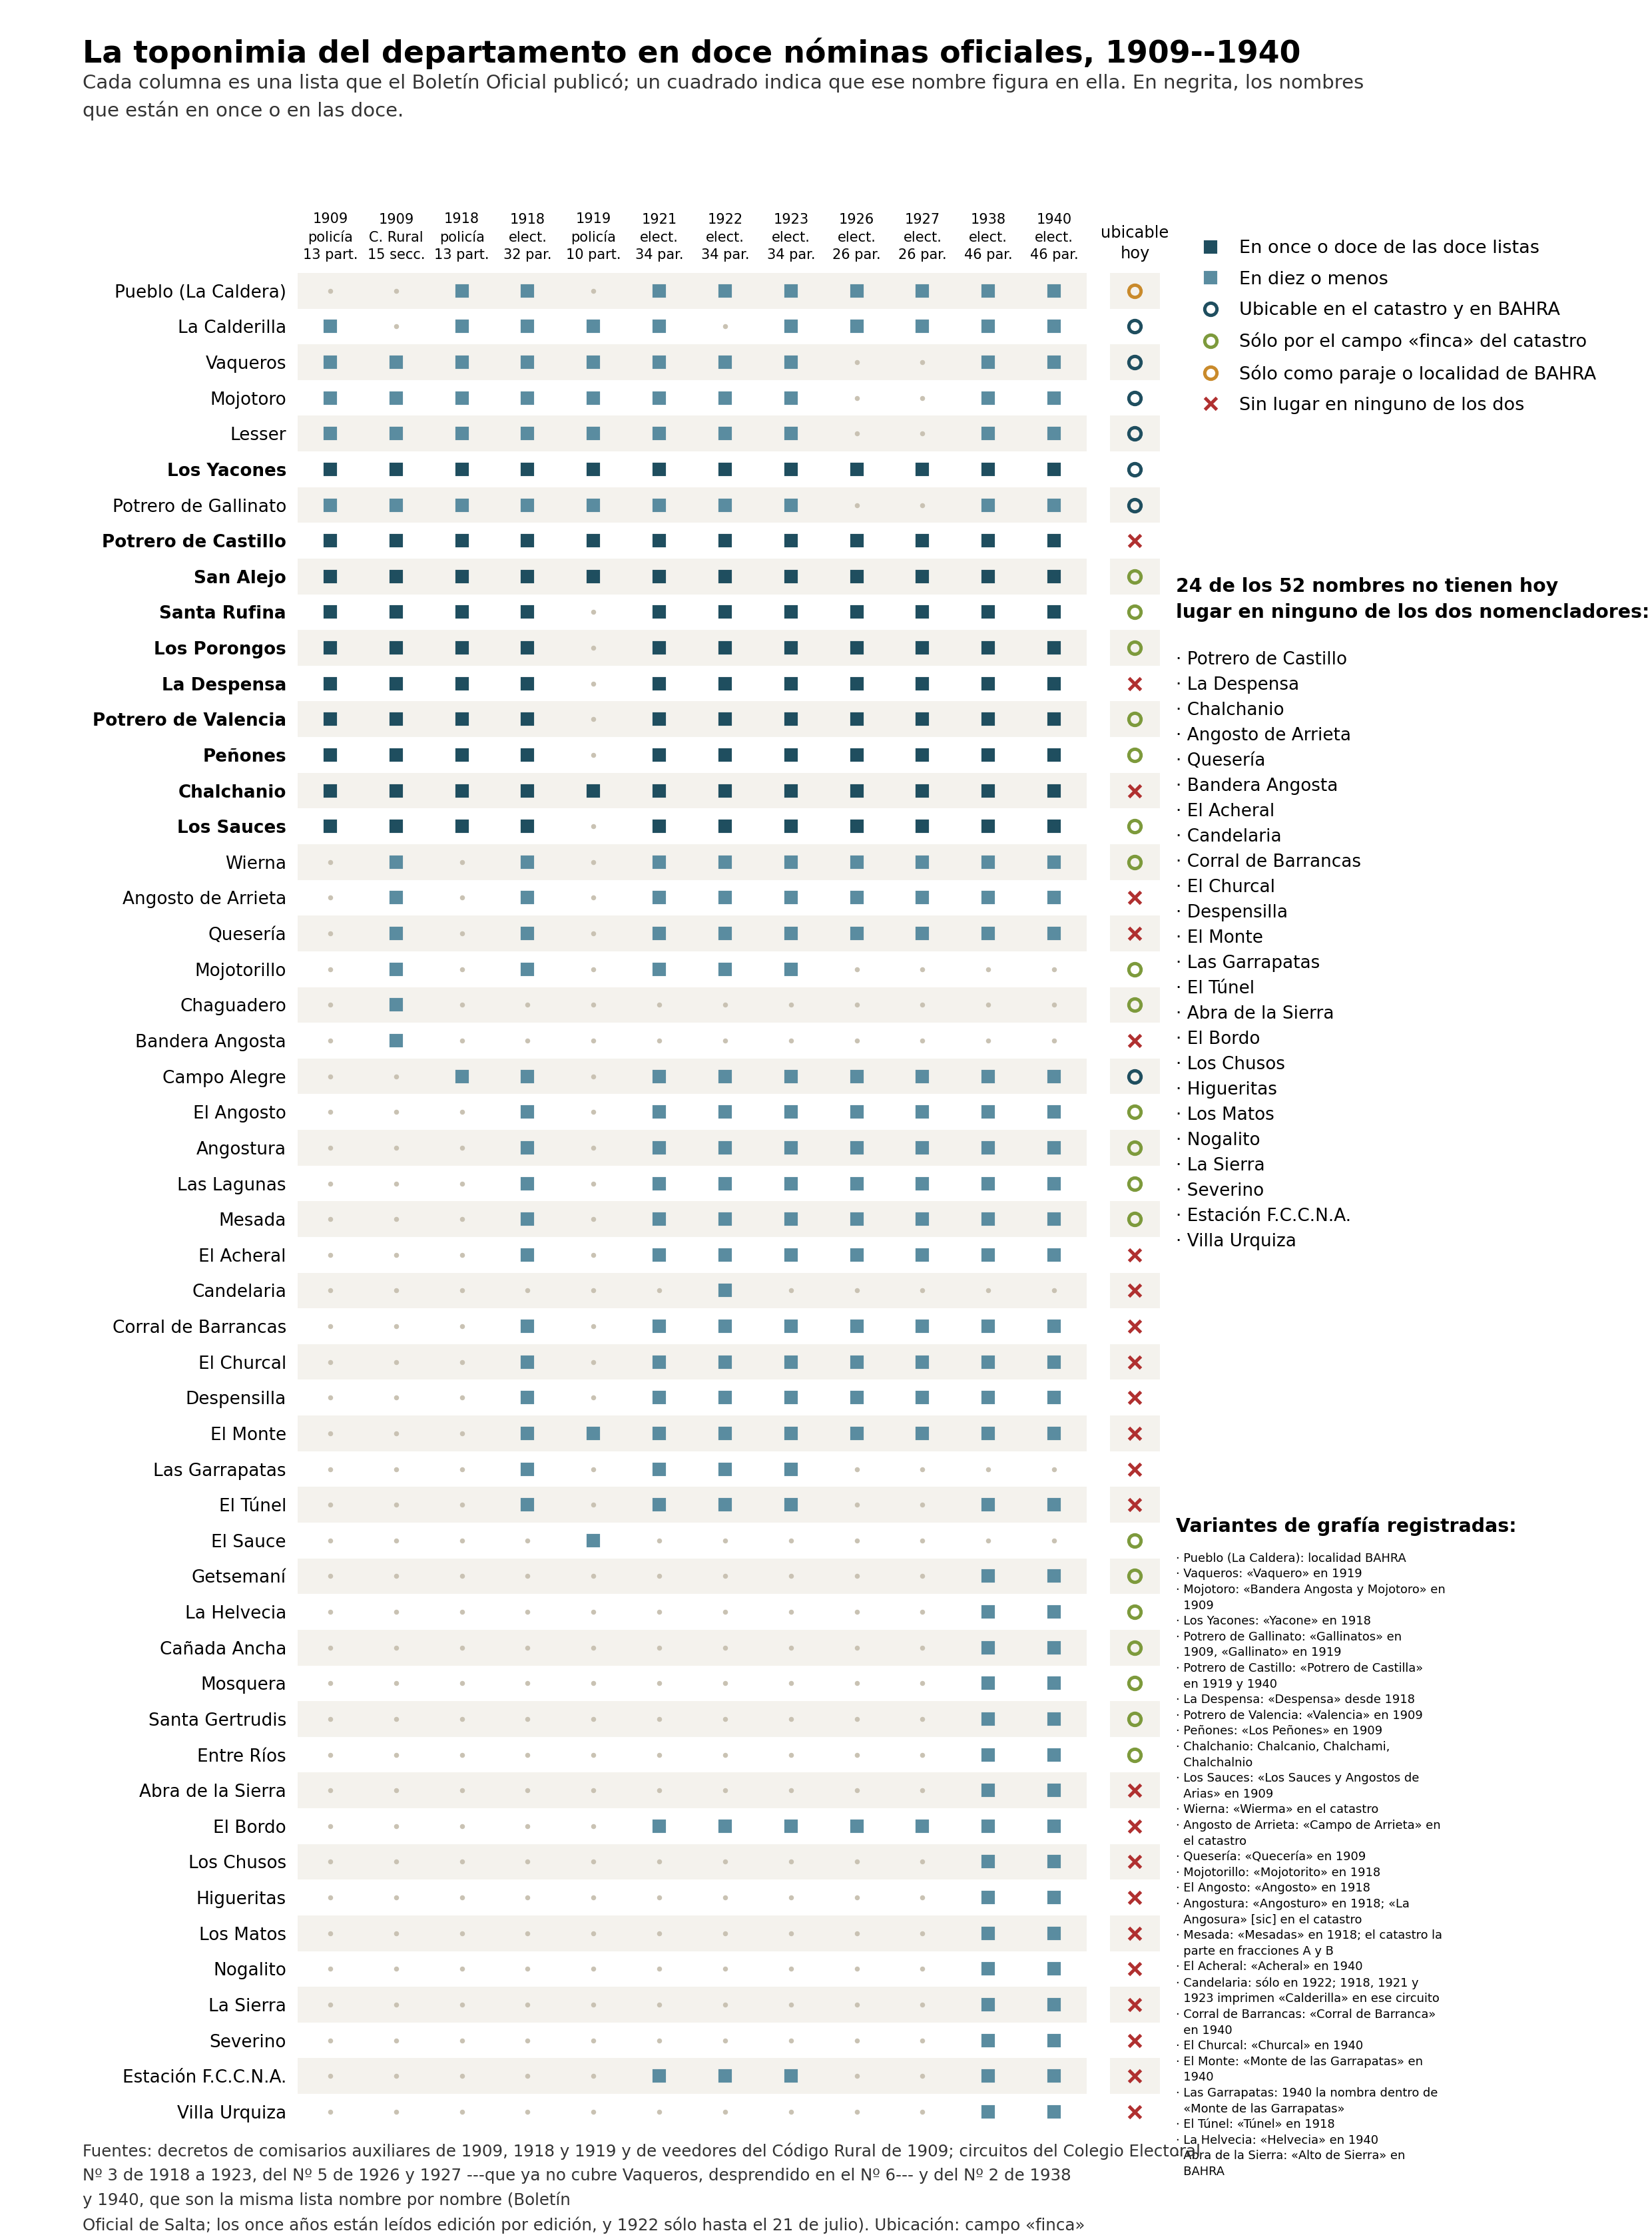
\includegraphics[width=\textwidth,height=0.86\textheight,keepaspectratio]{fig-parajes-nominas.png}
\caption[La toponimia del departamento en doce nóminas oficiales, 1909--1940]{\textbf{La toponimia
del departamento en doce nóminas oficiales, 1909--1940.} Cada columna es una lista que el Boletín
Oficial publicó ---los comisarios auxiliares de policía de 1909, 1918 y 1919, los veedores del
Código Rural de 1909, y los circuitos electorales del Colegio Nº 3 de 1918 a 1923, los del Nº 5 de 1926 y 1927 ---que ya no cubren Vaqueros, desprendido en el Nº 6--- y los del Nº 2 de 1938 y de 1940, que son la misma lista nombre por nombre---; un cuadrado indica que ese
nombre figura en ella. La columna de la derecha dice si el topónimo tiene hoy lugar en el campo
«finca» del catastro parcelario, en la Base de Asentamientos Humanos, en los dos o en ninguno.
Los once años están leídos edición por edición, y 1922 sólo hasta el 21 de julio (apéndice \ref{cap:fuentes}). Elaboración propia
con el catastro parcelario de la Provincia (IDESA, consultado en septiembre de 2026) y BAHRA;
la tabla y el dibujo los produce \texttt{scripts/tabla\_parajes.py} del repositorio
\texttt{mapas\_caldera} (apéndice \ref{cap:fuentes}).}
\label{fig:parajesnom}
\end{figure}

\begin{figure}[p]
\centering
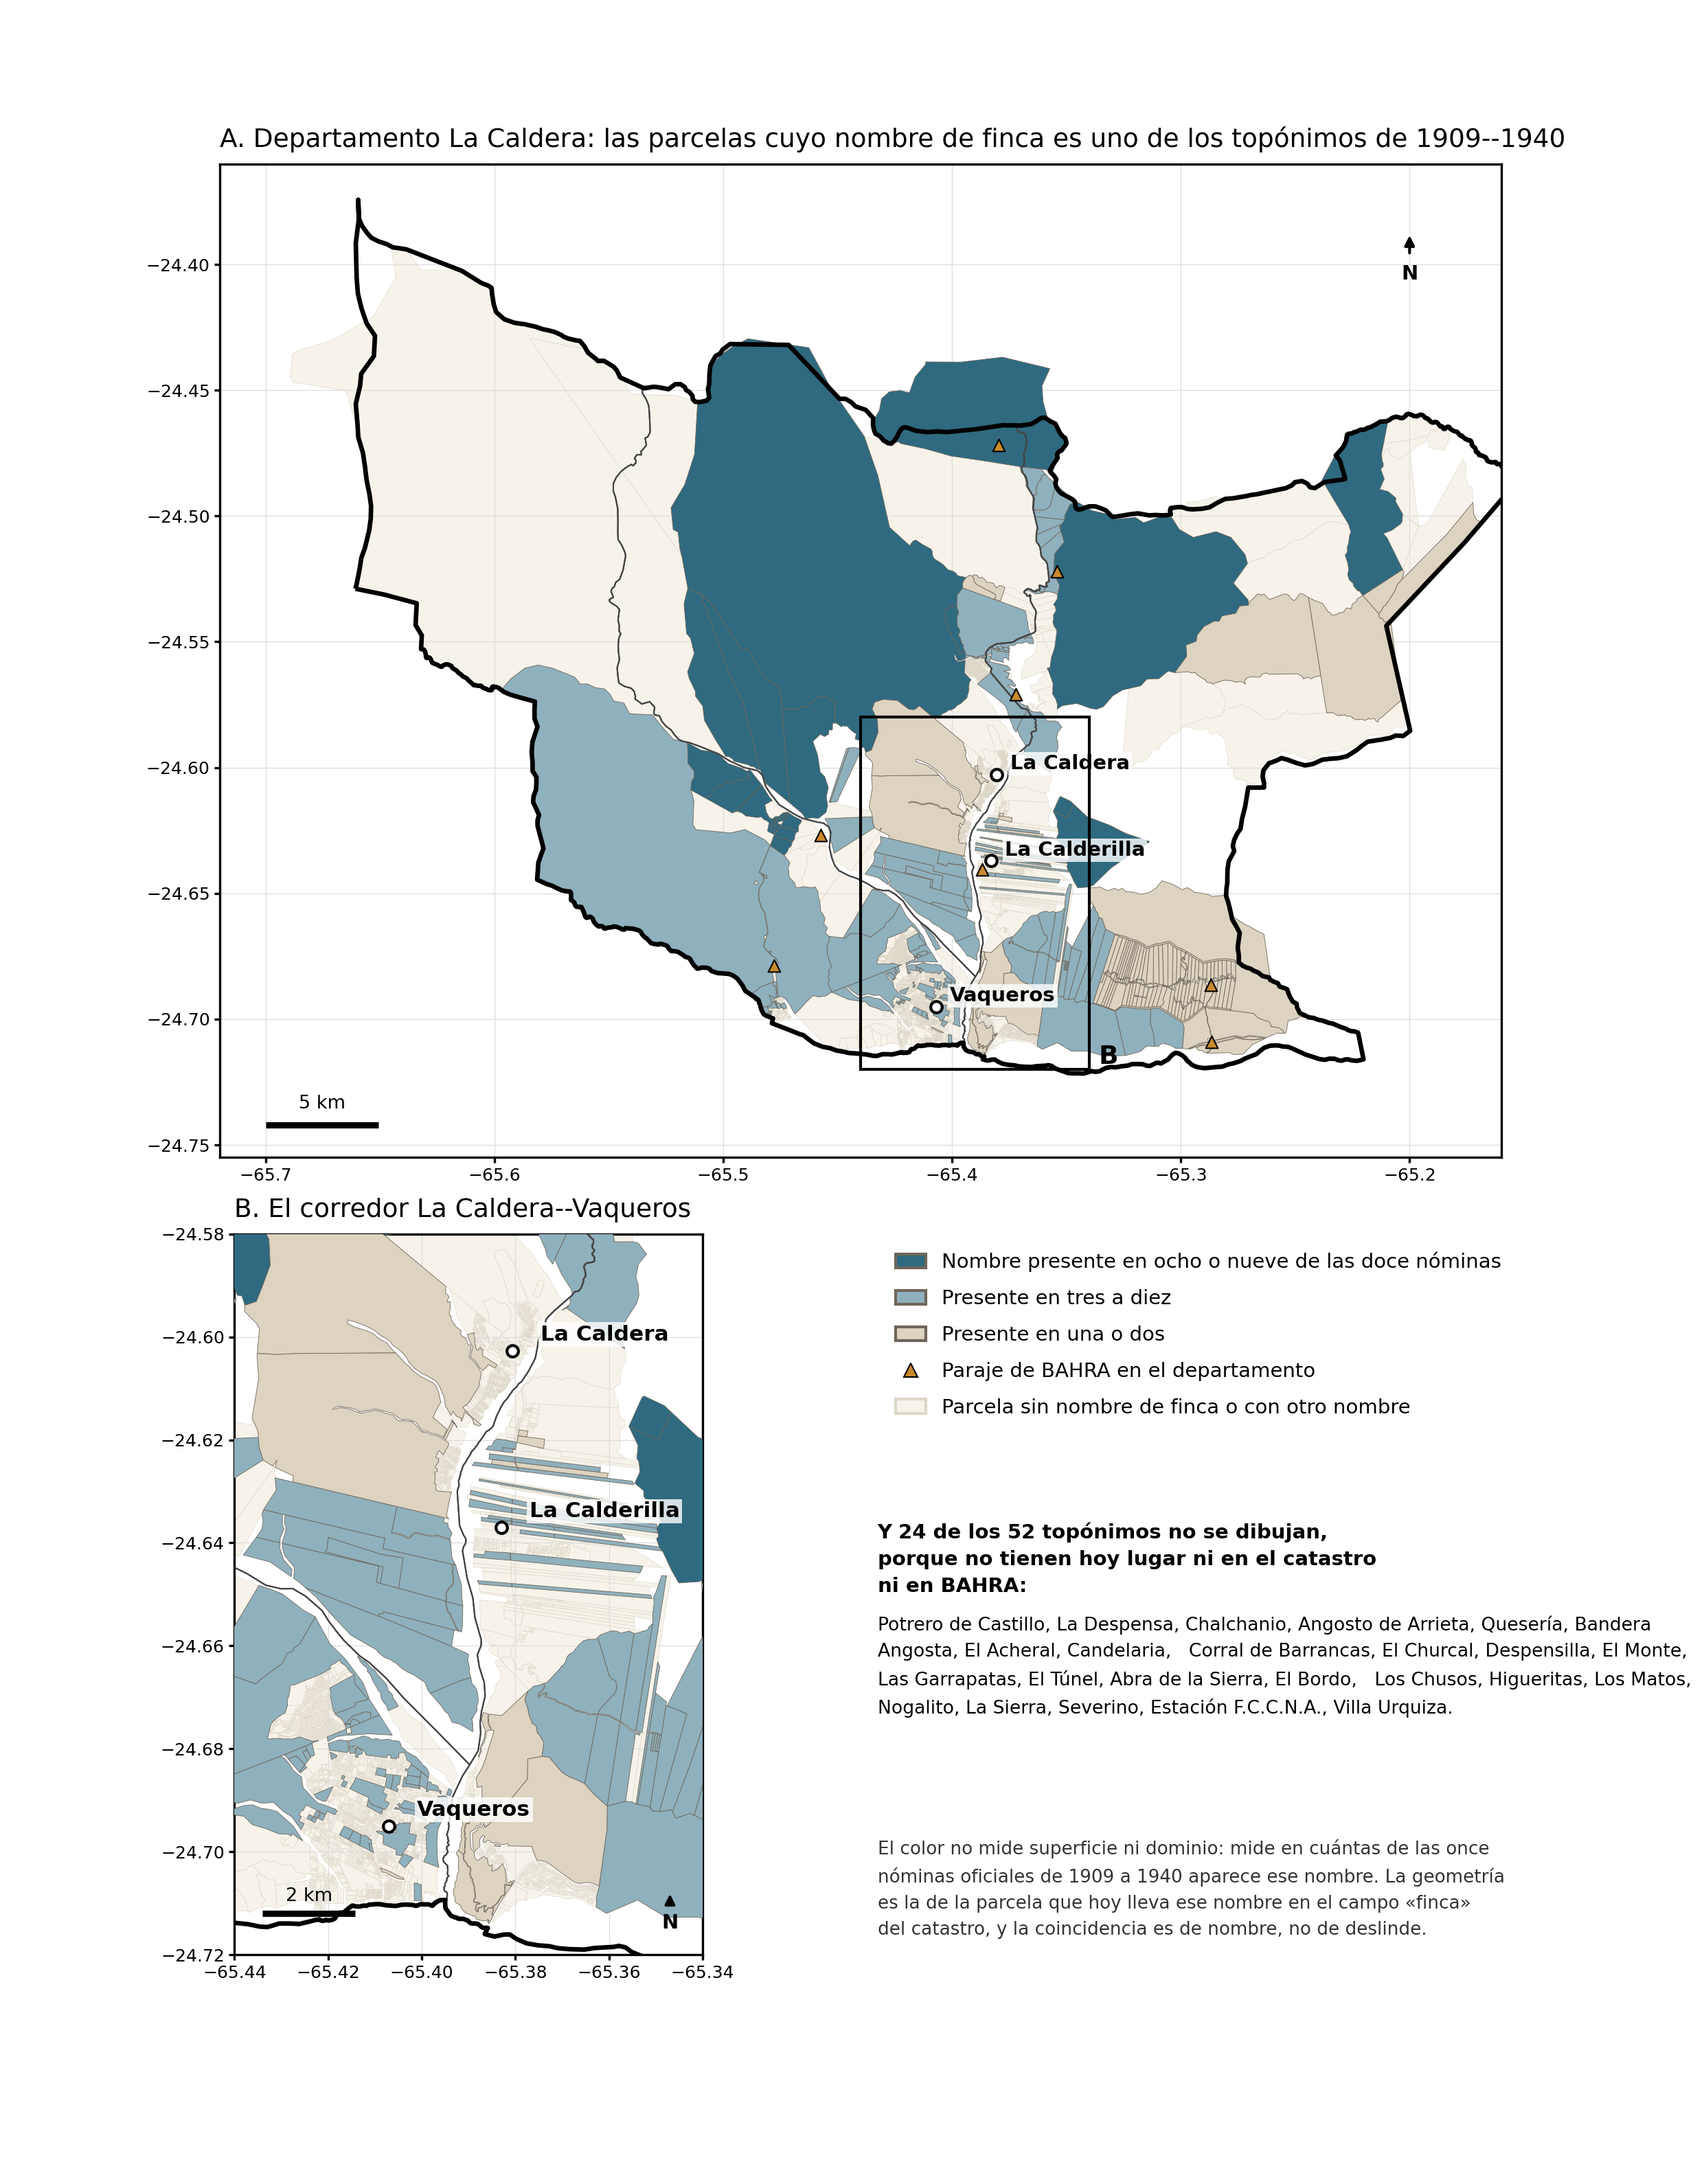
\includegraphics[width=\textwidth,height=0.86\textheight,keepaspectratio]{fig-parajes-mapa.png}
\caption[Dónde caen hoy los topónimos de 1909--1940]{\textbf{Dónde caen hoy los topónimos de
1909--1940.} A: las parcelas cuyo campo «finca» lleva uno de los cincuenta y dos nombres de la
lámina \ref{fig:parajesnom}, coloreadas según en cuántas de las doce nóminas aparece ese nombre;
los triángulos son los parajes que BAHRA registra en el departamento. B: el corredor La
Caldera--Vaqueros. \textbf{El color no mide superficie ni dominio}: mide permanencia en el
registro del Estado. La geometría es la de la parcela que hoy lleva ese nombre, y la coincidencia
es de nombre y no de deslinde. Veinticuatro de los cincuenta y dos topónimos no se dibujan, y se
enumeran en el recuadro. Elaboración propia con el catastro parcelario de la Provincia (IDESA,
consultado en septiembre de 2026), BAHRA y la cartografía de radios del Censo 2022 (INDEC);
dibujo de \texttt{scripts/mapa\_parajes.py} del repositorio \texttt{mapas\_caldera}
(apéndice \ref{cap:fuentes}).}
\label{fig:parajesmapa}
\end{figure}

\subsection*{Doce nóminas del mismo territorio, y lo que queda de ellas}

Entre 1909 y 1940 el Estado provincial publicó \textbf{doce listas} de las unidades en que se
divide este departamento, y \textbf{sólo dos de las doce coinciden entre sí}. Tres son de policía ---los
comisarios auxiliares de 1909, de 1918 y de 1919---, una es del Código Rural ---los veedores de
1909---, y ocho son electorales ---los circuitos de 1918, 1921, 1922, 1923, 1926, 1927, 1938 y 1940---. Las doce
salen de tramos leídos edición por edición, de modo que son la lista entera y no una muestra.

Puestas una al lado de la otra dan \textbf{cincuenta y dos nombres distintos}, y el resultado se
lee de un golpe en la lámina \ref{fig:parajesnom}.

\begin{cautela}
\textbf{Tres cosas se leen ahí, y las tres importan para lo que este libro sostiene.}

\textbf{La primera: hay un núcleo que no se mueve.} \textbf{Diez} nombres aparecen en once o en
las doce listas, con treinta y un años y cuatro autoridades distintas de por medio:
Los Yacones, Potrero de Castillo, San Alejo,
Santa Rufina, Los Porongos, La Despensa, Potrero de Valencia, Peñones, Chalchanio y Los Sauces.
\textbf{Vaqueros, Mojotoro, Lesser y Potrero de Gallinato salieron de esa lista por una sola
razón}: desde 1926 están en el Colegio Electoral Nº 6 y no en el Nº 5, de modo que faltan de las
dos últimas nóminas del Colegio 5 sin haber dejado de existir. \textbf{Son los mismos con los que el capítulo \ref{cap:cot} muestra
que el municipio se describe a sí mismo en el artículo 6.º de su plan de 2015}, cien años después.
\textbf{Y hay un decimoquinto que se cae de esa lista por una sola ausencia}: \textbf{La
Calderilla} está en diez de las doce y falta justamente en la de 1922, donde el mismo circuito
imprime «Candelaria» y donde 1921 y 1923 imprimen Calderilla. Es la discordancia que este capítulo registra más arriba y no resuelve, y
es la única razón por la que el paraje que da nombre a medio departamento no figura entre los
permanentes.

\textbf{La segunda: alrededor de ese núcleo, la división cambia todo el tiempo.} Los veedores del
Código Rural de 1909 usan una partición distinta de la de la policía del mismo año ---aparecen
Wierna, Bandera Angosta, Mojotorillo y Chaguadero, que la lista policial no nombra---; 1918
enumera trece partidos y 1919, diez; y el circuito electoral de 1918 nombra treinta y dos parajes,
el de 1921 treinta y cuatro, el de 1922 otros treinta y cuatro que no son los mismos, el de 1923 los de 1921 otra vez, los de 1926 y 1927 veintiséis cada uno ---sin Vaqueros--- y los de 1938 y 1940 cuarenta y seis, \textbf{que son la misma lista}. \textbf{Ninguna de las siete listas
deslinda nada}: todas
nombran, y el libro no puede saber si lo que cambia es el territorio o la enumeración.

\textbf{Y la tercera, que es la que no se esperaba: veinticuatro de los cincuenta y dos nombres no
tienen hoy lugar en ningún nomenclador.} No están en el campo «finca» del catastro parcelario ni
en la Base de Asentamientos Humanos. Entre ellos hay siete que el circuito electoral de 1918
nombra como lugares donde vive gente que vota ---Despensilla, Corral de Barrancas, El Churcal, El
Monte, Las Garrapatas, El Túnel y La Despensa---, y nombres que los circuitos de 1921 y el padrón de 1940 todavía
registraban, como El Bordo, la Estación del ferrocarril, Severino, Los Chusos, Higueritas, Los
Matos y Nogalito. \textbf{Una parte de la toponimia con la que el Estado organizaba el voto y la
policía de este departamento se borró del registro oficial sin que ningún acto lo dispusiera}, y
el capítulo \ref{cap:ausencias} la retoma como lo que es: una ausencia medida.
\end{cautela}

\begin{cautela}
\textbf{Qué prueba la lámina \ref{fig:parajesmapa} y qué no.} Prueba que veintiocho de los
cincuenta y dos topónimos siguen teniendo una geometría asociada, y dónde caen. \textbf{No prueba
que esa geometría sea la de entonces}: la coincidencia es de nombre y no de deslinde, y el
catastro no dice si los límites actuales son los de 1909. Por eso el mapa no dibuja polígonos de
partido: \textbf{ninguno de los siete instrumentos deslinda las unidades que nombra}, y trazar sus
límites sería inventar una frontera que el archivo no da. Esa correspondencia entre los nombres y
las matrículas actuales es, exactamente, lo que el apéndice \ref{cap:pedidos} reclama a la
Dirección General de Inmuebles.
\end{cautela}

\subsection*{Y 1920 es un año de una sola plaza y de una elección}

El año 1920 se leyó también edición por edición y es el décimo tramo: las ediciones 788 a 839,
48 ediciones, 526 hojas distintas sobre seiscientos folios (apéndice \ref{cap:fuentes}). Dejó
diez actos del departamento, ninguno de dominio, y se reparte en dos materias y nada más: una
plaza de policía y una elección.

\subsubsection*{La plaza que se creó en 1919 rota tres veces en 1920}

En septiembre de 1919 el decreto 522 creó la Sub-Comisaría de Mojotoro «\textit{con sueldo}».
\textbf{En 1920 el puesto cambia de manos tres veces}, y ninguno de los tres decretos cita al
anterior:

\begin{ficha}{El puesto de Sub-Comisario de Mojotoro en 1920}
\textbf{Decreto N.\ 677, 4 de febrero.} Acepta la renuncia de \textbf{Silverio Cáceres},
«\textit{del puesto de Sub Comisario de Policía de Mojotoro, jurisdicción del Departamento de la
Caldera}». No dice quién lo reemplaza. \textit{(B.O.\ Nº 795.)}

\textbf{Decreto N.\ 724, 26 de febrero.} Nombra a \textbf{José Agustín Martínez} «\textit{para
ocupar el puesto vacante de Sub-Comisario de Mojotoro, \textbf{partido} del departamento de la
Caldera}», a propuesta de la Jefatura de Policía. \textbf{No menciona la renuncia que el propio
Boletín había publicado tres semanas antes.} \textit{(B.O.\ Nº 798.)}

\textbf{Decreto N.\ 901, 16 de junio.} Nombra a \textbf{Ciro Cáceres} Sub-Comisario de Policía de
Mojotoro, «\textit{Departamento de La Caldera}», por la nota N.\ 1.622 M.-19 de la Jefatura de
Policía, que no se publica. \textbf{Tampoco dice que Martínez haya renunciado ni lo nombra}: la
vacante se declara sin nombrar a quien la dejó. \textit{(B.O.\ Nº 816.)}
\end{ficha}

\begin{cautela}
\textbf{Tres cosas se leen ahí.}

\textbf{La primera es la rotación.} La única plaza rentada de policía \textbf{de partido} que el
departamento consiguió en toda esta serie ---la comisaría departamental sí estaba presupuestada,
y el ítem V de 1919 paga una treintena de comisarios de campaña, según cuál de las dos lecturas del renglón se tome--- duró cuatro meses y medio en manos de su primer titular y tres meses y medio en las del segundo
---si es que Martínez llegó a tomar posesión, cosa que el Boletín no publica---. Entre la renuncia
del primero y el nombramiento del segundo pasaron tres semanas.

\textbf{La segunda es de forma, y es la que interesa a este libro.} De los tres decretos, dos
\textbf{declaran una vacante sin nombrar a quien la dejó}. El acto dice que el puesto está vacante
y no dice por qué ni desde cuándo. Es el mismo mecanismo que el capítulo \ref{cap:opacidad}
describe cien años después con otro contenido: lo publicado permite saber que algo se decidió y
no qué se decidió.

\textbf{Y la tercera es de nombre.} La misma unidad se llama «\textit{jurisdicción del
Departamento}» en febrero y «\textit{partido del departamento}» tres semanas después, en dos
decretos del mismo gobierno. La nómina de partidos que 1909, 1918 y 1919 publican cada año deja
de publicarse: \textbf{1920 no trae lista de partidos}, y Mojotoro aparece solo.
\end{cautela}

\textbf{Y en octubre se cubre el registro civil, también sobre una vacante sin dueño.} El decreto
N.\ 1140 del 25 de octubre nombra encargado de la Oficina del Registro Civil de La Caldera a
\textbf{Casimiro Cáceres} ---el mismo que fue juez de paz propietario del departamento en 1918 y
en 1919--- «\textit{con antigüedad al 5 de Agosto ppdo.\ fecha desde la cual presta servicios en
carácter de interino}». \textbf{El interinato que el decreto reconoce nunca se publicó}, y la
vacante se declara otra vez sin nombrar a quien la dejó.

\subsubsection*{La elección de 1920, y un departamento que figura dos veces}

Nueve de las dieciséis apariciones del año son electorales. La convocatoria es del 6 de febrero,
para el comicio del 7 de marzo, y trae un dato que conviene poner entero porque no se concilia.

\begin{ficha}{Decreto N.\ 685 --- Salta, 6 de febrero de 1920}
«\textit{Art.\ 1.º---Convócase al pueblo de la Provincia a elecciones de Senadores y Diputados
provinciales, que se llevará a cabo el 7 de Marzo próximo en la siguiente forma: Por la Capital
cinco Diputados; Molinos un Diputado; \textbf{Caldera un Diputado}; Cafayate un Senador;
Guachipas un Diputado; Chicoana dos Diputados; Metán un Diputado; Cerrillos un Diputado;
\textbf{Caldera un Diputado}; Rivadavia dos Diputados y un Senador; Iruya un Diputado; Orán dos
Diputados; Rosario de Lerma, dos Diputados}».
\textit{(B.O.\ Nº 795, h.\ 5 y 6, pág.\ 1.136.)}
\end{ficha}

\begin{cautela}
\textbf{Caldera figura dos veces en la misma enumeración, con la misma grafía y con un diputado
cada vez.} Está confirmado en la imagen y se transcribe como está. Este libro \textbf{no concilia}
y no infiere que la segunda mención deba decir otro departamento.

Y la lista es además \textbf{parcial}: no nombra a La Viña, Anta, Campo Santo, Rosario de la
Frontera, La Candelaria, San Carlos, Cachi ni Santa Victoria. \textbf{Un acto que convoca a toda
la provincia a votar enumera doce departamentos distintos en trece renglones}, repite uno y deja
sin nombrar al menos ocho.

No se saca de ahí ninguna conclusión sobre la representación del departamento: se registra que el
instrumento que la fija, ese año, no cierra consigo mismo.
\end{cautela}

\textbf{Las cuatro mesas son las mismas de 1918.} El mismo decreto ubica el Colegio Electoral
N.\ 3 de Caldera en cuatro puntos: la \textbf{Escuela Elemental Mixta} y la \textbf{Iglesia
Parroquial} del pueblo, la \textbf{Escuela Infantil Provincial} de Vaqueros y la \textbf{Oficina
de Correos} de Mojotoro. Son los cuatro edificios de 1918, dos años después y sin variación. Lo
que 1920 \textbf{no} publica son los circuitos: los treinta y dos parajes que 1918 enumeraba uno
por uno no vuelven a aparecer (lámina \ref{fig:parajesnom}).

\textbf{Tres partidos proclamaron candidato por el departamento}, y el tercero es un nombre
conocido: por la Unión Cívica Radical Intransigente, \textbf{José María Ocaranza}; por la Unión
Provincial, \textbf{José Antonio Aráoz}; y por la Unión Cívica Radical, \textbf{Dermidio
Arancibia}.

\begin{cautela}
\textbf{Dermidio Arancibia es, dos años antes, uno de los dos descubridores de las minas del
departamento.} El aviso de julio de 1918 lo nombra, junto con Miguel A.\ Sosa, como peticionante
de la mina de plomo «20 de Febrero» en la finca Cerro Nevado, y en agosto los dos denuncian el
despueble de la mina «Sara». En 1920 es candidato a diputado por el mismo departamento.

\textbf{Coincidencia de nombre, como siempre, y no identificación registral.} Pero si es la misma
persona, es el primer caso documentado en esta serie de alguien que pide una concesión sobre el
suelo del departamento y se presenta a representarlo, y el capítulo \ref{cap:politica} lo retoma
donde corresponde.
\end{cautela}

\textbf{Y a Augusto Regis lo sacan de la mesa antes de votar.} La nómina de la Junta Electoral de
febrero registra, para el Colegio Electoral N.\ 3 de Caldera, mesa N.\ 1: «\textit{Pte.,
Fernández Alberto Tomás, en reemplazo de Regis Augusto}»\index{Regis, Augusto}. El mismo Augusto
Regis que este libro sigue desde 1908 y que en 1918 era segundo suplente de esa misma mesa. El
acto no dice por qué.

\textbf{Y la urna del departamento se anuló.} El decreto N.\ 772 del 22 de marzo convoca a
elecciones complementarias para el 4 de abril «\textit{de las urnas que han sido anuladas}», y la
primera de la lista es «\textit{La Caldera --- C.\ Electoral N.º 3 Mesa N.º 4}».

\begin{cautela}
\textbf{La mesa 4 es la de Mojotoro}, según el decreto de febrero que ubica las cuatro. El decreto
772 no lo dice: nombra el colegio y el número de mesa, no el lugar, \textbf{y el cruce lo hace
este libro}. Tampoco dice por qué se anuló.

Puesto junto al resto del año, el cuadro es éste: la única plaza rentada de policía de partido del
departamento está en Mojotoro y cambia de manos tres veces en cinco meses; la única urna anulada
del departamento es la de Mojotoro; y ninguno de los dos actos explica nada. \textbf{Este libro no
afirma que haya relación entre las dos cosas}, y lo deja anotado porque el que siga puede
buscarla.
\end{cautela}

\textbf{Cierra el año un nombramiento militar.} Un decreto en acuerdo de Ministros de noviembre
nombra Coroneles de la Guardia Nacional por departamento; por Caldera, \textbf{Mariano Coll}. El
artículo 2.º nombra tenientes coroneles sólo por cinco departamentos, y Caldera no está entre
ellos.

\begin{cautela}
\textbf{Un año sin una sola cifra del departamento.} 1920 publica \textbf{diez resúmenes del
movimiento de la Tesorería General}, más que ningún otro de los años cuyos resúmenes este libro
contó uno por uno ---1911 publicó uno, 1912 cuatro, 1918 tres y 1919 ninguno; del tramo 1923--1946
no hay recuento---, y el propio Boletín los encadena mes a mes por la existencia de caja. \textbf{Y
no publica un solo balance municipal}, ni de este departamento ni de ningún otro. El Estado
provincial rinde su caja diez veces en un año; los municipios, ninguna (apéndice
\ref{cap:fuentes}).
\end{cautela}

\subsection*{Y 1921 devuelve los deslindes, y devuelve a los mismos linderos}

El año 1921 se leyó también edición por edición y es el undécimo tramo: las ediciones 840 a 888,
de las que seis son marcadores de ausencia del repositorio, de modo que son 43 ediciones y 742
hojas (apéndice \ref{cap:fuentes}). Dejó dieciocho actos del departamento, y \textbf{dos de ellos
son de dominio: los primeros desde 1917}, después de tres años seguidos en cero.

\begin{ficha}{Deslinde de la finca «El Angosto» --- B.O.\ Nº 869, 19 de agosto de 1921, aviso Nº 286}
Se presenta el procurador Elías Gallardo «\textit{con poder y títulos bastantes}» de la señora
\textbf{Antonia P.\ de Peralta} pidiendo el deslinde, mensura y amojonamiento de la finca «El
Angosto», departamento de La Caldera,

\begin{quote}
«\textit{limitada al Norte, propiedad de los herederos de \textbf{Luisa A.\ Costas}, hoy
\textbf{Daniel Linares} y de \textbf{Julio Mercado}; al Sud, el monte del \textbf{Quitilipe}
separado por el río de La Caldera y propiedad de \textbf{Susana Aguilera}; al Este, propiedad de
\textbf{Augusto Reyes}; al Oeste, herederos de \textbf{Luis A.\ Costas} \textit{[sic]} hoy Daniel
Linares}».
\end{quote}

Juez Alberto Mendioroz, agrimensor Rodolfo Chávez, secretario Tomás Izarrualde.
\end{ficha}

\begin{cautela}
\textbf{Los tres linderos del este, del sud y del norte son los mismos de 1909.} El remate de una
décima parte indivisa del \textbf{Angosto de Arrieta}, publicado en 1909, declara como linderos
«\textit{al este Julio Mercado, Augusto Rejis\index{Regis, Augusto} y Susana Aguilera}» (apéndice
\ref{cap:dominio}). \textbf{Doce años después, sobre el paraje contiguo, vuelven los tres
nombres}: Julio Mercado al norte, Susana Aguilera al sud y un Augusto ---impreso Reyes en 1921 y
Rejis en 1909--- al este.

\textbf{Este libro no unifica Reyes con Rejis ni afirma que las dos fincas sean la misma.} Lo que
queda establecido es que \textbf{la vecindad de propietarios del sector del Angosto no cambió en
doce años}, y que uno de ellos ---Julio Mercado--- es, en 1919 y en 1928, miembro de la Comisión
Municipal del departamento. Es la tercera tesis en su forma más literal: las unidades y los
nombres duran.

\textbf{Y aparece Quitilipe}, que el archivo registra en 1912 y otra vez en 1916, las dos en el
deslinde de «Santa Mónica y Quitilipe», y que aquí es el monte del sud, separado por el río. \textbf{Y aparece Daniel
Linares}\index{Linares, Daniel}, que en 1917 era miembro de la comisión municipal y candidato a
diputado, ahora como propietario en dos de los cuatro rumbos.

\textbf{Una errata del propio edicto que no se concilia}: el mismo texto escribe «Luisa A.
Costas» en el lindero del norte y «Luis A.\ Costas» en el del oeste. Dos personas o una sola mal
impresa.
\end{cautela}

\textbf{Y el segundo deslinde del año es el que este libro ya tenía, ahora con su edición.} El
edicto de «\textbf{Cerro de Buena Vista}» y «\textbf{Sausal o Curuzú}», partido de Vaqueros, de
Francisco S.\ Urquiza\index{Urquiza, Francisco S.}, sale en la edición 843 del 28 de enero. El
barrido agrega tres cosas: el juez es Daniel Etcheverry y el secretario Tomás Izarrualde; la
resolución se imprime «\textit{Salta, Octubre 18 de 1020}» \textit{[sic]}, con un cero donde la
fecha pide un nueve; y el auto ordena publicar el edicto \textbf{treinta días en dos diarios y
«\textit{por una sola vez}» en el Boletín Oficial}.

\begin{cautela}
\textbf{Esa instrucción vale más que el edicto.} En 1921 un juez de primera instancia distingue,
en el mismo auto, la publicación que da noticia ---treinta días en dos diarios de la capital---
de la que deja constancia ---una sola vez en el Boletín---. \textbf{El Boletín no es, en esta
época, el lugar donde se entera el interesado}: es el lugar donde queda el acto.

Cien años después, el capítulo \ref{cap:ribera} documenta líneas de ribera que salen dos días en
el Boletín y no se asientan en la matrícula, y el capítulo \ref{cap:opacidad} lo llama el canal:
la información existe, se publica y no viaja por donde mira el interesado. \textbf{En 1921 el
juez lo sabía y por eso mandaba las dos publicaciones.}
\end{cautela}

\subsection*{Un distrito cuya elección se anula entera}

De los dieciocho actos del año, nueve son electorales, y la serie termina mal.

\begin{ficha}{Decreto N.\ 1828 --- Salta, 20 de septiembre de 1921}
«\textit{Habiendo comunicado el señor Presidente de la Junta Electoral de la Provincia, en nota
N.o 30 de fecha 6 del corriente, que dicha Junta ha resuelto \textbf{declarar nula la elección
practicada el día 7 de Agosto ppdo., en los distritos eleectorales} \textit{[sic]} \textbf{de la
Caldera}, Rosario de Lerma, Rosario de la Frontera, La Candelaria, Guachipas, Iruya, Anta, Metán,
Santa Victoria, San Carlos, Orán y Rivadavia, \textbf{por no haberse verificado elección legal en
dos tercios de las mesas}}» ---artículos 75 y 84 de la Ley de Elecciones---, se convoca de nuevo
para el segundo domingo de octubre. A Caldera le corresponden \textbf{dos Convencionales para la
reforma de la Constitución}.
\textit{(B.O.\ Nº 879, 28 de octubre de 1921, h.\ 15 y 16.)}
\end{ficha}

\begin{cautela}
\textbf{Dos años seguidos con la elección del departamento anulada.} En 1920 se anuló una urna
---la de la mesa 4, que es la de Mojotoro--- y hubo complementarias. En 1921 se anula
\textbf{toda la elección del distrito}, y no por un incidente sino porque no hubo elección legal
en dos tercios de las mesas. El departamento no está solo: son doce distritos de los veintidós.

\textbf{Y la convocatoria a la nueva elección se publica el 28 de octubre, diecinueve días después
del segundo domingo de octubre, que cayó el 9.} El Boletín publica la citación cuando la fecha
señalada ya pasó. El decreto es del 20 de septiembre y la nota que lo funda, del 6: cincuenta y
dos días entre la resolución y su publicidad.

Este libro \textbf{no puede decir si la elección de octubre se hizo}, ni con qué convocatoria, ni
qué pasó con los dos convencionales del departamento en la reforma constitucional. Ni la nota N.\
30 de la Junta ni la resolución que declara la nulidad se publican, y los dos quedan pedidos en
el apéndice \ref{cap:pedidos}.
\end{cautela}

\textbf{Y el año trae cuatro nóminas de autoridades y de candidatos.} En febrero la Unión Cívica
Radical proclama por La Caldera al senador \textbf{Emeterio Royo} y al diputado \textbf{Lucio
Ortiz}; en diciembre, para el comicio de enero de 1922, la Unión Provincial proclama a
\textbf{José Antonio Aráoz} ---el mismo candidato que presentó en 1920--- y la Unión Cívica
Radical a \textbf{Natal López Cross}. Las autoridades de mesa de febrero y las de diciembre
traen veinticuatro nombres, y entre ellos vuelven \textbf{Domingo Royo}, \textbf{Daniel
Linares}\index{Linares, Daniel}, \textbf{Enrique J.\ Rauch}, \textbf{Gregorio Nogales},
\textbf{Nolasco Echenique} y \textbf{Eustaquio Murúa}\index{Murúa, Eustaquio}, que preside la
mesa 1 en diciembre.

\subsection*{Y Escolástico Aparicio vuelve, y dura dos meses}

El capítulo daba por cerrada en 1918 la serie de \textbf{Escolástico M.\
Aparicio}\index{Aparicio, Escolástico M.}, cuando la Intervención lo trasladó de la Receptoría de
Caldera a la de Campo Santo. \textbf{Vuelve en 1921}: el decreto 1669 del 7 de julio lo nombra
Juez de Paz Suplente del departamento, «\textit{vistas las ternas elevadas por la Comisión
Municipal del Departamento de la Caldera}», con \textbf{Laureano Peralta} de propietario. Y el
decreto 1816 del 12 de septiembre acepta su renuncia, «\textit{en atención a los motivos en que
la funda}», que el decreto no transcribe.

\begin{cautela}
\textbf{Dos meses y cinco días}, y el acto no nombra reemplazante: en lo que queda del año no se
publica otro que cubra esa vacante. \textbf{Y es la primera vacante sin destino de la serie}: las
tres que 1920 dejó eran del signo contrario ---declaraban el hueco sin nombrar a quien lo
dejaba---, y ésta nombra al que se va y no al que entra. El mismo año trae las dos formas: el
decreto 1669 que lo nombra tampoco dice quiénes eran los jueces salientes.

\textbf{Y el decreto que lo nombra tampoco nombra a los salientes} ni cita el acto por el que
cesaron: el visto habla de ternas para cubrir los cargos y no dice quién los dejaba. \textbf{Doce
años de cargos del departamento, y el archivo no permite armar la sucesión completa de ninguno de
ellos.}
\end{cautela}

\textbf{Y en noviembre un vecino pierde dos cargos en cuatro días.} El decreto 2021 del 7 declara
cesante al Comisario de Policía de La Caldera, \textbf{don Julio Royo}, y nombra «\textit{al
Ernesto Tedin}» \textit{[sic]}; el decreto 2062 del 11 lo separa del cargo de \textbf{Receptor de
Rentas y Expendedor de Guías} del departamento «\textit{por razones de mejor servicio}» y nombra
a \textbf{Ernesto J.\ Tedin}, con fianza de doña Encarnación Tedin de López por cinco mil pesos.

\begin{cautela}
\textbf{Los dos cargos del departamento que manejan dinero y fuerza pública pasan, en cuatro
días, del mismo hombre al mismo hombre}, y la fianza la da alguien del mismo apellido que el
entrante. El segundo decreto no cita al primero y ninguno de los dos da la causa: «razones de
mejor servicio» es la fórmula. Este libro no infiere nada sobre la conducta de nadie y registra
la operación.

\textbf{Y hay tres Royo en el departamento ese año}: Julio, el cesante; \textbf{Domingo}, miembro
de la Comisión Municipal en 1919 y presidente de la mesa 2 en febrero de 1921; y
\textbf{Emeterio}, candidato a senador por el departamento en la lista radical de febrero. No se
afirma parentesco.
\end{cautela}

\subsection*{Y por fin las escuelas tienen dotación}

El presupuesto de sueldos de las escuelas de la campaña, publicado en noviembre, trae el
departamento entero en dos renglones.

\begin{ficha}{Presupuesto de escuelas de la campaña --- B.O.\ Nº 883, 25 de noviembre de 1921, h.\ 10}
\textbf{Departamento Caldera.} Escuela \textbf{Elemental de 2.\textsuperscript{a}}, Parroquia:
director \$125 y dos maestros de grado a \$110 cada uno, \$345 mensuales y \$1.035 por trimestre.
Escuela \textbf{Infantil de 2.\textsuperscript{a}}, Vaqueros: director \$110 y un maestro \$100,
\$210 mensuales y \$630 por trimestre.
\end{ficha}

\begin{cautela}
\textbf{Es el primer dato de dotación escolar del departamento que este relevamiento encuentra}, y
dice tres cosas. Que el departamento tenía \textbf{dos escuelas} y cinco cargos docentes en total.
Que la del pueblo funcionaba en la \textbf{Parroquia}, que es también una de las cuatro mesas
electorales del departamento desde 1918. Y que \textbf{Vaqueros tenía la suya}, la Escuela
Infantil Provincial, que es la tercera mesa.

Los dos subtotales cierran: 125 más 220 son 345, y 110 más 100 son 210; y la segunda columna es
el trimestre, porque 345 por tres da 1.035 y 210 por tres da 630, igual que en los cuatro ítems
vecinos de la misma hoja.

El capítulo \ref{cap:ausencias} registra la escuela como una de las dimensiones que este libro no
cubre. \textbf{Sigue sin cubrirla}: esto es un renglón de presupuesto, no una historia de la
escuela. Pero con la jubilación de Juana Luque en 1918 y estos dos renglones de 1921, el
departamento deja de ser, en materia escolar, una página en blanco.
\end{cautela}

\section{La primera concesión de agua}

En enero de 1924 la Provincia otorgó una concesión de agua en el departamento. Los
considerandos explican, sin proponérselo, casi todo lo que este libro discute noventa años
después. \textbf{Y el barrido de 1923 aportó, al cierre, la pieza que falta antes del decreto:
el escrito con que el interesado la pidió}, publicado por edicto el 28 de diciembre de 1923.

\begin{ficha}{Pedido de concesión de agua --- B.O.\ Nº 990, 28 de diciembre de 1923, h.\ 13 y 14 (aviso 437)}
«\textit{Salta, Diciembre 10 de 1922.\ ---Francisco S.\ Urquiza}\index{Urquiza, Francisco S.},
con domicilio en Balcarce 415, expone que «\textit{según resulta del título que acompaño poseo
un bien raíz situado en el departamento de la Caldera, \textbf{partido de Vaqueros}, denominado
«Cerro de Buena Vista»}», y pide «\textit{hacer uso de los sobrantes de agua del \textbf{Río de
Wierna}}» en cantidad de \textbf{cien litros por segundo}, «\textit{siendo la extensión que me
propongo regar de \textbf{ciento noventa hectáreas}}».

Acompaña «\textit{un croquis explicativo del recorrido de la acequia}», que arranca del río y
sigue «\textit{por el curso actual de la acequia de la \textbf{finca Vaqueros}, al Oeste del
camino nacional de ésta a Jujuy}»; la única obra de arte necesaria es «\textit{un sifón que
atraviesa el cauce de un río seco que a veces recoge las corrientes veraniegas}». Y declara que
la acequia «\textit{atraviesa únicamente la finca nombrada de propiedad de \textbf{los herederos
Toranzos y doctor Carlos Serrey}}».

Pide, por último, «\textit{se recabe informes de la Municipalidad de la Caldera y se publique
edictos a fin de que los que se crean lesionados en sus derechos hagan valer su oposición en
forma}».

\textbf{Providencia del Ministerio de Gobierno, 12 de enero de 1923:} «\textit{de acuerdo a lo
que prescribe el Código Rural en su artículo 112, inciso 5º, publíquese durante treinta días en
el diario \textbf{La Provincia}}». Firma Ortelli.
\end{ficha}

\begin{cautela}
\textbf{Cinco cosas que el decreto de 1924 no dejaba ver.}

\textbf{Primera: la superficie.} Cien litros por segundo para \textbf{ciento noventa hectáreas}.
El decreto concede el caudal y no dice para cuánta tierra; el pedido sí. Es la primera
equivalencia entre agua y superficie que este libro tiene para el departamento.

\textbf{Segunda: el croquis existe y no se publicó.} El escrito dice acompañarlo y el Boletín
no lo trae ---igual que el plano de Hessling de 1911 y que los anexos que el capítulo
\ref{cap:opacidad} inventaría cien años después---. Citado y no acompañado.

\textbf{Tercera: la acequia atraviesa tierra ajena, y el dueño es un senador.} El propio escrito
declara que el canal cruza la finca Vaqueros «de propiedad de los herederos Toranzos y doctor
\textbf{Carlos Serrey}»\index{Serrey, Carlos}. Cinco meses después, en mayo de 1923, ese mismo
Carlos Serrey se incorpora al Senado provincial \textbf{como senador por Cerrillos}, en la misma
nómina que trae al senador por Caldera. \textbf{Coincidencia de nombre y no identificación
registral}; si es la misma persona, el propietario cuyo campo debe atravesar la acequia de la
primera concesión de agua del departamento legisla la provincia que la otorga. Y el apellido
\textbf{vuelve sobre la misma finca sesenta y dos años después}: la Ley 6334 de 1985 expropia
dos hectáreas de la Finca Vaqueros «\textit{de dominio de Manuel Serrey y otros}», y el capítulo
\ref{cap:expropiacion} registra tres expropiaciones a titulares de ese apellido en dos años.

\textbf{Cuarta: dónde mandó publicar la Provincia.} La providencia ordena publicar treinta días
\textbf{en el diario \textit{La Provincia}}, no en el Boletín Oficial ---donde sin embargo
apareció---. Es, en 1923, la misma distinción que un juez hacía en 1921 al mandar un edicto
treinta días a dos diarios y «por una sola vez» al Boletín: \textbf{la publicidad que da noticia
se hace en el diario; el Boletín deja constancia}.

\textbf{Y quinta, que es la más incómoda: el municipio al que el escrito pide informes estaba
intervenido.} El pedido reclama «\textit{se recabe informes de la Municipalidad de la Caldera}»,
y el decreto de 1924 consigna que «\textbf{la Comisión Municipal aconseja el despacho
favorable}». Entre una cosa y la otra, el 24 de septiembre de 1923, el Poder Ejecutivo
\textbf{intervino esa Comisión} y nombró un Interventor. \textbf{Este libro no puede establecer
si el dictamen favorable lo firmó la comisión o el Interventor}, porque el decreto no lo dice y
porque ningún acto del Interventor se publicó; y el apéndice \ref{cap:pedidos} lo pregunta. Lo
que queda establecido es que \textbf{el informe municipal que fundó la primera concesión de agua
del departamento se emitió mientras su gobierno estaba intervenido por la misma Provincia que
concedía}.

\textbf{Y una distancia de fechas que no se explica.} El escrito es del 10 de diciembre de 1922,
la providencia del 12 de enero de 1923 y el edicto del 28 de diciembre de 1923: \textbf{once
meses y medio entre la orden de publicar y la publicación}, y trece meses y medio entre el
pedido y el edicto. Ningún acto del año da la razón.

\textbf{Y un mes después del edicto, el decreto.} El 1.429 del \textbf{28 de enero de 1924}
---expediente \textbf{3898 letra C}--- concede el uso de los sobrantes, con el fundamento del
Departamento de Obras Públicas de que el río, «\textit{después de proveer a las fincas de
«Wierna» y «Vaqueros», deja correr un sobrante abundante}» (B.O.\ Nº 996, h.\ 1 y 2).
\textbf{Treinta y un días entre el último día del edicto y el decreto que concede}, para un
trámite que había tardado trece meses en publicarse.

\textbf{Y tres meses después, el concesionario entra al cuerpo municipal que informó su propia
concesión.} El decreto 1576 del 15 de abril de 1924 designa a Francisco Urquiza\index{Urquiza, Francisco S.}
miembro de la Comisión Municipal de La Caldera. La secuencia está entera en actos publicados y
este libro la registra sin afirmar relación entre sus términos; la desarrolla más abajo, en el
apartado de 1924.
\end{cautela}

\begin{ficha}{Decreto Nº 1429 del 28 de enero de 1924}
Expediente 3898. \textbf{Francisco S.\ Urquiza\index{Urquiza, Francisco S.}} solicita el uso de los sobrantes del
\textbf{río Wierna} para regar su propiedad \textbf{Cerro de Buena Vista}.

\textbf{El Departamento de Obras Públicas informa} «no poder afirmar si dicho río tiene o
no un caudal permanente como el que se pide, \textbf{en razón de no haberse efectuado
aforos de los ríos de la Provincia}»; y opina, en consecuencia, que la concesión sólo
podría otorgarse con carácter precario.

\textbf{La Comisión Municipal aconseja el despacho favorable}: el río, «después de proveer
de agua a las fincas de Wierna y Vaqueros, deja correr un sobrante abundante por su curso
natural»; las pérdidas se evitarían encauzándolo, y como desagua en el río Vaqueros y éste
en el Mojotoro, «siempre serían aprovechadas por otros campos cultivables». Agrega que la
finca «es apta para cualquier clase de cultivos» y que la concesión \textbf{«permitirá
fácilmente colonizar esas tierras»}.

Publicada la solicitud treinta días conforme el Código Rural, no hubo oposición. Se concede
el uso de los sobrantes, \textbf{cien litros por segundo}, «con carácter \textbf{precario y
eventual}, en previsión de la existencia posible de derechos legítimos adquiridos
anteriormente».
\end{ficha}

Cuatro cosas de este decreto siguen vigentes.

No había aforos. En 1924 el Estado provincial reconoce por escrito que no puede decir
cuánta agua lleva el río porque nunca lo midió, y por eso —no por la condición del
solicitante— otorga la concesión como precaria. La precariedad nace de la ignorancia del
Estado sobre su propio recurso. Noventa años después, el capítulo \ref{cap:ribera} documenta que el
procedimiento de línea de ribera pone en primer lugar de prelación los aforos «con
estadística no menor de cincuenta años», y que en la práctica se recurre al método
geológico-geomorfológico. La falta de mediciones sigue siendo el problema de fondo, y ahora
tiene fecha de inicio.

El municipio informa y aconseja, y su dictamen está publicado. En 2021, cuando se aprobó el
plano del loteo El Durazno, el municipio también intervino —a fojas 58, 84 y 97/101— y este
libro todavía no sabe qué dijo.

El propósito declarado es colonizar. No regar un cultivo existente: poblar. El agua se
concede para que la tierra pueda ocuparse. Es la formulación más temprana y más franca de
lo que este libro llama conversión de suelo, y viene del propio Estado.

Y la finca es Cerro de Buena Vista, la misma que Urquiza\index{Urquiza, Francisco S.} había hecho deslindar en 1921 y la
misma cuyo nombre reaparece en 2014 en una audiencia pública ambiental.

Esa concesión duró cuatro años. Vecinos y autoridades del departamento de Campo Santo, río
abajo, reclamaron contra ella; en abril de 1928 el gobierno rechazó el reclamo, y tres
semanas más tarde, con otro gobernador, la dejó sin efecto con una sola línea de
fundamento. Urquiza\index{Urquiza, Francisco S.} demandó a la Provincia y en 1931 la Corte de Justicia le dio la razón: ordenó
restablecer la concesión y dejó dicho que los motivos de interés público «deben aparecer
establecidos por formalidad y no meramente invocados». El capítulo \ref{cap:politica} reconstruye la
secuencia completa, porque lo que en ella se ve no es una cuestión de agua sino de quién
informa sobre qué, y de qué tiene que decir un acto para revocar un derecho.

\begin{cautela}
Guárdese el fundamento de esa precariedad, porque el capítulo \ref{cap:ribera} lo discute en su versión
contemporánea. En 1924 la concesión es precaria porque no se sabe cuánta agua hay. En 2014
y 2015, con el artículo 143 del Código de Aguas declarando eventuales todas las concesiones
subterráneas, dos gestiones para loteos —cuatrocientos lotes en uno, quinientos ochenta
habitantes en otro— se tramitaron como permanentes, y este libro no pudo establecer sobre
qué base.
\end{cautela}

\section{Minas, cateos y una fundición}

La actividad extractiva del departamento no empieza con las canteras de áridos de 2014. Es
tan vieja como el Boletín que la publica.

En diciembre de 1908, Odorico Díaz —en su nombre y en el de Emilio Fressart— se presenta
ante el Ministro de Hacienda exponiendo que «en el departamento de La Caldera, partido del
Potrero de Castillo» ha encontrado señas evidentes de minerales de cobre, y solicita
permiso de cateo. El trámite exigía presentar croquis del lugar y denunciar el domicilio de
los propietarios del terreno, y el pedido los nombra: «Los dueños del terreno son los señores
Garzon y Pinto, vecinos de Buenos Aires» (B.O.\ Nº 22, 30/12/1908, p.\ 106; edicto del 14 de
diciembre firmado por el escribano de minas Waldino Riarte). Pide cuatro unidades de quinientas
hectáreas, sobre la senda de las Ánimas y al sur del paralelo del cerro Nevado, porque los
terrenos «no son labrados ni cercados». La superficie no cierra con las medidas que el propio
pedido da ---quinientos metros por cuatro mil son doscientas hectáreas, no las «2ooo hectáreas»
que declara---, y el croquis no se publicó.

\textbf{Y la piedra empezó antes que el cobre.} En diciembre de 1911 un decreto crea una plaza
de agente para la comisaría de Vaqueros (B.O.\ Nº 305, 1911, h.\ 4) por dos motivos: la obra del puente sobre el río de ese
nombre y «\textit{la explotación de las canteras en las proximidades del puente sobre el río de
Mojotoro}». \textbf{Es la primera explotación de áridos que el archivo registra en el
departamento, ciento tres años antes de las concesiones de 2014} (capítulo \ref{cap:defensas}),
y aparece por el mismo motivo que hoy: hacía falta un policía donde se juntaban los
trabajadores.

Ese último requisito merece subrayarse, porque contrasta con todo lo que este libro
documenta un siglo después: para pedir cateo en 1908, la identificación del dueño del suelo
era condición de admisibilidad, no un dato que hubiera que deducir de actos ajenos.

\textbf{Pero la fiebre de 1925 tiene un antecedente de nueve años antes, y estaba en el mismo
expediente.} En noviembre de 1916 José María Romero Escobar pide al Ministro de Hacienda cuatro
unidades de cateo ---dos mil hectáreas--- por plomos argentíferos en el «\textit{Puesto de las
Pirguas}», «\textit{departamento de la Caldera}», en terrenos de los señores \textbf{Garzón y Pintos},
en las faldas del cerro «\textit{Cerro Nevado}» (B.O.\ Nº 633, h.\ 2). El informe del Escribano de
Minas, publicado a continuación, advierte que sobre esa misma finca pesan \textbf{dos pedimentos
anteriores}: uno de Casiano Hoyos, «\textit{por sí y por don Juan Larrán}»\index{Larrán, Juan}, en el
lugar «\textit{El Potrero}»; y otro de Octavio Espeche y Odorico Díaz, en la falda este del cerro
(h.\ 3).

\textbf{Ese nombre importa.} Juan Larrán\index{Larrán, Juan} es el único solicitante de 1925 cuyo
cateo el archivo registra concedido, y el que en 1930 vuelve con dos minas más. Aparece aquí
\textbf{nueve años antes}, asociado a otro solicitante y sobre los mismos terrenos de Garzón y Pintos
que el primer pedimento del departamento, el de 1908, ya nombraba. La continuidad de la propiedad del
suelo minero ---los mismos Garzón y Pintos en 1908, en 1916 y en 1925--- y la del solicitante quedan
documentadas, y la fiebre de 1925 deja de ser un comienzo.

\begin{cautela}
\textbf{Y el cerro no aparece en 1916 por primera vez.} El deslinde general de San Alejo y Santa
Rufina, de 1909, cierra su límite poniente «\textit{donde concluyen las propiedades en el cerro nevado,
su punta más alta}». Si es el mismo accidente, \textbf{el mojón poniente del deslinde más importante del
departamento es el cerro sobre el que siete años después se pide cateo}, y los dos hechos que este libro
trata en capítulos distintos recaen sobre el mismo punto. \textit{Si} es el mismo: en 1909 la expresión
puede ser descriptiva y no nombre propio, el edicto no lo decide y este libro tampoco.

El documento dice «\textit{distrito de las Pirguas}» y lo ubica en el departamento de la Caldera. El
nombre no figura en el vocabulario de topónimos del departamento y se asocia habitualmente a otra
jurisdicción. \textbf{Se transcribe lo que el escrito dice y no se lo concilia}: o el paraje existió
con ese nombre en el norte del departamento, o el escrito erró la jurisdicción. El expediente de
cateo lo diría; está pedido en el apéndice \ref{cap:pedidos}.
\end{cautela}

En el verano de 1925 hubo algo parecido a una fiebre. Sólo en enero se presentaron al menos seis pedimentos de cateo por minerales de primera categoría; tres de ellos, todos de dos mil hectáreas, publicaron el nombre del propietario del suelo:

\begin{ficha}{Pedimentos de cateo de enero de 1925}
\begin{center}\small
\begin{tabular}{@{}p{1.7cm}p{3.6cm}p{3.9cm}p{2.5cm}@{}}
\toprule
\textbf{Expte.} & \textbf{Presentantes} & \textbf{Finca} & \textbf{Propietario del suelo} \\
\midrule
1165 C & Roldán y Prémoli & San Alejo y Santa Rufina & Bernardo Austerlitz\index{Austerlitz, Bernardo} \\
1164 C & Povoli y Prémoli (h) & San Alejo y Santa Rufina & Bernardo Austerlitz\index{Austerlitz, Bernardo} \\
1168 C & Juan Larrán & \textbf{Las Nieves} & Garzón y Pintos; E.\ Quipildor \\
\bottomrule
\end{tabular}
\end{center}
Escribano de Minas: Zenón Arias. El pedimento de Larrán fue concedido el 1º de agosto de
1925.
\end{ficha}

Esos tres pedimentos, de dos mil hectáreas cada uno, suman seis mil, sobre un departamento de unas ciento nueve mil (capítulo \ref{cap:fincas}): sólo con ellos se solicitó explorar
cerca del cinco y medio por ciento del territorio. Y como el edicto exigía identificar a los propietarios, sabemos que San
Alejo y Santa Rufina —partido de 1909, finca del artículo 6º— pertenecía en 1925 a Bernardo
Austerlitz\index{Austerlitz, Bernardo}, domiciliado en Alberdi 374 de la capital, y que Las Nieves era de Garzón y
Pintos, con terrenos linderos de E. Quipildor. Para San Alejo es el primer nombre de propietario
que este libro obtiene \textbf{en propiedad plena}, porque el archivo de 1909 da el estado
anterior: las fincas San Alejo y Santa Rufina eran entonces un \textbf{condominio de la familia
Fernández}\index{Fernández, Ángel}, en juicio de división promovido por Benítez y Aguilar, con
deslinde general ordenado en mayo de 1909 a cargo del perito Walter Hesling (B.O.\ Nº 59, 1909, h.\ 4). \textbf{El
administrador de las fincas era Ángel Fernández}\index{Fernández, Ángel} ---el mismo que firmó
como Presidente Municipal el cuadro de rentas de 1908 y que ese año fue nombrado comisario
auxiliar del partido de San Alejo y Santa Rufina---, según lo reconoce él mismo en la rendición
de cuentas que el juzgado falló en noviembre de 1909 (B.O.\ Nº 114, 1909, h.\ 2). Dos de sus linderos al naciente eran
Daniel Linares\index{Linares, Daniel} y Abelardo Figueroa\index{Figueroa, Abelardo}, que ese año
integraban el jurado de patentes y la comisión municipal.

\textbf{El pleito terminó en remate, y el aviso da la primera superficie medida de una finca de
este departamento.} El 30 de diciembre de 1911, por orden del juez Vicente Arias y «de común
acuerdo de partes», se remató San Alejo y Santa Rufina (B.O.\ Nº 306, 1911, h.\ 4), «\textit{perteneciente a los herederos
Fernández}»\index{Fernández, Ángel}, con \textbf{17.874 hectáreas 27 áreas y 79 cuadrados según
mensura practicada por el agrimensor señor Walter Hessling y aprobado por el Departamento
Topográfico}, y base de \textbf{ciento ochenta mil pesos al contado}. Son unas dieciséis
hectáreas de cada cien del departamento en un solo remate. Los límites vuelven a nombrar a los
mismos: al este, la finca Angostura de Daniel Linares\index{Linares, Daniel}, con Eusebio
Herrera, Francisco Sajama, Arturo Escudero y Abelardo Figueroa\index{Figueroa, Abelardo}; al
sud, otra vez Linares, los herederos del doctor Desiderio Ruiz, \textbf{Garzón y Pintos} y
Silverio Bejarano; al norte, la provincia de Jujuy, la cabaña de Marcos Zorrilla, Uracatao o
Pueblo Viejo de Domingo Royo y Gavino Sánchez; al oeste, José Bruzzo y otra vez Zorrilla.

Dos comparaciones ordenan la escala. La base del remate ---\$180.000--- es \textbf{ciento veintiún
veces la renta municipal de todo el año 1908}. Y el honorario que el mismo juzgado aprobó en
junio de 1911 al agrimensor por ese deslinde, \textbf{\$5.000} (B.O.\ Nº 258, 1911, h.\ 1), es más del triple de esa renta
anual. \textbf{Medir una finca del departamento costaba tres años y medio de municipio.}

\textbf{No se vendió.} En abril de 1912 el mismo martillero la vuelve a ofrecer (B.O.\ Nº 328, 1912, h.\ 4), ahora bajo el
título «\textit{La finca más importante del Depto.\ de la Caldera}», y \textbf{con base de ciento
treinta y cinco mil pesos}: un cuarto menos que cuatro meses antes. El aviso agrega lo que el
remate anterior no decía y es lo más parecido a una descripción del territorio que este libro
encuentra para la época: «\textit{bosques variados con riquísimas maderas}», «\textit{pasto
suficiente para sostener 8.000 animales vacunos}», «\textit{agua en abundancia y clara que nace
en la misma propiedad}» y \textbf{una Escuela Nacional} dentro de la finca. Esa escuela es
veinticinco años anterior a los trámites de la Ley Láinez que el capítulo \ref{cap:presencia}
documenta para los parajes del departamento.

\textbf{Y tampoco se vendió en 1912.} El barrido edición por edición de 1914, incorporado al
cierre, muestra que la misma finca salió a remate \textbf{tres veces más en ocho meses}, con el
mismo martillero, el mismo juez y el mismo juicio, y con la base cayendo en cada llamado.

\begin{ficha}{Los tres remates de 1914}
Los tres avisos repiten el título ---«\textit{¡¡Extraordinario remate!! --- La finca más
importante del Departamento de La Caldera}»--- y casi palabra por palabra el mismo cuerpo, por
orden del juez de primera instancia \textbf{Vicente Arias}, en el juicio de división de
condominio de los herederos Fernández\index{Fernández, Ángel} y «\textit{de común acuerdo de
todos sus propietarios actuales}». Martillero: \textbf{M.\ R.\ Alvarado}.
\begin{itemize}[leftmargin=*,nosep]
\item \textbf{21 de febrero}, en el Jockey Club: base \textbf{\$5,50 la hectárea} (B.O.\ Nº 463, h.\ 3).
\item \textbf{Martes 12 de mayo}, en el escritorio del martillero, España 530: base \textbf{\$4,25} (B.O.\ Nº 476, h.\ 4).
\item \textbf{Lunes 5 de octubre}: base \textbf{\$3,20} (B.O.\ Nº 509, h.\ 3).
\end{itemize}
El de octubre agrega lo que los anteriores no traen: \textbf{canteras en explotación},
yacimientos de cal y de arcilla «\textit{cuyas muestras obtuvieron premio en la exposición de
Buenos Aires de 1911}», y otra vez la escuela nacional. Y publica las condiciones de pago:
diez por ciento en el acto, veinticinco a la firma de la escritura dentro de los treinta días,
y el saldo del sesenta y cinco en dos cuotas a seis y doce meses, al siete por ciento anual y
con garantía hipotecaria sobre la misma propiedad; comisión del dos por ciento a cargo del
comprador.
\end{ficha}

\textbf{Puestas en serie, las cinco bases son el primer precio de la tierra que este libro
puede seguir en el tiempo.}

\begin{center}\small
\begin{tabular}{@{}lll@{}}
\toprule
\textbf{Remate} & \textbf{Base publicada} & \textbf{Equivalente} \\
\midrule
30 dic.\ 1911 & \$180.000 el total & \$10,07 la hectárea \\
abr.\ 1912 & \$135.000 el total & \$7,55 la hectárea \\
21 feb.\ 1914 & \$5,50 la hectárea & \$98.308 el total \\
12 may.\ 1914 & \$4,25 la hectárea & \$75.966 el total \\
5 oct.\ 1914 & \$3,20 la hectárea & \$57.198 el total \\
\bottomrule
\end{tabular}
\end{center}

\textit{La columna de equivalencias es de este libro y no de los avisos: se calcula sobre las
17.874,2719 hectáreas que los cinco declaran. Los de 1911 y 1912 publican sólo el total; los
tres de 1914, sólo el precio por hectárea.}

\textbf{De diciembre de 1911 a octubre de 1914 la base cayó un sesenta y ocho por ciento}, y
dentro de 1914 un cuarenta y dos por ciento en ocho meses. Ningún aviso dice por qué y este
libro no lo sabe. Lo que queda documentado es que \textbf{la finca más grande del departamento
se ofreció cinco veces en tres años y el precio de salida se redujo a un tercio}.

\begin{cautela}
El aviso de 1912 no coincide consigo mismo ni con el de 1911. La superficie se imprime
«17,874 hectáreas 27 áreas 79 mts.\ cdados.» en el título y «17874 hectáreas, 27 áreas, 19 metros
cuadrados» doce renglones más abajo. \textbf{Los tres avisos de 1914 imprimen las tres veces «27 áreas y 19 metros cuadrados»}, y el de febrero lo imprime además en cuerpo grande: la forma que se repite es ésa. Y \textbf{Garzón y Pintos}, que en diciembre de 1911
lindaban al sud, en abril de 1912 aparecen al oeste. Este libro transcribe las dos versiones y no
elige: para la ubicación de esa propiedad hace falta el plano de Hessling, que ninguno de los dos
avisos publica y que el apéndice \ref{cap:pedidos} pide.

\textbf{Con el apellido del lindero del naciente pasa lo mismo, y 1914 lo resuelve.} En esa
misma posición de la enumeración, los avisos imprimen «Sajama» en 1911, «\textit{Sosayo}» en
mayo de 1914 y «\textit{Sosavo}» en octubre, y un edicto de 1932 imprimirá «\textit{Sosauya}»
(capítulo \ref{cap:fincas}). Pero en septiembre de 1914 el interesado se presenta él mismo a
pedir el deslinde de su propia finca, y el edicto lo nombra \textbf{Francisco Sosaya}. Ésa es
la forma que este libro usa; las otras quedan anotadas y no se corrigen en las citas.
\end{cautela} Para la zona de Las Nieves no: \textbf{los mismos apellidos ---«Garzon y
Pinto, vecinos de Buenos Aires»--- son los dueños que declaró el cateo de 1908} en el partido del
Potrero de Castillo. Que se trate del mismo inmueble es probable y no está probado: el partido era
más grande que la finca. Pero si lo es, la tierra que hoy es el catastro 102, fiscal, y que la
comunidad Kondorwaira reclama (capítulo \ref{cap:tierra}) tuvo durante al menos diecisiete años
dueños privados que vivían en Buenos Aires.

La finca Las Nieves da nombre, además, al río sobre el cual en 2015 se concesionó una
cantera de áridos. El edicto de 1925 menciona como punto de referencia el «Abra de las
Minas»: el topónimo ya registraba actividad anterior.

\begin{cautela}
Un detalle de esos expedientes merece anotarse, y cinco años después el archivo lo amplía.

En marzo de 1930, la Dirección General de Minas declaró caducas por abandono de trámite
\textbf{ocho solicitudes de cateo} del departamento, todas presentadas en 1925. Sus
solicitantes fueron:

\begin{center}\small
\begin{tabular}{@{}llll@{}}
\toprule
\textbf{Expte.} & \textbf{Solicitantes} & \textbf{Presentada} & \textbf{Mineral} \\
\midrule
1163 C & Dorindo F.\ \textbf{Prémoli} y Ramón E.\ Juárez & 5 ene.\ 1925 & 1ª categoría \\
1164 C & Rodolfo Povoli y Enrique \textbf{Prémoli} (h) & 5 ene.\ 1925 & 1ª categoría \\
1165 C & José Manuel Roldán y Apolo A.\ \textbf{Prémoli} & 5 ene.\ 1925 & 1ª categoría \\
1167 C & Ignacio \textbf{Prémoli} y José María Oñativia & 15 ene.\ 1925 & 1ª categoría \\
1169 C & Emilio D.\ Sylvester & 21 ene.\ 1925 & 1ª categoría \\
1173 C & Federico Gauffín & 16 feb.\ 1925 & carbón de piedra \\
1195 C & Julio Suárez & 21 ago.\ 1925 & auríferos y cobre \\
1198 C & Francisco G.\ de la Vega & 18 set.\ 1925 & oro, plata y cobre \\
\bottomrule
\end{tabular}
\end{center}

\textbf{Cuatro de los ocho expedientes llevan el apellido Prémoli}, y son cuatro personas
distintas —Dorindo, Enrique hijo, Apolo e Ignacio—, cada una asociada a un socio diferente,
presentando cuatro solicitudes separadas en el término de diez días. Dos de ellas ---la 1164 C y la 1165 C, ya consignadas en la ficha de enero--- recaen sobre la misma finca, el mismo propietario y el mismo punto de arranque, con
el rectángulo girado noventa grados.

Este libro no sabe si eso respondía a una estrategia para cubrir más superficie que la
permitida por solicitante, a una división de tareas dentro de una familia o a una
concurrencia simple. El Código de Minería de la época fijaba límites por peticionante, y ése
es el punto a verificar: si el límite existía y era de dos mil hectáreas, cuatro parientes
presentando por separado cubrían ocho mil.

Y el desenlace da la medida de lo que fue aquella fiebre. Las ocho solicitudes se declararon
abandonadas por sus propios titulares ---según el decreto, entre abril y septiembre de \textbf{1925}, es decir a las pocas semanas o meses de presentarse; una de las solicitudes es del 18 de septiembre, de modo que la fecha debe cotejarse--- y la
caducidad se declaró formalmente cinco años más tarde. Nadie exploró: se pidió, se dejó
caer, y el registro tardó un lustro en anotarlo.

Se consigna porque es el tipo de operación que este libro busca en el presente y casi nunca
puede ver: varios actos que por separado son rutinarios y juntos dibujan otra cosa. En 1925
se pueden leer juntos porque todos se publicaron con el nombre del solicitante, el del
propietario del suelo, la superficie y el punto de arranque.
\end{cautela}

\subsection*{Y en 1930 aparecieron el plomo y la plata}

La fiebre de 1925 no dejó nada, pero cinco años después alguien sí llegó a manifestar un
descubrimiento.

En 1930 ---el padrón minero registra la manifestación el 30 de abril---, \textbf{Juan Larrán}, el único solicitante de 1925 cuyo cateo concedido registra el archivo ---ajeno a
los ocho caducados, y sobre la finca Las Nieves---, presenta el descubrimiento de una
mina de \textbf{plomo y plata} de tres pertenencias, denominadas Caldera Nº 1, Nº 2 y Nº 3, sobre la finca \textbf{San José}.

\textbf{Ese mismo año se le concedió otro cateo.} El 15 de octubre de 1930 la Dirección General de Minas otorgó a \textbf{Alberto Jaime Harrison y Juan Larrán} un permiso de exploración de dos mil hectáreas, para minerales de primera categoría, sobre la finca \textbf{Las Nieves}, «Departamento Caldera», en terrenos de \textbf{Julio Suárez y Francisco de la Vega}. El pedido era del 1º de junio de 1929 (expediente 38-H; Boletín Oficial Nº 1.346). Pero el padrón minero de 1933 fecha el registro de la manifestación de las minas (expediente 44-L) el \textbf{30 de abril de 1930}: el descubrimiento se registró mientras este segundo pedido estaba en trámite y seis meses antes de que se concediera. Qué relación hubo entre ambos, y con el cateo de 1925, el archivo relevado no lo dice; el apéndice \ref{cap:pedidos} pide los expedientes. El edicto muestra, además, que Las Nieves, de Garzón y Pintos en 1925, figuraba en 1930 a nombre de Suárez y de la Vega.

El punto de partida que fija el edicto merece transcribirse, porque describe cómo se median
las cosas: «el vértice Noroeste de la casa de \textbf{los hermanos Quipildor}, ubicado a
quinientos metros al Oeste verdadero del \textbf{Cerro de la Inga}». Una casa de familia
como origen de coordenadas de una concesión minera.

Los propietarios del suelo son los mismos \textbf{Quipildor Hermanos}, junto a \textbf{Julio
Suárez} y \textbf{Francisco de la Vega}. Los dos últimos figuran también como solicitantes de
cateo en 1925, de modo que en 1930 son a la vez propietarios superficiarios y peticionantes
mineros en el mismo departamento.

El padrón minero provincial cerrado el 30 de marzo de 1933, publicado en el Boletín Oficial del 30 de junio, registra esas minas bajo el número de orden 93 ---expediente 44-L, inscripto el 30 de abril de 1930---, a nombre de Juan Larrán: veintisiete hectáreas, tres pertenencias,
distrito San José, plomo y plata, canon al día. Y en la columna de estado del expediente
consigna dos palabras: \textbf{«a mensurarse»}.

Tres años después de manifestado el descubrimiento, la única mina registrada del departamento
todavía no había sido medida. Es el mismo desenlace que tuvieron las ocho solicitudes de
1925, sólo que más lento: se pide, se registra, se paga el canon y no se mide.

Vale detenerse en el mineral. Es \textbf{plomo}, el mismo que fundía el establecimiento de
Mojotoro entre 1917 y 1925 con mineral traído desde Jujuy. Cuando esa fundición salió a remate,
a fines de 1925, el departamento no tenía plomo declarado propio. Cinco años más tarde
lo tuvo, y la fundición ya no existía.

Este libro no sabe si ambas cosas están conectadas —si el cateo buscaba abastecer una
industria que se había liquidado, o si el hallazgo fue posterior e independiente—, y el
archivo no lo dice. Registra la secuencia: una fundición de plomo sin mineral local, y cinco
años después mineral local sin fundición.

\subsection*{Y en 1941 se remató}

La única mina registrada del departamento tuvo un final, y el decreto que lo ordena cierra el
hilo entero.

\begin{ficha}{Decreto Nº 4769 del 14 de mayo de 1941, y edicto de remate (Boletín Oficial Nº 1.899, 30 de mayo de 1941)}
El Ministerio de Hacienda, Obras Públicas y Fomento dispone el remate administrativo de
varias minas cuyas concesiones caducaron \textbf{por falta de pago del canon minero},
conforme el artículo 7º de la Ley 10.273. Martillero designado: Francisco Peñalba Herrera.
Firman Cornejo y Ricardo E.\ Usandivaras. El decreto comprende siete minas; entre ellas, \textbf{«La Colorada»}, de cobre, en la quebrada de Cobres (La Poma), inscripta a nombre de Alejandro Bonari \textbf{y de Juan Larrán}, con base de \$1.800.

Entre las rematadas, expediente 44-L: \textbf{tres pertenencias, veintisiete hectáreas, minas
de plomo y plata denominadas «Caldera Nº 1, 2 y 3», en la finca San José, departamento La
Caldera, inscriptas a nombre de Juan Larrán}. Base de venta: \$2.500.

Remate: sábado 17 de julio de 1941 ---así lo dice dos veces el edicto publicado en el Boletín Oficial Nº 1.899 del 30 de mayo, aunque el 17 de julio de 1941 fue jueves: el error es del original---, en las oficinas de la Dirección General de Minas, calle
Córdoba 56. Seña del veinte por ciento en el acto.
\end{ficha}

La secuencia completa de la minería de este departamento cabe en cinco fechas y no produjo
nada.

En \textbf{1908} se pide cateo de cobre en el partido de Potrero de Castillo. En \textbf{1925}
se presentan al menos nueve solicitudes ---ocho que caducarán, y la de Larrán; al menos tres de ellas de dos mil hectáreas cada una; cuatro de ellas a nombre de
cuatro Prémoli distintos--- y \textbf{las ocho se abandonan a los pocos meses}; la caducidad se
declara cinco años después. En \textbf{1930}, el único solicitante de 1925 cuyo cateo
prosperó según el archivo ---Larrán, ajeno a los ocho caducados--- manifiesta el descubrimiento de plomo y plata en la finca San José. En \textbf{1933}
el padrón minero provincial registra esa mina con el canon al día y el expediente «a
mensurarse». Y en \textbf{1941} se la remata porque dejó de pagarse el canon.

\textbf{Y el propio 1941 registra el paso intermedio}, que el barrido de ese año incorporó al
cierre: un acto posterior al remate, en aplicación del artículo 7º de la Ley 10.273,
\textbf{«\textit{dispone se inscriba la presente mina “Caldera nº 1, 2 y 3”, expediente
nº 44-letra L, en calidad de \textbf{vacante}}»} en el libro respectivo.

Y en agosto de \textbf{1943} la Dirección General de Rentas pidió la anulación de las patentes
de esas minas, «en mérito de encontrarse caducas por haber sido rematadas sin haberse
obtenido su venta». Es decir: el remate de 1941 \textbf{quedó desierto}. Nadie las compró, y
el Estado borró la patente de sus registros.

\textbf{De modo que el final tiene tres actos y no dos}: se remata en mayo, \textbf{se inscribe
como vacante} en el mismo 1941 y se le anula la patente en 1943. \textbf{Treinta y tres años
desde el primer cateo de 1908 hasta la palabra «vacante»}, y ni una tonelada de mineral en el
medio.

\textbf{Treinta y cinco años, once expedientes ---doce, con el cateo de 1929 documentado después--- y ni una tonelada documentada.} La única mina
que llegó a inscribirse nunca fue mensurada, y su titular la perdió por deuda con el fisco.

Conviene retener eso al leer el capítulo \ref{cap:resistencias}, que documenta seis concesiones de áridos entre 2014 y 2015 --- tres de ellas sobre tierra fiscal --- y una manifestación de descubrimiento de
fosfatos de mil doscientas cincuenta y seis hectáreas en la Sierra de Mojotoro. La actividad
extractiva de este departamento tiene un siglo de intentos y muy poca producción verificable;
lo que sí produjo, de manera sostenida, fueron \textbf{expedientes sobre superficie}.

\subsection*{La fundición de Mojotoro}

El departamento tuvo, además, industria pesada.

En octubre de 1925 el juez Carlos Gómez Rincón declara disuelta la sociedad «Levilly y
Compañía», constituida por escritura pública del 6 de noviembre de 1917 en la ciudad de
Buenos Aires entre Francisco Sabatie y Emilio Oliver Levilly, «como socios para la
explotación de la mina de plomo denominada Pulpera, ubicada en la Provincia de Jujuy, y el
establecimiento de fundición situado en el Departamento de la Caldera de esta provincia
denominado Mojotoro». Tres semanas después, el martillero José María Leguizamón anuncia el
remate de ambos bienes juntos con base de \$222.144,5.

No era un obraje ni una cantera: era un establecimiento metalúrgico, alimentado con mineral
traído de otra provincia. El capital era porteño —sociedad constituida en Buenos Aires,
liquidada por un pleito entre firmas de afuera—. Y la escala está fuera de todo lo demás
que el departamento registra en el período: el presupuesto municipal de 1908 era de \$1.483
y la finca Potrero del Gallinato salió a remate en 1922 con base de \$800. El activo industrial
valía más de cien veces una finca entera.

Esto corrige una impresión que este libro venía sosteniendo. Veníamos describiendo una
economía que pasa de la agricultura al suelo urbano, con la extracción de áridos como
actividad intermedia. La fundición muestra otra capa, anterior y de naturaleza distinta,
que llegó de afuera, duró unos ocho años y terminó liquidada en un remate judicial.

La historia económica del corredor no es una línea recta. Es una sucesión de actividades
que llegan de afuera, duran una década y se liquidan.

Conviene además dejar asentado cómo apareció ese remate, porque mide el alcance de este
relevamiento. El aviso no dice «Caldera» en ninguna parte: se encontró buscando «Mojotoro».
Y el escaneo imprimió «Eevilly» en lugar de «Levilly», de modo que buscar por el nombre de
la sociedad tampoco lo habría hallado. Un activo de doscientos veintidós mil pesos del
departamento se publicó sin nombrar al departamento y con el nombre del titular mal
impreso. Cuántas piezas equivalentes quedaron fuera de este trabajo es algo que no se puede
estimar.

\section{Una comisión municipal designada, un presupuesto aprobado desde afuera}

El primer semestre de 1922 se leyó edición por edición y es el duodécimo tramo, el único que
cubre medio año y no un año: las ediciones \textbf{890 a 916}, veintisiete ediciones y 446 hojas,
que van del 13 de enero al 21 de julio. \textbf{De la 917 en adelante no hay archivo}, de modo que
el segundo semestre del año no se leyó (apéndice \ref{cap:fuentes}). Con esa reserva ---que es
grande y vale para todo lo que sigue---, el tramo deja \textbf{veintitrés actos del departamento},
ninguno de dominio salvo un aviso de remate, y \textbf{el año en que el departamento recupera
órgano municipal}.

El decreto 510, del 18 de abril, considera «\textit{necesario designar las Comisiones Municipales
en los departamentos y distritos de la Provincia que en la actualidad carecen de ella}», y
el Interventor Nacional nombra miembros de la de La Caldera a Daniel Linares\index{Linares, Daniel}, Augusto
Regis\index{Regis, Augusto}, Domingo Royo, Jorge Rauch y Manuel Condori (B.O.\ Nº 906, h.\ 3). El decreto 172, del 15 de julio, aprueba
el presupuesto que esa comisión sancionó en sesión del 28 de mayo, previo dictamen del
Fiscal General (Nº 916, h.\ 4).

\begin{cautela}
\textbf{Cuatro palabras del decreto 510 cambian lo que este libro venía diciendo, y conviene
leerlas despacio: «que en la actualidad carecen de ella».}

Este capítulo describió, año por año, un cuerpo municipal que se renueva, que eleva ternas de
jueces de paz y que pierde y repone miembros: en 1909, en 1910, en 1915, en 1916, en 1917 y en
1919. \textbf{En abril de 1922 el departamento no tiene Comisión Municipal}, y el acto que la crea
lo dice en su propio fundamento. El archivo leído no registra cuándo dejó de tenerla ---el último
acto sobre ese cuerpo es el decreto 1669 del 7 de julio de 1921, que invoca «\textit{las ternas
elevadas por la Comisión Municipal del Departamento de la Caldera}», de modo que en julio de 1921
todavía existía---, ni si en el intervalo hubo comisionado municipal designado, como el que el
mismo decreto 510 da por terminado para Molinos en su artículo 1º.

\textbf{No se infiere que no lo haya habido}: el tramo empieza el 13 de enero de 1922 y el
segundo semestre de 1921 se leyó entero sin hallar el acto. Lo que queda establecido es más
acotado y basta: \textbf{entre algún momento posterior a julio de 1921 y el 18 de abril de 1922 el
departamento no tuvo el cuerpo que lo administraba}, y quien lo repuso fue un Interventor
Nacional, no una elección.
\end{cautela}

\subsection*{Y en junio un decreto rectifica ese acto y no cambia nada que se vea}

Dos meses después, ya con la Intervención terminada y el gobierno del doctor Adolfo Güemes en
funciones, un decreto provincial vuelve sobre el mismo artículo.

\begin{ficha}{Decreto del Poder Ejecutivo de la Provincia --- B.O.\ Nº 910, h.\ 9, junio de 1922}
«\textit{[\ldots] segundo del decreto N 510, de fecha 18 de Abril ppdo.\ en cuanto nombra miembros
de la Comisión Municipal de La Caldera a los señores \textbf{Augusto Regis, Daniel Linares,
Domingo Royo, Manuel Condori y Jorge A.\ Rauch}}».

\textit{El número propio de este decreto no está impreso en la parte del acto que el corpus trae.}
\end{ficha}

\begin{cautela}
\textbf{El decreto dice que rectifica y repite los mismos cinco nombres.} Las únicas diferencias
visibles entre el artículo 2º del decreto 510 y su rectificación son \textbf{el orden de la
enumeración} ---Regis\index{Regis, Augusto} pasa del segundo lugar al primero, Linares\index{Linares, Daniel} del primero al segundo, Rauch del
cuarto al quinto--- y \textbf{una inicial}: «Jorge A.\ Rauch» donde el 510 dice «Jorge Rauch».

\textbf{Qué se rectifica no está en la parte legible del acto}, y este libro no lo infiere. Lo
registra porque es, en su forma más pura, el mecanismo que el capítulo \ref{cap:opacidad}
describe cien años después: \textbf{un acto publicado que declara corregir otro sin decir qué
corrige}. El lector del Boletín de 1922 tenía delante los dos textos y no podía saber cuál era la
diferencia; el de 2026 tampoco.
\end{cautela}

\subsection*{Cuatro cargos, cuatro cadenas, y ningún acto que diga por qué}

El tramo se ordena en cuatro hilos, y los cuatro tienen la misma forma: el acto nombra o
declara cesante, no cita al anterior y no da la causa.

\begin{ficha}{Los cuatro cargos del departamento entre noviembre de 1921 y julio de 1922}
\textbf{Comisaría de policía del departamento.} \textbf{Decreto 32} del 24 de noviembre de 1921:
acepta la renuncia de \textbf{Ernesto J.\ Tedin} (Nº 890, h.\ 17 y 18). \textbf{Decreto 40} del
mismo día: nombra a \textbf{Julio Royo} «\textit{habiéndose aceptado en la fecha la renuncia
presentada por el señor Comisario del Departamento}», sin nombrarlo (h.\ 19). \textbf{Decreto 349}
del 8 de marzo de 1922: declara cesante a Royo y nombra a \textbf{Jorge A.\ Rauch} (Nº 899,
h.\ 10). Tres titulares en tres meses y medio.

\textbf{Subcomisarías.} \textbf{Decreto 176} del 2 de enero: declara cesante al subcomisario de
Mojotoro \textbf{Medardo Sarmiento} «\textit{en vista del continuo abandono que hace de su
puesto}» y nombra a \textbf{Rodolfo Pérez} (Nº 895, h.\ 3). \textbf{Decreto 399} del 21 de marzo:
nombra a \textbf{Juan de la Cruz Nogales} subcomisario de Mojotoro y a \textbf{Eustaquio Guerra}
subcomisario \textit{ad honorem} de \textbf{Vaqueros} (Nº 902, h.\ 1). Junio: \textbf{Víctor
Masclef}, subcomisario \textit{ad honorem} «\textit{de Mojotoro, La Caldera}» (Nº 912, h.\ 1).
Cuatro titulares para Mojotoro en seis meses.

\textbf{Juzgado de paz.} \textbf{Decreto 123} del 17 de diciembre de 1921: acepta la renuncia de
\textbf{Laureano Peralta} al juzgado de paz propietario (Nº 894, h.\ 1). \textbf{Decreto 105} del
12 de junio de 1922: «\textit{vista la terna elevada por la Comisión Municipal de La Caldera}»,
nombra propietario a \textbf{Carlos F.\ Matienzo}\index{Matienzo, Carlos} y suplente a \textbf{Vicente Vivas} (Nº 912,
h.\ 3). \textbf{Seis meses sin juez de paz propietario publicado.}

\textbf{Registro Civil.} \textbf{Decreto 402} del 22 de marzo: declara cesante a \textbf{Casimiro
Cáceres} y nombra a \textbf{Julio Royo Ortiz} (Nº 902, h.\ 2). \textbf{Decreto 524} del 20 de
abril: deja sin efecto el nombramiento de «\textit{D.\ Julio Royo}» \textbf{por no haber tomado
posesión del cargo} y nombra a \textbf{Santiago Guzmán}, expediente 4054 letra E (Nº 906, h.\ 8).
\textbf{Decreto 135} del 27 de junio: nombra a \textbf{Carlos F.\ Matienzo}\index{Matienzo, Carlos} (Nº 914, h.\ 4).
\textbf{Cuatro encargados en cuatro meses}, y ningún acto dice qué pasó con Guzmán.
\end{ficha}

\begin{cautela}
\textbf{Tres cosas se leen ahí, y la tercera es la que le importa a este libro.}

\textbf{La primera: un solo relevo del año da su motivo.} De los once actos de la ficha, el único
que dice por qué es el decreto 176, y lo que dice es «\textit{el continuo abandono que hace de su
puesto}». Los otros diez usan la fórmula o no usan ninguna. \textbf{Y ese acto no contiene la
palabra Caldera}: se atribuye al departamento porque el decreto de junio escribe «\textit{de
Mojotoro, La Caldera}». Una búsqueda por el nombre del departamento no lo encuentra.

\textbf{La segunda: los cargos se acumulan.} \textbf{Carlos F.\ Matienzo}\index{Matienzo, Carlos} es, con quince días de
diferencia, juez de paz propietario del departamento y encargado de su Registro Civil. Es el
mismo apellido del \textbf{Carlos Matienzo}\index{Matienzo, Carlos} que en 1909 era juez de paz propietario y firmaba
además como secretario del cuadro de rentas municipales. \textbf{Coincidencia de nombre, como
siempre, y no identificación registral}; si es la misma persona, son trece años y la misma
combinación de cargos. Y \textbf{Jorge Rauch} es comisario de policía desde marzo y miembro de la
Comisión Municipal desde abril: el que manda la policía integra otra vez el cuerpo que gobierna
el municipio, como Aparicio\index{Aparicio, Escolástico M.} en 1910.

\textbf{Y la tercera: el apellido Royo aparece cuatro veces en cinco meses, en cuatro cargos
distintos y con cuatro formas del nombre.} \textbf{Julio Royo}, comisario; \textbf{Julio Royo
flor} ---así impreso, con efe minúscula---, Receptor de Rentas y Expendedor de Guías con fianza
de cinco mil pesos (Nº 900, h.\ 10); \textbf{Julio Royo Ortiz}, encargado del Registro Civil; y
\textbf{Domingo Royo}, miembro de la Comisión Municipal. A eso se suma que el decreto 524 deja
sin efecto el nombramiento de «D.\ Julio Royo» para el cargo que el decreto 402 había dado a
«Julio Royo Ortiz»: \textbf{o el segundo abrevia el nombre del primero, o son dos personas y uno
de los dos actos está mal}. \textbf{Este libro no concilia y no elige}: transcribe las cuatro
formas. Y anota que un Julio Royo había perdido esos mismos dos cargos ---comisaría y
receptoría--- en cuatro días de noviembre de 1921, y que los recupera, uno cada uno, en los cinco
meses siguientes.
\end{cautela}

\subsection*{La división electoral vuelve a publicarse, y una unidad cambia de nombre}

El 20 de enero de 1922 la Junta Electoral publica otra vez los circuitos del \textbf{Colegio
Electoral Nº 3} del departamento (Nº 891, h.\ 8), con las mismas cuatro mesas y los mismos cuatro
edificios de 1918 y 1921 ---la Escuela Elemental Mixta y la Iglesia Parroquial del pueblo, la
Escuela Infantil Provincial de Vaqueros y la Oficina de Correos de Mojotoro--- y con
\textbf{treinta y cuatro parajes}, los mismos que 1921.

\begin{cautela}
\textbf{Es la cuarta nómina electoral del departamento y la octava lista de sus unidades}, y la
lámina \ref{fig:parajesnom} la incluye como su séptima columna.

\textbf{Y trae una discordancia que el año siguiente resuelve.} En el circuito de la mesa
2, donde 1918 y 1921 imprimen \textbf{Calderilla}, 1922 imprime \textbf{Candelaria}. Las formas se
leyeron en la imagen, cada una en su año. \textbf{Y en 1923 el mismo circuito vuelve a imprimir
Calderilla}, con la misma lista y en el mismo lugar de la enumeración (lámina
\ref{fig:parajesnom}). De las cuatro nóminas electorales, tres dicen Calderilla y una dice
Candelaria. \textbf{Este libro sigue sin conciliar} ---transcribe lo que cada año imprime--- pero
deja registrado que \textbf{1922 es el único año que lo escribe así}, y que el paraje que da
nombre a medio departamento falta de una sola de las nueve listas que la lámina compara. Lo
que no cambia es lo demás: los treinta y cuatro nombres, las cuatro mesas y los cuatro edificios
son los de 1918, cuatro años y tres gobiernos después.

Dos observaciones de impresión de la misma hoja, transcriptas y no corregidas: el original
escribe «\textit{Colejio}» con jota para La Caldera y «Colegio» con ge para Güemes y Metán en la
columna vecina; y \textbf{el rótulo de la mesa Nº 1 no está impreso} ---el bloque pasa del título
del colegio electoral a «\textit{En Caldera Pueblo, Escuela Elemental Mixta}», y se sabe que es
la primera porque la siguiente se rotula «MESA N.\ 2»---.
\end{cautela}

\subsection*{Y las escuelas, por primera vez, con el sueldo del director}

El presupuesto de instrucción primaria de 1922 (Nº 893, h.\ 5) trae el departamento en dos
ítems, y esta vez con la columna de importes completa.

\begin{ficha}{Presupuesto de instrucción primaria --- Departamento Caldera, 1922}
\textbf{Ítem 3, Escuela Elemental de 2.\textsuperscript{a} de Parroquia}: director \$120 y dos
maestros a \$95, que el cuadro totaliza en \$190; \textbf{\$310 mensuales} y \textbf{\$3.720}
al año.

\textbf{Ítem 4, Escuela Infantil de 2.\textsuperscript{a} de Vaqueros}: director \$105 y un
maestro \$95; \textbf{\$200 mensuales} y \textbf{\$2.400} al año.

\textit{Los cuatro subtotales cierran contra lo impreso: 120 más 190 son 310, por doce dan 3.720;
105 más 95 son 200, por doce dan 2.400.}
\end{ficha}

\begin{cautela}
\textbf{Seis mil ciento veinte pesos al año para las dos escuelas del departamento.} La suma es de
este libro y no del cuadro, que no imprime subtotal por departamento.

Puesta al lado del presupuesto de 1921 ---\$345 y \$210 mensuales, que dan \$6.660 al año---,
\textbf{la dotación escolar del departamento bajó un ocho por ciento entre los dos ejercicios}, y
lo hizo perdiendo un cargo: la Elemental de la Parroquia pasa de un director y dos maestros a
\$110 cada uno, a un director y dos maestros a \$95. \textbf{El paraje se llama Parroquia}: es
donde la mesa 2 del colegio electoral monta su urna, en la Iglesia Parroquial, y no un adjetivo
de la escuela.
\end{cautela}

\begin{cautela}
\textbf{Y el presupuesto del municipio, que es el acto más importante del tramo, no se publica.}
El decreto 172 lo aprueba y no lo transcribe. \textbf{En las veintisiete ediciones leídas no hay
una sola cifra de la hacienda del departamento}: las únicas cifras del año que lo nombran son las
dos fianzas de cinco mil pesos del receptor de rentas, la base de ochocientos del remate del
Potrero del Gallinato y los dos ítems escolares. \textbf{Ningún balance municipal}, ni de éste ni
de ningún otro municipio, en todo el tramo ---igual que en 1915, 1916, 1918, 1919 y 1920---.

Es el mismo mecanismo que el apartado inicial de este capítulo describe para 1908, invertido: en
1908 el Boletín publicó el cuadro entero de un municipio que vendía su recaudación; en 1922
publica el decreto que aprueba el presupuesto y no el presupuesto. \textbf{Catorce años después,
lo que se publica es la autorización y no el número.}
\end{cautela}

El circuito queda completo. El Interventor Nacional designa a los cinco miembros del cuerpo. Ese
cuerpo sanciona su presupuesto. El presupuesto sube al Ministro de Gobierno, dictamina el
Fiscal General y lo aprueba un decreto del Poder Ejecutivo. El municipio no decide cuánto
gasta: propone, y la Provincia autoriza.

Sesenta y un años después, en 1983, una ordenanza de La Caldera que rebajaba tasas a
jubilados seguía el mismo recorrido: sancionada por un presidente municipal designado,
elevada a la Secretaría de Estado de Municipalidades «para su aprobación», y aprobada por
decreto ministerial. Ése es el punto de partida institucional del municipio que hoy
administra el corredor: cuando el capítulo \ref{cap:hacienda} discute su capacidad de control sobre el
fraccionamiento, discute sobre una institución que durante buena parte de su historia no
tuvo autonomía ni siquiera para aprobar su propio presupuesto.

Dos de los cinco designados en 1922 son Daniel Linares\index{Linares, Daniel} y Augusto Regis\index{Regis, Augusto}: los mismos que en
1910 integraban la comisión de siete vecinos encargada de las defensas contra el río, y
Linares además como presidente de esa comisión, el que en 1911 rindió las cuentas del
déficit.

El hombre que dirigió la primera obra hidráulica del departamento pasó a integrar el cuerpo
que administraba su presupuesto. En un departamento de pocos miles de habitantes eso
no tiene nada de extraordinario, y no se presenta aquí como hallazgo escandaloso. Se
presenta como dato de estructura: la administración del río y la del municipio fueron,
desde el principio, las mismas personas.

\section{Y en 1923 la Provincia intervino el municipio}

El año 1923 se leyó entero, edición por edición, y es el decimotercer tramo: las
\textbf{cincuenta y dos ediciones} de la \textbf{939 a la 990}, \textbf{673 hojas}, una por cada
viernes del año, \textbf{sin un solo hueco en la serie numérica y sin ninguna edición doble}
(apéndice \ref{cap:fuentes}). Dejó \textbf{diecisiete actos} del departamento, ninguno de
dominio salvo dos avisos de remate, y \textbf{el acto de mayor alcance que el archivo temprano
registra sobre el gobierno de este territorio}.

\begin{ficha}{Decreto Nº 1161 --- Salta, 24 de septiembre de 1923 (B.O.\ Nº 978, h.\ 1 y 2)}
«\textit{Vistas las presentaciones de que instruye el expediente N.\ 4541 F, pidiendo la
intervención del P.\ E.\ a la Comisión Municipal del departamento de La Caldera}», y
considerando que conforme al artículo 173 de la Constitución y al 22 de la Ley Orgánica de
Municipalidades las Comisiones Municipales las nombra el Poder Ejecutivo, «\textit{el que, de
acuerdo al artículo 24 de dicha Ley, puede removerlas de su sola y directa autoridad}», de lo
que «\textit{surge evidente que es también de su exclusiva jurisdicción intervenirlas}»; y que
los hechos de esas presentaciones hacen procedente la intervención «\textit{para regularizar su
funcionamiento y con él obtener la observancia en ella de la Constitución y las leyes}»:

\textbf{Art.\ 1º} --- «\textit{Decláranse intervenida la Municipalidad del departamento de La
Caldera y nómbrase Interventor de ella al señor \textbf{Eduardo F.\ Harbin}}».
\textbf{Art.\ 2º} --- «\textit{Désele las instrucciones respectivas por el Ministerio de
Gobierno}». Firman Güemes y Luis López.
\end{ficha}

\begin{cautela}
\textbf{Diecisiete meses.} El 18 de abril de 1922 un Interventor Nacional creó la Comisión
Municipal del departamento porque «en la actualidad carece de ella»; el 24 de septiembre de 1923
el gobierno provincial la interviene. \textbf{Entre las dos fechas, ese cuerpo perdió dos de sus
cinco miembros}: Augusto Regis\index{Regis, Augusto} renunció en junio de 1922 y otra vez, ya
cubierta la vacante, en enero de 1923 ---el decreto 620 acepta su renuncia y designa a
\textbf{Genaro Molina}, el mismo hombre que fue comisario auxiliar de la Calderilla cuatro años
seguidos entre 1909 y 1913---, y \textbf{Domingo Royo} renunció en mayo de 1923, reemplazado por
\textbf{Julio Royo Ortiz} (decreto 886). \textbf{El cuerpo que se intervino en septiembre ya
había cambiado dos de sus cinco integrantes en cinco meses.}

\textbf{Y lo que decide no se publica.} El expediente 4541 F y las presentaciones que piden la
intervención no se publican; tampoco las instrucciones que el artículo 2º manda darle al
Interventor, ni un solo acto del Interventor dentro del año, ni un solo acto de la Comisión
intervenida. \textbf{Lo publicado permite saber que el municipio fue intervenido y no por qué}:
el decreto dice «los hechos anotados en las presentaciones» y no dice cuáles son. Es la misma
estructura que el capítulo \ref{cap:opacidad} describe cien años después, aplicada esta vez al
acto que suspende el gobierno de un departamento.

\textbf{Y el acto no se llama igual dos veces.} El sumario de la edición dice \textbf{Comisión
Municipal}; el epígrafe del cuerpo, \textbf{Municipalidad}; el vistos, Comisión Municipal; el
considerando tercero, \textbf{Comuna}; y el artículo 1º, Municipalidad. Cuatro nombres para el
mismo cuerpo en dos hojas. Se transcriben todos y no se normalizan.
\end{cautela}

\begin{cautela}
\textbf{Puesto en la serie, 1923 cierra un ciclo de seis años y lo vuelve legible.} En 1918 el
Estado decidió por un umbral de renta que el departamento no estaba «\textit{en condiciones de
ser administrado por una Municipalidad electiva}»; en 1919 declaró que el umbral no era la renta
sino la población; en algún momento entre julio de 1921 y abril de 1922 el departamento se quedó
sin Comisión Municipal, sin que ningún acto publicado lo dijera; en abril de 1922 un Interventor
Nacional se la devolvió; y en septiembre de 1923 el gobierno provincial la intervino.

\textbf{Cinco actos en seis años, ninguno de los cuales cita al anterior}, y los cinco resuelven
lo mismo: quién administra este departamento. Ninguno lo decide el departamento.
\end{cautela}

\subsection*{Tres comisarios en nueve días}

\begin{ficha}{La comisaría del departamento, febrero y marzo de 1923}
\textbf{Decreto 701} del \textbf{21 de febrero}: acepta la renuncia de \textbf{Eustaquio
Murúa}\index{Murúa, Eustaquio} al cargo de Comisario de Policía del departamento, «\textit{atento
sus fundamentos}», que no transcribe (Nº 948, h.\ 8). Es el mismo hombre que en 1912 y 1913 era
comisario auxiliar de La Despensa y que en 1916 juntó la comisaría del departamento, la
expendeduría de guías y la receptoría del impuesto al consumo.

\textbf{Decreto 712} del \textbf{26 de febrero}: nombra interinamente comisario a \textbf{Juan de
la Cruz Nogales}, «\textit{vista la propuesta hecha por el Señor Jefe de Policía}» (Nº 949,
h.\ 3).

\textbf{Decreto 725} del \textbf{1º de marzo}: deja sin efecto ese nombramiento ---«\textit{conferido
por decreto de 24 de Febrero ppdo.}», fecha que no coincide con la del propio decreto 712--- y
nombra comisario del departamento a \textbf{Julio Royo}, hasta entonces comisario de La Silleta,
«\textit{vista la nota 568 de la Jefatura de Policía}», que no se publica (Nº 949, h.\ 7).
\end{ficha}

\begin{cautela}
\textbf{Tres actos sobre el mismo cargo en nueve días}, y los tres se apoyan en piezas que no se
publican: los fundamentos de la renuncia, la propuesta del Jefe de Policía y la nota 568.
\textbf{Y el acto que revoca cita mal la fecha del que revoca}: dice 24 de febrero donde el
decreto revocado imprime 26. Este libro transcribe las dos y no concilia.

\textbf{Y los nombres vienen todos de 1922.} Juan de la Cruz Nogales era, en marzo de 1922,
subcomisario de Mojotoro; en junio de 1923 aparece \textbf{como depositario judicial} de los
bienes rematados en el departamento (Nº 961, h.\ 12). Julio Royo era comisario del departamento
en 1921 y perdió el cargo en cuatro días de noviembre de ese año: \textbf{vuelve al mismo puesto
dieciséis meses después}, y lo hace desde la comisaría de La Silleta, en otro departamento. El
Boletín no dice que el Julio Royo comisario, el Julio Royo Ortiz de la Comisión Municipal y el
Domingo Royo al que éste reemplaza sean parientes, y este libro no lo infiere.
\end{cautela}

\subsection*{Y el año electoral no deja rastro del diputado}

El decreto 629 del 22 de enero convoca a la renovación de la Legislatura para el \textbf{4 de
marzo}, y pone a La Caldera entre los seis departamentos que eligen \textbf{un senador y un
diputado} (Nº 943, h.\ 2 y 3). Dos partidos proclaman: la \textbf{Unión Cívica Radical Nacional},
al senador Ignacio Ortiz y al diputado \textbf{Augusto P.\ Matienzo}; la \textbf{Unión
Provincial}, al senador \textbf{José Antonio Aráoz} ---el mismo candidato que ese partido
presentó por el departamento en 1920 y en 1921--- y al diputado Pedro J.\ Frías (Nº 946,
h.\ 8 y 9). En mayo, la nómina de senadores incorporados registra por Caldera a \textbf{José
A.\ Aráoz} (Nº 956, h.\ 9).

\begin{cautela}
\textbf{Del diputado no hay noticia.} La nómina de mayo es de senadores y el año no trae ninguna
de diputados: quién resultó electo por el departamento, y si llegó a incorporarse, no consta en
las 673 hojas. \textbf{Aráoz es el tercer intento del mismo partido con el mismo candidato}, y
el único que llega.

\textbf{Y las autoridades de mesa se rehacen tres veces en una sola edición.} La edición 947
publica tres nóminas de insaculados de la Junta de Escrutinio, fechadas el 26 de febrero, el 27
y el 1º de marzo. En dos de ellas el mismo hombre ---\textbf{Abelardo López}, suplente segundo
de la mesa 4 del departamento--- es reemplazado dos veces con tres días de diferencia, primero
por Roberto Varela y después por José Isidoro Roldán. Los dos actos se transcriben y no se
concilian.

\textbf{Y la mesa 2 cambia de presidente}: entra Pedro Arévalo en reemplazo de \textbf{Pablo
Choque}. Es, en toda la serie de autoridades electorales del departamento que este capítulo
sigue desde 1912, \textbf{el primer apellido de origen andino que aparece presidiendo una mesa}
---y aparece en el renglón que lo saca---.
\end{cautela}

\begin{cautela}
\textbf{Una nota sobre cómo se encontraron estas tres fichas}, porque mide lo que un barrido por
término no ve. Las nóminas de la Junta de Escrutinio y el aviso de remate de junio imprimen el
nombre del departamento \textbf{con las letras separadas} ---«C A L D E R A», «C ald era»---, de
modo que \textbf{ninguna búsqueda literal las devuelve}. Aparecieron con un patrón que admite
espacios entre todas las letras. \textbf{Tres de los diecisiete actos del año, incluido el único
de dominio, estaban fuera del alcance de la búsqueda por la que este libro encontró casi todo lo
demás} (apéndice \ref{cap:fuentes}).
\end{cautela}

\subsection*{Y la Calderilla sale a remate}

En noviembre, un aviso judicial ofrece «\textit{con base de \$\,7.000 la \textbf{Finca
Calderilla} ubicada en el departamento de La Caldera}», por disposición del juez Cánepa y como
correspondiente al \textbf{juicio sucesorio de don Silvano Murúa}\index{Murúa, Silvano Ignacio};
en el mismo acto, la novena parte indivisa de una casa de la capital con base de \$5.000 y
doscientas diecisiete cabezas de ganado vacuno sin base. Martillero, José M.\ Leguizamón; remate
fijado para el 11 de diciembre de 1923 (Nº 982, h.\ 11).

\begin{cautela}
\textbf{Es el primer acto de dominio del departamento desde 1921}, y recae sobre el nombre que
este capítulo sigue desde el padrón de partidos de 1909. \textbf{La Calderilla aparece aquí como
finca y no como paraje}, y este libro no afirma que sea la misma unidad que el circuito
electoral del mismo año nombra.

\textbf{Y el causante es un Murúa.} Silvano Murúa es el nombre que el archivo registra como
jurado de patentes en 1913, 1914 y 1915, y el apellido de los que en 1924 y 1932 hacen deslindar
fincas del departamento y que en 1936 pierden La Despensa en un remate. \textbf{Coincidencia de
nombre y no identificación registral.} El aviso no dice la superficie: convertir los siete mil
pesos en hectáreas exige el folio, que el apéndice \ref{cap:pedidos} reclama. \textbf{Y el
archivo no dice si se vendió}: el remate cae a trece días del final del año leído.
\end{cautela}

\section{Y en 1924 el cuerpo municipal se desarma entero}

El año 1924 se leyó entero y es el decimocuarto tramo: las \textbf{cincuenta y dos ediciones} de
la \textbf{991 a la 1042}, \textbf{792 hojas}, una por cada viernes del año ---\textbf{el primer
año de toda la serie en que el calendario cierra solo}, sin huecos, sin ediciones dobles y sin
una sola fecha de tapa que no caiga donde debe---. Dejó \textbf{veinticuatro actos} del
departamento en veinte ediciones. \textbf{No es el año más denso del archivo temprano}, como decía una versión anterior de este párrafo: 1918 dejó veintisiete y 1925 dejará veinticinco.

\begin{ficha}{La Comisión Municipal del departamento en 1924}
\textbf{7 de enero, decreto 1381}: acepta la renuncia de \textbf{Julio Royo Ortiz} (Nº 992, h.\ 3).

\textbf{3 de abril, decreto 1560}: acepta las renuncias de \textbf{Daniel Linares}\index{Linares, Daniel}
y \textbf{Genaro Molina}, «\textit{atento el carácter de indeclinable de la misma}» (Nº 1006,
h.\ 3).

\textbf{15 de abril, decreto 1576}, expediente 4969 F: «\textit{vistas las comunicaciones}» que
obran en él, designa para integrar la Comisión a \textbf{Julio Royo Ortiz, Camilo Cáceres,
Francisco Urquiza\index{Urquiza, Francisco S.} y Serafín Yáñez} (Nº 1007, h.\ 3).

\textbf{4 de agosto, decreto 1796}, expediente 5180 F: acepta la renuncia de \textbf{Serafín
Yáñez} (Nº 1023, h.\ 4). \textbf{No se publica reemplazante}: la vacante queda abierta en el
corpus.
\end{ficha}

\begin{cautela}
\textbf{De los cinco que el Interventor Nacional nombró en abril de 1922 no queda ninguno.}
Augusto Regis\index{Regis, Augusto} renunció dos veces y salió en enero de 1923; Domingo Royo, en
mayo de 1923; Daniel Linares y Genaro Molina, en abril de 1924 y con renuncia «indeclinable»;
Jorge Rauch desaparece del archivo sin acto que lo diga. \textbf{Dos años, cinco miembros, seis
renuncias publicadas y una intervención de por medio.}

\textbf{Y el que vuelve es el que se había ido.} Julio Royo Ortiz renuncia el 7 de enero y es
designado otra vez el 15 de abril, al mismo cuerpo, por el mismo Poder Ejecutivo, sin que ningún
acto explique ni la salida ni el regreso. Seis días después de su renuncia, el decreto 1397 lo
nombra ---como «\textbf{Julio Royo}», sin el segundo apellido--- \textbf{expendedor de guías y
marcas del departamento}, con la fianza del artículo 77 de la Ley de Contabilidad. \textbf{Este
libro no unifica las dos formas del nombre}, que el Boletín usa con seis días de diferencia.

\textbf{Y los nombres nuevos no son nuevos.} Camilo Cáceres es el comisario auxiliar de Los
Sauces de 1909 y de Vaqueros de 1910 y el juez de paz suplente de 1917 y 1919: entra a la
Comisión Municipal \textbf{quince años después} de su primer cargo en este mismo archivo.
\end{cautela}

\subsection*{Y el concesionario del agua entra al cuerpo que informó su concesión}

\begin{cautela}
\textbf{Francisco S.\ Urquiza}\index{Urquiza, Francisco S.} aparece \textbf{cuatro veces en
1924, en cuatro calidades distintas}, y conviene ponerlas en fila.

\textbf{En enero} el decreto 1429 le concede los sobrantes del río Wierna para regar «Cerro de
Buena Vista», con el informe favorable de la Comisión Municipal del departamento.
\textbf{En marzo} el edicto de deslinde de la finca «Vaqueros» o «Entre Ríos» lo nombra como
\textbf{propietario del lindero este}. \textbf{En abril} el decreto 1576 lo \textbf{designa
miembro de esa misma Comisión Municipal}. \textbf{Y en octubre} preside la mesa de Vaqueros en
la insaculación electoral.

\textbf{Tres meses separan al beneficiario de la primera concesión de agua del departamento del
cuerpo cuyo informe la fundó.} El Boletín no dice que haya relación entre una cosa y la otra, y
este libro no la afirma: registra la secuencia, que está entera en actos publicados. \textbf{Es
la superposición más completa que el archivo temprano ofrece} ---concesionario de agua,
propietario lindero, miembro del cuerpo municipal y autoridad electoral, en un solo año--- y es
el mismo hombre que veinte años después figura como el mayor de los cuarenta y siete titulares
del revalúo de 1944 (capítulo \ref{cap:fincas}).
\end{cautela}

\subsection*{Una escuela nacional en San Alejo}

El decreto 1580 del 16 de abril, expediente 3247 D, «\textit{presta la aquiescencia del Gobierno
para la instalación de una escuela de la \textbf{Ley 4874}, en la localidad denominada
«\textbf{San Alejo}», Departamento de La Caldera}», a pedido de la Inspección Nacional de
Escuelas y con informe del Consejo General de Educación (Nº 1007, h.\ 3).

\begin{cautela}
\textbf{La Ley 4874 es la ley Láinez}: escuelas nacionales instaladas en territorio de provincia,
con el consentimiento de ésta. \textbf{Es la primera escuela nacional del departamento que este
relevamiento encuentra}, y cae en San Alejo ---el paraje que el circuito de la mesa 1 nombra
desde 1918 y cuya finca este capítulo sigue desde el remate de 1911---. El acto no dice cuántos
alumnos, ni quién la atiende, ni dónde funcionará: \textbf{presta la aquiescencia y nada más}. En
1922 el departamento tenía dos escuelas provinciales, la Elemental de la Parroquia y la Infantil
de Vaqueros; en 1924 se le suma una tercera, y es de la Nación.
\end{cautela}

\subsection*{Y hay que ir a buscar los libros del Registro Civil}

\begin{ficha}{Resolución del Ministro de Gobierno --- Salta, 1º de julio de 1924 (B.O.\ Nº 1017, h.\ 9 y 10)}
«\textit{Vista la comunicación precedente de la Dirección del Registro Civil, de la que resulta,
que en el departamento de la Caldera se impone la necesidad de \textbf{investigar el destino que
hayan tenido los libros} de esa dependencia}». Considerando «\textit{que la medida que se demanda
es de naturaleza urgente, dado el hecho que la motiva e intereses que el mismo puede
comprometer}», autoriza al Jefe del Registro Civil a practicar la diligencia con un empleado,
«\textit{debiendo la comisaría del departamento de la Caldera prestarle toda la cooperación que
fuere necesaria}». Firma Luis López.
\end{ficha}

\begin{cautela}
\textbf{Es el único acto del año que no es decreto ni edicto}, y el único de todo el archivo
temprano en que el Estado provincial manda averiguar qué pasó con sus propios registros en este
departamento. \textbf{No dice que los libros hayan desaparecido}: dice que hay que investigar qué
destino tuvieron. Y no dice cuál es «el hecho que la motiva».

\textbf{Puesto en serie, cobra otro tamaño.} En 1922 el departamento tuvo \textbf{cuatro
encargados del Registro Civil en cuatro meses}, y de uno de ellos ---Santiago Guzmán--- ningún
acto vuelve a decir nada. \textbf{Dos años después hay que ir a buscar los libros.} El archivo no
une las dos cosas y este libro tampoco: las pone una al lado de la otra. \textbf{Y no publica el
resultado}: ningún acto del año dice qué encontró la diligencia.

\textbf{Once años más tarde aparece lo único parecido a una respuesta, y es un renglón de
cuadro.} El Boletín del 14 de junio de 1935 publica un \textbf{inventario de libros del Registro
Civil por oficina}, con el libro, el año de comienzo, el de terminación, los años que encierra,
los folios y el total de actas. El renglón del departamento dice, entero:
«\textit{C[a]ld[e]ra.. matrimonios 1913 1926 13 400 116}».

\textbf{Un solo libro, y de matrimonios.} Las otras oficinas del cuadro traen dos o tres libros
---nacimientos, matrimonios, defunciones---; \textbf{la de La Caldera trae uno}. El cuadro no dice
por qué, no declara que falte ninguno, y este libro no lo infiere. Lo que queda establecido es lo
que el renglón dice: que en 1935, del Registro Civil de este departamento, el inventario oficial
enumeraba \textbf{un libro de matrimonios de 1913 a 1926, cuatrocientos folios y ciento dieciséis
actas}. La resta cierra: 1926 menos 1913 son trece, y la columna dice trece.
\end{cautela}

\begin{cautela}
\textbf{Y conviene anotar quiénes ocupan las oficinas del departamento en los años treinta,
porque cambia la composición.} A la receptoría de rentas, que \textbf{Clara Iradi} ejerce en 1929
y en 1931, la sucede en 1933 \textbf{Julia Regis de Regis}; y el Registro Civil lo toma en 1934
\textbf{Laura Aráoz de Murúa}\index{Murúa, Carlos}. \textbf{Tres mujeres en dos oficinas del
departamento entre 1929 y 1934}, cuando el archivo temprano no registra ninguna entre 1908 y
1928. Los dos apellidos de las dos últimas ---Regis y Murúa--- son de los que este capítulo sigue
desde 1912 y 1922.
\end{cautela}

\subsection*{La Calderilla se remata dos veces y las dos versiones no coinciden}

\begin{ficha}{Los dos avisos de 1924 sobre la misma finca y la misma ejecución}
\textbf{14 de marzo} (Nº 1001, h.\ 18): el martillero José M.\ Leguizamón, por disposición del
juez Figueroa y en la ejecución de Marcos Alsina contra la sucesión de los esposos Mayo,
rematará el 16 de abril «\textit{los derechos y acciones de \textbf{Rafaela de Mamani, Pedro Ríos
y Manuel Lozano} en la Finca «Calderilla»}», \textbf{con base de \$533,33}.

\textbf{27 de junio} (Nº 1016, h.\ 15): el mismo martillero, el mismo juez y la misma ejecución;
rematará el 11 de agosto «\textit{la mitad de la finca Calderilla \ldots\ correspondiente a
\textbf{Pedro Ruiz y Manuel Lozano}}», \textbf{con base de \$266,66}.
\end{ficha}

\begin{cautela}
\textbf{Los dos avisos no dicen lo mismo y este libro no los concilia.} Cambian los titulares
---aparece y desaparece Rafaela de Mamani, y «Pedro Ríos» pasa a ser «Pedro Ruiz»---, cambia el
objeto ---derechos y acciones en la finca, contra la mitad de la finca--- y \textbf{la base de
junio es exactamente la mitad de la de marzo}. Puede ser que el primer remate fracasara y el
segundo saliera a base reducida sobre una porción distinta, que es lo habitual; puede ser que uno
de los dos avisos esté mal compuesto. \textbf{El archivo no lo dice, y el resultado de ninguno de
los dos consta.}

\textbf{Lo que sí queda establecido es quiénes eran los titulares}: tres nombres, dos de ellos de
origen andino, sobre una finca que se remata por quinientos treinta y tres pesos. \textbf{Es la
primera vez que el archivo temprano nombra a los dueños de una fracción de La Calderilla}, y los
nombra en el acto que se la quita.
\end{cautela}

\subsection*{Y un sucesorio firmado en el pueblo}

\begin{ficha}{Edicto sucesorio --- Caldera, 15 de marzo de 1924 (B.O.\ Nº 1012, h.\ 7, aviso 587)}
«\textit{Por disposición del suscrito Juez de Paz de Caldera, se cita, llama y emplaza por el
término de treinta días \ldots\ a todos los que se consideren con derecho a los bienes dejados
por fallecimiento de don \textbf{Simón Yufra}}». Firma \textbf{Carlos F.\ Matienzo}\index{Matienzo, Carlos},
Juez de Paz.
\end{ficha}

\begin{cautela}
\textbf{Es el único acto de todo el año dictado dentro del departamento y fechado allí.} Los
otros veintitrés se dictan en la capital. Un juez de paz de pueblo abre una sucesión, la manda
publicar y firma: \textbf{es la primera vez, en dieciséis años de archivo leído, en que el
departamento aparece en el Boletín Oficial por un acto propio y no por un acto que se le hace}.
\textbf{Y es el comienzo de una serie}: el juez de paz del pueblo vuelve a firmar sucesorios
allí en 1927, 1942, 1943, 1945 y 1946, hasta volverse rutina. \textbf{Lo que en 1924 era único
en dieciséis años, en los años cuarenta es lo normal}, y ese cambio ---de la excepción a la
costumbre--- es él mismo un dato sobre el departamento.

\textbf{Y el apellido importa.} Yufra es uno de los seis que el revalúo de 1944 registra como
titulares de partidas del departamento y que el capítulo \ref{cap:fincas} describe como de origen
andino. \textbf{Veinte años antes, un Simón Yufra muere en este departamento con bienes bastantes
para abrir una sucesión.} El libro no afirma parentesco ni continuidad de dominio: registra que
el apellido está en el departamento en 1924 y sigue estándolo en 1944.

\textbf{Y Matienzo firma como juez de paz en marzo}, cuatro meses antes de que el decreto 1786
del 31 de julio lo nombre juez de paz propietario «\textit{vista la terna elevada por la
H.\ Comisión Municipal de La Caldera}» junto con Vicente Vivas. \textbf{Es el mismo par que el
decreto 105 de junio de 1922 había nombrado}, y el decreto de 1924 no cita al de 1922 ni explica
qué pasó en el medio ---en el medio está la intervención de septiembre de 1923---. La terna que
invoca no se publica.
\end{cautela}

\subsection*{Y el presupuesto municipal se aprueba en noviembre, sin una cifra}

El decreto 1975 del 14 de noviembre, expediente 5162 F, aprueba «\textit{el referido Presupuesto
de Gastos y Cálculo de Recursos de la Municipalidad de La Caldera, para el ejercicio del
corriente año}», con dictamen del Fiscal General e informe del Consejo de Educación (Nº 1037,
h.\ 4).

\begin{cautela}
\textbf{Tercera vez que ocurre lo mismo y la tercera es la más nítida.} El decreto aprueba el
presupuesto por remisión al expediente y \textbf{no trae una sola cifra}; es el único acto
económico del departamento en las 792 hojas del año; y \textbf{se aprueba el 14 de noviembre para
un ejercicio que termina en seis semanas}. En 1908 el Boletín publicó el cuadro entero de
entradas y salidas de este municipio; en 1922 y en 1924 publica el decreto que aprueba el
presupuesto y no el presupuesto.

\textbf{Y lo único que el año deja ver de la hacienda del departamento está en el presupuesto
provincial}: el encargado del Registro Civil, con el mismo sueldo común a más de cuarenta
oficinas de campaña, y \textbf{mil pesos para la Iglesia de La Caldera}. Un subsidio al culto es,
en todo 1924, la única cifra propia que el Estado provincial le asigna por su nombre a este
departamento.
\end{cautela}

\section{Y en 1925 el departamento se parte en dos colegios electorales}

El año 1925 se leyó entero y es el decimoquinto tramo: las \textbf{cincuenta y dos ediciones} de
la \textbf{1043 a la 1094}, \textbf{798 hojas}, una por cada viernes del año y sin huecos en la
serie, como en 1924. Dejó \textbf{veinticinco actos} del departamento.

\begin{ficha}{Las elecciones de 1925 --- decretos de enero y febrero (B.O.\ Nº 1046 h.\ 9, 1047 h.\ 22 y 1048 h.\ 6)}
El decreto de convocatoria del 28 de enero llama a elegir para el domingo 1º de marzo y asigna a
Caldera \textbf{un diputado} ---no un senador y un diputado, como en 1923---.

La Junta de Escrutinio publica la composición de las mesas del \textbf{Colegio Electoral
Núm.\ 5 ---Caldera}: dos mesas, presidentes Fernando Robles y Cirilo E.\ Bejarano, con
Ángel Fernández, Lucas Molina, \textbf{Anastacio Valencia} y Pedro Arévalo de suplentes.

Y el decreto que fija dónde se vota separa por primera vez dos colegios dentro del mismo
departamento:

\textit{Caldera, Colegio Electoral Núm.\ 5} --- Mesa 1, Escuela Elemental Mixta de Caldera;
Mesa 2, Iglesia Parroquial.
\textit{Vaqueros, Colegio Electoral Núm.\ 6} --- Mesa 1, Escuela Infantil Provincial; Mesa 2,
Oficina de Correos de Mojotoro.
\end{ficha}

\begin{cautela}
\textbf{Dos cosas cambian de una vez, y las dos importan.}

\textbf{La primera: el departamento deja de ser un colegio electoral y pasa a ser dos.} De 1918 a
1924 fue siempre el \textbf{Colegio Electoral Nº 3}, con cuatro mesas y un solo rótulo. En 1925
es el \textbf{5} para Caldera y el \textbf{6} para Vaqueros, con dos mesas cada uno ---los mismos
cuatro edificios de siempre, repartidos en dos jurisdicciones electorales---. \textbf{Es la
primera vez que el Estado provincial traza una línea administrativa dentro de este departamento
que separa a Vaqueros del pueblo}, y lo hace sesenta y nueve años antes de que Vaqueros sea
municipio (capítulo \ref{cap:vaqueros}).

\textbf{Y la segunda: en 1925 la nómina de parajes no se publica.} Los actos de ese año fijan los
edificios y las autoridades \textbf{y no enumeran los circuitos}, después de cinco años seguidos
---1918, 1921, 1922, 1923 y 1924--- que publicaron entre treinta y dos y treinta y cuatro nombres
cada uno. \textbf{Vuelve en 1926}, y vuelve recortada: ver más abajo.
\end{cautela}

\subsection*{Un hombre, la comisaría y la caja, en dos días}

\begin{ficha}{Carlos Murúa\index{Murúa, Carlos} en 1925}
\textbf{Decreto 2453, 11 de mayo} (expte.\ 7017 E): lo nombra \textbf{Comisario de Policía de La
Caldera}, en reemplazo de Julio Royo Ortiz (Nº 1063, h.\ 3).

\textbf{Decreto 2465, 12 de mayo}: «\textit{debiendo procederse a la reorganización del personal
dependiente del P.\ Ejecutivo}», lo nombra \textbf{Receptor de Rentas y Recaudador de Impuestos
al Consumo} del departamento, con \textbf{fianza de \$5.000} (Nº 1063, h.\ 8).

\textbf{Decreto 2962, 29 de octubre} (expte.\ 7469 E): acepta su renuncia a la comisaría,
«\textit{dándosele las gracias por los servicios prestados}», y nombra a Francisco Arias
(Nº 1088, h.\ 2). \textbf{Del cargo de receptor no dice nada.}
\end{ficha}

\begin{cautela}
\textbf{Veinticuatro horas entre el que manda la policía del departamento y el que cobra sus
impuestos, y es la misma persona.} Es el mismo par de cargos que Eustaquio Murúa\index{Murúa, Eustaquio}
acumuló en 1916 y que Julio Royo tuvo y perdió en cuatro días de noviembre de 1921. \textbf{Tres
veces en nueve años, con tres personas distintas y dos de ellas del mismo apellido.}

\textbf{Y la salida es asimétrica.} En octubre renuncia a la comisaría con agradecimiento
expreso; el decreto no menciona la receptoría, y ningún otro acto del año la vuelve a nombrar.
\textbf{Este libro no infiere que la haya conservado}: registra que el acto que le quita un cargo
calla sobre el otro.
\end{cautela}

\subsection*{Y la Comisión Municipal, «desintegrada», se rehace con los que se habían ido}

El decreto 2575 del 2 de junio acepta la renuncia de \textbf{Julio Royo Ortiz} ---el mismo a quien
tres semanas antes habían reemplazado en la comisaría--- y el \textbf{decreto 2671 del 25 de
junio}, «\textit{encontrándose desintegrada la H.\ Comisión Municipal de Caldera}», nombra para
integrarla a \textbf{Daniel Linares\index{Linares, Daniel}, Rafael Delgado y Genaro Molina}
(Nº 1067 h.\ 4 y Nº 1070 h.\ 6).

\begin{cautela}
\textbf{Linares y Molina son exactamente los dos que en abril de 1924 habían renunciado con
carácter «indeclinable»}, y vuelven al mismo cuerpo catorce meses después. El decreto no cita
aquella renuncia ni explica la vuelta. \textbf{Es la tercera composición de la Comisión Municipal
en tres años}, después de la del Interventor Nacional de 1922 y la del decreto 1.576 de 1924, y
ninguna de las tres sale de una elección.

\textbf{Y el que entra nuevo también acumula.} \textbf{Rafael Delgado} es nombrado en junio a la
Comisión Municipal, en agosto encargado interino del Registro Civil del departamento por licencia
de José Delgado, y en octubre titular de ese Registro por renuncia del mismo (decretos 2765 y
2947). \textbf{El Boletín no dice que haya parentesco entre José y Rafael Delgado y este libro no
lo infiere}; registra que en el mismo semestre uno reemplaza al otro en la oficina que anota los
nacimientos y las muertes del departamento, y que el que lo reemplaza integra además el cuerpo
que lo gobierna.
\end{cautela}

\subsection*{Y Urquiza era, además, subcomisario de Vaqueros}

\begin{ficha}{Decreto 2674 --- Salta, 25 de junio de 1925 (expte.\ 7163 E; B.O.\ Nº 1070, h.\ 7)}
«\textit{Nómbrase con carácter ad-honorem Subcomisario de «Vaqueros» Caldera, al señor Antonio
Agüero (hijo) \textbf{en reemplazo de D.\ Francisco S.\ Urquiza}}»\index{Urquiza, Francisco S.}.
\end{ficha}

\begin{cautela}
\textbf{Es la quinta calidad del mismo hombre y la que este libro no esperaba.} Urquiza fue, en
poco más de un año: \textbf{concesionario} de los sobrantes del Wierna (enero de 1924),
\textbf{propietario lindero} en el deslinde de la finca Vaqueros (marzo de 1924), \textbf{miembro
de la Comisión Municipal} del departamento (abril de 1924), \textbf{presidente de mesa} en
Vaqueros (octubre de 1924) y \textbf{subcomisario \textit{ad honorem} de Vaqueros} hasta junio de
1925.

\textbf{El acto que lo saca no dice desde cuándo estaba}, y ningún acto del archivo leído lo
nombra: \textbf{el nombramiento no se publicó, o se publicó fuera de los tramos leídos}. Es el
mismo mecanismo que este capítulo describe desde 1909 ---la vacante que se declara sin nombrar a
quien la dejó---, invertido: aquí lo que falta es el principio y no el final.

\textbf{Y conviene decir qué es una subcomisaría \textit{ad honorem}}: el policía del paraje, sin
sueldo. De modo que el mismo hombre que riega ciento noventa hectáreas con agua del Wierna, que
linda con la finca que se deslinda, que integra el cuerpo que informó su propia concesión y que
preside la mesa donde vota Vaqueros es también, sin cobrar, \textbf{la autoridad policial del
paraje}. Este libro no afirma que ninguna de esas calidades haya servido a otra: afirma que las
cinco están publicadas y que son de la misma persona.
\end{cautela}

\subsection*{Los cateos de 1925 tienen ahora nombre, finca y superficie}

\begin{ficha}{Los pedimentos mineros de enero de 1925, publicados a lo largo del año}
\textbf{1166-C} --- Povoli y Premoli, fincas \textbf{San Alejo y Santa Rufina} (Nº 1058, h.\ 9).
\textbf{1165-C} --- Roldán y Premoli, las mismas dos fincas (Nº 1072, h.\ 15).
\textbf{1195-C} --- Julio Juárez, terrenos de los herederos de Juan A.\ Pinto (Nº 1080, h.\ 9).
\textbf{1169-G} --- Emilio D.\ Sylvester, finca \textbf{Las Nieves} de Garzón y Pintos,
\textbf{cuatro unidades (2.000 hectáreas)} (Nº 1081, h.\ 12).
\textbf{1168-C} --- \textbf{Juan Larrán}, finca Las Nieves de Garzón y Pintos «\textit{y en
terrenos también del señor E.\ Quipildor}», cuatro unidades (Nº 1069, h.\ 15), \textbf{con su auto
de concesión del 1º de agosto de 1925} (Nº 1077, h.\ 7), anotado en la Sección Minas del
Departamento Topográfico bajo el Nº 87.
\end{ficha}

\begin{cautela}
\textbf{Esto confirma con documento lo que este capítulo afirmaba por la tabla de caducidades}:
de los nueve pedimentos de enero de 1925, \textbf{el de Larrán es el que se concede}, y ahora
consta el auto, su fecha y su número de registro.

\textbf{Y agrega dos cosas que la tabla no traía.} La primera: \textbf{las fincas}. Los cateos no
caen en cualquier parte: caen sobre \textbf{San Alejo, Santa Rufina y Las Nieves}, que son tres de
las fincas que este libro sigue desde 1909, y \textbf{Las Nieves es de «Garzón y Pintos»}. La
segunda: \textbf{un tercer propietario, E.\ Quipildor}, cuyos terrenos el pedimento de Larrán
nombra junto a los de Garzón y Pintos. \textbf{Es el primer apellido de origen andino que el
archivo temprano registra como propietario de terrenos en el departamento}, y aparece en el acto
que autoriza a explorar debajo de ellos.

\textbf{Y los dos edictos de Las Nieves se apoyan en un deslinde de 1889}, del agrimensor
P.\ Arias, del que citan el vértice 49. \textbf{Es el documento más antiguo que este libro ve
citado sobre el departamento}, treinta y seis años anterior al corpus, y queda como citado y no
acompañado: el apéndice \ref{cap:pedidos} lo reclama.
\end{cautela}

\begin{cautela}
\textbf{Y un deslinde de agosto nombra, en un solo renglón, a tres de los que este capítulo
persigue.} El edicto de las fincas «Sauce» o «Paraíso» y la fracción Ceival, del \textbf{doctor
José María Solá} ---parte en Campo Santo y parte en La Caldera---, describe por linderos
«\textit{la fracción denominada \textbf{«Mosquera», del señor Daniel Linares}}»\index{Linares, Daniel},
«\textit{los «Noques», de Reymundo Echenique}» y, al poniente, «\textit{\textbf{«La Despensa», de
los herederos Murúa}}» (Nº 1075, h.\ 11).

\textbf{Daniel Linares es, desde hace dos meses, miembro de la Comisión Municipal del
departamento}, y aparece aquí como propietario de una fracción que se deslinda. \textbf{La
Despensa figura en manos de los herederos Murúa} once años antes del remate de 1936 que este
libro registra, y \textbf{Murúa es el apellido del comisario y del receptor de rentas del mismo
año}. Coincidencias de nombre, todas, y no identificaciones registrales. Lo que queda dicho es
que en 1925 el archivo nombra, en el mismo departamento y en el mismo semestre, a los mismos
apellidos como autoridad y como propietario.
\end{cautela}

\section{1926 y 1927: la lista vuelve sin Vaqueros, y la hacienda municipal reaparece}

Los dos años se leyeron enteros y son el decimosexto y el decimoséptimo tramo: \textbf{1926}, las
ediciones \textbf{1096 a 1147} y \textbf{769 hojas}; \textbf{1927}, las \textbf{1148 a 1199} y
\textbf{745 hojas}. Los dos son semanales, los dos tienen una edición por cada uno de los
cincuenta y dos viernes del año y ninguno tiene huecos en la serie. Dejaron \textbf{dieciocho y
veinticuatro actos} del departamento.

\subsection*{La nómina vuelve, con veintiséis nombres en lugar de treinta y cuatro}

El decreto 3156 del 30 de enero de 1926 fija otra vez las mesas y esta vez \textbf{sí enumera los
circuitos}: «\textit{La Caldera Colegio Electoral Nº 5}», mesa 1 en la Escuela Elemental Mixta con
Pueblo, Potrero de Castillo, Peñones y San Alejo; mesa 2 en la Iglesia Parroquial con Angosto,
Angosto de Arrieta, Angostura, Campo Alegre, Calderilla, Corral de Barranca, Cachanio, Despensa,
Despensilla, El Acheral, Churcal, \textbf{El Monte de las Garrapatas}, Los Porongos, Los Sauces,
Mesada, Potrero de Valencia, Quesería, Santa Rufina, Wierna, Yacones, El Bordo y Las Lagunas.
\textbf{Veintiséis en total}, y a continuación, en el mismo acto, «\textit{Vaqueros Colegio
Electoral Nº 6}». La lista de 1927 repite exactamente la misma (Nº 1153).

\begin{cautela}
\textbf{La lista no se acortó: se partió.} Los ocho nombres que faltan respecto de 1924 no
desaparecieron del departamento ---Lesser, Vaqueros, Mojotoro, Mojotorito, Potrero de Gallinato,
el Túnel y la Estación del Ferrocarril--- sino que \textbf{pasaron al Colegio Electoral Nº 6}, el
de Vaqueros, que el mismo decreto enumera aparte. \textbf{Desde 1926 el departamento tiene dos
listas de parajes y no una}, y la lámina \ref{fig:parajesnom} sólo puede seguir la del Colegio 5
porque es la que el acto atribuye a «La Caldera» por su nombre.

\textbf{Y el octavo nombre que falta es de otra especie}: 1926 imprime «\textbf{El Monte de las
Garrapatas}» como un solo topónimo donde 1918 a 1924 imprimían «El Monte» y «Las Garrapatas»
separados ---1918 sin coma entre los dos, 1922 y 1923 con ella---. Es la misma forma que el padrón
de 1940 volverá a usar. \textbf{Este libro no decide si son uno o dos}: cuenta lo que cada año
imprime y deja ver la oscilación, que es de la fuente y no de la lectura.
\end{cautela}

\subsection*{Y la hacienda del municipio vuelve al Boletín, sin una cifra}

\begin{ficha}{Los dos actos económicos de 1927 (B.O.\ Nº 1168 h.\ 5 y Nº 1170 h.\ 2)}
\textbf{Decreto 5024, 17 de mayo de 1927}, expediente 1099 M. «\textit{Vista la memoria y
rendición de cuentas de la inversión de las rentas recaudadas en 1926 que ha presentado la
Comisión Municipal de La Caldera y atento el informe del Consejo General de Educación que
manifiesta su conformidad en lo que respecta a la \textbf{renta escolar} que por dicho ejercicio
le corresponde}», aprueba esa rendición de cuentas.

\textbf{Decreto 5036, 20 de mayo de 1927}, expediente 1725 M: aprueba el \textbf{Presupuesto de
Gastos y Cálculo de Recursos} de la misma Comisión para el ejercicio en curso.
\end{ficha}

\begin{cautela}
\textbf{Es la primera rendición de cuentas municipal del departamento que el archivo temprano
registra}, y llega dieciocho años después del cuadro de 1908. \textbf{Y no trae una sola cifra}:
los dos decretos aprueban por remisión al expediente. Con el decreto 172 de 1922, el 1.975 de
1924 y el 3420 de 1926, son \textbf{cinco actos económicos del municipio publicados sin su
número}, en seis años.

\textbf{Lo que sí agregan es el mecanismo}: los dos invocan el informe del Consejo General de
Educación, y el de la rendición dice por qué ---la \textbf{renta escolar} que le corresponde a ese
Consejo sobre la recaudación municipal---. \textbf{De modo que una parte de lo que el municipio
recaudaba iba a la educación provincial}, y el Consejo tenía que conformarse antes de que la
Provincia aprobara las cuentas. Es la primera vez que el archivo muestra a un tercero con derecho
sobre la caja de este municipio.

\textbf{Y el decreto 5036 no está solo.} El acto inmediato siguiente hace lo mismo para General
Güemes y el sumario anuncia otro para La Poma: \textbf{es una tanda de aprobaciones municipales
despachadas el mismo día}. El trámite que a La Caldera le costó, en 1922, tres meses entre la
sanción y la aprobación, en 1927 sale en lote.
\end{cautela}

\subsection*{Y Los Sauces se remata tres veces en cuatro meses}

\begin{ficha}{La finca «Los Sauces» en 1927}
\textbf{3 de junio} (Nº 1169, h.\ 14, aviso 2188): «\textit{Por disposición del señor Juez de
1ª Instancia y 1ª Nominación en lo Civil y Comercial, doctor Ángel María Figueroa y como
perteneciente al \textbf{juicio sucesorio de Domingo Royo}}», el martillero Roberto del Carril
venderá el 14 de junio «\textit{con base de Cincuenta mil pesos moneda nacional, o sea la de su
avaluación pericial, una hermosa finca denominada «LOS SAUCES»}».

\textbf{8 de julio} (Nº 1174, h.\ 11, aviso 2233): el mismo remate, \textbf{con base de
\$14.000}.

\textbf{26 de agosto} (Nº 1182, h.\ 14, aviso 2349): el mismo texto, la misma base y los mismos
linderos, con otro día de remate y otro número de aviso.
\end{ficha}

\begin{cautela}
\textbf{El causante es Domingo Royo}, el miembro de la Comisión Municipal del departamento que el
Interventor Nacional nombró en abril de 1922 y que renunció en mayo de 1923. \textbf{Cuatro años
después, la finca Los Sauces se remata en su sucesión}, y la base cae de cincuenta mil pesos a
catorce mil ---a menos de un tercio--- \textbf{en cinco semanas}. El archivo no dice si se vendió
ni a quién.

\textbf{Y Los Sauces es uno de los catorce nombres permanentes} de la lámina
\ref{fig:parajesnom}: está en once o en las doce nóminas de 1909 a 1940, era partido policial en 1909 y es
circuito de la mesa 2 en 1926 y 1927. \textbf{Es la primera vez que el archivo temprano lo nombra
como finca con dueño y con precio.}

\textbf{Y un detalle de método que el año deja ver.} Los tres avisos son el mismo remate y llevan
\textbf{tres números de aviso distintos}: cotejar los números no los habría reunido; cotejar el
texto, sí. Es la razón por la que este libro cuenta actos y no avisos.
\end{cautela}

\begin{cautela}
\textbf{Y en 1927 vuelve a firmar un juez de paz dentro del departamento.} El edicto sucesorio de
\textbf{Milagro Catacata}, fechado «\textit{Caldera, Junio 13 de 1927}» y firmado por
\textbf{Ángel Fernández, Juez de Paz} (Nº 1171, h.\ 11, aviso 2200). Es el tercero de la serie,
después del de Simón Yufra de 1924 y los dos de 1925, y el apellido es otra vez de origen andino.

\textbf{Los cuatro sucesorios que el archivo temprano registra dictados dentro del departamento
llevan apellidos que el revalúo de 1944 volverá a encontrar en sus partidas.} Este libro no
afirma continuidad de dominio ni parentesco: registra que las mismas familias que abren sucesión
ante el juez de paz del pueblo en los años veinte figuran como titulares veinte años después.
\end{cautela}

\section{1928: el año en que todo el aparato del departamento se renueva}

El año 1928 se leyó entero y es el decimoctavo tramo: las ediciones \textbf{1200 a 1251},
\textbf{52 ediciones} y una por cada viernes. Dejó \textbf{veintitrés actos} del departamento.
\textbf{Es el año que el capítulo \ref{cap:politica} cuenta}, y el barrido lo confirma entero y
le agrega el principio y el final, que ese capítulo no tenía.

\begin{ficha}{Lo que pasa en el departamento entre marzo y junio de 1928}
\textbf{26 de marzo, decretos 6776 y 6777}, uno detrás del otro: aceptan las renuncias de
\textbf{Victorio Offredi} al juzgado de paz propietario y de \textbf{Ramón Balvoa} ---así
impreso--- a la comisaría de policía. Ninguno da la causa (Nº 1214, h.\ 14).

\textbf{21 de abril, decreto 6877}, expediente \textbf{3898 C} ---el mismo de la concesión de
1924---: rechaza los reclamos de vecinos y de la Comisión Municipal de Campo Santo contra la
concesión de agua de Urquiza\index{Urquiza, Francisco S.}, sobre el informe de Obras Públicas que
dice que la acequia «\textit{va a morir en el Río Vaqueros}» y que, lejos de disminuir el caudal
del Mojotoro, tiende a aumentar el del Vaqueros (Nº 1217, h.\ 11).

\textbf{30 de abril, decreto 6958}, expediente 674 U: acepta la renuncia de Urquiza a la Comisión
Municipal (Nº 1218, h.\ 12).

\textbf{9 de mayo, decreto 7095}: nombra comisario de policía a \textbf{Julio Royo Ortiz}.
\textbf{Decreto 7096}: «\textit{debiendo procederse a la reorganización de la Municipalidad de La
Caldera, \textbf{para asegurar la existencia del régimen municipal}}», declara en acefalía la
Comisión y nombra comisionado \textit{ad honorem} a Luis E.\ Guardo. \textbf{Decreto 8002}, mismo
día: \textbf{Teófilo Reyes} al Registro Civil, en reemplazo de Ramón Balboa (Nº 1222, h.\ 6 y 7).

\textbf{12 de mayo, decreto 8023}: deja sin efecto la concesión de agua, «\textit{considerando que
el mantenimiento de dicha concesión es inconveniente}». \textbf{Decreto 8024}: acepta la renuncia
de Eustaquio Guerra a la subcomisaría de Mojotoro ---a la que el decreto 8001 lo había nombrado
\textbf{tres días antes}--- y nombra a Juan de la Cruz Nogales.

\textbf{18 de mayo, decreto 8099}: Royo Ortiz, además, receptor de rentas y expendedor de guías.
\textbf{26 de junio, decreto 9306}: nueva Comisión Municipal.
\end{ficha}

\begin{cautela}
\textbf{El capítulo \ref{cap:politica} lee esta secuencia desde el conflicto del agua. El barrido
del año la ensancha, y lo que muestra es más grande y menos dirigido.}

\textbf{No cambió sólo la comisión municipal: cambió todo.} Entre marzo y junio de 1928 el
departamento renovó \textbf{el juez de paz propietario, el comisario de policía, el encargado del
Registro Civil, el receptor de rentas, el subcomisario de Mojotoro, la comisión municipal entera
y, en octubre, el juez de paz suplente}. \textbf{Siete cargos en siete meses, y no hay uno solo
que quede en pie.} Dos de esos cambios ---las renuncias de Offredi y de Balvoa--- son del 26 de
marzo, \textbf{seis semanas antes de la acefalía} y casi un mes antes del decreto que rechaza el
reclamo de Campo Santo.

\textbf{Eso no desmiente la lectura del capítulo \ref{cap:politica}: la encuadra.} La renuncia de
Urquiza y la acefalía ocurren dentro de un recambio general que empieza antes del episodio del
agua y sigue después, con dos gobernadores ---Corbalán hasta el 9 de mayo, Cornejo desde
entonces--- y bajo la fórmula «\textit{para asegurar la existencia del régimen municipal}», que el
decreto 7094 del mismo día usa igual para Embarcación. \textbf{Lo que el archivo prueba es la
secuencia, y lo que la secuencia prueba es que en este departamento el aparato entero cuelga de
la firma del gobernador de turno.}

\textbf{Y el recambio no fue prolijo.} El decreto 8001 nombra a Eustaquio Guerra subcomisario de
Mojotoro el 9 de mayo y el 8024 le acepta la renuncia el 12: \textbf{tres días}, con el
nombramiento y la renuncia publicados en la misma edición, en hojas contiguas y sin una remisión
entre sí. \textbf{La lámina \ref{fig:cargos} muestra ese año como lo que es}: un corte vertical
en el que ningún segmento cruza entero. Y el decreto 9464 del 1º de agosto, que reconoce servicios a los ex-encargados del
Registro Civil, le asigna a Ramón Balboa un período que \textbf{empieza el 9 de junio y termina el
13 de mayo}: se transcribe y no se concilia.
\end{cautela}

\begin{cautela}
\textbf{Y el nombre completo aparece por fin.} La nómina de autoridades de mesa de la edición
1205 imprime «\textbf{Urquiza Francisco Solano}» presidiendo la mesa del circuito 6. Es la
\textbf{sexta calidad} del mismo hombre ---concesionario, lindero, miembro de la comisión
municipal, subcomisario \textit{ad honorem} de Vaqueros, presidente de mesa en 1924 y otra vez en
1928--- y la primera vez que el archivo da su nombre entero. \textbf{El Boletín no cruza en ningún
lado los tres hechos del año}: que preside una mesa, que renuncia a la comisión y que su
concesión se revoca.

\textbf{Y una advertencia sobre el salto de numeración}, porque el barrido no lo lee como este
libro. El capítulo \ref{cap:politica} sostiene que la cifra de los miles avanza cada cien
decretos y que por eso 7099 y 8000 son consecutivos. El barrido registra el hecho ---en la misma
hoja y con la misma fecha, la serie pasa de \textbf{7097 a 8001}, novecientos números en un día,
con los dos tramos firmados por el mismo gobernador y el mismo ministro--- y \textbf{declina
conciliarlo}. Las dos lecturas se dejan escritas: la de este libro explica el patrón y no está
probada, y el barrido prefiere no explicarlo. El apéndice \ref{cap:pedidos} pide el Registro
Oficial del año, que lo resolvería.
\end{cautela}

\section{1929--1932: el agua se legisla desde el departamento vecino}

Los cuatro años se leyeron enteros y son los tramos decimonoveno a vigésimo segundo: las
ediciones \textbf{1252 a 1303}, \textbf{1304 a 1355}, \textbf{1357 a 1407} y \textbf{1408 a
1461}. \textbf{Ninguno de los cuatro publica un solo plano}: las 1.321 hojas de 1931, por
ejemplo, son texto a dos columnas sin una lámina, un croquis ni una cartela.

\subsection*{La ley que le da a Campo Santo poder sobre el agua de La Caldera}

\begin{ficha}{Ley Nº 11.078 --- sancionada el 27 de septiembre y promulgada el 1º de octubre de 1929 (B.O.\ Nº 1292, h.\ 9)}
«\textit{Art.\ 1º.---Autorízase a la \textbf{Municipalidad del Departamento de Campo Santo} a
efectuar los trabajos que conceptúe necesarios en la Playa del Río Mojotoro, para reconcentrar el
agua, \textbf{desde las juntas del Río de Wierna con el de La Caldera}, vigilar y \textbf{prohibir
se abran nuevas bocas-tomas} no autorizadas por Ley}».
\end{ficha}

\begin{cautela}
\textbf{Es la pieza que le faltaba al capítulo \ref{cap:infraestructura}, y es de 1929.}

La ley no le da a La Caldera ninguna facultad sobre su agua: se la da al municipio de aguas
abajo. \textbf{Quien queda autorizado a intervenir la playa del río, a reconcentrar el caudal y a
prohibir bocas-tomas desde la confluencia del Wierna con el río La Caldera es la Municipalidad de
Campo Santo}, un departamento distinto. Y el punto de arranque que la ley elige ---«las juntas»---
está dentro del territorio de La Caldera.

\textbf{Es el único acto de los cuatro años en que el departamento aparece como origen de un
recurso y no como jurisdicción.} Cinco años antes, la Comisión Municipal de La Caldera había
informado favorablemente la concesión de agua de Urquiza\index{Urquiza, Francisco S.} y la de
Campo Santo había reclamado contra ella (capítulo \ref{cap:politica}); un año después de aquel
reclamo rechazado, \textbf{la Legislatura le dio a la reclamante la facultad que el trámite no le
había dado}.

\textbf{Y dos años más tarde el arreglo se institucionaliza.} En octubre de 1931 un decreto crea
una \textbf{Comisión \textit{ad hoc}} sobre las aguas de los ríos Vaqueros y Wierna, afluentes
del Mojotoro, \textbf{integrada por los Comisionados Municipales de Campo Santo y de La Caldera}
(B.O.\ Nº 1399, h.\ 7 y 8). Es la primera vez que el archivo muestra a los dos municipios
sentados a decidir juntos sobre esa agua ---y los dos estaban, en 1931, gobernados por
comisionados designados y no por cuerpos electos---.
\end{cautela}

\subsection*{Y la ley que le compra al pueblo su Casa Municipal}

\begin{ficha}{Ley Nº 11.088 --- sancionada el 27 de septiembre y promulgada el 2 de octubre de 1929 (B.O.\ Nº 1293, h.\ 7)}
«\textit{Art.\ 1º---Autorízase al P.\ Ejecutivo a invertir hasta la suma de \textbf{quinientos
pesos} m/nacional (\$500.) en la adquisición de un terreno en el \textbf{pueblo de La Caldera,
Capital del mismo Departamento}, con destino a la \textbf{Casa Municipal}}».
\end{ficha}

\begin{cautela}
\textbf{Veintiún años después del presupuesto de 1908, el municipio no tenía dónde funcionar.} La
ley no amplía ni refacciona: \textbf{compra el terreno}, y lo hace con quinientos pesos de Rentas
Generales de la Provincia. \textbf{El Estado provincial le pone al municipio la sede que el
municipio no podía pagarse}, en el mismo año en que otra ley le da al municipio vecino poder sobre
su río.

Es también el único acto del archivo temprano que llama al pueblo «\textbf{Capital del mismo
Departamento}». Y el archivo no dice si el terreno se compró: \textbf{la ley autoriza y el corpus
no vuelve sobre ella}.
\end{cautela}

\subsection*{Y en 1929 alguien catastró el departamento}

\begin{ficha}{Decreto 10.910 --- 5 de agosto de 1929, expediente 3463 D (B.O.\ Nº 1286, h.\ 17)}
El catastrador \textbf{Adeodato Aybar} manifiesta «\textit{habiendo terminado la
\textbf{catastración} de los Departamentos de \textbf{Campo Santo, Caldera y La Viña}}» y pide que
se le liquiden quinientos pesos a cuenta de la remuneración «\textit{que le sea fijada
oportunamente}». El gasto se imputa a la \textbf{Ley 9720 del 6 de octubre de 1928}.
\end{ficha}

\begin{cautela}
\textbf{Es el primer catastro del departamento que este libro encuentra}, y está terminado en
agosto de 1929. \textbf{El decreto lo da por hecho y no publica nada de él}: ni superficie, ni
número de parcelas, ni plano, ni dónde quedó. \textbf{Y la remuneración del catastrador queda sin
fijar}, lo que hace dudar de cuánto avanzó realmente el expediente.

Puesto al lado del acto de marzo de 1931, en que la Dirección General de Obras Públicas
«\textit{ratifica la necesidad de confeccionar el plano catastral de la Provincia [\ldots] en
láminas que comprendiendo una cada departamento}», queda una pregunta con fecha: \textbf{si el
departamento estaba catastrado desde 1929, por qué en 1931 había que ratificar la necesidad de
hacer el plano}. El apéndice \ref{cap:pedidos} reclama el expediente 3463 D y los registros de esa
catastración: \textbf{es el antecedente más antiguo del catastro con el que este libro trabaja hoy}
(capítulo \ref{cap:fincas}).
\end{cautela}

\begin{cautela}
\textbf{Y tres cosas más de estos cuatro años, que valen por lo que muestran del aparato.}

\textbf{En 1929 la receptoría de rentas del departamento la ejerce Clara Iradi} (decreto 10.514):
\textbf{es la primera mujer que el archivo temprano registra con un cargo público en La Caldera},
y el cargo es el de la caja. \textbf{Y en marzo de ese año el comisario de policía es Manuel
Condori} (decreto 10.389), que lleva uno de los seis apellidos que el revalúo de 1944 registrará
entre sus titulares: \textbf{es el primer apellido de origen andino al frente de la comisaría del
departamento}, veinte años después del padrón de comisarios auxiliares de 1909.

\textbf{En septiembre de 1930 el gobierno pasa a un Interventor Nacional}, y desde octubre los
actos del departamento los firma él: la Comisión Municipal, las subcomisarías, los nombramientos.
\textbf{Es la segunda intervención federal que este capítulo registra sobre el departamento en
ocho años}, después de la de 1922, y otra vez el cuerpo municipal se compone por decreto.

\textbf{Y el departamento cambia de colegio electoral por tercera vez.} Fue el Nº 3 de 1918 a
1923, el Nº 5 en 1925, 1926 y 1927, y desde 1929 es el \textbf{Nº 2}, que es el que tendrá en el
padrón de 1940. \textbf{Tres numeraciones en once años}, y ninguna de las tres la decide el
departamento.
\end{cautela}

\section{Veintiocho años de cargos, vistos juntos}

Los actos que este capítulo fue reuniendo año por año forman, puestos en una sola escala, la
lámina \ref{fig:cargos}: \textbf{setenta y cuatro segmentos y cincuenta y cuatro personas} en seis cargos del departamento entre
1908 y 1946, más el estado del cuerpo municipal y los cuatro episodios de tutela.

\begin{figure}[p]
\centering
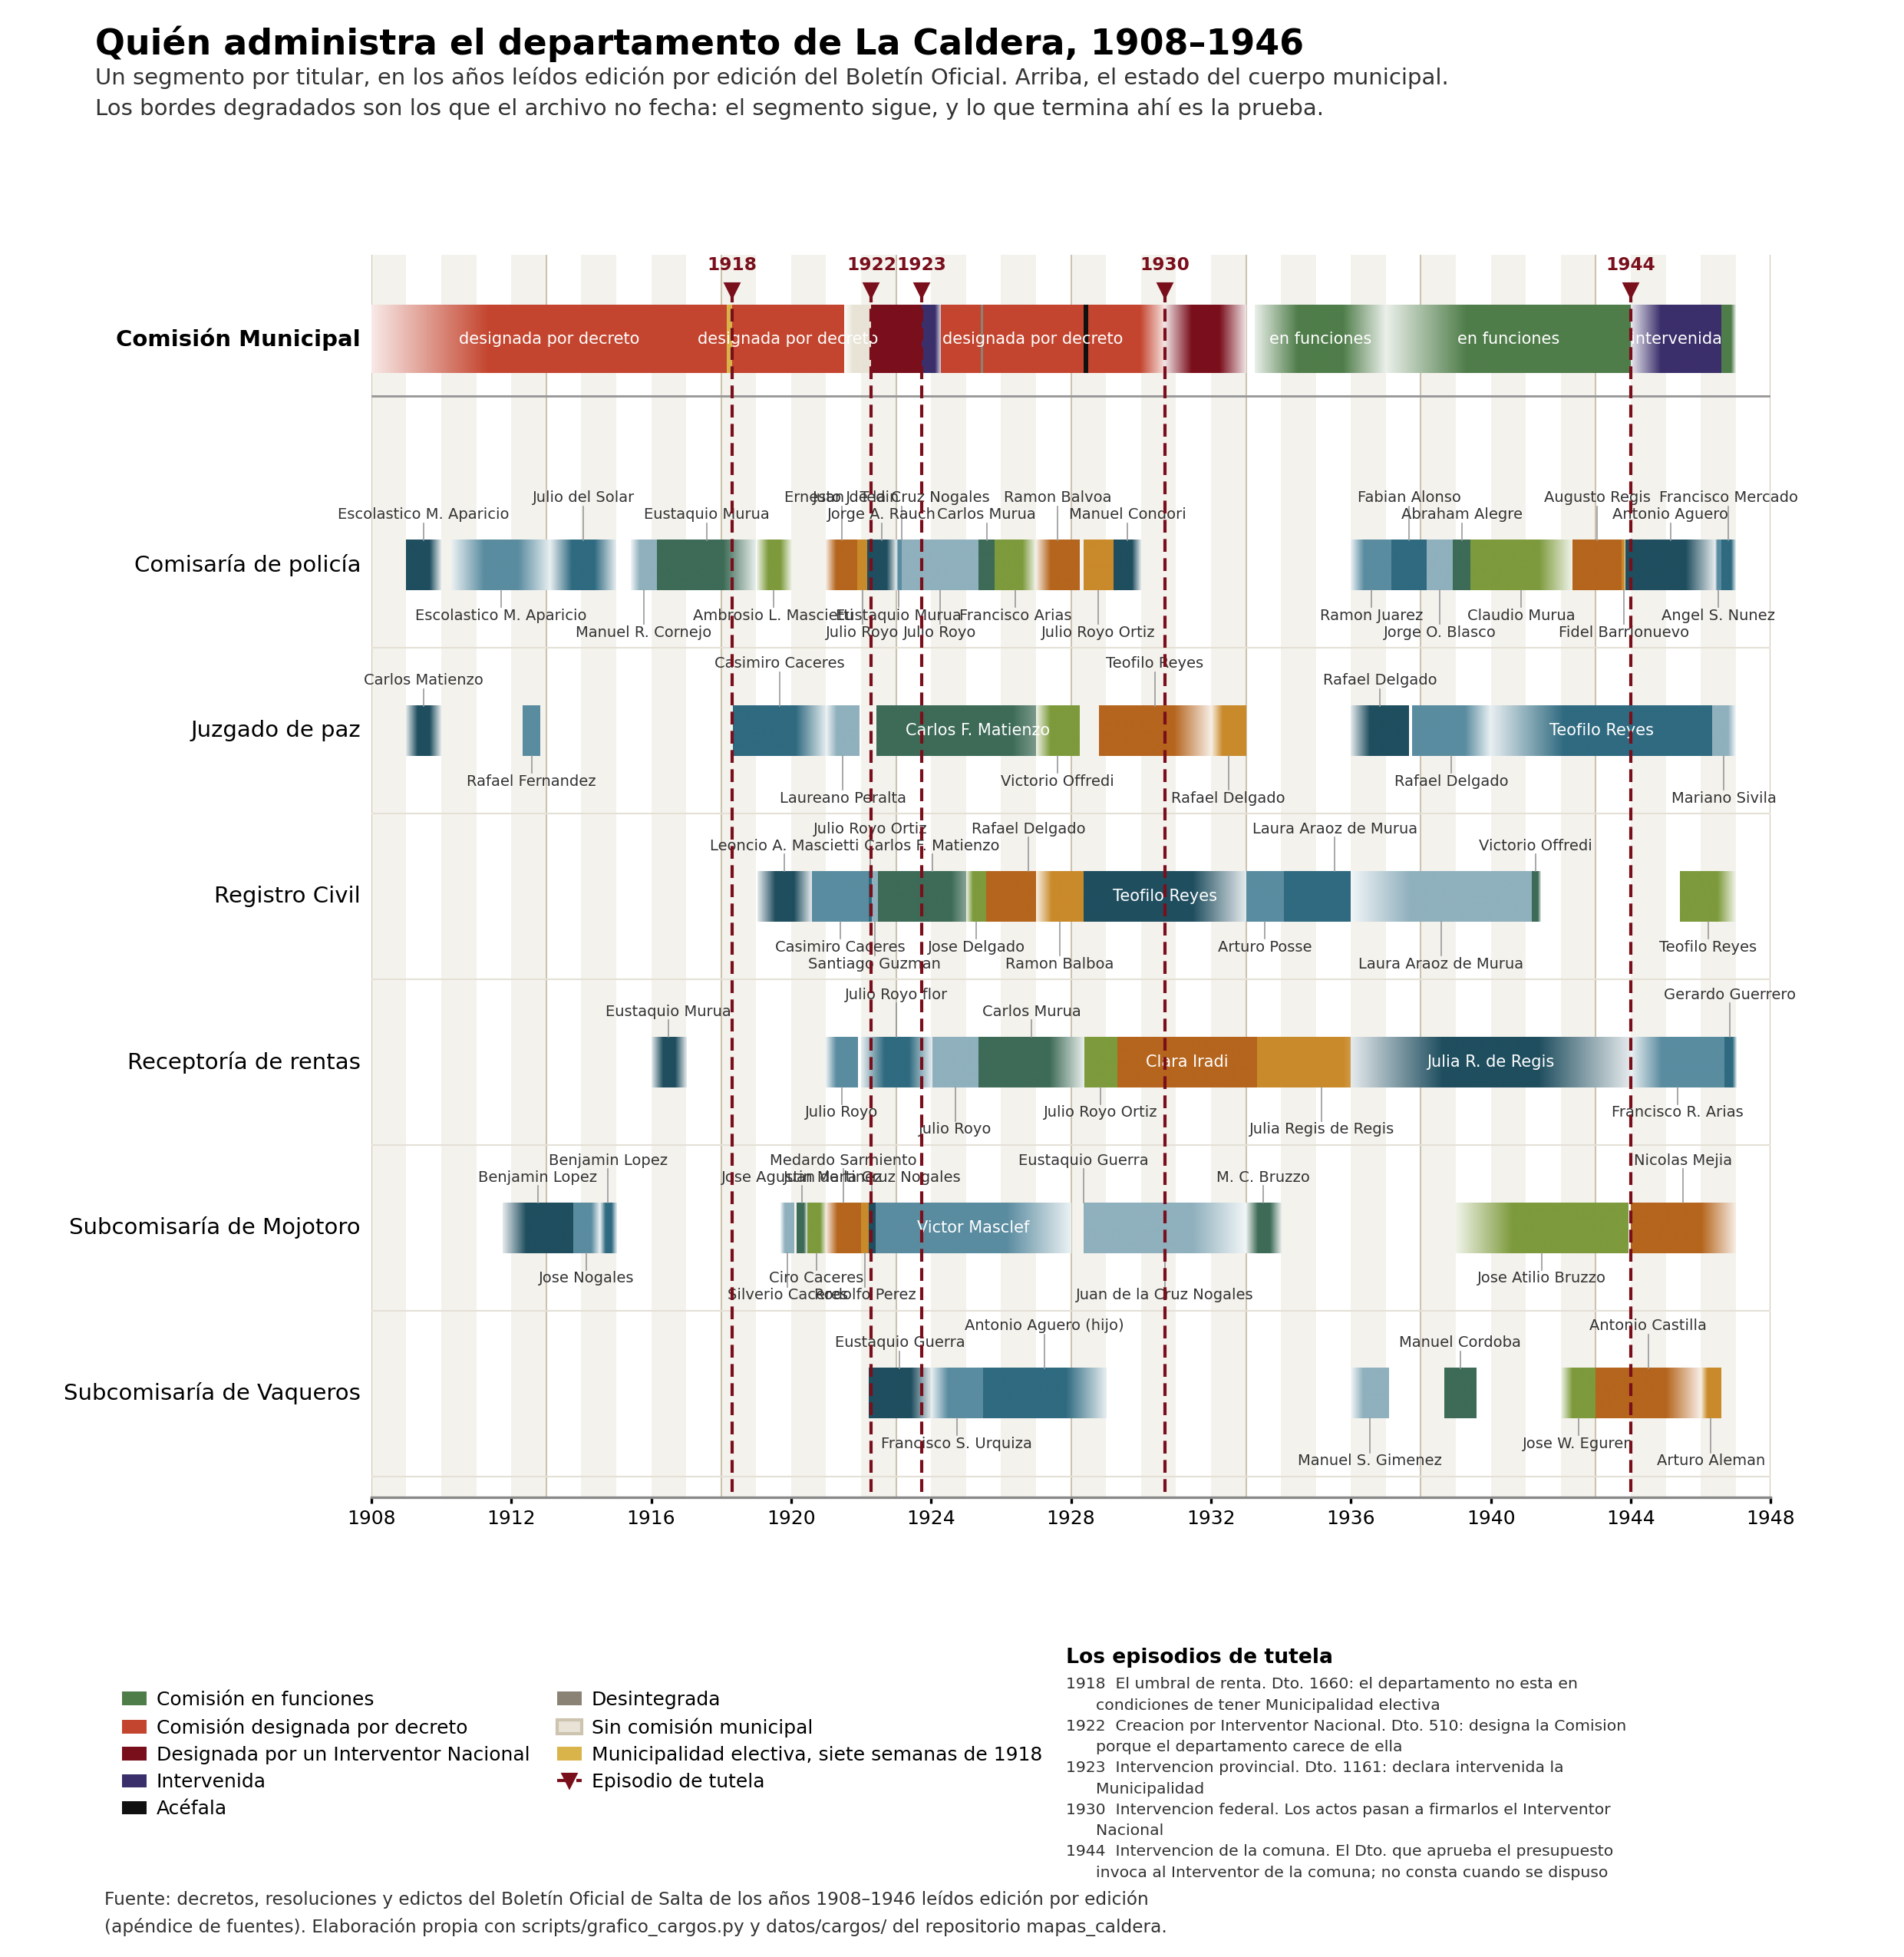
\includegraphics[width=\textwidth,height=0.88\textheight,keepaspectratio]{fig-cargos-linea.png}
\caption[Quién administra el departamento de La Caldera, 1908--1946]{\textbf{Quién administra el
departamento de La Caldera, 1908--1946.} Un segmento por titular en los seis cargos unipersonales
que el Boletín publica ---comisaría de policía, juzgado de paz, Registro Civil, receptoría de
rentas y las subcomisarías de Mojotoro y de Vaqueros---; arriba, separado, el estado de la
Comisión Municipal, que no es un cargo de una persona sino un cuerpo; y en línea vertical, los
cinco episodios de tutela. \textbf{Los bordes degradados son los que el archivo no fecha}: el
segmento sigue, y lo que termina ahí es la prueba ---cincuenta y ocho de los noventa y cuatro
bordes salen de un acto publicado, el cincuenta y nueve por ciento---. Todo sale de los años leídos
edición por edición (apéndice \ref{cap:fuentes}). Elaboración propia; dibujo de
\texttt{scripts/grafico\_cargos.py} sobre \texttt{datos/cargos/} del repositorio
\texttt{mapas\_caldera} (apéndice \ref{cap:fuentes}).}
\label{fig:cargos}
\end{figure}

\begin{cautela}
\textbf{Cuatro cosas se leen ahí que ningún año suelto deja ver.}

\textbf{La primera: el primer tercio está casi vacío.} De 1908 a 1920 hay cuatro segmentos en
toda la lámina. \textbf{No es que el departamento no tuviera cargos}: es que el Boletín no
publicaba los nombramientos, y sobre esos trece años el archivo sólo entrega un juez de paz en
1909, otro en 1912, un tercero en 1918 y un receptor de rentas en 1916. \textbf{Lo que la lámina
mide en esa mitad no es el gobierno del departamento sino la publicidad de sus actos.}

\textbf{La segunda: 1922 y 1923 son un enjambre.} La comisaría tiene cinco titulares entre
noviembre de 1921 y marzo de 1923; el Registro Civil, cuatro entre marzo y junio de 1922. Los
rótulos de esos segmentos no entran dentro de sus barras y hubo que escalonarlos en cuatro
alturas: \textbf{la ilegibilidad del dibujo en ese tramo es el dato}.

\textbf{La tercera: 1928 es un corte vertical.} Entre marzo y junio se cortan la comisaría, el
juzgado de paz, el Registro Civil, la receptoría y la subcomisaría de Mojotoro, y la Comisión
Municipal pasa por acefalía. \textbf{Ningún segmento cruza ese año entero.}

\textbf{Y una quinta, que el tramo 1937--1946 agrega.} La lámina llega ahora hasta 1946 y
muestra \textbf{el bloque más largo de toda la serie}: Augusto Regis\index{Regis, Augusto}
presidiendo la Comisión Municipal sin interrupción de 1937 a 1943, con su propio segmento
además en la fila de la comisaría en 1942 y 1943. \textbf{Y termina con la tercera
intervención}, que corre de 1944 a agosto de 1946 y cuyo borde izquierdo se degrada porque el
archivo no dice cuándo empezó.

\textbf{Y la cuarta: el caso de Urquiza\index{Urquiza, Francisco S.} ocupa dos filas a la vez}
---la subcomisaría de Vaqueros y, arriba, el cuerpo municipal--- en los mismos meses de 1924 en
que recibe la concesión de agua. \textbf{Y su segmento de la subcomisaría se degrada hacia la
izquierda}, porque el acto que lo nombró no aparece en ninguno de los tramos leídos: la lámina
dibuja esa ignorancia en lugar de taparla.
\end{cautela}

\begin{cautela}
\textbf{Qué no prueba la lámina \ref{fig:cargos}.} No prueba que un cargo estuviera vacante donde
no hay segmento: prueba que el Boletín no publicó quién lo ocupaba. No prueba la fecha exacta de
ningún relevo cuyo borde esté degradado. \textbf{Y mezcla, en la fila del juzgado de paz,
propietarios y suplentes}, porque varios actos no distinguen; el apéndice \ref{cap:personas} sí
los separa cuando el acto lo dice. La tabla que la produce ---\texttt{datos/cargos/}--- trae por
cada segmento el acto y la edición de donde sale, de modo que cualquiera puede ir a discutir
segmento por segmento.
\end{cautela}

\section{1937 y 1938: la primera defensa del río, y la renta escolar}

Los dos años se leyeron edición por edición y son los tramos vigésimo tercero y
vigésimo cuarto: las ediciones \textbf{1669 a 1721} y \textbf{1722 a 1773}. Es
el primer tramo del libro leído con una novedad material: \textbf{los PDF de
esta época ya traen capa de texto del proveedor}, de modo que el noventa y
nueve por ciento de las hojas no necesitó reconocimiento propio (apéndice
\ref{cap:fuentes}).

\begin{ficha}{Decreto de 1938 --- defensa sobre la margen izquierda del río La Caldera (B.O.\ Nº 1724, h.\ 19)}
Vecinos del departamento solicitan «\textit{la construcción de defensas sobre la
margen izquierda del río Caldera}», y el decreto recoge su fundamento:
«\textit{todos los años en la época de lluvias, las aguas del río Caldera
amenazan las propiedades con inminente peligro de perjuicio para los
cultivos}».

De los cómputos métricos, presupuestos y croquis de la obra «\textbf{defensa río
Caldera}», \textbf{proyectada en una longitud de cincuenta metros}, resulta su
costo.
\end{ficha}

\begin{cautela}
\textbf{Es el antecedente más antiguo de la defensa del río que este libro
persigue, y está ochenta años antes del amparo.} El capítulo
\ref{cap:amparo} cuenta que el Plan de Manejo de 2024 cifra la defensa del río
La Caldera en el cincuenta y ocho por ciento de toda su inversión, y que el
aluvión que lo motivó es de diciembre de 2018. \textbf{En 1938 los vecinos ya
pedían lo mismo, con el mismo argumento} ---que todos los años, en la época de
lluvias, el río amenaza las propiedades--- y el Estado provincial lo proyectó.

\textbf{Y la escala es la que hay que mirar.} Aquella obra tenía
\textbf{cincuenta metros}. La del Plan de 2024 se mide en kilómetros y en miles
de millones de pesos. \textbf{Ochenta y seis años entre el primer pedido
documentado y el primer plan cifrado.}

\textbf{Y el barrido de 1940 contesta qué pasó con aquellos cincuenta metros: no
se hicieron.} El decreto del Nº 1833, h.\ 46, pedido «\textit{con carácter de
urgencia}», lo dice entero: «\textit{el año ppdo.\ debieron efectuarse las obras
de defensa en el río de la Caldera, \textbf{las que fueron suspendidas en virtud
de que el mencionado río desvió su curso}}»; y agrega que «\textit{hoy
nuevamente amenazan peligro las aguas de este río \textbf{para la población de la
Calderilla}}». Lo que autoriza es «\textit{la construcción de un \textbf{reparo
provisorio} para defensa en el río de la Caldera en el lugar denominado la
Calderilla}».

\textbf{Tres cosas quedan establecidas, y las tres importan.} La primera: entre
1938 y 1940 hay \textbf{dos intentos de defender el río y ninguna obra
terminada}. La segunda: \textbf{el motivo de la suspensión es el propio río}
---desvió su curso--- y no la falta de fondos ni la desidia, que es el
argumento que un lector supondría. Y la tercera: \textbf{el peligro se corrió de
lugar}, de la margen izquierda en general a \textbf{la población de la
Calderilla} en particular.

\textbf{Eso es exactamente lo que el capítulo \ref{cap:amparo} discute ochenta
años después}, y con el mismo vocabulario: obras que se proyectan, un río que
cambia de curso, y defensas que se ejecutan como reparo provisorio. \textbf{Y el
archivo no registra que el reparo de 1940 se haya hecho tampoco.}

\textbf{Y el croquis, otra vez, se cita y no se publica.} El decreto lo nombra
entre las piezas que fundan el costo, como el de la acequia de Urquiza en 1923 y
como el plano de Hessling en 1911.
\end{cautela}

\subsection*{Y el municipio no pagaba la renta escolar}

\begin{ficha}{Decretos de 1938 sobre el balance municipal de 1937 (B.O.\ Nº 1750 h.\ 12 y Nº 1763 h.\ 6)}
La Comisión Municipal del distrito de La Caldera eleva el balance del ejercicio
1937. El Consejo de Educación informa que esa Comisión «\textit{no ha efectuado
ingreso alguno de contribución al fondo propio de educación}», y el Poder
Ejecutivo \textbf{devuelve el balance con observaciones}.

Un mes más tarde, con nuevo informe de la Comisión, el decreto del expediente
1117 M \textbf{aprueba el ejercicio 1937 y, de acuerdo al monto de los ingresos
habidos, deja establecido el porcentaje} que corresponde a ese fondo.
\end{ficha}

\begin{cautela}
\textbf{Cierra un hilo que este capítulo abrió en 1927 y dejó suelto.} El
decreto 5024 de aquel año aprobó la primera rendición de cuentas del municipio
«\textit{atento el informe del Consejo General de Educación que manifiesta su
conformidad en lo que respecta a la renta escolar que por dicho ejercicio le
corresponde}». Once años después, el mismo Consejo informa lo contrario: que el
municipio \textbf{no aportó nada}.

\textbf{De modo que la renta escolar no era una formalidad: era una
obligación que se controlaba, y que este municipio incumplió.} Y la Provincia
no la ejecuta ni la sanciona: devuelve el balance, pide informe y después fija
el porcentaje sobre lo efectivamente recaudado. \textbf{Sigue sin publicarse
una sola cifra}: ni el balance, ni el monto de los ingresos, ni el porcentaje.
Son el sexto y el séptimo acto económico del municipio publicados sin su
número.

\textbf{Y hay un renglón de 1938 que conviene transcribir aunque no nombre al
departamento en su parte dispositiva} (Nº 1738, h.\ 6): al discutir el
cumplimiento de las comunas de campaña, el acto dice que no lo ha hecho
«\textit{ninguna de las municipalidades de la campaña, a excepción de la de La
Caldera, que ocasionalmente lo ha hecho}». \textbf{Es la única vez en todo el
archivo temprano en que este departamento aparece como la excepción que
cumple}, y aparece en el mismo año en que el Consejo de Educación le observa el
balance por no aportar. Este libro transcribe las dos cosas y no las concilia.
\end{cautela}

\begin{cautela}
\textbf{Y tres piezas más de los dos años, que el apéndice
\ref{cap:cronologia} detalla.}

\textbf{«La Helvecia» era «la Calderilla».} El edicto de deslinde, mensura y
amojonamiento de 1937 (Nº 1691, h.\ 41) individualiza el inmueble
«\textit{denominada «la Helvecia» antes «Calderilla»}», con lindero norte en la
propiedad de \textbf{Augusto Regis}\index{Regis, Augusto} ---presidente de la
Comisión Municipal del departamento en ese mismo año---, al naciente los
herederos de \textbf{Pedro Valencia} y al poniente el \textbf{río de La
Caldera}. \textbf{Los dos nombres están en la lámina \ref{fig:parajesnom} como
topónimos distintos}, y este edicto dice que son el mismo lugar en dos momentos:
la nómina de 1938 los sigue imprimiendo separados, en el mismo circuito.

\textbf{El pueblo tuvo teléfono antes que agua de red.} El decreto de 1937
(Nº 1711, h.\ 5) paga «\textit{las reparaciones de las líneas telefónicas del
pueblo de La Caldera}», con los trabajos a cargo de \textbf{Rafael Delgado},
que ese mismo año es juez de paz propietario del distrito. \textbf{Reparar
supone que existían}, y el archivo no registra cuándo se instalaron.

\textbf{Y la nómina de 1938 resulta ser la de 1940, nombre por nombre.} El
departamento es el \textbf{Colegio Electoral Nº 2}, con los circuitos 5 y 6: la
mesa 1 vota en la Escuela Elemental Mixta con nueve parajes, la mesa 2 en la
Iglesia Parroquial con treinta y uno, y la del circuito 6 en la Escuela
Infantil Provincial de Vaqueros con siete. \textbf{Cuarenta y siete renglones y
cuarenta y seis nombres distintos} ---«Calderilla» se imprime dos veces, en las
mesas 1 y 2---, y \textbf{son exactamente los cuarenta y seis del padrón de
1940}: las cuatro diferencias del cotejo son variantes de grafía del mismo
lugar, «Corral de Barranca» por Barrancas, «Monte de las Garrapatas» por
Monte, «Potrero de Castilla» por Castillo y «Pueblo» por Pueblo (La Caldera).

\textbf{Eso corrige la lectura de la lámina en un punto que importa.} Catorce
nombres ---Helvecia, Getsemaní, Abra de la Sierra, Cañada Ancha, Severino,
Villa Urquiza, Santa Gertrudis, Entre Ríos, Mosquera, Nogalito, Los Matos,
Higueritas, Los Chusos y La Sierra--- figuraban como si aparecieran en 1940 por
primera vez. \textbf{Están en 1938 y son los mismos}, de modo que lo que la
lámina muestra en su última columna no es una ampliación de 1940 sino
\textbf{una lista que ya estaba armada dos años antes y no se tocó}. Y uno de
esos nombres tiene explicación en el mismo año: «La Helvecia» es el nombre
nuevo de «la Calderilla», y las dos figuran en el mismo circuito.

\textbf{Y la segunda concesión de agua del departamento se pide en 1938 y se
resuelve en 1939.} Un particular ---Isaac Fernández--- solicita «\textit{la
concesión de agua}» para regadío de la finca \textbf{«Campo Alegre»}, con título
inscripto «\textit{al folio 374, asiento 475 del libro D de títulos de la
Caldera}», y el trámite corre «\textit{con intervención del señor Fiscal de
Gobierno y de la Municipalidad de la Caldera}» (Nº 1746, h.\ 27 y 28).
\textbf{Catorce años después de la de Urquiza, el mecanismo es idéntico}: la
solicita un propietario, informa el municipio, dictamina el fiscal.

\textbf{Y el acto que lo resuelve, en 1939, trae la pieza que este libro venía
buscando} (Nº 1796, h.\ 23): entre sus considerandos, la oposición al pedido
invoca «\textit{la existencia de una \textbf{ordenanza dictada por el municipio
de la Caldera en fecha octubre 13 de 1914}, que reglamenta la distribución de la
totalidad}» del caudal.

\textbf{Es la ordenanza de 1914 que el capítulo \ref{cap:infraestructura} usa
como prueba de que el municipio decidía sobre el agua de su suelo, y acá aparece
citada veinticinco años después como derecho vigente}, en un expediente
provincial, y esgrimida contra una concesión nueva. \textbf{No es sólo que la
ordenanza existió: es que todavía se invocaba}, y que la Provincia tuvo que
pronunciarse sobre ella. Lo que el archivo no dice es cómo resolvió.

\textbf{Y reaparece el apellido Quipildor, ahora como sucesión y con
superficie.} Un pedimento minero de \textbf{dos mil hectáreas (cuatro unidades)}
se ubica sobre las fincas \textbf{Rosal y Potrero, «propiedad de la sucesión
Quipildor»}, en los departamentos de Rosario de Lerma y Caldera (Nº 1726 h.\ 40
y Nº 1730 h.\ 45). \textbf{Es el mismo apellido que en 1925 aparecía como dueño
de los terrenos donde Larrán pidió su cateo}, y trece años después sigue siendo
propietario en el departamento ---ahora como sucesión, y con dos fincas
nombradas---. Coincidencia de nombre, como siempre.

\subsection*{Y en 1940 el departamento entra en la red vial de la provincia}

El decreto que fija la red vial provincial de 1940 incorpora dos trazas que
pasan por el departamento (Nº 1875, h.\ 21): «\textit{de la Calderilla a río
Saladillo por Gallinato y Campo Santo}», y una ruta que corre «\textit{por el
Jardín, Pampa Grande, Guachipas, La Viña, Cerrillos, Salta, \textbf{Vaqueros,
Calderilla, hasta Tres Cruces en el límite con Jujuy}}».

\begin{cautela}
\textbf{Esa segunda traza es la que hoy se llama Ruta Nacional 9}, y el
decreto la describe atravesando el departamento de sur a norte, por Vaqueros y
la Calderilla, hasta el límite provincial. \textbf{Es la primera vez que el
archivo temprano ubica al departamento dentro de una red y no como punto
aislado}: hasta 1939 los caminos que lo nombran son tramos ---Calderilla al
Desmonte, Calderilla a Campo Santo, Calderilla al río Las Pavas--- y en 1940 es
un pasaje.

\textbf{El capítulo \ref{cap:infraestructura} lee ese pasaje noventa años
después como la forma del problema}: un territorio que la ciudad atraviesa. El
decreto de 1940 lo escribe sin ninguna intención de decirlo.
\end{cautela}

\subsection*{Y Regis es, a la vez, presidente del municipio y diputado provincial}

\begin{cautela}
\textbf{Es la décima superposición de la serie y la más directa de todas.} En
1940, al pedir ciento cincuenta pesos de ayuda para la comisión pro-fiestas
patronales del pueblo, el Boletín identifica al solicitante como
«\textit{el señor presidente de la comisión municipal del distrito de la
Caldera, \textbf{diputado provincial don Augusto Regis}}»\index{Regis, Augusto}
(Nº 1875, h.\ 2).

\textbf{No es un cargo que coincide con otro dentro del departamento ni un
propietario que legisla: es la misma persona presidiendo el municipio y
sentada en la Legislatura que lo regula.} Y no es un año: Regis preside la
Comisión Municipal \textbf{sin interrupción desde 1937}, reelecto por decreto en
1937, 1938, 1939 y 1940 ---cuatro «nuevos períodos legales de funciones»
seguidos---, y es el mismo hombre que el Interventor Nacional nombró a ese
cuerpo en abril de 1922 y que renunció dos veces, en 1922 y en 1923.
\textbf{Dieciocho años en el mismo cuerpo, con dos salidas en el medio}, y al
final presidiéndolo desde una banca.
\end{cautela}

\begin{cautela}
\textbf{Y cuatro cosas más que los dos años dejan, y que el apéndice
\ref{cap:cronologia} detalla.}

\textbf{El cuerpo municipal cambia de nombre.} En 1940 el Boletín ya no habla
de miembros de la Comisión Municipal sino de \textbf{concejales titulares y
suplentes}: por La Caldera, Eugenio Muñoz y José Manuel Alfaro. \textbf{Es la
primera vez en treinta y dos años de archivo} que el cuerpo del departamento se
nombra así.

\textbf{Dos escuelas nacionales más.} La Ley 4874 ---la ley Láinez--- instala
escuela en \textbf{San Alejo} en 1939 y en \textbf{Gallinato} en 1940, después
de la de San Alejo de 1924. \textbf{El Estado nacional pone tres escuelas en el
departamento entre 1924 y 1940}, y la Provincia se limita a consentir cada vez.

\textbf{Un apellido andino preside, por fin, del lado de la mesa.} En la mesa 1
del circuito 5 de 1940 es suplente primero \textbf{Severino Mamani}: es
\textbf{el primer apellido de origen andino que el archivo registra como
autoridad de mesa} del departamento, y Mamani es uno de los seis que el revalúo
de 1944 traerá entre sus titulares.

\textbf{Y un comisario destituido con causa escrita.} En 1939 una información
sumaria comprueba contra \textbf{Abraham Alegre}, comisario de policía de La
Caldera, «\textit{actos graves de inconducta y comisión de hechos}» que el acto
enumera, y lo separa del cargo «\textit{sin perjuicio de las acciones
judiciales a que hubiere lugar}»; lo reemplaza \textbf{Claudio Murúa}. \textbf{De
los más de setenta relevos que este capítulo registra entre 1908 y 1946 ---la
lámina \ref{fig:cargos} los cuenta---, es el único que dice la causa con esas palabras}: los demás usan la fórmula o callan.
\end{cautela}

\textbf{Y las autoridades del bienio se renuevan enteras otra vez.} La
comisaría pasa por \textbf{Ramón Juárez} ---que pide licencia en enero de 1937 y
renuncia en marzo---, \textbf{Fabián Alonso} interino, \textbf{Jorge O.\ Blasco}
y, al cierre de 1938, \textbf{Abraham Alegre}, permutado con el comisario de
San Carlos. La subcomisaría de Vaqueros cambia cuatro veces. Y la elección de
1938 da por el departamento al senador \textbf{Florentino M.\ Serrey}
\index{Serrey, Carlos} por un partido y a \textbf{Francisco Mercado} con
\textbf{Teófilo Reyes} de suplente por el otro, y compone la Comisión Municipal
con \textbf{Eustaquio Murúa}\index{Murúa, Eustaquio} y Eugenio Muñoz como
titulares y \textbf{Genaro Molina} entre los suplentes. \textbf{Murúa y Molina
llevan entonces veintidós y veintinueve años apareciendo en este archivo}, y
Serrey es el apellido que en 1923 era dueño de la finca Vaqueros y que en 1985
todavía figura en la expropiación de la Ley 6334 (capítulo
\ref{cap:expropiacion}).

\textbf{Y los caminos se pagan quincena por quincena.} Los dos años traen
decenas de órdenes de pago de Vialidad por los caminos \textbf{Calderilla--El
Desmonte por Gallinato}, \textbf{Calderilla--Campo Santo} y
\textbf{Calderilla--Güemes por Gallinato}: jornales de cuadrilla, ripio de
Jorge Cornejo, liquidaciones al contratista Adolfo Martínez, capataces con
nombre y apellido. \textbf{Es el primer tramo del archivo en que una obra del
departamento se puede seguir semana a semana}, y queda como serie a reconstruir.
\end{cautela}

\section{1941: un agente muerto en la Calderilla, y tierra que se compra para un camino}

El año se leyó edición por edición y es el vigésimo séptimo tramo: las ediciones
\textbf{1878 a 1929}. Deja, además del cierre de la mina, dos actos que el libro
no tenía.

\begin{ficha}{Expediente de pensión --- B.O.\ Nº 1907, h.\ 5 (1941)}
La viuda de \textbf{don Paulino Fernández}, «\textit{extinto agente de policía de
la comisaría de la Caldera}», pide ser acogida a los beneficios de la ley, y
acredita el vínculo «\textit{en mérito de los testimonios expedidos por la
oficina del registro civil de la Caldera}».

El informe del expediente dice que el causante murió «\textit{[en el] punto
denominado “la Calderilla” de resultas de un tiro de revólver que le
descerrajara \textbf{Abel Murúa}}».
\end{ficha}

\begin{cautela}
\textbf{Es la primera muerte violenta que el archivo temprano registra en el
departamento}, y llega por la vía menos previsible: un trámite de pensión.

\textbf{Lo que el libro afirma es lo que el acto dice, y nada más}: que el
Estado provincial, al resolver una pensión, consignó esa causa de muerte con
ese nombre. \textbf{No es una condena ni consta aquí su resultado judicial}: el
archivo leído no trae la causa penal, y este libro no la busca ni la supone. El
apéndice \ref{cap:pedidos} la reclama, porque es lo único que permitiría decir
algo más.

\textbf{Y el apellido vuelve.} Murúa recorre este capítulo desde 1912 ---jurado
de patentes, comisario del departamento en 1916, 1923, 1930 y 1932, causante del
sucesorio que remata La Calderilla en 1923, titular de La Despensa en 1925,
miembro de la Comisión Municipal en 1938 y comisario otra vez en 1939---.
\textbf{Coincidencia de nombre, como siempre, y en este caso con más razón que
nunca para no inferir nada.}
\end{cautela}

\begin{cautela}
\textbf{Y por primera vez el Estado compra tierra en el departamento para hacer
un camino.} El decreto del Nº 1880, h.\ 8, considera «\textit{imprescindible}»
la adquisición ---o venta--- de «\textit{los terrenos necesarios para la
ejecución de las mejoras del camino Calderilla a río de las Pavas, tramo
Desmonte-Campo Santo}», y encarga la gestión.

\textbf{Hasta 1940 los caminos del departamento aparecen como jornales, ripio y
certificados de obra: nunca como tierra.} Éste es el primer acto en que la traza
exige comprar el suelo por donde pasa, y cae sobre el mismo camino que desde
1937 concentra casi todo el gasto vial del departamento. \textbf{Quién era dueño
de esos terrenos y cuánto se pagó no se publica}, y el apéndice
\ref{cap:pedidos} lo pide: es el antecedente más antiguo de la relación entre
una traza y el dominio del suelo que este libro discute en el capítulo
\ref{cap:expropiacion} para 1985.

\textbf{Y un apellido andino al frente de una cuadrilla.} El mismo año autoriza
la permanencia en obra de la cuadrilla «\textit{a cargo del peón de 1.ª don
\textbf{Manuel Apaza}}». Apaza es otro de los seis apellidos del revalúo de 1944,
y aquí aparece dirigiendo trabajo en el camino.
\end{cautela}

\section{1942 y 1943: la concesión de 1885 aparece entera}

Los dos años se leyeron edición por edición y son los tramos vigésimo octavo y
vigésimo noveno: las ediciones \textbf{1930 a 1982} y \textbf{1983 a 2035}.

\begin{ficha}{Inscripción de derechos de agua --- B.O.\ Nº 1948, h.\ 24 (1942)}
Del registro inmobiliario consta que «\textit{por \textbf{acuerdo de la
Municipalidad de la Caldera de fecha 4 de junio de 1885}, se concedió a don
\textbf{Eustaquio Murúa}}»\index{Murúa, Eustaquio} el uso de \textbf{treinta
litros de agua por segundo del río Wierna}, y que a la finca «\textit{denominada
\textbf{Sausal o Curuzú}, ubicada en el distrito de Vaqueros, departamento de la
Caldera}» le corresponde ese uso por ser su titular sucesor «\textit{en la
posesión}» de los anteriores propietarios.
\end{ficha}

\begin{cautela}
\textbf{El capítulo \ref{cap:planteo} situaba el punto de partida de la voz
municipal sobre el agua en 1885 y no tenía el acto.} Ahora está: \textbf{la
fecha exacta ---4 de junio de 1885---, el beneficiario, el caudal y la finca}.

\textbf{Y el beneficiario es un Murúa}, cincuenta y siete años antes de que el
apellido recorra este capítulo como comisario, jurado de patentes, causante de
sucesorio y titular de La Despensa. \textbf{Es la aparición más antigua de ese
apellido en el departamento} que este libro registra, y llega por un acto del
municipio concediéndole agua.

\textbf{Y hay una segunda, del mismo año, que dice algo distinto} (Nº 1964,
h.\ 22): sobre el \textbf{río de las Nieves, naciente del Wierna}, se reconocen
derechos «\textit{otorgado[s] por la Municipalidad de la Caldera}» y
«\textit{reconocidos como tales \textbf{desde fecha inmemorial}}», para la finca
«Yacones» o «Tránsito». \textbf{«Desde fecha inmemorial» es una fórmula, no una
fecha}, y este libro no la convierte en una: registra que en 1942 la Provincia
inscribió como propios derechos que el municipio había otorgado sin que conste
cuándo.

\textbf{Las dos inscripciones son del mismo año en que el capítulo
\ref{cap:infraestructura} sitúa la pérdida de esa voz.} Y ahora se entiende
mejor por qué: \textbf{1942 es el año en que los derechos que el municipio había
concedido pasan a los registros provinciales}. No se los quitaron: se los
anotaron a nombre de otro registro.
\end{cautela}

\subsection*{Y Regis es, además, comisario de policía}

\begin{cautela}
\textbf{Es la undécima superposición y la que completa el cuadro.} El decreto
del Nº 1952, h.\ 16, de 1942, «\textit{nombra comisario de policía de la
Caldera, con anterioridad al día 1.º del mes en curso, al señor \textbf{Augusto
Regis}}»\index{Regis, Augusto}. En 1943 se le liquidan haberes «\textit{como
comisario de policía de la localidad de la Caldera, durante nueve días del mes
de setiembre}», y después \textbf{renuncia} al cargo (Nº 2021, h.\ 14).

\textbf{En el mismo bienio es reelecto presidente de la Comisión Municipal}, por
decreto, en 1942 y en 1943 ---sexto y séptimo «nuevo período legal de
funciones» consecutivos---. De modo que Augusto Regis es, a la vez y en actos
publicados: \textbf{presidente del cuerpo que gobierna el departamento,
diputado provincial y comisario de policía del mismo departamento}.

\textbf{No hace falta inferir nada.} Este capítulo viene registrando desde 1909
que el que manda la policía integra el cuerpo municipal ---Aparicio\index{Aparicio, Escolástico M.}
en 1910, Rauch en 1922---. \textbf{En 1942 las dos cosas son la misma persona y
además legisla.} Es el punto más alto de una serie de treinta y tres años, y el
archivo lo publica sin comentario.
\end{cautela}

\begin{cautela}
\textbf{Y en 1943 la Provincia regulariza por prescripción el terreno de su
propia comisaría.} Un edicto anuncia «\textit{juicio de posesión treintañal de un
inmueble ubicado en el pueblo de la Caldera, donde se encuentra emplazado el
edificio ocupado por la \textbf{comisaría de policía}}», \textbf{deducido por el
Gobierno de la Provincia de Salta}, con cuarenta metros de frente por doscientos
de fondo, lindando al oeste con «\textit{la calle principal del pueblo}» y con
\textbf{Daniel Linares}\index{Linares, Daniel}; y el auto ordena oficiar
«\textit{a la Municipalidad de la Caldera para que informe si afecta propiedad
municipal}» (Nº 1994, h.\ 48, y Nº 2001, h.\ 22).

\textbf{Treinta años de posesión quiere decir que el Estado ocupaba ese terreno
desde 1913 o antes, sin título.} Y quien tiene que informar si le pertenece es
el municipio, que en ese momento preside el hombre que acababa de ser comisario
en ese mismo edificio. \textbf{El archivo no dice cómo terminó}, y el apéndice
\ref{cap:pedidos} lo pide.
\end{cautela}

\section{1944: el revalúo en su sitio, y otra comuna intervenida}

El año se leyó edición por edición y es el trigésimo tramo. Trae dos cosas que
corrigen la lectura de piezas que el libro ya usaba.

\begin{cautela}
\textbf{El revalúo de 1944 no es un padrón del departamento: es un padrón
provincial en el que el departamento ocupa un tramo.} El barrido lo ubica en el
Boletín \textbf{Nº 2166}, y el cuadro corre por lo menos de la hoja 6 a la 76,
con números de partida que pasan de los cinco mil. \textbf{El renglón
«\textit{departamento de la Caldera}» abre una sección dentro de esa serie}
(h.\ 6).

\textbf{Eso confirma la cautela que el capítulo \ref{cap:fincas} ya traía} ---que
no se sabe si las cuarenta y siete partidas publicadas son todas las del
departamento o sólo las revaluadas--- \textbf{y la vuelve más precisa}: lo que
el Boletín publica es un revalúo general de la Provincia, y el tramo del
departamento es lo que cabe en su sección. \textbf{La pregunta ya no es si el
padrón está completo, sino qué criterio decidió qué partidas entraban}, y el
apéndice \ref{cap:pedidos} la pide así.

\textbf{Y un apellido del cuadro merece registrarse}: entre los titulares del
tramo departamental figura \textbf{«Caldera, Dominga M.\ de»}, con quinientos
pesos de valuación. \textbf{Es el nombre del departamento como apellido de una
titular}, y este libro no infiere nada de eso salvo que conviene no confundirlo
en una búsqueda.
\end{cautela}

\begin{ficha}{Decreto de 1944 sobre el presupuesto municipal (B.O.\ Nº 2053, h.\ 4)}
«\textit{Visto este expediente en el que el señor \textbf{Interventor de la
comuna de la Caldera} eleva a conocimiento y aprobación del Poder Ejecutivo el
proyecto de ordenanza}»: se aprueba «\textit{el cálculo de recursos y
presupuesto de gastos de la \textbf{Municipalidad de la Caldera}, para regir
durante el ejercicio económico 1944 en curso}», y se devuelve el expediente
6463-M.
\end{ficha}

\begin{cautela}
\textbf{Es la tercera intervención del cuerpo municipal que este capítulo
registra}, después de la provincial de 1923 y la federal de 1930, y la primera
en que el interventor aparece ejerciendo la función ordinaria: elevar el
presupuesto. \textbf{El decreto no dice cuándo se dispuso la intervención ni
quién es el interventor}, y ningún acto del año leído lo nombra: \textbf{el
archivo registra el efecto y no el acto}, que es el mismo mecanismo que el
capítulo \ref{cap:opacidad} describe.

\textbf{Y el cuerpo cambió de nombre otra vez.} En 1940 eran concejales, en 1942
y 1943 volvió a ser Comisión Municipal, y en 1944 el mismo decreto lo llama
\textbf{«comuna»} en el vistos y \textbf{«Municipalidad»} en el artículo.
\textbf{Cuatro nombres para el mismo cuerpo en cuatro años}, y este libro los
transcribe sin normalizar.
\end{cautela}

\begin{cautela}
\textbf{Y la comisaría del pueblo se refacciona el año siguiente al juicio por
su terreno.} En 1943 la Provincia promovió posesión treintañal del inmueble
«\textit{donde se encuentra emplazado el edificio ocupado por la comisaría de
policía}»; en 1944 se licitan y ejecutan las obras de refección de ese local,
con presupuesto de \textbf{\$4.363,50}, contratista \textbf{Francisco Crescini} y
certificado final de \textbf{\$5.018,02}, más un adicional (Nº 2048 h.\ 48,
Nº 2053 h.\ 18, Nº 2094 h.\ 6 y Nº 2112 h.\ 7).

\textbf{Primero el título, después la obra}, y en ese orden. Es la primera vez
en treinta y seis años de archivo que el departamento tiene una obra pública
propia seguida paso a paso ---licitación, adjudicación, certificado, adicional
y devolución del depósito en garantía--- \textbf{y no es una escuela, ni un
camino, ni una defensa del río: es la comisaría}.
\end{cautela}

\section{1945: la defensa del río, tercer intento}

El año se leyó edición por edición y es el trigésimo primer tramo. Su hallazgo
cierra un hilo que este capítulo viene siguiendo desde 1938.

\begin{ficha}{Las obras de defensa en el río de la Caldera, 1945}
\textbf{Julio:} la Dirección General de Hidráulica llama a \textbf{licitación
pública} para «\textit{las obras de defensa a efectuarse en el río de la
Caldera}», con presupuesto de \textbf{\$2.515} y sobre el expediente 18385. El
aviso se repite en dieciséis ediciones seguidas.

\textbf{3 de septiembre:} el decreto 8549 autoriza la ejecución.

\textbf{Noviembre:} un decreto resuelve «\textit{ejecutar \textbf{por vía
administrativa} las obras de defensa en el río de la Caldera}» (Nº 2429,
h.\ 5).
\end{ficha}

\begin{cautela}
\textbf{Es el tercer intento en siete años, y el primero que llega a llamarse a
licitación.} En 1938 el proyecto era de cincuenta metros y quedó en croquis; en
1940 la obra «\textit{fue suspendida en virtud de que el mencionado río desvió
su curso}» y se autorizó un reparo provisorio; en 1945 hay presupuesto, llamado
público y expediente.

\textbf{Y termina como los otros dos: sin licitación.} «Por vía administrativa»
quiere decir que el Estado la hace por su cuenta, sin contratista, y el archivo
no publica después ni certificado ni recepción ---a diferencia de la refección
de la comisaría de 1944, que sí dejó licitación, adjudicación, certificado
final, adicional y devolución del depósito---. \textbf{Del edificio de la
comisaría queda el expediente completo; de la defensa del río, sólo la
autorización.}

\textbf{Y la escala cierra el argumento.} 1938: cincuenta metros. 1945:
\textbf{dos mil quinientos quince pesos}, cuando la refacción de la comisaría
del año anterior costó \textbf{cinco mil dieciocho}. \textbf{La defensa del río
valía la mitad que pintar y arreglar la comisaría}, y el capítulo
\ref{cap:amparo} cuenta que ochenta años después esa misma defensa se cifra en
el cincuenta y ocho por ciento de un plan de veintitrés mil millones.
\end{cautela}

\begin{cautela}
\textbf{Y dos actos de escuela que miden población.} El Consejo pide trasladar
la escuela Nº 250 de \textbf{Wierna} «\textit{por encontrarse despoblado dicho
lugar}», a «\textit{San Francisco, partido de Yacones}»; y aprueba instalar una
escuela nacional de la Ley 4874 en \textbf{San Alejo}, «\textit{lugar donde
según censo practicado existe una población de \textbf{51 niños} en edad
escolar}».

\textbf{Es el primer dato de población de un paraje del departamento que el
archivo temprano publica}, y no viene de un censo general sino de un trámite de
escuela: cincuenta y un chicos en San Alejo en 1945. \textbf{Y en el mismo año
Wierna se declara despoblado.} Los dos parajes están en las doce nóminas de la
lámina \ref{fig:parajesnom}; uno tiene escuela y el otro deja de tenerla.
\end{cautela}

\section{1946: el agua se reparte por zonas, y el municipio colabora}

El año se leyó edición por edición y es el trigésimo segundo tramo. Era el último de
esta ventana hasta que se incorporaron 1947 y 1948; \textbf{es el último leído con lectura sobre la imagen}, y en ese sentido cierra la serie verificada.

\begin{ficha}{Distribución de caudales del río Mojotoro (B.O.\ Nº 2686, h.\ 5 y 6)}
Considera «\textit{que el río Mojotoro forma su caudal con el proveniente de los
ríos \textbf{Wierna, la Caldera y Castellanos}}», y divide el sistema en zonas
para el estudio de la distribución: la \textbf{zona II} «\textit{abarca desde la
confluencia de los ríos \textbf{la Caldera y Vaqueros} hasta aguas arriba de la
primera toma del sistema}».

Dispone que \textbf{cuando el caudal de la zona I se mantenga inferior a
\textbf{2.500 litros por segundo}} se prohíban determinados usos, y su
\textbf{artículo 5º} establece que «\textit{las municipalidades de \textbf{Campo
Santo y de la Caldera} prestarán a la Dirección General de Hidráulica la
\textbf{colaboración necesaria}}».
\end{ficha}

\begin{cautela}
\textbf{Es el final del arco que este capítulo abrió en 1885, y lo dice en una
línea.} En 1885 la Municipalidad de La Caldera \textbf{concedía} treinta litros
por segundo del Wierna. En 1914 \textbf{reglamentaba} la distribución de la
totalidad del caudal por ordenanza. En 1929 una ley le dio a Campo Santo la
facultad de \textbf{vigilar y prohibir} bocas-tomas desde las juntas del Wierna.
En 1931 los dos municipios integraron una comisión \textit{ad hoc}. En 1942 los
derechos que el municipio había otorgado pasaron a los registros provinciales.
\textbf{Y en 1946 la Dirección General de Hidráulica fija zonas y umbrales, y a
los dos municipios les asigna «la colaboración necesaria».}

\textbf{Conceder, reglamentar, integrar una comisión, colaborar.} Sesenta y un
años, y el verbo cambia cuatro veces en la misma dirección. \textbf{Ninguno de
los actos deroga al anterior}: la facultad no se quita, se diluye.

\textbf{Y el umbral es la primera cifra hidrológica del departamento que el
archivo publica}: dos mil quinientos litros por segundo en la zona I. El
capítulo \ref{cap:ribera} trabaja con las series de aforo desde 1944; ésta es la
primera vez que un acto fija un número y le cuelga una prohibición.
\end{cautela}

\begin{cautela}
\textbf{Y el municipio publica un balance con cifras, por primera vez desde
1908.} El Boletín Nº 2473 trae el «\textit{Balance del movimiento de la renta}»
de la \textbf{comuna del departamento Caldera}, cuarto trimestre de 1945, con
sus renglones de entradas y salidas, sus saldos mensuales ---\$98,15 al cerrar
octubre, \$98,02 en noviembre--- y la firma de \textbf{F.\ Mercado} al pie de
cada mes.

\textbf{Rompe una serie de treinta y ocho años.} Entre 1922 y 1944 este capítulo
registró \textbf{siete actos económicos del municipio publicados sin una sola
cifra}: presupuestos aprobados por remisión al expediente, rendiciones
aprobadas sin transcribir, balances devueltos con observaciones. \textbf{En 1946
se publica el balance mismo}, y lo que muestra es un municipio que mueve
\textbf{menos de cien pesos por mes}.

\textbf{Y lo publica un interventor.} Francisco Mercado firma ese balance como
interventor de la comuna, y en abril de 1946 renuncia al cargo; el 6 de agosto
un decreto \textbf{da por terminada la intervención} a la Municipalidad de La
Caldera y designa presidente de la Comisión Municipal a Enrique Alejandro
Pfister. \textbf{La tercera intervención del cuerpo duró al menos tres años}
---estaba vigente en 1944 y el archivo no dice cuándo empezó--- y el único
balance con cifras de todo el período lo firma el interventor.
\end{cautela}

\begin{cautela}
\textbf{Y un falso positivo que conviene dejar escrito porque puede repetirse.}
En 1946 se autoriza instalar una escuela de la Ley 4874 «\textit{en la localidad
de \textbf{la Calderilla (departamento de la Capital)}}». \textbf{Hay una
Calderilla en el departamento Capital}, distinta de la de este departamento, y
el barrido la trae porque el término es el mismo. Este libro no la cuenta, y la
declara para que nadie la sume por descuido.
\end{cautela}

\section{1947: el municipio es el departamento entero}

\begin{figure}[p]
\centering
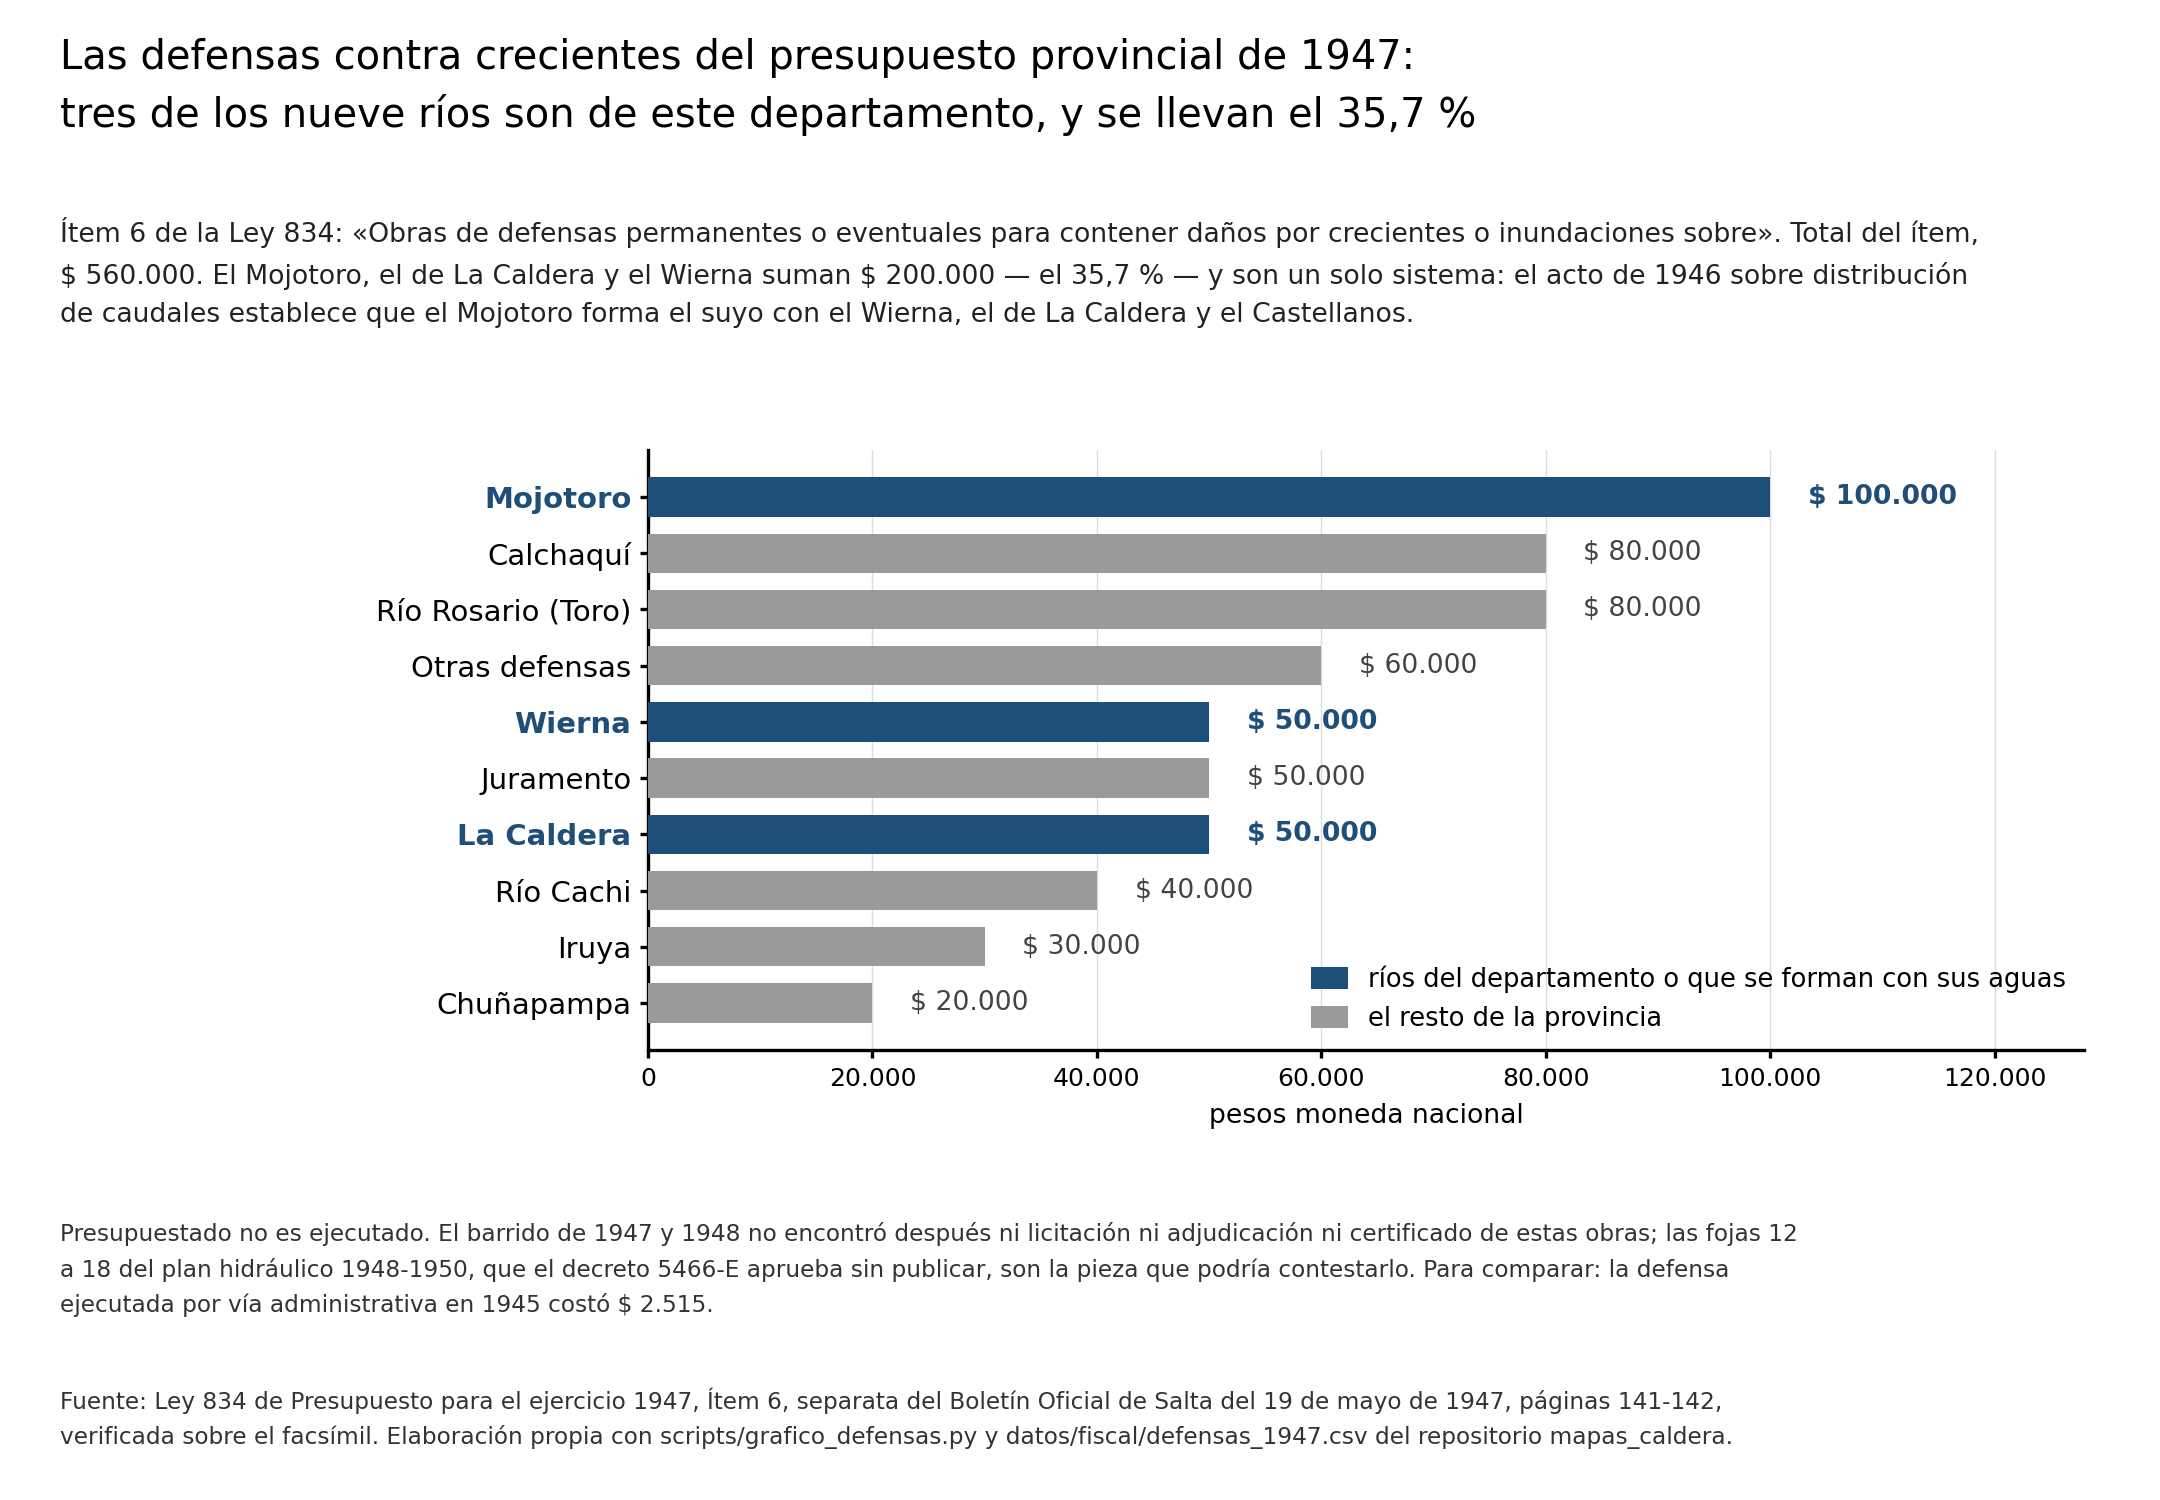
\includegraphics[width=\textwidth,height=0.88\textheight,keepaspectratio]{fig-defensas-1947.png}
\caption[Las defensas contra crecientes del presupuesto provincial de 1947]{\textbf{Las defensas
contra crecientes del presupuesto provincial de 1947: tres de los nueve ríos son de este
departamento, y se llevan el 35,7 por ciento.} El Ítem 6 de la Ley 834 ---«\textit{Obras de
defensas permanentes o eventuales para contener daños por crecientes o inundaciones sobre}»---
reparte \$560.000 entre nueve ríos y un renglón de imprevistos. \textbf{El Mojotoro, el de La
Caldera y el Wierna suman \$200.000}, y son un solo sistema: el acto de 1946 sobre distribución de
caudales establece que el Mojotoro forma el suyo con el Wierna, el de La Caldera y el Castellanos.
\textbf{Presupuestado no es ejecutado}: el barrido de 1947 y 1948 no encontró después ni licitación
ni adjudicación ni certificado de estas obras, y las fojas 12 a 18 del plan hidráulico 1948--1950
---que el decreto 5466-E aprueba sin publicar--- son la pieza que podría contestarlo. Para
comparar, la defensa que sí se ejecutó, por vía administrativa en 1945, costó \$2.515. Fuente:
Ley 834 de Presupuesto para el ejercicio 1947, separata del B.O.\ del 19 de mayo de 1947,
págs.\ 141--142, verificada sobre el facsímil. Elaboración propia; dibujo de
\texttt{scripts/grafico\_defensas.py} sobre \texttt{datos/fiscal/} del repositorio
\texttt{mapas\_caldera} (apéndice \ref{cap:fuentes}).}
\label{fig:defensas}
\end{figure}


El año se leyó edición por edición y es el \textbf{trigésimo tercer tramo}: las
ediciones \textbf{2869 a 3026}, \textbf{158 archivos} y \textbf{2.585 hojas}, barridas en
septiembre de 2026. Con él y con los tres siguientes ---1948, 1949 y 1950---, el barrido que se cerraba en 1946 se
extiende \textbf{hasta 1950}, aunque la ventana en que un cero es un resultado sigue cerrándose en 1946 (apéndice \ref{cap:fuentes}),, y el hueco de sesenta y seis años que este libro declaraba
entre 1947 y 2012 pasa a ser de sesenta y dos.

\begin{cautela}
\textbf{Todo lo que sigue de 1947 y de 1948 sale del barrido automático y no se miró en la
imagen.} El propio informe lo dice en su encabezado. La confianza media del reconocimiento
es de 62 puntos en 1947 y de 66,5 en 1948, con noventa y ciento ochenta y siete hojas
marcadas para mirar enteras, y \textbf{ninguna hoja de ninguno de los dos años alcanza el
umbral de publicable}. De modo que las cifras, los nombres y las fechas de estos dos
apartados \textbf{son lectura de capa de texto y están sujetos a verificación sobre el
facsímil}, y el apéndice \ref{cap:pedidos} la reclama. Las tapas de 1947 agravan la
reserva: el lector automático devuelve números de edición falsos ---«Nº 1805», «Nº 4780»,
«Nº 28911»--- en una parte grande del año, y una tapa imprime «4947».
\end{cautela}

El hallazgo mayor del año no es un acto sobre el departamento sino una \textbf{definición
de qué es el departamento}.

\begin{ficha}{\textbf{Ley Nº 853}, delimitación territorial de los distritos municipales (B.O.\ Nº 2912, 7 de agosto de 1947, h.\ 4 y 5)}
\textbf{Verificada sobre el facsímil.} No es un decreto: es una ley sancionada por el
Senado y la Cámara de Diputados, y su artículo 1º fija «\textit{la delimitación territorial
de los distritos municipales de la Provincia}» entera, departamento por departamento.

El del departamento se enuncia en una sola línea: «\textit{El Municipio de La Caldera
abarca todo el territorio del Departamento de su mismo nombre}». \textbf{La misma fórmula,
palabra por palabra, se usa para Cachi, para Cafayate y para San Antonio de los Cobres}
---éste sobre el departamento de Los Andes---: el departamento de un solo municipio es una
categoría de la ley de 1947, no una singularidad de La Caldera.

Los municipios vecinos se describen \textbf{contra} él, y con los mojones de siempre:
\textbf{San Lorenzo} linda «\textit{por el Norte: Con el Departamento de La Caldera}» y
«\textit{por el Este: Desde el río Vaqueros}»; el \textbf{municipio de Salta},
«\textit{por el Norte: Con los Departamentos de La Caldera y Campo Santo}»; \textbf{El
Bordo}, «\textit{Con el departamento de La Caldera y con la Provincia de Jujuy}», y su
límite corre «\textit{al río Mojotoro en el esquinero Norte-Este de la finca Entre Ríos}»;
y \textbf{Güemes}, al norte, con el departamento y con Jujuy.
\end{ficha}

\begin{cautela}
\textbf{En 1947 hay un solo municipio en el departamento y coincide con él}, y la ley lo
dice con la fórmula que reserva para los departamentos que no se subdividen. Vaqueros
---que en 1948 es un circuito electoral propio y en 1926 ya había pasado al Colegio
Electoral Nº 6 (capítulo \ref{cap:siglo})--- no es municipio: es territorio del municipio de
La Caldera. El segundo municipio aparece recién con su ley de creación de 1970, y el
capítulo \ref{cap:cot} documenta que el límite entre los dos es el río Wierna.

\textbf{Y los mojones con que el acto describe a los vecinos son los mismos que este libro
viene siguiendo desde 1909}: el río Vaqueros, el río Mojotoro y la finca \textbf{Entre
Ríos} ---la «Vaqueros o Entre Ríos» que da nombre al municipio y cuyo remate de 1935 el
apéndice \ref{cap:pedidos} reclama---. Un acto que sólo pretende trazar límites
administrativos vuelve a usar, cuarenta años después, la toponimia de las fincas.
\end{cautela}

\subsection*{El agua de La Helvecia, y quién la pide}

Cinco ediciones seguidas de diciembre de 1947 ---las \textbf{3019 a 3023}--- publican el
mismo edicto: el pedido de reconocimiento de un derecho de concesión de \textbf{cincuenta
litros por segundo}, «\textit{a derivar del río de la Caldera}», para regar la finca
\textbf{«La Helvecia»}, «\textit{ubicada en el departamento de la Caldera, en una extensión
aproximada de 24 hectáreas}». \textbf{Esos cincuenta litros son lo que se pide, no lo que
se otorga}: el decreto que cierra el trámite cuatro meses después reconoce
\textbf{12,6}, porque cincuenta está «\textit{por sobre a lo que tendría derecho las 24
Has.}». \textbf{El edicto publica el pedido y el decreto publica la cuarta parte}, y entre
uno y otro hay cuatro meses en los que sólo el edicto está a la vista.

\textbf{La Helvecia es la finca que antes se llamaba «Calderilla»}, y este libro ya la
tenía: su expediente de mensura de 1937, con perito Jorge de Bancarel y por auto del Juzgado
de 1ª Nominación en lo Civil, tiene por límite occidental el río La Caldera y por lindero
norte a quien veinte días después presidiría el municipio (capítulo \ref{cap:fincas} y
apéndice \ref{cap:pedidos}). \textbf{Diez años después, la misma finca pide el agua del mismo
río que la limita.}

\section{1948: el agrimensor que midió el departamento pide su agua}

El año se leyó edición por edición y es el \textbf{trigésimo cuarto tramo}: \textbf{248
archivos} y \textbf{4.674 hojas}, desde la edición \textbf{3060}. Es el tramo más voluminoso
de toda la serie temprana.

\begin{ficha}{\textbf{Decreto Nº 9041-E} del 5 de abril de 1948, expediente 4887/A/1948 (B.O.\ Nº 3101, h.\ 4)}
\textbf{Verificado sobre el facsímil.} «\textit{Visto este expediente en el que el señor
\textbf{Hermann Pfister}, solicita reconocimiento de derecho al uso de agua pública por una
dotación de \textbf{50 l/s}, a derivarse del Río de La Caldera, para irrigar la finca
denominada \textbf{«La Helvecia»} con una superficie total de \textbf{286 Ha.\ 8.608 m2}, con
\textbf{24 Ha.\ regables}, ubicada en el Departamento de La Caldera}».

\textbf{El municipio, textual}: «\textit{Que la Municipalidad de La Caldera a pedido de
Administración General de Aguas de Salta, en cumplimiento del inciso a) del Art.\ Nº 350,
expresa en el informe respectivo, "que no tiene observación alguna que formular a la
solicitud de reconocimiento que motiva las presentes actuaciones"}».

\textbf{El cálculo}: la dotación pedida «\textit{está por sobre a lo que tendría derecho las
24 Has.}» según los artículos 47 y 48 del Código de Aguas, y a fojas 82 se fija que
«\textit{le correspondería un caudal de \textbf{12,6 l/seg}, sin perjuicio de reajustes
posteriores, cuando se conozca en forma cierta, el caudal del citado río en tiempo de
estiaje}».

\textbf{Artículo 1º}: «\textit{Otórgase un reconocimiento de concesión por usos y costumbres
de agua pública, por un caudal de \textbf{12,6 l/seg}, para irrigar la finca denominada "La
Helvecia" con una superficie bajo riego de 24 Has.\ \ldots{} con carácter de \textbf{temporal y
permanente}, concordante con lo previsto en el Art.\ \textbf{254} del Código de Aguas y a
derivar del Río La Caldera}». El \textbf{artículo 2º} lo otorga con las reservas de los
artículos \textbf{17 y 232}. Firman \textbf{Lucio A.\ Cornejo} y \textbf{Juan W.\ Dates}.

\textbf{Y el edicto tiene su autorización}: por resolución \textbf{Nº 722 del 19 de noviembre
de 1947} del H.\ Consejo de la Administración General de Aguas se procedió a la publicación
de edictos «\textit{en los diarios de esta capital}», «\textit{sin que ello hubiera dado
lugar a oposición de terceros}».
\end{ficha}

\begin{cautela}
\textbf{Dos cosas, y las dos importan.}

\textbf{La primera es quién pide.} \textbf{Hermann Pfister} es el perito que deslindó este
departamento: la \textbf{Loma Bola} en 1916, \textbf{Santa Mónica y Quitilipe} en 1916 ---el
segundo deslinde, cuatro años después del de 1912--- y el \textbf{Potrero Gallinato} en 1917,
las tres filas del apéndice \ref{cap:dominio} para esos años. \textbf{Treinta y dos años
después de medir las fincas del departamento, aparece pidiendo agua para una de ellas.}
Y en el mismo año, por el \textbf{Decreto Nº 8278-G del 14 de febrero de 1948} ---verificado
sobre el facsímil---, «\textit{habiendo terminado su período legal de funciones el señor
Presidente de la H.\ Comisión Municipal del Distrito de La Caldera}», el gobernador
«\textit{nómbrase, en carácter de reelección, a don \textbf{ENRIQUE ALEJANDRO PFISTER},
Presidente de la Honorable Comisión Municipal del Distrito de LA CALDERA, por un período
legal de funciones}», con la facultad del \textbf{artículo 178 de la Constitución} y del
\textbf{artículo 35 de la Ley Nº 68 de Organización y funcionamiento de las
Municipalidades}. Firman \textbf{Lucio A.\ Cornejo} y \textbf{Julio Díaz Villalba}.

\textbf{Y no es un decreto solo: es una tanda.} La misma página publica los decretos
\textbf{8274-G a 8279-G}, todos del 14 de febrero, todos con la misma fórmula y la misma
facultad, sobre \textbf{Angastaco} (Celestino Correa), \textbf{Molinos} (Anacleto
Pastraña), \textbf{Aguaray} (Lauro E.\ Roman), \textbf{El Quebrachal} (Pedro J.\ López) y
\textbf{La Caldera}. \textbf{El presidente del municipio no se elige: lo nombra el
gobernador}, y lo nombra el mismo día que a los de media provincia. La palabra
«\textit{reelección}» del decreto no designa una elección repetida sino una designación
renovada, y el capítulo \ref{cap:politica} muestra que esa distinción recién se cierra en
1983. \textbf{No es un nombre nuevo}: es el mismo a quien el decreto del 6
de agosto de 1946 designó presidente al dar por terminada la tercera intervención del
municipio (apéndice \ref{cap:cronologia}). \textbf{De modo que en 1948 el municipio lo
preside un Pfister y el agua del río la pide un Pfister, y el acto que reconoce el agua
registra al municipio interviniendo en el trámite.} \textbf{Y en diciembre vuelve a aparecer, en otra lista.} El Honorable Tribunal Electoral
publica la «\textit{lista de candidatos a \textbf{constituyentes} propuestos por el PARTIDO
PERONISTA de Salta en los comicios del \textbf{5 de diciembre de 1948}}», dos por
departamento, y por el nuestro van «\textit{\textbf{Alberto Ovejero Paz y Alejandro
Pfister}}» (B.O.\ Nº 3282, h.\ 16, verificado sobre el facsímil).

\begin{cautela}
\textbf{El mismo apellido preside el municipio por decreto y se postula a constituyente por
elección, en el mismo año.} \textbf{Enrique Alejandro Pfister} es designado presidente de la
Comisión Municipal en agosto de 1946 al terminar la tercera intervención, \textbf{reelecto por
decreto del gobernador en febrero de 1948} ---en la tanda de seis municipios del mismo día---
y en diciembre de ese año figura como \textbf{candidato a constituyente} por el departamento.
\textbf{Los dos cargos que puede ocupar una persona en el departamento se resuelven por vías
opuestas}: el municipal, por designación del Ejecutivo provincial; el constituyente, por
voto. Y en 1948 el mismo nombre está en los dos.

\textbf{La convención que esos comicios eligen es la que sanciona la Constitución provincial
de 1949}, y el capítulo \ref{cap:politica} sigue desde ahí la historia de las comisiones
municipales hasta 1983. \textbf{El departamento llega a esa convención con dos candidatos y
sin municipio electo}, que es la situación que la propia convención venía a discutir.

\textbf{Y en la misma lista hay un nombre que este capítulo acaba de citar}: \textbf{Dantón
Cermesoni}, candidato por Chicoana, es uno de los tres que firman en Acuerdo de Ministros la
insistencia que permitió pagar la obra sanitaria de la escuela del pueblo. \textbf{Coincidencia
de nombre, como siempre}, y anotada porque el archivo la ofrece en dos hojas del mismo año.
\end{cautela}

\textbf{Este libro no afirma que sean la misma persona ni que sean parientes}: son
coincidencias de apellido, con la regla que el capítulo \ref{cap:metodo} fija para todas.
Lo que sí queda registrado es que el apellido del agrimensor que midió el departamento en
1916 y 1917 reaparece en 1948 en los dos lugares donde se decide sobre él: pidiendo agua y
presidiendo el municipio. \textbf{Es el mismo patrón que este capítulo documenta para 1909},
cuando el que clasificaba el impuesto mandaba la policía; la diferencia es que ahora el
archivo no permite cerrar la identificación, y por eso el apéndice \ref{cap:pedidos} pide el
expediente.

\textbf{La segunda es qué hace el municipio.} El acto lo registra actuando \textbf{a pedido de
la Administración General de Aguas}, en cumplimiento de algo que la lectura de capa no
alcanza a leer. No concede: informa o verifica cuando el organismo provincial se lo pide. Es
exactamente el registro del artículo 5º del acto de 1946, donde las municipalidades
«\textit{prestarán a la Dirección General de Hidráulica la colaboración}» que se les
requiera. \textbf{La serie que el capítulo \ref{cap:planteo} arma sobre la pérdida de la voz
municipal ---conceder en 1885, proponer en 1918, inscribir en la provincia en 1942--- gana
un cuarto tiempo y es el más bajo: colaborar a pedido, en 1946 y en 1948.}
\end{cautela}

\subsection*{El Angosto también pide agua}

Siete ediciones de 1948 ---de la \textbf{3126} a la \textbf{3132}--- publican el edicto
\textbf{Nº 3720}, verificado sobre el facsímil: por el artículo 350 del Código de Aguas se hace
saber que «\textit{el señor \textbf{Daniel Linares}, solicitando en expediente Nº 4498/47,
reconocimiento de concesión de agua pública a derivarse del río La Caldera, para regar su
propiedad denominada \textbf{«El Angosto»}, ubicada en el Departamento de La Caldera, en una
superficie aproximada de \textbf{29 hectáreas}}». El reconocimiento sería «\textit{por una
dotación de \textbf{15,22 litros por segundo}, con carácter de \textbf{temporal y eventual}}».

\begin{cautela}
\textbf{Los dos actos publican la superficie y el caudal, y con eso el criterio queda a la
vista.} Pfister pide para \textbf{24 hectáreas} y se le reconocen \textbf{12,6 litros por
segundo}; Linares pide para \textbf{29} y se le reconocen \textbf{15,22}. \textbf{Las dos
razones dan lo mismo: 0,525 litros por segundo por hectárea.} No es una coincidencia
aproximada ---29 por 0,525 da 15,225--- sino un coeficiente aplicado.

\textbf{Este libro sostiene que la opacidad de este dispositivo opera en el nivel del
criterio y no del acto, y éste es el contraejemplo que hay que poner.} Acá el criterio no se
enuncia en ningún lado ---ni el edicto ni el decreto dicen «0,525»--- pero \textbf{se deduce
del par}, porque los dos actos publican los dos términos de la división. \textbf{Publicar la
superficie junto al caudal vuelve verificable la regla sin necesidad de enunciarla}, y es
exactamente lo que ochenta años después los instrumentos del capítulo \ref{cap:opacidad} dejan
de hacer.

\textbf{Lo que no es igual es el carácter}: el de Pfister se reconoce «\textit{temporal y
permanente}» y el de Linares «\textit{temporal y eventual}». \textbf{Misma agua, mismo río,
mismo coeficiente, y distinta seguridad jurídica}, sin que ningún acto diga por qué. El
apéndice \ref{cap:pedidos} lo pregunta.

\textbf{Y un tercer edicto de la misma hoja marca el límite del coeficiente}: Ricardo
Echenique pide para «\textit{La Ciénega}», 120 hectáreas en el departamento Capital, y obtiene
\textbf{14,66 litros por segundo} ---0,12 por hectárea---. \textbf{El coeficiente no es
provincial: es del río}, o del sistema. Pero deriva de la \textbf{acequia Isasmendi} del
sistema de riego de La Silleta y no de un río, de modo que este libro no los compara: registra
que dentro del río La Caldera la razón es la misma en los dos casos.
\end{cautela}

\textbf{El Angosto es la finca que Antonia P.\ de Peralta hizo deslindar en 1921}, y cuyos
cuatro linderos repiten tres de los que el remate del Angosto de Arrieta declaraba en 1909
(capítulos \ref{cap:fincas} y \ref{cap:siglo}). \textbf{Dos de las fincas del archivo
temprano piden agua del río en el mismo año}, y las dos por la vía del reconocimiento de un
uso anterior y no por concesión nueva: es el mecanismo del artículo 254 del Código de Aguas,
que convierte la costumbre en derecho inscripto. \textbf{Lo que en 1914 repartía una
ordenanza municipal, en 1948 lo reconoce un decreto provincial finca por finca.}

\subsection*{Y cuatro actos más, que miden la escala}

\begin{figure}[p]
\centering
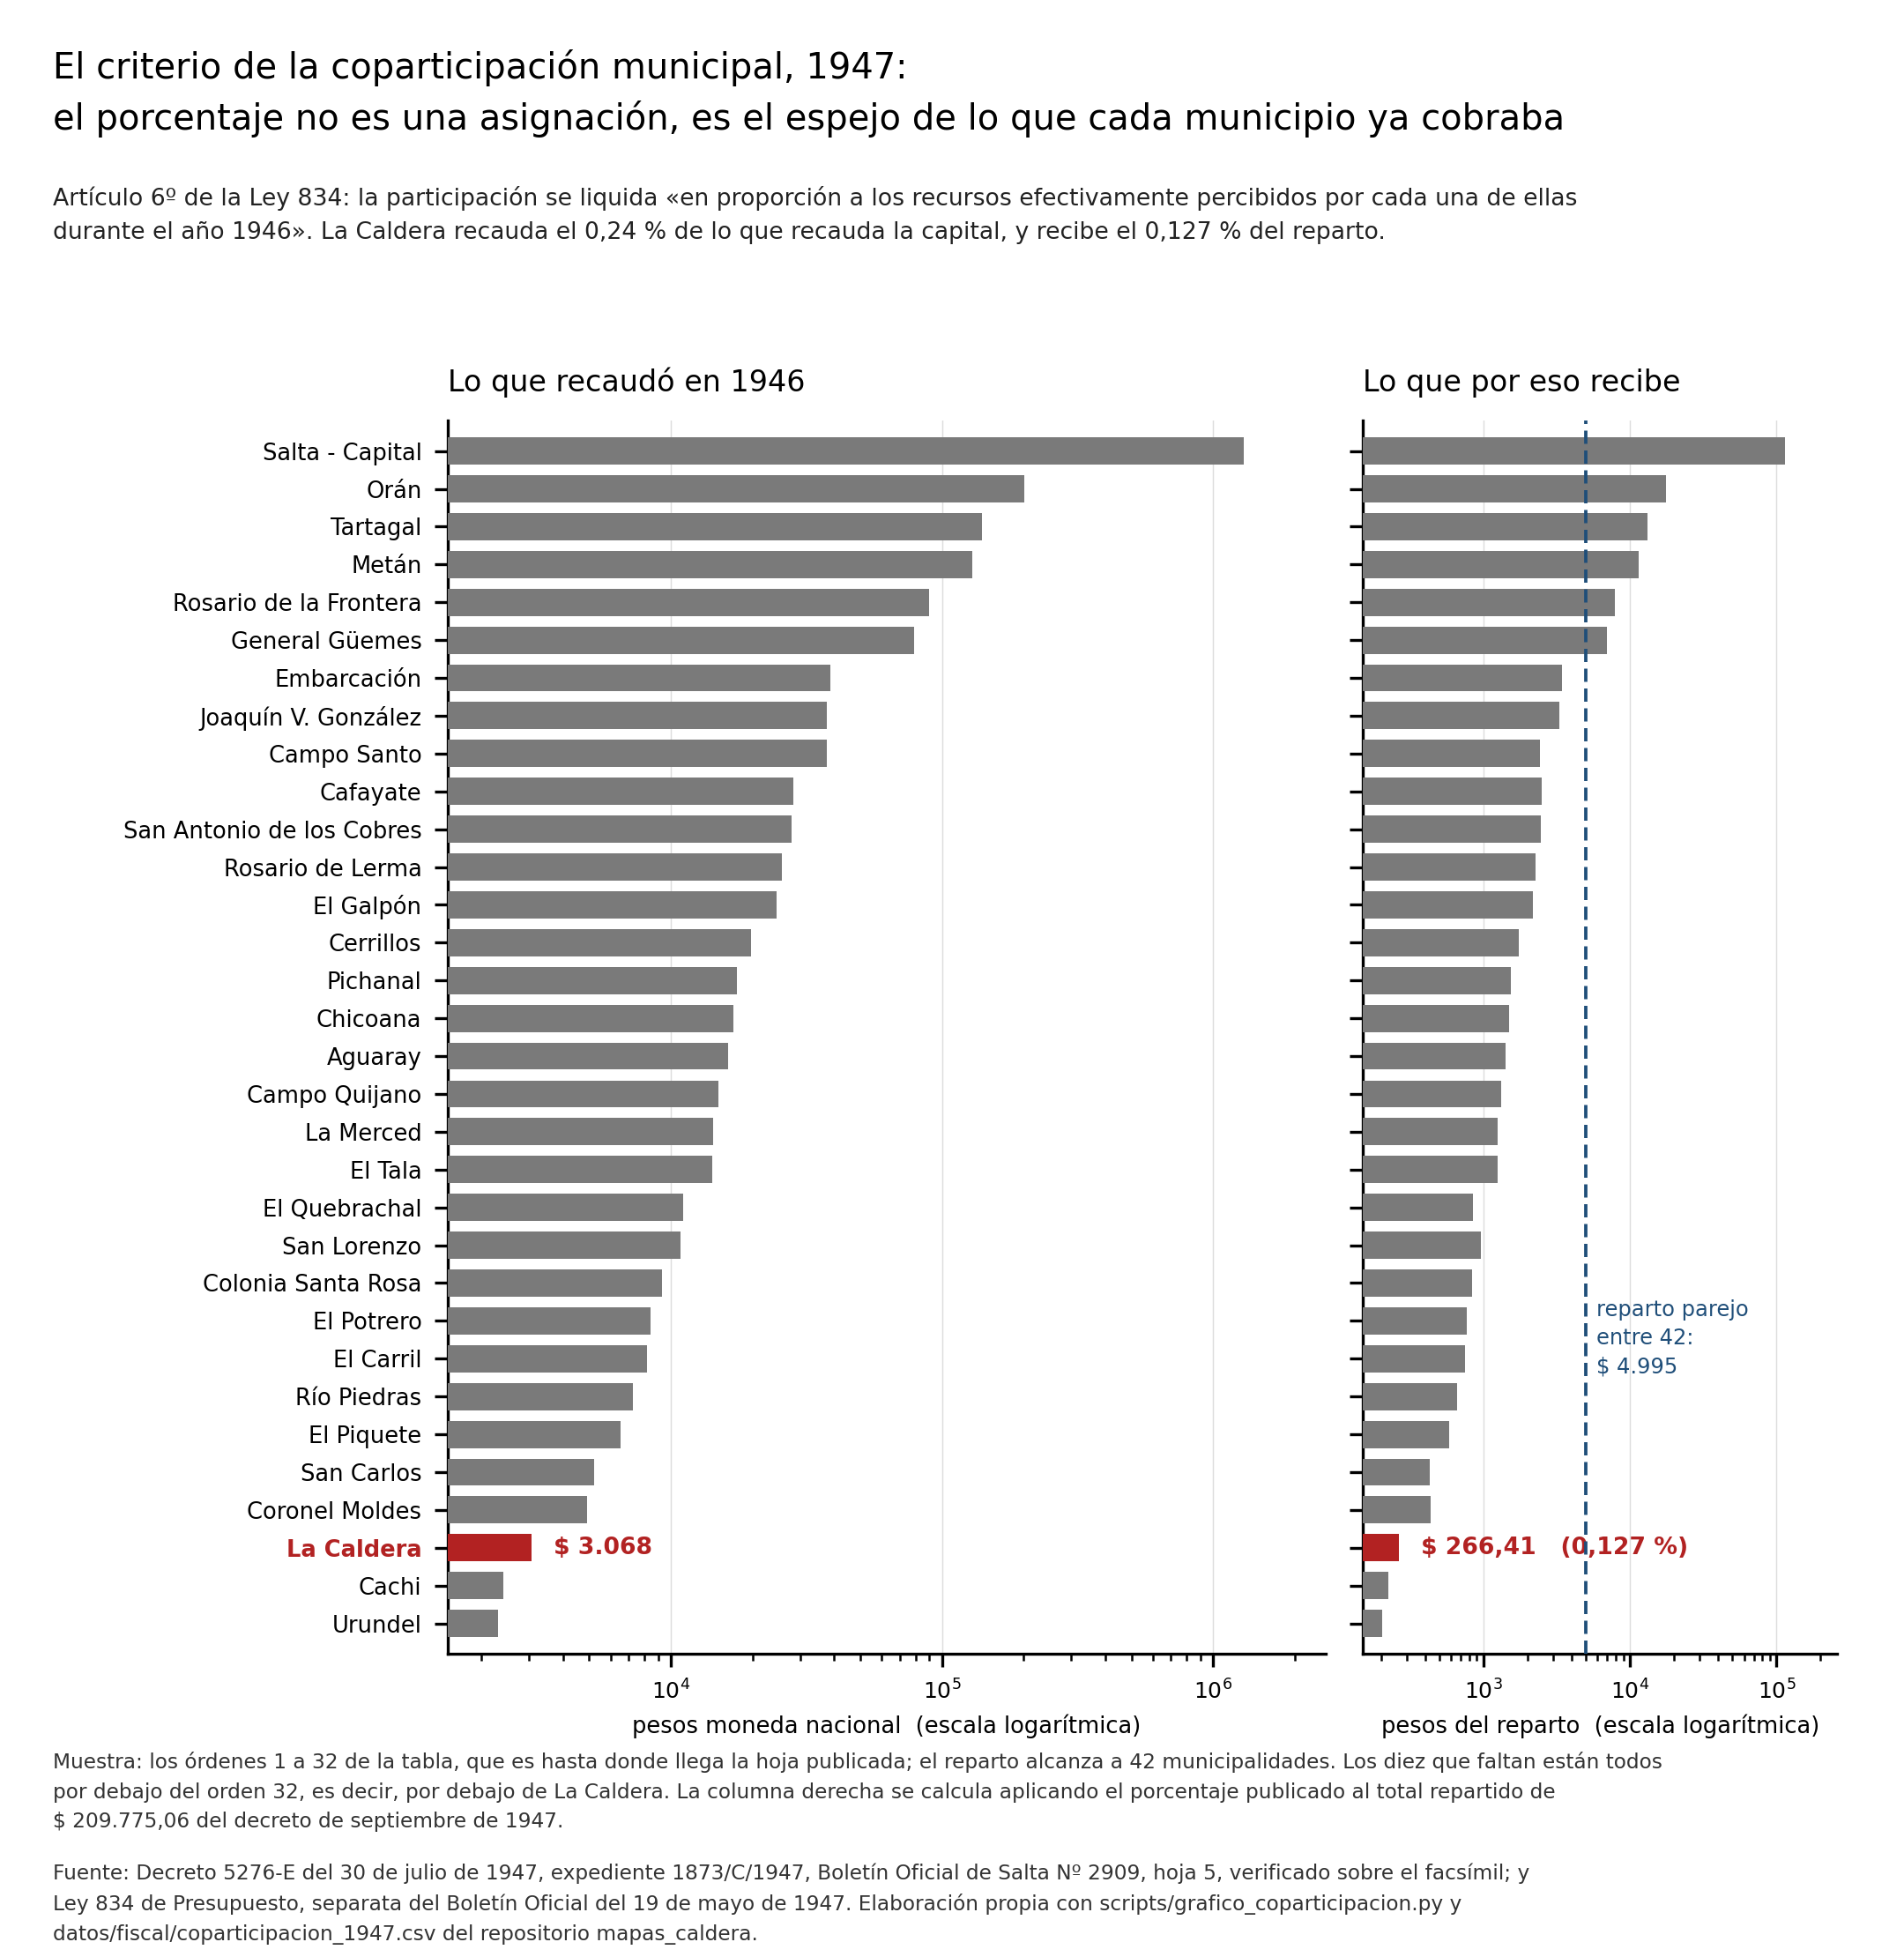
\includegraphics[width=\textwidth,height=0.88\textheight,keepaspectratio]{fig-coparticipacion-1947.png}
\caption[El criterio de la coparticipación municipal, 1947]{\textbf{El criterio de la
coparticipación municipal, 1947: el porcentaje no es una asignación, es el espejo de lo que cada
municipio ya cobraba.} Las dos columnas son la misma columna. El artículo 6º de la Ley 834 manda
liquidar la participación en los impuestos a los Réditos, Ventas, Beneficios Extraordinarios y
Contribución Territorial «\textit{en proporción a los recursos efectivamente percibidos por cada
una de ellas durante el año 1946}», de modo que \textbf{el que recauda poco recibe poco, y lo
recibe poco porque recauda poco}. La Caldera recaudó \$3.068 ---el 0,24 por ciento de lo que
recaudó la capital--- y le corresponde el \textbf{0,127 por ciento}: \$266,41 de los \$209.775,06
repartidos. La línea punteada marca dónde caería un reparto parejo entre las cuarenta y dos
municipalidades. \textbf{Muestra: los órdenes 1 a 32, que es hasta donde llega la hoja publicada;
los diez que faltan están todos por debajo de La Caldera.} Escala logarítmica en los dos paneles.
Fuente: Decreto 5276-E del 30 de julio de 1947, expediente 1873/C/1947, B.O.\ Nº 2909, h.\ 5,
verificado sobre el facsímil. Elaboración propia; dibujo de
\texttt{scripts/grafico\_coparticipacion.py} sobre \texttt{datos/fiscal/} del repositorio
\texttt{mapas\_caldera} (apéndice \ref{cap:fuentes}).}
\label{fig:coparticipacion}
\end{figure}

\begin{ficha}{1947--1948, lo que el Estado pone y lo que cobra}
\textbf{La escuela, y lo que costó pagarla.} El \textbf{decreto 12.581 del 19 de noviembre
de 1948} aprueba y adjudica «\textit{a la firma \textbf{Conrado Marcuzzi} la licitación de la
obra "Refecciones y ampliaciones en las instalaciones sanitarias de la \textbf{Escuela
Provincial de La Caldera}", por un importe total de \textbf{\$35.026,99}}». Ocho días
después, «\textit{atento a las observaciones formuladas por \textbf{Contaduría General}}», el
\textbf{decreto 12.744-E} ---dictado \textbf{en Acuerdo de Ministros} y firmado por tres---
\textbf{insiste} en el cumplimiento del anterior (B.O.\ Nº 3285, h.\ 6, verificado sobre el
facsímil). Y en diciembre de 1947 un acto autoriza al \textbf{Banco de Préstamos y Asistencia Social} a acordar «\textit{un subsidio extraordinario en la suma de \textbf{CIEN PESOS} a cada una de las \textbf{cooperadoras} de las escuelas nacionales y provinciales}» de toda la provincia. \textbf{El departamento entra con tres} (B.O.\ Nº 3022, h.\ 6, verificado sobre el facsímil): la \textbf{nacional Nº 51, Calderilla}, y las \textbf{provinciales Nº 21, La Caldera}, en el pueblo, y \textbf{Nº 22, Vaqueros}. Firman \textbf{Cornejo} y \textbf{José T.\ Solá Torino}.

\textbf{Tres escuelas, y la de Calderilla es nacional.} La distinción importa porque el
capítulo \ref{cap:presencia} mide qué pone la Provincia y qué pone la Nación: en 1947 el
departamento tiene \textbf{dos escuelas provinciales} ---el pueblo y Vaqueros--- y
\textbf{una nacional} en Calderilla. \textbf{Y el subsidio no va a las escuelas sino a sus
cooperadoras}, que es otra cosa: cien pesos a la asociación de padres, por una vez, y a través
de un banco. \textbf{Ese mismo año la Provincia presupuesta \$690.000 para un puente en el
mismo departamento.}

\textbf{Y una trampa que conviene dejar anotada}: la misma lista registra la escuela nacional
\textbf{Nº 212, «Entre Ríos»}, y no está en este departamento sino en \textbf{La Viña}. El
topónimo que este libro sigue desde 1909 ---la finca «Vaqueros o Entre Ríos»--- tiene
homónimo provincial, y cualquier búsqueda por nombre lo va a traer.

\textbf{Lo que el departamento recibe, con su denominador.} Un decreto de septiembre de 1947
reparte la \textbf{participación de la Ley nacional 12.956} entre \textbf{cuarenta y dos
municipalidades} de la provincia, por un total de \textbf{\$209.775,06}, con cargo a la cuenta
especial «\textit{Municipalidades de la Provincia}». \textbf{La Caldera figura en el orden 30
con \$266,41} (B.O.\ Nº 2932, h.\ 5, verificado sobre el facsímil), y otras ediciones del
bienio publican su coeficiente: \textbf{0,127 por ciento}, el mismo en 1947 y en 1948.

\textbf{Y el decreto que fija los porcentajes dice de dónde salen.} El \textbf{decreto 5276-E
del 30 de julio de 1947} (expte.\ 1873/C/1947), verificado sobre el facsímil, encadena tres
normas: el artículo 4º de la \textbf{Ley nacional 12.956} obliga a las provincias a distribuir
trimestralmente entre sus municipalidades «\textit{no menos del \textbf{10 \%} de la
participación que reciban de la Nación}»; el artículo 50 de la \textbf{Ley provincial 833} da
a los municipios «\textit{una participación del producto del Impuesto a la Contribución
territorial igual al \textbf{20 \%}}»; y el artículo 6º de la \textbf{Ley de Presupuesto 834} lo dispone.
\textbf{Ese artículo se leyó sobre la separata del Boletín, y no sólo en la cita del
decreto}: «\textit{Los proporcionales que sobre la recaudación del impuesto a los Réditos,
Ventas, y Beneficios Extraordinarios y Contribución Territorial le corresponde a las
Municipalidades de Salta y de la Campaña, serán liquidados \textbf{en proporción a los
recursos efectivamente percibidos por cada una de ellas durante el año 1946}. En lo que
respecta a la participación que le corresponde en el impuesto a los \textbf{Espectáculos
Públicos} éste será distribuido en proporción a la recaudación que del mismo efectúe cada
Municipalidad}».

\textbf{Y publica la tabla.} La recaudación propia de cada municipio en 1946, y el porcentaje
que de ella resulta: Salta capital, \textbf{\$1.298.124} y el \textbf{54,116 \%}; Orán,
\$201.982 y el 8,446; \ldots{} y \textbf{La Caldera, en el orden 30, \$3.068 y el
\textbf{0,127 \%}} (lámina \ref{fig:coparticipacion}). Por debajo sólo quedan Cachi, con \$2.406, y Urundel, con \$2.312.

\begin{cautela}
\textbf{El 0,127 por ciento no es una asignación: es un espejo.} La ley no reparte según
población ni según superficie ni según necesidad, sino \textbf{en proporción a lo que cada
municipio ya recaudaba por su cuenta}. \textbf{El que recauda poco recibe poco de lo que la
Nación manda}, y lo recibe poco \textit{porque} recauda poco.

\textbf{Este libro venía suponiendo que el coeficiente podía responder a población, a
superficie o a recaudación, y que el archivo no lo decía. Lo dice, y es la tercera.} La
regla está escrita en el artículo 6º de una ley de presupuesto, publicada, y con su tabla al
lado: cualquiera puede rehacer la cuenta. \textbf{Es un criterio explícito, y es regresivo por
construcción}: la coparticipación no corrige la asimetría entre municipios, la reproduce.

\textbf{Y la ley trae una segunda oración que el decreto no cita, y que aprieta más la
regla.} El impuesto a los \textbf{espectáculos públicos} se reparte «\textit{en proporción a
la recaudación que del mismo efectúe cada Municipalidad}». \textbf{Un departamento sin
cine, sin teatro y sin cancha con entrada recauda cero por ese impuesto, y por lo tanto recibe
cero.} No es que reciba poco: queda fuera del reparto. \textbf{Y eso vale para las dos
oraciones del artículo}, porque las dos reparten según lo que cada municipio ya cobra. La
diferencia es que en la primera el departamento entra con el 0,127 por ciento y en la segunda
no entra.

\textbf{Y fija el suelo del departamento en una cifra.} En 1946 el municipio de La Caldera
recaudó \textbf{\$3.068}, que es el \textbf{0,24 por ciento} de lo que recaudó la capital.
El capítulo \ref{cap:presencia} venía midiendo la presencia del Estado en el departamento por
lo que el Estado ponía; \textbf{ésta es la primera cifra de lo que el departamento ponía de sí
mismo}.

\textbf{Y hay un dato de ausencia en el mismo acto.} Su artículo 3º manda retener la parte
proporcional de los convenios que cuatro municipalidades ---\textbf{Salta, Metán, Rosario de
la Frontera y Campo Santo}--- celebraron con la Dirección Provincial de Sanidad. \textbf{La
Caldera no tiene convenio de sanidad}, y por eso no se le retiene nada: cobra menos y también
debe menos, que es la forma en que un departamento sin servicios aparece en una planilla.
\end{cautela}

\textbf{Y el plan hidráulico que no se publica.} El \textbf{decreto 5466-E del 14 de agosto
de 1947} (expte.\ 17847/1947) aprueba «\textit{provisoriamente el \textbf{plan hidráulico
orgánico de financiación y construcción de obras en el período 1948--1950} preparado por la
Administración General de Aguas de Salta y que representa en dicho período una inversión de
\textbf{\$35.100.000}}», por la resolución Nº 326 del acta Nº 16 del H.\ Consejo, del 18 de
julio de 1947, «\textit{y que corre de \textbf{fs.\ 12 a 18} del expediente precitado}». Se
dicta por el artículo 92 inciso i) del \textbf{Código de Aguas entonces vigente, la Ley
Nº 775}, y el considerando aclara que el plan «\textit{no se superpone con el plan de obras
previsto en el \textbf{Plan Quinquenal} del Superior Gobierno de la Nación}».

\begin{cautela}
\textbf{El acto publica el monto y no publica el plan.} Treinta y cinco millones de pesos para
obras hidráulicas en tres años, y qué obras, dónde y en qué orden queda en las fojas 12 a 18
de un expediente que el Boletín no reproduce. \textbf{Es, en 1947, la misma forma que el
capítulo \ref{cap:opacidad} documenta para los instrumentos de 2013 en adelante}: se publica
el marco y se reserva el contenido operativo.

\textbf{Y para este departamento la pregunta es precisa.} El capítulo viene siguiendo desde
1938 los intentos de defensa del río de la Caldera ---croquis en 1938, obra suspendida en
1940, licitación y ejecución por vía administrativa en 1945 por \$2.515--- y no sabe qué pasó
después. \textbf{Si esa defensa está en las fojas 12 a 18 de este plan, el hilo sigue; si no
está, se corta acá y el libro puede decirlo.} El apéndice \ref{cap:pedidos} pide esas siete
fojas.
\end{cautela}

\textbf{Y el presupuesto de 1947 sí pone plata en el río.} La \textbf{Ley 834}, que fija el
presupuesto provincial del año en \textbf{\$13.560.293,76}, trae en su \textbf{Ítem 6}
---«\textit{Obras de defensas permanentes o eventuales para contener daños por crecientes o
inundaciones sobre}»--- una lista de nueve ríos por un total de \textbf{\$560.000}. \textbf{Tres
de los nueve son de este departamento}: el \textbf{Mojotoro}, \textbf{\$100.000}; \textbf{La
Caldera}, \textbf{\$50.000}; y el \textbf{Wierna}, \textbf{\$50.000}, los tres en primera
etapa. Los otros seis son el Rosario (Toro), Chuñapampa, el Cachi, el Calchaquí, el Juramento y
el de Iruya, más \$60.000 de imprevistos (lámina \ref{fig:defensas}) (separata del B.O.\ del 19 de mayo de 1947,
págs.\ 141--142).

\begin{cautela}
\textbf{Doscientos mil pesos de quinientos sesenta mil: el 35,7 por ciento de todo lo que la
Provincia presupuesta en 1947 contra las crecientes va a los tres ríos de este departamento.}
Y los tres son uno solo: el acto de 1946 que este capítulo transcribe establece que el Mojotoro
forma su caudal con el Wierna, el de La Caldera y el Castellanos.

\textbf{Esto corrige lo que este libro venía dando por sentado.} El capítulo sigue los intentos
de defensa del río desde el croquis de 1938 y la obra suspendida de 1940 hasta la ejecución por
vía administrativa de 1945, \textbf{por \$2.515}, y la lectura implícita era que la Provincia no
ponía plata. \textbf{La ponía}: en 1947 hay una partida en la ley de presupuesto, votada por las
dos cámaras, de \textbf{veinte veces} lo gastado dos años antes, y el departamento concentra más
de un tercio del ítem provincial.

\textbf{Lo que no se sabe es si se ejecutó}, y ahí vuelve el patrón de este bienio: el mercado
presupuestado en julio y desafectado en diciembre, el camino objetado, el puente de \$690.000
sin licitación publicada. \textbf{Presupuestado no es ejecutado.} Y la pieza que podría
contestarlo son las fojas 12 a 18 del plan hidráulico 1948--1950, que el decreto 5466-E aprueba
sin publicar: \textbf{la partida de 1947 y el plan de 1948 son dos tramos del mismo expediente,
y de los dos se conoce el monto y no el destino.}
\end{cautela}

\textbf{Y la estación sanitaria vuelve, con otro origen.} El \textbf{Inciso VI} del mismo
presupuesto ---«\textit{Plan de obras con fondos de la \textbf{Ley Nº 770}}»--- destina
\textbf{\$370.000} a «\textit{estudios, proyectos y construcción de nuevos edificios para
\textbf{estaciones sanitarias}, sus instalaciones y amueblamiento, en las siguientes
localidades: El Tala; \textbf{La Caldera}; Pichanal; Joaquín V.\ González, Iruya, Santa
Victoria}». \textbf{Seis localidades en una sola partida}, sin decir cuánto le toca a cada una.
Es la \textbf{misma Ley 770} que financia el plan vial donde está el puente sobre el río, de
modo que \textbf{el puente y la estación sanitaria salen del mismo empréstito}, y el capítulo
\ref{cap:presencia} puede ahora nombrar la norma que paga lo que mide.

\textbf{El mercado que se presupuestó y se desafectó en el mismo año.} El decreto
\textbf{Nº 4945 del 1º de julio de 1947} destinó \textbf{\$600.000} a la construcción de
mercados en municipios, y entre ellos un \textbf{Mercado Tipo I para La Caldera}. En
diciembre, el decreto que adjudica los mercados de los demás departamentos
\textbf{«desaféctase provisoriamente»} el de La Caldera, junto con los de La Candelaria, La
Poma y San Carlos y el Tipo II de San Antonio de los Cobres, «\textit{para que con dicha
economía \ldots{} se haga viable la construcción de un \textbf{Mercado Frigorífico} en
\textbf{Embarcación}}» (B.O.\ Nº 3016, h.\ 9, verificado sobre el facsímil).

\begin{cautela}
\textbf{El motivo que el acto da es el que conviene leer despacio}: «\textit{a mérito de
considerarse ineficiosa la construcción de dichas obras en los pueblos antedichos,
\textbf{expresión que se había manifestado por los propios habitantes}}».

\textbf{El archivo no publica quién lo manifestó, cuándo ni por qué vía.} No hay nota, ni
petición, ni acta de la comisión municipal, ni expediente citado: la voluntad de los
habitantes aparece en el considerando de un decreto que les quita una obra, invocada por el
mismo organismo que la quita. \textbf{Es la única vez en el archivo temprano en que un acto
provincial dice hablar por los habitantes del departamento}, y lo hace para justificar una
desafectación. El apéndice \ref{cap:pedidos} pide el expediente.

\textbf{Y hay un antecedente exacto, tres años antes.} En mayo de 1944 el decreto 3016-H
aprueba la \textbf{eliminación del camino de Vaqueros a Los Yacones} del plan de obras de la
Ley nacional 12.776 (apéndice \ref{cap:cronologia}). \textbf{Dos obras presupuestadas para el
departamento y sacadas del plan en tres años}, mientras en 1947 los mercados sí se construyen
en Cerrillos, Rosario de Lerma, Campo Quijano, La Merced, San Lorenzo y Chicoana. \textbf{Lo
que el departamento recibe no es menos presupuesto: es más desafectación.}
\end{cautela}

\textbf{Y el contratista reaparece.} El mismo acto nombra a \textbf{Conrado Marcuzzi} entre
los oferentes que dieron cumplimiento al pliego. Es el mismo a quien, once meses después, se
le adjudica la obra sanitaria de la escuela del pueblo por \$35.026,99 ---la que necesitó una
insistencia en Acuerdo de Ministros para pagarse---.

\textbf{El camino, y la única objeción del Ejecutivo.} El \textbf{decreto 5916-E del 22 de
septiembre de 1947} aprueba el Acta Nº 188 del H.\ Consejo de Administración de Vialidad
\textbf{«a excepción de la resolución Nº 4967»}, y ordena que la Administración
«\textit{deberá informar en mérito a qué consideraciones ha sido incluido, \textbf{fuera del
plan}, el camino denominado «La Caldera a Santa Rufina», en la red de caminos
provinciales}» (B.O.\ Nº 2949, h.\ 12, verificado sobre el facsímil).

\textbf{El puente.} El \textbf{plan de obras de la Administración de Vialidad} de 1947
consigna «\textit{Puente S/Río La Caldera. Obras de arte Luz 150 mts.}» por
\textbf{\$690.000}, sobre un plan provincial total de \textbf{\$12.867.275,27}
(B.O.\ Nº 2983, h.\ 7, verificado sobre el facsímil).

\textbf{El Registro Civil, y quién fabrica sus muebles.} El \textbf{decreto 5537-G del 20 de
agosto de 1947} (expte.\ 6770/947) adjudica «\textit{a la \textbf{CÁRCEL PENITENCIARIA} la
confección de una mesa escritorio y tres sillas \ldots{} con destino a la Oficina de Registro
Civil de "La Caldera", al precio total de \textbf{ciento treinta y dos pesos con cuarenta}}»
(B.O.\ Nº 2923, h.\ 6, verificado sobre el facsímil).

\textbf{La salud, y un traslado que el libro no tenía.} El \textbf{decreto 9089-A del 8 de
abril de 1948}, verificado sobre el facsímil, dice: «\textit{Encontrándose vacante el cargo de
Enfermero del pueblo de \textbf{Rivadavia} \ldots{} nómbrase Auxiliar 7º (Enfermero de
Rivadavia) \ldots{} al actual Ayudante 5º (Enfermero de La Caldera), don \textbf{CLAUDIO
MURÚA}}»; y en su artículo 2º, «\textit{nómbrase Ayudante 5º (Enfermero de La Caldera), al
señor \textbf{TEODORO GÓMEZ}, en la vacante dejada por don Claudio Murúa}».

\textbf{La mina.} La \textbf{Resolución de Minas Nº 591}, del 2 de abril de 1948
---verificada sobre el facsímil, hoja 5---, adjudica «\textit{a favor del señor
\textbf{Enrique A.\ Zuccarino} y Sra.\ \textbf{María Josefina Méndez Alcorta de Zuccarino}
\ldots{} la presente mina de \textbf{plomo y plata} denominada "CALDERA No.\ 1, 2 y 3",
ubicada en el departamento de La Caldera, Exp.\ No.\ \textbf{44-L año 1929}}», por la última
parte del artículo 7º de la \textbf{Ley Nacional 10.273}. Firma \textbf{Luis Víctor Outes};
ante el escribano de minas \textbf{Oscar M.\ Aráoz Alemán}.
\end{ficha}

\begin{cautela}
\textbf{De toda el acta, lo único que el gobernador no aprueba es el camino del
departamento.} No lo rechaza: lo suspende y pide explicaciones, que es una figura distinta y
más rara. \textbf{Un camino entró a la red provincial por fuera del plan de obras}, y el
Poder Ejecutivo quiere saber con qué criterio. Es la primera vez en el archivo temprano que
un acto provincial \textbf{pregunta por el criterio} de una decisión sobre el departamento en
lugar de tomarla o publicarla, y este libro no tiene la respuesta: el apéndice
\ref{cap:pedidos} pide el informe que Vialidad debía elevar. \textbf{Santa Rufina}, además,
no es un destino cualquiera: la nómina electoral de 1948 la registra como paraje del circuito
del pueblo, y el apellido asociado a esa finca aparece en los pedimentos mineros de 1925.

\textbf{La escala del bienio, en una línea.} \$132,40 el mobiliario del Registro Civil,
\$35.026,99 los sanitarios de la escuela, \textbf{\$690.000 el puente}. \textbf{El puente
solo vale veinte escuelas y cinco mil doscientos Registros Civiles}, y es \textbf{el 5,4 por
ciento de todo el plan vial de la provincia}. El capítulo \ref{cap:presencia} mide el mismo
reparto para 1923--1945 y encuentra que lo único caro eran los caminos: 1947 y 1948 no lo
desmienten, lo confirman con tres cifras del mismo bienio, que \textbf{sí son comparables
entre sí} porque no median años de inflación ---las de 1934 no lo son, y este libro no las
corrige---.

\textbf{Y la escuela deja ver algo más.} La obra se adjudica el 19 de noviembre y ocho días
después el gobernador tiene que \textbf{insistir en Acuerdo de Ministros} contra las
observaciones de Contaduría General. \textbf{La partida más grande que el archivo temprano
destina a un edificio del departamento que no sea un camino necesitó saltar el control
contable para pagarse}, y el acto no dice cuál era la observación. El apéndice
\ref{cap:pedidos} la pide.

\textbf{Y la mina cierra una serie de diecinueve años, con tres datos que el libro no
tenía.} El expediente \textbf{44-L} es el que el padrón minero provincial cerrado el 30 de
marzo de 1933 registra bajo el número de orden 93, inscripto el 30 de abril de 1930 a nombre
de \textbf{Juan Larrán}: veintisiete hectáreas, tres pertenencias (capítulo
\ref{cap:siglo}).

\textbf{Primero: la mina es de plomo y plata}, y es la única sustancia metalífera que el
archivo temprano asocia a este departamento ---todo lo demás, antes y después, son áridos---.
\textbf{Segundo: las «tres pertenencias» del padrón de 1933 son las tres minas} que el acto
de 1948 nombra, «Caldera No.\ 1, 2 y 3». \textbf{Y tercero, el que importa: no se adjudica a
Larrán.} Entre la inscripción de 1930 y la adjudicación de 1948 el expediente cambió de
manos, y el acto no dice cuándo ni cómo: conserva el número de 1929 y nombra a otros dos.
\textbf{Diecinueve años entre inscribir y adjudicar}, y en el medio un traspaso que el
Boletín no publicó. El apéndice \ref{cap:pedidos} pide el expediente completo, que es lo
único que puede contar ese medio.

\begin{cautela}
\textbf{Murúa no deja el cargo: asciende y se va.} Pasa de \textbf{Ayudante 5º} en La Caldera
a \textbf{Auxiliar 7º} en Rivadavia, que es una categoría más alta y otro departamento.
\textbf{Es el primer caso documentado en el archivo temprano de un empleado del departamento
que sale de él por promoción}: todos los movimientos anteriores que este capítulo registra son
relevos dentro del departamento, ceses o intervenciones. \textbf{Y el que llega no viene de
ningún lado conocido}: Teodoro Gómez entra directamente en la vacante.
\end{cautela}

\textbf{Y \textit{Murúa} otra vez.} El apellido que este capítulo sigue desde 1912 ---jurado
de patentes, comisario en 1916, 1923, 1930 y 1932, causante del sucesorio que remata La
Calderilla en 1923, titular de La Despensa en 1925, miembro de la Comisión Municipal en 1938,
comisario en 1939 y nombrado en el expediente de pensión de 1941--- aparece en 1948 dejando
vacante el cargo de enfermero del departamento. \textbf{Coincidencia de nombre, como siempre.}

\textbf{Y en 1947 y 1948 el apellido aparece dos veces más, y las dos en los tribunales.} El
sumario de la edición 3019 de 1947 publica una \textbf{notificación de sentencia}
«\textit{en ejecución seguido por Banco Provincial de Salta vs.\ \textbf{Silvano U.\ Murúa} y
otros}» (aviso Nº 3347, h.\ 13 y 14); y el de la edición 3064 de 1948 abre el
\textbf{juicio sucesorio} «\textit{de don \textbf{Silvano, I.\ O.\ Ignacio Murúa}}» (aviso
Nº 3442, h.\ 12). \textbf{Los dos avisos se verificaron sobre el facsímil} ---son de las
hojas de sumario que el repositorio sí recortó---. Un ejecutado por el banco provincial en
diciembre de 1947 y un sucesorio abierto al año siguiente: \textbf{el archivo no dice que
sean la misma persona, y este libro tampoco}, pero el apellido que administró el
departamento desde 1912 termina el bienio en ejecución y en sucesión.
\end{cautela}

\subsection*{Una trampa de homonimia dentro del propio archivo}

\textbf{Las dos puntas están verificadas sobre el facsímil}, y dicen esto.

La \textbf{Resolución Nº 423-E} del 7 de noviembre de 1947 (expte.\ 18646/47; B.O.\ Nº 2985,
h.\ 7) autoriza una nota de crédito de \textbf{\$541,20} «\textit{a favor del Receptor de
Rentas de la localidad de La Caldera, \textbf{Departamento de la Capital}, don GERARDO
GUERRERO}», por estampillas «\textit{aplicadas \textbf{por error} en las boletas de
Contribución Territorial}». La adscripción a Capital \textbf{aparece dos veces en el mismo
acto}, en el visto y en la parte resolutiva, de modo que no es un desliz de una línea.

El \textbf{Decreto Nº 8706-E} del 10 de marzo de 1948 (expte.\ 4567/F/1948; B.O.\ Nº 3083,
h.\ 5) «\textit{desígnase Receptor de Rentas y Expendedor de Guías, Transferencia de Cueros
Marcas y Señales, y Multas Policiales del \textbf{Departamento de La Caldera}, al señor
GERARDO GUERRERO}». Y lo hace «\textit{atento a lo solicitado por el \textbf{Banco Provincial
de Salta}}».

\begin{cautela}
\textbf{El acto de 1948 no confirma al de 1947: lo designa de nuevo.} Cuatro meses después de
cobrar como receptor de una localidad del departamento Capital, el mismo hombre es
\textbf{designado} receptor del departamento de La Caldera. Caben las dos lecturas ---que el
Boletín se equivocó dos veces en 1947, o que Guerrero cambió de destino--- y este libro no
elige: registra las dos y pide el legajo.

\textbf{Y sobre quién pide la designación, este libro se corrige a sí mismo.} Que la pida el
\textbf{Banco Provincial de Salta} parecía una anomalía ---no la piden el municipio, ni la
Dirección General de Rentas, ni la policía, que son los tres organismos cuyos ingresos el
cargo recauda---. \textbf{No lo es, y el propio archivo lo explica cuatro meses antes.} El
\textbf{decreto 5919-E del 22 de septiembre de 1947} (expte.\ 2376/B/47) designa a los
expendedores de guías de \textbf{Orán} y de \textbf{Campo Santo} con la misma fórmula
---«\textit{atento lo solicitado por el Banco Provincial de Salta \ldots{} y lo dispuesto por
el art.\ 3º de la \textbf{Ley Nº 744}}»--- y dice para qué: cada designado «\textit{deberá
prestar \textbf{fianza a satisfacción del Banco Provincial de Salta}}».

\textbf{El banco no elige al recaudador: es ante quien el recaudador afianza.} La solicitud
es el trámite que el artículo 3º de la Ley 744 le asigna, y no una preferencia. Lo que en un
solo acto parecía una decisión bancaria sobre un departamento, visto en serie es un
procedimiento provincial que se aplica igual en tres departamentos distintos.
\textbf{Registrarlo así es el punto}: un acto aislado se lee mal, y la serie corrige la
lectura.
\end{cautela}

\subsection*{La decimotercera nómina, y lo que le hace a la lámina}

El \textbf{Decreto 8176 del 5 de febrero de 1948} fija ubicación y circuitos de los colegios
electorales 1 a 6 ---«\textit{La Capital, La Caldera, Campo Santo, Metán, Anta y
Rivadavia}»---, y el del departamento se publica entero, repetido en seis ediciones
seguidas (B.O.\ Nº 3060 a 3065; el sumario lo lista bajo el aviso Nº 3459, hoja 3).
\textbf{Verificado sobre el facsímil} de la hoja 19 de la edición 3062.

\textbf{La Caldera es el Colegio Electoral Nº 2}, y tiene dos circuitos.

\textbf{El circuito Nº 5} es el pueblo y el interior, con tres mesas: dos en la escuela
elemental mixta y una en la iglesia parroquial. Las mesas 1 y 3 votan
\textbf{Calderilla, Chalchanio, Helvecia, Getsemaní, Peñones, Potrero de Castilla, Pueblo,
San Alejo y Severino}. La mesa 2, \textbf{Abra de la Sierra, Acheral, El Angosto, Angosto
de Arrieta, Angostura, El Bordo, Calderilla, Campo Alegre, Cañada Ancha, Corral de
Barranca, Churcal, Los Chusos, Despensa, Despensilla, Higueritas, Potrero de Gallinato,
Las Lagunas, Los Matos, Mesada, Monte de las Garrapatas, Mosquera, Nogalito, Potrero de
Valencia, Los Porongos, Quesería, Santa Gertrudis, Santa Rufina, Los Sauces, La Sierra,
Wierna y Yacones}.

\textbf{El circuito Nº 6 es Vaqueros}, con dos mesas ---la Escuela Infantil Provincial y el
Hogar Agrícola «San Cayetano»--- y siete nombres: \textbf{Entre Ríos, Estación
F.\ C.\ C.\ N.\ A., Mojotoro, Lesser, El Túnel, Vaqueros y Villa Urquiza}.

\begin{cautela}
\textbf{Es la decimotercera nómina del mismo territorio, y la primera posterior a 1940.} La
lámina \ref{fig:parajesnom} reúne \textbf{doce} nóminas oficiales entre 1909 y 1940 y da
cincuenta y dos nombres distintos. \textbf{Esta no está en la lámina}, y hasta que se
incorpore ---lo que exige rehacer la tabla con el script que la produce, sobre el facsímil y
no sobre la capa de texto--- las dos afirmaciones que la lámina sostiene quedan acotadas a
1909--1940 y no al archivo temprano entero.

\textbf{Lo que ya se puede decir es que la lista de 1948 trae nombres que las doce no
traían}: \textbf{Helvecia} ---que es la Calderilla rebautizada, y aparece como paraje el mismo
año en que pide agua---, \textbf{Getsemaní} ---que el deslinde de 1916 nombraba como propiedad
de Daniel Linares, el mismo que en 1948 pide el agua de El Angosto, y no como paraje---, \textbf{Severino}, \textbf{Abra de la Sierra},
\textbf{Cañada Ancha}, \textbf{Corral de Barranca}, \textbf{Churcal}, \textbf{Los Chusos} y
\textbf{El Bordo}. \textbf{Y trae los que no se mueven}: Calderilla, Campo Alegre, San Alejo,
Potrero de Castilla, Peñones, Wierna y Yacones, que estaban en las doce.

\textbf{Y el Tribunal Electoral publica quiénes presiden las mesas.} Para los dos circuitos
del departamento designa \textbf{quince personas} ---presidente y dos suplentes por cada una de
las cinco mesas--- (B.O.\ Nº 3069, h.\ 14, verificado sobre el facsímil). \textbf{Este libro no
las transcribe}: son designaciones de 1948 y, por la regla de los cien años que el capítulo
\ref{cap:metodo} fija, esas personas se presumen vivas. Se nombra una sola, porque el
argumento la necesita.

\begin{cautela}
\textbf{En la mesa 2 del circuito de Vaqueros, el suplente segundo es un \textit{Urquiza}.}
Veinticuatro años antes, en 1924, \textbf{Francisco S.\ Urquiza} era presidente de mesa
electoral en Vaqueros, y ése era uno de los cinco roles simultáneos que este capítulo le
documenta. \textbf{Y la nómina de parajes del mismo decreto de 1948 registra \textit{Villa
Urquiza} como uno de los siete nombres del circuito.}

\textbf{Coincidencia de apellido, con la regla de siempre}: el libro no afirma parentesco ni
identidad. \textbf{Lo que sí queda registrado es que el apellido está en los tres lugares a la
vez} ---en el topónimo, en la mesa electoral y en la serie de 1924--- y que el lugar es el
mismo. Es el patrón que el capítulo viene siguiendo desde 1909, y en 1948 sigue en pie.
\end{cautela}

\textbf{Y el circuito Nº 6 contesta una pregunta que este libro traía abierta desde 1909}:
dónde cae la finca \textbf{Entre Ríos}. Cae en Vaqueros, y encabeza su nómina. La
«\textit{Vaqueros o Entre Ríos}» de los remates y los deslindes es, en 1948, el primer
paraje de su propio circuito electoral. Y con ella aparecen dos nombres que el archivo
temprano no traía: \textbf{El Túnel} ---la obra del ferrocarril, convertida en topónimo--- y
\textbf{Villa Urquiza}, que es la primera vez que el archivo nombra una \textit{villa} en el
departamento.

\textbf{El circuito electoral parte al departamento en dos
veintidós años antes de que la ley cree el segundo municipio}, y ocho meses después de que el
acto de límites de 1947 declarara que el municipio de La Caldera abarca el departamento
entero. \textbf{Las dos cosas son del mismo Estado y del mismo bienio.}
\end{cautela}


\section{1949: la obra que sí se hizo, y el decreto que se la dio a otro}

El año se leyó edición por edición y es el \textbf{trigésimo quinto tramo}: \textbf{281
archivos} y \textbf{4.869 hojas}, el más voluminoso de toda la serie temprana. Rige la misma
reserva que para 1947 y 1948 ---barrido automático, \textbf{sin lectura sobre la imagen} salvo
las hojas que el apéndice \ref{cap:fuentes} enumera---, y las tapas repiten la patología de
1947: el lector devuelve «Nº 4780» tres veces, «Nº 1805», y fechas imposibles como
«1349-01-07» y «3949-01-20». \textbf{El número de edición de la tapa no es confiable en 1949};
se toma del nombre del archivo.

\begin{ficha}{\textbf{Decreto Nº 13793-E} del 31 de enero de 1949, orden de pago 501, expediente 404/E/1949 (B.O.\ Nº 3337, h.\ 11)}
\textbf{Verificado sobre el facsímil.} «\textit{Apruébase el certificado No.\ 1 \ldots{} por
trabajos ejecutados en la obra: \textbf{Estación Sanitaria en La Caldera}, por la Empresa
\textbf{E.C.O.R.M.\ S.R.L.}, el que asciende a la suma de \textbf{\$27.024,10} \ldots{}
adjudicada al contratista Empresa E.C.O.R.M.\ S.R.L.\ \textbf{por decreto No.\ 10668 del 29 de
julio de 1948}}».

El artículo 3º manda retener el \textbf{10 por ciento} en concepto de garantía de obra, y el
4º imputa el gasto al \textbf{Anexo I, Inciso III, Principal 1/c} del presupuesto de 1948.
Ediciones posteriores del mismo año publican el acta «\textit{para la entrega de la obra}».
\end{ficha}

\begin{cautela}
\textbf{Este libro se corrige.} La sección anterior sostiene que el bienio 1947--1948 es de un
Estado que presupuesta y retira, y enumera cuatro obras de las que tres salieron del plan.
\textbf{La cuarta no salió: se hizo.} La estación sanitaria estaba en el Inciso VI de la Ley
834 de mayo de 1947, dentro de los \$370.000 repartidos entre seis localidades; se
\textbf{adjudicó el 29 de julio de 1948}; su primer certificado se pagó el 31 de enero de 1949;
y se entregó ese año. \textbf{La cadena completa está publicada, acto por acto, y se puede
seguir.}

\textbf{De modo que el patrón existe pero no es una ley, y conviene decir de qué depende.} Lo
que se cayó fue el mercado, el camino y el puente ---obra pública de fomento y de
infraestructura---. Lo que se hizo fue la escuela y la estación sanitaria. \textbf{En este
departamento, en este bienio, lo que el Estado termina es lo que atiende cuerpos.}
\end{cautela}

\subsection*{Y en la misma página está el mercado que no se hizo}

El decreto que aprueba el certificado de la estación sanitaria comparte hoja con otro que
aprueba el certificado parcial Nº 1 de la obra «\textit{\textbf{Mercado Tipo II en
Pichanal}}», por \textbf{\$9.783,82}, «\textit{trabajos adjudicados al señor Arquitecto
\textbf{Luis Moreno Díaz} por \textbf{decreto Nº 7321 del 13 de diciembre de 1947}}».

\begin{cautela}
\textbf{Ése es el mismo decreto que desafectó el mercado de La Caldera.} El acto del 13 de
diciembre de 1947 que quitó el Mercado Tipo I de este departamento ---«\textit{a mérito de
considerarse ineficiosa la construcción de dichas obras en los pueblos antedichos, expresión
que se había manifestado por los propios habitantes}»--- es el que \textbf{adjudicó el de
Pichanal}. Y en febrero de 1949 el de Pichanal se está certificando y pagando.

\textbf{No son dos decisiones: es una.} La economía que justificó la desafectación de cinco
mercados ---La Caldera, La Candelaria, La Poma, San Carlos y San Antonio de los Cobres--- es
la que financió los que sí se construyeron. \textbf{El mismo número de decreto está en las dos
puntas}, y el archivo lo publica en la misma página trece meses después. Lo que el libro no
tiene es la constancia de esa expresión de los habitantes, que el apéndice
\ref{cap:pedidos} reclama.
\end{cautela}

\subsection*{El río La Caldera pasa a ser el primero de la provincia}

El presupuesto de 1949 repite la estructura de la Ley 834, y su \textbf{Ítem 6} ---las obras de
defensa contra crecientes--- reparte \textbf{\$460.000} entre diecisiete ríos y un renglón de
imprevistos, cien mil menos que en 1947 (B.O.\ Nº 3341, h.\ 12, verificado sobre el facsímil).
El reparto del departamento cambia de forma:

\begin{center}
\small
\begin{tabular}{lrr}
\toprule
 & \textbf{1947} & \textbf{1949} \\
\midrule
La Caldera              & 50.000  & \textbf{80.000} \\
Mojotoro                & 100.000 & 50.000 \\
Wierna                  & 50.000  & 10.000 \\
Vaqueros                & ---     & 10.000 \\
\midrule
\textbf{Del departamento} & \textbf{200.000} & \textbf{150.000} \\
Total del ítem          & 560.000 & 460.000 \\
Participación           & 35,7 \% & 32,6 \% \\
\bottomrule
\end{tabular}
\end{center}

\begin{cautela}
\textbf{Con ochenta mil pesos, el río de la Caldera es la partida más alta de las dieciocho del
ítem}, por encima de Iruya, del Colorado y de San Antonio de los Cobres. \textbf{Y Vaqueros
aparece como río propio por primera vez}: en 1947 el presupuesto lo contaba dentro del
Mojotoro, y en 1949 tiene su renglón. \textbf{Es la primera vez que un instrumento provincial
separa a Vaqueros del sistema}, veintiún años antes de que la ley lo separe como municipio.

\textbf{La participación del departamento baja y su río sube}, que no es lo mismo: el ítem
entero se achicó, el Mojotoro y el Wierna perdieron la mitad y cuatro quintos, y lo que quedó
se concentró en el río del pueblo. \textbf{Este libro no sabe si esos ochenta mil se
ejecutaron}, y por las mismas razones de siempre: el archivo publica el presupuesto y no el
certificado.

\textbf{Y hay un segundo ítem con el departamento adentro.} El \textbf{Ítem 5} destina
\textbf{\$120.000} a «\textit{expropiación, estudios, proyectos, conservación y refección de
servicios de extensión y reducido (con captación superficial), en las siguientes localidades:
El Tala, Tolombón, Molinos, \textbf{La Caldera}, La Poma, Iruya y otras localidades de la
Provincia (obras de fomento)}».
\end{cautela}

\subsection*{La mina se adjudica por segunda vez}

\begin{ficha}{\textbf{Resolución de Minas Nº 672}, del 10 de febrero de 1949 (B.O.\ Nº 3346, h.\ 9)}
\textbf{Verificada sobre el facsímil.} «\textit{Y VISTOS: El escrito que antecede y de acuerdo
con lo dispuesto por la Ley Nacional 10.273, art.\ 7º, \textbf{in fine}, adjudícase a favor del
señor \textbf{Enrique A.\ Zuccarino} y señora \textbf{María Josefina Méndez Alcorta de
Zuccarino}, la mina de plomo y plata denominada "Caldera 1, 2 y 3", ubicada en el Departamento
del mismo nombre, \textbf{lugar denominado San José}, Exp.\ No.\ 44---L, año 1929}».
\end{ficha}

\begin{cautela}
\textbf{Es la misma adjudicación de diez meses antes, palabra por palabra}, incluida la
invocación del artículo 7º \textit{in fine} de la Ley 10.273: la Resolución Nº 591 del 2 de
abril de 1948 ya la había dictado, con los mismos adjudicatarios y el mismo expediente.
\textbf{Dos adjudicaciones idénticas del mismo derecho, con diez meses de diferencia}, y el
Boletín no publica nada en el medio. O la primera no se registró, o no quedó firme, o hubo un
trámite que no se publicó; el expediente 44-L es lo único que puede decirlo, y el apéndice
\ref{cap:pedidos} lo pide.

\textbf{Y la resolución de 1949 trae un dato que la de 1948 no tenía: el lugar.} La mina está
en «\textbf{San José}», que \textbf{no figura entre los parajes de la nómina electoral de
1948} ---donde sí están San Alejo, Santa Rufina y Santa Gertrudis---. Es el único dato de
ubicación que el archivo da de esta mina en veinte años.
\end{cautela}


\section{1950: se cierra la obra y se fracciona Entre Ríos}

El año se leyó edición por edición y es el \textbf{trigésimo sexto tramo}: \textbf{277
archivos} y \textbf{4.156 hojas}, con la misma reserva que los tres anteriores.

\subsection*{La estación sanitaria se recibe}

En la edición \textbf{3684} se aprueba otro certificado por trabajos ejecutados, y en la
\textbf{3864} el trámite se cierra: se devuelven «\textit{los certificados correspondientes a
la obra "estación sanitaria tipo "A" en La Caldera", \textbf{con imputación a la cuenta
especial "Depósitos en garantía"}}», a favor de la empresa constructora E.C.O.R.M.\ S.R.L.

\begin{cautela}
\textbf{Ésa es la devolución de la retención del diez por ciento, y por lo tanto la recepción
definitiva.} La cadena queda completa y publicada, acto por acto, a lo largo de cuatro años:
presupuestada en el Inciso VI de la Ley 834 en \textbf{mayo de 1947}; adjudicada por decreto
10668 el \textbf{29 de julio de 1948}; primer certificado pagado el \textbf{31 de enero de
1949}; entregada ese año; garantía devuelta en \textbf{1950}.

\textbf{Es la única obra del departamento que el archivo temprano permite seguir de punta a
punta}, y conviene medir lo que eso significa. El capítulo \ref{cap:presencia} venía
sosteniendo que de los edificios públicos del departamento sólo se puede seguir la historia
completa de uno, y era aquel que el Estado ocupaba sin título desde hacía treinta años.
\textbf{Ahora son dos, y el segundo es el que se hizo bien.}
\end{cautela}

\subsection*{Y aparece la palabra «fracción»}

Tres ediciones seguidas ---\textbf{3692, 3693 y 3694}--- publican el mismo edicto de la
Administración General de Aguas: alguien solicita reconocimiento de concesión sobre la
propiedad «\textit{denominada \textbf{"Fracción Entre Ríos"}, ubicada en \textbf{Vaqueros},
departamento de La Caldera}», y «\textit{el reconocimiento a otorgarse sería para una dotación
de agua proveniente}» del sistema. El aviso invoca además el \textbf{decreto Nº 3649 del 11 de
julio de 1944}.

\begin{cautela}
\textbf{«Fracción Entre Ríos» no es «Entre Ríos».} La finca que este libro sigue desde los
remates de 1909, que da nombre al municipio de Vaqueros y que en 1948 encabeza la nómina de su
circuito electoral, \textbf{en 1950 ya está dividida}, y una de sus partes pide agua con nombre
propio. \textbf{Es la primera vez que el archivo temprano nombra una fracción de una finca de
este departamento}: hasta acá las fincas aparecían enteras, deslindadas y mensuradas, pero
nunca partidas.

\textbf{Y el agua llega antes que el plano.} El capítulo \ref{cap:loteo} documenta para los
loteos recientes que el orden habitual es el inverso ---primero el fraccionamiento aprobado,
después los servicios---, y acá el reconocimiento de agua sobre una fracción se publica sin
que el Boletín haya publicado antes su plano. \textbf{Este libro no afirma que no exista}: el
plano puede estar en Dirección General de Inmuebles sin pasar por el Boletín, que es
exactamente lo que el capítulo \ref{cap:opacidad} describe. El apéndice \ref{cap:pedidos}
pide el expediente y el plano de esa fracción.
\end{cautela}

\section{Qué hace el bienio 1947--1948, y por qué no es más de lo mismo}

Los dos años que este capítulo acaba de incorporar no aportan un hallazgo suelto: aportan
\textbf{una forma de operar que los treinta y dos tramos anteriores no mostraban junta}. Vale
la pena enunciarla, con la reserva de que \textbf{los dos años entraron al libro por lectura
de capa de texto} y que, de las hojas que sostienen lo que sigue, este libro verificó sobre el
facsímil las que el apéndice \ref{cap:fuentes} enumera y no las demás.

\begin{cautela}
\textbf{No es un bienio de ausencia de Estado. Es uno de Estado que presupuesta y retira.}

\textbf{El mercado.} El decreto 4945 del 1º de julio de 1947 destina \$600.000 a mercados
municipales y prevé uno \textbf{Tipo I para La Caldera}. En diciembre, el mismo Estado lo
\textbf{desafecta} y pasa el dinero al Mercado Frigorífico de Embarcación, «\textit{a mérito
de considerarse ineficiosa la construcción \ldots{} expresión que se había manifestado por los
propios habitantes}». \textbf{Los mercados sí se construyen} en Cerrillos, Rosario de Lerma,
Campo Quijano, La Merced, San Lorenzo y Chicoana.

\textbf{El camino.} El decreto 5916-E aprueba el Acta 188 del Consejo de Vialidad
\textbf{«a excepción de la resolución Nº 4967»}, la única que exceptúa, y exige que se informe
por qué el camino «\textit{La Caldera a Santa Rufina}» entró \textbf{fuera del plan} a la red
provincial.

\textbf{El puente.} El plan vial de 1947 lo presupuesta en \textbf{\$690.000} ---el 5,4 por
ciento de todo el plan provincial--- y el archivo no publica después ni licitación ni
adjudicación ni certificado.

\textbf{La escuela.} La única obra del bienio que llega a ejecutarse, \$35.026,99 en
sanitarios, \textbf{necesita una insistencia en Acuerdo de Ministros} contra las observaciones
de Contaduría General para poder pagarse.

\textbf{Y hay antecedente.} En mayo de 1944 el decreto 3016-H aprueba \textbf{eliminar el
camino de Vaqueros a Los Yacones} del plan de la Ley nacional 12.776. \textbf{Cuatro obras
presupuestadas para este departamento en cinco años, y tres salen del plan.}

\textbf{La cuarta es la excepción y hay que decirla acá, no sólo después.} La estación
sanitaria del Inciso VI se adjudicó en julio de 1948, se certificó en enero de 1949 y se
entregó ese año, con toda su cadena publicada (sección siguiente). \textbf{De modo que la
frase correcta no es que el Estado presupuesta y retira, sino que retira lo que construye y
termina lo que atiende}: se cayeron el mercado, el camino y el puente; se hicieron la escuela
y la estación sanitaria.
\end{cautela}

\begin{cautela}
\textbf{Y el criterio, cuando está escrito, es regresivo.}

El artículo 6º de la Ley de Presupuesto 834 manda liquidar la coparticipación municipal
«\textit{en proporción a los recursos efectivamente percibidos por cada una de ellas durante
el año 1946}», y el decreto 5276-E publica la tabla entera: \textbf{lo que cada municipio
recaudó y el porcentaje que le toca}. La Caldera recaudó \textbf{\$3.068} y le corresponde el
\textbf{0,127 por ciento}; la capital recaudó \$1.298.124 y le corresponde el 54,116.

\textbf{Este libro sostiene que la opacidad de este dispositivo opera en el nivel del criterio
y no del acto, y éste es el contraejemplo que hay que poner.} Acá el criterio está escrito, es
público y su tabla está al lado: cualquiera puede rehacer la cuenta. \textbf{Que se pueda leer
no lo vuelve menos duro. Lo vuelve discutible}, que es exactamente lo que el capítulo
\ref{cap:opacidad} reclama para los instrumentos de 2013 en adelante y no obtiene.

\textbf{Y hay un segundo criterio, éste no enunciado pero deducible.} Los dos reconocimientos
de agua del bienio publican la superficie y el caudal: 24 hectáreas y 12,6 litros por segundo
para La Helvecia, 29 y 15,22 para El Angosto. \textbf{Las dos razones dan 0,525 litros por
segundo por hectárea.} Nadie escribió «0,525» en ningún lado, pero \textbf{publicar los dos
términos de la división vuelve verificable la regla sin necesidad de enunciarla}.

\textbf{De modo que el archivo de 1947--1948 ofrece las tres posiciones posibles}: un criterio
escrito y publicado (la coparticipación), uno no escrito pero reconstruible (el agua), y uno
retenido (las fojas 12 a 18 del plan hidráulico de \$35.100.000, que el decreto 5466-E aprueba
sin publicar). \textbf{La tercera posición es la que el resto del libro documenta para los
ochenta años siguientes}, y encontrar las otras dos conviviendo con ella en el mismo bienio
obliga a decir que la opacidad de criterio \textbf{no es una condición del Estado provincial
sino una elección que se toma acto por acto}.
\end{cautela}

\begin{cautela}
\textbf{Y los nombres de 1916 vuelven en 1948.}

\textbf{Hermann Pfister}, el perito que deslindó Loma Bola, Santa Mónica, Quitilipe y el
Potrero Gallinato en 1916 y 1917, pide en 1948 el agua del río para La Helvecia.
\textbf{Daniel Linares}, a quien el deslinde de 1916 nombra como propietario de Getsemaní,
pide el agua para El Angosto. \textbf{Los dos peticionantes de agua del bienio salen de los
deslindes de treinta años antes.} Y un \textbf{Urquiza} vuelve a ser autoridad de mesa
electoral en Vaqueros, veinticuatro años después de que Francisco S.\ Urquiza acumulara allí
cinco roles, en el circuito donde el mismo decreto registra el paraje \textbf{Villa Urquiza}.

\textbf{Coincidencia de apellido, con la regla de siempre}, y por eso este libro no afirma
identidad ni parentesco. \textbf{Lo que afirma es más simple y más verificable}: que el
conjunto de apellidos que aparece midiendo y poseyendo la tierra en 1916 es el mismo que
aparece pidiendo su agua y presidiendo sus mesas en 1948. \textbf{El que mide, el que posee y
el que administra no son tres conjuntos distintos en este departamento}, y eso el capítulo lo
venía diciendo para 1909 y 1924. \textbf{1948 muestra que todavía vale cuando el archivo se
cierra.}
\end{cautela}


\section{Y la tierra cambiaba de manos}

En julio de 1922, el mismo martillero que tres años después remataría la fundición anuncia
otra venta: «por disposición del señor Juez de Primera Instancia Dr. Mendioroz y como
correspondiente a la ejecución seguida por el Dr. Marcos Alsina contra don José Nogales,
venderé con base de \$800 la finca denominada Potrero del Gallinato, ubicada en el
Departamento de La Caldera y de propiedad del ejecutado».

\textbf{Y hay un acto anterior, que explica quién era el ejecutado.} En enero de 1917, Camilo
Cáceres pide el deslinde, la mensura y la \textbf{división de condominio} de la finca «\textit{Potrero
Gallinato}» ---así, sin «de»---, «\textit{que fue antes de Inocencio Aramayo}», con el perito Herman
Pfister\index{Pfister, Hermann} y por auto del juez de feria Augusto F.\ Torino. Entre sus linderos, al
este, \textbf{José Nogales} (B.O.\ Nº 636, h.\ 4, y Nº 637, h.\ 4). \textbf{Es el mismo José Nogales
que cinco años después aparece como el ejecutado cuya finca se remata}: en 1917 lindaba con el Potrero
Gallinato y en 1922 era su dueño. Entre las dos fechas, la finca estuvo en condominio y se dividió.

Con ese remate, la finca Potrero del Gallinato aparece en \textbf{seis} momentos de su historia, y
los seis son actos del Estado sobre el dominio. En 1909 es un partido policial con
comisario auxiliar propio. En 1917 se deslinda y se divide un condominio, y José Nogales es lindero.
En 1922 se anuncia su remate judicial por una deuda ---para el 28 de julio, seis días después del final del tramo leído, de modo que \textbf{el archivo relevado no dice si se vendió ni a quién}---.
En 2015 la Provincia declara operada a su favor la prescripción adquisitiva de una fracción
de tres mil doscientos metros cuadrados, para regularizar una escuela que estaba allí desde 1968. Y
en el mismo 2015 se aprueba sobre ella el club de campo Chacras del Gallinato, de mil
quinientas sesenta y nueve hectáreas.

Y hay un sexto acto. En octubre de 1930, el mismo martillero anuncia otro remate por el
juez de Comercio, en los autos «Embargo Preventivo Melchor Rocha vs.\ José González Yufra»:
una casa en la calle 25 de Mayo de la capital y, en el mismo acto, «una \textbf{estancia}
denominada Potrero de Gallinato en el departamento de la Caldera».

Ocho años después del primer remate, la finca vuelve a la subasta —ahora con el nombre de
estancia— y otra vez junto a un inmueble urbano de la ciudad de Salta, en la ejecución de un
mismo deudor.

Partido en 1909, deslinde y división de condominio en 1917, remate en 1922, remate en 1930,
prescripción en 2015, club de campo en 2015: \textbf{seis} actos del Estado sobre el dominio de la
misma tierra en ciento seis años, bajo cinco regímenes distintos. Este libro no afirma que los seis actos recaigan sobre
idéntica superficie —una finca de 1922 pudo subdividirse muchas veces—, pero el remate es
un eslabón identificado, con juez, ejecutante, ejecutado y martillero. Es por donde se
empieza a tirar del hilo.



\chapter{La tierra que desapareció}

\label{cap:tierra}
El capítulo \ref{cap:fincas} mostró de dónde vienen las unidades territoriales del departamento.
Éste mide qué quedó de ellas. Entre los censos agropecuarios de 2002 y 2018, el
departamento La Caldera perdió el ochenta y ocho por ciento de su superficie agropecuaria
mientras la provincia ganaba. Ese dato es el punto de partida de todo lo que el libro documenta después, porque parte de la tierra que sale del registro agropecuario es la que entra al mercado de suelo urbano; el apartado sobre el censo de 2008 precisa qué era esa superficie y cuánto de ella era monte que simplemente dejó de declararse.

\section{La estructura agraria medida}

El artículo 6º del proyecto de ordenanza enumera las fincas del municipio. El Censo Nacional Agropecuario 2018 permite medir lo que queda de esa estructura.

\begin{ficha}{Explotaciones agropecuarias, departamento La Caldera, CNA 2018}
\begin{itemize}[leftmargin=*,nosep]
\item \textbf{Total de explotaciones:} 131. De ellas, 70 con límites definidos o mixtas, y \textbf{61 sin límites definidos}.
\item \textbf{Superficie total de las explotaciones con límites:} 11.417,5 hectáreas, distribuidas en 78 parcelas. Se registran además 64 terrenos sin límites.
\item \textbf{Superficie departamental de referencia:} 1.091,9 km², unas 109.200 hectáreas (INDEC, Censo 2022; capítulo \ref{cap:fincas}). Las explotaciones agropecuarias cubren, por lo tanto, cerca del \textbf{10,5 por ciento} del departamento.
\end{itemize}
\textbf{Distribución por escala de extensión:}
\begin{center}\small
\begin{tabular}{@{}lrrr@{}}
\toprule
Escala & EAPs & Superficie (ha) & \% de la superficie \\
\midrule
Hasta 5 ha & 25 & 81,3 & 0,7 \\
5,1 a 10 ha & 12 & 87,0 & 0,8 \\
10,1 a 25 ha & 13 & 215,2 & 1,9 \\
25,1 a 50 ha & 8 & 287,0 & 2,5 \\
100,1 a 200 ha & \textit{s} & 320,0 & 2,8 \\
200,1 a 500 ha & 5 & 1.623,0 & 14,2 \\
500,1 a 1.000 ha & 4 & 2.934,0 & 25,7 \\
\textbf{5.000,1 a 7.500 ha} & \textit{s} & \textbf{5.870,0} & \textbf{51,4} \\
\midrule
\textbf{Total} & \textbf{70} & \textbf{11.417,5} & \textbf{100} \\
\bottomrule
\end{tabular}
\end{center}
\textit{La letra} s \textit{indica dato reservado por secreto estadístico: hay explotaciones en esa escala, pero son tan pocas que publicar el número las identificaría.}

\textit{Fuentes: la distribución por tipo de delimitación, de INDEC, \textit{Censo Nacional Agropecuario 2018. Resultados definitivos}, 2021, cuadro 2.1.16, pág.\ 100: 67 explotaciones con límites definidos (74 parcelas, 11.075,5 ha), 3 mixtas (4 parcelas, 342,0 ha y 3 terrenos sin límites) y 61 sin límites definidos; la escala de extensión, del sistema de consultas del mismo censo (cuadros C2 1 y C2 2). Cotejadas en septiembre de 2026.}
\end{ficha}

Una sola explotación agropecuaria concentra 5.870 hectáreas: el \textbf{51,4 por ciento de toda la superficie agropecuaria del departamento}. La escala está enmascarada por secreto estadístico, pero los totales del cuadro permiten deducir que en ese tramo hay una sola explotación: la misma que, más abajo, aparece como la única sobreviviente de los tramos mayores a mil hectáreas.

Los tres tramos superiores reúnen diez explotaciones y 10.427 hectáreas, el 91,3 por ciento. Las cincuenta y ocho explotaciones de los cuatro tramos inferiores --- todas las de menos de cincuenta hectáreas --- reúnen 670,5 hectáreas, el 5,9 por ciento.

Ésta es la estructura de tenencia que el capítulo describía desde el topónimo de Vaqueros y desde la lista de fincas del artículo 6º, ahora con números. La continuidad entre la merced colonial y el presente no es una figura retórica: la mitad del suelo agropecuario del departamento sigue en una sola mano.

El segundo dato es de otro orden y toca un hueco declarado de este libro.

\textbf{Sesenta y una de las 131 explotaciones del departamento --- el 46,6 por ciento --- no tienen límites definidos}, contra el 32,8 por ciento provincial. Se registran 64 terrenos sin límites.

La categoría censal ``sin límites definidos'' es técnica y no equivale a ``sin título''. El propio censo la define: son explotaciones cuyas parcelas no están delimitadas porque sus tierras forman parte de una \textbf{«unidad mayor»}, que puede ser un campo comunero, un campo perteneciente a comunidades de pueblos originarios, un parque o una reserva nacional, otro tipo de tierras fiscales o tierras privadas (INDEC, \textit{CNA 2018. Resultados definitivos}, nota 3, pág.\ 29). Es el indicador más próximo que este relevamiento encontró a la pregunta que el capítulo \ref{cap:resistencias} deja abierta sobre la existencia de tenencia precaria o posesión sin título en el departamento.

El censo no publica, por departamento, a qué tipo de dominio pertenecen esos terrenos. Sí lo publica por provincia, y la distribución salteña orienta la lectura: de los 4.392 terrenos sin límites definidos de Salta, 2.375 ---el 54 por ciento--- están en tierras de comunidades de pueblos originarios; 1.235 en tierras privadas; 485 en campos comunales o comuneros; 267 en otras tierras fiscales, y 30 en parques o reservas. Por régimen de tenencia, 1.817 corresponden a integrantes de una comunidad y 1.157 a ocupación de hecho (cuadro 3.3, págs.\ 145 a 147).

\begin{cautela}
\textbf{Una hipótesis que estos datos permiten formular, y sus límites.} La comunidad kolla Kondorwaira reclama como territorio, en su carpeta técnica, la finca Potrero de Castilla o Las Nieves, \textbf{catastro 102, de propiedad fiscal}; la integran treinta y una familias que crían ganado menor y mayor y cultivan papas, maíz y otros productos andinos, trasladándose entre la «casa grande» de verano y el «puesto» de invierno (Pérez Domínguez y Belmonte, «Arriba están los cerros y abajo la ciudad», \textit{Huellas}, 2024, \url{http://dx.doi.org/10.19137/huellas-2024-2819}; capítulo \ref{cap:resistencias}). Es exactamente la forma de producción que el censo registra como explotación sin límites definidos dentro de una unidad mayor fiscal o comunitaria.

\textbf{Este libro no puede afirmar} que las familias de la comunidad sean una parte de las sesenta y una explotaciones sin límites del departamento: el censo no publica el dominio por departamento y la cifra de explotaciones no tiene por qué coincidir con la de familias. Lo que sí puede afirmar es que la categoría existe para describir situaciones como ésa, y que en el departamento hay una. La verificación es un procesamiento especial del censo, pedido en el apéndice \ref{cap:pedidos}.
\end{cautela}

Casi la mitad de las unidades productivas caldereñas opera sobre tierra sin límites establecidos. Esa población no aparece en ninguna cobertura periodística ni en ningún expediente judicial relevado; la literatura académica sólo la alcanza, en parte y sin nombrarla así, en los trabajos sobre la comunidad Kondorwaira. El Censo Agropecuario la cuenta.

\section{La desaparición de la tierra agropecuaria}

El Censo Nacional Agropecuario 2002 publicó resultados por departamento. Con ellos, el capítulo deja de describir una estructura y pasa a medir un proceso.

\begin{ficha}{Departamento La Caldera, CNA 2002 y CNA 2018}
\begin{center}\small
\begin{tabular}{@{}lrrr@{}}
\toprule
 & 2002 & 2018 & Variación \\
\midrule
Explotaciones agropecuarias & 308 & 131 & $-57,5\%$ \\
\quad con límites definidos & 126 & 70 & $-44,4\%$ \\
\quad sin límites definidos & 182 & 61 & $-66,5\%$ \\
\textbf{Superficie (ha)} & \textbf{98.774,9} & \textbf{11.417,5} & $\mathbf{-88,4\%}$ \\
\bottomrule
\end{tabular}
\end{center}
\textit{Fuente: INDEC, Censos Nacionales Agropecuarios 2002 (cuadros 1.1 y 1.2, Salta) y 2018.}
\end{ficha}

\textbf{El departamento perdió 87.357 hectáreas de superficie agropecuaria en dieciséis años.} Sobre la superficie departamental de referencia, unas 109.200 hectáreas, las explotaciones pasaron de cubrir el \textbf{90 por ciento} del territorio al \textbf{10,5}. (Con las 146.300 hectáreas que este capítulo usaba antes, las proporciones eran del 67,5 y del 7,8; la caída relativa es la misma, porque no depende de la superficie del departamento.)

Una caída de esa magnitud obliga a preguntarse si el dato es real o si responde a un cambio de cobertura censal. El control es la propia provincia, y despeja la duda.

Entre 2002 y 2018 la superficie agropecuaria de Salta \textbf{creció} un 2,8 por ciento, de 4.269.499 a 4.387.088 hectáreas, mientras su cantidad de explotaciones caía un 15,5 por ciento. Es decir: en la provincia hubo concentración --- menos explotaciones sobre más superficie --- que es el proceso agrario argentino conocido.

En La Caldera no hubo concentración. Hubo desaparición. Las explotaciones cayeron casi cuatro veces más rápido que en la provincia, y la superficie no se concentró: se fue. La participación del departamento en la superficie agropecuaria provincial pasó del 2,31 por ciento al 0,26.

\subsection*{Dónde se fue la tierra}

La comparación por escala de extensión localiza la pérdida con precisión.

{\small
\begin{longtable}{@{}lrrrr@{}}
\toprule
Escala & EAP 2002 & ha 2002 & EAP 2018 & ha 2018 \\
\midrule
\endhead
Hasta 5 ha & 18 & 45,8 & 25 & 81,3 \\
5,1 a 10 & 4 & 33,0 & 12 & 87,0 \\
10,1 a 25 & 16 & 296,0 & 13 & 215,2 \\
25,1 a 50 & 14 & 502,5 & 8 & 287,0 \\
50,1 a 100 & 18 & 1.334,0 & 0 & --- \\
100,1 a 200 & 17 & 2.436,6 & \textit{s} & 320,0 \\
200,1 a 500 & 13 & 4.465,0 & 5 & 1.623,0 \\
500,1 a 1.000 & 8 & 5.432,0 & 4 & 2.934,0 \\
1.000,1 a 2.500 & 8 & 14.974,0 & 0 & --- \\
2.500,1 a 5.000 & 6 & 19.556,0 & 0 & --- \\
5.000,1 a 10.000 & 2 & 12.500,0 & \textit{s} & 5.870,0 \\
\textbf{Más de 10.000} & \textbf{2} & \textbf{37.200,0} & \textbf{0} & \textbf{---} \\
\midrule
\textbf{Total} & \textbf{126} & \textbf{98.774,9} & \textbf{70} & \textbf{11.417,5} \\
\bottomrule
\end{longtable}}

{\small\itshape Para comparar con 2002, el cuadro agrupa en un solo tramo de 5.000,1 a 10.000 hectáreas los dos que el censo de 2018 publica por separado; la explotación de 5.870 hectáreas pertenece al de 5.000,1 a 7.500, como muestra el cuadro anterior.\par}

La pérdida está concentrada en el techo de la escala. En 2002 el departamento tenía \textbf{dos explotaciones de más de diez mil hectáreas}, que sumaban 37.200; dos más de entre cinco y diez mil, con 12.500; seis de entre 2.500 y 5.000, con 19.556; y ocho de entre 1.000 y 2.500, con 14.974. Esos cuatro tramos reunían 84.230 hectáreas: el 85,3 por ciento de la superficie agropecuaria departamental.

En 2018 sólo sobrevive una explotación en esos tramos, la de 5.870 hectáreas. De las 84.230 hectáreas que en 2002 estaban en explotaciones mayores a mil, quedan 5.870.

Los tramos pequeños, en cambio, se mantuvieron o crecieron: las explotaciones de hasta cinco hectáreas pasaron de 18 a 25, y las de cinco a diez, de 4 a 12.

De modo que lo que ocurrió no fue el desplazamiento del pequeño productor por el grande, que es el relato habitual del proceso agrario. Fue lo inverso: \textbf{las grandes explotaciones dejaron de ser explotaciones}, y la minifundización de base persistió. Ochenta mil hectáreas salieron del registro agropecuario.

\begin{cautela}
Qué ocurrió con esas hectáreas es la pregunta que este libro no puede responder, y conviene enumerar las posibilidades sin elegir ninguna.

Pudieron subdividirse y venderse, dejando de constituir unidades productivas --- que es lo que el resto del libro documenta como proceso dominante en el corredor. Pudieron dejar de producir y quedar sin uso, sin cambiar de dueño. Pudieron pasar a régimen de conservación: el departamento contiene el embalse Campo Alegre y áreas categorizadas bajo la Ley 7543 de bosques nativos --- hoy revisada por la Ley 8483, analizada en el capítulo \ref{cap:opacidad} --- y la Ley 7107 de áreas protegidas. Pudieron, simplemente, no ser censadas.
\end{cautela}

Sobre la tercera posibilidad conviene una precisión, porque la Ley 7107 contiene varios instrumentos que este libro no encontró usados en el departamento.

\begin{ficha}{Ley 7107 --- instrumentos disponibles, texto verificado}
\begin{itemize}[leftmargin=*,nosep]
\item \textbf{Art.\ 5 inc.\ e:} entre los objetivos del Sistema, ``conservar los ambientes que circundan \textbf{las nacientes de los cursos de agua}, garantizando su conservación \textbf{a perpetuidad}''.
\item \textbf{Art.\ 5 inc.\ j:} ``minimizar la erosión de suelos, \textbf{garantizando la protección de zonas de alto riesgo de desastres naturales}''.
\item \textbf{Arts.\ 60 y 61:} la declaración procede \textbf{de oficio o a petición de parte}; la Autoridad de Aplicación evalúa, delimita, categoriza y eleva al Poder Ejecutivo, que \textbf{emite el acto administrativo que declara el área}. No requiere ley.
\item \textbf{Art.\ 62:} declarada un área por instrumento del Poder Ejecutivo, \textbf{no puede ser alterada sino por ley}, bajo pena de nulidad.
\item \textbf{Art.\ 26:} las Reservas Naturales Municipales son áreas de dominio municipal, y ``la Provincia podrá realizar convenios con los Municipios, \textbf{para transferir terrenos fiscales} de interés particular para la conservación''.
\item \textbf{Art.\ 47 inc.\ 2:} los propietarios privados que incorporen voluntariamente sus inmuebles pueden acceder a beneficios impositivos provinciales y a \textbf{reducciones de tasas y derechos municipales, previo convenio con las Municipalidades}.
\item \textbf{Art.\ 53:} la adhesión voluntaria es por tiempo indeterminado y la renuncia sólo procede tras veinte años.
\item \textbf{Art.\ 51:} la Autoridad debe impulsar la expropiación cuando las restricciones impidan el ejercicio regular de los derechos.
\item \textbf{Art.\ 52:} Provincia y Municipios pueden declarar un área protegida \textbf{por acta multilateral}, con prohibición de que las signatarias alteren después las condiciones.
\item \textbf{Art.\ 57:} las restricciones y autolimitaciones \textbf{se anotan en los Registros} y siguen al inmueble en toda transferencia. Y ``es deber de la Dirección General de Inmuebles \ldots\ comunicar a la Autoridad de Aplicación la enajenación o transferencia por actos entre vivos del inmueble''.
\end{itemize}
\end{ficha}

\begin{cautela}
Dos de esos artículos describen el departamento sin nombrarlo. El inciso e del artículo 5 manda conservar a perpetuidad los ambientes que circundan las nacientes de los cursos de agua; el inciso j manda proteger las zonas de alto riesgo de desastres naturales. La Caldera es una cuenca de cabecera que se inundó dos veces en trece días, entre diciembre de 2018 y enero de 2019. Existía, desde el año 2000, un sistema legal cuyos objetivos declarados apuntan exactamente ahí.

Y el artículo 60 desarma una idea intuitiva. Crear un área protegida \textbf{no requiere una ley}: basta un acto administrativo del Poder Ejecutivo, a instancia de la Autoridad de Aplicación, de oficio o a pedido de parte. La vía legislativa es una entre varias, y no la más rápida. Una vez declarada por decreto, en cambio, el área sólo puede alterarse por ley --- artículo 62 ---, lo que la vuelve más difícil de deshacer que de hacer.

Que ninguno de esos caminos se haya recorrido en el departamento es el dato. No es que faltara la herramienta ni que la herramienta fuera pesada.
\end{cautela}

\begin{cautela}
Las cuatro explicaciones tienen consecuencias distintas y son todas verificables: la primera con los planos de mensura de la Dirección General de Inmuebles; la segunda y la tercera con el Anexo II de la Ley 8483, que contiene la cartografía vigente del Ordenamiento Territorial de Bosques Nativos; la cuarta con los informes metodológicos del propio censo.

Lo que sí puede afirmarse, y no es poco, es que \textbf{en los mismos años en que el departamento perdió el 88 por ciento de su superficie agropecuaria (2002--2018), casi duplicó su parque habitacional y creció en población más que casi ningún otro distrito del país (2010--2022)}. Las dos series son de fuentes distintas, se miden con metodologías distintas y apuntan en direcciones opuestas sobre el mismo suelo.
\end{cautela}

\begin{cautela}
Existe una hipótesis complementaria sobre el abandono de la producción tabacalera que este libro no puede verificar y que registra por su valor explicativo. El secado de tabaco se realiza en estufas que consumen volúmenes considerables de leña. Si el encarecimiento y la escasez del combustible hubieran vuelto inviable esa etapa del proceso, la consecuencia sería el abandono de tierras en producción por razones estrictamente energéticas, y no por precio del suelo ni por falta de mercado.

La cadena causal resultante sería: ausencia de red de gas $\rightarrow$ dependencia de leña $\rightarrow$ agotamiento y encarecimiento del recurso $\rightarrow$ abandono de la actividad $\rightarrow$ liberación de tierra productiva $\rightarrow$ disponibilidad para loteo.

Si se confirmara, invertiría parcialmente el orden causal que este capítulo propone: no sería el mercado inmobiliario el que desplaza a la producción, sino la carencia de infraestructura energética la que libera la tierra que el mercado después absorbe. Las dos explicaciones no se excluyen y probablemente operen juntas.

\textbf{El apartado siguiente la contrasta con datos censales y la refuta para el período intercensal}: entre 2002 y 2018 la superficie de cultivos industriales del departamento no cayó, creció un 11,7 por ciento. Se conserva el planteo porque el descarte es parcial --- el censo no cubre el período posterior a 2018 --- y porque el modo en que una hipótesis se refuta es información sobre el objeto.
\end{cautela}

\subsection*{Qué se cultivaba, y qué se dejó de cultivar}

Los cuadros de superficie implantada por grupo de cultivos permiten comparar los dos censos.

\needspace{6\baselineskip}
{\sffamily\bfseries\footnotesize Superficie implantada, departamento La Caldera (hectáreas)\par}
\vspace{0.5em}
{\small
\setlength{\LTpre}{0.6em}\setlength{\LTpost}{1.2em}
\begin{longtable}{@{}lrrr@{}}
\toprule
Grupo de cultivos & 2002 & 2018 & Variación \\
\midrule
\endhead
Bosques y montes & 822,5 & 551,0 & $-33,0\%$ \\
\textbf{Cultivos industriales} & \textbf{279,0} & \textbf{311,7} & $\mathbf{+11,7\%}$ \\
Legumbres & 236,8 & --- & $-100\%$ \\
Forrajeras perennes & 223,5 & 82,0 & $-63,3\%$ \\
Forrajeras anuales & 221,0 & 145,9 & $-34,0\%$ \\
Hortalizas & 73,1 & 32,6 & $-55,4\%$ \\
Cereales para grano & 63,6 & 74,0 & $+16,4\%$ \\
Frutales & 21,5 & 14,0 & $-34,9\%$ \\
Aromáticas & 1,5 & --- & $-100\%$ \\
Viveros y flores & 1,2 & 3,6 & --- \\
\midrule
\textbf{Total implantado} & \textbf{1.943,7} & \textbf{1.214,8} & $\mathbf{-37,5\%}$ \\
\bottomrule
\end{longtable}
}

\textit{Fuente: INDEC, CNA 2002 (cuadro 4.4) y CNA 2018, Salta, departamento La Caldera.}

\textbf{Este cuadro refuta la hipótesis energética enunciada más arriba para el período intercensal.}

La hipótesis sostenía que la escasez y el encarecimiento de la leña habían vuelto inviable el secado de tabaco y provocado el abandono de tierras en producción. Si fuera correcta, el renglón de cultivos industriales --- que en el Valle de Lerma corresponde principalmente al tabaco --- debería haberse desplomado entre 2002 y 2018.

Ocurrió lo contrario: creció un 11,7 por ciento, de 279 a 311,7 hectáreas. En un departamento que en el mismo período perdió el 88,4 por ciento de su superficie agropecuaria y el 57,5 de sus explotaciones, la superficie de cultivos industriales aumentó.

La hipótesis queda descartada en los términos en que fue enunciada, y se deja registrada la refutación en lugar de suprimir el planteo.

\begin{cautela}
Dicho eso, corresponde una reconciliación honesta, porque el descarte no es total.

El CNA 2018 releva el período 2017--2018. La observación sobre el abandono de la producción tabacalera por falta de leña es de 2026, y este libro no la tiene en ninguna fuente documental ni periodística: vale sólo como hipótesis. Entre una cosa y otra hay ocho años, y el censo no puede registrar lo que ocurrió después. La hipótesis queda descartada \textbf{para el período intercensal}, no para el presente.

Además, ``cultivos industriales'' es un grupo. Sin un cuadro específico de tabaco no puede establecerse qué proporción de esas 311,7 hectáreas le corresponde. Y una superficie estable es compatible con una fuerte caída en la \textit{cantidad de productores}: menos gente sembrando lo mismo, que es exactamente el proceso que el resto del capítulo documenta.

Verificarlo requiere el cuadro de tabaco por departamento, si existe con ese corte, y los registros de la Cámara del Tabaco de Salta, que lleva padrón de productores por zona.
\end{cautela}

Lo que el cuadro sí muestra, y es un hallazgo por derecho propio, es \textbf{qué} desapareció.

Las legumbres pasaron de 236,8 hectáreas a cero. Las forrajeras perennes cayeron un 63,3 por ciento; las anuales, un 34; las hortalizas, un 55,4; los frutales, un 34,9; los bosques y montes implantados, un 33. Lo único que creció, además de los industriales, fueron los cereales, con 74 hectáreas, y ---en escala mínima--- los viveros y flores.

Es decir: no desapareció la agricultura comercial especializada. Desapareció \textbf{la agricultura mixta}. Lo que se dejó de sembrar fue el poroto, la alfalfa, la verdura y la fruta --- los cultivos de consumo, de rotación y de subsistencia, los que sostienen población rural residente. Lo que quedó en pie fue el cultivo industrial que se vende afuera.

El contraste con la provincia lo subraya: entre 2002 y 2018 Salta aumentó su superficie implantada total un 38,2 por ciento y sus cultivos industriales un 226,7. La Caldera perdió un 37,5 por ciento de superficie implantada mientras sus industriales crecían apenas un 11,7. El departamento no se sumó al ciclo agrícola provincial: se retiró de él, conservando sólo un núcleo.

Y ese retiro tiene un correlato demográfico que el capítulo \ref{cap:poblacion} documenta: para 2010 el departamento registraba la tasa de ocupación más alta y la de inactividad más baja de la provincia, con una población que trabaja fuera. La agricultura que desapareció es la que empleaba gente en el lugar.

\subsection*{El deslinde}

La proporción de explotaciones sin límites definidos también se movió, y en dirección contraria a la pérdida.

{\small
\begin{longtable}{@{}lrrr@{}}
\toprule
 & Total EAP & Sin límites & \% \\
\midrule
\endhead
Salta, CNA 1988 & 9.229 & 4.431 & 48,01 \\
Salta, CNA 2002 & 10.297 & 4.722 & 45,86 \\
Salta, CNA 2018 & 8.705 & 2.851 & 32,75 \\
\midrule
La Caldera, CNA 2002 & 308 & 182 & \textbf{59,09} \\
La Caldera, CNA 2018 & 131 & 61 & \textbf{46,56} \\
\bottomrule
\end{longtable}}

En 2002, el 59,09 por ciento de las explotaciones caldereñas carecía de límites definidos, contra el 45,86 provincial. En 2018 la proporción bajó al 46,56, pero la provincia había bajado al 32,75. El departamento estuvo siempre por encima, y sigue estándolo: hoy registra el nivel que la provincia tenía en 2002.

Y la caída departamental --- de 182 explotaciones sin límites a 61 --- fue más pronunciada que la de las explotaciones con límites, que pasaron de 126 a 70. Es decir que la desaparición de unidades productivas golpeó \textbf{más fuerte sobre la tenencia sin deslinde}, que es la más precaria.

Sesenta y una explotaciones sin límites definidos siguen existiendo en el departamento. Esa población no aparece en ninguna cobertura periodística relevada ni en ningún expediente judicial identificado, y la literatura académica la roza sólo a través de la comunidad Kondorwaira (véase más arriba). El Censo Agropecuario la cuenta, y registra entre los dos censos un saldo de ciento veintiuna menos: de 182 a 61.

\subsection*{En 1980 había tabaco, y el Estado lo dijo por decreto}

Este capítulo discute, con dificultad, cuánto tabaco se cultivaba en el departamento. La
hipótesis de que su colapso explique la pérdida de superficie agropecuaria quedó refutada por
el dato censal para el período intercensal, y acotada por el mapa tabacalero provincial. Un decreto de 1980 aporta la
prueba directa que faltaba.

\begin{ficha}{Decreto Nº 12 del 4 de enero de 1980}
Expediente C/24-02529/79. Visto que la \textbf{Dirección General Agropecuaria} eleva
evaluación de \textbf{daños por granizo} en las localidades de \textbf{La Caldera y Chicoana},
y a fin de incluir «el \textbf{área tabacalera} de los Departamentos afectados» en el régimen
de \textbf{Emergencia Agropecuaria}, se declara zona de emergencia por \textbf{seis meses}
desde el 1º de diciembre de 1979.

Los productores tienen \textbf{sesenta días hábiles} para denunciar, y el umbral de daño
exigido es de \textbf{más del cincuenta por ciento}.

Firma el gobernador Ulloa.
\end{ficha}

\textbf{Primera: en 1979 había área tabacalera en La Caldera, y el Estado la reconocía como
tal.} No es una inferencia sobre superficies implantadas: es un decreto que la nombra para
protegerla. \textbf{El departamento aparece junto a Chicoana}, que es uno de los distritos
tabacaleros centrales de la provincia.

\textbf{Segunda: había productores organizados como para que el régimen tuviera sentido.} Un
decreto de emergencia con plazo de denuncia y umbral de daño supone gente que va a denunciar.
El capítulo documenta que en 2015 convocaba a asamblea la Asociación Civil de Pequeños
Productores Agropecuarios del departamento ---y siguió haciéndolo al menos hasta 2024---; en 1979 había a quién indemnizar.

\textbf{Y tercera, que es la que importa para la tesis de este capítulo: eso no cambia la
refutación, la precisa.} Que hubiera tabaco en 1979 no significa que su desaparición explique
la pérdida del ochenta y ocho por ciento de la superficie agropecuaria entre 2002 y 2018,
porque en ese período la superficie de cultivos industriales del departamento \textit{creció}.
\textbf{Lo que el decreto agrega es el punto de partida de una serie que el libro no puede
reconstruir}: había área tabacalera reconocida en 1979, y en 2018 el censo sólo registra
cultivos industriales sin desagregar, de modo que no permite aislarla; los cuarenta
años intermedios están en el hueco que el capítulo \ref{cap:metodo} declara.

\section{Qué era esa superficie: el censo de 2008}

Este capítulo compara dos totales ---98.774 hectáreas en 2002 y 11.417 en 2018--- y de esa
comparación saca una caída del ochenta y ocho por ciento. \textbf{El censo intermedio permite
ver de qué estaba hecha esa superficie, y el resultado obliga a matizar la lectura.}

\begin{ficha}{Censo Nacional Agropecuario 2008, provincia de Salta --- departamento La Caldera}
\textbf{Explotaciones agropecuarias: 174}, de las cuales \textbf{86 sin límites definidos} y
\textbf{88 con límites definidos}. Superficie de estas últimas: \textbf{75.870,6 hectáreas}.

\textbf{Por escala de extensión} ---sobre las 88 con límites---: catorce de hasta 5 ha; trece de
5 a 10; diecinueve de 10 a 25; dos de 25 a 50; cinco de 50 a 100; cinco de 100 a 200; diez de
200 a 500; seis de 500 a 1.000; cinco de 1.000 a 2.500; seis de 2.500 a 5.000; dos de 5.000 a
10.000; y \textbf{una de más de 10.000 hectáreas}.

\textbf{Por uso de la tierra:} superficie \textbf{implantada 2.018 ha ---el 2,7 por ciento---};
superficie destinada a otros usos \textbf{73.852,6 ---el 97,3 por ciento---}.

Dentro de lo implantado: cultivos anuales 314,1; cultivos perennes 34; forrajeras anuales 348;
forrajeras perennes 207,2; bosques y montes implantados 1.060; sin discriminar 54,7.

Dentro de los otros usos: \textbf{bosques y montes espontáneos 39.613,3 ---el 52,2 por ciento de la superficie de las explotaciones con límites---}; \textbf{pastizales 15.136 ---19,9 por ciento---}; sin
discriminar 8.496,1; no apta o de desperdicio 6.377,3; apta no utilizada 3.944,1; caminos,
parques y viviendas 285,8.
\end{ficha}

\begin{cautela}
\textbf{Esto cambia el sentido de la cifra que abre el capítulo, y conviene decirlo sin
rodeos.}

\textbf{La «superficie agropecuaria» de este departamento era, en su abrumadora mayoría, monte y
pastizal.} Sólo el 2,7 por ciento estaba implantado con algo, y dentro de ese 2,7 por ciento la
mitad son bosques y montes implantados: \textbf{los cultivos anuales y perennes juntos no llegaban a
cuatrocientas hectáreas en todo el departamento}, sobre setenta y cinco mil declaradas.

\textbf{De modo que la caída del ochenta y ocho por ciento no mide la desaparición de una
agricultura.} Mide, sobre todo, que \textbf{dejaron de declararse como explotación
agropecuaria grandes extensiones de monte y ladera}. Una sola unidad de más de diez mil
hectáreas explica por sí misma una porción importante del total de 2008.

\textbf{Y eso vuelve consistente lo que documenta el capítulo \ref{cap:trabajo}}: que después de
la caída todavía hay ciento noventa y tres personas ocupadas en agricultura. Si lo que se
perdió fue superficie declarada de monte y no superficie cultivada, no había por qué esperar un
derrumbe del empleo agrícola. \textbf{Las dos cosas eran compatibles y este libro no lo había
visto.}
\end{cautela}

\begin{cautela}
\textbf{Tres límites de este cuadro.}

\textbf{El CNA 2008 tuvo una cobertura deficiente reconocida}, y el INDEC nunca publicó
resultados definitivos de ese operativo. Sus cifras deben leerse como indicativas de
composición, no como magnitudes exactas.

\textbf{Ochenta y seis de las ciento setenta y cuatro explotaciones no tenían límites
definidos}, y su superficie no se computa. Es la mitad de las unidades del departamento, y la
mitad sobre la que menos se sabe: son, típicamente, las más chicas y las de tenencia precaria.

\textbf{Y este libro no sabe qué pasó con esas 75.870 hectáreas.} Dejar de declararse como
explotación agropecuaria no es lo mismo que cambiar de uso ni de dueño. El monte puede seguir
siendo monte y el titular el mismo. \textbf{La caída del censo es un hecho registral antes que
territorial}, y el apéndice \ref{cap:pedidos} pide lo que permitiría distinguirlos.
\end{cautela}

\subsection*{Qué peso tiene el tabaco en este departamento}

La hipótesis enunciada más arriba depende de que el tabaco haya sido una porción significativa de la superficie agrícola del departamento. Ese supuesto no pudo confirmarse, y lo que sí se obtuvo apunta en contra.

\begin{ficha}{La Caldera en el mapa tabacalero provincial}
\begin{itemize}[leftmargin=*,nosep]
\item Un estudio del Ministerio de Agricultura de la Nación elaborado sobre el \textbf{Censo Nacional Agropecuario 2002} ubica las explotaciones tabacaleras salteñas concentradas en el valle de Lerma y, ``en menor medida'', en La Caldera, La Candelaria, La Viña, Metán y Guachipas.
\item Un parte del gobierno provincial de 2023, con datos de la Cámara del Tabaco de Salta, consigna que el \textbf{90 por ciento} de la producción se distribuye en General Güemes, Rosario de Lerma, Chicoana y Cerrillos, y que el \textbf{10 por ciento restante} se reparte entre Metán, Guachipas, Capital, \textbf{La Caldera}, La Viña y La Candelaria.
\end{itemize}
\end{ficha}

\begin{cautela}
En las dos puntas del período que este capítulo mide --- 2002 y el presente --- La Caldera aparece del mismo lado: en la cola del mapa tabacalero, compartiendo con otros cinco departamentos una décima parte de la producción provincial.

Eso vuelve improbable que la retracción del tabaco explique el desplome del 88,4 por ciento de la superficie agropecuaria departamental ---que es, sobre todo, monte declarado---, y ni siquiera la caída del 37,5 por ciento de la superficie implantada. Un cultivo que nunca fue dominante en un territorio no puede, al retirarse, arrastrar la mayor parte de lo que se cultivaba.

\textbf{Pero improbable no es imposible, y conviene decir por qué.} Los dos datos disponibles miden participación en la producción \textbf{provincial}, no participación del tabaco en la superficie \textbf{del propio departamento}. Un departamento con poca superficie agrícola puede tener en ella una proporción alta de tabaco y aun así pesar poco en el total de Salta. Las dos cosas son compatibles y sólo el cuadro de superficie implantada por cultivo a nivel departamental permite distinguirlas.

Este libro, entonces, la tiene por refutada para 2002--2018 y no la descarta para el período posterior: la deja en suspenso con una presunción en contra, y señala exactamente qué dato la resolvería. Si al obtenerlo el tabaco resultara marginal también dentro del departamento, la explicación del desplome habrá que buscarla en la combinación que el censo de 2008 sugiere: grandes extensiones de monte que dejaron de declararse como explotación, y una parte convertida en suelo urbano, que es lo que el resto de este libro documenta.
\end{cautela}

\section{Hubo un aserradero en el pueblo}

Este capítulo discute, entre otras cosas, la hipótesis de que la escasez de leña haya
incidido en la retracción de la actividad agropecuaria. El archivo aporta un dato sobre el
otro extremo de esa cadena: la explotación forestal existía y tenía escala industrial.

\begin{ficha}{Remate judicial sin base --- B.O.\ Nº 1.650, 21 de agosto de 1936}
Por disposición del Juez de Comercio, Dr.\ Néstor Cornejo Isasmendi, en el juicio ejecutivo
seguido por \textbf{Francisco Moschetti y Compañía contra don Rafael Delgado\index{Delgado, Rafael}}, el martillero
Ernesto Campilongo venderá \textbf{sin base y de contado} los bienes que se encuentran en
poder del ejecutado \textbf{en el pueblo La Caldera}:

«Una \textbf{sierra sin fin}; dos \textbf{circulares}; un \textbf{motor a vapor}; una
\textbf{garlopa}; un lote de \textbf{orilleros desperdicios} y \textbf{diez y seis bueyes}.»
\end{ficha}

El inventario describe un \textbf{aserradero completo}: la sierra principal, dos sierras
circulares para escuadrar, la fuente de energía, una máquina de cepillado, el descarte de
orillas ya cortado y la yunta de dieciséis bueyes para el arrastre de rollizos.

Tres cosas se siguen de ahí.

\textbf{Había industria forestal en el pueblo, no sólo extracción de leña.} Un motor a vapor
y una garlopa no sirven para hacer carbón: sirven para producir madera aserrada y cepillada.

\textbf{¿Y el ejecutado era el juez de paz?} En las mismas ediciones de 1936, el nombramiento
de jueces de paz del distrito municipal de La Caldera consigna a un \textbf{Rafael Delgado\index{Delgado, Rafael}}.
Es el mismo nombre del dueño del aserradero cuyos bienes se remataron sin base ese año.

\textbf{Y hay un tercer punto, diecinueve años anterior.} En septiembre de 1917 el decreto 1377 nombra miembro de la comisión municipal de La Caldera, en reemplazo de Andrés Marini que renunció, a un \textbf{Rafael Delgado}\index{Delgado, Rafael} (B.O.\ Nº 668, h.\ 2; capítulo \ref{cap:siglo}). Tres apariciones del mismo nombre en el mismo departamento: comisión municipal en 1917, juez de paz en 1936 y dueño del aserradero ejecutado ese mismo año.

Como siempre, coincidencia de nombre y no identificación registral. Pero si se tratara de la
misma persona --- y el apéndice \ref{cap:personas} reúne otras trayectorias del mismo tipo --- el juez de
paz del pueblo habría perdido su aserradero en subasta pública a instancia de una casa
comercial de Salta, en el mismo año en que ejercía el cargo.

\textbf{Y se remató sin base, por deuda con una casa comercial de la capital.} Como la
fundición de Mojotoro en 1925, como las dos casas quinta, como Potrero de Gallinato y como La
Despensa. La actividad económica del departamento aparece en el registro público,
sistemáticamente, en el momento en que se liquida.

\textbf{Con esto, el arco económico del departamento en la primera mitad del siglo queda así:}
una fundición metalúrgica de plomo entre 1917 y 1925, ocho solicitudes de cateo minero en
1925 que nadie exploró, una única mina registrada que en 1933 seguía sin mensurar, un
aserradero rematado en 1936, y una incorporación a la región económica del olivo en 1934 ---que el apartado siguiente presenta--- que
el Censo Agropecuario no registra entre lo que hoy se cultiva.

\textbf{Cinco actividades, cinco intentos, ninguno en pie.} La conversión del suelo a uso
residencial no desplazó a una economía productiva próspera: llegó sobre el sedimento de una
serie de actividades que habían llegado de afuera, durado poco y liquidado en subasta.

\section{Qué le pasó a la gente que trabajaba esa tierra}

Este capítulo mide hectáreas. Conviene cerrar preguntando por las personas, porque el
archivo permite hoy formular la pregunta mejor que cuando este trabajo empezó.

En 2015 existía ---y en 2024 seguía convocando asambleas--- una asociación civil de pequeños productores del departamento, con personería y sede en Vaqueros (capítulo \ref{cap:resistencias}).

El desplome del ochenta y ocho por ciento de la superficie agropecuaria no ocurrió sobre un
vacío: ocurrió sobre productores organizados. Y ocho décadas antes, en 1934, la provincia
había incorporado a La Caldera a la «región económica del olivo» y eximido por diez años de
todo impuesto a las tierras donde se plantaran olivos --- un intento de asignarle una
vocación productiva que el Censo Agropecuario no registra entre lo que hoy se cultiva.

\textbf{La pregunta de este capítulo deja de ser qué pasó con las hectáreas y pasa a ser qué
pasó con la gente que las trabajaba.} Este libro no la contesta: no hizo entrevistas sobre eso, no
consultó el registro de personas jurídicas ni los padrones del Censo Agropecuario a nivel de
explotación. Pero ahora sabe dónde empezar a buscar, y eso está en el apéndice \ref{cap:pedidos}.

\section{Los pobladores que la periodización omite}

La literatura académica identifica una secuencia de movimientos poblacionales que desaparece de toda la cobertura periodística posterior: habitantes originarios; primeras familias de origen europeo instaladas como pequeños agricultores; migración desde el interior provincial y desde Bolivia de trabajadores del tabaco, primero golondrina y luego estabilizada; y desde los años noventa, la migración urbano-periurbana de sectores medios que acompaña el loteo.

Los radios censales correspondientes a Vaqueros muestran población integrada por trabajadores del tabaco que en los años sesenta accedieron a loteos de vivienda unifamiliar, y por antiguos pobladores que habían accedido a las tierras en calidad de piseros. Sobre esa base social se superpone, treinta años después, un mercado orientado a sectores medios y medios-altos.

El resultado que la literatura consigna es un desplazamiento en sentido inverso: la subdivisión, el loteo y el aumento del precio de la tierra, sumados a la caída de la demanda de mano de obra local, expulsan población desde Vaqueros hacia los asentamientos periféricos de la capital.

Ésta es la pieza que ninguna crónica sobre el ``boom inmobiliario'' menciona y que el libro sostiene como eje: el mismo proceso que trae vecinos nuevos expulsa vecinos viejos. El capítulo \ref{cap:poblacion} muestra el resultado en datos censales: para 2010 el departamento ya tenía la tasa de ocupación más alta y la de inactividad más baja de la provincia, con hogares más chicos que el promedio. La población de los piseros y los trabajadores del tabaco había sido reemplazada por otra que trabaja en la capital y duerme en el corredor. No son dos fenómenos, es uno. El capítulo \ref{cap:tierrafiscal} mostrará que el circuito estatal de tierra fiscal, lejos de compensar ese desplazamiento, en ocasiones lo formaliza.

\chapter{La presencia material del Estado, 1923--1945}
\label{cap:presencia}

Otros capítulos de este libro, anteriores y posteriores, muestran al Estado provincial decidiendo
sobre el departamento: aprueba presupuestos sin publicarlos, concede agua sin medirla,
categoriza municipios y retira caminos de un plan (capítulos \ref{cap:hacienda} y
\ref{cap:infraestructura}). Este capítulo pregunta otra cosa, más simple y más difícil de contestar:
\textbf{qué había ahí}.

No qué se decidía sobre el territorio, sino qué edificios, qué cargos, qué dotaciones y qué
servicios tenía el departamento, y cuánto costaban. La respuesta sale casi entera del barrido
continuo del Boletín entre 1923 y 1945, y tiene la ventaja de que \textbf{en ese tramo lo que no
aparece es un resultado y no un hueco de búsqueda} (apéndice \ref{cap:fuentes}).

\begin{cautela}
Una advertencia sobre el método, porque cambia lo que las cifras significan. El Boletín publica
\textbf{actos de gasto}, no inventarios: una partida liquidada prueba que se autorizó un pago,
no que la cosa llegara ni que siguiera funcionando. Este capítulo cuenta lo que el Estado
decidió poner, y en los pocos casos en que el archivo permite verlo, también si llegó.
\end{cautela}

\section{La escuela}

En 1934 la Ley 146 de presupuesto de educación registra, entre las «Escuelas Elementales de 2\textsuperscript{a}
Categoría», la \textbf{Escuela «Juana Moro de López» de La Caldera}, con una planta de tres
personas: directora a \$125 y dos maestras a \$100 cada una. \textbf{\$325 mensuales, \$3.900 al
año}, para todo el pueblo. En Vaqueros, la escuela «Bernabé López». Son las dos escuelas
provinciales del departamento, y siguen siendo las dos en el presupuesto de 1935.

Puesto contra la hacienda municipal, ese número ordena la escala: la escuela provincial del
pueblo cuesta al año más de una vez y un tercio lo que el capítulo \ref{cap:hacienda} infiere como renta
anual del municipio en 1937.

\textbf{Todo lo demás en materia escolar lo puso la Nación.} Entre 1937 y 1945 el archivo
registra cuatro trámites de escuelas de la \textbf{Ley 4874, la Ley Láinez}, por las cuales el
Consejo Nacional de Educación instalaba escuelas en provincias con aquiescencia provincial:

\begin{itemize}[leftmargin=*,itemsep=2pt]
\item \textbf{Potrero de Castilla, 1937.} La Provincia niega la aquiescencia alegando que
instalará escuelas fiscales propias; \textbf{veinticuatro días después} deroga ese artículo y la
concede, porque la Inspección Nacional verificó el analfabetismo y comprobó que \textbf{no había
escuela provincial en la localidad ni en lugares próximos}.
\item \textbf{Gallinato, 1939.} Decreto 3456: aquiescencia concedida.
\item \textbf{Yacones, 1940.} Decreto 90: aquiescencia concedida.
\item \textbf{San Alejo, octubre de 1945.} Decreto 9156-G: \textbf{51 niños en edad escolar y la
escuela más cercana a diez kilómetros}.
\end{itemize}

El mismo día de octubre de 1945, el Decreto 9155-G autoriza \textbf{trasladar la Escuela Nacional
N\textsuperscript{o} 250 de Wierna} a la localidad de San Francisco, partido de Yacones.

\textbf{Leídos juntos, los cuatro trámites dicen una sola cosa}: en los parajes del departamento
---no en el pueblo--- la escuela la puso la Nación, y en el único caso en que la Provincia dijo
que la pondría ella, no era cierto y hubo que corregirlo en menos de un mes.

\textbf{La escuela del pueblo, en cambio, es anterior a este capítulo.} En julio de 1911 el
Ministerio de Hacienda (B.O.\ Nº 268, 1911, h.\ 3) jubila a \textbf{doña Jacoba Luquez de Gómez, directora de la «Escuela
elemental de la parroquia de la Caldera»}, con \$78,74 mensuales calculados sobre el promedio de
sus últimos cinco años. La jubilación prueba dos cosas: que en
1911 había escuela en el pueblo y que su directora llevaba allí, por lo menos, un lustro. La
«Juana Moro de López» del presupuesto de 1934 no es, entonces, la primera.

\section{La comisaría, y sus subcomisarías}

Es la institución mejor documentada del período, por lejos: el archivo registra decenas de
nombramientos, renuncias, licencias, permutas, reconocimientos de servicios y planillas de
personal supernumerario. El departamento tuvo comisaría en el pueblo y subcomisarías en
\textbf{Vaqueros} ---ad honorem hasta que en 1936 pasa a rentada---, \textbf{Mojotoro},
\textbf{San Alejo y Santa Rufina} y, desde 1934, \textbf{Lesser}.

Tres datos le ponen escala.

\textbf{El teléfono.} Una factura de la Compañía Argentina de Teléfonos de diciembre de 1933
consigna «\textit{Telef.\ N\textsuperscript{o} \textbf{7} --- Policía de la Caldera \dots{} 2,40}», dentro de un total
reconocido de \$59,55. Un número de un solo dígito, contra números de cuatro en la capital: la
policía del departamento estaba conectada, y era de las primeras líneas de la red.

\textbf{El edificio.} En 1944 la refección del local de la comisaría del pueblo se licita, se
adjudica a único oferente y se certifica en ocho actos, por \$5.573,80 finales
(capítulo \ref{cap:defensas}). Los expedientes más antiguos del legajo son de 1942: \textbf{la
refacción vino tramitándose por lo menos dos años}.

\textbf{Y el terreno.} En 1943 el Estado tuvo que promover \textbf{juicio de posesión
treintañal} para adquirir los ocho mil metros cuadrados donde su comisaría funcionaba desde
1913 o antes. Ese edificio tiene un antecedente anterior al período de este capítulo: \textbf{el
15 de noviembre de 1909 el Gobierno de la Provincia llamó a licitación «para la construcción de
un edificio destinado á la Policía de La Caldera»}, con planos y pliego en la Oficina de
Inspección de Obras Públicas y apertura el 25 de ese mes (B.O.\ Nº 107, 1909). Nueve meses después, el 1º de agosto de 1910, un decreto aprueba el \textbf{contrato ad
referendum} celebrado entre el jefe de la Oficina de Obras Públicas y \textbf{don Moisés Vera}
«\textit{sobre construcción del edificio para la comisaría de La Caldera}» (B.O.\ Nº 178,
1910). El decreto no dice monto, ni plazo, ni en qué lugar del departamento, y el contrato no se
publica. El archivo no dice qué se construyó, y el llamado es de los mismos años en que se licitan
comisarías en Cerrillos, Coronel Moldes, La Viña y La Merced: la comisaría de La Caldera no fue
una excepción sino parte de un plan. Si lo contratado en 1910 es lo que estaba en pie en 1913, el
Estado lo construyó sobre un terreno que recién treinta y tres años después intentó poner a su
nombre. El expediente de esa licitación está pedido (apéndice \ref{cap:pedidos}). \textbf{Y el juicio de 1943 le costó al Estado ochenta y dos pesos}: setenta al diario por el edicto y doce al Juez de
Paz por diligenciar un oficio. \textbf{El único edificio público del que el archivo permite
seguir la historia completa es uno que el Estado ocupaba sin título desde hacía treinta años.}

\section{Los dos escalones más bajos}

En marzo de 1934, en cinco días, dos decretos clasifican las oficinas del Estado en el
departamento.

El \textbf{Decreto 17606} fija las categorías de las oficinas del Registro Civil: La Caldera,
\textbf{tercera de tres}. El \textbf{Decreto 17640} hace lo mismo con las Receptorías de Rentas:
La Caldera, \textbf{quinta de cinco}. Un año antes, la nómina de libros del Registro Civil
consigna la oficina «Caldera» con su libro de matrimonios.

\textbf{Y el primer sueldo policial que el archivo pone en el pueblo es de 1912.} En diciembre de
ese año el Poder Ejecutivo nombra \textbf{interinamente subcomisario de policía del pueblo de La
Caldera} a Silverio Cáseres (B.O.\ Nº 379, 1912, h.\ 3), «\textit{con el sueldo de cien pesos mensuales}». Es el único
nombramiento de la época que distingue el pueblo del departamento, y la cifra ordena la escala
como ninguna otra: \textbf{ese cargo costaba al año \$1.200, casi lo mismo que toda la renta
municipal del departamento en 1908} (capítulo \ref{cap:hacienda}). Un subcomisario interino valía
un municipio entero.

Esa oficina única tiene un antecedente que explica la geografía del departamento mejor que
cualquier mapa. En octubre de 1911 el Poder Ejecutivo creó \textbf{otra oficina del Registro
Civil en la estación Mojotoro} (B.O.\ Nº 291, 1911, h.\ 3), ad honorem y sólo para el enrolamiento, porque la separaba del
pueblo «\textit{la larga distancia}» y por «\textit{las dificultades con que tropieza la gente
para trasladarse a aquel pueblo por la falta de medios de movilidad y de transporte}». La puso a
cargo de \textbf{Benjamín López}\index{López, Benjamín}, que ese mismo año era el subcomisario
del partido de la estación. En diciembre de 1912 el mismo López pasa a \textbf{comisario del
partido de Mojotoro}, por renuncia de su antecesor (B.O.\ Nº 379, 1912, h.\ 3), y en el juicio
de ese año declara como \textbf{jefe de la estación} del ferrocarril: registro civil, policía y
estación, en la misma persona y en el mismo paraje. Un cargo sin sueldo, en la punta del departamento a la que llegaba el ferrocarril:
el Estado llegaba donde llegaba el tren, y gratis.

La Receptoría existió durante todo el período y su titular cobraba por comisión sobre lo
recaudado, no por sueldo: el archivo liquida esas comisiones en 1923, 1926, 1930, 1931, 1935,
1942 y 1943, y en varios años la Provincia tuvo que sancionar \textbf{leyes de crédito
suplementario} ---las Leyes 560, 586, 605 y 705--- para pagar lo que debía a la receptora o a la
expendedora de La Caldera. \textbf{Es una de las pocas series continuas del archivo, y lo que
registra es una deuda recurrente del Estado con quien le cobraba los impuestos.}

Con el Decreto 14205 de 1931, que clasifica al municipio en \textbf{tercera categoría}, y con la
ubicación del departamento en la \textbf{Primera Zona policial} de 1943 ---la única de siete sin
inspección propia ni asiento---, el cuadro se cierra: \textbf{en todas las escalas que el Estado
usó para ordenarse, La Caldera quedó abajo o afuera.}

\section{Lo que se votó y lo que llegó}

Cuatro actos del período prometen o entregan una cosa material al pueblo. Conviene leerlos en
orden y con sus montos.

{\small
\begin{longtable}{@{}p{1.4cm}p{5.5cm}p{2.2cm}p{3.5cm}@{}}
\toprule
\textbf{Año} & \textbf{Qué} & \textbf{Monto} & \textbf{Estado} \\
\midrule
\endhead
1929 & Terreno en el pueblo para la \textbf{Casa Municipal} (Ley 11088) & \textbf{\$500} & Autorizado \\
\addlinespace
1935 & \textbf{Iglesia Parroquial}: reforma y ampliación, planos del ing.\ Antonio Mille (Ley 172) & \textbf{\$7.000} & Autorizado \\
\addlinespace
1935 & \textbf{Estación sanitaria tipo «B»} en Caldera, dentro del plan de obras públicas por empréstito (Ley 158) & \textbf{\$18.360} & En el cuadro de la ley. \textbf{Sin rastro posterior} \\
\addlinespace
1937--42 & \textbf{Gimnasio completo} para el pueblo, por la Junta de Educación Física (Ley 439) & \textbf{\$1.500} & \textbf{Entregado}: lo recibe Augusto Regis\index{Regis, Augusto} \\
\bottomrule
\end{longtable}}

La tabla se lee sola, pero tres cosas merecen decirse.

\textbf{El gimnasio es el único de los cuatro cuya llegada está probada.} La Ley 439 de
septiembre de 1937 destinó \$55.000 a comprar y colocar gimnasios en pueblos de la provincia; en
enero de 1942 la Junta de Educación Física paga dos, a \$1.500 cada uno, provistos a La Silleta
y a La Caldera, y el expediente registra que \textbf{Augusto Regis, Presidente de la Comisión
Municipal, acusó recibo} por comunicaciones del 24 de diciembre de 1941 y del 7 de enero de
1942. Es, de los cuatro, el único caso en que el archivo permite decir \textit{llegó}; fuera de la tabla, la refacción de la comisaría de 1944, certificada en ocho actos, es el otro.

\textbf{La estación sanitaria es el único caso en que se puede decir lo contrario.} Figura en el
cuadro de inversiones de la Ley 158 de 1935 con monto asignado, y \textbf{no vuelve a aparecer
en las mil cuatrocientas setenta y dos ediciones del barrido}. Lo que sí aparece, en febrero de 1936, es un
decreto que provee al departamento \textbf{un guarda sanitario con asiento en La Caldera, por
treinta días, con asignación de \$150 mensuales}. Treinta días, una persona, \$150: eso es lo que
el archivo muestra de la salud pública del departamento en el período.

\textbf{Y los \$500 de la Casa Municipal de 1929 valen como unidad de medida.} Es lo mismo que
seis años después se presupuestará para el espigón de emergencia para que el río no entre a la calle
principal, y la catorceava parte de lo que la Legislatura votó el mismo año de ese espigón para
reformar la iglesia.

\section{Lo que sí se construyó sin pausa}

Hay una excepción grande a todo lo anterior, y es la que el capítulo \ref{cap:infraestructura}
desarrolla: \textbf{los caminos}.

Entre 1930 y 1942 el archivo sigue, acta por acta del Directorio de Vialidad, la construcción
del camino de \textbf{La Calderilla a El Desmonte y a Campo Santo por Gallinato} ---con puentes,
alcantarillas, un puente de veinte metros de luz, alambrado, portland, sobrestantes, cuadrillas
y muertos---, del de \textbf{Salta a Los Yacones por San Lorenzo y Castellanos}, del de
\textbf{Vaqueros a Lesser}, del de \textbf{Lesser a Los Yacones}, del de \textbf{Yacones a
Potrero de Castillo}, del de \textbf{La Caldera al Sauce} y del tramo del \textbf{camino nacional
de Salta a Jujuy} que pasa por el pueblo. En 1940, el plan de quince años de la Ley 12.625
asigna \$200.000 a un \textbf{Puente Río Caldera}.

\textbf{La diferencia con todo lo demás de este capítulo es de orden de magnitud.} La escuela
del pueblo costaba \$3.900 al año; el gimnasio, \$1.500; el guarda sanitario, \$150 al mes; el
puente proyectado, doscientos mil. \textbf{Lo que el Estado construyó en este departamento entre
1923 y 1945 fueron caminos}, y los caminos no terminan acá: van a Campo Santo, a Güemes, a
Jujuy, a la capital.

\section{La conclusión de este capítulo}

Puesto todo junto, el inventario de la presencia material del Estado en el departamento entre
1923 y 1945 es corto y tiene una forma reconocible.

\textbf{Hubo instituciones, y fueron las cuatro más baratas}: una comisaría con cuatro
subcomisarías, una oficina de Registro Civil de tercera categoría, una Receptoría de quinta y
un Juzgado de Paz lego con vacantes recurrentes. Ninguna requiere edificio propio; de hecho, el
único edificio del que hay constancia es el de la comisaría, y el Estado lo ocupaba sin título.

\textbf{Hubo una escuela provincial en el pueblo y otra en Vaqueros}, y en los parajes las
escuelas las puso la Nación.

\textbf{Hubo una promesa de estación sanitaria que no dejó rastro}, y un guarda sanitario por
treinta días.

\textbf{Y hubo caminos, muchos, caros y continuos.} Ahí se concentró la inversión.

Este capítulo no concluye que el Estado estuviera ausente: estuvo, de manera continua y
documentada, durante veintitrés años. \textbf{Concluye que estuvo de una forma determinada}
---policía, registro, recaudación y vías de paso--- y que las dos cosas que un pueblo necesita
para quedarse ---salud y escuela más allá del casco--- fueron, una, una partida sin ejecución
comprobable, y la otra, cosa de la Nación.

Es el mismo reparto que el capítulo \ref{cap:infraestructura} encuentra ochenta años después,
con otras palabras y otros montos.

\parte{Los instrumentos}
{Los planes y códigos con que los dos municipios ordenan su suelo: quién los escribió, qué dicen y qué parte de ellos no se publicó.}
\chapter{El plan que nombra a otro municipio}

\label{cap:pdua}
\section{El plan provincial ya lo había dicho}

Antes de los instrumentos municipales que este capítulo analiza, la provincia se dio un plan
propio. Y ese plan dice, sobre el crecimiento del área metropolitana, lo mismo que este libro
documenta expediente por expediente.

\begin{ficha}{Plan de Desarrollo Estratégico de la Provincia de Salta 2030}
Aprobado por el \textbf{Decreto 2478/12} en los términos del artículo 77 de la Constitución
Provincial, «que determina el carácter definitorio del Plan».

\textbf{Origen:} iniciativa privada de la Fundación Salta (2009), con metodología del IAE
Business School de la Universidad Austral y subsidio del Banco Interamericano de Desarrollo.
Treinta y siete mesas de concertación, quinientas treinta y siete personas.

En el diagnóstico del área de ordenamiento territorial:

«El crecimiento provincial ha fluido espontáneamente, \textbf{sin planificación}, lo que generó
desequilibrios que no resultan fácilmente abordables. Uno de los problemas que se ha tornado
visible es el \textbf{dinámico crecimiento del área metropolitana} y la despoblación de las
zonas rurales, además de situaciones varias que deben enfrentarse para \textbf{paliar los
efectos de la falta de previsión}.»

Y entre las amenazas del diagnóstico social: «\textbf{Falta de accesibilidad del Estado a
tierras aptas para la urbanización}».
\end{ficha}

\textbf{Primera: el Estado provincial declaró en 2012 que el crecimiento metropolitano ocurrió
sin planificación.} Es anterior a todos los loteos que este libro documenta y a los dos
instrumentos municipales que este capítulo analiza. \textbf{Lo que el libro reconstruye acto
por acto, el plan provincial lo enunció como diagnóstico antes de que ocurriera la mayor parte
de esos actos.}

\textbf{Segunda: la falta de tierra pública apta figura como amenaza declarada.} Es,
exactamente, el segundo circuito que el capítulo \ref{cap:tierrafiscal} documenta: un Estado que adjudica por
sorteo lo poco que tiene mientras el circuito privado opera sin ese límite.

\textbf{Tercera: el plan tiene carácter definitorio por mandato constitucional.} No es un
documento indicativo: el decreto que lo aprueba invoca el artículo 77 de la Constitución
provincial. Este libro no encontró ningún acto del corredor norte que lo invoque.

\textbf{Y cuarta: participaron los actores que reaparecen después.} En el Consejo de Control y
Seguimiento está el \textbf{COPAIPA} --- el mismo cuerpo técnico que la jueza reconoce en
2026 por su labor en el Plan de Manejo ---; en las mesas participaron la \textbf{Intendencia
de La Caldera}, la \textbf{Autoridad Metropolitana de Transporte} y el \textbf{Instituto
Provincial de los Pueblos Indígenas}. \textbf{Los cuatro reaparecen en este libro catorce años
después, en expedientes que ninguno de ellos conectaba entonces.}

\begin{cautela}
Este libro leyó el plan completo ---ciento setenta páginas sobre trece sectores--- pero no pudo establecer qué se ejecutó de él. El corredor norte no figura entre sus proyectos: «La Caldera» aparece dos veces en todo el documento, según detalla el capítulo \ref{cap:trabajo}.

Lo que registra es que \textbf{el diagnóstico existe, es oficial, es anterior, y coincide}.
\end{cautela}

\section{La norma marco}

La Caldera aprobó su Plan de Desarrollo Urbano Ambiental por la Ordenanza Nº 643 del 25 de noviembre de 2015. El plan consta de dos piezas: un Informe Final y un Proyecto de Ordenanza elevado al Concejo Deliberante. \textbf{Este libro leyó ese proyecto, no el texto sancionado}: si la Ordenanza 643 lo aprobó sin modificaciones ---y por lo tanto si el artículo 6º que los capítulos \ref{cap:fincas} y \ref{cap:tierra} citan es el del texto vigente--- lo dice el libro de actas del Concejo. \pendiente{texto de la Ordenanza Nº 643 tal como se sancionó}

\begin{ficha}{Ficha documental --- PDUA del Municipio de La Caldera}
\begin{itemize}[leftmargin=*,nosep]
\item \textbf{Comitente:} Consejo Federal de Inversiones. \textbf{Ejecutores:} Fundación del Colegio de Arquitectos y Subsecretaría de Planeamiento Urbano de la Provincia de Salta.
\item \textbf{Equipo:} coordinador urbano Arq. Durbal Basualdo; coordinador de infraestructura Ing. Hugo Calvo; Arq. Silvia Ale; Arq. Mariana Zoricich; Geól. Raúl Chocobar.
\item \textbf{Agradecimientos:} Arq. Adriana Krumpholz (Subsecretaría provincial); Arq. Ignacio Pancetti (Fundación del Colegio de Arquitectos); Municipio de La Caldera; Ing. Virginia del Val.
\item \textbf{Metodología declarada:} relevamiento in situ, planos de diagnóstico, concertación mediante audiencia pública y presentación de resultados en una segunda audiencia.
\item \textbf{Ámbito:} ejido municipal de La Caldera y paraje de La Calderilla. Mantiene en vigencia las ordenanzas 040/82 y 243/97.
\end{itemize}
\end{ficha}

Hay continuidad técnica real entre el plan y su reglamentación posterior: la Arq. Zoricich integra el equipo de 2015 y es coautora y coordinadora de edición del Código de Ordenamiento Territorial; la Arq. Krumpholz aparece en ambos documentos como enlace de la Subsecretaría provincial.

\subsection*{Lo que el Estado provincial dijo del plan al presentarlo}

El parte de prensa del Ministerio de Gobierno del 10 de diciembre de 2015 confirma la ordenanza y agrega cuatro datos que el propio informe no consigna.

\begin{ficha}{Presentación oficial, 10 de diciembre de 2015}
Informó la Arq.\ \textbf{Adriana Krumpholz}, entonces secretaria de Planeamiento Urbano del Ministerio de Gobierno. Consignó que el trabajo en la localidad \textbf{comenzó en 2013}; que La Caldera es el \textbf{cuarto municipio} de la provincia en obtener aprobación de un plan de este tipo; y que los puntos centrales son la recuperación de áreas verdes, la definición de sectores de preservación, la \textbf{delimitación de terrenos para vivienda social sólo para habitantes del pueblo} y la delimitación de áreas de crecimiento urbano \textbf{con proyección de quince a veinte años}. Consignó además que \textbf{se proyecta la construcción de una costanera} que descongestione la Ruta 9, con espacios de esparcimiento y recreación.
\end{ficha}

\begin{cautela}
Tres lecturas.

\textbf{Que sea el cuarto municipio} explica el error de plantilla que se describe más abajo, sin excusarlo. El plan no es una pieza única redactada para La Caldera: es la cuarta aplicación de un dispositivo serial. Un texto que se reutiliza es un texto donde el nombre del municipio anterior sobrevive si nadie lo relee, y eso es exactamente lo que ocurrió.

\textbf{Que el trabajo comenzara en 2013} sitúa la elaboración en el mismo año en que la Provincia declaraba, por el DNU 1595/13 convalidado como Ley 7781, la emergencia hídrica en todo el territorio con orden de readecuar y ordenar todas las cuencas. El plan se elaboró bajo emergencia hídrica declarada, y dejó el estudio de cota máxima edificable como proyecto pendiente.

\textbf{Y la costanera es la pieza que más pesa.} El plan de 2015 proyecta una costanera sobre el río. En febrero de 2019, el escrito del amparo colectivo enumera entre las zonas críticas las actividades en la playa del río sobre la \textbf{avenida Costanera sur}, cuyos desbordes alcanzaron a los loteos del sur. No se afirma aquí que la costanera proyectada y la avenida Costanera del amparo sean la misma obra, ni que exista relación causal entre el proyecto y el daño: eso requiere el plano del plan y un peritaje, y ninguno de los dos se consultó. Deja registrado que el instrumento que zonificó el crecimiento proyectó una obra vial sobre la ribera del mismo río cuya línea de ribera a lo largo del pueblo la Provincia había fijado en febrero de 2014, y cuyos afluentes ---los arroyos El Durazno y Guaranguay, con línea fijada en diciembre de ese año--- inundarían los loteos cuatro años después.
\end{cautela}

\subsection*{El programa tiene nombre, y lo financiaba el BID}

El parte de 2015 decía que La Caldera era el cuarto municipio en obtener un plan de este tipo, sin nombrar a los anteriores. Un decreto de 2014 nombra uno de los programas que producían esos planes, y el municipio vecino al que se aplicó.

\begin{ficha}{Decreto Nº 397 del 11 de febrero de 2014 --- B.O.\ Nº 19.249}
Expediente 0110272-199.922/2013-0. Aprueba la contratación del consultor individual \textbf{coordinador del Proyecto ``Plan Urbano Ambiental (PUA) para el Municipio de Vaqueros''}, en el marco del \textbf{``Programa de Mejora de la Gestión Municipal'', Préstamo BID 1855/OC-AR}.

Consultor: \textbf{arquitecto Luis Fernando Eladio Kuncar}. La Unidad Ejecutora Provincial es la Subsecretaría de Financiamiento; la Unidad Ejecutora Central, del Ministerio del Interior de la Nación.

El dictamen jurídico deja constancia de que, por haberse cumplido las pautas del Banco Interamericano de Desarrollo, \textbf{la contratación queda excluida del régimen de la Ley 6.838} de contrataciones de la provincia, conforme su artículo 97 inciso a.

Firman: Urtubey, Parodi, Simón Padrós.
\end{ficha}

Tres consecuencias.

\textbf{Primera: el instrumento de Vaqueros existe desde 2014 y tiene autor.} Este libro venía consignando el PIDUA-VAQ como pendiente sin fecha ni origen. Su coordinación se contrató en febrero de 2014, con financiamiento internacional, casi dos años antes de que se aprobara el plan de La Caldera.

\textbf{Segunda: los planes no son iniciativas municipales.} Son productos de programas financiados desde afuera del municipio: en Vaqueros, un préstamo del BID con unidad ejecutora en el Ministerio del Interior de la Nación; en La Caldera, el Consejo Federal de Inversiones. El municipio recibe el plan; no lo encarga ni lo paga. Eso vuelve verosímil la serialidad que el error de plantilla, descripto más abajo, deja ver, sin atribuirla a desidia local, aunque la plantilla de La Caldera no proviene de este préstamo.

\textbf{Tercera, y es la incómoda: la contratación queda fuera del régimen provincial de compras.} No por excepción discrecional sino por el artículo 97 inciso a de la propia Ley 6.838, que excluye lo financiado por organismos internacionales cuando se siguen sus pautas. Es legal y es habitual. Pero significa que el equipo que redactó el plan urbano de Vaqueros ---por un circuito del mismo tipo que el que produjo el de La Caldera, cuyo informe nombra a Rivadavia Banda Sur--- fue seleccionado por un procedimiento que no rinde cuentas ante el sistema de contrataciones de la provincia sino ante el manual de un banco.

\begin{cautela}
Y el contrato de consultoría del plan de Vaqueros también se publicó. La \textbf{Resolución Nº 409 D del 8 de junio de 2015} aprueba el contrato celebrado el 6 de mayo entre la Subsecretaría de Financiamiento y la firma \textbf{AGEMET S.R.L.}, en el marco de la Solicitud de Propuesta 05/14, para la \textbf{``Elaboración de la Planificación Integral de Desarrollo Urbano Ambiental del Municipio de Vaqueros''}, dentro del mismo Programa de Mejora de la Gestión Municipal y del mismo préstamo BID 1855/OC-AR. Monto: \textbf{\$1.830.000}.

El expediente documenta un procedimiento competitivo real: invitaciones publicadas en diarios de circulación nacional y local, apertura de propuestas técnicas en agosto de 2014 con las económicas reservadas y cerradas, evaluación técnica con no objeción de la unidad ejecutora central, y recién después apertura de precios. Compitieron \textbf{Serman Asociados} (75 puntos técnicos), \textbf{Oficina Urbana S.A.} (84) y \textbf{AGEMET S.R.L.} (86), y se descartó la propuesta de Marcelo Arzelan \& Asociados por exceder el presupuesto fijo del pliego.

Conviene decirlo con precisión, porque matiza lo que este capítulo observó antes. La contratación quedó fuera del régimen de la Ley 6.838, pero \textbf{no fue discrecional}: siguió el manual del banco, con publicidad, comisión evaluadora, sobres cerrados y puntaje técnico previo al precio. Lo que este libro señaló --- que rinde cuentas ante el manual de un banco y no ante el sistema provincial de contrataciones --- sigue siendo cierto y sigue importando, pero no equivale a ausencia de competencia.

Lo que no cambia es la escala del programa: un millón ochocientos treinta mil pesos por el plan de un municipio, financiados por un préstamo internacional, con la firma seleccionada por la Subsecretaría de Financiamiento provincial, la no objeción de la unidad ejecutora central y el municipio como destinatario. El plan de La Caldera, aprobado meses después, salió de un circuito análogo ---comitente federal, ejecución provincial y el municipio como destinatario---, aunque su financiamiento fue del Consejo Federal de Inversiones y no del préstamo del BID.
\end{cautela}


\section{Lo que el artículo 6º está enumerando}

El proyecto de ordenanza enumera, en su artículo 6º, las localidades y parajes que integran el municipio; el capítulo \ref{cap:fincas} lee esa lista como mapa de la tenencia histórica.

Leída en 2015, esa lista parece una descripción geográfica. El capítulo \ref{cap:fincas} muestra que es otra
cosa. \textbf{El Gallinato, San Alejo, Los Porongos y Potrero de Castilla son cuatro de los
trece partidos policiales en que la provincia dividió el departamento en 1909}; La Calderilla
y Yacones también. La Caldera identifica su propio territorio, en una norma de planeamiento
del siglo XXI, con las unidades administrativas de hace un siglo.

No hay nada impropio en eso: los topónimos duran, y una ordenanza que enumera parajes debe
usar los nombres que la gente usa. Pero conviene tenerlo presente al leer el resto de este
capítulo, porque el plan que va a fijar zonificaciones y usos del suelo está trabajando sobre
un mapa que hereda sin discutir. \textbf{Cuando el artículo 6º dice «Finca», está diciendo
una unidad de dominio}, y este libro no pudo establecer, para ninguna de las seis, quién es
hoy su titular.

\section{Rivadavia Banda Sur}

La introducción del Informe Final dice, textualmente, que el Consejo Federal de Inversiones es el ente que encomienda el Plan de Desarrollo Urbano Ambiental \textbf{para el municipio de Rivadavia Banda Sur}. No es un desliz aislado: el apartado final, que lista los proyectos complementarios sugeridos, los presenta como contemplados en el sistema de usos de suelo propuesto \textbf{para Rivadavia Banda Sur}.

Rivadavia Banda Sur es un municipio del Chaco salteño, a más de cuatrocientos kilómetros de La Caldera, en el departamento que el libro anterior documentó como frente de desmonte y territorio del caso Lhaka Honhat. No tiene yungas, ni cornisa, ni dique.

\begin{cautela}
Conviene medirlo con precisión.

Lo que \textit{no} prueba: no prueba que el plan sea una copia. El cuerpo del informe es específico de La Caldera --- describe el río, la cornisa, el dique, La Calderilla, el casco histórico, la ruta 9 como única vía de acceso --- y los planos son del territorio caldereño. El trabajo de campo existió.

Lo que \textit{sí} establece: el documento fue producido sobre una plantilla de otro municipio, y esa plantilla sobrevivió sin corregir en la apertura y en el cierre, es decir en los dos lugares que cualquier lector abre primero. Pasó por el equipo redactor, por la Fundación del Colegio de Arquitectos, por la Subsecretaría de Planeamiento Urbano provincial, por el CFI como comitente, por el Ejecutivo municipal, por dos audiencias públicas y por el Concejo Deliberante que lo aprobó como ordenanza. Ninguna de esas instancias lo detectó, o ninguna lo consideró suficiente para devolver el documento.

La conclusión no es sobre la honestidad de nadie. Es sobre la naturaleza del control: un instrumento de planificación que llega a ordenanza municipal conservando el nombre de otro municipio en su primer párrafo no fue leído íntegramente por ninguna de las instancias que debían aprobarlo.
\end{cautela}

\section{El diagnóstico que el plan hace de sí mismo}

Descontado el error, el diagnóstico del informe es lúcido y es la voz oficial describiendo el proceso que este libro documenta.

Sobre las áreas vacantes, consigna que en ellas se identifican sectores de uso agropecuario y, en algunos casos, \textbf{emprendimientos privados de loteos en ejecución sin planificación urbana}. Sobre las causas, sostiene que la falta de planificación y la gran demanda de terrenos generan asentamientos privados y edificaciones espontáneas en lugares poco convenientes. Sobre la estructura social, describe dos polos de crecimiento: los pobladores locales y los nuevos habitantes que inmigran en general al sector de La Calderilla. Sobre el riesgo, señala que el principal problema del ejido es la accesibilidad, con una única vía estrecha, y que las áreas de expansión llegan hasta los límites naturales \textbf{a definir}, según la cota máxima de edificación y las líneas de ribera.

El informe reproduce además el diagnóstico del Plan de Ejecución Metropolitano de 2012 sobre los municipios del conurbano salteño: absorbidos por la expansión del área central, que les modifica su función; y advierte que, si no se interviene previamente, se transformarán en periferia degradada \textbf{o en base de asentamiento de sectores cerrados}, rompiendo la tradición cultural y local de esas localidades. Consigna que en el período intercensal previo los mayores crecimientos del área metropolitana correspondieron a La Caldera, con 37,3 por ciento, y Cerrillos, con 35,2, mientras el resto creció entre 13 y 15.

\begin{cautela}
El municipio incorporó a su norma, en 2015, la descripción anticipada de lo que le iba a ocurrir. La advertencia sobre la conversión en base de asentamiento de sectores cerrados está escrita en los fundamentos del instrumento que debía impedirlo. Diez años después, el Concejo Deliberante pide la clausura preventiva del ingreso a un loteo cerrado.
\end{cautela}

\section{La cota que nunca se determinó}

La fórmula ``límites naturales a definir'' se repite en el informe cada vez que se menciona el borde de la expansión. Y el primer punto de la lista de proyectos complementarios sugeridos es: estudios necesarios para la determinación de la cota máxima edificable.

\begin{cautela}
El plan que fija dónde puede crecer La Caldera declara, en su propio texto, que el dato técnico que define ese límite todavía no existe y debe encargarse por separado. La expansión residencial se zonificó primero; el estudio que determina hasta qué cota es seguro construir quedó como proyecto pendiente.

Tres años después de aprobado el plan, los aluviones de diciembre de 2018 y enero de 2019 afectaron a los loteos del sur. Nada permite afirmar que exista relación causal --- eso lo dirá un peritaje hidrológico, no un ensayo --- pero deja registrado que el estudio de cota máxima edificable figuraba como pendiente en el instrumento de planificación vigente al momento del daño.
\end{cautela}


\section{Lo que el proyecto de ordenanza fija y lo que deja abierto}

El proyecto clasifica el territorio en zona urbana, sub-urbana y rural; subdivide el área urbana en consolidada, a consolidar y de expansión; define quince puntos de coordenadas para el polígono urbano y veinticinco para el sub-urbano; y establece once distritos: R1 y M1, R2 y AS, ASE, R3 y R4, más AE, AT, APN y RN. En R3 y R4 la superficie mínima de parcela es de 600 m² con quince metros de frente, retiro de tres metros y ocupación máxima del cincuenta por ciento.

Dos ausencias merecen registro.

\textbf{Las cesiones.} Los fundamentos afirman que se han establecido para cada zona las condiciones de fraccionamiento del suelo. El articulado no las contiene: no hay en todo el proyecto un porcentaje de cesión obligatoria de espacio verde ni institucional, ni fórmula para calcularlos.

\textbf{La discrecionalidad.} La fórmula ``quedará a consideración del municipio'' aparece de manera recurrente: para asentamientos residenciales o turísticos en zona sub-urbana y rural, para construcciones en área especial, para cambios de uso en área de protección natural, para edificaciones en área de turismo, para excepciones de altura y de retiro. No se establece qué debe evaluar el municipio, con qué dictamen técnico, en qué plazo ni con qué recurso para el afectado.

El Código de Ordenamiento Territorial posterior corrige esta segunda falla creando el Órgano Técnico de Aplicación y el procedimiento de evaluación de impacto. Pero entre 2015 y la sanción del Código, en 2016, rigió una zonificación precisa con una cláusula de excepción abierta; el trámite del agua del loteo El Durazno, iniciado en 2014, se había publicado en julio de 2015, meses antes de que el plan se aprobara; su plano se aprobaría en 2021, con el Código ya vigente.

\chapter{El código que el municipio se dio a sí mismo}

\label{cap:cot}
\section{El texto, leído}

El capítulo \ref{cap:metodo} consigna que el texto operativo de este Código --- ciento cincuenta y dos artículos, ocho anexos y un atlas de ocho planos --- fue obtenido y leído. Un barrido posterior, hecho sobre el ejemplar publicado en el sitio del municipio con el criterio de leer por nombre cada mención territorial, precisó dos cosas que el relevamiento inicial no había extraído.

\subsection*{Las dos márgenes del río son no urbanizables}

\begin{ficha}{Código de Ordenamiento Territorial, Título 3, artículo 43}
«VI. \textbf{Zonas PU}: Las zonas establecidas como Parque Urbano, corresponden a sectores
\textbf{no urbanizables} destinados para uso recreativo, la protección del medio ambiente y el
paisaje. Representan los \textbf{ejes verdes urbanos de ribera, hacia ambas márgenes del Río
La Caldera} y componen el sistema de infraestructura verde del municipio generando corredores
ecológicos, longitudinales y transversales según las escorrentías naturales, de conexión hacia
el área de amortiguación.»

El Anexo VI reitera, en la planilla de esa zona: «Costanera / ribera del Rio La Caldera», con
uso dominante «Parque urbano, zona no urbanizable».
\end{ficha}

\textbf{Ambas márgenes del río están declaradas no urbanizables por zonificación municipal.}
Es una protección más amplia que la línea de ribera provincial: no depende de una
determinación caso por caso, rige por zona y es anterior a cualquier expediente.

\textbf{Pero el código no dice cuántos metros.} En ninguna parte del texto hay un ancho: no hay
metros, no hay cota, no hay línea de ribera determinada. \textbf{El ancho de esa franja sólo existe gráficamente}, en el plano del Anexo II que integra el atlas del Código. Este libro no pudo leerlo: en el ejemplar disponible el trazado no resulta mensurable, y el Código no lo traduce a metros en ninguna parte de su articulado.

\begin{cautela}
Eso es, exactamente, lo que el capítulo \ref{cap:opacidad} describe. La norma enuncia una protección fuerte ---
«no urbanizable», «ambas márgenes» --- y \textbf{remite a un plano la única magnitud que
permitiría aplicarla}. Sin esa magnitud no puede saberse si una parcela está dentro o fuera, ni
verificarse ningún loteo contra la zonificación de su propio municipio.

\textbf{Obtener ese plano en escala legible --- o que el municipio informe el ancho en metros --- era, hasta hace poco, la pieza faltante más importante del capítulo \ref{cap:loteo}.} El apartado siguiente cuenta cómo se resolvió, y la respuesta no es la que este libro esperaba.
\end{cautela}

\subsection*{Los dos planos aparecen, y lo que aparece no alcanza}

Ese reclamo queda parcialmente satisfecho, y por una vía que este relevamiento no había
previsto. Los planos del atlas se publican, dentro del PDF del Código, sólo como imágenes a escala municipal y sin las capas con que se confeccionaron; y el propio municipio los reprodujo además dentro del informe que las demandadas elevaron al juzgado en la ejecución de sentencia del
amparo que analiza el capítulo \ref{cap:amparo}. Allí están el \textbf{Anexo I, «Clasificación del
Territorio y Límites»} (lámina \ref{lam:anexo1}) y el \textbf{Anexo II, «Plano de Zonificación
de Usos del Suelo»}, que la lámina \ref{lam:anexo2} reproduce en la versión en color del PDF municipal.

\textbf{El Anexo I clasifica el territorio en tres categorías y traza cuatro límites.} La
leyenda distingue \textbf{A.N.} (área natural), \textbf{A.R.} (área rural) y \textbf{A.U.}
(área urbana), y agrega ejido urbano (E.U.), límite jurisdiccional, línea de servicios (L.S.)
y núcleos urbanos (N.U.). El área urbana es una franja angosta sobre el valle del río; el
resto del municipio se reparte entre rural y natural. Es la primera vez que este relevamiento
ve dibujada la división que el Código enuncia en su articulado.

\textbf{El Anexo II zonifica los usos, y llega acompañado de algo que el plano solo no da:} la
lista de las categorías que habilitan urbanizar. El informe la transcribe ---
\textbf{PA} (protección activa), \textbf{NR} (núcleo rural), \textbf{M1} (mixta residencial y
productiva), \textbf{UD} (urbanización diferida), \textbf{R2} (residencial densidad muy baja) y
\textbf{R1} (predominante residencial densidad baja) --- y explica el circuito: quien quiere
lotear pide al municipio la factibilidad de localización, y allí entran en juego esas
categorías.

\begin{cautela}
Cuatro reservas.

\textbf{Primera.} Las grandes manchas rotuladas en el plano del Anexo II --- \textsc{rn},
\textsc{rm}, \textsc{rm 1} --- no coinciden con los códigos de la lista que lo acompaña.
Pueden ser la misma nomenclatura escrita de otro modo o pueden ser dos capas distintas; a esta
resolución no puede establecerse, y el cotejo debe hacerse contra el atlas original.

\textbf{Segunda.} El párrafo que introduce la lista remite a «(Ver Mapa XX)». La referencia
cruzada quedó sin completar en el documento presentado al juzgado.

\textbf{Tercera. El Anexo I aparece dos veces, en dos versiones distintas.} Una hoja lo reproduce con
barra gráfica de diez kilómetros y otra con barra gráfica de veinte, con encuadre diferente.
Este libro no puede establecer cuál corresponde al atlas del Código y cuál fue rearmada para el
informe; reproduce la de veinte, que es la que trae el título y la leyenda completos.

\textbf{Cuarta, y es el punto:} \textbf{ninguno de los dos planos permite medir}. Son capturas
sobre base de Google Earth ---el Anexo I con barra gráfica de diez o de veinte kilómetros según la versión, el Anexo II con escala gráfica de cuatro---, sin cuadrícula de
coordenadas y con la leyenda ilegible en el ejemplar incorporado al expediente. \textbf{El
ancho de la franja no urbanizable de ambas márgenes sigue sin conocerse en metros.} Lo que
cambió no es que el dato aparezca: es que ahora se sabe dónde está dibujado, en qué soporte y
con qué precisión.
\end{cautela}

\textbf{Y hay una asimetría de soporte que conviene retener}, porque vuelve en el capítulo \ref{cap:opacidad}.
La cartografía que la Provincia produjo sobre esta misma cuenca --- los tres mapas temáticos
de mayo de 2022, láminas \ref{lam:mapa1}, \ref{lam:mapa2} y \ref{lam:mapa3} --- está en
\textbf{POSGAR 2007, Faja 3}, a escalas 1:125.000 y 1:40.000, y es superponible con cualquier
plano catastral. La del municipio son capturas de pantalla. Los dos instrumentos ordenan el
mismo territorio, y \textbf{solo uno de los dos puede verificarse contra el catastro}.

\lamina{lam-anexo1-clasificacion.jpg}{lam:anexo1}%
{Anexo I del Código de Ordenamiento Territorial: clasificación del territorio y límites}%
{\textbf{Anexo I. Clasificación del Territorio y Límites}, Municipio de La Caldera. Distingue
área natural (A.N.), área rural (A.R.) y área urbana (A.U.); la leyenda agrega ejido urbano,
límite jurisdiccional, línea de servicios y núcleos urbanos. Sobre base de Google Earth y con
barra gráfica de veinte kilómetros. Encabeza la hoja el título «Zona urbana y no urbana
comprendidas en la micro cuenca», que abrevia la manda de la sentencia del Juzgado de Minas:
determinar «las áreas de zona urbana y no urbana comprendidas en la microcuenca»
(capítulo \ref{cap:amparo}).}%
{Informe de las demandadas en la ejecución de sentencia del amparo colectivo, expediente
INC-23860/1, hoja de zonificación. Reproducción facsimilar; se recortó el margen en blanco del
escaneo y no se alteraron los tonos.}

\lamina{lam-anexo2-zonificacion.jpg}{lam:anexo2}%
{Anexo II del Código de Ordenamiento Territorial: zonificación de usos del suelo}%
{\textbf{Anexo II. Plano de Zonificación de Usos del Suelo}, Municipio de La Caldera. Las
manchas \textsc{pu} ---parque urbano de ribera--- son la franja que el artículo 43 declara no
urbanizable sobre ambas márgenes del río. La cartela declara una escala gráfica de cuatro
kilómetros: \textbf{a esa escala la franja no es mensurable}, y el Código no traduce su ancho
a metros en ninguna otra parte.}%
{Código de Ordenamiento Territorial del Municipio de La Caldera, página 101, en el ejemplar
publicado por el municipio. Reproducción del plano en color; se recortó el encabezado y el pie
de página y no se alteraron los tonos.}

\subsection*{El ancho no está en ninguna parte, y eso es el hallazgo}

El Código completo se obtuvo del sitio del municipio: nueve títulos, ciento cincuenta y dos
artículos, ocho anexos y un atlas de ocho planos. Con el texto íntegro a la vista, la pregunta
que este capítulo venía arrastrando deja de estar abierta, pero no del modo previsto.

\textbf{Se revisaron los tres lugares donde el ancho podría estar. No está en ninguno.}

\textbf{Primero, el articulado.} El artículo 43 define las zonas PU y no trae cifra alguna.
Fuera de él, la palabra «ribera» aparece en el artículo 21 --- que define \textsc{pu} como
«parque urbano de ribera» ---, en el artículo 85 --- accesibilidad, reforestación y destino a
uso público de los predios fiscales ribereños --- y en dos definiciones del glosario del
Anexo VIII. \textbf{En ninguna hay una medida.}

\textbf{Segundo, la planilla de indicadores.} El Anexo VI trae una planilla por zona, y la de
la zona PU es ésta.

\begin{ficha}{Anexo VI, planilla de indicadores --- Zona PU, página 122 del Código}
\textbf{Característica espacial:} costanera / ribera del río La Caldera, zona del A.U.
\textbf{Uso dominante:} parque urbano, zona no urbanizable.

\textbf{Subdivisión mínima --- frente: (en blanco). Fondo: (en blanco).} Superficie:
2.500 m\textsuperscript{2}.

\textbf{Altura máxima: 7 m.} Edificaciones: sólo para habitación o vigilancia.
\textbf{Veredas: 1,20 m de ancho mínimo.}

Condiciones ambientales sobre nivel medio: polvo 4 g/m\textsuperscript{2} cada diez días;
ruido 30 decibeles; humo 0--0 en escala Ringelmann; albedo 20\,\%.
\end{ficha}

\textbf{La planilla fija en metros la altura de lo que se puede construir y el ancho de una
vereda, y deja en blanco el frente y el fondo mínimos.} Del ancho de la franja, nada.

\textbf{Y tercero, el plano.} La cartela del Anexo II declara «esc.\ 4 km»: es una escala
gráfica con la que el municipio entero entra en una página. \textbf{A esa escala, una franja
de decenas de metros ocupa menos de un milímetro de dibujo.} No es que la reproducción sea
mala --- la lámina \ref{lam:anexo2} es ahora el plano oficial en color, tomado del propio PDF
del municipio ---: es que el dibujo no tiene resolución para contener el dato.

\begin{cautela}
Conviene decir con precisión qué se estableció y qué no.

\textbf{Lo establecido:} el ancho de la franja de Parque Urbano \textbf{no existe como cifra
en el Código}. Ni en el articulado, ni en la planilla de indicadores, ni de manera medible en
el plano. Este libro lo buscó en los tres lugares donde podía estar.

\textbf{Lo que no se sigue de eso:} que la zona no exista. Existe, está dibujada sobre ambas
márgenes y tiene contorno definido. Lo que no tiene es traducción a metros dentro del
instrumento.

\textbf{Y hay una vía que el propio Código abre.} Su introducción declara que «\textbf{todos
los planos se confeccionaron en base a capas georreferenciadas oficiales en formato digital},
con el objetivo de facilitar uso y distribución de la información». \textbf{Si esa capa
existe, el ancho es calculable}: no hay que pedir un número, hay que pedir el archivo.

Eso reformula el pedido de este libro. Durante todo el relevamiento se preguntó cuántos metros
mide la franja. \textbf{La pregunta correcta es otra: dónde está el \textit{shapefile}.} Y
tiene una consecuencia adicional: esa capa y las líneas de ribera de la lámina
\ref{lam:mapa2} están en el mismo territorio y admiten superposición. Con las dos se puede
establecer, parcela por parcela, qué loteos caen dentro de la zona no urbanizable de su propio
municipio. \textbf{Es la comprobación más importante que le queda pendiente a este libro, y ya
no depende de conseguir una cifra que no existe.}
\end{cautela}

\subsection*{Y a pocos kilómetros de ahí, el mismo Estado fija un retiro en metros}

Todo lo anterior describe un vacío: una franja declarada no urbanizable cuyo ancho no está
en ninguna parte en metros. Conviene cerrarlo mostrando qué hace el mismo aparato
administrativo cuando sí quiere fijar un retiro.

El capítulo \ref{cap:tierrafiscal} reconstruye una prescripción adquisitiva sobre una parcela
de tres mil doscientos metros cuadrados en el paraje El Gallinato, en este mismo
departamento. Su plano de mensura --- lámina \ref{lam:plano962} --- lleva estampado, abajo a
la izquierda, el recuadro que reproduce la lámina \ref{lam:zonacamino}.

Ahí, para un camino provincial, hay \textbf{dos cifras legibles, una tercera que no lo es y una prohibición}: el ancho de zona
de camino declarado o proyectado, \textbf{14,70 metros}; el ancho que fija la ley, sesenta;
y un sello de la Dirección de Vialidad que pide no ejecutar construcciones permanentes a
menos de cierta distancia del eje de la calzada. Está fechado, firmado y adherido al plano de
la parcela, de modo que cualquiera que consulte ese inmueble lo encuentra.

\begin{cautela}
La comparación es entre dos instrumentos del mismo Estado sobre el mismo territorio, y
conviene formularla sin exceso.

\textbf{Para el camino} hay número, norma citada, fecha, organismo y un soporte ---el plano
de mensura--- que acompaña al inmueble y se consulta al comprarlo.

\textbf{Para ambas márgenes del río}, declaradas no urbanizables por el artículo 43 de este
Código, hay un trazo en un plano a escala de cuatro kilómetros, sin cifra asociada y sin nada que lo
adhiera a las parcelas afectadas.

Este libro no infiere de ahí ninguna intención, y no puede: son organismos distintos, épocas
distintas y regímenes distintos. \textbf{Lo que registra es una capacidad}. El aparato
administrativo provincial sabe fijar retiros en metros, estamparlos sobre un plano y hacerlos
oponibles; lo hace de rutina para una ruta provincial secundaria. Que la franja ribereña del ordenamiento
municipal no tenga equivalente no se explica, entonces, por imposibilidad técnica.

\textbf{Y hay una diferencia de escala que hace la comparación más incómoda, no menos:} el
camino protegido con esas cifras es una ruta provincial; el curso que queda sin cifras es el
de la cuenca cuyos desbordes, y los de sus arroyos, se llevaron casas en 2018 y 2019.
\end{cautela}

\lamina{lam-zona-camino.jpg}{lam:zonacamino}%
{Recuadro de zona de camino y sello de retiro de edificación, Plano 000962}%
{\textbf{Detalle del Plano Nº 000962.} A la izquierda, el recuadro manuscrito de la
Dirección de Vialidad de Salta, del 28 de noviembre de 2014: ruta Provincial Nº 11, tramo 2º
El Desmonte --- Campo Santo, ancho de zona de camino declarado o proyectado 14,70 metros, y
sesenta metros según el artículo 22 inciso a) de la Ley 3.383. A la derecha, el sello que
pide no ejecutar construcciones de carácter permanente a menos de la distancia indicada
--- manuscrita y no legible con certeza en esta reproducción --- medida desde el eje de la
calzada existente.}%
{Anexo del Decreto Nº 1968 del 8 de junio de 2015, Boletín Oficial Nº 19.561. Reproducción
facsimilar ampliada; la hoja se giró noventa grados y se recortó el detalle, sin alterar los
tonos.}

\subsection*{Los límites del municipio, citados de dos maneras}

El artículo 3 fija el ámbito de aplicación: el municipio de La Caldera es el departamento homónimo «exceptuando el territorio correspondiente al municipio de vaqueros», según las leyes provinciales \textbf{2131/47 y 4987/74}.

El artículo 36, diecinueve páginas después, define el mismo límite jurisdiccional invocando tres leyes: \textbf{853/47, 4365/70 y 4987/74}.

\begin{cautela}
\textbf{Corresponde una rectificación.} Una versión anterior de este apartado sostenía que las dos enumeraciones no coincidían y que el Código citaba dos fundamentos distintos para su propio límite. \textbf{No es así.} La Ley 2131 es la 853 renumerada ---el propio Boletín Oficial la publica como «Ley Nº 2131 (Original 853)», la norma que en 1947 fijó la delimitación de los distritos municipales de la provincia; para este departamento dice, en una sola línea, que «el Municipio de la Caldera abarca todo el territorio del Departamento de su mismo nombre», porque entonces no había otro---, y la Ley 4987 de 1974 modificó expresamente la 4365 de 1970. Las dos enumeraciones remiten al mismo régimen: el artículo 3 lo cita por sus leyes vigentes, y el 36 agrega la que la última modificó. Se deja la corrección visible porque el error tiene la forma que la Advertencia preliminar describe: \textbf{una doble numeración leída como dos normas} produjo la apariencia de una contradicción donde no la había.
\end{cautela}

\begin{ficha}{Leyes 4365/70 y 4987/74 --- los límites de Vaqueros}
\textbf{Ley 4365}, sancionada el 5 de agosto de 1970 y publicada en el Boletín Oficial Nº 8.612 del 18 de agosto, bajo el gobierno de facto. Crea «el municipio de \textbf{tercera categoría (2da.\ clase)} de Vaqueros» y le fija estos límites: «al Norte, municipio de La Caldera, \textbf{separado por el río Wierna}; al Sud, departamento de la Capital, \textbf{separado por el río Vaqueros}; al Este, municipio de La Caldera, \textbf{separado por el río La Caldera} y al Oeste finca Lesser y Abra de Lesser, del municipio de La Caldera».

\textbf{Ley 4987}, sancionada el 19 de septiembre de 1974, promulgada el 17 de octubre por el gobernador Ragone y publicada en el Boletín Oficial Nº 9.613 del 30 de octubre. Su artículo 1º establece como límite jurisdiccional entre los dos municipios «\textbf{la línea que forma el río Potrero de Castilla}, desde su nacimiento en el Nevado de Castilla y que continúa en dirección Sudeste para tomar el nombre de \textbf{río Los Yacones} y concluir como \textbf{río Wierna} en su confluencia con el río La Caldera». El artículo 2º modifica en ese punto las leyes 853/47 y 4365/70. El artículo 3º ordena a la Dirección General de Inmuebles \textbf{el deslinde y amojonamiento} del límite en un plazo de noventa días.
\end{ficha}

\textbf{El límite entre La Caldera y Vaqueros corre, entonces, por el agua.} Al norte de Vaqueros es el sistema Potrero de Castilla--Los Yacones--Wierna, hasta la confluencia con el río La Caldera; al este, según la ley de 1970, el propio río La Caldera, un tramo que la ley de 1974 no menciona y que por lo tanto no parece haber modificado. El río Vaqueros es otra cosa: separa a Vaqueros de la capital, y es el límite que el capítulo \ref{cap:vaqueros} documenta como cauce que ninguna de las dos jurisdicciones administra entero. \textbf{Aquí el problema se repite entre los dos municipios del departamento}: cada uno tiene media caja del Wierna, y del río La Caldera aguas abajo de la confluencia.

Tres cosas se siguen de las dos leyes. La primera: el deslinde y amojonamiento de 1974, si se hizo, dejó una mensura en la Dirección General de Inmuebles, y el apéndice \ref{cap:pedidos} la pide. La segunda: la ley que lo ordenó la promulgó el gobernador Ragone, el mismo que un año antes había firmado el Decreto 1.410/73 de loteos (capítulo \ref{cap:loteo}). Y la tercera: la ley de 1970 ubicaba las fincas Lesser y Abra de Lesser «del municipio de La Caldera», mientras el Código de Vaqueros, en su texto de 2026, incluye a Lesser en su ejido (capítulo \ref{cap:vaqueros}); cómo se produjo ese cambio no consta en las dos leyes.

\subsection*{Y hay una versión del límite que sí está dibujada}

Las dos leyes describen el límite con palabras. Existe, además, un trazado dibujado: el que la provincia publica (lámina \ref{lam:idesalim}).

\begin{ficha}{Visor de IDESA, capa «Límites Municipales», 15 de septiembre de 2026}
Bajo la categoría \textbf{Límites y unidades territoriales}, el visor de la Infraestructura de
Datos Espaciales de la provincia publica la capa \textbf{«Límites Municipales»}, junto con
«Departamento», «Gobierno Local» y «Área protegida».

La exportación del visor del 16 de septiembre, que trae la leyenda (lámina \ref{lam:idesamun}), identifica esa capa con \textbf{trazo punteado verde}; el departamento va en punteado oliva. Con esa clave, en la captura ampliada del día anterior el límite municipal \textbf{sigue el río Wierna} desde Los Yacones hasta su confluencia con el río La Caldera, y desde allí continúa hacia el sur. A la altura del pueblo no hay trazo verde: la línea magenta que acompaña allí al río La Caldera pertenece a otra capa, que la captura no identifica. En la vista de conjunto, el límite recorre el oeste del departamento en dirección noroeste--sudeste y alcanza el corredor de la Ruta 9 unos kilómetros al sur del pueblo, que queda entero del lado de su municipio.
\end{ficha}

\begin{cautela}
\textbf{Lo que esto agrega, y es poco pero es concreto.} El visor no declara sobre qué norma se
trazó ese límite, y este relevamiento no lo consultó por vía formal. \textbf{Y el trazado coincide con la Ley 4987.} Leída con la clave de la leyenda, la capa no corre por el río La Caldera aguas arriba de la confluencia: sigue el Wierna, como manda la ley de 1974, y toma el río La Caldera sólo aguas abajo, como la de 1970. Una versión anterior de este apartado leyó como límite municipal la línea magenta que acompaña al río a la altura del pueblo, y dejaba abierta una posible contradicción con la ley; la leyenda la descarta. Por lo mismo, nada en la capa impide que la zona PU del artículo 43 abarque «ambas márgenes» del río en el pueblo. Lo que el visor sigue sin permitir decir es si el municipio reconoce ese trazado, y con qué precisión se dibujó: a la escala de la exportación, un milímetro de pantalla equivale a cientos de metros.

\textbf{Lo que sí se puede decir} es que existe un trazado publicado, que es verificable por
cualquiera y que \textbf{convierte una pregunta abstracta en una comparación}: basta poner ese
límite al lado del que el municipio aplique, y ver si coinciden.

\textbf{Y una observación que conecta con el capítulo \ref{cap:vaqueros}:} el límite entre los dos municipios de esta cuenca \textbf{pasa por el medio del agua}, como el que separa a Vaqueros de la capital. Cada uno tiene media caja del río, y ninguno el cauce entero.
\end{cautela}

\lamina{lam-idesa-limite.jpg}{lam:idesalim}%
{El límite municipal publicado, siguiendo el río Wierna}%
{\textbf{Visor de IDESA, vista ampliada de la confluencia.} En trazo punteado verde, la capa «Límites Municipales» (clave en la lámina \ref{lam:idesamun}): baja desde Los Yacones por el río Wierna, rotulado a la izquierda, y continúa hacia el sur desde la confluencia. En magenta, otra capa, que acompaña al río La Caldera a la altura del pueblo. En naranja, el parcelario urbano; en azul, el rural. El visor no declara sobre qué norma se trazó el límite.}%
{Captura del visor \textit{mapas.salta.gob.ar}, 15 de septiembre de 2026. Se recortó el margen
superior con el cuadro de coordenadas de la consulta; no se alteró el mapa.}

\lamina{lam-idesa-municipios.jpg}{lam:idesamun}%
{Límites municipales y departamentales en la exportación del visor de IDESA}%
{\textbf{Exportación «Mapas IDESA»: capas «Límites Municipales» (punteado verde) y «Departamento» (punteado oliva).} Dentro del departamento La Caldera, el límite entre los dos municipios recorre el oeste en dirección noroeste--sudeste y alcanza el corredor de la Ruta 9 unos kilómetros al sur del pueblo, marcado con el alfiler; Vaqueros queda al sudoeste de esa línea. Los demás trazos verdes corresponden a límites de municipios vecinos.}%
{Exportación en PDF del visor de IDESA (Leaflet, Instituto Geográfico Nacional y OpenStreetMap), 16 de septiembre de 2026. Se recortó la zona del departamento y se reubicaron sobre el mapa, sin alterarlos, la leyenda y el indicador de norte; la barra de escala se redibujó a la misma medida que la original.}

\section{Un instrumento serio}

La hipótesis intuitiva sobre un municipio periurbano desbordado supone un gobierno local sin instrumentos. En La Caldera esa hipótesis es falsa.

\begin{ficha}{Código de Ordenamiento Territorial del Municipio de La Caldera}
\begin{itemize}[leftmargin=*,nosep]
\item \textbf{Norma marco:} el PDUA aprobado por Ordenanza Nº 643 del 25/11/2015, que este Código reglamenta.
\item \textbf{Estructura:} 9 títulos, 152 artículos, 8 anexos, atlas de 8 planos que el Código declara confeccionados sobre capas georreferenciadas y que publica sólo como imagen.
\item \textbf{Ámbito:} todo el departamento excepto el municipio de Vaqueros (leyes 2131/47 y 4987/74).
\item \textbf{Marco superior:} Ley provincial 7543 de bosques nativos y Ley 7107 del Sistema Provincial de Áreas Protegidas.
\item \textbf{Autoridad de aplicación:} Secretaría de Obras Públicas, hasta tanto se cree la Secretaría de Planeamiento (art. 23).
\item \textbf{Órgano Técnico de Aplicación:} Obras Públicas + Medio Ambiente + Tierra y Hábitat. Dictamina de manera ineludible sobre emprendimientos de impacto, Planes de Sector, Proyectos Especiales, convenios urbanísticos y usos no conformes.
\item \textbf{Ejecutivo al momento de la redacción:} intendente Daniel Alejandro Escalera\index{Escalera, Daniel Alejandro}; Medio Ambiente, Diego León Vieira Nobre; Obras Públicas, Ing. Luis Borelli; Tierra y Hábitat, Ing. Daniel Cantone; topógrafo Néstor Saavedra.
\item \textbf{Concejo Deliberante:} presidente Lucio Teodoro Sarapura; vicepresidentes Alfio Edgardo Sumbay\index{Sumbay, Alfio Edgardo} y César Dionisio Sumbay; secretaria María Susana Campero.
\item \textbf{Autoría técnica:} Arq. Mariana Zoricich, Dra. Alejandra Cau Cattan, Diego León Vieira Nobre. Colaboración: Arq. Adriana Krumpholz (Provincia), INTA Valle de Lerma.
\end{itemize}
\end{ficha}

\section{Cuatro artículos que ordenan el libro}

\textbf{Artículo 42, inciso 1.} Al definir el Área Urbana, el Código establece que ésta se compone del área urbana primaria y de los \textbf{núcleos urbanos espontáneos o no planificados y de menor consolidación}, vinculados por la Ruta Nacional 9, a los cuales la administración brindará como máximo alumbrado público y recolección de residuos en vías principales. Y los nombra: hacia el sudoeste, \textbf{El Nogalar, El Durazno y Potreros de La Caldera}; hacia el este, Valle Alegre, La Calderilla y La Misión. El inciso 2 agrega que el ordenamiento ``desalienta de manera rotunda la proliferación de estos núcleos dispersos'' y tiende a limitar su extensión y a restringir el desarrollo de nuevos.

\textbf{Zona PU.} Parque Urbano de ribera, sector \textbf{no urbanizable} destinado a uso recreativo, protección ambiental y paisaje, sobre \textbf{ambas márgenes del río La Caldera}, como eje verde del sistema de infraestructura verde municipal. Existe además la Zona IB, para sectores preexistentes de industrias básicas de explotación de áridos, calificadas como actividades incómodas o incompatibles con las residenciales.

\textbf{Artículo 30.} La tributación debe estimular la densificación y el completamiento de las áreas urbanas y la preservación de las rurales y naturales, y dispone expresamente: ``se deberá gravar de manera permanente lotes no edificados en áreas urbanas y loteos o urbanizaciones en áreas no indicadas para tal fin''. Los montos serán proporcionales a superficie, potencial constructivo e infraestructura servida.

\textbf{Artículos 135 a 149.} El Título 7, Capítulo IV establece el procedimiento completo de urbanización o loteo bajo la figura de Plan de Sector: certificado de uso conforme, certificado de prefactibilidad, aprobación de prefactibilidad de anteproyecto, Certificado de Aptitud Ambiental Municipal, Certificado de Aptitud Técnica, permiso de inicio de obra, \textbf{garantía de ejecución de obras de urbanización} (art. 144), \textbf{licencia de comercialización} (art. 145), control de avance, certificado de final de obra, solicitud de matrícula y un artículo final sobre acceso a la información y defensa del consumidor. El Capítulo III regula el Procedimiento de Evaluación de Impacto Ambiental y Social en dieciséis artículos, con categorización, estudio, dictamen técnico, audiencia pública y certificado.

\begin{cautela}
Los artículos 144 y 145 son la clave operativa del libro. El Código exige garantía de ejecución de las obras \textit{antes} de la comercialización y somete la venta a licencia municipal expresa. Para los loteos hoy inundados sólo hay dos posibilidades: si esos actos existen, el municipio los otorgó sobre obras que no se ejecutaron; si no existen, la comercialización fue ilegal y hubo compradores de buena fe perjudicados. No hay una tercera. Ambas ramas son documentables y ninguna fue verificada por este relevamiento.

El artículo 42 tiene además una consecuencia procesal directa. El municipio clasificó por ordenanza, como no planificados y de servicios mínimos, a los tres barrios que tres años después serían la parte actora del amparo colectivo por los aluviones. No puede alegar desconocimiento del carácter irregular de esos núcleos, porque lo declaró él mismo en una norma de orden público. Ese artículo debería incorporarse como prueba documental en la etapa de ejecución de la sentencia.
\end{cautela}

\section{La distancia entre la norma y el territorio}

El artículo 30 explica una declaración pública del intendente. En enero de 2026, ante las inundaciones, sostuvo que las propiedades de esos barrios no pagan impuestos municipales. El Código, sancionado por su propio Concejo, ordena gravar de manera permanente precisamente a los loteos en áreas no indicadas para tal fin. La declaración, leída contra el artículo, no describe una injusticia que el municipio padece: describe un artículo de su propio Código que no está aplicando. El capítulo \ref{cap:hacienda} muestra por qué.

La Zona PU también resuelve, en el papel, un conflicto que la realidad no resolvió: la protección del monte ribereño que el centro vecinal de La Calderilla reclamaba en enero de 2026 estaba vigente desde la sanción del Código, y la extracción de áridos sobre el lecho, condenada por el amparo de 2021, tenía zona propia y calificación de incompatibilidad.

El problema del departamento no es la ausencia de norma sino la distancia entre la norma y el territorio. Eso desplaza el objeto del libro: la pregunta ya no es qué le falta al municipio, sino por qué un municipio que se dotó de un instrumento de esta calidad produce, sobre el mismo suelo que el instrumento clasifica, los resultados que el instrumento prohíbe.

El libro ofrece dos respuestas, y las dos son necesarias. La primera es procedimental y está en este capítulo: el Código contiene su propia vía de excepción. La segunda es material y está en el capítulo \ref{cap:hacienda}: el municipio no tiene con qué aplicarlo.

\section{Qué se aprobó bajo este Código, y qué no}

El Código es de 2016. Los emprendimientos que este libro documenta en el municipio de La
Caldera se aprobaron, en su mayoría, por resolución del \textbf{Ministerio provincial} y no
por ordenanza municipal: el Barrio La Misión y Chacras del Gallinato en 2015, El Durazno en
2021.

Ese dato importa más de lo que parece. Un Código municipal de ciento cincuenta y dos
artículos, con nueve títulos, ocho anexos y atlas georreferenciado, coexiste con un
procedimiento provincial de aprobación de fraccionamientos que no lo menciona. La Resolución
646 D/21 que aprobó el plano de El Durazno se funda en la Ley 2308 y en el Decreto 1682/19,
y sus condiciones para la asignación de matrículas son dos: libre deuda y donación del
espacio institucional. \textbf{Ninguno de los diez actos que este Código exige ---enumerados en el apéndice \ref{cap:matriz}--- aparece en ella}, y eso que el propio anexo del decreto provincial manda iniciar el trámite en el municipio con certificado de factibilidad de localización, pre-visado del plano y certificado de aptitud ambiental (capítulo \ref{cap:loteo}).

Este libro no puede afirmar que esos certificados no existan: el capítulo \ref{cap:loteo} documenta que el
expediente tiene fojas que no se consultaron, y el municipio intervino en él. Afirma que
\textbf{no constan en el acto que aprueba el plano}, que es el único documento público del
trámite, y que la matriz del apéndice \ref{cap:matriz} publica por eso una columna entera de casilleros
vacíos.

\section{La excepción que se tramita}

En diciembre de 2020, tras denuncia formulada por la propia Municipalidad de La Caldera ante la Secretaría de Medio Ambiente provincial, el organismo dispuso la clausura preventiva del loteo privado \textit{La Falda}, en La Calderilla, por movimientos de suelo, apertura de caminos y depredación ambiental, con incumplimiento de la ley provincial 7070 y sin autorización municipal. Los trabajos se realizaban sobre la matrícula 154, entre los kilómetros 16 y 17,5 de la Ruta Nacional 9, sobre ladera de cerro; la apertura de caminos y demarcación estuvo a cargo de la empresa Norte Áridos. Esa misma empresa era contratista de la Provincia en el mismo paraje: en octubre de 2024 el Ministerio de Infraestructura aprobó el convenio de rescisión que celebró con «la contratista Norte Áridos S.R.L.» para la obra «Optimización del servicio de La Calderilla --- nueva red distribuidora» (Resolución 154/24, B.O.\ Nº 21.828).

Según el comunicado del propio municipio, el titular había hecho presentaciones para obtener la factibilidad, pero el personal técnico determinó que \textbf{incumple el Código porque éste no permite la urbanización en el sector, ya que degrada el medioambiente}. Y a continuación se le indicó que presentara ``un proyecto especial que se ajuste al COTM y cuente con el Certificado de Aptitud Ambiental otorgado por Medioambiente de la provincia, para que eleve al Concejo Deliberante, lo analice y apruebe''.

Léase la secuencia. El municipio establece que el sector no es urbanizable según su propio Código, porque la urbanización degradaría el ambiente. Y a continuación indica la vía por la cual podría urbanizarse de todos modos: la figura del Proyecto Especial del artículo 31, que somete el caso a dictamen del Órgano Técnico y aprobación por ordenanza.

No hay irregularidad. El Proyecto Especial existe justamente para desarrollos que requieren tratamiento particularizado, y el municipio actuó denunciando y clausurando. Pero el efecto combinado es que \textbf{la calificación de no urbanizable no opera como prohibición sino como requisito de procedimiento agravado}. Lo que en el plano de zonificación es un límite, en el trámite es una puerta con más pasos.

Ésa es la primera respuesta a la pregunta del apartado anterior. No es que el Código se incumpla: es que contiene su propia vía de excepción, y la excepción se tramita.

Cinco años después, en enero de 2026, el presidente del centro vecinal de La Calderilla declaró a una radio provincial que había numerosas ofertas de loteos sobre los cuales el municipio no respondía si estaban aprobados; que ciertos emprendimientos desmontaron el lote completo incluida la franja de monte ribereño sin autorización de la Secretaría de Medio Ambiente; y que, pese a que el emprendimiento habría sido multado por el organismo ambiental, el municipio avanzó con una audiencia pública para tratar el loteo, en la cual la presidenta del Concejo Deliberante agradeció la inversión mientras el proyecto continuaba penalizado. Para esa audiencia, el buscador de avisos del Boletín Oficial no devuelve convocatoria entre 2019 y 2026 ---fuera de los tramos leídos edición por edición, eso sólo significa que el barrido no la encontró---: la única audiencia sobre un loteo del departamento que devuelve en ese lapso es la de Lares de la Inmaculada, en Vaqueros; la otra convocatoria del período, la de Vialidad por la Ruta 9 en noviembre de 2023, es de una obra vial (capítulo \ref{cap:vaqueros})---, y desde enero de 2025 el Concejo lo presiden hombres; si el relato es exacto, la audiencia es anterior, de cuando lo presidían Yamila Sastre o Ana Sumbay (capítulo \ref{cap:infraestructura}).

Si el relato es exacto --- y proviene de un dirigente vecinal identificado, en declaración pública --- describe el punto donde el circuito falla: no en la ausencia de control, sino en la desconexión entre el nivel que sanciona y el que habilita. La provincia multa; el municipio agradece la inversión. Ninguno de los dos actos es ilegal por separado. La combinación produce un resultado que ningún funcionario decidió y que todos ejecutaron.

Ésa es, en escala municipal, la definición operativa de dispositivo que el libro anterior sostuvo durante cuatrocientas páginas.


\chapter{Vaqueros: el mismo procedimiento en el papel}

\label{cap:vaqueros}
\section{Trece días de diferencia}

Vaqueros aprobó su Plan de Desarrollo Urbano Ambiental por la \textbf{Ordenanza 474/15}, sancionada en octubre de 2015 y promulgada el \textbf{12 de noviembre} por el Decreto 119/15, trece días antes de que La Caldera aprobara el suyo por la Ordenanza 643. El plan de Vaqueros se elaboró en el marco del Programa de Mejora de la Gestión Municipal BID 1855-OC-AR de la Subsecretaría de Financiamiento provincial; el de La Caldera, con fondos del Consejo Federal de Inversiones (capítulo \ref{cap:pdua}). El 26 de diciembre de 2016, por la \textbf{Ordenanza 507/16} ---promulgada el mismo día por el Decreto 165/16, con firma del intendente Daniel Moreno---, aprobó el «Ordenamiento Normativo Urbanístico» de la ciudad: el Código de Planeamiento Urbano Ambiental (Anexo I), un Código de Edificación que reemplazó al de la Ordenanza 316/2008 (Anexo II) y unos Lineamientos del Área Turismo (Anexo III), vigentes a los diez días corridos de la promulgación. La misma ordenanza subordinó al Código el Reglamento de Fraccionamiento de Tierras de la Ordenanza 437/2014 y condicionó el visado municipal previo que exige el Decreto provincial 1.410/1973 a la verificación de la zonificación. El Código se reformó en 2023 (Ordenanza 607/23) y en enero de 2026 (Ordenanza 648/26, del 26 de enero). El texto que este capítulo analiza es el que publica el Colegio de Arquitectos de Salta con el rótulo «2026», es decir, la versión posterior a esa última reforma. La Caldera, por su parte, reglamentó su plan con un Código de 152 artículos ese mismo año de 2016: los dos municipios se dieron plan en noviembre de 2015 y código en 2016. \textit{Fuentes: el índice oficial de ordenanzas de la Municipalidad de Vaqueros y los textos de las Ordenanzas 469/15, 474/15, 507/16, 535/18, 567/20, 607/23 y 648/26, con sus decretos de promulgación. La 607/23 sustituye sólo los artículos 17 a 19 del Código y su plano de zonificación ---crea las zonas Mixto 1, IC y el polígono RENABAP--- y la 648/26 agrega los distritos M2 Especial, M2 Costanera y PU Ribera; ninguna toca el artículo 14. El texto consolidado que acompaña a la 607/23, de noviembre de 2023, ya lo trae con la misma redacción que el de 2026, palabra por palabra; su origen en la versión de 2016 es, entonces, lo más probable, aunque no está confirmado.} \pendiente{texto original del Anexo I de la Ordenanza 507/16, que la copia obtenida trae sólo como carátula, para confirmar la redacción de 2016 del artículo 14}

Esa simultaneidad es el dato estructural del capítulo. Los dos municipios del departamento se dieron su plan el mismo mes, y Vaqueros --- el municipio más poblado del departamento, segundo componente del aglomerado Gran Salta, donde el mercado de suelo opera desde la resolución de la sucesión Serrey\index{Serrey, Carlos} --- lo tenía aprobado antes del fideicomiso Lares de la Inmaculada, antes de la audiencia pública en el colegio de la congregación, antes del rechazo del amparo vecinal y antes de las manifestaciones por agua potable. En septiembre de 2018, siete meses antes de aquella audiencia, dictó además la Ordenanza 535/18 de «nuevas urbanizaciones», firmada por el presidente del Concejo, Tane Da Souza Correa: un manual de procedimiento en seis pasos ---certificado de uso conforme, prefactibilidad con aprobación del Concejo, certificado de aptitud técnica de Inmuebles, permiso de obra y licencia de comercialización previa garantía, final de obras y matrícula---, con certificado de no inundabilidad de Recursos Hídricos, cesión del diez por ciento para espacio verde, el cinco para el fondo municipal de tierras y el diez para equipamiento, y la exigencia de que la audiencia pública de la Ley 7070 se haga «en instalaciones públicas del Municipio». Rige para los trámites en curso sin proyecto definitivo aprobado y modifica parcialmente la Ordenanza 437. Su visto registra además que el proyecto había sido presentado por el Ejecutivo en 2016 y no aprobado entonces por el Concejo, «trabajada en conjunto entre todos los Municipios del Área Metropolitana», y que los criterios se acordaron en un Comité Metropolitano de Ordenamiento Territorial. Si el trámite de Lares estaba alcanzado por esa ordenanza, y por qué su audiencia se hizo en el colegio de la congregación, es algo que este libro no establece. Lo que distingue a los dos municipios, entonces, no es la fecha sino lo que cada uno escribió, y eso es lo que sigue.

\begin{ficha}{Código de Planeamiento Urbano Ambiental del Municipio de Vaqueros, texto de 2026}
\begin{itemize}[leftmargin=*,nosep]
\item \textbf{Norma que aplica:} PIDUA-VAQ, estructurado en tres escalas: metropolitana, municipal y local.
\item \textbf{Ámbito:} ejido municipal de \textbf{Vaqueros y Lesser}. \textit{La Ley 4365 de 1970 ubicaba las fincas Lesser y Abra de Lesser «del municipio de La Caldera», al oeste de Vaqueros, y la Ley 4987 de 1974 no se refiere a ellas (capítulo \ref{cap:cot}): La Ordenanza 469/15, promulgada el 30 de octubre de 2015 por el Decreto 112/15, fija por coordenadas el ejido urbano de la localidad de Vaqueros y, en su artículo 2º, el «ejido urbano de la localidad de Lesser, jurisdicción del municipio de Vaqueros». Se funda en el artículo 98 de la Ley 1349 y en un motivo fiscal ---zonas con servicios municipales que no tributaban---, y da a Lesser por «comprendido dentro de este Municipio» sin citar ley de límites alguna. Qué norma provincial sostiene esa jurisdicción queda por verificar.}
\item \textbf{Estructura:} 6 capítulos, 19 artículos, 3 anexos de planos.
\item \textbf{Supremacía (art. 3):} el Código de Edificación, el Reglamento de Fraccionamiento de Tierras y toda otra normativa urbanística municipal quedan subordinados.
\item \textbf{Zonas (art. 17):} R, R1, R2, C, UP, UF, \textbf{APHid} (protección hídrica), Rural, Mixto 1, IC, \textbf{Polígono RENABAP}, M2 Especial, M2 Costanera y \textbf{PU Ribera}.
\item \textbf{Altura máxima (art. 18):} 7 metros, excepto 12 en M1 e IC.
\item \textbf{Superficie mínima:} R 450 m²; R1 650 m²; R2 450 m²; M1 800 m²; M2 Especial 10.000 m² con frente mínimo superior a 50 m; IC 1.500 m².
\end{itemize}
\end{ficha}

\section{El artículo 14}

El artículo 14 se titula ``Procesos de Gentrificación'' y establece que la condición periférica metropolitana de Vaqueros no implica su consideración como mera ciudad dormitorio de Salta capital \textbf{ni el desarrollo en su territorio de barrios cerrados no integrados a la vida del municipio}. Dispone además que los usos del suelo, la localización de residencia, la urbanización de parcelas rurales y el accionar de los agentes vinculados al desarrollo inmobiliario no podrán derivar en procesos en los que la población económicamente desfavorecida o vulnerable deba migrar al resultar desplazada por población de mayor nivel adquisitivo, mientras esos sectores se renuevan arquitectónicamente y se valorizan por efecto de la inversión privada.

El artículo 15, inciso d, complementa: promover zonificaciones de densidades medias con lotes pequeños \textbf{con el fin de reducir los procesos de gentrificación} y generar oferta residencial para los pobladores locales.

Un código municipal argentino que nombra la gentrificación, la define técnicamente, la prohíbe y le opone un instrumento de zonificación es una rareza que este libro registra sin ironía. El municipio identificó con precisión el mecanismo que la literatura académica había documentado y que el capítulo \ref{cap:tierra} sostiene como eje: el mismo proceso que trae vecinos nuevos expulsa vecinos viejos.

Y sin embargo el artículo 14 carece de sanción, de autoridad de aplicación designada, de procedimiento de verificación y de indicador que permita constatar cuándo se ha violado. Enuncia una prohibición sin construir el aparato que la vuelve operable.

Una versión anterior de este capítulo leía la comparación con La Caldera como de signo inverso: La Caldera, con el procedimiento completo en su Código y sin aplicarlo; Vaqueros, con el diagnóstico correcto y sin procedimiento. \textbf{Leídas sus ordenanzas, la comparación es de signo igual.} Vaqueros no tiene el procedimiento en su Código de Planeamiento, pero lo tiene en otras dos normas: el Reglamento de Fraccionamiento de Tierras de la Ordenanza 437/14 y el manual de nuevas urbanizaciones de la Ordenanza 535/18. Lo que al artículo 14 le falta ---autoridad, trámite, garantía, sanción--- está allí: certificado de uso conforme, prefactibilidad aprobada por el Concejo, línea de ribera y certificado de no inundabilidad, estudio de impacto con audiencia, garantía de obra, licencia de comercialización y multas por vender sin aprobación. \textbf{Los dos municipios del departamento tienen en el papel el mismo aparato}, casi paso por paso, y la pregunta que este libro hace para uno vale para el otro: si alguien lo aplicó.

\section{La Ordenanza 437 y el anexo que el Boletín no publicó}

El procedimiento de fraccionamiento de Vaqueros existe desde diciembre de 2014. Lo que durante casi una década no existió fue su publicación: el Boletín nunca publicó el reglamento, y el digesto municipal lo ofrece al menos desde febrero de 2024. Este relevamiento lo obtuvo recién al final, por una vía distinta del Boletín.

\begin{cautela}
Lo que el Boletín Oficial publicó de la Ordenanza 437 ---el 15 de enero de 2015--- son los cuatro artículos que aprueban un reglamento; el reglamento mismo no. Durante años, la norma que regula la conversión de suelo rural en urbano en el municipio más presionado del departamento fue de acceso presencial. El texto completo está en el \textbf{Digesto Jurídico Virtual} de la Municipalidad de Vaqueros, una carpeta pública de Google Drive (\texttt{drive.google.com/drive/folders/16YHEfOCD\_j5etW96ChGgO4XtgiRR9Kol}) con más de doscientas treinta ordenanzas y decretos, que el municipio \textbf{ya ofrecía el 2 de febrero de 2024}: ese día su página oficial «recordaba» a vecinos y comerciantes que podían consultarla. De allí lo tomó este libro en septiembre de 2026, y el recordatorio sugiere que el digesto es anterior a esa fecha. Desde 2018, además, la Ley 8126 obliga a los municipios a publicar sus ordenanzas en el Boletín Oficial y en internet (art.\ 79). Es el primero de los cinco casos que el capítulo \ref{cap:metodo} describió, y el único que terminó por resolverse del lado del municipio.

Un dato adicional a verificar: la vicepresidenta del Concejo que sancionó esta ordenanza, publicada en enero de 2015, comparte nombre con la candidata a senadora suplente por el departamento que integró en 2025 la fórmula encabezada por Miguel Calabró. Si se confirma con documento, se trata de una trayectoria de más de una década en los órganos que regulan el suelo del departamento.
\end{cautela}

\subsection*{El texto de la ordenanza, y dónde quedó su anexo}

Se obtuvo el texto de la Ordenanza 437 tal como se publicó en el Boletín Oficial Nº 19.462 del 15 de enero de 2015.

\begin{ficha}{Ordenanza Nº 437 --- Reglamento de Fraccionamiento de Tierras}
Publicada en el Boletín Oficial Nº 19.462 del 15 de enero de 2015 ---orden de publicación 100045820, factura Nº 95, importe \$95---. \textbf{El cuerpo publicado no consigna el número de la ordenanza, la fecha de sanción ni la promulgación}: el número sólo aparece en la leyenda que el Boletín agrega al pie, y la versión «copia fiel» del aviso es idéntica. Como el artículo 2º hace regir la norma desde el día siguiente a su promulgación, \textbf{el texto publicado no permite saber desde cuándo está vigente}. Este libro había registrado la sanción como del 23 de diciembre de 2014; el índice oficial de ordenanzas de la Municipalidad de Vaqueros la consigna como Ordenanza 437/14, del \textbf{29 de diciembre de 2014}, que es la fecha del Decreto 78/14 que la promulga; según su artículo 2º, entonces, rige desde el 30 de diciembre de 2014. La copia oficial del digesto municipal no trae la fecha de sanción. Fundamento: art.\ 21 inc.\ 38 de la Ley 1349. Firman Eloy Sergio García, presidente; María Fernanda Dip Torres, vicepresidenta; y Nelson Damián Gutiérrez, concejal.

\textbf{Objetivos declarados en los considerandos:} crear condiciones normativas para que todo fraccionamiento se realice ``de acuerdo a las mejores formas de utilización y mejoramiento del medio ambiente y desarrollo sustentable''; garantizar ``la compatibilidad ambiental y funcional entre las áreas urbanizadas y a urbanizar''; \textbf{``lograr el máximo aprovechamiento de la infraestructura existente, evitando la habilitación de nuevas áreas sin disponibilidades de extensión de las mismas''}; preservar las áreas de interés natural o paisajístico; y posibilitar la conexión con las áreas existentes mediante un trazado racional de la red vial.

\textbf{Artículo 1º:} ``Apruébase el Reglamento de Fraccionamiento de Tierras en jurisdicción municipal de Vaqueros, \textbf{el que obra en anexo por separado}, que se adjunta y forma parte integrante de la presente''. \textbf{Artículo 2º:} las disposiciones de «este código» rigen desde el día siguiente al de su promulgación. \textbf{Artículo 3º:} deroga toda disposición que se le oponga. \textbf{Artículo 4º:} de forma.

Al pie del aviso, el Boletín Oficial imprime: ``\textbf{El Anexo de la Ordenanza Nº 000437 de la Municipalidad de Vaqueros se encuentra para su consulta en oficinas de esta reparación}'' ---así, «reparación», en el original---. \textbf{La ficha del instrumento en la edición web del Boletín no ofrece enlace «Ver anexo»}, a diferencia de las resoluciones del régimen de tierra fiscal (capítulo \ref{cap:opacidad}).
\end{ficha}

Tres cosas.

\textbf{Primera: los objetivos contradicen lo que ocurrió.} El inciso c se propone ``lograr el máximo aprovechamiento de la infraestructura existente, evitando la habilitación de nuevas áreas sin disponibilidades de extensión de las mismas''. Es decir: no habilitar suelo donde no se pueda llevar servicios. Ese principio, publicado en enero de 2015, convive con un municipio cuya zona alta llevaba entonces al menos ocho años reclamando agua y con clubes de campo a los que el Estado exigía resolver el abastecimiento en forma privada. La ordenanza enuncia exactamente el criterio que el corredor no siguió.

\textbf{Segunda: el anexo es la ordenanza.} El artículo 1º dice que el reglamento ``obra en anexo por separado'' y que ese anexo ``forma parte integrante'' de la norma. Lo publicado en el Boletín, entonces, no es el Reglamento de Fraccionamiento de Tierras: es la ordenanza que lo aprueba. El reglamento mismo --- superficies mínimas, cesiones, obras exigibles, procedimiento --- nunca se publicó allí.

\textbf{Tercera:} según la leyenda, el anexo no quedó en el municipio sino ``en oficinas de esta reparación'' ---así, por «repartición»---, y la repartición que lo dice es \textbf{el Boletín Oficial de la Provincia}, en Avenida Belgrano 1349 de la ciudad de Salta, a una docena de kilómetros del municipio cuya reglamentación contiene. Este libro lo buscó primero en Vaqueros, después allí, y lo encontró finalmente en el digesto que el propio municipio publica en línea.

\subsection*{Qué facultad ejerce esa ordenanza}

La Ordenanza 437 se funda en el artículo 21 inciso 38 de la Ley 1349. Obtenido el texto de esa ley, el inciso dice que es atribución y deber de los Concejos Deliberantes ``dictar planes reguladores para el futuro desarrollo de las ciudades y pueblos y disponer la extensión del ejido urbano, todo de conformidad a lo prescripto por el Capítulo XIII de la presente Ley''.

El reenvío es lo importante, porque ese Capítulo XIII era el piso que la ley orgánica fijaba a los municipios en materia de loteo ---el régimen provincial de aprobación de planos fue, entre 1973 y 2019, el Decreto 1.410/73 (capítulo \ref{cap:loteo})---, y era notablemente delgado.

\begin{ficha}{Capítulo XIII, Ley 1349 (derogada en 2018) --- de las ciudades y pueblos de los municipios}
\begin{itemize}[leftmargin=*,nosep]
\item \textbf{Art.\ 98.} Las Municipalidades y Comisiones Municipales fijan por ordenanza el ejido urbano, \textbf{con aprobación del Poder Ejecutivo} y previo informe de las reparticiones correspondientes.
\item \textbf{Arts.\ 100 y 101.} Fijado el ejido y levantado el plano, se remite copia a Rentas, al Registro de la Propiedad y a Obras Públicas; Rentas clasifica como urbanos los inmuebles comprendidos.
\item \textbf{Art.\ 102.} En casos de fraccionamiento o loteo para la venta dentro del ejido, el propietario \textbf{debe entregar a la Municipalidad un plano de la división practicada} y copia a Rentas. ``En caso de que al hacerse la división se proyecten calles nuevas o pasajes, deberá solicitarse previamente autorización de la autoridad municipal correspondiente.''
\item \textbf{Art.\ 103.} Para la formación de pueblos nuevos, y mientras no exista ley especial sobre la materia, ningún propietario puede subdividir sin previa aprobación del plano y fijación del ejido por la Municipalidad.
\end{itemize}
\end{ficha}

Léase el artículo 102 despacio, porque es el piso normativo municipal sobre el que se construyó buena parte del corredor.

La obligación central del loteador, en la ley orgánica provincial ---vigente hasta 2018---, era \textbf{entregar un plano}. No hay garantía de obra. No hay infraestructura exigible. No hay cesión obligatoria de suelo para equipamiento o espacio verde. No hay estudio de riesgo hídrico. La única autorización previa que la ley pide se dispara por un hecho puramente geométrico: que el fraccionamiento proyecte calles nuevas o pasajes.

De donde se sigue una consecuencia que reordena este capítulo. El Reglamento de Fraccionamiento de Tierras de Vaqueros no reglamenta un régimen exigente: \textbf{lo construye}. Todo lo que exige ---superficies mínimas, cesiones, obras a cargo del desarrollador--- es exigencia que el municipio agrega donde la ley orgánica no la tenía. El Decreto 1.410/73 sí exigía obras antes de la venta, pero ponía su verificación en manos de la propia Municipalidad.

Obtenido el anexo, el régimen construido resulta completo.

\begin{ficha}{Reglamento de Fraccionamiento de Tierras --- anexo de la Ordenanza 437/14 (92 artículos)}
\begin{itemize}[leftmargin=*,nosep]
\item \textbf{Cursos de agua (arts.\ 14, 49 y 62):} en inmuebles afectados por arroyos no se inicia ningún trámite sin la línea de ribera certificada por Recursos Hídricos; no se admiten proyectos que alteren el escurrimiento ni parcelas en canales naturales, cañadas o arroyos.
\item \textbf{Pendiente (art.\ 12):} máxima longitudinal admisible del 12 por ciento.
\item \textbf{Cesiones (art.\ 26):} no menos del 10 por ciento de la superficie de las parcelas para espacios verdes, más un 5 por ciento para uso comunitario.
\item \textbf{Infraestructura (arts.\ 30 a 45):} agua corriente, energía, alumbrado, arbolado, parquización, cordón cuneta y enripiado, a cargo exclusivo del loteador; el agua, con certificado de factibilidad del prestador y plano aprobado por él.
\item \textbf{Ambiente y plazos (art.\ 61):} estudio de impacto ambiental y social conforme la Ley 7070; plan de obras con plazo máximo de cinco años.
\item \textbf{Garantía (arts.\ 68 y 69):} depósito, hipoteca o títulos por el presupuesto de cada obra más un 20 por ciento, reajustable, que asegura la ejecución en los plazos del plan de obras (art.\ 61 inc.\ h).
\item \textbf{Caducidad (art.\ 72):} si las obras no empiezan en un año o no terminan en plazo; si se vendió antes de la aprobación, el municipio ejecuta las obras con la garantía.
\item \textbf{Venta (arts.\ 73, 74 y 84):} prohibido comprometer en venta antes de la aprobación del loteo, cartel obligatorio en el predio y multa por cada parcela vendida sin aprobación.
\end{itemize}
La Ordenanza 535/18 modificó parcialmente sus artículos sobre urbanizaciones, sin decir cuáles, y agregó el manual de seis pasos que se describe al comienzo del capítulo.

\textit{Erratas del original, que se transcriben como están y se aclaran en el apéndice \ref{cap:normativa}: el artículo 26 remite al «artículo 4° Inc.\ a)» para definir la urbanización, que está en el artículo 2º inciso a; y el artículo 68 remite, para los plazos que la garantía debe cubrir, al «art.\ 71° inc.\ f» en la copia firmada ---«61° inc.\ f» en la versión transcripta del mismo digesto---, cuando los plazos están en el artículo 61 inciso h.}
\end{ficha}

Lo que faltaba, entonces, no era la regla: era su texto. Y con el texto a la vista, lo que el apartado siguiente describe deja de poder atribuirse a la ausencia de norma.


\section{Y lo que ese reglamento debía impedir, ocurrió}

El principio de la Ordenanza 437 ---no habilitar suelo donde no se pueda llevar servicios--- está publicado en
enero de 2015.

Tres meses antes, en octubre de 2014, se había celebrado en el Centro Deportivo Municipal de
Vaqueros la audiencia pública ambiental por la Urbanización Cerro de Buena Vista. Un año
antes, en enero de 2014, el Ministerio provincial había aprobado el plano del club de campo
Las Vertientes exigiendo un reglamento de condominio que contemplara el \textbf{servicio de
agua en forma privada}. Y siete años después, en julio de 2021, los vecinos de la zona alta
del mismo municipio se manifestaban tras más de quince años de reclamos por agua potable.

\textbf{La ordenanza enuncia exactamente el criterio que el municipio no aplicó}, y lo enuncia
un año después de que el Estado provincial homologara, sobre ese territorio, un
abastecimiento privado.

No se sigue de ahí ninguna imputación: el reglamento que fija cómo se aplica ese criterio es
el anexo que el Boletín no publicó, y que este libro obtuvo al final del digesto municipal:
exige agua corriente, línea de ribera, cesiones y garantía antes de vender. Se sigue una
constatación de forma, que es la del capítulo entero: \textbf{en Vaqueros el diagnóstico y el
procedimiento están escritos; lo que no consta es que alguien los haya aplicado.}

\section{Las zonas que registran el conflicto}

Tres zonas del artículo 17 son el reconocimiento normativo de conflictos documentados. \textbf{APHid}, área de protección hídrica, cuya definición completa es de tres líneas: debe preverse futura infraestructura de defensas; a futuro será UP. \textbf{PU Ribera}, de utilización prioritaria como espacio abierto, concordante con el artículo 15 inciso b, que ordena recuperar los cauces y márgenes de los arroyos, evitar construcciones sobre líneas de ribera y jerarquizar los caminos de sirga como espacios verdes públicos. Y \textbf{Polígono RENABAP}, uso residencial de densidad alta: el reconocimiento formal de que existe en Vaqueros al menos un barrio popular registrado.

\subsection*{De qué tamaño es el conflicto que esas tres líneas reconocen}

La fuente quedó identificada: es la presentación \textit{Línea de Ribera y Ordenamiento Territorial}, del geólogo Jorge G.\ Torres\index{Torres, Jorge G.}, de la Secretaría de Recursos Hídricos de Salta, publicada por el Consejo Hídrico Federal. Es documento oficial y su autor es hoy Director General de Cuencas y Política Hídrica de la provincia.

Con una salvedad que corresponde hacer. La presentación incluye una comparación fotográfica del cauce del río Vaqueros rotulada ``\textbf{Año 2019}'' y ``\textbf{Año 2021}'', pero \textbf{las cifras de 229 y 89 metros no figuran en su texto}: provienen de un resumen intermedio de ese documento. Hasta poder leerlas en el original --- o medirlas sobre las mismas imágenes ---, este libro \textbf{no publica esos números}. Lo que en cambio está en el documento, y en sus conclusiones, es la afirmación cualitativa: los emprendedores inmobiliarios ``solicitan la modificación de sectores para ganar espacios y \textbf{avanzar hacia el dominio fluvial}''.

La presentación describe dos mecanismos que operan sobre las riberas del Valle de Lerma:

\begin{itemize}[leftmargin=*]
\item \textbf{Corrimiento de la línea de ribera a pedido de parte.} ``En este punto también es en algunos casos conflictivo, ya que algunos emprendedores quieren la modificación de la Línea de Ribera, para poder cumplir con el 5\% requerido por el municipio.'' Y se menciona ``un caso reciente, y aún no resuelto'': una urbanización privada ``donde originalmente el espacio verde fue ocupado por la construcción de dúplex''. El documento no identifica esa urbanización ni su municipio.
\item \textbf{Extracción de áridos sin control.} La extracción por debajo de un metro y medio de profundidad altera los canales subálveos, y la acumulación de descartes dentro del cauce reduce su ancho útil y genera anegamientos.
\end{itemize}

\begin{cautela}
El primer mecanismo merece detenerse, porque invierte el sentido de un instrumento de protección.

La cesión de espacio verde es una exigencia municipal destinada a que el loteo entregue superficie a la comunidad. La línea de ribera es una determinación técnica destinada a fijar hasta dónde llega el agua. Si un desarrollador puede pedir que la segunda se corra para cumplir la primera, entonces \textbf{el porcentaje de espacio verde deja de ser una cesión y pasa a ser un cálculo}: no se entrega suelo aprovechable, se reclasifica suelo ribereño hasta que la cuenta cierre. El espacio verde exigido termina siendo, exactamente, la franja que el río reclamará.

La puerta existe y ahora se conoce su marco completo. El artículo 126 del Código de Aguas faculta a la Autoridad a rectificar ``cuando el cambio de las circunstancias lo haga necesario'', y el artículo 1º del Anexo I del Decreto 1989/02 admite que la determinación se realice \textbf{a solicitud de partes interesadas}. El pedido de parte es, entonces, un cauce previsto por la norma, no una anomalía.

Que la puerta exista sigue sin decir quién la usa ni para qué, y este libro no lo afirma respecto de Vaqueros ni de ningún loteo. La diferencia con lo que este capítulo podía decir antes es que ya no se trata de un mecanismo descripto por una fuente incierta: lo describe un funcionario provincial del área, en un documento oficial, y el capítulo \ref{cap:ribera} registra una rectificación concreta y fechada en el departamento --- la Resolución 108/2025 sobre el río La Caldera.
\end{cautela}

\subsection*{Seis años de crecidas sobre el mismo río}

La reducción del cauce que un resumen intermedio atribuye al río Vaqueros ---con cifras que este libro no da por verificadas--- tiene, se confirme o no, una serie de correlatos públicos que sí pueden fecharse.

\begin{ficha}{Serie de prensa sobre el río Vaqueros, 2020--2026}
\begin{itemize}[leftmargin=*,nosep]
\item \textbf{Abril de 2020.} Las lluvias de principios de mes ``voltearon las defensas a la altura del \textbf{barrio 15 de Septiembre}''. Varias casas en riesgo de desmoronarse; sus habitantes ``no tienen dónde ir'' y piden asistencia estatal. La nota se clasifica bajo desigualdad y pobreza y se etiqueta a la Municipalidad de Salta.
\item \textbf{Obras de encauzamiento} ejecutadas por la Municipalidad de Salta, presentadas como beneficio para \textbf{1.700 familias}.
\item Vecinos de las márgenes \textbf{en alerta por el avance del cauce}; una crecida \textbf{destruye un muro de contención}.
\item \textbf{Enero de 2026.} Rescate de \textbf{más de treinta personas} por crecidas de ríos en La Caldera, Vaqueros y Campo Quijano. La crecida se lleva el terraplén y una casilla con herramientas de obra pública.
\item \textbf{19 de enero de 2026.} La crecida ``arrasó una parte clave de la obra del \textbf{nuevo puente} que unirá Vaqueros con Salta''.
\item El gobernador supervisa las obras de \textbf{puentes sobre el río Vaqueros y Circunvalación}, con asistencia financiera provincial.
\end{itemize}
\textit{Advertencia: de esta serie se leyó completo únicamente el primer ítem, y de él sólo el copete. Los restantes se consignan por sus titulares. Antes de citarlos hay que leer cada nota y verificar fecha y contenido.}
\end{ficha}

Conviene separar tres asuntos que la serie permite decir con la prudencia del caso.

\textbf{La primera es que el río Vaqueros es un límite, no un accidente interno.} Separa el municipio de Vaqueros --- departamento La Caldera --- de la ciudad de Salta. Por eso el barrio afectado en 2020 aparece bajo jurisdicción capitalina y las obras de encauzamiento las ejecuta la Municipalidad de Salta. \textbf{El cauce cuyo estrechamiento importa a este capítulo tiene dos municipios en sus dos orillas y ninguno con competencia sobre el conjunto.} El artículo 15 inciso b del Código de Vaqueros ordena recuperar cauces y márgenes; puede hacerlo sobre una sola margen.

\textbf{La segunda es que la presión no viene sólo del loteo.} Un puente nuevo entre Vaqueros y Salta, obras de circunvalación y encauzamientos son infraestructura que reduce la fricción entre el corredor y la capital, y por lo tanto valoriza el suelo. Este libro documentó que la conversión precede a los servicios; la serie de prensa anterior muestra el otro extremo del ciclo, donde el servicio llega y consolida lo convertido.

\textbf{Y la tercera, que es la más incómoda:} como muestra esa misma serie, la crecida de enero de 2026 dañó la obra construida para ordenar el río. Una infraestructura pensada para contener el cauce fue alcanzada por el cauce antes de terminarse. Es el mismo patrón que el capítulo \ref{cap:ribera} documenta aguas arriba, y merece la misma pregunta: con qué línea de ribera se proyectó.


\subsection*{Y hay una obra mayor, con audiencia pública convocada}

En noviembre de 2023 la Dirección de Vialidad de Salta convocó a audiencia pública sobre el
Estudio de Impacto Ambiental y Social de una obra que este libro no había registrado.

\begin{ficha}{Boletín Oficial, 14, 15 y 16 de noviembre de 2023}
«Estudio de Impacto Ambiental y Social --- Obra: \textbf{Pavimentación Ruta Nacional Nº 9,
tramo Salta -- La Caldera}. \textbf{Sección I: Rotonda Avda.\ Bolivia -- Puente Río Caldera.
Sección II: Puente Río Vaqueros -- Puente Río Caldera}. Expte.\ Nº
\textbf{0110033-243466/2021-181}. Dirección de Vialidad de Salta.»

Marco invocado: \textbf{artículo 49 de la Ley 7070} y \textbf{Resolución DVS 457/2007}, sobre
el Reglamento de Audiencia Pública de Proyectos Viales.

\textbf{Audiencia: 27 de noviembre de 2023, a las 9, en el Centro Integrador Comunitario de la
Municipalidad de Vaqueros.} Plazo para presentarse como parte: hasta las 13 del 22 de noviembre.
El expediente podía consultarse \textbf{en el Consejo Técnico de Vialidad, España 721, ciudad
de Salta, de 9 a 13}.
\end{ficha}

\textbf{Es la obra de mayor alcance sobre el corredor que este libro registra.} Va de la rotonda
de avenida Bolivia ---el borde de la capital--- hasta el puente del río La Caldera, y tiene una
segunda sección entre los dos puentes. Es, exactamente, la reducción de fricción que el párrafo
anterior describe como mecanismo de valorización, ejecutada sobre la traza completa.

\begin{cautela}
\textbf{Y su convocatoria repite, punto por punto, la forma que este libro viene describiendo.}

\textbf{La audiencia sobre una obra que termina en La Caldera se convocó en Vaqueros.} Quien vive
en el pueblo tenía que viajar al otro municipio, un lunes a las nueve de la mañana.

\textbf{El plazo para constituirse en parte fue de ocho días}, contados desde la primera
publicación. Para una obra vial de dos secciones sobre la ruta nacional que atraviesa el
departamento.

\textbf{Y el expediente sólo podía verse en la capital}, en España 721, de nueve a una. Es la
misma restricción que el capítulo \ref{cap:ribera} documenta para las coordenadas de línea de
ribera, sobre otro organismo y nueve años antes: \textbf{el acto se publica, el plazo corre, y
el documento que permitiría opinar está a veinte kilómetros y en horario de trabajo}.

\textbf{Este libro no sabe qué pasó en esa audiencia}, ni quiénes se presentaron, ni si alguien
de La Caldera lo hizo, ni en qué estado está la obra hoy. El apéndice \ref{cap:pedidos} lo pide.
\end{cautela}

\subsection*{Y en 2026 la cobertura de la obra vial dice en voz alta lo que el libro venía documentando}

Casi tres años después de aquella audiencia, el director de Vialidad Nacional en la provincia
describe públicamente el estado del corredor y su límite.

\begin{ficha}{Declaraciones publicadas el 21 de agosto de 2026 en \textit{Construar}}
Los trabajos en curso ---despeje de banquinas, refuerzo de sectores críticos y limpieza de obras
de drenaje--- avanzan \textbf{desde el límite provincial hasta el puente Wierna} y se esperaba
concluirlos en septiembre.

Sobre el estado de la calzada: «\textit{Hoy tenemos una calzada de \textbf{5 metros, 5 metros y
medio}. Cuando se construyó, hace más de 40 o 50 años, seguramente cumplió su cometido. Hoy está
claro que ha quedado en déficit para el volumen de tráfico que allí circula}».

Sobre lo que impide ampliarla habla la nota, en su propia voz ---sin comillas ni atribución
expresa al funcionario---: «\textit{El crecimiento poblacional de localidades como
Vaqueros y La Caldera, sumado al \textbf{desarrollo de emprendimientos privados sobre las
laderas ---muchos de ellos sin autorizaciones---, complica cualquier ampliación futura del
corredor}}».

\textit{Fuente:} \textit{Construar.com.ar}, «Ruta Nacional 9 en Salta: trabajos de mejora y
debate por el angosto ancho de calzada», 21/08/2026,
\url{https://www.construar.com.ar/2026/08/ruta-nacional-9-en-salta-trabajos-de-mejora-y-debate-por-el-angosto-ancho-de-calzada/}
(consultada el 18/09/2026).
\end{ficha}

\begin{cautela}
\textbf{Esa última frase es lo más importante que este capítulo incorpora, y conviene medir
exactamente su alcance.}

\textbf{Qué es.} Una afirmación de un medio especializado, en una nota que recoge las
declaraciones del titular provincial de un organismo nacional. \textbf{La frase no está entre
comillas}: puede ser paráfrasis de lo que el director dijo o redacción del medio, y la nota no
permite saber cuál de las dos. \textbf{No es un expediente, no individualiza ningún
emprendimiento y no constituye una imputación.} Este libro no puede decir cuáles son, ni
cuántos, ni sobre qué inmuebles.

\textbf{Qué agrega.} La cobertura de un \textbf{tercer organismo} ---después del municipal y del
hídrico--- registra que hay desarrollos privados sobre las laderas del corredor y que muchos carecen de
autorización. El capítulo \ref{cap:loteo} documenta esos desarrollos uno por uno con su
expediente; el capítulo \ref{cap:resistencias} recoge que la autoridad minera informó en 2022 la
existencia de loteos dentro de líneas de ribera delimitadas. Si la frase es del director,
Vialidad Nacional lo dice ahora desde otra jurisdicción y por otra razón; si es del medio, lo
dice la prensa especializada que sigue la obra, y el pedido del apéndice \ref{cap:pedidos}
busca el documento que lo respalde.

\textbf{Y agrega una consecuencia que el libro no tenía.} Hasta acá el problema de los
fraccionamientos era de dominio, de agua y de riesgo. Ahora es también \textbf{de
infraestructura pública}: lo construido sin autorización \textbf{limita lo que el Estado puede
hacer después}. Una calzada de cinco metros y medio, proyectada hace medio siglo, no puede
ensancharse porque las laderas por donde debería crecer ya están ocupadas.

\textbf{Puesto al lado del capítulo \ref{cap:cot}, el contraste es el del libro entero.} En 2014
el Estado fijaba para una ruta provincial de este mismo departamento un ancho de zona de camino
de 14,70 metros declarados y sesenta por ley. En 2026, sobre la ruta nacional que lo atraviesa,
la calzada real es de cinco y medio, según el propio organismo, y ampliarla es, según la nota
que lo entrevista, complicado.
\end{cautela}




La zona APHid describe, sin proponérselo, la lógica del departamento: se protege un área hídrica declarando que en el futuro tendrá defensas y que después será urbanizable. La protección se enuncia como etapa transitoria hacia el uso urbano.

En La Caldera la ribera del río es zona no urbanizable de manera permanente. En Vaqueros el área de protección hídrica es, por definición normativa, urbanización parque diferida. Dos municipios del mismo departamento, sobre la misma cuenca, con criterios opuestos sobre el mismo tipo de suelo.

\section{Lares de la Inmaculada}

De los casos relevados, éste articula en un solo expediente la propiedad eclesial de la tierra, la operación inmobiliaria de escala y la membresía cruzada de los cuadros jurídicos.

\begin{ficha}{Fideicomiso Lares de la Inmaculada}
\begin{itemize}[leftmargin=*,nosep]
\item En septiembre de 2017 se constituyó el fideicomiso. La Congregación de los Hijos de la Inmaculada Concepción transfirió veintitrés hectáreas por esa vía, sobre la matrícula 3012 del departamento La Caldera.
\item El rol de fiduciario fue confiado a un arquitecto de apellido Lobato; por el mismo contrato, la desarrolladora MDay quedó al frente de la urbanización.
\item La cobertura periodística atribuye al proyecto veintisiete hectáreas ---cuatro más que las transferidas, diferencia que no se explica--- y doscientas veintisiete parcelas, en el centro de Vaqueros.
\item Finalidad declarada: destinar los recursos a la ampliación del Colegio San Cayetano, que funciona en el mismo predio, y duplicar su matrícula.
\end{itemize}
\end{ficha}

La audiencia pública prevista en el procedimiento de habilitación ---convocada por el Programa de Audiencias Públicas del Ministerio de Producción, Trabajo y Desarrollo Sustentable como «La Inmaculada Urbanización», expediente 0090227-118038/2018-0, con avisos en el Boletín Oficial del 22, 25 y 26 de marzo de 2019--- se realizó en abril de 2019, presidida por una funcionaria de la Secretaría de Ambiente provincial, \textbf{en el salón de usos múltiples del Colegio San Cayetano} --- esto es, en un inmueble de la propia congregación impulsora. Según la cobertura de \textit{Cuarto Poder}, desde la institución se invitó a padres y madres de alumnos a presentarse, pese a que la instancia debía realizarse en lugar neutral y en pie de igualdad. Dos vecinos habían impugnado previamente la audiencia objetando la falta de dictamen previo del municipio; el recurso no prosperó.

Los vecinos plantearon que no había habido un estudio serio de impacto ambiental, que temían contaminación por la cantidad de familias a instalarse en una zona sin cloacas, y que las viviendas más próximas quedarían entre el loteo y un arroyo que desemboca en el río Vaqueros.

La sede de la audiencia no es un detalle de logística. El procedimiento existe para producir deliberación en condiciones de simetría entre proponente y afectados. Celebrarla en el establecimiento del proponente, con convocatoria dirigida a su comunidad educativa, no viola necesariamente ninguna norma expresa --- y por eso mismo es el ejemplo más limpio de lo que el libro anterior llamó tecnología de coacción de primer grado: la que opera sin infringir nada.

Media docena de vecinos, patrocinados por el abogado Luis Segovia, interpuso amparo contra la Municipalidad de Vaqueros para que el proyecto cumpliera las previsiones de planificación urbana, ordenamiento territorial y ecológico; la Congregación y la desarrolladora fueron admitidas como partes, y se cuestionó la preventa de las doscientas veintisiete parcelas prevista en el contrato. El abogado de la Congregación sostuvo que lo planteado era un interés privado y no público; el de la desarrolladora, que ciento cincuenta familias de la parte baja resultarían beneficiadas, sobre todo en materia de desagües. En noviembre de 2019 la Sala III de la Cámara de Apelaciones en lo Civil y Comercial rechazó el amparo.

Una nota de \textit{Cuarto Poder} de junio de 2026, en cobertura sobre litigios de consumidores contra el grupo desarrollador, consigna que el abogado que lo representó en juicios como el de Lares de la Inmaculada se desempeñaba, en el período en que la intendencia capitalina favorecía otra urbanización del mismo grupo, como abogado de la Municipalidad de Salta.

Si el dato se confirma con documentación --- designación en boletín oficial por un lado, presentaciones judiciales por otro --- constituiría la primera verificación documentada de H.23 en este territorio: el mismo cuadro jurídico operando en el vértice público que regula y en el privado que desarrolla, en municipios distintos del mismo aglomerado y en el mismo período. No es ilegal ejercer la profesión privada y un cargo municipal en jurisdicciones diferentes. Es, sin embargo, la configuración que el libro anterior describió como matriz del dispositivo. Hasta esa verificación, es prensa.



\parte{El agua}
{Ciento dieciséis años de obras sobre el mismo cauce, un expediente de expropiación, veinticinco actos de línea de ribera y una sentencia que invierte la pregunta.}
\chapter{Un siglo de defensas}

\label{cap:defensas}
El río La Caldera baja de la cornisa, se bifurca en tres brazos cuatro kilómetros aguas
arriba del pueblo y vuelve a juntarse después. Cada tanto se lleva algo. Este capítulo sigue
lo que el Estado hizo al respecto entre 1910 y 2026, y llega a una conclusión incómoda: en
ciento dieciséis años la respuesta fue siempre la misma, y el propio Estado dejó escrito tres
veces que no alcanzaba.

Va antes que los tres capítulos siguientes porque los explica. La expropiación, la línea de ribera y el amparo son episodios de esta serie, no su comienzo.

\section{Enero de 1910}

La primera pieza de la historia del río está en el Boletín de 1910, y dice casi todo.

\begin{ficha}{Decreto del 21 de enero de 1910}
«Vista la solicitud presentada por \textbf{los vecinos del pueblo de La Caldera}, haciendo
presente la urgente necesidad que hay de defender la población, capital del departamento,
y el camino que conduce de esta ciudad a ese pueblo, \textbf{de las invasiones del Río del
mismo nombre}, y estando comprobado que realmente existe el \textbf{peligro inmediato,
puesto de manifiesto por las últimas crecientes}»\ldots

\textbf{Art.\ 1º:} destina \$2.000 «para llenar la enunciada necesidad».

\textbf{Art.\ 2º:} nombra una comisión de siete vecinos —Augusto Regis\index{Regis, Augusto}, Abelardo Figueroa\index{Figueroa, Abelardo},
Silvano Murúa\index{Murúa, Silvano Ignacio}, el doctor Rafael Usandivaras, Daniel Linares\index{Linares, Daniel}, Ángel Fernández\index{Fernández, Ángel} y Jacinto
Guerrero— para que, de acuerdo con el ingeniero inspector de Obras Públicas, «proyecte y
realice los trabajos pertinentes».

\textbf{Art.\ 3º:} encarga a esa comisión «requerir de la \textbf{Comisión Municipal} del
Departamento toda la \textbf{ayuda pecuniaria} que fuera posible».
\end{ficha}

Léase el considerando cambiando la fecha. Los vecinos piden que se defienda el pueblo de
las invasiones del río; se comprueba el peligro inmediato; las últimas crecientes lo
pusieron de manifiesto. Ciento nueve años antes del amparo colectivo, la relación entre el
pueblo de La Caldera y su río ya estaba planteada en esos términos y ya había sido llevada
al Estado provincial por iniciativa vecinal.

La estructura de la respuesta es también la misma que el capítulo \ref{cap:amparo} documenta un siglo
después: los vecinos piden, la Provincia asigna fondos y nombra una comisión, el municipio
cofinancia lo que pueda. En 2019 los vecinos fueron a la justicia en lugar de al
gobernador, y la sentencia ordenó un plan en lugar de unos trabajos, pero el reparto de
papeles no se movió.

Hay un cuarto elemento que se parece todavía más. El decreto argumenta que, aunque el
camino es nacional, la Provincia debe intervenir «cuando como en este caso el Gobierno de
la Nación no tiene votados fondos especiales a este objeto». Una jurisdicción actuando
porque otra no llega: exactamente lo que ocurre cuando el municipio construye badenes con
maquinaria provincial, y cuando el río separa dos municipios y ninguno lo administra
entero.

\subsection*{La obra se hizo, y costó más}

Dieciséis meses después, el Boletín publica la continuación. Un decreto del 16 de mayo de
1911 asigna \$958,65 adicionales «para cubrir el déficit que aparece en las cuentas
presentadas a favor del señor Daniel Linares\index{Linares, Daniel}, presidente de la comisión encargada de la
ejecución», porque los dos mil pesos originales «resultaron insuficientes».

Cuatro datos. La obra se hizo: hay cuentas
presentadas, hay quien las rinde y hay un déficit que cubrir. Costó casi la mitad más: dos
mil pesos presupuestados, \$2.958,65 finales, un sobrecosto del cuarenta y ocho por ciento
en la primera obra hidráulica documentada del departamento. Se ejecutó sin autorización
legislativa previa, y el artículo 2º la pide después —para ese decreto y también para el de
1910, que dieciséis meses más tarde seguía sin ratificar. Y el decreto de 1910 aparece aquí
fechado el 20 de enero, no el 21. La relectura de 1910 zanjó de qué lado está el error: en la
edición del 5 de febrero de 1910, leída sobre la imagen, el decreto dice «Salta, Enero 21 de
1910». \textbf{La fecha del acto es el 21; el que se equivoca, al citarlo, es el decreto de
1911.} Es la misma clase de error que este libro documenta un siglo después, cuando una
resolución cita mal el expediente de otra.

\subsection*{Quiénes eran los siete}

Los nombres de esa comisión no son siete vecinos cualesquiera. Abelardo Figueroa\index{Figueroa, Abelardo} y Augusto
Regis\index{Regis, Augusto} figuran en la nómina de 1908 de los Jurados de Reclamos sobre patentes generales del departamento —Figueroa como titular,
Regis\index{Regis, Augusto} como suplente—, y Figueroa fue designado en 1909 miembro de la Comisión Municipal en
reemplazo de Silvano Murúa\index{Murúa, Silvano Ignacio}, que renunció y que también integra esta comisión. Ángel
Fernández era el Presidente Municipal que había elevado el cuadro de rentas. Jacinto
Guerrero había sido nombrado comisario suplente de policía del departamento en febrero de
1909.

La comisión encargada de proyectar las defensas del río estaba integrada, entonces, por el
presidente municipal, un miembro de la comisión municipal que era además jurado, el que había
renunciado a ese cargo, otro jurado y el comisario suplente; completan los siete Daniel
Linares\index{Linares, Daniel}, que la presidió, y el doctor Rafael Usandivaras. En un departamento de pocos miles de habitantes, quienes atienden la crecida son los mismos que gobiernan, juzgan y vigilan.

De ahí no se sigue ninguna denuncia: en 1910 no había otra forma de hacerlo. Se sigue una
observación de estructura, que el capítulo \ref{cap:politica} retoma. La concentración de funciones en
pocas manos no es un rasgo reciente del departamento: es su forma histórica de
administrarse.

\subsection*{Y veinticinco años después, otra vez}

En enero de 1935 el ciclo se repite completo, y esta vez el decreto explica con precisión
técnica lo que estaba pasando.

\begin{ficha}{Decreto del 23 de enero de 1935 --- Expediente 181-C}
Visto el proyecto de defensas del pueblo de La Caldera elevado por la Dirección General de
Obras Públicas, y considerando:

«Que en efecto, dada la última creciente \ldots\ pone en evidencia \textbf{el peligro en que
se encuentra el pueblo La Caldera} ya que la orilla \ldots\ ha sido rellenado y parte
erosionado \textbf{quedando reducida la barranca a una pequeña altura}, amenazando el brazo
respectivo \textbf{volcarse a la calle principal} donde tendría fácil escurrimiento por la
configuración del terreno.»

«Que la solución más inmediata sería \textbf{un espigón de "pie de gallo"} a construirse con
urgencia \ldots\ tras una defensa últimamente destruida \ldots\ lo que torcería el cauce a
la orilla opuesta que era el lecho anterior.»

«Que \textbf{la solución definitiva} --- dada la duración limitada de estas defensas ---
sería la construcción de \textbf{un espigón macizo} cuya longitud, constitución y ubicación
debería estudiarse; probablemente convendría colocarlo en la primera bifurcación,
\textbf{alejaría por completo el peligro}.»

«Que el Poder Ejecutivo juzga que, para la urgencia de las defensas \textbf{y ante el
ofrecimiento de los mismos vecinos afectados}, la construcción del espigón de emergencia
podría efectuarse con un gasto aproximado de quinientos pesos \textbf{y ser llevado a cabo
por la Municipalidad de La Caldera}.»

Se liquidan \$500 a favor del presidente de la Comisión Municipal, \textbf{don Augusto
Regis\index{Regis, Augusto}}, con supervisión técnica de Obras Públicas y cargo de rendir cuenta documentada.

\textit{El impreso fecha el decreto en enero de 1934, pero el expediente es del año 1935 y el
decreto siguiente de la misma columna lleva 1935. Es un error del original.}
\end{ficha}

Este documento merece leerse dos veces, porque contiene entero el problema que el libro
describe.

\textbf{Primero, el diagnóstico es correcto y es técnico.} La orilla fue rellenada y
erosionada, la barranca perdió altura, y el brazo del río amenaza volcarse sobre la calle
principal porque el terreno se lo permite. No es una descripción vaga del peligro: es
hidráulica elemental, bien hecha, en 1935.

\textbf{Segundo, el propio decreto distingue entre la solución de emergencia y la
definitiva.} El espigón de pie de gallo es urgente y de duración limitada. La solución
definitiva sería un espigón macizo, colocado probablemente en la primera bifurcación, que
«alejaría por completo el peligro». El Estado sabía, y lo puso por escrito, que lo que
estaba autorizando no resolvía nada.

\textbf{Tercero, se hace lo urgente.} Quinientos pesos, la municipalidad como ejecutora, el
presidente como responsable de la rendición. El espigón macizo requería un estudio que el
decreto no encarga.

\textbf{Y cuarto, lo pagan en parte los vecinos.} El considerando dice «ante el ofrecimiento
de los mismos vecinos afectados»: como en 1910, la iniciativa y parte del esfuerzo vienen de
quienes viven ahí.

De modo que la serie del río queda así. En 1910 los vecinos piden y la Provincia paga dos
mil pesos. En 1911 hay que cubrir el sobrecosto. En 1935 la barranca está erosionada, se
construye un espigón de emergencia con quinientos pesos y el propio Estado consigna que la
solución definitiva es otra y que hay que estudiarla. En 2014 la Provincia gasta casi dos
millones en proteger las cámaras del acueducto. En 2018 y 2019 el río se lleva casas. En
2021 una sentencia ordena un plan que privilegie infraestructura verde sobre gris. En enero
de 2026 el municipio propone represas de retardo, y a comienzos de febrero construye bateas con maquinaria pesada.

Y el espigón de emergencia tampoco entró en presupuesto. Un mes después, el 25 de febrero
de 1935, un nuevo decreto en acuerdo de ministros amplía la partida en doscientos pesos
más, «para cancelar los gastos totales a que asciende el costo de las obras de defensas del
pueblo de La Caldera», a pedido del propio presidente de la comisión municipal y con informe
previo de Contaduría General.

De quinientos pesos a setecientos: un cuarenta por ciento de sobrecosto. Es la segunda vez
que ocurre exactamente lo mismo, porque en 1911 la obra de 1910 había requerido una
ampliación del cuarenta y ocho por ciento.

Dos obras hidráulicas separadas por veinticinco años, la primera ejecutada por una comisión de vecinos que integraba el presidente municipal y la segunda por el municipio,
ambas con déficit y ambas cubiertas por decreto posterior. No es un dato sobre la
administración de nadie en particular: es lo que ocurre cuando se presupuesta una obra de
emergencia sobre un río que nadie midió.

En junio de 1936 aparece el cierre contable de esa obra: un decreto autoriza \textbf{treinta
y dos pesos con ochenta y siete centavos} a favor de la Dirección General de Obras Públicas
«a objeto de que pueda \textbf{terminar el pago} de los trabajos de defensas del pueblo de La
Caldera sobre el Río del mismo nombre», imputados a imprevistos del plan de obras.

Es un saldo, y por lo tanto una confirmación: \textbf{las defensas se construyeron}. No
quedaron en proyecto.

\subsection*{El informe técnico que nadie continuó}

Once meses después del espigón de emergencia, en diciembre de 1935, la Dirección General de
Obras Públicas elevó al gobernador un proyecto completo, con levantamiento de la zona,
planos y presupuesto. El decreto que lo aprueba transcribe el informe entero, y ese informe
es la mejor descripción del problema que este libro encontró en cualquier época.

\begin{ficha}{Informe sobre las obras de defensa del pueblo de La Caldera --- diciembre de 1935}
«El Río de La Caldera, a más o menos \textbf{cuatro kilómetros aguas arriba del pueblo}, se
divide en \textbf{tres brazos}, de los cuales el más amplio es el de la \textbf{margen
derecha}, siendo el más profundo y de mayor pendiente que los otros dos.

Este brazo \textbf{toma una vuelta brusca}, cambiando de rumbo después de pasar
inmediatamente junto al Pueblo, y recibe aguas abajo del mismo los otros dos brazos.

La ubicación en que se encuentra el pueblo hace que reciba en épocas de crecientes daños,
debido además a que \textbf{la mayor parte del caudal es transportado por el brazo de la
margen derecha}.

\ldots\ La solución consiste en la construcción de \textbf{defensas de piedra y ramas} algo
aguas arriba del punto donde se bifurcan los tres brazos, \textbf{con el objeto de modificar
la dirección de la corriente} de manera que el mayor caudal sea transportado por el brazo de
la margen izquierda. Complementando estas defensas, también se ha proyectado en la margen
izquierda \textbf{un canal profundo y angosto} a través de la punta que existe \ldots\ con
este se espera que por el efecto erosivo del agua desaparezca en breve tiempo dicha punta.

Con las obras descriptas se podrá librar al pueblo de posibles daños \textbf{y adquirir
experiencia sobre el comportamiento del Río, para que pasada la venidera época de crecientes
se puedan proyectar obras más duraderas}.»

Se autorizan \textbf{\$3.757,50}, por administración y con encuadre en el artículo 83 inciso
b de la Ley de Contabilidad --- ejecución directa por razones de urgencia ---, con cargo de
dar cuenta a la Legislatura.

\textit{El cuadro de presupuesto impreso no cierra: los dos ítems suman 3.757,50 y el total
bajo la raya dice 5.757,50. Verificado contra la imagen, el error es del original, publicado en 1936. La
cifra operativa, repetida en el informe y en los artículos 1º y 2º, es 3.757,50.}
\end{ficha}

Léase lo que ese informe entiende, porque es notable para 1935 y sigue siendo cierto.

\textbf{Identifica la causa exacta.} El río se bifurca en tres brazos cuatro kilómetros
aguas arriba; el de la margen derecha se lleva la mayor parte del caudal y toma una curva
brusca justo al pasar por el pueblo. El problema no es la crecida: es el reparto del caudal
entre brazos, decidido cuatro kilómetros antes.

\textbf{Propone actuar sobre la causa y no sobre el efecto.} No se trata de amurallar la
orilla junto a las casas sino de intervenir arriba, en la bifurcación, para mandar el agua
por el brazo izquierdo. Es --- en la lengua de 1935 --- una intervención sobre la dinámica de
la cuenca y no sobre el punto de daño.

\textbf{Y declara su propia provisionalidad con una honestidad que conviene subrayar.} Las
obras servirán, dice, para librar al pueblo de daños \textbf{y para adquirir experiencia
sobre el comportamiento del río}, de modo que después «se puedan proyectar obras más
duraderas».

Es el tercer acto de 1935 sobre la misma obra ---enero, febrero y diciembre--- y el segundo, después del de enero, en el que el Estado consigna por escrito que lo que está haciendo es provisorio y que la
solución definitiva requiere un estudio posterior.

\textbf{Ochenta y seis años después, la sentencia del amparo ordenará un plan de manejo que
privilegie infraestructura verde por sobre la gris y que atienda la cuenca y no el punto de
daño.} Es, con otras palabras y otro fundamento jurídico, lo que este informe proponía en
1935. La diferencia es que en 2021 lo ordenó un juez, y que en 1935 lo escribió el propio
organismo técnico del Estado y nadie lo continuó.

\subsection*{Un puente que no}

Cuatro meses antes, en agosto de 1935, la Dirección de Vialidad había tratado otro asunto del
departamento. El punto 11 de su acta dice: «\textbf{Vecinos de la Caldera} solicitan la
construcción de \textbf{un puente de unión entre dicho Pueblo y el Camino Nacional
Salta-Jujuy}».

La resolución, íntegra: contestar a los peticionantes que el Directorio ha tomado debida nota
y que dispondrá lo que corresponda \textbf{en su oportunidad}.

En la misma sesión, otro punto del acta consigna que las partidas de Vialidad están
sobreinvertidas y resuelve reducir el personal de las cuadrillas y gestionar un anticipo de
fondos. La respuesta dilatoria cae dentro de ese ajuste y no requiere otra explicación.

Pero el contraste queda registrado, y es el de este libro entero. \textbf{Los vecinos pidieron
un puente que los uniera al camino nacional y no lo obtuvieron. El Estado sí encontró
fondos, diez meses después, para terminar de pagar las defensas del río.} Una obra une al
pueblo con el afuera; la otra lo protege del agua. La segunda se hizo.

No es que una fuera más importante que la otra. Es que sólo una de las dos era, además,
protección de un camino nacional y de una traza que el capítulo \ref{cap:infraestructura} muestra que sirve a algo
más grande que el pueblo.

\textbf{Y el estudio que el decreto de enero de 1935 consideraba necesario para la solución
definitiva sigue sin aparecer noventa y un años después.} Lo que se hizo, siempre, fue el
espigón de emergencia --- y siempre costó más de lo previsto.

\section{1938: ahora piden los de la otra margen}

El informe técnico de 1935 proponía mandar el mayor caudal por el brazo de la margen
izquierda para librar al pueblo, que está sobre la derecha. Tres años después, quienes viven
sobre la margen izquierda piden que los defiendan.

\begin{ficha}{Decreto Nº 1502 del 13 de enero de 1938 --- Expediente 68-D}
Visto la nota suscrita por los \textbf{propietarios y vecinos del partido de La Calderilla},
jurisdicción del departamento de La Caldera, «en la cual solicitan al Gobierno de la
Provincia la construcción de \textbf{defensas sobre la margen izquierda del Río Caldera}»; y
considerando:

«Que el petitorio de referencia lo fundan en la urgente necesidad de que se construyan
defensas \ldots\ \textbf{en salvaguardia de las plantaciones pertenecientes a los
agricultores de esa jurisdicción}, máxime cuando \textbf{todos los años en la época de
lluvias} las aguas del Río Caldera amenazan las propiedades con eminente peligro de perjuicio
para los cultivos.»

Obra «Defensa Río Caldera», \textbf{cincuenta metros}, \$250, por administración, imputada a
la partida «Defensa en los Ríos Para Poblaciones» de la Ley 386. Firman Luis Patrón Costas y
Carlos Gómez Rincón.
\end{ficha}

Cuatro observaciones.

\textbf{La obra de 1935 desplazó el problema, no lo resolvió.} El informe técnico había
propuesto explícitamente modificar la dirección de la corriente «de manera que el mayor caudal
sea transportado por el brazo de la margen izquierda». Tres años más tarde, los propietarios
de esa margen piden defensas.

Este libro \textbf{no afirma} que una cosa haya causado la otra: el decreto de 1938 no
menciona las obras anteriores, los vecinos de La Calderilla dicen que el río los amenaza
«todos los años en la época de lluvias» --- es decir, no describen un problema nuevo --- y una
crecida perjudica ambas márgenes sin necesidad de que nadie la haya desviado. Establecerlo
exigiría los croquis de las dos obras, que el apéndice \ref{cap:pedidos} reclama.

Pero la secuencia queda registrada, y es la que este capítulo viene describiendo: se
interviene sobre un punto del cauce, aparece un reclamo en otro punto, se interviene ahí.

\textbf{Segunda: cambia quién pide y qué defiende.} En 1910 pidieron los vecinos del pueblo
y se trataba de proteger la población y el camino. En 1938 piden los propietarios de La
Calderilla y se trata de \textbf{salvaguardar plantaciones}. La defensa del río deja de ser
urbana y pasa a ser agrícola, en un departamento cuya superficie agropecuaria el capítulo \ref{cap:tierra}
verá desaparecer.

\textbf{Tercera: la escala se achica.} Dos mil pesos en 1910, tres mil setecientos en el
proyecto de 1935, quinientos en el espigón, doscientos cincuenta ahora por cincuenta metros
de defensa. Y \textbf{sigue siendo por administración y por urgencia}: el artículo que la
imputa se llama, textualmente, «Defensa en los Ríos Para Poblaciones».

\textbf{Y cuarta: existía una partida presupuestaria estable para esto.} La Ley 386 ---de 1936, registrada en el Digesto como Ley 1664--- tenía un ítem específico. No era una emergencia: era un renglón del presupuesto provincial.

\section{1940: el río se corrió solo}

El pedido de los vecinos de La Calderilla de 1938 tuvo continuación, y el decreto que la
ordena contiene el dato más revelador de toda esta serie.

\begin{ficha}{Decreto Nº 3.454 del 10 de febrero de 1940 --- Expediente 68-D/938}
La Dirección General de Obras Públicas solicita autorización «con carácter de urgencia» para
una defensa en el Río de la Caldera. Del informe de fojas 9 se desprende que \textbf{las obras
debieron ejecutarse el año anterior y se suspendieron porque el río desvió su curso}, y que
se estudiaba entonces la construcción de un puente.

Se autorizan \$500 para un \textbf{reparo provisorio} de defensa \textbf{en la margen
izquierda}, en el lugar denominado \textbf{La Calderilla}. Imputación: Ley 386, «Defensa En
Los Ríos Para Poblaciones». Firman Luis Patrón Costas y Carlos Gómez Rincón.
\end{ficha}

\textbf{El río desvió su curso y hubo que suspender la obra.} Es la primera vez que un acto
administrativo de esta serie reconoce que el cauce se mueve por sí mismo, y que esa
movilidad vuelve inútil una defensa proyectada un año antes.

Eso ilumina hacia atrás todo el capítulo. El informe técnico de 1935 había propuesto
\textbf{modificar deliberadamente la dirección de la corriente} para mandar el caudal al
brazo izquierdo. En 1938 los propietarios de esa margen pidieron defensas. En 1939 el río se
corrió solo. Y en 1940 se construye un reparo «provisorio» sobre esa misma margen.

Este libro \textbf{no puede establecer} si el desvío de 1939 fue efecto de las obras de 1935,
consecuencia natural de una crecida o ambas cosas. Lo que el expediente muestra es que
\textbf{el Estado intervino sobre un cauce móvil durante treinta años sin haberlo medido}, y que cuando el río se movió por su cuenta la respuesta fue, otra vez, un reparo
provisorio de quinientos pesos.

Conviene retener además la otra frase del informe: se estudiaba \textbf{la construcción de un
puente}. Cinco años después de que los vecinos pidieran uno a Vialidad y recibieran por
respuesta que se dispondría lo que correspondiera «en su oportunidad».

\section{1945: nadie se presentó}

Diez años después del espigón de emergencia, la Provincia intentó hacer las cosas como
corresponde: proyecto, presupuesto y licitación pública. No le salió.

\begin{ficha}{Licitación Pública Nº 1147 y Decreto Nº 9264-H, 1945}
El 25 de septiembre de 1945 la \textbf{Dirección General de Hidráulica} llama a licitación
pública «para las obras de defensa a efectuarse en el Río de La Caldera». Presupuesto oficial:
\textbf{\$2.515}. Apertura de propuestas: 10 de octubre, a las once, ante el Escribano de
Gobierno.

El 31 de octubre, el Decreto 9264-H deja constancia de que «en la licitación de referencia se
han llenado todos los requisitos exigidos por la Ley de Contabilidad y \ldots\ \textbf{a la
misma no se ha presentado ningún proponente}».

Y de que «por lo avanzado del año y la naturaleza del trabajo, el llamado a una nueva
licitación dilataría el trámite \textbf{haciendo imposible, seguramente, la ejecución de las
obras antes de que comience la época de lluvias}».

Se autoriza entonces la ejecución \textbf{por administración}, al amparo del artículo 83 de la
Ley de Contabilidad, por \textbf{\$2.904,83} --- con diez por ciento de inspección y cinco de
imprevistos ya incluidos. Imputación: Ley 712, Partida 14, «Obras de Defensa en los ríos para
poblaciones».
\end{ficha}

\textbf{Primera: no hubo oferentes.} Dos mil quinientos pesos de obra hidráulica a una veintena de kilómetros de la capital, y ninguna empresa se presentó. El aviso ofrecía los pliegos a cinco
pesos en la calle Mitre y publicaba el llamado en el Boletín con quince días de antelación.
El mercado de obra pública sencillamente no llegó.

\textbf{Segunda: el fundamento de la excepción es el calendario.} La contratación directa se
justifica porque una nueva licitación haría imposible ejecutar antes de las lluvias. Es el
mismo argumento que en 1910, en 1935 y en 1940: \textbf{la urgencia es la regla, no la
excepción}, y el río no espera al procedimiento.

\textbf{Tercera: y el costo volvió a subir antes de empezar.} El presupuesto licitado era de
\$2.515; el autorizado por administración, de \$2.904,83. Un quince por ciento más, esta vez
declarado de antemano --- son la inspección y los imprevistos ---, a diferencia de 1911 y 1935,
cuando el sobrecosto apareció después.

\subsection*{Lo que sí se votó en 1935}

Antes de seguir conviene poner al lado de esas cifras una ley del mismo año, porque cambia lo
que significan.

\begin{ficha}{Ley Nº 172 --- sancionada el 7 de junio de 1935, promulgada el 14}
«\textit{Art.\ 1º.--- Autorízase al Poder Ejecutivo para invertir la suma de \textbf{7.000,---}
en reformar y ampliar la \textbf{Iglesia Parroquial del Departamento de La Caldera}.}»

Las obras se ejecutarán según los planos y pliegos del ingeniero Antonio Mille; el gasto sale
de Rentas Generales. Sancionan C.\ Patrón Uriburu y Ricardo Solá; promulga Aráoz. B.O.\ Nº
1.589, página 46.
\end{ficha}

Puesta contra los otros tres números de 1935, la ley ordena la escena entera:

\begin{itemize}[leftmargin=*,itemsep=1pt]
\item \textbf{\$500} ---ampliados a \$700--- para el espigón de emergencia «pie de gallo» que impidiera que el río entrara a la calle principal.
\item \textbf{\$3.757,50} para el proyecto completo de Obras Públicas, con levantamiento, planos y presupuesto, que identificaba la bifurcación y proponía intervenir ahí. El Boletín no registra su ejecución.
\item \textbf{\$7.000} para reformar y ampliar la iglesia.
\end{itemize}

\textbf{La Legislatura votó para la iglesia diez veces lo que el Ejecutivo liquidó para
defender el pueblo del río, y casi el doble de lo que costaría la solución que su propia
repartición técnica proyectó en diciembre.} Los tres actos son del mismo año y del mismo Boletín.

\begin{cautela}
Esto no dice que la iglesia no hiciera falta ni que las dos decisiones fueran alternativas: no
salían de la misma partida ---la iglesia, de Rentas Generales por ley; las defensas, de
las vías de urgencia de la Ley de Contabilidad por decreto--- y las tomaron órganos distintos. Lo que
dice es que \textbf{en 1935 había siete mil pesos disponibles para obra en La Caldera}, y que
el criterio por el cual el río recibió setecientos ---más los \$3.757,50 del proyecto que se autorizó en diciembre--- no está escrito en ninguna parte.
\end{cautela}

\subsection*{Un año antes, una obra chica, y todo el procedimiento a la vista}

Vale poner al lado de esa licitación desierta una obra del mismo período que sí completó el
ciclo. No es de defensa ni toca el río: es la refección del local de la Comisaría de La
Caldera, y sirve como patrón contra el cual leer todo lo demás.

{\small
\begin{longtable}{@{}p{2.5cm}p{2.0cm}p{7.4cm}@{}}
\toprule
\textbf{Acto} & \textbf{Fecha} & \textbf{Contenido} \\
\midrule
\endhead
Dto.\ 2424 & 04/03/1944 & Dispone la licitación pública, junto con la comisaría de Palomitas (Campo Santo) \\
Acta de licitación & 11/04/1944 & \textbf{Un solo oferente}: el contratista Francisco Crescini \\
Dto.\ 2965-H & 27/04/1944 & Adjudica. La Caldera, \textbf{\$5.018,02} ---15\,\% sobre el presupuesto oficial---; Palomitas, \$4.187,01 ---19\,\%---. Total \$9.205,03, Ley 712, partida «Reparaciones de Comisarías de Campaña» \\
Dto.\ 2969-H & 27/04/1944 & \$40 al diario \textit{La Provincia} por el aviso \\
Dto.\ 2974-H, art.\ 3º & 27/04/1944 & \$40 al diario \textit{Norte} por el mismo aviso \\
Dto.\ 4417-H & 04/09/1944 & Certificado Nº 1 \textbf{final}, \$5.018,02, con retención del 10\,\% en garantía \\
Dto.\ 4681-H & 27/09/1944 & Devuelve el depósito en garantía de las dos obras, \$460,25: el 5\,\% exacto de los \$9.205,03 adjudicados. Es otro concepto que la retención del 10\,\% sobre el certificado \\
Dto.\ 4727-H & 29/09/1944 & Certificado \textbf{adicional} Nº 1 (final), \textbf{\$555,78} \\
\bottomrule
\end{longtable}}

Tres cosas se leen ahí, y las tres reaparecen en las obras del río.

\textbf{El sobrecosto está en dos tramos.} Quince por ciento en la adjudicación, y un adicional
de \$555,78 sobre un certificado ya rotulado «final» ---un once por ciento más---. Sumados sobre
el presupuesto oficial, el sobrecosto total ronda el veintiocho por ciento. Puesto en la serie:
cuarenta y ocho por ciento en 1911, cuarenta en 1935, quince y medio en 1945.

\textbf{No hubo competencia, y el decreto lo dice.} Un solo oferente, y la adjudicación se funda
en que las ofertas «son equitativas dada la carestía de los materiales». Es el argumento de la
inflación de guerra, enunciado sin rodeos.

\textbf{Y el orden de los actos no cierra.} La devolución del depósito en garantía se autoriza
el 27 de septiembre; el certificado adicional final, el 29. \textbf{Se devolvió la garantía dos
días antes de certificar el último trabajo.}

\begin{cautela}
El presupuesto oficial de cada obra \textbf{no está en el Boletín}. Se puede despejar de los
porcentajes ---\$4.363,50 para La Caldera y \$3.518,50 para Palomitas--- y así se hizo aquí, pero
es un cálculo de este libro y no un dato publicado. El decreto tampoco dice en qué estado
estaba el edificio, ni si el local era propio o alquilado. El expediente más antiguo del legajo
es de 1942: la refacción venía tramitándose desde hacía al menos dos años.
\end{cautela}

\textbf{Una cuarta observación sobre la licitación de 1945: el aviso no dice dónde.} «Las obras de defensa a efectuarse en el Río de La
Caldera», sin tramo, sin tipo de obra y sin indicar qué población se protege. La
caracterización aparece recién en la imputación presupuestaria. Es la misma opacidad de
criterio que el capítulo \ref{cap:opacidad} describe para el presente: el acto se publica, el contenido
operativo no.

\section{1951: la defensa se vuelve permanente}

En febrero de 1951 la serie del río cambia de escala y de organismo, y esta vez el cambio
queda escrito en la imputación presupuestaria.

\begin{ficha}{Decretos Nº 5268-E y 5269-E, 2 de febrero de 1951}
El \textbf{5268-E} aprueba el proyecto y presupuesto elaborado por el Departamento de
Ingeniería de la \textbf{Administración General de Aguas de Salta} para la obra «Defensas
sobre el río de La Caldera», por \textbf{\$27.781,95}, con el cinco por ciento de imprevistos
incluido.

El \textbf{5269-E}, dictado el mismo día, autoriza \textbf{tres defensas de rama y piedra sobre
la margen izquierda del río Vaqueros}, según croquis de la Inspección destacada, hasta un
máximo de \$10.000 y por vía administrativa.

\textbf{Ambos se imputan a la misma partida:} Anexo I, Inciso IV, Principal 1, Parcial b),
«\textbf{Obras de defensa permanente}», Partida 7, «en Rosario de Lerma, \textbf{La Caldera},
Capital, Cerrillos y Campo Santo».
\end{ficha}

\textbf{Primera: el monto se multiplicó por diez.} Quinientos pesos el espigón de 1935,
doscientos cincuenta las defensas de La Calderilla en 1938, dos mil novecientos la obra de
1945. Veintisiete mil ochocientos en 1951. Aun descontando la inflación del período, es otra
categoría de intervención.

\textbf{Segunda: aparece un organismo técnico especializado.} No es ya la Dirección General de
Obras Públicas ni Hidráulica: es la \textbf{Administración General de Aguas de Salta}, con su
propio Departamento de Ingeniería, su Honorable Consejo y sus resoluciones previas. El Estado
provincial se dotó de un aparato para el agua.

\textbf{Tercera, y es la que importa: la defensa dejó de ser una emergencia.} La partida se
llama «obras de defensa \textbf{permanente}» y nombra a cinco departamentos, entre ellos La
Caldera. En 1938 el rubro presupuestario se llamaba «Defensa en los Ríos Para Poblaciones» y
financiaba reparos provisorios; trece años después hay un renglón fijo para obra permanente.

\textbf{Y cuarta: siguen siendo defensas de rama y piedra.} El decreto lo dice: tres defensas
«de rama y piedra» sobre la margen izquierda del Vaqueros, según croquis de la inspección. La
partida es permanente; la técnica, la misma de 1910.

\begin{cautela}
El estudio de cuenca que el informe de 1935 consideraba necesario para «proyectar obras más
duraderas» no aparece tampoco aquí. Lo que estos decretos aprueban es un proyecto de obra
--- planos y presupuesto de tres defensas ---, no un estudio del comportamiento del río.

\textbf{Es un salto institucional y presupuestario, no de conocimiento.} Y conviene tenerlo
presente al leer el capítulo \ref{cap:amparo}: en 2021 una jueza vuelve a ordenar lo que en 1935 el propio
Estado había escrito que hacía falta.
\end{cautela}

\section{1980: hormigón, y presupuesto nacional}

Entre 1951 y 2001 esta serie tiene un hueco de medio siglo que el relevamiento no cubre. Un
aviso de abril de 1980 permite ver qué había pasado en el medio.

\begin{ficha}{Licitación Pública Nº 9/80 --- Dirección Nacional de Vialidad, 5º Distrito}
Obra: \textbf{Ruta 9, tramo Río Caldera --- Alto de la Sierra, construcción de defensas de
hormigón}, en jurisdicción de la provincia de Salta.

Presupuesto oficial: \textbf{\$62.264.460}. Precio del pliego: \$12.500. Plazo de obra:
\textbf{cuatro meses}. Apertura: 9 de mayo de 1980, en la sede del 5º Distrito, Pellegrini
715. Firma: Néstor Enrique Berto, Jefe de la División Licitaciones y Contratos.

El aviso se publicó cinco días seguidos, del 22 al 28 de abril.
\end{ficha}

\textbf{Primera: el material.} Rama y piedra en 1910, en 1938 y todavía en 1951. En 1980,
\textbf{hormigón}. Es la primera obra de defensa de la serie que no se hace con lo que hay en
el lugar.

\textbf{Segunda: quien la paga.} No es la Provincia ni el municipio: es la \textbf{Dirección
Nacional de Vialidad}, con presupuesto nacional y licitación pública en regla. Cuatro meses
de plazo y pliego a doce mil quinientos pesos.

\textbf{Y tercera, que es la que importa: lo que se defiende no es el pueblo.} La obra es
sobre la \textbf{Ruta 9}, en el tramo que va del río Caldera al Alto de la Sierra. Se protege
la traza vial que une Salta con Jujuy.

Póngase esa cifra al lado de las otras de esta serie. En 1935, quinientos pesos para el
espigón que defendía las casas del pueblo. En 1938, doscientos cincuenta para cincuenta
metros de defensa de las plantaciones de La Calderilla. En 1945, dos mil novecientos, y
nadie se presentó a la licitación. En 1951, veintisiete mil ochocientos, ya con partida
permanente.

Las monedas son distintas y la comparación directa no procede. Pero \textbf{lo que sí procede
es la comparación de quién pone el dinero}: cuando lo que está en riesgo es el camino
nacional, aparece un organismo nacional con licitación pública, cuatro meses de plazo y
hormigón. Cuando lo que está en riesgo son las casas, la obra se hace por administración, con
rama y piedra, y con el argumento de que hay que llegar antes de las lluvias.

Es la misma asimetría que el capítulo \ref{cap:infraestructura} describe, y aquí aparece en una sola línea
presupuestaria.

\subsection*{Tres cuencas en tres semanas}

Cuatro meses después de la licitación de Vialidad Nacional, entre el 27 de agosto y el 19 de
septiembre de 1980, la Provincia aprobó tres obras de encauzamiento en el departamento. Las
tres por la Administración General de Aguas, las tres \textbf{por vía administrativa}.

\needspace{7\baselineskip}
{\sffamily\bfseries\footnotesize Obras de encauzamiento aprobadas en el departamento, agosto--septiembre de 1980\par}
\vspace{0.5em}
{\small
\setlength{\LTpre}{0.6em}\setlength{\LTpost}{1.2em}
\begin{longtable}{@{}p{2.3cm}p{5.4cm}p{4.2cm}@{}}
\toprule
\textbf{Resolución} & \textbf{Obra} & \textbf{Presupuesto oficial} \\
\midrule
\endhead
880-D, 27 ago. & Encauzamiento sobre el \textbf{río Wierna} & \$335.110.551 \\
914, 3 set. & Encauzamiento y defensa sobre el \textbf{río La Caldera}, zona \textbf{Campo Alegre} & \$107.291.751 \\
943-D, 19 set. & Encauzamiento sobre el \textbf{río Vaqueros} & \$85.219.679 \\
\midrule
\multicolumn{2}{@{}l}{\textbf{Total}} & \textbf{\$527.621.981} \\
\bottomrule
\end{longtable}
}

\textbf{Primera: son las tres cuencas del departamento a la vez.} El Wierna, el La Caldera y
el Vaqueros. En veintitrés días, el Estado provincial decidió intervenir sobre los tres
cursos principales del territorio.

\textbf{Segunda: la del río La Caldera se hace en la zona de Campo Alegre.} Es decir, sobre el
área del embalse expropiado en 1972, que ese mismo año recibía trescientos millones para
proyectar su planta potabilizadora. \textbf{Se protege el sistema que abastece a la ciudad de
Salta.}

\textbf{Y tercera: ninguna se licitó.} Las tres resoluciones autorizan a la A.G.A.S.\ a
ejecutar «por vía administrativa», sin llamado público. Quinientos veintisiete millones de
pesos en obra hidráulica contratada directamente.

El contraste con la obra de la Ruta 9 es exacto y vale enunciarlo. \textbf{Vialidad Nacional
licitó públicamente las defensas del camino; la Provincia contrató directamente las de los
ríos.} Y aunque las cifras no son comparables entre sí sin corregir por inflación, sí lo es el
procedimiento: el mismo año, el mismo territorio, dos estándares distintos.

\subsection*{Y había alguien midiendo la lluvia}

Este capítulo repite, a lo largo de ciento dieciséis años, que el Estado intervino sobre estos ríos sin medirlos. \textbf{El capítulo \ref{cap:ribera} corrige esa afirmación}: hubo cinco estaciones de aforo en la cuenca, y sus registros están publicados. Lo que este capítulo documenta no es la ausencia del dato sino \textbf{que ninguna de las obras que siguen lo invoca}. Un
decreto de junio de 1980 obliga a precisar esa afirmación.

\begin{ficha}{Decreto Nº 876 del 27 de junio de 1980}
Expediente C/19-02659/80. El Ministerio de Economía autoriza el pago por «trabajos de
observaciones meteorológicas y pluviométricas durante el año 1980» a los observadores de una
red provincial.

Entre ellos, el del \textbf{Observatorio Pluviométrico Los Yacones} --- paraje del
departamento La Caldera ---: \textbf{Daniel Maidana}, por sesenta mil pesos
mensuales durante doce meses.

El decreto abona en total \$15.480.000 a toda la red de observadores.
\end{ficha}

\textbf{Había una estación pluviométrica en el departamento, con un observador pago por la
Provincia, al menos en 1980.} Alguien anotó cuánto llovía en Los Yacones, todos los días de
ese año, y cobró por hacerlo.

Eso obliga a distinguir dos cosas que este libro venía diciendo juntas.

\textbf{Lo que importa no es la medición de la lluvia sino el aforo del río.} Son datos
distintos. La pluviometría registra cuánta agua cae; el aforo, cuánta lleva el cauce. El
artículo 8 del Decreto 1.989/02 exige lo segundo, con series de cincuenta años, para
determinar una línea de ribera. El decreto de 1924 declaraba no tener aforos, no declaraba no
tener pluviómetros.

Pero la distinción juega en contra del Estado, no a su favor. \textbf{Si en 1980 había una
red provincial de observadores con presupuesto y nómina, entonces la capacidad institucional
de medir existía.} Lo que no existió fue la decisión provincial de aplicarla al caudal de estos cauces: las estaciones de aforo de la cuenca eran nacionales, y en 1980 la de El Angosto atravesaba uno de sus tramos sin registro (capítulo \ref{cap:ribera}).

Y ahora sabemos cuánto duró. El Plan de Manejo de 2024 registra a \textbf{Los Yacones}
entre las estaciones pluviométricas de la cuenca, con serie de \textbf{1972 a 1990}, cota
1.550 metros, titular la Dirección General de Aguas de Salta, \textbf{estado: cerrada}.

De modo que el observador al que la Provincia le pagaba sesenta mil pesos mensuales en 1980
trabajaba en una estación que funcionó dieciocho años y cerró en 1990. \textbf{Y era la
única estación de origen provincial de toda la cuenca}: las cinco de aforo y al menos tres de las otras cuatro pluviométricas pertenecían a organismos nacionales.

\section{2001: un arroyo que se llama Urquiza}

Después de 1980, el siguiente eslabón documentado de esta serie es de noviembre de
2001, y trae un dato que este libro no buscaba.

\begin{ficha}{Resolución SOP Nº 516, Secretaría de Obras Públicas}
Expediente 34-2.218/01. Aprueba la documentación técnica preparada por la Unidad de
Infraestructura de Desarrollo para la obra «\textbf{Encauzamiento Arroyo Urquiza\index{Urquiza, Francisco S.}, Vaqueros,
departamento La Caldera}», con un presupuesto oficial de \textbf{\$7.360}.

Con encuadre en el artículo 12 de la Ley 6.838, adjudica a la Empresa \textbf{Irac S.R.L.}
por \$7.356,80 con IVA incluido. Plazo: \textbf{diez días corridos}.
\end{ficha}

\textbf{Hay un arroyo del departamento que lleva el apellido Urquiza\index{Urquiza, Francisco S.}.}

Este libro no puede establecer si el nombre viene de Francisco S.\ Urquiza\index{Urquiza, Francisco S.} --- el que en 1921
hizo deslindar Cerro de Buena Vista, en 1924 obtuvo cien litros por segundo del río Wierna,
en 1928 fue detenido por hurto de agua, en 1931 le ganó el juicio a la Provincia y en 1944
figuraba como el mayor propietario del departamento --- o de un homónimo anterior. El
capítulo \ref{cap:fincas} documenta que en este territorio los topónimos salen de los apellidos de quienes
tuvieron la tierra: Vaqueros de un poseedor colonial, Wierna de un litigante de 1908. El
patrón está establecido; la atribución concreta, no.

Lo que sí puede decirse es que \textbf{setenta años después del pleito por el agua, el Estado
provincial encauza un arroyo que lleva ese nombre}, con documentación técnica propia,
licitación encuadrada y diez días de plazo.

Y dos observaciones sobre la obra misma.

\textbf{La escala es minúscula.} Siete mil trescientos sesenta pesos, diez días corridos. El
capítulo documenta obras de veintisiete mil pesos en 1951; medio siglo más tarde, en moneda
muy distinta, se encauza un arroyo por el valor de un automóvil usado.

\textbf{Y la adjudicación va por el artículo 12 de la Ley 6.838}, que es la vía abreviada de
contratación. Como en 1935, como en 1940, como en 1945: \textbf{la excepción al procedimiento
ordinario es la forma normal de intervenir sobre estos cauces.}

\section{2014 y 2015: se sigue moviendo suelo en el cauce}

\begin{ficha}{Contratación directa --- B.O.\ Nº 19.523, 21 de abril de 2015}
La Compañía Salteña de Agua y Saneamiento contrata directamente, por el artículo 13 h de la Ley 6838, el \textbf{``servicio de equipo pesado tipo 320 para movimiento de suelo en río La Caldera''}, con destino a las \textbf{localidades de La Caldera y La Calderilla}. Fecha de contratación: 10 de abril de 2015. Proveedor: \textbf{Valle Vial S.A.} Monto: \$47.100 más IVA. Expediente 7766/15.
\end{ficha}

\begin{cautela}
El objeto es literal y conviene leerlo así: \textbf{movimiento de suelo en el río}. Una excavadora de la clase que la industria designa como ``tipo 320'' trabajando en el cauce del río La Caldera, contratada por la empresa de agua y saneamiento, tres años y ocho meses antes del primer aluvión.

No hay nada anómalo en que una empresa de agua intervenga sobre el lecho de un río del que capta o cerca del cual tiene infraestructura: las tomas se embancan, los conductos se descubren, las crecidas depositan material. Y este libro no sabe qué se movió, hacia dónde ni con qué autorización.

Lo que registra es que la intervención mecánica sobre el cauce del río La Caldera \textbf{es una constante documentada del período}, no un episodio de 2026. En 2014 la Provincia gastó casi dos millones en proteger de las crecidas las cámaras de captación; en 2015 la empresa de agua movió suelo en el lecho con equipo pesado; el municipio construía badenes y gaviones por contrato de Vialidad desde 2014; y en febrero de 2026 informaba bateas, encauzamiento y muros de contención con maquinaria pesada.

Doce años de intervención sobre el mismo cauce, por distintos organismos, sin que este libro haya encontrado un solo acto que evalúe el efecto acumulado de todas ellas. El artículo 171 del Código de Aguas exige esa evaluación previa para los permisos de extracción de áridos. Para las obras del propio Estado sobre el cauce, no se encontró norma equivalente ni constancia de que se haya hecho.
\end{cautela}

\subsection*{Proteger la toma de agua del río que la alimenta}

En marzo de 2014, cuatro años y nueve meses antes del primer aluvión, la Provincia adjudicó una obra sobre el mismo río.

\begin{ficha}{Resolución SOP Nº 114 del 11 de marzo de 2014 --- B.O.\ Nº 19.274}
Obra: \textbf{``Protección y Defensas de Cámaras de Inspección --- Sistema de Captación de Agua Acueducto Norte Río La Caldera''}, departamento La Caldera. Expediente 125-217.210/13.

Presupuesto oficial \$2.447.148,48, modalidad ajuste alzado. Procedimiento selectivo del 26 de diciembre de 2013, a cargo de la Dirección de Obras Hídricas y Saneamiento.

Ofertas admisibles: Dal Borgo Construcciones S.R.L., \textbf{IN.CO.VI.\ S.R.L.}, C.E.\ y BA.\ S.R.L., Eco Suelo S.A.\ y Romero Igarzabal S.R.L.

Adjudicada a \textbf{Dal Borgo Construcciones S.R.L.} en \$1.824.587,97 --- un 25,44 por ciento por debajo del presupuesto ---, con plazo de sesenta días corridos.
\end{ficha}

\begin{cautela}
El objeto de la obra dice, en lenguaje administrativo, algo que este libro viene diciendo de otro modo: \textbf{había que proteger de la crecida la toma de agua del acueducto}.

Las cámaras de inspección del sistema de captación estaban expuestas al río, y en diciembre de 2013 la Provincia decidió que necesitaban defensas. Es el Acueducto Norte, que en 2014 captaba del río ---según su prestadora, a la altura de la curva de El Gallinato--- y conducía el agua hacia la cisterna de El Huaico; desde 2021 el mismo nombre designa también el sistema nuevo que toma del dique Campo Alegre (capítulo \ref{cap:expropiacion}), y el mismo curso sobre el cual, en ese mismo período, se determinaban líneas de ribera en ocho inmuebles.

De modo que en 2013 y 2014 el Estado provincial hizo tres cosas a la vez sobre el río La Caldera: relevó sistemáticamente sus márgenes, gastó casi dos millones de pesos en proteger su infraestructura de agua de las crecidas, y --- a través de otras dependencias --- siguió tramitando la aprobación de fraccionamientos sobre sus afluentes.

Este libro no sostiene que esas tres líneas de acción se contradijeran ni que alguien debiera haberlas coordinado y no lo hizo. Registra que \textbf{ocurrieron simultáneamente, en el mismo territorio, bajo el mismo gobierno}, y que la primera y la segunda demuestran que el riesgo hídrico del río La Caldera no era una hipótesis para la administración: era un problema presupuestado.
\end{cautela}

\begin{cautela}
Un dato que corresponde consignar sin sacar conclusión. Entre las cinco empresas cuyas ofertas fueron declaradas admisibles figura \textbf{IN.CO.VI.\ S.R.L.} Es la misma sociedad que, en ese mismo trimestre, aparece en el edicto de renovación de la concesión de la cantera de áridos ``El Vaquero'', nueve hectáreas de \textbf{tierra fiscal} en Vaqueros, según se documenta en el capítulo \ref{cap:resistencias}.

No hay nada irregular en que una empresa de construcción vial e hídrica explote además una cantera de áridos: es el insumo natural de su actividad, y ambas cosas se obtienen por procedimientos públicos distintos e independientes. Lo que este libro registra es la \textbf{concurrencia} de esa firma en circuitos que se presentan como separados, porque es verificable y porque el capítulo \ref{cap:opacidad} sostiene que en este departamento los mismos nombres reaparecen.

Y no son dos apariciones sino \textbf{tres}. En diciembre de 2014 la Compañía Salteña de Agua y Saneamiento contrató directamente a \textbf{Incovi S.R.L.}, por el artículo 13 h de la Ley 6838, el ``alquiler y acarreo de reparación de Acueducto Norte'' con destino a la \textbf{localidad de Vaqueros}, por \$11.575 más IVA, expediente 6903/14. De modo que en el mismo año la misma sociedad figura como concesionaria de nueve hectáreas de áridos sobre tierra fiscal, como oferente admisible en la obra de protección del acueducto y como contratista directa de su reparación.

Establecer si hubo o no relación entre ambas posiciones requiere los dos expedientes, y este libro no los tiene.
\end{cautela}

\section{Septiembre de 2026: el río volvió a moverse}

Este capítulo se cerró tres veces y hubo que reabrirlo. La última, en la semana en que se cerraba este relevamiento.

\begin{ficha}{Resolución Nº 479 de la Secretaría de Obras Públicas, 3 de septiembre de 2026 (B.O.\ Nº 22.266, 10 de septiembre)}
El Gobierno provincial \textbf{da de baja el contrato} para construir defensas sobre el río La
Caldera, adjudicado por \textbf{\$216.819.417,19}. El convenio, firmado entre la Provincia y
la Municipalidad, fijaba un plazo de ejecución de \textbf{noventa días}.

Según la documentación oficial, \textbf{los cambios registrados en los niveles y en el cauce
del río hicieron que la solución técnica prevista ya no reuniera las condiciones necesarias}
para resolver el problema original. La resolución aprueba el acuerdo de disolución.

No se precisó cuál será el nuevo proyecto técnico.
\end{ficha}

Póngase esta resolución al lado del decreto de 1940 que este capítulo transcribe más arriba. Aquel dejó constancia de que unas obras de defensa proyectadas el año anterior se habían suspendido \textbf{porque el río había desviado su curso}.

\textbf{Ochenta y seis años separan los dos actos, y dicen lo mismo.} Un proyecto aprobado, un río que se mueve antes de que la obra empiece, y un acto administrativo que registra que la solución prevista ya no sirve.

Tres observaciones.

\textbf{Primera: ocurre siete meses después de la aprobación judicial del Plan de Manejo.} La
jueza aprobó el Plan el 12 de febrero de 2026 y fijó cuarenta y cinco días para que la
Provincia presentara la planificación de obras prioritarias. En septiembre, una de esas obras
\textbf{se da de baja por inadecuación técnica sobreviniente}.

\textbf{Segunda: el fundamento es exactamente el que la norma prevé y la serie venía mostrando.} El artículo 7 del
Decreto 1.989/02 manda considerar la «migración lateral por erosión natural» del cauce; el
informe técnico de 1935 identificó que el río se bifurca y se corre; el decreto de 1940 lo
constató en los hechos. \textbf{Que este río cambia de lugar está documentado desde hace
noventa años, y sin embargo cada proyecto se diseña como si el cauce fuera fijo.}

\textbf{Y tercera: la obra tiene una historia que el índice del Boletín deja ver, aunque no la cierra.} Los títulos de las resoluciones de la Secretaría de Obras Públicas publicadas desde 2023 ordenan la secuencia:

\begin{itemize}[leftmargin=*,itemsep=1pt]
\item \textbf{Resolución 896/23} (B.O.\ Nº 21.617, 22 de diciembre de 2023): aprueba el legajo técnico de la «Defensa río La Caldera (zona Bº Santiago Apóstol sección 2 y zona Nogalar 4)».
\item \textbf{Resolución 314/24}, del 19 de marzo de 2024 (B.O.\ Nº 21.681): aprueba el convenio de rescisión de esa obra con la Municipalidad. El mismo día, la \textbf{315/24} rescinde también la «Ampliación de red de agua barrio Santiago Apóstol».
\item \textbf{Resolución 951/24}, del 1 de octubre de 2024 (B.O.\ Nº 21.812): aprueba el legajo técnico de una nueva «Defensa sobre río La Caldera».
\item \textbf{Resolución 300/26}, del 4 de junio de 2026 (B.O.\ Nº 22.205): aprueba el legajo técnico de un «Encauzamiento en río La Caldera --- Municipio La Caldera».
\item \textbf{Resolución 479/26}, del 3 de septiembre de 2026: rescinde la obra «Defensas sobre río La Caldera --- La Caldera».
\end{itemize}

Encaja con lo que el intendente y el ministro de Infraestructura explicaron en julio de 2025 (capítulo \ref{cap:amparo}): un convenio de defensas de 2023, de 63 millones, rescindido por desactualizado ---la rescisión es de marzo de 2024--- para firmar otro a valores corrientes. \textbf{La obra dada de baja en 2026 es la de la Resolución 951/24.} El texto lo confirma: presupuesto oficial de \$216.819.417,19 ---el mismo monto que la 479/26 rescinde---, adjudicada por contratación abreviada a la Municipalidad de La Caldera, noventa días de plazo; y el propio Boletín vincula las dos resoluciones en su ficha. Y confirma algo más: \textbf{es la misma obra de 2023, rehecha a valores de agosto de 2024}. Ciento ochenta metros lineales de gaviones y colchonetas en las mismas dos zonas ---sesenta en el barrio Santiago Apóstol, sección~2, y ciento veinte en El Nogalar~4---, a pedido del intendente, con documentación revisada por Recursos Hídricos, «para mitigar desbordes y a la vez dificultar el avance del río La Caldera en dirección de los Barrios Santiago Apóstol y El Nogalar». Es El Nogalar~4, el loteo que el intendente describiría en enero de 2026 como construido dentro del lecho del río (capítulo \ref{cap:amparo}). Lo que la secuencia muestra, además, es la forma: \textbf{en treinta y tres meses, dos legajos de defensa rescindidos y un tercer proyecto aprobado tres meses antes de la segunda rescisión}. No se sabe si alguno de ellos es una de las medidas estructurales del Plan de Manejo ---la defensa del río La Caldera está presupuestada allí en trece mil seiscientos noventa y seis millones, sesenta y tres veces los 216,8 millones de la obra rescindida---.

\section{Lo que la serie deja}

Ciento dieciséis años de intervenciones sobre el mismo cauce: reparos en 1910, sobrecosto en
1911, espigón de emergencia y proyecto técnico en 1935, saldo en 1936, defensas sobre la otra
margen en 1938, reparo provisorio tras el desvío del cauce en 1940, licitación desierta y ejecución por administración en 1945, partida de defensa permanente y A.G.A.S.\ en 1951, defensas de hormigón de Vialidad Nacional sobre la Ruta 9 y tres encauzamientos provinciales por vía administrativa en 1980, encauzamiento del arroyo Urquiza\index{Urquiza, Francisco S.} en 2001, protección de las cámaras de captación en 2014, movimiento de suelo con
equipo pesado en 2015, bateas, encauzamiento y muros de contención en febrero de 2026, y la baja de un contrato de defensas en septiembre de ese año porque el cauce se había corrido.

Este libro no concluye de ahí que las obras hayan sido inútiles ni mal hechas: no tiene los
elementos para juzgarlo, y buena parte de ellas probablemente evitó daños que no podemos
contar.

Lo que sí puede decir es que \textbf{durante todo ese siglo la respuesta fue contener el
agua}, y que en ninguno de los actos relevados aparece la otra pregunta --- qué se construyó,
dónde y con qué autorización sobre las márgenes que había que defender.

Esa pregunta la formula por primera vez la sentencia de 2021. Y hay una coincidencia que
conviene tener presente al leer los dos capítulos que siguen: lo que esa sentencia ordena
--- atender la cuenca y no el punto de daño, privilegiar infraestructura verde sobre la gris
--- es, en otras palabras, lo que el informe técnico de diciembre de 1935 ya proponía.

\chapter{La expropiación}

\label{cap:expropiacion}

Este capítulo empieza donde empieza todo lo demás.

El 8 de junio de 1972, el gobernador de la provincia de Salta sancionó y promulgó, en un solo acto y sin intervención de ninguna cámara legislativa, una ley que declaraba de utilidad pública seiscientas ochenta y seis hectáreas del departamento La Caldera. La tierra se destinaba a construir un embalse que abastecería de agua potable al sector norte de la ciudad de Salta.

Cincuenta y cuatro años después, ese embalse abastece a la capital. El municipio que lo aloja no tiene red de gas natural ---en el departamento, sólo Vaqueros la tiene---, tiene cobertura cloacal parcial y tiene desigualdad documentada en el acceso al agua potable. En la zona alta de Vaqueros, el otro municipio del departamento, había vecinos que en 2021 llevaban más de quince años esperando el camión municipal dos o tres veces por semana.

Entre esas dos frases está el libro entero.

\section{La ley}

El nombre del embalse proviene de la finca Campo Alegre. Quién era su titular y bajo qué régimen la Provincia tomó esa tierra se responde en la Ley provincial Nº 4486.

\begin{ficha}{Ley provincial Nº 4486}
Sancionada y promulgada el 8 de junio de 1972. Publicada en el Boletín Oficial Nº 9.055 el 19 de junio de 1972. Declara de utilidad pública y sujetas a expropiación cinco fracciones del departamento La Caldera, afectadas por la construcción del \textbf{Embalse de Campo Alegre} y el \textbf{desvío de la Ruta Nacional Nº 9}:
\begin{center}\small
\begin{tabular}{@{}p{4.6cm}p{1.3cm}p{3.4cm}r@{}}
\toprule
Propiedad & Catastro & Titular & Superficie (ha) \\
\midrule
\textbf{Campo Alegre} & 136 & Isaac Fernández & 167,4139 \\
\textbf{Los Porongos} & 1093 & Jorge Washington Álvarez & 1,1720 \\
Fracciones de Loma Bola, Campo de Arrieta y Cañada Ancha & 181 & Francisco Javier Mercado & 1,8036 \\
El Angosto o Angostura & 60 & Jaime Durán & 152,7258 \\
Fracciones de Loma Bola, Campos de Arrieta y Cañada Ancha & 1575 a 1578 & María Celia Mercado de Fernández, Francisco Javier Mercado, Margarita Mercado Vda.\ de Cáceres y Juana Mercado de Sánchez & 363,0718 \\
\midrule
\multicolumn{3}{@{}l}{\textbf{Total expropiado}} & \textbf{686,1871} \\
\bottomrule
\end{tabular}
\end{center}
Planos de expropiación Nros.\ 00136, 00137, 00143, 00144 y 00148 del departamento La Caldera. Firmantes: Spangenberg --- Sosa.
\end{ficha}

\subsection*{Quiénes perdieron la tierra}

Seiscientas ochenta y seis hectáreas, para un embalse cuyo espejo de agua ocupa trescientas veintidós. La diferencia corresponde al perilago, las obras complementarias y el desvío de la ruta.

\textbf{La familia Mercado aportó 364,88 hectáreas: el 53,2 por ciento de todo lo expropiado.} Aparece en dos de los cinco incisos, primero Francisco Javier Mercado a título individual y luego cuatro titulares --- María Celia Mercado de Fernández, Francisco Javier Mercado, Margarita Mercado Vda.\ de Cáceres y Juana Mercado de Sánchez --- sobre catastros correlativos, 1575 a 1578, con títulos registrados a folios correlativos del mismo libro. Es la partición de un dominio familiar entre cuatro herederos, expropiada en bloque.

\begin{cautela}
\textbf{Y ese dominio familiar ya estaba en el archivo, veintiocho años antes.} El Revalúo General de 1944 que transcribe el capítulo \ref{cap:fincas} registra, bajo la partida 80, a «\textbf{Sánchez, Juana Mercado de, y otros}» con una valuación de \$26.400: \textbf{la tercera más alta del departamento}, el 7,5 por ciento de todo el valor publicado, detrás de Urquiza\index{Urquiza, Francisco S.} y de Rauchi.

Es el mismo nombre completo que la Ley 4486 consigna en 1972 entre los cuatro titulares de los catastros 1575 a 1578. \textbf{Como todas las de este libro, es una coincidencia de nombre y no una identificación registral} ---se acredita con el folio, no con el padrón de valuaciones---, y la sucesión pudo conservar el nombre de la causante durante décadas. Lo que la coincidencia aporta, si se confirma, es el eslabón que el capítulo \ref{cap:fincas} pedía: \textbf{la tierra que el Estado expropió para el embalse era, veintiocho años antes, uno de los tres mayores patrimonios registrados del departamento}. Y algo parecido cabe decir de «María Celia Mercado \textbf{de Fernández}» junto a «\textbf{Isaac Fernández}», titular de Campo Alegre en el mismo acto. Las dos preguntas se contestan con las mismas partidas y folios que el apéndice \ref{cap:pedidos} reclama.
\end{cautela}

La finca Campo Alegre propiamente dicha, de Isaac Fernández, aportó 167,41 hectáreas, el 24,4 por ciento. El Angosto o Angostura, de Jaime Durán, 152,73, el 22,3.

\textbf{Primera.} \textit{Los Porongos}, catastro 1093, titular Jorge Washington Álvarez, es una de las fincas que el artículo 6º del proyecto de ordenanza del Plan de Desarrollo Urbano Ambiental enumera cuarenta y tres años después como localidad o paraje integrante del municipio. El capítulo \ref{cap:fincas} planteó esa lista como el mapa de tenencia histórica del departamento y dejó pendiente su reconstrucción dominial. Ésta es la primera pieza: en 1972, Los Porongos tenía titular con nombre, catastro y folio.

\textbf{Segunda.} La estructura que la ley revela --- un dominio familiar dividido entre cuatro titulares del mismo apellido sobre catastros correlativos --- es exactamente la misma que el capítulo \ref{cap:fincas} documentó para la sucesión Serrey\index{Serrey, Carlos} en Vaqueros veinte años después. La diferencia es el destino: en Vaqueros la partición abrió el mercado de suelo; en Campo Alegre, la expropiación.

\subsection*{Cómo se pagó}

El artículo 3º de la ley fija el mecanismo, y es la parte que importa.

La Dirección General de Inmuebles determina la \textbf{evaluación fiscal} de cada fracción. Cumplido eso, la Fiscalía de Gobierno solicita la \textbf{inmediata posesión} depositando esa evaluación fiscal \textbf{incrementada en un 30 por ciento}, conforme el artículo 17 de la Ley 4.172/68. Recién después se realiza el trámite del artículo 13 de esa ley y, \textbf{en caso de no aceptación por los propietarios, se deducen las correspondientes demandas de expropiación}.

El estándar de compensación no fue el valor de mercado: fue la valuación fiscal más treinta por ciento. Y el orden de los actos es el que define la experiencia de quien pierde la tierra: primero el Estado toma posesión depositando esa suma, después se discute el precio, y sólo si el propietario no acepta hay juicio.

Ese diseño explica por qué, medio siglo después, la memoria familiar de una expropiación puede diferir tanto del expediente. No hace falta que haya habido irregularidad: el propio mecanismo legal produce la sensación de despojo, porque quien pierde la tierra la pierde antes de haber discutido cuánto vale.

Y hay una asimetría de largo plazo que conviene enunciar sin adjetivos. La tierra se pagó a valuación fiscal más treinta por ciento en 1972. El agua que ese embalse almacena abastece hoy al sector norte de la ciudad de Salta. El municipio que la produce no tiene red de gas, tiene cobertura cloacal parcial y tiene desigualdad documentada en el acceso al agua potable, según el capítulo \ref{cap:redes}.

Una última precisión sobre el contexto institucional, porque cambia el sentido del acto.

La ley dice: ``El Gobernador de la provincia de Salta sanciona y promulga con fuerza de Ley''. No hubo Legislatura. En junio de 1972 la provincia estaba bajo gobierno de facto y las cámaras legislativas se encontraban disueltas; el Poder Ejecutivo sancionaba y promulgaba en un solo acto.

De modo que la decisión de expropiar seiscientas ochenta y seis hectáreas en el departamento La Caldera, con un estándar de compensación fijado por la propia norma y con toma de posesión previa a la discusión del precio, \textbf{no fue debatida por ningún cuerpo representativo}. Fue sancionada y promulgada el mismo día por la misma firma.

Es el antecedente más antiguo que este libro documenta de lo que sus dos tesis describen: una decisión sobre el suelo del departamento tomada sin deliberación pública, cuyos beneficios se realizan fuera del departamento y cuyos costos quedan adentro.

\begin{cautela}
Una advertencia sobre el aparato, que corresponde hacer antes de publicar.

La Ley 4486 invoca una «Ley provincial 4.172/68» y sus artículos 13 y 17. \textbf{Esa ley no existe con ese número.} La norma de 1968 que reformó esos artículos es la \textbf{Ley 4272}, sancionada y promulgada el 29 de noviembre de 1968 y publicada en el Boletín Oficial Nº 8.205 del 11 de diciembre, que modificó los artículos 13, 15 a 22, 35, 37 y 38 de la Ley 1336. Su nuevo artículo 17 es exactamente el estándar que se aplicó en Campo Alegre: el expropiante obtiene la posesión inmediata «consignando el importe de la última valuación fiscal \ldots\ incrementada en un 30\%». La cita de la Ley 4486 tiene, por lo tanto, un error de número. Lo que en cambio quedó establecido es que la ley orgánica sobre régimen de expropiación de la provincia de Salta es la \textbf{Ley 1336}, sancionada el 18 y promulgada el 24 de agosto de 1951, \textbf{renumerada como Ley 2614} por el Digesto; y que la Ley 2661, original 1383, de octubre de 1951, modificó su artículo 34. La correspondencia de numeración es la misma que este libro ya emplea para la tierra fiscal, donde la Ley 2616 es la original 1338.

Lo confirma la Ley 6354 de 1986 ---analizada más abajo---, que declara tramitar «por Leyes 1.336 y 4.272».

La afirmación de fondo no depende de la cita y está corroborada de manera independiente: el estándar de valuación fiscal incrementada en un treinta por ciento y la toma de posesión previa a la negociación del precio constan en el texto de las propias Leyes 4486 y 6181, que los aplican y los explicitan. Con el texto de la Ley 4272 a la vista, también la referencia al régimen general queda verificada.
\end{cautela}

\section{No fue la única}

La Ley 4486 no es un caso aislado. El digesto provincial registra al menos cuatro expropiaciones más en el departamento La Caldera, y su lectura conjunta matiza y precisa lo dicho más arriba.

\begin{ficha}{Ley provincial Nº 6181}
Promulgada el 20 de octubre de 1983. Boletín Oficial Nº 11.834 del 26 de octubre de 1983.
\begin{itemize}[leftmargin=*,nosep]
\item Declara de utilidad pública una hectárea del inmueble rural catastro Nº 132 del departamento La Caldera, plano de mensura y desmembramiento Nº 000248, cuyo dominio figura a nombre de \textbf{Hilario Arias}, con destino a la \textbf{Escuela Nº 660, Finca Mojotoro}.
\item Faculta a Fiscalía de Gobierno a iniciar el juicio de expropiación, liquidando la suma de \textbf{12,49 pesos argentinos, valor fiscal más el 30 por ciento}.
\item Dictada por el gobernador ``en ejercicio de las facultades legislativas concedidas por la Junta Militar''. Firmantes: Plaza --- Díaz --- Vicente --- Salazar --- Rodríguez.
\end{itemize}
\end{ficha}

\begin{ficha}{Ley provincial Nº 6354}
Expte.\ Nº 336-C/84. Sancionada el 4 de marzo de 1986, promulgada por Decreto Nº 884 del 21 de marzo. Boletín Oficial Nº 12.450 del 25 de abril de 1986.
\begin{itemize}[leftmargin=*,nosep]
\item Declara de utilidad pública el inmueble de propiedad de \textbf{Elena Serrey\index{Serrey, Elena} de González Bonorino y otros}, en la localidad de La Caldera, Sección A, Manzana 14, Parcela 1, \textbf{Matrícula Nº 1.303}, de 8.158,71 m².
\item Destino: \textbf{construcción de viviendas familiares}. Autoriza al Ejecutivo a donarlo al Instituto Provincial de Desarrollo Urbano y Vivienda una vez finiquitado el juicio.
\item Establece que el organismo beneficiario deberá iniciar la construcción en la totalidad del inmueble dentro de los dos años de la toma de posesión, \textbf{caso contrario volverá al dominio de la Provincia} sin interpelación y sin cargo.
\item Se tramita conforme la Ley de Expropiaciones Nº 1.336 y su modificatoria Nº 4.272.
\item Sancionada por la Legislatura en democracia. Firmantes: Canto --- Porrati --- Oliver --- Ulivarri.
\end{itemize}
\end{ficha}

\begin{ficha}{Leyes provinciales Nº 6334 y 6464 --- la Finca Vaqueros}
\textbf{Ley 6334} (sancionada el 3/9/1985; B.O.\ Nº 12.311): expropia \textbf{2 ha 1.736,80 m²} de la Finca Vaqueros, lote II~a, \textbf{catastro 1.229}, con dominio a nombre de \textbf{Manuel Serrey\index{Serrey, Manuel} y otros}. Destino: viviendas familiares, con donación al IPDUV y la misma cláusula de reversión a dos años que la Ley 6354. Se tramita por las Leyes 1336 y 4272.

\textbf{Ley 6464}: es un \textbf{decreto de necesidad y urgencia}, el 2876 del 14 de octubre de 1986, firmado en acuerdo general de ministros. Expropia \textbf{3.710,08 m²} del \textbf{catastro 1.280} de la misma finca, «de propiedad de la sucesión testamentaria de \textbf{Carlos Serrey}\index{Serrey, Carlos}», para la \textbf{planta potabilizadora} que debía dar agua corriente a Vaqueros. La Legislatura no lo aprobó ni lo rechazó: vencido el plazo del artículo 142 de la Constitución, el Decreto 1500 del 16 de julio de 1987 lo tuvo por ley (B.O.\ Nº 12.757).
\end{ficha}

\textbf{Son tres expropiaciones a titulares de apellido Serrey en dos años}, en los dos municipios del departamento: 1985 y 1986 en Vaqueros, 1986 en La Caldera. Dos fueron para vivienda social y una para agua potable. El apéndice \ref{cap:pedidos} pregunta si las viviendas se construyeron o si las tierras revirtieron a la Provincia.

\begin{cautela}
La primera consecuencia es una corrección de matiz sobre lo dicho en el apartado anterior.

El estándar de \textbf{valor fiscal más treinta por ciento} no fue un criterio adoptado especialmente para Campo Alegre en 1972: reaparece idéntico en 1983 para expropiar una hectárea destinada a una escuela rural. Era el régimen provincial ordinario de expropiaciones. Eso no lo vuelve generoso --- sigue siendo una compensación por debajo del valor de mercado y con posesión previa a la discusión del precio --- pero desactiva cualquier lectura que atribuya al caso Campo Alegre un trato singularmente desfavorable. Las familias de 1972 fueron tratadas como el régimen trataba a todos.

La Ley 6181 aporta además una cifra concreta que da la escala: \textbf{12,49 pesos argentinos por una hectárea}, valor fiscal más treinta por ciento, en 1983.

Hay una discrepancia normativa que conviene registrar. La Ley 4486 remite a la ``Ley Nº 4.172/68'' y la Ley 6354 a la ``Ley de Expropiaciones Nº 1.336 y su modificatoria Ley Nº 4.272''. No son dos regímenes: la primera cita tiene un error de número, porque la modificatoria de 1968 es la 4272 (véase la advertencia anterior).
\end{cautela}

\begin{cautela}
La segunda consecuencia es más importante y conecta con el capítulo \ref{cap:fincas}.

En 1986 el Estado provincial expropió tierra de \textbf{Elena Serrey\index{Serrey, Elena} de González Bonorino} en la localidad de La Caldera para construir viviendas familiares.

El capítulo \ref{cap:fincas} documentó que el mercado de suelo de Vaqueros nace de la resolución del juicio sucesorio de los descendientes de Serrey a principios de los años noventa, y que el edificio municipal de ese municipio se levantó en terreno donado por la sucesión del doctor Carlos Serrey\index{Serrey, Carlos}. El mismo apellido aparece también en el otro municipio del departamento, y en una posición distinta: como titular de un inmueble que el Estado debió expropiar para hacer vivienda social.

Los dos circuitos que este libro describe tienen, en este apellido, un punto de contacto documental. En Vaqueros, la partición hereditaria de un dominio Serrey\index{Serrey, Carlos} abrió el mercado privado de parcelas, y en 1985 y 1986 dos fracciones de la misma Finca Vaqueros pasaron al Estado por expropiación. En La Caldera, ocho mil metros cuadrados de un dominio Serrey pasaron al Estado por expropiación para vivienda familiar. Mismo apellido, mismo departamento, pocos años de distancia, mecanismos opuestos.

Las leyes de 1985 y 1986 nombran a Manuel Serrey y a la sucesión testamentaria de Carlos Serrey; el parentesco de Elena Serrey de González Bonorino con ellos no consta y requiere el antecedente sucesorio. No se afirma vínculo alguno entre los hechos más allá de esos nombres y la contigüidad territorial. Se consigna porque es exactamente la clase de coincidencia que el capítulo \ref{cap:fincas} planteó como hipótesis de larga duración, y que las leyes de expropiación vuelven documental.
\end{cautela}

La tercera observación es sobre el artículo 4º de la Ley 6354, que merece seguimiento propio.

La norma establece que si el Instituto Provincial de Desarrollo Urbano y Vivienda no inicia la construcción en la totalidad del inmueble dentro de los dos años de la toma de posesión, la tierra \textbf{vuelve automáticamente al dominio de la Provincia}. Es una cláusula de reversión por incumplimiento, poco habitual y estrictamente redactada.

Saber si esas viviendas se construyeron, y en su caso cuándo, o si la matrícula 1.303 revirtió al dominio provincial, es una pregunta con respuesta registral y con consecuencias sobre el stock de tierra fiscal disponible en el departamento --- que es el objeto del capítulo \ref{cap:tierrafiscal}.

\section{Campo Alegre antes del dique}

En 1972 un gobierno de facto declaró de utilidad pública y sujetas a expropiación las tierras
necesarias para construir el embalse Campo Alegre. Treinta y cuatro años antes, esa finca
aparece en el Boletín Oficial con dueño, título y folio.

\begin{ficha}{Edicto de concesión de agua --- B.O.\ Nº 1.746, junio de 1938}
Expediente 8312, letra F ---el decreto de 1939 lo cita como 8312-P/937; una de las dos letras es error de impresión o de lectura---. \textbf{Isaac Fernández}, comerciante, domiciliado en Caseros de la
ciudad de Salta, solicita concesión de agua del \textbf{río Santa Rufina} para riego ---
\textbf{veinticinco litros por segundo} sobre unas \textbf{doscientas hectáreas regables} ---
a favor de la finca \textbf{«Campo Alegre»}, departamento de La Caldera, \textbf{sin
mensurar}.

\textbf{Linderos:} «Norte, finca La Cañada Ancha, de Julio Mercado; Sud, finca El Angosto, de
\textbf{Daniel Linares\index{Linares, Daniel}}; Este, finca Loma Bola, de Julio Mercado; Oeste, inmueble Santa
Rufina, de \textbf{Bernardo Austerlitz\index{Austerlitz, Bernardo}}, hoy su heredera Carolina Austerlitz de Aráoz.»

\textbf{Título:} compra a Teodoro Sosaya, escritura del 12 de noviembre de 1937 ante el
escribano Carlos Figueroa, inscripta al \textbf{folio 374, asiento 475 del Libro D de Títulos
de La Caldera}.

La toma ocupa terreno de la sucesión Austerlitz\index{Austerlitz, Bernardo} y las acequias corren por Santa Rufina y por
Campo Alegre. Interviene la \textbf{Municipalidad de La Caldera}, cuyo informe funda el
decreto de trámite.
\end{ficha}

Cuatro cosas hacen de este edicto una pieza importante para el capítulo.

\textbf{Primera: el topónimo tiene dueño desde antes.} Campo Alegre es partido policial desde
1911 y finca con título inscripto desde 1937, comprada a Teodoro Sosaya por un comerciante de
la capital. Cuando la Ley 4486 lo declare de utilidad pública en 1972, no estará expropiando
un lugar sino un dominio con historia registral.

\textbf{Segunda: ya se pedía agua para esas tierras.} Veinticinco litros por segundo
del río Santa Rufina para regar doscientas hectáreas. La finca que treinta y cuatro años
después será el vaso del embalse ya tramitaba, en 1938, una
concesión de riego; el apartado siguiente muestra que le fue denegada.

\textbf{Tercera: los linderos son los de siempre.} Al sur, \textbf{Daniel Linares\index{Linares, Daniel}} --- el
presidente de la comisión de defensas del río de 1910, miembro del cuerpo municipal en 1922 y
propietario de Los Porongos en 1932 --- con la finca El Angosto. Al oeste, la sucesión de
\textbf{Bernardo Austerlitz\index{Austerlitz, Bernardo}}, propietario de San Alejo y Santa Rufina en 1925 y senador por el
departamento en 1927, ahora representada por su heredera. El apéndice \ref{cap:personas} reúne ambas
trayectorias.

\textbf{Y cuarta: la finca no estaba mensurada.} El edicto lo dice: «sin mensurar». Un
inmueble de al menos doscientas hectáreas regables, con título inscripto y concesión de agua
en trámite, cuyos límites nadie había medido. Es la misma condición que el capítulo \ref{cap:fincas}
documenta para las mensuras por mojones antiguos, nueve años después de la catastración
provincial de 1929.

\textbf{Y hay un eslabón anterior, que el barrido de 1914 incorporado al cierre puso a la
vista.} El edicto de 1938 deja la cadena de Campo Alegre empezando en 1937, con la compra de
Isaac Fernández a Teodoro Sosaya. Veintitrés años antes, la finca ya tenía dueño con el mismo
apellido y ya intentaba medirse.

\begin{ficha}{Deslinde de Campo Alegre --- B.O.\ Nº 512, 1914, h.\ 4}
«\textit{Habiéndose presentado el señor \textbf{Francisco Sosaya} con títulos bastantes
solicitando deslinde, mensura y amojonamiento de la finca \textbf{Campo Alegre} situada en el
departamento de la Caldera}», el juez de primera instancia en lo civil y comercial
\textbf{Francisco F.\ Sosa} ordena citar por treinta días a quienes se crean con derecho.
Agrimensor propuesto: \textbf{Ettore Chiostri}. Firma el secretario \textbf{Nolasco Zapata};
Salta, 16 de septiembre de 1914.

\textbf{Límites:} «\textit{Al norte, propiedad de los Mercado; al naciente, terrenos que
fueron de Abelino Costas; al sur, con los mismos sucesores de Costas y de José Fernández, y al
oeste, de estos mismos sucesores Fernández}».
\end{ficha}

Tres cosas se siguen de ahí, y la tercera es una advertencia.

\textbf{La primera: los Sosaya tenían Campo Alegre al menos desde 1914}, con «títulos
bastantes» que el edicto no describe. El comprador de 1937 le compra a un Teodoro Sosaya; el
solicitante de 1914 es un Francisco Sosaya, el mismo que en los avisos de San Alejo y Santa
Rufina figura como lindero del naciente (capítulo \ref{cap:siglo}). Qué relación hay entre los
dos, y si el título de 1937 desciende del deslinde de 1914, lo dice el antecedente dominial que
el apéndice \ref{cap:pedidos} ya pide, \textbf{y ahora puede pedirse con fecha y con juzgado}.

\textbf{La segunda: el deslinde de 1914 tampoco terminó en mensura}, o no la terminó de modo
que quedara asentada, porque el edicto de 1938 dice de la misma finca «sin mensurar».
Veinticuatro años entre el pedido y esa constancia.

\textbf{Y la tercera: los dos edictos no describen la misma figura.} En 1914 los linderos son
los Mercado al norte, los sucesores de Abelino Costas al naciente y al sur, y los sucesores
Fernández al sur y al oeste. En 1938 son La Cañada Ancha de Julio Mercado al norte, El Angosto
de Daniel Linares\index{Linares, Daniel} al sur, Loma Bola de Julio Mercado al este y Santa
Rufina de la sucesión Austerlitz\index{Austerlitz, Bernardo} al oeste. \textbf{Este libro no
concilia las dos}: pueden ser la misma finca con los vecinos cambiados en veinticuatro años, o
dos porciones distintas de un nombre que en 1911 era el de un partido policial entero. Sin
plano no se decide.

\subsection*{Y la concesión se denegó, por una ordenanza de 1914}

Un año después del edicto, el trámite terminó mal para el solicitante, y el decreto que lo
rechaza es el documento de mayor densidad institucional que este relevamiento encontró en
todo el período histórico.

\begin{ficha}{Decreto Nº 2805 del 24 de mayo de 1939 --- Expediente 8312-P/937}
«Visto el expediente \ldots\ en el cual Don Isaac Fernández solicita una concesión de agua del
Río Santa Rufina, para regadío del inmueble de su propiedad denominado «Campo Alegre»»; y
considerando:

«Que durante la tramitación del presente expediente se ha formulado \textbf{disenso municipal}
(fs.\ 19-20 y 69-72) y \textbf{oposiciones particulares} (fs.\ 26-28, 38-41 y 50-51),
aduciéndose como principal fundamento la existencia de una \textbf{Ordenanza dictada por el
Municipio de La Caldera en fecha octubre 13 de 1914, que reglamenta la distribución de la
totalidad del caudal de agua del Río Santa Rufina}»;

«Que no obstante constituir una facultad propia del Poder Ejecutivo el otorgamiento de
concesiones de uso de agua para regadío (artículo 112 del Código Rural), en el presente caso
existe una Ordenanza aprobada por el \ldots\ que \textbf{reconoce los derechos adquiridos por
uso tradicional}»;

«Que de acordarse la concesión solicitada produciría como consecuencia inmediata \textbf{la
alteración de la forma en que se distribuye el agua} del referido río».

\textbf{Art.\ 1º: Desestímase el pedido.} Firman Luis Patrón Costas y Carlos Gómez Rincón.
\end{ficha}

Cuatro cosas.

\textbf{Primera: existía una ordenanza municipal de 1914 que repartía todo el caudal de un
río.} No una parte: «la totalidad». El municipio de La Caldera había reglamentado, seis años
después de aparecer el Boletín Oficial y con una renta anual de poco más de mil pesos, la
distribución íntegra del agua del Santa Rufina.

Este libro no conoce esa ordenanza --- no aparece en \textbf{ninguna de las sesenta y nueve
ediciones de 1914} que este relevamiento leyó una por una, con reconocimiento de texto propio
sobre las 279 hojas del año, ni en ningún repositorio consultado; las siete ediciones que el
repositorio no tiene son de junio y la ordenanza es del 13 de octubre (apéndice
\ref{cap:fuentes}) ---
y su ausencia es notable: \textbf{es el reglamento de reparto del agua más antiguo del departamento
que el archivo menciona, y este relevamiento no encontró su texto.} (Más antigua es la
concesión de 1885 del propio municipio a Eustaquio Murúa, pero es un acto singular, no un
reparto.)

\textbf{Y el propio decreto dice dónde buscarla.} El considerando sitúa el disenso municipal
en las \textbf{fojas 19-20 y 69-72} del expediente. Para oponerse invocando una ordenanza de
veinticuatro años antes, el municipio tuvo que acompañarla o transcribirla: \textbf{la copia
más probable de la ordenanza de 1914 está en esas fojas}, en un expediente provincial, y no en
La Caldera. Es el mismo movimiento que este libro ya hizo una vez en sentido inverso, cuando el
reglamento que el Boletín no publicó apareció en el digesto del municipio que lo había dictado
(capítulo \ref{cap:vaqueros}): \textbf{el documento no está donde lo busca quien lo busca,
sino donde lo necesitó quien lo usó}.

\begin{cautela}
Conviene no trasladar sin más el caso de Vaqueros a éste. Vaqueros tiene un digesto en línea
desde 2024 y La Caldera no publica sus ordenanzas de manera accesible (capítulo
\ref{cap:metodo}). Y en 1914 el municipio no tenía Concejo ni boletín propio: lo gobernaba una
comisión municipal designada por la Provincia, con una renta anual de poco más de mil pesos
(capítulo \ref{cap:siglo}). Lo que puede existir de esa época en el municipio es un
\textbf{libro de actas}, no una colección de ordenanzas publicadas. Este libro no sabe si se
conserva.
\end{cautela}

\textbf{Segunda: esa ordenanza reconocía «derechos adquiridos por uso tradicional».} Es decir:
en 1914 el municipio no inventó un reparto sino que registró uno anterior, consuetudinario.
Había, antes de toda concesión provincial, un orden de usos del agua que la comunidad se había
dado y que la norma se limitó a poner por escrito.

\textbf{Tercera: la Provincia se abstuvo de pasar por encima.} El decreto reconoce que otorgar
concesiones es facultad propia del Poder Ejecutivo, y aun así deniega, porque hacerlo
alteraría el reparto municipal. \textbf{En 1939, una ordenanza local sobre agua prevaleció
sobre una solicitud de concesión provincial.}

Conviene medir esa afirmación contra el resto del libro. El capítulo \ref{cap:ribera} documenta veinticinco
actos provinciales de línea de ribera entre 2013 y 2015 en los que no consta intervención municipal alguna ---la excepción, contada aparte, es la Resolución 023/14, pedida por el intendente sobre el propio pueblo---; el capítulo \ref{cap:loteo} documenta que el plano de un loteo se aprobó por resolución
ministerial sin que figure ninguno de los diez actos que el Código municipal exige. En
1939 el municipio tenía voz en el agua de su territorio, y la ejerció.

\textbf{Y cuarta: hubo oposiciones de particulares.} Tres presentaciones distintas, en fojas
identificadas. Vecinos o regantes se opusieron a que un comerciante de la capital tomara agua
del río, y ganaron. Con el reclamo de Campo Santo de 1928 contra la concesión de Urquiza (capítulo \ref{cap:politica}), es uno de los dos casos del período, entre los que registran las ediciones leídas, en que una oposición a un trámite de agua prospera, y el único que se sostuvo: aquella revocación la anuló la Corte en 1931.

Fernández pidió reconsideración, y en enero de 1940 el Poder Ejecutivo confirmó la
denegatoria con un fundamento más fuerte que el anterior: \textbf{razones de orden legal
impiden al Poder Ejecutivo otorgar concesiones sobre el agua del río Santa Rufina}. No que
no correspondiera en ese caso: que no podía.

De modo que en 1940 el río Santa Rufina estaba, en los hechos, \textbf{fuera del alcance del
poder concesional de la Provincia}, repartido íntegramente por una ordenanza municipal de
1914 que reconocía usos anteriores a ella. Es la situación exactamente inversa a la que este
libro documenta para el presente.

\begin{cautela}
Esto obliga a corregir una impresión que el apartado anterior podía dejar. \textbf{No consta que la finca
Campo Alegre tuviera derecho de agua reconocido cuando se la expropió en 1972}: lo había
solicitado en 1937 y se lo denegaron en 1939, y el período posterior a 1945 este libro no lo leyó de corrido.

Lo que existía sobre el río Santa Rufina era otra cosa, y más interesante: un reparto
consuetudinario entre usuarios, puesto por escrito en una ordenanza municipal de 1914 y
sostenido por la Provincia contra un pedido de concesión nuevo. Qué pasó con esos derechos
de uso tradicional cuando se construyó el embalse es una pregunta que este libro no puede
contestar y que ninguna de sus fuentes menciona.
\end{cautela}

\begin{cautela}
El edicto entrega algo que el resto del archivo casi nunca da: \textbf{el folio, el asiento y
el libro de la inscripción}, más el nombre del vendedor, la fecha de la escritura y el
escribano. Es, junto con el folio 342 del Libro B correspondiente a la finca Chalchanio, la
segunda referencia registral concreta que este relevamiento obtuvo.

Con esos dos datos --- folio 374, asiento 475, Libro D --- se puede empezar a reconstruir la
cadena de titularidad de Campo Alegre hasta la expropiación de 1972. Es un pedido de una
línea en el apéndice \ref{cap:pedidos}, y contestaría quién era dueño de la tierra del embalse cuando el
Estado decidió tomarla.
\end{cautela}

\section{Ocho años después, el dique tiene nombre}

La Ley 4486 expropió en 1972 las tierras para el embalse. En 1980 la obra ya está en pie,
tiene nombre propio y sigue recibiendo presupuesto.

El Plan Analítico de Trabajos Públicos de ese año, aprobado por la Resolución 163 del
Ministerio de Economía, incluye dos obras de la Administración General de Aguas de Salta en
el \textbf{Dique Ing.\ José Alfonso Peralta}, La Caldera: el \textbf{proyecto del
establecimiento potabilizador}, por \textbf{trescientos millones de pesos} con cargo a Rentas
Generales, y la \textbf{toma y canal de aducción} del embalse.

Dos observaciones.

\textbf{El embalse lleva el nombre del ingeniero que presidía Vialidad en 1933.} El capítulo \ref{cap:hacienda}
documenta el acta del Directorio que ese año le encomendó al presidente municipal de La
Caldera la limpieza de un camino: la presidía el ingeniero \textbf{José Alfonso Peralta}.
Este libro no puede establecer si es la misma persona --- haría falta el acto que impuso el
nombre al dique ---, pero el nombre completo coincide y el cargo es del mismo ramo.

\textbf{Y la potabilizadora es de 1980.} Trescientos millones de pesos para proyectar el
establecimiento que trata el agua del embalse. Cuarenta y seis años después, el presidente
del centro vecinal de La Calderilla declara que esa planta está en el departamento, que hay
cavernas subterráneas que captan agua por filtración debajo del lecho del río, y que los
loteos están aguas arriba de esas tomas.

\section{Lo que el acueducto se llevó}

Este capítulo documenta que en 1972 se expropiaron seiscientas ochenta y seis hectáreas para
el embalse y que el acueducto que sale de él abastece a la ciudad de Salta. El diagnóstico
social del Plan de Manejo agrega qué costó esa obra en el terreno, y lo dicen los vecinos.

\begin{ficha}{Plan de Manejo, página 134 --- desmonte y bosque ribereño}
El relevamiento consigna el reclamo «desde la \textbf{eliminación de un bosque ribereño
durante la construcción del acueducto Campo Alegre}». Se avistaron carteles de un \textbf{plan
de forestación compensatoria}, y por esa razón «en un taller anterior a este trabajo la
población había solicitado inventarios forestales en la costanera del río». A campo se
constataron arbustos --- guarán, palo bobo, churquis y tuscas --- y «algunos ejemplares de
sauce».

Testimonios recogidos, entre comillas en el original:

«Durante los últimos años, \textbf{se ha loteado mucho, no han respetado nada} y las
pendientes hacen que el agua corra como río en el verano.»

«Cuando se hizo el acueducto \textbf{se desmontó todo el bosque del borde del río, eso cuidaba
para que el agua no pasara}, pero ahora se lleva puesto todo lo que encuentra. ¿Qué hacen los
municipales? Cortan los pocos árboles que quedan para ponerlos en la orilla, más daño que
beneficio, \textbf{culpa de eso el río casi se lleva el cementerio}. Ni los muertitos se van a
salvar.»

«Desmontes y falta de legislación que controle \textbf{sobre todo a los nuevos loteos}.»
\end{ficha}

\textbf{Primera: la obra que lleva agua a la capital se llevó la defensa natural del pueblo.}
El bosque ribereño es, en términos hidráulicos, lo que frena la erosión de márgenes. El capítulo \ref{cap:defensas} documenta ciento dieciséis años de defensas de rama, piedra y hormigón construidas
contra ese río. \textbf{Una parte del problema que esas obras combaten la produjo otra obra
del mismo Estado.}

\textbf{Segunda: hubo forestación compensatoria, y quedan carteles.} No se sabe si se
ejecutó ni en qué medida; lo que el relevamiento constató a campo son arbustos y «algunos
ejemplares de sauce». Y la población había pedido, en un taller anterior, inventarios
forestales de la costanera.

\textbf{Y tercera, que es la que más dice sobre el capítulo \ref{cap:plan} de este libro.} El Plan de
Manejo asigna doscientos veintiséis millones de pesos a «bosques de ribera» --- menos del uno
por ciento de su inversión total. \textbf{Es dinero para reponer lo que otra obra pública
eliminó}, y es la única medida de infraestructura verde del cuadro.

\begin{cautela}
Las tres citas son de vecinos anónimos recogidas por la consultora, no de un informe técnico.
Este libro no puede establecer cuánto bosque se eliminó, en qué año exacto, con qué
autorización ni qué alcance tuvo la forestación compensatoria.

Lo que registra es que \textbf{el reclamo existe, está documentado en un informe oficial y
atribuye a la obra del acueducto la pérdida de la defensa natural del río}. Y que la
existencia de carteles de forestación compensatoria confirma, al menos, que hubo una
obligación de reponer.
\end{cautela}

\subsection*{La traza del acueducto, con coordenadas}

El expediente del amparo incorporó, como antecedente, un estudio de ruido ambiental
realizado por \textbf{Aguas del Norte} los días 7 y 8 de julio de 2015 sobre la «Planta La
Caldera y traza del Acueducto Norte». De sus diez puntos de medición, la Secretaría de
Ambiente retomó cinco, con sus coordenadas:

\needspace{6\baselineskip}
{\small
\begin{longtable}{@{}ll@{}}
\toprule
\textbf{Punto} & \textbf{Coordenada} \\
\midrule
\endhead
R01 & 24°35'39,10"S --- 65°22'32,40"O \\
R02 & 24°36'9,10"S --- 65°22'35,20"O \\
R03 & 24°36'37,70"S --- 65°22'54,30"O \\
R04 & 24°36'59,50"S --- 65°23'15,20"O \\
R05 & 24°41'30,75"S --- 65°23'41,85"O \\
\bottomrule
\end{longtable}
}

Los cuatro primeros se escalonan a lo largo de unos dos kilómetros y medio en sentido
norte-sur; el quinto está unos ocho kilómetros y medio más al sur, ya en dirección a Vaqueros.
\textbf{Es la primera vez que este libro puede ubicar la infraestructura del acueducto sobre
el terreno con precisión de segundos.}

\begin{cautela}
\textbf{Y esos cinco puntos admiten un cruce que este libro deja planteado y no resuelve.} El
capítulo \ref{cap:ribera} transcribe las coordenadas Gauss-Krüger de la línea de ribera que la
Resolución 185/14 fijó sobre el río La Caldera en la matrícula 4366 ---la finca que el edicto de agua de 2015 vincula con
el loteo El Durazno, aprobado sobre la matrícula 6.558---, y el capítulo \ref{cap:tierrafiscal} muestra que los dos sistemas son
convertibles: con los puntos del plano 000962 se estableció así la distancia al paraje El
Gallinato.

Hecha esa conversión de manera aproximada, los dos extremos del tramo de ribera de la 185/14
caen \textbf{dentro del segmento que forman los puntos R04 y R05} de este estudio, a unos pocos
cientos de metros de la recta que los une. \textbf{Este libro no lo afirma}: la conversión
esférica que permite hacer una planilla tiene un error del mismo orden que la distancia medida,
los cinco puntos son estaciones de medición de ruido y no el eje de la cañería, y la convención
de las columnas «X» e «Y» del edicto se transcribe tal como aparece y no está verificada.

Lo que sí queda establecido es que \textbf{la comprobación es posible y barata}, porque las dos
series ya están transcriptas en este libro: reproyectarlas correctamente contesta si la traza
del acueducto corre o no sobre la franja ribereña que los vecinos denunciaron en 2016, que es
la pregunta que el apartado siguiente deja abierta. \pendiente{reproyección en coordenadas
planas de los puntos del estudio de ruido y de las coordenadas de la Resolución 185/14, y traza
oficial del Acueducto Norte}
\end{cautela}

Y conviene retener de dónde sale el dato: no de un acto de la empresa ni del organismo
hídrico, sino \textbf{de un estudio de ruido incorporado a un expediente judicial de amparo}.
El capítulo \ref{cap:opacidad} describe esa forma de acceso: la información existe, no está negada, y aparece
por una vía lateral que nadie diseñó para eso.

\section{La emergencia hídrica de 2013}

Cinco años antes de los aluviones que originan el amparo colectivo, la Provincia había declarado formalmente que se estaba quedando sin agua.

\begin{ficha}{Ley provincial Nº 7781 --- Decreto de Necesidad y Urgencia Nº 1595/13}
Dictado el 30 de mayo de 2013, promulgado el 30 de agosto, publicado en el Boletín Oficial Nº 19.138 del 3 de septiembre de 2013. Convertido en ley por el transcurso del plazo del artículo 145 de la Constitución Provincial sin pronunciamiento de las Cámaras.
\begin{itemize}[leftmargin=*,nosep]
\item Declara el \textbf{estado de Emergencia Hídrica por escasez de agua en todo el territorio de la Provincia}, por el término de un año.
\item Fundamento, según sus considerandos: la crisis obedece fundamentalmente al \textbf{cambio climático}, que provoca merma sustancial de agua en las cuencas, diques, ríos y arroyos, y al déficit de precipitaciones de los últimos seis meses.
\item Consigna que la falta del recurso incide en el suministro de agua potable a comunidades, establecimientos educativos y grandes centros urbanos, y en la producción agrícola-ganadera.
\item Ordena racionalizar el uso del agua y \textbf{readecuar y ordenar todas las cuencas}.
\item Origen: Resolución Nº 142/13 de la Secretaría de Recursos Hídricos.
\end{itemize}
\end{ficha}

Este decreto importa por dos razones.

\textbf{Primera.} En 2013 el Poder Ejecutivo provincial ya atribuía la crisis hídrica al cambio climático, en un instrumento con fuerza de ley. Ocho años después, la sentencia del amparo colectivo introdujo el cambio climático como hecho notorio y citó la Opinión Consultiva OC-23/2017 de la Corte Interamericana. No fue el tribunal quien trajo el argumento climático a la discusión provincial: el Ejecutivo lo había puesto en un decreto de necesidad y urgencia.

\textbf{Segunda, y es la que ordena el capítulo.} El decreto ordena \textit{readecuar y ordenar todas las cuencas}, y la Secretaría de Recursos Hídricos es el organismo que lo propuso. Seis años después, esa misma Secretaría, citada en el amparo por los aluviones de la microcuenca del río La Caldera, pidió el rechazo de la demanda cuestionando la legitimación del actor y sosteniendo que el organismo no tenía capacidad para hacer obras.

El mismo organismo que en 2013 aconsejó al Ejecutivo declarar la emergencia y ordenar las cuencas, en 2019 declaró ante un tribunal que no podía hacerlo.

\section{Lo que se construyó sobre esa tierra}

El embalse Campo Alegre --- denominación oficial \textit{Ing.\ José Alfonso Peralta} --- es un lago artificial situado a unos cinco kilómetros del pueblo de La Caldera y a unos veinticinco de la capital, sobre el curso del río La Caldera y a la vera de la Ruta Nacional 9. Se comenzó a construir en 1972, el mismo año de la ley; la adjudicataria fue Rodio Argentina S.A. Tiene cuarenta y ocho hectómetros cúbicos de capacidad, trescientas veintidós hectáreas de espejo y cuarenta metros de profundidad máxima, a 1.421 metros sobre el nivel del mar. Tardó más de dos años en llenarse.

Fue concebido como reserva de agua potable para el sector norte de Salta capital --- incluyendo a Vaqueros y La Caldera --- y como fuente de riego.

La planta potabilizadora ubicada en La Caldera recibe el agua en una cisterna principal, desde la cual un acueducto de aproximadamente veinte kilómetros ---veintidós, según la inauguración oficial--- atraviesa ambos municipios hasta el nudo de distribución de El Huaico, en avenida Bolivia y Patrón Costas. La primera etapa se concluyó hacia 2021, con financiamiento de la Corporación Andina de Fomento.

Conviene poner las dos fechas juntas. La tierra se tomó en 1972, con posesión inmediata y compensación fijada en valuación fiscal más treinta por ciento. La obra que la vuelve útil para la capital --- el acueducto de unos veinte kilómetros hasta El Huaico --- se completó en su primera etapa en 2021, con financiamiento internacional.

Cuarenta y nueve años entre una cosa y la otra. En el medio, el departamento pasó de tener menos de mil habitantes en su cabecera a ser el cuarto de mayor crecimiento demográfico del país, perdió el 88 por ciento de su superficie agropecuaria declarada ---sobre todo monte y pastizal--- y su municipio cabecera no recibió red de gas ni cobertura cloacal completa.

\begin{cautela}
\textbf{Una precisión sobre qué agua va por dónde, porque las fuentes no dicen lo mismo.} La planta del dique y su acueducto de veintidós kilómetros se inauguraron oficialmente en octubre de 2021 como «Planta Potabilizadora Dique Campo Alegre y Acueducto Norte», con una producción de cuatro mil metros cúbicos por hora tomada del embalse; la segunda etapa se licitó por cincuenta millones de dólares. El informe que Aguas del Norte elevó a Fiscalía de Estado en diciembre de 2022 (capítulo \ref{cap:amparo}) describe, en cambio, un \textbf{Acueducto Norte} que capta del río a la altura de la curva de El Gallinato ---la captación cuyas cámaras se protegieron en 2014 (capítulo \ref{cap:defensas})---, un \textbf{Acueducto Wierna} que capta en el río Las Nieves y un \textbf{Acueducto Campo Alegre} al que a esa fecha le faltaban «detalles menores» para operar. Las dos versiones pueden conciliarse ---el nombre designa sistemas de épocas distintas, y una obra inaugurada puede no estar todavía en operación regular---, pero este libro no puede establecer cuál es la situación actual. Qué parte del agua que recibe la capital sale hoy del embalse y qué parte del río es un dato que el apéndice \ref{cap:pedidos} pide.
\end{cautela}

El agua salió. Los servicios no entraron.

\subsection*{Y en 2019, una turbina al pie de la presa}

\begin{ficha}{Concesión de agua pública --- B.O.\ Nº 20.451 a 20.455, 25 de febrero a 1 de marzo de 2019}
Expediente 0090034-179036/2018. La sociedad \textbf{Skru S.A.}, por su director, gestiona la concesión para \textbf{aprovechamiento de energía hidráulica} con una potencia instalada de \textbf{907 kW}, «para el proyecto a localizarse en el \textbf{pie de la presa dique Campo Alegre} mediante una turbina de flujo», en el catastro 1782 del departamento. Concesión «real y permanente» (art.\ 92 del Código de Aguas). Oposiciones en treinta días hábiles. Edicto del 21 de febrero de 2019.
\end{ficha}

\begin{cautela}
El embalse construido sobre la tierra expropiada en 1972 para abastecer de agua a la capital aparece, casi medio siglo después, como emplazamiento de un proyecto privado de generación. El Código de Aguas lo prevé: la energía hidráulica es un uso concesionable, y una turbina al pie de una presa aprovecha un caudal que ya se erogaba. El edicto no dice si el proyecto se concesionó ni si se construyó, ni qué relación tiene el catastro 1782 con el inmueble expropiado. Lo que sí deja escrito es que el mismo caudal que sale del dique hacia la planta potabilizadora tuvo, en 2019, un tercer interesado además del Estado y de los regantes. \pendiente{resolución recaída en el expediente 0090034-179036/2018, contrato o permiso de uso de la presa, y estado del proyecto de Skru S.A.}
\end{cautela}

\section{La advertencia de 2016}

En 2016, un grupo de vecinos autoconvocados de La Caldera tomó conocimiento del proyecto del Sistema Acueducto Norte y advirtió que su ejecución implicaría el desmonte del cordón ribereño de árboles entre la costanera y el río. La movilización buscaba evitar tanto la afectación del bosque ribereño como la exposición de la población a inundaciones.

En febrero de 2019, en el marco de la crisis ambiental del departamento, los denunciantes cuestionaron ante la prensa la ausencia de monitoreo efectivo sobre la traza y construcción del acueducto, y sostuvieron que no era aconsejable su instalación sobre una franja ribereña de alta fragilidad hidrológica cercana al único acceso a La Caldera, ni sobre la zona donde se encontraba un bosque ribereño nativo de alta biodiversidad que fue desmontado parcialmente para la traza.

\begin{cautela}
El orden de los hechos importa más que su contenido individual. Vecinos del mismo pueblo advirtieron en 2016 sobre el desmonte del bosque ribereño para el acueducto; en diciembre de 2018 y enero de 2019 ocurrieron los aluviones que originan el amparo colectivo; y en 2019 los denunciantes volvieron sobre la falta de control de esa misma traza. Este libro no establece que los autoconvocados de 2016 y los damnificados de 2018 sean las mismas personas.

La secuencia no prueba causalidad --- eso requiere peritaje hidrológico, no cronología --- pero establece algo relevante: la advertencia fue formulada públicamente, por vecinos organizados, dos años antes del daño. Cualquier defensa institucional basada en la imprevisibilidad del evento tiene ese antecedente en contra, y se suma a la cota máxima edificable que el propio plan de 2015 dejó como pendiente.
\end{cautela}

\section{La contradicción de fondo}

El departamento produce el agua de la capital y remueve, para lotear, el bosque de la cuenca que la produce. Simultáneamente, en Vaqueros, los vecinos históricos de la zona alta reclaman desde hace más de quince años acceso al agua potable en sus domicilios, mientras los emprendimientos privados que se instalan en la misma zona resuelven su abastecimiento por cuenta propia.

En julio de 2021 se manifestaron reclamando acceso igualitario. Según \textit{Página/12}, denunciaron que se priorizaba el acceso rápido de los emprendimientos inmobiliarios mientras ellos llevaban más de quince años de gestiones. Una vecina oriunda del pueblo relató que en la zona alta no tienen agua en las casas, que deben comprarla o esperar el camión municipal dos o tres veces por semana. Otro vecino, residente desde 2007, señaló que el lugar se fue poblando sin agua ni cloacas para los primeros habitantes, y que ya en 2010 comenzaron nuevos proyectos de barrios privados --- mencionó el loteo Las Vertientes, que cuenta con suministro desde las vertientes cercanas que le dan nombre. Observó que Vaqueros está rodeado de cuencas --- los ríos Yacones, De las Nieves, Vaqueros y Wierna --- y que por lo tanto el recurso existe: lo que hay es desigualdad en su distribución. Los manifestantes aclararon que no se oponen a la construcción de nuevas viviendas, sino a que no haya solución para los radicados y nacidos en el pueblo.

Aquí H.20 deja de ser hipótesis abstracta y se vuelve descripción de un caudal. No hay escasez hídrica en Vaqueros: hay un orden de prelación. Un emprendimiento nuevo resuelve su abastecimiento desde una vertiente propia en el plazo de su desarrollo comercial; un vecino histórico espera el camión municipal dos o tres veces por semana después de quince años.

La formulación estructural correcta no es que alguien decidió postergarlos. Es que el suelo con servicios se produce por inversión privada, y la inversión privada produce servicios para su propia parcela. El Estado municipal no arbitra ese orden porque no tiene con qué, y el capítulo \ref{cap:hacienda} documenta con qué exactamente no cuenta.

\section{El perilago}

En enero de 2026, se promulgó la Ordenanza Nº 830/25, sancionada por el Concejo Deliberante, que regula el ingreso al perilago del embalse y prohíbe expresamente todo cobro para acceder al espejo de agua. La iniciativa fue impulsada por el presidente del cuerpo, Germán Sumbay\index{Sumbay, Germán}, quien según declaraciones a un programa radial respondió a denuncias por el cobro de un peaje informal de entre dos mil y tres mil pesos para circular por caminos vecinales y acceder al dique, principalmente en el sector norte, sin contraprestación de servicios. La ordenanza establece que los campings privados sólo pueden cobrar por el uso efectivo de sus servicios, no por el acceso al embalse, por tratarse de administración estatal; dispone señalización oficial, intervención de las fuerzas de seguridad y apertura de un nuevo acceso público.

El caso del perilago es la contracara del caso Solanas que documenta el capítulo \ref{cap:loteo}, y por eso conviene retenerlo. En una misma semana, el mismo cuerpo deliberativo pide la clausura del ingreso a un loteo cerrado y sanciona una norma para abrir el acceso público a un bien del Estado que estaba siendo cobrado por privados.

La conclusión es incómoda para cualquier tesis simple: en el departamento La Caldera la disputa por el suelo y el agua no enfrenta a un poder local capturado contra una sociedad civil indefensa. Atraviesa al poder local por dentro.

\chapter{Cómo se fija una línea de ribera}

\label{cap:ribera}
La línea de ribera es el límite entre el dominio público del agua y la propiedad privada
del suelo. Determinarla es un acto administrativo: una comisión técnica la calcula, la
Autoridad de Aplicación la aprueba, se publica por edicto y desde entonces rige. De ese
acto depende cuánta superficie de un inmueble ribereño puede lotearse y cuánta no.

Este capítulo reconstruye el procedimiento, el programa que lo aplicó al departamento entre
2013 y 2015, y las dos determinaciones que se apartaron de la práctica general. Es la
pieza técnica del libro y conviene leerla antes que el capítulo siguiente, porque explica
qué sabía el Estado sobre estos ríos, desde cuándo, y qué de eso llegó a conocimiento
público.

\section{2025: la práctica continúa}

El grueso de las determinaciones que este capítulo analiza va de 2013 a 2015. Más adelante se
documenta una rectificación de junio de 2025 sobre este mismo departamento ---la Resolución 130/2025, que rectifica parcialmente una línea de 2012---; el boletín que
sigue es dos meses anterior y muestra que la práctica no se interrumpió en el medio.

\begin{ficha}{Boletín Oficial Nº 21.931, 14 de abril de 2025}
La Secretaría de Recursos Hídricos hace saber que por \textbf{Resolución Nº 000056/2025} del
20 de marzo de 2025 se aprobó la determinación de línea de ribera realizada por la Comisión
Técnica «en ambas márgenes del \textbf{Arroyo Vaqueros}, a la latitud del \textbf{Catastro
Nº 1122} del Dpto.\ La Caldera». Expediente 0090034-185051/2024-0.

«Cuyos \textbf{puntos de vinculación se encuentran a disposición de los interesados en la sede
de la Secretaría de Recursos Hídricos}.»

Autorizado a diligenciar: Ing.\ Juan Carlos Suárez. Firma la Dra.\ Silvia F.\ Santamaría\index{Santamaría, Silvia F.},
Jefa de Programa Jurídico.

\textbf{La misma resolución} aprueba una determinación sobre el \textbf{río Ancho, en el
departamento Cerrillos}, colindante a tres matrículas, en otro expediente iniciado en 2018.
\end{ficha}

\textbf{Primera, y es la que importa: no se publicaron las coordenadas.} El edicto remite los
puntos de vinculación a la sede del organismo. Es exactamente la fórmula de los dos actos de
2014 que este capítulo señala como excepción frente a las nueve que sí las publicaron en el mismo tramo.
\textbf{Once años después, la práctica que el libro registraba como minoritaria sigue en
uso.}

\textbf{Segunda: una sola resolución resuelve dos ríos de dos departamentos.} La 000056/2025
cubre el arroyo Vaqueros en La Caldera y el río Ancho en Cerrillos. Son expedientes distintos
--- uno iniciado en 2024, el otro en 2018 --- resueltos por el mismo acto el mismo día.

\textbf{Tercera: el trámite duró menos de un año en un caso y siete en el otro.} El expediente
del arroyo Vaqueros es de 2024 y se resolvió en marzo de 2025; el del río Ancho es de 2018.
El capítulo documenta que el trámite de Las Vertientes ---comisión en julio de 2013, determinación en abril de 2014--- duró ocho meses y medio, y que la determinación llegó sesenta y siete días después de que el plano la exigiera; la comisión del arroyo Quintín de 2013 recién se cerró en 2025.
\textbf{Los plazos de este procedimiento varían entre meses y más de una década, y el libro no
encontró criterio que lo explique.}

\textbf{Y cuarta: el edicto cita mal la norma.} El del arroyo Vaqueros remite al «Dcto.\ Nº
1898/02» y el del río Ancho, en el mismo boletín y bajo la misma resolución, al «Dcto.\ Nº
1989/02». El correcto es el segundo. Es un error de tipeo sin consecuencia jurídica, pero
conviene anotarlo porque \textbf{el edicto es la única vía por la que un tercero se entera de
que puede apelar}, y le indica el decreto equivocado.

\section{El diagnóstico del propio organismo}

Hay una pieza que dice, en boca del organismo que aplica la norma, casi todo lo que este
capítulo reconstruye desde afuera. Es una presentación del geólogo \textbf{Jorge G.\ Torres\index{Torres, Jorge G.}},
de la Secretaría de Recursos Hídricos de Salta, sobre línea de ribera y ordenamiento
territorial, publicada por el Consejo Hídrico Federal.

\subsection*{Primero, dos piezas del procedimiento que faltaban}

\textbf{La línea de ribera puede rectificarse.} El artículo 126 del Código de Aguas, que el
Decreto 1.989/02 reglamenta, termina con una facultad que este libro no había consignado: «La
Autoridad de Aplicación podrá \textbf{rectificar la línea de ribera cuando el cambio de las
circunstancias lo haga necesario}».

\textbf{Y se nombra el ``Certificado de No Inundabilidad''.} Lo emite el área de
Infraestructura Hídrica, y es «trámite necesario para loteos o urbanizaciones» cuyo límite sea
un río. Más adelante este capítulo obtiene el texto que lo funda --- el artículo 172 de la
reglamentación del Código de Aguas, que lo califica de \textbf{recaudo indispensable} --- y
esta presentación permite fecharlo como práctica corriente del organismo. \textbf{No aparece
nombrado en ninguno de los expedientes de loteo que el capítulo \ref{cap:loteo} analiza.}

La presentación agrega cómo se encadenan las dos cosas: «La línea de ribera definirá en casi
todos los casos los lugares y qué tipo de defensa».

\subsection*{Y después, el conflicto, dicho por el Estado}

\begin{ficha}{Torres, J.\ G., Secretaría de Recursos Hídricos de Salta --- Consejo Hídrico Federal}
«Por lo general, en urbanizaciones, las reglamentaciones del municipio ronda un \textbf{5\,\%
para espacios verdes}. \ldots\ En este punto también es en algunos caso conflictivo, ya que
\textbf{algunos emprendedores quieren la modificación de la Línea de Ribera, para poder
cumplir con el 5\,\% requerido por el municipio}.»

«Un caso reciente, y aun no resuelto es una urbanización privada, donde originalmente
\textbf{el espacio verde fue ocupado por la construcción de duplex}.»

Y en las conclusiones:

«La determinación de la línea de ribera de los ríos Arenales y \textbf{Vaqueros}, esta hecha
casi en su totalidad. \textbf{Aun así, los emprendedores inmobiliarios, solicitan la
modificación de sectores para ganar espacios y avanzar hacia el dominio fluvial.}»

«La \textbf{falta de coordinación, entre organismos provinciales y/o municipales}, se ve
reflejada en los constantes reclamos y problemas que se están generando.»
\end{ficha}

Cuatro cosas, y las cuatro son del Estado y no de este libro.

\textbf{Primera: el mecanismo del conflicto queda explicado.} El municipio exige un cinco por
ciento de espacio verde; la línea de ribera resta superficie utilizable; \textbf{y entonces se
pide correr la línea para que la cuenta cierre}. No es una sospecha de este trabajo: es la
descripción que hace el organismo que resuelve esos pedidos.

\textbf{Segunda: la línea de ribera de Vaqueros está determinada casi en su totalidad.} Eso
confirma desde adentro lo que el capítulo reconstruyó acto por acto, y agrega que el trabajo
está prácticamente completo sobre ese río.

\textbf{Tercera, y es la frase más fuerte: «avanzar hacia el dominio fluvial».} El organismo
describe una presión sostenida del mercado inmobiliario sobre el límite del dominio público.
\textbf{Este libro sostiene, en su primera tesis, que hay dos circuitos de suelo con
regulaciones distintas; la Secretaría de Recursos Hídricos describe uno de ellos empujando el
límite del otro.}

\textbf{Y cuarta: la falta de coordinación la declara el propio Estado.} No hace falta que este
trabajo la infiera del expediente: está en las conclusiones de una presentación oficial ante
el consejo federal del sector.

\begin{cautela}
La presentación no está fechada con precisión --- el archivo se publicó en 2022 y contiene
imágenes rotuladas 2019 y 2021 ---, no identifica el caso de la urbanización con los duplex, y
no dice cuántos pedidos de modificación de línea se presentaron ni cuántos prosperaron.

Este libro \textbf{no puede establecer si alguno de los emprendimientos que documenta pidió
correr su línea de ribera}. Sí puede afirmar tres cosas: que la práctica existe y el organismo
la describe como habitual y conflictiva; que \textbf{la norma la permite}, porque el artículo
126 autoriza a rectificar cuando cambien las circunstancias; y que \textbf{hay al menos una
rectificación fechada en este departamento}, que un apartado posterior documenta.
\end{cautela}

\section{Los aforos existieron, y están publicados}

Este libro repite, desde la declaración estatal de 1924 y a lo largo de un siglo, que nadie aforó estos ríos. Hay que corregirlo, y la corrección es peor que la afirmación original.

El Plan de Manejo de 2024 trae, en sus páginas 11 y 12, dos tablas con las estaciones de
medición de la cuenca. Las cinco de aforo son éstas:

\needspace{8\baselineskip}
{\sffamily\bfseries\footnotesize Estaciones de aforo de la cuenca --- Plan de Manejo, tabla 2\par}
\vspace{0.5em}
{\small
\setlength{\LTpre}{0.6em}\setlength{\LTpost}{1.2em}
\begin{longtable}{@{}p{3.9cm}p{2.4cm}p{1.4cm}p{2.0cm}p{2.2cm}@{}}
\toprule
\textbf{Estación} & \textbf{Río} & \textbf{Titular} & \textbf{Período} & \textbf{Área de aporte} \\
\midrule
\endhead
El Volcán & Las Nieves & SSRH & 1947--1961 & 300,55 km² \\
\textbf{El Angosto} & \textbf{Mojotoro} & SSRH & \textbf{1942--1986} & \textbf{828,34 km²} \\
San Alejo & San Alejo & SSRH & 1944--1955 & 38,10 km² \\
Santa Rufina & Santa Rufina & SSRH & 1944--1955 & 84,87 km² \\
Desembocadura al Nieves & Yacones & SSRH & 1947--1961 & 50,85 km² \\
\bottomrule
\end{longtable}
}

Y las cinco pluviométricas --- El Angosto, Las Nieves-Volcán, \textbf{Los Yacones}, Santa
Rufina y San Alejo --- están todas cerradas también. La última dejó de operar en 1990.
\textbf{El estudio de 2024 no dispone de una sola estación en operación dentro de la zona.}

Cuatro cosas se siguen de ahí.

\textbf{Primera: el dato existió, pero ninguna serie se acerca al requisito legal tanto como parece.} El Angosto, sobre el Mojotoro, \textbf{abarca cuarenta y cuatro años} ---de 1942 a 1986--- y ochocientos veintiocho kilómetros cuadrados de área de aporte. El artículo 8 del Decreto 1.989/02 pide series de cincuenta años. Por calendario, faltaron seis; por datos, bastante más, como muestra la serie descargada más abajo. Y es, de las cinco, la más alejada de la zona urbana de La Caldera.

\textbf{Segunda, y es la que corrige de raíz una impresión de este libro: las estaciones de aforo eran nacionales, no provinciales.} La columna de titularidad dice SSRH ---Subsecretaría de Recursos Hídricos de la Nación--- en las cinco de aforo de la tabla y en tres de las cinco pluviométricas. \textbf{La única de origen provincial en todo el corpus es Los
Yacones}, de la Dirección General de Aguas de Salta.

Eso reordena el reproche. Durante buena parte del siglo, \textbf{quien midió estos ríos fue el
Estado nacional}, y la provincia sostuvo una sola estación.

\textbf{Tercera: los registros están publicados.} La consultora no los recuperó de los
organismos titulares ni de archivo alguno: los tomó de dos compilaciones nacionales editadas
--- la \textit{Estadística Hidrológica de la República Argentina}, edición 2004, y el
\textit{Atlas Digital de los Recursos Hídricos Superficiales} del Instituto Nacional del
Agua.

\textbf{Los caudales de estos ríos están impresos en dos publicaciones oficiales desde hace veinte años.} No hay que buscarlos: hay que abrirlos.

Y se pueden descargar. El Sistema Nacional de Información Hídrica de la Subsecretaría de Recursos Hídricos conserva las cinco estaciones de la tabla dentro de la \textbf{Red Hidrológica Nacional}, entre sus estaciones inactivas, con su serie de caudal medio mensual.

\needspace{10\baselineskip}
{\sffamily\bfseries\footnotesize Caudales medios mensuales de las cinco estaciones --- SNIH, datos históricos, consultados en septiembre de 2026\par}
\vspace{0.5em}
{\small
\setlength{\LTpre}{0.6em}\setlength{\LTpost}{1.2em}
\begin{longtable}{@{}>{\raggedright\arraybackslash}p{3.2cm}>{\raggedright\arraybackslash}p{2.4cm}>{\raggedright\arraybackslash}p{1.7cm}>{\raggedright\arraybackslash}p{1.6cm}>{\raggedright\arraybackslash}p{2.5cm}@{}}
\toprule
\textbf{Estación (Nº SNIH)} & \textbf{Serie} & \textbf{Meses con dato} & \textbf{Caudal medio (m³/s)} & \textbf{Máximo mensual (m³/s)} \\
\midrule
\endhead
San Alejo (634) & sep.\ 1944 -- ago.\ 1955 & 132 de 132 & 1,89 & 16,15 (ene.\ 1947) \\
Santa Rufina (635) & sep.\ 1944 -- ago.\ 1955 & 132 de 132 & 2,71 & 16,98 (feb.\ 1952) \\
El Volcán, Las Nieves (623) & dic.\ 1947 -- ago.\ 1961 & 165 de 165 & 4,97 & 23,20 (feb.\ 1953) \\
Desembocadura al Nieves, Yacones (640) & dic.\ 1947 -- ago.\ 1961 & 165 de 165 & 1,24 & 6,80 (feb.\ 1959) \\
\textbf{El Angosto, Mojotoro (625)} & \textbf{sep.\ 1942 -- ago.\ 1986} & \textbf{484 de 528} & \textbf{14,70} & \textbf{121,5 (feb.\ 1974)} \\
\bottomrule
\end{longtable}
}

Las cuatro series cortas están completas y confirman los períodos de la tabla del Plan. La de El Angosto no, y eso corrige la cifra que este capítulo usaba. La lámina \ref{fig:caudales} muestra los huecos año por año y el régimen de las cinco estaciones.

\begin{figure}[htbp]
\centering
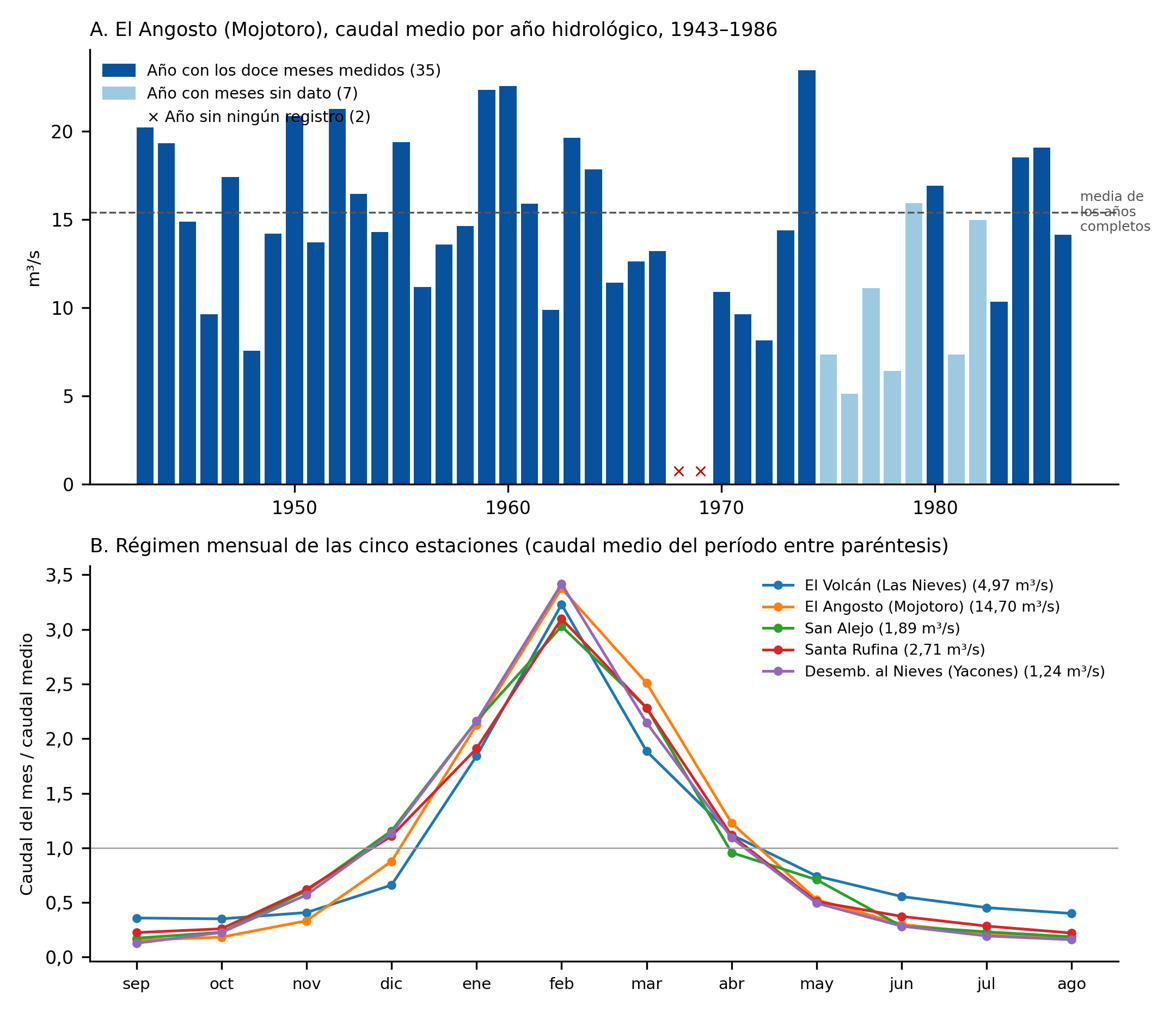
\includegraphics[width=\textwidth]{fig-caudales.png}
\caption[Caudales de la cuenca del río La Caldera, 1942--1986]{\textbf{Caudales de la cuenca, 1942--1986.} A: caudal medio de El Angosto por año hidrológico; en azul claro, los años con meses sin dato; las cruces marcan los dos años sin ningún registro. B: régimen mensual de las cinco estaciones, expresado como cociente entre el caudal de cada mes y el caudal medio del período. Elaboración propia con datos del SNIH, con las fechas corregidas.}\label{fig:caudales}
\end{figure}

\begin{ficha}{El Angosto, estación 625: qué hay dentro de los cuarenta y cuatro años}
\begin{itemize}[leftmargin=*,nosep]
\item \textbf{Faltan cuarenta y cuatro meses} de los quinientos veintiocho del período. Se concentran en dos tramos: 1967--1969, con veinticuatro meses sin dato, y 1975--1982, con veinte.
\item \textbf{Treinta y cinco de los cuarenta y cuatro años hidrológicos}, de septiembre a agosto, tienen los doce meses completos.
\item \textbf{Un defecto de la exportación, no de la serie.} Siete registros vienen fechados a las 23 horas del último día del mes anterior ---por ejemplo, el 28 de febrero de 1946--- y parecen, a primera vista, meses duplicados junto a meses faltantes. Corregida esa hora de desfase, cada valor cae en su mes y no queda ningún duplicado. El mismo defecto afecta un registro de San Alejo y otro de Santa Rufina. Los valores de este capítulo usan las fechas corregidas.
\item \textbf{Año más seco completo, 1948}, con 7,57~m³/s de media; \textbf{el más húmedo, 1974}, con 23,46, el mismo del máximo mensual de la serie.
\end{itemize}
\end{ficha}

Tres cosas se siguen de las planillas. La primera es que el dato no sólo existió: \textbf{está hoy a un clic, en una base pública del Estado nacional}, con fecha, variable y unidad. La segunda es que la serie más larga está más lejos del umbral legal de lo que su calendario sugiere: cuarenta y cuatro años de extensión, pero treinta y cinco completos. La tercera es que las series dicen algo sobre el río que ningún acto de este libro menciona. El régimen es estival y extremo: el caudal medio de febrero multiplica el de septiembre por nueve en El Volcán, por catorce en Santa Rufina, por diecisiete en San Alejo, por veintidós en El Angosto y por veintisiete en el Yacones. Y un solo mes llegó a promediar más de dieciséis metros cúbicos por segundo en cuencas de treinta y ocho y ochenta y cinco kilómetros cuadrados. Es el comportamiento que el Decreto 1.989/02 manda considerar, y que una determinación por método geomorfológico sólo puede inferir.

\textbf{Y cuarta: esa procedencia consta al pie de dos páginas de tablas, y en ningún otro
lado.} No figura en el capítulo de recopilación de antecedentes, que enumera nueve organismos
consultados sin decir qué aportó cada uno, ni en el de fuentes de información del sistema de
información geográfica, que lista doce fuentes y no menciona ninguna de las dos.

Es, en un documento técnico y en miniatura, exactamente lo que este libro llama la segunda
tesis: \textbf{el dato no está negado ni oculto; está en el lugar donde nadie lo busca.}

\begin{cautela}
Lo que este libro corrige es su propia afirmación. \textbf{No es cierto que nunca se hayan
aforado estos ríos}: se los aforó durante décadas, los registros se publicaron y siguen
disponibles.

Lo que sigue siendo cierto, y ahora se entiende mejor, es que el artículo 8 del Decreto
1.989/02 exige cincuenta años de serie y la mejor de estas estaciones abarca cuarenta y cuatro, con treinta y cinco completos, y cerró en 1986. \textbf{La determinación de línea de ribera se resuelve por método
geomorfológico no porque falte el dato, sino porque el dato que hay no alcanza el umbral que
la propia norma fijó} --- y no alcanza porque las estaciones cerraron.

Este libro descargó las cinco series, pero no verificó si alguna de las determinaciones que analiza las consultó. Ninguna las menciona. Tampoco procesó las series más allá de los valores que consigna la ficha: calcular caudales de crecida con períodos de retorno exige los caudales máximos instantáneos, no los medios mensuales, y eso es trabajo de un hidrólogo.
\end{cautela}

\subsection*{Y una sigue midiendo, treinta kilómetros aguas abajo}

La consulta del catálogo público de estaciones del Sistema de Información Hidrológica ---
mil novecientas treinta y siete estaciones de la Argentina --- permite precisar qué queda hoy
de esa red.

\textbf{De las cinco estaciones de aforo de la cuenca, ninguna figura en el catálogo activo.}
El Volcán, San Alejo, Santa Rufina y Desembocadura al Nieves no aparecen con ningún nombre ni
sobre ningún río. Tampoco hay estación alguna llamada La Caldera, Wierna, Vaqueros o Yacones.

\textbf{Pero el río Mojotoro sí tiene medición, y doble.}

\needspace{6\baselineskip}
{\small
\begin{longtable}{@{}p{3.6cm}p{2.4cm}p{2.6cm}p{3.4cm}@{}}
\toprule
\textbf{Estación} & \textbf{Tipo} & \textbf{Red} & \textbf{Registro} \\
\midrule
\endhead
Mojotoro -- Güemes & hidrológica & \mbox{Red Hidrológica} \mbox{Nacional, SSRH} & manual, base BDHI \\
Mojotoro -- Güemes & combinada & RHN -- SAT & \textbf{automática} \\
\bottomrule
\end{longtable}
}

Están a unos treinta y dos y treinta y seis kilómetros de La Caldera, ya en el departamento
General Güemes, aguas abajo de la confluencia. Una registra altura de forma manual y vuelca a
la base hidrológica nacional; la otra es \textbf{automática y forma parte del sistema de
alerta}.

Tres consecuencias, y la última corrige el reproche que este libro venía haciendo.

\textbf{Primera: la capacidad técnica existe y está desplegada en la región.} Dentro de un
radio de sesenta kilómetros hay \textbf{treinta y dos estaciones} de al menos cuatro redes
distintas --- la hidrológica nacional, el sistema de alerta, la del INTA y redes
meteorológicas ---, la mayoría automáticas. No falta equipamiento ni institución: falta
dentro de esta cuenca.

\textbf{Segunda: lo que se mide es el río después, no el río que inunda.} El Mojotoro en
Güemes recoge el aporte de toda la cuenca alta, incluido el La Caldera. Sirve para saber qué
bajó; no sirve para avisarle a La Caldera que algo está bajando, porque para cuando el agua
llega a Güemes ya pasó por el pueblo.

Es exactamente la distinción que el Plan de Manejo hace al proponer su sistema de alerta:
el punto útil está \textbf{cinco kilómetros aguas arriba} del pueblo, porque de ahí la
crecida tarda entre cuarenta y cinco y sesenta minutos en llegar. \textbf{Medir treinta
kilómetros aguas abajo es medir demasiado tarde.}

\textbf{Y tercera: el río de este departamento nunca dejó de estar medido del todo.} Lo que se
abandonó fue la medición \textit{dentro} de la cuenca. La estación de El Angosto, sobre el
mismo Mojotoro, funcionó de 1942 a 1986; hoy hay dos estaciones sobre ese río, más abajo, una
de ellas automática.

\begin{cautela}
El catálogo consultado publica la existencia y la ubicación de cada estación, no sus series.
Este libro \textbf{no consultó los registros} de las dos estaciones del Mojotoro, ni sabe
desde cuándo operan ni qué continuidad tienen.

Tampoco puede afirmar que esos datos sirvan para determinar una línea de ribera en La Caldera:
el área de aporte es distinta y el punto de medición está fuera del departamento. Lo que
registra es más modesto y más incómodo: \textbf{el Estado sigue midiendo este sistema hídrico,
sólo que en el tramo donde el agua ya no es problema de nadie de este departamento.}
\end{cautela}

\section{El procedimiento, leído}

Los veinticinco actos que este capítulo analiza invocan todos la misma norma ---varios edictos, con el número mal escrito: «1898/02»---: el \textbf{Decreto
Nº 1.989/02}, que aprueba la Resolución 070/02 de la Agencia de Recursos Hídricos y reglamenta
el artículo 126 del Código de Aguas. Hasta ahora este libro la conocía sólo por lo que decían
los actos que la citaban. Conviene leerla, porque contesta preguntas que el capítulo venía
dejando abiertas.

\textbf{Y conviene empezar por cómo se publicó}, porque la forma de la publicación dice tanto
como el contenido.

\begin{ficha}{Boletín Oficial Nº 16.515, 11 de noviembre de 2002, pág.\ 4.773}
Sección Administrativa, Decretos. La entrada del sumario reza: «\textsc{m.p.e.\ n\textup{º} 1.989 del
28/10/02 --- Código de Aguas de la Provincia de Salta, Ley N\textup{º} 7.017: art.\ 126, determinación
Líneas de Rivera}».

El cuerpo de la sección trae, bajo el título \textbf{DECRETO Nº 1.989}, un solo párrafo:

\begin{quote}
«El texto del Decreto Nº 1989/02 que reglamenta el art.\ 126 de la Ley Nº 7017 --- Código de
Aguas de Salta, \textbf{se publica como Separata de este Boletín Oficial}.»
\end{quote}

Y debajo, la fecha: \textbf{Salta, 28 de octubre de 2002}. Nada más.
\end{ficha}

\begin{cautela}
Dos cosas.

\textbf{Primera, las fechas y la edición.} El decreto es del \textbf{28 de octubre de 2002}; el 11 de noviembre es la fecha de la edición que lo publica, el \textbf{Boletín Oficial Nº 16.515}, página 4.773.

\textbf{Y segunda:} la edición del Boletín \textbf{no contiene el decreto}. Contiene una línea
que dice dónde está. El acto se publica; el texto que permitiría cumplirlo, verificarlo o
discutirlo va a un impreso aparte, que se distribuye aparte y que no forma parte del archivo
digitalizado de la edición.

\textbf{Es la estructura que el capítulo \ref{cap:opacidad} describe, en su forma más concentrada y once años antes de la serie de determinaciones que este capítulo reconstruye.} Nada de esto
es irregular: la separata es un instrumento previsto y legítimo. Lo que se registra es el
efecto. La norma que rige los veinticinco actos de línea de ribera de este departamento --- la que fija quién integra la comisión, con qué series de aforo, con qué
publicación y a costa de quién --- \textbf{no está donde dice el acto que la publica}.
\end{cautela}

\begin{ficha}{Decreto Nº 1.989/02 --- Anexo I, procedimiento en doce artículos}
\textbf{Art.\ 1º} El trámite se inicia \textbf{de oficio o a pedido de parte}.
\textbf{Art.\ 3º} La Comisión Técnica se integra con un \textbf{ingeniero hidráulico o civil,
un geólogo y un agrimensor}.
\textbf{Art.\ 4º} Notificación y \textbf{publicación por dos días} en el Boletín Oficial y en
el diario de mayor difusión.
\textbf{Art.\ 5º} Quince días para que las partes presenten información.
\textbf{Art.\ 7º} La delimitación se hace por el caudal de la \textbf{máxima crecida
ordinaria}, considerando la \textbf{migración lateral por erosión natural}.
\textbf{Art.\ 8º} Prelación de fuentes: \textbf{aforos sistemáticos con series no menores de
cincuenta años}; en su defecto, registros fotográficos y satelitales; y recién después,
modelos matemáticos de cuenca.
\textbf{Art.\ 9º} Trabajo de campo: \textbf{amojonar} a izquierda y derecha los lugares de las
más altas aguas por donde naturalmente el río ha pasado.
\textbf{Art.\ 10} La Comisión propone, la Autoridad notifica, los interesados tienen diez días
para observar, la Autoridad resuelve en diez días hábiles, \textbf{se registra en el libro de
Catastros y se comunica a la Dirección de Inmuebles, previa publicación por dos días}. El acto
es apelable ante el \textbf{Tribunal de Aguas}.
\textbf{Art.\ 11} \textbf{Los costos los absorbe quien solicita} la determinación.
\end{ficha}

Cinco cosas quedan establecidas, y tres de ellas cambian lo que este capítulo podía afirmar.

\textbf{Primera: la publicación es obligatoria y es parte del acto.} El artículo 10 no dice
que se publique el resultado: dice que la resolución «se registra en el libro de Catastros y
se comunica a la Dirección de Inmuebles, \textbf{previa publicación por dos días}». La
publicación es condición del registro, no un trámite posterior.

\begin{cautela}
El decreto \textbf{no dice expresamente que deban publicarse las coordenadas}. Dice que debe
publicarse la resolución, y que el trabajo de campo consiste en amojonar los puntos de
ribera. Este libro \textbf{no puede afirmar}, entonces, que las tres resoluciones que
remitieron sus coordenadas a la sede del organismo hayan incumplido el decreto.

Lo que sí puede afirmar es que \textbf{doce de las quince determinaciones de
2013--2015 publicaron sus coordenadas y tres no}, bajo la misma norma y en el mismo período, y las tres con el mismo asesor legal firmante. Y que las dos de esas tres que se refieren a un inmueble recaen sobre suelo que este libro
encontró en proceso de loteo ---condición que comparten, sin embargo, otras dos que sí las publicaron---. La norma admite las dos prácticas; lo que no explica es por qué
se eligió una u otra en cada caso, y eso es exactamente lo que la segunda tesis sostiene.
\end{cautela}

\textbf{Segunda: los aforos están en primer lugar de prelación, y con series de cincuenta
años.} El artículo 8 los pone antes que cualquier otro método. El capítulo \ref{cap:siglo} documenta que en 1924 el propio Estado dejó constancia escrita de no haber aforado ningún río de la provincia.
\textbf{La norma exige series de cincuenta años, y la más larga de las cinco estaciones de la cuenca ---El Angosto, 1942 a 1986--- abarca cuarenta y cuatro, de los que treinta y cinco tienen los doce meses medidos; las otras cuatro cerraron entre 1955 y 1961 con once a catorce años de registro completo.}

\textbf{Tercera: el decreto contempla que el río se mueva.} El artículo 7 manda considerar la
«migración lateral por erosión natural». Es la misma constatación que en 1940 obligó a
suspender una obra porque «el río desvió su curso», ahora incorporada al procedimiento.

\textbf{Cuarta: el acto es apelable ante el Tribunal de Aguas.} Existe una vía de revisión
específica. Este libro no encontró ningún caso del departamento que la haya usado.

\textbf{Y quinta: los costos los paga quien solicita.} Cuando el trámite lo inicia un
propietario que quiere lotear, es él quien financia la determinación de hasta dónde puede
lotear. La norma lo dice sin rodeos, y no es una anomalía: es el régimen. Pero conviene
leerlo junto al artículo 1, que permite iniciar \textbf{de oficio}: \textbf{el Estado puede
determinar la línea de ribera sin que nadie se lo pida y a su propio costo}, y este libro no
encontró constancia de que lo haya hecho en este departamento.

\section{La determinación es anterior al aluvión}

Hay un antecedente administrativo anterior a todo lo demás, y es el más incómodo del expediente.

\begin{ficha}{Boletín Oficial Nº 19.467 (2015) --- sección Determinación de Línea de Ribera}
\begin{itemize}[leftmargin=*,nosep]
\item \textbf{Orden de publicación:} 100045883, página 407.
\item \textbf{Organismo:} Secretaría de Recursos Hídricos.
\item \textbf{Expediente:} Nº \textbf{34-167.127/13}.
\item \textbf{Objeto:} \textbf{Arroyos El Durazno y Guaranguay}, inmueble \textbf{catastro Nº 4.366}, departamento La Caldera.
\end{itemize}
\end{ficha}

El cuerpo del edicto fue obtenido. Su texto establece lo siguiente:

\begin{ficha}{Edicto --- Resolución Nº 383 del 18/12/2014}
La Secretaría de Recursos Hídricos hace saber que \textbf{por Resolución Nº 383 del 18 de diciembre de 2014 se aprobó la determinación de la línea de ribera} realizada por la Comisión Técnica \textbf{en ambas márgenes de los arroyos El Durazno y Guaranguay}, en la zona del inmueble identificado con la matrícula catastral Nº 4.366 del departamento La Caldera.

Las coordenadas Posgar de las líneas de ribera determinadas \textbf{``se encuentran a disposición de los interesados en la sede de la Secretaría''}.

El acto es apelable ante el \textbf{Tribunal de Aguas} --- Decreto Nº 1898/02, art.\ 10 --- dentro de los diez días hábiles administrativos contados desde la última publicación, presentando el recurso en Avenida Bolivia 4650. Publicado los días 21 y 22 de enero de 2015 en los \textbf{Boletines Oficiales Nº 19.466 y 19.467}, orden de publicación 100045883. Salta, 20 de enero de 2015. Suscribe el edicto el Dr.\ Matías J.\ Brogin\index{Brogin, Matías J.}, asesor legal.
\end{ficha}

\begin{cautela}
No es un trámite iniciado ni pendiente: \textbf{es una determinación aprobada}. El Estado provincial fijó, por resolución firme, dónde estaba el límite del cauce en ambas márgenes de los dos arroyos.
\end{cautela}

Y la fecha es exacta hasta el punto de resultar incómoda de escribir. La resolución que aprueba la línea de ribera es del \textbf{18 de diciembre de 2014}. El primer aluvión que destruyó los loteos fue el \textbf{21 de diciembre de 2018}.

\textbf{Cuatro años y tres días.}

\begin{cautela}
El edicto agrega, además, uno de los casos del patrón que el capítulo \ref{cap:opacidad} documenta.

Lo que se publica es que la línea existe. \textbf{Dónde está} --- las coordenadas Posgar que la definen --- no se publica: queda a disposición de los interesados en la sede de la Secretaría, en avenida Bolivia 4650, primer piso, ciudad de Salta.

De modo que el acto por el cual el Estado determina hasta dónde llega el cauce de un arroyo, y por lo tanto dónde no se puede construir, se comunica sin el dato que lo hace aplicable. Un comprador de lote en El Durazno podía leer ese edicto en enero de 2015 y no saber si su parcela estaba dentro o fuera de la línea.

Corresponde señalar que el mismo Boletín publica, para otro expediente de la misma sección, la tabla completa de coordenadas. Es decir: la práctica de publicarlas existía. En este caso no se aplicó.
\end{cautela}

\begin{cautela}
Subsiste el límite ya señalado y ahora es más preciso. El inmueble es la \textbf{matrícula catastral Nº 4.366}; el loteo El Durazno se asienta sobre la \textbf{matrícula Nº 6.558}. Este libro no establece la relación entre ambas.

Lo que puede afirmarse sin ese dato es: la línea de ribera de ambas márgenes de los arroyos El Durazno y Guaranguay estaba determinada por resolución desde diciembre de 2014, y el arroyo Guaranguay es aquél cuya crecida la sentencia identifica como causa del aluvión, aquél que en enero de 2026 volvió a aislar a los barrios del sur, y aquél sobre el cual se construyó el badén de ciento veinte millones de pesos.
\end{cautela}

\section{El procedimiento, y la fuente que lo describe}

El material que este capítulo venía usando con reservas quedó identificado. Se trata de una presentación institucional titulada \textit{Línea de Ribera y Ordenamiento Territorial}, cuyo autor es el \textbf{geólogo Jorge G.\ Torres\index{Torres, Jorge G.}, de la Secretaría de Recursos Hídricos de Salta}, publicada por el \textbf{Consejo Hídrico Federal (COHIFE)}. La reserva se levanta: es un documento oficial, de autor identificable, y su autor figura en diciembre de 2025 como \textbf{Director General de Cuencas y Política Hídrica} de la Subsecretaría --- es decir, el funcionario a cargo del área donde vive el Plan de Manejo de esta causa.

\begin{cautela}
La presentación agrega un dato que reordena el capítulo entero.

\begin{quote}
``La Secretaría de Recursos Hídricos, en el área de Infraestructura Hídrica, es la que emite el \textbf{Certificado de No Inundabilidad}. Trámite necesario para loteos o urbanizaciones, que algunos de los límites sea un río, se exige en primera medida la determinación de la línea de ribera, además de otros requisitos.''
\end{quote}

El loteo El Durazno está atravesado por los arroyos El Durazno y Guaranguay, cuya línea de ribera se determinó en 2014. El organismo que la determinó es el mismo que emite el Certificado de No Inundabilidad, y ese organismo intervino \textbf{a fojas 59} del expediente de aprobación del plano.

\textbf{La pregunta del capítulo deja de ser abierta y pasa a tener una única forma: ¿se emitió Certificado de No Inundabilidad para El Durazno, y en qué términos?} Si la foja 59 lo contiene, hay que leerlo. Si no lo contiene, hay que preguntar por qué un fraccionamiento limitado por dos cursos de agua se aprobó sin él. Este libro no sabe la respuesta y no la insinúa; señala que la pregunta ahora es contestable con una sola foja.
\end{cautela}

Y un segundo dato, sobre el visado. La presentación describe que, obtenida la resolución, ``el interesado puede realizar el plano y la Secretaría de Recursos Hídricos visa el mismo'', y enumera los requisitos: que los puntos de vinculación estén graficados, que las planillas lleven las coordenadas, y \textbf{que se mencione el número de Resolución}.

Eso vuelve verificable algo que hasta aquí no lo era. Si el plano 1.164 fue visado por Recursos Hídricos, debe mencionar en su carátula el número de la resolución de línea de ribera. \textbf{Basta mirar el plano para saber si la línea de 2014 fue incorporada al fraccionamiento de 2021.} Es una comprobación de un minuto, sobre un documento que ya está identificado.

\section{Lo que la Provincia ya hacía en 2012 y 2013}

Tres edictos anteriores a la serie muestran que las formas que después variaron ya estaban todas disponibles.

\begin{ficha}{Resolución Nº 94/12 --- B.O.\ Nº 19.130 y 19.131, 22 y 23 de agosto de 2013}
Expediente 0050034-71745/2011. Dictada el 2 de mayo de 2012; publicada quince meses después, con la transcripción literal de su parte dispositiva. Tiene por conformada la comisión técnica y determina la línea de ribera del \textbf{río Castellanos}, ambas márgenes, en la \textbf{matrícula 4027}, «cuya gráfica ilustra plano que forma parte del informe», con dos vértices por margen en coordenadas publicadas.

\textbf{Art.\ 3º:} advierte al propietario que, «\textbf{dada la peligrosidad del Río Castellanos}, que en oportunidad de crecidas extraordinarias podría rebasar eventualmente la línea de ribera demarcada, \textbf{deberá evitar la construcción de viviendas en la proximidad de la ribera}».

\textbf{Art.\ 4º:} la publicación es previa al registro de la línea «en el Libro de Catastros de la Secretaría de Recursos Hídricos» (art.\ 10 de la Resolución 070/02).

\textbf{Art.\ 5º:} comunica la resolución al Ministerio, al propietario, al ingeniero en construcciones Pablo Vicente Balverdi y \textbf{a la Dirección General de Inmuebles}. Firman el secretario Fuertes y la jefa del Programa Fiscalización y Control, Silvia F.\ Santamaría.
\end{ficha}

\begin{ficha}{Resolución Nº 155 del 05/06/2013 --- B.O.\ Nº 19.093, 28 de junio y 1 de julio de 2013}
Expediente 34-132.589/12. Determina la línea de ribera del \textbf{arroyo Los Nogales} en la \textbf{matrícula 1905}, sección A, fracción 17b ---el inmueble de la futura urbanización Cerro de Buena Vista---. «Las coordenadas de vinculación determinadas \textbf{se encuentran a disposición de los terceros interesados por mesa de entradas}.» Cita el artículo 126 del Código de Aguas y el Decreto 1989/02 con su número correcto. Firma Brogin.
\end{ficha}

\begin{ficha}{Resolución Nº 201 del 01/07/2013 --- B.O.\ Nº 19.109 y 19.110, 23 y 24 de julio de 2013}
Expediente 34-214.573/12. Determina la línea de ribera del \textbf{río Vaqueros}, ambas márgenes, en el inmueble de «matrícula catastral \textbf{S/Nº}», sección B, localidad de Vaqueros. \textbf{Publica dieciocho coordenadas Posgar}: trece en la margen izquierda y cinco en la derecha, a lo largo de unos trescientos sesenta metros. Cita el «Dcto.\ 1898/02». Firma Brogin.
\end{ficha}

\begin{cautela}
Tres observaciones, de peso desigual.

\textbf{La primera es la que más pesa.} En mayo de 2012 la Secretaría de Recursos Hídricos no se limitó a fijar una línea: advirtió por escrito al propietario que no construyera viviendas cerca de la ribera de un río peligroso, aunque la línea quedara demarcada, y comunicó la resolución a Inmuebles, el organismo que aprueba los planos. El instrumento para prevenir, en el mismo acto que fija la ribera, existía y se usaba dos años antes de la determinación de El Durazno. Este libro no encontró una advertencia equivalente en ningún acto sobre los arroyos El Durazno y Guaranguay; el edicto de la Resolución 383/14 no la trae, aunque, como se dijo, un edicto es sólo la síntesis de la resolución.

\textbf{La segunda es de forma.} Los tres edictos, del mismo año de publicación y con el mismo asesor en dos de ellos, muestran las tres variantes que la serie posterior alterna: coordenadas publicadas (201/13), coordenadas en mesa de entradas (155/13) y parte dispositiva transcripta con advertencias (94/12). También muestran que la cita equivocada del decreto convivía, en 2013, con la correcta. Una curiosidad de la 94/12: sus dos vértices de la margen izquierda distan entre sí cinco metros; los de la derecha, casi doscientos.

\textbf{La tercera es de lugar.} La línea del río Vaqueros de 2013 termina, en uno de sus extremos, a trece metros del primer punto de la ampliación que la Resolución 144/17 agregó en 2017 a la línea de la matrícula 40. Leídas juntas, las Resoluciones 201/13, 414/16 y 144/17 fijan más de seiscientos metros continuos del mismo río, con un ancho entre márgenes de cien a ciento cuarenta metros, en tres actos y cuatro años, para inmuebles vecinos. El de 2013 no tenía número de matrícula. Y ese tramo del río es límite departamental: según la cartografía de radios del Censo 2022, el punto medio entre ambas márgenes cae a seis metros (2013) y a trece (2016) del límite de La Caldera, del lado del departamento Capital. Las líneas de las dos orillas se fijaron en expedientes de La Caldera, aunque la margen derecha está, para el INDEC, en otro departamento. \pendiente{identificación del inmueble «s/Nº» de la sección B de Vaqueros y su relación con la matrícula 40}
\end{cautela}

\section{Dos años, veinticinco actos}

La determinación de diciembre de 2014 sobre El Durazno y Guaranguay no fue un acto aislado. Entre octubre de 2013 y diciembre de 2015 la Secretaría de Recursos Hídricos dictó veinticinco actos de comisión o de determinación sobre la cuenca del río La Caldera y sus afluentes; la tabla agrega la Resolución 023/14, que designa y determina a la vez.

\textbf{Conviene fijar la base del recuento, porque este capítulo la usa de dos maneras.} La tabla tiene veintiséis filas: \textbf{diez comisiones}, \textbf{quince determinaciones} ---incluida la 023/14, que la serie cuenta aparte por designar y determinar en un solo acto--- y una fila del índice del Boletín cuyo acto no se identificó. Cuando este libro dice «veinticinco actos» excluye a la 023/14; cuando dice «quince determinaciones» la incluye. Son dos recuentos distintos de la misma tabla y ninguno contiene al otro.

\needspace{6\baselineskip}
{\sffamily\bfseries\footnotesize Actos de línea de ribera en el departamento, octubre de 2013 -- diciembre de 2015 \textit{(por fecha de publicación; la columna consigna la fecha de dictado, y por eso la primera fila es de julio de 2013. Dos filas rompen ese orden a propósito: la Resolución 428/15, cuyo edicto salió en febrero de 2016, y la Resolución 383/14, que se deja al final por ser el acto que este capítulo persigue)}\par}
\vspace{0.5em}
{\small
\setlength{\LTpre}{0.6em}\setlength{\LTpost}{1.2em}
\begin{longtable}{@{}p{2.2cm}p{2.9cm}p{6.8cm}@{}}
\toprule
\textbf{Acto} & \textbf{Expediente} & \textbf{Objeto} \\
\midrule
\endhead
Res.\ 208/13 (22/07/13) & 34-240.329/12 & \textbf{Comisión}: arroyo Quintín o Pacará, catastro 3989, fracción 78. Integran el ing.\ civil César Soto, el geólogo Marcelo Ramón Olañeta y el técnico Félix Márquez. B.O.\ 20 y 21/11/2013 \\
Res.\ 292/13 (10/10/13) & 34-160.869/13 & \textbf{Comisión}: arroyo Quintín, catastro 3756, fracción 48. B.O.\ 27 y 28/03/2014. La determinación llega en 2025 (Res.\ 142/2025) \\
Res.\ 348/13 (19/11/13) & --- & \textbf{Determinación}: río La Caldera, matrícula 1590, La Calderilla. \textit{Con coordenadas y zona inundable publicadas} \\
Res.\ 395/13 (26/12/13) & 34-167.127/13 & \textbf{Comisión}: río La Caldera y arroyo del Manzano, catastro 4366 (el aviso dice «1366»), Finca La Caldera o Getsemaní \\
Res.\ 6/14 (13/01/14) & 34-179.209/12 & \textbf{Determinación}: río La Caldera, matrícula 3593, fracción 17. \textit{Con coordenadas publicadas} \\
Res.\ 7/14 (13/01/14) & 34-19.384/12 & \textbf{Determinación}: río La Caldera, matrícula 3584, La Calderilla. \textit{Con coordenadas publicadas} \\
Res.\ 8/14 (13/01/14) & 34-207.589/12 & \textbf{Comisión}: quebrada de la matrícula 4191, Fracción Finca Vaqueros \\
Res.\ 023/14 (06/02/14) & 90.034-96.837/13 & Designa al geólogo Jorge G.\ Torres\index{Torres, Jorge G.} y \textbf{determina} la línea de ribera del río La Caldera a lo largo del \textit{pueblo}; coordenadas en el anexo vinculado \\
Res.\ 80/14 (07/04/14) & 34-240.329/12 & \textbf{Determinación}: arroyo Quintín o Pacará, matrícula 3989, fracción 78, Finca Vaqueros --- \textit{el inmueble del Club de Campo Las Vertientes}. \textit{Con coordenadas publicadas} \\
Res.\ 96/14 (29/04/14) & 34-61.721/14 & \textbf{Comisión}: río Vaqueros, catastros 1905 sec.\ A frac.\ 17-b y 3740 frac.\ 47 \\
Res.\ 101/14 (29/04/14) & 34-207.589/12 & \textbf{Determinación}: arroyo Los Nogales Norte o El Cajón, matrícula 4191. \textit{Con coordenadas publicadas} \\
Res.\ 182/14 (03/07/14) & 34-160.829/13 & \textbf{Determinación}: río La Caldera, matrícula 2882, fracciones 1 y 3, La Calderilla. \textit{Con coordenadas publicadas} \\
\textbf{Res.\ 185/14} (11/07/14) & \textbf{34-167.127/13} & \textbf{Determinación}: río La Caldera y arroyo El Manzano, \textbf{matrícula 4366}, Finca La Caldera o Getsemaní. \textit{Con coordenadas publicadas} \\
Res.\ 142/14 (27/05/14) & 125-19.223/09 & \textbf{Determinación}: ríos Mojotoro y La Caldera, matrícula 3616 ---el inmueble del loteo La Misión Etapa III---. \textit{Sin coordenadas publicadas} \\
Res.\ 209/14 (29/07/14) & 34-61.721/14 & \textbf{Determinación}: río Vaqueros, matrículas 1905 y 3740. \textit{Con coordenadas publicadas} \\
Res.\ 74/15 (10/03/15) & 34-259.760/14 & \textbf{Comisión}: río La Caldera, catastros 3721 y 3722, Fracción Finca Wierna \\
Res.\ 197/15 (05/06/15) & 34-284.285/14 & \textbf{Comisión}: río La Caldera, catastro 4049. Integran el \textbf{geólogo Jorge Torres} y el ing.\ civil Carlos Cerezo. Método geológico-morfológico; el índice del Boletín titula el aviso con Aguas del Norte \\
Res.\ 198/15 (05/06/15) & 34-145.043/15 & \textbf{Comisión}: río Vaqueros, catastros 156, 23, 1695 y 406 \\
--- (jul.\ 2015) & 34-485.548/14 & Arroyo Isasmendi, Finca Wierna, catastro 2020 (sólo el título del índice) \\
Res.\ 428/15 (03/12/15) & 34-\textbf{1}85.548/14 & \textbf{Determinación}: \textbf{río La Caldera}, matrícula 2020, Fracción A, Finca Wierna; el texto dice «Dpto.\ La Candelaria». \textit{Con coordenadas publicadas} (trece puntos en la margen izquierda, cuatro en la derecha). Edicto del 22/12/2015, B.O.\ 10 y 11/02/2016 \\
Res.\ 273/15 (13/08/15) & 34-125.733/15 & \textbf{Comisión}: río Trancas, catastro 4445, Fracción 195, Finca Vaqueros. Integran Forns, el geólogo Teodoro Chafatinos y el ing.\ civil Lucas Vidal. La determinación resultante (Res.\ 14/16) nombra el río Wierna \\
Res.\ 293/15 (31/08/15) & 34-259.760/14 & \textbf{Determinación}: río La Caldera y Cañada Oeste, matrículas 3721 y 3722, Finca Wierna. \textit{Con coordenadas publicadas}. Edicto del 08/09/2015, B.O.\ Nº 19.666, 18 y 19/11/2015 \\
Res.\ 322/15 (25/09/15) & 34-145.043/15 & \textbf{Determinación}: río Vaqueros, matrículas 156, 23, 1695 y 406. \textit{Con coordenadas publicadas}. El edicto cita el expediente como 34-145.043/\textbf{14}; el de la comisión 198/15, como /15. Edicto del 26/10/2015, B.O.\ Nº 19.675, 2 y 3/12/2015 \\
Res.\ 319/15 (16/09/15) & 34-171.172/15 & \textbf{Comisión}: río Wierna, matrículas 4097, 4953, 391, 389, 1268, 3718 y 3438. Integran el geólogo Jorge Torres y el ing.\ Carlos Cerezo. Edicto del 26/10/2015, publicado recién el 21 y 22/12/2015 \\
\textit{Res.\ 467/15} (04/12/15) & 34-30.704/15 & \textit{Determinación}: río Lesser, tramo entre el puente de la R.P.\ 115 y su confluencia con el río Castellanos. \textit{Sin coordenadas publicadas} \\
Res.\ 383/14 (18/12/14) & 34-167.127/13 & \textbf{Determinación}: arroyos El Durazno y Guaranguay, matrícula 4366. \textit{Sin coordenadas publicadas} \\
\bottomrule
\end{longtable}
}

Firmados por el Dr.\ Matías J.\ Brogin\index{Brogin, Matías J.}, Asesor Legal, salvo el de la Resolución 023/14, que firma el secretario Alfredo Fuertes. Los que aprueban comisiones invocan el \textbf{Decreto 1989/02, art.\ 8 ap.\ 2 y 3}, prohíben a los ribereños modificar las márgenes mientras dure la operación y abren quince días hábiles para que terceros aporten estudios.

Hay cuatro cuestiones que esta serie resuelve.

\textbf{Primera: el edicto inicial existe, y este capítulo lo tiene.} Se venía pidiendo el acto que aprueba la comisión técnica, con nombres y método, previo a la determinación. Las Resoluciones 395/13 y 8/14 son exactamente eso, publicadas con la estructura completa: integrantes, inmueble, prohibición cautelar y plazo de quince días. La pregunta ya no es si ese acto se publica: se publica. La pregunta es si se publicó \textbf{para los arroyos El Durazno y Guaranguay}, y sigue sin aparecer.

\textbf{Segunda: las comisiones no tienen composición fija, y hay un nombre que se repite.} La 292/13 nombra al ingeniero civil \textbf{Antonio Alejandro Forns\index{Forns, Antonio Alejandro}} y al geólogo Teodoro Chafatinos. La 395/13 nombra al mismo Forns y al geólogo Mario Raúl Orte. La 208/13 nombra tres: el ingeniero civil César Soto, el geólogo Marcelo Ramón Olañeta y el técnico Félix Márquez. La 8/14 nombra tres: el ingeniero civil César Manuel Soto, el geólogo Jorge David Afranllie y el técnico universitario en topología Félix Márquez. La 96/14 nombra al ingeniero Wanny Caramella y a la geóloga Marcia Jesica Faviana. La 273/15, dos años después de la 292/13, vuelve a reunir a Forns y a Chafatinos, con un tercer integrante. La del río Bermejo, en 2019, nombra dos.

El artículo 3º del Anexo I prevé ingeniero hidráulico, geólogo y agrimensor. En la práctica la integración varía entre dos y tres miembros, la especialidad del ingeniero varía, y \textbf{en ninguna de las ocho comisiones cuya integración consta aparece un agrimensor}. Entre todas las comisiones que este capítulo leyó después, de 2011 a 2019, sólo una ---la del río Vaqueros de 2016--- incluye un ingeniero hidráulico. Es un dato sobre la aplicación de la norma, no sobre su texto, y merece preguntarse a la autoridad de aplicación.

\textbf{Tercera: el departamento estaba siendo relevado sistemáticamente.} Veinticinco actos en veintiséis meses, sobre más de veinticinco inmuebles y trece cursos distintos --- los ríos La Caldera, Vaqueros, Mojotoro, Wierna, Lesser y Trancas, la Cañada Oeste, y los arroyos Quintín o Pacará, Los Nogales Norte o El Cajón, El Manzano, Isasmendi, El Durazno y Guaranguay. La línea de ribera no se fijaba de manera ocasional: \textbf{había un programa en curso}, y el departamento entero estuvo bajo relevamiento hídrico entre 2013 y 2015, con los ciclos de comisión y determinación completándose uno tras otro.

Eso vuelve muy difícil sostener que la determinación sobre los arroyos del loteo El Durazno fuera un hecho excepcional, aislado o desconocido para la administración. Y agrega una pregunta que el capítulo no tenía: \textbf{¿por qué se relevó tanto y tan seguido justo entonces?} Un programa de esa intensidad suele responder a una decisión, a un financiamiento o a un conflicto previo. Cuál de los tres es materia del expediente administrativo del programa, no de los edictos.

\begin{cautela}
\textbf{Y hay un cuarto hallazgo, que es el que más pesa: el ciclo se completa y se publica entero.}

La Resolución 8/14 de enero aprobó la comisión técnica para ``la quebrada que atraviesa la matrícula 4191'', expediente 34-207.589/12. La Resolución 101/14, del 29 de abril, aprueba la determinación resultante sobre esa misma matrícula y ese mismo expediente, y el edicto \textbf{publica las coordenadas completas}. Entre una y otra pasaron tres meses y medio. La quebrada, además, deja de ser anónima: se llama \textbf{arroyo Los Nogales Norte o El Cajón}.

El mismo ciclo se ve en el arroyo Quintín o Pacará: la Resolución 208/13, de julio de 2013, designa la comisión sobre el catastro 3989, y la 80/14, de abril de 2014, aprueba la determinación con coordenadas, ocho meses y medio después, en el mismo expediente. No todos los ciclos se cerraron tan rápido: la comisión de la Resolución 292/13 sobre el catastro 3756, publicada en marzo de 2014, recién tuvo su determinación en junio de 2025.

Con eso puede hacerse el recuento que este capítulo necesitaba. De las \textbf{once determinaciones} de línea de ribera publicadas en el departamento entre noviembre de 2013 y diciembre de 2014, más una rectificación:
\end{cautela}

{\small
\setlength{\LTpre}{0.6em}\setlength{\LTpost}{1.2em}
\begin{longtable}{@{}p{2.1cm}p{6.6cm}p{3.2cm}@{}}
\toprule
\textbf{Resolución} & \textbf{Curso e inmueble} & \textbf{Coordenadas} \\
\midrule
\endhead
348/13 & Río La Caldera, matrícula 1590 & \textbf{Publicadas} \\
6/14 & Río La Caldera, matrícula 3593 & \textbf{Publicadas} \\
7/14 & Río La Caldera, matrícula 3584 & \textbf{Publicadas} \\
023/14 & Río La Caldera, a lo largo del pueblo & \textbf{Publicadas en el anexo} \\
80/14 & Arroyo Quintín, matrícula 3989 & \textbf{Publicadas} \\
101/14 & Arroyo Los Nogales Norte, matrícula 4191 & \textbf{Publicadas} \\
\textit{142/14} & \textit{Ríos Mojotoro y La Caldera, matrícula 3616} & \textit{Remitidas a la sede} \\
\textit{236/14} & \textit{Rectifica parcialmente la 142/14} & \textit{Remitidas a la sede} \\
182/14 & Río La Caldera, matrícula 2882 & \textbf{Publicadas} \\
\textbf{185/14} & \textbf{Río La Caldera y arroyo El Manzano, matrícula 4366} & \textbf{Publicadas} \\
209/14 & Río Vaqueros, matrículas 1905 y 3740 & \textbf{Publicadas} \\
\midrule
\textbf{383/14} & \textbf{Arroyos El Durazno y Guaranguay, \textit{matrícula 4366}} & \textbf{Remitidas a la sede} \\
\bottomrule
\end{longtable}
}

\begin{cautela}
\textbf{En ese tramo, nueve de once publicaron sus coordenadas} ---con una reserva sobre el numerador: las coordenadas que se publicaron para la Resolución 6/14 y para la 7/14 son las de la línea del pueblo que después aprobó la 023/14, según se explica más abajo, y al menos las de la 7/14 no corresponden a su inmueble. Contando sólo las que publicaron las propias, la proporción es ocho de once, o siete si tampoco las de la 6/14 son suyas, y el sentido no cambia---. Las dos que no lo hicieron son la Resolución 142/14, sobre los ríos Mojotoro y La Caldera en la matrícula 3616, y la Resolución 383/14, sobre los arroyos del loteo que se inundó cuatro años después.

La 142/14, además, tuvo que ser corregida: por \textbf{Resolución 236 del 25 de agosto de 2014} la Secretaría rectificó parcialmente su artículo 1º, y avisó que ``las coordenadas correctas se encuentran a disposición de los interesados en la sede''. Una determinación con coordenadas equivocadas, rectificada sin publicar ni las erróneas ni las correctas. Los dos avisos lo confirman: el de la 142/14 salió el 13 y el 14 de agosto de 2014 ---Boletines Nº 19.363 y 19.364, orden 100042974---, dos meses y medio después de dictada la resolución; el de la 236/14, el 3 de septiembre ---Boletín Nº 19.377, orden 100043378---, por un solo día. Ninguno ofrece enlace «Ver anexo». El segundo, además, cambia de régimen de impugnación: en lugar de la apelación ante el Tribunal de Aguas invoca el artículo 309 del Código de Aguas y el Decreto 1100, y el índice del Boletín le asigna el expediente «34-19.223/09» en lugar del 125-19.223/09 de la resolución que rectifica.

\textbf{Corresponde una rectificación.} Una versión anterior de este apartado afirmaba que la 383/14 era la única de la serie sin coordenadas publicadas. \textbf{No lo es}: la 142/14, de mayo de 2014, usa exactamente la misma fórmula --- ``se encuentran a disposición de los interesados en la sede'' --- y también remite. La afirmación de unicidad era errónea y queda retirada.

Lo que subsiste, y es lo que importa, es que \textbf{la práctica dominante fue publicar}: nueve de once en 2013--2014. Las tres determinaciones de 2015 sobre la Finca Wierna ---la 293/15 y la 428/15--- y sobre el río Vaqueros ---la 322/15--- también publicaron sus coordenadas; la cuarta de ese año, la 467/15, no, y se analiza enseguida. Con ellas la serie queda en doce de quince, y la proporción se sostiene.
\end{cautela}

\begin{cautela}
Y las dos excepciones tienen algo en común.

En octubre de 2015 la Secretaría de Recursos Hídricos publicó la gestión de \textbf{El Chalchal S.R.L.}, ``co-titular registral del inmueble \textbf{Catastro Nº 3616} del Dpto.\ La Caldera'', para obtener concesión de agua subterránea destinada al \textbf{abastecimiento poblacional de 580 habitantes --- 116 lotes --- del Loteo ``La Misión Etapa III''}. La matrícula 3616 es la de la Resolución 142/14; la 4366, la de la 383/14, sobre la que se tramitaba el agua para \textbf{cuatrocientos lotes de El Durazno}.

\textbf{Las dos determinaciones de ese tramo que no publicaron coordenadas recaen sobre suelo que este relevamiento encontró en proceso de loteo.} Pero la condición no basta para explicar la diferencia: entre las nueve que publicaron hay dos que también recaen sobre suelo en loteo ---la 80/14, sobre el inmueble del club de campo Las Vertientes, y la 185/14, sobre la misma matrícula 4366---, de modo que la coincidencia es parcial y no autoriza una regla.

\textbf{Hay un tercer caso, y acota la afirmación.} La Resolución 467/15, de diciembre de 2015, aprobó la línea de ribera del \textbf{río Lesser} entre dos puntos geográficos y también remitió las coordenadas a la sede. Es un acto de otra clase ---delimita un tramo de curso y no un inmueble--- y su pertenencia al departamento es probable ---los edictos de 2009 y 2011 que este capítulo transcribe ubican los ríos Lesser y Castellanos en el departamento La Caldera---, aunque el paraje Lesser aparece en otros actos bajo jurisdicción de San Lorenzo. Por eso la distinción se formula entre determinaciones \textbf{referidas a inmuebles}.

Y hay un dato que descarta la explicación benigna. \textbf{La Resolución 185/14 recae sobre la misma matrícula 4366 que la 383/14}: mismo inmueble ---la Finca La Caldera o Getsemaní---, mismo organismo, mismo asesor legal firmante, cinco meses de diferencia. Más aún, las dos salen del mismo expediente. En julio de 2014 ese edicto ---Boletines Oficiales Nº 19.346 y 19.347, del 21 y el 22 de julio--- publicó \textbf{ciento trece pares de coordenadas} ---trazados en la lámina \ref{fig:formacionradios}--- de los otros dos cursos de la finca: veintiuno del río La Caldera, catorce en la margen derecha y siete en la izquierda, y noventa y dos del arroyo El Manzano, en dos tramos. Lo hizo con un arancel de doscientos cincuenta pesos; en diciembre, sobre El Durazno y Guaranguay, remitió las suyas a la sede. El edicto de la Resolución 348/13 había publicado once pares ---u ocho, si se cuentan sólo los de la línea; la diferencia sigue sin cotejarse--- por ciento ochenta pesos: \textbf{entre diez y catorce veces más coordenadas por un cuarenta por ciento más de arancel}. La hipótesis del costo, de la composición o de la extensión no se sostiene.

Este libro \textbf{no afirma} que la omisión haya sido deliberada, ni que alguien la decidiera para favorecer a nadie: puede ser una decisión de trámite, un criterio del profesional interviniente o un error, y con once casos las coincidencias ocurren. Lo que hace es registrar el hecho y formular la pregunta: \textbf{por qué las coordenadas de los arroyos que atraviesan el loteo El Durazno no se publicaron, cuando las de los otros dos cursos de la misma finca sí.} Se responde con los dos expedientes y con el informe técnico de sus comisiones, y ninguno está en poder de este trabajo.
\end{cautela}

\subsection*{Ocho años después, el organismo dibujó el resultado}

Todo lo anterior se reconstruyó leyendo edictos de a uno. En mayo de 2022, cumpliendo un
mandato de la sentencia que analiza el capítulo \ref{cap:amparo}, la propia Secretaría de Recursos Hídricos
puso esa serie en un mapa: la \textbf{lámina \ref{lam:mapa2}} es la ubicación de las líneas de
ribera registradas por el organismo sobre el río La Caldera y sus cauces aportantes, aguas
arriba de la confluencia con el Wierna, a escala \textbf{1:40.000} y en \textbf{POSGAR 2007,
Faja 3}.

Vale la pena mirar qué trae, además de los trazos de ribera. La misma hoja superpone los
\textbf{polígonos catastrales} clasificados en urbano, subrural y rural, y los topónimos de las
fincas que este libro viene siguiendo desde el capítulo \ref{cap:fincas}: El Durazno, Guaranguay, Finca de
Linares, El Manzano, La Calderilla, Wierna, Los Yacones. \textbf{Las líneas de ribera y las
parcelas están, por primera vez, en el mismo plano y en el mismo sistema de coordenadas.}

\lamina{lam-mapa2-ribera.jpg}{lam:mapa2}%
{Líneas de ribera registradas sobre el río La Caldera y sus afluentes, hasta 2022}%
{\textbf{Mapa Nº 2.} Ubicación de las líneas de ribera en márgenes del río La Caldera y sus
cauces aportantes, aguas arriba de la unión con el río Wierna, registradas en la Secretaría de
Recursos Hídricos hasta el año 2022. Escala 1:40.000, sistema POSGAR 2007 --- Faja 3. Sobre la
misma base, los polígonos catastrales clasificados en urbano, subrural y rural.}%
{«Informe de mapas de cuenca de río La Caldera», Secretaría de Recursos Hídricos de Salta, mayo
de 2022, presentado en la ejecución de sentencia del amparo colectivo, expediente
INC-23860/1. Reproducción facsimilar; se recortó el margen en blanco del escaneo y no se
alteraron los tonos.}

\begin{cautela}
Dos advertencias sobre el uso de esta lámina.

\textbf{No reemplaza el cotejo.} A la resolución del ejemplar incorporado al expediente puede
verse dónde hay trazos de ribera y dónde no, pero no puede establecerse con seguridad qué
resolución corresponde a cada trazo ni si el inventario gráfico coincide exactamente con los
veinticinco actos que este capítulo reconstruyó. Eso se resuelve con las capas vectoriales, que
la Secretaría no publica; la lámina \ref{fig:riberaedictos}, más abajo, reconstruye una parte
con las coordenadas que sí publicó.

\textbf{Y no cubre el departamento entero.} El mapa se detiene en la confluencia con el río
Wierna: las determinaciones sobre el río Vaqueros --- la 209/14, la 322/15 --- y los arroyos
del municipio vecino quedan fuera del recorte. La partición cartográfica repite, sin
proponérselo, la partición jurisdiccional que el capítulo \ref{cap:vaqueros} documenta.
\end{cautela}

\subsection*{Las líneas que se pueden dibujar}

Veinte resoluciones de la serie publican sus coordenadas completas: diecinueve en el cuerpo del aviso y la 023/14 en el anexo vinculado a él. Las dos que publicaron coordenadas ajenas ---la 6/14 y la 7/14--- se explican más abajo y no se dibujan. Transcriptos y llevados al mismo sistema que la capa catastral, permiten dibujar lo que el Mapa Nº~2 muestra sin identificar: qué línea corresponde a cada resolución (lámina \ref{fig:riberaedictos}).

\begin{figure}[p]
\centering
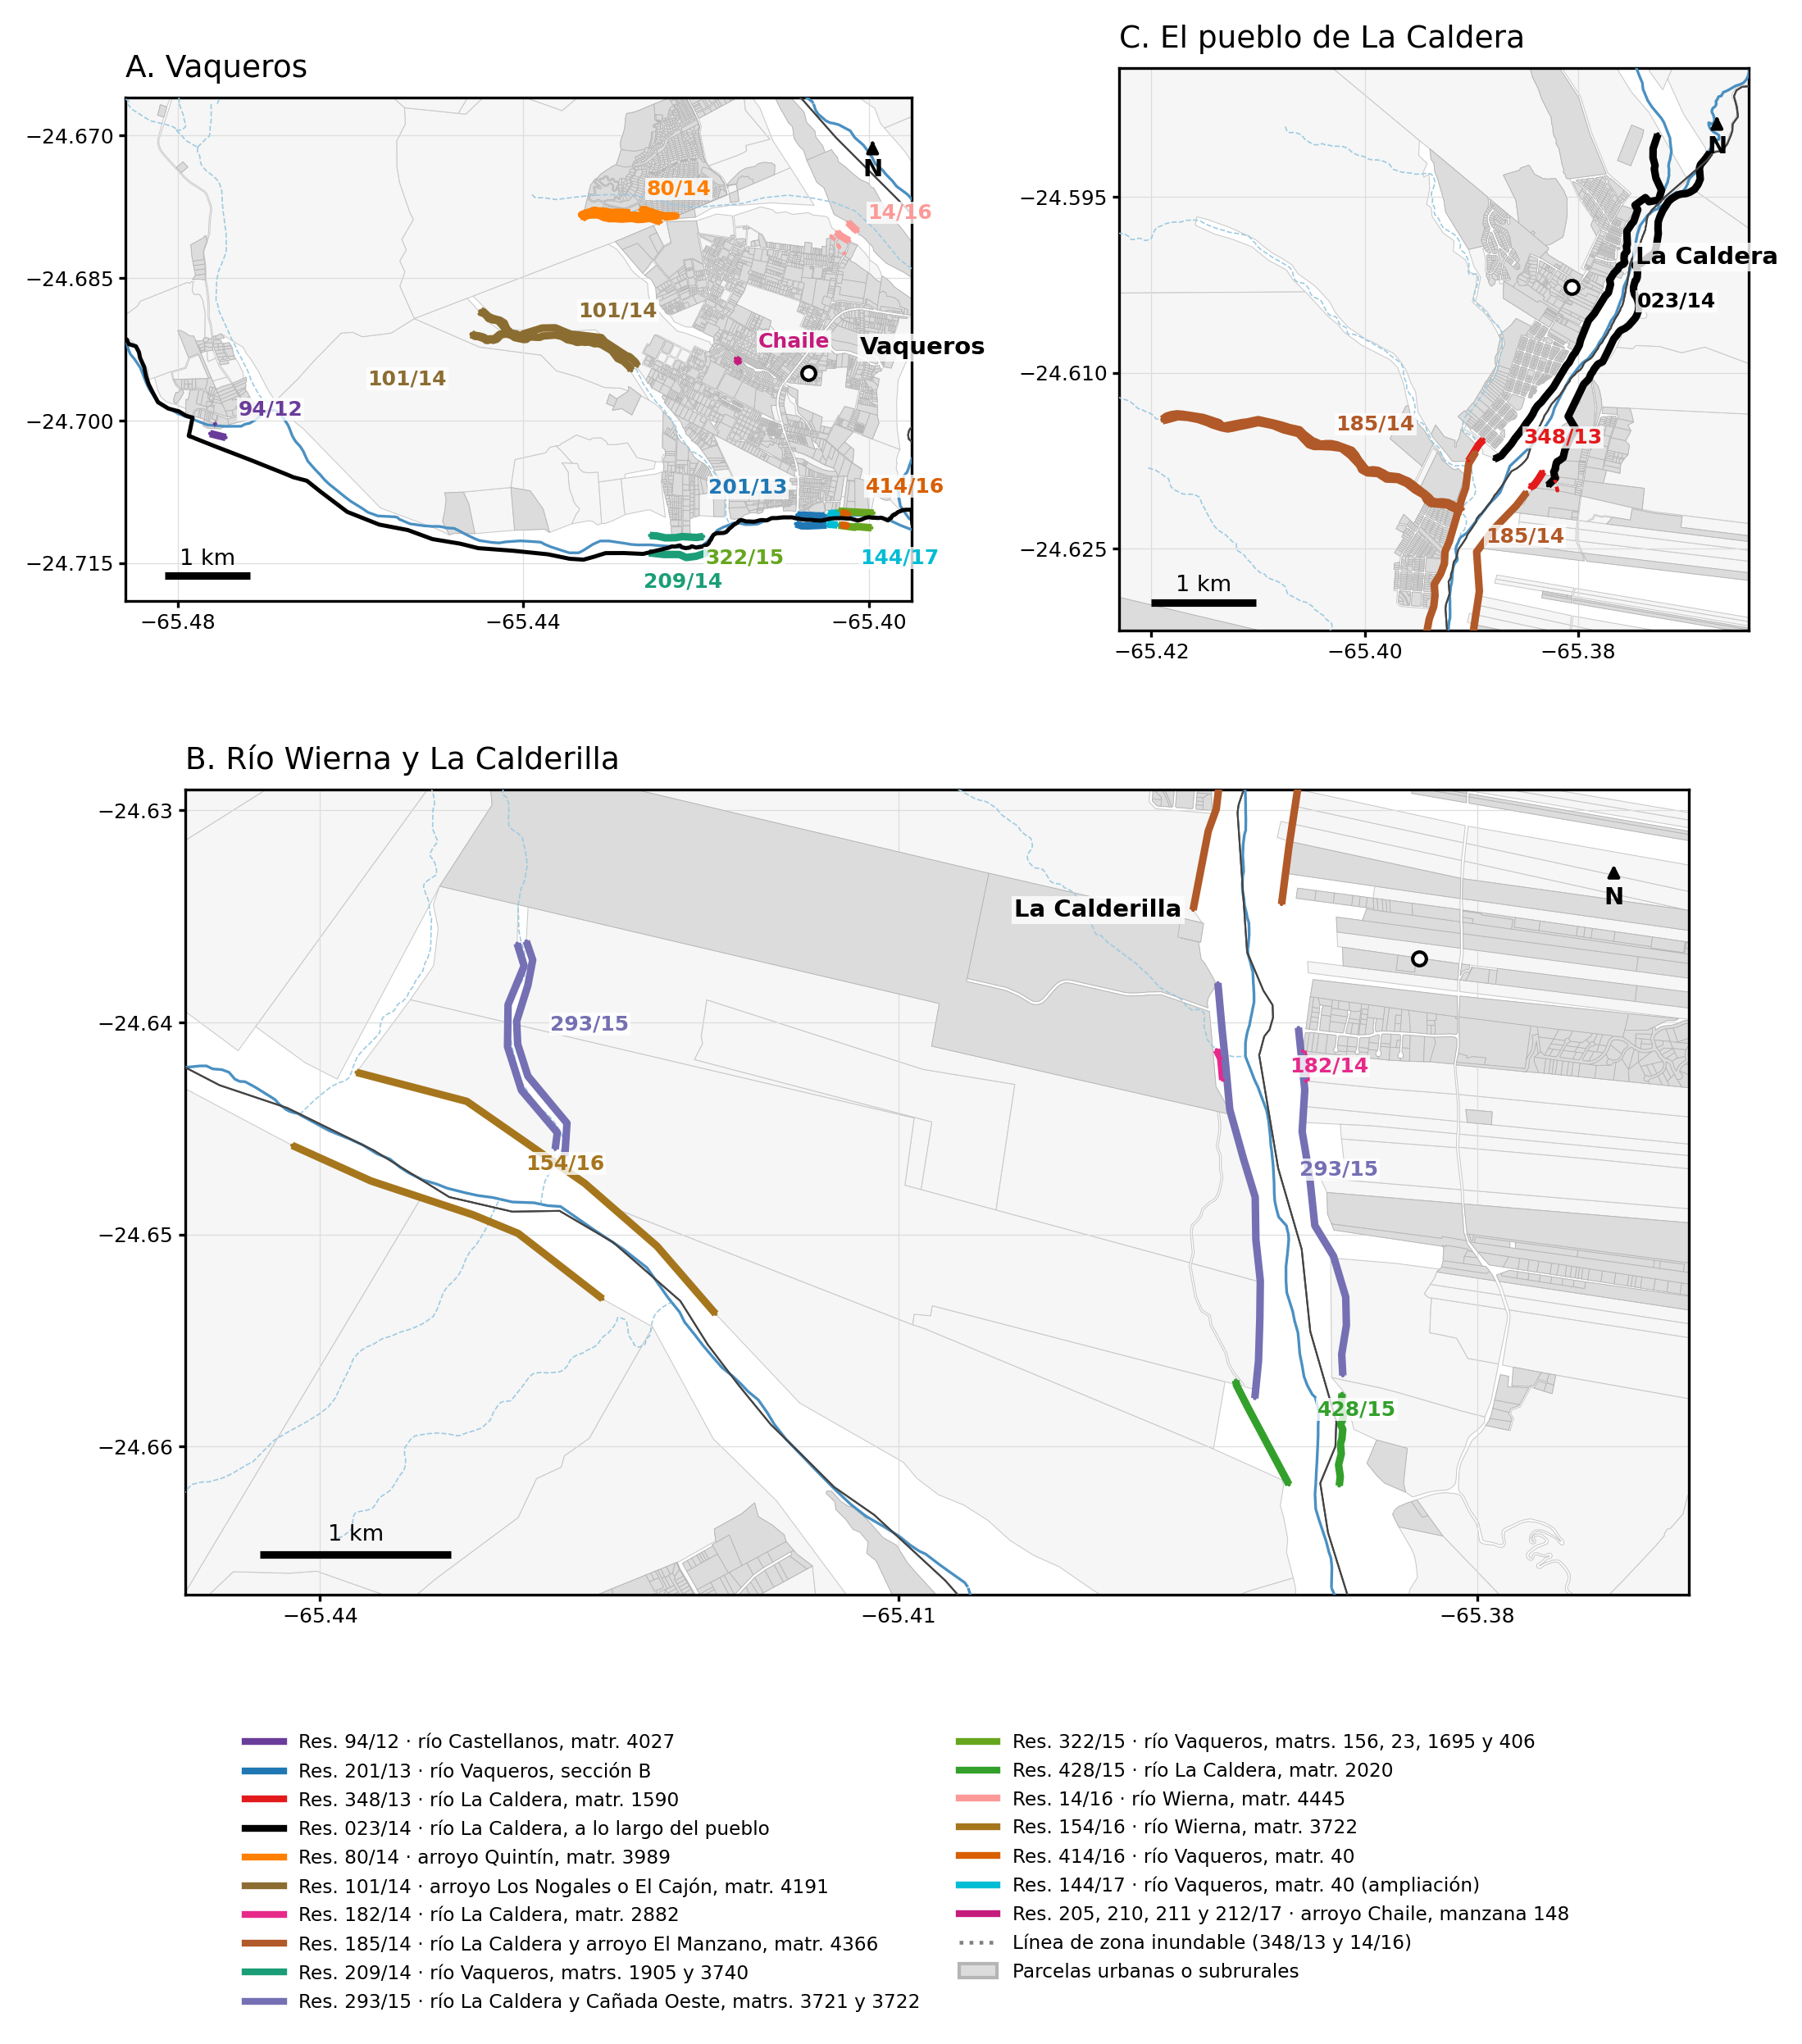
\includegraphics[width=\textwidth,height=0.80\textheight,keepaspectratio]{fig-ribera-edictos.png}
\caption[Las líneas de ribera con coordenadas publicadas]{\textbf{Las líneas de ribera con coordenadas publicadas.} Los puntos de vinculación de veinte resoluciones de la Secretaría de Recursos Hídricos (dictadas entre 2012 y 2017; las cuatro del arroyo Chaile, en un solo color), unidos en el orden de su numeración, sobre la capa catastral. Línea continua: línea de ribera; punteada: línea de zona inundable. A: Vaqueros; B: el río Wierna y La Calderilla; C: el pueblo de La Caldera. No se dibujan las Resoluciones 6/14 y 7/14, cuyos avisos publicaron la tabla de la 023/14. Elaboración propia con las coordenadas de los avisos del Boletín Oficial ---ediciones y órdenes de publicación en la ficha y en la planilla del repositorio cartográfico---, tomadas como Gauss-Krüger faja 3 sobre POSGAR 94 (EPSG:22183) cuando el aviso no declara el marco y leídas según su magnitud cuando los rótulos X e Y están invertidos; la capa «Catastro Urbano y Rural» (IDESA, septiembre de 2026, orientativa) y la hidrografía del IGN. La diferencia entre POSGAR 94 y POSGAR 2007, marco del Mapa Nº~2, es inferior a un metro a esta escala. Elaboración propia; dibujo de \texttt{scripts/mapa\_ribera.py} del repositorio \texttt{mapas\_caldera} (apéndice \ref{cap:fuentes}).}\label{fig:riberaedictos}
\end{figure}

\begin{ficha}{Coordenadas publicadas, edicto por edicto}
\begin{itemize}[leftmargin=*,nosep]
\item \textbf{Res.\ 94/12}, río Castellanos, matrícula 4027: 4 vértices (V9, V10, V13, V14); el edicto rotula «Longitud» y «Latitud» columnas que contienen coordenadas planas.
\item \textbf{Res.\ 201/13}, río Vaqueros, sección B: 13 puntos en la margen izquierda y 5 en la derecha, «Coordenadas Posgar».
\item \textbf{Res.\ 348/13}, río La Caldera, matrícula 1590: 4 y 4 puntos, más 3 de zona inundable.
\item \textbf{Res.\ 80/14}, arroyo Quintín o Pacará, matrícula 3989: 20 y 16 puntos, «Gauss Kruger».
\item \textbf{Res.\ 185/14}, matrícula 4366: 7 y 14 puntos sobre el río La Caldera, 43 y 49 sobre el arroyo El Manzano. \textbf{Son 113, la cifra que da este capítulo.}
\item \textbf{Res.\ 428/15}, río La Caldera, matrícula 2020: 13 y 4 puntos.
\item \textbf{Res.\ 14/16}, río Wierna, matrícula 4445: 3 y 3 puntos, más 4 de línea de inundación; columnas rotuladas «Y, X», con la coordenada este bajo «Y».
\item \textbf{Res.\ 144/17}, río Vaqueros, matrícula 40 (ampliación): 4 y 4 puntos; el edicto llama X a la coordenada norte e Y a la este.
\item \textbf{Res.\ 023/14}, río La Caldera a lo largo del pueblo, sin matrícula: 58 puntos en la margen derecha y 76 en la izquierda, en el anexo vinculado a los avisos de los B.O.\ Nº 19.250 y 19.251 (orden 100039394); columnas «Y, X» con la norte bajo «Y».
\item \textbf{Res.\ 101/14}, arroyo Los Nogales Norte o El Cajón, matrícula 4191 (B.O.\ Nº 19.299, orden 100041196): 23 y 37 puntos en el cauce principal y 17 y 13 en un brazo que el aviso titula «Los Nogales Sur»; un bloque dice «Matrícula N° 491», el punto LRI-8 se repite y el LRI-50 y el LRD-50 tienen las mismas coordenadas. Llama X a la norte.
\item \textbf{Res.\ 182/14}, río La Caldera, matrícula 2882, La Calderilla (B.O.\ Nº 19.347, orden 100042593): 3 y 3 puntos, con rótulos opuestos en cada margen.
\item \textbf{Res.\ 209/14}, río Vaqueros, matrículas 1905 y 3740 (B.O.\ Nº 19.356, orden 400005047): 8 y 6 puntos, «Gauss Kruger».
\item \textbf{Res.\ 293/15}, matrículas 3721 y 3722, Finca Wierna (B.O.\ Nº 19.666, orden 400007168): 10 y 11 puntos sobre el río La Caldera, 8 y 7 sobre la Cañada Oeste. Llama X a la norte.
\item \textbf{Res.\ 322/15}, río Vaqueros, matrículas 156, 23, 1695 y 406 (B.O.\ Nº 19.675, orden 100051198): 2 y 4 puntos; columnas «Y, X» con la este bajo «Y».
\item \textbf{Res.\ 414/16}, río Vaqueros, matrícula 40 (B.O.\ Nº 19.931, orden 100057811): 4 y 3 puntos. Llama X a la norte.
\item \textbf{Res.\ 154/16}, río Wierna, matrícula 3722 (B.O.\ Nº 20.136, orden 400010474): 5 y 5 puntos, redondeados al metro. Llama X a la norte.
\item \textbf{Res.\ 205, 210, 211 y 212/17}, arroyo Chaile, parcelas 32 a 29 de la manzana 148 de Vaqueros (B.O.\ Nº 20.249 y 20.253): dos puntos por margen cada una, cuatro decimales, columnas «Y, X» con la este bajo «Y». Un punto de la 205/17 (X = 726931,0916) no se dibuja.
\end{itemize}
\textit{Quinientos treinta y cinco puntos en total, contando una vez por resolución los puntos de borde que dos resoluciones comparten. Transcripción del texto de cada edición, cotejada contra la imagen de la página donde la capa de texto era dudosa. La planilla, con edición, página, orden de publicación y fecha de consulta por punto, integra el repositorio cartográfico del libro (\texttt{datos/ribera/}).}
\end{ficha}

\begin{cautela}
\textbf{Lo que el dibujo confirma, lo que muestra y lo que no puede mostrar.}

\textbf{Confirma dos cifras del libro.} La Resolución 185/14 publica 113 puntos, y el último punto de la margen derecha de la 201/13 queda a trece metros y medio del último de la ampliación de la 144/17: la continuidad del río Vaqueros que este capítulo afirmaba se ve en el plano.

\textbf{Muestra que el marco de referencia no es uniforme.} De las veinte resoluciones, diez no declaran el sistema y una rotula como geográficas coordenadas planas. Once llaman X a la coordenada norte ---la convención geodésica---, ocho a la este, y la 182/14 usa una convención distinta en cada margen del mismo aviso. La 154/16 publica valores redondeados al metro; las del Chaile, con cuatro decimales. Con las coordenadas publicadas, cualquiera puede reproducir el trazo; con los rótulos tal como están, no sin interpretar.

\textbf{Y no muestra lo que falta.} No están aquí la 383/14 ni la 142/14 y su rectificación 236/14, cuyas coordenadas se remitieron a la sede, ni las determinaciones que, desde la 467/15 de diciembre de 2015, hicieron lo mismo. Tampoco la 6/14 ni la 7/14, porque lo que sus avisos publicaron es la línea del pueblo, que está dibujada una sola vez, como 023/14. Lo que se ve es todo lo que la serie publicó con coordenadas, no todas las líneas que el organismo fijó.
\end{cautela}

\begin{cautela}
Un apunte toponímico, registrado sin conclusión. El arroyo cuya línea de ribera se determinó en abril de 2014 se denomina \textbf{Los Nogales Norte o El Cajón}, y atraviesa la Finca Vaqueros. Los loteos afectados por los aluviones de 2018 y 2019 en el municipio vecino se llaman \textbf{El Nogalar} I, II y IV.

La proximidad de los nombres puede indicar continuidad de un mismo accidente geográfico o simple repetición de un topónimo frecuente en la zona --- los nogales abundan en las yungas del corredor. Establecerlo requiere cartografía, no lectura. Se consigna porque, si se tratara del mismo sistema hídrico, la determinación de abril de 2014 alcanzaría a un curso vinculado a los loteos que se inundaron.
\end{cautela}

\begin{cautela}
Dos advertencias documentales, ninguna resuelta.

\textbf{Sobre el expediente.} El sumario del Boletín Oficial Nº 19.466 consigna, para el aviso de la Resolución 383/14, el expediente \textbf{34-167.127/13}, el mismo de la secuencia 395/13--185/14. \textbf{Un solo expediente administrativo cubre la finca entera y sus cuatro cursos de agua}: de él salieron la 395/13, que designó la comisión técnica; la 185/14, que determinó la línea del río La Caldera y del arroyo El Manzano; y la 383/14, la de El Durazno y Guaranguay. Tres actos, un expediente, una matrícula ---la 4366, pese a que el aviso de la 395/13 dice ``1366'' (B.O.\ Nº 19.232, 24/01/2014): la errata está en el aviso mismo, no en la lectura del escaneo.

\textbf{Sobre las coordenadas.} Los avisos de las Resoluciones 6/14 y 7/14 (B.O.\ Nº 19.232 y 19.233, 24 y 27/01/2014; órdenes 100038934 y 100038932) publican la misma tabla de ciento treinta y cuatro puntos, y \textbf{esa tabla es, punto por punto, la del anexo de la Resolución 023/14}: la línea del río La Caldera a lo largo del pueblo, cincuenta y ocho puntos en la margen derecha y setenta y seis en la izquierda, cotejados uno a uno contra el facsímil del anexo. Tres cosas se siguen.

\textbf{La tabla no se arrastró de la 023/14.} Los dos avisos salieron entre dos y tres semanas antes de que la 023/14 se dictara (06/02/2014) y casi un mes antes de que se publicara (19/02/2014). La tabla existía antes: es, con toda probabilidad, la determinación que la Dirección General de Planificación Hídrica hizo «por Administración» y que la 023/14 cita a fojas 3 de su expediente.

\textbf{Al menos la 7/14 publicó coordenadas ajenas.} Los ciento treinta y cuatro puntos van, de norte a sur, de 7.281.221 a 7.277.907 metros: el tramo del pueblo. La 7/14 recae sobre la matrícula 3584 de La Calderilla, y la determinación publicada más próxima en esa localidad ---la 182/14, matrícula 2882--- está unos dos kilómetros y medio más al sur que el último punto de la tabla. Dónde está la matrícula 3593 de la 6/14 este libro no lo sabe; si no está en el tramo del pueblo, sus coordenadas tampoco son las suyas. La capa catastral lo resolvería si la matrícula sigue vigente.

\textbf{Y la línea del pueblo quedó publicada tres veces bajo tres actos distintos}: dos que se refieren a inmuebles particulares y fueron determinados por comisiones técnicas ---la de la 6/14 la designó la Resolución 322/12---, y uno pedido por el intendente y hecho por la propia Administración. Qué línea rige para las matrículas 3593 y 3584 es una pregunta que sólo el organismo puede contestar; el apéndice \ref{cap:pedidos} la formula.
\end{cautela}

\begin{cautela}
Un quinto acto del mismo período cierra el círculo de otra manera.

Los Boletines Nº 19.250 y 19.251, del 19 y el 21 de febrero de 2014, publican la \textbf{Resolución Nº 000023/14} de la Secretaría de Recursos Hídricos con un título ---«Río La Caldera, Pueblo La Caldera»--- y la leyenda «ver anexo». El anexo, vinculado a los dos avisos en la edición web, contiene la resolución completa.

\end{cautela}

\begin{ficha}{Resolución SRH Nº 000023 del 6 de febrero de 2014 --- expte.\ 0090034-96837/2013}
\textbf{Origen:} nota del intendente de La Caldera, \textbf{Luis G.\ Mendaña\index{Mendaña, Luis Gerardo}}, que pide la línea de ribera de ambas márgenes del río La Caldera a lo largo del pueblo, con una imagen satelital (fs.\ 1 y 2). La Dirección General de Planificación Hídrica informa que la determinación \textbf{«se ha realizado por Administración»}, con coordenadas y plano, y que \textbf{«estará sujeta a la construcción de defensas con gaviones a lo largo de la misma»}, tramitada por expediente 34-253.934/13 (fs.\ 3). Dictamen jurídico por el art.\ 126 del Código de Aguas y el Decreto 1989/02 (fs.\ 7).

\textbf{Art.\ 1:} aprueba la designación del \textbf{Geól.\ Jorge G.\ Torres\index{Torres, Jorge G.}} para las tareas de determinación.

\textbf{Art.\ 2:} \textbf{determina la línea de ribera sobre ambas márgenes del río La Caldera a lo largo del pueblo}, con sus coordenadas: \textbf{134 puntos}, 58 en la margen derecha y 76 en la izquierda.

\textbf{Art.\ 3:} \textbf{advierte a la Municipalidad que la determinación estará sujeta a la construcción de defensas con gaviones} a lo largo de ella.

Arts.\ 4 y 5: publicación por dos días y notificación a Inmuebles. Firma el secretario Alfredo Fuertes.
\end{ficha}

\begin{cautela}

\textbf{La primera:} Jorge G.\ Torres\index{Torres, Jorge G.} es el autor de la presentación institucional sobre línea de ribera que este capítulo utiliza como fuente del procedimiento, y figura en diciembre de 2025 como Director General de Cuencas y Política Hídrica de la provincia. En febrero de 2014 fue designado para determinar la línea de ribera del río La Caldera \textbf{a la altura del pueblo}. La continuidad entre quien ejecutó la tarea en el terreno y quien hoy conduce el área es completa.

La lámina \ref{fig:otbn} traza esa línea sobre el pueblo.

\textbf{La segunda, y es una corrección.} Este libro había registrado esta resolución como publicada sin contenido y la contaba entre los anexos no publicados. No lo es: el anexo está vinculado a los dos avisos y trae las coordenadas completas. \textbf{El acto más pertinente al ejido urbano de La Caldera es, al contrario, uno de los que publicaron sus coordenadas}, aunque en un formato ---una copia escaneada vinculada a un aviso de dos líneas--- que ninguna búsqueda de texto encuentra.

\textbf{La tercera: la línea de ribera del pueblo quedó condicionada a una obra.} El artículo 3 sujeta la determinación a defensas con gaviones que en febrero de 2014 se tramitaban por un expediente propio. La línea se trazó contando con defensas que todavía no existían, y es ese expediente ---no la resolución--- el que dice si se construyeron (capítulo \ref{cap:defensas}). Y el pedido lo hizo el intendente: el municipio promovió la determinación sobre su propio pueblo.
\end{cautela}

Y la matrícula 4366 gana un nombre y una dimensión. Se llama \textbf{Finca La Caldera o Getsemaní}, y está atravesada por al menos \textbf{cuatro cursos de agua}: el río La Caldera, el arroyo El Manzano, el arroyo El Durazno y el arroyo Guaranguay. Las dos determinaciones de 2014 --- julio y diciembre --- cubren dos cursos cada una.

Eso reordena la pregunta dominial que este libro arrastra. La Resolución 646D/21 aprobó el plano del loteo El Durazno sobre la \textbf{matrícula 6.558}. Las líneas de ribera de sus arroyos se determinaron sobre la \textbf{matrícula 4366}. Si la 6.558 proviene de la 4366 por desmembramiento --- lo que la numeración sugiere y nada prueba ---, entonces el loteo se asienta sobre una finca cuyos cuatro cursos de agua fueron relevados por el Estado entre 2013 y 2014, y la línea de ribera de dos de ellos recae directamente sobre su suelo.

Es la comprobación más importante que le queda a este capítulo, y se hace con un informe de dominio de la Dirección General de Inmuebles.

\begin{cautela}
\textbf{Después de la serie, el mismo patrón.} La serie de 2013 a 2015 no fue la última palabra. El Boletín Oficial Nº 19.951, del 27 de enero de 2017, publica el edicto de la \textbf{Resolución Nº 360 del 7 de noviembre de 2016} de la Secretaría de Recursos Hídricos, expediente 34-171.172/15.

\end{cautela}

\begin{ficha}{Resolución SRH Nº 360/16 --- B.O.\ Nº 19.951, pág.\ 71}
Aprueba la determinación de la línea de ribera realizada por la Comisión Técnica en \textbf{ambas márgenes del río Wierna}, en la zona de los inmuebles de \textbf{matrículas 4097, 4953, 391, 389, 1268, 3718 y 3438} del departamento La Caldera. Integran la comisión el geólogo \textbf{Jorge Genaro Torres} y el ingeniero civil Carlos Enrique Cerezo.

``Las coordenadas Posgar de las líneas de ribera determinadas en ambas márgenes de los cauces mencionados \textbf{se encuentran a disposición de los interesados en la sede} de la Secretaría de Recursos Hídricos.''

Apelable ante el Tribunal de Aguas en diez días hábiles. Firman el secretario Alfredo Fuertes y la asesora legal Sandra Mabel Siegrist; edicto fechado el 16 de noviembre de 2016 y publicado el 26 y el 27 de enero de 2017.
\end{ficha}

\begin{cautela}

Tres observaciones. La fórmula es literalmente la de las Resoluciones 142/14 y 383/14, con otro firmante, dos años después: la omisión de las coordenadas no fue un rasgo de un asesor ni de una racha. El geólogo que la Resolución 023/14 designó para el río La Caldera sigue integrando comisiones del departamento en 2016. Y el río Wierna ---donde el capítulo \ref{cap:amparo} registra cuatro canteras y el capítulo \ref{cap:defensas} un encauzamiento provincial en 1980--- tiene línea de ribera determinada desde 2016 sobre siete inmuebles cuya relación con esas canteras y obras este libro no estableció.
\end{cautela}

\section{2017: la línea de ribera que pide el propio Estado}

Este capítulo miró hasta acá quién pide una determinación de línea de ribera: un
peticionante particular, un loteo, un vecino. Falta un tercer solicitante, y es el más
revelador.

\begin{ficha}{Secretaría de Comunicación de la Provincia de Salta, 16 de agosto de 2017}
El secretario de Recursos Hídricos, \textbf{Alfredo Fuertes}, se reúne con profesionales de la
empresa \textbf{Supercemento}, la consultora \textbf{IHTSA} y la empresa \textbf{Aguas del
Norte} para coordinar las tareas de la obra del \textbf{Acueducto Norte}.

Los participantes destacan como punto principal \textbf{la determinación de la línea de ribera
del río La Caldera en la zona de emplazamiento de la planta de tratamiento}, porque de ese
trabajo depende que puedan diseñarse las defensas apropiadas. Se explican además los
requisitos necesarios para los cruces de los cauces de \textbf{Los Naranjos, Guaranguay y
Wierna}.

El acueducto tendrá una capacidad de \textbf{1.100 metros cúbicos por hora} y abastecerá a
toda la zona norte de la ciudad de Salta y a los pobladores de Vaqueros.

Participa, por la Provincia, el \textbf{director de Planificación Hídrica, Jorge Torres}.
\end{ficha}

\textbf{Primera: aparece Guaranguay otra vez.} Es el mismo arroyo cuya línea de ribera se
determinó en diciembre de 2014 sin publicar coordenadas. Dos años y ocho meses después, el
propio Estado necesita saber dónde está esa línea para cruzarlo con un acueducto. El dato que
no se publicó para el vecino hacía falta para la obra.

\textbf{Segunda: el instrumento sirve, y el Estado lo sabe.} Cuando la obra es del Estado, la
determinación de línea de ribera no es un trámite ni un requisito formal: es el paso previo
sin el cual no pueden diseñarse las defensas. Lo dice la propia comunicación oficial. Es la
mejor prueba disponible de que el instrumento no es decorativo, y de que su ausencia en El
Durazno no se explica por irrelevancia técnica.

\textbf{Y tercera: Jorge Torres cambia de lugar en la estructura.} En febrero de 2014 la
Resolución 023/14 lo designa \textbf{como geólogo} para determinar la línea de ribera del río
La Caldera a la altura del pueblo. En agosto de 2017 participa \textbf{como director de
Planificación Hídrica}. Se consigna el recorrido porque explica por qué su nombre aparece en
los dos extremos de este capítulo, y no como imputación de ninguna clase.

\begin{cautela}
La fuente es \textbf{un parte de prensa oficial}, no un expediente. Acredita que la reunión
existió y qué se dijo en ella; \textbf{no acredita que la determinación se haya hecho}. Este libro no encontró la resolución de determinación, y la duda queda abierta: si el Estado determinó esa línea, el acto debería existir; si no la determinó, la obra se diseñó sin ella. Lo que sí encontró es una comisión técnica de 2015 sobre el río La Caldera en el catastro 4049, con Torres entre sus integrantes, cuyo aviso el índice del Boletín atribuye a Aguas del Norte (véase más adelante en este capítulo).
\end{cautela}

\section{Trece meses antes, el mismo organismo hizo lo contrario}

Existe un edicto anterior del mismo organismo, sobre el mismo río, en el mismo departamento y con la misma firma. Sirve de control y convierte una impresión en una comparación.

\begin{ficha}{Resolución Nº 348 del 19/11/2013 --- B.O.\ Nº 19.213, 23 y 26 de diciembre de 2013}
Determinación de la línea de ribera en ambas márgenes del \textbf{río La Caldera}, en la zona del inmueble de \textbf{matrícula catastral Nº 1590, localidad de La Calderilla}, departamento La Caldera.

\textbf{El edicto publica las coordenadas.} Cuatro puntos Posgar de margen izquierda (LRi01 a LRi04) y cuatro de margen derecha (LRd05 a LRd08), con sus valores X e Y completos. \textit{(Más adelante este capítulo cuenta once pares publicados en este edicto; la diferencia con los ocho de la línea de ribera debe cotejarse contra el original.)}

\textbf{El edicto determina además la zona inundable}, con su propia tabla de coordenadas, y advierte que ``puede sufrir inundaciones durante las crecidas extraordinarias''.

\textbf{Y transcribe el artículo 172 del Código de Aguas}, con sus restricciones al uso del suelo.

Firma: Dr.\ Matías J.\ Brogin\index{Brogin, Matías J.}, Asesor Legal. Orden de publicación 400004557.
\end{ficha}

\begin{cautela}
Póngase al lado el edicto de la Resolución 383/14, publicado trece meses después, en enero de 2015, por la misma Secretaría y con la firma del mismo asesor legal, sobre los arroyos El Durazno y Guaranguay.

\begin{center}\small
\begin{tabular}{@{}p{4.4cm}p{3.8cm}p{3.8cm}@{}}
\toprule
& \textbf{Res.\ 348/13} (dic.\ 2013) & \textbf{Res.\ 383/14} (ene.\ 2015) \\
\midrule
Coordenadas Posgar & \textbf{Publicadas en el edicto} & Remitidas a la sede \\
Zona inundable & \textbf{Determinada y publicada} & No mencionada \\
Art.\ 172 del Código de Aguas & \textbf{Transcripto} & No mencionado \\
\bottomrule
\end{tabular}
\end{center}

Este libro había observado que el edicto de 2015 remitía las coordenadas a Avenida Bolivia 4650 y que eso volvía difícil el ejercicio del derecho a apelar. La observación se sostenía sobre el sentido común. Ahora se sostiene sobre un precedente: \textbf{el organismo sí publicaba coordenadas, y lo había hecho poco antes, en el mismo departamento}. No era una imposibilidad técnica ni una práctica uniforme.

\textbf{Corresponde una advertencia de peso.} El edicto es una síntesis de la resolución, no la resolución. Que el edicto de 2015 no mencione la zona inundable ni el artículo 172 \textbf{no prueba} que la Resolución 383/14 no los haya determinado o invocado. Puede haberlo hecho y el edicto haber salido más escueto. Establecerlo requiere el texto de la resolución, no su publicación.

Lo que queda probado es más acotado y sigue siendo sustancial: \textbf{lo que llegó a conocimiento público fue distinto en un caso y en otro}, y el caso que llegó mermado es el que recae sobre los arroyos que se desbordaron cuatro años después.
\end{cautela}

\subsection*{Y en 2016, con la misma firma, volvió a publicarlo todo}

\begin{ficha}{Resolución Nº 14 del 15/01/2016 --- B.O.\ Nº 19.740 y 19.741, 15 y 16 de marzo de 2016}
Expediente 34-125.733/15. Aprueba la determinación de la línea de ribera realizada por la Comisión Técnica en \textbf{ambas márgenes del río Wierna}, en la zona de la matrícula 4445, Fracción 195, Finca «Vaqueros», localidad Vaqueros.

\textbf{Publica las coordenadas}: tres puntos Gauss-Krüger por margen (LRI-01 a 03 y LRD-01 a 03).

\textbf{Determina una línea de inundación} sobre la margen derecha, con cuatro puntos (Li-01 a Li-04), declara que esas zonas «pueden sufrir inundaciones durante las crecidas extraordinarias» y \textbf{transcribe el artículo 172 del Código de Aguas}.

Edicto del 25 de enero de 2016. Firman el secretario Alfredo Fuertes y el asesor legal \textbf{Matías J.\ Brogin}\index{Brogin, Matías J.}.

La comisión se había aprobado por la Resolución 273/15 del 13 de agosto de 2015 (B.O.\ Nº 19.614 y 19.615) para «ambas márgenes del \textbf{río Trancas}», con el ingeniero Antonio Alejandro Forns\index{Forns, Antonio Alejandro}, el geólogo Teodoro Chafatinos y el ingeniero Lucas Vidal.
\end{ficha}

\begin{cautela}
Este edicto cambia el peso de la comparación anterior. La Resolución 348/13 no fue un caso único: un año después de publicar sin coordenadas ni zona inundable la línea de El Durazno, el mismo organismo, con el mismo asesor legal, publicó para un inmueble de Vaqueros las coordenadas, la línea de inundación y el artículo 172. La forma completa del edicto existía antes y después de la Resolución 383/14. Lo que la diferencia no es el período ni el firmante.

Y deja una discordancia que este libro registra sin resolver: la comisión se designó para el río Trancas y la determinación se aprobó sobre el río Wierna, en el mismo expediente y el mismo inmueble. Puede tratarse de dos nombres del mismo tramo o de un error de uno de los dos edictos. \pendiente{aclaración de la Secretaría sobre el curso del expediente 34-125.733/15}
\end{cautela}

\begin{ficha}{Resolución Nº 144/17 --- B.O.\ Nº 20.042 y 20.043, 15 y 16 de junio de 2017}
Expediente 34-202.169/15. Modifica parcialmente el artículo 1º de la \textbf{Resolución 414 del 5 de noviembre de 2016} ---fecha que la numeración de la serie contradice; véase la tabla--- y aprueba la \textbf{ampliación} de la determinación de la línea de ribera en ambas márgenes del \textbf{río Vaqueros}, en la zona que colinda con la \textbf{matrícula 40}. Publica cuatro puntos por margen (LRmd1a a 4a, LRmi5a a 8a). Edicto del 11 de mayo de 2017; firman Fuertes y la asesora legal Sandra Mabel Siegrist.
\end{ficha}

El expediente del río Vaqueros quedó completo con la comisión de la Resolución 147/16 y la determinación de la 414/16. Entre la margen derecha y la izquierda median unos ciento treinta a ciento cuarenta metros; con la ampliación de 2017, la margen derecha suma unos doscientos cuarenta metros de poligonal publicada. Y la comisión tiene una composición que ninguna otra de las leídas repite: tres miembros, uno de ellos \textbf{ingeniero hidráulico}, que es la especialidad que el artículo 3º del Anexo I pone en primer lugar.

Dos datos más para la serie. La omisión de las coordenadas tampoco fue un rasgo de la asesora que firma la serie desde 2016 ---y edictos del organismo al menos desde agosto de 2014, capítulo \ref{cap:redes}---: en noviembre de 2016 su edicto sobre el Wierna (Resolución 360/16) las remitió a la sede, y un mes después, en diciembre, su edicto sobre el río Vaqueros (Resolución 414/16) las publicó, como volvió a hacerlo seis meses más tarde con la ampliación (Resolución 144/17). Y una determinación publicada puede ampliarse después: la de la matrícula 40 se modificó a los seis meses. Qué motivó la ampliación, y si el tramo agregado coincide con una subdivisión o un proyecto sobre ese inmueble, es lo que diría el expediente. \pendiente{fundamentos de la ampliación de la Resolución 414/16 por la 144/17}

\subsection*{2016 y 2017: el relevamiento siguió}

La serie de 2013 a 2015 no se cerró en diciembre de 2015. Los avisos de 2016 muestran que el departamento siguió bajo relevamiento, con los mismos técnicos y dos cursos nuevos.

{\small
\setlength{\LTpre}{0.6em}\setlength{\LTpost}{1.2em}
\begin{longtable}{@{}p{2.3cm}p{2.6cm}p{7cm}@{}}
\toprule
\textbf{Acto} & \textbf{Expediente} & \textbf{Objeto} \\
\midrule
\endhead
Res.\ 154/16 (17/05/16) & 34-259.760/14 & \textbf{Determinación}: \textbf{río Wierna}, matrícula 3722, Finca Wierna ---el expediente de la comisión 74/15 y de la determinación 293/15 sobre el río La Caldera---. Con coordenadas, cinco puntos por margen \textbf{redondeadas al metro}. Edicto del 23/05/2016, \textbf{publicado el 2 y 3/11/2017}, diecisiete meses después \\
Res.\ 14/16 (15/01/16) & 34-125.733/15 & \textbf{Determinación}: río Wierna (comisión por el Trancas), matrícula 4445, Finca Vaqueros. \textit{Con coordenadas y línea de inundación} \\
Res.\ 122/16 (21/04/16) & 34-62.718/16 & \textbf{Comisión}: arroyo Quintín, matrícula 4953, Finca Vaqueros. Torres y Cerezo. B.O.\ 6 y 7/06/2016 \\
Res.\ 282/16 (26/08/16) & 34-202.924/15 & \textbf{Determinación}: río La Caldera, matrícula 1499, Finca San Jorge, La Calderilla. \textit{Coordenadas remitidas a la sede}; cita el «Dcto.\ 1898/02». B.O.\ 28 y 29/09/2016 \\
Res.\ 290/16 (07/09/16) & 34-178.741/16 & \textbf{Comisión}: \textbf{arroyo Chaile}, matrícula 1534. El ingeniero Marcelo Toigo y el geólogo Enrique Chalabe. B.O.\ 20 y 21/10/2016 \\
Res.\ 291/16 (07/09/16) & 34-116.088/16 & \textbf{Comisión}: río La Caldera, \textbf{matrícula 4146}, Fracción 71, La Calderilla. Torres y el ingeniero Emanuel Caro. B.O.\ 30/09 y 03/10/2016 \\
Res.\ 147/16 (11/05/16) & 34-202.169/15 & \textbf{Comisión}: río Vaqueros, catastro 40. Integran el ing.\ en construcciones Rolando Chávez, el \textbf{ingeniero hidráulico} Víctor Zacarías Pérez y el geólogo Héctor Saravia Navamuel. B.O.\ 28 y 29/06/2016 \\
Res.\ 414/16 (05/11/16) & 34-202.169/15 & \textbf{Determinación}: río Vaqueros, matrícula 40. \textit{Con coordenadas publicadas} (tres puntos en la margen derecha, cuatro en la izquierda). Fecha según la Res.\ 144/17: el edicto no la consigna. \textbf{La fecha no cuadra con la numeración}: la 360/16 es del 7 de noviembre y la 389/16 del 21, de modo que la 414 difícilmente sea del 5 de noviembre, que además fue sábado; el 5 de diciembre, lunes, encaja con la serie, pero este libro no lo establece. B.O.\ 29/12/2016 y 02/01/2017; ampliada por la 144/17 \\
Res.\ 389/16 (21/11/16) & 34-248.094/16 & \textbf{Determinación «realizada por Administración»}: arroyo Quintín, matrícula 4953, Finca Vaqueros. \textit{Coordenadas remitidas a la sede}; cita el «Dcto.\ 1898/02». Firma el geólogo Torres como director general de Planificación Hídrica. B.O.\ 19 y 20/12/2016 \\
Res.\ 360/16 (07/11/16) & 34-171.172/15 & \textbf{Determinación}: río Wierna, siete matrículas. \textit{Coordenadas remitidas a la sede} \\
Res.\ 424, 425, 426 y 427/16 (14/12/16) & 34-257.289/16, 34-229.971/16, 34-257.277/16 y 34-229.967/16 & \textbf{Cuatro comisiones}: arroyo Chaile o Teodolinda, matrículas 2343, 2345, 2342 y 2344 (Vaqueros, sección A, manzana 148, parcelas 30, 32, 29 y 31). Torres y Caro. B.O.\ Nº 19.934 y 19.935, 4 y 5/01/2017; dos de los títulos del índice dicen «río La Caldera», y el aviso de la 427/16 lo dice también en su cuerpo \\
Res.\ 205, 210, 211 y 212/17 & 34-229.971/16, 34-257.289/16, 34-229.967/16 y 34-257.277/16 & \textbf{Cuatro determinaciones}: arroyo Chaile o Teodolinda, matrículas 2345, 2343, 2344 y 2342. \textit{Con coordenadas publicadas}, dos puntos por margen cada una. Edictos de abril de 2018, publicados el 25 y 26/04 y el 3 y 4/05/2018 \\
Res.\ 279/17 (09/08/17) & 34-116.088/16 & \textbf{Determinación}: río La Caldera, matrícula 4146, Fracción 71, La Calderilla; cierra la comisión de la 291/16. \textit{Coordenadas remitidas a la sede}; cita el «Dcto.\ 1.898/02». Edicto del 18/08/2017, B.O.\ 20 y 21/09/2017 \\
\bottomrule
\end{longtable}
}

La Resolución 154/16 agrega un caso de demora extrema: firmada por Brogin en mayo de 2016, se publicó en noviembre de 2017, cuando los edictos del organismo ya los firmaba otra asesora. Y sus coordenadas, a diferencia de todas las demás publicadas, no tienen decimales: puntos separados por cuatrocientos cincuenta a setecientos cincuenta metros, redondeados al metro, a lo largo de más de dos kilómetros de río.

Todas las comisiones de 2016 invocan el método «geológico-geomorfológico»; las de 2015, «geológico-morfológico». Firman Brogin hasta mediados de año y Siegrist desde septiembre.

\begin{cautela}
Las actuaciones sobre el arroyo Chaile o Teodolinda en Vaqueros muestran algo que ningún otro grupo de la serie mostraba: \textbf{una sola línea de ribera partida en lotes}. Son cuatro parcelas contiguas de una manzana urbana, la 148 de la sección A, con matrículas correlativas (2342 a 2345) y parcelas correlativas (29 a 32). Cada una tiene su expediente, su comisión ---las cuatro del mismo día, con los mismos dos técnicos---, su determinación y sus dos edictos. Pero los puntos forman una sola poligonal: los de borde se repiten de una resolución a la siguiente con las mismas coordenadas. Cada tramo mide entre catorce metros y medio y dieciséis metros y medio por margen ---salvo la margen derecha de la parcela 32, que no se puede medir por el dígito faltante que se señala abajo---; los cuatro juntos, unos sesenta y dos.

La publicación tiene tres defectos menores que, juntos, muestran cómo se armaba. Los nombres de los puntos no son únicos: la parcela 31 y la 32 usan los mismos rótulos (LRmi01, LRmi02, LRmd09, LRmd10) para coordenadas distintas. Un punto compartido figura con un centímetro de diferencia entre dos edictos. Y una coordenada de la parcela 32 se publicó con un dígito de menos (X = 726931,0916, que no corresponde a ningún lugar de la provincia). A eso se suman dos títulos del índice que atribuyen el arroyo al río La Caldera.

Es, por lo tanto, un relevamiento continuo tramitado como cuatro. Qué lo explica ---cuatro propietarios distintos, un fraccionamiento que cada comprador debió completar por su cuenta, o la exigencia de una línea por lote para aprobar construcciones--- es lo que dirían los expedientes. Lo que el Boletín muestra es el resultado: ocho publicaciones pagadas para fijar poco más de sesenta metros de ribera. Las determinaciones llevan número de 2017 y se publicaron en abril y mayo de 2018. La comisión de la parcela 31 sí se publicó: es la Resolución 427/16, del mismo día que las otras tres y con su mismo expediente (B.O.\ Nº 19.934 y 19.935, 4 y 5/01/2017), pero su aviso la dicta para el «río La Caldera» y no para el arroyo Chaile. Una versión anterior de este párrafo la daba por no publicada. \pendiente{solicitantes de los cuatro expedientes}
\end{cautela}

\begin{cautela}
Tres cosas se siguen de esta tabla. La primera cierra una pregunta abierta: la serie del río La Caldera sobre la matrícula 4146 ---determinada por la Resolución 279/17, retomada por la 306/19 y rectificada por la 108/2025--- empieza con la Resolución 291/16, que designó la comisión en septiembre de 2016, en La Calderilla y con el geólogo Torres, y la determinación del 9 de agosto de 2017 la cierra en el mismo expediente, con las coordenadas remitidas a la sede, igual que la rectificación de 2025.  El edicto de la Resolución 306/19 no se leyó: la búsqueda por el número del expediente de 2016 devuelve sólo la comisión y la determinación de 2017, de modo que la 306/19 tramitó, probablemente, con un expediente de numeración nueva. La 279/17, en cambio, es anterior a la reunión de 2017 sobre el Acueducto Norte, y es la candidata más firme para la línea que esa reunión presentaba como pendiente.

La segunda es de nombres: el ingeniero Toigo, que en 2011 integró la comisión de Chacras del Gallinato, integra en 2016 la del arroyo Chaile. Y la matrícula 4953 aparece dos veces en el mismo año, en la comisión del Wierna y en la del Quintín: un mismo inmueble atravesado por dos cursos, con dos expedientes.

La determinación del Quintín de noviembre de 2016 agrega dos rasgos que la serie no tenía. No la hizo una comisión técnica sino, dice el edicto, «la Administración». Y la firma, junto a la asesora legal, el geólogo Jorge Genaro Torres como director general de Planificación Hídrica: el mismo técnico que integró la comisión designada en abril de ese año sobre el mismo arroyo y la misma matrícula, y que integra la mayoría de las comisiones del departamento entre 2015 y 2017, aparece aquí del lado de la autoridad que aprueba y publica. El expediente es otro (34-248.094/16, no el 34-62.718/16 de la comisión), de modo que no puede afirmarse que esta determinación cierre aquella comisión; puede ser un trámite de oficio distinto sobre el mismo tramo.

Hay además una anomalía de expediente. El edicto de la Resolución 131/16, que designa una comisión para el río San Lucas en la matrícula 559 del \textbf{departamento San Carlos}, lleva como referencia el expediente 34-62.718/16: el mismo de la comisión del arroyo Quintín, con la misma comisión (Torres y Cerezo), la misma fecha de edicto (29 de abril de 2016) y la misma firma. Uno de los dos encabezados está mal; es el mismo tipo de arrastre de texto entre edictos que la cita del decreto.

La tercera es de forma. En septiembre de 2016 la misma asesora firmó una determinación con las coordenadas remitidas a la sede y con el decreto mal citado; ocho meses después, otra con las coordenadas publicadas. El formato del edicto no dependía de quién lo firmaba.

La lista no es completa: el buscador ofrece más de quinientos avisos de toda la provincia para estos años, y sólo se revisó una parte de sus páginas. \pendiente{relación entre la comisión de la Resolución 122/16 y la determinación «por Administración» de la 389/16, ambas sobre el Quintín en la matrícula 4953; determinación resultante de la Resolución 290/16 (Chaile, matrícula 1534); coordenadas de la Resolución 279/17; expediente correcto de la Resolución 131/16; comisión de la Resolución 282/16; y revisión de las páginas restantes del listado de 2015--2017}
\end{cautela}

\subsection*{El arroyo Chaile, parcela por parcela (2016--2024)}

Las cuatro parcelas de la manzana 148 no fueron un caso aislado. Una búsqueda por el nombre del arroyo devuelve una serie que llega a 2024.

{\small
\setlength{\LTpre}{0.6em}\setlength{\LTpost}{1.2em}
\begin{longtable}{@{}p{2.4cm}p{3.3cm}p{6.2cm}@{}}
\toprule
\textbf{Acto} & \textbf{Expediente} & \textbf{Objeto y publicación} \\
\midrule
\endhead
Res.\ 251/16 (11/08/16) & 34-103.747/16 & \textbf{Comisión}: «arroyo Seco», matrícula 2821 (sección A, manzana 75, parcela 8D) y parte de la 4953. Torres y Caro. Edicto de junio de 2018: \textbf{publicada casi dos años después} \\
Res.\ 290/16 (07/09/16) & 34-178.741/16 & \textbf{Comisión}: matrícula 1534. La búsqueda por el expediente no devuelve determinación alguna \\
Res.\ 424 a 426/16 y 205 a 212/17 & cuatro expedientes & Manzana 148, matrículas 2342 a 2345. Con coordenadas \\
Sin número (jul.\ 2019) & 0090034-142.128/19 & \textbf{Comisión}: matrícula 5928. Torres y el ing.\ Julio César Zamora \\
Res.\ 327/19 (31/10/19) & 0090034-142.128/19 & \textbf{Determinación}: matrícula 5928. B.O.\ 3 y 4/12/2019 \\
Res.\ 75/2020 (03/03/20) & 0090034-103.747/2016 & \textbf{Determinación de línea de ribera y zona inundable}: «arroyos Vaqueros y Chaile», matrícula 2821 y parte de la 4953. B.O.\ 7 y 8/07/2020 \\
Res.\ 182/2021 (07/09/21) & 0090034-111.930/2021 & \textbf{Determinación}: catastro 1750. B.O.\ 22 y 23/09/2021 \\
Res.\ 51/2022 (27/04/22) & 0090034-170.889/2021 & \textbf{Determinación}: catastro 2318. B.O.\ 6 y 7/06/2022 \\
Res.\ 167/2022 (08/09/22) & 0090034-17.041/2022 & \textbf{Determinación}: catastro 2320. B.O.\ 13 y 14/10/2022 \\
Res.\ 206/2022 (04/11/22) & 0090034-177.288/2022 & \textbf{Determinación}: catastro 1095. B.O.\ 15 y 16/11/2022 \\
Res.\ 209/2022 (04/11/22) & 0090034-177.771/2022 & \textbf{Determinación}: catastro 1000. B.O.\ 24 y 25/11/2022 \\
Res.\ 258/2022 (29/12/22) & 0090034-216.166/2022 & \textbf{Determinación}: catastro 3604. B.O.\ 14 y 15/02/2023 \\
Res.\ 61/2024 (15/05/24) & 0090034-238.065/2023 & \textbf{Determinación}: colindante con la matrícula 2340. B.O.\ 14 y 18/06/2024 \\
\bottomrule
\end{longtable}
}

Desde 2019 ninguna de estas determinaciones publica coordenadas: todas remiten los «puntos de vinculación» a la sede. Las de 2019 y 2020 citan bien el Decreto 1989/02; las de 2021 a 2024 vuelven al «1898/02». Desde 2021 los edictos admiten el recurso por correo electrónico. Los firma la jefa del Programa Jurídico, Silvia Santamaría, sola o con la asesora legal. El costo de cada publicación pasó de doscientos pesos en 2016 a cuatro mil seiscientos veinte en 2024.

\begin{cautela}
Lo que esta serie muestra es un cambio de escala en la forma de fijar la ribera. Entre 2013 y 2015 las determinaciones del departamento recaían, en su mayoría, sobre fincas o fracciones rurales. Sobre el arroyo Chaile, a partir de 2016, recaen sobre parcelas: una manzana urbana de Vaqueros partida en cuatro, y después, entre 2019 y 2024, una determinación por catastro, a razón de una por año hasta 2021 y cinco en 2022. Es el ritmo al que un curso de agua queda rodeado de lotes. Este libro no identificó dónde están esos catastros ni quién pidió cada línea; su secuencia, en todo caso, coincide con la expansión de Vaqueros que documenta el capítulo \ref{cap:vaqueros}.

Dos rasgos merecen registro aparte. La Resolución 75/2020 es la única de la serie del Chaile que determina además una \textbf{zona inundable} ---en el departamento lo hicieron también la 348/13, la 14/16 y la 44/2021---, y lo hace sobre la confluencia con el arroyo Vaqueros; sus coordenadas, como las de las demás, no se publicaron. Y su comisión fue designada en 2016 para el «arroyo Seco», se publicó en 2018 y determinó en 2020 sobre los arroyos «Vaqueros y Chaile»: el mismo expediente nombra tres cursos distintos en cuatro años, del mismo modo que el de la Resolución 14/16 nombraba el Trancas y el Wierna. La matrícula 4953 de Finca Vaqueros aparece, con ésta, en cuatro expedientes distintos entre 2015 y 2020. \pendiente{titulares de los catastros 1000, 1095, 1750, 2318, 2320, 3604 y 5928 y de las matrículas 1534, 2340 y 2821 (ubicados en la capa catastral, salvo el 3604); zona inundable de la Resolución 75/2020; y relación de estas determinaciones con loteos o construcciones en Vaqueros}
\end{cautela}

\subsection*{El río Wierna, 2015--2024}

La misma búsqueda por nombre de curso, hecha sobre el Wierna, devuelve una serie paralela a la del Chaile.

{\small
\setlength{\LTpre}{0.6em}\setlength{\LTpost}{1.2em}
\begin{longtable}{@{}p{2.4cm}p{3.3cm}p{6.2cm}@{}}
\toprule
\textbf{Acto} & \textbf{Expediente} & \textbf{Objeto y publicación} \\
\midrule
\endhead
Res.\ 319/15 y 360/16 & 34-171.172/15 & Comisión y determinación: siete matrículas, entre ellas la \textbf{4097} y la 3438. Coordenadas remitidas a la sede \\
Res.\ 154/16 (17/05/16) & 34-259.760/14 & Determinación: matrícula 3722. Coordenadas al metro; publicada en noviembre de 2017 \\
Res.\ 304/17 (22/09/17) & 34-135.676/17 & \textbf{Comisión}: «río Las Nieves--Wierna», matrículas \textbf{4097} y 3438. Caro y Torres. Edicto del 15/05/2018, B.O.\ 8 y 11/06/2018 \\
Sin número (ago.\ 2019) & 0090034-117.269/2019 & \textbf{Comisión}: catastro 1821, \textbf{estancia Huerta Vieja}. Torres y el ing.\ Julio César Zamora. B.O.\ 23 y 26/08/2019 \\
Res.\ 181/2020 (09/12/20) & 0090034-117.269/2019 & \textbf{Determinación}: matrícula 1821. B.O.\ 3 y 4/03/2021 \\
Res.\ 44/2021 (25/02/21) & 0090034-208.131/2020 & \textbf{Determinación de línea de ribera y zona inundable}: matrícula \textbf{4097}. B.O.\ 5 y 6/04/2021 \\
Res.\ 174/2021 (24/08/21) & 0090034-57.407/2021 & \textbf{Determinación}: catastro 47. B.O.\ 30 y 31/08/2021 \\
Res.\ 94/2022 (21/06/22) & 0090034-70.441/2022 & \textbf{Determinación}: matrículas \textbf{4097} y 6663. B.O.\ 19 y 20/07/2022 \\
Res.\ 23/2024 (08/03/24) & 0090034-81.638/2022 & \textbf{Determinación}: catastro 3714 «y parcelas allí citadas». Autorizado a diligenciar: el ing.\ civil Diego Dean. Edicto del 05/11/2024, B.O.\ 26 y 27/12/2024 \\
\bottomrule
\end{longtable}
}

\begin{cautela}
Una matrícula se repite. La \textbf{4097} aparece en la determinación de 2016, en la comisión de 2017 sobre el «Las Nieves--Wierna», en la determinación con zona inundable de 2021 y en la de 2022, esta vez junto a una matrícula de numeración mucho más alta, la 6663. Cuatro actos sobre el mismo inmueble en seis años no son un relevamiento: son las etapas de algo que ocurre en él. La aparición de una matrícula nueva a su lado sugiere una subdivisión, pero eso sólo lo diría el folio real. Es, con la Resolución 75/2020 del Chaile, una de las dos determinaciones del departamento con \textbf{zona inundable} que no publican sus puntos ---la 348/13 y la 14/16 sí los publicaron---.

El nombre «Las Nieves--Wierna» de la Resolución 304/17 importa por otra razón: el Las Nieves es el curso que la comunidad Kondorwaira nombra como su cuenca de habitación y el que el Estado dejó de aforar en 1961 (capítulo \ref{cap:resistencias}). La comisión que en 2017 va a fijar su ribera se publica ocho meses después de designada.

Las dos comisiones de 2019 ---la de la estancia Huerta Vieja sobre el Wierna y la de la matrícula 5928 sobre el Chaile--- se publicaron con un mes de diferencia, con los mismos dos técnicos y con una fórmula que ninguna otra usa: «se determinó la Comisión Técnica», sin número ni fecha de resolución. El edicto no dice qué acto la designó.

Y la Resolución 428/15, que este capítulo sumó a la serie de 2013 a 2015, reúne en un solo edicto tres de los defectos que la serie venía mostrando por separado: el número de expediente difiere en un dígito del que el índice asigna al mismo inmueble (34-185.548/14 contra 34-485.548/14), el curso es otro (río La Caldera contra arroyo Isasmendi) y el departamento está mal escrito (La Candelaria). Publica, en cambio, diecisiete coordenadas. \pendiente{folio real de las matrículas 4097 y 6663; zona inundable de la Resolución 44/2021;  aclaración del número y del curso del expediente de la matrícula 2020}
\end{cautela}

\subsection*{El río y el arroyo Vaqueros, 2016--2025}

{\small
\setlength{\LTpre}{0.6em}\setlength{\LTpost}{1.2em}
\begin{longtable}{@{}p{2.4cm}p{3.3cm}p{6.2cm}@{}}
\toprule
\textbf{Acto} & \textbf{Expediente} & \textbf{Objeto y publicación} \\
\midrule
\endhead
Res.\ 009/12 & --- & Determinación: río Vaqueros, colindante con la matrícula \textbf{216}. Conocida sólo por su rectificación de 2025 \\
Res.\ 147/16, 414/16 y 144/17 & 34-202.169/15 & Comisión, determinación y ampliación: río Vaqueros, matrícula 40 (véase arriba) \\
Res.\ 338/16 (11/10/16) & 34-164.459/16 & \textbf{Comisión}: río Vaqueros, matrícula 200. Torres y Caro. Edicto del 20/04/2018, \textbf{publicado el 24 y 25/01/2019}, veintisiete meses después de la resolución \\
Res.\ 23/2021 (28/01/21) & 0090034-203.627/2020 & \textbf{Determinación}: arroyo Vaqueros, matrícula 1566. B.O.\ 9 y 10/02/2021 \\
Res.\ 125/2021 (14/06/21) & 0090034-84.440/2021 & \textbf{Determinación}: arroyo Vaqueros, catastro \textbf{3017}. B.O.\ 25 y 28/06/2021 \\
Res.\ 107/2022 (07/07/22) & 0090034-88.235/2022 & \textbf{Determinación}: arroyo Vaqueros, matrícula \textbf{3017}, otra vez. B.O.\ 12 y 13/07/2022 \\
Res.\ 56/2025 (20/03/25) & 0090034-185.051/2024 & Determinación: arroyo Vaqueros, catastro 1122 (véase el comienzo de este capítulo) \\
Res.\ 57/2025 (20/03/25) & 0090034-203.058/2024 & \textbf{Determinación}: arroyo Vaqueros, matrícula \textbf{216}. Autorizado a diligenciar: el geólogo Víctor García. B.O.\ 16 y 21/04/2025 \\
Res.\ 130/2025 (09/06/25) & 0090034-69.337/2025 & \textbf{Rectificación parcial de la Resolución 009/12}: río Vaqueros, matrícula \textbf{216}. Autorizado a diligenciar: el licenciado Enrique Chalabe. B.O.\ 11 y 14/07/2025 \\
\bottomrule
\end{longtable}
}

\begin{cautela}
El patrón del Chaile y del Wierna se repite. Desde 2019 ninguna determinación publica sus puntos, y dos inmuebles vuelven: la matrícula \textbf{3017} tiene determinación en 2021 y otra en 2022, y la \textbf{216} tiene una línea de 2012, una determinación nueva en marzo de 2025 y, tres meses después, la rectificación parcial de la de 2012. Tres actos sobre el mismo predio, dos de ellos el mismo año, con dos profesionales distintos autorizados a gestionar su publicación. Uno de ellos, el licenciado Chalabe, había integrado en 2016 la comisión del arroyo Chaile: como el ingeniero Forns en el Quintín, aparece primero en una comisión del Estado y después como gestor de un trámite ante el mismo organismo. Los edictos no dicen por cuenta de quién.

La comisión de la matrícula 200 establece, además, la demora más larga de toda la serie: veintisiete meses entre la resolución y su publicación. Durante ese lapso rigió la prohibición de modificar las márgenes que la propia resolución imponía, sin que los ribereños pudieran conocerla por el Boletín. \pendiente{texto de la Resolución 009/12 y de su rectificación de 2025; y relación entre las dos determinaciones de la matrícula 3017}
\end{cautela}

\section{Lo que dice la capa catastral}

Los edictos nombran inmuebles por su número; la capa «Catastro Urbano y Rural» de la Dirección General de Inmuebles, descargada del Geoportal de IDESA en septiembre de 2026, permite ubicarlos y medirlos. El organismo advierte que esa cartografía es orientativa, un croquis de ubicación y no un plano aprobado, y así se la usa aquí. El departamento tiene en ella 6.219 parcelas: 5.800 urbanas, 225 subrurales y 194 rurales. La lámina \ref{fig:catastro} las ubica.

\begin{figure}[p]
\centering
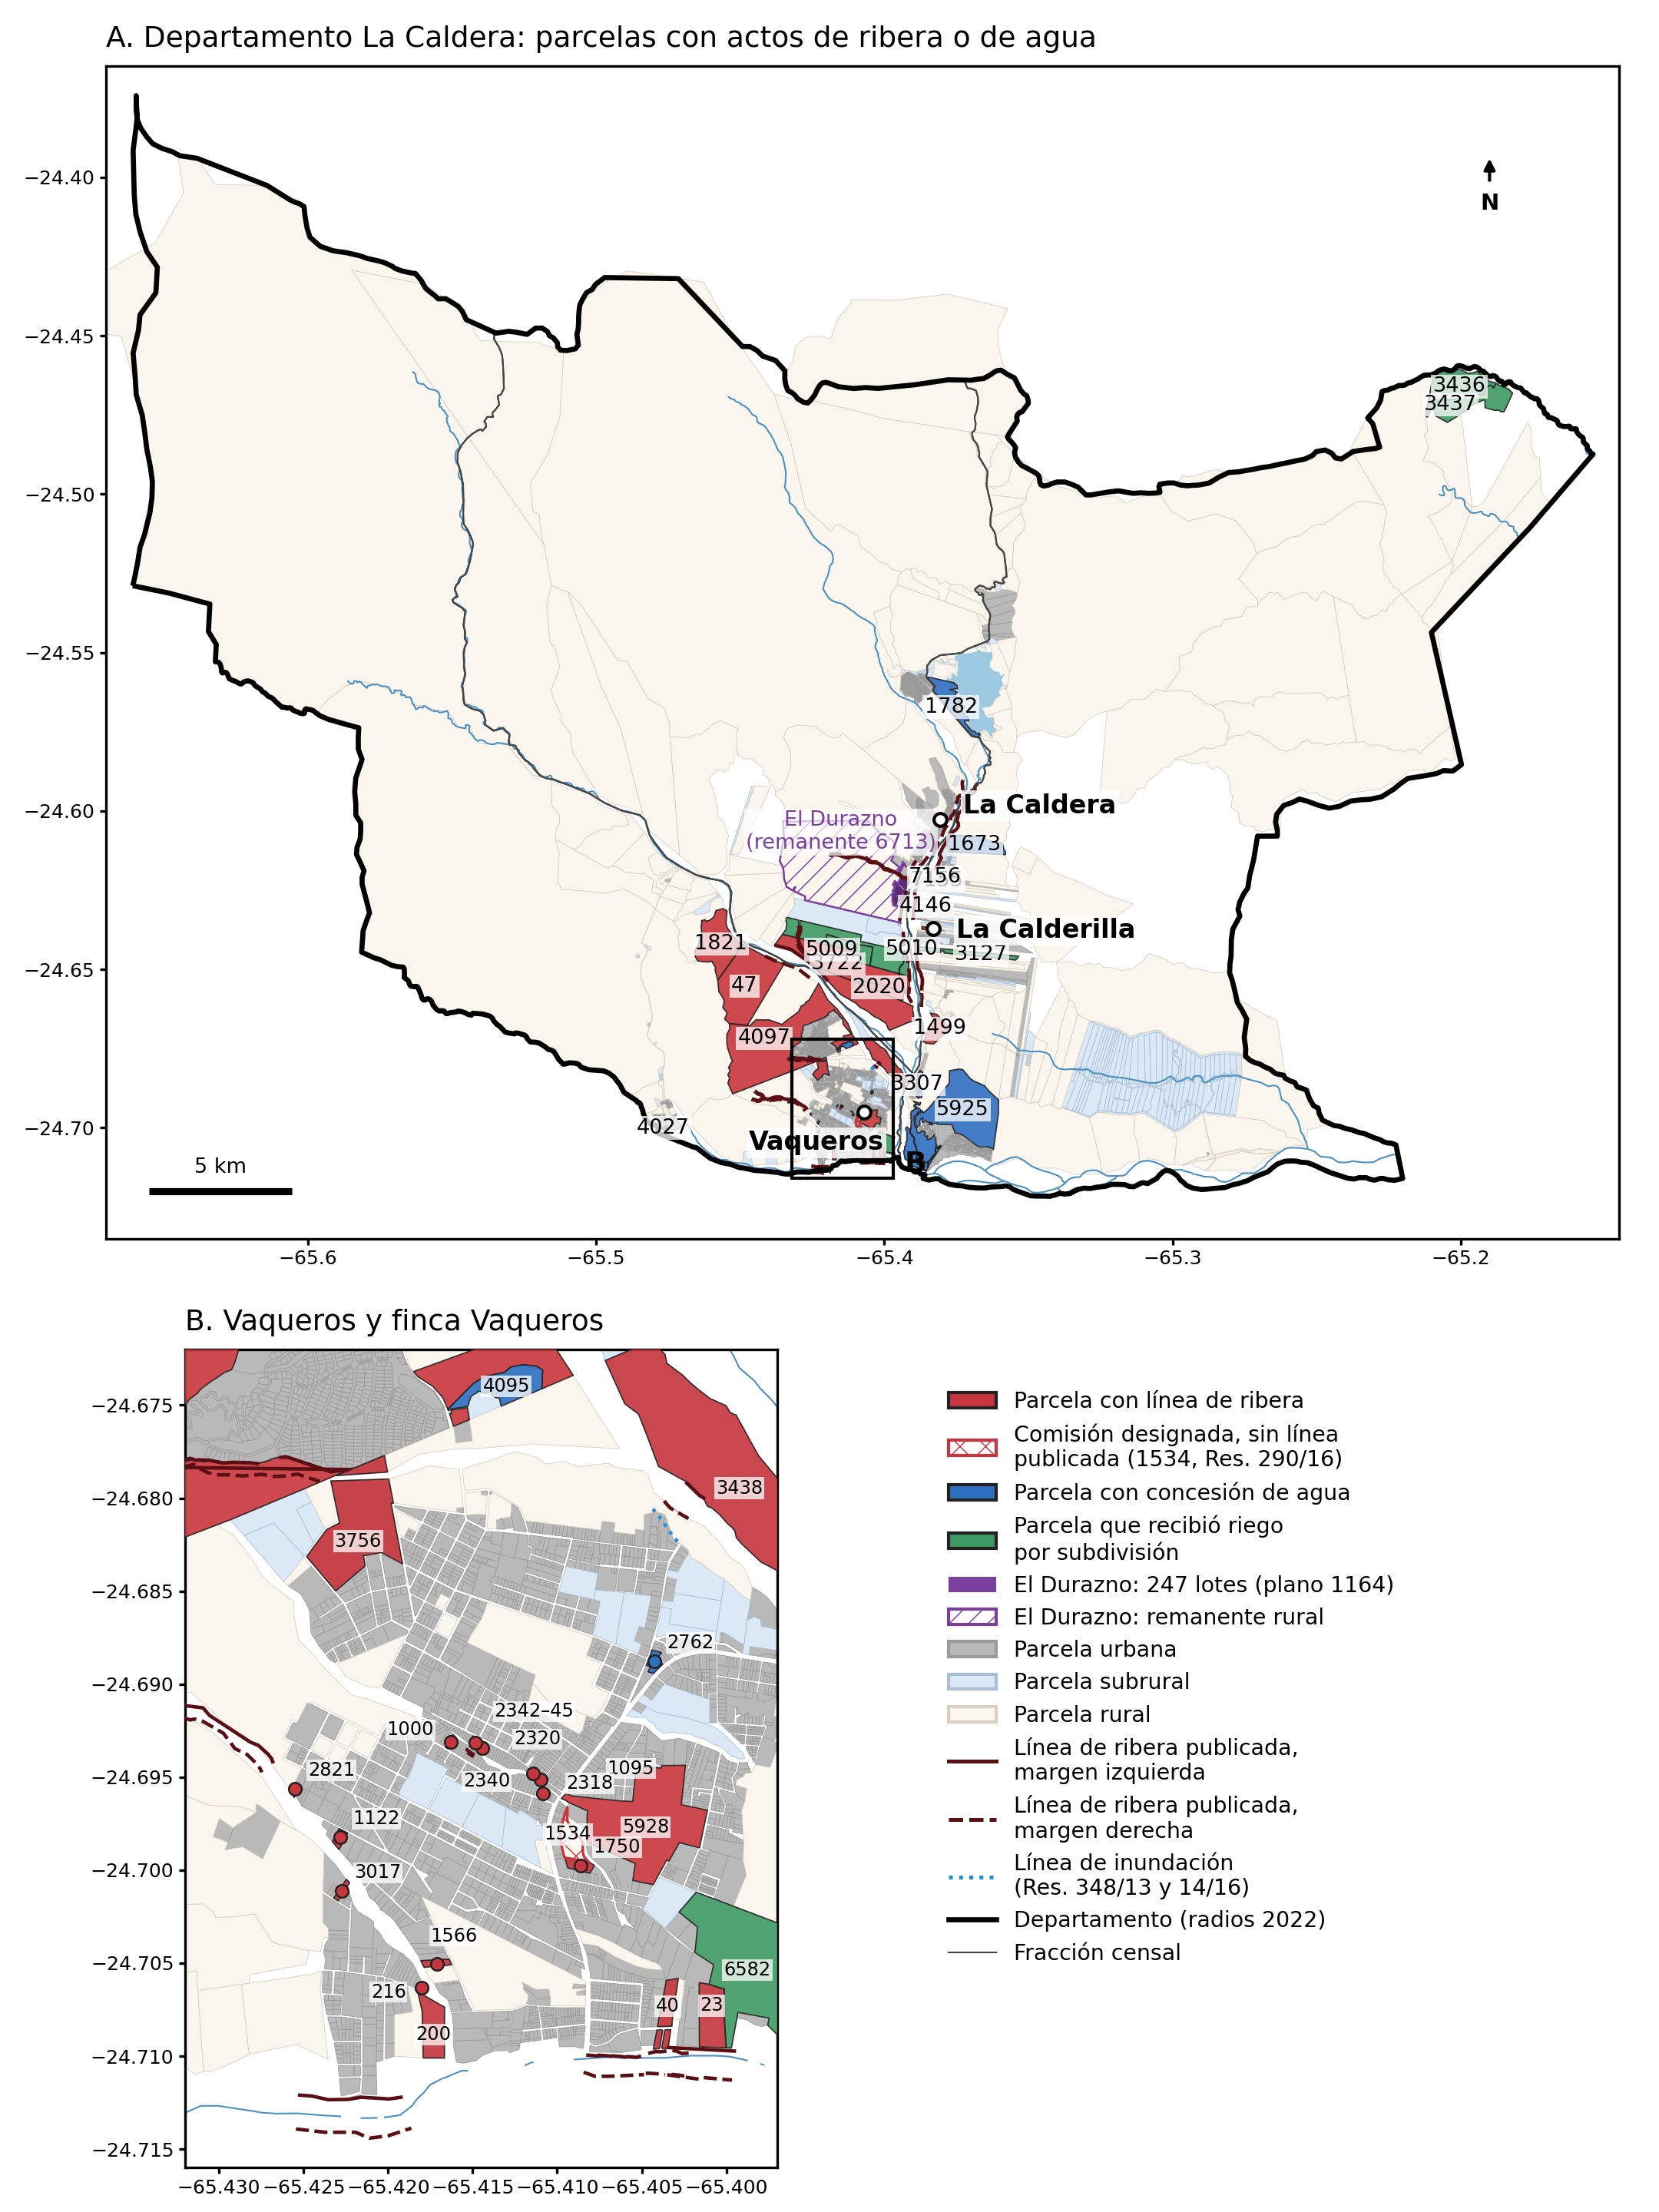
\includegraphics[width=\textwidth,height=0.84\textheight,keepaspectratio]{fig-catastro-ribera.png}
\caption[Las parcelas de las líneas de ribera y de las concesiones de agua]{\textbf{Las parcelas de las líneas de ribera y de las concesiones de agua.} A: el departamento, con las parcelas sobre las que recayó una determinación o comisión de línea de ribera (rojo), una concesión de agua (azul) o una asignación de riego por subdivisión (verde), y los 247 lotes y el remanente del plano de El Durazno (violeta). B: Vaqueros, donde los círculos marcan las parcelas menores de dos hectáreas; en trazo oscuro, las líneas de ribera cuyas coordenadas publicó el Boletín (Resoluciones 80/14, 201/13, 414/16, 144/17, 14/16 y 205 a 212/17), y en punteado celeste la línea de inundación de la 14/16. Los blancos dentro del departamento son sectores sin parcela en la capa. Elaboración propia con la capa «Catastro Urbano y Rural de la Provincia de Salta» de la Dirección General de Inmuebles (Geoportal IDESA, descargada en septiembre de 2026; cartografía orientativa según el propio organismo), la cartografía de radios del Censo 2022 (INDEC) y las coordenadas publicadas en los edictos. Coordenadas convertidas desde POSGAR 94, faja 3. Elaboración propia. \textbf{El script que dibuja esta lámina no está todavía en el repositorio} \texttt{mapas\_caldera}: \texttt{scripts/mapa\_ribera.py} dibuja la lámina \ref{fig:riberaedictos}, no ésta (apéndice \ref{cap:fuentes}).}\label{fig:catastro}
\end{figure}


{\small
\setlength{\LTpre}{0.6em}\setlength{\LTpost}{1.2em}
\begin{longtable}{@{}p{1.5cm}p{3.7cm}p{1.9cm}p{4.8cm}@{}}
\toprule
\textbf{Catastro} & \textbf{Acto del libro} & \textbf{Superficie} & \textbf{Categoría y finca} \\
\midrule
\endhead
\multicolumn{4}{@{}l}{\textit{Líneas de ribera sobre lotes urbanos}} \\
216 & Res.\ 009/12, 57/2025 y 130/2025 & 0,14 ha & Urbano, Vaqueros \\
3017 & Res.\ 125/2021 y 107/2022 & 0,38 ha & Urbano, Vaqueros \\
1566 & Res.\ 23/2021 & 0,64 ha & Urbano, Vaqueros \\
1122 & Res.\ 56/2025 & 0,58 ha & Urbano, Vaqueros \\
2342--2345 & Res.\ 205 y 210--212/17 & 0,08--0,09 ha c/u & Urbano, planos 362 y 1230 \\
2318 y 2320 & Res.\ 51 y 167/2022 & 0,05 ha c/u & Urbano, Vaqueros \\
1000, 1095, 1750, 2340 & Res.\ 209 y 206/2022, 182/2021, 61/2024 & 0,10--0,96 ha & Urbano, Vaqueros \\
2821 & Res.\ 75/2020 (con zona inundable) & 0,24 ha & Urbano, Vaqueros \\
4027 & Res.\ 94/12 (advertencia de no construir) & 1,35 ha & \textbf{Urbano} \\
3756 & Res.\ 292/13 y 142/2025 & 23,6 ha & \textbf{Urbano} (en 2013, «fracción 48») \\
4146 & Res.\ 291/16, 279/17, 108/2025 & 5,05 ha & Urbano, La Calderilla \\
\multicolumn{4}{@{}l}{\textit{Líneas de ribera sobre fincas}} \\
40 & Res.\ 147/16, 414/16, 144/17 & 2,94 ha & Urbano, sección B \\
200 & Res.\ 338/16 & 4,61 ha & Subrural, finca Cerro de Buena Vista \\
23 & Res.\ 198/15 y 322/15 & 5,64 ha & Subrural, finca Vaqueros \\
4097 & Res.\ 360/16, 304/17, 44/2021, 94/2022 & \textbf{901 ha} & Rural, finca Vaqueros (plano 860) \\
3722 & Res.\ 74/15, 293/15, 154/16 & 320 ha & Rural, finca Wierna \\
2020 & Res.\ 428/15 & 39 ha & Rural, finca Wierna \\
1821 & Res.\ 181/2020 & 215 ha & Rural, finca Huerta Vieja \\
47 & Res.\ 174/2021 & 380 ha & Rural, La Mesada, fracción B \\
3438 & Res.\ 319/15, 360/16, 304/17 & 78 ha & Subrural \\
5928 & Res.\ 327/19 & 30 ha & Rural, finca Vaqueros \\
1499 & Res.\ 282/16 & 51 ha & Rural, finca San Jorge \\
\multicolumn{4}{@{}l}{\textit{Concesiones de agua}} \\
4095 & Las Vertientes (2017) & 7,0 ha & Subrural, finca Vaqueros (plano 860, lindero de la 4097) \\
1782 & Skru S.A.\ (2019) & 94 ha & Rural, finca Campo Alegre \\
5925 & El Chalchal S.R.L.\ y otro (2025) & 573 ha & Rural, finca Chaguadero y San José \\
3307 & Valle Hermoso S.R.L.\ (2019) & 10,9 ha & Urbano \\
1673 & Arzobispado de Salta (2024) & 104 ha & Rural, finca Orco Huasi \\
6582 & Riego del catastro 2907 (2021) & 32 ha & Rural, finca \textbf{Sausal o Curuzú} \\
5009 y 5010 & Riego del catastro 3721 (2018, 2022) & 62 y 238 ha & Rurales, finca Wierna, linderas \\
3436 y 3437 & Riego del catastro 169 (2022) & 182 y 169 ha & Rurales, fincas Loma Pelada y Antilla, linderas \\
7155 y 7156 & Riego de los catastros 84, 2264 y 2932 (2023) & 2,0 y 10,8 ha & Subrurales, finca La Calderilla \\
3127 & Riego del catastro 38 (2005) & 49 ha & Rural, finca San Antonio \\
2762 & Vivero (2023) & 0,81 ha & Urbano \\
\bottomrule
\end{longtable}
}

\begin{cautela}
La capa confirma lo que los edictos sugerían y le pone medida. Las líneas de ribera del arroyo Vaqueros y del Chaile posteriores a 2019 no recaen sobre fincas sino sobre \textbf{lotes urbanos de entre quinientos metros cuadrados y una hectárea}. El inmueble de la matrícula 216, con una línea de 2012, otra de marzo de 2025 y la rectificación de junio, mide mil cuatrocientos metros cuadrados. La determinación de la ribera, que en 2013 se hacía para fracciones rurales, es hoy un trámite de lote.

Tres casos merecen registro aparte. La matrícula 4027, cuyo propietario fue advertido por escrito en 2012 de que no construyera viviendas cerca del río Castellanos, figura hoy como parcela \textbf{urbana}. La 3756, que en 2013 era la «fracción 48» de Finca Vaqueros, figura como urbana de veintitrés hectáreas cuando en 2025 se aprueba su línea. Y la 6582, a la que en 2021 se pasó el riego de la 2907, es la finca \textbf{«Sausal o Curuzú»}, la misma que el juez mandó deslindar en 1921 junto con Cerro de Buena Vista (capítulo \ref{cap:loteo}); la matrícula 200, con comisión de 2016 sobre el río Vaqueros, lleva el nombre de esta última.

La capa también muestra lo que ya no está. No figuran las matrículas de origen de los loteos y de las subdivisiones ---3616 (La Misión III), 3709 (Chacras del Gallinato), 3989 (Las Vertientes), 1905 y 1713 (Cerro de Buena Vista), 4366 y 6558 (El Durazno), 4953 (Finca Vaqueros), 3721, 2907, 126, 169 y 38---: se dieron de baja al dividirse. Las cadenas que los edictos de riego describen se verifican en el mapa: las matrículas 5009 y 5010 son linderas y salen de la 3721; las 3436 y 3437, de la 169; la 6582 sustituye a la 2907. La 4095 de Las Vertientes y la 4097 comparten el plano 860 y lindan. Una sola discordancia: el catastro 2264, que el edicto de 2023 da por anulado, sigue en la capa.

Por último, una conjetura que la capa descarta: los catastros 5925 y 5928, de numeración casi contigua, no son vecinos; los separan novecientos metros y dos planos distintos.
\end{cautela}

\section{El artículo 172, que ninguna fuente anterior había traído}

El edicto de 2013 transcribe el texto de una norma que cambia el peso de todo este capítulo.

\begin{ficha}{Art.\ 172 del Código de Aguas (Ley 7017) --- texto transcripto en el edicto}
``Zonas inundables. La Autoridad de Aplicación, para las zonas ribereñas determinará los sectores que puedan ser afectados por inundaciones, \textbf{en los cuales no se permitirá la instalación de asentamientos poblacionales} o fijación de obstáculos que puedan afectar el curso de las aguas. \textbf{Las nuevas construcciones o plantaciones que se efectúen en zonas ribereñas deberán ser autorizadas previamente por la Autoridad de Aplicación}, debiéndose proyectar y ejecutar las obras necesarias para prevenir el riesgo de inundación.''
\end{ficha}

\begin{cautela}
Léase con cuidado, porque es la norma más exigente que este libro encontró y conviene no forzarla.

Dice dos cosas distintas. La primera es una \textbf{prohibición}: en los sectores que la Autoridad determine como afectables por inundaciones no se permite la instalación de asentamientos poblacionales. La segunda es un \textbf{requisito de autorización previa}: toda nueva construcción en zona ribereña necesita permiso de la Autoridad de Aplicación, y deben proyectarse y ejecutarse las obras que prevengan el riesgo.

Ambas dependen de que exista determinación previa. La prohibición opera sobre ``los sectores que'' la Autoridad haya determinado; el permiso opera sobre ``zonas ribereñas'', que la línea de ribera define. En el río La Caldera, matrícula 1590, esa determinación existe desde noviembre de 2013 e incluye la zona inundable. En los arroyos El Durazno y Guaranguay, matrícula 4366, existe línea de ribera desde diciembre de 2014; si incluyó zona inundable es lo que no se sabe.

De ahí las dos preguntas que este capítulo debe formular y no responder. \textbf{Primera:} ¿la Resolución 383/14 determinó zona inundable sobre los arroyos, y qué superficie del loteo El Durazno queda dentro? \textbf{Segunda:} las construcciones levantadas en zona ribereña de esos arroyos, ¿contaron con la autorización previa que exige el artículo 172, y con las obras de prevención que la norma manda proyectar y ejecutar?

Nada permite afirmar que no las hayan tenido. Afirma que la norma las exigía, que el organismo competente es el mismo que intervino a fojas 59 del expediente del loteo, y que la respuesta está en ese expediente y en el de la determinación. No es una hipótesis: es un permiso que se otorgó o no se otorgó, y consta o no consta.
\end{cautela}

Una precisión sobre el error de numeración, que este edicto obliga a reformular. El de 2013 también cita ``Dcto.\ Nº 1898/02, art.\ 10'', igual que el de julio de 2014 ---el de la Resolución 185/14--- y el de 2015. El de 2019 y el de julio de 2025 citan 1989/02, que es el correcto; el de abril de 2025 sobre el arroyo Vaqueros vuelve a decir 1898/02. Y antes de la serie, el edicto de mayo de 2012 sobre Chacras del Gallinato, firmado por otro funcionario, también cita correctamente el 1989/02: la transposición no viene del origen del régimen.

No fue entonces un desliz aislado: fue un \textbf{error de plantilla que atraviesa toda la serie}. Las tablas de este mismo capítulo lo registran en 2013, 2014 y 2015, en las Resoluciones 282/16, 389/16 y 279/17 y en la serie del arroyo Chaile de 2021 a 2024; el edicto de 2019 sobre el río Bermejo y el de julio de 2025 citan el número correcto, y el de abril de 2025 vuelve al error. Las dos versiones conviven desde 2013. Es el segundo error de plantilla que este libro documenta --- el primero es el municipio de Rivadavia Banda Sur en el Plan de Desarrollo Urbano Ambiental --- y ambos comparten el mismo mecanismo: un texto que se reutiliza y que nadie relee.

La pregunta que este capítulo había dejado abierta --- si la Ley 7017 fija, como su análoga cordobesa, un plazo para levantar los planos de zonas inundables --- ya tiene respuesta. Obtenido el texto completo del Código de Aguas y de su reglamentación: \textbf{no lo fija}.

El artículo 194 del código cordobés, de 1973, ordena a la Autoridad levantar esos planos ``dentro de los diez años''. El artículo 172 salteño, de 1998, reproduce el resto del contenido --- la prohibición de asentamientos, la autorización previa de construcciones --- y \textbf{omite el plazo}. La obligación de determinar los sectores inundables existe; el término para cumplirla, no.

Es una diferencia de una línea y tiene consecuencia práctica: sin plazo no hay incumplimiento de plazo. La determinación de zonas inundables en el departamento La Caldera podía hacerse en 1999 o en 2030 sin que ninguna fecha se venciera.

\section{Y el certificado no es un trámite: es un recaudo indispensable}

La reglamentación del Código de Aguas contiene, en el artículo que reglamenta el 172, la norma que la presentación del COHIFE mencionaba sin citar.

\begin{ficha}{Art.\ 172º de la reglamentación --- texto}
``La Autoridad de Aplicación es el organismo competente para expedir las certificaciones de \textbf{`no inundabilidad'}, que constituyen \textbf{un recaudo indispensable para todo asentamiento poblacional, urbanización, o plantación en zona ribereña}. Ello, previo cobro a los interesados de un arancel, que fijará para cada caso la Autoridad de Aplicación.''
\end{ficha}

``Recaudo indispensable''. No es una constancia recomendable ni un requisito que la autoridad pueda dispensar: la norma lo califica de indispensable, y lo hace \textbf{para todo asentamiento poblacional o urbanización en zona ribereña}, sin distinguir tamaño, época ni jurisdicción.

El loteo El Durazno es una urbanización. Está atravesado por dos arroyos con línea de ribera determinada desde diciembre de 2014. El organismo competente para expedir el certificado es el mismo que intervino a fojas 59 del expediente de aprobación de su plano, en 2021.

La pregunta que este capítulo formuló hace unas páginas queda ahora apoyada en el texto de una norma y no en una presentación: \textbf{¿se expidió el certificado de no inundabilidad?} Y como el propio artículo prevé el cobro de un arancel, hay además un rastro contable: un certificado expedido dejó un pago.

\section{Dos artículos vecinos que el capítulo necesitaba}

\begin{ficha}{Arts.\ 171 y 173 de la Ley 7017 --- texto}
\textbf{Art.\ 171 --- Información previa.} ``Previo al otorgamiento, por parte de la autoridad competente, de permisos o concesiones de uso de cauces, márgenes o \textbf{extracción de áridos}, la Autoridad de Aplicación evaluará si el permiso o concesión afectará desfavorablemente las riberas o el flujo de aguas, si así fuera desaconsejará el otorgamiento del permiso o concesión, o se exigirá la construcción de las obras necesarias y la aplicación de las técnicas de operación adecuadas para prevenir los peligros y los daños.''

\textbf{Art.\ 173 --- Penalidades.} Las infracciones al artículo 172 se sancionan con multa y sanciones conminatorias. ``Sin perjuicio de ello la Autoridad de Aplicación podrá \textbf{ordenar la demolición de las obras o la destrucción de los obstáculos} o demolerlos o destruirlos por cuenta del infractor.''
\end{ficha}

El artículo 171 conecta con lo que, según la prensa, se ordenó reparar en la ejecución en noviembre de 2025 ---acto que la lista de actuaciones consultada no registra---: el daño causado por la extracción irregular de áridos. La norma exigía, desde antes, una evaluación previa de impacto sobre riberas y flujo para cada permiso de extracción. Si esas evaluaciones existen, están en la Autoridad de Aplicación.

El artículo 173 es el que más pesa, y conviene enunciarlo con cuidado. \textbf{La provincia tiene, desde 1998, la potestad de ordenar la demolición de obras levantadas en violación del artículo 172.} No es una facultad que este libro reclame ni recomiende --- se trata de viviendas habitadas por familias, y ninguna solución que pase por demolerlas sería una solución. Lo que corresponde registrar es de otro orden: la herramienta jurídica más severa del régimen hídrico provincial existía y no fue necesario discutirla, porque nunca se llegó al momento en que hubiera que decidir si aplicarla.

Cuándo se estuvo cerca de ese momento, y quién no lo advirtió, es la pregunta que atraviesa este capítulo desde su primera página.

\section{Hay rectificaciones en el departamento, y son recientes}

El capítulo \ref{cap:vaqueros} planteaba, sobre la base del mismo material, que existe un mecanismo de modificación de la línea de ribera a pedido de desarrolladores. La existencia del mecanismo quedó confirmada por el artículo 1º del Anexo I --- la determinación procede a solicitud de parte --- y por el artículo 126 in fine del Código de Aguas. Y ahora hay casos fechados en el propio departamento. El primero que se transcribe no es, en rigor, una rectificación sino una determinación demorada casi doce años; las rectificaciones son las que le siguen.

\begin{ficha}{Resolución Nº 000142/2025 --- B.O.\ Nº 22.007 y 22.008, 8 y 11 de agosto de 2025}
Expediente 0090034-160869/2013-0/4. Aprueba, el 30 de junio de 2025, la determinación de la línea de ribera realizada por la Comisión Técnica en ambas márgenes del \textbf{arroyo Quintín}, a la latitud del \textbf{catastro 3756}. Puntos de vinculación a disposición en la sede. Autorizado a diligenciar la publicación: \textbf{Ing.\ Antonio Alejandro Forns}\index{Forns, Antonio Alejandro}. Firma la jefa del Programa Jurídico, Silvia F.\ Santamaría. Cita correctamente el Decreto 1989/02 y admite el recurso por correo electrónico. Edicto del 7 de julio de 2025.
\end{ficha}

\begin{cautela}
Es la determinación que cierra la comisión de la Resolución 292/13: el mismo expediente, el mismo catastro y el mismo arroyo, \textbf{casi doce años después}. En el camino el número del expediente migró al formato nuevo y cambiaron el asesor y el formato del edicto. Lo que no cambió es un nombre: el ingeniero Forns, que integró la comisión de 2013, es en 2025 quien está autorizado a diligenciar la publicación. El edicto no dice en representación de quién. En la Resolución 108/2025 la misma función la cumple otro ingeniero. Qué determinó la comisión en 2013 y qué se aprobó en 2025 ---si es la misma línea o una actualizada por la migración del cauce--- es lo que diría el expediente. \pendiente{expediente 0090034-160869/2013, con el informe de la comisión y los fundamentos de la Resolución 142/2025}
\end{cautela}

\begin{ficha}{Resolución Nº 000108/2025 --- B.O.\ Nº 21.962, 30/05 y 02/06/2025}
Expediente Nº 0090034-242142/2024-0. La Secretaría de Recursos Hídricos hace saber que por Resolución Nº 000108/2025 del \textbf{9 de mayo de 2025} \textbf{se rectificó en su parte pertinente la determinación de la línea de ribera aprobada por las Resoluciones Nº 279/17 y 306/19}, realizada por la Comisión Técnica en ambas márgenes del \textbf{río La Caldera}, en la zona de la \textbf{Matrícula Nº 4146} del departamento La Caldera.

Puntos de vinculación a disposición en la sede. Autorizado a diligenciar: \textbf{Ing.\ Jesús E.\ Flores}. Firma: Dra.\ Silvia F.\ Santamaría\index{Santamaría, Silvia F.}, Jefa de Programa Jurídico. Apelable ante el Tribunal de Aguas (Decreto 1989/02, art.\ 10) en diez días hábiles administrativos.
\end{ficha}

\begin{cautela}
Conviene separar tres asuntos.

\textbf{Primera: la serie del río La Caldera es larga.} La comisión se designó por Resolución 291/16 (véase el apartado sobre 2016 y 2017); la línea de ribera se determinó por Resolución 279/17, se volvió a tratar por Resolución 306/19 y se rectificó por Resolución 108/2025. Tres actos en ocho años sobre el mismo curso, en un departamento donde entre medio ocurrieron dos aluviones y una condena judicial.

\textbf{Segunda: aparece una matrícula nueva.} La 4146. El libro venía siguiendo la 4366 --- zona de la determinación de 2014 sobre los arroyos --- y la 6.558 --- inmueble del loteo El Durazno. Tres matrículas del mismo departamento, sobre las que el Estado fijó o rectificó líneas de ribera y aprobó un fraccionamiento. Establecer su relación es, otra vez, el antecedente dominial que falta.

\textbf{Tercera: qué se rectificó y por qué.} El edicto dice ``en su parte pertinente'' y no dice más. Puede tratarse de una corrección técnica menor, de una actualización por migración del cauce --- que el artículo 7 del Anexo I contempla expresamente --- o de una modificación de alcance. Este libro \textbf{no lo sabe} y no debe elegir entre las tres. Lo que corresponde es pedir el expediente 0090034-242142/2024-0, que es corto y está identificado.
\end{cautela}

Queda resuelta, además, la discrepancia que este capítulo había señalado entre los decretos 1989/02 y 1898/02. El correcto es \textbf{1989/02}: así lo cita la presentación oficial, así lo cita el edicto del río Bermejo y así lo cita el edicto de julio de 2025; el de abril de ese año sobre el arroyo Vaqueros, en cambio, repite el error. La mención a ``1898/02'' en el edicto de la Resolución 383/14 es una transposición de dígitos \textbf{en el propio edicto}.

Es un error menor y sin consecuencia jurídica, pero se repite en edictos de 2013 a 2017 y de 2021 a 2025, falta en otros de esos mismos años ---y en los de 2019 y julio de 2025---, y reaparece en el de abril de 2025: es un defecto de plantilla que convive con la versión corregida. Conviene registrarlo por lo que dice del control de calidad de las publicaciones: durante años, el instrumento que informaba a los vecinos bajo qué norma podían apelar citó mal el número de esa norma.

Se obtuvo el texto del artículo 126 y un edicto de 2019 del mismo organismo que permite ver el procedimiento completo. Ambos corrigen datos que este apartado había tomado de un resumen intermedio, antes de identificar la presentación de Torres.

\begin{ficha}{Art.\ 126 del Código de Aguas (Ley 7017) --- texto}
La Autoridad de Aplicación determina la línea de los cursos naturales \textbf{conforme al criterio del artículo 2.577 del Código Civil} y según el procedimiento técnico que fije la reglamentación, \textbf{dando intervención en la operación a los interesados}. Las cuotas determinantes se anotan en el Libro de Catastro que prevé el Código. Y en su última oración: \textbf{``La Autoridad de Aplicación podrá rectificar la línea de ribera cuando el cambio de las circunstancias lo haga necesario.''}
\end{ficha}

\begin{cautela}
Dos observaciones sobre este artículo.

La primera es una cuestión abierta que este libro señala sin resolver. El artículo remite al \textbf{artículo 2.577 del Código Civil} de Vélez, cuerpo derogado en agosto de 2015 y reemplazado por el Código Civil y Comercial, cuyo artículo 235 delimita el río por la línea de ribera que fija \textbf{el promedio de las máximas crecidas ordinarias}. Qué criterio rige hoy en Salta --- si la remisión debe entenderse dinámica hacia el texto vigente, o si subsiste el criterio del código derogado --- es una pregunta jurídica que excede a este libro y que corresponde formular a la Autoridad de Aplicación. La determinación de 2014 que aquí importa es anterior a esa derogación.

La segunda es que la \textbf{rectificación está prevista en la ley}. La presentación de Torres describe que proyectos privados solicitan corrimientos de la línea; el artículo 126 in fine muestra que la potestad de rectificar existe, aunque el texto la atribuye a la Autoridad ``cuando el cambio de las circunstancias lo haga necesario'' y no a pedido de un desarrollador. Que exista la puerta no prueba quién la usa ni para qué. Los expedientes de rectificación del departamento siguen siendo el documento que lo establecería.
\end{cautela}

\section{Once años después, el edicto sigue siendo el mismo}

El núcleo de este capítulo ---la serie de veinticinco actos--- ocurrió entre 2013 y 2015. Queda la pregunta de si aquella
forma de publicar era propia de esos años, de ese departamento o de aquel firmante. Un edicto de
2025 la contesta.

\begin{ficha}{Boletín Oficial Nº 21.987, 10 y 11 de julio de 2025}
Expediente 0090034-194687/2024-0. La Secretaría de Recursos Hídricos hace saber que por
\textbf{Resolución Nº 000111/2025} del 30 de junio de 2025 se aprobó la determinación de línea
de ribera en ambas márgenes del \textbf{río Ancho}, a la latitud del catastro 9.226 del
\textbf{departamento Cerrillos}, «\textit{cuyos puntos de vinculación \textbf{se encuentran a
disposición de los interesados en la sede} de la Secretaría de Recursos Hídricos}».

Firma la \textbf{Dra.\ Silvia F.\ Santamaría}\index{Santamaría, Silvia F.}, Jefa de Programa
Jurídico. Arancel: \textbf{once mil novecientos pesos}.
\end{ficha}

\textbf{Es la misma fórmula, palabra por palabra, que la Resolución 383/14.} Otro departamento,
otra cuenca, otro firmante, once años después.

La fecha de la resolución es la que da el edicto, y no encaja en la numeración de la
Secretaría: la 108/2025 es del 9 de mayo, la 130/2025 del 9 de junio y la 142/2025 del 30 de
junio, el mismo día que el edicto atribuye a la 111/2025. \pendiente{fecha de la Resolución 111/2025 en el registro de la Secretaría de Recursos Hídricos}

\begin{cautela}
Este hallazgo corta en dos direcciones y las dos importan.

\textbf{Debilita cualquier lectura particular.} No hubo una decisión tomada sobre El Durazno y
Guaranguay: hay \textbf{una forma de redactar edictos} que el organismo viene usando, que
alterna con la otra ---la que publica coordenadas--- y que sigue vigente. Este libro nunca
afirmó que la omisión fuera deliberada; ahora tiene además una razón positiva para no
afirmarlo.

\textbf{Y refuerza la tesis estructural.} Lo que el capítulo \ref{cap:opacidad} describe no es
una conducta sino un criterio disponible: dos plantillas, ninguna norma que mande elegir una, y
nadie obligado a explicar la elección. \textbf{Que once años después convivan las dos es la
prueba más limpia de que no hay criterio escrito.}

\textbf{Lo que este edicto no prueba}, por sí solo, es cómo se publicaron las determinaciones de La Caldera entre 2016 y 2024; las series del Chaile, del Wierna y del Vaqueros que este capítulo reúne muestran que desde 2019 ninguna publica sus coordenadas. En 2025 la fórmula sí se repitió en el departamento ---la Resolución 56/2025 sobre el arroyo Vaqueros y la 108/2025 sobre el río La Caldera remiten sus puntos a la sede---, pero el apéndice \ref{cap:pedidos} pide las resoluciones 279/17 y 306/19, que son las que faltan para cerrar la serie del río La Caldera.
\end{cautela}

\subsection*{Y en 2026, otra vez}

No es un caso aislado de 2025. Nueve meses después vuelve a ocurrir, en un tercer departamento.

\begin{ficha}{Boletín Oficial Nº 22.160, 1 y 6 de abril de 2026}
Expediente 0090034-130747/2025-0. La \textbf{Subsecretaría} de Recursos Hídricos hace saber que
por \textbf{Resolución Nº 000016/2026} del 4 de marzo de 2026 se aprobó la determinación de
línea de ribera en ambas márgenes del \textbf{río Calchaquí}, en zona de la matrícula 538 del
\textbf{departamento San Carlos}, «\textit{cuyos puntos de vinculación se encuentran a
disposición de los interesados en la sede de la Secretaría de Recursos Hídricos}».

Firma la \textbf{Dra.\ Silvia F.\ Santamaría}, ahora \textbf{Directora de la Dirección Legal y
Técnica}. Arancel: \textbf{diecisiete mil cuarenta pesos}.
\end{ficha}

\textbf{Tres departamentos, tres cuencas, tres años, la misma frase.} Cerrillos en 2025, San
Carlos en 2026, La Caldera en 2014. Lo que este capítulo documentó como un episodio es
\textbf{la forma habitual de un organismo}.

\begin{cautela}
\textbf{Y este edicto resuelve un pedido del apéndice \ref{cap:pedidos}.}

Ese apéndice preguntaba si el organismo hídrico había cambiado de rango entre 2024 y 2025. La
respuesta está en el encabezado de los dos edictos: en julio de 2025 firma la
\textbf{Secretaría} de Recursos Hídricos; en marzo de 2026, la \textbf{Subsecretaría}.
\textbf{El organismo bajó de rango entre ambas fechas.} La ventana se acorta: el Decreto 52/26, publicado el 13 de febrero de 2026, designa al Ing.\ Julio Mauricio \textbf{Romero Leal}\index{Romero Leal, Mauricio} \textbf{Subsecretario} de Recursos Hídricos. Es el mismo funcionario que en 2022 y 2023 figuraba como \textbf{secretario} del área (capítulo \ref{cap:amparo}): el organismo perdió rango y su titular volvió a él con el cargo nuevo. El cambio es parte del reordenamiento de fines de 2025. La \textbf{Ley 8.511} (B.O.\ del 26/11/2025) suprimió el Ministerio de Infraestructura, pasó las tierras fiscales a la Jefatura de Gabinete (capítulo \ref{cap:tierrafiscal}) y fijó un tope de treinta secretarías de Estado (art.\ 30). En la letra de la ley, el uso y aprovechamiento de los recursos hídricos corresponde al Ministerio de \textbf{Producción y Minería}, junto con el contralor de las explotaciones mineras, la autoridad ambiental y el ordenamiento territorial (art.\ 25, incs.\ 7, 9, 13 y 14). Pero la estructura de ese ministerio, aprobada por la Decisión Administrativa 565/25 con vigencia al 15 de diciembre de 2025 (B.O.\ Nº 22.100 del 30/12/2025; lámina \ref{lam:da565}), \textbf{no incluye al organismo hídrico}. Su organigrama tiene cuatro secretarías ---Ambiente y Desarrollo Sustentable, Industria y Comercio, Minería y Desarrollo Agropecuario--- y ninguna unidad de recursos hídricos en ningún nivel. La Subsecretaría quedó en la \textbf{Jefatura de Gabinete de Ministros}, a la que la misma ley asigna las obras de aprovechamiento de cuencas y recursos hídricos (art.\ 19, inc.\ 16): el Decreto 52/26, del 10 de febrero de 2026 (B.O.\ Nº 22.131), que designa a Romero Leal, lleva ese encabezado y lo refrenda el jefe de Gabinete. Lo que el organigrama sí muestra es que el ambiente conservó el rango de Secretaría y que ambiente y minería quedaron como secretarías hermanas bajo el mismo ministro. \textbf{El agua, en cambio, perdió rango y quedó fuera del ministerio que la ley nombra competente.} Quedó, en cambio, bajo la misma jefatura y el mismo funcionario que las tierras fiscales, el catastro y las obras públicas (capítulo \ref{cap:tierrafiscal}). \textbf{Los tres circuitos que este libro sigue para cada loteo ---el dominio, el plano y la línea de ribera--- dependen desde diciembre de 2025 de una sola oficina.} La estructura de esa jefatura, aprobada por la Decisión Administrativa 569/25 (23/12/2025, con vigencia al 15 de diciembre; B.O.\ Nº 22.100 del 30/12/2025), tiene seis secretarías ---Obras Públicas, Coordinación Interministerial, Interior, Prensa y Comunicación, Tierra y Bienes del Estado y Relaciones Internacionales---, y la Dirección General de Inmuebles depende directamente del jefe de Gabinete. \textbf{La Subsecretaría de Recursos Hídricos no depende de él sino de la Secretaría de Obras Públicas}: el organismo que determina las líneas de ribera quedó un escalón por debajo del que proyecta y contrata las obras, junto a sus direcciones de obras municipales y de infraestructura social y productiva. La Secretaría \textbf{del Interior}, por su parte, tiene a su cargo las relaciones con los municipios a través de una Subsecretaría de Asuntos Municipales. Su anexo nombra a los responsables del área hídrica, y dos ya aparecieron en este libro. El coordinador de la Subsecretaría es \textbf{David Le Favi}\index{Le Favi, David}, que en 2023, como director de Fiscalización y Control, firmó la nota a Fiscalía de Estado analizada en el capítulo \ref{cap:amparo}. El director general de Cuencas y Política Hídrica es \textbf{Jorge Genaro Torres}\index{Torres, Jorge G.}, con toda probabilidad el geólogo Jorge G.\ Torres de este capítulo: el autor de la presentación sobre línea de ribera y el integrante de las comisiones de 2014 y 2015. El director general de Concesiones Hídricas es Leandro Bruno.

Dos lecturas se siguen de ese cambio.

\textbf{La primera es de capacidad.} El capítulo \ref{cap:amparo} documenta que en la audiencia
de febrero de 2026 la propia Subsecretaría alegó falta de capacidad operativa. Que esa
alegación provenga de un organismo que acababa de perder rango ---y con él, presumiblemente,
presupuesto y planta--- no la vuelve más ni menos atendible, pero la ubica.

\textbf{La segunda es de plantilla.} El edicto lo emite la Subsecretaría y, sin embargo, ordena
presentar el recurso «ante la Secretaría de Recursos Hídricos». \textbf{El formulario no se
actualizó.} Es el mismo fenómeno que el error del «Dcto.\ 1898/02» que este capítulo documentó
entre 2013 y 2025: un texto que se arrastra de un edicto al siguiente sin que nadie lo lea.
\end{cautela}

\lamina{lam-da565-cabecera.jpg}{lam:da565} {Estructura del Ministerio de Producción y Minería desde el 15 de diciembre de 2025} {\textbf{Anexo I de la Decisión Administrativa 565/25, cabecera.} Bajo el ministro, cuatro secretarías: Ambiente y Desarrollo Sustentable, Industria y Comercio, Minería y Desarrollo Agropecuario. No hay unidad de recursos hídricos en ningún nivel del organigrama.} {Boletín Oficial de Salta Nº 22.100, 30/12/2025; anexo SA100052284, folio 3. Firmas del ministro José Ignacio Lupión y del coordinador administrativo Nicolás Demitrópulos. Escaneo en escala de grises, sin otras alteraciones.}

\textbf{Tres detalles menores del edicto de julio de 2025}, que conviene registrar porque cada uno cierra
algo que este capítulo dejó abierto.

\textbf{El número del decreto está bien citado} en este edicto, a diferencia del de abril del mismo año.

\textbf{El plazo se precisó.} Los diez días hábiles corren ahora «\textit{desde el día siguiente
de la última publicación}», y no «desde el día de la última publicación» como en 2013 y 2014. Es
un día de diferencia y es la clase de ajuste que sólo se hace cuando alguien lo discutió.

\textbf{Y la vía de recurso admite correo electrónico}: el edicto ofrece presentar el recurso en
Avenida Bolivia 4650 «\textit{o bien al mail}» de mesa de entradas de la Secretaría, que es una
casilla de Gmail. Este libro lo consigna sin ironía: \textbf{amplía el acceso de quien vive a
veinte kilómetros}, y es exactamente lo contrario de remitir las coordenadas a la sede. El mismo
organismo, en el mismo acto, acerca el recurso y aleja el dato.

\section{Cómo se ve un edicto de línea de ribera bien hecho}

El 7 y 8 de marzo de 2019, la misma Secretaría de Recursos Hídricos publicó un edicto sobre el río Bermejo, departamento Orán, expediente 0090034-289615/18. Sirve de patrón de comparación.

\begin{ficha}{Edicto del río Bermejo --- B.O.\ Nº 20.457, 7 y 8 de marzo de 2019}
Por \textbf{Resolución Nº 21 del 01/02/19 se aprobó la Comisión Técnica} que determinará la línea de ribera en ambas márgenes del río Bermejo, integrada por el \textbf{geólogo Enrique Chalabe} y el \textbf{ingeniero civil Marcelo Antonio Chalabe}. Se establece la zona: ambas márgenes del Bermejo en el área de la matrícula Nº 30.806 de Orán. \textbf{Método: geológico-geomorfológico.} Fundamento: Decreto Nº 1989/02, reglamentación del art.\ 126, Anexo I.

\textbf{``Los propietarios ribereños no podrán realizar ningún trabajo que implique la modificación actual de las márgenes en la zona objeto de la presente determinación.''}

Publicación por dos días. Los terceros interesados disponen de \textbf{quince días hábiles administrativos} desde la última publicación para presentar información, estudios, planos o cualquier dato que oriente la determinación, ante la sede de Avenida Bolivia 4.650. Firma: \textbf{Dra.\ Silvia Santamaría\index{Santamaría, Silvia F.}, Jefa de Programa Jurídico}.
\end{ficha}

\begin{cautela}
Este edicto obliga a corregir dos datos que el apartado anterior había tomado de un resumen intermedio, y a reformular la observación principal.

\textbf{Corrección primera:} la Comisión Técnica de este edicto tiene \textbf{dos} integrantes --- un geólogo y un ingeniero civil ---, cuando el artículo 3º del Anexo I del Decreto 1989/02 la conforma con \textbf{tres}: ingeniero hidráulico, geólogo y agrimensor. La diferencia no es un error de este libro sino un dato del expediente del Bermejo, y corresponde preguntar por ella, no darla por normal.

\textbf{Corrección segunda:} los quince días hábiles del edicto del Bermejo son para que terceros aporten estudios \textbf{durante} la determinación. Conviven con el plazo de diez días del artículo 10 del Anexo I, que corre para observar la línea propuesta y, cumplido sin oposición, la deja firme. Son dos plazos de dos momentos, no uno que desmiente al otro.

\textbf{Y la reformulación, que es más importante que las dos correcciones.} Lo que este edicto revela no es un plazo sino una \textbf{etapa}. Se publica \textbf{antes} de determinar: anuncia la comisión con nombre y apellido, declara el método que se empleará, delimita la zona, prohíbe cautelarmente a los ribereños modificar las márgenes mientras dure la operación, y abre quince días para que cualquiera aporte estudios. Eso es lo que el artículo 126 llama ``dar intervención en la operación a los interesados''.

El edicto de la Resolución 383/14 que este capítulo documenta pertenece al momento opuesto: comunica que la determinación \textbf{ya fue aprobada}, y remite las coordenadas a la sede. \textbf{No son el mismo acto y no deben compararse como si lo fueran.}

De donde surge una pregunta precisa: si el procedimiento incluye un edicto inicial como el del Bermejo, entonces para los arroyos El Durazno y Guaranguay \textbf{debió existir uno equivalente entre 2013 y 2014}, con los nombres de la comisión, el método elegido, la zona delimitada y la prohibición cautelar de modificar las márgenes. Si existió, hay que encontrarlo en el Boletín de esos años. Si no existió, la determinación se hizo sin la etapa participativa que la ley prevé. Las dos respuestas son informativas y ninguna está en poder de este libro.
\end{cautela}

\subsection*{Y el texto del Anexo I lo convierte en obligación}

El texto íntegro del Anexo I del Decreto 1.989/02 vuelve innecesaria la analogía con el edicto del Bermejo.

\begin{ficha}{Anexo I, artículos 2 y 4 --- texto literal}
\textbf{Art.\ 2.} «\textit{Partes interesadas. Serán partes interesadas todos los que se
consideren con un interés legítimo o en un derecho subjetivo y los organismos provinciales de
participación obligatoria.}»

\textbf{Art.\ 4.} «\textit{Notificación. La Comisión formada al efecto deberá notificar a
todas las partes interesadas que la Autoridad de Aplicación ha decidido realizar la
determinación de la línea de ribera correspondiente y además la Comisión \textbf{deberá
publicar en el Boletín Oficial por 2 (dos) días y en el medio gráfico de mayor difusión un
aviso de inicio de la determinación prevista}.}»
\end{ficha}

\textbf{El aviso de inicio no es una práctica: es un deber, con plazo y con soporte.} Y el
artículo 5 le da su razón de ser: las partes tienen quince días desde la notificación para
presentar «\textit{toda información, estudio, planos o cualquier otro dato}» que oriente a la
Comisión.

\begin{cautela}
De modo que la pregunta sobre el edicto inicial de El Durazno y Guaranguay tiene ahora consecuencia jurídica: \textbf{si no se publicó, la determinación se hizo omitiendo un acto que el Anexo I ordena en términos imperativos}. Este libro sigue sin saber cuál de las dos cosas ocurrió, pero ya no compara con otra cuenca: compara con el texto.
\end{cautela}

\subsection*{Y el aviso de inicio existe: está publicado en 2012}

Hasta acá la pregunta era si el aviso de inicio del artículo 4 se cumplía en la práctica. La
respuesta es que sí, y el ejemplo está en este mismo departamento, en el expediente contiguo.

\begin{ficha}{Boletín Oficial Nº 18.970, 13 de diciembre de 2012 --- O.P.\ Nº 100031653}
Referencia: \textbf{Expediente Nº 34-179.209/12}.

«La Secretaría de Recursos Hídricos hace saber que, por \textbf{Resolución Nº 322 del día
21/11/12 se aprobó la Comisión Técnica que determinará la línea de ribera} en ambas márgenes
del \textbf{Río La Caldera}, integrando dicha comisión los Sres.\ \textbf{Ing.\ Civil Felipe
Caro}, M.P.\ Nº 3024, el \textbf{Geólogo Marcelo Ramón Olañeta}, M.F.\ Nº 155, y el
\textbf{Topógrafo N.\ Félix Márquez}. Estableciéndose la determinación de
dicha línea, respecto del inmueble \textbf{Catastro Nº 3593, Fracción 17}, del Dpto.\ La
Caldera, como lugar donde la comisión técnica realizará dicha determinación,
\textbf{utilizándose el método de registro fotográfico y medición de caudales en base a datos
de precipitaciones. Decreto Nº 1989/02, art.\ 8 ap.\ 2 y 3}. Los propietarios ribereños en la
zona objeto de la presente determinación \textbf{no podrán realizar ningún trabajo que implique
la modificación actual de las márgenes}.»
\end{ficha}

\textbf{Eso es, punto por punto, lo que el artículo 4 manda publicar.} Y publica más de lo que
manda: los tres integrantes de la comisión con su matrícula profesional, el inmueble, la
restricción que pesa sobre los ribereños mientras dura el trámite, y ---lo que este libro venía
pidiendo desde el comienzo--- \textbf{el método elegido, con su fundamento normativo}.

\begin{cautela}
\textbf{Tres cosas se siguen de esto.}

\textbf{Primera: el método se declara, y no es el primero de la prelación.} El artículo 8
ordena preferir aforos con estadística no menor de cincuenta años; este edicto invoca
expresamente los \textbf{apartados 2 y 3} ---registro fotográfico y modelos---. No es una
irregularidad: el propio artículo prevé descender cuando los datos del primer escalón son
insuficientes o no existen. \textbf{Es la confirmación, en un acto oficial de 2012, de que el organismo tampoco contaba con una serie de aforos que alcanzara el umbral de cincuenta años}: las estaciones existieron y sus registros están publicados, pero la más larga no llega a ese mínimo.

\textbf{Segunda: el expediente 34-179.209/12 tiene sus dos publicaciones.} El aviso de inicio
en diciembre de 2012 y la determinación ---Resolución 6/14--- en enero de 2014, con coordenadas publicadas
---que resultan ser las de la línea del pueblo, según se explica en la cautela sobre las coordenadas---.

\textbf{Y tercera, y hay que formularla con precisión porque es más fina de lo que parece.}
El expediente \textbf{34-167.127/13} \textit{sí} tiene su acto de comisión publicado: es la
Resolución 395/13 de diciembre de 2013, que este capítulo ya consigna. \textbf{Pero ese acto
aprueba la comisión para el río La Caldera y el arroyo El Manzano}, que son los dos cursos que
la Resolución 185/14 determinó en julio de 2014 y publicó con ciento trece pares de
coordenadas.

\textbf{Los arroyos El Durazno y Guaranguay no están en él.} Y las búsquedas en el buscador
oficial de avisos ---por cada uno de los dos nombres y por el número de expediente, en septiembre de 2026--- no
devuelven ningún acto que apruebe una comisión para esos dos cursos.

\end{cautela}

\begin{cautela}
De modo que, dentro de un mismo expediente, hay dos determinaciones con trayectorias distintas.

\textbf{La del río La Caldera y El Manzano}: comisión aprobada y publicada en diciembre de
2013, determinación publicada en julio de 2014 con todas sus coordenadas.

\textbf{La de El Durazno y Guaranguay}: sin acto de comisión que los nombre, y determinación
publicada en diciembre de 2014 sin coordenadas.

\textbf{El mismo expediente, el mismo año, el mismo firmante, y los dos cursos que atraviesan
el loteo son los que quedaron afuera del circuito completo.} Este libro registra la
coincidencia y no le atribuye intención: pudo haber un acto de comisión no publicado, o
publicado con otro título, o los dos arroyos pudieron incorporarse al trámite después. Las tres
posibilidades se resuelven con el expediente, que sigue pedido.
\end{cautela}

\subsection*{Y el mismo arroyo tuvo sus coordenadas publicadas en 2012}

En la misma edición, dos columnas antes, hay un segundo edicto.

\begin{ficha}{Boletín Oficial Nº 18.970 --- O.P.\ Nº 400002609}
Referencia: \textbf{Expediente Nº 34-129.165/10}.

«La Secretaría de Recursos Hídricos hace saber que, por \textbf{Resolución Nº 328 del día
22/11/12}, se aprobó la determinación de la línea de ribera realizada por la Comisión Técnica
\textbf{en ambas márgenes del Arroyo Guaranguay}, integrando dicha comisión el \textbf{Dr.\ en
Geología Víctor Omar Nieva} y la \textbf{Ing.\ Civil Mariela Adriana Nieva}, a la latitud del
inmueble identificado con la \textbf{matrícula catastral Nº 4082} del Dpto.\ La Caldera,
\textbf{conforme las siguientes coordenadas:}»

Sigue la tabla, encabezada «\textit{Vinculación de Líneas de Ribera del Arroyo Guaranguay
---~Mat.\ 4.082}», con margen derecha e izquierda en \textbf{coordenadas Gauss Krüger}.

Firma el \textbf{Dr.\ Matías J.\ Brogin}, Asesor Legal. Importe: \textbf{\$120,00}. Publicado
el \textbf{12 y 13 de diciembre de 2012}.
\end{ficha}

\textbf{Es el mismo arroyo.} Guaranguay, ambas márgenes, departamento La Caldera. Dos años
antes de la Resolución 383/14, sobre otra matrícula y en otro expediente, \textbf{y con las
coordenadas publicadas en el edicto}.

Y lo firma la misma persona.

\subsection*{Y ocho meses antes, el aviso de inicio de esa misma determinación}

Falta una pieza, y estaba en abril del mismo año.

\begin{ficha}{Boletín Oficial Nº 18.816, 24 y 25 de abril de 2012 --- O.P.\ Nº 400001406}
Referencia: \textbf{Expediente Nº 34-21.387/12}.

«La Secretaría de Recursos Hídricos hace saber que por \textbf{Resolución Nº 72 del día
30/03/12, se aprobó la Comisión Técnica que determinará la línea de ribera en ambas márgenes
del Arroyo Guaranguay}, integrando dicha comisión los Sres.\ \textbf{Ingeniero Civil Mariela
Nieva} y \textbf{Dr.\ en Geología Víctor Omar Nieva}. Estableciéndose el inmueble
\textbf{Catastro 4082} del Depto.\ La Caldera, como el lugar donde la comisión técnica realizará
el estudio y determinación de la línea de ribera, \textbf{conforme art.\ 126 del Código de
Aguas, reglamentado por el Decreto Nº 1989/02}.

Se ordena la publicación del presente por el término de dos días \ldots\ Conforme C.A., art.\
309, \textbf{las personas que tengan interés legítimo podrán hacerlos valer, en el término de 15
días hábiles administrativos}, ante la Secretaría de Recursos Hídricos, sita en Av.\ Bolivia
Nº 4650.»

Firma el \textbf{Dr.\ Matías J.\ Brogin}, Asesor Legal. Importe: \textbf{\$120,00}.
\end{ficha}

\textbf{El procedimiento completo, sobre el arroyo Guaranguay, está publicado en 2012.}

\begin{ficha}{La secuencia del arroyo Guaranguay, matrícula 4082}
\textbf{Abril de 2012.} Aviso de inicio: se aprueba la comisión, se la nombra, se cita la norma
que funda el procedimiento y se abre el plazo de quince días para quien tenga interés legítimo.

\textbf{Diciembre de 2012.} Determinación: la misma comisión ---los dos Nieva--- concluye, y el
edicto publica las coordenadas de ambas márgenes.

\textbf{Marzo de 2013.} Rectificación de esa determinación, publicada por dos días.

\textbf{Todo firmado por el mismo asesor legal, y todo por ciento veinte pesos cada
publicación.}
\end{ficha}

\begin{cautela}
Puesto al lado de lo que este capítulo documenta para el expediente 34-167.127/13, el contraste
es completo y no requiere ningún comentario adicional.

\textbf{Sobre el arroyo Guaranguay, matrícula 4082}, entre 2012 y 2013: aviso de inicio con
comisión nombrada y plazo abierto, determinación con coordenadas publicadas, y rectificación
publicada.

\textbf{Sobre el arroyo Guaranguay, matrícula 4366}, en 2014: ninguna de las tres cosas, hasta donde alcanzó la búsqueda de este libro. Ni
aviso de inicio, ni coordenadas, ni comisión nombrada en el edicto.

\textbf{Mismo curso de agua. Mismo organismo. Mismo firmante. Dos años de diferencia.}

Este libro sigue sin afirmar por qué. Y ya no necesita afirmarlo: \textbf{la comparación es
interna, es del propio organismo consigo mismo, y está publicada en el Boletín Oficial de la
Provincia}. Cualquiera puede repetirla.
\end{cautela}

\begin{cautela}
\textbf{Con esto la serie de aranceles queda completa, y no deja nada en pie.}

\begin{itemize}[leftmargin=*,itemsep=0.2em,topsep=0.3em]
\item \textbf{Abril de 2012}, Guaranguay: aviso de inicio, \textbf{\$120}.
\item \textbf{Diciembre de 2012}, Guaranguay: coordenadas publicadas, \textbf{\$120}.
\item \textbf{Diciembre de 2013}, río La Caldera: once pares publicados, \textbf{\$180}.
\item \textbf{Julio de 2014}, río La Caldera y El Manzano: ciento trece pares publicados,
      \textbf{\$250}.
\item \textbf{Diciembre de 2014} (edicto de enero de 2015), El Durazno y Guaranguay: \textbf{ninguna coordenada}.
\end{itemize}

Ciento trece pares costaron doscientos cincuenta pesos. Los de diciembre de 2012 costaron ciento veinte.
\textbf{El costo marginal de publicar una coordenada es de unos pocos pesos}, y este libro ya
no puede sostener ---ni siquiera como hipótesis de prudencia--- que la omisión de diciembre de
2014 se explique por extensión, arancel o composición.

\textbf{Una objeción previsible, y la respuesta.} Son pesos de 2012, 2013 y 2014, y el arancel
del Boletín se actualizó en ese período como todo lo demás: comparar los importes entre sí tiene
el límite que tiene. \textbf{La comparación que importa es otra, y es interna a cada edicto}:
en julio de 2014, ciento trece pares de coordenadas se publicaron por doscientos cincuenta
pesos. Cinco meses después ---resolución de diciembre, edicto de enero de 2015---, no se publicó
ninguna.

\textbf{Lo que no puede reemplazarse es la explicación.} Este capítulo no sabe por qué se
eligió una forma u otra, y sigue sin afirmar que la elección haya sido deliberada. Lo que
ahora está establecido es que \textbf{hubo elección}: dos plantillas disponibles, las dos en
uso, ninguna norma que mande preferir una, y ningún acto que funde el apartamiento.
\end{cautela}

\subsection*{La serie empieza antes, y el índice del Boletín lo esconde}

Este capítulo fechó su serie entre octubre de 2013 y diciembre de 2015, y los edictos de 2012
la extendieron un año hacia atrás. El listado del buscador oficial la extiende cuatro años más,
y por una razón que conviene entender.

\begin{ficha}{Determinaciones anteriores, publicadas bajo otro tipo de aviso}
\textbf{Marzo de 2009.} «Secretaría de Recursos Hídricos --- Expte.\ Nº 34-9.791/08 ---
\textbf{determinac.\ línea de ribera cat.\ 2981}, La Caldera.»

\textbf{Septiembre de 2011.} «Expte.\ Nº 34-50.034 -- 4.034/11 --- \textbf{línea de ribera
inmueble matrícula 1491} del Dpto.\ La Caldera, \textbf{Finca El Buen Retiro}.»

\textbf{Octubre de 2011.} «\textbf{Línea de ribera catastro Nº 4027} --- Dpto.\ La Caldera ---
Expte.\ Nº 0050034-136060/2011-0.»

Los tres están publicados bajo el tipo de aviso \textbf{«concesiones de agua pública»}, no bajo
«determinaciones de línea de ribera».
\end{ficha}

\begin{cautela}
\textbf{Dos consecuencias, y la segunda obliga a matizar algo que este capítulo afirmó.}

\textbf{Primera: la serie es más larga.} Hay determinaciones de línea de ribera en este
departamento al menos desde 2009, sobre inmuebles que este libro no conocía ---catastro 2981,
matrícula 1491 de la finca El Buen Retiro, catastro 4027---.

\textbf{Segunda: el índice del Boletín no es una clasificación estable.} Un mismo tipo de acto
aparece, según el año, bajo «determinaciones de línea de ribera», «avisos administrativos» o
«concesiones de agua pública».

Eso obliga a matizar la afirmación sobre el aviso de inicio de El Durazno y Guaranguay.
\textbf{Las búsquedas de este libro fueron por texto} ---por el nombre de cada arroyo y por el
número de expediente---, y el texto atraviesa los tipos de aviso: así aparecieron los actos de
2012, que están bajo «avisos administrativos». De modo que la conclusión se sostiene.
\textbf{Pero un aviso mal indexado, con el nombre del arroyo escrito de otro modo o sin número
de expediente en el título, no aparecería}, y este libro no puede descartarlo.

\textbf{Por eso el apéndice \ref{cap:pedidos} pide una constancia escrita del organismo y no
una búsqueda más.} Una ausencia en un buscador es un indicio; una certificación firmada es un
documento.
\end{cautela}

\begin{ficha}{Listado del buscador de avisos --- «línea de ribera» y «La Caldera», consultado en septiembre de 2026}
Ciento siete avisos, de 2004 a enero de 2017. Además de los actos que este capítulo analiza, los títulos registran otros que no figuran en su tabla:
\begin{itemize}[leftmargin=*,nosep]
\item marzo y abril de 2004: «determinación línea de ribera», expediente 34-3.998/03;
\item septiembre de 2005: catastro 2961, sección B, Vaqueros; y diciembre de 2005, un aviso de la entonces Dirección General de Recursos Hídricos con la Resolución 683;
\item junio y julio de 2013, antes de la serie: \textbf{Resolución 155}, expediente 34-132.589/12, «arroyo Los Nogales --- matrícula 1905, sección A, fracción 17B», y expediente 34-214.573/12, «río Vaqueros, ambas márgenes --- matrícula catastral s/Nº, sección B --- localidad Vaqueros» (ambos transcriptos en el apartado sobre 2012 y 2013);
\item septiembre de 2011: \textbf{«línea de ribera Chacras del Gallinato», catastro 3709}, expediente 0050034-42754/2011. Abierto, es la comisión de las Resoluciones 396 y 418 de 2011; la determinación, por las Resoluciones 011 y 020 de 2012, se publicó en mayo de 2012 sin coordenadas (capítulo \ref{cap:loteo});
\item octubre y diciembre de 2011: otros dos expedientes sobre el catastro 4027 y el río Castellanos, además del ya transcripto;
\item junio y julio de 2015: \textbf{«Aguas del Norte --- Co.S.A.y S.A. --- río La Caldera --- Dpto.\ La Caldera»}. Abierto, el aviso resulta ser el de la Resolución 197/15, ya incluida en la tabla: comisión técnica (Torres y Cerezo) para ambas márgenes del río La Caldera en el catastro 4049, «método geológico-morfológico», edicto del 22 de junio de 2015. El texto no nombra a la empresa; sólo el índice del Boletín lo titula con ella;
\item septiembre de 2015 y marzo de 2016: expediente 34-125.733/15, sin curso ni lugar en el título. Abiertos, son la Resolución 273/15 (comisión, río Trancas, Finca Vaqueros), ya incorporada a la tabla, y la Resolución 14/16 que la cierra;
\item diciembre de 2016 y enero de 2017: expediente 34-202.169/15, «márgenes del río Vaqueros»: la Resolución 414/16, con coordenadas, cuya comisión (Res.\ 147/16) y ampliación (Res.\ 144/17) se transcriben más abajo.
\end{itemize}
\end{ficha}

\begin{cautela}
Esto acota tres afirmaciones de este capítulo. La serie de 2013 a 2015 es la que este libro reconstruyó con los textos leídos: el expediente 34-125.733/15, que el título no ubicaba, resultó ser una comisión del departamento y se sumó a la tabla, que con las Resoluciones 208/13 y 428/15, halladas después, pasa de veintidós a veinticinco actos; el aviso titulado con la empresa de agua ya estaba en ella con otro nombre. La serie de determinaciones del departamento no empieza en 2009 sino, al menos, en 2004. Y la línea de ribera pedida por el propio aparato estatal probablemente no aparece por primera vez en la reunión de 2017 sobre el Acueducto Norte. El índice del Boletín, que suele titular los avisos por quien los encarga y paga, asocia a la empresa provincial de agua con la comisión de 2015 sobre el río La Caldera en el catastro 4049; el decreto reglamentario pone los costos a cargo de quien solicita. Si el catastro 4049 es el de la planta de tratamiento, la determinación que la reunión de 2017 señalaba como paso previo ya tenía comisión designada dos años antes, con el mismo geólogo que luego participó de esa reunión, y lo que falta es el acto que la aprobó. Las búsquedas en el Boletín por el número de expediente y por el catastro, entre 2015 y 2019, devuelven sólo el aviso de la comisión: la determinación no se publicó con ninguno de esos dos datos en el título o el texto indexado. Los títulos no dicen si los demás actos son comisiones o determinaciones, ni si publicaron coordenadas; hasta leer los textos, este libro no los suma a sus recuentos. \pendiente{textos de los avisos de 2004 y 2005; solicitante de la Resolución 197/15, ubicación del catastro 4049 y resolución que aprobó esa determinación}

Y un límite del propio listado: ningún título es posterior a enero de 2017, aunque este capítulo transcribe actos de 2017, 2019 y 2025 sobre el mismo departamento. El caso de la Resolución 144/17 lo muestra: se publicó en junio de 2017 con el título «Secretaría de Recursos Hídricos --- Expte.\ Nº 34-202.169/15», sin el nombre del departamento, y por eso no aparece en una búsqueda por «La Caldera». El buscador sólo encuentra lo que el título dice.
\end{cautela}

\subsection*{Los tres edictos anteriores, leídos}

Abiertos, los tres contestan la pregunta que el capítulo tenía pendiente y agregan una que no
tenía.

\begin{ficha}{Boletín Oficial Nº 18.066, 10 y 11 de marzo de 2009}
«La Secretaría de Recursos Hídricos \ldots\ hace saber que \textbf{ha decidido autorizar la
determinación de la línea de ribera de la margen derecha con el Río Lesser} a la altura del
inmueble identificado como \textbf{Catastro Nº 2981 --- Fracción B8}, del Dpto.\ La Caldera, de
conformidad con el art.\ 126 de la Ley 7017/98 y su Decreto Reglamentario 1989/02.

Se hace saber que los interesados pueden formular oposiciones \ldots\ dentro de los
\textbf{15 días} a partir de la última publicación.»

Firma la \textbf{Dra.\ Silvia F.\ Santamaría}, Jefe Sub-Programa Coordinación y Capacitación.
Importe: \textbf{\$60,00}.
\end{ficha}

\begin{ficha}{Boletín Oficial Nº 18.687, 11 y 12 de octubre de 2011}
«\ldots\ ha decidido autorizar la determinación de la línea de ribera \textbf{del Río
Castellanos}, ambas márgenes, a la altura del \textbf{Catastro Nº 4027} \ldots

Se hace saber que \textbf{la Comisión Técnica designada} estará integrada por: \textbf{Ing.\
Civil Mariela Adriana Nieva y Dr.\ en Geología Víctor Omar Viera} \ldots\ los interesados pueden
formular oposiciones \ldots\ dentro de los 15 días.»

Firma la \textbf{Dra.\ Silvia F.\ Santamaría}. Importe: \textbf{\$120,00}.
\end{ficha}

\begin{ficha}{Boletín Oficial Nº 18.668, 7 y 8 de septiembre de 2011}
«Se ha determinado la línea de ribera del inmueble \textbf{matrícula 1491} del Dpto.\ La
Caldera, \textbf{finca El Buen Retiro}, cuyo polígono limita con el \textbf{arroyo La
Calderilla}. La Comisión Técnica fue integrada por el \textbf{Ing.\ Lucas Vidal} y
\textbf{Geólogo Héctor Saravia Navamuel} \ldots\ siendo la misma aprobada por \textbf{Resolución
Nº 417 de fecha 02/09/11}.»

Sigue la tabla: «\textit{Vinculación de Líneas de Ribera del arroyo La Calderilla --- Mat.\
1491}», \textbf{veinticuatro puntos} en coordenadas Gauss Krüger, doce por margen.

Firma el \textbf{Dr.\ Rafael Ángel Figueroa}\index{Figueroa, Rafael Ángel}, Jefe Programa Legal
y Técnico. Importe: \textbf{\$140,00}.
\end{ficha}

\textbf{Las dos plantillas están completas y funcionando en 2009 y 2011}, cuatro y dos años
antes del inicio de la serie que este capítulo reconstruyó: aviso de inicio con plazo de
oposición ---y, desde 2011, con la comisión nombrada--- y determinación con todas sus
coordenadas.

\begin{cautela}
\textbf{Tres observaciones.}

\textbf{Una firma que atraviesa diecisiete años.} La Dra.\ Silvia F.\ Santamaría firma el aviso
de 2009 como jefa de subprograma, el de 2011 igual, y en 2026 firma como Directora de la
Dirección Legal y Técnica los edictos de otros departamentos que este capítulo documenta.
\textbf{Se consigna el recorrido, no se le atribuye nada}: una funcionaria de carrera que
permanece es lo esperable en una administración, y este libro no tiene elemento alguno para
leerlo de otro modo.

\textbf{Una discrepancia de apellido.} El edicto de octubre de 2011 nombra al geólogo
\textbf{«Víctor Omar Viera»}; los de abril y diciembre de 2012 nombran a \textbf{«Víctor Omar
Nieva»}, junto a la misma ingeniera Mariela Nieva. Puede ser un error de tipeo en uno de los
dos, o dos personas distintas. Este libro no lo establece.

\textbf{Y un error dentro del propio acto.} El edicto de septiembre de 2011 dice que el polígono
limita con el \textbf{arroyo La Calderilla}, titula su tabla «\textit{Vinculación de Líneas de
Ribera del arroyo La Calderilla}» y, en el medio, afirma que la comisión «\textit{propone la
línea de ribera de ambas márgenes \textbf{del río Arenales}}».

\textbf{El río Arenales no pasa por este departamento}: es el de la ciudad de Salta. Es una
frase arrastrada de otro edicto, del mismo modo que el «Dcto.\ 1898/02» se arrastró durante más de una
década y que en 2026 un edicto de la Subsecretaría sigue mandando recurrir «ante la Secretaría».

\textbf{Este libro no infiere de ahí ninguna consecuencia sobre la validez del acto}, que no le
corresponde juzgar. Registra el hecho: en el instrumento que fija dónde termina la propiedad
privada y empieza el dominio público, sobre un inmueble concreto, figura el nombre de un río
equivocado.
\end{cautela}

\subsection*{Dos definiciones que faltaban}

El Anexo II del mismo decreto define lo que el artículo 7 manda medir, y una de las
definiciones es más exigente de lo que este libro suponía.

\begin{ficha}{Anexo II --- Conceptos y Denominaciones, punto 6}
\textbf{Crecidas ordinarias:} «\textit{son aquellas cuyos períodos de recurrencia son iguales o
menores a 50 años, es decir las crecidas que en período de 50 años se producen por lo menos dos
veces}».

\textbf{Crecidas extraordinarias:} recurrencia menor a 100 años.
\textbf{Crecidas excepcionales:} recurrencia mayor a 100 años.
\end{ficha}

\textbf{Eso explica el artículo 8.} La prelación que exige aforos con estadística no menor de
cincuenta años no es un capricho: es el período que la propia norma fija para definir qué
crecida es ordinaria. \textbf{Sin cincuenta años de registro no se puede aplicar el criterio
que la norma establece}, y por eso el artículo 8 admite descender a registro fotográfico y,
en su defecto, a modelos matemáticos.

Este capítulo mostró que ninguna estación de aforo opera hoy dentro de la cuenca y que la serie más larga no llega a los cincuenta años. \textbf{De eso se sigue que el primer escalón del artículo 8 no estaba disponible para ninguna de las quince determinaciones de 2013--2015, y que corresponde preguntar cuál de los otros dos se aplicó en cada una.}

\section{La apelación, y quién firma}

Del edicto de la 383/14, transcripto más arriba, importa ahora su pie de imprenta. \textbf{Se publicó los días 21 y 22 de enero de 2015 en los Boletines Oficiales Nº 19.466 y 19.467}, bajo orden de publicación 100045883 ---sin enlace «Ver anexo» en la ficha web---, y lleva fecha de firma del
20 de enero de 2015 --- \textbf{un mes y dos días después} de la resolución que publica.

Este texto permite precisar una observación sobre los plazos.

Los diez días hábiles \textbf{sí existen}: no son el plazo para participar en la determinación --- ése es el de quince días del edicto del Bermejo, en la etapa inicial --- sino el plazo para \textbf{apelar el acto ya dictado} ante el Tribunal de Aguas. Son dos plazos de dos etapas distintas, y la confusión fue de este libro, no de las fuentes.

Restituida la distinción, la observación se sostiene y es más precisa que antes. Un vecino de El Durazno que leyera el edicto en enero de 2015 disponía de diez días hábiles para apelar ante el Tribunal de Aguas una línea \textbf{cuyas coordenadas no estaban en el edicto}. Para saber si su parcela quedaba dentro o fuera tenía que ir a Avenida Bolivia 4650, pedir las coordenadas Posgar, hacerlas volcar sobre su plano y volver con un recurso. Diez días hábiles, desde La Caldera, para un trámite que empieza con un viaje a la capital.

El derecho de apelación existe y está expresamente indicado en el edicto, que es más de lo que muchos actos administrativos informan. Lo que este libro registra es la distancia entre el derecho y su ejercicio, que en este caso se mide en kilómetros y en un dato que se publicó por remisión.

\begin{cautela}
Dos precisiones documentales que el texto agrega.

\textbf{El decreto citado.} El edicto invoca el «Decreto 1898/02, artículo 10», con la transposición de dígitos que este capítulo ya documentó; el correcto es el 1989/02.

\textbf{La firma.} Este edicto lo suscribe el Asesor Legal Matías J.\ Brogin\index{Brogin, Matías J.}, no la funcionaria cuya trayectoria este capítulo sigue. La serie de firmas del área jurídica del organismo hídrico incluye entonces al menos cuatro nombres en el período examinado: Santamaría, Brogin, Rafael Ángel Figueroa y Sandra Mabel Siegrist, que firma la Resolución 360/16 y el edicto de Carante de 2014.
\end{cautela}

Y una serie que ya tiene cinco puntos. \textbf{Silvia Santamaría\index{Santamaría, Silvia F.}} firma avisos en 2009 y 2011 como jefa de subprograma; el edicto de la concesión de agua del Catastro 1700 de La Caldera en junio de 2014 como Abogada Jefe del Programa Fiscalización y Control; el edicto del Bermejo en marzo de 2019 como Jefa de Programa Jurídico; y figura como Directora Legal y Técnica de la Subsecretaría en la nómina de diciembre de 2025, cargo con el que firma en 2026. Diecisiete años en el área jurídica del organismo hídrico provincial, con ascensos sucesivos.

Se consigna, como en el capítulo \ref{cap:politica}, sin ninguna connotación: es el mapa de dónde está la memoria institucional, no un señalamiento.

\chapter{El amparo}

\label{cap:amparo}
El 21 de diciembre de 2018 y el 3 de enero de 2019, dos aluviones sobre la cuenca del río La Caldera dañaron
viviendas de loteos construidos junto a sus arroyos. De ahí salió un amparo colectivo que lleva más de siete años y medio en trámite, en una vía que la Constitución define como expedita, y que produjo la pieza documental más importante de este libro: una sentencia
que declara la obligación estatal de proteger y recomponer la cuenca, con criterio
ecocéntrico y cita de la Corte Interamericana.

Este capítulo sigue esa causa de principio a fin: qué ordenó, cómo se ejecutó, qué
dijeron las partes al defenderse y qué pasó en el mes en que el plan finalmente se
aprobó. El capítulo anterior ya estableció qué sabía el Estado sobre esos arroyos antes
de que se desbordaran.

\section{El expediente}

\begin{ficha}{Causa Lazarte Vigabriel --- Amparo Colectivo Ambiental}
\begin{itemize}[leftmargin=*,nosep]
\item \textbf{Autos:} \textit{Lazarte Vigabriel, Eduardo José Ignacio y otros c/ Municipalidad de La Caldera; Ministerio de la Producción, Trabajo y Desarrollo Sustentable de la Provincia de Salta --- Amparo Colectivo}. Expte.\ Nº EMI 23860/2020; la etapa de ejecución tramita como Expte.\ Nº 780280.
\item \textbf{Tribunal:} Juzgado de Minas y en lo Comercial de Registro del Distrito Judicial Centro, a cargo de la jueza \textbf{María Victoria Mosmann}.
\item \textbf{Actor:} Eduardo José Ignacio Lazarte Vigabriel, en condición de afectado, acompañando listado de damnificados y justificando la representación adecuada en su experiencia previa en amparos ambientales colectivos.
\item \textbf{Hechos:} inundaciones de diciembre de 2018 y enero de 2019 en los loteos \textbf{El Durazno I a V, El Nogalar I, II y IV, y Potreros de La Caldera}, por aluvión proveniente de la sedimentación de los cauces de los arroyos \textbf{Guaranguay, Los Duraznos y Los Manzanos}, que integran la microcuenca del río La Caldera. La causa se atribuye a las condiciones geomorfológicas de la cuenca, a las actividades antrópicas allí desplegadas y a la omisión de las autoridades en tomar medidas de prevención y contención.
\item \textbf{Vía:} amparo ambiental colectivo del artículo 43 de la Constitución Nacional, con legitimación fundada en la Ley provincial 7070 y en la Ley General del Ambiente 25.675.
\item \textbf{Fundamento de la obligación:} artículo 41 de la Constitución Nacional, Constitución provincial y leyes provinciales \textbf{7070, 7017 y 7543}.
\end{itemize}
\textit{Fuente: ficha del caso en el Observatorio Argentino de Litigación Climática, Facultad de Ciencias Jurídicas y Sociales de la Universidad Nacional del Litoral. Análisis de Jimena Bevilacqua, Clarisa Neuman y Lorena Bianchi; ficha elaborada por Hernán Caravario, 5 de marzo de 2023.}
\end{ficha}

\begin{ficha}{Lo que el escrito de febrero de 2019 invocaba}
La presentación, con patrocinio del abogado Lazarte ante el Juzgado de Minas, se apoyaba en \textbf{informes técnicos públicos previos}, que el escrito hace corresponder con otros del \textbf{INTA} y de organizaciones ambientales: la \textbf{Asociación Bosque Modelo Jujuy} y la \textbf{Fundación Oikos para el Desarrollo}. Según el escrito, esas instituciones \textbf{ya habían advertido la alta peligrosidad que revestía la cuenca sin manejo apropiado}, dadas sus características de cuenca de montaña con arroyos y ríos de pendiente elevada, sumados a los impactos antrópicos autorizados por la Municipalidad de La Caldera para actividades industriales, mineras y de desarrollo urbanístico.

El área de afectación comprende los caminos vecinales que cruzan los arroyos \textbf{Guaranguay, Los Duraznos, Los Manzanos y uno sin identificación}, todos de paso obligado hacia El Nogalar I, II y IV y hacia \textbf{todas las etapas de El Durazno}, y las actividades en la playa del río sobre la avenida Costanera sur.
\end{ficha}

\begin{cautela}
Esta pieza refuerza lo que el capítulo \ref{cap:pdua} documentó por otra vía y conviene enunciarlo junto: \textbf{la advertencia técnica sobre la cuenca es anterior al daño y no provenía de los vecinos}. Provenía del INTA y de dos organizaciones especializadas, y estaba publicada. El amparo no inaugura el conocimiento del riesgo: lo invoca como preexistente.

Dos precisiones documentales menores, que se dejan asentadas porque el libro no debe fijar cifras que no verificó. Primera: la cobertura de 2019 enumera las etapas de El Durazno como \textbf{I a VI}, mientras la de 2021 y la ficha del Observatorio consignan \textbf{I a V}. La diferencia importa, porque el capítulo cuenta etapas con y sin plano aprobado. Segunda: uno de los cuatro arroyos del área \textbf{carece de identificación} en el propio escrito, lo que es en sí un dato sobre el estado del relevamiento hídrico de la microcuenca.
\end{cautela}

\section{Un caso de litigación climática}
La causa está registrada en el Observatorio Argentino de Litigación Climática, y esa calificación no es decorativa: describe cómo razona la sentencia.

Según la ficha del Observatorio, el tribunal introduce la cuestión del cambio climático \textbf{de modo explícito}, como un hecho notorio que en combinación con la omisión estatal tiene el potencial de generar afectaciones a los derechos humanos. Para ello recurre a la \textbf{Opinión Consultiva OC-23/2017 de la Corte Interamericana de Derechos Humanos} y a la \textbf{Observación General Nº 15 del Comité de Derechos Económicos, Sociales y Culturales}, que menciona los efectos del cambio climático como factor que los Estados deben considerar al establecer sus políticas de acceso al agua. La sentencia emplea además la teoría de los bienes comunes, tratando al ambiente como macrobien y al recurso hídrico de la cuenca como microbien ambiental, y aborda la cuenca como unidad de gestión desde un paradigma ecocéntrico.

\begin{cautela}
Parte de la cobertura periodística consignó que la sentencia funda la legitimación en el Acuerdo de Escazú. La ficha académica del caso no lo menciona: sitúa la legitimación en el artículo 43 de la Constitución Nacional, la ley provincial 7070 y la Ley General del Ambiente, y el andamiaje convencional en la OC-23/2017 y la Observación General Nº 15. Este libro sigue la ficha, que es la fuente más próxima al texto, y deja consignada la divergencia. Verificarla requiere el texto íntegro de la sentencia.
\end{cautela}

\section{Lo que la sentencia ordena}

La sentencia declara la obligación estatal de protección y recomposición de la cuenca y ordena la confección de un \textbf{Plan de Manejo Integral de la microcuenca del río La Caldera}, con base en el principio de progresividad, fijando el contenido de sus etapas y los criterios que los organismos deben seguir.

\textbf{Primera etapa --- línea de base socioambiental o diagnóstico, seis meses.} Determinar las áreas de zona urbana y no urbana comprendidas en la microcuenca; delimitar el área de aplicación mediante cartografía digital que coordine las acciones con el ordenamiento territorial del municipio; definir objetivos generales sobre la normativa ambiental vigente y específicos para la superficie de interés; identificar las externalidades hídricas negativas de elementos naturales o antrópicos que inciden en la fragilidad de la cuenca; identificar y caracterizar las acciones actuales, sus causas y efectos y el manejo de los recursos naturales; y \textbf{considerar una estrategia de estabilización de la microcuenca priorizando la realización de infraestructura verde por sobre infraestructura gris}, con un balance progresivo de recuperación y saneamiento bajo un paradigma ecológico de base constitucional y convencional.

\textbf{Segunda etapa --- el Plan.} Elaborado sobre la información de la primera, con etapas y plazos presentados durante el trámite de cumplimiento. Debe realizarse atendiendo aspectos políticos, físicos, sociales, tecnológicos, culturales, económicos, jurídicos y ecológicos de la realidad local, regional y nacional; asegurar el uso ambientalmente adecuado de los recursos, garantizar la mínima degradación y \textbf{promover la participación social en las decisiones fundamentales del desarrollo sostenible}; y ajustarse a escala predial de la cuenca, al ordenamiento territorial del municipio y a la Ley provincial de Ordenamiento Territorial de Bosques Nativos, recordando que ésta establece como unidad estructural y espacial de análisis la \textbf{cuenca hidrográfica}, el porcentaje de pendiente, y detalla los sectores de muy alto valor de conservación.

El último lineamiento vale una observación. La sentencia manda ajustar el Plan al ordenamiento territorial del municipio: es decir, al Código de Ordenamiento Territorial cuyo artículo 42 clasifica precisamente a los tres loteos actores como núcleos espontáneos, y cuya Zona PU declara no urbanizable la ribera del río.

El tribunal remite al instrumento municipal como marco del Plan, sin que conste en la ficha que se haya pronunciado sobre la brecha entre ese instrumento y su aplicación. El Plan aprobado en 2026 debería, si sigue el lineamiento, resolver esa brecha; contrastarlo contra el articulado del Código es la verificación pendiente más productiva del capítulo.

Y el criterio de pendiente que la sentencia recuerda del OTBN conecta con lo que el capítulo \ref{cap:pdua} documentó: el estudio de cota máxima edificable que el propio plan urbano de 2015 dejó como proyecto pendiente.

Un matiz sobre la fuerza del decisorio. La ficha del Observatorio, al sintetizar, dice que la sentencia ``declara la obligación de protección y recomposición de la cuenca y \textit{exhorta} a los organismos estatales demandados a confeccionar un plan integral'', y más adelante que ``ordena la confección'' del Plan. La diferencia entre exhortar y condenar no es menor en la práctica de ejecución, y explica en parte lo que ocurrió después: cuatro años entre la sentencia y la aprobación del Plan, con nuevas crecidas de por medio.

Este libro emplea ``ordena'' porque es el verbo que la propia ficha usa al describir el decisorio, y deja anotada la ambigüedad. La resuelve el texto íntegro.

\section{La aprobación del Plan y el apercibimiento penal}

\begin{ficha}{Audiencia del 12 de febrero de 2026}
Según el parte de prensa del Poder Judicial de Salta:
\begin{itemize}[leftmargin=*,nosep]
\item En audiencia encabezada por la jueza Mosmann, con intervención de las partes presentes y del \textbf{fiscal civil Agustín Vidal}, se resolvió \textbf{aprobar el Plan de Manejo Integral} presentado en autos, sin perjuicio del cumplimiento de las obligaciones legales y de las medidas ya establecidas en la normativa vigente.
\item Se dispuso \textbf{intimar al Municipio de La Caldera} a dar cumplimiento estricto, temprano y oportuno al \textbf{Protocolo de Crecidas e Inundaciones} establecido por ordenanza, a través del \textbf{Comité Operativo de Emergencia}, debiendo comunicar cada activación de modo inmediato al tribunal, \textbf{bajo apercibimiento de remitir los antecedentes a la justicia penal}.
\item Se establecieron plazos para que la Provincia presente la planificación de las obras y medidas prioritarias conforme el orden del Plan, y luego la del resto de las obras.
\item Se dispuso poner el texto del Plan, junto con el de la sentencia, a disposición de la comunidad en el domicilio constituido por el colectivo actor: Avenida General Güemes s/n, medidor 994, La Caldera.
\item Se destacó la labor del COPAIPA y de las profesionales que actuaron como veedoras, con nota de reconocimiento.
\end{itemize}
\end{ficha}

El apercibimiento penal es el dato nuevo y es el más severo de todo el expediente. Un tribunal civil que advierte a un municipio que remitirá los antecedentes a la justicia penal si no activa su propio protocolo de emergencia ante cada crecida está describiendo, sin decirlo, el nivel de confianza que le merece el cumplimiento voluntario después de siete años de litigio.

Conviene además retener la asimetría del decisorio. Al municipio se lo intima con apercibimiento penal a cumplir un protocolo. A la Provincia se le establecen plazos para presentar la planificación de obras. La diferencia de intensidad entre ambas órdenes reproduce, dentro del propio expediente, la distribución de responsabilidad que este libro describe: al que tiene menos capacidad se le exige más y con más consecuencia.

Y hay una tercera pieza, silenciosa. Que el texto del Plan se ponga a disposición de la comunidad en el domicilio constituido por el colectivo actor --- y no en la sede municipal, ni en el Boletín Oficial, ni en un sitio web --- indica que el tribunal consideró necesario asegurar el acceso por fuera de los canales institucionales. Es la misma cuestión que el capítulo \ref{cap:metodo} documentó para los anexos normativos, ahora resuelta por orden judicial.

\begin{cautela}
Una precisión de método antes de seguir, porque el verbo de la resolución importa. La jueza aprueba el Plan \textbf{presentado en autos}: es decir, aprueba un documento cuya elaboración estuvo a cargo de las propias demandadas. Que un plan haya sido aprobado no significa que resuelva la brecha entre el instrumento y su aplicación que este capítulo identifica. Verificarlo requiere leer el Plan contra el articulado del Código de Ordenamiento Territorial, que es la comprobación que este mismo capítulo enuncia como la más productiva.

Y hay un criterio de la condena de 2021 que sigue vigente y que conviene retener, porque es contrastable. La sentencia exigía una estrategia de estabilización basada en \textbf{infraestructura verde} --- reforestación, relocalización de elementos obstructores de la dinámica ecológica --- \textbf{por sobre la infraestructura gris} --- obras civiles, maquinaria pesada, edificación hormigonada ---, evaluando un balance progresivo de recuperación de la cuenca. Ese criterio se contrapone al plan de represas de retardo de crecida que el municipio propuso al jefe de Gabinete el 21 de enero de 2026 y que, según la propia comunicación municipal, fue aceptado. Contrastar ambos documentos es una línea abierta y estrictamente documental.
\end{cautela}

\section{El expediente digital: lo que el sistema judicial revela}

La consulta al sistema de expediente digital del Poder Judicial de Salta agrega tres elementos que ninguna otra fuente había aportado.

\begin{ficha}{Sistema de Expediente Digital --- CUIJ 17-00023860-0}
\begin{itemize}[leftmargin=*,nosep]
\item \textbf{Carátula principal:} \textit{Lazarte Vigabriel, Eduardo José Ignacio contra Municipalidad de La Caldera; Fiscalía de Estado por otros. \textbf{Tercero/s: Jardín Celestial S.R.L.}}
\item \textbf{Tribunal:} Juzgado de Minas, Secretaría Nº 2, Distrito Centro. Tribunal de segunda instancia: Corte de Justicia.
\item \textbf{Incidente:} INC 23860/1, ``piezas pertenecientes'', iniciado el 16 de marzo de 2022.
\item \textbf{Ejecución de sentencia:} Expte.\ Nº 780280.
\item \textbf{Tercero:} Jardín Celestial S.R.L., con apoderado José Luis Criado.
\item \textbf{Providencia del 22 de septiembre de 2022:} el tribunal tiene presente lo manifestado por el actor respecto de la \textbf{extemporaneidad e inadecuación del informe presentado por Fiscalía de Estado} y respecto de la \textbf{omisión por parte de la Municipalidad de Vaqueros}, y remite a la providencia dictada en el expediente de ejecución.
\item \textbf{Remisión a la Fiscalía Civil, Comercial y Laboral Nº 2:} 26 de marzo de 2024.
\item \textbf{Último movimiento del incidente a la fecha de esa consulta:} 16 de abril de 2026. La ejecución, en el Expte.\ 780280, registra actuaciones hasta septiembre (véase más abajo).
\end{itemize}
\end{ficha}

\begin{cautela}
El primero de los tres elementos es el más importante para este libro, porque une dos capítulos que hasta aquí corrían en paralelo.

\textbf{Jardín Celestial S.R.L.\ es tercero en el expediente.} Es la misma sociedad que, según la Resolución Delegada 369 D/2022, ofreció junto a Héctor D'Andrea\index{D'Andrea, Héctor} la donación de espacio institucional sobre la matrícula 6.558, correspondiente al proyecto urbanístico El Durazno, cuyo plano de mensura y loteo Nº 1.164 fue aprobado por Resolución Delegada 646/21.

Es decir: el desarrollador del loteo que se inundó está incorporado al proceso judicial que litiga por esa inundación. La ficha académica del caso consignaba que la sentencia ``no implica obligaciones para terceros, sin perjuicio de las cuestiones que puedan surgir entre estos durante la etapa ejecutiva''. El sistema muestra que un tercero fue efectivamente incorporado.

Nada permite afirmar en qué carácter ni a instancia de quién --- la citación de tercero puede ser voluntaria o forzosa, y el registro consultado no lo consigna. Lo que en cambio queda establecido, con fuente judicial, es que la sociedad titular de El Durazno es parte del expediente. Determinar cuándo se la citó, por qué motivo y con qué resultado es materia del expediente completo, y es probablemente la pregunta más productiva que quedó abierta en todo este libro.
\end{cautela}

El segundo elemento corrige el alcance territorial del caso. Este libro trató el amparo como un asunto exclusivamente caldereño. La providencia del 22 de septiembre de 2022 registra que \textbf{la Municipalidad de Vaqueros fue requerida y omitió informar}.

Vaqueros no figura como demandada en la carátula, pero fue alcanzada por un requerimiento del tribunal y no respondió. Eso tiene sentido hidrológico --- la microcuenca del río La Caldera desemboca en el sistema que atraviesa Vaqueros, y el río Wierna marca el límite entre ambos municipios, conforme la Ley 4987 de 1974 (capítulo \ref{cap:cot}) --- y tiene una consecuencia para el capítulo \ref{cap:vaqueros}: el municipio cuyo Código, en su texto de 2026, define un área de protección hídrica como urbanización parque diferida ya había sido requerido, cuatro años antes, en un litigio sobre el manejo de esa cuenca.

En la misma providencia el actor cuestiona la \textbf{extemporaneidad e inadecuación} del informe de la Fiscalía de Estado. El triángulo de imputaciones que este capítulo describe más abajo no se resolvió con la sentencia: continuó durante la ejecución, ahora bajo la forma de informes tardíos e informes que no se presentan.

\begin{cautela}
El tercer elemento es de escala temporal. La causa se inicia con hechos de diciembre de 2018, obtiene sentencia en diciembre de 2021, abre un incidente en marzo de 2022, registra omisiones de informe en septiembre de 2022, pasa a la Fiscalía Civil en marzo de 2024, aprueba el Plan en febrero de 2026 y sigue con movimientos en abril de ese año.

Siete años y cuatro meses desde los hechos hasta abril de 2026 ---y la causa sigue---, con nuevas crecidas de por medio, para un amparo --- que es, por definición legal, la vía expedita y rápida del artículo 43 de la Constitución Nacional.

La segunda instancia consignada es la Corte de Justicia de la Provincia, y la causa llegó allí: los pedidos municipales de fondos de 2025 y 2026 consignan costas impuestas por la Corte en forma solidaria a la Provincia y al municipio. Lo que la Corte resolvió sobre el fondo sigue sin leerse.
\end{cautela}

Una precisión sobre la carátula. La ficha académica del Observatorio consigna como demandados a la Municipalidad de La Caldera y al Ministerio de la Producción, Trabajo y Desarrollo Sustentable; el sistema judicial consigna a la Municipalidad de La Caldera y a la \textbf{Fiscalía de Estado}. No hay contradicción: la Fiscalía de Estado es el órgano que representa a la Provincia en juicio. Pero la diferencia importa para quien busque el expediente, y por eso se consigna el CUIJ, que es el identificador unívoco: \textbf{17-00023860-0}.

\textbf{Y ahora la carátula puede leerse en el propio expediente.} Las dos providencias que este apartado citaba por el sistema digital --- la del 16 de agosto y la del 22 de septiembre de 2022 --- fueron obtenidas en copia. La primera transcribe la carátula del principal: «\textit{Eduardo Jose Ignacio Lazarte Vigabriel vs.\ Municipalidad de La Caldera y Ministerio de Producción, Trabajo y Desarrollo Sustentable de la Provincia de Salta --- Amparo Colectivo. Expte.\ Nº MIN 23860/19}». \textbf{El demandado es el Ministerio}, como consignaba la ficha académica; la Fiscalía de Estado aparece en el sistema porque es quien lo representa. La duda que este apartado dejaba abierta queda cerrada, y a favor de la fuente académica.

Esa misma providencia agrega el dato de trámite que explica por qué el material está donde está: como el principal se encuentra radicado en la Corte de Justicia, el juzgado dispuso que \textbf{las presentaciones de la etapa de cumplimiento se hagan en las piezas individualizadas como INC-23860}. Todo lo que las demandadas acompañaron en cumplimiento de la condena --- los mapas, la nómina de canteras, los planos del Código --- fue a parar a un incidente, no al expediente principal. \textbf{Es la razón material por la que esta cartografía no está en ningún lado donde alguien la busque.}

\section{Las defensas}

La parte más valiosa del expediente no es la sentencia: son las contestaciones.

Citada por la justicia, la Secretaría de Recursos Hídricos provincial pidió el rechazo del amparo cuestionando la legitimación del actor, sostuvo que el organismo no tenía capacidad para hacer obras y apuntó contra los responsables de los loteos como encargados de construir las defensas. El municipio adhirió a esa postura. La Fiscalía de Estado, en cambio, indicó que en la medida en que los loteos son autorizados por el municipio, es el municipio quien debe hacer las obras y garantizar las condiciones.

Léase la secuencia completa. La provincia dice que la responsabilidad es de los loteos. El municipio adhiere a que la responsabilidad es de los loteos. La Fiscalía de Estado --- órgano de la propia provincia --- dice que la responsabilidad es del municipio, porque el municipio autoriza.

El resultado agregado de las tres posiciones es que nadie es responsable y que el daño ya ocurrió. Y sin embargo cada una, tomada por separado, es una posición procesal defendible.

Este triángulo es la mejor pieza documental del libro, y es mejor que cualquier cosa que una investigación externa hubiese podido reconstruir, por la misma razón que hacía valiosa, en \textit{El dispositivo salteño}, la frase de Saravia Frías en el Club 20 de Febrero: el dispositivo se describe con exactitud cuando se defiende, porque al defenderse tiene que explicar cómo funciona.

\subsection*{Lo que el propio Código ya había dicho}

El capítulo \ref{cap:cot} documentó que el artículo 42 del Código --- el mismo instrumento al que la sentencia manda ajustar el Plan --- clasifica expresamente a El Nogalar, El Durazno y Potreros de La Caldera como núcleos urbanos espontáneos o no planificados, con alumbrado y recolección en vías principales como máximo.

Ese artículo cambia el sentido procesal del expediente. Cuando el municipio adhirió a la postura de que la responsabilidad correspondía a los titulares de los loteos, ya había declarado por ordenanza que esos loteos eran no planificados y que él mismo les proveería servicios mínimos. La defensa municipal y su propia norma de ordenamiento dicen, sobre el mismo objeto, cosas compatibles entre sí pero devastadoras en conjunto.

\section{Una clasificación que reordena el análisis}

Una nota de \textit{El Tribuno} de enero de 2026 aporta un dato central: los loteos El Nogalar 1 a 4 son \textbf{loteos municipales}. Los demás son emprendimientos privados, y Potreros de La Caldera es un barrio cerrado ubicado muy cerca del río. La misma nota consigna que, según fuentes municipales, esos loteos son irregulares; que según el intendente las propiedades de esos barrios no pagan impuestos municipales; y que, para el jefe comunal, los emprendimientos privados le piden asistencia al Estado.

Si El Nogalar es de origen municipal, el municipio no es solamente el organismo que autorizó loteos privados defectuosos: es también el loteador. La pregunta deja de ser por qué no controló al mercado y pasa a ser en qué condiciones técnicas produjo suelo urbano por cuenta propia sobre una microcuenca cuya fragilidad estaba advertida, al menos, desde el plan urbano de 2015. En enero de 2026 el intendente declaró a la prensa que El Nogalar 4 se encuentra dentro del lecho del río, carece de catastro y fue desarrollado durante gestiones municipales anteriores, y que muchos barrios se asentaron en zonas inundables autorizadas, según él, por informes técnicos de Recursos Hídricos. Son declaraciones y no documentos, pero la falta de catastro es verificable.

La respuesta más probable no es venal. Un municipio pequeño que necesita resolver demanda habitacional y no dispone de capacidad técnica hidrológica lotea donde puede y con lo que tiene. Pero esa explicación, si es la correcta, tiene una consecuencia política que el libro nombra en el capítulo \ref{cap:hacienda}: la insuficiencia técnica municipal no es un accidente administrativo, es el modo en que la provincia distribuye responsabilidad hacia abajo sin distribuir capacidad.

\section{Quién escribió el Plan}
El Plan de Manejo Integral que la jueza aprobó en febrero de 2026 no lo redactaron los organismos técnicos del Estado condenado. Lo redactó una consultora privada, contratada por la Provincia dos años después de la condena, sin licitación.

\begin{ficha}{Contratación Abreviada --- Boletín Oficial Nº 21.640, 26 de enero de 2024}
\textbf{Expediente Nº 136-221704/23.} Ministerio de Producción y Desarrollo Sustentable.

\textbf{Objeto:} contratación del servicio de \textbf{consultoría externa} para la elaboración y presentación del plan de manejo integral de la microcuenca del río La Caldera, ``en cumplimiento a la demanda judicial dictada'' en los autos \textit{Eduardo José Ignacio Lazarte Vigabriel contra la Municipalidad de La Caldera contra Fiscalía de Estado, Municipalidad de La Caldera \textbf{por otros tercero/s Jardín Celestial S.R.L.}}, \textbf{Expediente Judicial Nº 238670/20}.

\textbf{Destino:} Secretaría de Recursos Hídricos. \textbf{Proveedor: YSATI INGENIERÍA S.R.L.}

\textbf{Encuadre:} Ley Nº 8.072, contratación abreviada, \textbf{artículo 15 inciso e)}. Salta, 23 de enero de 2024. Firma: Dorigato Manero, Coordinador General. Orden de publicación 100111211.
\end{ficha}

\begin{cautela}
Cuatro puntos que este aviso establece y que ninguna otra fuente de este capítulo establecía.

\textbf{Primera: la carátula oficial nombra a Jardín Celestial S.R.L. como tercero.} Hasta aquí la vinculación entre la sociedad y la causa se apoyaba en el expediente y en la ficha del Observatorio. Ahora consta en el Boletín Oficial, en un acto administrativo del Poder Ejecutivo provincial, sin intermediación periodística. Y aparece un número de expediente judicial que este libro no tenía: \textbf{238670/20}, distinto del 780280 que registra la audiencia de 2026. Muy probablemente es el EMI 23860/2020 con un dígito de más, error de tipeo del aviso; conviene cotejarlo antes de tratarlo como un expediente distinto.

\textbf{Segunda: el plan se tercerizó.} La condena de diciembre de 2021 obligó a la Provincia y al Municipio a presentar un plan de manejo. La Provincia cumplió comprando el plan. El destino es la Secretaría de Recursos Hídricos --- el mismo organismo que había fijado la línea de ribera de los arroyos El Durazno y Guaranguay en diciembre de 2014, y que en el amparo pidió el rechazo de la demanda sosteniendo que no tenía capacidad para hacer obras. El aviso, leído junto a esa defensa, es coherente: el organismo declaró no tener capacidad y después contrató la capacidad afuera.

\textbf{Tercera: el encuadre invocado no es la urgencia.} El artículo 15 de la Ley 8072 tiene un inciso para razones de urgencia --- el i) ---, que es el que la Provincia usa habitualmente en obra hídrica del Valle de Lerma. Aquí se invocó el \textbf{inciso e)}, cuya reglamentación exige fundar la capacidad científica, técnica, tecnológica, profesional o artística de la persona o empresa a la que se encomienda la prestación. Es decir: se contrató sin competencia por especialidad, no por apuro. Dos años después de una condena judicial, el apuro ya no era invocable.

\textbf{Cuarta: los tiempos.} Condena en diciembre de 2021. Contratación de la consultoría en enero de 2024, \textbf{veinticinco meses después}. Aprobación judicial del plan en febrero de 2026, \textbf{cincuenta meses después de la condena}. Entre el segundo aluvión y la aprobación del plan que debía prevenirlo transcurrieron siete años y un mes.
\end{cautela}

\begin{cautela}
Esto obliga a matizar, no a retirar, la advertencia de método formulada más arriba. Se dijo allí que la jueza aprobó un documento elaborado por las demandadas. Es más preciso decir que aprobó un documento \textbf{elaborado por una consultora contratada por una de las demandadas}, mediante un procedimiento sin competencia, y sometido a su vez a la veeduría del COPAIPA en una etapa del proceso.

Nada de esto pone en duda la calidad técnica del Plan, que este libro leyó pero no está en condiciones de evaluar como obra de ingeniería. Lo afirmable es que quedó fuera de la contratación, por definición, la parte que la condena de 2021 no podía comprar: la capacidad estatal permanente de gestionar la cuenca. Un plan se encarga; una capacidad, no.
\end{cautela}

\section{Los mapas de la cuenca existen desde 2022}

Cualquier plan para la cuenca necesita, antes que nada, su cartografía. Ya
existía, y se produjo por mandato de esta sentencia.

\begin{ficha}{«Informe de mapas de cuenca de río La Caldera» --- Secretaría de Recursos Hídricos, mayo de 2022}
Ocho hojas con \textbf{tres mapas temáticos}, a escalas \textbf{1:125.000} y \textbf{1:40.000},
en sistema de referencia \textbf{POSGAR 2007 --- Faja 3}.

Firman el Ing.\ Guillermo A.\ Fuchs, de la Dirección de Fiscalización y Control; el Ing.\ Civil
Ricardo Cristóbal Ramos, Jefe de Programa Proyectos Hídricos; y Mauricio Romero Leal.

El informe delimita la cuenca del río La Caldera dentro de la alta cuenca del Mojotoro ---
que a su vez integra la del Bermejo --- e individualiza sus \textbf{subcuencas}, con la
divisoria de aguas descripta por cotas y topónimos: cerro 4372, abra Los Yacones, cerro
Vaqueros (1.843 m), serranías de Lesser y de Mojotoro.
\end{ficha}

\textbf{De modo que la cuenca está delimitada oficialmente, a escala útil y en un sistema de
coordenadas estándar, desde mayo de 2022.} Escala 1:40.000 permite ubicar parcelas; POSGAR
2007 es el marco de referencia oficial argentino, de modo que esa cartografía \textbf{es
superponible con cualquier plano catastral}.

El informe individualiza además las subcuencas con su superficie y su perímetro, y ese cuadro
es la primera medición oficial del territorio que este libro encuentra desagregada por curso.

\needspace{9\baselineskip}
{\sffamily\bfseries\footnotesize Superficies de la cuenca y sus subcuencas, según el informe de mayo de 2022\par}
\vspace{0.5em}
{\small
\setlength{\LTpre}{0.6em}\setlength{\LTpost}{1.2em}
\begin{longtable}{@{}p{0.9cm}p{6.4cm}r r@{}}
\toprule
\textbf{fid} & \textbf{Nombre} & \textbf{Sup.\ (ha)} & \textbf{Perím.\ (m)} \\
\midrule
\endhead
1 & Analuya & 2.072,95 & 30.217 \\
2 & Cuchimayo & 2.323,50 & 37.084 \\
4 & \textbf{El Durazno} & \textbf{1.391,96} & 27.644 \\
5 & Finca de Linares --- Guaranguay & 919,09 & 20.828 \\
7 & La Angostura & 1.626,09 & 28.504 \\
8 & La Caldera & 6.533,71 & 92.270 \\
9 & La Calderilla & 2.018,78 & 27.975 \\
14 & San Alejo & 3.948,67 & 53.417 \\
15 & Santa Rufina & 2.935,84 & 45.975 \\
\bottomrule
\end{longtable}
}

\begin{cautela}
El cuadro se transcribe tal como consta. \textbf{La numeración tiene huecos}: faltan los
identificadores 3, 6 y 10 a 13, de modo que el informe trabajó sobre una capa de al menos
quince polígonos y elevó nueve. No puede saberse desde afuera si los ausentes quedaron fuera
del área de interés o si simplemente no se listaron, y la pregunta corresponde hacerla junto
con el pedido de las capas vectoriales.

\textbf{Y hay una segunda partición de la misma cuenca, en el mismo expediente, que no coincide
con ésta.} La presentación del Plan Maestro de Drenaje que este capítulo analiza más abajo
---lámina \ref{lam:pmdp}--- enumera \textbf{siete} subcuencas: Volcán--Yacones, Santa Rufina,
San Alejo, Las Nieves, Lesser, Castellanos y Angosto. El cuadro de mayo de 2022 enumera
\textbf{nueve}, y de los dieciséis nombres sólo dos se repiten ---San Alejo y Santa Rufina---,
más «La Angostura», que podría ser el «Angosto» de la otra. Analuya, Cuchimayo, El Durazno,
Finca de Linares--Guaranguay, La Caldera y La Calderilla no figuran en la segunda; Volcán--Yacones,
Las Nieves, Lesser y Castellanos no figuran en la primera. \textbf{Dos documentos del mismo
organismo, sobre la misma cuenca y en la misma pieza judicial, la dividen de dos maneras que no
son traducibles una a la otra.} Pueden corresponder a dos escalas o a dos objetos distintos ---una
al área del Plan de Manejo, otra al área del estudio de drenaje---, y este libro no lo establece:
lo dirían las capas vectoriales, que sigue pidiendo. Lo que registra es que ninguno de los dos
documentos advierte de la existencia del otro.
\end{cautela}

Dos consecuencias, y una tercera que este apartado debe corregir sobre sí mismo.

\textbf{La primera corrige una carencia que este libro declaraba en versiones anteriores.} La delimitación de la cuenca no falta: se produjo hace cuatro años, por
orden judicial, y está firmada por tres profesionales del organismo hídrico.

\textbf{La segunda es dónde están esos mapas.} No en un boletín oficial ni en un portal
público, sino en una pieza de un expediente judicial. \textbf{Existen, son oficiales, y para
llegar a ellos hay que saber que existen y en qué pieza del expediente están.} Es la misma
mecánica que el capítulo \ref{cap:opacidad} describe: el acto se publica, el contenido que permitiría
verificarlo queda en otro lado.

\textbf{Y la tercera: este relevamiento ya los tiene.} Una versión anterior de este apartado
decía que no. Las ocho hojas se incorporaron, y cuatro de ellas se reproducen en este libro: el
mapa de la cuenca y sus microcuencas (lámina \ref{lam:mapa1}), el de las líneas de ribera
registradas, que acompaña al capítulo \ref{cap:ribera} (lámina \ref{lam:mapa2}), y el de los polígonos
mineros, que acompaña al capítulo \ref{cap:resistencias} (lámina \ref{lam:mapa3}). La hoja 1 del informe
--- con la cuenca del Mojotoro y las tres firmas --- va en la lámina \ref{lam:mojotoro}.

\begin{cautela}
Conviene decir con qué se hicieron. La última hoja del informe declara los materiales:
\textbf{QGIS 3.16.7}, modelo de elevación \textbf{SRTM}, imágenes de base de Google Earth y
capas del IGN, del geoportal \textbf{IDESA} y de la propia Secretaría. Y declara las fuentes,
entre las cuales hay dos estudios de la Secretaría de Recursos Hídricos --- de 2008 y de 2009,
sobre cuencas y sobre el Mojotoro --- consignados expresamente como \textbf{«inédito»}.

\textbf{La cartografía oficial de esta cuenca se apoya, en parte, en documentos que el propio
organismo declara no publicados.} No es una irregularidad y no se la presenta como tal: es la
tercera capa de la misma estructura que este libro viene describiendo.

Y un detalle de soporte, que vale para las cuatro láminas de origen hídrico. La hoja 2 del
informe lleva por epígrafe «Mapa de Cuenca de río La Caldera y \textbf{en color} cuencas de
áreas de interés». \textbf{El ejemplar incorporado al expediente es en escala de grises.} El
color, si existió, no está en la pieza que el juzgado recibió, y con él se pierde la distinción
que el epígrafe anuncia.
\end{cautela}

\lamina{lam-mapa1-cuenca.jpg}{lam:mapa1}%
{Cuenca hidrográfica del río La Caldera y microcuencas de sus cauces aportantes}%
{\textbf{Mapa Nº 1.} Cuenca hidrográfica del río La Caldera y las microcuencas de sus cauces
naturales aportantes. Escala 1:125.000, sistema POSGAR 2007 --- Faja 3. Es la cartografía con
la que se estableció la superficie del Plan de Manejo Integral: la cuenca media y los arroyos
con desembocadura en el afluente principal.}%
{«Informe de mapas de cuenca de río La Caldera», Secretaría de Recursos Hídricos de Salta, mayo
de 2022, presentado en la ejecución de sentencia del amparo colectivo, expediente
INC-23860/1. Reproducción facsimilar; se recortó el margen en blanco del escaneo y no se
alteraron los tonos.}

\lamina{lam-mojotoro-firmas.jpg}{lam:mojotoro}%
{Cuenca del río Mojotoro y cuenca del río La Caldera, con las firmas del informe}%
{\textbf{Hoja de resumen del informe}, con la delimitación de la alta cuenca del Mojotoro
dentro de la cual se individualiza la del río La Caldera, y el pie de firmas: el Ing.\
Guillermo A.\ Fuchs, de la Dirección de Fiscalización y Control; el Ing.\ Civil Ricardo Cristóbal Ramos, Jefe de Programa Proyectos Hídricos; y Mauricio Romero Leal, cuyo sello está cortado
y velado por la rúbrica: se lee el nombre y «\ldots\ de Recursos Hídricos», no el cargo
completo.}%
{«Informe de mapas de cuenca de río La Caldera», Secretaría de Recursos Hídricos de Salta, mayo
de 2022, hoja 1, expediente INC-23860/1. Reproducción facsimilar; se recortó el margen en
blanco del escaneo y no se alteraron los tonos.}

\section{El Plan de Manejo}

Este libro reconstruyó durante meses un documento que no había leído. Ya no es así. El Plan
Integral de Manejo de la Microcuenca del Río La Caldera son doscientas treinta y cuatro hojas
y doce planos, y lo que dice obliga a revisar varias cosas.

\subsection*{Quién lo escribió}

Lo presentó el ingeniero \textbf{Francisco Javier Ramos Vernieri por YSATI Ingeniería
S.R.L.}, en el expediente 136-221704/23, bajo la carátula «Plan Director de la Municipalidad
de La Caldera». La Dirección General de Infraestructura Hídrica no formuló objeciones el 14
de noviembre de 2024, y Fiscalía de Estado lo acompañó al juzgado tres semanas después.

\textbf{Es la misma firma a la que este libro dirige uno de sus pedidos de derecho a
réplica}, preparados aparte y no incluidos en este volumen. La carátula del expediente ---«Plan Director de la Municipalidad de La Caldera»--- presenta el trabajo también como instrumento de planificación municipal; qué alcance tiene esa denominación, y si la firma intervino en otros instrumentos del municipio, es una de las preguntas de ese pedido.

\subsection*{El diagnóstico social, y lo que revela sobre este libro}

El capítulo más extenso del informe --- setenta y cinco páginas --- es el diagnóstico social,
y se apoya en \textbf{encuestas estructuradas y semiestructuradas} realizadas entre el 14 de
febrero y el 18 de julio de 2024, en papel y en formato digital.

La metodología explica por qué se eligió así, y la explicación merece citarse:

\begin{cautela}
Se usó formato mixto para abarcar más barrios y más horarios «ya que la mayoría son casas de
campo o trabajan en la ciudad regresando a sus hogares al final del día» --- lo que confirma,
desde adentro, lo que el capítulo \ref{cap:poblacion} mide con los censos ---, y \textbf{para «ofrecer el
anonimato para las personas que expresaron su temor a “represalias” o “consecuencias
negativas” por brindar su opinión»}.

Los encuestadores agregan una razón: «la ejecución de la sentencia llevó varios años en
proceso, lo que generó grandes tensiones entre los distintos grupos sociales».

\textbf{Este libro declara, entre sus límites, que no contiene entrevistas propias} ---apenas dos conversaciones informales con vecinos, que el capítulo \ref{cap:poblacion} registra como testimonio---. El
Plan contiene decenas, y sus formularios en papel quedaron «en resguardo de la consultora y a
disposición del juzgado». Es el material que a este trabajo le falta, y existe.
\end{cautela}

El planteo del capítulo social coincide con lo que este libro documenta por vía documental, y
conviene verlo dicho por un técnico contratado por el propio Estado:

\begin{ficha}{Plan de Manejo, capítulo 10, página 100}
«En los últimos 20 años, la localidad de la Caldera ha tenido una expansión urbana hacia el
sur, la cual \textbf{carece de infraestructura vial, pluvial y de defensa fluvial}.»

«La falta de planificación urbana, y la gran demanda de terrenos en la zona generan
\textbf{asentamientos privados y edificaciones espontáneas en lugares poco convenientes}.»

«La comunidad está formada por los pobladores locales y por los nuevos habitantes con
distintas actividades económicas y culturales, que generan \textbf{tensiones sociales
agravadas por la falta de espacios de diálogo y la influencia de la política partidaria}.»
\end{ficha}

\subsection*{Quiénes contestaron, y quiénes no}

El Plan publica el perfil de la muestra, y es el retrato de población más detallado que este
libro consiguió.

\textbf{Cuarenta y ocho encuestas efectivas, sobre ciento setenta y cuatro personas} relevadas. (El informe del taller de 2023 también registra cuarenta y ocho encuestas completadas; que la coincidencia no sea una confusión de series es algo que conviene cotejar.) El setenta y siete por ciento de los encuestados es jefe de hogar, y de ésos
\textbf{el cincuenta y ocho por ciento son mujeres}. Las edades van de dieciocho a ochenta y
dos años. El cincuenta y dos por ciento es trabajador independiente, emprendedor o artesano;
el treinta y tres por ciento, ama de casa.

Sobre la vivienda: el noventa y dos por ciento se usa únicamente como vivienda --- no como
casa de fin de semana ---, el ochenta y ocho por ciento tiene servicio eléctrico «con
conexiones precarias a medida que más se alejan del ejido urbano», y sobre el agua:
\textbf{«la mayoría de las casas debe recolectarla en tanques y/o cisternas, teniendo en
cuenta que casi el 50\,\% de los encuestados pertenecen a grupos vulnerables (menores de edad
y adultos mayores)»}.

\textbf{Y once personas se negaron a contestar.} El Plan dice por qué, y hay que citarlo
entero:

\begin{cautela}
«Fueron 11 las personas que decidieron no contestar las encuestas, ya que, al momento de
comentarles el objetivo del relevamiento, adujeron \textbf{no tener “esos problemas” y “no
querer tener problemas con nadie”}; pertenecían a los barrios: Santa Mónica, Zavaleta y
Balcón de Getsemaní; que se encuentran dentro del área de influencia indirecta.»

Las dos razones son distintas y conviene separarlas. \textbf{«No tener esos problemas»} es la
descripción exacta de lo que el capítulo \ref{cap:poblacion} mide: quien vive fuera del área de riesgo, o no
vive allí todo el año, no comparte el problema del río. \textbf{«No querer tener problemas
con nadie»} es otra cosa, y es la misma que llevó a la consultora a ofrecer anonimato.

Uno de los tres barrios se llama \textbf{Balcón de Getsemaní}. «Getsemaní» es el nombre de la
finca que figura como domicilio del gerente titular ---desde 2018; socio desde 2010--- de la sociedad titular del loteo El
Durazno, según documenta el capítulo \ref{cap:loteo}.
\end{cautela}

\subsection*{Las conclusiones del diagnóstico}

La página 184 enumera lo que encontró. Son cinco puntos y cada uno confirma un capítulo de
este libro.

\textbf{«Poca participación ciudadana \ldots\ Las acciones son direccionadas desde el municipio
sin un trabajo de concientización, escucha y participación de los vecinos.»}

\textbf{«Deficientes trabajos de encauzamiento de ríos y arroyos \ldots\ En general estos
trabajos son realizados por el municipio y por privados \textit{sin autorización de la
Autoridad de aplicación}.»} El capítulo \ref{cap:defensas} documenta ciento dieciséis años de obras sobre ese cauce; el Plan agrega que algunas se hacen \textbf{sin autorización}.

\textbf{«Incorporación de urbanizaciones en sectores de riesgo fluvial y pluvial \ldots\ El
municipio no cuenta con recursos técnicos ni específicos para llevar adelante estas tareas.»}
Es, palabra por palabra, la tesis de incapacidad técnica que la Advertencia preliminar de
este libro adopta como regla de lectura.

\textbf{«Los controles \ldots\ son deficientes y suelen observarse en general cuando ya los
hechos se encuentran consumados y carecen de seguimiento e implementación de acciones de
reparación del daño generado.»}

\textbf{Y la falta de infraestructura de drenaje pluvial, que «debe ser solicitado con suma
rigurosidad a los desarrolladores inmobiliarios».}

\subsection*{Lo que cuesta}

El Plan cifra sus medidas estructurales. A precios de septiembre de 2024:

\needspace{8\baselineskip}
{\small
\begin{longtable}{@{}p{6.2cm}p{1.6cm}p{4.2cm}@{}}
\toprule
\textbf{Medida} & \textbf{Tipo} & \textbf{Inversión} \\
\midrule
\endhead
Defensa río La Caldera & fluvial & \$13.696.779.462 \\
Camino de ribera & fluvial & \$2.390.083.014 \\
Defensa río Guaranguay & fluvial & \$2.330.019.749 \\
Camino secundario & fluvial & \$1.865.431.693 \\
Defensa río Nogalar & fluvial & \$1.426.097.368 \\
Defensa río Durazno & fluvial & \$892.825.605 \\
Bosques de ribera & fluvial & \$226.114.410 \\
Seis canales pluviales urbanos & urbana & \$972.834.733 \\
\addlinespace
\multicolumn{3}{@{}p{12cm}@{}}{\footnotesize\textit{Los rubros se transcriben con la nomenclatura del Plan. En el resto de este libro, El Durazno y Guaranguay son \textbf{arroyos} ---así los nombran las Resoluciones 328/12 y 383/14--- y «Nogalar» no es un curso de agua sino un loteo municipal: el único arroyo de nombre parecido que registra la serie es el \textbf{Los Nogales Norte o El Cajón} de la Resolución 101/14, que atraviesa la Finca Vaqueros, y su relación con el sector no está establecida (capítulo \ref{cap:ribera}). Si el «río Nogalar» del Plan es ese arroyo o es otro, el Plan no lo dice.}} \\
\midrule
\textbf{Total} & & \textbf{\$23.800.186.036} \\
\bottomrule
\end{longtable}
}

\begin{cautela}
Las cifras se cotejaron contra la imagen de la tabla 7 del Plan (página 221; lámina \ref{lam:pmtabla7}) y de la tabla 8 (páginas 222 y 223), que coinciden entre sí. \textbf{La suma de los renglones cierra al centavo con el total impreso}, \$23.800.186.036,87 ---con los centavos del original; sin ellos, como se transcriben en la tabla, los renglones suman \$23.800.186.034---, y lo mismo ocurre con la operación anual, \$11.900.093,02. Una versión anterior de este cuadro, tomada de un reconocimiento óptico, daba un total de \$23.600 millones y un desajuste entre renglones y total; los dos errores eran de la lectura, no del Plan.
\end{cautela}

\lamina{lam-pm-tabla7.jpg}{lam:pmtabla7}%
{Inversión y mantenimiento anual por medida en el Plan de Manejo}%
{\textbf{Tabla 7 del Plan de Manejo Integral de la Microcuenca del Río La Caldera: «Costo anual de mantenimiento».} CAPEX y OPEX de las trece medidas estructurales, a precios de septiembre de 2024. Los renglones suman exactamente los totales impresos, \$23.800.186.036,87 y \$11.900.093,02; en cada fila, el OPEX es el 0,05\,\% del CAPEX.}%
{Expediente 0090136-221704/2023-2, Secretaría de Recursos Hídricos de Salta; informe de YSATI Ingeniería S.R.L., emitido el 31/10/2024, página 221. Recorte del escaneo; no se alteró la imagen.}

Tres lecturas.

\textbf{La defensa del río La Caldera concentra el cincuenta y ocho por ciento de la
inversión.} Trece mil setecientos millones de pesos sobre veintitrés mil ochocientos. Es, en su escala, la obra que el decreto de enero de 1935 llamó «la solución definitiva» y que en noventa años nunca se ejecutó. \textbf{Este Plan es la primera vez que aparece proyectada y cifrada.}

\textbf{Y hay una línea que vale por sí sola: «bosques de ribera».} Doscientos veintiséis
millones, menos del uno por ciento del total. Es la única medida de \textbf{infraestructura
verde} del cuadro --- exactamente lo que la sentencia de 2021 ordenó privilegiar por sobre la
gris.

\textbf{Y la tercera es sobre el mantenimiento.} El Plan estima la operación y el mantenimiento anual de las trece obras en \$11,9 millones, y lo define como «la inversión municipal para conservar las obras de desagües urbanos y defensas», con un horizonte de veinte años. Pero la cifra no sale de un cálculo obra por obra: \textbf{en las trece medidas, el costo anual de mantenimiento es exactamente el 0,05\,\% de la inversión}. En los veinte años del horizonte, eso suma el 1\,\% de lo invertido, a cargo de un municipio de tercera categoría (capítulo \ref{cap:poblacion}).

\subsection*{La alerta temprana existe, y está proyectada}

El Plan propone cinco estaciones: \textbf{San Alejo, Santa Rufina y Azud Campo Alegre}
hidrométricas, \textbf{Alta Caldera y Municipio} meteorológicas, todas con coordenadas.

Y explica por qué funcionaría: el punto de medición está «a 5 Km aguas arriba de la localidad
de La Caldera, lo que implica que aproximadamente el evento demora \textbf{entre 45 min a 60
min en llegar a la trama urbana, siendo un tiempo suficiente para alertar a la población y a
los organismos de emergencias}».

\textbf{Cuarenta y cinco minutos.} Eso es lo que separa a ese pueblo de una crecida, y lo que
un sistema de alerta le devolvería. En la audiencia de febrero de 2026, el actor manifestó
que el Servicio Meteorológico Nacional le había informado que esos dispositivos «requieren de
inversión mínima». Dos de las cinco estaciones propuestas llevan los nombres de fincas que
este libro persigue desde 1909: San Alejo y Santa Rufina.

\section{Lo que se dijeron en la audiencia}

El acta de la audiencia del 12 de febrero de 2026 transcribe lo que cada parte sostuvo antes
de que la jueza resolviera. Es la única pieza de este libro donde el Estado explica, en sus
propios términos, por qué cuatro años después de una condena no había obras.

\textbf{El actor abre diciendo que en 2025 no hubo avances.} El Dr.\ Chávez manifiesta que
durante ese año «no se observó avances en las acciones aprobadas», que en la última época de
lluvias ocurrieron inundaciones \textbf{«que ya fueron previstos en el Plan presentado en
2024»} sin que la Provincia ni el municipio adoptaran medidas, y que quiere saber por qué no
se hizo lo que los propios condenados iban a hacer.

\textbf{La Provincia contesta con una distinción jurídica, y hay que citarla completa.} La
Dra.\ Herrando manifiesta que su parte estaba condenada a presentar un Plan de Manejo, que lo
presentó en tiempo y forma, y que \textbf{«la presentación del Plan no implicaba que la
Provincia iba a realizar obras»}: primero hay que determinar cuáles, prever la partida
presupuestaria y cumplir los procedimientos administrativos. Y agrega que «la sentencia no
fija que deberían haberse ejecutado de inmediato obras sino primero la presentación del
Plan».

\textbf{Y la Subsecretaría de Recursos Hídricos lo dice todavía más claro.} El Dr.\ Le Favi
expresa que «se considera necesario que \textbf{la aprobación del Plan sea el catalizador de
partidas presupuestarias}».

Es decir: \textbf{el Estado sostiene que no podía presupuestar obras hasta que un juez
aprobara el Plan}, y el Plan estuvo cuatrocientos treinta y tres días en el juzgado esperando esa
aprobación. Entre la presentación y la aprobación hubo dos temporadas de lluvias.

\begin{cautela}
La posición de la Provincia es jurídicamente defendible y este libro no la descalifica: una
condena a presentar un plan no es una condena a ejecutar obras, y el gasto público exige
partida previa. El Dr.\ Chávez sostiene lo contrario --- que la segunda etapa de la sentencia
obligaba a comenzar a ejecutar y a prever las partidas --- y \textbf{ese desacuerdo es sobre
el alcance de la sentencia de 2021, cuyo texto este libro no leyó}.

Lo que sí queda establecido, porque lo dicen las dos partes, es la \textbf{secuencia real}:
sentencia en 2021, Plan presentado en diciembre de 2024, aprobado en febrero de 2026, y la
planificación de obras recién comprometida para cuarenta y cinco días después de esa fecha.
\end{cautela}

\subsection*{Cinco cosas que el acta revela y que este libro no tenía}

\textbf{Existe un ``Plan de Mínimas'', distinto del Plan de Manejo, y es muy anterior al
juicio.} Lo menciona dos veces la Subsecretaría en la audiencia de 2026 como algo elaborado
«independientemente». Dos fuentes permiten fecharlo y describirlo.

En noviembre de \textbf{2010} ya se ejecutaban trabajos en el departamento bajo el ``Plan de
Mínima de Defensas y Encauzamientos de Ríos'': treinta y ocho municipios, diez mil horas de
máquina y cuarenta kilómetros de defensa sobre cuarenta y cinco ríos de la provincia. Ese año
se intervino, con doscientas cincuenta horas de máquina, en el río La Caldera y en los
arroyos \textbf{Guaranguay, Los Duraznos y Los Manzanos}, para proteger el camping y el barrio
El Jardín.

Y en \textbf{2016} el instrumento se formalizó por decreto, con anexo publicado.

\begin{ficha}{Decreto Nº 1.889/16 --- Acta Acuerdo, 23 de septiembre de 2016}
«Plan Bicentenario de la Independencia --- \textbf{Plan de Mínimas y Encauzamiento
2016--2017}». Firman el gobernador Juan Manuel Urtubey y los intendentes de \textbf{veintiún
municipios}, entre ellos \textbf{La Caldera y Vaqueros}.

\textbf{Antecedente:} la Ley provincial 7.931 autorizó operaciones de crédito público por
hasta \textbf{trescientos cincuenta millones de dólares}.

\textbf{Cláusula primera.} El Ministerio de Ambiente por la Secretaría de Recursos Hídricos,
el Ministerio de Hacienda por la Secretaría de Asuntos Municipales y los municipios
«encararán acciones en forma conjunta a fin de dar cumplimiento a los trabajos de
encauzamiento, defensas y protección contra los desbordes de los ríos».

\textbf{Cláusula segunda.} Los proyectos «cuentan con la intervención técnica de la Secretaría
de Recursos Hídricos».

\textbf{Cláusula tercera.} Anticipo de fondos de hasta el \textbf{treinta por ciento}; el resto
contra certificados de avance conformados por Recursos Hídricos. \textbf{Los fondos se
transfieren a cuentas bancarias de los municipios.}

\textbf{Cláusula cuarta.} Los municipios se obligan a colocar un cartel de obra con el logo
del Plan del Bicentenario.
\end{ficha}

\begin{cautela}
\textbf{El decreto está publicado aparte del acta.} La ficha web del Boletín (Nº 19.913,
29/11/2016) trae el visto, los considerandos y el articulado; el artículo 1º aprueba el Acta
Acuerdo como anexo, y refrendan Gomeza, Montero y Simón Padrós. El archivo de anexos arranca
en el folio 3: los dos primeros son, por posición, el decreto en el expediente.
\textbf{Ninguna de las dos piezas transcribe la fecha del decreto ni el número de expediente.}

Faltan también dos piezas que el propio Acta invoca. \textbf{Los «proyectos de los trabajos»}
de la cláusula segunda se mencionan como preexistentes y con intervención técnica de Recursos
Hídricos, pero no se adjuntan ni se identifican por número. Y \textbf{la distribución de fondos
por municipio no consta}, ni el Acta declara dónde está.

Ninguna de las tres se reconstruye por inferencia. \textbf{El Acta dice «encauzamiento,
defensas y protección contra los desbordes de los ríos» y no nombra un río: eso es todo lo que
se sabe.}
\end{cautela}

Cuatro cosas, y tres tocan capítulos distintos de este libro.

\textbf{Primera: el municipio ejecuta y cobra.} No es un programa que la Provincia lleve
adelante sobre el territorio municipal: los fondos van a cuentas del municipio, que ejecuta
los trabajos y certifica avance. \textbf{Es la misma figura que el capítulo \ref{cap:hacienda} documenta en
1933, 2014 y 2017 con Vialidad}, ahora aplicada a los ríos.

\textbf{Segunda: se financia con deuda pública.} El antecedente invocado es una ley que
autoriza a tomar hasta trescientos cincuenta millones de dólares. Las defensas de rama y
piedra que este libro sigue desde 1910 se pagan, en 2016, con crédito internacional.

\textbf{Tercera, y es la que más importa: explica quién hace los trabajos que el Plan de
Manejo objeta.} El diagnóstico de 2024 concluye que hay «deficientes trabajos de
encauzamiento de ríos y arroyos \ldots\ realizados por el municipio y por privados sin
autorización de la Autoridad de aplicación». \textbf{El Plan de Mínimas es el marco por el
cual el municipio encauza ríos con fondos provinciales.} Que la cláusula segunda exija
intervención técnica de Recursos Hídricos y que ocho años después un informe encargado por esa
misma Secretaría diga que los trabajos se hacen sin autorización es una contradicción que este
libro registra sin poder explicar.

\textbf{Y cuarta: la única obligación de publicidad es el cartel.} El acta exige colocar un
cartel con el logo del Plan del Bicentenario. No exige publicar el proyecto, ni el monto por
municipio, ni los certificados de avance. \textbf{Lo que el ciudadano puede ver de esta obra
es el logo.}

\subsection*{Y en 2020 los fondos no llegaron}

El Plan tiene una tercera fecha, y la aporta el propio municipio.

\begin{ficha}{Municipalidad de La Caldera, 22 de octubre de 2020}
«Pese a que aún el Gobierno provincial \textbf{no habilitó los fondos del Plan de Mínima para
Defensa y Encauzamiento de Ríos}, la Municipalidad avanza con \textbf{recursos propios} en
obras de contención y encauzamiento de los arroyos \textbf{El Durazno y Guaranguay}. La empresa
\textbf{Supercemento} colabora con maquinarias.»

El intendente \textbf{Diego Ramiro Sumbay}\index{Sumbay, Diego Ramiro} informa que personal de
Obras Públicas relevó previamente los puntos críticos de desborde, que se releva el estado de
acequias y canales, y que \textbf{los sedimentos extraídos de los arroyos se usan para
acondicionar las calles} más deterioradas.

Consigna además que el municipio \textbf{gestiona los fondos desde el 31 de julio} ante la
Secretaría de Recursos Hídricos «lo que hasta el momento no se ha efectivizado», y anuncia la
reunión del \textbf{Comité Operativo de Emergencia Municipal}.
\end{ficha}

Cuatro cosas.

\textbf{Primera: el Plan de Mínimas existía y no se financiaba.} Cuatro años después del Acta
Acuerdo firmada por veintiún intendentes, el municipio dice públicamente que los fondos no se
habilitaron y que trabaja con recursos propios. Eso completa la secuencia: 2010 en ejecución,
2016 formalizado por decreto, \textbf{2020 sin fondos}.

\textbf{Segunda: los arroyos son los mismos.} El Durazno y Guaranguay, es decir los dos cursos
cuya línea de ribera se determinó en diciembre de 2014 sin publicar coordenadas ---capítulo
\ref{cap:ribera}--- y los que atraviesan el loteo del capítulo \ref{cap:loteo}.

\textbf{Tercera: quién presta las máquinas.} \textbf{Supercemento} es la contratista del
Acueducto Norte, la misma que en agosto de 2017 se reunía con la Secretaría de Recursos
Hídricos para coordinar la determinación de línea de ribera en la zona de la planta de
tratamiento. En 2020 aporta maquinaria a un municipio para encauzar dos arroyos.

\begin{cautela}
Este libro \textbf{no afirma} que haya en eso irregularidad alguna. Una empresa que tiene
maquinaria en la zona por una obra provincial y la presta a un municipio que no consiguió
fondos es una situación corriente y, en apariencia, benéfica.

Lo que registra es que \textbf{no consta ningún instrumento}: ni convenio, ni acto que acepte
la colaboración, ni constancia de intervención técnica de Recursos Hídricos, que la cláusula
segunda del Acta Acuerdo exige --- y que la reglamentación del Código de Aguas exige por su
cuenta. El artículo 236 del Decreto 2.299/03 dispone que «\textit{requerirán autorización previa
de la Autoridad de Aplicación los desmontes, \textbf{las obras de canalización, encauzamiento},
saneamientos y desagües pluviales, y toda otra que afecte o modifique el libre escurrimiento de
las aguas}». Y que este mismo capítulo documenta, cuatro años después, que el diagnóstico oficial objeta trabajos de encauzamiento «realizados por el
municipio y por privados sin autorización de la Autoridad de aplicación».

\textbf{Esta nota de prensa es la única descripción concreta que este relevamiento tiene de uno
de esos trabajos.}
\end{cautela}

\textbf{Y cuarta: el destino del sedimento.} El material extraído del cauce se usa para
acondicionar calles. Es razonable y probablemente inevitable, y al mismo tiempo es
\textbf{extracción de áridos de un cauce}, hecha por el municipio, sin que conste concesión ni
evaluación. El capítulo \ref{cap:resistencias} documenta veinte concesiones para hacer
exactamente eso, con expediente, canon e informe de impacto ambiental.

 Volviendo al acta, las otras cuatro cosas que revela son éstas.

\textbf{Las obras que sí se hicieron fueron de emergencia y no las del Plan.} El Dr.\ Le Favi
expresa que se realizaron trabajos de campo «con especial observancia del espíritu técnico del
Plan de Manejo \textbf{si bien no son idénticas a las allí previstas}». El Ing.\ Ramos precisa
que se trabajó en los barrios afectados y «en el tercio medio del río».

\textbf{El monitoreo del río lo hace una universidad privada.} «Se monitorea la tendencia
hidrogeológica de los cauces a través de una \textbf{estación de UCASAL}», y el monitoreo
aguas arriba «está previsto» en el Plan pero no realizado. El capítulo \ref{cap:defensas} documenta que en
1980 había un observatorio pluviométrico provincial con observador pago en Los Yacones.
\textbf{Cuarenta y seis años después, el dato del río lo produce una estación universitaria.}

\textbf{Los bomberos no alcanzan.} El Dr.\ Chávez afirma que La Caldera no tiene bomberos y que hubo que solicitar
la intervención de Defensa Civil. La afirmación era imprecisa ---el acta del Comité de Emergencia de marzo de 2024 registra bomberos voluntarios sin movilidad, como se ve más abajo---, y un mes después de la audiencia resultó más cierta que imprecisa: el 10 de marzo de 2026 la Inspección General de Personas Jurídicas, con Defensa Civil, encontró la sede de la Asociación de Bomberos Voluntarios Papa Francisco «cerrada con candado, sin ningún personal de guardia, y un estado de total abandono y deterioro»; un informe de Defensa Civil concluyó que la institución «no cumple con los requisitos mínimos operativos» y que eso representa «un riesgo significativo para la comunidad»; y el 12 de marzo la asociación fue intervenida, con autoridades vencidas y balances sin aprobar (Resolución 26/26, B.O.\ Nº 22.162). Describía, en todo caso, lo mismo: un municipio de cuatro mil quinientos habitantes, en un departamento de doce mil trescientos, sobre un
río que se desborda, sin un cuerpo de bomberos equipado.

\textbf{Y falta la alerta temprana, que cuesta poco.} El Dr.\ Lazarte manifiesta haber
consultado al Servicio Meteorológico Nacional y que los dispositivos de monitoreo
\textbf{«requieren de inversión mínima y permitirían prevenir nuevos eventos similares»}. Su
observación final es la que cierra la audiencia: durante la primera inundación «se adoptaron
acciones de mitigación cuando los sucesos ya estaban en curso».

\subsection*{Y dónde quedó el Plan}

El punto IV de la resolución merece leerse despacio, porque define cómo accede al documento
la gente a la que protege.

El Plan de Manejo se pone a disposición en el domicilio constituido por el colectivo actor, sito en «Avenida General Güemes S/N, \textbf{Medidor 994}» de
la localidad de La Caldera, «para que el mismo sea consultado junto con esta resolución por el
colectivo alcanzado». Y \textbf{la gestión queda a cargo de la parte actora}.

De modo que el documento que ordena cómo se maneja la cuenca que abastece a la ciudad de
Salta es un archivo digital guardado en un domicilio \textbf{cuya dirección se
identifica por el número de medidor eléctrico}, porque la calle no tiene numeración. Y quien
debe hacerlo circular no es el Estado que lo redactó ni el juzgado que lo aprobó: son los
propios vecinos que demandaron.

Este libro sostiene, y el capítulo \ref{cap:opacidad} desarrolla, que la opacidad de este dispositivo casi nunca
consiste en negar un documento sino en entregarlo de un modo que lo vuelve inutilizable.
\textbf{No hay mejor ejemplo que éste, y no lo produjo la administración: lo produjo una
sentencia que quiso ser accesible.}

\section{Qué resolvió la jueza el 12 de febrero de 2026}

El acta de esa audiencia permite decir, por fin, qué se aprobó y con qué condiciones.

\begin{ficha}{Acta de audiencia y resolución --- Expte.\ MIN 780280/22, 12 de febrero de 2026, 10:15}
Juzgado de Minas de Salta. Jueza \textbf{María Victoria Mosmann}; secretario Dr.\ Daniel
Arturo Isa.

\textbf{Intervinientes:} por la parte actora, el Dr.\ Eduardo José Lazarte Vigabriel con
patrocinio del Dr.\ Julio Chávez; por la Provincia, la Dra.\ Paula Herrando (Fiscalía de
Estado); por la Subsecretaría de Recursos Hídricos, el Dr.\ David Le Favi y el Ing.\ Ricardo
Ramos; por el Ministerio Público, el Dr.\ Agustín Vidal, Fiscal Civil Nº 2.

\textbf{Resuelve:}

\textbf{1.} Aprobar el \textbf{Plan de Manejo Integral de la Microcuenca del Río La Caldera}.

\textbf{2.} \textbf{Intimar a la Municipalidad de La Caldera} a dar cumplimiento estricto y
oportuno al \textbf{Protocolo de Crecidas e Inundaciones} por medio del COE, \textbf{bajo
apercibimiento de remitir antecedentes a la justicia penal}.

\textbf{3.} La Provincia deberá presentar en \textbf{cuarenta y cinco días corridos} la
planificación de obras y medidas prioritarias, y en un plazo posterior de otros cuarenta y
cinco el cronograma del resto de las obras previstas.

\textbf{4.} Poner el archivo digital del Plan \textbf{a disposición del colectivo afectado},
en el domicilio fijado en La Caldera.

\textbf{5.} Remitir nota de reconocimiento al \textbf{COPAIPA} y a las \textbf{veedoras} por la
labor técnica realizada.
\end{ficha}

Cuatro observaciones.

\textbf{El apercibimiento penal recae sobre el municipio, no sobre la Provincia.} Y no por
incumplir el Plan, sino por incumplir el \textbf{Protocolo de Crecidas} a través del Comité de
Emergencia. Es la obligación operativa y cotidiana, no la de planificación.

\textbf{Los plazos corren sobre la Provincia, y son cortos.} Cuarenta y cinco días para las
obras prioritarias y otros cuarenta y cinco para el resto. Contados desde el 12 de febrero,
el primero vencía a fines de marzo de 2026 y el segundo a mediados de mayo. \textbf{El
expediente registra un pedido de prórroga en mayo, concedido, y tenido por cumplido el 1º de
junio.}

\textbf{La publicidad del Plan tiene una forma precisa: un archivo digital en un domicilio de
La Caldera.} No se ordena publicarlo en el Boletín Oficial ni en el sitio del organismo. Para
acceder al documento que ordena cómo se maneja la cuenca hay que ir hasta el pueblo.

\textbf{Y el reconocimiento va al COPAIPA y a las veedoras.} El Consejo Profesional de
Agrimensores, Ingenieros y Profesiones Afines aparece así como el cuerpo técnico que acompañó
el proceso. Es la misma entidad que el capítulo \ref{cap:pdua} encuentra en el Consejo de Control del PDES 2030, y cuyas veedoras observaron el diseño del taller de 2023; integra además el Consejo Asesor del ordenamiento de bosques, y una fundación vinculada a él participó del taller provincial de ese mismo mes.

\section{Antes del Plan: lo que el expediente acumuló entre 2022 y 2023}

Cinco documentos del expediente, anteriores al Plan de Manejo, muestran cómo llegó cada organismo a la etapa de su elaboración: qué ofreció la autoridad hídrica, qué dijo la empresa de agua, cómo se diseñó la participación y con qué presentación se anunció el estudio. Ninguno es el Plan. Todos ayudan a leerlo.

\subsection*{La autoridad hídrica: un plan de monitoreo y una advertencia sobre la escala}

\begin{ficha}{Nota de la Secretaría de Recursos Hídricos del 20 de enero de 2023 (expediente 0010007-67527/2019-19, fojas 15 y 16)}
Dirigida al secretario de Recursos Hídricos, Ing.\ \textbf{Mauricio Romero Leal}\index{Romero Leal, Mauricio}; firman el Dr.\ \textbf{David Le Favi}, director de Fiscalización y Control, y la analista química \textbf{Mónica P.\ Rodríguez}. Responde a un requerimiento de Fiscalía de Estado en el amparo \textit{Lazarte Vigabriel}.

Acompaña el \textbf{Plan de Monitoreo de la Calidad del Agua Superficial de la Subcuenca Mojotoro}, parte de la red de la cuenca del Bermejo, con \textbf{siete puntos de muestreo en la microcuenca del río La Caldera}.

Y agrega dos afirmaciones de fondo. Que el Plan de Manejo Integral «debe ser \textbf{estrictamente ajustado a la escala predial} de dicha microcuenca, en función de lo establecido por la Ley Nº 7543» de bosques nativos, por lo que el plan de monitoreo «excede ampliamente estos preceptos» y se agrega «sin consentimiento de lo manifestado por los amparistas». Y que los estándares de calidad del agua para consumo humano «\textbf{son responsabilidad de los usuarios}», como resultado de la regularización de las concesiones y «de la eventual naturaleza de \textbf{sub-prestadores de servicios públicos domiciliarios} que adquirirán los responsables de las urbanizaciones».
\end{ficha}

\begin{ficha}{Plan de Monitoreo de Aguas Superficiales 2022 --- Subcuenca Mojotoro, agosto de 2022}
Secretaría de Recursos Hídricos, Dirección General de Gestión Integrada de Cuencas; Programa Calidad del Agua y Dirección de Fiscalización y Control. Continúa un \textbf{plan de rutina diseñado en 2012}: un muestreo en estiaje, entre agosto y noviembre, y otro en época de lluvias.

Puntos en la microcuenca del río La Caldera: río Santa Rufina aguas abajo de la confluencia con el San Alejo, en la toma del dique Campo Alegre (ASMo~2); salida del dique (ASMo~3); río La Caldera aguas arriba del camping (ASMo~4) y dos kilómetros aguas abajo del puente de ingreso a la localidad (ASMo~5); río Wierna antes de la confluencia (ASMo~6); río La Caldera en el puente Wierna (ASMo~7); y río Castellanos aguas abajo de la confluencia con el Lesser (ASMo~8). Aguas abajo siguen el río Vaqueros, el Mojotoro, el desagüe de la zona norte de Salta, la planta depuradora norte, Campo Santo, la Ruta 34 y la descarga de la central térmica de Güemes.

Parámetros: temperatura, conductividad, pH, oxígeno disuelto, cloruro, amonio, nitrito, nitrato, fósforo, DBO$_5$ y coliformes totales y fecales. El documento anuncia un informe final de campaña \pendiente{resultados}.
\end{ficha}

\begin{cautela}
\textbf{Dos lecturas de la misma nota.} La primera: la autoridad hídrica mide desde 2012 la calidad del agua en la cuenca con una red propia, y este libro no había visto esa red; sus resultados son el dato que falta para discutir con números lo que el capítulo \ref{cap:aguabaja} discute con testimonios.

La segunda es más delicada. Leer la Ley 7543 como un límite a la «escala predial» es una interpretación del organismo, no una cita de la ley, y define el alcance del Plan antes de que se escriba: \textbf{un plan de cuenca reducido a la escala del predio}. Y la frase sobre los urbanizadores anticipa, en 2023 y por escrito, lo que el capítulo \ref{cap:aguabaja} documenta como práctica: que el agua de los loteos quede a cargo de sus responsables, convertidos en prestadores.
\end{cautela}

\subsection*{La empresa de agua: dos acueductos, veintidós mil usuarios y un río que no alcanza}

\begin{ficha}{Informe de Aguas del Norte (CoSAySa) para Fiscalía de Estado, con plano del 2 de diciembre de 2022}
Firma el Ing.\ Arnaldo Alfaro, jefe de Producción, junto con la jefatura del Departamento Servicio Capital.

\textbf{Sistemas sobre el río La Caldera:}
\begin{itemize}[leftmargin=*,nosep]
\item \textbf{Acueducto Norte}: captación en la margen derecha del río La Caldera, a la altura de la curva de El Gallinato; \textbf{1.200 metros cúbicos por hora} y \textbf{10.822 usuarios} en barrios de la capital (15 de Setiembre, Juan Manuel de Rosas, Leopoldo Lugones, Ciudad del Milagro, Castañares, Parque Belgrano II y III, cisterna Huaico).
\item \textbf{Acueducto Wierna}: captación en las márgenes activas del río Las Nieves (drenes de la UNSa y «Manantiales»); \textbf{900 metros cúbicos por hora} y \textbf{11.587 usuarios}, también en la capital.
\item \textbf{Acueducto Campo Alegre}: desde el dique; a la fecha del informe faltaban «detalles menores» para que operara.
\end{itemize}

\textbf{Problemas que declara la empresa:} para sostener 1.200 metros cúbicos por hora el río debe llevar más de 3.500; en estiaje se pide al Consorcio del Río Mojotoro que abra la válvula de chorro hueco del dique, y el consorcio prefiere hacerlo a mediados de agosto; hay cámaras dentro de matrículas privadas y propietarios que no dejan pasar el agua para alimentar los drenes; los cambios de cauce erosionan y dejan cañerías al descubierto; y «se están llevando a cabo \textbf{urbanizaciones privadas} los cuales no tienen un sistema de tratamiento de efluente cloacal por lo que \textbf{pueden llegar a contaminar las napas}». En el Wierna, aunque las instalaciones están dentro de las líneas de ribera, vecinos de matrículas adyacentes «alambraron \ldots\ invocando derecho de propiedad».

\textbf{Antecedente:} a fines de 2021, un acuerdo entre la Secretaría de Minería y CoSAySa (expediente 99078-2021) fijó una \textbf{nueva zona de exclusión} para canteras.

\textbf{Plano:} «Relevamiento Acueducto Norte --- Líneas de ribera, cámaras acueducto y canteras», escala 1:20.000. Entre sus referencias figura una «Línea Ribera --- Res.\ 236--360 SRH».
\end{ficha}

\begin{cautela}
\textbf{Esto pone número a una de las tesis del libro.} El agua que se capta en el departamento abastece a más de veintidós mil usuarios de la capital; ninguno de los barrios que el informe enumera está en La Caldera. Y la empresa que la capta describe, en su propio informe, los tres riesgos que este libro sigue en otros capítulos: la extracción de áridos, el alambrado de las márgenes y los loteos sin tratamiento cloacal.

Tres datos piden cotejo. El primero: el informe ubica la captación del Acueducto Norte en el río y consigna que el Acueducto Campo Alegre todavía no operaba, mientras que la planta del dique se había inaugurado oficialmente en 2021 bajo el nombre de «Acueducto Norte»; el capítulo \ref{cap:expropiacion} pone las dos fuentes juntas. El segundo: el Acueducto Norte se anunció en 2017 con 1.100 metros cúbicos por hora (capítulo \ref{cap:ribera}); en 2022 la empresa declara 1.200. Y el tercero: la «Res.\ 236» del plano podría ser la Resolución 236/14 de la Secretaría, que rectificó la 142/14 sobre los ríos Mojotoro y La Caldera, una de las dos de la serie cuyas coordenadas no se publicaron (capítulo \ref{cap:ribera}); el plano no lo dice, y el apéndice \ref{cap:pedidos} lo pregunta.
\end{cautela}

\subsection*{La participación, tal como se diseñó}

\begin{ficha}{Diseño de Taller Participativo, 31 de agosto de 2023}
Previsto para el \textbf{29 de septiembre de 2023}, de 8:30 a 14:00, en el Centro Gaucho El Palenque (capacidad, trescientas personas), «como instancia previa al diseño y presentación del Plan de Manejo Integral». Invoca las sentencias del \textbf{17 de diciembre de 2021} y del \textbf{7 de julio de 2023}.

\textit{Esa segunda sentencia aparece aquí y no vuelve a aparecer. Es la única mención que el corpus de este libro tiene de una decisión judicial posterior a la condena y anterior al taller ---dieciocho meses después de la primera y ocho semanas antes del diseño que la invoca---, y no se sabe qué resolvió: si fijó plazos, si resolvió una apelación, si precisó el alcance de las dos etapas que las partes discutirían en 2026. \textbf{Es, después del texto íntegro de la condena, el documento más importante que falta de esta causa}, y el apéndice \ref{cap:pedidos} lo pide.}

\textbf{Mesa informativa:} exposición del juzgado; «línea de base» y «elaboración del Plan», a cargo de las secretarías de Recursos Hídricos, de Minería y Energía y de Ambiente, del municipio y de la consultora (Ing.\ Javier Ramos). Luego, trabajo grupal con la técnica del árbol de problemas, plenario y formulario individual.

\textbf{Convocados, por sector:} los actores del amparo; vecinos de la zona de influencia; los \textbf{loteadores} del municipio ---club de campo «Potrero de La Caldera» (Ramiro Costas de Arguibel), «Urbanización Valle Alegre» (Luis Cabanilla), «La Milagrosa» (Matías Marcelo Cornejo Isasmendi), «El Durazno» (\textbf{Renzo Palacios} ---el primer socio gerente de Jardín Celestial S.R.L.\ y titular del 24,99\,\% de sus cuotas desde 2014, capítulo \ref{cap:loteo}---), «Ayeres de Quitilipi» ---así en el diseño; «Ayres» en las notas municipales--- (Augusto Torino), «Vistas del Lago» (Federico Antonio Fernández) y un loteo sin nombre en La Calderilla (Juan Geracaris)---, además del Barrio 20 Viviendas; pobladores rurales de los parajes Potrero de Castilla, Los Yacones, Wierna, San Alejo, Santa Rufina y Cuchimayo, y la escuela 4534 de Los Yacones; tres \textbf{productores de áridos} (la cooperativa La Mesa Redonda, Alejandrina Prudencia Morales y Geomix S.R.L.); las comunidades \textbf{Kolla Kondorwaira} y \textbf{Kolla Urkuwasi}; y el Consorcio de Usuarios del Río Wierna.

\textbf{Compromisos de registro:} desgrabación a cargo del municipio, sistematización por observadores de Recursos Hídricos y de Minería, informe final al juzgado y publicación como devolución a la comunidad.
\end{ficha}

\begin{cautela}
\textbf{La lista de convocados es, en sí misma, un mapa de actores.} Por primera vez un documento oficial reúne en una página a los loteadores del municipio con nombre y emprendimiento, a los productores de áridos y a las dos comunidades indígenas. El Durazno figura entre los loteos, y su loteador entre los invitados.

El taller se postergó. Una segunda versión del diseño, fechada en septiembre, lo pasa al \textbf{10 de octubre de 2023}, y así lo comunica la invitación del 25 de septiembre a los actores del amparo. Esa versión fija también los plazos que faltaban: desgrabación y sistematización hasta el 9 de noviembre, e \textbf{informe final al Juzgado de Minas hasta el 27 de diciembre de 2023}, lo que concuerda con el informe de diciembre que registra el expediente judicial. El informe final, con su propia fecha de 2023, se obtuvo y se analiza más abajo.
\end{cautela}

\subsection*{Cómo se preparó el taller}

\begin{ficha}{Expedientes administrativos y judicial, agosto a octubre de 2023}
\textbf{7 y 17 de agosto.} La Municipalidad remite a Fiscalía de Estado (nota 0010007-22011/2023-0) los convocados que le corresponde aportar: los siete loteadores; un relevamiento de su Subsecretaría de Asuntos Rurales, titulado «riesgo de inundaciones de ríos y arroyos en la época estival», con los pequeños productores de los parajes; y dos funcionarios municipales. \textbf{La lista de loteadores del diseño es la que dio el municipio.}

\textbf{7 de septiembre.} Las veedoras, representadas por el COPAIPA (Ing.\ María Lorena Portal), elevan al juzgado doce observaciones al diseño: un formulario de inscripción en papel en la Municipalidad, los responsables de la difusión, la normativa sobre pueblos originarios, facilitadores para el trabajo grupal, plazos para el informe final y «disponer del contrato de la empresa consultora a cargo del Plan, para el momento del taller».

\textbf{18 de septiembre.} Un decreto de la jueza Mosmann (actuación 9.919.447) intima a la Provincia a responder en tres días las observaciones de las veedoras (fs.\ 266); a informar, en el mismo plazo y a pedido del actor (fs.\ 275/276), «el procedimiento y/o criterio empleado para la selección de actores a ser convocados al taller participativo»; y, sobre el acta de la reunión con las comunidades que la Provincia había acompañado cinco días antes (fs.\ 278/283), resuelve \textbf{no proveer} hasta que acompañe «constancia de la consulta efectuada a la Secretaría de Asuntos Indígenas» ---la que la propia Provincia había anunciado en el punto 7 de su informe de fs.\ 228/231--- y acredite «la calidad de autoridades y/o representantes de las comunidades involucradas respecto de los participantes de dicha reunión». Es decir: el acta sola no le alcanzó al juzgado ---una semana, como se verá---.

El informe de fs.\ 228/231 (actuación 9.712.229), que la Provincia había presentado después de la audiencia del 2 de agosto, es el origen de la lista de convocados que el diseño del taller reproduce: ocho sectores ---los actores, los vecinos, veinte usuarios de agua con nombre entre los que figuran dos granjas avícolas y María Eugenia Carante (capítulo \ref{cap:redes}), los loteadores, los productores rurales relevados por el municipio, tres canteras, las dos comunidades y Aguas del Norte «en virtud de la zona de exclusión»---. \textbf{Enumera, pero no dice con qué criterio se eligió a cada uno}, y se reserva ampliar la lista «a consideración de esta parte». Es exactamente lo que el actor pidió precisar y lo que el decreto del 18 de septiembre intimó a informar.

La respuesta llegó el \textbf{21 de septiembre} («Acompaño Metodología --- Aclaraciones», actuación 9.946.997), con la metodología corregida según las observaciones de las veedoras. Sobre la selección, dice que cada organismo ---Ambiente, Minería, Recursos Hídricos, la Municipalidad y Asuntos Indígenas--- informó los sectores con implicancias en la zona «de acuerdo a los registros de cada organismo», y suma a la lista las Cámaras Legislativas, el Concejo Deliberante y el intendente; agrega que la difusión alcanzará «a toda persona que tenga algún interés». \textbf{Es un criterio de procedencia, no de selección}: dice de qué registro salió cada nombre, no por qué entraron unos y no otros. Sobre la consultora, el mismo escrito informa que «oportunamente se informará la empresa consultora que estará a cargo de la elaboración del Plan de Manejo Integral o bien, el equipo de técnicos» de las secretarías y el municipio: \textbf{tres semanas antes del taller, la Provincia todavía no le decía al juzgado quién iba a hacer el Plan}.

El \textbf{25 de septiembre} (actuación 9.972.217) el juzgado da todo por cumplido. Aprueba la metodología definitiva, con un cronograma que declara «tentativo», y registra que la actora no había objetado la propuesta original. Sobre la selección de actores, «téngase presente lo manifestado»: no la observa. Y sobre la consulta, da «por cumplida la intimación de fs.\ 284, párrafo sexto» ---la que exigía la constancia de Asuntos Indígenas \textit{y} la acreditación de la calidad de autoridades o representantes de quienes firmaron por las comunidades--- con la documentación de fs.\ 317/333 (actuación 9.947.016). Para la representatividad, lo que la Provincia había ofrecido era el «listado de las autoridades que participaron de la mencionada reunión», y lo que la actuación 9.947.016 contiene son las dos invitaciones, la planilla y el acta, sin el acta de asamblea que el dictamen del 4 de septiembre había recomendado. \textbf{Una semana después de exigirla, la acreditación se tuvo por hecha con la nómina de asistentes.}

\textbf{20 de septiembre.} El Dictamen 129/2023 de la Dirección de Fiscalización y Control de Recursos Hídricos (Dr.\ David Le Favi; expediente 0090034-214840/2023-0) responde por el sector hídrico: en el departamento hay \textbf{275 usuarios de agua pública para riego}; como no todos están dentro del área de la cuenca, la Secretaría estaba determinando, con las herramientas de la Dirección General de Inmuebles, qué catastros con derecho de riego caen en la zona, para notificarlos. Acompaña el padrón de regantes del departamento.

\textbf{La versión de septiembre del diseño} incorpora casi todas las observaciones y suma a los «usuarios y propietarios colindantes al dique Campo Alegre». La exposición central pasa a llamarse «Fase Preliminar de la elaboración del Plan de Manejo Integral», y el nombre del consultor sale de la agenda. En la invitación, «medidas estructurales y no estructurales para mitigar el impacto de las lluvias y desbordes fluviales» se convierte en «medidas integrales».

\textbf{Sin fecha legible.} El área de Acción Social municipal relevó a \textbf{veintiocho familias} con fichas sobre su situación habitacional ---si seguían en su casa, la habían abandonado, estaban en un albergue temporal o con parientes---. Contienen datos personales y no se transcriben.
\end{ficha}

\begin{cautela}
\textbf{Tres observaciones.} La primera: para el sector hídrico, el criterio de convocatoria fue el padrón de riego. El agua de la cuenca quedó representada por quienes tienen concesión para usarla, no por quienes sufren sus crecidas; a éstos los aportó el municipio, por su propio relevamiento.

La segunda: las veedoras pidieron disponer del contrato de la consultora para el momento del taller, y el consultor salió de la agenda de la versión de septiembre. La contratación se publicó recién el 26 de enero de 2024 (B.O.\ Nº 21.640; véase la cronología). Y sin embargo, el 10 de octubre de 2023 el consultor expuso en el taller, se presentó como «contratado por la provincia» y fijó el área del estudio por «los alcances de la contratación»: \textbf{tres meses antes de que esa contratación se publicara} \pendiente{fecha de firma}.

La tercera: la versión que llegó a los vecinos ya no nombra las lluvias ni los desbordes. Es un cambio de redacción, pero es el que convierte un plan contra las inundaciones en un plan «integral».
\end{cautela}

\subsection*{Lo que pasó en el taller}

\begin{ficha}{«Taller participativo La Caldera. Informe final», 2023 (61 páginas)}
\textbf{Participación.} El taller se hizo el 10 de octubre de 2023 en el Centro Gaucho El Palenque. Hubo 165 inscripciones y \textbf{88 personas acreditadas}: 22 por los sectores convocados (loteos, comité de emergencia municipal, canteras, comunidades originarias y productores) y 66 vecinos. El espacio virtual de consultas previas estuvo abierto once días y no recibió ninguna. Se completaron 48 encuestas. Nadie dijo haberse enterado por la radio, y la mitad consideró inadecuado el horario de un día hábil por la mañana.

\textbf{El marco.} La jueza María Victoria Mosmann explicó que el proceso nació de las inundaciones de diciembre de 2018 y enero de 2019 en El Durazno, El Nogalar y Potreros de La Caldera, y que el taller no era una audiencia pública.

\textbf{El estudio.} El consultor, Ing.\ Javier Ramos Vernieri, de YSATÍ, lo presentó como el «Plan director de desagües pluviales y fluviales de la localidad de La Caldera», con un plazo de ciento veinte días. Su área de intervención es la zona urbana de la margen derecha. A la pregunta por La Calderilla y la margen izquierda respondió que la ampliación era factible, pero que «no está dentro de los alcances de la contratación». Fiscalía de Estado agregó que el área era la que fijaba la sentencia, y el coordinador de Recursos Hídricos, David Le Favi, que se tomaría nota. Una vecina de La Calderilla contó que el año anterior el río se había llevado más de la mitad del terreno de su padre, y que con la extracción de áridos «el río se está tirando para el lado de La Calderilla».

\textbf{Los pedidos.} Varios vecinos pidieron que, mientras se elaborara el plan, se suspendieran la extracción de áridos, los desmontes y la venta de lotes, con el aplauso de la sala. Fiscalía respondió que la suspensión no estaba contemplada. El abogado de los amparistas recordó las tres acciones que el amparo identificó como las más degradantes: la extracción de áridos, la falta de control inmobiliario y la obra de Supercemento, de la que ---dijo--- «hay constancia en el expediente» de que desmontó bosque ribereño. Un vecino planteó la participación de funcionarios o de sus familiares en las empresas loteadoras y extractoras: «si la misma persona está de los dos lados del mostrador, el medio ambiente no va a mejorar».

\textbf{Los grupos.} Se formaron cuatro. \textbf{El de los funcionarios se retiró antes del final y no elaboró su árbol de problemas.} Los otros tres coincidieron en las causas: falta de control y de control cruzado entre organismos; extracción de áridos fuera del tercio medio, «donde decide el maquinista»; loteos sin estudio de impacto; certificados de no inundabilidad sin manejo del agua; catastros otorgados sin esa certificación; municipios que aceptan la donación de calles y convierten el loteo en barrio abierto; líneas de ribera sin marcar y propietarios que «afirman que son dueños de la ribera»; y pozos ciegos que contaminan el acuífero. Propusieron una comisión de vecinos y municipio para controlar la extracción, y una mesa de diálogo, para la que dejaron sus nombres.

\textbf{Las encuestas.} En orden de frecuencia, las causas fueron la explotación minera, los desmontes, la falta de control, los loteos y el incumplimiento de la ley. Hubo una mención al acueducto Norte: «se llevan recursos para la ciudad y dejan a los pobladores sin agua».
\end{ficha}

\begin{cautela}
\textbf{El informe registra la exclusión y la desmiente en la misma página.} Su apartado de devolución justifica la reducción del área de estudio porque la mayoría de las «necesidades hídricas registradas» está en la margen derecha urbana, y agrega que «tampoco en el marco del proceso se han recepcionado planteos específicos de esta área». Pero el mismo informe transcribe, páginas antes, los planteos de los vecinos de La Calderilla y de la margen izquierda, y las encuestas piden sumar La Calderilla, Los Yacones y el Nevado de Castilla. Y el \textbf{acta del taller}, firmada ese mismo 10 de octubre por la moderadora y los funcionarios presentes ---se abrió a las 9.21 y cerró a las 13---, dejó escrito que el pedido de ampliar lo resuelto «a la margen izquierda del Río» \textbf{«será volcado en el Informe Final»}. El acta registra también que los vecinos pidieron a las partes la paralización inmediata de los desmontes y de las actividades extractivas hasta la presentación del Plan, y que, sobre la obra del acueducto, \textbf{manifestaron no haber tenido instancias participativas}.

\textbf{Y la suspensión que pidió la sala no tiene destinatario.} La Secretaría de Ambiente respondió que sólo puede suspender caso por caso, dentro de un sumario, y que una medida general «deberá ser evaluada y dictada por el Organismo competente», sin decir cuál.
\end{cautela}

\subsection*{La devolución: lo que respondió cada organismo}

\begin{ficha}{Informe final del taller, apartado «Devolución a la comunidad»}
\textbf{Municipalidad.} Enumera ocho acciones: limpieza y encauzamiento de cauces; pedido anual de planes de mínima; asistencia social a damnificados; creación de la Junta de Defensa Civil y del Comité Operativo de Emergencia, con un protocolo aprobado; pedido a Minería de un convenio temporario de áridos que la obligue a controlar y denunciar; actas de clausura remitidas a Ambiente, y \textbf{suspensión del trámite de los loteos que no presenten su documentación}; pedido de audiencia al Ministerio de Obras Públicas porque los \textbf{planes de mínima de 2022 y 2023 seguían sin aprobarse}; y reunión del comité de emergencia con los vecinos.

\textbf{Secretaría de Ambiente.} Su poder de policía es «normativo y reglamentario, careciendo del ejercicio de la fuerza pública». Los proyectos de loteo se evalúan ante el municipio, con vista obligatoria a la Secretaría. En zonas de valor medio o alto del OTBN, el cambio de uso del suelo exige su certificado previo (art.\ 20 de la Ley 7543), y sobre la Ruta 9 se requiere además la autorización de Vialidad Nacional, que prohíbe toda apertura en camino de cornisa.

\textbf{Secretaría de Minería y Energía.} Informa las canteras del área y el estado de sus informes de impacto ambiental. En el río La Caldera:
\begin{itemize}[leftmargin=*,nosep]
\item Tierra Gaucha (Geomix S.R.L., expediente judicial 20.738): informe \textbf{insuficiente}; en readecuación de área por la zona de exclusión.
\item La Serena (Morales, 18.995): informe \textbf{insuficiente}; mensurada.
\item Mesa Redonda (cooperativa, 14.971): informe \textbf{insuficiente}; concesión renovada en 2016.
\item Mesa Redonda I (cooperativa, 18.134): informe aprobado.
\item \textbf{Zona de exclusión de Aguas del Norte} (Resolución SMyE 20/2022): \textbf{no presenta informe}.
\item Zona de exclusión del municipio de La Caldera (expediente administrativo 302-186719/2021): no presenta informe.
\end{itemize}
En el río Wierna figuran Hanna (provisoria), Terranostra (concesión vencida en diciembre de 2021), Los Yacones (Incovi S.R.L., renovación rechazada en junio de 2020), El Mercado 2 (AB Construcciones S.R.L., provisoria) y convenios del municipio de Vaqueros, dos de ellos ya no vigentes y dos en trámite.

\textbf{La zona de exclusión} es un área de 591 ha 2.507 m² con tomas y obras de captación. Por el convenio entre la Secretaría y CoSAySa, allí la empresa sólo realiza, por sí o por terceros, la limpieza y el mantenimiento del cauce, tres veces al año, y se compromete a denunciar cualquier extracción. La figura surge del artículo 138 de la Ley 7141, que prohíbe extraer a menos de 800 metros aguas arriba y 200 aguas abajo de una toma, salvo convenio.

\textbf{Inspecciones de 2022 y 2023:} treinta, en las que se ordenaron varias paralizaciones. \textbf{En la zona de exclusión se encontraron extractores sin permiso cuatro veces}: el 9 de marzo de 2022; el 10 de mayo de 2023, con tres extractores en el Wierna y tres en el La Caldera; y el 18 de agosto de 2023, con otros tres. Y la cuarta, el 1 de agosto de 2023, en el área de exclusión del acueducto, \textbf{«se encontraba la Municipalidad de La Caldera, se paralizaron las actividades por estar en un sector no autorizado»}. El 7 de enero de 2022, en Tierra Gaucha, operaba la \textbf{«empresa Supercemento con guías de tránsito GEOMIX»}. También se paralizaron por falta de permiso la cantera Teresa (marzo de 2022), AB Construcciones en La Serena (agosto de 2023, luego habilitada) y Hanna (julio de 2023).

\textbf{Los términos de referencia del Plan}, transcriptos al final, definen el objeto como el «Plan de Manejo de Cuencas del área urbanizada de La Caldera», con un modelo digital de terreno de 30 metros de resolución. El estudio hidrológico promete dimensionar «cunetas, alcantarillas y otras obras de drenaje necesarias para \textbf{proteger adecuadamente el camino}», una fórmula de estudio vial, y entre los organismos a consultar nombran al consorcio de riego del Valle de Siancas.
\end{ficha}

\begin{cautela}
\textbf{Cuatro lecturas.} La primera: el área donde la Provincia restringió la extracción para proteger el agua de la capital, de casi seiscientas hectáreas, está a cargo de la empresa de agua, que no presentó informe ambiental y cuyo sector fue ocupado por extractores sin permiso una y otra vez. Una de esas veces, el extractor fue el propio municipio.

La segunda: la empresa que el abogado de los amparistas señaló en el taller aparece, en la inspección de enero de 2022, operando con las guías de otra concesionaria.

La tercera: tres de las cuatro canteras que ese informe lista en el río La Caldera ---el cuadro de 2021 del capítulo \ref{cap:resistencias} registra más sobre el mismo tramo, con otro recorte--- tenían en 2023 su informe de impacto ambiental calificado como insuficiente, y seguían concedidas.

La cuarta: el acto que formalizó el acuerdo entre Minería y Aguas del Norte, que este libro buscaba, es la \textbf{Resolución 20/2022 de la Secretaría de Minería y Energía}. No figura en el Digesto Normativo Minero Ambiental de la Provincia, ni en su edición de febrero de 2025, ni entre las resoluciones número 20 de 2022 que indexa el Boletín Oficial, que corresponden a Rentas, Obras Públicas, contrataciones y personal, ni en el listado de resoluciones de la Secretaría de Minería publicadas en el Boletín. En febrero de 2022 la Secretaría de Minería y Energía estaba a cargo de la Ing.\ Flavia Royón. \textbf{Una zona de exclusión de casi seiscientas hectáreas sobre el río se rige por un acto que no fue publicado} \pendiente{texto y plano}.

\textbf{Y dos meses después del taller cambió la regla sobre esos informes.} El artículo 34 del Código de Procedimientos Mineros que el informe transcribe mandaba presentar el informe de impacto ante el Juzgado de Minas, con vista a la Secretaría de Ambiente. La \textbf{Ley 8405}, publicada el 22 de diciembre de 2023, lo reemplazó: el informe se presenta ante la Secretaría de Minería, que lo remite al organismo ambiental para su evaluación, y \textbf{las observaciones de éste no son vinculantes}, aunque su rechazo debe fundarse. Desde entonces, la misma secretaría que concede el convenio de extracción y cobra la cuota por hectárea es la que aprueba el informe ambiental de la cantera. Esa cuota fija anual fue de \$810 por hectárea en 2022, de \$1.945 en 2023 y de \$45.520 desde 2025 (Resoluciones SMyE 86/2021, 196/2022 y 134/2024, esta última del 23 de diciembre de 2024); la Resolución 176/25 de la Secretaría de Minería, del 29 de diciembre de 2025 (B.O.\ Nº 22.121 del 30/01/2026), la llevó a \textbf{\$65.320 por hectárea desde 2026}, con el índice de la FACPCE como referencia. Lo recaudado va, por disposición de esa misma resolución, al \textbf{Fondo Especial de Promoción Minera}: lo que pagan las canteras financia la promoción de la actividad. Y el manual de misiones y funciones de la Secretaría, aprobado por la Resolución 36/22 del Ministerio de Producción (B.O.\ Nº 21.178 del 22/02/2022), asigna al mismo \textbf{Programa Gestión y Policía Minera} la tarea de «crear las condiciones necesarias para el fortalecimiento de la actividad minera», la de «controlar el estricto cumplimiento de las normas mineras y ambientales» y la de evaluar los informes de impacto ambiental. Su Subprograma Áridos asesora a los municipios «sobre las posibilidades de extracción de áridos en su jurisdicción, mediante los convenios pertinentes» y, a la vez, debe velar por el cumplimiento de la norma con controles e inspecciones. \textbf{Promover, autorizar, evaluar e inspeccionar la extracción es tarea de una misma oficina.} El Digesto que recopila estas normas lo coordinaron, en sus ediciones de 2023 a 2025, la jueza de Minas que tramita este amparo y la secretaria de Minería y Energía.
\end{cautela}

\subsection*{Después del taller}

\begin{ficha}{Documentos de octubre de 2023 a marzo de 2024}
\textbf{27 de septiembre de 2023.} El Ministerio de Producción invita al taller al diputado Gustavo Javier Pantaleón y al senador Héctor Miguel Calabró, representantes del departamento.

\textbf{2 de octubre de 2023.} La Dirección General de Concesiones Hídricas eleva a Fiscalización y Control un cuadro de observaciones al padrón del Consorcio de Usuarios «Mojotoro y Regantes del Río La Caldera», para regularizarlo. Sus categorías son elocuentes: concesiones de riego sobre catastros que «no figura[n] en Inmuebles», sin número de catastro, con cambio de titularidad y, sobre todo, marcadas como \textbf{«Urbano»}, con la lista de los nuevos catastros en que se subdividió la parcela regada. El pedido al consorcio para que notificara a esos usuarios databa de marzo de 2023.

\textbf{17 de octubre de 2023.} La Secretaría de Minería y Energía remite las cédulas con que el 22 de septiembre invitó al proceso a las tres canteras (la cooperativa La Mesa Redonda, Geomix S.R.L.\ y Alejandrina Morales).

\textbf{18 de febrero de 2024.} Un informe municipal registra lluvias nocturnas que anegaron El Balcón, El Durazno y El Nogalar; el arroyo Guaranguay «sumamente caudaloso»; y el traslado de vecinos con una retroexcavadora municipal.

\textbf{3 y 4 de marzo de 2024.} Un temporal y el desborde del río dañan el loteo Santiago Apóstol; Desarrollo Social asiste a cinco familias con pérdidas materiales.
\end{ficha}

\textbf{Las concesiones de riego sobre tierras loteadas son el eslabón que faltaba} entre el padrón de agua y el negocio inmobiliario: la parcela se subdivide, pero el derecho de riego sigue inscripto como si fuera una finca \pendiente{cuadro completo de observaciones al padrón del Consorcio de Usuarios «Mojotoro y Regantes del Río La Caldera», Dirección General de Concesiones Hídricas, 2 de octubre de 2023}. El procedimiento para dividirlo existe y se publica ---el capítulo \ref{cap:aguabaja} registra casos de 2005, 2018, 2021, 2022 y 2023---; lo que no se sabe es qué parte del padrón pasó por él. Y el primer verano después del taller volvió a inundar los mismos barrios que originaron el amparo.

\subsection*{La consulta a las comunidades kolla}

\begin{ficha}{Expediente 0010007-67527/2019-28 (Fiscalía de Estado; tramitado también ante la Secretaría de Asuntos Indígenas)}
\textbf{30 de agosto de 2023.} Fiscalía de Estado (Dra.\ Paula Herrando) pide la intervención de la Secretaría de Asuntos Indígenas para la consulta previa, libre e informada, e identifica a las comunidades Kolla Kondorwaira y Kolla Urkuwasi.

\textbf{4 y 5 de septiembre.} El consultor de la Subsecretaría de Regularización Territorial dictamina que la afectación directa surge «de manera palpable y evidente»: Kondorwaira tiene relevamiento territorial por la Ley 26.160, y Urkuwasi, aunque tramita su personería, conserva el derecho a ser consultada. Recomienda que la comunicación quede «reflejada en actas comunitarias refrendadas en Asamblea comunitaria». El subsecretario, Dr.\ Francisco Ariel Sánchez, convoca a una reunión informativa; las comunidades son notificadas el 6.

\textbf{12 de septiembre, 10 horas, Municipalidad de La Caldera.} Acta manuscrita de cinco hojas ---tres de texto, una de firmas y una planilla de asistentes---. Invoca el Convenio OIT 169 y el amparo «del Expte.\ judicial 23.860/19 y 78280/22», así, con el segundo número truncado. Firman o se registran funcionarios de seis organismos provinciales: la Secretaría de Minería y Energía (Luciana Cerúsico y otra funcionaria), Recursos Hídricos (David Le Favi), Fiscalía de Estado (Paula Herrando), la Secretaría de Ambiente (Silvina B.\ Borelli, directora de Fiscalización y Control), el Ministerio de Producción y Desarrollo Sustentable y la Secretaría de Asuntos Indígenas (Francisco Ariel Sánchez); por la Municipalidad, el intendente Diego Ramiro Sumbay y su apoderado en la causa, Héctor Velásquez; y \textbf{dos representantes por cada comunidad}. Sobre la línea de base el acta dice dos cosas distintas: en la primera hoja, que «luego de la realización de talleres participativos, se presentará al Juzgado interviniente, para su aprobación»; en la tercera, que «ya se encuentra presentada al Juzgado y se encuentra aprobada». Consta también que se entrega a las comunidades «el protocolo de emergencia que ya se encuentra aprobado». Se entrega un resumen y un croquis de las zonas de impacto; se invita al taller del 10 de octubre y se deja abierto el espacio de consulta si las comunidades lo piden. Y consta: «En cuanto a las dudas que surgen respecto de \textbf{posibles obras que se realizaron posiblemente sin autorización o CPLI}, se solicitan que se realicen las consultas por escrito para poder identificar las mismas, y para que sea evaluado por el Consultor Ambiental interviniente». Las autoridades comunitarias manifiestan que participarán.

\textbf{19 de septiembre.} Un nuevo dictamen del mismo consultor tiene la consulta por cumplida: se convocó «debidamente a las autoridades comunitarias y a algunos integrantes de las Comisiones Directivas de las comunidades, conforme constancias de convocatoria (fs.\ 52/53) y asistencias (fs.\ 54)», y ningún miembro expresó «formalmente su RECHAZO». Concluye que «el objeto del presente expediente se encuentra concluido». \textbf{No se agrega ningún acta de asamblea comunitaria}: las constancias son las dos invitaciones notificadas, la planilla de asistentes y el acta de la reunión.
\end{ficha}

\begin{cautela}
\textbf{Dos precisiones sobre el acta.} La primera: el protocolo de emergencia que en septiembre de 2023 se entrega como «ya aprobado» es el mismo que en marzo de 2024 el Comité de Emergencia lleva reformado a los concejales «para aprobar por ordenanza», y cuya ordenanza de aprobación el apéndice \ref{cap:pedidos} todavía pide. La segunda: el acta cita el expediente de ejecución como «78280/22», con un dígito de menos; y no es el único número que estos papeles abrevian. El expediente administrativo, cuyo número completo es el 0010007-67527/2019-28, aparece abreviado de cinco maneras en sus propias piezas: «007-67527/2019-0» y «10007-67527/2019-28» en los dos informes de Asuntos Indígenas del 10 de agosto de 2023; «07-67527/2019-28» en la nota de Fiscalía del 30 de agosto; \textbf{«007-6752/2019-28»} ---así, con un dígito de menos--- en las invitaciones que la Subsecretaría cursó a las dos comunidades el 6 de septiembre; y «07-67527/2019» en el escrito de Fiscalía del 21 de septiembre. La forma truncada que el título de esta ficha usaba en una versión anterior no era un error de este libro: es la que llegó a las comunidades. Es uno solo, abierto en la mesa de entradas de Fiscalía de Estado el 9 de agosto (capítulo \ref{cap:resistencias}).

\textbf{Una precisión sobre la fecha}, que el capítulo \ref{cap:resistencias} también recoge: el Plan de Manejo fecha la consulta el 23 de septiembre, pero la convocatoria, las notificaciones, el acta y los dictámenes la sitúan el \textbf{12 de septiembre de 2023}.

\textbf{Y una distancia entre dos dictámenes del mismo organismo.} El del 4 de septiembre pedía actas refrendadas en asamblea comunitaria; el del 19 da por concluida la consulta con una reunión informativa y la firma de dos representantes por comunidad, cuya representatividad el juzgado pidió acreditar el 18 de septiembre y dio por acreditada el 25, con el listado de asistentes. Las comunidades, además, llevaron a esa mesa una pregunta que este libro también hace ---qué obras se hicieron sin autorización ni consulta---, y la respuesta fue que la formularan por escrito \pendiente{presentaciones de las comunidades}.
\end{cautela}

\subsection*{Lo que la Provincia y el municipio ya sabían en 2020 y 2022}

\begin{ficha}{Notas 101 a 105/20 de la División Tierra y Hábitat de la Municipalidad, octubre de 2020}
Dirigidas a los responsables del club de campo Potreros de La Caldera, de la urbanización Valle Alegre, de Vistas del Lago y de Ayres de Quitilipi, entre otros. Les piden en diez días el plano del proyecto, el certificado de no inundabilidad, los planos aprobados por Inmuebles, el informe de impacto ambiental, la factibilidad de servicios y el certificado de aptitud ambiental, «al no haberse realizado la presentación de dicha documentación ante la Municipalidad», y advierten que las obras en curso requieren permiso según el Código de Ordenamiento Territorial. El fiduciario de Ayres de Quitilipi responde el 6 de noviembre con su documentación: matrícula 5831, plano 1078, certificado de no inundabilidad (expediente 0090034-248087/2014) y certificado de aptitud ambiental (expediente 0090227-310880/2018).
\end{ficha}

\begin{ficha}{Expediente 0090227-229822/2022-0 de la Secretaría de Ambiente, 19 de octubre de 2022}
\textbf{Registro municipal de loteos} (nota 83/22 del subsecretario Rodrigo Matías Páez al Fiscal de Estado, 19/09/2022), sobre el área de la microcuenca:
\begin{itemize}[leftmargin=*,nosep]
\item El Nogalar, etapas I y II: \textbf{irregular}; matrícula 6557; radicado en 2012.
\item La Milagrosa: \textbf{irregular}; matrícula 5800.
\item El Durazno, etapas I, III y IV: aprobadas en 2022; radicado en 2009. (La Resolución 646D/21 había aprobado las etapas 1, 2 y 4: el capítulo \ref{cap:loteo} registra la discordancia.)
\item El Durazno, etapas II y V: \textbf{irregulares}; matrícula 6558; 2019 y 2018.
\item Club de Campo Potreros de La Caldera: \textbf{irregular}; matrícula 4207; 2013.
\item El Nogalar IV: \textbf{irregular}; «zona aluvional»; 2012.
\end{itemize}

\textbf{Inspección conjunta del 12 de octubre de 2022} (Ambiente, con el Ing.\ Guillermo Fuchs por Recursos Hídricos y el subsecretario municipal), sobre la margen derecha, entre el acceso a Potreros de La Caldera y la bomba de agua de El Durazno. Constató \textbf{dentro de la línea de ribera}: un alambrado paralelo a la Avenida Costanera, viviendas en lotes cerrados, pilares eléctricos, defensas precarias de ramas y áridos, la propia avenida y sus calles, «mallas para tamiz de áridos, que evidencia actividad de explotación minera» y la bomba de agua de El Durazno. Una retropala acordonaba material forestal en el cauce; el operario dijo que hacía defensas para El Durazno, que el material venía del cambio de uso de suelo de su etapa 3, y no exhibió autorización. Dentro del loteo: calles recién abiertas con volteo de vegetación, postes de alumbrado, zanjas para la red de agua y viviendas. La comparación de imágenes de 2018 y de agosto de 2022 muestra un «claro proceso de urbanización con la consecuente reducción de la cobertura boscosa».

\textbf{Plan de fiscalización:} intimar, por medio del municipio, a los loteos informados y al loteo abierto sobre las matrículas 1555 y 161 a presentar en treinta días una auditoría ambiental; sumario administrativo ya iniciado por este último.

\textbf{Denuncia penal SCLC-283/2022} (19 de noviembre de 2022): foco de incendio en el catastro 1555, sobre la Ruta 9, inmueble con sumario abierto por desmonte ilegal.
\end{ficha}

\begin{cautela}
\textbf{Es el primer documento oficial del expediente que califica de irregulares, con matrícula, los loteos que este libro sigue}, y lo firma el propio municipio. Dos años antes, en 2020, ese municipio ya había intimado a varios emprendimientos porque no le habían presentado la documentación.

Y hay una coincidencia de fechas: \textbf{las etapas III y IV de El Durazno figuran aprobadas en 2022}, el mismo año en que la inspección encontró desmonte en la etapa 3 y su material acordonado en el cauce, dentro de la línea de ribera \pendiente{sumario y auditorías}.
\end{cautela}

\subsection*{El financiamiento del estudio}

\begin{ficha}{Expediente 0090034-224086/2022-0, octubre de 2022}
El 12 de octubre de 2022, el secretario de Recursos Hídricos pide al representante de la Provincia ante el Consejo Federal de Inversiones, Ing.\ Ricardo Guillermo Villada, que gestione fondos del CFI para estudios en la cuenca del río La Caldera, «a fin de dar cumplimiento a la sentencia». El 14 de octubre, Villada autoriza el proyecto, a iniciarse una vez presentados el proyecto de ejecución y la documentación de la consultora.
\end{ficha}

Si el contrato con la consultora que elaboró el Plan se pagó con esos fondos, los documentos disponibles no lo dicen \pendiente{fuente de financiamiento}.

\subsection*{La presentación del estudio}

\begin{ficha}{«Plan Maestro de Drenaje Pluvial--Fluvial con Proyecto Licitatorio --- La Caldera». Descripción general e inicial del estudio}
Veintidós diapositivas, sin fecha, con los logos del Ministerio de Producción y Desarrollo Sustentable y de la Municipalidad de La Caldera. Objetivo: «contribuir de manera concreta en la disminución de la vulnerabilidad de la localidad de La Caldera y sus áreas de influencia ante las inundaciones provocadas por eventos pluviales».

\textbf{Diagnóstico:} «en los últimos 20 años, la localidad de la Caldera ha tenido una \textbf{expansión urbana hacia el sur} \ldots\ no acompañada con el desarrollo de infraestructura vial, pluvial y de defensa fluvial necesaria»; «áreas que anteriormente eran predios productivos fueron desarrollados para emprendimientos urbanos»; las quebradas que cruzan la trama urbana «no cuentan con obras hidráulicas de paso ni contenciones marginales»; y «la extracción de áridos y colocación de descartes de manera no planificada puede generar la desviación de los cursos hacia sectores vulnerables».

\textbf{Método anunciado:} siete subcuencas (Volcán--Yacones, Santa Rufina, San Alejo, Las Nieves, Lesser, Castellanos y Angosto; lámina \ref{lam:pmdp}), modelo digital de terreno, modelación hidrodinámica, un índice de peligrosidad hídrica que pondera impermeabilidad y pendiente (20\% cada una) y estado de los sistemas pluvial y fluvial (30\% cada uno), y un proyecto licitatorio para una obra priorizada.
\end{ficha}

\begin{cautela}
\textbf{El diagnóstico coincide con el de este libro, y lo dice el propio Estado.} Expansión hacia el sur, predios productivos convertidos en loteos, quebradas sin obras y áridos que desvían el cauce: son los cuatro hechos que los capítulos \ref{cap:loteo}, \ref{cap:ribera} y \ref{cap:resistencias} reconstruyen por separado.

\textbf{Pero varias diapositivas no muestran La Caldera.} Las de «estudios base» y «modelación hidrodinámica» presentan un poblado en paisaje árido, y el modelo de terreno de la diapositiva 15 va de \textbf{2.916 a 3.023 metros} (lámina \ref{lam:pmdpcotas}). La Caldera es un valle de yungas a unos 1.400 metros. Lo más probable es que sean ejemplos de otro trabajo, usados para mostrar el método; la presentación no lo aclara, y el título interno del archivo ---«Servicios de Ingeniería para Contratistas de PPP Viales»--- sugiere una plantilla reutilizada. Una presentación de anuncio puede ilustrar con otros casos. Lo que corresponde verificar es que el Plan final, el de doscientas treinta y cuatro hojas, sí modele la cuenca de La Caldera.
\end{cautela}

\lamina{lam-pmdp-subcuencas.jpg}{lam:pmdp}%
{Las siete subcuencas del Plan Maestro de Drenaje}%
{\textbf{Diapositiva 4 de la presentación del Plan Maestro de Drenaje Pluvial--Fluvial.} Sobre imagen satelital, las subcuencas Volcán--Yacones, Santa Rufina, San Alejo, Las Nieves, Lesser, Castellanos y Angosto, con la red de drenaje en celeste. La del Angosto, la mayor, desagua hacia el este, en la dirección del Mojotoro.}%
{Presentación «Plan Maestro de Drenaje Pluvial--Fluvial con Proyecto Licitatorio --- La Caldera. Descripción general e inicial del estudio», Ministerio de Producción y Desarrollo Sustentable y Municipalidad de La Caldera, sin fecha. Diapositiva completa, sin alteraciones.}

\lamina{lam-pmdp-cotas.jpg}{lam:pmdpcotas}%
{Un modelo de terreno de 2.916 a 3.023 metros}%
{\textbf{Diapositiva 15 de la misma presentación, bajo el título de «estudios base».} A la izquierda, un modelo digital de terreno cuya escala va de 2.916,2 a 3.023,0 metros sobre un poblado en paisaje árido; a la derecha, la red de calles de ese mismo poblado. Ni la altitud ni el paisaje corresponden a La Caldera.}%
{Misma presentación, diapositiva 15. Se recortó el margen blanco; no se alteró la imagen.}

\section{La causa sigue abierta}

Este libro dio por cerrado el litigio con la aprobación del Plan de Manejo en febrero de
2026. \textbf{No estaba cerrado.} La consulta del sistema de expediente digital del Poder
Judicial de Salta, en septiembre de 2026, muestra que la ejecución continúa y permite
reconstruir la cronología con precisión de día.

\begin{ficha}{Expediente MIN 780280/22 (17-00780280-0) --- Juzgado de Minas, Distrito Centro}
Carátula: \textit{Lazarte Vigabriel, Eduardo José Ignacio contra Municipalidad de La Caldera;
Provincia de Salta por otros}. Jueza: \textbf{Victoria Mosmann}. Iniciado el \textbf{26 de julio de
2022}; Secretaría Nº 2; tribunal de segunda instancia, la Corte de Justicia.

\textbf{Sujetos registrados:} el actor, Eduardo José Ignacio Lazarte Vigabriel; la Provincia de
Salta, con la Dra.\ Paula Gabriela Herrando; la Municipalidad de La Caldera, con su apoderado,
Héctor Alfredo Velásquez; la Fiscalía Civil, Comercial y Laboral Nº 2, Dr.\ Agustín Vidal; y
\textbf{tres dependencias de la Secretaría de Minería} ---Catastros, Mesa de Entradas y Dirección
General de Minería---. \textbf{Jardín Celestial S.R.L.\ no figura entre los sujetos de este
expediente}: su carácter de tercero consta en la carátula del incidente INC 23860/1 y en la de
la contratación de la consultora, no en la ejecución.

\textbf{Nov.\ 2022} --- se acompaña la \textbf{Línea de Base Socio Ambiental}.
\textbf{Sept.\ 2023} --- se acreditan \textbf{constancias de consulta libre, previa e
informada}.
\textbf{Nov.\ 2023} --- se acredita en tres presentaciones el \textbf{taller participativo} del 10 de octubre.
\textbf{Dic.\ 2023} --- informe final y documentación, puestos a disposición de las
\textbf{veedoras}.
\textbf{Feb.\ 2024} --- \textbf{denuncia de incumplimiento}; se acusa \textbf{rebeldía}.
\textbf{6 y 10 de dic.\ 2024} --- se acompaña el \textbf{Plan de Manejo}, en digital y en
papel.
\textbf{30 de dic.\ 2025} --- llamado de autos para interlocutorio, con habilitación de feria.
\textbf{5 de ene.\ 2026} --- \textbf{denuncia de incumplimiento} y pedido de audiencia
urgente, cargada por el portal a las 10:48 y proveída el 6.
\textbf{7 a 14 de ene.\ 2026} --- se acompañan informes, planillas, partes del Servicio Meteorológico Nacional y partes diarios del 1 de diciembre al 8 de enero; vista fiscal; un escrito que contesta la vista e impugna; y, el 14, un nuevo informe del actor que «advierte sobre» un decreto del juzgado.
\textbf{19 de ene.\ 2026} --- \textbf{denuncia de los hechos del 18 y 19 de enero} y pedido de
\textbf{declaración judicial de emergencia en la zona}.
\textbf{12 de feb.\ 2026} --- \textbf{resolución interlocutoria que aprueba el Plan de Manejo},
notificada al día siguiente.
\textbf{25 de mar.\ 2026} --- se oficia al \textbf{Registro de Procesos Colectivos}.
\textbf{Mayo--jun.\ 2026} --- pedido y concesión de \textbf{prórroga}; se tiene por cumplida.
\textbf{4 de sept.\ 2026} --- \textbf{última actuación registrada}: cédulas de notificación.
\end{ficha}

Cinco cosas cambian con esto, y dos son correcciones a lo que este libro afirmaba.

\textbf{Primera, y es una corrección: el Plan tardó catorce meses en aprobarse desde que se
presentó.} Se acompañó el 6 de diciembre de 2024 y se aprobó el 12 de febrero de 2026. Este
libro atribuía la demora al proceso de elaboración; buena parte de ella transcurrió con el
Plan ya presentado y en el juzgado.

\textbf{Segunda, y también es una corrección: hubo consulta previa.} En septiembre de 2023 se
acreditaron «constancias de consulta libre, previa e informada», y en noviembre las constancias del taller
participativo del 10 de octubre. Este libro declaraba, en una versión anterior del capítulo \ref{cap:metodo}, que no pudo verificarse la existencia de comunidades ni de consulta; ese capítulo ya lo corrigió para las comunidades, y esta pieza lo corrige para la consulta. \textbf{La consulta existió y consta en el
expediente}, y el acta del 12 de septiembre, transcripta más arriba, dice a quiénes se consultó y qué plantearon.

\textbf{Tercera: hubo veedores judiciales.} El expediente registra informes de veedores y
documentación puesta a su disposición: son las veedoras del COPAIPA cuyas observaciones al diseño del taller este capítulo transcribe.

\textbf{Cuarta: se denunció incumplimiento dos veces}, en febrero de 2024 y el 5 de enero de 2026,
y en una de ellas se acusó rebeldía. La denuncia del 28 de diciembre que registra el expediente administrativo (véase más abajo) no es una tercera: en el judicial no hay presentación del actor entre el 26 de diciembre y el 4 de enero. La segunda es de cinco semanas antes de que se aprobara el Plan, y dos semanas más tarde llegó la denuncia por los hechos del 18 y 19 de enero.

\textbf{Y quinta: la causa sigue abierta.} La última actuación registrada es del 4 de
septiembre de 2026. Entre la aprobación del Plan y esa fecha hubo oficios, un pedido de
prórroga concedido, informes de cumplimiento y la inscripción en el Registro de Procesos
Colectivos.

\begin{cautela}
Lo que antecede se apoya en la \textbf{lista de actuaciones} del sistema de expediente
digital: títulos, fechas, números y firmantes. \textbf{No se leyó el contenido de esas actuaciones} ---salvo el Plan y el acta del 12 de febrero, que este capítulo analiza más arriba---, ni los informes de los veedores.

De modo que este libro puede afirmar \textbf{qué se hizo y cuándo}, y no \textbf{qué dice cada
pieza}. Los informes de los veedores y las presentaciones posteriores a febrero de 2026 figuran en el apéndice \ref{cap:pedidos}, en la sección del Juzgado de Minas.
\end{cautela}

Y hay una última observación, que es sobre este libro y no sobre la causa. La información
anterior estuvo siempre disponible: el sistema de expediente digital es público y la consulta
lleva minutos. \textbf{Este trabajo reconstruyó durante meses, por prensa y por actos
administrativos, una cronología que el propio expediente publica en una tabla.} Queda
consignado entre los errores corregidos de esta investigación.

\section{Enero de 2026: el ciclo se repite}

Siete años después de los aluviones que originaron el amparo, y semanas antes de la aprobación judicial del Plan, las crecidas volvieron. \textit{Que Pasa Salta} consignó que, pasando el loteo El Durazno, el río se desbordó sobre el camino y lo socavó; que la zona más afectada va desde el arroyo Guaranguay hacia el sur, dejando aisladas a decenas de familias; que hubo casas inundadas y pérdidas materiales; y que los vecinos venían reclamando durante meses, con un tapado provisorio que no resistió.

\textit{El Tribuno} documentó una obra provincial: un badén construido por debajo del lecho del arroyo Guaranguay --- cauce seco casi todo el año pero que al crecer aísla los barrios del sur --- por ciento veinte millones de pesos, con cartel de obra provincial, expediente 366-16303/25, plazo de sesenta días y la Municipalidad de La Caldera como contratista. Los vecinos sostuvieron que el badén no era la solución y que correspondía encauzar el río y construir gaviones.

\subsection*{Lo que dicen los expedientes de la emergencia}

\begin{ficha}{Expediente 0090034-115343/2020 (Fiscalía de Estado y Recursos Hídricos), expediente 0110366-1348/2026 (Secretaría del Interior) y documentos municipales, diciembre de 2025 a enero de 2026}
\textbf{Diciembre de 2025.} Los partes diarios de Defensa Civil repiten alertas amarillas por tormentas para la «zona baja» y los «valles» de La Caldera.

\textbf{28 de diciembre.} Un temporal provoca una \textbf{crecida violenta del arroyo Guaranguay}; según \textit{El Tribuno}, los vecinos evitaron que arrastrara una camioneta; \textit{Opinorte}, al día siguiente, habla en cambio de un vehículo arrastrado (véase más abajo). Las dos notas no coinciden, y este libro no encontró el hecho en un documento oficial. El amparista denuncia un hecho nuevo y el \textbf{incumplimiento de la medida cautelar}: no hubo medidas preventivas pese al alerta del Servicio Meteorológico Nacional, los bomberos no tenían equipamiento y el municipio se limitó a avisar en redes, con la crecida en curso, que no se podía pasar. Pide habilitar la feria judicial. \textit{En el expediente judicial ese escrito no figura con esa fecha: la lista de actuaciones no registra presentaciones del actor entre el 26 de diciembre y el 4 de enero; el 30 de diciembre el juzgado dictó el llamado de autos con habilitación de feria sin que la lista registre un pedido previo del actor, y la denuncia de incumplimiento entró por el portal el lunes 5 de enero.}

\textbf{29 de diciembre.} Recursos Hídricos recorre la zona y elabora un legajo de \textbf{«Obra de emergencia: Río La Caldera»}, fechado en diciembre, con un \textbf{presupuesto oficial de \$27.831.927,50}: un terraplén de 180 metros en el barrio Sabaleta ---así en el legajo hídrico; los informes municipales escriben \textbf{Zavaleta} y el segundo informe de Recursos Hídricos, \textbf{Zabaleta}: es el mismo barrio y este libro no puede establecer cuál es la grafía correcta---, el encauzamiento del río en dos tramos de 160 metros frente a Santiago Apóstol ---arrastrando con topadoras material del tercio medio---, y un terraplén contra desbordes de 160 metros en El Nogalar 4.

\textbf{3 y 4 de enero de 2026.} Lluvias intensas inundan Nogalar 4, El Durazno y Potrero de La Caldera. Esa madrugada, en el grupo del Comité Operativo de Emergencia, el intendente informa que la principal zona afectada es «Nogalar 4, loteo Potrero y ruta nacional 9 a la altura de km 1618», que no hay riesgo de vida y que la máquina municipal debe mover material para poder llegar. El 5, el área de Desarrollo Social llena fichas de relevamiento de emergencia en Nogalar 4.

\textbf{5 de enero.} La Municipalidad pide a la Secretaría del Interior \textbf{\$10.000.000} para encauzar el río en la zona sur, y a la Secretaría de Obras Públicas, asistencia financiera urgente para una topadora, una retroexcavadora y un camión volquete: «las zonas más comprometidas son Nogalar 4, Potrero y Wierna». Ese día entran al sector una retroexcavadora y una topadora de Vialidad de Salta, puestas al servicio del municipio. El 7, el municipio pide además al Ministerio del Interior de la Nación que priorice su solicitud de maquinaria en el programa «Municipios de Pie».

\textbf{6 de enero.} La jueza de feria, María Guadalupe Villagrán, \textbf{intima a la Municipalidad y a la Provincia a informar en un día} las medidas adoptadas; pregunta si el municipio activó el Protocolo para Crecidas e Inundaciones que obra en el expediente y si Defensa Civil trabaja en la zona; y \textbf{ordena cumplir el protocolo}, con intervención de Defensa Civil si la capacidad municipal se supera, «bajo apercibimiento de incurrir en desobediencia judicial».

\textbf{7 de enero.} Fiscalía de Estado remite la intimación a Recursos Hídricos, a la que todavía ubica en el Ministerio de Producción y Minería. La respuesta llega el mismo día, firmada por el coordinador de la \textbf{Subsecretaría de Recursos Hídricos, Jefatura de Gabinete de Ministros}: acompaña el legajo de emergencia y describe como «medida concreta adoptada y en ejecución» la asistencia técnica en el lugar.
\end{ficha}

\begin{cautela}
\textbf{Las cifras de la emergencia, puestas al lado de las del Plan.} Para el tramo urbano del río, la Provincia presupuestó en diciembre de 2025 una obra de emergencia de 28 millones de pesos, con terraplenes de material del propio cauce. En el mismo expediente judicial, el Plan de Manejo que se aprobaría semanas después cifra la defensa definitiva del río La Caldera en 13.697 millones, a precios de 2024. El municipio, por su parte, pedía 10 millones para máquinas.

\textbf{Y la intimación judicial del 6 de enero pregunta lo mismo que este libro}: si el protocolo existía para usarse. Las denuncias del 5 y del 19 de enero que registra el expediente son la respuesta de los amparistas.
\end{cautela}

\subsection*{Lo que informó cada uno después}

\begin{ficha}{Documentos municipales, provinciales y registrales, enero de 2026}
\textbf{Comunicación oficial del municipio (4 y 5 de enero).} El barrio Nogalar 4 fue el más afectado; de treinta domicilios visitados, «sólo una familia tuvo pérdidas». Y el intendente declara que los anegamientos en El Nogalar y otros barrios del sur son \textbf{«consecuencia directa de habilitaciones de loteos hechas entre diez y veinte años atrás, que permitieron urbanizar zonas en forma irregular, que no estaban preparadas, que están dentro del río, y sin exigir estudios de no inundabilidad, ni impacto ambiental ni infraestructura esencial»}; que los pedidos de defensas «reciben negativas, porque los organismos no aprueban hacer defensas dentro del río»; y que el municipio reiterará a los loteadores que deben cumplir los trámites.

\textbf{Informe de la Dirección municipal de Desarrollo Social (28 de enero).} El 3 de enero a las 20, el intendente declara el alerta por lluvias en la zona alta (Santa Rufina y San Alejo); a las 22 llega la crecida; a las 23 la policía informa que no puede llegar a El Nogalar IV por la crecida de los arroyos. Zonas afectadas: El Nogalar IV y el club de campo Potreros de La Caldera; la Ruta 9, con derrumbes en el km 1618. El hogar de ancianos se prepara para recibir evacuados. El río, desviado sobre su margen, \textbf{socavó e inundó unos 600 metros de la avenida Costanera} y dejó sin ingreso ni egreso a El Nogalar y a Potreros. El agua entró \textbf{en los terrenos de catorce viviendas} ---otras seis se salvaron por sus muros perimetrales y el relleno de sus lotes--- y se asistió a \textbf{ocho familias}. En Potreros de La Caldera, los asistidos declararon no vivir allí: habían alquilado la casa por el fin de semana. La Provincia envió quince colchones, veinte frazadas, treinta bidones de agua, treinta módulos alimentarios y dos rollos de plástico.

\textbf{Informe municipal de obras (3 al 27 de enero).} La noche del 3, la retropala municipal y una pala cargadora de un particular llegaron al lugar, pero «no se pudo actuar debido a que la maquinaria no es la adecuada»; la maquinaria pesada llegó el 5 al mediodía. Intervinieron Vialidad Provincial, Recursos Hídricos, Obras Públicas, la empresa Valle Vial S.R.L.\ y el municipio: una topadora (180 horas), dos retroexcavadoras de oruga (100 horas cada una), otra de Valle Vial (50), la retropala municipal (70) y camiones (65 cada uno). Se hicieron bateas y cordones con material del propio río en unos 1.000 metros en Nogalar 4, más 150 metros de espigones; 550 metros de bateas en el camping y el barrio Zavaleta; 200 metros de defensa con un terraplén de 80 en Santiago Apóstol; un terraplén de 100 metros en la Costanera, y 120 metros de espigones de enrocado junto al cementerio. Para el futuro, el municipio proyecta espigones de material del río que «luego serán de neumáticos en desuso». Una planilla anexa declara \textbf{\$8.311.560,09 de combustible} usado sólo por las máquinas entre el 5 y el 27 de enero; la suma cierra, pero el mismo número de comprobante (0035-00006919) figura en dos fechas distintas y la numeración salta de la fila 19 a la 22.\pendiente{comprobantes de combustible de enero de 2026, en particular el 0035-00006919, que figura en dos fechas, y filas 20 y 21 de la planilla municipal}

\textbf{Informe municipal de gestiones (fechado por error el «27 de enero de 2025»).} Enumera lo que el municipio pidió sin obtener respuesta o autorización expresa: un informe de impacto ambiental para intervenir el río en su área de exclusión (expediente 90302-250447/2023), sin observación alguna al 26 de enero de 2026; una nota a Recursos Hídricos de noviembre de 2023, respondida en diciembre como favorable «sin que ello implicara autorización expresa»; un proyecto de defensas para Santiago Apóstol y Nogalar 4, presentado al Ministerio de Infraestructura el 21 de febrero de 2024 (expediente 386-219264); una nota a Minería del 10 de julio de 2025 (registrada el 21) para encauzar el río junto al puente de acceso ---«en el verano pasado el río se llevó parte del paseo peatonal de la costanera»--- y «en cualquiera de sus tramos», acompañada de los títulos de la maquinaria municipal (un camión de 2002 y una retroexcavadora de 2011), sin respuesta; y dos pedidos a la Secretaría del Interior, en julio de 2025 y en enero de 2026, de fondos para \textbf{pagar los honorarios judiciales del amparo}, que el municipio dice no poder solventar.

\textbf{Segundo informe de obras de Recursos Hídricos (28 de enero).} En el barrio Zabaleta, «este año colapsó el caño y la cámara del acueducto norte», que Aguas del Norte ya reparó. El 9 de enero se sumaron Obras Públicas, Vialidad, la Municipalidad de la ciudad de Salta y empresas particulares. El 18 hubo un nuevo evento y los sedimentos anegaron los badenes. El 21, equipos de Aguas del Norte y uno particular, a pedido de Obras Públicas, encauzaron el río aguas arriba del puente, \textbf{«despejando la margen derecha donde se vio afectado el acueducto norte»}. El 23, la verificación se hizo con un vuelo de dron, «equipo particular perteneciente al personal» de la Subsecretaría. El 27 se terminaron ese encauzamiento y la reparación del acueducto, y comenzaron las defensas de Santiago Apóstol.

\textbf{Dirección General de Inmuebles (22 de enero).} Informa al Juzgado de Minas la \textbf{inscripción definitiva del embargo sobre la matrícula 1.846}, de titularidad de la Municipalidad, ordenado en la causa «Ejecución de honorarios; Chávez, Julio; Lazarte Vigabriel\ldots\ contra Municipalidad de La Caldera» (expediente 938.744/25).
\end{ficha}

\begin{cautela}
\textbf{Cinco lecturas.} La primera: el diagnóstico que este libro reconstruye con planos y expedientes lo formula ahora el propio intendente, con las mismas palabras ---loteos habilitados hace diez o veinte años, dentro del río, sin estudios---. El registro municipal de 2022 ya los calificaba de irregulares.

La segunda: la misma comunicación que lo reconoce reduce el daño a «una familia», mientras el informe interno del municipio cuenta catorce terrenos inundados, ocho familias asistidas y dos barrios aislados.

La tercera: el municipio pidió en 2023 y en 2025 permiso para intervenir el río con su maquinaria y no lo obtuvo; en 2023, Minería lo había paralizado por hacerlo sin permiso. En enero de 2026, en emergencia, el río fue intervenido por cinco organismos y dos empresas, con material del propio cauce.

La cuarta: en el tramo del puente, el encauzamiento se orientó a despejar la margen donde se había dañado el acueducto que abastece a la capital, y las defensas de Santiago Apóstol empezaron cuando esa reparación terminó.

La quinta: \textbf{el inmueble que la Provincia donó en 2011 «exclusivamente al desarrollo integral de la zona» (Ley 7699) está embargado} para pagar los honorarios del amparo sobre el río. Al día de hoy, el municipio no pudo pagarlos y la Provincia no respondió su pedido de fondos \pendiente{estado de la ejecución}.
\end{cautela}

\subsection*{Lo que el expediente agrega de 2023 a 2026}

\begin{ficha}{Transcripción integral del legajo del amparo y actuaciones conexas (75 documentos, 2022--2026)}
\textbf{16 de agosto de 2023.} La Dirección de Infraestructura Hídrica inspecciona, a pedido del municipio, la margen derecha junto al camping municipal. Encuentra un terraplén \textbf{construido por la cantera La Serena}, que sirve de acceso a sus camiones y, a la vez, de defensa del camping. El municipio quiere prolongarlo hacia el sur. La Provincia \textbf{recomienda no cortar el monte bajo}, más alto que el río y defensa natural del camping, y advierte que, por tratarse de una curva, la obra dirigiría el cauce contra la margen izquierda, donde ya hay erosión y reparaciones de la barranca de la Ruta 9.

\textbf{5 de diciembre de 2023.} Ante el pedido municipal de limpiar y encauzar ríos y arroyos, Recursos Hídricos responde que aplica el Código de Aguas y que \textbf{no le corresponde ser «ejecutor de proyectos y obras hidráulicas»}; que, según el Decreto 2299/03, las aguas pluviales que discurren por lugares públicos son responsabilidad municipal; y que considera favorable la tarea. Al día siguiente, el intendente pide a Desarrollo Social tanques, camas, colchones y alimentos para las familias de las zonas críticas ante el verano.

\textbf{12 de marzo de 2024.} Acta del Comité de Emergencia en la Municipalidad: el intendente explica el protocolo; se resuelve modificarlo y se entrega \textbf{un nuevo protocolo a los concejales para su aprobación por ordenanza} y su elevación a Defensa Civil; un concejal queda a cargo de activarlo. Los bomberos voluntarios informan que \textbf{«no cuentan con movilidad»} y que, ante una emergencia, acuden a la policía y al municipio. Se ofrecen lugares para albergar a noventa personas.

\textbf{Julio de 2025 y 5 de enero de 2026.} El intendente pide a la Secretaría del Interior, y luego reitera, fondos para pagar los honorarios regulados por la jueza de Minas: \textbf{\$10.004.770}, en la causa «Lazarte Vigabriel c/ Municipalidad de La Caldera y Provincia de Salta; tercero: Jardín Celestial S.R.L.». Las costas las impuso la Corte de Justicia, \textbf{en forma solidaria a la Provincia y al municipio}. La reiteración menciona el embargo preventivo sobre bienes municipales y que Fiscalía de Estado también pidió esos fondos.

\textbf{Enero de 2026.} La Municipalidad resume su gasto en la emergencia: \textbf{\$8.311.560,09 en combustible, \$11.890.000 en horas máquina y \$1.332.146 en personal, \$21.533.706,09 en total}. El respaldo incluye remitos de la estación de servicio ---que llevan, como es habitual, la leyenda «documento no válido como factura»---, facturas electrónicas de un proveedor local por el alquiler de una retroexcavadora (64 horas a \$121.000 más el traslado: \$7.986.000), recibos de tesorería y planillas de horas extra de operarios de Vialidad. El remito del 21 de enero coincide en número con la planilla de combustible, pero cobra el gasoil a \$1.808 y no a \$1.806, e incluye cuarenta litros de nafta que la planilla, limitada a las máquinas, no computa.
\end{ficha}

\subsection*{Lo que dijo el intendente}

\begin{ficha}{Declaraciones públicas del intendente de La Caldera, julio de 2025 a enero de 2026, compiladas en el legajo}
\textbf{3 de julio de 2025.} Ante la denuncia del diputado Luis Mendaña en la Cámara de que los intendentes del departamento «comenzaron a devolver obras», el intendente y el ministro de Infraestructura, Sergio Camacho, responden que un convenio de defensas firmado en 2023 por \$63 millones costaba ya más de \$200 millones, y que se lo rescindió para firmar uno nuevo con valores actualizados.

\textit{El índice de resoluciones del Boletín permite contrastar la denuncia y la respuesta. Las rescisiones de obras con la Municipalidad de La Caldera son de marzo de 2024: la defensa de Santiago Apóstol y Nogalar~4 y la ampliación de la red de agua del mismo barrio (Resoluciones 314/24 y 315/24, capítulo \ref{cap:defensas}). En 2025 el Boletín no publica ninguna rescisión con La Caldera; las que publica son de Vaqueros: los taludes del SUM de San Nicolás (247/25, mayo) y, el 24 de julio ---tres semanas después de la sesión---, la optimización de redes y el pavimento de la calle Cortázar (367/25 y 368/25), de las que en septiembre se aprueban legajos nuevos (482/25 y 483/25). La cifra del ministro, «más de 200 millones», es la del convenio nuevo: la Resolución 951/24, de octubre de 2024, rehízo la misma obra ---ciento ochenta metros de gaviones en Santiago Apóstol y El Nogalar~4--- por \$216.819.417,19, y la Resolución 479/26 la rescindió en septiembre de 2026 porque el cauce había cambiado (capítulo \ref{cap:defensas}).}

\textbf{29 de diciembre de 2025} (\textit{Opinorte}, sobre una entrevista radial). Tras el vehículo arrastrado en el badén del Guaranguay: «Hay loteos que se habilitaron hace 10, 15 o 20 años sin infraestructura, sin estudios y sin exigir nada a los loteadores». Atribuye algunos de esos emprendimientos a gestiones anteriores ---«Hubo sociedades, convenios y donaciones de tierras. Se usó maquinaria municipal, se abrieron calles»---, dice haber creado al asumir un registro de loteadores con exigencia de certificados de no inundabilidad, y pregunta por qué quienes los habilitaron y luego fueron legisladores no gestionaron las obras.

\textbf{5 de enero de 2026} (\textit{El Tribuno}). En El Nogalar~4, el loteo Potrero de La Caldera y Wierna viven unas treinta familias; a cinco les entró agua en el patio y una tuvo pérdidas. La defensa de ese sector figuró en planes y presupuestos, pero «el presupuesto presupone» y no hubo recursos. Consultado sobre El Nogalar ---que el periodista describe como loteos municipales---, describe el mecanismo: \textbf{«Se habilita el loteo privado, se donan parte del remanente sobre el río a la Municipalidad. La Municipalidad, por la necesidad de la gente, otorga esos terrenos. Luego, la donación de calle del loteo privado la hace el Municipio, que la acepta. Y después el Municipio tiene la obligación de hacer el acondicionamiento»}. Lo atribuye a las gestiones de Calabró, Mendaña y Escalera, y concluye: \textbf{«el Estado está financiando loteos privados»}. Sobre los barrios nuevos, dice que muchos lotes no pagan tributos porque «todavía están en vía de legalización».

\textbf{6 de enero} (\textit{Informate Salta}). La nota consigna que La Caldera tiene barrios autorizados en sectores que, según dictámenes técnicos de Recursos Hídricos, están en el lecho del río.

\textbf{19 de enero} (\textit{Que Pasa Salta}). Tras los rescates informados por la Policía: «Gracias a Dios, el agua no ingresó al domicilio de ningún vecino».

\textbf{21 de enero} (\textit{Informate Salta}). En Casa de Gobierno propone represas de retardo en la cuenca alta, más control de la extracción de áridos, más exigencias a los loteos y restricciones a los asentamientos en el lecho del río; el jefe de Gabinete coincide y sobrevuela la zona.
\end{ficha}

\begin{cautela}
\textbf{El mecanismo que este libro reconstruye con planos y matrículas lo describe ahora el intendente en una entrevista}: el loteador cede al municipio el remanente sobre el río, el municipio lo adjudica a familias, acepta las calles y hereda la obligación de mantenerlas. La infraestructura que el emprendimiento no hizo la paga el Estado, y los lotes, mientras no se regularizan, tampoco tributan.

\textbf{Las atribuciones a gestiones anteriores son afirmaciones de una parte en una disputa política}, formuladas por el intendente en funciones sobre sus antecesores ---uno de los cuales, como diputado, lo había acusado meses antes en la Legislatura---. El legajo no contiene la respuesta de los aludidos, y este libro las registra como declaraciones, no como hechos probados \pendiente{actos de habilitación}.

\textbf{Y las cifras del daño cambian según quién habla.} El intendente dijo que a una sola familia le entró el agua con pérdidas (5 de enero) y que no entró en ninguna vivienda (19 de enero). El informe de su propia Dirección de Desarrollo Social registra catorce terrenos con agua, ocho familias asistidas y dos barrios aislados, y la Policía informó rescates.
\end{cautela}

\section{La reunión de Casa de Gobierno}

El 21 de enero de 2026, en plena emergencia, el intendente participó en Casa de Gobierno de una reunión con el Gobierno provincial, los intendentes del Valle de Lerma y legisladores. Según el comunicado del propio municipio, el encuentro fue propuesto por el intendente y convocado por el jefe de Gabinete Sergio Camacho, con participación del ministro de Gobierno Ignacio Jarsún y de los intendentes de Vaqueros, Cerrillos, Rosario de Lerma, La Merced y Campo Quijano.

El comunicado consigna que el intendente ``propuso desarrollar un plan integral de manejo de la cuenca hídrica de La Caldera que solucione este problema a largo plazo'', señalando que las obras de defensa son paliativas. Y que el jefe de Gabinete se mostró de acuerdo con la creación de represas de retención, \textbf{pidió más control de extracción de áridos y que los municipios incrementen el control a los loteos}.

El Plan de Manejo Integral de la microcuenca no era una idea nueva en enero de 2026: era una condena judicial de diciembre de 2021 ---recurrida ante la Corte y seguida de una segunda sentencia en julio de 2023---, dictada contra el propio municipio y contra la Provincia, con criterio técnico expresamente definido. Tres semanas después de esta reunión, el mismo plan fue aprobado judicialmente.

Que el intendente proponga en 2026, como iniciativa propia y ante el Gobierno provincial, la elaboración de un plan al que una sentencia lo obligaba desde hacía cuatro años, es el registro más exacto de qué le ocurre a una condena de este tipo en la práctica administrativa. No se desobedece: se reabsorbe. Cuatro años después reaparece como propuesta de gestión, en un comunicado que no menciona la sentencia.

Sobre el criterio, una segunda observación. El tribunal ordenó priorizar infraestructura verde sobre obra civil. Lo que se propone y acuerda en la reunión son represas de retención: infraestructura gris. Puede ser técnicamente correcto y compatible con el plan aprobado, pero es la inversión del orden de prioridades que la sentencia fijó, y quien lo verifique deberá contrastarlo contra el texto del Plan.

Y el pedido del jefe de Gabinete a los municipios de incrementar el control a los loteos es la autoridad provincial reconociendo públicamente, en enero de 2026, el diagnóstico que el informe del PDUA había formulado en 2015 y que el Código reglamentó sin aplicarse.

\section{Febrero a mayo de 2026: el Plan aprobado y sin presupuesto}

\begin{ficha}{Acta de la audiencia del 12 de febrero de 2026 (Expte.\ MIN 780280/22) y expediente administrativo 0090034-115343/2020, febrero a mayo de 2026}
\textbf{La audiencia y lo resuelto} se detallan más arriba en este capítulo: aprobación del Plan, intimación al municipio bajo apercibimiento penal y cuarenta y cinco días corridos para que la Provincia presentara la planificación de las obras prioritarias.

\textbf{La Secretaría de Obras Públicas} (informe elevado el 20 de marzo) explica que las obras del Plan están desarrolladas \textbf{«a nivel de prefactibilidad»} y deben llevarse a proyecto ejecutivo. Actualiza su costo con el índice de la construcción del INDEC: de \$23.800 millones a \textbf{\$32.900.449.736,76 a enero de 2026}, de los cuales \$18.934 millones corresponden a la defensa del río La Caldera. Calcula que sólo los proyectos ejecutivos costarían el 4\,\% de ese monto, y que esos recursos \textbf{«no [están] contemplados en el presente ejercicio presupuestario»}. Describe la respuesta a la emergencia: retroexcavadoras dirigidas por Recursos Hídricos y una topadora de Vialidad que, entre el 5 de enero y el 28 de febrero, desplazó lateralmente \textbf{más de 30.000 m³} de material del cauce «que terminó por proteger íntegramente la margen derecha»; y un legajo de encauzamiento en cinco sectores, basado en un anteproyecto municipal, por \textbf{\$42.725.963,14} a valores de enero, a ejecutar en veinte días por ajuste alzado. Entre los objetivos de ese legajo figura que el encauzamiento «permite usar áreas cercanas al río para agricultura, infraestructura o urbanización». Y agrega dos constataciones: en la zona \textbf{«existen desarrollos que aún no cuentan con aprobación»} y que no diseñaron su drenaje, obras que deberían ejecutar los desarrolladores; y \textbf{«existen asentamientos, hoy con una gran densidad de construcción, que no respetaron la línea de ribera sancionada y se encuentran invadiendo el propio cauce del río»}. Una ortofoto adjunta marca junto a El Durazno una «zona sin planos aprobados aún». La Secretaría no asistió a la reunión convocada por Fiscalía para el 27 de febrero porque el expediente le llegó ese mismo día.

\textbf{27 de marzo.} Fiscalía presenta en el juzgado lo informado por Obras Públicas, y el expediente vuelve a circular para planificar el resto de las obras.

\textbf{1 y 15 de abril.} Obras Públicas ordena a Recursos Hídricos elaborar \textbf{«por administración»} ---con personal propio--- el proyecto ejecutivo, «priorizando habida cuenta de no estar contemplado en el Presupuesto 2026», de las \textbf{defensas del río La Caldera y de las defensas o encauces de los arroyos Guaranguay, Nogalar y El Durazno}, y coordinar con Minería el modo de explotación de áridos «debido a la sobreexplotación de áridos en el mencionado río, no regularmente llevados a cabo».

\textbf{28 de abril y 6 de mayo.} La Dirección General de Infraestructura Hídrica advierte que cumplir en plazo «devendrá en imposible», y Obras Públicas pide a Fiscalía de Estado \textbf{una prórroga de sesenta días}.
\end{ficha}

\begin{cautela}
\textbf{El Plan quedó aprobado y sin dinero para empezarlo.} Tres meses después de la aprobación, la Provincia no tenía presupuesto ni para los proyectos ejecutivos, que encargó a su propio personal, y pidió más plazo. La obra que sí se hizo fue la de emergencia: mover el material del cauce contra la margen derecha. Para dimensionarlo: según la planificación oficial difundida al aprobarse el Presupuesto 2026 ---en la misma sesión que la Ley 8.511---, la Provincia destina ese año \textbf{\$294.560 millones a obras}, 488 proyectos nuevos y la continuidad de más de 2.560, con un rubro genérico de «obras hídricas y de drenaje». El Plan de Manejo actualizado equivale a algo más del 11\,\% de esa cifra; sus proyectos ejecutivos, al 4\,\% del Plan, a unos \$1.300 millones, menos del medio por ciento. \textbf{Ninguno de los dos entró}, y la Ley 8518 de Presupuesto 2026 (B.O.\ Nº 22.092 del 15/12/2025) lo confirma. En sus planillas, el río La Caldera figura sólo en el «Plan de Trabajos Públicos 2026 --- Obras con financiamiento a confirmar», sin monto, con dos obras: «Defensas en Río Yacones zona de la Escuela» y la «construcción del camino alternativo sobre margen derecha del río La Caldera, tramo La Caldera hasta la intersección con la Ruta 9 en el puente Wierna». Con financiamiento asignado, en cambio, el departamento recibe la \textbf{reconstrucción del azud nivelador del dique Campo Alegre (\$541.501.257)} y \textbf{intervenciones de emergencia en su azud y su toma (\$191.143.863)} ---adjudicadas por la Resolución 568/25 de Obras Públicas, en noviembre de 2025, \textbf{a la Municipalidad de La Caldera}, por \$211.793.261,78 a valores de julio de 2025 y con cargo al ejercicio 2025 ---un 11\,\% más que la partida de 2026---; en mayo de 2026 la Resolución 285/26 le aprueba un adicional de \$52.477.584,20, casi un cuarto más, porque «las crecidas del caudal del rio generadas por las intensas lluvias» cambiaron «el volumen de material aluvional a remover en la zona de encauzamiento». La Provincia contrata así para mover áridos junto a la toma al mismo municipio al que en agosto de 2023 Minería había paralizado por extraerlos en el área de exclusión del acueducto---, ambas obras del sistema que abastece de agua a la capital, y la sección I de la Ruta 9 entre Salta y La Caldera (\$18.026.504.000, con aportes de Vialidad Nacional). Para toda la provincia, las «obras de defensa y encauzamientos en los diferentes municipios» suman \$451.251.048. \textbf{En el presupuesto, el agua de La Caldera que va a la ciudad tiene partida; el río que inunda sus barrios, no.} Y el mismo año, la Provincia sí consiguió financiamiento externo para proyectos ejecutivos en otro punto de la cuenca del Mojotoro: la Resolución 733D/26 del Ministerio de Economía (B.O.\ Nº 22.263 del 07/09/2026) adjudicó, con fondos del BIRF, los del Nodo Logístico y Parque Industrial de Güemes ---incluidos «hidrología, hidráulica y proyecto de desagües pluviales»--- por \textbf{USD 98.271}. En la lista corta de ese concurso figuraba \textbf{YSATÍ Ingeniería}, la consultora del Plan de Manejo, asociada a Aetos Consultores; no estuvo entre las cuatro propuestas que se abrieron.

\textbf{La observación que el párrafo anterior dejaba abierta puede ahora verificarse.} El Plan prioriza, en este orden, el camino de ribera, el bosque de ribera y la defensa del río La Caldera. Las dos primeras ---la primera, infraestructura de acceso; la segunda, la única medida verde del cuadro--- no figuran en lo que la Provincia mandó proyectar, que empieza por las defensas del río y de los arroyos. \textbf{El orden de la sentencia, que manda privilegiar la infraestructura verde, se invirtió en la ejecución.}

\textbf{Y el Estado dejó escrito lo que este libro documenta.} Obras Públicas reconoce desarrollos sin aprobación y asentamientos dentro del cauce, más allá de la línea de ribera sancionada; Recursos Hídricos admite que las obras de emergencia no son las del Plan; y el propio legajo de emergencia enuncia, entre sus fines, habilitar el uso urbano de las áreas cercanas al río.
\end{cautela}



\parte{La conversión del suelo}
{Un loteo concreto, el régimen que lo hizo posible y las condiciones que el mismo Estado supo exigirle a otros.}
\chapter{El Durazno, y el régimen que lo hizo posible}

\label{cap:loteo}
Este capítulo hace dos cosas. Primero reconstruye un loteo concreto —quién es su titular,
cómo se aprobó su plano, qué quedó afuera de esa aprobación y cómo se abasteció de agua— y
después vuelve al régimen general que lo hizo posible, comparándolo con los otros
fraccionamientos del departamento. El capítulo \ref{cap:ribera} ya estableció qué sabía el Estado
sobre los arroyos que lo atraviesan y desde cuándo.

\begin{cautela}
Antes de entrar al expediente conviene decir de dónde viene el nombre. \textbf{«El Durazno o
Peñones» es una finca del departamento desde por lo menos 1932}, cuando Silvano Y.\ Murúa y su esposa pidieron su deslinde judicial junto con otras cuatro, ante el Juzgado de 1ª
Nominación en lo Civil y con perito designado. El capítulo \ref{cap:fincas} lo documenta.

Este capítulo no puede establecer si aquella finca y la matrícula sobre la que se aprobó el
loteo son la misma superficie --- median noventa años y varias particiones ---, pero el dato
importa para leer todo lo que sigue: el loteo no inventó un lugar, ocupó uno que ya tenía
nombre, dueño y límites judicialmente fijados.
\end{cautela}

\section{El titular de El Durazno}

La Resolución Delegada Nº 369 D del Ministerio de Infraestructura, del 24 de mayo de 2022, publicada en el Boletín Oficial Nº 21.240, llena con documentación oficial el casillero que la prensa no permitía llenar.

\begin{ficha}{Res. Delegada 369 D/2022}
\begin{itemize}[leftmargin=*,nosep]
\item \textbf{Expediente:} 18-37349/19-1.
\item \textbf{Oferentes de la donación:} Héctor D'Andrea\index{D'Andrea, Héctor}, en nombre propio y en representación de \textbf{Jardín Celestial S.R.L.}, CUIT 30-71157214-3.
\item \textbf{Inmueble:} matrícula Nº \textbf{6.558} del departamento La Caldera. Proyecto urbanístico ``El Durazno''.
\item \textbf{Plano:} Mensura para Unificación, Desmembramiento y Loteo Nº \textbf{1.164}, aprobado por Resolución Delegada Nº 646/21.
\item \textbf{Superficie donada:} 8.126,79 m² en tres parcelas, que la resolución consigna como ``un 3,05\% del total de la superficie''.
\item \textbf{Destino:} reserva como espacio de uso institucional de la Provincia, conforme la Ley de Catastro Nº 2.308.
\end{itemize}
\end{ficha}

Si 8.126,79 m² equivalen al 3,05 por ciento, el total ronda los 266.450 m²: unas veintiséis hectáreas y media. Es la primera magnitud documentada de un loteo caldereño en este libro. Y la cadena de expedientes queda identificada: el 18-37349/19-1 se inicia en 2019 --- el año de los aluviones ---, el plano 1.164 se aprueba en 2021, la donación se acepta en 2022.

\section{Las cintas del valle: una lectura tentativa}

\begin{cautela}
\textbf{Esta sección no documenta: observa.} Todo lo que sigue es una lectura de una imagen
exportada de un visor público, con las medidas tomadas sobre su escala gráfica.
\textbf{Ningún dato de acá está respaldado por un instrumento}, y el apartado se conserva
---en lugar de descartarse--- porque plantea una pregunta que puede contestarse con un solo
pedido, ya consignado en el apéndice \ref{cap:pedidos}. \textbf{Hasta que ese pedido vuelva
respondido, nada de este apartado debe citarse como hallazgo de este libro.}
\end{cautela}

El parcelario del visor provincial muestra, sobre el valle al sur del pueblo, un conjunto de
\textbf{parcelas largas y angostas, paralelas entre sí y perpendiculares al eje del valle}.

\lamina{lam-cintas.jpg}{lam:cintas}%
{Parcelario en cintas sobre el valle, al sur del casco urbano de La Caldera}%
{\textbf{Capa «Catastro Urbano y Rural» del visor de IDESA}, en azul, sobre base del Instituto
Geográfico Nacional y OpenStreetMap, en naranja el área edificada. La grilla es de
\textbf{un kilómetro} de lado y permite medir. Las parcelas corren perpendiculares al eje del
valle y al curso de agua.}%
{Exportación del visor \textit{mapas.salta.gob.ar}, 15 de septiembre de 2026. Se recortó el
sector; no se alteró la geometría ni la escala.}

\textbf{Medido sobre la grilla del kilómetro}, cada cinta tiene del orden de
\textbf{novecientos metros a un kilómetro de largo} y entre \textbf{veinte y treinta metros de
ancho}. El conjunto ocupa aproximadamente \textbf{un kilómetro por un kilómetro}: unas cien
hectáreas.

\textbf{Esa magnitud es lo que vuelve interesante el apartado.} El loteo El Durazno ---la primera
magnitud documentada de este capítulo--- tiene veintiséis hectáreas y media. \textbf{El conjunto
de cintas es casi cuatro veces mayor}, y su geometría no se parece a la de un loteo: los loteos
de este capítulo forman manzanas, no franjas de un kilómetro.

\begin{cautela}
\textbf{La hipótesis, formulada como tal.} Una parcela larga y angosta, perpendicular al valle,
con un extremo sobre el curso de agua, es la forma clásica de la \textbf{división agrícola de
riego}: cada fracción toca el agua. Es la geometría que el capítulo \ref{cap:fincas} sigue desde
las particiones sucesivas de las fincas coloniales.

\textbf{Si la hipótesis fuera correcta}, el mapa mostraría algo que ningún documento de este
libro muestra: que \textbf{la traza agrícola sigue dibujada en el catastro} aunque la actividad
casi haya desaparecido. El capítulo \ref{cap:tierra} documenta una caída del ochenta y ocho por
ciento de la superficie agropecuaria; el capítulo \ref{cap:trabajo} encuentra que todavía hay
ciento noventa y tres personas ocupadas en agricultura. \textbf{La forma habría quedado y el uso
se habría ido.}

\textbf{Y podría ser falsa.} Esas cintas podrían ser un fraccionamiento reciente con geometría
alargada, o una partición hereditaria del siglo XX, o varias cosas mezcladas. \textbf{Este libro
no lo sabe.}

\textbf{Lo que lo resolvería es barato}: la matrícula y el antecedente dominial de cualquiera de
esas parcelas. Con el antecedente se ve si viene de una partición antigua o de una subdivisión
reciente, y con eso el apartado se confirma o se elimina.
\end{cautela}

\begin{cautela}
Sobre el porcentaje conviene no adelantarse. La resolución acepta una donación de espacio \textit{institucional}; no dice que ése sea el total de las cesiones, y la cesión de espacio verde puede haberse instrumentado por separado. Lo que corresponde registrar es la pregunta: qué porcentaje total de la superficie de El Durazno fue cedido al dominio público, bajo qué norma y con qué destino. El capítulo \ref{cap:pdua} mostró que el proyecto de ordenanza del PDUA no fija porcentaje alguno de cesión, de modo que la respuesta habrá que buscarla en el régimen provincial de catastro o en las ordenanzas de 1982 y 1997.

Sobre el apellido del oferente cabe una advertencia expresa. La cobertura del tratamiento de la actualización del Ordenamiento Territorial de Bosques Nativos en el Senado provincial, en diciembre de 2024, consigna la intervención de un legislador de apellido D'Andrea\index{D'Andrea, Héctor}. Este libro \textbf{no afirma ni sugiere} relación alguna entre ambas personas. El apellido es frecuente y no hay en el material relevado ningún elemento que las vincule. Se deja constancia únicamente para que quien continúe verifique o descarte el punto con documentación, y no lo descubra más tarde como si fuera un hallazgo.
\end{cautela}

El catastro parcelario permite, sin embargo, una aproximación que no depende de la imagen. Los
planos de mensura del departamento se numeran en orden de registro, y cada parcela lleva el
número del último que la afectó (lámina \ref{fig:planos}). De las cincuenta y dos parcelas en
cinta que el catastro dibuja al sur del pueblo, dieciséis no tienen número de plano y doce
llevan uno de los primeros ciento cuarenta y ocho, que ya existían en 1980; sólo tres llevan
planos posteriores a 2015. \textbf{Es un indicio de partición antigua, no una prueba}: el número
dice cuándo se midió la parcela por última vez, no cuándo se dividió la tierra. La respuesta
sigue siendo el antecedente dominial.

\begin{figure}[p]
\centering
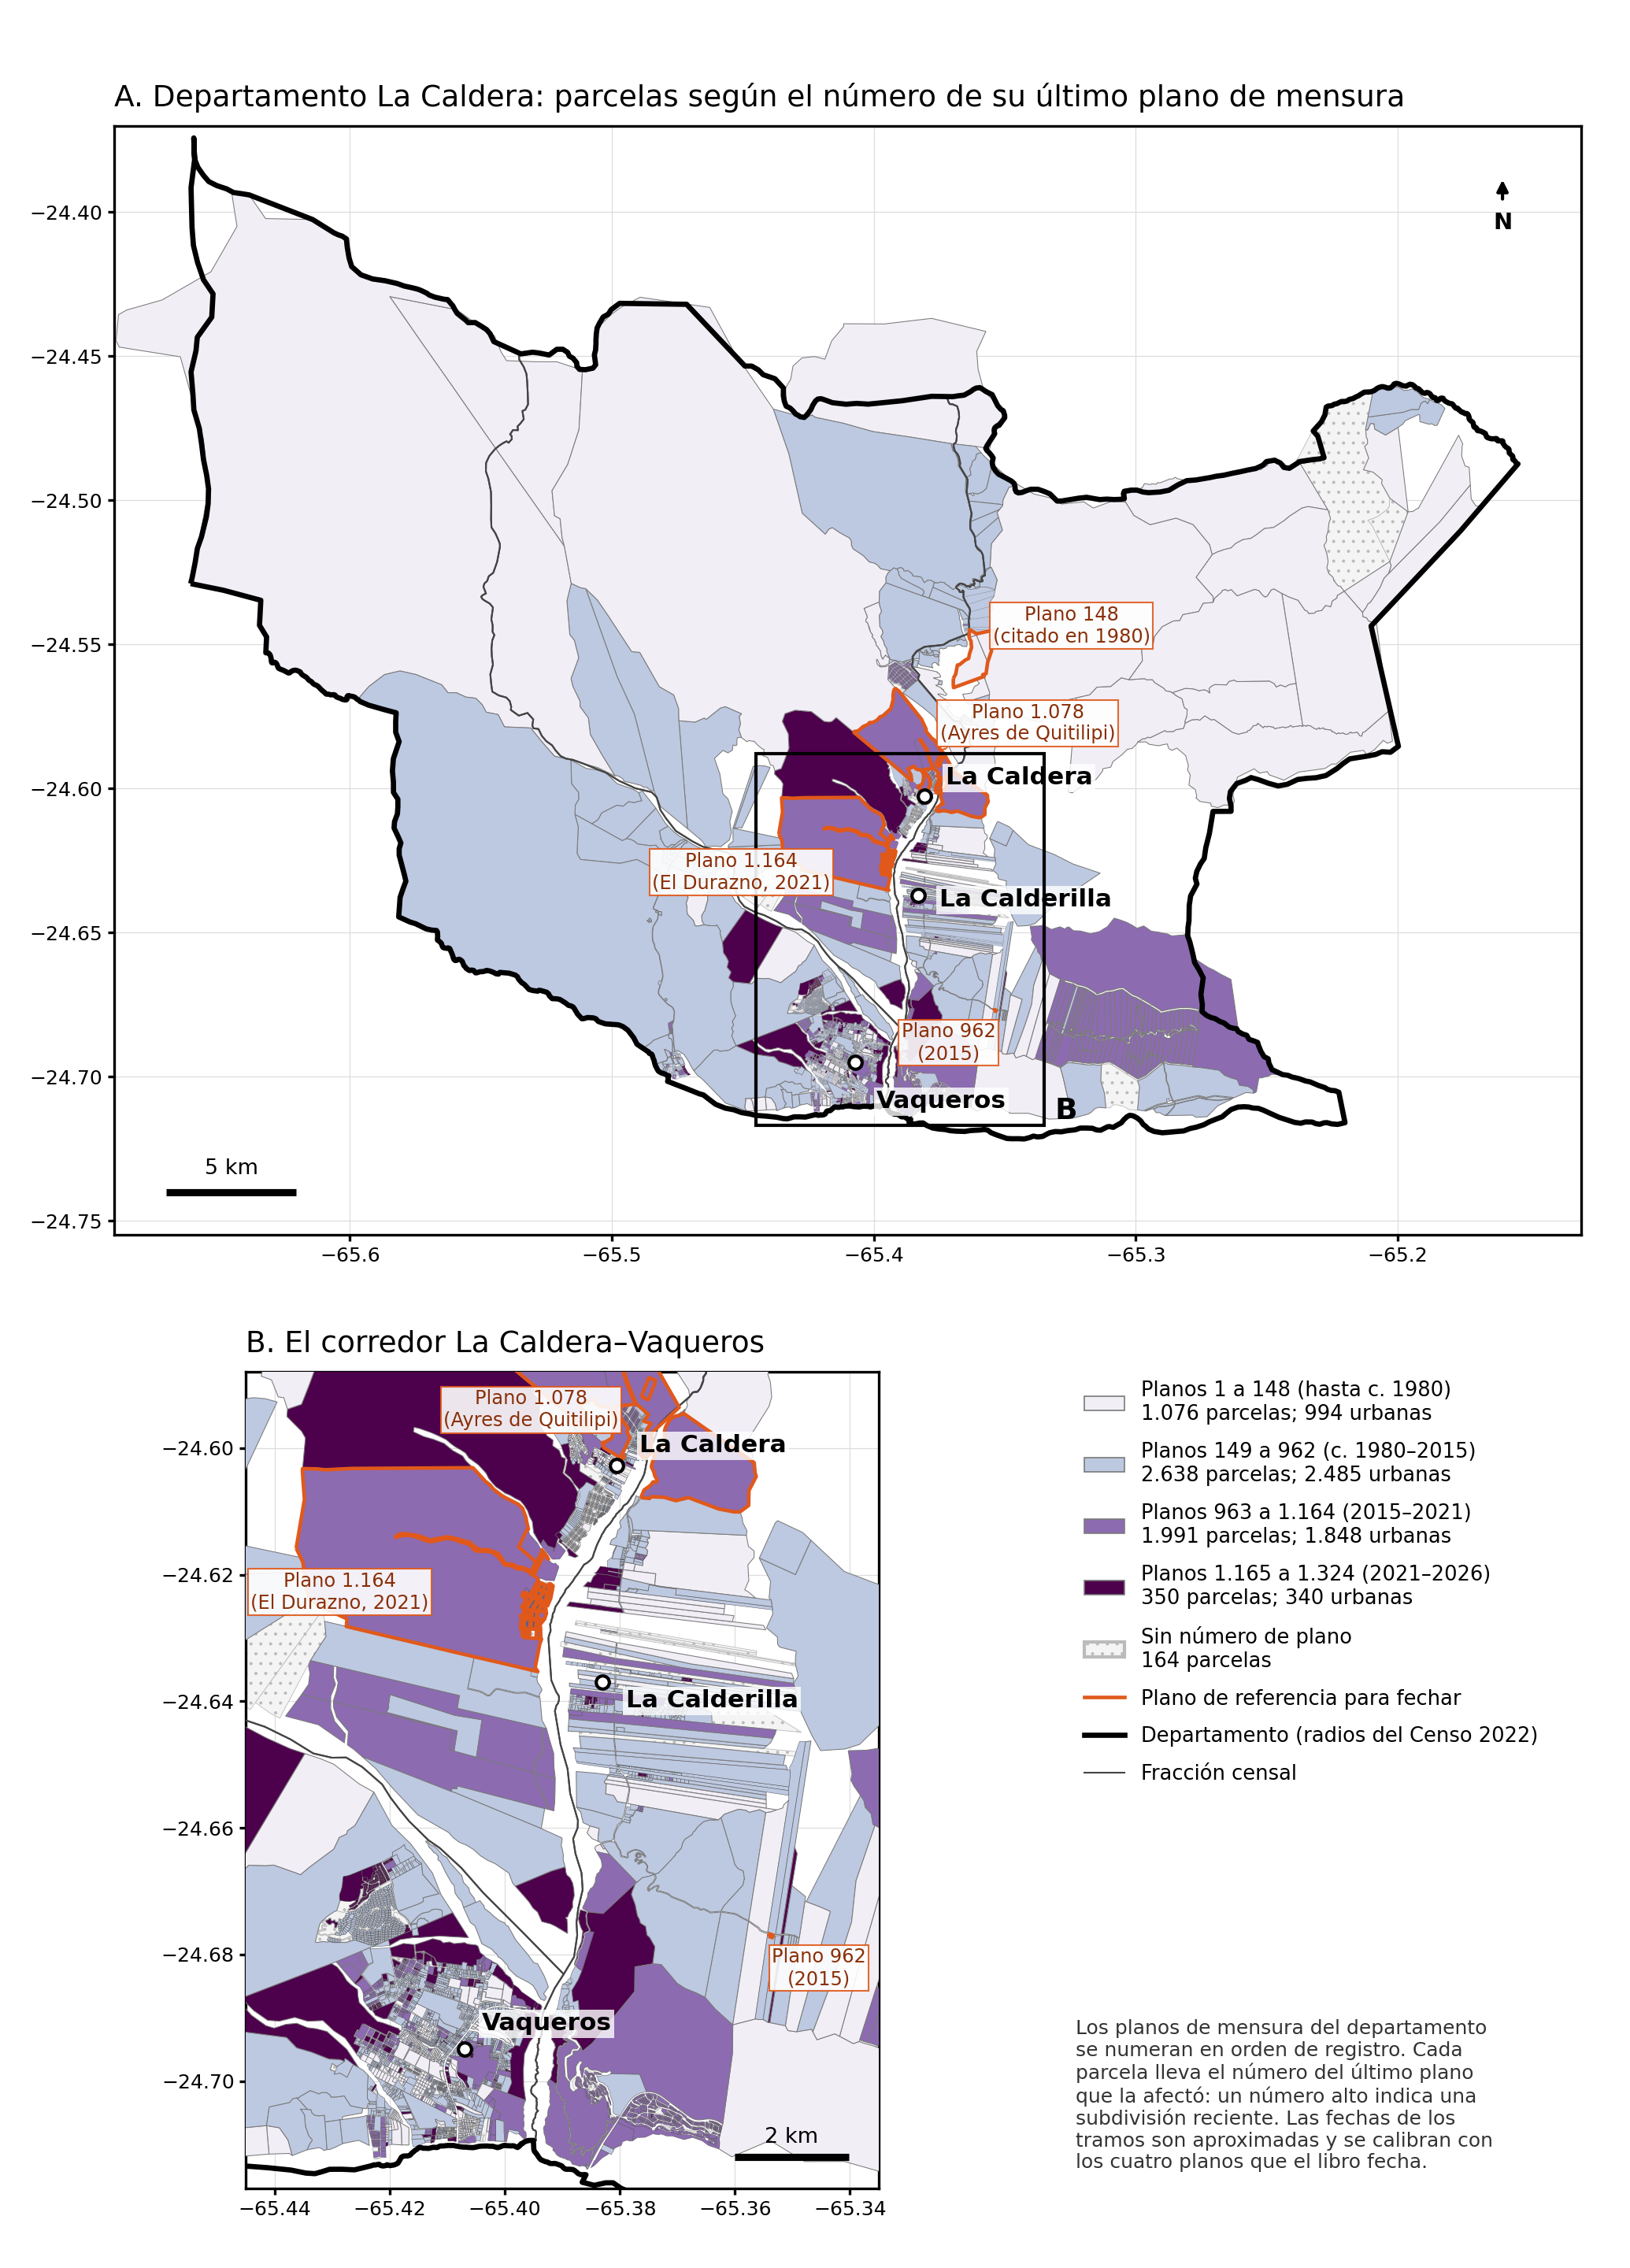
\includegraphics[width=\textwidth,height=0.84\textheight,keepaspectratio]{fig-planos-conversion.png}
\caption[La conversión, plano por plano]{\textbf{La conversión, plano por plano.} A: parcelas del departamento según el número del último plano de mensura que las afectó, agrupado en cuatro tramos; los tramos se fechan de modo aproximado con los cuatro planos que este libro documenta, recuadrados: el 148, citado por un decreto de 1980; el 962, de la prescripción de la escuela de Potrero de Gallinato (2015); el 1.078, que presentó Ayres de Quitilipi en 2020, y el 1.164 de El Durazno, aprobado en 2021. B: el corredor La Caldera--Vaqueros. Elaboración propia con el catastro parcelario de la Provincia (IDESA, consultado en septiembre de 2026) y la cartografía de radios del Censo 2022 (INDEC). Elaboración propia; dibujo de \texttt{scripts/mapa\_planos.py} del repositorio \texttt{mapas\_caldera} (apéndice \ref{cap:fuentes}).}\label{fig:planos}
\end{figure}

\section{La aprobación del plano, y lo que deja afuera}

El acto provincial que aprobó el loteo fue obtenido en su texto íntegro, y contiene el dato que ordena todo el capítulo.

\begin{ficha}{Resolución Nº 646 D del Ministerio de Infraestructura}
\begin{itemize}[leftmargin=*,nosep]
\item \textbf{Fecha:} 26 de noviembre de 2021. Boletín Oficial Nº 21.123 del 1 de diciembre. Expediente Nº \textbf{18-37.348/2019-0}. Firmante: Camacho.
\item \textbf{Objeto:} aprueba el Plano de Mensura, Desmembramiento y Loteo Nº 1.164 sobre la matrícula 6.558, \textbf{de propiedad de los Sres.\ Héctor D'Andrea\index{D'Andrea, Héctor} y Jardín Celestial S.R.L.}, correspondiente al proyecto ``El Durazno'' \textbf{en sus Etapas 1 y 2 (lámina 3/3) y Etapa 4 (lámina 2/3)}.
\item \textbf{Marco:} Título V de la Ley Nº 2.308 y su reglamentación por Decreto Nº 1.682/19.
\item \textbf{Intervenciones con foliatura:} Municipio de La Caldera, fs.\ 58, 84 y 97/101. \textbf{Secretaría de Recursos Hídricos, fs.\ 59.} Edesa S.A., fs.\ 62/67. Instituto Provincial de la Vivienda, fs.\ 60/61. Compañía Salteña de Agua y Saneamiento S.A., fs.\ 68. Dirección de Vialidad, fs.\ 106/108. Cartografía, Cálculo y Estudio de Títulos de la DGI, fs.\ 26/28 y 55; Asesoría Jurídica, fs.\ 124/125. Unidad Coordinadora de Loteos, fs.\ 137.
\item \textbf{Artículo 2º:} las matrículas individuales de cada lote se asignarán \textbf{una vez acreditada la aceptación de la donación} del espacio institucional y presentados los certificados de libre deuda del período fiscal 2021.
\end{itemize}
\end{ficha}

\subsection*{Las Etapas 3 y 5 no están}

La resolución aprueba las etapas 1, 2 y 4. \textbf{No aprueba la Etapa 3. Tampoco la 5.}

Y la sentencia del amparo consigna como afectados por los aluviones de diciembre de 2018 y enero de 2019 a los vecinos de los loteos \textbf{El Durazno I a V}. Es decir: \textbf{cinco etapas estaban vendidas y habitadas} cuando ocurrió el desastre.

Ordénense las fechas.

\textbf{Diciembre de 2018 y enero de 2019:} cinco etapas pobladas se inundan.

\textbf{2019:} se inician los expedientes 18-37.348 --- plano --- y 18-37.349 --- donación --- ante el Ministerio de Infraestructura. El mismo año de los aluviones, y el mismo año en que el Decreto 1682/19 reemplaza el régimen de 1973.

\textbf{Noviembre de 2021:} se aprueba el plano, sólo para las etapas 1, 2 y 4.

\textbf{Mayo de 2022:} se acepta la donación, condición para que se asignen las matrículas individuales.

\textbf{El loteo estuvo vendido y habitado al menos tres años antes de que la Provincia aprobara el plano de subdivisión.} Las familias que se inundaron en 2018 vivían en parcelas que aún no tenían matrícula propia, porque su asignación quedaba condicionada a un acto que ocurrió en 2022.

Y dos de las cinco etapas siguen, hasta donde alcanza este relevamiento, sin plano aprobado.

La capa catastral de Inmuebles descargada en 2026 muestra el resultado del plano 1164: \textbf{doscientas cuarenta y siete parcelas urbanas} (catastros 6714 a 6960), que suman veintisiete hectáreas con una mediana de 875 metros cuadrados, y \textbf{un remanente rural de 1.150 hectáreas} (catastro 6713). La matrícula 6558 ya no figura. Doscientos cuarenta y siete lotes con plano, contra los cuatrocientos para los que se gestionaba el agua en 2015: la diferencia es del orden de las etapas que siguen sin plano aprobado (capítulo \ref{cap:ribera}, apartado sobre la capa catastral).

\textbf{Y las dos magnitudes de este capítulo no cierran entre sí.} Si las doscientas cuarenta y siete parcelas suman veintisiete hectáreas ---sin contar calles, ochavas ni el espacio donado---, la superficie total del fraccionamiento excede las veintiséis y media que se deducen del 3,05 por ciento de la donación. Una de las dos cifras está mal: o el porcentaje del acto se calcula sobre otra base, o la medición de la capa no corresponde al mismo polígono. Lo resuelve el balance de superficies del plano 1.164. \pendiente{balance de superficies del plano de mensura, unificación, desmembramiento y loteo Nº 1.164}

\begin{ficha}{Cómo se tiene la vivienda propia --- Censo 2022}
Población en viviendas particulares propias, según la documentación de la propiedad. La Caldera: 9.187 personas; con escritura, 61,2\,\%; con \textbf{boleto de compraventa, 21,0\,\%}; con otra documentación, 9,8\,\%; sin documentación, 8,0\,\%. Provincia de Salta: con escritura, 55,3\,\%; con boleto, 10,2\,\%; con otra documentación, 14,1\,\%; sin documentación, 20,4\,\%. Departamento Capital: boleto, 6,6\,\%.

\textit{Fuente: INDEC, Censo 2022, resultados definitivos, cuadro 6.17 de condiciones habitacionales de la población, Salta; porcentajes de elaboración propia.}
\end{ficha}

\begin{cautela}
En La Caldera, uno de cada cinco habitantes de vivienda propia la tiene por boleto de compraventa: el doble del promedio provincial, más del triple que en la Capital, y la tercera proporción más alta de los veintitrés departamentos, detrás de Santa Victoria y La Candelaria. El boleto no es una irregularidad: es la forma normal de una compra cuya escritura todavía no se otorgó. Pero es exactamente la forma que adopta una compra de lote en un fraccionamiento cuyo plano no está aprobado y cuyas parcelas no tienen matrícula propia, que es lo que este capítulo documenta para El Durazno. El censo no dice qué parte de esas 1.928 personas vive en los loteos del corredor; dice que el departamento tiene una proporción de propietarios con boleto de compraventa que duplica la provincial ---la de propietarios sin escritura por cualquier causa es, en cambio, menor que la provincial---, en un territorio donde la informalidad sin papeles ---el 8 por ciento--- es menos de la mitad de la provincial. La falta de escritura, aquí, no es la del asentamiento precario: es la de la compra formal a medio terminar.
\end{cautela}

\begin{cautela}
\textbf{Una discrepancia que este libro no resuelve.} El registro de loteos que la Municipalidad elevó a Fiscalía de Estado en septiembre de 2022 (capítulo \ref{cap:amparo}) no coincide con la Resolución 646D/21: consigna como aprobadas las etapas I, III y IV, y como irregulares la II y la V. La resolución provincial aprobó la 1, la 2 y la 4. Puede tratarse de numeraciones distintas, de una aprobación posterior o de un error en una de las dos fuentes. Lo que no cambia es que en 2022 al menos dos etapas carecían de aprobación, y que la quinta figura sin ella en ambas.
\end{cautela}

\begin{cautela}
La foja 59 concentra la pregunta más productiva de todo el expediente.

Es la intervención de la \textbf{Secretaría de Recursos Hídricos} en el trámite de aprobación del plano. Ese es el mismo organismo que había aprobado, por Resolución 383 del 18 de diciembre de 2014, la determinación de la línea de ribera de ambas márgenes de los arroyos El Durazno y Guaranguay; y el mismo que, citado en el amparo, pidió el rechazo de la demanda sosteniendo que no tenía capacidad para hacer obras.

Qué dijo esa Secretaría, entre 2019 y 2021, sobre un loteo emplazado en la microcuenca que se había desbordado y cuya línea de ribera ella misma había fijado cinco años antes, es un documento de una sola foja que este libro no consultó.
\end{cautela}

\section{El texto de la Resolución 646D/21}

Se obtuvo la resolución completa, publicada en el Boletín Oficial Nº 21.123 del 1 de diciembre de 2021. Dictada el 26 de noviembre de 2021 por el Ministro de Infraestructura, en el expediente 18-37.348/2019-0, con firma de Camacho.

\begin{ficha}{Mapa de fojas del expediente 18-37.348/2019-0}
La resolución acredita, foja por foja, quién intervino:
\begin{itemize}[leftmargin=*,nosep]
\item \textbf{Municipio de La Caldera:} fs.\ 58, 84 y 97/101.
\item \textbf{Secretaría de Recursos Hídricos:} fs.\ 59.
\item \textbf{Instituto Provincial de la Vivienda:} fs.\ 60/61.
\item \textbf{Edesa S.A.:} fs.\ 62/67.
\item \textbf{Compañía Salteña de Agua y Saneamiento S.A.:} fs.\ 68.
\item \textbf{Dirección de Vialidad de Salta:} fs.\ 106/108.
\item Cartografía, Cálculo y Estudio de Títulos de la D.G.I.: fs.\ 26/28 y 55.
\item Asesoría Jurídica de la D.G.I.: fs.\ 124/125.
\item \textbf{Unidad Coordinadora de Loteos, Loteadores y Desarrolladores} (art.\ 11 del Decreto 1682/19): fs.\ 137.
\item Coordinación Legal y Técnica del Ministerio: fs.\ 128/129 y 140.
\end{itemize}
Competencia invocada: art.\ 27 de la Ley 8.171, modificada por la Ley 8.274, y Decreto 1682/19.
\end{ficha}

Dos precisiones que el texto permite y que antes eran conjetura.

\textbf{Primera: la lámina que falta.} El artículo 1 aprueba el plano 1.164 respecto de las Etapas 1 y 2 --- lámina 3/3 --- y de la Etapa 4 --- lámina 2/3. La numeración indica que el plano tiene \textbf{tres láminas}. La lámina 1/3 no se menciona en ninguna parte de la resolución. Qué contiene, y si corresponde a las etapas no aprobadas, es una pregunta de una sola foja.

\textbf{Segunda: qué condiciona la matrícula.} El artículo 2 dispone que la Dirección General de Inmuebles asignará las matrículas individuales \textbf{una vez acreditadas dos cosas}: la aceptación por la Provincia de la donación del espacio de uso institucional, y los certificados de libre deuda del período fiscal 2021.

No figura, entre las condiciones, la ejecución de obra alguna. Un apartado posterior de este capítulo muestra que el régimen anterior --- el Decreto 1.410/73, cuyo texto también se obtuvo --- condicionaba la asignación de matrícula al cumplimiento previo de las obras y servicios comprometidos, verificado por la Municipalidad. La comparación entre ambos artículos es el hallazgo que ese apartado desarrolla.

Y una lectura que corresponde hacer con cuidado, porque es fácil forzarla.

La resolución dice que los organismos de contralor intervinieron para ``garantizar que la urbanización propuesta verifique el acceso a infraestructura y servicios básicos'', y enumera seis, entre ellos Recursos Hídricos y la empresa de agua y saneamiento. La resolución no dice qué dictaminó cada uno. Un expediente puede registrar la intervención de un organismo que se expidió en contra, o con condiciones, o que se limitó a tomar conocimiento.

Por eso la foja 59 --- una sola foja de Recursos Hídricos --- sigue siendo la pregunta más productiva del expediente, y ahora se sabe exactamente dónde está. Junto a ella, la foja 68 de la empresa de agua y las fojas 58, 84 y 97/101 del Municipio, que es donde debería constar qué dijo el municipio cuyos representantes declararon después que una etapa carecía de autorización.

Una aclaración de nomenclatura, para que quien continúe este trabajo no pierda tiempo. Existe una \textbf{Resolución 383/14 de la Secretaría de Obras Públicas} del Ministerio de Economía, que aprueba el legajo técnico de un centro sanitario en el departamento Orán y se publicó en el Boletín Nº 19.346 del 21 de julio de 2014. \textbf{No tiene relación con este capítulo.} La Resolución 383 que aquí importa es de la \textbf{Secretaría de Recursos Hídricos}, del 18 de diciembre de 2014, y se conoce por el edicto publicado en el Boletín Nº 19.467 en enero de 2015. Cada organismo lleva su propia serie de numeración anual, de modo que el mismo número y el mismo año corresponden a actos distintos. Al pedirla hay que identificar el organismo, no sólo el número. Lo mismo vale para la Resolución 185/14: la Secretaría de Ambiente dictó una con ese número sobre la recepción de acumuladores eléctricos usados, publicada en el Boletín Nº 19.281 del 10 de abril de 2014, que tampoco tiene relación con la línea de ribera de la matrícula 4366 que la Secretaría de Recursos Hídricos aprobó bajo el mismo número en julio.

\subsection*{Diez días antes de la audiencia}

El 2 de febrero de 2026, el municipio de La Caldera publicó en su sitio oficial un parte sobre las tareas en curso tras el temporal de enero.

\begin{ficha}{Parte municipal, 2 de febrero de 2026 --- área Obras Públicas}
``Gracias a las gestiones realizadas por el municipio, se dispuso de \textbf{maquinaria pesada} contratada y aportada por organismos provinciales. Con estos equipos ya se ejecutaron ---y continúan desarrollándose--- tareas de \textbf{construcción de bateas} en distintos tramos del río La Caldera, además de trabajos de \textbf{encauzamiento} y la \textbf{construcción de muros de contención}.''

Se agrega que esas acciones ``se suman a las obras de encauzamiento y bateas realizadas en la zona sur de la localidad'', y que el objetivo es mejorar el escurrimiento y evitar desbordes ante nuevas lluvias.
\end{ficha}

\begin{cautela}
La fecha importa. Diez días después, el 12 de febrero, la jueza aprobó el Plan de Manejo Integral y ratificó el marco de la condena de 2021, que exigía una estrategia basada en infraestructura verde --- reforestación, relocalización de elementos obstructores --- \textbf{por sobre} la infraestructura gris, definida en la propia sentencia como obras civiles, maquinaria pesada y edificación hormigonada.

Bateas, encauzamiento, muros de contención y maquinaria pesada son, término por término, el catálogo que la sentencia subordinó. Y en noviembre de 2025, según la cobertura de prensa ---la lista de actuaciones del expediente que el capítulo \ref{cap:amparo} reconstruye no registra ese acto---, se habría ordenado a provincia y municipio reparar el daño causado por la extracción irregular de áridos, que es la actividad que altera los canales subálveos por la misma vía.

\textbf{Este libro no sostiene que esas obras incumplan la sentencia}, y hay razones serias para no afirmarlo. La condena estableció una prelación, no una prohibición: no dijo que no se hicieran obras civiles, dijo que no fueran la estrategia principal. Un temporal reciente puede justificar intervención inmediata sobre el escurrimiento, y el propio Plan aprobado puede contemplarlas. Este libro leyó el Plan, pero no pudo establecer si estas tareas concretas están comprendidas en sus medidas ni si se comunicaron al tribunal.

Lo que queda registrado es que la respuesta municipal al temporal de enero de 2026, tal como el municipio la comunica, se describe íntegramente en el vocabulario de la infraestructura gris, sin una sola mención a reforestación, a relocalización de obstructores ni a la restauración de márgenes. Y que se ejecutó mientras el expediente estaba en trámite. Contrastar ese parte con el texto del Plan es, otra vez, la comprobación que este capítulo viene señalando.
\end{cautela}

\section{Cuatrocientos lotes con agua, seis años antes del plano}

En julio de 2015 la Secretaría de Recursos Hídricos publicó, cinco días seguidos, una gestión que este libro no conocía y que reordena la cronología entera del loteo.

\begin{ficha}{Concesión de agua pública --- B.O.\ Nº 19.577 a 19.581, 10 al 16 de julio de 2015}
Expediente 0090034-211560/2014-0.

``\textbf{Magdalena Vidal\index{Vidal, Magdalena}}, \textbf{co-titular registral del inmueble Catastro Nº 4366} del Dpto.\ La Caldera, gestiona \textbf{la finalización del trámite} de concesión de agua pública subterránea de \textbf{dren horizontal}, sito en margen derecha del Río La Caldera, para \textbf{abastecimiento poblacional de 400 Lotes del Loteo `El Durazno'}, con un volumen total anual de \textbf{0,28908 hm³} comprensivos de 33 m³/hora con 24 horas de bombeo diarios, \textbf{con carácter permanente}, y para riego de espacios comunes de 3 hectáreas con una dotación de 1,575 l/s, con carácter eventual.''

Firma: Dra.\ Silvia F.\ Santamaría\index{Santamaría, Silvia F.}, Jefe del Programa Fiscalización y Control. Secretario de Recursos Hídricos: Ing.\ Alfredo Fuertes.
\end{ficha}

\begin{cautela}
Cinco cosas, y cada una toca un punto distinto del libro.

\textbf{Primera: el loteo tenía cuatrocientos lotes en 2015.} El plano de El Durazno se aprobó por Resolución 646D en \textbf{noviembre de 2021}, y sólo respecto de las etapas 1, 2 y 4. Seis años antes, el Estado provincial tramitaba el agua para \textbf{cuatrocientos lotes} de ese mismo loteo, y lo hacía bajo el rótulo de \textbf{``abastecimiento poblacional''} --- es decir, para gente que vive.

\textbf{Segunda: aparece una co-titular registral.} \textbf{Magdalena Vidal\index{Vidal, Magdalena}}, se presenta como co-titular del catastro 4366. Este libro conocía a Héctor D'Andrea\index{D'Andrea, Héctor} y a Jardín Celestial S.R.L.\ como copropietarios de la matrícula 6.558, sobre la que se aprobó el plano. La 4366 es la Finca La Caldera o Getsemaní, sobre la que recaen las líneas de ribera de sus cuatro cursos. Quiénes son sus co-titulares, en qué proporción y desde cuándo es exactamente el antecedente dominial que este libro viene pidiendo, y ahora tiene un nombre por donde empezar.

\textbf{Tercera: el organismo sabía.} La misma Secretaría que en diciembre de 2014 determinó la línea de ribera de los arroyos El Durazno y Guaranguay sobre el catastro 4366 --- sin publicar sus coordenadas --- tramitaba siete meses después, sobre el mismo catastro, el agua para cuatrocientos lotes del loteo llamado El Durazno. No son dos expedientes que se ignoran: es el mismo organismo, el mismo inmueble y el mismo nombre.

\textbf{Cuarta: la dotación.} Los 0,28908 hectómetros cúbicos anuales equivalen a 289.080 metros cúbicos, o 792 por día. Repartidos entre cuatrocientos lotes son \textbf{casi dos metros cúbicos diarios por lote}. Compárese con la concesión del Catastro 1700, de junio de 2014: veinticuatro metros cúbicos diarios para ciento veinte personas, es decir doscientos litros por persona. La de El Durazno es varias veces más generosa por unidad.

\textbf{Y quinta, que es la que exige más cuidado.} El aviso dice ``concesión de agua pública \textbf{subterránea}'' y, en el mismo párrafo, ``\textbf{con carácter permanente}''. El artículo 143 del Código de Aguas establece que ``las concesiones de uso de aguas subterráneas, salvo las que se hubieran obtenido por declaración judicial de aguas privadas, \textbf{serán eventuales}''.

Este libro \textbf{no afirma} que haya aquí una irregularidad. Un dren horizontal en la margen de un río capta agua del subálveo, y es posible que el régimen la asimile al curso superficial y no al acuífero profundo, en cuyo caso el carácter permanente sería correcto y el artículo 143 no se aplicaría. Es una cuestión técnico-jurídica que excede a este trabajo.

Lo que en efecto corresponde registrar, y es verificable, es el \textbf{contraste}: en el mismo departamento, ante el mismo organismo y con trece meses de diferencia, un abastecimiento poblacional de agua subterránea para ciento veinte personas se otorgó como \textbf{eventual}, y otro para cuatrocientos lotes se tramitó como \textbf{permanente}.
\end{cautela}

\begin{cautela}
Y la reserva que este libro se impuso --- que un dren horizontal podría asimilarse al curso superficial y quedar fuera del artículo 143 --- \textbf{no alcanza al tercer caso}.

En octubre de 2015, El Chalchal S.R.L., cotitular del \textbf{catastro 3616}, gestionó para el Loteo ``La Misión Etapa III'' la finalización de una concesión de \textbf{agua pública subterránea de pozo perforado}, para 580 habitantes en 116 lotes, ``con \textbf{carácter permanente}'': nueve metros cúbicos por hora durante veintidós horas diarias, unos 340 litros por habitante por día. El catastro 3616 es el mismo sobre el que la Resolución 142/14 había determinado, sin publicar coordenadas, la línea de ribera de los ríos Mojotoro y La Caldera (capítulo \ref{cap:ribera}). (Diez años después, en 2025, la misma firma vuelve a figurar en el Boletín como cotitular de otro inmueble del departamento, el catastro 5925, gestionando agua del arroyo Los Mártires para cien cabezas de ganado; capítulo \ref{cap:aguabaja}.) Un pozo perforado no admite discusión sobre su naturaleza: es agua subterránea en el sentido literal del artículo 143, que declara eventuales todas esas concesiones salvo las de aguas privadas declaradas judicialmente.

De modo que el cuadro queda así, y es puramente descriptivo:

\begin{center}\small
\begin{tabular}{@{}p{3.7cm}p{2.5cm}p{2.4cm}p{2.9cm}@{}}
\toprule
\textbf{Destinatario} & \textbf{Fuente} & \textbf{Fecha} & \textbf{Carácter} \\
\midrule
120 habitantes, catastro 1700 & Pozo perforado & jun.\ 2014 & \textbf{Eventual} \\
400 lotes, loteo El Durazno & Dren horizontal & jul.\ 2015 & \textbf{Permanente} \\
580 habitantes, loteo La Misión III & \textbf{Pozo perforado} & oct.\ 2015 & \textbf{Permanente} \\
\bottomrule
\end{tabular}
\end{center}

Tres gestiones de abastecimiento poblacional, ante el mismo organismo, firmadas por la misma funcionaria, en dieciséis meses. Dos de las tres son de pozo perforado y recibieron tratamientos opuestos.

\textbf{Este libro sigue sin afirmar que exista irregularidad}, y sostiene la reserva por una razón concreta: no encontró en el Código de Aguas ni en su reglamentación ---que obtuvo completos--- una norma que distinga estas situaciones, y no conoce las resoluciones finales de ninguno de los tres trámites --- los avisos publican \textbf{gestiones}, no otorgamientos. Es enteramente posible que la ley admita el carácter permanente en supuestos que estas líneas no identifican.

Lo que registra es que la diferencia existe, es verificable en el Boletín Oficial y \textbf{correlaciona con el tamaño del solicitante}: la concesión eventual es la de ciento veinte personas; las permanentes, las de cuatrocientos y quinientos ochenta. Preguntarlo es legítimo y la respuesta está en tres expedientes identificados por número.
\end{cautela}

\textbf{Un cuarto caso, del mismo año de inicio.} El expediente 0090034-88064/2015 ---iniciado en 2015, como el de La Misión III--- llega al Boletín en abril de 2019: \textbf{Valle Hermoso S.R.L.}\ «gestiona la finalización del trámite de concesión de agua pública subsuperficial (de dren horizontal) para abastecimiento poblacional del loteo Valle Hermoso», en el catastro 3.307, por 15,71 metros cúbicos por hora con dieciséis horas diarias de bombeo ---0,092 hectómetros cúbicos al año---, \textbf{con carácter permanente}. Firma la misma funcionaria, y la publicación se repite cinco veces, entre el 26 de abril y el 3 de mayo de 2019. Es otro loteo que pide agua de un dren subsuperficial, con el mismo carácter que el de El Durazno; el aviso no dice de qué curso.

Y hay una consecuencia cronológica que el capítulo debe enunciar sin adornos.

El primer aluvión ocurrió el 21 de diciembre de 2018. Para entonces, según esta gestión, el loteo El Durazno llevaba al menos tres años y medio con trámite de agua en curso para cuatrocientos lotes destinados a abastecimiento poblacional. El plano se aprobaría tres años después del aluvión.

Este libro ya había documentado que los lotes se vendieron y se habitaron antes de la aprobación. Lo nuevo es que \textbf{el Estado provincial estaba dotando de agua a esa población} mientras el fraccionamiento carecía de plano aprobado, y que el organismo que lo hacía era el mismo que había fijado la línea de ribera de los arroyos que iban a desbordarse.

\section{Quién es Jardín Celestial S.R.L.}

La sociedad aparece en este libro por tres vías documentales independientes: es copropietaria del inmueble sobre el que se aprobó el plano, figura como tercero en el expediente judicial, y su composición consta en avisos publicados en el Boletín Oficial.

\begin{ficha}{Constitución --- Boletín Oficial Nº 18.481, 1 de diciembre de 2010}
Instrumento del 13 de octubre de 2010. Publicación autorizada por el Juez de Minas y en lo Comercial de Registro. Domicilio social: Sarmiento 122, ciudad de Salta. Duración: 50 años. Capital: \$180.000 en 1.800 cuotas.

\textbf{Objeto social:} instalación, construcción y administración del funcionamiento de un \textbf{Cementerio Parque} y todo lo inherente a su explotación \textbf{en la jurisdicción del departamento La Caldera}.

\textbf{Socios:} Héctor D'Andrea\index{D'Andrea, Héctor}, 44 años, empresario, domiciliado en Finca Getsemaní, La Caldera --- 990 cuotas, 55\%; Carlos Miguel Calabró\index{Calabró, Carlos Miguel}, 19 años, estudiante, domiciliado en Los Crisantemos s/n, La Caldera --- 540 cuotas, 30\%; y Renzo Daniel Palacios, 48 años, empresario, domiciliado en la provincia de San Juan --- 270 cuotas, 15\%. Socio gerente: Palacios. Suplente: D'Andrea.
\end{ficha}

\begin{ficha}{Modificación --- Boletín Oficial Nº 19.394, 29 de septiembre de 2014}
Acta de reunión de socios del 26 de mayo de 2014. Se modifica el objeto: la sociedad ``también podrá dedicarse a la \textbf{comercialización de inmueble de terceros}, y cuando las finanzas lo permitan podrán \textbf{adquirir inmueble para su futura realización, para este último caso se requerirá un acta que contenga el acuerdo entre los socios para cada inmueble} en oportunidad que se llegará a la adquisición''. El objeto conserva además la facultad de ``construir edificios, obras de infraestructura y todas las obras necesarias''.

Se capitalizan aportes irrevocables efectuados en agosto de 2012 \textbf{para la compra de un camión Ford, dominio JT0712}, y el capital se eleva a \$545.000 en 5.450 cuotas. Participaciones resultantes: D'Andrea\index{D'Andrea, Héctor} 2.453 cuotas (45,01\%), Calabró 1.635 (30,00\%), Palacios 1.362 (24,99\%). Certifica la Dra.\ María Luján Genovese, secretaria interina del Juzgado de Minas y en lo Comercial de Registro.
\end{ficha}

Tres detalles del texto completo que conviene retener.

\textbf{El primero:} la adquisición de inmuebles quedó sujeta a \textbf{un acta de acuerdo entre los socios para cada inmueble}. No es una cláusula de estilo. Significa que cada compra de tierra por parte de la sociedad debía dejar constancia societaria propia, y que esas actas existen. Son el documento que registraría, socio por socio y fecha por fecha, cómo la firma pasó de administrar un cementerio a ser copropietaria del inmueble de un loteo.

\textbf{El segundo, que la ficha muestra y conviene leer:} el aumento de capital \textbf{reordenó las participaciones}. D'Andrea baja del 55 al 45,01 por ciento y pierde la mayoría absoluta; Palacios sube del 15 al 24,99; y Calabró queda en \textbf{30,00 por ciento exacto}, la única cifra redonda de las tres. Ocurre en el mismo acto en que el objeto social se amplía a la compra y comercialización de inmuebles. Este libro no sabe qué lo explica ---la capitalización de aportes desiguales lo produce sin necesidad de acuerdo alguno--- y lo registra porque es el único movimiento societario documentado de la firma entre su constitución y la aprobación del plano.

\textbf{El tercero:} el aumento de capital de 2014 capitaliza aportes hechos en \textbf{agosto de 2012 para comprar un camión}. Una sociedad cuyo objeto declarado era un cementerio parque capitalizó, dos años después, la compra de un vehículo de carga. Puede ser enteramente funcional a la construcción del cementerio. Se consigna porque fecha una inversión en 2012, en el período que este libro tiene menos documentado.

\begin{ficha}{Renovación del órgano de administración --- Boletín Oficial Nº 20.675, 30 de enero de 2020}
Acta de reunión ordinaria del \textbf{8 de noviembre de 2018}. Gerente Titular: Héctor D'Andrea\index{D'Andrea, Héctor}. \textbf{Gerente Suplente: Héctor Miguel Calabró\index{Calabró, Héctor Miguel}}, con el mismo número de documento que consta para él en el acta de proclamación de 2011 (capítulo \ref{cap:politica}), quien acepta el cargo y constituye domicilio especial en Sarmiento 122.
\end{ficha}

Héctor Miguel Calabró\index{Calabró, Héctor Miguel} fue \textbf{intendente de La Caldera} --- accedió en 1999 y fue reelecto en 2003 y 2007 ---, \textbf{diputado provincial} por el departamento entre 2011 y 2015, secretario de Relaciones Institucionales del Ministerio de Gobierno desde diciembre de 2015 (Decreto 89/15, B.O.\ Nº 19.684 del 17/12/2015) y \textbf{Secretario de Asuntos Municipales} de la Provincia desde noviembre de 2017 (Decreto 1634/17, B.O.\ Nº 20.155 del 30/11/2017, dictado junto con el Decreto 1608/17, que aceptó desde el 23 de noviembre de 2017 su renuncia al cargo anterior) hasta el final de la gestión Urtubey, en 2019 ---en 2018 una decisión administrativa le asignó el adicional por responsabilidad del cargo; la fecha del cese proviene de la prensa---; los dos decretos lo identifican con el mismo número de documento que el acta de proclamación de 2011 y el aviso societario de 2020, y \textbf{senador provincial} por La Caldera entre diciembre de 2021 y diciembre de 2025.

La secuencia documentada, entonces, es la siguiente:

\begin{itemize}[leftmargin=1cm,itemsep=2pt]
\item La sociedad se constituye en octubre de 2010, \textbf{durante su tercera intendencia}, con un socio de diecinueve años que comparte su apellido y su segundo nombre, suscriptor del 30\% del capital y con objeto social expresamente circunscripto \textbf{a la jurisdicción que gobierna}.
\item El objeto se amplía a la comercialización y adquisición de inmuebles en mayo de 2014, \textbf{mientras es diputado provincial por ese departamento}.
\item Él mismo ingresa al órgano de administración en noviembre de 2018, \textbf{mientras es Secretario de Asuntos Municipales de la Provincia}.
\item El plano del loteo se aprueba en noviembre de 2021, \textbf{cuando es senador provincial electo por ese departamento}, a días de asumir la banca.
\end{itemize}

\begin{cautela}
Corresponde establecer con precisión qué prueba y qué no prueba esta secuencia, porque es el punto del libro donde más fácil sería excederse.

\textbf{No prueba ilicitud.} Participar en una sociedad comercial no lo es. Que un pariente de un funcionario sea socio de una firma, tampoco. Que un funcionario provincial ---en noviembre de 2018 era Secretario de Asuntos Municipales--- acepte un cargo de gerente suplente en una empresa privada, tampoco, aunque sí plantea la pregunta por el régimen de incompatibilidades que le correspondía. Y el gerente suplente de una sociedad de responsabilidad limitada no administra: reemplaza al titular en caso de ausencia o vacancia.

\textbf{No prueba que el loteo se haya aprobado por influencia.} La aprobación provincial del plano tramitó entre 2019 y 2021, período en el cual la intendencia de La Caldera \textbf{no era ejercida por Calabró} sino por Diego Sumbay\index{Sumbay, Diego Ramiro}, en funciones desde 2019. La intervención municipal que consta en el expediente corresponde a esa gestión.

\textbf{Y hay un registro que apunta en dirección contraria y que este libro documenta.} En diciembre de 2024, siendo senador, Calabró fue uno de \textbf{sólo tres votos negativos} a la Ley provincial 8483 de revisión del Ordenamiento Territorial de Bosques Nativos. Impulsó además la prórroga de la ley de suspensión de desalojos de familias rurales. Ambos actos son restrictivos respecto del avance sobre bosque nativo y protectores respecto de la tenencia precaria.

\textbf{Lo que en cambio establece la secuencia} es una convergencia sostenida durante quince años entre el ejercicio de función pública sobre un territorio y la participación societaria en una firma que opera suelo en ese mismo territorio. Y establece que la sociedad titular del loteo que se inundó, y que es parte del expediente judicial que litiga por esa inundación, tuvo entre sus socios a alguien que comparte apellido y segundo nombre con el intendente bajo cuya gestión se constituyó.

Nada de eso equivale a una imputación, y este libro no la formula.
\end{cautela}

\begin{cautela}
Dos advertencias de método, que valen para este apartado más que para ningún otro del libro.

\textbf{Primera.} Carlos Miguel Calabró\index{Calabró, Carlos Miguel} no ejerció función pública electiva. Es una persona privada que figura en avisos comerciales publicados en el Boletín Oficial. Se lo nombra porque esos avisos son públicos y porque la sociedad de la que fue socio es el objeto central de este capítulo, no por su vínculo familiar. Toda referencia a él se limita a lo que consta en esos instrumentos.

\textbf{Segunda.} Esta línea de investigación llegó a este trabajo por un encargo formulado por un tercero interesado, con nombre puesto de antemano. Se la siguió aplicando los mismos estándares que al resto del libro: instrumentos públicos, cotejo de documentos de identidad, y consignación expresa de lo que apunta en sentido contrario. Antes de cualquier publicación corresponde ofrecer a las personas y a la sociedad nombradas la posibilidad de responder por escrito.
\end{cautela}

\section{El circuito}

El proceso por el cual una hectárea de monte de yungas se convierte en parcelas vendibles atraviesa, en el departamento La Caldera, una secuencia relativamente estable.

\begin{enumerate}
\item \textbf{Titularidad.} Parcela madre de gran superficie, de origen sucesorio o institucional.
\item \textbf{Estructuración jurídica.} Fideicomiso, sociedad o convenio con un desarrollador. Es el paso donde el titular original se desprende del riesgo sin desprenderse del beneficio.
\item \textbf{Apertura física.} Movimiento de suelo, apertura de caminos, demarcación de lotes.
\item \textbf{Habilitación ambiental.} Expediente ante la Secretaría de Ambiente provincial, dictamen técnico y audiencia pública cuando corresponde, conforme la ley 7070.
\item \textbf{Habilitación municipal.} Certificado de aptitud ambiental municipal, ordenanza del Concejo, aprobación de plano de mensura.
\item \textbf{Comercialización.} Preventa, escrituración.
\item \textbf{Provisión de servicios.} Agua, cloacas, energía, defensas hidráulicas y caminos.
\end{enumerate}

El punto de falla no es ninguno de los pasos individualmente sino el orden en que efectivamente ocurren. Los casos relevados muestran apertura física antes de habilitación --- La Falda ---, comercialización antes de provisión de servicios --- El Durazno, Solanas ---, y aprobación municipal tramitando en paralelo a sanciones ambientales provinciales todavía vigentes --- el caso denunciado por el centro vecinal de La Calderilla.

Un procedimiento cuyos pasos son correctos pero cuya secuencia es reversible no es un procedimiento: es una formalidad posterior al hecho consumado. Y el paso séptimo queda, sistemáticamente, sin resolver o trasladado al Estado.

\section{Solanas de La Caldera}

El 21 de enero de 2026 el Concejo Deliberante celebró su Sesión Extraordinaria Nº 01, convocada por el Ejecutivo para tratar cuestiones urgentes vinculadas a ordenanzas vigentes y a la situación generada por las lluvias.

\begin{ficha}{Sesión Extraordinaria Nº 01/2026}
Según cobertura de \textit{Nuevo Diario de Salta} del 23/01/2026:
\begin{itemize}[leftmargin=*,nosep]
\item \textbf{Res. 01/26:} prórroga de la Ordenanza Nº 733.
\item \textbf{Res. 02/26:} solicitud de clausura preventiva del ingreso al Loteo Cerrado \textbf{Solanas de La Caldera}.
\item \textbf{Res. 03/26:} solicitud de clausura de los campings ``Los Teros'' y ``Papi Lalo''.
\item \textbf{Res. 04/26:} pedido de partidas para obras de defensa en el barrio Santiago Apóstol y en la zona sur.
\end{itemize}
Se promulgaron además las Ordenanzas Nº 830, 831 y 832.
\end{ficha}

El pedido de clausura se funda en un hecho del 4 de enero de 2026: el ingreso al loteo cedió y provocó daños en media calzada de la Ruta Nacional 9, a la altura del kilómetro 1618, con riesgo para la seguridad vial. El medio consigna que el loteo es copropiedad de Silvina Abilés.

El emprendimiento es ofrecido al público por la inmobiliaria Cabrera Bienes Raíces, con domicilio en calle Zuviría 642 de la ciudad de Salta, que le dedica una página propia en su sitio institucional. El material gráfico fue publicado en diciembre de 2024, lo que sitúa la comercialización activa al menos desde esa fecha. La página no consigna cantidad de lotes, superficies, precios, desarrollador ni obras comprometidas: se compone íntegramente de imágenes.

La fecha es el dato que sirve. Si la comercialización estaba activa en diciembre de 2024, los artículos 144 y 145 del Código --- garantía de ejecución de obras previa y licencia municipal de comercialización --- regían plenamente sobre este emprendimiento. El pedido de acceso a la información sobre esos dos actos debe formularse en primer término respecto de Solanas, porque es el caso donde la fecha de comercialización está documentada y el hecho posterior --- el desprendimiento del ingreso sobre una ruta nacional --- también.

Que la página comercial no informe superficie, cantidad de parcelas ni obras comprometidas es además relevante bajo el artículo 149 del mismo Código, que regula acceso a la información y defensa del consumidor en urbanizaciones.

Sobre la copropiedad, el libro fija su posición aquí y la sostiene hasta el final.

El capítulo \ref{cap:tierrafiscal} documenta, con el Decreto Nº 64/23, que María Silvina Abilés fue designada Secretaria de Tierras y Bienes del Estado el 10 de diciembre de 2023; y el capítulo \ref{cap:politica}, con el registro de la Cámara de Senadores, que fue senadora provincial por el departamento La Caldera entre 2013 y 2021. Esas dos posiciones están establecidas y son legítimas.

La copropiedad del loteo, en cambio, se apoya únicamente en una frase de una nota periodística, sin respaldo registral. Con dos eslabones confirmados, el tercero \textit{parece} confirmarse por contagio; no lo está. Un decreto de designación prueba una designación, no una titularidad inmobiliaria.

Si el informe de dominio de la matrícula confirmara la copropiedad, la lectura conjunta de las tres posiciones dejaría de ser una cuestión de trayectoria y pasaría a ser una cuestión de incompatibilidad. Precisamente por eso no se publica sin ese informe. Y precisamente por eso el pedido correspondiente encabeza la sección de Inmuebles del apéndice \ref{cap:pedidos}.

\section{El régimen provincial, y lo que reconoció en 2019}

Este libro describió el circuito desde la norma municipal. Falta el nivel provincial, que es donde se aprueba el plano sin el cual ningún lote puede tener matrícula propia.

\begin{ficha}{Decreto provincial Nº 1682/19}
\begin{itemize}[leftmargin=*,nosep]
\item \textbf{Fecha:} 25 de noviembre de 2019. Boletín Oficial Nº 20.635 del 28 de noviembre. Expediente Nº 1080384-65768/2019. Firmantes: Urtubey --- Saravia --- Klix Saravia --- Simón Padrós.
\item \textbf{Objeto:} aprueba la reglamentación del Título V de la Ley Nº 2.308, que rige la creación de nuevos centros de población y la ampliación o modificación del trazado de los existentes.
\item \textbf{Deroga el Decreto Nº 1.410/1973}, que había regido el trámite de aprobación de planos de loteos urbanos y suburbanos durante \textbf{cuarenta y seis años}.
\item \textbf{Antecedente:} la Jefatura de Gabinete creó por Resolución Nº 21/2018 una Comisión ``con el objeto de tratar la problemática relacionada a la normativa vigente en materia de loteos, urbanizaciones, clubes de campo y asentamientos de esta provincia''. Sus miembros aconsejaron modificar el decreto de 1973.
\item \textbf{Anexo:} publicado como archivo vinculado en la edición web del Boletín, con texto legible y firma digital. Treinta y tres artículos en seis capítulos.
\end{itemize}
\end{ficha}

Los considerandos del decreto son, para este libro, más elocuentes que su articulado. Sostienen que la incidencia socio-económica creciente de los desarrollos inmobiliarios \textbf{``demanda una mayor injerencia estatal a los fines de tutelar la seguridad jurídica de los eventuales adquirentes de los lotes''}; que resulta necesario ajustar las exigencias del trámite \textbf{``a fin de garantizar el efectivo cumplimiento de la normativa vigente en orden a la ejecución de las obras de infraestructura de los servicios básicos a su cargo por instancia privada''}; y que la nueva norma contempla un \textbf{sistema de registro y contralor} de los proyectos de loteo y de los catastros involucrados, \textbf{``garantizando el avance de las obras de infraestructura de los servicios públicos básicos a cargo de los desarrolladores y la publicidad e información públicas necesarias a los eventuales adquirentes interesados''}.

Léase lo que ese texto admite. En noviembre de 2019, el Poder Ejecutivo provincial declaró por decreto que la seguridad jurídica de quienes compran lotes \textbf{no estaba tutelada}, que el cumplimiento de las obras de infraestructura a cargo de los desarrolladores \textbf{no estaba garantizado}, y que faltaba publicidad e información para los adquirentes.

Es exactamente el diagnóstico que este libro construyó capítulo por capítulo, formulado por la propia autoridad que debía evitarlo, y dos años antes de que la sentencia del amparo condenara a la Provincia y al municipio.

Y hay una fecha que ordena todo lo demás: el régimen que rigió hasta ese momento era el \textbf{Decreto 1.410 de 1973}. Los loteos de El Durazno, El Nogalar y Potreros de La Caldera se vendieron y poblaron bajo una reglamentación de cuarenta y seis años de antigüedad, dictada cuando Vaqueros tenía menos de dos mil habitantes y el departamento, unos pocos miles.

El Anexo con la reglamentación \textbf{sí se publicó}: la edición web del Boletín lo ofrece vinculado al decreto, como documento con texto y firma digital. Este libro lo había dado por no publicado y lo había sumado al inventario del capítulo \ref{cap:opacidad}, del que sale. Leído, responde varias de las preguntas que este capítulo dejaba abiertas.

\begin{ficha}{Anexo del Decreto 1682/19 --- lo que exige y lo que permite}
\begin{itemize}[leftmargin=*,nosep]
\item \textbf{Art.\ 3 --- inicio en el municipio:} certificado de factibilidad de localización (o dictamen del Instituto Provincial de Vivienda si el municipio no tiene estructura técnica), pre-visado del plano de conjunto y \textbf{certificado de aptitud ambiental} con intervención de la autoridad provincial.
\item \textbf{Art.\ 4 --- expediente en Inmuebles, con carácter obligatorio:} factibilidad de localización; plano de conjunto visado; \textbf{certificado de no inundabilidad condicionado, emitido por la Secretaría de Recursos Hídricos}; pre-factibilidad de agua y cloacas; factibilidad eléctrica; pre-visado de Vialidad; nota de donación del espacio institucional provincial; certificado de aptitud ambiental.
\item \textbf{Arts.\ 6 y 7 --- obras:} proyectos ejecutivos de agua, energía y acceso vial, aprobados por cada organismo; inspección y acta de recepción; certificados de provisión efectiva; y \textbf{certificado de no inundabilidad definitivo}.
\item \textbf{Art.\ 8 --- visado final municipal:} en veinte días. Si el municipio no se expide, \textbf{lo reemplaza una declaración jurada del desarrollador}.
\item \textbf{Art.\ 9 --- aprobación del plano:} certificados de efectiva provisión de agua y energía; ordenanza municipal de aceptación de la donación de calles y espacios verdes; aceptación de la donación del espacio institucional provincial; visado final o la declaración jurada; declaración sobre desagües cloacales; plano visado por el COPAIPA; \textbf{visado de la Secretaría de Recursos Hídricos}, del municipio y de Vialidad; libre deuda municipal; tasas.
\item \textbf{Art.\ 10:} el plano se aprueba por resolución ministerial, que asigna las matrículas.
\item \textbf{Art.\ 11 --- Unidad Coordinadora:} lleva el registro de propietarios, loteadores y desarrolladores; intima a las reparticiones morosas; gestiona el régimen de preventa; y \textbf{da publicidad por prensa al estado de los loteos, a las autorizaciones de preventa y a las sanciones}.
\item \textbf{Arts.\ 12 a 17 --- publicidad:} todo aviso de venta debe consignar el \textbf{número de expediente en Inmuebles y la resolución de autorización de preventa}, y las obras con su garantía; el incumplimiento viola la Ley de Defensa del Consumidor.
\item \textbf{Arts.\ 18 a 20 --- preventa:} sólo con autorización del Ministerio y visto bueno de la Unidad Coordinadora, previa presentación de proyectos aprobados ---entre ellos, un \textbf{proyecto aprobado por Recursos Hídricos que garantice la no inundabilidad y la línea de ribera, en caso de corresponder}--- y de una \textbf{garantía real o seguro de caución} por el monto de las obras.
\item \textbf{Art.\ 21 --- matrícula anticipada:} con la captación de agua terminada y el sesenta por ciento de los desagües pluviales y de las redes internas.
\item \textbf{Arts.\ 22 y 23:} intimación a seis meses y ejecución de la garantía; ante preventa sin autorización o loteo irregular, paralización de obras, multa y denuncia a Defensa del Consumidor y a la justicia penal.
\item \textbf{Art.\ 29 --- multas:} por metro cuadrado, en porcentajes de la unidad tributaria; la más alta, de 300 a 400 por ciento, por vender sin autorización de preventa.
\item \textbf{Art.\ 33 --- transición:} los loteos con trámite iniciado tienen doce meses para adecuar planos y documentación.
\end{itemize}
\end{ficha}

\begin{cautela}
Cuatro consecuencias para este capítulo.

\textbf{Primera: la no inundabilidad y la línea de ribera también estaban en el régimen de los loteos abiertos.} El anexo exige certificado de no inundabilidad para iniciar el expediente, certificado definitivo después de las obras, visado de Recursos Hídricos para aprobar el plano y, para la preventa, un proyecto de esa Secretaría que garantice la no inundabilidad y la línea de ribera cuando corresponda. La explicación que este capítulo ofrece más abajo para la diferencia con Las Vertientes ---que son regímenes distintos--- pierde buena parte de su fuerza. La Resolución 646D/21 registra que Recursos Hídricos intervino a fojas 59; no dice qué certificó. \textbf{La foja 59 es el documento que decide la cuestión.}

\textbf{Segunda: la secuencia de 1973 no se conservó; se reemplazó.} En lugar de «primero las obras, después la venta, después la matrícula», el régimen de 2019 permite vender antes, con autorización y caución, y asignar matrículas con las obras a medio hacer. La verificación municipal de 1973 se convirtió en un visado con plazo que una declaración jurada del desarrollador suple si el municipio calla.

\textbf{Tercera: el contraste con El Durazno se vuelve más preciso.} Las dos condiciones del artículo 2 de la Resolución 646D/21 ---donación y libre deuda--- son las últimas de la lista del artículo 9; las demás debían estar cumplidas en el expediente antes de aprobar el plano. Si lo estaban ---certificados de no inundabilidad y de aptitud ambiental, provisión efectiva de agua y energía--- es lo que dirían las fojas no consultadas. Y el expediente se inició en 2019, de modo que pudo tramitar bajo la transición del artículo 33.

\textbf{Cuarta: el anexo impone deberes de publicidad.} La Unidad Coordinadora debe informar por prensa el estado de los loteos, las autorizaciones de preventa y las sanciones, y todo aviso de venta debe citar el expediente y la resolución de preventa. En las fuentes que este libro consultó no apareció ninguna de esas publicaciones, y el material de venta de Solanas de La Caldera, de 2024, puede cotejarse contra el artículo 14.
\end{cautela}

\section{Las Vertientes, y lo que dejó de exigirse}

El testimonio vecinal sobre el loteo Las Vertientes --- que este capítulo recoge en su tratamiento del agua --- tiene ahora su acto administrativo. Y el acto dice más que el testimonio.

\begin{ficha}{Resolución Nº 59 D del 30 de enero de 2014 --- B.O.\ Nº 19.241}
Ministerio de Economía, Infraestructura y Servicios Públicos, expediente 18-27.372/11. Firma: Parodi.

\textbf{Art.\ 1º:} aprueba el Plano de Mensura y Subdivisión \textbf{para Club de Campo}, según la Ley 5602 y el Decreto 924/80, del inmueble de \textbf{matrícula 3989, fracción 78}, localidad de Vaqueros, denominado \textbf{``Las Vertientes''}, de propiedad del señor \textbf{Maximiliano Rodrigo Jiménez}.

\textbf{Balance de superficies:} lotes 104 ha 2.381,68 m²; recreación pasiva 18 ha 1.115,68 m²; recreación activa 2 ha 4.217,35 m²; circulaciones 18 ha 351,42 m². \textbf{Total: 143 ha 6.688,46 m²}, igual a la superficie según título; la diferencia se consigna como «--- m²».

\textit{Nota de cotejo.} Los cuatro rubros suman \textbf{142 ha 8.066,13 m²}: el total impreso los excede en \textbf{8.622,33 m²}. La discrepancia está en el propio Boletín Oficial (pág.\ 672), no en esta transcripción. O el balance omite un rubro, o una de las cifras se publicó mal; el plano del expediente 18-27.372/11 permitiría saberlo.

\textbf{Art.\ 3º:} ``las matrículas correspondientes serán asignadas tras la presentación del \textbf{Reglamento de Condominio que contemple el Servicio de Agua en forma privada}, \textbf{Resolución de la Secretaría de Recursos Hídricos de la línea de ribera} y \textbf{Certificado de Libre Deuda}''.
\end{ficha}

\begin{cautela}
Póngase esa condición al lado de la que rige para El Durazno, aprobada siete años después por el ministerio que heredó esa competencia.

\begin{center}\small
\begin{tabular}{@{}p{3.4cm}p{4.3cm}p{4.3cm}@{}}
\toprule
& \textbf{Res.\ 59D/14} --- Las Vertientes & \textbf{Res.\ 646D/21} --- El Durazno \\
\midrule
Reglamento de condominio & \textbf{Exigido} & --- \\
\textbf{Línea de ribera} & \textbf{Exigida} & \textbf{No mencionada} \\
Libre deuda & Exigido & Exigido \\
Donación de espacio institucional & --- & Exigida \\
\bottomrule
\end{tabular}
\end{center}

En enero de 2014, para un club de campo en Vaqueros, el Ministerio condicionó la asignación de matrículas a que el desarrollador presentara \textbf{la resolución de línea de ribera} de la Secretaría de Recursos Hídricos. En noviembre de 2021, para un loteo de La Caldera \textbf{atravesado por dos arroyos cuya línea de ribera ese mismo organismo había determinado en diciembre de 2014}, el mismo Ministerio condicionó las matrículas a la donación del espacio institucional y al libre deuda fiscal, sin mencionar la línea de ribera.

\textbf{Nada de esto permite afirmar que la exigencia haya sido suprimida ni que su ausencia sea deliberada.} Son dos regímenes distintos --- club de campo bajo la Ley 5602 y el Decreto 924/80 uno, loteo bajo el Título V de la Ley 2308 y el Decreto 1682/19 el otro --- y esa diferencia normativa podía explicar la diferencia de exigencias. Pero el anexo del Decreto 1682/19, leído después, exige también para los loteos abiertos la intervención de Recursos Hídricos ---certificados de no inundabilidad y, para la preventa, línea de ribera cuando corresponda---, de modo que la diferencia de regímenes explica menos de lo que parecía (véase más arriba).

Lo que queda documentado es que el requisito \textbf{existía en la práctica del organismo} y que fue formulado por escrito, en un acto público, sobre un inmueble del mismo departamento, siete años antes. Ya no se trata de preguntar si debería haberse exigido: se trata de preguntar por qué en un caso se exigió y en el otro no.
\end{cautela}

\begin{cautela}
\textbf{Y la exigencia se cumplió, con fecha.} El 7 de abril de 2014, sesenta y siete días después de la resolución que aprobó el plano, la Secretaría de Recursos Hídricos dictó la \textbf{Resolución Nº 80}, publicada en el Boletín Oficial los días 21 y 22 de abril.

\end{cautela}

\begin{ficha}{Resolución Nº 80 del 7 de abril de 2014 --- B.O.\ Nº 19.286 y 19.287}
Expediente 34-240.329/12. Aprueba la determinación de la línea de ribera realizada por la Comisión Técnica en ambas márgenes del \textbf{arroyo Quintín o Pacará}, en la zona del inmueble de \textbf{matrícula catastral Nº 3989, Fracción 78 de Finca Vaqueros}, departamento La Caldera.

\textbf{El edicto publica las coordenadas}: veinte puntos de margen izquierda y dieciséis de margen derecha, en Gauss Krüger, con sus valores completos. Firma: Dr.\ Matías J.\ Brogin\index{Brogin, Matías J.}, Asesor Legal.
\end{ficha}

\begin{cautela}

Es la misma matrícula --- 3989, fracción 78 --- y el mismo inmueble que la Resolución 59D/14 identifica como el Club de Campo Las Vertientes. \textbf{El requisito se impuso en enero y se satisfizo en abril.}

De modo que el contraste con El Durazno deja de ser una comparación entre dos redacciones y pasa a ser una comparación entre dos trayectorias completas:

\begin{center}\small
\begin{tabular}{@{}p{3.2cm}p{4.3cm}p{4.3cm}@{}}
\toprule
& \textbf{Las Vertientes} (Vaqueros) & \textbf{El Durazno} (La Caldera) \\
\midrule
Aprobación del plano & 30/01/2014 & 26/11/2021 \\
Línea de ribera & \textbf{Exigida como condición} & No mencionada \\
Resolución de ribera & \textbf{Res.\ 80/14, 67 días después} & Res.\ 383/14, siete años antes \\
Coordenadas en el edicto & \textbf{Publicadas (36 puntos)} & Remitidas a la sede \\
\bottomrule
\end{tabular}
\end{center}

En un caso el Estado pidió la línea de ribera, el desarrollador la tramitó y el resultado se publicó entero. En el otro, la línea de ribera ya existía desde hacía siete años, no figuró entre las condiciones y sus coordenadas nunca se publicaron.

\textbf{Este libro sigue sin afirmar que la diferencia sea deliberada}, pero la explicación por los regímenes distintos queda debilitada: el anexo del Decreto 1682/19 también pedía la intervención hídrica para los loteos. Pero la comparación ya no admite la duda de si el requisito era practicable. \textbf{Era practicable en sesenta y siete días}, en el mismo departamento, con el mismo organismo y el mismo firmante.
\end{cautela}

\begin{cautela}
Y hay un segundo elemento en el artículo 3º que este capítulo no puede pasar por alto. El Estado exigió un reglamento de condominio ``que contemple el \textbf{Servicio de Agua en forma privada}''.

No es una omisión ni una tolerancia: es una \textbf{condición impuesta}. Para aprobar el fraccionamiento, el Ministerio requirió que el desarrollador acreditara que resolvería el agua por su cuenta. En el mismo departamento donde los vecinos de la zona alta llevaban entonces al menos ocho años esperando la red, y donde en 2021 seguirían esperando.

La lectura que corresponde no es de reproche: un club de campo fuera del área servida no tiene otra manera de abastecerse, y exigir que lo prevea es razonable. La lectura es de sistema, y es la que este libro viene construyendo. \textbf{El Estado no ignoraba que el suelo se convertía sin red: lo daba por supuesto y lo formalizaba.} La privatización del abastecimiento no ocurrió a espaldas del acto administrativo; ocurrió dentro de él, como requisito.

Y con el artículo 143 del Código de Aguas a la vista --- todas las concesiones de agua subterránea son eventuales ---, ese servicio privado que el Ministerio exigió prever descansa, por definición legal, sobre un título precario.
\end{cautela}

\textbf{Agua.} En julio de 2021, vecinos de la zona alta de Vaqueros se manifestaron tras más de quince años de reclamos: en sus casas no hay agua, deben comprarla o esperar el camión municipal dos o tres veces por semana, mientras los emprendimientos privados de la misma zona resuelven su abastecimiento por cuenta propia. Uno de los loteos mencionados en esa cobertura, \textit{Las Vertientes}, toma su nombre y su suministro de las vertientes cercanas. En 2017 su titular había gestionado, además, una concesión de agua pública permanente de 600 metros cúbicos diarios del río Wierna para 630 familias (capítulo \ref{cap:redes}).

\subsection*{Y la zonificación municipal ya protegía ambas márgenes}

Antes de entrar en las condiciones que cada emprendimiento recibió, conviene tener presente lo
que el capítulo \ref{cap:cot} documenta: el Código de Ordenamiento Territorial declara \textbf{no
urbanizables ambas márgenes del río La Caldera} por zonificación, con independencia de que se
haya determinado o no la línea de ribera provincial.

\textbf{Pero el código no traduce a metros el ancho de esa franja: sólo existe gráficamente, en
un plano que este libro no pudo leer en escala mensurable.} De modo que este libro puede afirmar que la protección existe y
\textbf{no puede verificar si algún loteo la invade}. Es la pieza faltante más importante de
este capítulo.

\section{Dos regímenes, y lo que no alcanzan a explicar}

Este capítulo documenta que a un club de campo del departamento se le exigió resolución de
línea de ribera y a un loteo aprobado por la misma línea ministerial, siete años después, no. Hasta aquí el libro registraba la
asimetría sin poder explicarla. Una investigación académica sobre el área metropolitana de
Salta aporta la pieza que faltaba, y no es la que este libro sospechaba.

\begin{ficha}{Polliotto, Lema, Alonso Maurizzio y Reyes, \textit{Impactos ambientales asociados al crecimiento urbano}, UCASAL, 2019}
Los autores relevan los barrios cerrados del área metropolitana desde 1990 mediante imágenes
satelitales, y advierten que hay que distinguir dos figuras «ya que, si bien se trata en ambos
casos de modalidades cerradas de urbanización, \textbf{están reguladas por normativa
diferente}»:

\textbf{Clubes de campo:} \textbf{Ley 5602/80 y Decreto 924/80}.

\textbf{Urbanizaciones privadas:} \textbf{Resolución de la Junta de Catastro 25.819/97}.

Registran además que los primeros clubes de campo del área son de 1994 y 1995 --- Altos de
San Lorenzo y El Tipal ---, que la primera urbanización privada es de 2008, y que entre los
emprendimientos de los municipios vecinos figura el \textbf{Club de Campo Las Vertientes Eco
Pueblo (2014), en el municipio de Vaqueros}.

Consignan también la superficie mínima que la normativa fija para estos emprendimientos:
\textbf{doce hectáreas}.
\end{ficha}

\textbf{Son dos regímenes distintos, y el más exigente es de rango superior.}

Un club de campo se rige por una \textbf{ley provincial} y su decreto reglamentario. Una
urbanización privada, por una \textbf{resolución de la Junta de Catastro}. La diferencia de
jerarquía normativa entre una y otra es de dos escalones.

Eso explica buena parte de lo que este capítulo documentó sin poder explicar. Las Vertientes
recibió tres condiciones --- reglamento de condominio con servicio de agua privado, resolución
de línea de ribera y libre deuda --- y Chacras del Gallinato seis, incluido un decreto del
gobernador otorgando la concesión de agua. Los dos son clubes de campo, y la fuente académica
confirma que Las Vertientes lo es. El Durazno, aprobado como loteo, recibió dos.

\begin{cautela}
Conviene medir qué explica esto y qué no.

\textbf{Explica que las exigencias sean distintas.} Dos figuras jurídicas separadas, con normas
de distinto rango, producen condiciones distintas. La asimetría deja de ser una anomalía del
expediente y pasa a ser el resultado previsible de dos regímenes paralelos.

\textbf{No explica la diferencia con los loteos abiertos.} El Durazno no se rige por una resolución de la Junta de Catastro sino por una ley ---el Título V de la 2.308--- y por un decreto cuyo anexo, leído después, exige certificados hídricos, ambientales y de servicios, y caución por las obras. \textbf{Las exigencias escritas para un loteo abierto no son menores que las de un club de campo; lo que es menor es lo que la resolución de 2021 enuncia.} Lo que sí puede decirse es que la urbanización privada ---la figura con menos parcelas por hectárea que un loteo, pero cerrada--- se aprueba bajo la norma de menor jerarquía.

Y \textbf{tampoco explica el caso concreto}: el Barrio La Misión es, como El Durazno, un loteo abierto, aprobado seis años antes ---bajo el Decreto 1.410/73 y por el entonces Ministerio de Economía---, y su plano \textit{sí} descuenta la superficie del retiro de línea de ribera. La norma no lo obligaba más que a El
Durazno.
\end{cautela}

Hay un dato más de esa investigación que conviene retener, porque enmarca todo el libro. El
área metropolitana de Salta \textbf{creció un trescientos cincuenta por ciento entre 1960 y
2010}, contra un promedio del ciento setenta por ciento en los diez aglomerados argentinos que
más crecieron. Y ese crecimiento ocurrió, señalan los autores, con indicadores
socioeconómicos por debajo de la media nacional.

El corredor norte que este libro estudia es el borde de la ciudad-región que más creció del
país.

\section{Dos aprobaciones de 2015, y lo que le exigieron a cada una}

En agosto de 2015 el Ministerio de Economía aprobó, con dos días de diferencia, dos fraccionamientos del departamento. Puestos junto al de El Durazno, ordenan la escala de exigencias del período.

\begin{ficha}{Resolución Nº 579 D del 10 de agosto de 2015 --- Barrio La Misión}
Aprueba el plano de mensura y loteo de la \textbf{matrícula 4.065}, fracción 71, sección M, localidad y departamento La Caldera, \textbf{Barrio La Misión}, de propiedad del Sr.\ \textbf{Ignacio S.\ Frías García Pinto}.

Balance: superficie unificada 94 ha 4.726 m²; lotes 44 ha 3.659 m²; \textbf{fracción de reserva 15 ha 3.799 m²}; calles y ochavas 17 ha 3.515 m²; \textbf{espacios verdes 8 ha 2.690 m²}; futuro uso institucional 1 ha 9.881 m²; plaza 1 ha 2.560 m².

Y dos notas del propio plano: ``la superficie faltante se debe \textbf{al retiro ocasionado por el trazado de la línea de ribera}, en el costado sur''; y ``\textbf{la zona de RESERVA no es urbanizable}''.

\textbf{Art.\ 2º:} las matrículas individuales se asignan previa acreditación del certificado de libre deuda.
\end{ficha}

\begin{cautela}
Este plano hace, por sí solo, lo que el capítulo \ref{cap:ribera} discute durante páginas: \textbf{descuenta superficie por la línea de ribera y lo deja escrito}. Casi seis hectáreas ---la diferencia entre la superficie unificada y la suma de los rubros del balance--- que no se lotean porque el río los reclama, y quince hectáreas más declaradas expresamente no urbanizables.

No hay aquí ningún mérito extraordinario: es lo que corresponde hacer. Se lo consigna porque demuestra que \textbf{era perfectamente posible hacerlo}, en el mismo departamento, ante el mismo Ministerio y en el mismo período. Un plano puede retirarse de la ribera y decirlo en la carátula.

\textit{Y una coincidencia que conviene descartar antes de citar los dos balances: el excedente de este plano ---5 ha 8.622 m²--- y el del balance de Las Vertientes ---8.622,33 m²--- comparten los mismos cuatro dígitos. Puede ser casualidad o puede ser una cifra arrastrada de una transcripción a la otra; se resuelve cotejando las dos resoluciones contra el Boletín, rubro por rubro.}
\end{cautela}

\begin{ficha}{Resolución Nº 585 D del 12 de agosto de 2015 --- Chacras del Gallinato}
Expediente 0110018-20984/07-0. Aprueba, en el marco de la \textbf{Ley 5.602} y el Decreto 924/80, el plano de mensura, desmembramiento y subdivisión del proyecto \textbf{``Chacras del Gallinato''}, sobre la \textbf{matrícula 3.709}, de propiedad de la firma \textbf{El Gallinato S.R.L.}

Desmembramiento: \textbf{25 ha} de superficie del \textbf{arroyo Gallinato}, 20,78 ha de Ruta Provincial 11, 2,19 ha de Ruta 161 y 1.158 m² para policía. \textbf{Superficie del club de campo: 1.569 hectáreas}, de las cuales 1.475 ha de lotes, 83 ha de área recreativa pasiva y 9,97 ha de circulación \textit{(los rubros suman 1.567,97 ha; el acto no explica la diferencia)}.

\textbf{Art.\ 3º --- condiciones para las matrículas individuales:} libre deuda fiscal; \textbf{acta de recepción definitiva de EDESA} de la obra de suministro de energía; el sistema de conducción y distribución de agua, o en su caso la constitución del \textbf{consorcio de propietarios} que administre y suministre el agua; \textbf{escritura de condominio de indivisión forzosa} conforme el art.\ 9º de la Ley 5.602; reglamento de copropiedad que prevea expresamente \textbf{la prohibición de subdividir los lotes en fracciones inferiores a cinco hectáreas}; y \textbf{decreto del Poder Ejecutivo de concesión de uso de agua pública subterránea}.
\end{ficha}

\begin{cautela}
Mil quinientas sesenta y nueve hectáreas. Es más de diez veces el club de campo Las Vertientes y más de dieciséis veces el Barrio La Misión. Es, con diferencia, el fraccionamiento más grande que este libro documenta, y su expediente lleva número de \textbf{2007}: ocho años de trámite.

Y sus condiciones son las más exigentes de la serie. Se le pide energía recibida por la distribuidora, sistema de agua o consorcio que la administre, condominio de indivisión forzosa, un reglamento que impida subdividir por debajo de cinco hectáreas, y \textbf{un decreto del gobernador otorgando la concesión de agua}. No una constancia: un decreto.

Ordénese entonces la escala, que es el punto de este apartado:

\begin{center}\small
\begin{tabular}{@{}p{3.5cm}p{3.0cm}p{5.6cm}@{}}
\toprule
\textbf{Fraccionamiento} & \textbf{Año} & \textbf{Condiciones para las matrículas} \\
\midrule
Las Vertientes & 2014 & Reglamento de condominio con agua privada, \textbf{resolución de línea de ribera}, libre deuda \\
Barrio La Misión & 2015 & Libre deuda. \textit{El plano ya descuenta la ribera y declara reserva no urbanizable} \\
Chacras del Gallinato & 2015 & Libre deuda, recepción de EDESA, sistema de agua o consorcio, condominio de indivisión forzosa, reglamento con mínimo de 5 ha, \textbf{decreto de concesión de agua} \\
\textbf{El Durazno} & \textbf{2021} & \textbf{Libre deuda y donación del espacio institucional} \\
\bottomrule
\end{tabular}
\end{center}

El fraccionamiento cuyos arroyos se desbordaron casi tres años antes de su aprobación es el que menos condiciones recibió. \textbf{Este libro no sostiene que eso obedezca a una decisión deliberada}, y mantiene la explicación disponible: los regímenes son distintos --- club de campo por Ley 5.602, loteo por el Título V de la Ley 2.308 ---, y las exigencias varían legítimamente con la figura, aunque el anexo del Decreto 1682/19 muestra que la figura de loteo también exigía la intervención hídrica.

Y el caso del Barrio La Misión, ya señalado, impide atribuir la diferencia enteramente a la figura jurídica.
\end{cautela}

\begin{ficha}{La línea de ribera de Chacras del Gallinato, 2011--2012}
\textbf{Comisión}: Resolución 396 del 27/08/2011, rectificada por la 418 del 02/09/2011 (B.O.\ Nº 18.673 y 18.674, 20 y 21 de septiembre de 2011). Ambas márgenes del arroyo Gallinato, «Lote Chacras del Gallinato», catastro 3709. Integran el ingeniero civil Marcelo Ricardo Toigo y el geólogo José A.\ Medina; trabajos desde el 12 de septiembre de 2011. Firma el asesor legal Matías J.\ Brogin\index{Brogin, Matías J.}.

\textbf{Determinación}: Resolución 011 del 17/02/2012 y su rectificatoria 020 del 05/03/2012 (B.O.\ Nº 18.826 y 18.827, 11 y 14 de mayo de 2012; también en \textit{El Tribuno}). Ambas márgenes del arroyo El Gallinato, «en el tramo que abarca la finca Mojotoro, Santa Gertrudis y Potrero de Gallinato». Las coordenadas Gauss-Krüger se ponen «a consideración de los interesados» y el instrumento puede «consultarse» en la Secretaría: \textbf{el edicto no las publica}. Firma el jefe del Programa Jurídico, Rafael Ángel Figueroa\index{Figueroa, Rafael Ángel}; edicto del 23 de abril de 2012.
\end{ficha}

\begin{cautela}
La línea de ribera del club de campo quedó determinada en 2012, tres años antes de que Inmuebles aprobara el plano, y de ella sale presumiblemente la cifra que el plano desmembra: las 25 hectáreas del arroyo Gallinato. Por eso no figura entre las condiciones de la Resolución 585 D/15: ya estaba cumplida.  La secuencia ---línea primero, plano después--- es la misma que siguió El Durazno, con su determinación de 2014 y su plano de 2021; lo que este capítulo compara no es el orden de los actos sino lo que se construyó entre uno y otro.

Dos rasgos del trámite, que el capítulo \ref{cap:ribera} retoma: cada etapa necesitó una resolución rectificatoria, y el edicto de 2012 ya remitía las coordenadas a la sede, dos años antes de las Resoluciones 142/14 y 383/14.
\end{cautela}

\begin{cautela}
Un apunte sobre nombres, registrado sin conclusión. La firma propietaria de las mil quinientas sesenta y nueve hectáreas se llama \textbf{El Gallinato S.R.L.}, y el desmembramiento incluye el \textbf{arroyo Gallinato}. El capítulo \ref{cap:tierrafiscal} documenta que en 2015 la Provincia adquirió por prescripción administrativa una fracción de la \textbf{Finca Potrero de Gallinato} para una escuela; y el artículo 6º del PDUA, del capítulo \ref{cap:pdua}, enumera una \textbf{Finca El Gallinato}.

Cuatro apariciones del mismo topónimo en cuatro actos de distinta naturaleza y distinta época. Puede tratarse de una única unidad territorial histórica fraccionada a lo largo del tiempo, o de un nombre de paraje que se repite. \textbf{Sólo el antecedente dominial lo resuelve}, y es el mismo que este libro viene pidiendo desde su primer capítulo.
\end{cautela}

\subsection*{Hubo audiencia pública para una urbanización, y fue en el departamento}

Existe un procedimiento ambiental para las urbanizaciones, y en 2014 se aplicó a un proyecto del corredor.

\begin{ficha}{Convocatoria a Audiencia Pública --- B.O.\ Nº 19.385 a 19.387, septiembre de 2014}
El Secretario de Ambiente de la Provincia convoca a Audiencia Pública ``para que quienes tengan interés o derecho puedan expresarse sobre el \textbf{impacto ambiental y social} del proyecto denominado \textbf{`Urbanización Cerro de Buena Vista'}, en inmueble \textbf{matrículas Nº 1713 y 1905} del Dpto.\ La Caldera'', expediente 0090227-97704/2013-0, presentado por los señores \textbf{Sebastián, Nicolás, Francisco y Carlos Marcos Gianzanti}, conforme el \textbf{artículo 49 de la Ley 7070}.

\textbf{Fecha:} viernes 10 de octubre de 2014, 9 de la mañana. \textbf{Lugar: Centro Deportivo Municipal de Vaqueros}, calle Los Sauces s/n esquina Los Ceibos.

El expediente y el Estudio de Impacto Ambiental y Social pueden verse en la capital y también \textbf{en la Municipalidad de Vaqueros}, avenida San Martín 1450, de lunes a viernes de 8 a 12.

Instructor de la etapa preparatoria: Ing.\ Ricardo Osvaldo Barbarán. Presidenta de la audiencia: Dra.\ Gloria Liliana Manresa.
\end{ficha}

\begin{cautela}
Conviene separar tres asuntos, y la tercera es la que este capítulo necesitaba.

\textbf{Primera: el mecanismo existe y se usa.} El artículo 49 de la Ley 7070 prevé audiencia pública sobre el impacto ambiental y social de los proyectos, y en 2014 se convocó una para una urbanización del departamento La Caldera. No es un instrumento teórico ni reservado a la minería o a la obra grande: se aplicó a un fraccionamiento privado.

\textbf{Segunda: se hizo donde vive la gente afectada.} La audiencia se celebró en el Centro Deportivo Municipal de Vaqueros, no en la capital, y el expediente completo con su estudio de impacto quedó disponible en la propia Municipalidad. Compárese con las coordenadas de línea de ribera que quedaron ``a disposición de los interesados'' en Avenida Bolivia 4650. El Estado sabe acercar los expedientes cuando decide hacerlo.

\textbf{Tercera, y es la pregunta que abre:} este libro no encontró ninguna convocatoria equivalente para el loteo El Durazno. Ni audiencia pública, ni estudio de impacto ambiental y social publicado, ni constancia de que el artículo 49 se haya activado.

Eso \textbf{no prueba} que no haya existido: el relevamiento del Boletín Oficial de este libro no es exhaustivo para todos los años, y un estudio de impacto puede tramitarse sin llegar a audiencia si la autoridad ambiental categoriza el proyecto de otro modo. Lo afirmable es que \textbf{el procedimiento estaba disponible, era conocido y se aplicaba en el departamento} en el mismo período en que los loteos del corredor se comercializaban.
\end{cautela}

\begin{cautela}
Y la finca tiene su deslinde publicado, con un siglo de anticipación.

El Boletín Oficial Nº 843, del 28 de enero de 1921, publica el edicto por el cual el juez Daniel Etcheverry ordena el \textbf{deslinde, mensura y amojonamiento de las fincas denominadas ``Cerro de Buena Vista'' y ``Sausal o Curuzú''}, sitas en el \textbf{partido de Vaqueros, departamento La Caldera}, de propiedad de don \textbf{Francisco S.\ Urquiza\index{Urquiza, Francisco S.}}. Agrimensor designado: Héctor Chiostri. Las operaciones debían comenzar el 20 de enero de 1921 \textit{(fecha anterior a la de esa edición: el edicto corría por treinta días y pudo publicarse antes en otros números)}.

Noventa y tres años después, la Secretaría de Ambiente convocaba a audiencia pública por el impacto ambiental y social de la \textbf{``Urbanización Cerro de Buena Vista''}, sobre las matrículas 1713 y 1905 del mismo departamento.

Es la cadena más completa que este libro puede exhibir de punta a punta: \textbf{una finca deslindada judicialmente en 1921, con agrimensor designado y edictos por treinta días, que en 2014 llega a audiencia pública ambiental como urbanización}. En el medio, dos actos de línea de ribera sobre una de esas matrículas, la 1905: uno de 2013 sobre el arroyo Los Nogales (Resolución 155) y otro de 2014 sobre el río Vaqueros. Y al final, el agua: en agosto de 2015 uno de los cotitulares de las matrículas 1713 y 1905 gestionó la finalización de la concesión para el \textbf{«Loteo Cerro de Buena Vista», de 51 lotes}: 63,75 metros cúbicos diarios de un dren horizontal en el río Vaqueros, con carácter permanente, y riego eventual para 3,8 hectáreas de espacios comunes (capítulo \ref{cap:aguabaja}). Y en julio de 2016 el municipio de Vaqueros aceptó, por la Ordenanza 495/16 ---promulgada el 7 de julio por el Decreto 147/16---, la donación de las calles y pasajes del «Loteo Cerros de Buena Vista» sobre las matrículas 1713 y 1905: 2 hectáreas 4.333,21 m\textsuperscript{2} de calles, 215,64 m\textsuperscript{2} de ochavas y \textbf{7.102,65 m\textsuperscript{2} de espacios verdes}, según los planos presentados ante Inmuebles (expediente 18-28358; expediente municipal 990/12). Los espacios verdes públicos donados son menos de una quinta parte de las 3,8 hectáreas de espacios comunes que el edicto de agua preveía regar; la diferencia puede ser espacio común privado del loteo, y el plano lo diría.

Este libro \textbf{no afirma} que la finca de 1921 y las matrículas de 2014 sean exactamente la misma superficie: un deslinde de hace un siglo puede haberse subdividido, vendido en partes o cambiado de límites muchas veces. Lo que afirma es que \textbf{el nombre y el lugar coinciden}, que el expediente de deslinde de 1921 existe y está identificado, y que ése es el punto de partida natural para reconstruir la cadena de títulos de ese inmueble --- algo que, para El Durazno, este libro todavía no puede hacer.
\end{cautela}

Y hay un detalle que conecta con el capítulo \ref{cap:ribera}. La urbanización propuesta se asienta, entre otras, sobre la \textbf{matrícula 1905}. Es la misma matrícula sobre la cual, cinco meses antes, la Resolución 96/14 había designado la comisión técnica para determinar la línea de ribera del río Vaqueros, y sobre la cual la Resolución 209/14 aprobó esa determinación en julio, \textbf{con las coordenadas publicadas}.

De modo que para el Cerro de Buena Vista la secuencia se cumplió completa y a la vista: comisión técnica en abril, determinación publicada con coordenadas en julio, audiencia pública ambiental en octubre, con el expediente disponible en el municipio. Es exactamente el circuito que este libro reclama, y ocurrió.

Ocurrió en Vaqueros, en 2014, para un proyecto presentado por cuatro titulares de apellido Gianzanti. Qué pasó con ese mismo circuito en el otro municipio y para el otro loteo es la pregunta que atraviesa este capítulo.

\subsection*{Quién era, en 2021, la Unidad Coordinadora}

El Decreto 1682/19 creó la Unidad Coordinadora de Loteos, Loteadores y Desarrolladores Inmobiliarios ``en el ámbito del entonces Ministerio de Jefatura de Gabinete de Ministros''. Once meses después ya no estaba allí.

\begin{ficha}{Resolución Nº 466 D --- B.O.\ Nº 20.858, 2 de noviembre de 2020}
Dictada el 29 de octubre de 2020 por el Secretario General de la Gobernación, con firma de Posadas.

\textbf{Artículo 1º:} encomendar a la \textbf{Secretaría de Tierras y Bienes}, dependiente de la Secretaría General de la Gobernación, las competencias asignadas a la Unidad Coordinadora de Loteos, Loteadores y Desarrolladores Inmobiliarios.

Fundamentos: la Ley 8.171 asignó a la Secretaría General de la Gobernación la competencia sobre catastro, registro de la propiedad inmobiliaria privada y fiscal y demás derechos reales (art.\ 28 inc.\ 12), y dispuso que toda norma sobre creación o funcionamiento de instituciones públicas \textbf{queda automáticamente modificada} por las competencias que ella establece (art.\ 33). Los Decretos 16/19 y 127/20 habían creado la Secretaría de Tierras y Bienes del Estado.
\end{ficha}

\begin{cautela}
Dos consecuencias, una fáctica y otra estructural.

\textbf{La fáctica identifica una foja.} La Resolución 646D/21 acredita que ``la Unidad Coordinadora de Loteos, Loteadores y Desarrolladores ha tomado la intervención que le compete'' a fojas 137, en noviembre de 2021. Un año antes de esa intervención, esas competencias habían sido encomendadas a la Secretaría de Tierras y Bienes del Estado. \textbf{La foja 137 del expediente de El Durazno es, entonces, un dictamen de la Secretaría de Tierras y Bienes del Estado}, y a esa oficina hay que pedírsela.

Eso une dos hilos que este libro venía llevando por separado. La oficina que controla los loteos privados es la misma que administra la tierra fiscal y que dictó la Resolución 82/16 sobre asignación de lotes de interés social, cuyo anexo sólo se publicó como imagen escaneada. El capítulo \ref{cap:tierrafiscal} y este capítulo tienen el mismo destinatario.

\textbf{La estructural es sobre la jerarquía del instrumento.} Un órgano de control creado por decreto, dentro del Ministerio de Jefatura de Gabinete, fue trasladado a otra dependencia por una \textbf{resolución} de la Secretaría General, sin necesidad de un nuevo decreto. El artículo 33 de la Ley 8.171 ---derogada en noviembre de 2025 por la Ley 8.511--- lo habilitaba expresamente al declarar automáticamente modificada toda norma de creación de instituciones públicas.

Este libro no objeta la legalidad de esa técnica, que es la que la propia ley previó. Registra su efecto: el único órgano específicamente creado para coordinar el control de loteos en la provincia puede cambiar de dependencia por un acto de rango inferior al que lo creó. Su ubicación institucional es más móvil que su competencia.
\end{cautela}

\subsection*{El régimen anterior, que resultó ser lo contrario de lo que este libro supuso}

Se obtuvo el texto del Decreto Nº 1.410, publicado en el Boletín Oficial Nº 9.371 del 24 de octubre de 1973. Corrige una hipótesis que este capítulo sostuvo antes de leerlo.

\begin{ficha}{Decreto 1.410/73 --- Reglamentación para la aprobación de planos de loteos urbanos y suburbanos}
\begin{itemize}[leftmargin=*,nosep]
\item \textbf{Art.\ 1.} Todo fraccionamiento con trazado de calles requiere anteproyecto \textbf{visado por la Municipalidad}, presentado en cinco copias ante la Dirección General de Inmuebles.
\item \textbf{Art.\ 3.} El plano debe consignar, entre otras cosas, \textbf{curvas de nivel con equidistancia vertical de un metro}, \textbf{zona de reserva para uso público} y \textbf{anteproyecto de obras y servicios}.
\item \textbf{Art.\ 4.} La memoria debe indicar los servicios existentes, los \textbf{servicios y mejoras que el propietario se compromete a incorporar}, y la justificación de la reserva para uso público. La firma del propietario se autentica ante escribano.
\item \textbf{Arts.\ 5 a 8.} Intervienen y \textbf{resuelven} cuatro reparticiones: Arquitectura (educación, seguridad, sanidad, abastecimiento diario, culto), Viviendas (justificación del destino y vinculación con planes oficiales), \textbf{Administración General de Aguas de Salta} (agua corriente, desagües, energía eléctrica, servicios sanitarios) y Vialidad (rutas afectadas, zona de camino, empalmes, trazado de calles).
\item \textbf{Art.\ 11.} Verificado el proyecto, se eleva al Poder Ejecutivo para su \textbf{aprobación por decreto}.
\item \textbf{Art.\ 12.} El decreto debe dejar expresa constancia de que, \textbf{previo a la venta de los lotes, el propietario debe cumplir las obligaciones contraídas}, indicando cuáles son.
\item \textbf{Art.\ 13.} Sólo dos excepciones a esa regla: loteos de planes oficiales de vivienda, o propietarios que presenten \textbf{fianza a satisfacción del Poder Ejecutivo} garantizando la ejecución de las obras en un plazo determinado.
\item \textbf{Art.\ 14.} \textbf{El cumplimiento lo verifica la Municipalidad correspondiente.}
\item \textbf{Art.\ 15.} Recién efectuada esa verificación, la Dirección General de Inmuebles \textbf{autoriza la venta por resolución expresa}, y en esa oportunidad \textbf{asigna nomenclatura catastral y número de matrícula}.
\end{itemize}
Firmado por el gobernador Ragone y su gabinete. Deroga el Decreto 8.369/70.
\end{ficha}

\begin{cautela}
El régimen de 1973 era \textbf{exigente y de secuencia estricta}. Pedía curvas de nivel metro a metro, que es información topográfica suficiente para ver una llanura de inundación. Pedía reserva para uso público y su justificación. Pedía que la Administración General de Aguas resolviera sobre agua corriente y desagües antes de aprobar. Y ataba las tres cosas que importan en un orden que no admite inversión: primero las obras, después la venta, después la matrícula.

Los considerandos lo enuncian sin ambigüedad: el fraccionamiento ``no debe consistir lisa y llanamente en la subdivisión sino que además debe contar con las obras y servicios que hagan posible el desenvolvimiento normal de la vida humana'', y por lo tanto ``el propietario que resuelva fraccionar su propiedad en lotes debe prever la ejecución de tales obras y la provisión de los servicios''.
\end{cautela}

\begin{cautela}
De donde se sigue una reformulación del argumento del libro. El problema del corredor norte no fue la ausencia de una norma exigente. \textbf{La norma exigente existió durante cuarenta y seis años.} Lo que ocurrió en El Durazno --- lotes vendidos y habitados años antes de que hubiera plano aprobado y matrícula asignada --- es precisamente la secuencia que los artículos 12, 14 y 15 del Decreto 1.410/73 prohibían. No hubo un vacío que se llenó tarde: hubo una regla que no se aplicó.

Y eso reubica al Municipio. El artículo 14 le asigna a la Municipalidad la verificación del cumplimiento de las obligaciones del loteador, y el artículo 1 le asigna el visado del anteproyecto. En el régimen anterior a 2019 el municipio no era un espectador del trámite provincial: era el verificador. El capítulo \ref{cap:hacienda} discute la capacidad municipal; este artículo indica qué tarea concreta esa capacidad debía cubrir. En el régimen de 2019 el municipio conserva el visado final, pero su silencio de veinte días se suple con una declaración jurada del desarrollador.

Corresponde una prevención que este libro no puede saltear. No está probado que el Decreto 1.410/73 estuviera vigente y fuera aplicable a cada uno de los fraccionamientos del corredor, ni cuántos de ellos tramitaron bajo él, ni si alguno usó la fianza del artículo 13. Establecer eso requiere los expedientes de aprobación de cada loteo, que este relevamiento no consultó. Lo que queda establecido es cuál era la regla escrita, y que la regla escrita era severa.
\end{cautela}

Queda además una comparación abierta que puede ser el hallazgo más productivo del capítulo. El artículo 15 del decreto de 1973 condiciona la asignación de matrícula al cumplimiento previo de las obras. El artículo 2 de la Resolución 646D/21 --- analizada más arriba en este capítulo --- condiciona la asignación de matrículas de El Durazno a dos cosas distintas: la aceptación de la donación del espacio de uso institucional y los certificados de libre deuda del período fiscal 2021.

Obras, en 1973. Donación y libre deuda, en 2021. El anexo del Decreto 1682/19, leído después, resuelve la mitad de la pregunta. No dejó de exigir obras ni certificados: los exige antes de aprobar el plano. Pero cambió la secuencia, porque admite la preventa con caución y la matrícula con obras parciales, y reemplaza la verificación municipal por un visado con plazo que una declaración jurada puede suplir. Las dos condiciones de la Resolución 646D/21 son las últimas de una lista; si las anteriores se cumplieron es lo que dirán las fojas del expediente.

\section{Dónde convergen los dos circuitos}

El artículo 11 de la reglamentación crea la \textbf{Unidad Coordinadora de Loteos, Loteadores y Desarrolladores Inmobiliarios}, que es el organismo llamado a llevar el registro y el contralor de los proyectos.

Como ya se vio, la \textbf{Resolución 466 D/20} le encomendó esas competencias a la Secretaría de Tierras y Bienes del Estado.

Éste es el hallazgo que cierra la primera tesis del libro.

\textbf{El mismo organismo que administra y adjudica la tierra fiscal a las familias de menores ingresos --- la Secretaría de Tierras y Bienes del Estado --- es también el que ejerce el registro y el contralor de los loteos privados de la provincia.}

Los dos circuitos que este libro describió como paralelos, con normas propias, ritmos propios y poblaciones destinatarias distintas, no sólo coincidieron en el organigrama del entonces Ministerio de Infraestructura, como mostrará el capítulo \ref{cap:tierrafiscal} a propósito de la Dirección General de Inmuebles. Convergieron, durante un tramo, en una misma repartición: la Dirección General de Inmuebles fue una dependencia de la Secretaría de Tierras y Bienes del Estado desde diciembre de 2019 (Decreto 127/20), el control de los loteos se sumó en octubre de 2020, y la reunión duró hasta septiembre de 2021, cuando el Decreto 844/21 pasó Inmuebles a depender directamente del ministro. Desde entonces el registro y el contralor de los loteos siguen en la Secretaría, e Inmuebles a su lado, bajo el mismo ministro y ---desde diciembre de 2025--- bajo el jefe de Gabinete (capítulo \ref{cap:tierrafiscal}).

Y la Secretaría, desde diciembre de 2023, la conduce la ex senadora provincial por el departamento La Caldera.

Dos normas complementarias completan el cuadro y conviene registrarlas.

\textbf{Decreto Nº 308/22:} delega en el Ministro de Infraestructura la facultad de aceptar las donaciones de inmuebles para uso institucional provincial que se realicen en el marco de la Ley 2.308. Es la norma que habilitó la Resolución Delegada 369 D/2022, por la cual se aceptó la donación de 8.126,79 m² sobre la matrícula 6.558 de El Durazno.

\textbf{Resolución Conjunta Nº 001/24 del ENRESP, Nº 173/24 de la Secretaría de Recursos Hídricos y Nº 683/24 de la Secretaría de Ambiente}, del 24 de septiembre de 2024: habilita un período extraordinario de regularización del \textbf{servicio de tratamiento de efluentes cloacales operado de hecho por particulares en área no servida}. Es el reconocimiento oficial de que existen privados operando cloacas sin habilitación en zonas donde la prestadora no llega, que es exactamente la situación que los vecinos plantearon en la audiencia pública de Lares de la Inmaculada en 2019.
\subsection*{Los Maitines: el caso comparado}

En San Lorenzo, municipio vecino del mismo corredor, un amparo ambiental impulsado con intervención del Ing. Pablo Campos derivó en un peritaje ordenado en 2023 por la jueza María Guadalupe Villagrán, del Juzgado Civil y Comercial de Décima Nominación, sobre el barrio privado \textit{Los Maitines S.A.}, con impugnación por la categorización del área como Categoría II bajo la Ley 26.331 y alambrado de sectores del río San Lorenzo. El desarrollador identificado en prensa es Alejandro Cornejo.

Es la única verificación parcial de H.22 que este relevamiento produjo: un apellido documentado en el cuerpo principal del libro anterior apareciendo como desarrollador inmobiliario sobre yungas. Corresponde subrayar dos límites. Es otro municipio, de modo que no acredita nada sobre La Caldera ni Vaqueros. Y proviene de prensa en cuanto a la identificación del desarrollador, aunque el peritaje y la carátula sean judiciales.

\parte{El municipio}
{Doce mil habitantes, una de cada cinco viviendas sin residentes, una hacienda que no alcanza desde 1908 y las redes que no llegan a todos.}
\chapter{La población y la vivienda vacía}


\label{cap:poblacion}

Entre 2010 y 2022 el departamento La Caldera creció más que casi cualquier otro distrito
del país, y al final de ese ciclo tenía una de cada cinco viviendas sin nadie viviendo en
ella. Este capítulo mide las dos cosas, muestra que la segunda es anterior a la primera y
llega a una conclusión que ninguna de las dos anticipa: la vacancia y el turismo no son
dos problemas sino dos nombres del mismo uso del suelo.

\section{La magnitud}

El Censo 2022 fija la escala del proceso y conviene enunciarla antes que cualquier interpretación.

\begin{ficha}{Censo Nacional 2022 --- departamento La Caldera}
\begin{itemize}[leftmargin=*,nosep]
\item Población: \textbf{12.299 habitantes} (resultados definitivos). Crecimiento respecto de 2010: \textbf{58,4\%}.
\item Es el \textbf{cuarto departamento con mayor crecimiento demográfico de la Argentina} en la década. Lo anteceden Añelo, Neuquén (68,4\%, de 10.786 a 18.166 habitantes); San Vicente, provincia de Buenos Aires (65,1\%, de 59.478 a 98.215); y General Rodríguez, Buenos Aires (63,7\%, de 87.185 a 142.709).
\item Cerrillos, el otro departamento metropolitano salteño, creció 56,3\%, de 35.789 a 55.949 habitantes.
\item Provincia de Salta: crecimiento del 18,7\%, de 1.214.441 a 1.441.351 habitantes. Departamento Capital --- que incluye los municipios de Salta y San Lorenzo ---: 17,1\%, de 536.113 a 627.704.
\item \textit{Fuente: INDEC, Censo 2022, resultados definitivos, cuadro 1.17 (Salta); el orden nacional, según} Cuarto, \textit{6/2/2023.}
\end{itemize}
\end{ficha}

\begin{cautela}
Una advertencia de fecha. Las cifras salteñas de esta ficha son las \textbf{definitivas} del cuadro 1.17 del INDEC (noviembre de 2023). Una versión anterior usaba las provisorias de enero de 2023 ---1.440.672 para la provincia, 627.107 para la Capital, 56.287 para Cerrillos y 12.458 para La Caldera---, y con ellas daba un 18,6 por ciento provincial, un 57,3 para Cerrillos y a éste el quinto puesto del país. Las definitivas bajan a Cerrillos al 56,3 y dejan a La Caldera, con 58,4, como el departamento que más creció en Salta. El \textbf{orden nacional} está verificado sólo en parte. Los cuadros definitivos de Buenos Aires confirman que San Vicente (65,1 por ciento) y General Rodríguez (63,7) superan a La Caldera, con porcentajes algo menores que los provisorios de la nota periodística (66,4 y 64,3), y que ningún otro partido bonaerense la alcanza: el siguiente, Mar Chiquita, creció 55,6. El cuadro definitivo de Neuquén sube a Añelo del 65,9 provisorio al 68,4, y lo deja primero; ningún otro departamento neuquino supera a La Caldera (el siguiente, Huiliches, creció 42,4). Los tres que la anteceden quedan confirmados. Y los cuadros definitivos de otras siete provincias ---las de mayor expansión demográfica o turística de la década--- no muestran ningún departamento por encima del 58,4: los más altos son Río Grande, en Tierra del Fuego (50,3), Santa María, en Córdoba (47,5), Luján de Cuyo, en Mendoza (46,0), Lago Buenos Aires, en Santa Cruz (44,1), Belgrano, en San Luis (40,1), Cushamen, en Chubut (34,8), y El Cuy, en Río Negro (31,8). Los cuadros de otras trece provincias tampoco: el departamento que más creció en ellas es San Antonio, en Jujuy, con 50,7, seguido de Tafí del Valle, en Tucumán, con 50,3, y de Toay, en La Pampa, con 45,3. El cuarto puesto queda así verificado en veintitrés de las veinticuatro jurisdicciones, con los resultados definitivos de 512 departamentos y partidos con dato comparable entre 2010 y 2022. Sólo falta la Ciudad de Buenos Aires, dividida en comunas. \pendiente{cuadro 1.x definitivo del Censo 2022 de la Ciudad de Buenos Aires}
\end{cautela}

\begin{cautela}
Los tres departamentos que crecieron más que La Caldera describen, entre los tres, el mapa de la expansión argentina de la década. San Vicente y General Rodríguez son el frente de urbanización del conurbano bonaerense. Añelo es Vaca Muerta.

La Caldera creció al ritmo de un yacimiento de hidrocarburos no convencionales y del borde del área metropolitana más grande del país, con una diferencia decisiva: en Añelo el crecimiento tiene una base productiva que financia infraestructura, y en el conurbano bonaerense hay una escala de coparticipación y de aparato estatal que no existe aquí. En La Caldera el crecimiento es enteramente residencial y de absorción metropolitana, sobre un municipio que dos años antes de ese censo declaró que la coparticipación no le alcanzaba para pagar sueldos.

Y creció más del triple que la propia capital provincial, que es de donde viene esa población.

Ese número, además, convierte en una advertencia cumplida el diagnóstico que el propio PDUA había incorporado en 2015 citando el Plan de Ejecución Metropolitano de 2012. Aquel documento consignaba a La Caldera con 37,3 por ciento de crecimiento intercensal, ya el mayor del área, y advertía que sin intervención previa los municipios del conurbano salteño se convertirían en periferia degradada o en base de asentamiento de sectores cerrados. En la década siguiente el crecimiento se aceleró al 58,4 por ciento.
\end{cautela}

La discrepancia entre las dos cifras que circulaban sobre la población departamental quedó resuelta al procesar el cuadro 1.17 del Censo 2022, y la explicación es sencilla: eran dos magnitudes distintas y una serie provisoria.

\begin{ficha}{Censo 2022, resultados definitivos --- departamento La Caldera}
\begin{center}\small
\begin{tabular}{@{}lrrr@{}}
\toprule
& \textbf{La Caldera} & \textbf{Vaqueros} & \textbf{Departamento} \\
\midrule
Viviendas & 2.025 & 2.976 & 5.001 \\
Viviendas particulares & 2.023 & 2.968 & 4.991 \\
\textbf{Población total} & \textbf{4.525} & \textbf{7.774} & \textbf{12.299} \\
Población en viviendas particulares & 4.511 & 7.735 & 12.246 \\
Población en viviendas colectivas & 14 & 39 & 53 \\
Población en situación de calle & --- & --- & --- \\
\bottomrule
\end{tabular}
\end{center}
\textit{Fuente: INDEC, Censo 2022, cuadro 1.17, total de viviendas y población según gobierno local. Categoría de ambos municipios: M3.}
\end{ficha}

\begin{cautela}
La cifra de \textbf{12.246} que este libro venía usando como ``población en hogares'' es correcta y es definitiva: es la población en viviendas particulares del departamento, suma exacta de los dos municipios. La cifra de \textbf{12.458} pertenece a los \textbf{resultados provisorios} difundidos en febrero de 2023 y no debe usarse. El total definitivo es \textbf{12.299}, que es 12.246 más las 53 personas censadas en viviendas colectivas.

En consecuencia, el crecimiento intercensal del departamento es del \textbf{58,4 por ciento} --- de 7.763 a 12.299 entre 2010 y 2022 --- y no del 60,5 que daban las cifras provisorias. Sigue siendo \textbf{3,1 veces} el crecimiento provincial del 18,7 por ciento, de modo que ninguna afirmación del libro cambia de sentido; cambian los decimales, y conviene que sean los correctos.

El departamento está íntegramente cubierto por los dos municipios: no hay área sin gobierno local. \textbf{Vaqueros concentra el 63 por ciento de la población} departamental y el 59 por ciento de las viviendas particulares.
\end{cautela}

\subsection*{Dos personas y cuarto por vivienda}

Procesado el cuadro para los sesenta gobiernos locales de la provincia, aparece un indicador que corrobora por otra vía el hallazgo de vacancia de este libro.

{\small
\begin{longtable}{@{}lrr@{}}
\toprule
& \textbf{Personas por vivienda particular} & \textbf{Puesto (de 60)} \\
\midrule
\endhead
Provincia de Salta & 3,13 & --- \\
Vaqueros & 2,61 & 14º más bajo \\
Departamento La Caldera & 2,45 & --- \\
\textbf{Municipio de La Caldera} & \textbf{2,23} & \textbf{3º más bajo} \\
\bottomrule
\end{longtable}}

El indicador hay que leerlo con cuidado, porque tiene dos causas posibles y sólo una interesa a este libro.

Los dos municipios que anteceden a La Caldera en el ranking son \textbf{Los Toldos} (1,87) y \textbf{Nazareno} (2,10), y la lista de los diez más bajos se completa con El Potrero, Payogasta, San Carlos, Cachi, Isla de Cañas, Santa Victoria Oeste y Guachipas. Son municipios de la Puna, los Valles y las yungas fronterizas, donde una baja relación entre personas y viviendas expresa \textbf{despoblamiento}: casas que quedaron vacías porque la gente se fue.

La Caldera está en esa lista por la razón contraria. Pertenece al departamento que más creció de la provincia y el cuarto que más creció del país, y tiene la tercera menor ocupación por vivienda de Salta. \textbf{Crecimiento y vacancia simultáneos} no se explican por emigración: se explican porque una parte del parque construido no está destinada a residencia permanente.

Ésa es exactamente la conclusión que este libro había obtenido por vía independiente, contando viviendas sin residentes permanentes en Redatam. Dos fuentes distintas, dos métodos distintos, el mismo resultado. Es la corroboración más sólida que el capítulo tiene.


Un antecedente, antes de la serie histórica: la literatura urbanística describe el corredor San Lorenzo--Vaqueros--La Caldera como zona donde la expansión adopta la forma de emprendimientos residenciales de muy baja densidad, en gran parte cerrados y orientados a estratos medios y altos, que avanzan sobre los ecosistemas de transición de Yungas. Consigna asimismo que entre 1970 y 2010 se perdieron 3.754 hectáreas de suelo productivo sólo en el municipio de Salta.


\section{La casa quinta es de 1913}

Antes de medir la vacancia con los censos conviene establecer desde cuándo existe, porque
este libro sostuvo durante buena parte de su elaboración que era un efecto del ciclo
inmobiliario reciente. No lo es.

\textbf{El primer indicio es de 1913 y son dos avisos del mismo año.} En junio se remata «la
finca Lesser», de mil seiscientas cuadras cuadradas, y el aviso no la vende como campo sino
como paisaje: está «\textit{ubicada en el departamento La Caldera, el punto más pintoresco de
la provincia de Salta}», tiene «\textit{una hermosa casa de campo, grandes rastrojos de
cultivo, quinta, abundante agua clara durante todo el año}» y queda «\textit{a una hora de
viaje en carruaje de la ciudad}»; el remate se hace en la confitería del Jockey Club, en la
plaza 9 de Julio de la capital (B.O.\ Nº 399, 1913, h.\ 4). En julio se remata, en la capital
también, \textbf{una casa-quinta en el pueblo mismo}, «\textit{de siete espaciosas habitaciones
y sobre una cuadra cuadrada de terreno}», con base de \$1.500 y con don Jacinto
Guerrero\index{Guerrero, Jacinto} de lindero por el poniente, el sur y el norte (Nº 409, h.\ 3).

\textbf{El vendedor, en 1913, ya le habla a un comprador de la ciudad, y le vende clima,
paisaje y distancia.} Es lo mismo que sostiene el relato de los vecinos que este capítulo
registra más abajo, catorce años antes que el primer remate de casa quinta que este libro
conocía.

\begin{ficha}{Remate judicial --- B.O.\ Nº 1.192, 11 de noviembre de 1927}
Por orden del juez C.\ Gómez Rincón, y sobre bienes embargados por el \textbf{Banco de la
Nación Argentina} en el juicio ejecutivo 13906 de 1927, el martillero Antonio Forcada
remata:

\textbf{«Una casa quinta ubicada en Lesser, Departamento de La Caldera, de 10 hectáreas más
o menos, compuesta de tres fracciones unidas.»} Base: \$6.000 al contado.

Los límites de las tres fracciones se describen por accidentes: «una quebradita situada en
la cumbre del camino a Lesser»; «cumbre del cerro del Potrerillo»; «propiedad de Zerda»;
«finca Lesser»; «río Lesser»; «la última barranca del río Castellanos».

En el mismo aviso se rematan los derechos indivisos de una casa en calle 20 de Febrero de
la capital, tasada en \$70.000.
\end{ficha}

Una \textbf{casa quinta} no es una explotación agropecuaria ni una vivienda permanente: es
una residencia de descanso. Diez hectáreas en Lesser, con acceso por camino propio y frente
sobre el río, embargadas a alguien que además tenía derechos sobre una casa en el centro de
Salta.

El uso recreativo del suelo de este departamento por parte de propietarios que viven en la
capital está documentado en 1913 y vuelve a estarlo en 1927. Cuando el capítulo mida que una de cada cinco viviendas no
tiene residentes permanentes, y que esa proporción ya era del diecinueve por ciento en 2010
—es decir, anterior al ciclo de loteos que este libro documenta—, conviene tener presente
que la serie es todavía más larga: la segunda residencia caldereña tiene por lo menos un
siglo.

Y no fue un caso aislado. Dos años después, en octubre de 1929, se remató por orden
judicial \textbf{otra casa quinta, esta vez en Vaqueros}, «con una extensión de cinco
hectáreas más o menos», con base de mil pesos —«las dos terceras partes de su avaluación»—
y con estos límites: «al Norte, con la propiedad de la Señora de Bianchi; Sud con el
\textbf{Río Vaqueros}; Este con propiedad de Arturo Fernández, y Oeste con la finca del
Doctor Carlos Outes».

Dos casas quinta rematadas en dos años, una en Lesser y otra en Vaqueros, ambas con frente
sobre un río, ambas de entre cinco y diez hectáreas, ambas ejecutadas por deudas. Y los
linderos son un abogado de la capital ---el doctor Carlos Outes--- y dos apellidos más:
\textbf{Fernández}, que el archivo del departamento registra en el comisario auxiliar de San
Alejo y Santa Rufina de 1909, en el comprador de la finca Campo Alegre de 1937 y en el
presidente de la Comisión Municipal de 1983; y \textbf{Bianchi}, que el capítulo
\ref{cap:politica} encuentra en 1928 denunciando a Urquiza por uso indebido de agua.
Coincidencias de apellido, como todas las del apéndice \ref{cap:personas}.

Lo que el ciclo reciente hizo no fue inventar ese uso. Fue multiplicarlo por escala y
formalizarlo en loteos.

\subsection*{Una hipótesis que el archivo permite formular, y sus límites}

Es tentador dar un paso más y decir que el departamento \textit{fue pensado} como lugar de
residencia de verano para la clase alta salteña. El archivo da elementos para sostenerlo y da
otros para resistirlo, y conviene ver los dos antes de elegir.

\textbf{Lo que lo sostiene no es la casa quinta: son las truchas.} En julio de 1940 la
Provincia autoriza \$673,45 para traer al Jefe de la División de Piscicultura de la Nación y
comprar \textbf{diez mil truchas}; en noviembre de 1942 paga \$200 por \textbf{cinco mil
alevinos de trucha arco iris sembrados en los ríos Castellanos y Wierna} (capítulo
\ref{cap:infraestructura}). Sembrar trucha en un río no alimenta a nadie: es infraestructura
de pesca deportiva. El informe de 1940 nombra además, entre las aguas privadas ya pobladas de
pejerrey, la finca de \textbf{Lucio Ortiz} en Yacones ---el mismo a quien en 1942 se le
reconoce derecho exclusivo sobre un arroyo entero, capítulo \ref{cap:redes}--- como una de las
cuatro instalaciones disponibles de la provincia.

Póngase eso junto a lo demás. En 1935 la Legislatura vota \textbf{\$7.000 para ampliar la
Iglesia Parroquial}, diez veces lo liquidado ese mismo año para impedir que el río entrara a
las casas. En el revalúo de 1944, \textbf{Elvira Patrón Costa de Solá y Elina Solá Patrón de
Ortiz} ---los apellidos que gobernaron Salta esa década--- suman casi el diez por ciento del
valor del departamento, y \textbf{Carlos Serrey}\index{Serrey, Carlos} tiene casa en el casco y
rodea a la Curia por dos costados (capítulo \ref{cap:fincas}). Trucha sembrada, iglesia
ampliada, apellidos de gobierno entre los mayores contribuyentes y agua privada declarada
exclusiva por decreto.

\textbf{Y lo que lo resiste es que el Estado hizo lo contrario, dos veces por escrito y una
por omisión.} En 1934 la Ley 1423 (orig.\ 145) incorpora a La Caldera a la \textbf{región económica del
olivo} y exime por diez años de todo impuesto a quien plante olivos; en 1980 el Decreto 12
reconoce su \textbf{área tabacalera} (capítulos \ref{cap:hacienda} y \ref{cap:tierra}). Si el
departamento hubiera estado pensado como veraneo, esos dos actos no existirían. Existen, y
ninguno de los dos perfiles sobrevivió. Y el gasto público tampoco acompaña a un destino: en
1935 los vecinos piden un puente y la respuesta es «en su oportunidad»; en \textbf{mayo de 1944
se elimina el camino de Vaqueros a Los Yacones del plan de obras} y sus \$40.000 se reasignan
fuera del departamento porque «el gasto no estaría justificado con el beneficio que la
inversión reportaría»; en 1937 se niega la aquiescencia para una escuela en Potrero de
Castilla ---y se concede veinticuatro días después, sólo porque la Inspección Nacional
comprobó que no había escuela provincial en el lugar---. El capítulo \ref{cap:presencia} lo resume: entre 1923 y 1945 el Estado puso policía,
registro, recaudación y vías de paso, y los caminos que sí construyó van a Campo Santo, a
Güemes, a Jujuy. \textbf{De paso, no de destino.}

\begin{cautela}
De modo que la hipótesis se sostiene en una versión y no en la otra, y la diferencia entre
ambas no es de matiz.

\textbf{El uso residencial-recreativo no fue asignado al departamento: fue el uso más antiguo
que se instaló en él, anterior a los dos perfiles productivos que el Estado intentó imponerle y
que fracasaron. La clase alta salteña no encontró un lugar diseñado para veranear: encontró un
lugar barato, cercano, con agua y con río, y veraneó ahí mientras el Estado lo clasificaba en
tercera categoría y le sacaba los caminos del plan.}

Esa formulación explica tres cosas que la versión fuerte no explica. Explica por qué la
vacancia ya era del diecinueve por ciento en 2010 y por qué la serie arranca en 1927: no es un
efecto del ciclo de loteos, es la forma antigua. Explica el dato que hoy parece anómalo y no lo
es ---que hoteles y restaurantes ocupen a doscientas dieciocho personas, el 3,49 por ciento,
\textit{por debajo} del promedio provincial (capítulo \ref{cap:trabajo})---: el veraneo
caldereño nunca fue una economía turística, fue casa propia de gente de afuera, que es
exactamente lo que el censo mide como vivienda sin residentes. Y no rompe el capítulo
\ref{cap:prospectiva}.

\textbf{Ese último punto es el que obliga a la precisión.} La tercera condición del dispositivo,
en el sentido estricto que este libro adopta, es \textbf{que no haya estratega}; y aquel
capítulo, que el lector encontrará más adelante, enuncia como primera condición de refutación que aparezca un acto de gobierno que
asigne al corredor un perfil que se haya sostenido. \textbf{Si La Caldera fue \textit{pensada}
como veraneo de la elite, hay estratega y el término del título no corresponde.} Si fue
\textit{usada} como veraneo mientras el Estado le probaba vocaciones que no prendían, el
dispositivo queda en pie y gana profundidad: el mercado inmobiliario de los años dos mil no
inventó el uso ni lo trajo de afuera, \textbf{lo escaló}.

\textbf{Y esto no se resuelve razonando: se resuelve con tres documentos}, los tres pedidos en
el apéndice \ref{cap:pedidos}. El \textbf{padrón catastral del revalúo de 1944}, que tiene
cuarenta y siete titulares y diría cuántos domiciliaban en la capital ---el formato existe: los
pedimentos mineros de 1925 consignan «Bernardo Austerlitz, domiciliado en Alberdi 374 de la
capital» (capítulo \ref{cap:siglo})---. Las \textbf{ordenanzas de impuestos del municipio} de
1930, 1943, 1944 y 1945, que el archivo menciona y no publica: si alguna distingue la
\textbf{casa quinta} como categoría tributaria propia, ahí está el Estado nombrando el uso en
lugar de deducirlo de un remate. Y los \textbf{libros parroquiales}, que el capítulo
\ref{cap:ausencias} señala como la serie demográfica más antigua y continua de cualquier pueblo
argentino: un pueblo de veraneo tiene bautismos y matrimonios de gente de la capital celebrados
en verano, y eso es un patrón estacional que se ve a simple vista.

\textbf{Hasta que los tres vuelvan, esto es una hipótesis y no debe citarse como hallazgo de
este libro.}
\end{cautela}

\subsection*{Cuántos votaban, y dónde}

Antes de seguir, dos cifras que el archivo temprano deja y que acotan el tamaño del pueblo. El
decreto de correlación del registro cívico de agosto de 1909 (B.O.\ Nº 89, h.\ 4) implica \textbf{ciento setenta y
siete inscriptos} en el departamento. Tres años después, la ubicación de las mesas para la
elección de electores de gobernador de septiembre de 1912 (B.O.\ Nº 361, h.\ 3) reparte a los empadronados
\textbf{del 1 al 524} en un solo colegio electoral y dos locales: \textbf{la Escuela del Pueblo y
el Juzgado de Paz}. No son censos y no se leen como tales ---son varones inscriptos---, pero
dicen dos cosas: que el padrón se triplicó en tres años y que los dos únicos edificios públicos
que el pueblo podía ofrecer para votar eran la escuela y el juzgado.

\textbf{Y hay una tercera cifra, tres años posterior, que corta esa curva.} Los dos decretos de
ubicación de mesas de 1915 ---el de febrero, para la elección de senadores y diputados del 7 de
marzo, y el de agosto, para la de electores de gobernador--- dan al departamento \textbf{dos mesas} y
no una: la mesa 1 con el padrón \textbf{del 1 al 298}, en la \textbf{Escuela Elemental Mixta del
Pueblo}, y la mesa 2 con el padrón \textbf{del 1 al 216}, en la \textbf{Escuela Infantil Provincial de
Vaqueros} (B.O.\ Nº 541, h.\ 2, y Nº 567, h.\ 2). Sumados, \textbf{quinientos catorce} inscriptos,
tres años después de los quinientos veinticuatro de 1912: \textbf{el padrón dejó de crecer}. Lo que sí
cambió es dónde se vota: el departamento pasó de un colegio electoral con dos locales en el pueblo a
dos mesas separadas por el río, una en el pueblo y otra en Vaqueros.

\begin{cautela}
\textbf{Dos reservas sobre estas cifras, y la primera puede invertir la conclusión.} El primer dígito
del segundo tramo está empastado en la edición de agosto y admite leerse \textbf{216 o 316}; la de
febrero imprime 216 sin duda, y por eso es la cifra que se usa, pero con 316 el total sería
seiscientos catorce y el padrón habría seguido creciendo. \textbf{Las dos lecturas se consignan y no se
corrige ninguna.} La segunda: los tramos de las dos mesas arrancan los dos en 1, de modo que se suman
como dos series y no como una; que no se solapen es lo que el propio decreto supone al partirlas por
local, y no algo que este libro haya verificado.
\end{cautela}

\textbf{Lo que no admite dos lecturas es el edificio.} En 1912 los dos locales de votación eran la
escuela del pueblo y el juzgado de paz, los dos en el pueblo. En 1915 aparece una \textbf{escuela
provincial en Vaqueros}: es la primera que este relevamiento registra en esa banda del departamento, y
es ocho años anterior a la ventana desde la cual el capítulo \ref{cap:presencia} mide la presencia
material del Estado. \textbf{Y dos años después el archivo le pone nombre a quien la dirigía}: el decreto 1.450 del 5 de diciembre de 1917 acuerda la jubilación extraordinaria, «\textit{por motivos de salud}», de \textbf{Sara Blasco}, directora de la Escuela Infantil de Vaqueros, a razón de \$42,24 mensuales, «\textit{el promedio de sueldos en proporción a los años de servicios prestados}» (B.O.\ Nº 681, h.\ 2). El importe dice, de paso, cuánto valía ese cargo: poco más de la mitad de lo que el municipio pagaba en 1908 por limpiar el camino nacional durante todo un año.

\subsection*{Lo que cuentan los vecinos: el río como cerrojo}

Con lo anterior ya escrito, dos vecinos del departamento contaron lo mismo y agregaron algo que
el archivo no decía. Es el primer testimonio oral que este libro incorpora, y se registra como
lo que es: una conversación informal, no una entrevista estructurada, sin grabación. Se los
cita sin nombre, como el libro hace con los particulares que no son parte de un acto público.

\begin{ficha}{Testimonio oral --- dos vecinos de La Caldera, septiembre de 2026 (conversación informal, sin grabación)}
En sustancia, y no en sus palabras: La Caldera era el lugar donde \textbf{políticos salteños y
dueños de fincas y de tierras} pasaban el verano, porque es más fresca que la capital.
\textbf{No había puente}: llegaban en carreta antes de la crecida, y mientras el río venía
crecido \textbf{quedaban aislados del resto de la provincia}, con mucha privacidad. Cuando el
río bajaba, volvían a la ciudad y a su actividad política y laboral.

\textit{No consta si lo que cuentan es recuerdo propio o relato transmitido, ni de quién.}
\pendiente{registro de las conversaciones con dos vecinos sobre el veraneo: fecha, si lo
relatado es recuerdo propio o transmitido y por quién, y consentimiento para citarlas sin nombre}
\end{ficha}

El relato contiene cuatro afirmaciones distintas, y el archivo trata a cada una de un modo
distinto.

\textbf{Que no había puente: el archivo lo confirma.} En agosto de 1935 los vecinos piden a
Vialidad «un puente de unión entre dicho Pueblo y el Camino Nacional Salta-Jujuy», y la
respuesta es que se dispondrá lo que corresponda «en su oportunidad» (capítulo
\ref{cap:defensas}): el pedido sólo tiene sentido si ese puente no existía. En febrero de 1940
un informe de Obras Públicas dice que \textit{se estudiaba} la construcción de un puente, y en
octubre de ese año el plan de quince años de la Ley 12.625 asigna \$200.000 a un Puente Río
Caldera que no vuelve a aparecer en las ediciones relevadas (capítulo
\ref{cap:infraestructura}). Cuándo se habilitó el primero, este libro no lo sabe. Sí sabe que,
noventa años después, el pueblo tiene una sola entrada (capítulo \ref{cap:redes}).

\textbf{Que moverse era difícil: el Estado lo dice en 1911.} Dos decretos de ese año lo ponen
por escrito. En octubre, el Poder Ejecutivo crea una oficina del Registro Civil en la estación
Mojotoro (B.O.\ Nº 291, 1911, h.\ 3) «\textit{atendiendo la larga distancia que lo separa del pueblo de La Caldera}» y
«\textit{las dificultades con que tropieza la gente para trasladarse a aquel pueblo por la falta
de medios de movilidad y de transporte}». Y en diciembre crea una plaza de agente para la
comisaría de Vaqueros (Nº 305, h.\ 4) «\textit{con motivo de la concurrencia de trabajadores en la obra del
puente que se construye sobre el río del mismo nombre}» y en la explotación de canteras junto al
puente sobre el río Mojotoro. \textbf{En 1911 se estaban construyendo los puentes del camino,
pero sobre los ríos Vaqueros y Mojotoro, no sobre el de La Caldera}: veinticuatro años después,
en 1935, el pueblo seguía pidiendo el suyo (capítulo \ref{cap:defensas}). El relato de los
vecinos, en su parte física, tiene ahora el respaldo de la administración que lo dice de sí
misma.

\textbf{Que el río crecía todos los veranos: el archivo lo confirma; que cortara el paso, no.}
En enero de 1938 los propietarios de La Calderilla fundan su pedido de defensas en que
«todos los años en la época de lluvias» el río amenaza sus cultivos (capítulo
\ref{cap:defensas}), y la época de lluvias de Salta es el verano, que es también la estación del
veraneo. Pero ninguno de los actos relevados registra que el pueblo quedara incomunicado, y
el decreto de 1938 habla de cultivos, no de caminos. Es lo que habría que buscar en la prensa de
las temporadas de lluvias. \pendiente{prensa salteña de las temporadas de lluvias, de 1930 a
1960: noticias de La Caldera incomunicada por crecidas y crónica social de veraneantes}

\textbf{Que veraneaban allí políticos y propietarios: el archivo lo hace plausible y no lo
prueba.} Es la hipótesis de las páginas anteriores, con los mismos indicios ---truchas
sembradas, iglesia ampliada, los apellidos que gobernaban entre los mayores contribuyentes de
1944--- y los mismos tres documentos pendientes. El testimonio suma una fuente de otro tipo,
pero no del todo independiente: dos vecinos de un mismo pueblo pueden repetir una misma
tradición local, y lo que un pueblo recuerda de sí mismo también se fija por repetición.

\textbf{Que buscaban el aislamiento por la privacidad: el archivo no puede decirlo.} Un motivo
no queda asentado en un decreto. Esa parte del relato es testimonio y queda como testimonio.

Lo nuevo, entonces, no es el veraneo sino \textbf{el mecanismo}. Si el relato es exacto, la
temporada del veraneo coincidía con la temporada en que el río cerraba el paso, y la falta de
puente, que para el vecino que trabajaba la tierra era un perjuicio, para el propietario que
veraneaba era una condición del lugar. Es la asimetría que este libro encuentra en todo el
departamento, vista desde el agua: \textbf{la misma carencia pesa distinto según quién la
tenga.}

Y conviene decir con la misma claridad lo que el testimonio no autoriza. \textbf{Que a alguien
le conviniera el aislamiento no prueba que alguien lo produjera.} La respuesta dilatoria de
1935 cae dentro de un ajuste presupuestario de Vialidad que la explica sin necesidad de otra
razón, y en 1940 el propio Estado puso el puente en su plan con doscientos mil pesos. Esos dos
documentos van en contra de un aislamiento buscado. Si apareciera uno que mostrara lo
contrario ---una oposición de propietarios al puente, una partida desviada a pedido de
alguien---, habría estratega, y por lo dicho más arriba el término del título dejaría de
corresponder. Hasta ahora no apareció.

\begin{cautela}
Con el testimonio, la hipótesis del veraneo queda así. \textbf{La falta de puente está
documentada, y también las crecidas anuales de la época de lluvias. El veraneo de la elite es
plausible y no está probado. El aislamiento como privacidad buscada es sólo testimonio. Y que la
falta de puente se mantuviera porque convenía no tiene respaldo y tiene dos documentos en
contra.} Es una subhipótesis de la anterior, no una tesis del libro, y tampoco debe citarse como
hallazgo hasta que vuelvan los documentos pedidos.
\end{cautela}




\section{Las viviendas, y una hipótesis que el dato no sostiene}

El Censo permite además medir el parque habitacional, y ese cruce era la prueba que este libro esperaba para su argumento sobre el propietario no residente.

\begin{ficha}{Viviendas particulares --- departamento La Caldera y provincia}
\begin{itemize}[leftmargin=*,nosep]
\item Departamento La Caldera: de \textbf{2.578 viviendas particulares en 2010 a 4.991 en 2022} --- esta última cifra verificada por procesamiento Redatam directo. Crecimiento del \textbf{93,6\%}.
\item Población del departamento: de 7.763 a 12.299 habitantes. Crecimiento del \textbf{58,4\%} según resultados definitivos.
\item Provincia de Salta: de 315.186 a 457.992 viviendas particulares (\textbf{45,3\%}), con un crecimiento de la población en viviendas particulares del \textbf{19,2\%}.
\item Departamento Capital: de 136.743 a 200.640 viviendas. Cerrillos: de 9.243 a 16.820.
\item \textit{Fuentes: informe de gobiernos locales de la Dirección General de Estadísticas de Salta sobre datos del INDEC; cifras departamentales consignadas por} El Tribuno, \textit{27/11/2023.}
\end{itemize}
\end{ficha}

En La Caldera las viviendas crecieron un 93,6 por ciento y la población un 58,4: treinta y cinco puntos de diferencia. Ese contraste, por sí solo, no prueba nada, porque el tamaño medio del hogar cae en todas partes por razones demográficas ajenas al mercado de suelo. En la provincia la relación entre población y viviendas particulares pasó de 3,82 a 3,13 --- una caída del 18,0 por ciento --- y en el departamento La Caldera de 3,01 a 2,46 ---sobre población total---, una caída del 18,2. La \textit{variación} es prácticamente la misma, y quien se detenga ahí concluirá, erróneamente, que no hay nada que explicar.

El nivel, en cambio, es muy distinto, y el recuento de hogares muestra por qué.

\begin{ficha}{Censo 2022 --- área 66077, departamento La Caldera. Composición de hogares}
\begin{itemize}[leftmargin=*,nosep]
\item Población en viviendas particulares: \textbf{12.246} personas. (La población total del departamento es 12.299; la diferencia de 53 corresponde a viviendas colectivas.)
\item Jefas, jefes o personas de referencia del hogar: \textbf{4.003}. Es decir, \textbf{4.003 hogares}.
\item Composición: cónyuge o pareja 2.046 (16,71\%); hijas e hijos, hijastras e hijastros 4.738 (38,69\%); nietas y nietos 656 (5,36\%); nueras y yernos 166; madres y padres 126; otros familiares 414; otros no familiares 51; servicio doméstico y sus familiares 7. (Con los 4.003 jefes, las categorías enumeradas suman 12.207; las 39 personas restantes corresponden a vínculos que el cuadro no desagrega.)
\item \textbf{Personas por hogar: 3,06.}
\item \textbf{Viviendas particulares del departamento: 4.991.}
\item \textit{Fuente: procesamiento Redatam del Censo Nacional 2022, área 66077.}
\end{itemize}
\end{ficha}

El cruce de las dos cifras da el número que este libro venía buscando sin encontrarlo.

Hay \textbf{4.991 viviendas particulares} en el departamento y \textbf{4.003 hogares} que las habitan. La diferencia es de \textbf{988 viviendas particulares sin hogar residente: el 19,8 por ciento del parque}. Una de cada cinco.

Y el dato no se explica por hogares pequeños. El tamaño medio del hogar caldereño es de 3,06 personas, una cifra enteramente ordinaria. Lo que produce la baja relación entre población y viviendas --- 2,45 contra 3,13 provincial --- no es que la gente viva en hogares reducidos: es que hay un quinto del parque habitacional sin gente adentro.

Dicho de otro modo: para alcanzar la relación población/vivienda del promedio provincial, el departamento necesitaría 3.911 viviendas. Tiene 4.991.

\section{La comparación y el desglose}

El procesamiento del Censo por fracción censal permite ahora dos cosas que el apartado anterior dejaba pendientes: comparar el departamento con la provincia y desagregarlo internamente.

\begin{ficha}{Viviendas particulares sin hogar residente, Censo 2022}
\begin{itemize}[leftmargin=*,nosep]
\item \textbf{Provincia de Salta} (159 fracciones censales procesadas): 456.571 viviendas particulares ---1.421 menos que las 457.992 del informe provincial: las tasas de este libro se calculan sobre el procesamiento propio---, 417.533 hogares. Diferencia: 39.038 viviendas sin residentes, el \textbf{8,55\%} del parque. Personas por hogar 3,43; por vivienda 3,13.
\item \textbf{Departamento La Caldera}: 4.991 viviendas, 4.003 hogares. Diferencia: 988, el \textbf{19,80\%}. Personas por hogar 3,06; por vivienda 2,45.
\end{itemize}
\textbf{Por fracción censal:}
\begin{itemize}[leftmargin=*,nosep]
\item Fracción 66077-01: 2.968 viviendas, 2.545 hogares, 7.735 personas. Viviendas sin hogar \textbf{14,25\%}. Personas por hogar 3,04; por vivienda 2,61.
\item Fracción 66077-02: 1.474 viviendas, 1.146 hogares, 3.747 personas. Viviendas sin hogar \textbf{22,25\%}. Personas por hogar 3,27; por vivienda 2,54.
\item Fracción 66077-03: 549 viviendas, 312 hogares, 764 personas. Viviendas sin hogar \textbf{43,17\%}. Personas por hogar 2,45; por vivienda \textbf{1,39}.
\end{itemize}
\textit{Fuente: elaboración propia con base en datos del INDEC, Censo Nacional 2022, procesado con Redatam 7 (CEPAL/CELADE).}
\end{ficha}

La comparación resuelve la pregunta que el apartado anterior dejó abierta. \textbf{La tasa de viviendas sin hogar residente del departamento La Caldera es del 19,80 por ciento; la de la provincia de Salta es del 8,55.} El departamento más que duplica el nivel provincial.

Y el desglose muestra que el fenómeno no está repartido. La fracción 66077-03 tiene un 43,17 por ciento de sus viviendas sin residentes y una relación de 1,39 personas por vivienda: sobre 549 viviendas, hay 764 personas. En un ordenamiento de las 159 fracciones censales de la provincia por tasa de viviendas sin hogar, \textbf{esa fracción ocupa el quinto lugar}, y es la mayor en tamaño de las cinco primeras: las cuatro que la anteceden tienen 53, 54, 147 y 250 viviendas respectivamente, magnitudes en las que un puñado de casos altera el porcentaje. La fracción 66077-02 ocupa el puesto 23 y la 66077-01 el 51.

Es decir: las tres fracciones del departamento están por encima de la media provincial, y una de ellas está entre las cinco con más viviendas sin hogar de Salta.

\begin{cautela}
Corresponde acotar el hallazgo con la misma precisión con que se lo enuncia.

\textbf{Primero, la identificación de las fracciones.} Por magnitud demográfica cabía suponer que la fracción 01, con 7.735 habitantes, es el municipio de Vaqueros, y que las otras dos se reparten el de La Caldera. El capítulo \ref{cap:ausencias} lo confirma con la cartografía censal: la 02 contiene el pueblo y La Calderilla, y la 03 el sector oriental de El Gallinato.

\textbf{Segundo, qué significa ``sin hogar residente''.} La cifra resulta de restar hogares a viviendas particulares, y el Censo cuenta las viviendas particulares habitadas y deshabitadas. Una vivienda sin hogar puede ser una segunda residencia, una unidad en venta o alquiler, una obra en construcción o una vivienda abandonada. La cifra mide la magnitud del fenómeno, no su composición.

\textbf{Tercero, lo que sí se puede afirmar.} Cualquiera sea la composición, el departamento tiene una proporción de vivienda sin residentes que duplica la provincial, y contiene una fracción censal que está entre las cinco más altas de Salta. Eso no se explica por hogares pequeños: el tamaño medio del hogar caldereño es de 3,06 personas, algo más de un diez por ciento por debajo de las 3,43 provinciales, mientras que la relación por vivienda cae de 3,13 a 2,45. La diferencia la produce la vivienda vacía, no la familia chica.
\end{cautela}

Corresponde además una corrección expresa. Una versión anterior de este capítulo sostuvo, sobre la sola comparación de tasas de crecimiento entre 2010 y 2022, que el Censo no aportaba evidencia de un excedente de viviendas y que el argumento del propietario no residente se apoyaba únicamente en la intimación municipal de agosto de 2024. Esa afirmación era incorrecta y su error fue metodológico: comparaba variaciones cuando debía comparar niveles, y no disponía del recuento de hogares.

Con el dato de hogares y la comparación provincial, el argumento tiene ahora respaldo censal. Se deja la corrección visible porque el modo en que un relevamiento se equivoca es información sobre el objeto: la variación del tamaño del hogar oculta, si no se controla, exactamente el fenómeno que se busca medir.

\section{El Censo 2010: la vivienda vacía es anterior al ciclo}

La misma relación puede calcularse hacia atrás, y el resultado corrige la dirección en que este capítulo venía inclinándose.

\begin{ficha}{Comparación intercensal}
\begin{itemize}[leftmargin=*,nosep]
\item \textbf{Departamento La Caldera, 2010:} 2.578 viviendas particulares y \textbf{2.088 hogares}. Diferencia: 490, el \textbf{19,01\%}. Personas por hogar: 3,72.
\item \textbf{Departamento La Caldera, 2022:} 4.991 viviendas y 4.003 hogares. Diferencia: 988, el \textbf{19,80\%}. Personas por hogar: 3,06.
\item \textbf{Provincia de Salta, 2010:} 315.186 viviendas particulares y 299.822 hogares. Diferencia: 15.364, el \textbf{4,87\%}. \textit{(Esta tasa se calcula sobre el recuento completo de viviendas del informe provincial y la de 2022 sobre el procesamiento propio: con la cifra del informe ---457.992--- la de 2022 sería 8,83 en lugar de 8,55. La serie cruza esa diferencia de base, de 1.421 viviendas, y ninguna de las dos lecturas altera su dirección.)}
\item \textbf{Provincia de Salta, 2022:} 456.571 viviendas y 417.533 hogares. Diferencia: 39.038, el \textbf{8,55\%}.
\end{itemize}
\textit{Fuentes: 2022, procesamiento Redatam sobre la base completa. 2010, hogares por procesamiento Redatam sobre la base del cuestionario ampliado con expansor; viviendas particulares totales según el recuento completo consignado en el informe provincial y en} El Tribuno.
\end{ficha}

El resultado es inequívoco en su dirección. \textbf{La tasa de viviendas sin hogar del departamento La Caldera era del 19,01 por ciento en 2010 y es del 19,80 en 2022: prácticamente la misma.} Mientras tanto, la tasa provincial pasó del 4,87 al 8,55, es decir que casi se duplicó.

De modo que la vivienda vacía en este departamento \textbf{no es un producto del ciclo de loteos de la última década}. Ya estaba allí antes, y en 2010 era todavía más anómala en términos relativos: cuadruplicaba el nivel provincial, mientras hoy lo duplica. Lo que ocurrió en doce años no fue que La Caldera se llenara de casas vacías: fue que multiplicó por 1,9 su parque habitacional \textit{manteniendo} una proporción de viviendas sin hogar que ya era alta, mientras el resto de la provincia se le acercaba.

Esto obliga a reformular el argumento del capítulo, no a abandonarlo. La hipótesis del propietario no residente como novedad del ciclo inmobiliario reciente queda descartada. Lo que el dato sostiene es algo distinto y de más largo aliento: el departamento tiene, desde al menos 2010, una estructura de tenencia en la que una de cada cinco viviendas no aloja a nadie de manera permanente, y el ciclo de loteos reprodujo esa estructura a escala doble en lugar de corregirla.

Dicho de otro modo: el corredor norte no se convirtió en zona de segunda residencia; ya lo era, y lo que hizo el mercado fue duplicar su tamaño sin cambiar su composición.

\begin{cautela}
Corresponde una advertencia técnica sobre estas cifras, porque la comparación intercensal no es limpia y el libro no debe presentarla como si lo fuera.

Los datos de hogares de 2010 provienen de la base del \textbf{cuestionario ampliado}, que releva únicamente viviendas ocupadas y por lo tanto no permite contar directamente las deshabitadas; el total de viviendas particulares de 2010 proviene, en cambio, del recuento completo. Se están combinando dos fuentes, y ese cruce es válido sólo si el ampliado cubrió la totalidad de los hogares del departamento. Hay un indicio fuerte de que así fue: los 2.088 hogares, multiplicados por su distribución de tamaño, reconstruyen una población de 7.763 personas, exactamente la población departamental de 2010.

Existe además una medición alternativa. Si en lugar de hogares se usan las viviendas efectivamente ocupadas del ampliado --- 1.846 en La Caldera y 268.655 en la provincia ---, las tasas de 2010 resultan del 28,39 por ciento para el departamento y del 14,76 para la provincia. La razón entre ambas cae a 1,9. La diferencia entre las dos mediciones se explica porque en 2010 era frecuente que una vivienda alojara más de un hogar.

Bajo cualquiera de las dos mediciones se sostiene lo mismo: en 2010 el departamento ya estaba muy por encima del nivel provincial. Lo que varía es cuánto. La cifra definitiva requiere procesar la base del \textbf{cuestionario básico} de 2010 con la variable de condición de ocupación, que es un recuento completo y no exige combinar fuentes.

Un procesamiento adicional confirma la lectura de esa base. El promedio de personas por vivienda que el cuestionario ampliado arroja para el departamento en 2010 es de \textbf{4,19}, cifra que se aproxima a la de dividir la población departamental completa --- 7.763 --- por las 1.846 viviendas del ampliado, que da 4,21. Es decir que el ampliado relevó a toda la población del departamento distribuida en viviendas ocupadas: su universo de viviendas es el de las ocupadas, y no el total. La advertencia queda verificada. Y hay una más, de método censal: el Censo 2010 fue \textit{de hecho} ---contó a las personas donde pasaron la noche--- y el de 2022 fue el primero \textit{de derecho} ---las contó donde residen habitualmente---. La comparación de tasas entre ambos cruza ese cambio.
\end{cautela}

Ese mismo procesamiento agrega un dato de contexto que conviene retener porque despeja una explicación alternativa.

En 2010, el promedio de personas por vivienda ocupada de La Caldera --- 4,19 --- era el \textbf{cuarto más bajo de los veintitrés departamentos de Salta}, sólo por encima de Guachipas (3,71), Rosario de la Frontera (4,09) y La Candelaria (4,15), y muy por debajo de Chicoana (5,10), Los Andes (5,05) o Cafayate (5,01). El promedio simple departamental era de 4,56 y el provincial ponderado, de aproximadamente 4,52.

En 2022 la posición relativa se mantiene: 3,06 personas por hogar en el departamento contra 3,43 en la provincia. En ambos censos las unidades caldereñas son más chicas que el promedio provincial: un 7 por ciento en 2010, medido por vivienda ocupada, y un 11 por ciento en 2022, medido por hogar.

Eso importa por lo siguiente. Un hogar más chico reduce la relación entre población y viviendas sin que haya una sola casa vacía, y podría por sí solo explicar parte de la brecha. Pero la magnitud no alcanza: la diferencia de tamaño del hogar es de alrededor del diez por ciento y es estable entre censos, mientras que la diferencia en la tasa de viviendas sin hogar es de dos a cuatro veces. El tamaño del hogar explica una fracción menor de la brecha; la vivienda sin residentes explica el resto.



\section{Serie histórica}

\begin{longtable}{@{}p{3.2cm}rrrr@{}}
\toprule
\textbf{Unidad} & \textbf{1991} & \textbf{2001} & \textbf{2010} & \textbf{2022} \\
\midrule
\endhead
Vaqueros (localidad) & 1.877 & 2.980 & --- & --- \\
La Caldera (localidad) & 806 & 1.565 & --- & --- \\
\addlinespace
Departamento La Caldera & --- & --- & 7.763 & \textbf{12.299} \\
Viviendas particulares, departamento & --- & --- & 2.578 & \textbf{4.991} \\
\addlinespace
Provincia de Salta & --- & --- & 1.214.441 & 1.441.351 \\
\bottomrule
\end{longtable}

La serie está incompleta y la tabla lo muestra en lugar de disimularlo. Las cifras de 1991 y 2001 corresponden a localidades y las de 2010 y 2022 al departamento: no son sumables ni comparables directamente, porque el departamento incluye población dispersa fuera de ambos ejidos urbanos.

Hay, en cambio, un punto de partida comparable, y mucho más antiguo. El IV Censo General de la Nación registró en 1947 \textbf{2.831 habitantes} en el departamento Caldera ---que entonces, como hoy, incluía a Vaqueros--- sobre 290.826 de la provincia (Tomo I, p.\ 322, cuadro 7). Entre 1947 y 2022 el departamento multiplicó su población por \textbf{4,3}; la provincia, por \textbf{5,0}. Lo que distingue al departamento es el crecimiento reciente, no el del largo plazo.

Lo que sí puede afirmarse, con las unidades comparables, es la magnitud del período reciente: el departamento sumó 4.536 habitantes y 2.413 viviendas particulares en doce años. Sobre un municipio de tercera categoría.

\section{La categoría se fijó el 9 de diciembre de 1931}

Este capítulo sostiene que la clasificación municipal del departamento está congelada. Ahora
puede fecharse el día en que se fijó.

\begin{ficha}{Decreto Nº 14.205 del 9 de diciembre de 1931}
Dictado por el \textbf{Interventor Nacional} Mariano Gómez en acuerdo de ministros,
invocando los artículos 171 y 204 de la Constitución provincial, la Ley Orgánica de
Municipalidades del 20 de diciembre de 1898 y la Ley de Elecciones Municipales de 1919.

Los considerandos dejan constancia de que «esta Intervención Nacional ha practicado las
investigaciones a que se refiere el Art.\ 10º de la Ley Orgánica de Municipalidades \ldots\
y en su mérito \textbf{ha clasificado la categoría de los diversos Municipios de la
Provincia} en la forma que a cada uno corresponde».

\textbf{Art.\ 1º:} fija la categoría de los municipios existentes. La Capital, primera
categoría. \textbf{Caldera, tercera.}

\textbf{Art.\ 3º:} las de primera y segunda categoría se componen de un Concejo Deliberante
de nueve y cinco concejales elegidos por el pueblo, y de un \textbf{Intendente nombrado y
removido por el Poder Ejecutivo con acuerdo del Senado}. Las de tercera, «por Comisiones
compuestas de tres a cinco miembros, según sea su población, elegidos directamente por el
pueblo, de los cuales uno, que desempeñará el cargo de \textbf{Presidente, será nombrado por
el Poder Ejecutivo}».

\textbf{Art.\ 4º:} los concejales y miembros de comisión duran dos años; los intendentes,
cuatro; \textbf{los presidentes de comisión, uno}.
\end{ficha}

Ese mandato de un año se cumplía. En marzo de 1933, «habiendo don \textbf{Augusto Regis\index{Regis, Augusto}}
terminado su período constitucional en las funciones de Presidente de la Comisión Municipal
de La Caldera», el Poder Ejecutivo lo volvió a nombrar en el mismo cargo, invocando el
artículo 182 de la Constitución provincial.

Es el mismo Augusto Regis\index{Regis, Augusto} que en 1908 figura como jurado suplente del departamento, que en
1910 integró la comisión de siete vecinos para las defensas contra el río y que en 1922 fue
designado por el Interventor Nacional miembro de esa comisión municipal. Veinticinco años
después seguía en el cuerpo, ahora presidiéndolo por designación anual del gobernador.

Tres consecuencias, y la primera reordena lo que este capítulo venía diciendo.

\textbf{La categorización no es un error administrativo ni un olvido: es un acto.} Tiene
fecha, número, firmante y considerandos que declaran haberse practicado las investigaciones
del artículo 10º de la ley orgánica. Alguien clasificó a La Caldera en tercera categoría el
9 de diciembre de 1931, con fundamento y por escrito.

\textbf{Y en 1931 la clasificación era correcta.} El departamento tenía entonces unos pocos
miles de habitantes y la tercera categoría le correspondía sin discusión. Lo que este libro
documenta no es que la clasificación haya nacido mal, sino que \textbf{nunca volvió a
hacerse}. El decreto que la fijó habla de «los Municipios existentes a la fecha de este
decreto»: era una foto, y quedó como retrato permanente.

\textbf{Y en 1947 la ley dijo expresamente que la foto seguiría.} La Ley 2131 (original 853), que ese año fijó los límites de todos los distritos municipales de la provincia y asignó a La Caldera «todo el territorio del Departamento», dispuso en su artículo 2º: «Hasta tanto se realice un censo general de la población las municipalidades mantendrán sus actuales categorías y organización» (sancionada el 24 de julio de 1947 y publicada en el Boletín Oficial Nº 2.912 del 7 de agosto). El congelamiento, entonces, no fue sólo inercia: quedó escrito como regla provisoria, atado a un censo que la provincia hizo después varias veces sin que la categoría se revisara.

\textbf{Y la tercera consecuencia es sobre el cargo.} El artículo 3º explica por qué el
titular del ejecutivo municipal se llamaba presidente y no intendente, y por qué lo nombraba
el gobernador: no era una excepción de la dictadura ni un rasgo de la intervención de 1922,
era el régimen ordinario de los municipios de tercera categoría. Y duraba \textbf{un año},
contra los cuatro del intendente de primera o segunda. En 1980, la dictadura llevó ese régimen a todos los municipios: la Ley de facto 5686 hizo designar y remover por el Ejecutivo a todos los intendentes y presidentes de comisión, les dio también las funciones de los concejos, con autorización previa del gobierno para las decisiones de fondo, y creó «Consejos Asesores Comunales» de vecinos nombrados por el ministerio, con un mínimo de tres miembros en los municipios de tercera categoría.

De modo que la asimetría que este libro describe entre La Caldera y la capital no empieza en
el mercado de suelo ni en el crecimiento demográfico. \textbf{Está inscripta en el diseño
institucional desde 1931}, y la clasificación que ese instrumento inscribió es la que la estadística
provincial todavía usa noventa y cinco años después, aunque la ley que le daba sustento se derogó en 2018.

\section{No es sólo el municipio: es toda la clasificación}

En 1934, en el término de cinco días, el Poder Ejecutivo provincial clasificó dos servicios
más del departamento, y en los dos lo puso en el escalón más bajo.

El \textbf{Decreto Nº 17.606}, del 12 de marzo, fija la categoría de las oficinas del
Registro Civil de la provincia según el movimiento estadístico-demográfico de 1933. La
Caldera figura en el orden 33 y queda en \textbf{tercera categoría, la última de tres}.

El \textbf{Decreto Nº 17.640}, del 17 de marzo, fija la de las Receptorías de Rentas de
campaña según lo recaudado por cada una durante 1933. La de La Caldera queda en
\textbf{quinta categoría, la última de cinco}.

Sumadas a la clasificación municipal de 1931 --- tercera de tres ---, son tres actos
independientes, de tres ministerios distintos, con tres criterios distintos --- población,
demografía registrada y recaudación ---, y los tres colocan al departamento en el último
escalón disponible.

\begin{cautela}
Conviene no leer esto como una decisión concertada, porque no lo fue. Cada uno de esos
decretos clasifica a todos los distritos de la provincia según un criterio explícito, y La
Caldera queda abajo porque en 1934 era efectivamente un departamento chico, con poca
población registrada y poca recaudación. Las tres clasificaciones eran correctas.

Lo que interesa es el \textbf{efecto acumulado y su permanencia}. Cada clasificación
determina dotación de personal, presupuesto y jerarquía del funcionario a cargo: una oficina
de tercera tiene menos gente y menos rango que una de primera, y una receptoría de quinta,
menos aún. De modo que el departamento no recibió una asignación baja sino \textbf{tres,
simultáneas y por vías separadas}, y cada una reforzaba a las otras: menos recaudación
justificaba menos receptoría, y menos oficina producía menos registro.

Es el mismo mecanismo que este capítulo describe para la categoría municipal, multiplicado.
Y con la misma característica: se fijó una vez, sobre una foto correcta, y quedó.
\end{cautela}

\section{Y noventa y un años después sigue en tercera}

El informe de gobiernos locales de la Dirección General de Estadísticas provincial clasifica a los municipios salteños en tres categorías. \textbf{La Caldera y Vaqueros son ambos M3: municipios de tercera categoría}, la más baja, junto con localidades como Tolar Grande, La Poma, Iruya o Nazareno.

\begin{cautela}
El departamento que más creció de la provincia y el cuarto del país figura, en la estadística oficial, administrado por dos municipios de la categoría más baja.

Durante casi nueve décadas esa categoría determinó forma de gobierno, atribuciones y duración de los cargos. Hoy no determina nada, y eso es lo que este apartado tiene que explicar: la ley que la sostenía ya no existe.
\end{cautela}

\subsection*{La ley que fijaba las categorías, y la que la reemplazó}

Hasta 2018 los criterios los fijaba la Ley provincial 1349, Ley Orgánica de Municipalidades.

\begin{ficha}{Categorías municipales, Ley 1349 (derogada en 2018)}
\begin{itemize}[leftmargin=*,nosep]
\item \textbf{Primera categoría} (art.\ 4): más de diez mil habitantes. Gobierno de Intendente y Concejo Deliberante de \textbf{nueve} concejales (art.\ 5).
\item \textbf{Segunda categoría} (art.\ 4): población que exceda de cinco mil habitantes. Intendente y Concejo de \textbf{cinco} concejales (art.\ 5).
\item \textbf{Tercera categoría} (art.\ 32): entre quinientos y cinco mil habitantes, distribuidos en un radio no mayor de tres kilómetros cuadrados, sin otro centro urbano organizado como municipio en quince kilómetros. Se denominaban \textbf{Comisiones Municipales}, de tres a cinco miembros, y \textbf{su presidente era nombrado y removido por el Poder Ejecutivo} (art.\ 33).
\end{itemize}
El artículo 2 establecía que la categoría se determinaba \textbf{por ley}, y el artículo 3 que, comprobado por un censo que un municipio había alcanzado el número de habitantes para ascender, \textbf{el Poder Ejecutivo enviaría a la Legislatura el proyecto de ley correspondiente}.
\end{ficha}

El 13 de noviembre de 2018 la Legislatura sancionó la \textbf{Ley 8126 de Régimen de Municipalidades} (B.O.\ 17/12/2018), que rige para los municipios que no dictaron carta orgánica y cuyo artículo 93 deroga la 1349. \textbf{La ley nueva no tiene categorías.} Todo municipio al que se aplica se gobierna por un Concejo Deliberante y un intendente elegidos por el pueblo (art.\ 45), con las mismas atribuciones (arts.\ 60 y 69). La única distinción que subsiste es la que separa a los municipios que dictaron su carta orgánica de los que no. El Gobierno provincial presentó entonces la reforma como el reemplazo de una norma de los años treinta que clasificaba a los municipios en categorías y los dejaba sin autonomía, y precisó que regiría para los cuarenta municipios sin carta orgánica, los que no superaban los diez mil habitantes.

\begin{cautela}
Esto resuelve la discrepancia que una versión anterior de este capítulo dejaba abierta, y la resuelve en una dirección que no se esperaba.

El informe de gobiernos locales \textbf{no usa M3 como abreviatura de tamaño}: lo define expresamente como ``municipio de 3\textordmasculine{} categoría'', y ubica en esa lista a La Caldera y a Vaqueros junto con otros veintisiete, entre ellos San Lorenzo y Coronel Moldes. La tercera categoría era la Comisión Municipal de la Ley 1349, con presidente designado por el Poder Ejecutivo; desde 2018 ni esa figura ni ninguna categoría existen en el régimen provincial. \textbf{La clasificación estadística no corresponde a ninguna ley vigente.} Es la huella de una derogada.

Y no es la huella de su versión final, sino de su foto más vieja. De los veintinueve municipios clasificados M3, \textbf{seis superan los cinco mil habitantes} que la 1349 fijaba como techo de la tercera categoría ---cifra que no nace con esa ley: el capítulo \ref{cap:siglo} documenta que ya en enero de 1919 un decreto provincial la atribuía al artículo 175 de la Constitución como condición de las municipalidades autónomas---:
\end{cautela}

{\small
\begin{longtable}{@{}lr@{}}
\toprule
\textbf{Municipio clasificado M3} & \textbf{Población 2022} \\
\midrule
\endhead
\textbf{San Lorenzo} & \textbf{32.932} \\
Vaqueros & 7.774 \\
General Pizarro & 7.244 \\
San Antonio de los Cobres & 6.853 \\
Cachi & 6.791 \\
Coronel Moldes & 5.695 \\
\bottomrule
\end{longtable}}

\begin{cautela}
San Lorenzo es el caso límite: con \textbf{32.932 habitantes} triplica el umbral de la primera categoría de la ley derogada, dictó su propia carta orgánica en 2018, según el mismo parte oficial ---de modo que ni siquiera la Ley 8126 lo alcanza--- y figura igual como M3.

El capítulo \ref{cap:politica} fecha el origen. En 1983 la clasificación era \textbf{exacta}: el Boletín Oficial de ese año registra a La Caldera y a Vaqueros como \textbf{Comisiones Municipales}, con presidentes designados cuyas renuncias el Poder Ejecutivo aceptó el 9 de diciembre de 1983, en decretos distintos de los que aceptaban las renuncias de los intendentes de las Municipalidades. La categoría que hoy comparten con San Lorenzo es una clasificación de 1931, que la ley de 1947 congeló hasta un censo, que en 1983 todavía era exacta, que nadie actualizó mientras la ley la exigía, y que \textbf{sobrevive a la derogación de esa ley}.

Para este libro la consecuencia es doble. La primera es de método: la categoría \textbf{no mide} capacidad institucional ni forma de gobierno ---la ley vigente iguala a todos los municipios sin carta orgánica---, de modo que ninguna comparación de este libro se apoya en ella. La segunda es sustantiva, y más incómoda: lo que la categoría sí mide, con exactitud involuntaria, es la antigüedad del dato con que la provincia describe a sus gobiernos locales. \textbf{La estadística oficial de 2022 clasifica al departamento que más creció de la provincia con una categoría de 1931 y una ley que dejó de regir en 2018.}
\end{cautela}

Y un dato de método que el mismo informe entrega al pasar, con consecuencias que exceden a este capítulo.

La geometría de los gobiernos locales que el censo utiliza fue construida por la Dirección General de Inmuebles \textbf{de acuerdo con la Ley provincial Nº 2131 de 1947}. El informe advierte, en notas al pie, que siete municipios --- entre ellos La Merced, General Güemes, Cerrillos, Campo Santo y El Bordo --- ``incluyen población y viviendas de un área cuyos límites difieren de los establecidos'' por esa ley.

\textbf{La Caldera y Vaqueros no están entre esos siete.} La ley de 1947 asignaba todo el departamento a La Caldera, de modo que la separación entre ambos municipios sólo puede provenir de las leyes posteriores ---la 4365 de 1970 y la 4987 de 1974---, que el informe no menciona. Qué versión del límite se usó para separar sus cifras es algo que el informe no aclara. Toda comparación intermunicipal de este libro descansa sobre esa geometría, y conviene decirlo antes de comparar.


\section{Un enclave de fuerza de trabajo}

El Censo 2010 aporta un último elemento que ayuda a caracterizar a la población que ocupa esas viviendas.

\begin{ficha}{Condición de actividad, Censo 2010, población de 14 años y más}
\begin{itemize}[leftmargin=*,nosep]
\item \textbf{Departamento La Caldera:} 64,37\% de ocupados, 3,24\% de desocupados y 32,39\% de inactivos, sobre 5.555 personas.
\item \textbf{Provincia de Salta:} 54,42\% de ocupados, 4,49\% de desocupados y 41,09\% de inactivos.
\item La Caldera registra \textbf{la tasa de ocupación más alta de los veintitrés departamentos de Salta} y \textbf{la tasa de inactividad más baja}. La siguen Cafayate (60,21\%), Cachi (58,89\%), Cerrillos (58,53\%) y Capital (58,20\%). En el extremo opuesto: Santa Victoria (28,95\%), Iruya (38,27\%) y Molinos (40,92\%).
\item Medido sobre población total, el departamento tenía 46,06\% de ocupados contra 38,22\% provincial.
\end{itemize}
\textit{Fuente: procesamiento Redatam, Censo Nacional 2010, cuestionario ampliado con expansor.}
\end{ficha}

La estructura de edades no explica la diferencia: la población de catorce años y más representa el 71,6 por ciento del departamento y el 70,2 de la provincia, prácticamente lo mismo. Lo que difiere es la relación de esa población con el trabajo.

Un departamento con la ocupación más alta y la inactividad más baja de la provincia, con hogares alrededor de un diez por ciento más chicos que el promedio y con una de cada cinco viviendas sin residentes permanentes, describe un perfil poblacional preciso: adultos en edad activa, empleados, en hogares reducidos, sobre un parque habitacional que excede a la población residente.

Es, en datos censales, la definición de ciudad dormitorio. La población del departamento trabaja --- y en su mayoría, dado que la base productiva local es escasa, trabaja en la capital, a una docena de kilómetros de Vaqueros y unos veinte de La Caldera, por la única vía de acceso que el plan urbano de 2015 señalaba como principal problema del ejido.

Conviene poner ese perfil junto al artículo 14 del Código de Vaqueros, que el capítulo \ref{cap:vaqueros} documentó. Esa norma establece que la condición periférica metropolitana del municipio ``no implica su consideración como mera ciudad dormitorio de Salta capital''. El Censo de 2010, anterior a cualquiera de las versiones de esa norma, ya describía exactamente eso.

Corresponde consignar además, porque afecta la lectura de dos procesamientos anteriores, que la columna ``Total seleccionado'' que aparece sin universo declarado en las salidas de Redatam del Censo 2010 corresponde a la \textbf{población ocupada}. Este libro había señalado que esa columna era ininterpretable y se había abstenido de usarla; la presente consulta la identifica y permite recuperarla.
\section{Agosto de 2024: los propietarios que no viven allí}

En agosto de 2024, la Dirección de Administración del municipio emitió un recordatorio dirigido a \textbf{los propietarios de inmuebles registrados en el municipio pero con domicilio fiscal en otras localidades}, para que regularizaran sus deudas tributarias. Según \textit{Nuevo Diario de Salta}, la medida respondió a un incremento de la morosidad y comprendía tasa de servicios públicos, impuesto inmobiliario, impuesto automotor y actividades comerciales. Se anunció el inicio de intimaciones formales con sanciones e intereses punitorios.

Esta pieza cierra el argumento del artículo 30 del Código.

El Código manda gravar de manera permanente los lotes no edificados y los loteos en áreas no aptas. El intendente sostuvo en enero de 2026 que las propiedades de los barrios inundados no pagan impuestos municipales. Y en agosto de 2024 el propio municipio reconoció públicamente que existe un universo identificable de propietarios con inmueble en La Caldera y domicilio fiscal fuera, en morosidad creciente.

Ese universo tiene un nombre en la descripción de este libro: es el comprador del loteo periurbano. Adquiere una parcela en el corredor norte, no reside allí, no edifica o edifica para uso de fin de semana, y tributa poco o nada. El Censo permite ahora dimensionar el fenómeno: hay 988 viviendas particulares sin hogar residente en el departamento, casi una de cada cinco. Lo que el Censo todavía no permite es distinguir, dentro de esas 988, cuántas son segundas residencias, cuántas están en venta y cuántas en construcción. El municipio le provee camino, alumbrado y recolección --- los servicios mínimos que el artículo 42 asigna a los núcleos no planificados --- y cuando el río crece, le provee además maquinaria, defensas y asistencia.

De modo que la fórmula puede enunciarse con precisión. La conversión de monte en parcela produce, para el desarrollador, una renta que se realiza y se retira; para el comprador, un patrimonio que se valoriza sin cargas proporcionales; y para el municipio, una obligación de servicio permanente sobre suelo que no genera recaudación equivalente.

No es que el municipio no cobre porque no quiere: su base imponible está compuesta, en proporción creciente, por contribuyentes que no viven allí. Y su capacidad técnica está determinada por esa base.


\section{Quién vive en cada radio: la formación}

El Censo 2022 permite bajar por debajo de la fracción, hasta el \textbf{radio censal}, una unidad de pocas manzanas en las zonas urbanas. El departamento tiene veintiocho: quince en la fracción 01, que es Vaqueros; nueve en la 02, que es el pueblo de La Caldera y su entorno; y cuatro en la 03, al este del municipio. Suman 12.246 personas en viviendas particulares, la misma cifra que usa este capítulo.

La variable disponible es el \textbf{nivel más alto que cursó} cada persona. Con ella y con la estructura de edades del mismo radio se construye un indicador sencillo: cuántas personas cursaron un nivel universitario o de posgrado por cada cien habitantes de veinticinco años o más.

\begin{ficha}{Formación por área --- Censo 2022}
\begin{itemize}[leftmargin=*,nosep]
\item \textbf{Provincia de Salta:} 10,8 personas con universitario o posgrado cursado por cada cien adultos; 23,9 si se suma el terciario.
\item \textbf{Departamento Capital:} 16,7 y 30,9.
\item \textbf{Departamento La Caldera:} \textbf{25,5 y 40,6}.
\item \textbf{Fracción 01 (Vaqueros):} 30,3 y 44,3. \textbf{Fracción 02 (pueblo de La Caldera):} 13,6 y 30,4. \textbf{Fracción 03:} 33,0 y 49,4.
\end{itemize}
\end{ficha}

\textbf{El departamento tiene, en proporción, más población con estudios universitarios que el departamento Capital}: una vez y media la de la Capital y más del doble de la provincial. Es el mismo departamento que el capítulo \ref{cap:politica} muestra con un padrón electoral mayor que su población, y que este capítulo describe con una de cada cinco viviendas sin residentes permanentes. Los tres datos dibujan la misma figura: \textbf{una extensión residencial de la capital}, con su perfil educativo.

Pero el promedio esconde dos departamentos. La lámina \ref{fig:formacionradios} lo muestra radio por radio.

\begin{figure}[p]
\centering
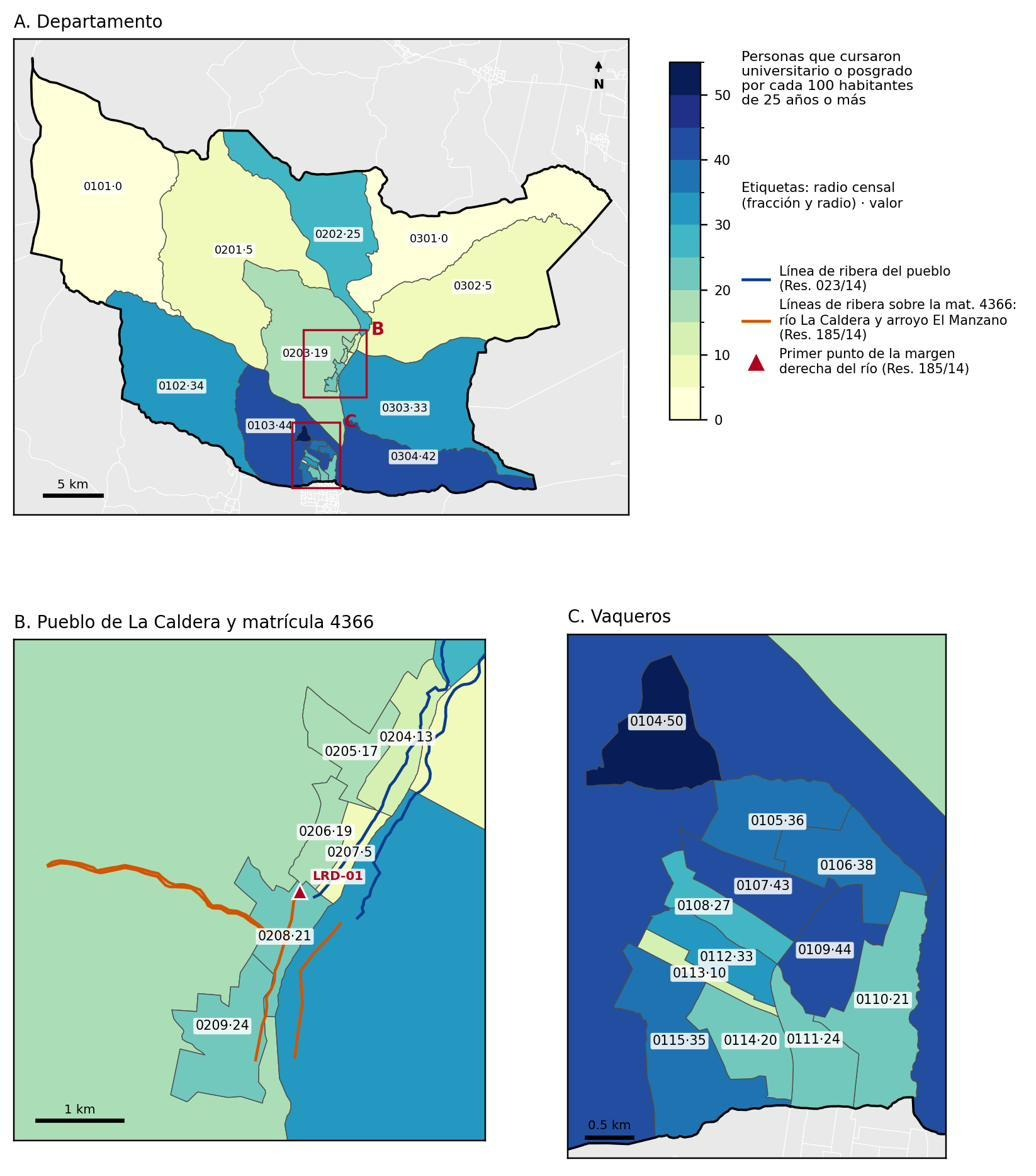
\includegraphics[width=\textwidth,height=0.86\textheight,keepaspectratio]{fig-formacion-radios.png}
\caption[Formación universitaria por radio censal, 2022]{\textbf{Formación universitaria por radio censal, departamento La Caldera, 2022.} A: el departamento; los recuadros B y C marcan los detalles. B: el pueblo de La Caldera y la matrícula 4366, con la línea de ribera del pueblo (Resolución 023/14) y las del río La Caldera y el arroyo El Manzano sobre esa finca (Resolución 185/14), trazadas con sus coordenadas publicadas; el triángulo es el primer punto de la margen derecha del río. C: el área urbana de Vaqueros. En gris, los radios de otros departamentos. Elaboración propia con datos del INDEC (Censo 2022, Redatam) y la cartografía de radios corregida por G.~M.~Rodríguez (CEUR-CONICET, versión 1.0); coordenadas de los edictos de las Resoluciones 023/14 y 185/14.}\label{fig:formacionradios}
\end{figure}

\begin{cautela}
\textbf{Y hay un cruce que este libro tenía en tres capítulos distintos y que conviene hacer acá, porque cambia lo que la fracción 03 significa.}

\begin{center}\small
\begin{tabular}{@{}p{7.6cm}r@{}}
\toprule
Viviendas sin hogar residente & \textbf{43,17\,\%} \textit{(5º de 159 fracciones)} \\
Personas por vivienda & \textbf{1,39} \\
Formación universitaria o de posgrado & \textbf{33,0} por cada cien adultos \\
Hogares sin agua de red \textit{(cap.\ \ref{cap:aguabaja})} & \textbf{58,0\,\%} \\
Población de 15 a 29 años \textit{(cap.\ \ref{cap:ausencias})} & \textbf{14,4\,\%} \\
\bottomrule
\end{tabular}
\end{center}

\textbf{Es el nivel de formación más alto del departamento} ---por encima de Vaqueros, que marca 30,3, y muy por encima del pueblo de La Caldera, que marca 13,6--- \textbf{sobre la peor cobertura de servicios y la mayor proporción de casas vacías.}

Setecientas sesenta y cuatro personas, cuatro de cada diez viviendas sin nadie adentro, 1,4 habitantes por vivienda, seis de cada diez hogares sin agua de red y un tercio de los adultos con paso por la universidad \textbf{no describen un sector rural despoblado}. Describen la segunda residencia de sectores medios y altos que este capítulo tiene por objeto, y que el remate de la casa quinta de Lesser documenta desde 1927.

El capítulo \ref{cap:ausencias} llegó a la misma conclusión por descarte ---«un sector rural de baja densidad con vivienda de fin de semana»--- sin este dato. Con él, la conclusión deja de ser una inferencia sobre lo que falta y pasa a apoyarse en lo que sobra. \textbf{Y ubica el fenómeno}: la vacancia del departamento no está repartida ni concentrada en el pueblo; está en el extremo oriental, sobre la Ruta Provincial 11, que es donde el apéndice \ref{cap:pedidos} ubica los dos fraccionamientos de El Gallinato que el capítulo \ref{cap:opacidad} observa en el visor y que siguen sin identificar.

\textbf{Con la reserva de tamaño de siempre}: son 764 personas y 549 viviendas, y en un universo así un puñado de casos mueve varios puntos. La dirección del hallazgo no depende de eso; su magnitud, sí.
\end{cautela}

\textbf{En Vaqueros}, nueve de los quince radios superan los treinta universitarios por cada cien adultos, y el 0104 llega a cincuenta. Sólo dos quedan por debajo del promedio provincial: el 0113 y el 0101, un radio rural de setenta y ocho habitantes.

\textbf{En el pueblo de La Caldera} la distribución es otra. Los radios del casco oscilan entre 13 y 19, y el más poblado del municipio, el 0207, con 1.279 habitantes, tiene \textbf{5}: menos de la mitad del promedio provincial. Al sur del pueblo, en cambio, los radios 0208 y 0209 marcan 21 y 24, por encima de la capital. \textbf{En el 0209, más de la mitad de los adultos cursó un terciario o una carrera universitaria.}

\textbf{El Durazno está en el 0208 o en el 0209, y la coordenada no permite decir en cuál.} La línea de ribera del río La Caldera sobre la matrícula 4366 ---la finca que el edicto de agua de 2015 vincula con el loteo, aprobado sobre la 6.558--- recorre los dos radios: de los catorce puntos de su margen derecha, publicados en el edicto de la Resolución 185/14, once caen en el 0208 y los tres últimos, río abajo, en el 0209; la del arroyo El Manzano, sobre la misma finca, cruza el 0203 y el 0208. Una versión anterior de este párrafo ubicaba el primer punto en el 0209; trazado con las coordenadas del edicto sobre la cartografía censal, cae en el 0208. El 0208, entre el 0209 y el pueblo, coincide con la ubicación que el Código de Ordenamiento da a El Nogalar y a Potreros de La Caldera, al sudoeste del casco. No es un radio envejecido: el 28 por ciento de su población tiene menos de quince años y sólo el 6 por ciento más de sesenta y cinco.

La lámina \ref{fig:formacioncomparacion} reúne las comparaciones.

\begin{figure}[htbp]
\centering
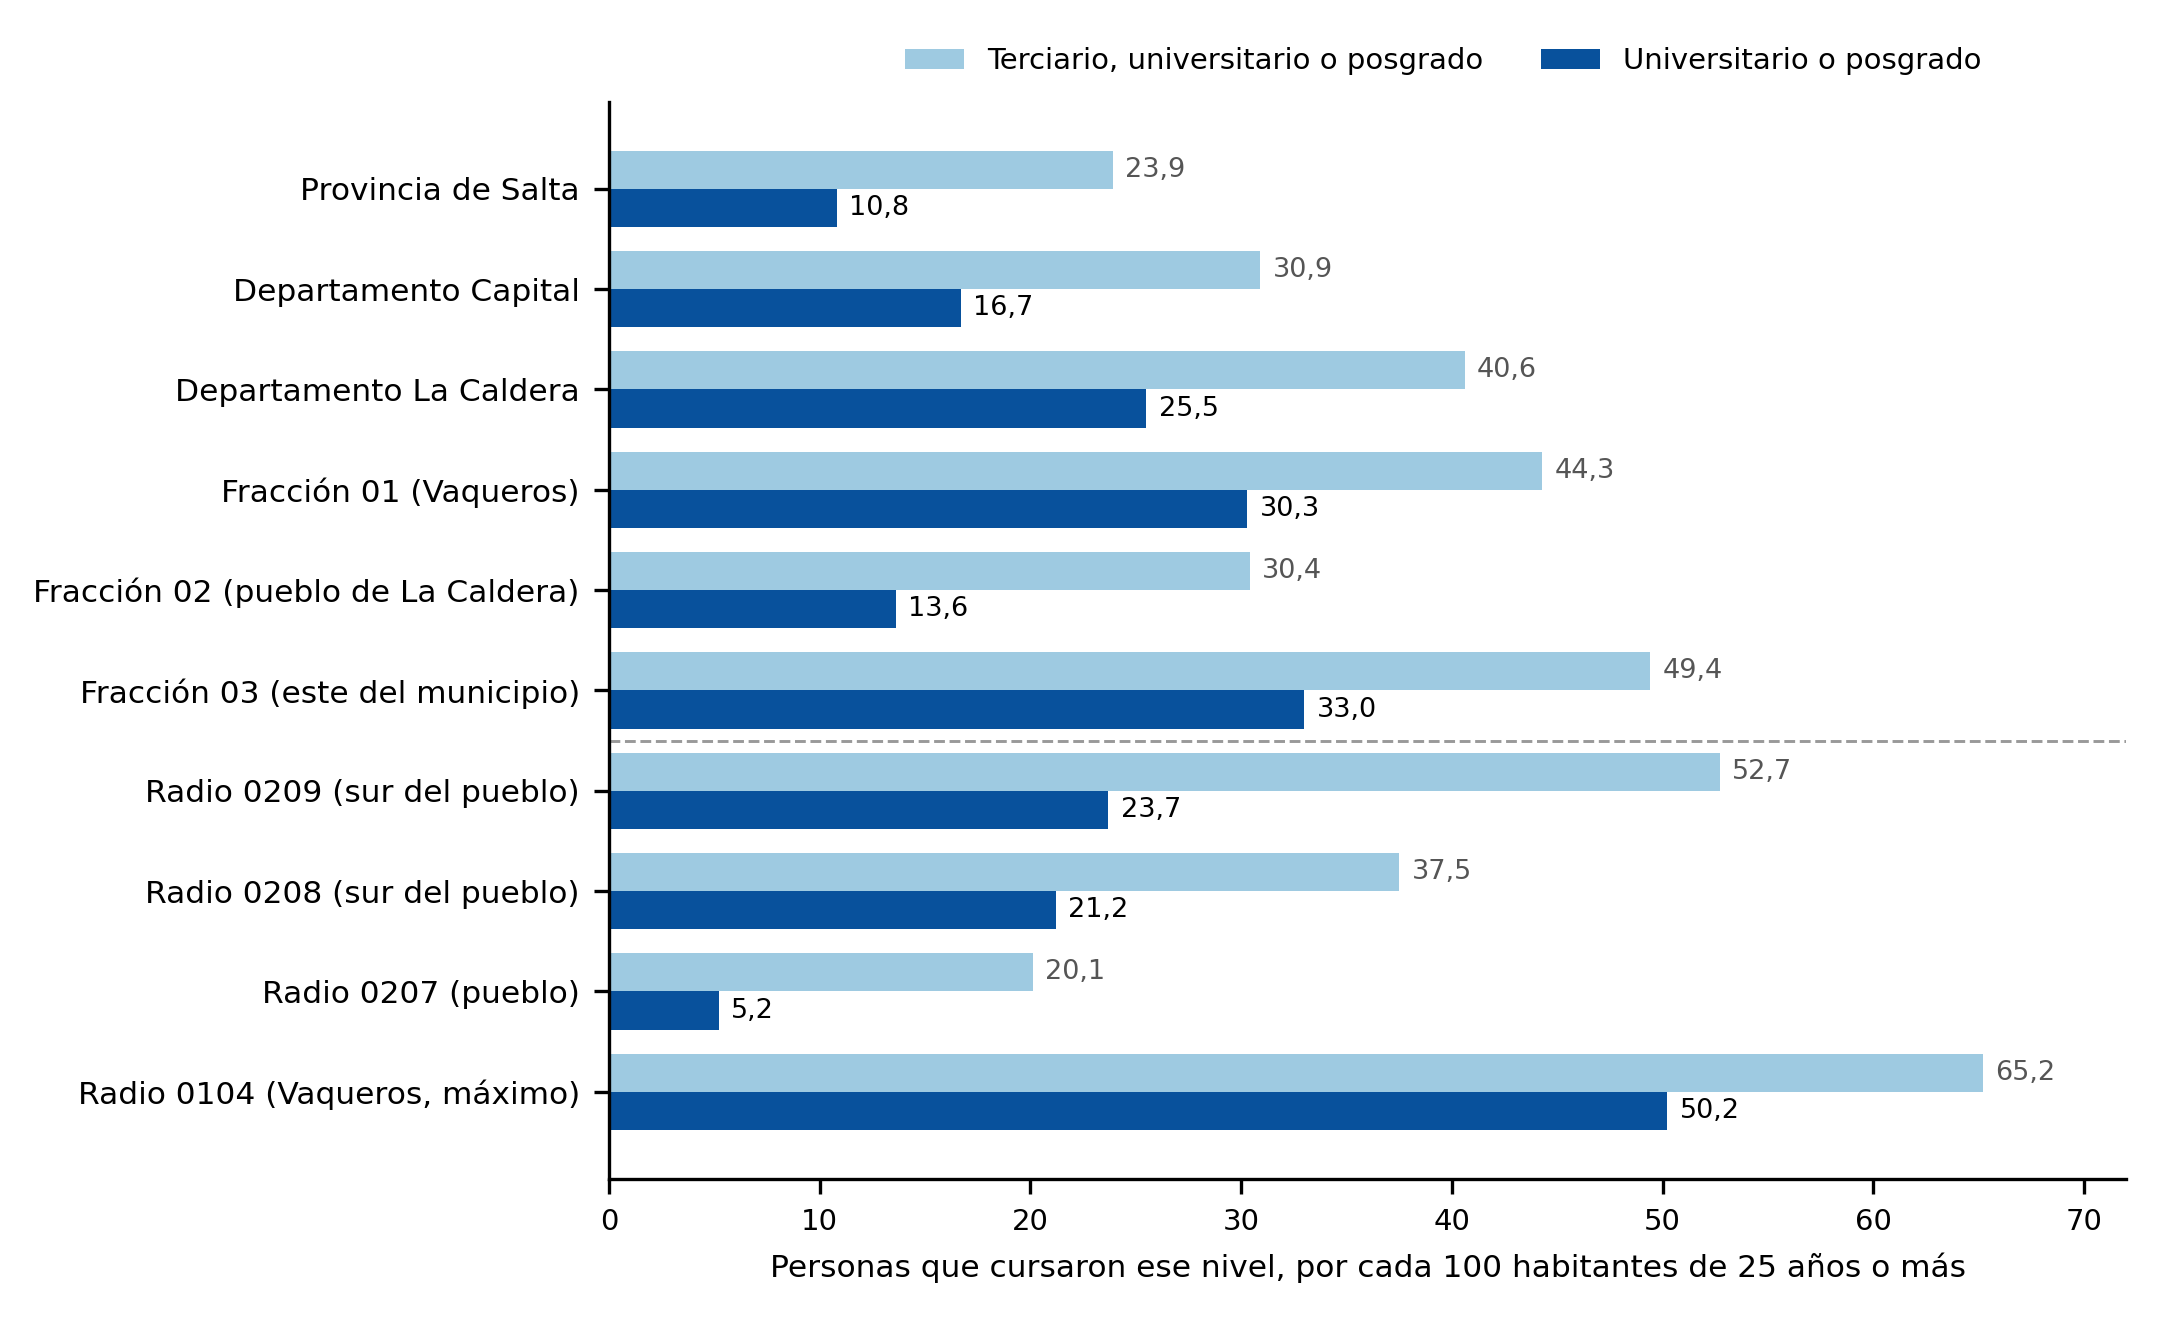
\includegraphics[width=\textwidth]{fig-formacion-comparacion.png}
\caption[Formación por área y radios seleccionados, 2022]{\textbf{Formación por área y radios seleccionados, 2022.} Personas que cursaron cada nivel por cada cien habitantes de veinticinco años o más. Debajo de la línea punteada, las áreas; encima, cuatro radios del departamento. Elaboración propia con datos del INDEC (Censo 2022, Redatam).}\label{fig:formacioncomparacion}
\end{figure}

\begin{cautela}
Cuatro límites, y ninguno es menor.

\textbf{Cursar no es terminar.} La variable registra el nivel más alto al que la persona asistió, no si lo completó. Quien dejó la universidad en primer año cuenta igual que quien se recibió.

\textbf{El indicador es aproximado.} Edad y nivel vienen en el mismo cuadro, pero no cruzados: el numerador incluye a los estudiantes universitarios de dieciocho a veinticuatro años, y el denominador sólo a los mayores de veinticinco. Sirve para comparar áreas entre sí, no como tasa exacta.

\textbf{Los radios son chicos.} El 0209 tiene 150 habitantes y el 0208, 125. Pocas familias mueven mucho el porcentaje. Y en esos loteos buena parte de las viviendas son de fin de semana: sus dueños no se cuentan allí.

\textbf{La identificación de los barrios es una inferencia.} Las coordenadas publicadas muestran que la finca 4366 abarca el 0208 y el 0209, pero ninguna señala el loteo; la ubicación de los barrios descansa en la posición relativa que les da el Código de Ordenamiento. Cuál de los dos contiene a El Nogalar y cuál a Potreros de La Caldera no lo establece este libro.
\end{cautela}

\section{Vacancia y turismo son el mismo uso del suelo}

El 18 de febrero de 2026, el mismo mes en que se aprobó el Plan de Manejo, el municipio de La Caldera publicó un parte sobre el fin de semana de Carnaval.

\begin{ficha}{Parte municipal, 18 de febrero de 2026 --- área Turismo}
Tasa Neta de Ocupación Turística promedio del \textbf{80,9 por ciento}, según datos del Ministerio de Turismo y Deportes de la Provincia, que ubican a La Caldera ``entre los principales municipios de la provincia con más alta ocupación''. En los registros locales se contabilizaron \textbf{cuatro establecimientos con el 100 por ciento} de ocupación y otros con el 80 por ciento.

El intendente destacó que hubo ``alta ocupación de \textbf{cabañas}, algunas al 100 por ciento'', y que el municipio obtuvo dos premios turísticos: uno provincial, con el que ``está creando un nuevo circuito turístico en la zona del dique'', y otro nacional para equipamiento tecnológico.
\end{ficha}

\begin{cautela}
Léanse los dos datos juntos, porque son del mismo municipio, del mismo mes y de la misma superficie.

El municipio de La Caldera tiene la \textbf{tercera menor ocupación por vivienda de la provincia} --- 2,23 personas por vivienda particular contra 3,13 provinciales --- y más de una de cada cuatro viviendas sin residentes permanentes (27,9 por ciento en sus fracciones 02 y 03; una de cada cinco es la cifra del departamento). Y en febrero de 2026 informa, con estadística provincial, una ocupación turística del 80,9 por ciento con establecimientos al tope.

No hay contradicción entre ambas cifras: son la misma cosa vista desde dos oficinas. Un parque construido que está vacío la mayor parte del año y lleno los fines de semana largos no es un parque residencial subutilizado; es un parque de uso intermitente. La estadística de vivienda lo registra como vacancia y la estadística de turismo lo registra como éxito.

\textbf{Con una advertencia que corresponde hacer.} El dato turístico mide plazas de alojamiento comercial --- cabañas, hosterías, establecimientos registrados ---, no viviendas particulares vacías. Son universos distintos y este libro no los confunde: la ocupación del 80,9 por ciento no dice nada directo sobre las viviendas que el censo cuenta como deshabitadas. Lo que en cambio muestra es que existe, documentada por el propio Estado, \textbf{una demanda de uso temporario de suelo residencial en el departamento}, y que el municipio la reconoce como su activo económico y la promueve --- incluido un nuevo circuito en la zona del dique, que es el área que la Ley 4486 expropió en 1972.

Nada de esto es un reproche. Un municipio de cuatro mil quinientos habitantes que encuentra en el turismo una fuente de ingreso hace lo que puede hacer. Lo que este libro registra es que \textbf{la vacancia y el turismo no son dos problemas sino dos nombres del mismo uso del suelo}, y que la política municipal fomenta uno mientras la estadística censal mide el otro, sin que ninguna oficina tenga que mirar las dos cifras a la vez.
\end{cautela}


\subsection*{Y el Estado subsidia la capacidad turística}

El fomento del uso temporario no es sólo discurso municipal. Tiene instrumento provincial, y en el departamento se aplicó.

\begin{ficha}{Decreto Nº 3069 del 14 de octubre de 2014 --- B.O.\ Nº 19.409}
Expediente 136-135.448/2013. Ratifica el Contrato de Promoción Turística suscrito el 24 de septiembre de 2014 entre la Provincia y la firma \textbf{La Caldera S.A.}, en el marco de la \textbf{Ley 6064} de Promoción de la Actividad Turística y su modificatoria 7281.

\textbf{Proyecto:} ``Ampliación Hostería La Caldera'' --- construcción, equipamiento y explotación de \textbf{dos nuevas alas de dormitorios y un Salón de Usos Múltiples}, en inmueble propio de 12.427,13 m², \textbf{matrícula catastral 3.196}, parcela 5, manzana 1, sección D, localidad de La Caldera.

\textbf{Beneficios que el régimen prevé:} exención de todos o algunos de los tributos provinciales vigentes o a crearse, con exclusión de las tasas retributivas de servicios; y entrega de \textbf{certificados de crédito fiscal} aplicables al pago de los impuestos a las Actividades Económicas, a los Sellos y al Inmobiliario Rural.

Firman: Urtubey, Saravia, Parodi, Simón Padrós. \textbf{Los alcances concretos de los beneficios están en el Anexo}, que forma parte del decreto y no se publica en el cuerpo.
\end{ficha}

\begin{cautela}
Tres observaciones.

\textbf{La primera cierra el argumento de este apartado.} La ocupación turística que el municipio celebra en 2026 no creció sola: el Estado provincial la promovió con exenciones impositivas y créditos fiscales. En 2014, mientras los vecinos de la zona alta de Vaqueros esperaban la red de agua y el Ministerio exigía a un club de campo que previera abastecerse en forma privada, la Provincia eximía de tributos a una hostería para que ampliara sus dormitorios.

Ninguna de esas tres decisiones es objetable por separado, y las tres son políticas públicas legítimas. Juntas describen una asignación: \textbf{el Estado subsidió la capacidad de alojamiento temporario del mismo territorio cuya capacidad de alojamiento permanente no lograba dotar de agua}.

\textbf{La segunda es de método.} El decreto ratifica un contrato ``por el cual se fijan los alcances de los beneficios concedidos'', y ese contrato es el Anexo. \textbf{El Anexo no se publica.} Cuánto se eximió, por cuántos años y sobre qué base imponible no consta en el Boletín Oficial: consta en el expediente 136-135.448/2013. Es el mismo patrón que el capítulo \ref{cap:opacidad} describe --- el acto se publica, su contenido operativo no ---, y aquí recae sobre dinero público resignado.

\textbf{La tercera es un nombre.} La beneficiaria se llama \textbf{La Caldera S.A.} y es titular de un inmueble de 12.427 metros cuadrados en el pueblo, matrícula 3.196. Este libro no sabe nada más de ella: ni quiénes la integran, ni desde cuándo, ni qué otros inmuebles posee. Una sociedad anónima que lleva el nombre del municipio donde opera merece, por lo menos, que se busque su legajo.
\end{cautela}

\begin{cautela}
Y no fue un caso aislado. Cuatro meses después, el \textbf{Decreto Nº 463 del 9 de febrero de 2015} ratificó un segundo contrato de promoción turística, suscrito el 29 de diciembre de 2014 entre la Provincia y la firma \textbf{Proyecto 1 S.A.}, para el proyecto \textbf{``Ampliación Hotel La Caldera''}, en un inmueble propio de \textbf{matrícula 3.337}, con una superficie cubierta total de 1.605 metros cuadrados. Expediente 136-34167/2010. Se publicó en el Boletín Oficial Nº 19.485 del 19 de febrero de 2015 y, en lugar del contrato, lleva al pie la leyenda «anexo para su consulta en oficinas de nuestra repartición».

El decreto precisa el encuadre: la inversión entra en el artículo 3º de la Ley 6064 ``ya que corresponde a una \textbf{ampliación de más del 40\% de las existencias}''. Es decir, el beneficio impositivo se otorga a quien amplía en esa proporción lo que ya tiene.

Y la misma firma recibiría, seis meses más tarde, algo más que una exención: por el Decreto 2949 del 24 de agosto de 2015 la Provincia le entregó en \textbf{comodato gratuito por veinte años cuarenta y una hectáreas de tierra fiscal} para construir una cancha de golf de dieciocho hoyos, según se documenta en el capítulo \ref{cap:tierrafiscal}.

\textbf{Dos contratos de promoción turística en cuatro meses, sobre dos inmuebles distintos del mismo pueblo, con dos sociedades distintas.} Eso deja de ser un caso y pasa a ser una política: entre fines de 2014 y comienzos de 2015 el Estado provincial resignó tributos para expandir la capacidad hotelera de La Caldera.

Este libro no la objeta. Fomentar el turismo en un pueblo de cuatro mil quinientos habitantes es una decisión legítima y probablemente razonable.

El reglamento de esa ley ---Decreto 2448/85, B.O.\ Nº 12.356 del 4/12/1985--- permite medir cuánto control previó. Exige para cada solicitud la nómina de socios, la declaración jurada de bienes de los integrantes y el plan de inversiones (art.\ 24); obliga a los beneficiarios a presentar declaraciones juradas anuales bajo pena de caducidad de la exención (art.\ 32); manda a la Dirección Provincial de Turismo verificar el cumplimiento e informar al Ministerio \textbf{cada seis meses} (art.\ 33); y hace perder los beneficios si los bienes promovidos se transfieren, venden o arriendan, o si cambia la razón social sin autorización (art.\ 18). Admite además que los municipios adhieran eximiendo sus propias tasas y derechos de construcción (art.\ 37). De modo que la pregunta que este apartado deja sobre La Caldera S.A. ---quiénes la integran--- tiene respuesta escrita en su expediente de promoción, y la de qué se hizo con lo eximido, en los informes semestrales de Turismo. Si La Caldera adhirió al régimen, además, el pueblo resignó sus propias tasas sobre las mismas obras. Lo que registra es la \textbf{simultaneidad}, que ya no admite ser leída como coincidencia: en el mismo bienio, el Estado eximió de impuestos a dos hoteles, exigió a un club de campo que resolviera el agua por su cuenta, tramitó para otro un derecho permanente sobre un río, y dejó a la zona alta de Vaqueros con camión cisterna.
\end{cautela}


\subsection*{El sistema tarifario ya le puso precio a la vacancia}

El cuadro tarifario de la Compañía Salteña de Agua y Saneamiento aprobado por Resolución 2066/25 del Ente Regulador de los Servicios Públicos, con vigencia desde enero de 2026, contiene una categoría que este libro debe registrar.

\begin{ficha}{Categoría ``Baldío'' --- Cuadro tarifario COSAYSA, enero de 2026}
El cuadro distingue, además de las categorías residencial, comercial e industrial, una categoría \textbf{Baldío}, con cargo fijo propio por diámetro de conexión y precio propio por metro cúbico.

\textbf{Precio del metro cúbico, sólo agua:}
\begin{center}\small
\begin{tabular}{@{}lrr@{}}
\toprule
& \textbf{Residencial} & \textbf{Baldío} \\
\midrule
Zona 1 & \$342,53 & \textbf{\$404,01} \\
Zona 2 & \$258,57 & \textbf{\$330,39} \\
Zona 3 & \$191,58 & \textbf{\$293,76} \\
\bottomrule
\end{tabular}
\end{center}

En las tres zonas el metro cúbico del baldío \textbf{cuesta más} que el residencial: un 18, un 28 y un 53 por ciento más, respectivamente. En cargos fijos, el baldío de trece milímetros supera al residencial de categorías 2 y 3.
\end{ficha}

Hay tres cuestiones que se siguen de este cuadro, y conviene separarlas por grado de certeza.

\textbf{La primera es segura: existe una política tarifaria sobre el suelo no ocupado.} El sistema regulatorio provincial no trata al lote vacío como una ausencia; lo trata como una categoría de usuario, con tarifa propia y más cara que la del vecino que vive allí. Alguien decidió, y el Ente Regulador aprobó, que la conexión que no se usa pague más que la que se usa.

\textbf{La segunda es casi segura: hay un registro.} Para facturar una categoría hay que poder identificarla. La empresa sabe, conexión por conexión, cuáles son baldíos. Ese padrón es la contracara operativa del dato censal que este libro construyó con Redatam: el suelo sin uso no sólo se mide cada diez años por censo: se factura todos los meses. Con una salvedad que corresponde hacer: el baldío tarifario es un \textit{lote sin edificar} con conexión, y la vacancia censal son \textit{viviendas construidas} sin hogar. Los dos padrones miden cosas distintas y no deben sumarse ni tomarse uno por el otro.

\textbf{La tercera es una pregunta abierta, no una afirmación.} Este cuadro rige para el área servida por COSAYSA. La empresa presta servicio en el departamento ---el capítulo \ref{cap:defensas} registra contrataciones suyas con destino a La Caldera y La Calderilla, y el capítulo \ref{cap:amparo} sus captaciones--- e intervino a fojas 68 del expediente de El Durazno; lo que no se sabe es qué parte del ejido cubre. Establecer cuántas conexiones de La Caldera y Vaqueros están categorizadas como baldío --- y cuántas de esas corresponden a los loteos que este libro estudia --- requiere pedirle el padrón a la empresa o al Ente Regulador.

Si ese pedido prospera, el capítulo sobre vacancia deja de apoyarse en una sola fuente decenal y pasa a tener una serie mensual con nombre y dirección. Es, de todos los pedidos pendientes de este libro, el que más cambiaría su capítulo más fuerte.

\chapter{La hacienda de un municipio pobre}

\begin{cautela}
Este capítulo mide lo que el municipio recaudaba. El capítulo \ref{cap:presencia} mide lo otro: qué puso el Estado provincial en el departamento en el mismo período ---qué escuelas, qué comisarías, qué oficinas y qué caminos--- y cuánto costó cada cosa. Los dos se leen mejor juntos, porque la renta de un municipio de tercera categoría sólo dice algo puesta al lado del gasto que otra jurisdicción hacía sobre el mismo territorio.
\end{cautela}


\label{cap:hacienda}

Un municipio de cuatro mil quinientos habitantes que en 2020 declaró no poder pagar los
sueldos de su personal administra hoy el suelo del área metropolitana. Este capítulo
reconstruye de dónde salen sus recursos, cuánto valen los inmuebles sobre los que cobra y
por qué lotear más no le aumenta el presupuesto.

\section{Cuánto recaudaba, en números}

Un decreto de 1938 permite ponerle cifra a esa hacienda que no alcanza.

\begin{ficha}{Decreto Nº 3161 del 10 de octubre de 1938}
Expediente 1117-M. Aprueba el balance de fondos del ejercicio \textbf{1937} de la Comisión
Municipal del Distrito de La Caldera y fija en \textbf{\$283,51} su contribución al fondo de
educación común, sobre la base del \textbf{diez por ciento afectable de la renta municipal}.

Firman Luis Patrón Costas y Víctor Cornejo Arias.
\end{ficha}

Si la contribución es el diez por ciento de la renta afectable, \textbf{la renta municipal de
1937 rondaba los dos mil ochocientos treinta y cinco pesos}. Es una inferencia aritmética y
como tal se la presenta: el decreto no publica el total.

Póngase esa cifra en su serie.

{\small
\begin{longtable}{@{}p{2.2cm}p{4.0cm}p{6.4cm}@{}}
\toprule
\textbf{Ejercicio} & \textbf{Renta municipal} & \textbf{Referencia contemporánea} \\
\midrule
\endhead
1908 & \$1.483,77 & Casi el ochenta por ciento venía de \textbf{vender en licitación} el derecho a cobrar los impuestos \\
1918 & \$3.387,50 \textit{(renta real)} & La calcula el decreto 1.660: cálculo de recursos de \$6.471,44 menos \$3.083,94 de saldo anterior «indebidamente computado», contra un mínimo de \$5.000 para ser municipalidad electiva (capítulo \ref{cap:siglo}) \\
1937 & \textbf{\$2.835} \textit{(inferido)} & Una casa quinta de diez hectáreas se remató en 1927 con base de \$6.000; la fundición de Mojotoro, en 1925, con base de \$222.144 \\
1946 & \$3.068 \textit{(recaudado)} & Recursos «efectivamente percibidos» que el decreto 5276-E de 1947 usa para repartir la coparticipación: al departamento le toca el 0,127 por ciento; a la capital, con \$1.298.124, el 54,116 (capítulo \ref{cap:siglo}) \\
\bottomrule
\end{longtable}}

En veintinueve años la renta municipal no llegó a duplicarse en términos nominales. \textbf{Y
la serie completa dice algo más}: entre 1908 y 1918 la renta más que se duplicó, y entre 1918 y
1946 no creció, sino que bajó. Las cuatro cifras no son del todo comparables ---una es la renta
real que calcula un decreto, otra una inferencia aritmética, otra lo recaudado que declara la
coparticipación---, pero ninguna de esas diferencias alcanza para explicar tres décadas sin
crecimiento nominal. Y seguía
siendo menos de la mitad de lo que valía una sola casa de fin de semana del departamento.

\textbf{Y la partida educativa seguía siendo la primera obligación.} En 1908 el veinte por
ciento adicional al Consejo General de Educación era la mayor erogación fija del ejercicio;
en 1932 el municipio arrastraba deuda por renta escolar atrasada y el decreto que aprobó su
presupuesto le ordenó tramitar el reconocimiento del saldo; en 1938 la contribución se fija
por decreto en el diez por ciento de la renta afectable.

\textbf{Treinta años, tres actos, la misma obligación y el mismo mecanismo}: el municipio
recauda poco, la Provincia le fija cuánto de eso va a educación, y el municipio lo debe.

\subsection*{Lo único que el archivo deja ver del régimen impositivo}

De las ordenanzas de impuestos del municipio no queda un solo artículo en el Boletín. Queda
una consulta, y su respuesta.

\begin{ficha}{Resolución Nº 434 del Ministerio de Gobierno --- Salta, 28 de abril de 1930 --- Expte.\ 637-M-1930}
«Vista la consulta elevada por la H.\ Comisión Municipal de La Caldera, sobre procedencia del
cobro de \textbf{impuestos de degolladura a los abastecedores de la peonada de la construcción
del camino nacional de Salta a Jujuy}»; y considerando que la Ordenanza General de Impuestos de
esa Municipalidad «no acuerda excepción alguna a favor de los referidos abastecedores, así como
tampoco existe Ley que la establezca», que «el impuesto de degolladura es de competencia
municipal» y que «los abastecedores que resisten su pago son comerciantes particulares»:

\textbf{Art.\ 1º.} «Declarar \textbf{procedente} el impuesto de degolladura aplicado por la
Municipalidad de Caldera, a los abastecedores de las cuadrillas de peones que trabajan en el
camino nacional de Salta a Jujuy, \textbf{dentro de la jurisdicción de aquélla}.»

Firma Rafael P.\ Sosa, Ministro de Gobierno. B.O.\ Nº 1.330 del 4 de julio de 1930.
\end{ficha}

Es el único acto de las ediciones leídas en que \textbf{el municipio de La Caldera cobra algo a un tercero
por lo que ocurre en su territorio, y el Estado provincial se lo confirma}. Y el tercero no es
cualquiera: son los proveedores de las cuadrillas que estaban construyendo, dentro del
departamento, el camino nacional a Jujuy ---la obra que el capítulo \ref{cap:infraestructura}
sigue durante todo el período.

Dos cosas se deducen de la resolución, y ninguna está dicha en ella. Que en 1930 existía una
\textbf{Ordenanza General de Impuestos} del municipio con articulado suficiente para que el
Ministerio verificara que no contemplaba excepciones ---de modo que el texto existía y alguien
lo leía---. Y que \textbf{hubo resistencia al pago}: la consulta nace de abastecedores que se
negaban.

\begin{cautela}
La resolución no transcribe ni un artículo de esa ordenanza, ni dice cuánto era el impuesto, ni
cuántos abastecedores ni por cuántas reses. El único contenido tributario municipal que este
relevamiento encontró en cuarenta años de Boletín es, entonces, el \textit{nombre} de un
impuesto y la confirmación de que se podía cobrar.
\end{cautela}

\textbf{Y un año antes, el Estado había autorizado a comprarle el terreno para la casa.} La Ley Nº 11088 de 1929 ---sancionada el 27 de septiembre y promulgada el 2 de octubre--- autoriza
la inversión de \textbf{\$500} para adquirir un terreno en el pueblo de La Caldera destinado a
la \textbf{Casa Municipal}, sin individualizar el terreno ni el vendedor; este libro no encontró el acto de compra. Quinientos pesos: lo mismo que seis años después se presupuestaría para el espigón
de emergencia para que el río no entrara a la calle principal.

\subsection*{Cinco actos seguidos, y ni una cifra}

Entre 1941 y 1945 el Boletín publica cinco actos consecutivos sobre la hacienda de La
Caldera. Los cinco aprueban. Ninguno publica un número.

{\small
\begin{longtable}{@{}p{3.5cm}p{2.1cm}p{5.0cm}p{2.0cm}@{}}
\toprule
\textbf{Acto} & \textbf{Fecha} & \textbf{Qué aprueba} & \textbf{Cifras} \\
\midrule
\endhead
Dto. 3072-G, expte. 1766-M/941 & 29/12/1941 & Balance del ejercicio económico 1940 de la Comisión Municipal & \textbf{ninguna} \\
Dto. 6148-G, expte. 190-M/943 & 14/06/1943 & Ordenanza General de Impuestos \textit{y} Ordenanza de Presupuesto de Gastos y Cálculo de Recursos, ejercicio 1943 & \textbf{ninguna} \\
Dto. 755-G, expte. 1549-M/943 & 30/09/1943 & Balance de la renta municipal del ejercicio 1942, elevado conforme el art.\ 89 de la Ley 68 & \textbf{ninguna} \\
Dto. 2857-G, expte. 6463-M/944 & 19/04/1944 & Cálculo de Recursos y Presupuesto de Gastos, ejercicio 1944 & \textbf{ninguna} \\
Dto. 5786-G, expte. 8266/944 & 12/01/1945 & Presupuesto de Gastos y Cálculo de Recursos, ejercicio 1945 & \textbf{ninguna} \\
\bottomrule
\end{longtable}}

Los cinco decretos tienen la misma estructura: visto, informes de Sanidad y del Consejo
General de Educación, dictamen del Fiscal de Gobierno, un artículo que aprueba, un artículo
que \textbf{devuelve el expediente a la comuna} y la fórmula de cierre. El de 1945 llega más
lejos que los otros cuatro: precisa dónde están los números ---«\textit{que corren a fojas 19 y
20 de las presentes actuaciones}»--- y no los transcribe.

\textbf{Se publica el acto; el contenido operativo queda en un expediente que no se publica.}
Es, ochenta años antes, la estructura que el capítulo \ref{cap:opacidad} describe para los
anexos de línea de ribera y para los contratos de promoción turística. Del régimen impositivo
municipal de La Caldera en 1943 y del monto de su presupuesto en 1944 y 1945, el Boletín no
permite saber absolutamente nada más que el hecho de su aprobación y la fecha.

\begin{cautela}
Las coordenadas de archivo, en cambio, quedan completas, y por eso el apéndice
\ref{cap:pedidos} las incorpora: expedientes 1766-M/941, 190-M/943, 1549-M/943, 6463-M/944 y
8266/944, todos devueltos por el propio articulado a la Municipalidad de La Caldera. El
presupuesto de 1945 está, si existe, en las fojas 19 y 20 del último.
\end{cautela}

\textbf{Y hay una vía por la que las cifras sí salieron a la luz: la deuda.} Lo que los cinco
decretos presupuestarios callan aparece, de a pedazos, en las leyes de crédito suplementario
que la Provincia sancionó en esos mismos años para cubrir renglones impagos del departamento
---entre ellos lo adeudado a la expendedora de rentas fiscales de La Caldera, en las Leyes 586
y 705, y el renglón de la Receptoría en la Ley 605---. \textbf{El municipio no publicaba su
presupuesto, pero la Provincia publicaba lo que había que pagarle a quien cobraba por él.} Es
la misma asimetría que el capítulo \ref{cap:opacidad} describe para el presente: lo que se
publica no es lo que se decide, sino lo que hay que saldar.

\textbf{Y hay un dato que corre en contra de la lectura fácil.} El presupuesto de 1943 se
aprueba en junio, con el ejercicio empezado; el de 1944, en abril; el de 1945, el \textbf{12 de
enero}. La demora se derrumba de cinco meses y medio a menos de dos semanas en tres años ---y
son los años de la intervención federal. La tutela presupuestaria no se ejerció siempre con la
misma lentitud, y quien quiera leer el retraso como medida de desidia tendrá que explicar por
qué el trámite más rápido de toda la serie ocurre bajo un gobierno de facto.

También queda fechado, entre esos mismos actos, un cambio institucional que este libro no
tenía. En junio de 1943 el decreto habla de la «\textit{H. Comisión Municipal del Distrito de
La Caldera}» y de su Presidente; en abril de 1944, del «\textit{Interventor de la Comuna de La
Caldera}». \textbf{El municipio fue intervenido en algún momento entre esas dos fechas}, y el
acto de intervención no está en las mil cuatrocientas noventa ediciones revisadas.

\subsection*{Y en 1980 el presupuesto seguía aprobándose desde afuera}

Cuarenta y ocho años después del decreto que aprobaba el presupuesto de 1932 con el ejercicio
a dos meses de cerrar, el mecanismo seguía funcionando igual.

El \textbf{Decreto Nº 1146} del 15 de agosto de 1980, del Ministerio de Gobierno, Justicia y
Educación, aprueba la \textbf{Ordenanza 028/79} de la Municipalidad de La Caldera, dictada el
27 de julio de \textbf{1979}. Total de recursos igual a total de erogaciones:
\textbf{\$258.178.081}. El mismo Boletín publica el equivalente para Vaqueros.

\textbf{El presupuesto de un ejercicio se aprueba trece meses después de sancionado y se
publica al año siguiente.} En 1932 la demora fue de diez meses; en 1980, de trece. La tutela
presupuestaria que el capítulo describe para 1908, 1922 y 1932 no es un rasgo de aquella
época: sigue vigente medio siglo después.

\textbf{Lo que no sigue una línea es la demora.} Puestos en serie ---1932, diez meses; 1943,
cinco y medio; 1944, tres y medio; 1945, dos semanas; 1980, trece meses---, los plazos suben y
bajan sin tendencia. Lo constante no es el retraso: es \textbf{quién aprueba}. En los cinco
casos, el presupuesto del municipio lo aprueba un decreto del Poder Ejecutivo provincial.

Y hay una comparación que conviene hacer con cuidado. Ese mismo año, la Provincia aprobó tres
obras de encauzamiento en el departamento por quinientos veintisiete millones de pesos ---
\textbf{nominalmente, el doble del presupuesto anual del municipio sancionado un año antes}.

\begin{cautela}
Las dos cifras están en la misma moneda, pero no en el mismo momento: el presupuesto se sancionó en julio de 1979 y las obras se aprobaron en agosto y septiembre de 1980, con una inflación anual que en esos años superó el cien por ciento. En términos reales la relación puede estar cerca de uno a uno, y la comparación debe leerse con esa reserva. Pero no debe leerse como que el municipio «recibió» ese dinero: \textbf{las obras
las contrató, ejecutó y pagó la Provincia}, y el municipio no interviene en ninguna de las
tres resoluciones.

Eso es precisamente lo que la comparación muestra. Sobre el territorio de un municipio cuyo
presupuesto anual era de doscientos cincuenta y ocho millones, se decidieron en tres semanas
intervenciones por más del doble de esa cifra, sin que el municipio fuera parte.
\end{cautela}

\subsection*{Y en 1940 también debía sanidad}

La Resolución Nº 2025 del 29 de mayo de 1940 publica la nómina de municipios deudores de la
Dirección Provincial de Sanidad al 31 de marzo de ese año. En el renglón quince figura
\textbf{La Caldera, con \$951,95}.

Puesta contra la renta municipal inferida para 1937 --- unos dos mil ochocientos treinta y
cinco pesos ---, esa deuda equivale a \textbf{alrededor de un tercio de todo lo que el
municipio recaudaba en un año}.

Y se suma a la anterior. En 1932 el municipio arrastraba deuda por renta escolar atrasada; en
1938 su aporte educativo se fijó por decreto en el diez por ciento de la renta afectable; en
1940 debe casi mil pesos a Sanidad. \textbf{Las dos únicas obligaciones que el archivo
documenta --- educación y salud --- las debía simultáneamente.}

\subsection*{Las rendiciones aparecieron}

El apéndice \ref{cap:pedidos} de este libro reclamaba la rendición de cuentas del ejercicio 1933, que en su
momento se había desglosado del expediente «para ser considerada por separado» y no volvió a
aparecer. Volvió: un decreto del 18 de octubre de 1934, publicado en junio de 1935, aprueba
\textbf{las rendiciones de los ejercicios 1932 y 1933} de la Comisión Municipal de La
Caldera, en los expedientes 1741-M, 1258-M y 1256-M, conforme el artículo 89 de la Ley 68.

Se aprueban \textbf{«con las modificaciones señaladas por la Contaduría del Consejo General de
Educación»}. Firman A.\ Aráoz y Alberto B.\ Rovaletti.

Dos cosas.

\textbf{Quien observa las cuentas del municipio es la Contaduría del Consejo de Educación},
no la Contaduría General de la Provincia. El organismo ante el cual el municipio arrastraba
deuda es el mismo que audita su rendición. No hay nada irregular en eso --- la contribución
educativa era la principal obligación del municipio y el organismo acreedor tenía interés
legítimo en revisarla ---, pero completa el cuadro de dependencia que este capítulo describe.

\textbf{Y la aprobación llega dos años tarde.} Las cuentas de 1932 se aprueban en octubre de
1934 y se publican en junio de 1935. Sumado a que el presupuesto de 1932 se había aprobado
en octubre de ese mismo año --- con el ejercicio a dos meses de cerrar ---, el ciclo completo
es el de una administración que autoriza tarde y controla después.

\textbf{Y las rendiciones siguieron apareciendo, siempre igual.} El barrido continuo de
1935--1945 agrega las de los ejercicios \textbf{1935} y \textbf{1937} ---esta última devuelta
por el Decreto 2155 y aprobada después--- y la de \textbf{1940}, que es a la vez el primero de los cinco actos de la sección anterior. Sumadas a las de 1932 y 1933
y a los cinco actos presupuestarios de la sección anterior, son \textbf{nueve actos sobre la
hacienda de La Caldera entre 1932 y 1945} ---contando por separado las rendiciones de 1932 y 1933, que aprobó un solo decreto---, todos publicados y sólo uno con una cifra: el Decreto 3161/1938, que fija la contribución educativa sin publicar la renta. Lo que el
Boletín deja ver de las finanzas del municipio en trece años es la lista de los expedientes
que las contienen.

\section{El municipio como contratista, en 1933}

Este capítulo documenta que en 2014 la Dirección de Vialidad de Salta contrató directamente
a la Municipalidad de La Caldera para construir badenes, desmalezar banquinas y levantar
gaviones en ocho rutas provinciales, y que ese contrato fue parte de un programa que alcanzó
a nueve municipios el mismo día. La figura tiene ochenta y un años más de los que parece.

\begin{ficha}{Acta Nº 18 del Directorio de Vialidad de Salta, 20 de junio de 1933}
Punto 14: «Resultando muy peligroso el tráfico de carros y jardineras por el \textbf{camino
en cornisa de Salta a Jujuy}, debido al poco ancho de su calzada y a fin de subsanar el
referido inconveniente que perjudica enormemente el transporte de productos de la zona que
atraviesa dicho camino, este Directorio resuelve invertir hasta la suma de \textbf{quinientos
pesos} en la \textbf{limpieza del camino de La Caldera a Tres Cruces por el bajo},
\textbf{encomendando la Dirección de éste trabajo al Presidente de la Municipalidad de La
Caldera D.\ Augusto Regis\index{Regis, Augusto}} quien presentará en su oportunidad toda la documentación
referente a la inversión de los fondos acordados, a cuyo efecto se le remiten las planillas
necesarias.»

Presidencia del Directorio: ingeniero José Alfonso Peralta. Vocales: Domingo Patrón Costas,
Arturo Michel, Sergio López Campo. El acta se publica como anexo del decreto que la eleva a
aprobación del Poder Ejecutivo.
\end{ficha}

El monto es menor. La figura no lo es, y conviene descomponerla.

\textbf{El problema es de la cornisa, y la solución no es la cornisa.} El camino nacional de
Salta a Jujuy es peligroso por angosto; en lugar de ensancharlo, se acondiciona una vía
alternativa por el bajo para descargarlo. Es la misma lógica que el capítulo \ref{cap:defensas} documenta en
1910, cuando la Provincia interviene sobre un camino nacional porque «el Gobierno de la
Nación no tiene votados fondos especiales a este objeto».

\textbf{Y la ejecución se delega en el municipio.} No se hace por administración ni por
contrato con una empresa: se le encomienda al presidente municipal, con planillas y rendición
posterior. En 1933 como en 2014, el municipio es el brazo caminero de una jurisdicción mayor
sobre un camino que no es suyo.

Hay una diferencia, y juega a favor de 1933. El acta nombra a la persona, fija el tope, exige
documentación y remite las planillas. Es decir: hay control de rendición explícito en el
propio acto que asigna. Los contratos de 2014 informan el resultado de una contratación
directa por libre negociación y no publican ni el certificado de obra ni el acta de
recepción, que este libro reclama en el apéndice \ref{cap:pedidos}.

\section{Diez años sin impuestos por plantar olivos}

Los capítulos \ref{cap:poblacion} y \ref{cap:tierrafiscal} documentan que en 2014 y 2015 la Provincia eximió de tributos provinciales a
dos hoteles del pueblo, y que en 2015 cedió cuarenta y una hectáreas fiscales en comodato
gratuito para una cancha de golf. La exención como instrumento de política económica sobre
este departamento tiene ochenta años más.

\begin{ficha}{Ley provincial Nº 145 (numeración original), sancionada el 2 de octubre de 1934}
\textbf{Art.\ 1º:} «Formando parte integrante de la \textbf{región económica del olivo}, los
Departamentos de La Candelaria, Rosario de la Frontera, Metán, Cafayate, Guachipas, San
Carlos, La Viña, Chicoana, Rosario de Lerma, Cerrillos, Capital y \textbf{Caldera}, de acuerdo
con lo establecido por la Ley Nacional Nº 11643, declárase a la Provincia \ldots\ acogida a
los beneficios de la citada Ley.»\par\textit{El 145 es un número de la serie «original» de los años treinta. El Digesto de la Cámara de Diputados reserva «Ley 145» para una ley de 1868 y registra las de esta serie con otra numeración ---la Ley 1340, por ejemplo, como «original 59»---. En la tabla oficial de leyes con doble numeración figura como \textbf{Ley 1423 (orig.\ 145)}, publicada el 12 de octubre de 1934; con ese número hay que pedirla.}

\textbf{Art.\ 2º:} «Quedan \textbf{eximidas por el término de diez años, de todo impuesto
provincial ó municipal, las tierras en que se planten olivos}.»
\end{ficha}

Tres cosas.

\textbf{Hubo un intento de asignarle una vocación productiva al departamento}, por ley y con
beneficio nacional. La Caldera fue incluida en la región económica del olivo junto a otros
once departamentos. El capítulo \ref{cap:tierra} documenta qué quedó de la agricultura departamental
ochenta y cuatro años después: una pérdida del ochenta y ocho por ciento de la superficie
agropecuaria mientras la provincia ganaba. El olivo no está entre lo que se cultiva hoy.

\textbf{La Provincia eximió de impuestos municipales sin intervención del municipio.} El
artículo 2º libera esas tierras de todo tributo provincial \textbf{o municipal} por diez
años. Es decir: una ley provincial resigna la recaudación de un municipio que no la votó, en
un momento en que ese mismo municipio arrastraba deuda escolar y gastaba en sueldos más de
lo que la ley le permitía.

No hay nada excepcional en eso --- las provincias legislan sobre tributos municipales con
frecuencia --- y este libro no lo objeta. Lo registra porque completa el cuadro de la
autonomía: el municipio no decidía su categoría, no aprobaba su presupuesto, no fijaba su
planta, y tampoco controlaba las exenciones sobre su propia base imponible.

\textbf{Y la exención es antigua como técnica.} En 1934 se eximía por plantar olivos; en
2014 y 2015, por ampliar hoteles. El instrumento es el mismo y el destinatario cambió: de
quien produce en la tierra a quien aloja sobre ella. Es, en una sola línea de continuidad
fiscal, el arco que este libro describe.

\section{El presupuesto llegaba tarde y con deuda}

El capítulo \ref{cap:siglo} documenta que en 1922 el Poder Ejecutivo provincial aprobaba por decreto el
presupuesto que la comisión municipal sancionaba. Diez años después el mecanismo seguía
igual, y un decreto permite ver qué significaba en la práctica.

\begin{ficha}{Decreto Nº 15.445 del 28 de octubre de 1932}
Expediente 1392-M, dictado en acuerdo de ministros. Aprueba la Ordenanza General de
Impuestos, el Presupuesto de Gastos y el Cálculo de Recursos elevados por la
\textbf{Municipalidad de 3ª Categoría de La Caldera}, «proyectados para regir durante el
ejercicio económico del presente año 1932».

Previo dictamen fiscal del 12 de agosto e informe de la Contaduría del Consejo General de
Educación del 25 de octubre. No se formula observación alguna.

\textbf{Dos cargas impuestas al municipio:} elevar al Poder Ejecutivo la rendición de cuentas
del ejercicio 1931, conforme el artículo 184 de la Constitución; e \textbf{iniciar ante el
Consejo de Educación la tramitación para establecer el saldo deudor por renta escolar
atrasada}, conforme la ley de emisión de obligaciones de la Provincia.

Firman Aráoz, Rovaletti y García Pinto (h).
\end{ficha}

Dos detalles de ese acto describen la posición del municipio mejor que cualquier
generalización.

\textbf{El presupuesto se aprobó el 28 de octubre para regir durante 1932.} Es decir, con el
ejercicio a dos meses de terminar. Un municipio que recibe la autorización para gastar cuando
ya gastó no planifica: rinde. Y el decreto que lo aprueba deja constancia, en el mismo acto,
de que todavía debía la rendición del año anterior.

\textbf{Y arrastraba deuda escolar.} El municipio no había girado la contribución que le
correspondía al Consejo General de Educación, y el decreto le ordena tramitar el
reconocimiento de ese saldo. La partida existía desde 1908 --- el cuadro de rentas de aquel
año consigna «al Consejo General de Educación, el 20 por ciento adicional, \$200», la mayor
erogación fija del ejercicio --- y veinticuatro años después seguía impaga.

Y al año siguiente el mecanismo se repite con un agregado que importa. El \textbf{Decreto
Nº 16.798}, del 2 de octubre de 1933 y publicado tres meses más tarde, aprueba el
presupuesto municipal del ejercicio 1933 pero deja constancia de una observación fiscal: el
presupuesto de gastos \textbf{contraría el artículo 79 de la Ley Nº 68} ---la Ley Orgánica de Municipalidades, que el Digesto registra hoy como Ley 1349 (apéndice \ref{cap:normativa})---, que prohíbe invertir
más del veinticinco por ciento de la renta en sueldos de empleados administrativos.

Se aprueba igual, «con la modificación señalada en el dictamen fiscal». Y la rendición de
cuentas del municipio se desglosa del expediente «para ser considerada por separado»: ese
trámite separado terminó en el decreto del 18 de octubre de 1934 que se analiza más arriba.

De modo que en 1933 el municipio de La Caldera gastaba en sueldos administrativos más de lo
que la ley permitía, la Provincia lo advirtió y lo aprobó de todas formas. Ochenta y siete
años después, en julio de 2020, ese mismo municipio declaró por escrito que no podía pagar
los sueldos de su personal.

\textbf{No es la misma situación} --- una es exceso de planta sobre renta, la otra es falta
de caja --- pero las dos describen el mismo desajuste estructural: la estructura
administrativa mínima de este municipio nunca entró en su recaudación.

Ninguna de estas cosas es un escándalo administrativo. Son el retrato ordinario de una
hacienda que no alcanza. Pero conviene retenerlas cuando este capítulo llegue a 2020 y
encuentre a ese mismo municipio declarando por escrito que no puede pagar los sueldos de su
personal: la incapacidad de sostener su propia estructura no aparece con el crecimiento
demográfico. Es anterior a él en casi un siglo.


\section{Julio de 2020: el municipio no puede pagar sueldos}

En julio de 2020, empleados municipales de La Caldera cortaron la Ruta Nacional 9 en apoyo de siete trabajadoras cuyos contratos no fueron renovados. Según \textit{Salta 4400}, el intendente informó que los contratos habían vencido en abril, que continuaron trabajando en mayo y junio para no dejarlas sin empleo, y que la situación económica no daba para más: sostuvo que no tenía dinero para recontratarlas y que se encontraba con los números en rojo para pagar los sueldos del resto del personal, porque la coparticipación ya no alcanzaba.

Las trabajadoras atribuyeron la medida a razones políticas y formularon otras imputaciones sobre la composición de las contrataciones. Este libro no las verifica ni las reproduce: retiene del episodio el reconocimiento público, por el propio Ejecutivo municipal, de una situación de insolvencia corriente.

El dato importa por su fecha. En julio de 2020 el municipio declara que la coparticipación no le alcanza para pagar salarios. Cuatro años antes, el municipio vecino lo había dejado escrito en dos decretos: en octubre de 2016 el intendente de Vaqueros promulgó las ordenanzas que mandaban construir una pasarela en el acceso al barrio Villa Sara y una ciclovía en Lesser (Ordenanzas 502/16 y 503/16, Decretos 156/16 y 157/16) aclarando que su ejecución no cabía en el presupuesto de 2017 «dada la magnitud» de las obras y por «la escasa coparticipación que se recibe por un municipio pequeño como el nuestro», y la subordinó a fondos provinciales o nacionales. Cinco años después, el puente peatonal del ingreso a Villa Sara figuraba entre los proyectos de la senadora por el departamento (capítulo \ref{cap:politica}). La Caldera, por su parte, cinco años antes había aprobado un Plan de Desarrollo Urbano Ambiental y estaba por reglamentarlo con un Código de 152 artículos que crea un Órgano Técnico de Aplicación transdisciplinario, un procedimiento de evaluación de impacto ambiental de dieciséis artículos y un régimen de urbanización de quince pasos con certificados sucesivos, control de avance y garantías de obra.

Ese instrumento presupone una capacidad estatal que el municipio, por su propia declaración, no tiene. No se trata de desidia ni de captura: \textbf{el Código de La Caldera fue diseñado para un municipio que no existe}. La Provincia y el Consejo Federal de Inversiones financiaron y asistieron técnicamente la redacción de la norma; nadie financió la estructura que debía aplicarla.

Ésa es la segunda respuesta --- y la más económica --- a la pregunta que abrió el capítulo \ref{cap:cot}. Es también la que menos sirve para una denuncia, porque no tiene responsable individual.

\subsection*{Cuánto vale un lote baldío, según el Estado}

La discusión sobre la base imponible municipal tiene, en un edicto de remate de 2015, una cifra exacta.

\begin{ficha}{Remate judicial --- B.O.\ Nº 19.651 a 19.653, octubre de 2015}
En los autos ``Huaranca Carvajal, Rocío del Valle vs.\ Goitia, Ignacio --- Ejecución de sentencia'', expediente 434.385/13 del Juzgado Civil y Comercial de 6ª Nominación, se rematan:

el cincuenta por ciento indiviso del \textbf{catastro 1411}, sección C, manzana 9, parcela 11 del departamento La Caldera, ``con la base de las dos terceras partes del valor fiscal, \textbf{o sea \$152,88}''; y el cincuenta por ciento indiviso del \textbf{catastro 1412}, parcela 12, con base de \textbf{\$185,48}.

``Ambos inmuebles se encuentran \textbf{baldíos y deshabitados}. Servicios: \textbf{sin conexión de agua corriente ni energía eléctrica}. Estado de ocupación: desocupados.''

Costo de publicación del edicto: \textbf{\$420}.
\end{ficha}

Hágase la cuenta, porque es de una elocuencia que ningún argumento mejora.

La base de remate es dos tercios del valor fiscal. De modo que el valor fiscal completo de esas mitades indivisas era de unos \$229 y \$278; el de los inmuebles enteros, del orden de \$458 y \$556. \textbf{Los dos lotes juntos estaban valuados fiscalmente, en 2015, en poco más de mil pesos.}

\textbf{El aviso que anunció su remate costó \$420.} Publicar la venta de dos lotes urbanos costó, en el Boletín Oficial, cuatro décimos de lo que el Estado dice que valen.

Ahí está, con número, lo que este capítulo viene sosteniendo. El impuesto inmobiliario y las tasas municipales se calculan sobre esa valuación. Un municipio cuya superficie urbana se multiplica en lotes valuados a cuatrocientos o quinientos pesos no aumenta su recaudación por lotear: \textbf{aumenta su superficie a servir sin aumentar su base imponible}. Cada lote nuevo suma obligación de servicio y aporta un tributo calculado sobre una cifra simbólica.

Y la descripción judicial confirma por otra vía lo que el censo mide: baldíos, deshabitados, sin agua ni luz. No es una excepción encontrada a propósito --- es la descripción rutinaria de un martillero sobre dos parcelas cualesquiera del departamento.

\begin{cautela}
Una advertencia sobre el alcance de este dato, porque conviene no estirarlo.

Son \textbf{dos parcelas}, no una muestra. Su valuación puede estar desactualizada respecto del padrón general, puede corresponder a una zona particularmente marginal del ejido, o puede reflejar un revalúo pendiente que después se corrigió. Una valuación fiscal baja tampoco equivale a un valor de mercado bajo: precisamente el desfasaje entre ambos es lo que este libro sospecha.

Lo que la cifra permite afirmar es más modesto y sigue siendo suficiente: que en 2015 existían en el departamento lotes urbanos cuya valuación fiscal era \textbf{de tres cifras}, y que sobre esas valuaciones se liquidan los tributos que financian al municipio. El padrón inmobiliario completo diría si son la regla o la excepción, y es uno de los pedidos que este capítulo formula.
\end{cautela}


\subsection*{Y en 2007 el municipio pagaba para saber qué había construido}

La base imponible no es sólo una cifra: es una información que el municipio no produce.

\begin{ficha}{Decreto Nº 1639/07 --- B.O.\ Nº 17.645, 19 de junio de 2007}
Aprueba las Actas Acuerdo entre la Provincia, por el Ministerio de Hacienda y Obras Públicas, y los municipios de Vaqueros (22/03/2007, intendente Miguel Ángel Alemán), La Caldera (17/04/2007, intendente Héctor Miguel Calabró) y El Galpón, para que la Dirección General de Inmuebles les preste el \textbf{Servicio de Información Catastral}: una base georreferenciada, con relevamiento satelital y aerofotogramétrico, que detecta las mejoras construidas y no declaradas y las valúa.

Obligaciones del municipio: informar la base catastral y tributaria existente, incorporar las superficies edificadas que le informe la Provincia y comunicarle las mejoras que conozca. \textbf{Precio: el 30 por ciento de lo que el municipio recaude de más por las mejoras detectadas}; en el acta de La Caldera, el 15 por ciento hasta que el municipio se incorpore al Plan de Fortalecimiento Tributario Municipal. Plazo anual, prorrogable tácitamente hasta que se dicte una ley que regule el servicio.

Anexo I de las dos actas, con el mismo texto: el plan de entrega de la información se ordenará por la sectorización del plano de Inmuebles, «considerando que \textbf{La Municipalidad no cuenta con Código de Planeamiento Urbano actual}».
\end{ficha}

\begin{cautela}
Tres cosas. La primera es de fecha: en 2007, según actas firmadas por sus propios intendentes, ni La Caldera ni Vaqueros tenían código de planeamiento. Los dos aprobaron su plan en noviembre de 2015 y su código en 2016, el de Vaqueros el 26 de diciembre (capítulos \ref{cap:cot} y \ref{cap:vaqueros}). El ciclo de loteos que este libro documenta empezó antes que cualquiera de ellos.

La segunda es de dependencia. El impuesto inmobiliario urbano es un recurso propio del municipio, pero la valuación la hace la Provincia, y el municipio pagaba con una parte de su propia recaudación para que la Provincia le dijera qué se había construido en su territorio. Es la forma tributaria de la misma asimetría que este capítulo describe: la función es municipal; el instrumento, provincial.

La tercera es una pregunta. Las actas preveían una Unidad de Seguimiento y Control con dos funcionarios por parte, y una ley que regularía el servicio para todos los municipios. Esa ley no aparece: la búsqueda de leyes provinciales por «información catastral» devuelve sólo la Ley de Catastro de 1948 y otras normas ajenas al tema. Si el proyecto no se sancionó, el régimen quedó librado a convenios anuales prorrogables por silencio. Si el servicio se prestó, cuántas mejoras detectó en el departamento y cuánto pagó el municipio por ellas es lo que dirían los informes de esa unidad. \pendiente{informes de la Unidad de Seguimiento y Control del Servicio de Información Catastral para La Caldera y Vaqueros, y destino del proyecto de ley de 2007 en la Legislatura}
\end{cautela}


\subsection*{El municipio como contratista de la provincia}

\begin{ficha}{Contratación directa por libre negociación --- B.O.\ Nº 19.405, 15 de octubre de 2014}
La Dirección de Vialidad de Salta informa el resultado de la contratación directa por libre negociación \textbf{con la Municipalidad de La Caldera}, expediente 33-192.402/2014-0, encuadrada en los arts.\ 13 y 24 de la Ley 6.838. Presupuesto oficial \textbf{\$307.877}. Contrato aprobado por Resolución 1616/2014, desde el 1 de septiembre de 2014 y por \textbf{cuatro meses}.

\textbf{Trabajos:} construcción de \textbf{badenes y alcantarillas}, \textbf{desmontes de zona de camino}, desmalezado de banquinas, limpieza de alcantarillas, desembanque y limpieza de obras de arte, construcción de \textbf{gaviones de piedra, colchonetas y muros de piedra}, cuadrilla y camión.

\textbf{Alcance:} Rutas Provinciales 11, 28, 107-s, 114-s, 115-s, 124-s, 125-s, 150-s, Acceso Norte, Circunvalación Oeste, Centro de Convenciones y caminos vecinales.

En la misma edición se publican contrataciones idénticas con las municipalidades de El Jardín, La Viña, La Candelaria, Apolinario Saravia, Chicoana, El Quebrachal, San Lorenzo y El Bordo. Y la modalidad se repite al año siguiente: por Resolución 0207/2015 la misma Dirección contrató nuevamente al municipio, desde el 5 de enero de 2015 y por cuatro meses, por \$264.815, con el mismo repertorio de tareas más un camión volcador de seis metros cúbicos ``modelo no inferior al año 1986''.

Y no es la única modalidad. Por \textbf{Resolución SOP Nº 729 del 12 de septiembre de 2014} la Provincia adjudicó a la misma Municipalidad de La Caldera, con encuadre en el art.\ 13 inc.\ a de la Ley 6838, la ejecución de la obra ``Construcción de dos aulas y galería'' en el \textbf{Colegio Nº 5045 `Senado Provincial'} de La Caldera, por \textbf{\$625.663,90} y ciento cincuenta días de plazo, con convenio y crédito legal a favor del municipio.
\end{ficha}

\begin{cautela}
Tres lecturas.

\textbf{Es un programa, no una excepción.} Nueve municipios contratados el mismo día por montos casi iguales --- el de La Caldera coincide al peso con el de Chicoana --- indican una política provincial de tercerizar el mantenimiento vial en los municipios, no un acuerdo singular. Este libro no lo objeta: es una forma razonable de sostener caminos secundarios con estructuras locales.

\textbf{Y da una medida de escala.} Entre el mantenimiento vial y la obra escolar, la Provincia canalizó por el municipio más de novecientos treinta mil pesos en cuatro meses de 2014. Para un municipio de cuatro mil quinientos habitantes es un flujo significativo, y no proviene de la coparticipación ni de sus tasas: proviene de \textbf{prestar servicios y ejecutar obra por cuenta del Estado provincial}, con su propia cuadrilla y su propio camión. El municipio no sólo administra: es contratista.

\textbf{Lo tercero es lo que conecta.} Entre los trabajos contratados figuran ``construcción de badenes'' y ``desmontes de zona de camino'', sobre rutas y caminos vecinales del departamento. Son, término por término, las mismas tareas que el municipio informa estar ejecutando con maquinaria pesada en febrero de 2026, diez días antes de la audiencia judicial.

De modo que la capacidad municipal para construir badenes y desmontar zonas de camino \textbf{no es reciente ni improvisada}: existe desde al menos 2014, está financiada por Vialidad provincial y se ejerce por contrato. Eso no dice nada sobre la legitimidad de lo hecho en 2026 --- que este libro no juzga ---, pero descarta una explicación posible: que las obras de 2026 fueran una respuesta improvisada de un municipio sin medios.
\end{cautela}


\subsection*{Y en 2017 seguía siendo contratista de Vialidad}

Este capítulo documenta que en 1933 la Dirección de Vialidad le encomendó al
presidente municipal la limpieza de un camino, y el contrato de 2014
por badenes y gaviones en ocho rutas provinciales. Hay un tercer punto en la serie.

En octubre de 2017, la Dirección de Vialidad de Salta publica \textbf{dos contrataciones
directas con la Municipalidad de La Caldera}, ambas encuadradas en el artículo 13 de la Ley
6.838, por \textbf{\$606.078} y \textbf{\$493.878}: mantenimiento vial en cinco rutas
provinciales, caminos vecinales de la zona y el acceso al Centro de Convenciones, más
provisión de camión y de maquinaria.

En los dos casos la \textbf{cotización es idéntica al presupuesto oficial}, hasta el centavo.
Los plazos son de cuatro y tres meses. Firma el ingeniero Gerardo R.\ Villalba.

\textbf{La serie queda así: 1933, 2014 y 2017.} Ochenta y cuatro años en los que el municipio
es contratado directamente por el organismo vial de otra jurisdicción para mantener caminos
que no son suyos.

Y conviene retener el dato de escala: un millón cien mil pesos en dos contratos, para un
municipio de tercera categoría que tres años después declararía por escrito no poder pagar los
sueldos de su personal. \textbf{La obra vial para terceros no es un ingreso marginal de esta
hacienda: es una de sus fuentes.}

\subsection*{Y en 2019 la ruta 11 la mantenía otro municipio}

\begin{ficha}{Dirección de Vialidad de Salta --- contrataciones con la Municipalidad de El Bordo, 2019}
Tres contrataciones sucesivas para el mantenimiento de las Rutas Provinciales 10-P, \textbf{11-P, tramo «La Calderilla -- El Desmonte»}, y 12-P: desmalezamiento de zona de camino, bacheo con material bituminoso y provisión de camión.
\begin{itemize}[leftmargin=*,nosep]
\item Contratación directa por libre negociación, expte.\ 33-17063/2019, Res.\ Vialidad 251/19: \$776.282,34, tres meses desde el 1/2/2019 (B.O.\ 12/02/2019).
\item Contratación abreviada, expte.\ 33-90807/2019, Res.\ 875/19: \$1.211.028,08, cuatro meses desde el 2/5/2019 (B.O.\ 14/06/2019).
\item Contratación abreviada, expte.\ 33-189497/2019, Res.\ 1214/2019: \$756.887,74, dos meses desde el 1/7/2019 (B.O.\ 16/08/2019).
\end{itemize}
Las dos últimas se encuadran en el artículo 15, inciso a), de la Ley 8072 y en el artículo 40 del Decreto 1319/18.
\end{ficha}

\begin{cautela}
La Ruta Provincial 11 figuraba en 2014 entre las que Vialidad le encomendaba a la Municipalidad de La Caldera, y es la misma que el plano de Chacras del Gallinato desmembra en 2015 (capítulo \ref{cap:loteo}). En 2019, el tramo que arranca en La Calderilla lo mantiene por contrato un municipio de otro departamento, El Bordo, por unos 2,7 millones de pesos en siete meses. Este libro no sabe si La Caldera dejó de ser contratista para esa ruta, si el tramo contratado a El Bordo cruza el departamento o empieza en su límite, ni si hubo en 2019 contratos con La Caldera por otras rutas; los títulos de los avisos de ese año no los muestran. Lo que sí muestran es que el mantenimiento de un camino que nace en el departamento se decide y se paga sin pasar por su municipio.

Una nota de encuadre: el mismo artículo 15 de la Ley 8072 que la Provincia invocó en 2024 para contratar la consultoría del plan de manejo (inciso e, capítulo \ref{cap:amparo}) aparece aquí con otro inciso, el a), para contratar con un municipio. \pendiente{texto del artículo 15 de la Ley 8072 y contratos de Vialidad con la Municipalidad de La Caldera posteriores a 2017}
\end{cautela}

\subsection*{Y una tercera fuente de ingresos: las licencias}

\begin{ficha}{Decreto Nº 1433 del 29 de abril de 2015 --- B.O.\ Nº 19.531}
Expediente 342-39.526/14. Aprueba el Convenio Específico de Distribución del \textbf{Fondo de Cooperación Técnica y Financiera} entre la Provincia --- representada por el Ministro de Seguridad --- y la \textbf{Municipalidad de La Caldera}, representada por su intendente \textbf{Luis Gerardo Mendaña\index{Mendaña, Luis Gerardo}}.

Por ese convenio la Provincia \textbf{cede y autoriza al municipio a percibir directamente el cien por ciento} de los montos que le corresponderían por la venta de formularios del \textbf{Certificado Nacional de Antecedentes de Tránsito}, correspondientes al \textbf{Centro de Emisión de Licencias} de su jurisdicción.

Antecedente: el convenio del 2 de junio de 2010 entre la Agencia Nacional de Seguridad Vial, la Provincia y el municipio, aprobado por Decreto 4257/11, que certificó el Centro de Emisión de Licencias municipal.

\textbf{El convenio} ---el Anexo, vinculado al decreto en la edición web como copia escaneada--- \textbf{se firmó el 10 de marzo de 2014}, más de un año antes de su aprobación. Del valor bruto de cada formulario, el treinta y seis por ciento corresponde a la Provincia y al municipio; la Provincia cede su parte, de modo que el municipio percibe \textbf{todo ese treinta y seis por ciento}, \textbf{con efecto desde la implementación del sistema} y con \textbf{destino exclusivo a seguridad vial} en su jurisdicción. Su vigencia es la del convenio de 2010, y cualquiera de las partes puede rescindirlo con tres meses de aviso.
\end{ficha}

Un municipio de cuatro mil quinientos habitantes tiene \textbf{Centro de Emisión de Licencias de conducir} desde al menos 2010, conectado a los registros nacionales, y se queda con la porción del formulario que corresponde a la jurisdicción, con destino obligado a seguridad vial.

Sumado a lo anterior, el cuadro de recursos del municipio queda así: coparticipación y tasas propias; contratos de mantenimiento vial y obra escolar con la Provincia; y emisión de licencias con retención íntegra del arancel. \textbf{Al menos dos de esas tres fuentes no dependen de su base imponible sino de convenios con el Estado provincial}, y la de licencias, además, sólo puede gastarse en seguridad vial.

Eso matiza --- sin desmentirla --- la afirmación de que la base fiscal del municipio crece en superficie loteada y no en recaudación. Es cierto respecto de las tasas, pero el municipio compensa esa debilidad con ingresos convenidos. Lo que no cambia es la conclusión de fondo: son recursos que no derivan del suelo que administra, y por lo tanto \textbf{más loteo no significa más presupuesto}.



\chapter{Las redes que no están}

\label{cap:redes}
El agua, la cloaca y el gas son el punto donde la conversión de suelo deja de ser una
cuestión de planos. Este capítulo muestra qué proyectos existieron, qué se le exigió a cada
emprendimiento y qué queda hoy: un corredor donde el Estado proyectó redes públicas y
homologó, en los mismos años, abastecimientos privados. Es la forma más concreta en que la
asimetría que enuncia el capítulo \ref{cap:planteo} se vuelve cotidiana.

\section{Lo que hay y lo que falta}

Lo que sigue es el inventario de lo que hay y de lo que falta: qué emprendimientos resolvieron su abastecimiento por cuenta propia, qué obras públicas se proyectaron y en qué estado quedaron.

\subsection*{Un tercer club de campo, y su agua}

\begin{ficha}{Concesión de agua pública --- B.O.\ Nº 19.452 y 19.453, 29 y 30 de diciembre de 2014}
Expediente 34-6147/05. El \textbf{Dr.\ Gonzalo Saravia Echevehere}, administrador judicial en el juicio sucesorio de don \textbf{Adolfo Saravia Valdez}, promotor del loteo \textbf{``Lesser''} a desarrollarse en el \textbf{catastro 1869 del departamento La Caldera}, tiene iniciado trámite de concesión de abastecimiento poblacional a favor de la población que conforma el loteo \textbf{``Finca Lesser''}, ``\textbf{desarrollo urbano realizado bajo la figura de Club de Campo}''.

\textbf{Aguas a captar desde el río Lesser}, en las coordenadas 24° 41' 26,71'' S y 65° 28' 30,00'' O:
\begin{itemize}[leftmargin=*,nosep]
\item \textbf{115 m³ por día} para uso poblacional, \textbf{de ejercicio permanente};
\item un caudal adicional para \textbf{uso recreativo}, \textbf{de ejercicio eventual}.
\end{itemize}

Firma: Dr.\ Rafael Ángel Figueroa, Jefe del Programa Jurídico.
\end{ficha}

Este aviso completa el cuadro que este capítulo venía armando pieza por pieza, y lo completa con una precisión que ninguna de las piezas anteriores permitía.

\textbf{Es el tercer club de campo del departamento} que aparece en el relevamiento, después de Las Vertientes y de Chacras del Gallinato. Con la Urbanización Cerro de Buena Vista, son cuatro desarrollos de baja densidad con trámite documentado entre 2014 y 2015.

\textbf{Y su agua es permanente.} El abastecimiento poblacional de Finca Lesser se capta del río Lesser con carácter de \textbf{ejercicio permanente}, invocando el artículo 66 del Código de Aguas. Compárese con la concesión del Catastro 1700, seis meses anterior: ciento veinte habitantes abastecidos por un pozo perforado, con carácter \textbf{eventual}, porque el artículo 143 declara eventuales todas las concesiones subterráneas sin excepción.

De modo que el mismo Estado, el mismo año y en el mismo departamento tramitó dos derechos de agua para consumo humano con \textbf{jerarquías jurídicas distintas}. La diferencia no está en el destino --- ambos son abastecimiento poblacional --- ni en el número de beneficiarios. Está en la fuente: quien puede captar de un río tiene derecho firme; quien depende de un pozo, no.

Y captar de un río exige lo que un pozo no exige: una fracción con frente sobre el curso, una obra de toma, un estudio y un trámite que en este caso lleva expediente de \textbf{2005}. Es decir, nueve años. \textbf{La permanencia del derecho de agua es, en los hechos, una función de la capacidad de esperar nueve años y de poseer tierra sobre la ribera.}

\begin{cautela}
Dos precauciones sobre este documento.

\textbf{La primera, de lectura.} El caudal consignado para uso recreativo aparece en el aviso con una cifra que, tomada literalmente, resultaría desproporcionada respecto del uso poblacional autorizado en la misma resolución. Es muy probable que se trate de un error de reconocimiento del escaneo o de una unidad mal transcripta. \textbf{Este libro no publica esa cifra} hasta contrastarla contra el original impreso.

\textbf{La segunda, de fondo.} El promotor actúa como \textbf{administrador judicial de una sucesión}. El loteo Lesser se desarrolla, entonces, sobre un acervo hereditario en trámite, y quien gestiona la concesión lo hace por mandato de un juez. Es una figura que este libro no había encontrado hasta ahora y que introduce un actor nuevo en el circuito de conversión de suelo: el juzgado sucesorio. Qué expediente, qué juzgado y con qué autorización se dispuso el desarrollo urbanístico de un bien sucesorio es materia de ese expediente, no de este aviso.
\end{cautela}

\begin{ficha}{Concesión de agua pública --- B.O.\ Nº 19.963 a 19.967, 14 a 21 de febrero de 2017}
Expediente 0090034-263317/2015. El titular registral del \textbf{catastro 4095} del departamento La Caldera gestiona la concesión de uso de agua pública «para abastecimiento de \textbf{630 familias} del Club de Campo \textbf{Las Vertientes--Eco Pueblo}», sito en ese catastro: \textbf{600,48 m³ por día, con carácter permanente}, a derivar de la \textbf{acequia El Alto, margen derecha del río Wierna}. Encuadre: arts.\ 24 inc.\ a), 51, 62, 65, 66, 118 a 125 y 201 del Código de Aguas y Decreto 2299/03. Oposiciones en treinta días hábiles. Firma Silvia F.\ Santamaría como jefa del Programa Fiscalización y Control; edicto del 7 de febrero de 2017.
\end{ficha}

\begin{cautela}
Con esto Las Vertientes, el primero de los clubes de campo de este capítulo, tiene su agua documentada, y la comparación se amplía. Finca Lesser gestionaba 115 metros cúbicos diarios; Las Vertientes, en 2017, más de cinco veces esa cantidad, para 630 familias: unos 950 litros por familia por día. El derecho pedido es permanente y se toma de una acequia del Wierna, el mismo río cuyas márgenes la Provincia determinaba en esos meses (capítulo \ref{cap:ribera}). Y la solicitud es de 2017, tres años después de que Inmuebles aprobara el club con la condición de un «reglamento de condominio con servicio de agua privado» (capítulo \ref{cap:loteo}): el agua que el plano presuponía privada se gestiona después como concesión pública. Cuatro años más tarde, en 2021, los vecinos de la zona alta de Vaqueros reclamaban agua de camión. El aviso no dice si la concesión se otorgó ni con qué caudal. \pendiente{resolución que otorgó o denegó la concesión del expediente 0090034-263317/2015, y relación entre el catastro 4095 y la matrícula 3989 del plano de 2014}
\end{cautela}

\subsection*{Quién firma, once años después}

Las nóminas de autoridades publicadas a fines de 2025 ---la de la estructura de la Jefatura de Gabinete, donde la Decisión Administrativa 569/25 ubica a la Subsecretaría de Recursos Hídricos (capítulo \ref{cap:ribera})--- permiten cerrar un círculo y abrir dos puertas.

\begin{ficha}{Subsecretaría de Recursos Hídricos --- estructura vigente al 30/12/2025}
\begin{itemize}[leftmargin=*,nosep]
\item Coordinador: David Le Favi.
\item \textbf{Dirección General de Cuencas y Política Hídrica}: Jorge Genaro Torres.
\item \textbf{Dirección General de Concesiones Hídricas}: Leandro Bruno.
\item \textbf{Dirección Legal y Técnica: Silvia Fabiana Santamaría\index{Santamaría, Silvia F.}}.
\end{itemize}
En la misma nómina, la \textbf{Secretaría de Tierra y Bienes del Estado} registra a Miriam Esther Ochoa como Directora de Regularización de Tierras Fiscales, Rurales y Urbanas, y a Natalia Macarena Pierola Matos como Directora General de Regularización Dominial.
\end{ficha}

\begin{cautela}
La continuidad es el dato. \textbf{Silvia F.\ Santamaría\index{Santamaría, Silvia F.}} es quien firmó, como Abogada Jefe del Programa Fiscalización y Control, el edicto de junio de 2014 por el que se tramitó la concesión de agua de pozo del Catastro 1700 de La Caldera. Once años y medio después es Directora Legal y Técnica del mismo organismo. Entre una fecha y otra ocurrieron los dos aluviones, el amparo, la condena, la contratación de la consultoría y la aprobación del Plan.

Eso no es un señalamiento personal y este libro no lo formula como tal. Es lo contrario de lo que suele suponerse sobre la administración provincial: en el área hídrica hay memoria institucional disponible, radicada en personas identificables que siguen en funciones. Quien quiera preguntar por qué la línea de ribera se fijó en 2014 y el desborde ocurrió en 2018 no tiene que reconstruir un organismo desaparecido: tiene que escribirle a una dirección que existe.

Y las dos puertas que la nómina abre son literales. La \textbf{Dirección General de Concesiones Hídricas} es la oficina exacta donde vive la nómina de concesiones del departamento que este capítulo pide. La \textbf{Dirección General de Cuencas y Política Hídrica} es donde vive el Plan de Manejo y la planificación de obras que la jueza ordenó presentar por plazos. Ninguno de los dos pedidos tenía hasta ahora destinatario nombrado.
\end{cautela}

\begin{cautela}
Un cambio de rango que corresponde consignar con reservas. Los documentos que este libro cita de 2014, 2021 y 2024 nombran al organismo como \textbf{Secretaría} de Recursos Hídricos, y en 2024 lo ubican bajo el Ministerio de Producción y Desarrollo Sustentable. La nómina de diciembre de 2025 lo nombra como \textbf{Subsecretaría} de Recursos Hídricos, dentro de la Jefatura de Gabinete, aunque la Ley 8.511 asigna los recursos hídricos al Ministerio de Producción y Minería (capítulo \ref{cap:ribera}).

Los edictos del propio organismo fechan el cambio: en julio de 2025 firma la Secretaría y en marzo de 2026 la Subsecretaría (capítulo \ref{cap:ribera}). El descenso de rango está, por lo tanto, acreditado. Lo que el organigrama oficial y la ley de ministerios deben aclarar es si arrastró competencias, presupuesto o planta, y eso sigue siendo pregunta.
\end{cautela}

\subsection*{La región metropolitana existe, pero solo para los colectivos}

Hay una figura legal que reconoce formalmente lo que este libro describe --- que el corredor norte funciona como periferia de la capital --- y que conviene poner sobre la mesa por lo que incluye y por lo que deja afuera.

\begin{ficha}{Región Metropolitana de Salta --- Ley 7.322, en el marco de la Ley 6.994}
Establece la Región Metropolitana de Salta respecto de los \textbf{servicios de transporte por automotor de pasajeros}, propios e impropios, urbanos e interurbanos. La integran los municipios de \textbf{Salta, San Lorenzo, Vaqueros, Cerrillos, Rosario de Lerma, Campo Quijano, La Merced y La Caldera}, más los que el Poder Ejecutivo incorpore en el futuro.

Esos servicios pasan a ser \textbf{competencia provincial}. La \textbf{Autoridad Metropolitana de Transporte} es el organismo de aplicación, con potestades de planificación, organización, regulación, fiscalización y control, y con facultad de dictar los reglamentos sobre recorridos, cupos, permisos, regímenes tarifarios y calidad del servicio.

\textit{Fuente: considerandos de la Resolución A.M.T.\ Nº 376/14, B.O.\ Nº 19.315.}
\end{ficha}

Léase la lista de municipios: es exactamente el conjunto que este libro viene tratando como un área funcional única. El Estado provincial la reconoció, le puso nombre, la sacó de la órbita municipal y le creó una autoridad con poder de policía.

\textbf{Lo hizo para el transporte de pasajeros.} \textit{(Con una salvedad que el apartado sobre el CorInDeS, más abajo, desarrolla: en 2009 los cinco municipios del corredor se constituyeron por convenio como microrregión, con el ordenamiento territorial entre sus fines. Lo que sigue vale para la única figura con ley, organismo y presupuesto.)}

No para el agua, que en Vaqueros se proyecta por localidad y en los clubes de campo se resuelve en forma privada. No para el suelo, cuya aprobación de loteos tramita municipio por municipio. No para el río Vaqueros, que separa dos jurisdicciones y que ninguna de las dos administra en su conjunto. No para los áridos, que se conceden a ambos lados del límite departamental sin autoridad común.

Cuando este libro sostiene que el corredor se gobierna en fragmentos, no está describiendo una imposibilidad institucional ni una laguna del federalismo. \textbf{La provincia sabe construir autoridades metropolitanas cuando decide hacerlo}, y lo demostró con los colectivos. Que no exista una figura equivalente para la cuenca, para el suelo o para el agua no es un problema de diseño constitucional: es una decisión sobre qué se administra en escala metropolitana y qué se deja en escala municipal.

Un dato que aparece de paso en esos mismos considerandos y que conviene guardar. Al evaluar un reclamo del intendente de San Lorenzo, la Gerencia de Transporte del organismo señala que \textbf{no cuenta con datos del último Censo Nacional por localidad, sólo por departamento}, y estima el crecimiento comparando departamentos: Cerrillos habría crecido un 36 por ciento y \textbf{La Caldera un 40}.

La cifra es del orden de la que el capítulo \ref{cap:pdua} consigna para el período 2001--2010. Lo interesante es lo otro: en 2014, un organismo provincial con potestades de planificación reconocía por escrito que \textbf{planificaba sin datos desagregados por localidad}. Es la misma carencia que este libro tuvo que resolver procesando Redatam por su cuenta.

\subsection*{Vaqueros tuvo su obra de agua en 2014}

\begin{ficha}{Resolución SOP Nº 220 del 21 de abril de 2014 --- B.O.\ Nº 19.304 y 19.306}
Expediente 125-120.154/13. Aprueba el proyecto ejecutivo \textbf{confeccionado por la Compañía Salteña de Agua y Saneamiento} y completado por la Dirección de Obras Hídricas y Saneamiento, para la obra \textbf{``Acueducto, Mejoras en Planta Potabilizadora, Canal de Aducción y Redes Maestras --- Localidad Vaqueros''}.

Presupuesto oficial \textbf{\$1.500.000}, modalidad ajuste alzado, plazo de \textbf{ciento ochenta días corridos}. Se autoriza el proceso selectivo con encuadre en el art.\ 10 de la Ley 6838. En el mismo mes se llama a Concurso de Precios Nº 16/2014.
\end{ficha}

\begin{cautela}
Póngase esta obra al lado del reclamo vecinal que este capítulo recoge.

En abril de 2014 la Provincia aprobó el proyecto ejecutivo de un acueducto con planta potabilizadora, canal de aducción y redes maestras para Vaqueros, con un plazo de ejecución de seis meses. En julio de 2021 --- siete años después --- vecinos de la zona alta del mismo municipio se manifestaban tras más de quince años de reclamos porque en sus casas no había agua.

\textbf{Las dos cosas pueden ser compatibles.} Una obra de redes maestras y planta potabilizadora no necesariamente alcanza la zona alta; un acueducto puede mejorar la conducción sin extender la cobertura; y un proyecto ejecutivo aprobado no equivale a una obra terminada. Este libro no sabe si la obra se ejecutó, ni hasta dónde llegó.

Sí sabe que en noviembre de 2023 la zona alta todavía se estaba conectando por etapas. La \textbf{Resolución Nº 855/23 de la Secretaría de Obras Públicas} (B.O.\ Nº 21.605, 5 de diciembre de 2023; expte.\ 125-263.672/21) aprueba la «Optimización red de agua potable --- Vaqueros --- Zona Alta --- Sector III --- Etapa 3»: 1.686 metros de cañería y \textbf{cincuenta conexiones domiciliarias}, con proyecto de Aguas del Norte, \$39.900.254,77 y sesenta días de plazo, adjudicada por contratación abreviada a la propia Municipalidad de Vaqueros. Sus considerandos dicen que esa tercera etapa necesita, para funcionar, que el IPV concluya «el nuevo acueducto en la zona alta» y que el agua de «la Nueva Planta Potabilizadora de Campo Alegre» llegue a una cisterna de 600 m³ en rehabilitación. \textbf{Nueve años después del proyecto de 2014, la red de la zona alta dependía todavía de obras no terminadas.} Y la serie sigue, con la misma forma que las defensas del río (capítulo \ref{cap:defensas}): en enero de 2025 la Resolución 10/25 aprueba el legajo de la «Optimización de redes Vaqueros --- Zona Alta --- Sector 4 --- Etapa I»; en julio, la 367/25 aprueba un convenio de rescisión de la obra «Optimización de redes Vaqueros»; en septiembre, la 482/25 vuelve a aprobar el legajo del Sector 4, Etapa I. \textit{(Esos tres actos se citan por su título en el índice del Boletín; sus textos no se consultaron.)} En 2026, en cambio, la obra se licita a empresas: el «Nexo para abastecimiento de agua potable a Villa Sara y alrededores y redes distribuidoras», con presupuesto oficial de \$744.570.259,64 y ciento ochenta días de plazo, recibe quince ofertas y se adjudica a NECA S.R.L.\ por \$677.541.957,02 (Resolución 404/26, B.O.\ Nº 22.236, 29 de julio de 2026). Entre las ocho desestimadas está la de D.E.S.A.\ Defensa y Encauzamiento S.A., la misma que en 2022 ofertó por el puente sobre el río Vaqueros, por no presentar el certificado de habilitación de su asesor técnico.

Lo que en cambio puede afirmar, y es suficiente para el argumento del capítulo, es que \textbf{la ausencia de red en Vaqueros no se explica por ausencia de proyectos}. Hubo proyecto ejecutivo, presupuesto asignado y llamado a concurso, en el mismo año en que el Estado exigía a un club de campo del mismo municipio que previera resolver el agua \textbf{en forma privada}.

Ese es el hallazgo: en 2014, sobre el mismo territorio y con meses de diferencia, el Estado proyectaba red pública para la localidad y homologaba abastecimiento privado para el emprendimiento. No son políticas contradictorias --- son dos respuestas a dos capacidades de pago ---, y esa simultaneidad es exactamente lo que este libro llama circuitos paralelos.
\end{cautela}

Hubo, al menos, actividad operativa sobre el sistema. En mayo de 2014 la Compañía Salteña de Agua y Saneamiento contrató directamente, por el artículo 13 h de la Ley 6838, el \textbf{alquiler de una retroexcavadora para trabajos en el Acueducto Norte, localidad de Vaqueros}: proveedor Geomix S.R.L., \$10.100 más IVA, expediente 5.836/14. En el mismo mes adquirió rodamientos para bombeo con destino a la localidad de La Caldera, expediente 5.438/14.

Son montos menores y contrataciones de rutina. Se consignan porque acreditan que en 2014 había actividad operativa sobre el acueducto norte en ambos municipios, y porque ese mismo acueducto reaparece en 2019 en el escrito del amparo, a propósito de un desmonte y de una toma de agua no autorizada.

\section{Agua, cloaca y gas: lo que se proyectó y lo que falta}

\subsection*{La única obra de red de agua registrada}

\begin{ficha}{Una obra que sí existe: red de agua de La Calderilla}Registro del sistema nacional de seguimiento de inversión pública, consultado en septiembre de 2026:
\begin{itemize}[leftmargin=*,nosep]
\item \textbf{Denominación:} ``Optimización del servicio de La Calderilla, La Caldera, Salta''. Renovación completa de las redes y de las conexiones domiciliarias de La Calderilla.
\item \textbf{Organismo responsable:} Ente Nacional de Obras Hídricas de Saneamiento (ENOHSA). Jurisdicción beneficiaria: Secretaría de Obras Públicas de Salta. Modalidad: convenio. Código BAPIN 132888.
\item \textbf{Costo estimado:} \$114.372.451.
\item \textbf{Inicio:} 2021. \textbf{Finalización prevista:} 2023.
\item \textbf{Estado:} \textbf{en ejecución. Avance: 47,43 por ciento.}
\end{itemize}
\end{ficha}

Corresponde leer el cuadro por lo que dice y no por lo que sugiere. Dice que la única obra de red de agua registrada para el departamento en el sistema nacional tenía fecha de finalización en 2023 y, tres años después de esa fecha, figura en ejecución con menos de la mitad de avance.

No dice por qué, pero el Boletín provincial da al menos una causa: en octubre de 2024 el Ministerio de Infraestructura aprobó la \textbf{rescisión del contrato} con Norte Áridos S.R.L.\ para la obra «Optimización del servicio de La Calderilla --- nueva red distribuidora» (Resolución 154/24, B.O.\ Nº 21.828; capítulo \ref{cap:cot}). Si el 47,43 por ciento es el avance que quedó congelado con esa rescisión, o si la obra siguió con otro contratista, el registro no lo distingue; tampoco puede descartarse que el porcentaje esté desactualizado, aunque el sitio declara actualización diaria.

Lo que el dato aporta al argumento de este capítulo es de otro orden y no depende de la causa: \textbf{el municipio no controla el ritmo de la única infraestructura de agua que se está construyendo en su territorio}. La obra es de un ente nacional, ejecutada por convenio con la Provincia, sobre una localidad del departamento. La competencia sobre el suelo es municipal; la capacidad de dotarlo de servicio, no.

Ese desacople --- competencia local, capacidad extra-local --- es el mismo que este libro describe para la aprobación de loteos, para el ordenamiento de bosques y para la expansión de la red de gas. Aquí aparece con un número y una fecha de vencimiento.

\subsection*{Las cloacas}

\textbf{Cloacas.} En la audiencia pública por el loteo Lares de la Inmaculada, en abril de 2019, los vecinos plantearon que temían contaminación por la cantidad de familias a instalarse \textbf{en una zona sin cloacas}. El proyecto de ordenanza del Plan de Desarrollo Urbano Ambiental de La Caldera ubica la planta de tratamiento de efluentes, junto con los basurales, entre los equipamientos ``molestos o incompatibles'' que se localizan en zona sub-urbana; y su lista de proyectos complementarios incluye, como pendiente, la conexión de infraestructura hacia la planta depuradora.

\begin{ficha}{Licitación Pública Nº 29/2015 --- B.O.\ Nº 19.532, 5 de mayo de 2015}
Aguas del Norte llama a licitación, en el marco del \textbf{Plan de Obras de Infraestructura Básica de Agua Potable y Saneamiento}, para la obra \textbf{``Redes Colectoras, Colectora Máxima y Planta Depuradora Cloacal --- Vaqueros''}. Expediente 7807/15. Plazo de ejecución: \textbf{ocho meses}. Pliego: \$10.000. Apertura de ofertas: 9 de junio de 2015.
\end{ficha}

\begin{cautela}
La pregunta por el estado de la red cloacal y los proyectos existentes queda parcialmente respondida, y la respuesta es que el proyecto existió y fue completo.

No se trata de una extensión ni de un tramo: la licitación abarca \textbf{redes colectoras, colectora máxima y planta depuradora}. Es un sistema cloacal entero para la localidad, licitado en mayo de 2015, con ocho meses de plazo.

Lo que este libro \textbf{no sabe} es qué ocurrió después: si se adjudicó, si se ejecutó, si se terminó y a qué superficie del ejido alcanzó. Y sabe, en cambio, que cuatro años más tarde los vecinos de un loteo de Vaqueros seguían planteando en audiencia pública el temor a la contaminación ``en una zona sin cloacas''.

Las dos cosas pueden ser compatibles: una planta depuradora con colectora máxima puede servir al casco urbano y no alcanzar a los loteos de la periferia, que son justamente los que crecieron. \textbf{Pero eso es exactamente lo que hay que averiguar}, y con el número de expediente ya no es una búsqueda difusa.
\end{cautela}

\begin{cautela}
Y una circular aclaratoria del 5 de junio de 2015 revela por qué esa obra podía ser más difícil de lo que su pliego sugiere.

Ante consultas de los adquirentes del pliego, el directorio de la empresa aclaró que el ítem ``trámites para servidumbre de paso y acueducto de la obra completa'' debe ser cotizado por los oferentes y ejecutado por la contratista ``en lo que respecta a todos los tramos de la obra completa \textbf{que hayan sido proyectados en terrenos privados}''. Esos trabajos comprenden \textbf{el estudio general de títulos de los terrenos afectados}, la elaboración de los planos de mensura para servidumbre, su presentación y aprobación ante la \textbf{Dirección General de Inmuebles}, y su entrega al comitente.

\textbf{La red cloacal de Vaqueros debía atravesar propiedad privada.} No un tramo puntual: la aclaración habla de ``todos los tramos'' de los cuatro rubros que estén proyectados sobre terrenos privados, lo que sugiere que no eran pocos.

Tres consecuencias.

\textbf{Primera:} el Estado \textbf{transfirió al contratista} la tarea de averiguar quién es dueño de qué. El estudio de títulos --- exactamente el trabajo que este libro no puede hacer porque es arancelado y presencial --- quedó a cargo de la empresa que gane la licitación, y su costo, incorporado al precio de la obra pública.

\textbf{Segunda:} el trazado de la red no lo define la ingeniería sola. Lo define también dónde se consiguen servidumbres. Una colectora máxima que debe negociar paso por fincas privadas termina siguiendo el mapa de la propiedad, no el de la población.

\textbf{Y tercera, que es una hipótesis y como tal se enuncia:} si la obra se ejecutó y no alcanzó a la periferia, la explicación puede no ser presupuestaria ni técnica. Puede estar en las servidumbres. \textbf{Este libro no lo afirma}, porque no sabe si la obra se hizo ni por dónde pasó. Lo señala porque, de confirmarse, sería la demostración más directa de su tesis: la infraestructura pública llega tarde a este corredor porque el suelo se privatizó antes, y ahora hay que pedirle permiso.
\end{cautela}

\subsection*{El gas}

Primero, dónde llega. El Ente Nacional Regulador del Gas publica tres cartografías que permiten responderlo, y las tres dicen lo mismo.

\begin{ficha}{Tres cartografías del ENARGAS sobre el corredor}
\begin{itemize}[leftmargin=*,nosep]
\item \textbf{Atlas provincial}, lámina «Sistema de Transporte y Distribución de Gas Natural de la Provincia de Salta», sin fecha (lámina \ref{lam:gasatlas}). \textbf{Vaqueros figura como ciudad abastecida con gas natural}, en el extremo de un ramal de la malla regional del Valle de Lerma. \textbf{La Caldera no figura}, y al norte de Vaqueros no hay localidad abastecida ni gasoducto hasta el límite con Jujuy. Distribuidora de toda la zona: Naturgy NOA S.A.
\item \textbf{Mapa nacional «Localidades abastecidas con gas distribuido por redes»}, fechado en octubre de 2024 (lámina \ref{lam:gasnacional}). Registra a Vaqueros entre las localidades abastecidas con gas natural a cargo de la distribuidora. La Caldera no aparece.
\item \textbf{Mapa interactivo del ENARGAS}, exportado el 16 de septiembre de 2026 a escala 1:144.448 (lámina \ref{lam:gasvisor}). Muestra un único marcador en el corredor, sobre el área urbana del sur, atravesada por la Ruta 9; ninguno sobre el pueblo de La Caldera ni sobre el embalse.
\item \textbf{Advertencia de los propios mapas:} a esas escalas no se distinguen los barrios dentro de cada localidad abastecida.
\end{itemize}
\end{ficha}

\begin{figure}[p]
\centering
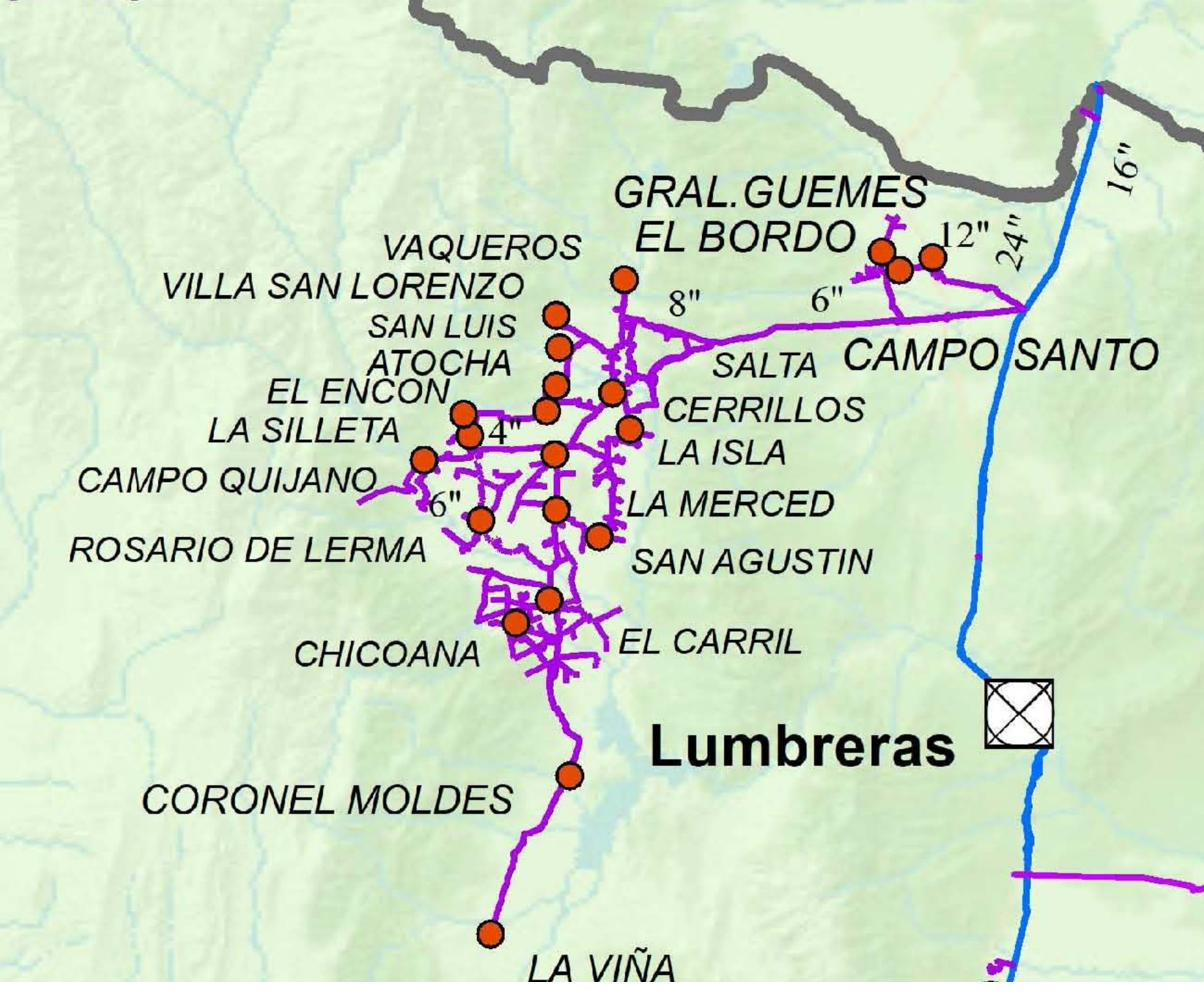
\includegraphics[width=\textwidth,height=0.36\textheight,keepaspectratio]{lam-gas-atlas.jpg}%
\caption[La malla de gas del Valle de Lerma y su extremo norte en Vaqueros]{\textbf{Sistema de transporte y distribución de gas natural, sector del Valle de Lerma.} Los puntos naranja son ciudades abastecidas con gas natural; en violeta, los gasoductos regionales; en azul, el Gasoducto Norte de Transportadora de Gas del Norte S.A.; la línea gris gruesa, al norte, es el límite con Jujuy. \textbf{Vaqueros} es el punto más septentrional de la malla. Entre Vaqueros y ese límite no hay ningún punto: allí está el municipio de La Caldera.}\label{lam:gasatlas}%
\par\vspace{0.3em}%
{\sffamily\scriptsize\color{gris}\raggedright\textbf{Procedencia.}\ ENARGAS, \textit{Atlas provincial del gas}, lámina de la Provincia de Salta, sin fecha, consultada en septiembre de 2026. Recorte del sector central; no se alteró el mapa.\par}%
\vspace{1.4em}
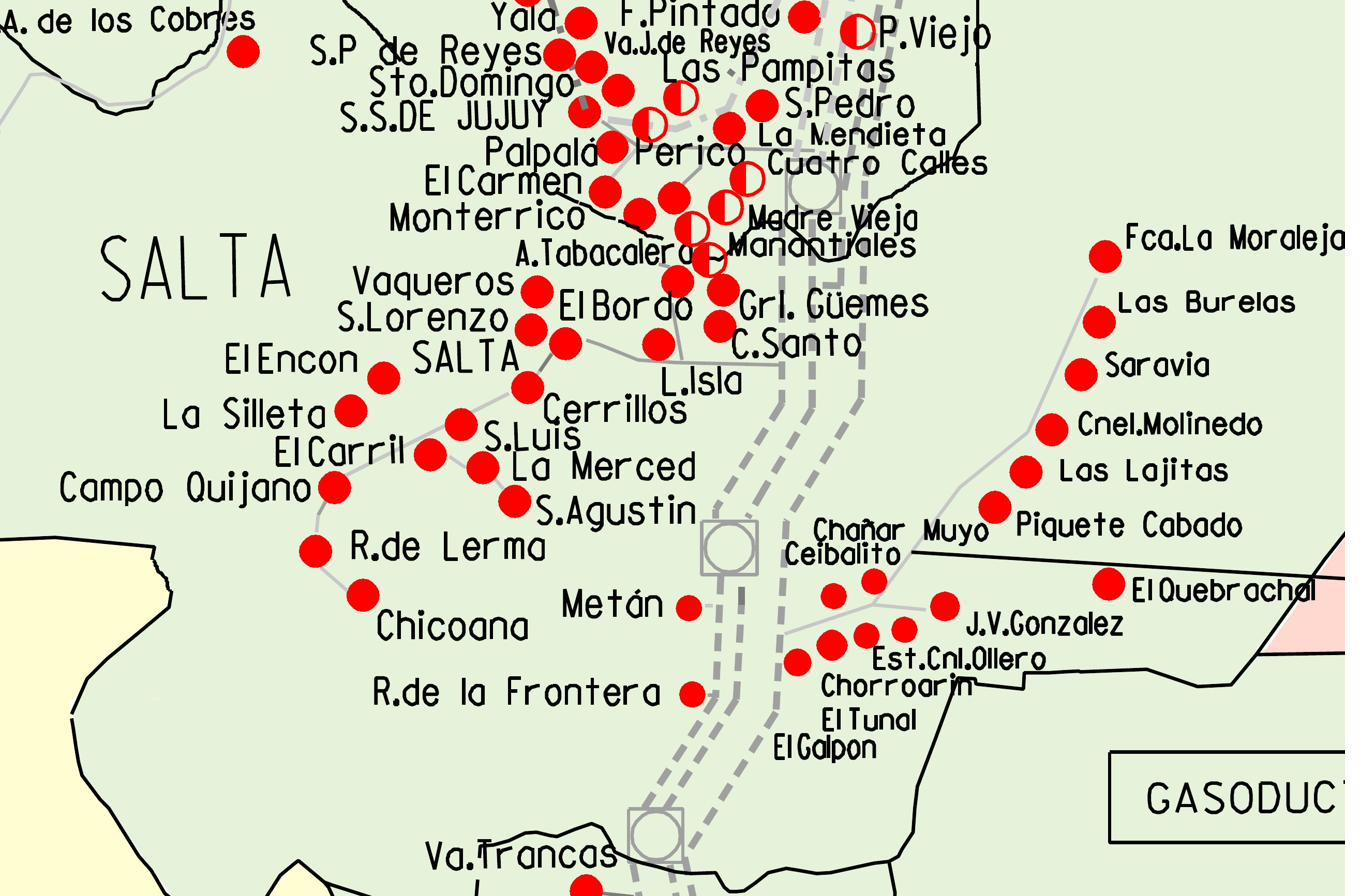
\includegraphics[width=\textwidth,height=0.36\textheight,keepaspectratio]{lam-gas-nacional.jpg}%
\caption[Localidades abastecidas con gas por redes, noroeste, octubre de 2024]{\textbf{Localidades abastecidas con gas distribuido por redes, sector de Salta y Jujuy.} Los círculos rojos llenos son localidades abastecidas con gas natural a cargo de la distribuidora; los partidos, localidades a abastecer con proyectos en ejecución. \textbf{Vaqueros} figura con círculo lleno, junto a San Lorenzo y Salta. \textbf{La Caldera no figura}, ni como abastecida ni como proyecto.}\label{lam:gasnacional}%
\par\vspace{0.3em}%
{\sffamily\scriptsize\color{gris}\raggedright\textbf{Procedencia.}\ ENARGAS, \textit{Localidades abastecidas con gas distribuido por redes. República Argentina}, lámina fechada «ENARGAS -- 10/2024», consultada en septiembre de 2026. Recorte del sector noroeste; no se alteró el mapa.\par}%
\end{figure}

\lamina{lam-gas-visor.jpg}{lam:gasvisor}%
{El corredor en el mapa interactivo del ENARGAS, septiembre de 2026}%
{\textbf{Mapa interactivo del ENARGAS sobre base del IGN, escala 1:144.448.} Arriba, el embalse Campo Alegre; en el centro, sobre el río, el área urbana con el símbolo de cabecera departamental, que corresponde al pueblo de La Caldera; abajo, atravesada por la Ruta 9 y junto al río Mojotoro, el área urbana de Vaqueros. \textbf{El único marcador azul del corredor está sobre Vaqueros.} La exportación no trae leyenda: que el marcador corresponda a la capa de localidades abastecidas es una lectura de este libro, coherente con las dos láminas anteriores, y no una indicación del mapa.}%
{Exportación en PDF del mapa interactivo del ENARGAS (\textit{sig.enargas.gov.ar}), 16 de septiembre de 2026, 7:15. Se recortó el marco del mapa con su fecha y escala; no se alteró el contenido.}

El departamento tiene, entonces, \textbf{un municipio con gas de red y otro sin él}, separados por el río Wierna (Ley 4987; capítulo \ref{cap:cot}). Ninguno de los tres mapas dice hasta dónde llega la red dentro de Vaqueros: si alcanza a los loteos de la periferia y a los clubes de campo, o sólo al casco. Eso se pregunta a la distribuidora y al municipio, y el apéndice \ref{cap:pedidos} lo registra. Lo que sí dicen es que \textbf{la red se detiene en el municipio más cercano a la capital} y no continúa hacia el pueblo que da nombre al departamento.

\textbf{Gas.} El formulario de inscripción para lotes de interés social --- Anexo II de la Resolución 7/16 --- pregunta al solicitante si su vivienda tiene gas y, en caso afirmativo, si es \textbf{de red} o de \textbf{tubo o garrafa}. El Plan Provincial ``Mi Lote'', creado por el Decreto 399/20, promete entregar lotes ``dotados de los servicios públicos esenciales'', y enumera: \textbf{agua, luz eléctrica y apertura de calles}. El gas de red no integra esa enumeración, y las cloacas tampoco.

La enumeración del Decreto 399/20 es el documento más claro sobre el estándar que el Estado provincial se fija a sí mismo. Su programa insignia de urbanización social define los servicios públicos esenciales como agua, luz y calle. Un lote con esas tres cosas cumple la promesa.

Y el formulario de la Resolución 7/16 hace lo mismo que el capítulo \ref{cap:tierrafiscal} documenta para la zona inundable: \textbf{pregunta por el gas de red y el baremo de la Resolución 8/16 no le asigna puntaje}. El Estado registra el dato y no lo usa para decidir.

\subsection*{La ausencia de red no es una imposibilidad legal}

Conviene consignarlo porque cambia el sentido de la carencia.

La Resolución ENARGAS Nº I-910/09, del 9 de octubre de 2009, rigió durante diecisiete años el procedimiento para la expansión de sistemas de distribución de gas. Bajo ese régimen, una obra de ampliación de red podía tramitarse a instancia de la distribuidora, de un subdistribuidor o de \textbf{terceros interesados}, incluidos los futuros usuarios. La metodología definía el Valor de Negocio del proyecto: \textbf{cuando ese valor superaba el monto de la inversión, la obra correspondía íntegramente a la distribuidora}; cuando resultaba inferior, la distribuidora aportaba ese monto y la diferencia la solventaban los usuarios o los terceros interesados, que recibían después una contraprestación --- para los usuarios residenciales, según la Resolución 630/2019, exclusivamente en metros cúbicos de gas.

La distribuidora licenciada para Salta es Naturgy NOA S.A., ex Gasnor S.A., con licencia otorgada por Decreto Nº 2452/92 sobre las provincias de Salta, Jujuy, Tucumán y Santiago del Estero.

\subsection*{El régimen cambió en abril de 2026}

Este apartado se escribió sobre la Resolución I-910/09 y hay que corregirlo, porque esa norma ya no está vigente y porque la corrección abre una vía documental que el libro no tenía.

\begin{ficha}{La secuencia}
\begin{itemize}[leftmargin=*,nosep]
\item \textbf{Res.\ ENARGAS 778/2025}, del 20 de octubre de 2025 (B.O.\ 21/10/2025). No modificó el régimen: \textbf{puso en consulta pública} un proyecto de reglamentación del artículo 16 de la Ley 24.076 --- T.O.\ 2025, por quince días hábiles.
\item \textbf{Res.\ ENARGAS 875/2025}, del 6 de noviembre de 2025. Amplió el plazo por diez días hábiles más, ante requerimientos de los interesados.
\item \textbf{Res.\ ENARGAS 435/2026}, del 24 de abril de 2026 (B.O.\ 27/04/2026). Su artículo 1º aprueba la nueva \textit{Reglamentación de las autorizaciones del Artículo 16 de la Ley Nº 24.076 --- T.O.\ 2025}. Su artículo 2º \textbf{deja sin efecto la Resolución I-910/09 y toda su normativa concordante y complementaria}. Rige desde su publicación; los trámites iniciados antes continúan bajo el régimen anterior.
\end{itemize}
\end{ficha}

La propia resolución enumera tres cambios respecto del régimen anterior: reduce el horizonte de valuación de \textbf{treinta y cinco a diez años}; reemplaza los costos medios derivados de los márgenes tarifarios por costos marginales surgidos de declaraciones juradas, actualizados por una fórmula de mitad índice de precios al consumidor y mitad índice de precios internos al por mayor; y sustituye el flujo de fondos que cada prestadora elaboraba sin estándar por un aplicativo web de uso obligatorio desde la instancia de factibilidad.

\begin{cautela}
El primero de esos cambios importa directamente al corredor. Un horizonte de treinta y cinco años permitía computar como ingreso la demanda de usuarios que todavía no existen; diez años obliga a computar la demanda que madura en una década. Para un tejido de baja densidad, con lotes vendidos y no edificados y con casi una de cada cinco viviendas sin residentes permanentes, ese acortamiento \textbf{endurece el cálculo}: menos consumo computable sobre la misma longitud de cañería.

Dicho de otro modo, el régimen que reemplaza a la I-910/09 hace más difícil, no más fácil, que una expansión hacia La Caldera resulte a cargo de la distribuidora. El libro no puede afirmar que ése haya sido el propósito de la norma, que es de alcance nacional y responde a otra discusión. Puede afirmar que ése es su efecto previsible sobre un parque habitacional con las características que los capítulos anteriores midieron.
\end{cautela}

Y hay un hallazgo documental de otro orden. Los considerandos de la Resolución 435/2026 enumeran a quienes presentaron observaciones durante la consulta pública. Entre ellos figura \textbf{Naturgy NOA S.A.}, con presentación del 27 de noviembre de 2025 en el expediente EX-2025-112087756-APN-GD\#ENARGAS.

Es decir: la distribuidora licenciada para Salta \textbf{tiene posición formal, escrita y pública} sobre la regla que determina quién paga la extensión de red. Este libro venía pidiendo una consulta a la empresa que la empresa no está obligada a contestar. El expediente de la consulta pública es una vía de acceso a esa misma posición que no depende de su voluntad de responder.

De modo que la ausencia de red de gas en el municipio de La Caldera no responde a un impedimento normativo ni a una imposibilidad técnica declarada. Responde a que, hasta donde alcanza este relevamiento, \textbf{nadie solicitó que se calculara el Valor de Negocio del proyecto}. Y ese cálculo es el que determinaría si la obra le corresponde a la distribuidora o si requiere aporte de terceros.

La diferencia entre ``no hay red porque no se puede'' y ``no hay red porque nadie pidió que se evaluara'' es la diferencia entre una carencia y una omisión. Establecer cuál de las dos es requiere consultar al ENARGAS si existen expedientes de expansión para el departamento, y a la distribuidora si evaluó alguna. Ninguna de las dos consultas fue realizada por este libro.

\subsection*{Quién se beneficia de la ausencia}

\begin{cautela}
Corresponde formular la pregunta, y responderla con el mismo criterio que el resto del libro: identificando posiciones estructurales y no intenciones.

\textbf{El desarrollador.} Sin red pública, cada emprendimiento resuelve sus servicios por cuenta propia, y eso deja de ser un costo para convertirse en argumento de venta. Un loteo con vertiente propia vende algo que sus vecinos no tienen. Con red, ese diferencial desaparece. Y hay un efecto adicional sobre el control: el artículo 144 del Código exige garantía de ejecución de obras de urbanización antes de comercializar, pero sin un estándar de red contra el cual medir, ``obras de infraestructura'' es una categoría cuyo cumplimiento nadie puede verificar desde afuera.

\textbf{El propietario no residente de parcela sin edificar.} Es, según el capítulo \ref{cap:poblacion}, un universo identificable, que el municipio intimó en agosto de 2024 por morosidad, y que representa una proporción significativa de un parque con 19,80 por ciento de viviendas sin residentes. Para quien tiene un lote que no habita, la extensión de red no es un beneficio inmediato: es contribución por mejoras y es exposición al gravamen sobre lotes no edificados que ordena el artículo 30 del Código.

\textbf{Nadie decidió esto.} No hay en el material relevado indicio alguno de una decisión de impedir la infraestructura, y el libro no la insinúa. Lo que hay es una configuración en la que la extensión de red no le conviene, en el corto plazo, a ninguno de los actores con capacidad de gestionarla, y le conviene mucho a quienes no la tienen.

Ése es, otra vez, el mismo mecanismo que el capítulo \ref{cap:planteo} enunció: sin red, el único modo de tener servicios es comprar en un emprendimiento que los provea privadamente. El servicio público se convierte en prestación privada y en atributo comercial, y quien no puede pagarlo queda con garrafa, leña y camión municipal dos o tres veces por semana.
\end{cautela}

\section{Agua pública y agua privada}

Este capítulo y el \ref{cap:loteo} discuten qué significa que una concesión sea permanente o eventual. Un
decreto de 1939 introduce una distinción anterior a esa, y más básica: la que separa el agua
sobre la que el Estado decide del agua sobre la que no.

\begin{ficha}{Decreto Nº 2469 del 26 de enero de 1939}
Expediente 632-O. El \textbf{Dr.\ Lucio Ortiz} solicita inscribir en los registros oficiales un
documento firmado por \textbf{Augusto Regis\index{Regis, Augusto}}, Presidente de la Comisión Municipal de La
Caldera, que certifica que la provisión de agua para riego y usos domésticos de la finca
\textbf{«Abra de Lesser»} se hace del \textbf{arroyo del «Abra»}.

\textbf{Se rechaza.} Considerando que, según el propio recurrente, ese arroyo «nace y muere
dentro de la finca» de su propiedad, «no corresponde la inscripción en el Registro Oficial,
ya que \textbf{se trataría de un derecho de uso de agua de dominio privado}» --- y el registro
sólo procede sobre concesiones de agua de \textbf{dominio público}.

Firman Luis Patrón Costas y Carlos Gómez Rincón.
\end{ficha}

\textbf{Primera: hay agua sobre la que el Estado no lleva registro.} Un curso que nace y muere
dentro de un mismo inmueble es, en ese régimen, del dueño del inmueble, y su uso no se
inscribe. De modo que la serie de concesiones que este libro reconstruye --- Urquiza\index{Urquiza, Francisco S.} en 1924,
el pedido denegado de Campo Alegre en 1938, el Catastro 1700 en 2014, El Durazno en 2015, La Misión III en 2015,
Finca Lesser --- \textbf{no es el universo del agua usada en el departamento: es el universo
del agua registrada}. Cuánta se usó sin registro, porque nacía y moría dentro de una finca,
es algo que ningún archivo público puede decir.

Y eso vuelve más pertinente la observación del capítulo \ref{cap:siglo}: si en 1924 el Estado reconoció por
escrito que no había aforado ningún río de la provincia, y si además había cursos enteros
fuera de todo registro, entonces \textbf{nadie estaba en condiciones de saber cuánta agua
había ni cuánta se estaba usando.}

\textbf{Segunda: el certificado lo firmó el presidente municipal.} Para acreditar de dónde saca
el agua una finca privada, el instrumento que se presenta ante la Provincia es una
certificación de Augusto Regis\index{Regis, Augusto}. El municipio no otorgaba derechos de agua, pero certificaba
hechos sobre el terreno, y esa certificación valía como prueba. Es la misma función que en
1938 cumplió su informe en el trámite de Campo Alegre y en 1924 su dictamen en el de Urquiza\index{Urquiza, Francisco S.}.

\textbf{Y ese rechazo no fue el final.} Tres años después, en noviembre de 1942, el mismo
solicitante obtuvo por el Decreto Nº 6705 el \textbf{reconocimiento de derecho exclusivo} de
las aguas del arroyo del Abra, con el mismo fundamento por el cual en 1939 se le había negado
la inscripción: que el arroyo nace y muere dentro de su propiedad.

Lo que en 1939 impedía registrar el derecho --- ser agua de dominio privado --- en 1942 sirve
para declararlo \textbf{exclusivo}. No es una contradicción: son dos actos distintos, uno
sobre el registro y otro sobre el derecho. Pero el resultado práctico merece anotarse.
\textbf{Un curso de agua entero quedó reconocido como de uso exclusivo de un particular, por
decreto del gobernador}, en un departamento donde ochenta años después la zona alta de uno
de sus municipios sigue esperando la red.

\textbf{Y tercera: «Abra de Lesser».} La finca fue deslindada judicialmente en 1938, según un
edicto del mismo corpus, y su nombre remite al partido de Lesser de 1909 y a la casa quinta
de diez hectáreas rematada allí en 1927. En el mismo paraje, en 2005, se iniciaría el
expediente del club de campo «Finca Lesser», que en 2014 gestionaba ciento quince metros cúbicos diarios del río Lesser con carácter permanente.

\section{Y el reparto viene de 1866}

Hay un antecedente anterior a todo lo demás de este capítulo, y aparece en el número 131 del
Boletín, en 1910, dentro de un fallo del Superior Tribunal.

\begin{ficha}{Superior Tribunal de Justicia --- B.O.\ Nº 131, 12 de febrero de 1910}
«\textit{Juicio contencioso-administrativo --- Los señores doña Gumercinda F.\ de Figueroa,
doctor Manuel Landívar y don Antonino Díaz contra el Exmo.\ Gobierno de la Provincia, sobre
\textbf{inconstitucionalidad de la Ley que dota de agua al pueblo de General Güemes}.}»

Los demandantes fundan la acción «\textit{en que la ley de 25 de Setiembre del año 1908 lesiona
sus derechos de propiedad en el caudal de agua del \textbf{Río Mojotoro}, porque al hacerse
efectiva dicha ley ese caudal de agua disminuirá las porciones que tienen adquiridas sobre ella
en virtud de una \textbf{ordenanza municipal de Campo Santo del 18 de Noviembre de 1866},
sancionada como ley por la H.\ Legislatura y promulgada por el Ejecutivo en Enero 27 del
año 67}».

El Tribunal ---doctores Ovejero, Saravia y López, sorteados--- no resuelve el fondo: resuelve
que la acción no es contencioso-administrativa sino demanda ordinaria por inconstitucionalidad,
porque lo atacado es una ley de la Legislatura y no un acto del poder administrador, y que
«\textit{las partes pueden clasificar su acción, por cualquier causa, erróneamente, sin que esto
importe alterar ó cambiar la naturaleza de la causa}».
\end{ficha}

Lo que importa para este capítulo no es el fallo sino lo que la demanda da por sabido.

\textbf{En 1866 una ordenanza municipal repartía el agua del río Mojotoro}, y la Legislatura la
sancionó como ley al año siguiente. \textbf{Diecinueve años antes de la concesión de 1885}, el
mecanismo ya estaba en uso y ya había sido convalidado por la Provincia: el municipio reparte,
la Legislatura ratifica, el derecho queda adquirido. Es exactamente la doctrina que el Decreto
14091 de 1931 pondrá por escrito y que el decreto de 1942 aplicará a la finca «Sausal o
Curuzú».

\textbf{Y en 1908 una ley provincial reasignó ese caudal a otro pueblo}, y los titulares de los
derechos de 1866 fueron a la justicia a defenderlos. \textbf{El conflicto por el agua del
Mojotoro entre quienes la tenían adquirida y un pueblo al que una ley se la da está planteado
en 1908, es decir en el primer año del Boletín.} Veintiuno después, la Ley 1269 dará a Campo
Santo potestad para vigilar y prohibir tomas desde la confluencia; veintitrés después, el
Decreto 14091 mandará investigar todas las concesiones de los dos ríos; y treinta y seis
después, la Provincia concederá cinco litros por segundo a los Ferrocarriles declarando que no
sabe si el río los lleva.

\begin{cautela}
El fallo no nombra a La Caldera. Lo que está en disputa es el caudal del Mojotoro, que se forma
con el Wierna y el de La Caldera, y ninguno de los tres demandantes aparece en el resto de este
relevamiento. \textbf{Las tres fechas normativas ---1866, 1867, 1908--- se transcriben como las
da el fallo} y no fueron contrastadas contra las normas mismas, que este libro no obtuvo.
\pendiente{ordenanza municipal de Campo Santo del 18 de noviembre de 1866, la ley que la
sanciona de enero de 1867, y la ley del 25 de septiembre de 1908 que dota de agua a General
Güemes}
\end{cautela}

\section{El municipio concedía agua en 1885}

El capítulo \ref{cap:planteo} deja abierta una pregunta: cuándo perdió el municipio la voz que tenía sobre el
agua de su jurisdicción. Un decreto de 1942 no la contesta del todo, pero corre el punto de
partida cincuenta y siete años hacia atrás y muestra el mecanismo por el cual esa facultad
cambió de manos.

\begin{ficha}{Decreto Nº 5933 del 24 de abril de 1942 --- Expediente 2462-S}
\textbf{Guillermo Schaefer}, propietario de la finca «Sausal o Curuzú», distrito de Vaqueros,
solicita al Poder Ejecutivo el \textbf{reconocimiento} de los derechos al agua del río
Wierna «otorgado por la \textbf{Municipalidad de la Caldera en el año 1885} al señor Eustaquio
Murúa, antecesor en la posesión de la finca».

Consta, por testimonio del Director del Registro Inmobiliario, que «por \textbf{acuerdo de la
Municipalidad de la Caldera de fecha 4 de junio de 1885} se concedió a don Eustaquio Murúa
el uso de \textbf{treinta litros de agua por segundo} del río Wierna» para riego de esa finca.

El decreto invoca la Ley Orgánica de Municipalidades y el Código Rural vigentes en aquella
época, y reconoce el derecho «sin perjuicio del derecho que pudieran tener otras personas al
uso de dicha agua». Ordena \textbf{inscribirlo en los libros de la Dirección General de Obras
Públicas y del Registro Inmobiliario}.
\end{ficha}

Tres cosas.

\textbf{La primera: el municipio otorgaba concesiones de agua en 1885.} No dictaminaba, no
informaba, no certificaba: \textbf{concedía}. Treinta litros por segundo de un río, por
acuerdo de su propio cuerpo deliberativo, veintitrés años antes de que existiera el Boletín
Oficial de la Provincia.

Eso amplía hacia atrás lo que el capítulo \ref{cap:expropiacion} documenta para 1914, cuando el municipio
reglamentó por ordenanza el reparto íntegro del caudal del río Santa Rufina reconociendo
«derechos adquiridos por uso tradicional». Aquellos derechos tradicionales que la ordenanza de
1914 reconocía podían ser, precisamente, concesiones municipales como ésta.

\textbf{La segunda: el Estado provincial reconoció esa facultad como legítima.} Cincuenta y
siete años después, el Poder Ejecutivo no discute que la Municipalidad de La Caldera pudiera
conceder agua en 1885: verifica el acuerdo, cita las normas que se lo permitían y ratifica el
derecho.

\textbf{Y la tercera es el mecanismo.} El acto no confirma la concesión municipal dejándola
donde estaba: la \textbf{convierte}. La inscribe en los libros de un organismo provincial y
del Registro Inmobiliario. Desde ese momento, el derecho ya no consta en un acuerdo del
municipio sino en un decreto del gobernador y en un registro de la Provincia.

Este libro no puede afirmar que ese haya sido el modo en que el municipio perdió su facultad
--- haría falta la serie completa de reconocimientos y la norma que los ordena, y ninguna de
las dos está en este relevamiento. Pero \textbf{sí puede describir lo que el decreto hace}: un
derecho otorgado por un municipio pasa, por vía de reconocimiento, a existir únicamente en
los registros provinciales. Y en 1942 no fue un caso aislado: ese mismo año el archivo
registra otros dos reconocimientos de derechos de agua en el departamento.

\section{Y en 1931 la Provincia escribió la regla}

Once años antes de ese reconocimiento hay un decreto que enuncia, con las normas en la mano,
de quién era la competencia sobre estas aguas. Es la pieza que faltaba.

\begin{ficha}{Decreto Nº 14091 --- Salta, 23 de octubre de 1931 --- Expte.\ Nº 4920-M}
Dictado por el Interventor Nacional a raíz de una nota de los representantes del Ingenio
Azucarero «La Mendieta» y del Comisionado Municipal de Campo Santo, sobre las dificultades
entre esa Municipalidad y vecinos de Mojotoro por derechos de riego.

Sus considerandos establecen: que los ríos y sus cauces son bienes públicos del Estado (arts.\
2340 inc.\ III y 2341 del Código Civil); que el régimen de concesión está en el art.\ 112 del
Código Rural; y que «\textit{perteneciendo desde un punto de vista más local, a las
atribuciones de las \textbf{Municipalidades de Campaña}, arreglar convenientemente el servicio
y distribución de las aguas de regadío de uso común en sus jurisdicciones respectivas …
estando facultadas para dictar al efecto los reglamentos y ordenanzas correspondientes,
\textbf{mientras no se sancione una ley general de Irrigación}}» (art.\ 56 inc.\ V de la Ley
Orgánica de Municipalidades).

\textbf{Art.\ 1º.} Nombra una Comisión «ad-hoc» integrada por el Director General de Obras
Públicas y Topografía, ing.\ Nolasco F.\ Cornejo, y por los Comisionados Municipales de Campo
Santo y de La Caldera, \textbf{don Pedro Mesple y don Augusto Regis}\index{Regis, Augusto},
encargada «\textit{del estudio e investigación de las concesiones otorgadas a particulares por
el Poder Ejecutivo de la Provincia para el uso-goce de las aguas de dominio público de los
\textbf{Ríos Vaqueros y Wierna}}», de las ordenanzas y reglamentos municipales que reglen su
distribución «\textit{y en general, sobre los usos y costumbres que existan sobre su
aprovechamiento}», con obligación de elevar los antecedentes y un estudio crítico.
\end{ficha}

Cuatro cosas, y ninguna es menor.

\textbf{La regla está escrita, y es la que este libro venía deduciendo.} Hasta que hubiera ley
general de irrigación, la distribución del agua de riego de uso común en cada jurisdicción era
atribución municipal, con facultad de dictar ordenanzas. Eso explica la ordenanza de 1914, la
concesión de 1885 y la competencia que el decreto de 1942 ratifica.

\textbf{Y está fechada por una condición, no por un plazo}: «mientras no se sancione una ley
general de Irrigación». El capítulo \ref{cap:aguabaja} muestra que en \textbf{septiembre de
1944} la Provincia seguía concediendo agua en precario «\textit{hasta tanto entre en vigencia
el decreto ley de agua de la Provincia}». Trece años después, la condición no se había
cumplido.

\textbf{Alguien ordenó investigar todas las concesiones del Wierna y del Vaqueros, en 1931.}
En ese momento el Wierna llevaba, por lo menos, los treinta litros por segundo de la concesión
municipal de 1885 y los cien litros por segundo que el Poder Ejecutivo había otorgado a
Francisco S.\ Urquiza\index{Urquiza, Francisco S.} en 1924 ---y \textbf{ese mismo año de 1931
la Corte de Justicia anuló la revocación de esa concesión}, como consigna el capítulo
\ref{cap:politica}. La comisión debía estudiar exactamente eso.

\textbf{Y el comisionado municipal de La Caldera que integró la comisión es Augusto Regis}, el
mismo que presidirá el municipio durante buena parte de las dos décadas siguientes y será su
comisario de policía en 1942.

\begin{cautela}
\textbf{Este libro no encontró el informe de esa comisión}, ni ningún acto posterior que lo
apruebe, lo rechace o lo cite. No sabe si llegó a reunirse. Lo que el decreto prueba es que en
octubre de 1931 el Gobierno consideró que las concesiones sobre estos dos ríos requerían un
estudio, y que puso a los dos municipios a hacerlo junto con su repartición técnica.
\pendiente{informe y antecedentes de la Comisión ad-hoc del Decreto 14091/1931 sobre las
concesiones de agua de los ríos Vaqueros y Wierna}
\end{cautela}

\textbf{Y encaja con lo que la Legislatura había hecho dos años antes.} En 1929 la Ley 1269 ---original 11078--- había dado a la Municipalidad de Campo Santo potestad para vigilar y prohibir tomas desde la confluencia del Wierna con el de La Caldera; en 1931 el Interventor pone a esa misma Municipalidad, junto con la de La Caldera, a investigar las concesiones de los dos ríos. \textbf{El arreglo institucional no es una autoridad de cuenca: son los municipios, de a dos, mirando el mismo río desde orillas distintas.}

\section{Tres puentes, y los tres viejos}

El capítulo \ref{cap:defensas} documenta que en 1935 los vecinos de La Caldera pidieron a Vialidad un puente
que uniera el pueblo con el camino nacional, y que la respuesta fue que se dispondría lo que
correspondiera «en su oportunidad». Noventa años después, el Plan de Manejo describe así la
conectividad del departamento:

\begin{ficha}{Plan de Manejo, página 113}
«Existen tres puentes; a) el que comunica la localidad de \textbf{Vaqueros con el Departamento
Capital}; b) el que atraviesa el \textbf{río Wierna} comunicando los municipios de Vaqueros y
La Caldera; c) el que permite el \textbf{acceso a La Caldera}. Se trata de infraestructuras
\textbf{antiguas, obsoletas, sin mantenimiento y muy estrechos}.»
\end{ficha}

\textbf{Tres puentes para todo el departamento, y los tres calificados de obsoletos por el
documento que el propio Estado encargó.}

El diagnóstico del Plan agrega que el principal problema del ejido urbano de La Caldera «está
relacionado a la accesibilidad ya que cuenta con \textbf{una única vía de acceso estrecha}», y
que por falta de conectividad este-oeste la mancha urbana crece hacia el sur «mediante un
camino precarizado por la falta de infraestructura hidráulica».

De modo que el corredor por el que este libro sigue la conversión de suelo tiene, en su
extremo norte, \textbf{una sola entrada}. Y el pedido de un segundo puente está hecho desde
1935.

\subsection*{Y en 2022 se licitó el puente}

La «oportunidad» llegó en marzo de 2022.

\begin{ficha}{Licitación del puente sobre el río Vaqueros y la Circunvalación Este, marzo de 2022}
Obra en la \textbf{Ruta Nº 9 --- Circunvalación Este, tramo Salta--La Caldera} ---la cobertura la llama «provincial»; la 9 es nacional---:
desde la rotonda de avenida Bolivia --- «El Quirquincho» --- hasta el \textbf{puente sobre el
río Wierna}, en el kilómetro 1.612 de la ruta nacional 9.

Cuatro kilómetros de carretera ---así en la cobertura; entre la rotonda y el puente del Wierna la distancia es bastante mayor, de modo que uno de los dos datos debe cotejarse con el pliego--- con \textbf{cuatro carriles}, tres rotondas, y un
\textbf{nuevo puente sobre el río Vaqueros} con veredas y ciclovías.

Presupuesto oficial: \textbf{más de mil trescientos cuarenta y un millones de pesos}.

\textbf{Financiada por Vialidad Nacional}; Vialidad de Salta a cargo del proceso licitatorio
y del control de obra.

Tres oferentes: Dal Borgo Construcciones S.R.L.; la unión transitoria de \textbf{DESA --- Defensa
y Encauzamiento S.A.} con Noroeste Construcciones; e Ingeniero Medina S.A.
\end{ficha}

\textbf{Primera: ochenta y siete años después del pedido de 1935 se licita un puente en el corredor, aunque no el que se pidió.} Lo que se licita: el puente de 2022 forma parte de una circunvalación de
cuatro carriles cuyo objeto declarado es dar «más seguridad vial y fluidez al tránsito» entre
la capital y el norte. \textbf{El corredor obtiene un cruce nuevo ---sobre el río Vaqueros, no el que el pueblo pidió--- como efecto de una obra pensada para pasar de largo.}

\textbf{Segunda: la paga Vialidad Nacional.} Es el mismo reparto que el capítulo \ref{cap:defensas} documenta
para 1980, cuando la Nación licitó las defensas de hormigón de la Ruta 9 mientras la Provincia
contrataba por vía administrativa las de los ríos. \textbf{Cuando lo que está en juego es la
traza nacional, aparece el presupuesto nacional.}

\textbf{Y tercera: entre los oferentes está una empresa llamada Defensa y Encauzamiento.} No
es una coincidencia de nombre: DESA es una sociedad anónima salteña, con asamblea convocada
en el Boletín Oficial de 2025, que se presentó en unión transitoria a una licitación de obra
vial sobre el río de este departamento. \textbf{El rubro que da nombre a la empresa es el que
este libro sigue desde 1910.}

\begin{cautela}
\textbf{Y hay una cuarta cosa, que este libro tenía repartida en dos capítulos y no había puesto junta.}

Los tres oferentes de la licitación del puente aparecen, con esa misma razón social o con el apellido de su titular, en el \textbf{cuadro oficial de concesiones de áridos} que la Secretaría de Minería y Energía elevó al juzgado en 2022 (capítulo \ref{cap:resistencias}).

\begin{center}\small
\begin{tabular}{@{}p{3.7cm}p{5.3cm}p{3.2cm}@{}}
\toprule
\textbf{Oferente (2022)} & \textbf{En el cuadro de Minería} & \textbf{Informe de impacto} \\
\midrule
\textbf{Noroeste Construcciones} & «Noroeste Construcciones S.A.», cantera homónima (expte.\ 19.065) & \textbf{No aprobado} \\
Dal Borgo Construcciones S.R.L. & César Domingo \textbf{Dal Borgo}: «La Vaquera» (18.770) y servidumbre de acopio (21.615) & \textbf{No aprobado} (las dos) \\
Ingeniero Medina S.A. & Héctor Enrique \textbf{Medina}: «La Generosa» (16.893) y «Tomasito» (17.049) & \textbf{No aprobado} (las dos) \\
\bottomrule
\end{tabular}
\end{center}

\textbf{Para Noroeste Construcciones S.A.\ no hay cuestión de homonimia}: es la misma razón social, literal, en las dos fuentes. Para las otras dos corresponde la reserva de siempre ---Dal Borgo Construcciones S.R.L.\ no es lo mismo que César Domingo Dal Borgo, ni Ingeniero Medina S.A.\ que Héctor Enrique Medina---, y se resuelve con dos legajos societarios que el apéndice \ref{cap:pedidos} pide.

Lo que queda registrado, y no requiere ninguna inferencia, es esto: \textbf{las tres ofertas presentadas para construir un puente sobre el río coinciden con concesionarios de extracción de áridos del mismo sistema hídrico, y los cinco derechos mineros involucrados ---cuatro canteras y una servidumbre de acopio--- figuran con la evaluación ambiental no aprobada}. Es el cruce de dos nóminas públicas ---un cuadro oficial incorporado a un expediente judicial y la cobertura de una licitación--- y cualquiera puede repetirlo.

Este libro \textbf{no afirma} irregularidad alguna, y hay una lectura enteramente inocua: en un mercado provincial chico, las firmas que tienen movimiento de suelo y áridos son las mismas que se presentan a la obra vial que los consume. Pero es exactamente lo que un vecino planteó en el taller de 2023 y que el capítulo \ref{cap:amparo} transcribe: «\textit{si la misma persona está de los dos lados del mostrador, el medio ambiente no va a mejorar}». La diferencia entre esa frase y este cuadro es que el cuadro tiene números de expediente.
\end{cautela}

\begin{cautela}
Este libro no pudo establecer si esa licitación se adjudicó ni a quién. Que la obra está en ejecución lo indica la prensa de enero de 2026, que informa que la crecida del río Vaqueros arrasó parte del nuevo puente (capítulo \ref{cap:vaqueros}). La preadjudicación estaba prevista para el 31 de marzo de 2022.

Tampoco pudo establecer si DESA participó de alguna de las obras de defensa que el capítulo \ref{cap:defensas}
documenta. \textbf{Que una empresa de ese rubro se presente a una licitación vial en esta
cuenca es un dato; no es una relación probada con ninguna otra obra del libro.}
\end{cautela}

\section{Cuántos hogares, exactamente}

Este capítulo inventaría obras y abastecimientos privados. El censo permite ponerle proporción.

\begin{ficha}{Censo Nacional 2022 --- hogares del departamento sin servicio de red}
\textbf{Sin agua por red pública:} 32,5\,\% en la fracción 66077-01, 17,6\,\% en la 02 y \textbf{58,0\,\%} en la 03.

\textbf{Sin desagüe cloacal conectado a red:} \textbf{más del 95\,\% en las tres}.

Promedio de las cincuenta fracciones de la Capital: 5,8\,\% sin agua y 13,6\,\% sin cloaca.
\end{ficha}

\begin{cautela}
\textbf{El orden de esas tres cifras es el contrario del que el resto del capítulo haría esperar.}

El municipio con gas de red, con proyecto ejecutivo de acueducto, planta potabilizadora y redes maestras aprobado en 2014, y con casi dos tercios de la población departamental ---Vaqueros, la fracción 01--- tiene \textbf{32,5\,\%} de hogares sin agua de red. El pueblo que no tiene ninguna de las tres cosas ---la fracción 02--- tiene \textbf{17,6\,\%}: \textbf{poco más de la mitad}.

No es una paradoja: es la forma exacta del crecimiento que este libro describe. El casco de La Caldera es viejo, chico y está servido; Vaqueros creció por loteos periféricos y de ladera que la red no siguió, y su promedio municipal carga con esa periferia. \textbf{La cobertura no se deteriora donde el Estado no llegó nunca: se deteriora donde el suelo se convirtió más rápido que la cañería.}

Y eso vuelve a poner en su lugar la obra de 2014. Un acueducto con redes maestras para la localidad no alcanza a los loteos que se abren después, ni a los que se abren arriba. La pregunta del apéndice \ref{cap:pedidos} ---hasta dónde llegó esa obra--- deja de ser una curiosidad de expediente: es la que explica un tercio de los hogares de Vaqueros.
\end{cautela}

El detalle y su lectura están en el capítulo \ref{cap:aguabaja}. Acá basta el contraste que da título a este capítulo: \textbf{en el departamento que provee agua a la capital, entre uno de cada seis y casi seis de cada diez hogares no tienen agua de red}, y prácticamente ninguno tiene cloaca.

\section{Septiembre de 2026: una red que sí se extiende}

Este capítulo se llama «Las redes que no están». Conviene cerrarlo con la excepción, que es de
hace días.

\begin{ficha}{Prensa, 5 de septiembre de 2026}
\textbf{«La Caldera: ampliarán la red de agua para cientos de vecinos de barrio Santiago
Apóstol».} Los trabajos comienzan en los próximos días. \textbf{Aguas del Norte} se reunirá con
los vecinos para informar plazos y tareas.
\end{ficha}

\textbf{El barrio Santiago Apóstol es el del capítulo \ref{cap:amparo}}, y la obra la ejecuta la
misma prestadora cuyo convenio sobre la Zona de Exclusión el capítulo \ref{cap:resistencias}
encuentra caducado en 2022.

\begin{cautela}
\textbf{Es una nota de prensa y este libro la consigna como tal}: acredita el anuncio, no la
obra. No tiene expediente, ni monto, ni plazo, ni cantidad de conexiones ---«cientos de
vecinos» no es una cifra---.

Pero registra algo que este capítulo debe registrar por honestidad: \textbf{la red se está
extendiendo}. Lo que el capítulo documenta es que durante décadas no se extendió, no que sea
imposible que se extienda.

\textbf{Y deja la pregunta que importa}: si el barrio Santiago Apóstol recibe red en 2026, qué
pasó entre su aprobación y hoy, y qué barrios y parajes siguen sin ella.
\end{cautela}

\section{La única autoridad metropolitana tiene fecha}

Este capítulo y el \ref{cap:aguabaja} sostienen que la provincia sabe crear figuras metropolitanas cuando
decide hacerlo, y que la única que construyó para este corredor es la del transporte de
pasajeros. Ahora esa afirmación tiene fecha y expediente.

En enero de 2002, la Secretaría de Transporte y Servicios Públicos llama a \textbf{Licitación
Pública Nacional Nº 01/02} para la «concesión del \textbf{corredor metropolitano de
transporte} regular de pasajeros entre localidades de los departamentos \textbf{Capital, La
Caldera y Cerrillos}».

El pliego cuesta \textbf{seis mil pesos} y se vende en dos lugares: el Centro Cívico Grand
Bourg y la Casa de Salta en Buenos Aires. La apertura se fija para el 28 de febrero.

Tres cosas conviene retener.

\textbf{La concesión del corredor existe desde 2002 y agrupa exactamente a los tres departamentos del aglomerado.} La autoridad vino dos años después. La Ley 7322 ---sancionada el 21 de octubre de 2004 y promulgada con veto parcial por el Decreto 2593 del 8 de noviembre de ese año--- estableció la Región Metropolitana de Salta para el transporte de pasajeros, integrada por los municipios de Salta, San Lorenzo, Vaqueros, Cerrillos, Rosario de Lerma, Campo Quijano, La Merced y La Caldera; creó la Autoridad Metropolitana del Transporte como ente autárquico, con potestades de planificación, regulación y control, y creó la sociedad prestadora SAETA. El número del decreto de promulgación lo confirman las resoluciones de la propia Autoridad publicadas en el Boletín Oficial; la fecha de sanción y la edición del Boletín (Nº 17.004) se tomaron de una transcripción del texto de la ley. De modo que en 2002 la escala metropolitana era todavía una concesión; en 2004 pasó a ser una autoridad con competencia sobre los dos municipios de este departamento. No es una construcción reciente ni improvisada: es una concesión licitada a
escala nacional, con pliego, plazos y apertura pública.

\textbf{El pliego cuesta seis mil pesos.} Póngase esa cifra al lado del encauzamiento del arroyo Urquiza que el capítulo \ref{cap:defensas} documenta para noviembre de 2001, todavía en pesos convertibles: el derecho a \textit{ofertar} por el corredor de transporte valía casi lo mismo que \textit{encauzar} un arroyo del departamento.



\begin{ficha}{Decreto Nº 4354/09 --- B.O.\ Nº 18.207, 14 de octubre de 2009}
Aprueba el Convenio de Cooperación para la creación del \textbf{Corredor Intermunicipal para el Desarrollo Sustentable (CorInDeS)}, firmado en julio de 2009 por los intendentes de La Caldera (Héctor Miguel Calabró), Vaqueros (Miguel Ángel Alemán), San Lorenzo (Ernesto Fernando Gonza), San José de los Cerrillos (Humberto Rubén Corimayo) y Salta (Miguel Ángel Isa), y por el gobernador Urtubey «como manifestación de interés». Marco: la cooperación descentralizada con la región francesa Champagne-Ardenne, declarada de interés provincial por el Decreto 2813/09 (B.O.\ Nº 18.145, 14/07/2009). Ese decreto describe el trabajo previo: un acta acuerdo de los cinco intendentes, reuniones periódicas con sus representantes técnicos y pasantes franceses que elaboraban un diagnóstico territorial turístico y propuestas de estructura intermunicipal tomando como modelo los Parques Naturales Regionales de Francia, con la reserva provincial Finca Las Costas como territorio piloto.

Los municipios se constituyen como \textbf{microrregión}. Entre los objetivos: estrategias conjuntas de gestión intermunicipal; recuperación y creación de áreas protegidas; y \textbf{«establecer los lineamientos básicos de un ordenamiento territorial, propiciando que el crecimiento urbano y las actividades productivas \ldots\ se realicen con criterios de sustentabilidad»}. Órgano: una Asamblea de Intendentes que debía reunirse al menos cada tres meses, con un representante técnico por municipio. Plazo: antes del 31 de diciembre de 2009, un protocolo adicional con el estatuto y la estructura del Corredor. Vigencia: desde la aprobación por cada municipio. El texto publicado deja en blanco el día y la ciudad de la firma.
\end{ficha}

\begin{cautela}
Esto obliga a matizar lo que este apartado sostiene. La escala metropolitana no se construyó sólo para el transporte: en 2009 los cinco municipios del corredor ---los dos de este departamento entre ellos--- se constituyeron por convenio como microrregión, con el ordenamiento territorial y las áreas protegidas entre sus fines, y la Provincia lo aprobó por decreto. Es el único instrumento que este libro encontró que trata al corredor norte como una unidad de planificación, y es anterior a todos los planes municipales que analizan los capítulos \ref{cap:pdua}, \ref{cap:cot} y \ref{cap:vaqueros}.

Lo que el libro no encontró es qué pasó después. Ni el protocolo con el estatuto, ni las ordenanzas municipales que debían ponerlo en vigencia, ni una sola resolución de la Asamblea de Intendentes, ni una mención del Corredor en el plan urbano de 2015 o en el Código de 2016. Hasta que aparezca alguna de esas piezas, el CorInDeS es una figura creada y no documentada en funcionamiento: la diferencia con la autoridad del transporte no es que una exista y la otra no, sino que una tiene ley, organismo y presupuesto, y la otra, un convenio. \pendiente{protocolo adicional con el estatuto del CorInDeS, ordenanzas de aprobación de La Caldera y Vaqueros, y resoluciones de su Asamblea de Intendentes}

Hay, sí, un rastro posterior de coordinación que no pasa por el CorInDeS. La Ordenanza 535/18 de Vaqueros declara que sus criterios para aprobar urbanizaciones fueron acordados por las autoridades de los municipios del Área Metropolitana del Valle de Lerma «en el ámbito del Comité Metropolitano de Ordenamiento Territorial», que el proyecto se había trabajado en 2016 «en conjunto entre todos los Municipios del Área Metropolitana», y que las faltas y sanciones se publicarán en un «Registro Metropolitano de Urbanizaciones» (capítulo \ref{cap:vaqueros}). La coordinación del suelo a escala metropolitana existió, entonces, al menos como acuerdo de criterios; lo que este libro no encontró es el acto que creó ese comité, ni el registro, ni si La Caldera adoptó una ordenanza equivalente. \pendiente{acto de creación del Comité Metropolitano de Ordenamiento Territorial del Área Metropolitana del Valle de Lerma, sus actas, el Registro Metropolitano de Urbanizaciones y las ordenanzas de los demás municipios que adoptaron el mismo manual}
\end{cautela}

\textbf{Y veinticuatro años después de aquella licitación no hay equivalente para la cuenca.} El río que nace en un
municipio, atraviesa otro y desemboca en un tercer departamento no tiene autoridad común; el
colectivo que hace ese mismo recorrido, sí. \textbf{La escala metropolitana existe en este
corredor para trasladar personas hacia la capital, y no para administrar el agua que baja de
él.}

\section{1946: la Provincia raciona el Wierna}

Entre el derecho de 1942 y el registro masivo de 1951 hay un acto que muestra quién decidía, en
esos años, cuánta agua bajaba del departamento. Salió en el Boletín del 22 de octubre de 1946
y el barrido del año completo lo encontró en la imagen, porque la capa de texto de la edición
lo traía cortado.

\begin{ficha}{Decreto Nº 1966 H del 16 de octubre de 1946 (en Acuerdo de Ministros)}
Expediente 8045/1946, Ministerio de Hacienda, Obras Públicas y Fomento. B.O.\ Nº 2.686, 22 de
octubre de 1946, páginas 5 y 6. Firman Lucio A.\ Cornejo, José T.\ Solá Torino y Juan W.\ Dates.

\textbf{Quién lo pide:} los regantes del río Siancas o Mojotoro, del departamento de Campo
Santo, y la \textbf{Municipalidad de Campo Santo}, que denuncia «\textit{la desigual distribución
del agua en los ríos Wierna y Mojotoro}».

\textbf{Qué constata la Dirección General de Hidráulica:} divide el sistema en tres zonas. En la
\textbf{Zona I} ---«\textit{Río Wierna, La Caldera y sus afluentes}»--- hay seis tomas que riegan
760 hectáreas y levantan 1.123 litros por segundo. En la Zona II, entre la confluencia de los
ríos La Caldera y Vaqueros y la primera toma de Campo Santo, cuatro tomas riegan 46 hectáreas
con 236 litros. En la Zona III, el sistema de Campo Santo, 7.057 hectáreas reciben 1.196 litros.
La escasez de abajo, dice el decreto, tiene por causa «\textit{el uso discrecional del agua por
los regantes de la cuenca superior}».

\textbf{Qué dispone:} mientras el Wierna lleve menos de 2.500 litros por segundo, los regantes de
las fincas \textbf{Las Mesadas, Vaqueros, Villar Urquiza, Entre Ríos, Yacones} y la de Silvano
Murúa no pueden derivar más de \textbf{382 litros por segundo} (art.\ 1); los de la Zona II, no
más de 24 (art.\ 2); los de Campo Santo, hasta 1.893 (art.\ 3). El reparto lo hace la Dirección
General de Hidráulica según un cuadro de distribución (art.\ 4). Y el artículo 5: «\textit{Las
Municipalidades de Campo Santo y de La Caldera, prestarán a la Dirección General de Hidráulica
la colaboración necesaria para la ejecución del presente decreto}», con facultad de pedir la
fuerza pública (art.\ 6).
\end{ficha}

Dos meses después, el \textbf{Decreto Nº 2599 H} del 18 de diciembre (mismo expediente; B.O.\ Nº 2.736)
reconoce los servicios de José Godoy y Delfín Chocobar como \textbf{jueces de distribución de las
aguas de los ríos Wierna y Mojotoro} durante octubre y noviembre, a ciento cincuenta pesos por
mes, pagados por la Provincia a pedido de la Dirección General de Hidráulica. Es la ejecución
del racionamiento: el reparto lo hacen agentes provinciales en el río.

\textbf{Primera: la Zona I pierde dos tercios del agua que usaba.} De 1.123 a 382 litros por
segundo, un 66 por ciento menos, mientras el río no supere los 2.500. El decreto lo funda en
el poder de policía de la Provincia sobre las aguas públicas y cita a Marienhoff: la
administración «\textit{procede por sí, sin necesidad de recurrir a la vía judicial}».

\textbf{Segunda: la voz la tuvo el municipio de abajo.} Es la continuación de lo que el apartado
sobre la Ley 1269 mostró para 1929: Campo Santo reclama, la Provincia decide. La Municipalidad
de La Caldera no aparece en los considerandos: aparece en el artículo 5, \textbf{como
colaboradora de la ejecución de un decreto que recorta el riego de su propio territorio}. Es el
mismo papel que el capítulo le encontró en 1924, 1938 y 1939 ---dictaminar, informar,
certificar---, ahora con un matiz: ya no se le pide un dato sobre el terreno, se le pide que
ayude a cumplir.

\textbf{Tercera: lo que el municipio tenía para el agua.} El balance de la comuna del último
trimestre de 1945, publicado en enero de 1946 (B.O.\ Nº 2.473, aviso Nº 1.452), registra ingresos
por despacho de bebidas, boliches, degolladura, cementerio y bailes públicos, y un solo gasto
vinculado con el agua: «\textit{Acequias compuestas}», tres pesos en octubre. El presupuesto mensual
de la comuna no llegaba a ciento treinta pesos. \textbf{Un municipio con esos recursos no
estaba en condiciones de repartir un río}, y en 1946 ya no se esperaba que lo hiciera.

\begin{cautela}
\textbf{El decreto no dice en qué departamento está cada finca del artículo 1.} Vaqueros y Yacones
son del departamento; las demás no se ubicaron. Las tres dotaciones que imprime el decreto
(1,46, 5,12 y 0,16 litros por segundo por hectárea) no son exactamente el cociente de sus
propios datos, y el artículo 6 nombra en singular «la Municipalidad mencionada» después de
nombrar dos; se transcriben como están. El cuadro de distribución de fojas 28 y el Decreto
Nº 1654 H del 23 de septiembre de 1946, que el decreto invoca como precedente para el río
Horcones, no están en el corpus. Las transcripciones provienen del barrido de 1946 (280
ediciones, Nº 2.465 a 2.744), leídas sobre la imagen porque la capa de texto del Boletín venía
cortada. \pendiente{cuadro de distribución de fs.\ 28 y antecedentes del expediente 8045/1946;
Decreto 1654 H/1946}
\end{cautela}

\section{1951: el año en que se registró el agua}

El apartado de este capítulo sobre el derecho de 1885 terminó en 1942, cuando un derecho otorgado por el
municipio en 1885 se inscribió en los registros provinciales. Nueve años después ---y cinco
después del racionamiento de 1946---, ese movimiento se vuelve masivo.

En un solo año, el Boletín publica al menos \textbf{siete actos} sobre derechos de agua del
departamento: reconocimientos de concesión sobre los ríos La Caldera y Wierna, una concesión
del Santa Rufina para una finca, la anulación y rehabilitación de la concesión de la finca
San José, y edictos citatorios para que quien se considere afectado comparezca.

Los solicitantes tienen nombre: Marcos Abraham Gutiérrez, Emilio Batel, César Pereyra Rozas,
Ana María Cornejo de Durand.

\textbf{Casi todos son \textit{reconocimientos}, no concesiones nuevas.} Es decir: derechos que
ya se ejercían y que en 1951 pasan a constar en un registro provincial, con expediente,
edicto y decreto del gobernador. Es exactamente lo que en 1942 se hizo con el derecho de
1885, ahora en escala.

Este libro \textbf{no puede afirmar} que 1951 sea el año en que la Provincia completó el
traspaso: harían falta la norma que ordenó el empadronamiento y la serie completa de
reconocimientos, y ninguna de las dos está en este relevamiento. Lo que registra es que en
ese año el departamento aparece siete veces en el registro de aguas públicas, y que \textbf{el
municipio no interviene en ninguno de los siete}.

\section{La ley que le dio el agua a otro departamento}

Antes de las redes hubo una ley, y conviene leerla porque fija un reparto que este capítulo
va a encontrar sin resolver un siglo después.

\begin{ficha}{Ley provincial Nº 1269 (original Nº 11078), sancionada el 27 de septiembre de 1929}
«Autorízase a la \textbf{Municipalidad del Departamento de Campo Santo} a efectuar los
trabajos que conceptúe necesarios en la \textbf{Playa del Río Mojotoro}, para
\textbf{reconcentrar el agua, desde las juntas del Río de Wierna con el de La Caldera},
vigilar y \textbf{prohibir se abran nuevas bocas-tomas no autorizadas por Ley}.»

Promulgada por Cornejo el 1º de octubre de 1929, con la firma del ministro L.\ C.\ Uriburu, y publicada en el Boletín Oficial Nº 1.292 del 11 de octubre. No fija monto ni plazo.\par\textit{En el Digesto provincial figura como \textbf{Ley 1269 (original Nº 11078)}: el número original es el que imprime el propio Boletín de 1929 y el que consigna la fuente que el Digesto cita, la \textit{Recopilación General de Leyes} compilada por Gavino Ojeda. No es una anomalía: en esos años leyes y decretos se registraban en una misma numeración correlativa ---la ley de defensas de Campo Santo de 1928 es la 9707, y el decreto que la ejecuta, el 9718---. \textbf{Ya no rige}: el Digesto de la Cámara de Diputados la lista entre las leyes de objeto cumplido, plazo vencido o no vigentes. Firmaron la sanción W.\ Toledo, C.\ Arias Aranda, E.\ Campilongo y Marcos B.\ Figueroa.}
\end{ficha}

Léase el alcance. La Legislatura autoriza a un municipio —Campo Santo— a intervenir sobre
el agua \textbf{desde el punto donde el río Wierna se junta con el de La Caldera}, es
decir, sobre el caudal que baja del departamento vecino. Y le da además dos potestades que
no son de obra sino de policía: \textbf{vigilar}, y \textbf{prohibir nuevas tomas}.

Es de 1929 y es la contracara exacta del episodio que el capítulo \ref{cap:politica} reconstruye: un año
antes, los vecinos y la comisión municipal de Campo Santo habían reclamado contra una
concesión de agua otorgada aguas arriba, en La Caldera, y habían perdido en abril para
ganar en mayo. Al año siguiente obtuvieron por ley lo que el reclamo administrativo no les
había dado de manera estable: autoridad sobre el punto donde el agua entra a su
jurisdicción.

Lo que interesa a este capítulo es lo que esa ley revela sobre la forma de resolver el
problema. La cuenca es una y atraviesa varios departamentos; el arreglo institucional
consiste en darle a uno de ellos potestades sobre el tramo que le importa. No se crea una
autoridad de cuenca: se reparte el río.

Un siglo después, el capítulo \ref{cap:vaqueros} documenta que el río Vaqueros separa dos municipios y que
ninguno administra el conjunto del cauce; que la extracción de áridos se concesiona en
ambas márgenes sin autoridad común; y que la única figura metropolitana que la provincia
construyó para el corredor —con planificación, regulación y poder de policía— es la del
transporte de pasajeros.

\section{Qué significa que una concesión sea eventual}

El apartado anterior mostró que hay agua sobre la que el Estado no lleva registro. Falta la
otra distinción, la que separa a las concesiones entre sí, y que este libro leyó mal hasta
obtener el texto del Código de Aguas.

\begin{ficha}{Una concesión de agua --- Boletín Oficial Nº 19.330, 26 de junio de 2014}
Gestión ante la Secretaría de Recursos Hídricos, publicada por cinco días conforme los arts.\ 24 inc.\ a), 51, 62, 65, 66, 140/158 y 201 del Código de Aguas y su Decreto Reglamentario 2299/03.

\textbf{Gestionante:} Abel Oscar Almeida (h), titular registral del dominio del \textbf{Catastro Nº 1700 del departamento La Caldera}.

\textbf{Objeto:} concesión de uso de \textbf{agua pública subterránea de pozo perforado}, para \textbf{consumo humano}, para \textbf{abastecer a 120 habitantes}.

\textbf{Volumen:} 0,00876 hm\textsuperscript{3} anuales --- 1,60 m\textsuperscript{3} por hora con quince horas de bombeo diarias.

\textbf{Carácter: eventual} (art.\ 143 del Código de Aguas).

Expediente Nº 0090034-25.217/2014-0/3. Publicado cinco días consecutivos, del 25 de junio al 1 de julio de 2014, en los Boletines Nº 19.329 a 19.333. Plazo de oposición: treinta días hábiles desde la última publicación, para quienes tengan derecho o interés legítimo, conforme el art.\ 309 del Código de Aguas.

Firma: Dra.\ Silvia F.\ Santamaría\index{Santamaría, Silvia F.}, Abogada Jefe del Programa Fiscalización y Control. Orden de publicación 100042106.
\end{ficha}

\begin{cautela}
La aritmética del aviso cierra y conviene hacerla explícita, porque describe una política de hecho. Un metro cúbico y sesenta por hora durante quince horas son veinticuatro metros cúbicos diarios; multiplicados por trescientos sesenta y cinco días dan los 8.760 metros cúbicos anuales que el aviso expresa en hectómetros. Repartidos entre ciento veinte habitantes, son \textbf{exactamente doscientos litros por persona y por día}. La dotación está calculada con precisión, para consumo humano permanente.

Y sin embargo la concesión se pide, y se publica, con \textbf{carácter eventual}. Obtenido el texto del Código de Aguas, esa aparente anomalía se disuelve y deja algo mejor en su lugar.
\end{cautela}

\begin{ficha}{Art.\ 143 de la Ley 7017 --- texto}
``Carácter de las concesiones. Las concesiones de uso de aguas subterráneas, salvo las que se hubieran obtenido por declaración judicial de aguas privadas, \textbf{serán eventuales}.''
\end{ficha}

\begin{cautela}
Corresponde una rectificación. Este apartado había leído el carácter eventual de la concesión de 2014 como una asimetría entre la forma jurídica y la función real --- un abastecimiento domiciliario permanente encuadrado como uso precario. \textbf{No lo es}: el artículo 143 establece que \textbf{todas} las concesiones de agua subterránea son eventuales, sin más excepción que las declaradas judicialmente privadas. No hubo elección de encuadre; hubo aplicación de la regla general.

Pero la regla general dice, ella misma, algo más fuerte que la anomalía que este libro creyó ver. Los titulares de concesiones eventuales, en el esquema del Código, reciben su dotación \textbf{después} de satisfechas las permanentes y según el orden de otorgamiento. De modo que \textbf{en la provincia de Salta nadie que dependa de un pozo tiene derecho firme al agua que extrae}: por definición legal, su título cede ante cualquier concesión permanente y ante la disponibilidad del recurso.

Eso reordena lo que este capítulo viene describiendo. La infraestructura que se resuelve lote por lote --- perforación propia, concesión eventual --- no es sólo más cara y más desigual que la red: es \textbf{jurídicamente más frágil}. Ciento veinte personas abastecidas por un pozo en 2014 lo están bajo un título que la ley califica de eventual, mientras quien recibe agua de red la recibe bajo concesión permanente. La diferencia entre tener red y no tenerla no se mide sólo en cañerías.
\end{cautela}

\begin{cautela}
Lo estructural es más simple. En 2014, en un departamento sin red de agua suficiente, la manera de abastecer a ciento veinte personas era que un particular perforara un pozo en su propia parcela y pidiera una concesión. Eso es lo que este capítulo describe cuando dice que la infraestructura se resuelve lote por lote: no es una metáfora, es un trámite con número de orden de publicación.
\end{cautela}

Y no es la única del año. En agosto de 2014, \textbf{María Eugenia Carante}, propietaria del catastro 2907 del departamento, gestionó la asignación de riego que registraba el catastro de origen Nº 126 a favor de la única matrícula rural resultante ---y en 2021 volvería a gestionar que ese mismo riego pasara del catastro 2907 a uno nuevo, el 6582: el derecho siguió a la tierra de subdivisión en subdivisión---, y solicitó concesión de agua pública \textbf{para irrigación de diez hectáreas, con carácter permanente}, con una dotación de 5,25 litros por segundo, a derivar del \textbf{río Wierna, margen derecha}. Expediente 0090034-168.839/14, firma de la asesora legal Sandra Mabel Siegrist.

Dos observaciones.

\textbf{La primera:} esta concesión es \textbf{permanente}, no eventual. La diferencia con la del Catastro 1700 no está en el destino sino en la fuente: aquélla era de agua subterránea de pozo, que el artículo 143 declara eventual sin excepción; ésta es de agua superficial derivada de un río, que admite el carácter permanente. La precariedad, entonces, no alcanza a todos por igual: alcanza a quien depende del subsuelo. Aunque, en los hechos, no a todos los que dependen de él: en 2015, dos gestiones para loteos sobre agua subterránea ---el dren de El Durazno y el pozo de La Misión III--- se publicaron con carácter permanente (capítulo \ref{cap:loteo}). La regla del artículo 143 alcanzó a los ciento veinte vecinos del Catastro 1700 y no a esos dos emprendimientos.

\textbf{La segunda:} el trámite consiste en trasladar una asignación de riego preexistente ``a favor de la única matrícula rural resultante''. Es decir, hubo una subdivisión, y el derecho de agua que correspondía al inmueble de origen se concentra en la fracción que quedó como rural. \textbf{El agua sigue al suelo cuando el suelo se fracciona}, y lo hace por un trámite de tres días de publicación. Es la contracara exacta de lo que este capítulo describe: mientras la red pública no llega, los derechos de agua preexistentes se reasignan al ritmo de la subdivisión de la tierra.

\section{El círculo}

Los capítulos anteriores permiten cerrar el razonamiento.

El municipio recibe una norma de calidad, financiada y asistida por la Provincia y el CFI, que presupone un aparato técnico. Su departamento absorbe en doce años un crecimiento poblacional del 58,4 por ciento, el cuarto del país, sin red de gas en su territorio ---en el departamento sólo la tiene Vaqueros---, con cobertura cloacal parcial y con desigualdad documentada en el acceso al agua. No tiene ese aparato ni los recursos para sostenerlo, porque su base imponible crece en superficie loteada y no en recaudación. La superficie loteada crece porque la norma, cuando el suelo no es apto, no prohíbe sino que deriva a un procedimiento agravado que el municipio tampoco tiene capacidad de evaluar. Y cuando el resultado se inunda, la reparación recae sobre el mismo municipio, que la financia con la misma base.

Este circuito no requiere mala fe de nadie para funcionar exactamente así, y ése es su rasgo definitorio. No hay una decisión de capturar el Estado local: hay un Estado local al que se le asignó una función sin los medios para ejercerla, y un mercado que ocupa el espacio que esa incapacidad deja libre.

Lo que sí es una decisión ---provincial, sostenida y verificable--- es la de transferir la competencia sin transferir la capacidad. Ahí hay responsabilidad política, y no es municipal.


\chapter{El agua que baja}
\label{cap:aguabaja}

Este libro lleva diecisiete capítulos hablando de agua, y una parte entera, la cuarta, lleva ese nombre; pero todavía no lo dijo todo junto.

La cuenta es fácil de hacer y conviene hacerla antes de seguir. Las palabras \textit{agua},
\textit{caudal} y \textit{concesión} aparecen más de cuatrocientas veces en los diecisiete
capítulos anteriores. Aparecen en la expropiación de 1972, en los veinticinco actos de línea de ribera, en las canteras sobre el cauce, en los certificados que se le exigen a un loteo, en las
defensas que se construyen desde 1910, en la ordenanza municipal de 1914 y en el amparo que
todavía tramita. La cuarta parte reúne los instrumentos del agua; el agua, además, está en todos los demás capítulos.

Este capítulo agrega pocos documentos. \textbf{Sobre todo agrega la frase que los otros capítulos permiten
decir y no dicen}, y remite a ellos en lugar de repetirlos.

\section{La frase}

\textbf{La cuenca del río La Caldera produce agua para una ciudad que no es la suya, y el
departamento que la produce no tiene red.}

Dicho así parece una denuncia. No lo es, y el resto del capítulo intenta mostrar por qué: cada
uno de los actos que componen esa situación fue legal, fundado y en su momento razonable. Lo
que este libro sostiene es que \textbf{la suma tiene una dirección}, y que esa dirección nunca
fue decidida por nadie en particular.

\section{Lo que sale}

Tres obras, separadas por más de noventa años, y las tres llevan el agua en el mismo sentido.

\textbf{El embalse.} En 1972 se expropiaron \textbf{seiscientas ochenta y seis hectáreas} para
el dique Campo Alegre. El capítulo \ref{cap:expropiacion} reconstruye quiénes perdieron esa
tierra y cómo se les pagó. El acueducto que sale del embalse, inaugurado en 2021, se construyó para abastecer a la ciudad de Salta, y la captación más antigua sobre el río ya lo hacía (capítulo \ref{cap:expropiacion}).

\textbf{El Acueducto Norte.} En agosto de 2017 el secretario de Recursos Hídricos se reúne con
la contratista, la consultora y la empresa de agua para coordinar la determinación de la línea
de ribera en la zona de emplazamiento de la planta de tratamiento, y para fijar los requisitos
de los cruces de Los Naranjos, Guaranguay y Wierna. La obra tendrá \textbf{mil cien metros
cúbicos por hora} y abastecerá, dice el parte oficial, «a toda la zona norte de la ciudad de
Salta y a los pobladores de Vaqueros». El capítulo \ref{cap:ribera} lo documenta.

\textbf{Y la ley de 1929.} La Ley provincial 1269 (original 11078) autoriza a la Municipalidad del
Departamento de Campo Santo a reconcentrar el agua \textbf{desde las juntas del río Wierna con
el de La Caldera}, y a vigilar y prohibir nuevas bocas-toma. El capítulo \ref{cap:redes} la
transcribe y señala lo que revela: la cuenca es una y atraviesa varios departamentos, y el
arreglo institucional consistió en darle a uno de ellos potestad sobre el tramo que le
importaba. \textbf{No se creó una autoridad de cuenca: se repartió el río.} La ley ya no rige ---el Digesto la clasifica entre las de objeto cumplido o no vigentes---, pero la autoridad de cuenca que no creó sigue sin existir.

\section{Lo que no llega}

El capítulo \ref{cap:redes} se titula «Las redes que no están» y hace el inventario: qué
emprendimientos resolvieron su abastecimiento por cuenta propia y qué obras públicas quedaron
proyectadas.

Los dos movimientos conviven sin tocarse. \textbf{Los clubes de campo y los loteos resuelven su agua con
captación propia ---río, acequia, dren o pozo--- y concesión; el municipio no tiene con qué extender una red.} Cada solución
privada es, además, perfectamente legal: el régimen prevé que quien quiera el servicio lo
costee.

\textbf{Y tiene una figura jurídica propia, que este libro no había identificado.}

\begin{ficha}{Consorcios de agua pública del departamento}
\textbf{Consorcio de Agua Pública Loteo Valle Alegre}, expediente 0090034-86490 ---iniciado en
2013 y con cuerpos agregados en 2018---, con asambleas convocadas por la autoridad hídrica en
\textbf{2024} y \textbf{2026}.

\textbf{Consorcio de Usuarios de Agua Valle Hermoso --- Coronado Cueto}, expediente
0090034-181690/2020-0, con asambleas en \textbf{2022} y \textbf{2023}.

Las convocatorias las publica la propia Secretaría de Recursos Hídricos en el Boletín Oficial,
bajo el tipo de aviso «asambleas de entidades civiles».
\end{ficha}

Son los \textbf{consorcios de usuarios} del Título VI del Código de Aguas: personas jurídicas
de derecho público, entes públicos no estatales, que administran el agua desde una toma común
y a los que el artículo 195 incorpora obligatoriamente a todo usuario del área demarcada.

\begin{cautela}
\textbf{Esto matiza el apartado anterior y conviene que quede dicho.} La solución privada de
los loteos no es un pozo sin marco: es \textbf{una figura del propio Código de Aguas},
constituida por acto de la autoridad, con estatuto aprobado, asambleas publicadas y contralor
del organismo.

\textbf{Lo que no cambia es la dirección.} Dos consorcios de agua para consumo, los dos de urbanizaciones, ninguno del casco urbano ni de los parajes; los otros que el expediente del amparo registra ---el de usuarios del río Wierna y el de regantes del río La Caldera--- son de riego (capítulo \ref{cap:amparo}). \textbf{La figura existe y la usan
los que pueden constituirla.}

Y abre una pregunta que este libro no puede contestar: si el Código permite que un conjunto de
vecinos administre el agua de una toma común, \textbf{por qué no hay consorcios de abastecimiento en los parajes
que el capítulo \ref{cap:redes} muestra sin red}. La respuesta puede ser tan simple como que
constituir uno requiere concesiones previas, o tan compleja como que nadie se los propuso.
\end{cautela}

\textbf{Y ahora sí hay medición.}

\begin{ficha}{Censo Nacional 2022, hogares sin servicio de red, por fracción censal}
\textbf{Sin agua por red pública:} fracción 66077-01, \textbf{32,5\,\%}; fracción 66077-02,
\textbf{17,6\,\%}; fracción 66077-03, \textbf{58,0\,\%}.

\textbf{Con el desagüe del inodoro no conectado a red pública:} \textbf{96,3\,\%}, \textbf{95,7\,\%}
y \textbf{95,7\,\%} respectivamente.

En la Capital, sobre cincuenta fracciones, el promedio es de \textbf{5,8\,\%} sin agua de red y
\textbf{13,6\,\%} sin cloaca.
\end{ficha}

Los cuadros publicados del INDEC confirman el orden a escala del departamento, contando personas y no hogares. De las 12.246 personas en viviendas particulares, \textbf{3.407 ---el 27,8 por ciento--- no reciben agua de red pública}: 1.395 se abastecen de perforaciones o pozos, \textbf{1.333 dependen de transporte por cisterna, agua de lluvia, río, canal, arroyo o acequia}, y 679 de otras fuentes. Y sólo 419 personas ---el 3,4 por ciento--- descargan el inodoro a red cloacal: el 96,6 por ciento restante lo hace a cámara séptica, pozo ciego u hoyo, o no tiene baño \textit{(INDEC, Censo 2022, resultados definitivos, cuadros 2.17.11 y 3.17.11 de condiciones habitacionales de la población, Salta)}.


\textbf{Entre uno de cada seis y casi seis de cada diez hogares del departamento no tienen agua
de red, y prácticamente ninguno tiene cloaca.}

Las tres fracciones de La Caldera figuran entre las treinta peores de las ciento sesenta de la
provincia en conexión cloacal. Y la fracción \textbf{66077-03} ---la misma que tiene el
cuarenta y tres por ciento de sus viviendas sin residentes permanentes, según el capítulo
\ref{cap:poblacion}--- es la que peor está en agua: \textbf{puesto 18 de 160} \textit{(el procesamiento propio del capítulo \ref{cap:poblacion} registró 159 fracciones; la diferencia de una no se pudo explicar, de modo que el puesto debe leerse como aproximado)}.

\begin{cautela}
\textbf{Esto es lo que este capítulo venía afirmando sin poder medirlo, y conviene registrar el
cambio.} Hasta la obtención de este dato, la frase «el departamento no tiene red» era una
síntesis de expedientes y obras proyectadas. Ahora es una proporción, con su fuente y su fecha.

\textbf{Lo que el censo mide es el hogar, no la obra.} Dice cuántos hogares declararon no tener
conexión en 2022; no dice si hay red y no están conectados, ni qué obras se hicieron después. La
ampliación de red del barrio Santiago Apóstol que el capítulo \ref{cap:redes} registra es de
septiembre de 2026 y no está en estos números.

\textbf{Y hay una lectura que este libro no hace.} Un porcentaje alto de hogares sin cloaca en
un departamento de baja densidad, con lotes grandes y pozo absorbente, no equivale sin más a una
carencia: puede ser la solución técnica razonable para esa densidad. \textbf{Lo que sí dice el
número es que la red no está}, y que quien vive ahí resuelve por su cuenta lo que en la capital
resuelve el Estado.
\end{cautela}

\section{1944: conceder sin saber}

Cincuenta y cinco años antes del Código, la Provincia ya concedía agua de esta cuenca
declarando por escrito que no sabía si el agua estaba.

\begin{ficha}{Decreto Nº 4614-H --- Salta, 20 de setiembre de 1944 --- Expte.\ Nº 17.870/1944}
A pedido del Sub-Jefe Divisional Tracción Norte de la Administración General de los
Ferrocarriles del Estado ---que pide tomar «un caudal de cinco litros por segundo con un
total diario de 100.000 litros»--- y con informe de la Dirección General de Hidráulica, el
artículo 1º concede autorización para derivar del \textbf{río Mojotoro} un caudal de
\textbf{cinco litros por segundo}, para proveer de agua a las locomotoras que circulan entre
Güemes y Salta. \textit{Las dos cifras del pedido no concuerdan ---cinco litros por segundo
durante un día son 432.000 litros; 100.000 litros equivalen a ese caudal durante unas cinco
horas y media---: así en el original, y el decreto no lo aclara.}

\textbf{Art.\ 2º.} «\textit{El agua se tomará en el sitio y en la forma indicada en el plano
adjunto.}»

\textbf{Art.\ 3º.} «\textit{Esta autorización se concede con carácter precario \textbf{hasta
tanto entre en vigencia el decreto ley de agua de la Provincia} y siempre que ello no perjudique
a terceros.}»

\textbf{Art.\ 4º.} «\textit{Déjase expresamente salvada la responsabilidad de los poderes
públicos de la Provincia \textbf{en cuanto a la existencia en las diferentes épocas del año del
caudal de agua solicitado y autorizado}.}»

Firman Arturo S.\ Fassio, Interventor Federal, e Ismael Casaux Alsina. B.O.\ Nº 2.104,
22 de septiembre de 1944, página 6.
\end{ficha}

Los tres artículos dicen, cada uno, algo que este libro venía sosteniendo por otras vías.

El artículo 3º dice que en septiembre de 1944 \textbf{Salta no tenía régimen legal de aguas en
vigencia}, y que el Ejecutivo lo sabía y concedía igual, en precario, contra una ley futura.

El artículo 4º dice que el organismo que concedió cinco litros por segundo \textbf{no estaba en
condiciones de afirmar que el río los llevara todo el año}, y se exoneró por anticipado de las
consecuencias. Es la misma ausencia de medición que el apartado siguiente encuentra en el
Código de Aguas ---sancionado en 1998, vigente desde 1999---, escrita con todas las letras en 1944: se concede un caudal y se declara no
saber si existe.

Y el artículo 2º remite la ubicación de la toma «al plano adjunto», \textbf{que no se publica}.
Sin ese plano no puede establecerse en qué punto del curso quedó emplazada la obra ---ni
siquiera en qué departamento---, quiénes quedaban aguas abajo ni si hubo oposición. Es, en
1944, exactamente la estructura de los anexos de línea de ribera de 2014 que describe el
capítulo \ref{cap:ribera}: el acto se publica, la ubicación se remite a una pieza que no.

\begin{cautela}
El decreto no nombra departamento. Se incorpora aquí porque el río Mojotoro es el colector de
esta cuenca y da nombre a la localidad que otros actos del mismo año sitúan en el departamento
La Caldera, no porque el Boletín lo diga. \pendiente{plano adjunto al expediente 17.870/1944,
Dirección General de Hidráulica, para ubicar la toma}
\end{cautela}

\section{Y el Código mandó medirla, en 1999}

Hay una obligación que el Código de Aguas impuso y que este libro no puede dar por cumplida.

\begin{ficha}{Ley 7.017, artículos 46, 258 y 259 --- texto literal}
\textbf{Art.\ 46, último párrafo.} «\textit{A partir de la vigencia de este Código \textbf{no se
otorgarán concesiones de ejercicio permanente mientras no sean aforadas sus fuentes de
provisión}.}»

\textbf{Art.\ 258.} «\textit{Durante cinco (5) años a partir de la vigencia de este Código, la
Autoridad de Aplicación \textbf{deberá establecer por fuente, el aforo del agua pública}, cuyo
promedio será denominado ``De Partida''.}» Una vez determinado, se renueva cada diez años.

\textbf{Art.\ 259.} «\textit{Sólo se podrán otorgar concesiones con dotación permanente de agua
únicamente después de determinado el aforo definitivo y previo reajuste de las dotaciones
existentes.}»

Y el \textbf{artículo 161} manda a la Autoridad, en colaboración con la autoridad sanitaria,
hacer un \textbf{inventario de las aguas} dentro de los cinco años de promulgado el Código,
registrarlo y \textbf{actualizarlo anualmente}.
\end{ficha}

El Código se publicó en enero de 1999 y entró en vigencia noventa días después. Los cinco años
de los artículos 258 y 161 vencieron, por lo tanto, en \textbf{2004}.

\begin{cautela}
\textbf{Este libro no afirma que esas obligaciones se hayan incumplido.} No consultó el Libro
de Catastro, no tiene la serie de aforos de partida ni el inventario de aguas, y es
perfectamente posible que existan y no sean públicos.

Lo que sí registra es que \textbf{buscó y no los encontró}, y que la propia Secretaría, en la
presentación que el capítulo \ref{cap:ribera} transcribe, describe una prelación de métodos
cuyo primer escalón ---aforos con estadística no menor de cincuenta años--- supone
exactamente esos registros.

\textbf{Y registra la consecuencia normativa}, que no depende de ninguna verificación: si una
fuente no está aforada, el artículo 46 prohíbe otorgar sobre ella concesiones de ejercicio
permanente. \textbf{La nómina de concesiones permanentes sobre los cursos de este departamento,
puesta al lado de la nómina de fuentes aforadas, contesta sola una pregunta que este libro dejó
abierta.} Las dos nóminas están pedidas en el apéndice \ref{cap:pedidos}.
\end{cautela}

\section{Lo que la obra se llevó}

Hay un costo de las obras de captación que no figura en ningún expediente de expropiación y
que el diagnóstico social del Plan de Manejo recogió de boca de los vecinos.

Durante la construcción del acueducto de Campo Alegre \textbf{se eliminó el bosque ribereño}.
Lo dice el relevamiento y lo dicen los testimonios que el capítulo \ref{cap:expropiacion}
transcribe: «eso cuidaba para que el agua no pasara, pero ahora se lleva puesto todo lo que
encuentra», «culpa de eso el río casi se lleva el cementerio».

\textbf{La obra que lleva agua a la capital se llevó la defensa natural del pueblo.} Y el
departamento viene construyendo defensas ---de rama y piedra primero, de hormigón desde 1980--- desde 1910, según el capítulo
\ref{cap:defensas}, sin que ninguna de las dos series ---la de captación y la de protección---
se haya leído nunca junto a la otra.

Y hay una norma que conviene poner al lado de ese testimonio.

\begin{ficha}{Ley 7.017, artículo 170 --- último párrafo}
«\textit{En todos los casos \textbf{para la tala de árboles situados en las márgenes de los
cursos o depósitos de aguas naturales o artificiales se requerirá permiso de la Autoridad de
Aplicación}.}»

El mismo artículo faculta a la Autoridad a fijar áreas de protección de cuencas donde no se
permita el pastaje, la tala ni la alteración de la vegetación, y a \textbf{disponer la
plantación de árboles o de bosques protectores}.
\end{ficha}

\begin{cautela}
No se sigue de esto ninguna irregularidad. El permiso pudo haberse otorgado, y una obra
provincial de captación tramitada por la propia Autoridad de Aplicación difícilmente carezca
de los actos que ella misma debe dictar.

Lo que este libro registra es que \textbf{la facultad de exigir reposición existía y existe},
en el mismo artículo: la Autoridad puede disponer la plantación de bosques protectores. El
reclamo vecinal por inventarios forestales en la costanera, que el capítulo
\ref{cap:expropiacion} recoge, tiene entonces norma donde apoyarse.
\end{cautela}

\section{Quién decide sobre esta agua}

Hay una tercera línea, más lenta que las obras, que el libro documenta sin nombrarla: el agua
de este departamento pasó de decidirse acá a decidirse en la capital.

En \textbf{1885} el municipio concedía agua. En \textbf{1914} una ordenanza municipal
reglamentaba la distribución de la totalidad del caudal del río Santa Rufina y reconocía
derechos por uso tradicional; el capítulo \ref{cap:expropiacion} muestra que esa ordenanza
llegó a fundar la denegación de una concesión provincial. En \textbf{1942} un derecho otorgado
por el municipio en 1885 se inscribe en los registros provinciales.

Y en \textbf{1951} el movimiento se vuelve masivo: siete actos en un solo año sobre derechos
de agua del departamento, casi todos \textbf{reconocimientos} de derechos ya ejercidos que
pasan a constar en un registro provincial, con expediente, edicto y decreto del gobernador.
El capítulo \ref{cap:redes} lo consigna y señala el dato que importa: \textbf{el municipio no
interviene en ninguno de los siete}.

\begin{cautela}
Vale aquí la cautela del capítulo \ref{cap:redes} sobre 1951: no está probado que ése sea el año en que la Provincia completó el traspaso.

Lo que sí puede sostenerse es la forma del movimiento: \textbf{un derecho que se ejercía sin
registro pasa a existir en un registro que no lleva el municipio}. No se le quita el agua a
nadie. Se cambia quién anota.
\end{cautela}

\section{Y las concesiones sí se publican, una por una}

Este libro no encontró la nómina de concesiones de agua pública del departamento (capítulo \ref{cap:redes}).
La nómina no se publica como documento, pero \textbf{las concesiones se publican de a una}, por
cinco días cada una, bajo el tipo de aviso «concesiones de agua pública». El listado oficial
devuelve, para este departamento, una serie que va de 2004 a 2025.

\begin{ficha}{Algunas de las gestiones publicadas}
\textbf{2004.} Francisco José y Monserrat Alicia Ibáñez Figuerola, expedientes 2.253/56 y 34-3.681/03 (primera publicación del expediente de 1956).

\textbf{2005.} \textbf{Finca La Calderilla}, expediente \textbf{34-7.229/48} y otro ---un expediente de 1948---.

\textbf{2007.} Expediente 34-3.658/03, a nombre de una particular.

\textbf{2007--2011.} Maximiliano Rodrigo Jiménez, \textbf{arroyo Las Vertientes}, expediente
0050034-8.402/2007.

\textbf{2009.} Da Souza Correa Hunt Lubel, expediente 34-189.304/99 ---un expediente iniciado
diez años antes---.

\textbf{2010.} \textbf{El Gallinato S.R.L.}, expediente 0050034-15.196/10.

\textbf{2010.} José y Montserrat Ibáñez Figuerola, \textbf{finca «Vaqueros»}, expediente
\textbf{34-2.253/56} ---un expediente de 1956 que se publica cincuenta y cuatro años después---.

\textbf{2011.} Magdalena Vidal\index{Vidal, Magdalena}, expediente 0050034-23.217/10.

\textbf{2012.} Catastro 4068, expediente 0090034-53.406/12. \textbf{2013.} Matrícula 3721, ríos Wierna y Bermejo, expediente 0090034-94.536/13, que vuelve a publicarse en 2018. \textbf{2014.} Catastro 1700 (expte.\ 0090034-25.217/2014), catastro 2907 (0090034-168.839/14) y Finca Lesser (34-6.147/05).

\textbf{2015.} Río La Caldera (34-211.560/2014, el dren); expedientes 0090034-159.566/2012 (con dos agregados) y 0090034-110.501/2012. \textbf{2016.} Consorcio Valle Alegre (0090034-86.490/2013). \textbf{2017.} \textbf{Las Vertientes--Eco Pueblo}, río Wierna (0090034-263.317/2015; capítulo \ref{cap:redes}).

\textbf{2018--2019.} Expedientes 0090034-254.833/17, 0090034-179.036/2018 y 0090034-88.064/2015-0/\textbf{14}. \textbf{2021--2022.} 0090034-138.006/2020, 0090034-81.199/2018 y 0090034-206.106/2022. (Dos avisos de 2022 que el buscador devuelve para «La Caldera» ---expedientes 0090034-172.447/2012 y 0090034-32.055/2022--- son del departamento Rosario de Lerma, río Toro: el texto escribe «Dpto.\ Rosario de Lerma, Caldera».) \textbf{2023--2025.} 0090034-121.463/2022, 0090034-235.963/2022 y 0090034-189.047/2024; ninguno de estos títulos nombra el curso ni el peticionante.

\textbf{2025.} El Chalchal S.R.L.\ y otro, expediente 0090034-226732/2024-0: como cotitular del catastro 5925, gestiona agua del \textbf{arroyo Los Mártires} para \textbf{uso pecuario de cien cabezas}, 6,5 m³ por día, con carácter permanente (edicto del 24 de abril de 2025; cinco publicaciones en mayo, por \$35.062,50); y expediente
0090034-66789/2025-0 sobre el río La Caldera: el titular registral del catastro 3152 gestiona riego para \textbf{2,5 hectáreas}, con carácter \textbf{eventual} y una dotación de 1,3125 litros por segundo, «conducidas mediante acequia comunera del sistema correspondiente al \textbf{Consorcio del río Mojotoro}». Edicto del 14 de noviembre de 2025; cinco publicaciones en diciembre, por \$36.125.
\end{ficha}

\begin{ficha}{Lo que dicen los edictos abiertos}
\textbf{Agua para loteos} (todas de carácter permanente):
\begin{itemize}[leftmargin=*,nosep]
\item \textbf{Cerro de Buena Vista}, catastros 1713 y 1905 (expte.\ 0090034-159.566/2012; edicto del 30/07/2015): dren horizontal en el río Vaqueros, 63,75 m³/día para 51 lotes, y riego eventual de 3,81 ha de espacios comunes.
\item \textbf{La Misión Etapa III}, catastro 3616, El Chalchal S.R.L.\ (expte.\ 0090034-110.501/2012; edicto del 06/10/2015): pozo perforado, 9 m³/hora durante 22 horas, para 580 habitantes en 116 lotes.
\item \textbf{Las Vertientes--Eco Pueblo}, catastro 4095 (expte.\ 0090034-263.317/2015; edicto del 07/02/2017): acequia El Alto del río Wierna, 600,48 m³/día para 630 familias.
\item \textbf{Valle Hermoso}, catastro 3307, Valle Hermoso S.R.L.\ (expte.\ 0090034-88.064/2015-0/14; edicto del 10/04/2019): dren horizontal, 15,71 m³/hora durante 16 horas (0,092 hm³/año).
\end{itemize}
Las de Cerro de Buena Vista, La Misión y Valle Hermoso se publican como «finalización del trámite» de la concesión.

\textbf{Riego que sigue a la subdivisión:}
\begin{itemize}[leftmargin=*,nosep]
\item 2005 (exptes.\ 34-7.229/48 y 34-4.604/04): división de la concesión de la finca La Calderilla, catastro de origen 38, reconocida por el Decreto 9838, por subdivisión según el plano 336; a la matrícula 3127 le corresponden 4,69 ha permanentes y 2,462 l/s del río La Caldera. Firma todavía la Agencia de Recursos Hídricos.
\item 2018 (expte.\ 0090034-94.536/13): división de la concesión del catastro de origen 3721 ---Finca Wierna, el inmueble de las Resoluciones 74/15 y 293/15--- a favor de la matrícula 5009: 18 ha permanentes y 9,45 l/s del río Wierna, margen izquierda, «cuenca del río Bermejo». Es el mismo expediente publicado en 2013. En 2022 (expte.\ 0090034-81.199/2018) otra fracción del mismo origen, el catastro 5010, recibe 15,33 ha permanentes y 8,05 l/s: el riego de Finca Wierna se reparte, al menos, entre dos matrículas nuevas.
\item 2021 (expte.\ 0090034-138.006/2020): el riego del catastro 2907 ---10 ha permanentes, 5,25 l/s del río Wierna--- pasa al catastro 6582. En 2014 el mismo riego había pasado del catastro 126 al 2907.
\item 2022 (expte.\ 0090034-206.106/2022): subdivisión proporcional del catastro 169 en los 3436 y 3437, con 60 ha eventuales y 31,5 l/s cada uno, del río Las Pavas.
\item 2023 (expte.\ 0090034-235.963/2022): anulación y subdivisión para anexión de los catastros 84, 2264 y 2932 ---8 ha permanentes y 4 eventuales--- en los 7155 y 7156, por la acequia La Calderilla. Las permanentes se reparten completas (1 + 7); de las eventuales se asignan 3,5 de las 4.
\end{itemize}

\textbf{Y los siete edictos tienen un número en común.} En todos, sin excepción, la dotación
resulta de multiplicar la superficie por \textbf{0,525 litros por segundo y por hectárea}:
4,69 ha y 2,462 l/s en 2005; 18 y 9,45 en 2018; 10 y 5,25 en 2021; 60 y 31,5 y 15,33 y 8,05
en 2022; 2,5 y 1,3125 en 2025; y los 10 ha y 5,25 l/s del catastro 2907 que el capítulo
\ref{cap:redes} transcribe para 2014. Tres cursos distintos ---el río La Caldera, el Wierna
y el Las Pavas---, veinte años de diferencia, concesiones permanentes
y eventuales: el mismo coeficiente, con las dotaciones redondeadas a dos o tres decimales. Y no empieza con estos edictos: los dos reconocimientos de 1948 que transcribe el capítulo \ref{cap:siglo} ---La Helvecia y El Angosto--- dan la misma razón.

\begin{cautela}
\textbf{Eso no es una irregularidad y puede ser lo correcto.} Un coeficiente uniforme de
dotación por hectárea es una técnica administrativa razonable, probablemente fijada en una
resolución que este libro no leyó, y evita la discrecionalidad caso por caso.

\textbf{Lo que muestra es cómo se asigna el agua en esta cuenca.} La dotación no surge de
medir el curso: surge de multiplicar la superficie por una constante. Puesto al lado de los
artículos 46, 258 y 259 ---que prohíben otorgar dotación permanente sin aforo previo y mandaban
tener el aforo de partida en 2004---, el dato cierra el apartado anterior por otro camino:
\textbf{el Estado reparte agua por fórmula porque no tiene con qué repartirla por medición}.
Cuál es esa resolución, desde cuándo rige ---al menos desde 1948--- y sobre qué base se calculó el 0,525 es un pedido de
una línea, y queda sumado al apéndice \ref{cap:pedidos}.
\end{cautela}

\textbf{Abastecimiento fuera de los loteos}: en 2018, un grupo de vecinos gestiona 10 m³/día permanentes de vertientes «en el catastro de mayor extensión Nº 4.097» para cuarenta personas (expte.\ 0090034-254.833/17). Es la matrícula sobre la que la Provincia fijó líneas de ribera en 2016, 2021 y 2022 (capítulo \ref{cap:ribera}).

\textbf{Y usos nuevos}: una concesión de energía hidráulica al pie del dique Campo Alegre, en 2019 (capítulo \ref{cap:expropiacion}); en 2023, riego eventual para un vivero comercial de 8.000 m² con 0,40 l/s del río Wierna (expte.\ 0090034-121.463/2022); y en 2024 el \textbf{Arzobispado de Salta}, cotitular del catastro 1673, gestiona riego eventual para 3 ha (1,575 l/s del río La Caldera, margen izquierda) y abrevado de cincuenta cabras, con la previsión de captar «en épocas críticas» de una vertiente innominada que nace en la propiedad (expte.\ 0090034-189.047/2024; edicto del 11/12/2024).
\end{ficha}

\begin{cautela}
Dos cosas se siguen de estos edictos. La primera es que los loteos del corredor tienen su agua documentada, y de cuatro fuentes distintas: un pozo, dos drenes y una acequia. Las cuatro concesiones son permanentes, y la de La Misión, captada de un pozo, lo es pese a que el artículo 143 declara eventuales las subterráneas (capítulo \ref{cap:loteo}). Dos de los cuatro inmuebles ---el 3616 y el 1905--- son los mismos sobre los que la Provincia fijó líneas de ribera en 2014, y el club Las Vertientes tuvo la suya ese año sobre la matrícula de su plano. Ribera y agua se tramitaron para los mismos predios, en los mismos años, ante el mismo organismo.

La segunda es que el padrón de riego sí se divide cuando la tierra se divide: hay un procedimiento, se publica y se usa desde 2005. En uno de los casos de 2023, sin embargo, la suma de lo asignado no alcanza lo que tenían los catastros de origen. Y ninguno de los edictos dice si el derecho se otorgó.
\end{cautela}

\begin{cautela}
\textbf{Esto es un camino, no un hallazgo.} Recorrido entero, el listado suma unas treinta gestiones propias del departamento entre 2004 y 2025, publicadas cinco días cada una, además de avisos de línea de ribera clasificados bajo el mismo tipo. Los títulos dan el peticionante, el expediente y a
veces el curso; \textbf{no dan el caudal, ni el uso, ni si la concesión se otorgó}. Cada uno
requiere abrir su edicto.

Lo que sí establece la serie es que \textbf{la información existe y está publicada}: quien
quiera armar la nómina de concesiones de esta cuenca puede hacerlo edicto por edicto, sin pedirle
nada a nadie. Este libro no lo hizo y lo deja señalado.

\textbf{Y trae tres datos que valen por sí solos.} El arroyo que da nombre al loteo Las
Vertientes tuvo una gestión de concesión a nombre de un particular entre 2007 y 2011. La
sociedad El Gallinato S.R.L.\ gestionó agua pública en 2010, cinco años antes de que se
aprobara sobre su matrícula el club de campo que el capítulo \ref{cap:loteo} documenta. Y un
expediente iniciado en \textbf{1956} seguía publicándose en 2010, lo que da la medida de los
tiempos de este trámite.
\end{cautela}

\section{El agua que no se registra}

Y hay una cuarta categoría, que el capítulo \ref{cap:redes} encuentra en un decreto de 1939.
Un arroyo que \textbf{nace y muere dentro de una misma finca} no se inscribe en el registro de
aguas públicas, porque el uso de un curso de dominio privado no es una concesión.

\textbf{Sobre esa agua el Estado no lleva registro, y por lo tanto este libro tampoco puede
saber cuánta es.} En un departamento de cabecera de cuenca, con decenas de cursos menores que
nacen y mueren dentro de fincas grandes, la categoría no es marginal. Es, literalmente, agua
invisible.

\section{Lo que pasa mientras tanto en el cauce}

Dos series más, que los capítulos \ref{cap:ribera} y \ref{cap:resistencias} documentan y que
solo puestas juntas dan la escena completa.

\textbf{Veinticinco actos de línea de ribera} entre 2013 y 2015, con la asimetría que
el capítulo \ref{cap:ribera} reconstruye: la misma matrícula, el mismo organismo, cinco meses
de diferencia, y una publica ciento trece pares de coordenadas mientras la otra las remite a
la sede.

\textbf{Veinte concesiones de extracción de áridos} sobre las márgenes, de las cuales cinco
tienen la evaluación ambiental aprobada y seis constan expresamente como no aprobadas. Las veinte, vigentes según la nota de 2022; el informe de Minería de 2023 registra, sin embargo, la renovación de Los Yacones rechazada en 2020 (capítulo \ref{cap:amparo}). Y dentro de la \textbf{Zona de Exclusión de Aguas del Norte} existía un
convenio que a 2022 ya no estaba vigente, razón por la cual ---dice la autoridad minera--- se paralizaron las actividades extractivas; el acuerdo que lo reemplazó se formalizó ese mismo año por la Resolución SMyE 20/2022, que no se publicó (capítulo \ref{cap:amparo}).

\textbf{La misma empresa que lleva el agua a la capital tenía un convenio para ordenar los
laboreos sobre el cauce del que la saca.} Cuando el convenio cayó, lo reemplazó una resolución que no se publicó.

\section{Lo que no existe}

Puesto todo junto, lo que falta se nombra solo.

Hay una cuenca. Hay dos municipios que la comparten y no administran el conjunto del cauce.
Hay una empresa provincial que capta, una secretaría que determina riberas, otra que concesiona
áridos, una tercera que evalúa impacto, un juzgado que aprueba un plan y una ley de 1929 que le
dio potestad de policía a un municipio de otro departamento.

\textbf{No hay autoridad de cuenca.} La única figura metropolitana con ley, organismo y presupuesto es la del transporte de pasajeros; el Corredor Intermunicipal de 2009 existe como convenio, sin actos de funcionamiento conocidos, y el Comité Metropolitano de Ordenamiento Territorial que invoca la Ordenanza 535/18 de Vaqueros acordó criterios para urbanizar, no para administrar el río (capítulo \ref{cap:redes}).

\section{Qué afirma este capítulo y qué no}

\begin{cautela}
\textbf{Afirma} que las obras de captación de este siglo y medio llevan el agua en una sola
dirección; que el registro de los derechos se trasladó del municipio a la provincia; que el
cauce está simultáneamente concesionado para extraer, delimitado de manera desigual y ocupado
por loteos; y que ningún organismo administra el conjunto.

\textbf{No afirma} que exista un plan detrás de eso. No hay un acto que ordene la secuencia, y
este relevamiento no encontró ninguno. Cada pieza tiene su expediente, su fundamento y su firma
---y varias tienen buenos fundamentos---.

\textbf{Y no afirma que la dirección sea reversible.} Una ciudad de más de medio millón de
habitantes necesita el agua que baja de esta cuenca, y ningún ordenamiento razonable
propondría que deje de bajar. La pregunta que el libro deja abierta no es si el agua debe
salir, sino \textbf{qué le corresponde al territorio que la produce}, y quién está obligado a
responder esa pregunta.

Hoy, nadie.
\end{cautela}


\chapter{El trabajo que se fue}
\label{cap:trabajo}

El capítulo anterior enunció lo que los otros documentan sobre el agua. Este hace lo mismo con
el trabajo, y encuentra que el libro también tiene una economía escrita sin haberla enunciado:
tabaco en tres capítulos, canteras y áridos en seis, turismo y alojamientos en otros seis,
aserradero, cooperativas, productores organizados.

Como el anterior, \textbf{sobre todo pone en orden}, aunque suma el procesamiento censal de 2022 y tres sociedades recientes.

\section{La frase}

\textbf{Este departamento dejó de producir alimentos, empezó a producir insumos para otros, y
el Estado alentó por decreto uno de esos movimientos.}

Los tres movimientos están documentados por separado y ninguno se leyó junto a los demás.

\section{Primero: la desaparición}

El dato es brutal y está en el capítulo \ref{cap:tierra}. Entre 2002 y 2018 el departamento
pasó de \textbf{308 explotaciones agropecuarias a 131}, y de \textbf{98.774,9 hectáreas a
11.417,5}: una caída del \textbf{88,4 por ciento} de la superficie agropecuaria en dieciséis
años.

El capítulo verifica que no es un artefacto censal. En el mismo período la superficie
agropecuaria de la provincia \textbf{creció} un 2,8 por ciento. En La Caldera no hubo
concentración: hubo desaparición.

Y hubo, antes, producción reconocida. Un decreto de enero de 1980 declara zona de emergencia
agropecuaria por daños de granizo e incluye expresamente \textbf{el área tabacalera} de La
Caldera. En 1934 la provincia había incorporado al departamento a la «región económica del
olivo», con exención impositiva por diez años para quien plantara olivos. Hubo un
\textbf{aserradero} en el pueblo.

\textbf{Nada de eso figura hoy en el censo agropecuario.}

\begin{cautela}
El capítulo \ref{cap:tierra} es explícito en algo que conviene repetir acá, porque la
tentación de explicarlo todo con una causa es fuerte.

\textbf{La hipótesis de que el colapso del tabaco explique la pérdida de superficie quedó
refutada para 2002--2018} por el propio dato censal: los cultivos industriales crecieron, y el tabaco no tenía peso suficiente en este departamento
para arrastrar 87.357 hectáreas. Lo que el decreto de 1980 prueba es que había área tabacalera
reconocida, no que su desaparición explique la caída.

Qué la explica, este libro lo sabe sólo en parte: el censo de 2008 indica que buena parte de esa superficie era monte y pastizal que dejó de declararse (capítulo \ref{cap:tierra}).
\end{cautela}

\section{Segundo: lo que ocupó el lugar}

Dos actividades crecieron mientras la agropecuaria desaparecía, y las dos tienen una
característica común que conviene nombrar.

\textbf{La extracción de áridos.} El capítulo \ref{cap:resistencias} documenta veinte
concesiones vigentes sobre los cauces del corredor, seis de ellas en manos de una sola
cooperativa. El material no se consume en el departamento: alimenta la obra de la capital y de
la región.

\textbf{La vivienda de fin de semana.} El capítulo \ref{cap:poblacion} establece que el
departamento tiene una proporción de viviendas sin residentes permanentes que \textbf{duplica
la provincial} ---8,55 por ciento en la provincia--- y que contiene una fracción censal con el
\textbf{43,17 por ciento} de sus viviendas sin hogar residente, entre las cinco más altas de Salta.

\textbf{Lo que las dos tienen en común es a quién pertenecen.} La piedra sale hacia Salta; las
casas vacías son de gente de Salta. El capítulo \ref{cap:aguabaja} mostró que el agua hace el
mismo recorrido. \textbf{Son tres flujos en la misma dirección, y ninguno de los tres fue
decidido como política.}

\subsection*{Y el empleo no cayó: el capítulo \ref{cap:poblacion} ya lo había establecido}

Sería esperable que la desaparición de la tierra agropecuaria hubiera dejado desocupación rural.
No la dejó, y este libro lo sabía antes de escribir este capítulo.

El capítulo \ref{cap:poblacion} procesó el Censo 2010 y encontró que La Caldera tiene
\textbf{la tasa de ocupación más alta de los veintitrés departamentos de Salta} ---64,37 por
ciento de ocupados sobre población de catorce años y más, contra 54,42 provincial--- y
\textbf{la tasa de inactividad más baja}. Y concluyó, juntando eso con los hogares chicos y la
vivienda vacía, que el perfil es el de una \textbf{ciudad dormitorio}.

\textbf{Este capítulo agrega tres cosas a eso.}

\begin{ficha}{Censo 2022 --- mismo procesamiento, doce años después}
\textbf{La Caldera: actividad 68,97 --- empleo 64,71 --- desocupación 6,18.}

\textbf{Primero otra vez}, en las dos tasas, sobre los veintitrés departamentos. La sigue Cachi
con 65,80 y 63,28; la Capital queda tercera en actividad, con 64,39.

El promedio provincial se ubicó en 58,59 y 54,57, y la distancia se mantuvo: en empleo, el departamento sigue \textbf{unos diez puntos por encima}, como en 2010.

Su desocupación creció 1,39 puntos entre los dos censos. La de la Capital creció 0,94 en el
mismo período: \textbf{subió en todas partes}.
\end{ficha}

\textbf{Lo primero, entonces: no es un dato de un censo, es una constante de doce años}, con la
superficie agropecuaria desplomándose en el medio.

\textbf{Lo segundo: adentro del departamento las diferencias son menores.}

\begin{ficha}{Censo 2022, tasas por fracción censal}
\textbf{66077-01} ---la más poblada---: actividad 68,68, empleo 64,72, desocupación 5,77.

\textbf{66077-02}: actividad \textbf{70,33}, la más alta de las tres; empleo 65,49.

\textbf{66077-03} ---la de las viviendas vacías, con 43,17\,\% sin residentes permanentes---:
actividad 65,53, empleo \textbf{60,98}, la más baja de las tres.
\end{ficha}

Las tres están por encima del promedio provincial. Incluso la más baja supera en empleo a la
Capital, que registra 58,99. \textbf{Podría suponerse que la fracción de las casas de fin de
semana tuviera empleo bajo; tiene casi cuatro puntos menos que el promedio departamental y sigue siendo alta.}

\textbf{Y lo tercero, que es lo que importa para este capítulo.}

\begin{cautela}
\textbf{La caída del ochenta y ocho por ciento de la superficie agropecuaria no se tradujo en
desempleo, y eso vuelve la pregunta del capítulo \ref{cap:tierra} más urgente, no menos.}

Si el departamento perdió ochenta y siete mil hectáreas entre 2002 y 2018 y su tasa de empleo
no se movió, entonces quienes trabajaban esa tierra \textbf{o se fueron, o encontraron otra
cosa, o nunca fueron tantos como para notarse en la tasa}. Las tres son posibles y este libro
no sabe cuál.

\textbf{Y la lectura de ciudad dormitorio del capítulo \ref{cap:poblacion} sigue siendo una
inferencia, no una medición.} El censo pregunta dónde vive la persona, no dónde trabaja. Que la
base productiva local sea escasa hace razonable suponer que trabajan en la capital, pero
\textbf{suponer no es establecer}. La variable que lo resolvería ---lugar de trabajo--- no está
disponible en el procesamiento público y quedó pedida en el apéndice \ref{cap:pedidos}.

\textbf{Lo que sí queda retirado de este capítulo} es la presunción de que las actividades que
crecieron «dejan poco trabajo» en general: para el empleo del departamento no está probada, y la tasa apunta en contra. Para las dos actividades que crecieron, en cambio, el procesamiento por rama que sigue la confirma.
\end{cautela}

\subsection*{Y de qué viven: la rama de actividad}

El mismo censo permite, por fin, contestar la pregunta que este capítulo venía rodeando.

\begin{ficha}{Censo 2022 --- rama de actividad de la población ocupada, La Caldera}
Sobre \textbf{6.253 ocupados}, y en orden:

\textbf{Comercio} 733 ---11,72\,\%---. \textbf{Construcción} 678 ---10,84\,\%---.
\textbf{Enseñanza} 505 ---8,08\,\%---. \textbf{Personal doméstico en hogares} 464
---7,42\,\%---. \textbf{Administración pública, defensa y seguridad social} 347 ---5,55\,\%---.
\textbf{Industria manufacturera} 309 ---4,94\,\%---. \textbf{Salud} 297 ---4,75\,\%---.
\textbf{Servicios profesionales, científicos y técnicos} 251 ---4,01\,\%---.
\textbf{Alojamiento y servicios de comida} \textbf{218} ---3,49\,\%---.
\textbf{Agricultura, ganadería, caza, silvicultura y pesca} \textbf{193} ---3,09\,\%---.
Transporte 138. \textbf{Explotación de minas y canteras} \textbf{51} ---0,82\,\%---.
Servicios inmobiliarios 25.

\textbf{Sin respuesta o con información insuficiente para codificar: 1.546 ---24,7\,\%---.}

Las ramas no enumeradas reúnen a las 498 personas restantes.
\end{ficha}

\textbf{Cuatro cosas se leen ahí, y dos obligan a corregir lo que este capítulo dijo antes.}

\textbf{Primera: el sector público y el educativo-sanitario son el mayor empleador.} Enseñanza,
administración pública y salud suman \textbf{1.149 personas, el 18,4 por ciento}. Cada una de
las tres está por encima del promedio provincial: enseñanza 8,08 contra 5,53; salud 4,75 contra
3,25; administración pública 5,55 contra 4,62.

\textbf{Segunda: el servicio doméstico emplea a 464 personas}, el 7,42 por ciento. Es el cuarto
rubro del departamento, \textbf{más del doble que la hotelería y la gastronomía juntas}, y está
exactamente en el promedio provincial.

\textbf{Tercera: la agricultura emplea a 193 personas y las canteras a 51.} El capítulo
\ref{cap:resistencias} documenta veinte concesiones de áridos vigentes sobre los cauces del
corredor; \textbf{ocupan a cincuenta y una personas}. Es la rama más chica de todas las
relevantes del departamento.

\textbf{Y cuarta: el turismo emplea 218 personas}, el 3,49 por ciento, \textbf{por debajo del
promedio provincial} ---3,84--- y por debajo de la Capital ---4,61---.

\begin{cautela}
\textbf{Esto obliga a corregir el tono de este capítulo, y en dos direcciones opuestas.}

\textbf{Hacia abajo, la lectura turística.} El capítulo describió una transformación en la que
el turismo y la vivienda de fin de semana ocupan el lugar que dejó la producción agropecuaria.
\textbf{En empleo, el turismo pesa menos que en el promedio de la provincia}, y menos que el
servicio doméstico, la construcción o la enseñanza.

\textbf{Hacia abajo también, la lectura minera.} Las veinte concesiones de áridos que este
libro documenta con expediente, canon e informe ambiental, y que extraen del cauce del río,
\textbf{ocupan a cincuenta y una personas}. Lo que el capítulo \ref{cap:aguabaja} describe como
un flujo que sale del departamento no es, en ningún sentido, una fuente de trabajo local.

\textbf{Y hacia arriba, la agropecuaria.} El capítulo \ref{cap:tierra} documenta que la
superficie agropecuaria cayó un ochenta y ocho por ciento. \textbf{Y todavía hay 193 personas
cuya actividad principal es agrícola o ganadera}, casi tantas como en el turismo. La actividad
no desapareció: desapareció la superficie declarada en el censo agropecuario. \textbf{Son dos
cosas distintas y este libro las había tratado como una sola.}
\end{cautela}

\begin{cautela}
\textbf{Un límite serio de estos números, y conviene ponerlo antes de que alguien lo use mal.}

\textbf{Uno de cada cuatro ocupados del departamento ---1.546 personas--- no tiene rama
codificada}: 825 sin respuesta y 721 con información insuficiente. Es una proporción parecida a
la provincial, de modo que no es una anomalía de La Caldera, pero sigue siendo un cuarto del
universo.

\textbf{Eso significa que cualquiera de las cifras anteriores podría ser mayor}, y que las ramas
más chicas ---canteras, inmobiliarias, transporte--- son las más sensibles a ese faltante.

\textbf{Y sigue sin resolverse dónde trabajan.} La rama dice qué hacen, no en qué jurisdicción.
Una parte de esas 733 personas en comercio y de esas 505 en enseñanza puede estar trabajando en
la capital. Es lo que la lectura de ciudad dormitorio del capítulo \ref{cap:poblacion} supone y
lo que este libro no puede establecer.
\end{cautela}

\begin{cautela}
\textbf{Una precisión sobre el procesamiento.} La consulta de 2022 se corrió sobre dos bases
distintas ---«viviendas particulares» y «pueblos originarios, afrodescendientes e identidad de
género»--- y \textbf{devolvió valores idénticos en las dos}. Eso indica que el indicador se
calcula sobre la población total con independencia de la base elegida.

\textbf{Este libro no extrae de ahí ninguna afirmación sobre la población indígena del
departamento}, que requeriría un procesamiento distinto y que el capítulo
\ref{cap:resistencias} aborda por otra vía.
\end{cautela}

\section{Qué se constituye hoy en el departamento}

Todo lo anterior mira hacia atrás: un censo de 2018, unos decretos de 2014 y 2015. Conviene
cerrar mirando lo que se está constituyendo ahora, porque las sociedades publican su acto
constitutivo y la publicación dice el objeto, el capital y el domicilio.

Entre julio de 2025 y marzo de 2026 se publicó la constitución de tres sociedades con sede en el
departamento.

\begin{ficha}{Boletín Oficial Nº 22.147, 12 de marzo de 2026 --- \textsc{agro san alejo s.a.s.}}
Constituida el 15 de enero de 2026. \textbf{Sede social: Finca San Alejo, matrícula Nº 1.539},
Ruta Nacional Nº 9, altura Dique Campo Alegre, departamento La Caldera.

\textbf{Objeto}, en el orden en que lo enumera el instrumento: \textbf{1.\ Agroturismo y turismo
rural} ---alojamientos rurales, casas de campo, posadas, campings, servicios gastronómicos,
eventos y ferias---; \textbf{2.\ Producción agropecuaria y forestal}; 3.\ Servicios ambientales
y sustentabilidad; 4.\ Comercialización; \textbf{5.\ Actividades inmobiliarias}, incluida «la
realización de desarrollos inmobiliarios vinculados al objeto social».

Capital: \$810.000. \textbf{Los dos socios tienen domicilio fuera de la provincia}: Ciudad
Autónoma de Buenos Aires y partido de Pilar.
\end{ficha}

\textbf{San Alejo es una de las fincas que el artículo 6º del PDUA enumera}, según el capítulo
\ref{cap:pdua}, y aparece en la cadena que el capítulo \ref{cap:fincas} sigue desde 1909. Su
matrícula ---la 1.539--- es nueva para este libro.

\begin{ficha}{Boletín Oficial Nº 22.148, 13 de marzo de 2026 --- \textsc{cantera el rescoldo s.a.}}
Constituida el 27 de enero de 2026. Sede social en la ruta 9, kilómetro 1627, La Caldera.

\textbf{Objeto}: exploración y explotación de minas y canteras; «\textit{depósitos de canto
rodado, arenas, arcillas y similares}»; \textbf{energía} ---térmica, hidroeléctrica,
fotovoltaica, eólica y renovable---; mandatos, comercialización, industrialización e
importación.

\textbf{Capital: \$30.000.000.} Dos socios, con domicilio en San Lorenzo y en la ciudad de
Salta; uno de ellos declara la profesión de \textbf{martillero público y corredor
inmobiliario}.
\end{ficha}

\begin{ficha}{Boletín Oficial Nº 21.994, 22 de julio de 2025 --- \textsc{campo alegre constructora s.r.l.}}
Constituida el 30 de mayo de 2025. Sede social sobre la Ruta Nacional 9, localidad de La
Caldera.

\textbf{Objeto}: construcción de viviendas, obras civiles y \textbf{desarrollos inmobiliarios},
con mención expresa de dúplex, departamentos y sistemas industrializados en seco.

Capital: \$1.500.000. Tres socios; dos declaran domicilio en el departamento y uno en Buenos
Aires.
\end{ficha}

\begin{cautela}
\textbf{Qué prueban estos tres instrumentos y qué no.}

\textbf{Prueban} que las tres sociedades existen, con esa sede, ese objeto y ese capital. No
prueban que operen, que hayan empezado ninguna actividad, ni ---en el caso de la cantera---
que tenga concesión: el capítulo \ref{cap:resistencias} muestra que las concesiones de áridos
las otorga el Juzgado de Minas por un trámite distinto, y en la nómina oficial de 2022 esta
sociedad no podía figurar porque no existía.

\textbf{Y no dicen nada sobre las personas.} Este libro consigna los domicilios porque son un
dato estructural ---de dónde viene el capital que se radica en el departamento--- y no
construye nada sobre los socios, que constituyen sociedades como cualquiera puede hacerlo.

\textbf{Una inconsistencia que conviene registrar:} los tres instrumentos ubican la sede sobre la ruta 9, pero no coinciden en cómo la denominan, y sólo uno consigna el kilometraje. Las fichas de este apartado normalizan la denominación de la ruta.
\end{cautela}

\textbf{Lo que sí se puede leer en los tres, puestos juntos, es la composición.} Una sociedad
sobre una finca histórica cuyo objeto pone \textbf{el agroturismo antes que la producción} y
termina en desarrollos inmobiliarios. Una constructora de viviendas y dúplex. Y una sociedad de
canteras y energía con un capital treinta y siete veces mayor que el de la primera.

\textbf{Es exactamente la composición que este capítulo describió para el período
2002--2018, constituyéndose otra vez en 2025 y 2026.} La agropecuaria aparece, pero en segundo
lugar y dentro de un objeto que empieza por el turismo.

\section{¿Fue por diseño?}

Todo lo anterior describe una transformación sin nombrar a nadie que la haya decidido. Queda
por examinar la posibilidad contraria: que en algún documento conste que este departamento
debía dejar de ser agropecuario para volverse turístico.

Si ese documento existe, hay uno solo donde podría estar.

El capítulo \ref{cap:pdua} ya lo examinó y transcribió el pasaje decisivo: el plan declara que
el crecimiento provincial fluyó «espontáneamente, \textbf{sin planificación}», nombra como
problema visible el «\textbf{dinámico crecimiento del área metropolitana}» y dice que hay que
«\textbf{paliar los efectos de la falta de previsión}».

\textbf{El instrumento de planificación que la provincia aprobó con carácter definitorio, invocando el artículo 77 de su Constitución, declara, en
2012, que el crecimiento del área metropolitana ocurrió sin planificación.} No asigna a La
Caldera un perfil turístico ni ningún otro: registra que lo que pasó ahí pasó solo.

Y conviene agregar dos datos de estructura que ese capítulo no necesitaba.

\textbf{El plan se organiza en trece sectores} ---salud, educación, agropecuario, minería,
industria, comercio, energía, turismo, ambiente, planeamiento urbano, infraestructura,
tecnología y economía--- y siete ejes provinciales. \textbf{No tiene estructura territorial por
departamento.}

\textbf{Y la Intendencia de La Caldera participó} de la etapa de Diagnóstico: figura en la
nómina de instituciones convocadas que asistieron.

\subsection*{La asimetría}

Eso podría leerse como un límite propio del género: los planes estratégicos son generales y no
bajan a departamentos. \textbf{Pero este sí baja, y en el mismo documento.}

El capítulo de Minería del PDES 2030 \textbf{cartografía los salares de la puna salteña}
---departamento Los Andes---, cuantifica sus recursos de litio, boro y sulfato de sodio, y
\textbf{nombra a las empresas que los exploraban}, con su origen y sus cifras.

\begin{cautela}
\textbf{Ésa es la observación de este apartado, y es toda.}

El mismo plan, con el mismo rango, \textbf{territorializa cuando hay litio y no territorializa
el corredor metropolitano}. Para la puna nombra el recurso, el inversor y la condición; para el
área metropolitana escribe que el crecimiento fluyó espontáneamente y que hay que paliar los
efectos de la falta de previsión.

\textbf{De modo que la respuesta a la pregunta del título es negativa, y de una manera
particular.} La Caldera no fue diseñada como departamento turístico. \textbf{Quedó fuera del
diseño.} Lo que este capítulo documenta ---la desaparición de la superficie agropecuaria, la
extracción para afuera, la vivienda de fin de semana, los contratos de promoción con exención---
ocurrió en un territorio que el único plan definitorio de la provincia describió como un lugar
donde las cosas venían pasando sin que nadie las previera.

\textbf{Y eso no exime: agrava.} Porque el plan lo dijo en 2012, y el capítulo
\ref{cap:opacidad} muestra que el criterio siguió sin escribirse durante los catorce años
siguientes.
\end{cautela}

\begin{cautela}
\textbf{Dos advertencias sobre este apartado, que conviene que sean explícitas.}

\textbf{La primera es de alcance, y quedó saldada.} Este relevamiento consultó primero las
ciento cincuenta páginas iniciales del Informe Final y declaró que faltaban los capítulos de
Planeamiento Urbano Territorial, Medio Ambiente y Turismo. \textbf{Después los leyó.} El
documento completo ---ciento setenta páginas--- se recorrió entero.

\textbf{«La Caldera» aparece dos veces en todo el Plan de Desarrollo Estratégico de la Provincia
de Salta 2030.} Una, en la lista de instituciones que participaron del Diagnóstico:
«\textit{Intendencia de La Caldera}». Y otra, en un inventario de establecimientos hoteleros del
capítulo de Turismo, donde figura con \textbf{tres hoteles y parahoteles} ---ninguno
categorizado como hotel; el inventario nombra una hostería y una casa de campo---, contra seis de Vaqueros,
veinticinco de San Lorenzo y ciento ochenta y siete de la ciudad de Salta.

\textbf{Eso es todo.} No hay asignación de perfil, ni zonificación, ni mención del corredor. La
expresión «área metropolitana» aparece dos veces en el documento entero, y una de ellas es el
pasaje que el capítulo \ref{cap:pdua} transcribe: el que dice que creció sin planificación.

\textbf{La segunda es de interés.} La consultora del sector Educación del PDES 2030 fue la
\textbf{Prof.\ Constanza Diedrich}, \textbf{hermana del autor de este libro}. El sector
educativo no interviene en ninguna parte de la cadena argumentativa de este capítulo ni de este
libro, y la mención del plan se limita a su estructura, a su carácter normativo y a dos
párrafos de su área territorial. Se declara igualmente, porque un trabajo que exige a los
organismos que hagan explícito su criterio no puede reservarse los propios.
\end{cautela}

\section{Qué afirma este capítulo y qué no}

\begin{cautela}
\textbf{Afirma} que la superficie agropecuaria del departamento cayó un 88,4 por ciento entre
2002 y 2018 mientras la provincial crecía; que había producción reconocida por el Estado ---
tabaco en 1980, olivo promovido en 1934, un aserradero ---; que las dos actividades que
crecieron en el período extraen o alojan para afuera; y que el Estado provincial ratificó por
decreto dos contratos de promoción turística con exenciones cuyo contenido no publicó.

\textbf{No afirma} que exista relación causal entre esas cosas. No hay un acto que desaliente
la producción agropecuaria y aliente la turística: hay dos series que corren en paralelo, y
este libro las pone una al lado de la otra porque nadie lo había hecho.

\textbf{Y no afirma que el turismo sea el problema.} Un departamento a veinte kilómetros de una
capital de medio millón de habitantes, con dique, cerros y clima, iba a tener turismo con
promoción o sin ella. La pregunta que queda abierta no es si debió haberlo, sino
\textbf{por qué el Estado documentó con tanto detalle lo que promovía y con tan poco lo que
dejaba de promover}.
\end{cautela}


\parte{El otro circuito}
{Cómo accede al suelo quien no puede comprarlo: sorteo, regularización, prescripción. Y cómo accede el Estado cuando el que ocupa es él.}
\chapter{El otro circuito}

\label{cap:tierrafiscal}
\section{El segundo circuito}

Los capítulos anteriores siguieron sobre todo el mecanismo privado de producción de suelo. Es el dominante, pero no el único, y el capítulo \ref{cap:planteo} ya anunció el otro. Existe un segundo circuito, estatal y provincial, que distribuye tierra fiscal con finalidad social. Su órgano es la Secretaría de Tierras y Bienes del Estado, articulada con el Instituto Provincial de Vivienda, y su programa contemporáneo es el Plan Provincial ``Mi Lote''.

Un libro que describe la producción de suelo en un departamento periurbano y sólo mira al mercado privado deja fuera el instrumento con el que el Estado provincial interviene sobre el mismo objeto. Este capítulo lo documenta, y con él la primera tesis del libro queda completa.

\section{La cadena normativa}

\begin{ficha}{Régimen de tierra fiscal de la Provincia de Salta}
\begin{itemize}[leftmargin=*,nosep]
\item \textbf{Constitución provincial, art. 37:} los poderes públicos facilitan el acceso de los sectores de menores ingresos a una vivienda digna.
\item \textbf{Ley Nº 2616} (original 1338; sancionada el 24/08/1951, promulgada el 27/08/1951 y publicada en el Boletín Oficial Nº 4.025 del 03/09/1951; vigente: el Digesto Jurídico de la Ley 7913 la registra en su Anexo I, entre las leyes generales permanentes vigentes, fs.\ 90): autoriza a enajenar terrenos fiscales, \textbf{por adjudicación directa} los destinados a vivienda familiar, pequeños negocios o pequeñas quintas, y por concurso o licitación los destinados a comercio o industria. Su art. 2º fija el orden de preferencia: \textbf{1º los actuales ocupantes de los terrenos}; 2º los argentinos nativos; 3º quienes no tengan otro inmueble en la Provincia; 4º las personas de familia numerosa y limitados recursos; 5º por orden de presentación. El art. 5º, sustituido por la Ley 3590/1961, manda fijar el precio con un coeficiente de disminución del 30\%. El art. 6º prohíbe adjudicar más de dos parcelas por persona o familia.
\item \textbf{Decreto Nº 4.414/08} (B.O.\ Nº 17.974, 21/10/2008): declara la emergencia habitacional en todo el territorio provincial y crea el \textbf{Programa «Comunidad Organizada»}, en la Subsecretaría de Tierra y Hábitat, para «planificar, ordenar y transferir las tierras del dominio privado de la Provincia» a quienes «necesiten urgente solución habitacional», según la reglamentación que dictaría el Ministerio. Lo coordinan representantes de cinco organismos provinciales y «delegados de los Municipios involucrados en cada caso». Su artículo 4º \textbf{excluye del programa a quien esté incurso en infracciones vinculadas con la ocupación ilegal de inmuebles}.
\item \textbf{Decreto Nº 450/18}: encomienda al Instituto Provincial de la Vivienda la inscripción, asignación y preadjudicación de inmuebles del dominio privado de la Provincia a personas de menores ingresos.
\item \textbf{Ley Nº 7.905 y Decretos 18/15 y 21/15:} crean el Ministerio de Infraestructura, Tierra y Vivienda, la Secretaría de Tierra y Bienes y la Subsecretaría de Tierra y Hábitat.
\item \textbf{Decretos Nº 16/19 y 127/20:} con el cambio de gobierno, la Secretaría se vuelve a crear, ahora como «de Tierras y Bienes» y \textbf{bajo dependencia de la Secretaría General de la Gobernación}. El Decreto 16/19 (10/12/2019; B.O.\ Nº 20.649 del 18/12/2019; Sáenz--Posadas) aprueba las estructuras ministeriales, y su anexo ---organigramas publicados como imagen--- ubica la Secretaría de Tierras y Bienes del Estado, con una Subsecretaría de Regularización Dominial, dentro de la Secretaría General. El Decreto 127/20 (22/01/2020; B.O.\ Nº 20.672 del 27/01/2020), con vigencia desde el 11 de diciembre de 2019, aprueba la estructura de la Secretaría General hasta el nivel de dirección; su anexo, una copia certificada escaneada, cuelga de la Secretaría de Tierra y Bienes del Estado cuatro direcciones generales: \textbf{Inmuebles}, Tierras Fiscales y Bienes del Estado, Organización y Planificación, y la Unidad de Regulación Dominial ---así, «Regulación», en el anexo escaneado; el resto de los actos la llama de \textit{Regularización} Dominial, y es probable que la diferencia sea un error de transcripción del propio anexo---. No hay contradicción con las normas de 2015: son dos creaciones sucesivas del mismo organismo.
\item \textbf{Decreto Nº 399/20} (24/06/2020): crea el Plan Provincial de Urbanización Social y Regularización Dominial ``Mi Lote''.
\item \textbf{Resolución Nº 82/16} del Ministerio y su modificatoria \textbf{86/16}: Reglamento de Asignación de Lotes de Interés Social.
\item \textbf{Resoluciones Nº 7/16, 8/16 y 9/16} de la Secretaría: requisitos y documentación; tipologías de puntaje; procedimientos de asignación.
\item \textbf{Ley Nº 8274 y Decisión Administrativa Nº 19/2023} ---la de diciembre de 2023, dictada con la numeración del nuevo mandato; no debe confundirse con la Decisión Administrativa 19/23 de enero de ese año, que aprueba un contrato de servicios del Ministerio de Desarrollo Social---: la ley, modificatoria de la Ley de Ministerios 8171, asigna al Ministerio de Infraestructura la competencia de «entender en el desarrollo de las tierras fiscales» (art.\ 27, inc.\ 17); la decisión administrativa ---dictada el 26 de diciembre de 2023 por el Coordinador Administrativo de la Gobernación con refrendo del ministro Camacho, con vigencia desde el 11 de diciembre y publicada en el B.O.\ Nº 21.621 del 29/12/2023--- aprueba la estructura del ministerio y designa a sus autoridades. Su anexo, una copia certificada escaneada, ubica bajo el ministro tres secretarías ---Planificación, \textbf{Tierra y Bienes del Estado} y Obras Públicas---, con la \textbf{Subsecretaría de Regularización Dominial} dentro de la segunda, y la Dirección General de Inmuebles en la cabecera, dependiente directamente del ministro, junto al Instituto Provincial de Vivienda, Vialidad y la empresa de agua como entes vinculados. El texto de la Ley 8274 se conoce por los fundamentos del Decreto 198/24 (03/04/2024; B.O.\ Nº 21.684 del 08/04/2024) \pendiente{texto de la Ley 8274}.
\item \textbf{Decreto Nº 844/21} (27/09/2021): traslada la Secretaría al Ministerio de Infraestructura y dispone que la Dirección General de Inmuebles dependa directamente del Ministro.
\item \textbf{Dependencia actual:} la ficha oficial del organismo en el portal del Gobierno de Salta (consultada en septiembre de 2026) la ubica en la \textbf{Jefatura de Gabinete de Ministros}. El traslado lo dispuso la \textbf{Ley 8.511} (Decreto 789/25; B.O.\ Nº 22.080 del 26/11/2025), sancionada el 20 de noviembre de 2025 y vigente desde el 26, que derogó las Leyes 8171 y 8274 y \textbf{suprimió el Ministerio de Infraestructura}. Sus competencias pasaron a la Jefatura de Gabinete, que ahora «entiende» en el catastro y el registro inmobiliario, en el patrimonio del Estado y \textbf{en el desarrollo de las tierras fiscales} (art.\ 19, incs.\ 22 a 24), además de las obras públicas, la vivienda y las relaciones con los municipios. La estructura se aprobó por la Decisión Administrativa 569/25 (23/12/2025, vigente desde el 15 de diciembre; B.O.\ Nº 22.100): la Secretaría de Tierra y Bienes del Estado conserva su Subsecretaría de Regularización Dominial y sus direcciones generales de Tierras Fiscales y Bienes del Estado, de Organización y Planificación, de Regularización Dominial y de Gestión Financiera; la Dirección General de Inmuebles queda en la cabecera, bajo el jefe de Gabinete. Tampoco en esta estructura figura una unidad propia para el control de loteos. Hasta entonces, la Secretaría estaba en Infraestructura: el 3 de septiembre, la Decisión Administrativa 405/25 (B.O.\ Nº 22.027) todavía prorroga contratos de la Secretaría «en el ámbito del Ministerio de Infraestructura» hasta el 31 de diciembre de 2025, igual que antes las Decisiones 29/25 y 220/25 y los Decretos 64/23 y 198/24. En la segunda, el Decreto 503/26 (B.O.\ Nº 22.251), que la autoriza a firmar un comodato, ya lo dicta la Jefatura de Gabinete. Los actos de las dos etapas los refrenda el mismo funcionario, el \textbf{Ing.\ Sergio Darío Camacho}, cuya firma y sello de ministro de Infraestructura constan en el anexo de la Decisión Administrativa 29/25: al menos entre 2021 y 2025, como ministro de Infraestructura; en 2026, como jefe de Gabinete. El \textbf{Decreto 875/25}, publicado el 16 de diciembre de 2025, lo designa Jefe de Gabinete de Ministros. Y la Decisión Administrativa 80/26, del 11 de febrero de 2026 (B.O.\ Nº 22.133), aprueba desde el 1º de enero los contratos de la Secretaría «dependiente de la Jefatura de Gabinete de Ministros», con cargo a esa jurisdicción, invocando la Ley 8.511. \textbf{La Secretaría pasó con su ministro en el reordenamiento de fines de 2025}, el mismo en el que el organismo hídrico bajó a Subsecretaría y quedó también en la Jefatura de Gabinete (Decreto 52/26; capítulo \ref{cap:ribera}).
\end{itemize}
\end{ficha}

\begin{cautela}
\textbf{Sobre el nombre del organismo.} Los propios actos oficiales no lo escriben igual, y a veces difieren dentro del mismo año. Las normas de 2015 crean la «Secretaría de Tierra y Bienes». El Decreto 16/19 la vuelve a crear como «de Tierras y Bienes del Estado», el anexo del Decreto 127/20 la llama «de Tierra y Bienes del Estado» y la Resolución 466 D/20, «de Tierras y Bienes». En 2023, el Decreto 64/23 designa a su titular como «Secretaria de Tierras y Bienes del Estado» y el anexo de la Decisión Administrativa 19/23 dice «Tierra y Bienes del Estado»; la Decisión Administrativa 569/25 repite esta última forma, y la ficha oficial del portal provincial, consultada en septiembre de 2026, usa la primera, bajo la Jefatura de Gabinete de Ministros. \textbf{Este libro usa, en su propia prosa, «Secretaría de Tierra y Bienes» para 2015--2019 y «Secretaría de Tierras y Bienes del Estado» desde diciembre de 2019, que es la forma del portal vigente; en las citas y en las fichas conserva la grafía de cada instrumento.} La alternancia no indica organismos distintos: es el mismo, recreado y trasladado.
\end{cautela}

El artículo 2º del Decreto 844/21 merece atención por sí solo. Colocar a la Dirección General de Inmuebles bajo dependencia directa del Ministro de Infraestructura reúne, en una sola línea de mando, el organismo que confecciona y aprueba los planos de mensura y loteo --- el mismo que aprobó el plano 1.164 de El Durazno --- y el organismo que administra la tierra fiscal.

Los dos circuitos que este libro describe como paralelos convergen, en el organigrama, en el mismo despacho.

Y la convergencia es anterior a ese decreto. Entre diciembre de 2019 y septiembre de 2021, según el anexo del Decreto 127/20, la Dirección General de Inmuebles no estaba junto a la Secretaría de Tierras y Bienes del Estado: estaba dentro de ella, como una de sus cuatro direcciones generales. En ese mismo lapso, desde octubre de 2020, la Secretaría asumió además las competencias de la Unidad Coordinadora de Loteos (capítulo \ref{cap:loteo}). Durante casi dos años, una sola secretaría reunió la tierra fiscal, el registro y la aprobación de planos, y el control de los loteos privados. Es el período en que tramitó el expediente del plano de El Durazno, iniciado en 2019; la resolución que lo aprobó, en noviembre de 2021, la firmó ya el ministro de Infraestructura, dos meses después del traslado. El esquema de 2021 se mantuvo: la estructura aprobada en diciembre de 2023 (Decisión Administrativa 19/23) conserva a Inmuebles bajo el ministro y a la Secretaría de Tierras y Bienes del Estado a su lado, en el mismo ministerio. Y en ese organigrama la Unidad Coordinadora de Loteos no figura como unidad propia: sus competencias, encomendadas en 2020, no tienen un casillero visible.

La ficha oficial vigente lo dice sin rodeos. Entre las competencias publicadas de la Secretaría figuran «intervenir en todo lo relativo a la elaboración de planos y su posterior aprobación», «avalar las operaciones que realice la Dirección General de Inmuebles» y «analizar la pertinencia de requerir autorización legislativa para la disposición de bienes inmuebles». Lo que en 2021 fue una decisión de organigrama figura hoy como competencia propia del organismo que adjudica la tierra fiscal. La misma ficha, en el currículum de su titular, consigna su mandato como senadora provincial por el departamento La Caldera entre 2013 y 2021.

El decreto que encabeza la cadena merece dos observaciones. La primera es de tiempo: en octubre de 2008 declaró una emergencia y ordenó al Ministerio dictar la reglamentación del programa; el Reglamento de Asignación de Lotes de Interés Social es la Resolución 82/16, de septiembre de 2016. \textbf{Ocho años entre la emergencia y su reglamento}, y el reglamento dejó el contenido operativo en un anexo que el Boletín publica sólo como imagen escaneada, vinculada al acto.

La segunda es de origen. La cláusula que excluye a quienes estén incursos en infracciones por ocupación ilegal, y cuya tensión con la regularización de ocupantes este capítulo analiza a propósito del Plan Mi Lote, no nace en 2020: está en el decreto de 2008, fundada en que las ocupaciones «obstaculizan la adecuada planificación». Doce años después, el Decreto 399/20 la repite.

\section{Quién decide}

\begin{itemize}[leftmargin=*,nosep]
\item \textbf{Decreto 120/15} (21/12/2015): designa al C.P.N. Fernando Gabriel Martinis Mercado, Secretario de Tierra y Bienes. Es el firmante de las Resoluciones 7/16, 8/16 y 9/16.
\item \textbf{Decisión Administrativa 50/21} (29/01/2021): cesa a Pedro Guillermo Peretti por jubilación y designa a Mariano Puertas, Jefe de Programa de Planificación Urbana.
\item \textbf{Decisión Administrativa 366/22} (03/05/2022): designa al Dr. José Javier Haro, Director General de Tierras Fiscales y Bienes del Estado.
\item \textbf{Decisión Administrativa 19/23} (26/12/2023): con el nuevo mandato, vuelve a designar a Haro y a Puertas en sus cargos y nombra, entre otros, a Luis Eduardo Cornejo Revilla Córdoba como Director General de Inmuebles.
\item \textbf{Decreto 64/23} (10/12/2023; B.O.\ Nº 21.610 del 12/12/2023): designa a la \textbf{Dra. María Silvina Abilés}, Secretaria de Tierras y Bienes del Estado. Lo tramita el \textbf{Ministerio de Infraestructura} y lo refrendan su ministro y la Secretaria General de la Gobernación. Los Decretos 197/24 y 198/24 la designan interventora \textit{ad honorem} del Programa de Vivienda Popular Sociedad del Estado y la autorizan, junto con la Subsecretaria de Regularización Dominial Ing. Alicia Virginia Galli, a suscribir actos jurídicos en nombre de la Provincia.
\end{itemize}

El sitio oficial de la Municipalidad de La Caldera documenta la relación de trabajo entre el municipio y la Secretaría: consigna que el intendente Diego Sumbay\index{Sumbay, Diego Ramiro}, acompañado por el responsable de Medio Ambiente, Tierra y Hábitat municipal, Rodrigo Páez, se reunió con la secretaria de Tierras y Bienes del Estado; y que ambos organismos iniciaron la primera etapa del proceso de escrituración de terrenos municipales para una quincena de familias caldereñas.

La grafía oficial del apellido es \textbf{Abilés}, la misma que emplea el registro de la Cámara de Senadores; ``Avilés'', que aparece en parte de la cobertura periodística, es error de prensa y no una persona distinta.

Que la titular del organismo provincial de tierra fiscal trabaje con el municipio del departamento que representó ocho años en la Legislatura no es irregular ni sorprendente: es su función, y la regularización dominial de familias caldereñas es exactamente lo que el Plan ``Mi Lote'' se propone. Lo que el dato agrega es densidad, no imputación. La tercera posición --- la copropiedad del loteo Solanas --- sigue siendo, como estableció el capítulo \ref{cap:loteo}, una atribución periodística sin respaldo registral.

\section{Los tres procedimientos}

El Anexo I de la Resolución 9/16 ---publicado, como el de la 8/16, sólo como imagen escaneada vinculada al acto en el Boletín Oficial Nº 19.906, del 17 de noviembre de 2016--- establece que los procedimientos de asignación son tres, y los acota con cupos.

\begin{ficha}{Cupos y garantías --- Anexo I, Resolución 9/16}
\begin{itemize}[leftmargin=*,nosep]
\item \textbf{Casos generales} (art. 5º): sorteo público. Cupo \textbf{mínimo del 70\%} de los lotes de la urbanización.
\item \textbf{Casos especiales} (art. 6º): sorteo entre preseleccionados por circunstancias socioeconómicas comprobadas o antigüedad, con informe del Área Social y resolución fundada. Cupo \textbf{máximo del 28\%}.
\item \textbf{Asignación directa} (art. 7º): reservada a situaciones de vulnerabilidad que ``signifiquen riesgo a la integridad física, psíquica, salud y/o seguridad personal o de su grupo familiar'', acreditadas por informe socioambiental fundado. Cupo \textbf{máximo del 2\%}. Padrón exhibido cinco días para tachas. Se dispone por Resolución de la Subsecretaría con visto bueno del Secretario.
\item \textbf{Garantías del sorteo} (arts. 3º y 4º): escribano de Escribanía de Gobierno obligatorio, sin cuya presencia el acto no puede comenzar \textit{bajo pena de nulidad}; lugar de acceso público; padrones provisorios y definitivos exhibidos en sede y publicados en la web provincial y en el Boletín Oficial; domicilio constituido para observaciones e impugnaciones de cualquier interesado; once contenidos obligatorios del aviso.
\item \textbf{Obligaciones} (arts. 11 a 16): construir en un plazo no mayor a tres meses; prohibición de vender, ceder, alquilar o dar en comodato bajo pena de inhabilitación definitiva; visitas de constatación del Área Social; revocación por acto fundado con derecho de defensa.
\end{itemize}
\end{ficha}

El Anexo II es el modelo de Acta de Tenencia Precaria, y conviene mirarlo porque es el único instrumento del régimen que el beneficiario firma. Lo suscriben el Subsecretario de Tierra y Hábitat y el beneficiario; obliga a destinar el lote «única y exclusivamente al uso habitación» del grupo familiar declarado; deja al organismo las obras hechas si la tenencia se revoca, sin derecho a repetir gasto alguno; y da cinco días para restituir el lote libre de ocupantes desde el acto que ordene la revocación. Con un detalle que importa: \textbf{la cláusula primera, la que fija en cuántos meses hay que ocupar el lote, está en blanco en el modelo}, mientras el artículo 11º del Anexo I fija tres meses para empezar a construir. Cuál de los dos plazos rige lo decide, caso por caso, quien completa el acta.

Y el artículo 4º agrega dos plazos que el resto del régimen no tiene: la Subsecretaría debe pedir el escribano a Escribanía de Gobierno con \textbf{siete días} de anticipación, y el administrador del sorteo debe remitir los resultados con los padrones de beneficiarios dentro de los \textbf{dos días} posteriores. Son los únicos plazos en días que el procedimiento fija por sí mismo, y los dos rigen hacia adentro de la administración; el que corre para el vecino ---cuántos días se exhibe el padrón--- sigue remitido al Anexo de la Resolución 82/16.

Conviene distinguir dos institutos cuyos nombres se parecen y que este relevamiento confundió antes de leer el anexo. La \textbf{asignación directa} del artículo 7º --- 2\% de cupo, riesgo vital, tenencia precaria sobre lote de urbanización nueva --- no es lo mismo que la \textbf{adjudicación en venta por adjudicación directa} del artículo 1º inciso a de la Ley 2616, que es regularización dominial de ocupantes preexistentes y termina en título de propiedad.

\section{El baremo}

El Anexo I de la Resolución 8/16 fija las tipologías de puntaje. Situación habitacional: vivienda precaria 30 puntos, vivienda con baño o cocina compartidos 20, vivienda deficitaria --- baño fuera, sin arrastre de agua, agua fuera, sin luz permanente --- 30; tenencia en situación de calle 50, inquilino 20, ocupante en relación de dependencia 10; habitabilidad crítica --- tres o más personas en el mismo cuarto --- 50. Grupo familiar: 15 por cada menor de 18 a cargo y 15 por cada adulto mayor de 70. Enfermedad grave o discapacidad: 15 por cada integrante en cada supuesto. Antigüedad de inscripción: 0,5 por cada mes cumplido.

El baremo tiene un hueco que conecta los dos extremos del libro.

La tipología de tenencia puntúa tres situaciones y \textbf{no puntúa la ocupación de hecho}. El formulario de inscripción pregunta expresamente si el solicitante es ocupante gratuito con permiso u ocupante de hecho sin permiso; ninguna de las dos recibe puntaje alguno.

Y el ocupante de hecho es, precisamente, el primer orden de preferencia del artículo 2º de la Ley 2616 y el fundamento expreso con el que el Decreto 63/25 adjudicó el barrio Juan Manuel de Rosas. La provincia tiene dos vías que se ignoran mutuamente: por la del sorteo con puntaje, ocupar un terreno fiscal no suma nada; por la de la ley de 1951, ocupar es lo que encabeza la preferencia. Quien ocupa no compite en la lista: espera a que llegue un decreto.

Tres observaciones menores. La antigüedad no tiene tope --- treinta años acumulan 180 puntos, cifra comparable al máximo por necesidad --- y la Resolución 7/16 obliga a actualizar o ratificar el legajo todos los años y dispone la baja automática, con pérdida de toda la antigüedad, si pasan tres años sin hacerlo. La tabla de características de la vivienda enumera los ítems A, C, D y E: no hay ítem B. Y el formulario pregunta si la vivienda está a menos de tres cuadras de un basural, si estuvo \textbf{en zona inundable en los últimos doce meses} y cuánto gana el solicitante; el baremo no puntúa ninguna de las tres.

En un departamento cuyo conflicto central es la inundación de barrios enteros, y donde el Estado fue condenado por el manejo de una microcuenca, el sistema de asignación de tierra fiscal registra la exposición al riesgo hídrico y le asigna cero.

\section{Las incompatibilidades y el requisito de residencia}

El artículo 2º del Anexo I de la Resolución 7/16, inciso d, establece que no podrán ser adjudicatarios de lotes de interés social, mientras ejerzan sus cargos, el Gobernador, el Vicegobernador, los Ministros, Secretarios y Subsecretarios de Estado, Directores Generales, Directores, Jefes de Programa y toda persona con designación vigente en carácter de Autoridad Superior del Poder Ejecutivo provincial, municipal o nacional, los presidentes y directores de empresas y sociedades del Estado y de entidades autárquicas, \textbf{sus cónyuges o convivientes y su grupo familiar declarado}. El mismo artículo excluye, en su inciso c, a quienes ---titular o grupo familiar--- estén incursos en contravenciones o infracciones vinculadas con la \textbf{ocupación ilegal} de inmuebles públicos o privados, y admite dos excepciones a la regla de no tener inmuebles: quien transfirió gratuitamente sus derechos tras un divorcio, y quien es titular de hasta un tercio de un inmueble que razonablemente no puede usarse como vivienda.

Los artículos 4º inciso e y 6º exigen Certificado original de Residencia y Convivencia expedido por la Seccional Policial, emitido con un máximo de treinta días de anticipación, y el formulario registra la residencia en la localidad donde se solicita el lote y desde qué fecha.

Y el artículo 8º agrega tres reglas que importan para este libro. El trámite es personal y gratuito, y se hace \textbf{en la Subsecretaría de Tierra y Hábitat o en el municipio donde se lleve adelante la urbanización, «en caso de Convenio vigente»} (inc.\ a): el municipio puede ser la ventanilla del circuito, de modo que los convenios que el apéndice \ref{cap:pedidos} pide a la Secretaría dirían si La Caldera o Vaqueros lo fueron alguna vez. El acceso es \textbf{únicamente por sorteo público, salvo los casos de asignación directa} (inc.\ j). Y el artículo 9º remite las impugnaciones a la Ley 5.348.

\begin{cautela}
El inciso d prohíbe que una autoridad superior \textit{reciba} un lote de interés social; no dice nada sobre que una autoridad sea propietaria de suelo privado. La situación descripta en el capítulo \ref{cap:politica} no está alcanzada por este artículo. Lo que el artículo sí establece, y vale como criterio, es que el propio organismo consideró necesario escribir que quien ejerce autoridad sobre la distribución de tierra no puede ser destinatario de ella.

Sobre la residencia corresponde una corrección en favor de los funcionarios cuestionados en el apartado siguiente. La Resolución 7/16 \textbf{no contiene} una prohibición de adjudicar a habitantes de otros municipios, como se afirmó públicamente. Contiene una exigencia de acreditación policial de residencia y un registro obligatorio de su antigüedad. No hay, al menos en esta norma, un impedimento legal que alguien haya violado. \textit{(El apartado «El anexo que faltaba», más abajo, matiza esto: el reglamento marco de la Resolución 82/16 sí exige cuatro años de residencia ininterrumpida en la localidad donde se solicita el lote, aunque sólo para los sorteos. La conclusión no cambia, y la advertencia corresponde hacerla también acá.)} Y sus anexos, como los de las Resoluciones 8/16 y 9/16, están en el repositorio del Boletín sólo como imagen escaneada: el formulario de inscripción y la lista de requisitos existen publicados, pero ningún buscador los encuentra.
\end{cautela}

\section{Juan Manuel de Rosas}

En abril de 2025, días antes de la elección provincial, se realizó un acto de firma de decretos de adjudicación de terrenos en el barrio Juan Manuel de Rosas, en la zona norte de la ciudad de Salta, contiguo al río Vaqueros. La firma estuvo a cargo de la secretaria de Tierras y Bienes del Estado; el discurso de entrega, a cargo del entonces senador provincial por La Caldera y candidato a renovar la banca, Miguel Calabró, quien destacó que entre los beneficiarios había vecinos vaquereños y caldereños residentes en ese barrio de la capital.

La presidenta del centro vecinal del barrio, María Fernanda Mamaní, cuestionó públicamente la atribución del logro, sostuvo que lleva más de siete años gestionando la regularización, que en el acto se firmaron decretos para treinta vecinos y que \textbf{veintiséis de esos treinta son vecinos de La Caldera que reciben un terreno en Salta capital}, y afirmó que existe una norma que prohíbe adjudicar a habitantes de otros municipios y que está prohibido realizar actos de este tipo dentro de los treinta y cinco días previos a una elección.

\begin{ficha}{Decreto Nº 63/25}
\begin{itemize}[leftmargin=*,nosep]
\item \textbf{Fecha:} 6 de febrero de 2025. Boletín Oficial Nº 21.894 del 13/02/2025. Expediente Nº 1100388-113156/2024-0 y agregados. El anexo se publica como archivo vinculado al decreto en la edición web: cuatro folios de una copia certificada escaneada ---con el sello «Es copia» de la Dirección General de Leyes y Decretos---, que a diferencia de los anexos de las Resoluciones 7, 8, 9 y 82 de 2016 trae una capa de texto de reconocimiento óptico.
\item \textbf{Objeto:} adjudica en venta inmuebles de propiedad de la Provincia en el Barrio Juan Manuel de Rosas, departamento Capital.
\item \textbf{Marco:} el art.\ 37 de la Constitución provincial y el Plan «Mi Lote» del Decreto 399/20, que tiene entre sus objetivos la regularización dominial de quienes ocupan sin título.
\item \textbf{Fundamento de la vía:} la Dirección General Unidad de Regularización Dominial informó que los solicitantes reúnen los requisitos \textbf{en los términos del art. 2º inc. 1 de la Ley 2616, por revestir el carácter de actuales ocupantes}. Según informes de la Dirección General de Inmuebles y del Instituto Provincial de Vivienda, \textbf{no son titulares ni beneficiarios de inmuebles u otras soluciones habitacionales}.
\item \textbf{Condiciones:} hasta cien cuotas mensuales; obligación de habitar con el grupo familiar en forma continua y permanente como vivienda única; prohibición de enajenar, locar o dar en comodato sin autorización hasta la cancelación de la hipoteca; deudas e impuestos a cargo de los adjudicatarios desde la notificación; escrituras por Escribanía de Gobierno, con hipoteca exenta de impuestos y las obligaciones transcriptas; caducidad automática ante cualquier incumplimiento, con reversión del inmueble \textbf{y de todo lo construido o plantado}, sin derecho a indemnización.
\item \textbf{Firmantes:} Sáenz --- Camacho, ministro de Infraestructura --- López Morillo, secretaria general de la Gobernación.
\item \textbf{Modificado por:} Resolución Delegada Nº 567D/26 (B.O.\ 22.224, 13/07/2026), que subsana errores materiales en los anexos de dieciocho instrumentos, entre ellos éste. Su contenido se analiza más abajo.
\end{itemize}
\end{ficha}

\begin{cautela}
\textbf{Una discordancia que conviene poner primero.} El acto que describe la prensa es de abril de 2025 y habla de decretos firmados ese día para treinta vecinos. El Decreto 63/25 es del 6 de febrero y comprende ciento tres parcelas. No son, en sentido estricto, el mismo acto: el de abril pudo ser la entrega de decretos dictados antes ---éste entre ellos--- o la firma de otros que este libro no encontró. La regularización del barrio, por lo demás, avanza por tandas: la Secretaría entregó en 2023 un plano con más de ochocientos catastros individuales, y en julio y noviembre de 2025 hubo nuevas entregas y firmas de escrituras, de sesenta y de setenta y dos familias. El Decreto 63/25 es, entonces, uno de varios instrumentos del mismo proceso, y la primera explicación es la más probable. Lo que sigue usa el Decreto 63/25 porque es el único instrumento de adjudicación del barrio que se obtuvo; verificar la cifra de veintiséis sobre treinta requiere identificar los decretos del acto de abril.
\end{cautela}

El anexo nominal comprende \textbf{ciento tres parcelas} en las manzanas 430 a 475, con matrículas entre la 188.191 y la 188.612. Sus columnas son manzana, parcela, matrícula, expediente, titular, DNI, condición porcentual, co-titular, DNI y valor.

\begin{cautela}
\textbf{El anexo no consigna domicilio.} No hay columna de dirección, localidad ni municipio. El documento que este libro fue a buscar para verificar la afirmación de los veintiséis de treinta no permite verificarla ni desmentirla.

Y una decisión editorial que se explicita: el anexo identifica con nombre completo y documento a un centenar de personas de bajos ingresos. Algunos apellidos coinciden con los que la nota periodística mencionó. Este libro no publica esa lista, no la coteja por apellido y no nombra a ningún adjudicatario. Sin el dato de domicilio, un cotejo onomástico produce coincidencia y no identificación; y producir una lista de personas señaladas como beneficiarias irregulares, en la posición social más vulnerable del expediente y sin capacidad de defensa, sería atribuir a individuos concretos una imputación que ni siquiera está probada respecto de los funcionarios.

Lo que efectivamente demuestra el anexo, leído en agregado, es otra cosa. Los expedientes tienen dos series. Noventa y una parcelas tramitan sólo por expedientes de la serie actual, iniciados entre 2021 y 2024, y casi la mitad del total es de 2022. Doce parcelas arrastran además trece expedientes de la serie anterior, con fechas de 1995, 2000, 2001, 2004, 2005, 2006 (dos), 2007 (dos), 2014, 2015 (dos) y 2018; una de ellas acumula tres expedientes, de 1995, 2014 y 2024. Un expediente iniciado en 1995 y resuelto en 2025 significa treinta años para regularizar a una familia que ocupaba el terreno. \textit{(El escaneo del anexo tiene números de expediente parcialmente ilegibles: los recuentos por año son aproximados; los de la serie anterior, no.)}

Eso obliga a leer el fundamento con cuidado. Que la mayoría de los expedientes sea de 2022 en adelante no indica que la ocupación sea reciente: coincide con el censo que la Secretaría inició ese año para regularizar un barrio que ya tenía treinta años. La demora larga está documentada en doce parcelas, y en una de ellas el primer expediente es de 1995. Alcanza para desactivar la lectura de que el acto habría sido una operación electoral improvisada; no alcanza para afirmar que todos los casos arrastran tres décadas de trámite.

Lo que la demora sí documenta, y es lo que el libro retiene, es el tiempo de respuesta del circuito: se mide en décadas. Ése es el contraste con el otro, donde una parcela de El Durazno pasa de monte a escritura en el lapso de un ciclo comercial.
\end{cautela}

Los valores oscilan aproximadamente entre 2,8 y 7,9 millones de pesos por parcela, con hipoteca en garantía del saldo, determinados con el coeficiente de disminución del treinta por ciento de la Ley 2616. Las condiciones de titularidad registradas son del 100 por ciento, del 50 y 50, del 33,33 entre tres y del 25 entre cuatro.

Queda una cuestión normativa, que el anexo no permite contrastar y que este libro no intenta contrastar con los datos de los adjudicatarios. El artículo 2º de la Ley 2616, de 1951 y vigente según el Anexo I del Digesto Jurídico, coloca en segundo lugar de preferencia a ``los argentinos nativos'': un criterio que hoy sería difícil de sostener frente al artículo 20 de la Constitución Nacional.

\section{Lo que la Resolución 567D/26 corrige}

Se obtuvo el texto de la resolución que subsana los errores materiales del anexo del Decreto 63/25 y de otros diecisiete instrumentos.

\begin{ficha}{Resolución Delegada Nº 567 D --- B.O.\ Nº 22.224, 13 de julio de 2026}
Dictada el 6 de julio de 2026 por el Jefe de Gabinete de Ministros, expediente 1100388-214146/2024-0, con firma de \textbf{Camacho}.

\textbf{Origen:} la \textbf{Secretaría de Tierra y Bienes del Estado} analizó los decretos de adjudicación en venta de lotes fiscales de interés social y de caducidad de adjudicaciones, y \textbf{detectó errores materiales en la confección de sus Anexos}.

\textbf{Fundamento:} artículo 76 de la Ley 5.348/78 de Procedimientos Administrativos, que permite rectificar de oficio, en cualquier momento, los errores materiales y aritméticos \textbf{siempre que la enmienda no altere lo sustancial del acto}. La resolución los califica de ``errores materiales no esenciales''. Facultades delegadas por Decreto 41/96, modificado por sus similares 1.105/02 y 1.575/08.

\textbf{Alcance:} dieciocho instrumentos ---con veinte rectificaciones, porque dos de ellos llevan más de una---, con fechas que van de \textbf{1991 a 2025}: Decretos 871/91, 521/99, 2067/05, 2068/05, 2683/10, 1976/11, 3354/12, 1608/14, 3824/14, 1359/18, 992/19, 1699/19, 373/21, 218/23, 233/23, 428/23 y 63/25, más la Resolución Delegada 156D/23. Dos anexos: Capital e Interior, \textbf{publicados como imagen escaneada vinculada al acto} y certificados como copia por el director de Leyes y Decretos.
\end{ficha}

\begin{cautela}
Nota de método, que corresponde hacer porque este libro se equivocó y conviene decir cómo.

El detalle de las rectificaciones llegó primero a este relevamiento a través de un \textbf{reporte de análisis} elaborado sobre la resolución, no del anexo original. Sobre esa base se escribió un primer borrador de esta sección. Obtenido después el \textbf{Anexo publicado} --- documento SA100053553 del Boletín Oficial ---, el cotejo mostró que el reporte \textbf{atribuía cambios de parcela y de matrícula que el anexo no contiene}.

Concretamente: el reporte afirmaba que en Juan Manuel de Rosas la parcela pasaba de 8 a 18, que en Congreso Nacional la matrícula pasaba de 18.827 a 8.827 y que en Coronel Juan Solá la parcela pasaba de 5 a 15. En el anexo, las tres columnas figuran \textbf{idénticas en las líneas ``dice'' y ``debe decir''}: lo único que cambia en esos tres casos es la grafía de un nombre.

Se deja constancia porque es exactamente el riesgo que la advertencia de procedencia anticipaba, y porque un documento intermedio que resume no es una fuente. Lo que sigue está tomado del anexo.
\end{cautela}

\subsection*{Qué se corrigió en Juan Manuel de Rosas}

De las ciento tres parcelas del Decreto 63/25, el Anexo I registra \textbf{dos} rectificaciones. Las dos corrigen la grafía del nombre de pila del titular: en una faltaba una letra; en la otra, el nombre estaba escrito con otra ortografía. Este libro no reproduce los nombres ni los datos de las parcelas, por la razón que se explicó más arriba. \textbf{En los dos casos, manzana, parcela, matrícula, expediente, documento, condición y valor permanecen sin cambio.}

Son correcciones ortográficas y nada más. El decreto que este capítulo analiza no fue alterado en ninguno de sus datos sustanciales.

\subsection*{Qué sí cambió de inmueble}

Dos casos del anexo modifican la identificación del bien, y ninguno es de La Caldera ni de Juan Manuel de Rosas.

\begin{ficha}{Barrio Leopoldo Lugones --- Decreto Nº 218/23}
\textbf{Dice:} manzana 364 C, \textbf{parcela 4}, \textbf{matrícula 90.279}, expediente 131-39395/04.

\textbf{Debe decir:} manzana 364 C, \textbf{parcela 3}, \textbf{matrícula 187.052}, expedientes 131-39395/04 y 388-47308/23.

Titular y co-titular, documentos, condición porcentual y valor (\$1.464.050) permanecen idénticos.
\end{ficha}

\begin{ficha}{Barrio Los Profesionales --- Decreto Nº 521/99}
\textbf{Dice:} manzana 90A, \textbf{parcela 1B}, \textbf{matrícula 123.194}, expediente 131-11542/97.

\textbf{Debe decir:} manzana 90A, \textbf{parcela 15}, \textbf{matrícula 186.509}, mismo expediente.

Titulares, documentos, condición y valor (\$2.829) permanecen idénticos.
\end{ficha}

\begin{cautela}
Aquí sí el objeto cambia. Entre la sanción del decreto en 2023 y la rectificación en julio de 2026, el instrumento consignó una parcela y una matrícula distintas de las que corresponden. La enmienda se practicó por la vía del artículo 76 de la Ley 5.348/78, que la admite \textbf{siempre que no altere lo sustancial del acto}.

Este libro no discute la validez jurídica de esa calificación, que no le compete, y admite que el sentido más plausible es benigno: que el expediente siempre acreditó la parcela 3 y que el anexo del decreto la transcribió mal. La aparición de un segundo expediente acumulado en la línea corregida apunta en esa dirección.

Registra, en cambio, un rasgo del sistema que este capítulo viene describiendo: \textbf{el número de parcela y la matrícula pueden corregirse sin rehacer el decreto de adjudicación}. Y registra que la detección tardó tres años en un caso, veintisiete en el otro, y hasta treinta y cinco en los más viejos del acto.
\end{cautela}

\subsection*{Y qué revela el conjunto}

Con el anexo a la vista, la mayoría de las veinte rectificaciones son de grafía de nombres y apellidos: \textit{Telles} por \textit{Tellez}, \textit{Reynoso} por \textit{Reinoso}, \textit{Nacy} por \textit{Nancy}, \textit{Cruz} por \textit{Crus}, \textit{Mirian} por \textit{Miriam}, \textit{Alerto} por \textit{Alberto}, \textit{Exequiel} por \textit{Ezequiel}, \textit{Irma} por \textit{Yrma}. Junto a ellas, cinco tipos que sí tienen peso:

\begin{itemize}[leftmargin=*]
\item \textbf{Dos cambios de parcela y matrícula:} Leopoldo Lugones y Los Profesionales, ya vistos.
\item \textbf{Una conversión del precio en «sin cargo»:} en el Barrio Martel de Tartagal (Decretos 2067/05 y 3354/12), el valor de \$8.617,27 pasa a «sin cargo», junto con la corrección del apellido y la incorporación de un expediente de 2024.
\item \textbf{Dos correcciones de documento de identidad:} en Finca La Floresta cambia el número de documento de la titular; en Santa Rita Sur, el de la co-titular.
\item \textbf{Una supresión de co-titular:} en Barrio Convivencia se elimina a un co-titular que figuraba junto a una titular que ya tenía el cien por ciento de la condición.
\item \textbf{Incorporación de expedientes acumulados:} en La Loma se agrega un expediente de 2024 donde el decreto de 1991 no consignaba ninguno ---su valor sigue expresado en australes---; en Siglo XXI y en Martel se agregan expedientes de 2019 y 2024.
\end{itemize}

Las dos correcciones de documento cambian el dato con que el Estado identifica a quien adjudica. Pueden deberse a un documento renovado o a un error de carga, y el anexo no dice cuál. Lo que el dato muestra es que \textbf{corregir ese registro llevó, en un caso, desde 2011 hasta 2026}.

Y una supresión de co-titular tampoco es cosa menor. En Barrio Convivencia figuraba una segunda persona junto a la titular durante doce años, en un decreto de 2014, y en 2026 se la eliminó. Quién era y por qué figuraba está en el expediente 131-44942/06.

\begin{cautela}
Dos advertencias sobre el alcance de este cotejo.

\textbf{La primera:} el anexo es una imagen escaneada, y en la versión que este libro usó primero varias tablas ---17 de Octubre, Los Profesionales, Siglo XXI, Virgen del Rosario y el segundo caso del Barrio Martel de Tartagal--- no resultaron legibles. Una lectura posterior del mismo documento las recuperó: tres son de grafía u orden de nombres, Los Profesionales cambia parcela y matrícula, y en el segundo caso de Martel \textbf{el valor pasa de \$8.617,27 a «sin cargo»}. El dato que el reporte intermedio anticipaba, y que este libro se había negado a afirmar sin el documento, resultó cierto. \textbf{Es la única rectificación del acto que mueve dinero}, y se practicó por la vía de un artículo que sólo admite enmiendas que no alteren lo sustancial. Una discordancia menor: el anexo titula «Res.\ 159D/23» el caso de Finca La Floresta, y el texto de la resolución enumera la «Resolución Delegada 156D/23».

\textbf{La segunda:} ninguna de las rectificaciones legibles corresponde al departamento La Caldera. Los anexos cubren Capital, Cerrillos, General San Martín y Rivadavia. El departamento aparece sólo de manera indirecta, a través del Barrio Juan Manuel de Rosas --- que está en la Capital y donde, según el centro vecinal, veintiséis de treinta adjudicatarios serían vecinos caldereños. Esa afirmación sigue sin poder verificarse: el anexo rectificado tampoco consigna domicilio.
\end{cautela}

Queda, sí, una continuidad de firma. \textbf{Camacho} firma esta resolución como Jefe de Gabinete en julio de 2026. Es quien contrafirmó el Decreto 63/25 en febrero de 2025, cuyo anexo aquí se corrige; quien firmó, como Ministro de Infraestructura, la Resolución 646D/21 que aprobó el plano del loteo El Durazno (capítulo \ref{cap:loteo}); y quien convocó, como Jefe de Gabinete, la reunión de enero de 2026 en la que se aceptó el plan de represas de retardo propuesto por el intendente de La Caldera.

Tres actos y una reunión, dos cargos, un mismo funcionario. Como en el caso de la funcionaria del área hídrica, se consigna sin connotación: describe dónde está concentrada la decisión sobre suelo en la provincia, no la conducta de quien decide.


\section{Y en 1943 fue a juicio para prescribir}

El capítulo documenta que en 2015 la Provincia declaró operada a su favor la prescripción
adquisitiva del terreno de una escuela emplazada desde 1968 sobre suelo ajeno. No fue la
primera vez.

\begin{ficha}{Edicto de posesión treintañal --- B.O.\ Nº 1.994, 19 de marzo de 1943}
El \textbf{Gobierno de la Provincia de Salta}, representado por el doctor Raúl Fiore Moules,
deduce juicio de posesión treintañal ante el Juzgado de 2ª Nominación en lo Civil, a cargo del
doctor Ricardo Reimundín, sobre el inmueble del pueblo de La Caldera «donde se encuentra
emplazado el edificio ocupado por la \textbf{Comisaría de Policía}».

\textbf{Dimensiones:} cuarenta metros de frente por doscientos de fondo --- \textbf{ocho mil
metros cuadrados}.

\textbf{Límites:} «Norte, propiedad de David Villa Gómez; Sud y Este, propiedad de
\textbf{Daniel Linares\index{Linares, Daniel}}; Oeste, calle principal del pueblo de La Caldera.»

Publicación: treinta días en dos diarios y \textbf{una sola vez} en el Boletín Oficial.
\end{ficha}

\textbf{La primera: el Estado ocupaba sin título su propia comisaría.} Ocho mil metros
cuadrados sobre la calle principal del pueblo, ocupados durante al menos treinta años ---
es decir, desde 1913 o antes --- sin instrumento que lo acreditara. Y probablemente desde
antes: en agosto de 1910 la Provincia aprobó el contrato con Moisés Vera para construir
«el edificio para la comisaría de La Caldera» (B.O.\ Nº 178), sin decir sobre qué terreno. La misma situación que
setenta y dos años después se resolverá para una escuela.

\textbf{La segunda: en 1943 tuvo que ir a juicio.} A diferencia de 2015, cuando un decreto
del Poder Ejecutivo bastó como título por aplicación de la Ley nacional 21.477, aquí la
Provincia \textbf{demanda ante un juez civil}, con abogado apoderado, edictos por treinta
días y traslado a quien pudiera oponerse.

El régimen cambió en 1977. Pero conviene ver qué significa: \textbf{en 1943 el Estado se
sometía al mismo procedimiento que un particular para adquirir por prescripción, y desde
1977 no}. La asimetría que este capítulo describe entre el ocupante particular --- que debe
litigar --- y el Estado --- que dicta un decreto --- tiene fecha de nacimiento.

\textbf{Y la tercera: el lindero, por dos costados, es Daniel Linares\index{Linares, Daniel}.} El presidente de la
comisión de defensas del río de 1910, miembro del cuerpo municipal en 1922, propietario de
Los Porongos en 1932 y de El Angosto en 1938, es en 1943 dueño de los terrenos que rodean a
la comisaría del pueblo. Su trayectoria, en el apéndice \ref{cap:personas}, cubre treinta y tres años.

\subsection*{Y lo que costó}

El archivo permite algo que casi nunca permite: saber cuánto salió un trámite. Dos decretos
de 1943 liquidan los gastos de ese juicio de posesión treintañal.

El \textbf{Decreto 7223-H} del 15 de abril paga \textbf{setenta pesos} a la administración del
diario \textit{La Provincia} por la publicación del edicto, imputados a la cuenta «deudores
juicios varios». El \textbf{Decreto 7310-H} del 14 de mayo paga \textbf{doce pesos} a
\textbf{Teófilo Reyes\index{Reyes, Teófilo}}, Juez de Paz Propietario de La Caldera, por diligenciar un oficio
librado en esa causa.

Ochenta y dos pesos, más el trabajo del apoderado. Póngase esa cifra al lado de las otras que
este libro tiene para el período: la renta anual del municipio rondaba los dos mil
ochocientos treinta y cinco pesos en 1937, y las obras de defensa del pueblo contra el río
costaron setecientos en 1935; las de La Calderilla de 1938, \textbf{doscientos cincuenta pesos por cincuenta metros}: cinco pesos el metro.

\textbf{Regularizar el título de ocho mil metros cuadrados en la calle principal del pueblo le costó al Estado provincial lo que unos dieciséis metros de defensa sobre el río}, al precio de la de 1938. Y aun así, treinta
y cuatro años después una ley nacional lo relevó de tener que hacerlo por vía judicial.

Conviene retener además el nombre del juez de paz que diligenció el oficio, porque el mismo
archivo lo registra en otro papel: \textbf{Teófilo Reyes\index{Reyes, Teófilo}} comparte apellido con el Teodoro
Reyes que en 1909 figuraba como comisario auxiliar del partido de Los Porongos. Coincidencia
de apellido, como todas las del apéndice \ref{cap:personas}.

\section{Cómo compraba tierra el Estado en 1935}

Este capítulo describe cómo circula la tierra fiscal ---el sorteo y la regularización de ocupantes--- y cómo el Estado adquiere la que ocupa ---la prescripción administrativa a su favor---. Hubo otra vía de adquisición, y en
1935 se la usaba de manera rutinaria.

\begin{ficha}{Licitación de la Dirección General de Obras Públicas --- B.O.\ Nº 1.590, 28 de junio de 1935}
«Se avisa a los interesados en presentar propuestas que está abierta la licitación para la
\textbf{adquisición de los terrenos} destinados a \textbf{edificación escolar} en las
siguientes localidades»: siguen unas treinta, entre ellas \textbf{Vaqueros}.

Y una segunda lista, para terrenos destinados a \textbf{asistencia social}, en la que figura
\textbf{La Caldera}.

Apertura de propuestas: lunes 15 de julio de 1935, en la Dirección General de Obras Públicas.
\end{ficha}

\textbf{El Estado compraba el suelo que necesitaba, y lo compraba por licitación pública.} No
expropiaba ni prescribía: publicaba un aviso, abría propuestas y adquiría. Y lo hacía en
escala provincial, con una sola licitación para treinta localidades.

Ese procedimiento conviene tenerlo presente al leer el resto de este capítulo, porque hace de
contraste con los tres circuitos contemporáneos.

En 1935 el Estado \textbf{llama a licitación para comprar} terrenos escolares. En 2015, para regularizar el de
otra escuela emplazada desde 1968 sobre suelo ajeno, \textbf{declara operada a su favor la
prescripción adquisitiva} por decreto que vale como título. Y en el medio, la Ley 4486 de
1972 \textbf{expropia} seiscientas ochenta y seis hectáreas con toma de posesión previa a la
discusión del precio.

Comprar, expropiar, prescribir: \textbf{tres formas de que el Estado obtenga suelo, en orden
decreciente de lo que le cuesta y de lo que el propietario puede discutir.} Este libro no
sostiene que haya habido un desplazamiento deliberado de una hacia otra --- son institutos
distintos para situaciones distintas, y los tres son legales --- pero registra que la primera
es la que el archivo muestra en los años treinta y la última la que muestra en el presente.

\section{El perilago ya se cedía en 1980}

Este capítulo documenta que en 2015 la Provincia cedió en comodato gratuito cuarenta y una
hectáreas fiscales por veinte años para una cancha de golf. La figura --- ceder tierra fiscal
del perilago a una entidad privada --- es treinta y cinco años más vieja.

\begin{ficha}{Decreto Nº 1591 del 10 de noviembre de 1980}
Expediente 11-16514/80. Se otorga \textbf{permiso precario de uso} al «Club de Regatas Campo
Alegre», con personería jurídica reconocida el año anterior, sobre una fracción de
\textbf{una hectárea y media} del catastro 1575 del departamento La Caldera, \textbf{sobre el
perilago del Dique Ing.\ Alfonso Peralta}, según plano 148 inserto a fojas 5.

Carácter: \textbf{revocable}, con plazo máximo de \textbf{cinco años} desde la aceptación
expresa de la beneficiaria.
\end{ficha}

Conviene poner los dos actos uno al lado del otro, porque el instrumento es el mismo y las
condiciones no.

\needspace{6\baselineskip}
{\small
\begin{longtable}{@{}p{3.0cm}p{4.6cm}p{4.6cm}@{}}
\toprule
 & \textbf{1980} & \textbf{2015} \\
\midrule
\endhead
Beneficiario & Club de Regatas Campo Alegre & Proyecto 1 S.A. \\
Superficie & 1,5 ha & 41 ha \\
Plazo & \textbf{5 años} & \textbf{20 años} \\
Carácter & \textbf{precario y revocable} & comodato gratuito \\
Destino & no consta en el acto & cancha de golf \\
\bottomrule
\end{longtable}
}

\textbf{Casi veintiocho veces más superficie y cuatro veces más plazo}, y la figura pasa de
permiso precario revocable a comodato.

Este libro no sostiene que una cosa lleve a la otra ni que haya continuidad deliberada entre
ambos actos: median treinta y cinco años, dos regímenes constitucionales y beneficiarios de
naturaleza distinta --- una asociación civil con personería y una sociedad anónima. Lo que
registra es que \textbf{la tierra del perilago se viene cediendo a privados desde que el
embalse existe}, y que el instrumento se volvió más generoso: más años, más hectáreas, menos
revocable.

\section{Cuarenta y una hectáreas fiscales para una cancha de golf}

Este capítulo describe dos circuitos de tierra fiscal: el sorteo y la regularización de ocupantes. Hay otra vía de salida de la tierra fiscal, y no está en el reglamento.

\begin{ficha}{Decreto Nº 2949 del 24 de agosto de 2015 --- B.O.\ Nº 19.614}
Otorga en \textbf{comodato} a la firma \textbf{Proyecto 1 S.A.}, CUIT 30-70916368-6, ejecutora del proyecto turístico ``Hotel La Caldera'', el inmueble de \textbf{matrícula 4.425 del departamento La Caldera}, \textbf{propiedad de la Provincia de Salta}.

\textbf{Superficie:} fracción A de 7 ha 1.101 m² y fracción B de 34 ha 7.157 m². \textbf{Total: 41 hectáreas 8.258 m²}, según plano de mensura y desmembramiento Nº 000943.

\textbf{Destino exclusivo:} construcción de una \textbf{cancha de golf de 18 hoyos} e instalaciones complementarias. \textbf{Plazo del comodato: veinte años.} Plazo para construir: cuatro años, bajo pena de restitución inmediata sin derecho a reclamo ni indemnización.

Fundamento: la Ley 6.064 ``prevé medidas promocionales para las empresas beneficiarias, como la locación a precio de fomento o \textbf{cesión en comodato de los bienes del dominio privado del Estado}''; y el artículo 22 del Régimen de Contabilidad faculta al Poder Ejecutivo a celebrar estos convenios cuando los bienes ``no tengan destino específico y la cesión redunde en beneficios para la comunidad''.

Antecedente: Resolución 62/01, que declaró de interés turístico el proyecto. Expedientes iniciados en 2010. Firman Urtubey, Parodi, Saravia, Ovejero y Simón Padrós.
\end{ficha}

\begin{cautela}
El comodato es, por definición del propio decreto, ``un préstamo de uso \textbf{gratuito}''.

De modo que en agosto de 2015 la Provincia entregó cuarenta y una hectáreas de tierra fiscal, sin cargo y por veinte años, a una sociedad anónima, para que construyera una cancha de golf. Seis meses antes, por el Decreto 463/15, esa misma sociedad había obtenido exención de tributos provinciales y créditos fiscales para ampliar su hotel.

\textbf{No se afirma aquí que ninguno de los dos actos sea irregular.} La Ley 6.064 prevé expresamente la cesión en comodato como medida promocional, el artículo 22 del régimen de contabilidad la autoriza, intervinieron el Fondo de Administración de Bienes, el Coordinador General de Tierra y Bienes y dos ministerios, y el decreto exige construir en cuatro años bajo pena de restitución. Es una política turística con marco legal, procedimiento y control de cumplimiento: el reglamento de la Ley 6.064 (Decreto 2448/85) prohíbe cambiar el destino del beneficio (art.\ 29), hace perderlo si los bienes se transfieren o arriendan (art.\ 18) y encarga a la Dirección Provincial de Turismo informes semestrales. Si la cancha se construyó en los cuatro años del decreto ---es decir, antes de agosto de 2019---, esos informes lo dicen.

Lo que corresponde es ponerlo al lado de lo que este mismo capítulo documenta sobre el otro circuito.

\begin{center}\small
\begin{tabular}{@{}p{4.0cm}p{4.0cm}p{4.0cm}@{}}
\toprule
 & \textbf{Lote de interés social} & \textbf{Comodato turístico} \\
\midrule
Superficie & Un lote urbano & \textbf{41,8 hectáreas} \\
Requisitos & Argentino nativo, cuatro años de residencia, sin inmuebles en el país ni en el exterior, sin haber recibido ayuda habitacional (Anexo de la Res.\ 82/16, analizado más abajo) & Ser la firma ejecutora de un proyecto declarado de interés turístico \\
Procedimiento & Sorteo con puntaje de vulnerabilidad, o regularización de ocupación & Solicitud y decreto \\
Tiempo & Décadas, según los casos documentados & Cinco años desde los expedientes de 2010; catorce desde la declaración de interés turístico \\
Título & Tenencia precaria, y adjudicación en venta posterior & Uso gratuito por veinte años \\
\bottomrule
\end{tabular}
\end{center}

No son institutos comparables en su naturaleza jurídica --- uno transfiere dominio, el otro cede uso --- y este libro no los equipara. Los pone en la misma página porque \textbf{provienen del mismo patrimonio}: la tierra del Estado provincial en el departamento La Caldera. Y porque la tesis de este trabajo es exactamente ésa: que la intensidad regulatoria de cada circuito de suelo es inversamente proporcional a la capacidad de sus beneficiarios.
\end{cautela}

\begin{cautela}
Dos precisiones que el decreto permite y conviene no pasar por alto.

\textbf{La primera:} el considerando dice que el Poder Ejecutivo puede ceder bienes ``\textbf{cuando no tengan destino específico} y la cesión redunde en beneficios para la comunidad''. Que esas cuarenta y una hectáreas fiscales no tuvieran destino específico en 2015 es una afirmación de la administración, no un hecho verificado por este libro. Vale la pena preguntarse --- y este capítulo tiene motivos para hacerlo --- si un departamento con demanda de lote social documentada tenía tierra fiscal sin destino.

\textbf{La segunda:} los expedientes son de \textbf{2010} y el antecedente de interés turístico es del \textbf{2001}. El proyecto llevaba catorce años en trámite cuando obtuvo la tierra, y ese mismo año obtuvo además la exención impositiva. \textbf{No fue rápido}, y decirlo es parte de describirlo con justicia.
\end{cautela}


\section{Cuando el Estado es el ocupante}

Hay además una vía de adquisición de suelo que no pasa por el sorteo ni por la regularización de ocupantes. La usa el propio Estado, y es la más rápida.

\begin{ficha}{Decreto Nº 1968 del 8 de junio de 2015 --- B.O.\ Nº 19.561}
Expediente 01201.59-198642/2012-0, Ministerio de Educación. \textbf{Declara operada a favor de la Provincia la prescripción adquisitiva del dominio} del inmueble de \textbf{matrícula 3162, Finca Potrero de Gallinato}, departamento La Caldera, de \textbf{3.209,90 m²}, lindante al norte con la Ruta Provincial 11 y en los otros tres rumbos con la matrícula 3161, ``propiedad de María del Valle Esteban y otros''.

\textbf{Destino:} la \textbf{Escuela Nº 4118 ``Dr.\ Gustavo Martínez Zuviría''}, del paraje El Gallinato, emplazada allí \textbf{desde su construcción en el año 1968}.

Fundamento: el Estado provincial detenta la posesión ``en forma pública, pacífica e ininterrumpida, a título de dueño'', y esa posesión ``reconoce origen en la instalación del establecimiento escolar, consentido expresa y pacíficamente en todo tiempo por los sucesivos titulares registrales''.

Encuadre: artículo 4015 del Código Civil y \textbf{Ley nacional 21.477}, modificada por la 24.320. El decreto destaca que se trata de ``un trámite administrativo que \textbf{no requiere intervención judicial}, pues un decreto del Poder Ejecutivo declarando operada la prescripción adquisitiva \textbf{sirve como título suficiente}''.
\end{ficha}

\begin{cautela}
Póngase este procedimiento al lado de los dos que este capítulo describe.

Una familia que ocupa tierra fiscal y quiere el título debe esperar un decreto de adjudicación que, en los casos documentados, tarda entre una y varias décadas; y si va por la vía del sorteo debe ser argentina nativa, acreditar cuatro años de residencia en la localidad y no poseer inmuebles en ningún lugar del mundo.

El Estado provincial, para regularizar su propia ocupación de un terreno privado de tres mil doscientos metros cuadrados, dicta \textbf{un decreto que vale como título} y no pasa por ningún juez.

\textbf{Este libro no objeta el régimen}, que es una ley nacional de 1977 pensada para exactamente esta clase de situaciones: escuelas, puestos sanitarios y comisarías construidos sobre terrenos ajenos con anuencia de los dueños. Es razonable y evita litigios.

Lo que registra es la asimetría del \textbf{procedimiento}: el mismo hecho jurídico --- poseer sin título durante décadas, públicamente y sin oposición --- se resuelve, según quién sea el poseedor, con un decreto de una página o con un expediente de treinta años y requisitos de nacionalidad. La prescripción adquisitiva del ocupante particular exige juicio; la del Estado, no.
\end{cautela}

\begin{cautela}
Dos datos laterales que valen para otros capítulos.

\textbf{El primero:} la escuela está en el paraje \textbf{El Gallinato} desde 1968, sobre la \textbf{Finca Potrero de Gallinato}. El artículo 6º del proyecto de ordenanza del PDUA, analizado en el capítulo \ref{cap:pdua}, enumera entre las unidades del municipio una \textbf{Finca El Gallinato}. Establecer si son la misma unidad, y qué relación guardan las matrículas 3161 y 3162 con aquella enumeración, es parte del antecedente dominial que este libro no obtuvo.

\textbf{El segundo:} el decreto identifica al propietario lindero --- ``María del Valle Esteban y otros'', matrícula 3161 --- y lo hace, otra vez, \textbf{de paso}. Es la tercera vez que este relevamiento averigua quién es dueño de algo en el departamento leyendo un acto que trata de otra cosa.
\end{cautela}


\subsection*{Y el plano apareció}

El apéndice \ref{cap:pedidos} venía pidiendo el \textbf{plano de mensura para prescripción
adquisitiva administrativa Nº 000962}, que es el anexo de este decreto. Ya está, y agrega
cuatro cosas que el texto del decreto no dice.

\begin{ficha}{Plano Nº 000962 --- Dirección General de Inmuebles, mayo de 2014}
\textbf{Mensura para Prescripción Adquisitiva Administrativa.} Departamento La Caldera,
propiedad \textbf{Finca Potrero de Gallinato}. Propietario: \textbf{Esteban María del Valle}.
Pretende prescribir: \textbf{Provincia de Salta}. Matrícula \textbf{3.162}. Título inscripto
en Cédula Parcelaria. Antecedentes gráficos: lámina catastral \textbf{572}.

\textbf{Balance de superficies:} según título \textbf{3.538,08 m\textsuperscript{2}}; a
prescribir \textbf{3.209,90 m\textsuperscript{2}}; remanente \textbf{328,18
m\textsuperscript{2}}. Nota al pie: «la mensura se realiza sobre hechos existentes».

Escala \textbf{1:400}. Registro técnico del 5 de enero de 2015. Firman el Ing.\ Oscar
N.\ Bazón Pouzer, Jefe del Programa Registro Técnico, y el Dr.\ Esteban García Bez, Director.
\end{ficha}

\textbf{Primero: la parcela queda georreferenciada.} El plano trae dos puntos de vinculación:
\textbf{X~3.565.382,30 --- Y~7.271.589,15} y \textbf{X~3.565.448,22 --- Y~7.271.545,27}.

Eso permite una medición que hasta ahora no era posible. El edicto de la Resolución 185/14
publicó las coordenadas de la línea de ribera del río La Caldera sobre la matrícula 4366 ---veintiún pares de los ciento trece del edicto; los otros noventa y dos son del arroyo El Manzano (capítulo \ref{cap:ribera})---, entre \textbf{X~3.561.283 --- Y~7.276.241} y \textbf{X~3.562.295 ---
Y~7.277.843}. Con las dos series en el mismo sistema, la cuenta se hace sola: \textbf{el paraje El Gallinato está a entre seis y siete kilómetros al sudeste} del tramo del río que el capítulo
\ref{cap:ribera} analiza. El croquis de ubicación lo confirma: sitúa
la finca entre el \textbf{río Wierna}, la \textbf{Ruta Nacional 9} y la \textbf{Ruta
Provincial 11}, aguas abajo del puente La Caldera.

\textbf{Segundo: aparece una matrícula más.} El croquis rotula la \textbf{3.160} como
lindera. Con la 3.161 y la 3.162 del decreto, y con la \textbf{3.709} sobre la que el
capítulo \ref{cap:loteo} documenta la aprobación del club de campo Chacras del Gallinato, la Finca Potrero de Gallinato lleva ya dos matrículas identificadas con certeza ---la 3.161 y la 3.162---, una lindera cuya pertenencia a la finca no consta ---la 3.160--- y la 3.709, que podría ser otra, algo que el capítulo \ref{cap:loteo} deja sin establecer. \textbf{Es el mismo
partido de 1909 que siguen los capítulos \ref{cap:fincas} y \ref{cap:siglo}; el segundo lo sigue desde el remate de 1922.}

\textbf{Tercero, y es lo que más importa para este libro: el plano fija un retiro en metros.}
Dos anotaciones lo hacen, y las dos son de organismos viales.

\begin{ficha}{Anotaciones de zona de camino en el Plano 000962}
Recuadro manuscrito de la \textbf{Dirección de Vialidad de Salta}, fechado \textbf{28 de
noviembre de 2014}. Ruta: \textbf{Provincial Nº 11}, principal. Tramo: \textbf{2º El
Desmonte --- Campo Santo}.

Ancho de zona de camino \textbf{declarada o proyectada: 14,70 m}. Ancho de zona de camino
\textbf{según Ley Nº 3.383, art.\ 22 inc.\ a): 60,00 m}.

Sello sobre el propio plano: «\textsc{la d.v.s.\ solicita no ejecutar construcciones de
carácter permanente a una distancia inferior a} \underline{\hspace{1.2cm}}
\textsc{m, medidos desde el eje de la calzada existente}».
\end{ficha}

\begin{cautela}
\textbf{La distancia mínima del sello no se lee con certeza.} Es un número manuscrito de dos
dígitos seguido de «,00», sobre un sello impreso y en una reproducción que no da para más.
Las lecturas posibles son compatibles con la mitad del ancho de zona de camino que el mismo
recuadro declara por ley --- sesenta metros totales, treinta a cada lado del eje ---, pero
\textbf{este libro no lo afirma}: lo que sostiene el argumento que sigue es la existencia de
la cifra y su forma, no su valor exacto. El plano original lo resuelve.
\end{cautela}

\begin{cautela}
\textbf{Y cuarto: lo que esa cifra permite comparar.} Póngase esa cifra al lado del vacío que el capítulo \ref{cap:cot} no pudo llenar.

Para un \textbf{camino provincial}, el aparato administrativo produce tres números exactos
--- el ancho declarado, el ancho legal y la distancia mínima de edificación ---, los
estampa sobre el plano de una parcela de tres mil metros cuadrados, y los hace oponibles a
quien quiera construir.

Para \textbf{ambas márgenes del río}, declaradas no urbanizables por el artículo 43 del
Código de Ordenamiento Territorial, \textbf{no hay ningún número}: hay un trazo en un plano que el municipio publica sólo como imagen y que no resulta mensurable.

\textbf{No es que el Estado no sepa fijar retiros en metros. Los fija cuando quiere.} Es la
comparación más limpia que este relevamiento encontró para lo que el capítulo
\ref{cap:opacidad} describe, y no requiere atribuir intención a nadie: requiere solamente
poner los dos documentos uno al lado del otro.
\end{cautela}

\lamina{lam-plano-000962.jpg}{lam:plano962}%
{Plano de mensura para prescripción adquisitiva administrativa Nº 000962}%
{\textbf{Plano Nº 000962}, Dirección General de Inmuebles, mayo de 2014, escala 1:400. Es la
parcela de 3.209,90 m\textsuperscript{2} de la Escuela Nº 4118 del paraje El Gallinato, que
la Provincia adquirió por el Decreto 1968/15 tras cuarenta y siete años de posesión. Linda al
norte con la Ruta Provincial 11 y en los otros tres rumbos con la matrícula 3.161. Abajo a la
izquierda, el recuadro de zona de camino de la Dirección de Vialidad de Salta, que la lámina
\ref{lam:zonacamino} reproduce en detalle.}%
{Anexo del Decreto Nº 1968 del 8 de junio de 2015, publicado en el Boletín Oficial Nº 19.561
del 16 de junio de 2015. Reproducción facsimilar; la hoja se giró noventa grados para que el
plano quede legible y se recortó el margen en blanco del escaneo.}

\section{Treinta viviendas que necesitan muros}

Antes del Plan Mi Lote hubo obra de vivienda estatal en el departamento, y su documentación dice algo sobre dónde se construyó.

\begin{ficha}{Resolución IPV Nº 170 del 18 de febrero de 2015 --- B.O.\ Nº 19.497}
Expediente 011-0068-271427/2014-0. El Instituto Provincial de Vivienda declara \textbf{apto técnico} y aprueba el pliego para la obra \textbf{``Ejecución de muros de contención para 30 viviendas Vaqueros --- Dpto.\ La Caldera''}.

Presupuesto oficial tope \textbf{\$498.000}, plazo \textbf{sesenta días corridos}, modalidad ajuste alzado, por \textbf{Contratación Directa Nº 25/2014}, con invitación a por lo menos tres empresas del medio.

Firman el interventor Matías Posadas, el jefe del Área de Control de Obras Federico Gauffin y el presidente Marcelo A.\ Ferraris.
\end{ficha}

\begin{cautela}
La obra no es la vivienda: son \textbf{los muros que la sostienen}. Y eso es lo que el documento dice sin decirlo.

Un conjunto de treinta viviendas que requiere una obra específica de contención, contratada aparte y por casi medio millón de pesos, está emplazado en un terreno con pendiente, con riesgo de deslizamiento o con necesidad de nivelación. No es una obra ornamental ni de cierre perimetral: los muros de contención se construyen cuando el suelo, librado a sí mismo, se mueve.

De modo que en el mismo departamento y el mismo año en que este libro documenta clubes de campo con concesiones permanentes de agua y hoteles con exenciones impositivas, el Estado provincial construía \textbf{treinta viviendas sociales en un terreno que necesitaba ser contenido}.

Este libro \textbf{no afirma} que el emplazamiento haya sido inadecuado. Construir con muros de contención en terreno con pendiente es una solución técnica correcta, y en un valle de montaña la pendiente es la regla y no la excepción. Lo que registra es la pregunta que se abre: \textbf{dónde están esas treinta viviendas, sobre qué suelo, y qué pasó con ellas en los temporales de 2018, 2019 y 2026.} Ninguna de las tres respuestas está en este acto.
\end{cautela}


\section{El anexo que faltaba}

Se obtuvo el texto del Anexo de la Resolución 82/16 --- el Reglamento de Asignación de Lotes de Interés Social ---, que este libro venía consignando como no publicado. Estaba publicado: la edición web del Boletín (Nº 19.861, 09/09/2016) lo ofrece como archivo vinculado a la resolución ---una copia certificada de seis folios, escaneada y sin capa de texto, que no aparece en las búsquedas---. Firma el ministro de Infraestructura, Tierra y Vivienda, Baltasar Saravia. Es el marco del que cuelgan las Resoluciones 7/16, 8/16 y 9/16 ya analizadas, y contiene dos artículos que ninguna de ellas anticipaba.

\subsection*{Un registro público que la norma manda llevar}

El artículo 1º enumera las funciones de la autoridad de aplicación. Entre ellas, el inciso e ordena llevar ``un banco de datos actualizado a través del cual se permita evacuar consultas, realizar y responder informes, y efectuar los controles correspondientes''. Y el inciso g es más específico:

\begin{quote}
``Deberá llevar un \textbf{registro público actualizado y de libre acceso} de los Tenedores Precarios y Adjudicatarios en Venta de lotes de interés social.''
\end{quote}

\begin{cautela}
Ese inciso vale por sí solo. Desde 2016 existe una obligación reglamentaria de mantener un registro \textbf{público, actualizado y de libre acceso} de todas las personas que tienen tenencia precaria o adjudicación en venta de lotes de interés social en la provincia.

Este relevamiento no lo encontró. Eso no prueba que no exista --- puede estar en una repartición, en un formato no publicado, o disponible a pedido ---, pero convierte una búsqueda difusa en una pregunta de una línea: \textbf{dónde está el registro que el artículo 1º inciso g manda llevar}, y si es de libre acceso, cómo se accede.

Si existe y es accesible, resuelve de un golpe buena parte de lo que este capítulo persigue lote por lote. Si no existe, es un incumplimiento de una norma que el artículo 11 declara \textbf{de orden público}, no omitible ni modificable bajo pena de nulidad.
\end{cautela}

\subsection*{Y un requisito de nacionalidad}

El artículo 3º fija las condiciones para participar en los sorteos. Su inciso a exige ser mayor de edad y \textbf{``argentino nativo o por opción''}.

\begin{cautela}
Esto es más restrictivo que la Ley 2616 y es de 2016, no de 1951.

La ley de 1951, como este capítulo señaló, coloca a ``los argentinos nativos'' en \textbf{segundo lugar de preferencia}: es un criterio de orden dentro de una lista, no una barrera. El reglamento de 2016, en cambio, convierte la nacionalidad en \textbf{requisito de admisión}: quien no es argentino nativo o por opción no puede siquiera inscribirse al sorteo.

La fórmula ``nativo o por opción'' es además estrecha. Deja fuera a los extranjeros residentes, pero también a los argentinos \textbf{naturalizados} por carta de ciudadanía, que son argentinos a todos los efectos. La tensión con el artículo 20 de la Constitución Nacional --- que reconoce a los extranjeros los mismos derechos civiles que a los ciudadanos, incluido el de poseer bienes raíces --- es evidente y este libro la deja planteada como cuestión jurídica, sin resolverla.
\end{cautela}

Y esto explica por qué ese requisito no alcanza a las adjudicaciones del barrio Juan Manuel de Rosas. La respuesta está en el propio Decreto 63/25 y es estructural, no anómala: esas adjudicaciones \textbf{no salieron de un sorteo}. Se fundaron en el artículo 2º inciso 1 de la Ley 2616, ``por revestir el carácter de actuales ocupantes''. Es la vía de regularización dominial, no la de asignación por concurso, y el requisito de nacionalidad del artículo 3º del reglamento de 2016 rige expresamente ``para poder participar en los sorteos''.

De modo que la provincia tiene dos puertas a la tierra fiscal con reglas de admisión distintas. Por la puerta del sorteo, con puntaje y lista de espera, hay que ser argentino nativo. Por la puerta de la regularización, hay que haber ocupado y no tener otro inmueble ni otra solución habitacional según los registros provinciales. El capítulo ya había mostrado que esas dos vías se ignoran mutuamente en el baremo --- ocupar no suma puntos ---; ahora se ve que también difieren en quién puede entrar.

\subsection*{El resto del reglamento}

\begin{ficha}{Anexo de la Resolución 82/16 --- otros contenidos}
\begin{itemize}[leftmargin=*,nosep]
\item \textbf{Art.\ 3 inc.\ d:} residencia ininterrumpida de \textbf{cuatro años} en la localidad donde se solicita el lote, inmediatamente anterior a la inscripción. Más radicación definitiva en la provincia (inc.\ c) y grupo familiar con al menos un menor a cargo, tutela o curatela (inc.\ b).
\item \textbf{Art.\ 4 --- inhibiciones:} no tener otro trámite en curso; no ser titular registral, cotitular, usufructuario, comprador por boleto ni cesionario de derechos posesorios sobre inmuebles \textbf{en el país o en el exterior}; no haber recibido antes solución habitacional de ningún organismo estatal ni de instituciones privadas.
\item \textbf{Art.\ 5 --- publicidad:} los procedimientos de asignación y sus sorteos son públicos y se publican en la web oficial del Gobierno de manera continua, en el Boletín Oficial y en el diario de mayor difusión ---o el medio más efectivo de la zona--- al menos un día, y en la sede de la Subsecretaría o del municipio; en los cuatro casos, con \textbf{una anticipación mínima de diez días} a la fecha del sorteo. \textbf{Es el único plazo del artículo.}
\item \textbf{Art.\ 6:} los sorteos son públicos y deben estar presididos por escribano público, \textbf{bajo pena de nulidad}.
\item \textbf{Art.\ 7:} el beneficiario es \textbf{tenedor precario} y su obligación principal es habitar el lote de manera inmediata, continua e ininterrumpida. La tenencia garantiza uso y posesión hasta la adjudicación en venta por acto del Poder Ejecutivo.
\item \textbf{Art.\ 8:} prohibición de vender, ceder, transmitir, alquilar o dar en comodato; el infractor pierde \textbf{en forma definitiva} la posibilidad de inscribirse a un nuevo sorteo.
\item \textbf{Arts.\ 9 y 10:} revocación sólo por acto administrativo fundado, previa consulta a las áreas técnicas y legales; impugnación por la Ley 5.348.
\item \textbf{Art.\ 11:} los requisitos y procedimientos son \textbf{de orden público} y no pueden omitirse ni modificarse bajo pena de nulidad, sin perjuicio de que la autoridad exija mayores recaudos.
\end{itemize}
\end{ficha}

El artículo 3 inciso d obliga a matizar --- no a revertir --- la corrección que este capítulo hizo en favor de los funcionarios cuestionados por el acto de Juan Manuel de Rosas.

Se dijo allí que la Resolución 7/16 no contiene una prohibición de adjudicar a habitantes de otros municipios. Eso sigue siendo cierto de esa resolución. Pero el reglamento marco \textbf{sí contiene} una exigencia de cuatro años de residencia ininterrumpida en la localidad donde se solicita el lote, que es una barrera territorial bastante más dura que un certificado policial.

La conclusión, sin embargo, no cambia, y por la misma razón que el requisito de nacionalidad: ese artículo rige \textbf{``para poder participar en los sorteos''}, y las adjudicaciones del Decreto 63/25 no fueron por sorteo sino por ocupación efectiva bajo la Ley 2616. Sigue sin haber, en la normativa examinada, un impedimento legal que alguien haya violado.

Lo que hay es una asimetría que ahora se ve completa. La vía del sorteo exige nacionalidad, cuatro años de arraigo local, no poseer inmuebles en ningún lugar del mundo ---con dos excepciones menores---, no haber recibido nunca ayuda habitacional y no estar incurso en infracciones por ocupación ilegal. La vía de la regularización exige ocupar, y verifica en los registros de Inmuebles y del Instituto Provincial de Vivienda que el ocupante no tenga otro inmueble ni haya recibido otra solución habitacional: la misma inhibición, comprobada de oficio y dentro de la provincia, en lugar de declarada bajo juramento y para todo el mundo. Son dos regímenes de acceso a tierra pública que conviven sin comunicarse, y el más exigente es el que se supone ordenado y transparente.


\section{El Plan Mi Lote}

El Decreto 399/20 crea el Plan destinado a los sectores de mayor vulnerabilidad, con dos fines: entrega en propiedad de lotes y regularización dominial de quienes ocupan sin título. Proyecta \textbf{más de 10.000 lotes} con infraestructura en cuatro años, \textbf{40\% en el área metropolitana y 60\% en el interior}, dotados de agua, luz y apertura de calles. Su implementación se encomienda al Instituto Provincial de Vivienda, con una Unidad Ejecutora Provincial a crear. Su artículo 4º dispone que no podrán ser beneficiarios quienes se encuentren incursos en infracciones vinculadas con la ocupación ilegal de inmuebles públicos o privados.

Cuatro mil lotes proyectados para el aglomerado que integran Salta capital, Vaqueros, La Caldera, San Lorenzo y Cerrillos, en cuatro años. Es la primera magnitud cuantificada del segundo circuito y es contrastable contra la ejecución real.

Dos tensiones, nombradas sin exagerarlas. El artículo 4º excluye a quienes estén incursos en infracciones por ocupación ilegal, y el Decreto 63/25 adjudica a actuales ocupantes: no hay contradicción jurídica --- ocupar no equivale a estar incurso en una infracción, y la regularización de ocupaciones es uno de los dos objetos expresos del plan --- pero la distinción entre uno y otro no está definida en el decreto y la traza la administración caso por caso. Y el plan se asignó al IPV mientras hoy lo ejecuta la Secretaría de Tierras y Bienes del Estado: esa migración debe documentarse.

\section{Estado del aparato y valoración}

De la cadena completa, este libro leyó el texto operativo de casi todo: quedan sin leer los instrumentos marcados como pendientes en la ficha inicial. El anexo de la Resolución 82/16 se obtuvo tarde, y resultó estar en el repositorio del Boletín como imagen escaneada; el de la Ordenanza 437 de Vaqueros, que contiene las exigencias concretas del fraccionamiento, apareció en el digesto en línea del propio municipio (capítulo \ref{cap:vaqueros}).

\begin{cautela}
El caso de la Resolución 82/16 muestra el costo acumulado del patrón que el capítulo \ref{cap:metodo} describió. Es la cabeza de la cadena y a su anexo remiten todas las demás. Y hay un dato que aparece tres veces en la Resolución 9/16, siempre por remisión ---dos de ellas con esta fórmula---: los padrones deben exhibirse ``por un plazo no menor al previsto en el artículo 5º del Anexo de la Resolución Nº 82/16''.

Ese plazo --- cuántos días tiene un vecino para revisar el padrón, detectar un error y presentar una impugnación --- es el número del que depende toda la arquitectura de control ciudadano del sistema. No está en ninguna de las resoluciones publicadas como texto. Leído el anexo ---una copia certificada que el Boletín ofrece sólo como imagen---, el artículo 5º no trata de padrones: regula la publicidad de los sorteos, y su único plazo son \textbf{diez días de anticipación}. La remisión de la Resolución 9/16 sólo puede apuntar a ese número, de modo que \textbf{los padrones deben exhibirse al menos diez días}, pero eso se obtiene por deducción, a partir de una cláusula escrita para otra cosa. El único plazo de exhibición que el régimen escribe con número está en el artículo 7º del Anexo de la Resolución 9/16, y rige para otro padrón: el de asignación directa, que se exhibe cinco días para tachas. No se afirma que sea deliberado. Se afirma que el resultado es verificable y que su forma es precisa: se publican las garantías como texto y el plazo que las hace ejercitables queda en un anexo escaneado.
\end{cautela}

\begin{cautela}
Corresponde la valoración de conjunto, y no es la que este capítulo esperaba escribir.

El régimen de tierra fiscal salteño es, en el papel, considerablemente más riguroso que el régimen municipal de suelo privado que los capítulos \ref{cap:pdua} a \ref{cap:loteo} documentaron. Tiene cupos numéricos explícitos, escribano obligatorio bajo pena de nulidad, padrones publicados, período de tachas, informes socioambientales fundados, baremo escrito, visitas de constatación, derecho de defensa previo a la revocación y recurso administrativo expreso. Nada de eso existe con esa densidad del lado del loteo privado, donde el Código de La Caldera fija un procedimiento que no se aplica y Vaqueros lo tiene fuera de su Código, en las Ordenanzas 437/14 y 535/18, sin que conste tampoco su aplicación.

Al solicitante de tierra fiscal se le exige certificado policial de residencia, declaración jurada bajo pena de falso testimonio, referencias vecinales, franja horaria de visita domiciliaria y construcción en tres meses bajo apercibimiento. Al desarrollador que lotea sobre una microcuenca condenada judicialmente se le exige un certificado de aptitud ambiental municipal cuya existencia este libro no pudo verificar para el loteo que el amparo litiga; el único certificado ambiental que encontró en el corredor es provincial, y lo presentó un loteador al ser intimado por el municipio (capítulo \ref{cap:amparo}).

No hay en la tierra fiscal salteña un régimen laxo que favorezca la discrecionalidad: hay un régimen exigente aplicado a quien menos tiene y un régimen tenue aplicado a quien más puede. Los dos circuitos de suelo del departamento La Caldera no se distinguen por su legalidad sino por la intensidad con que el Estado se ocupa de cada uno.
\end{cautela}

\parte{La política y sus fisuras}
{Los nombres que se repiten entre la propiedad y el cargo, desde 1908. Y los que reclamaron, con lo que consiguieron y lo que no.}
\chapter{La representación y sus fisuras}


\label{cap:politica}
\section{El senador era el dueño de la finca}

Este capítulo describe superposiciones entre la propiedad del suelo y la representación
política del departamento. Conviene empezar por la primera que el archivo registra, porque
fija el patrón.

Desde mayo de 1927 el Boletín Oficial publica —seis viernes consecutivos, del 6 de mayo al 10 de junio— la nómina de
senadores electos de la provincia. Por el departamento de Caldera figura \textbf{Bernardo
Austerlitz\index{Austerlitz, Bernardo}}.

Dos años antes, en enero de 1925, tres pedimentos de cateo minero identificaban al
propietario del suelo sobre el que se solicitaba explorar. Dos de ellos —los expedientes
1164 C y 1165 C, sobre dos mil hectáreas cada uno en la finca San Alejo y Santa Rufina—
consignan que ese propietario es \textbf{Bernardo Austerlitz\index{Austerlitz, Bernardo}, domiciliado en la calle
Alberdi 374 de la ciudad de Salta}.

San Alejo es uno de los trece partidos policiales de 1909 y una de las fincas que el
artículo 6º del Plan de Desarrollo Urbano Ambiental sigue enumerando en 2015 como unidades
integrantes del municipio.

\begin{cautela}
Este libro \textbf{no afirma} que sean necesariamente la misma persona: el archivo entrega
un nombre completo poco frecuente en dos actos separados por dos años y referidos al mismo
departamento ---y en un tercero, anterior: en noviembre de 1914 un decreto lo nombra, junto a
Daniel Linares\index{Linares, Daniel}, jurado titular por Caldera para los reclamos de patentes (B.O.\ Nº 527)---, lo que es un indicio fuerte pero no una identificación registral. Y aun
siéndolo, ser propietario y ser senador por el mismo departamento no era, en 1927, ni
irregular ni infrecuente: el Senado provincial de la época se integraba en buena medida con
los apellidos de la propiedad rural, y la misma nómina lo muestra.

Lo que corresponde registrar es el patrón, porque el capítulo lo va a encontrar otra vez.
El propietario de una de las fincas mayores del departamento —una de las que la norma
todavía nombra— ocupa su banca en el Senado provincial. Casi un siglo después, este
libro documenta a un senador por el mismo departamento designado años antes gerente suplente
de una sociedad copropietaria del inmueble de un loteo.

Ninguno de los dos hechos prueba nada por sí solo, y este libro no los presenta como
equivalentes: median cien años, dos regímenes constitucionales y dos escalas económicas
distintas. Los pone juntos porque describen una continuidad que la tercera tesis enuncia
y que aquí se ve en su forma más simple: \textbf{en este departamento, quien tiene la
tierra ha tenido con regularidad también la representación}.
\end{cautela}

\section{Cuatro decretos en tres semanas}

Hay en 1928 una secuencia que conviene contar entera, porque reúne en tres semanas casi
todo lo que este libro discute: un derecho de agua, un conflicto entre municipios de aguas
arriba y aguas abajo, un funcionario que es parte interesada, y un cambio de gobierno que
revierte una decisión sin argumentar.

El punto de partida está en el capítulo \ref{cap:siglo}. El 28 de enero de 1924, la Provincia concedió a
\textbf{Francisco S.\ Urquiza\index{Urquiza, Francisco S.}} el uso de cien litros por segundo de los sobrantes del río
Wierna, para regar su finca Cerro de Buena Vista, a título precario y eventual. Entre los
fundamentos del decreto figuraba que, «oída la Comisión Municipal del expresado
departamento», ésta aconsejaba el despacho favorable.

\begin{ficha}{La secuencia de 1928}
\textbf{21 de abril.} Decreto 6877, gobernador Corbalán. \textit{Reclamación rechazada.}
Varios vecinos del \textbf{departamento de Campo Santo} y su Comisión Municipal habían
reclamado contra la concesión de Urquiza\index{Urquiza, Francisco S.}. El decreto no hace lugar, sobre la base de los
informes de la Dirección de Obras Públicas «evacuando los informes aconsejados por la
\textbf{Comisión Municipal de La Caldera} y el señor Fiscal General», que sostienen que la
acequia de Urquiza\index{Urquiza, Francisco S.} muere en el río Vaqueros y por lo tanto no perjudica a los reclamantes.
El derecho «seguirá ejerciéndose en la forma y condiciones acordadas».

\textbf{26 de marzo.} Decretos 6776 y 6777, uno detrás del otro: renuncian \textbf{el juez de paz
propietario Victorio Offredi y el comisario de policía Ramón Balvoa} ---así impreso---.
\textbf{Seis semanas antes de la acefalía y casi un mes antes del decreto que rechaza el
reclamo}, y ninguno de los dos da la causa.

\textbf{30 de abril.} Decreto 6958, exp.\ 674 U, mismo gobernador. Se acepta \textbf{la renuncia de
Francisco S.\ Urquiza\index{Urquiza, Francisco S.} al cargo de Miembro de la Comisión Municipal de La Caldera}. \textit{El decreto pasa del artículo 1º al 3º: no hay artículo 2 impreso.}

\textbf{9 de mayo.} Decreto 7096, ya con el gobernador Cornejo. Se declara en acefalía esa misma Comisión Municipal y se nombra comisionado \textit{ad honorem} a Luis E.\ Guardo; el 26 de junio el Decreto 9306 designa la nueva comisión: Julio Mercado, Manuel Condorí, Hermann Pfister\index{Pfister, Hermann}, Carlos Outes y Luis Leper.

\textbf{12 de mayo.} Decreto 8023, \textbf{gobernador Cornejo}. \textit{Sin efecto.}
«Visto el decreto \ldots\ por el que se concede al señor Francisco Urquiza\index{Urquiza, Francisco S.} el uso de los
sobrantes del agua del río Wierna \ldots\ y considerando: \textbf{que el mantenimiento de
dicha concesión es inconveniente}, el Gobernador de la Provincia decreta: Déjase sin
efecto la concesión \ldots»
\end{ficha}

\textit{El número y la fecha se cotejaron sobre el facsímil del Boletín Oficial Nº 1.222 (8 de junio de 1928, pág.~9), que publica el decreto con su refrendo ministerial. El salto de la numeración está en el original: la misma edición trae los decretos 7071 a 7099 del 8 y 9 de mayo y, desde ese mismo 9 de mayo, los 8000 en adelante. La edición siguiente (Nº 1.223) repite el patrón: del 8099, del 18 de mayo, pasa al 9000, del 19. La cifra de los miles avanza cada cien decretos, de modo que 7099--8000 y 8099--9000 son números consecutivos; con esa lectura el Decreto 9306 del 26 de junio encaja en la serie. Esa misma semana el nuevo gobierno renovó también al comisario de La Caldera (Decreto 7095, Julio Royo Ortíz), al encargado de su Registro Civil (8002, Teófilo Reyes, en lugar de Ramón Balboa) y, el 18 de mayo, al receptor de rentas y expendedor de guías (8099, otra vez Royo Ortíz, en lugar de Balboa).}

\begin{cautela}
Hay que leer esto con cuidado, porque el archivo permite decir menos de lo que sugiere.

\textbf{Lo que está documentado.} Que en abril de 1928 el Estado rechazó un reclamo contra
la concesión de Urquiza\index{Urquiza, Francisco S.} apoyándose, entre otros, en el informe de la Comisión Municipal de
La Caldera. Que nueve días después Urquiza\index{Urquiza, Francisco S.} renunció a su cargo de miembro de esa comisión.
Que nueve días más tarde la comisión fue declarada en acefalía. Y que tres días después, con
otro gobernador, la concesión se revocó con una sola línea de fundamento.

\textbf{Lo que quedó documentado al cierre, y corrige lo que este apartado declaraba
ignorar.} Versiones anteriores decían que no constaba si Urquiza\index{Urquiza, Francisco S.}
integraba la Comisión Municipal en 1924, cuando ese cuerpo aconsejó favorablemente su propia
solicitud. \textbf{El barrido de ese año lo resuelve, y la respuesta es precisa}: el decreto
1.429 que concede el agua es del \textbf{28 de enero de 1924}, y el decreto \textbf{1.576 del 15
de abril} designa a Francisco Urquiza\index{Urquiza, Francisco S.} miembro de la Comisión
Municipal de La Caldera, junto con Julio Royo Ortiz, Camilo Cáceres y Serafín Yáñez (capítulo
\ref{cap:siglo}). \textbf{No integraba el cuerpo cuando el cuerpo informó: entró dos meses y
medio después.} La pregunta que este apartado dejaba abierta tiene respuesta y la respuesta
favorece a Urquiza en ese punto; la secuencia, en cambio, queda más nítida que antes.

\textbf{Lo que sigue sin documentarse.} Si participó o se excusó en el informe de 1928, cuando
sí integraba la comisión. Y si la revocación de mayo
responde al conflicto con Campo Santo, al cambio de gobierno, a una revisión técnica o a
otra cosa: el decreto no lo dice, y una línea que declara «inconveniente» el mantenimiento
de un derecho no es un fundamento sino una fórmula.

La acefalía, en cambio, tiene un contexto que la vuelve menos elocuente de lo que parece: el mismo 9 de mayo, con la misma fórmula ---«\textit{para asegurar la existencia del régimen municipal}»--- y en el decreto inmediatamente anterior, el nuevo gobierno declaró en acefalía la Comisión Municipal de Embarcación. Fue parte de la reorganización que acompañó el cambio de gobernador, no una medida dirigida sólo contra La Caldera.

\textbf{Y el barrido del año entero agranda todavía más ese contexto.} Entre marzo y junio de 1928 el departamento renovó \textbf{siete cargos}: juez de paz propietario, comisario, encargado del Registro Civil, receptor de rentas, subcomisario de Mojotoro, la comisión municipal entera y, en octubre, el juez de paz suplente. \textbf{No quedó uno solo en pie}, y el recambio empieza antes del episodio del agua (capítulo \ref{cap:siglo}). Eso no desmiente esta lectura: la encuadra.

Este libro no afirma, entonces, que haya habido conflicto de intereses ni represalia
política. Afirma que la secuencia ocurrió en el orden y en las fechas descriptas, y que
está publicada en el Boletín Oficial.
\end{cautela}

Hay tres cuestiones de esa secuencia que sobreviven hasta el presente del libro.

\textbf{El conflicto de aguas arriba y aguas abajo.} Quienes reclaman son los vecinos y la
comisión municipal de otro departamento, río abajo. Un siglo después, el capítulo \ref{cap:vaqueros}
documenta que el río Vaqueros separa dos jurisdicciones y que ninguna administra el
conjunto del cauce, y que la extracción de áridos se autoriza en ambas márgenes sin
autoridad común. El problema de la cuenca compartida está planteado en 1928 y todavía no
tiene solución institucional.

\textbf{La ausencia de mediciones como argumento disponible para cualquier lado.} El decreto
de 1924 otorgó precariamente porque no había aforos. El de abril de 1928 rechaza el reclamo
razonando sobre evaporación e infiltración, también sin aforos. Y el de mayo revoca sin
razonar en absoluto. Cuando nadie midió el río, cualquier conclusión es defendible.

\textbf{Y la superposición entre quien pide y quien informa.} Es el mismo rasgo que el capítulo \ref{cap:defensas} describe para 1910, cuando la comisión encargada de las defensas contra el
río estaba integrada por el presidente municipal, dos jurados y el comisario; y el mismo
que reaparece en el presente cada vez que el libro encuentra a la misma persona en dos
lados del expediente. En un departamento pequeño, la superposición no es una anomalía: es
la condición normal de funcionamiento, y por eso las reglas de excusación importan más ahí
que en cualquier otro lado.

\section{Y la Corte le dio la razón}

La secuencia de 1928 tuvo un final, y llegó tres años después.

Francisco S.\ Urquiza\index{Urquiza, Francisco S.} demandó a la Provincia. El 4 de marzo de 1931, la Corte de Justicia de
Salta, en ejercicio de la jurisdicción contencioso-administrativa que le confiere el
artículo 141 de la Constitución provincial, resolvió en su favor.

\begin{ficha}{Corte de Justicia de Salta, ``Urquiza\index{Urquiza, Francisco S.} c/ Gobierno de la Provincia'' --- 4 de marzo de 1931}
\textbf{Parte dispositiva:} «La Corte de Justicia \ldots\ \textbf{deja sin efecto el decreto
del P.\ E.\ de fecha Mayo 12 de 1928} impugnado por Francisco Urquiza\index{Urquiza, Francisco S.}, y, en consecuencia,
\textbf{ordena restablecer a éste en el ejercicio de la concesión de aguas} acordada según
decreto de fecha Enero 28 de 1924; sin costas \ldots\ y sin perjuicio a la acción ordinaria
que pueda corresponder al recurrente por los daños que alega.»

Firman los ministros Vicente Tamayo, David Saravia, Francisco F.\ Sosa, Humberto Cánepa y
Cristian Puló.

\textbf{Del voto del ministro Cánepa:} el Poder Ejecutivo «no debe revocar las concesiones
sino dentro de las cláusulas de las mismas o cuando se han vuelto contrarias a su finalidad
social». La concesión «no puede reputarse inconveniente por el solo hecho de subsistir». Y
tampoco es un mero permiso por haberse otorgado con carácter precario y eventual: «la
precariedad se refirió a la posible existencia de derechos anteriores y la eventualidad a la
posible existencia de sobrantes en la cantidad fijada».

\textbf{Del voto del ministro Saravia:} «los motivos de \textit{interés público} en que debe
basarse la revocación gubernativa \textbf{deben aparecer establecidos por formalidad y no
meramente invocados} por la resolución gubernativa; pues ello tendría la apariencia de una
arbitrariedad». Y agrega que la revocación de una concesión precaria sólo procede por
incumplimiento de condiciones o por superior interés público, «sujeto en este caso, claro
está, a una correspondiente indemnización».
\end{ficha}

Tres cosas hacen de este fallo una pieza importante para este libro, y ninguna tiene que ver
con quién ganó.

\textbf{La primera: fija qué significa «precario».} Durante casi un siglo, este libro
encuentra concesiones de agua otorgadas con ese carácter, y en el capítulo \ref{cap:loteo} documenta que
tres gestiones de abastecimiento poblacional recibieron tratamientos distintos sin que se
explicara por qué. La Corte, en 1931, dijo qué quería decir la palabra: la precariedad se
refiere a la posible existencia de derechos anteriores, y la eventualidad a la posible
existencia de sobrante. \textbf{No convierte al derecho en un permiso revocable a voluntad.}

\textbf{La segunda: fija un estándar de motivación.} Un acto que revoca un derecho no puede
limitarse a invocar el interés público: debe establecerlo. Un decreto cuyo único considerando
es «que el mantenimiento de dicha concesión es inconveniente» no cumple ese estándar, y la
Corte lo dice con todas las letras --- «tendría la apariencia de una arbitrariedad».

Ese estándar es exactamente el que este libro reclama, noventa años después, cuando el
capítulo \ref{cap:opacidad} muestra actos administrativos que publican la envoltura y reservan el criterio a
un anexo. \textbf{La exigencia de que el fundamento esté establecido y no sólo invocado no
es una demanda contemporánea ni una construcción de este trabajo: es doctrina de la Corte de
Justicia de Salta desde 1931.}

\textbf{Y la tercera: la ausencia de aforos vuelve a estar en el centro.} El fallo transcribe
el fundamento original de la precariedad, que es el mismo que el capítulo \ref{cap:siglo} documenta: no
existía aforo del río Wierna «ni dato positivo alguno sobre la condición actual de las aguas
con relación al uso que sobre ellas puedan tener terceros». La Corte no lo corrige ni lo
cuestiona: lo asume como el marco dentro del cual todos --- el concesionario, los vecinos de
aguas abajo, la Municipalidad y el propio Estado --- estuvieron discutiendo durante siete
años sobre un caudal que nadie había medido.

\begin{cautela}
Corresponde una precisión sobre el alcance de lo que este libro puede decir del episodio
completo. La Corte resolvió que la revocación fue infundada, y nada en su fallo se pronuncia
sobre lo que el capítulo describe unas páginas más arriba: que el informe municipal que
sustentó el rechazo del reclamo de Campo Santo provino de un cuerpo que el propio Urquiza\index{Urquiza, Francisco S.}
integraba.

Ese punto no fue materia del juicio. No lo alegó nadie, y la sentencia no lo menciona. De
modo que el fallo confirma que el Estado revocó mal, y no dice nada sobre si informó bien.
\end{cautela}

\section{Y lo tuvieron preso}

El fallo de 1931 no era el final. Un segundo pronunciamiento de la Corte, publicado en
septiembre de 1937, revela que entre medio hubo un proceso penal.

\begin{ficha}{Corte de Justicia, Primera Sala --- «Urquiza\index{Urquiza, Francisco S.} c/ Gobierno de la Provincia, daños y perjuicios»}
Sentencia del 28 de abril de 1936, que confirma con costas el rechazo de primera instancia
del 5 de octubre de 1935. Ministros: Humberto Cánepa, Vicente Tamayo y E.\ Cornejo Arias.

\textbf{Lo que el actor reclamaba:} \$20.000, de los cuales \$15.599,57 por daños materiales
y el resto por daño moral, derivados de la privación del uso del agua entre la revocación de
1928 y su anulación judicial.

\textbf{Lo que el fallo revela:} en agosto de 1928 --- cuatro meses después de renunciar a la
Comisión Municipal y de que se revocara su concesión --- Urquiza\index{Urquiza, Francisco S.} fue sometido a proceso penal
\textbf{«por hurto y uso indebido de agua»}, con \textbf{prisión preventiva}. La causa
terminó por \textbf{sobreseimiento definitivo por prescripción} en agosto de 1930.

\textbf{Quién lo denunció:} \textbf{Juan A.\ Bianchi\index{Bianchi, Juan A.}}, propietario de la finca «Vaqueros» o
«Entre Ríos».

\textbf{Por qué pierde:} la Corte razona que, si el proceso criminal fue promovido por
denuncia de un particular, no cabe responsabilizar al Estado por el daño moral; y que, aun
declarado ilegal el decreto de revocación, no corresponde indemnizar la privación del uso del
agua \textbf{sin que se demuestre que el actor habría podido usarla efectivamente} --- lo que
remite, otra vez, a que nadie sabía cuánta agua llevaba el río. Se descartan además la pericia
y las declaraciones testimoniales tomadas por el \textbf{Juez de Paz de La Caldera}, porque el
pliego de preguntas no obra en el expediente.

\textit{Las fechas vienen impresas con veinte años de más --- 1956 por 1936, 1955 por 1935,
1951 por 1931, 1950 por 1930 --- en un error sistemático del original o del escaneo. Se
corrigen por coherencia con el resto de la serie y se advierte aquí.}
\end{ficha}

\textbf{La primera es que el episodio de 1928 fue mucho más grave de lo que el archivo
administrativo dejaba ver.} Los decretos publicados mostraban un reclamo rechazado, una
renuncia, una acefalía y una revocación. Faltaba lo principal: \textbf{el concesionario fue
detenido}. Un conflicto por sobrantes de agua entre dos fincas vecinas terminó con uno de los
propietarios en prisión preventiva y con una causa penal que sólo se cerró por prescripción,
dos años después.

\textbf{La segunda es quién denunció.} No el Estado ni el municipio de aguas abajo: el dueño
de la finca lindera, \textbf{la misma «Vaqueros o Entre Ríos» que en 1935 sería rematada por
el Banco Provincial} y cuyo lindero este era, según ese edicto, el propio Urquiza\index{Urquiza, Francisco S.}; para entonces el ejecutado era Ramón Bracheri, de modo que la finca cambió de titular entre 1928 y 1935.

De modo que la secuencia completa es: dos fincas contiguas, un río, una concesión de
sobrantes otorgada a una de ellas porque nadie había medido el caudal, una denuncia penal del
vecino, una prisión preventiva, una revocación administrativa sin fundamento, un fallo que la
anula, una demanda de daños y un rechazo definitivo. \textbf{Doce años de litigio entre 1924
y 1936 por agua que nadie sabía si existía.}

\textbf{Y la tercera es que el Estado no pagó, y por qué.} La Corte había declarado ilegal la
revocación en 1931, pero en 1936 rechaza la indemnización porque el actor no demostró que
hubiera podido usar esa agua. \textbf{La misma ausencia de aforos que hizo precaria la
concesión en 1924 le impidió cobrar los daños en 1936.} El desconocimiento del recurso operó,
sucesivamente, a favor del Estado en las dos instancias.

\begin{cautela}
Corresponde consignar una discrepancia, y quedó resuelta. Este fallo fecha la revocación el \textbf{12 de marzo
de 1928}; el decreto 8023, publicado en el Boletín Nº 1.222 del 8 de junio de 1928, lleva fecha
\textbf{12 de mayo}, y el fallo de 1931 anula expresamente «el decreto del P.\ E.\ de fecha Mayo 12 de 1928». Además, el 12 de marzo gobernaba todavía Corbalán, que el 21 de abril ratificó la concesión. El error es del fallo de 1936, el mismo que imprime las fechas con veinte años de más.

Y corresponde una precisión sobre lo que este libro no puede decir. Se ignora si el juicio
por hurto de agua tuvo o no fundamento: el sobreseimiento fue por prescripción, no por
inocencia, y el fallo no describe los hechos imputados. Que la causa terminara sin condena no
prueba que no hubiera habido uso indebido, ni lo contrario.
\end{cautela}

\section{Títulos que hay que reponer}

Hay un segundo rasgo del archivo temprano que conviene traer aquí, porque explica por qué
la propiedad de este territorio es tan difícil de reconstruir.

En septiembre de 1926, el Boletín publica una citación en los autos «sobre reposición de
título de propiedad de la finca denominada Peñones o Los Peñones, ubicada en el
Departamento de la Caldera», promovido por el doctor Francisco F. Sosa en representación
de la señorita María Isabel Gómez.

\textbf{Reponer un título es reconstruir judicialmente un instrumento que se perdió.} Los
Peñones es, además, otro de los partidos de 1909 —figuraba como «Peñones y Chalchanio»,
con Liborio Guerrero\index{Guerrero, Liborio} como comisario auxiliar.

De modo que en las dos primeras décadas del Boletín el departamento registra: un pleito de
1908 que se resuelve, por prescripción treintañal, porque el título de compra no figura en autos; una mensura de 1910 cuyos límites se describen por
«unos mojones antiguos»; y en 1926 un juicio para reponer el título perdido de otra finca.

La opacidad dominial de este territorio no es una consecuencia del mercado inmobiliario
contemporáneo ni de la digitalización incompleta de los registros. Es un rasgo antiguo y
documentado, y los expedientes que lo prueban están publicados.

\subsection*{Tres cargos, una aritmética}

El departamento elige un senador y un diputado provinciales, y cada municipio su intendente. Tres de esos cuatro cargos ---la banca del Senado y las dos intendencias--- producen, cada cuatro años, una configuración de tres actores que puede alinearse o enfrentarse, y cuya composición determina la capacidad de negociación del departamento frente al Ejecutivo provincial.

\section{Ciclo 2021}

La banca senatorial fue disputada por la senadora en ejercicio María Silvina Abilés y por el ex intendente y ex diputado Miguel Calabró. Los dos intendentes del departamento, Daniel Moreno por Vaqueros y Diego Sumbay\index{Sumbay, Diego Ramiro} por La Caldera, acompañaron la candidatura oficialista; Moreno, además presidente del Foro de Intendentes, encabezó la lista de convencionales constituyentes del mismo frente.

\begin{ficha}{María Silvina Abilés --- Cámara de Senadores de Salta}
\begin{itemize}[leftmargin=*,nosep]
\item Senadora \textbf{provincial} por el departamento La Caldera. Mandatos 2013--2017 y 2017--2021.
\item Vicepresidente Tercero de la Cámara durante el segundo mandato.
\item Partido Memoria y Movilización; bloque Salta Tiene Futuro.
\item No fue reelecta en agosto de 2021; cesó el 18 de noviembre de ese año, consignando en su discurso más de quinientos proyectos presentados.
\item Actividad departamental documentada en 2021: cámaras de videovigilancia para todo el departamento (Expte. 90-30.016/2021); refuncionalización del Colegio Secundario Senado Provincial de La Caldera (90-30.017/2021); puente peatonal en el ingreso de Villa Sara (90-30.027/2021); adoquinado de la calle Catalán, Vaqueros (90-30.028/2021); obras en la Escuela Nº 136 Juana Moro de López.
\end{itemize}
\end{ficha}

\begin{cautela}
La calificación de ``ex senadora nacional'' que consignó parte de la cobertura de enero de 2026 es incorrecta, y queda corregida conforme el registro oficial de la Cámara.

Y una nota lateral que conviene no perder: el expediente 90-30.016/2021, sobre cámaras de videovigilancia para todo el departamento, es un punto de entrada documentado a H.6 del libro anterior --- la hipótesis de que la inversión provincial en sistemas de vigilancia urbana crece con transparencia limitada y con potencial de uso superior al objetivo declarado --- ahora en escala departamental.
\end{cautela}

\subsection*{Ciclo 2025}

En 2025 la configuración se invirtió. La interna oficialista enfrentó al senador en ejercicio Héctor Miguel Calabró\index{Calabró, Héctor Miguel} contra el intendente de Vaqueros, Daniel Roberto Moreno Ovalle\index{Moreno Ovalle, Daniel Roberto}, con apoyo del intendente de La Caldera; Calabró contó con el respaldo del diputado Luis Gerardo Mendaña\index{Mendaña, Luis Gerardo}. La cobertura provincial consignó que el gobierno pidió unificar la lista y que el pedido no fue atendido. El escrutinio definitivo del Tribunal Electoral dio a Moreno \textbf{2.989 votos}, el 27,94 por ciento de los votos positivos, contra \textbf{2.830} de Calabró, el 26,45; La Libertad Avanza quedó tercera con 2.026. La prensa había informado 2.988 votos y una participación superior al 65 por ciento. Moreno dejó el Ejecutivo municipal para asumir la banca el 10 de diciembre de 2025. Compitieron además candidatos de dos líneas libertarias --- entre ellos un ex oficialista que pasó a La Libertad Avanza en 2023 y fue designado al frente del organismo previsional nacional en la provincia --- y de fuerzas locales menores.

La elección se decidió en Vaqueros. En el municipio de La Caldera ganó Calabró, 1.531 votos contra 988; en Vaqueros ganó Moreno, 2.001 contra 1.299. El intendente del municipio más poblado le ganó la banca al senador que se impuso en el municipio que da nombre al departamento.

\begin{ficha}{Escrutinio definitivo, elecciones provinciales del 11 de mayo de 2025 --- categoría senador, departamento La Caldera}
\begin{itemize}[leftmargin=*,nosep]
\item \textbf{Mesas:} cincuenta y una, en nueve establecimientos: cuatro en el municipio de La Caldera y cinco en el de Vaqueros.
\item \textbf{Votos computados:} \textbf{11.171}, de los cuales 10.698 positivos y 473 en blanco. La planilla no consigna votos nulos.
\item \textbf{Electores habilitados:} \textbf{17.068}, según la planilla oficial de establecimientos y mesas.
\item \textbf{Por municipio:} \textbf{3.697 votos en La Caldera} y \textbf{7.474 en Vaqueros}.
\item \textbf{Promedio por mesa:} 219 votos.
\end{itemize}
\end{ficha}

El Tribunal Electoral publica también el padrón, mesa por mesa. \textbf{En mayo de 2025 el departamento tenía 17.068 electores habilitados}: 5.379 en el municipio de La Caldera y 11.689 en el de Vaqueros. Los 11.171 votos computados son el 65,4 por ciento de ese padrón, sin contar los nulos, lo que confirma la participación que informó la prensa.

\needspace{10\baselineskip}
{\sffamily\bfseries\footnotesize Electores habilitados en el departamento La Caldera --- Tribunal Electoral de Salta\par}
\vspace{0.5em}
{\small
\setlength{\LTpre}{0.6em}\setlength{\LTpost}{1.2em}
\begin{longtable}{@{}p{4.2cm}rrr@{}}
\toprule
\textbf{Elección} & \textbf{La Caldera} & \textbf{Vaqueros} & \textbf{Departamento} \\
\midrule
\endhead
Primarias, agosto de 2017 & 3.700 & 8.599 & 12.299 \\
Generales, noviembre de 2019 & 4.056 & 9.309 & 13.365 \\
Generales, agosto de 2021 & 4.339 & 9.738 & 14.077 \\
Generales, mayo de 2023 & 4.956 & 10.816 & 15.772 \\
\textbf{Generales, mayo de 2025} & \textbf{5.379} & \textbf{11.689} & \textbf{17.068} \\
\bottomrule
\end{longtable}
}

\begin{figure}[htbp]
\centering
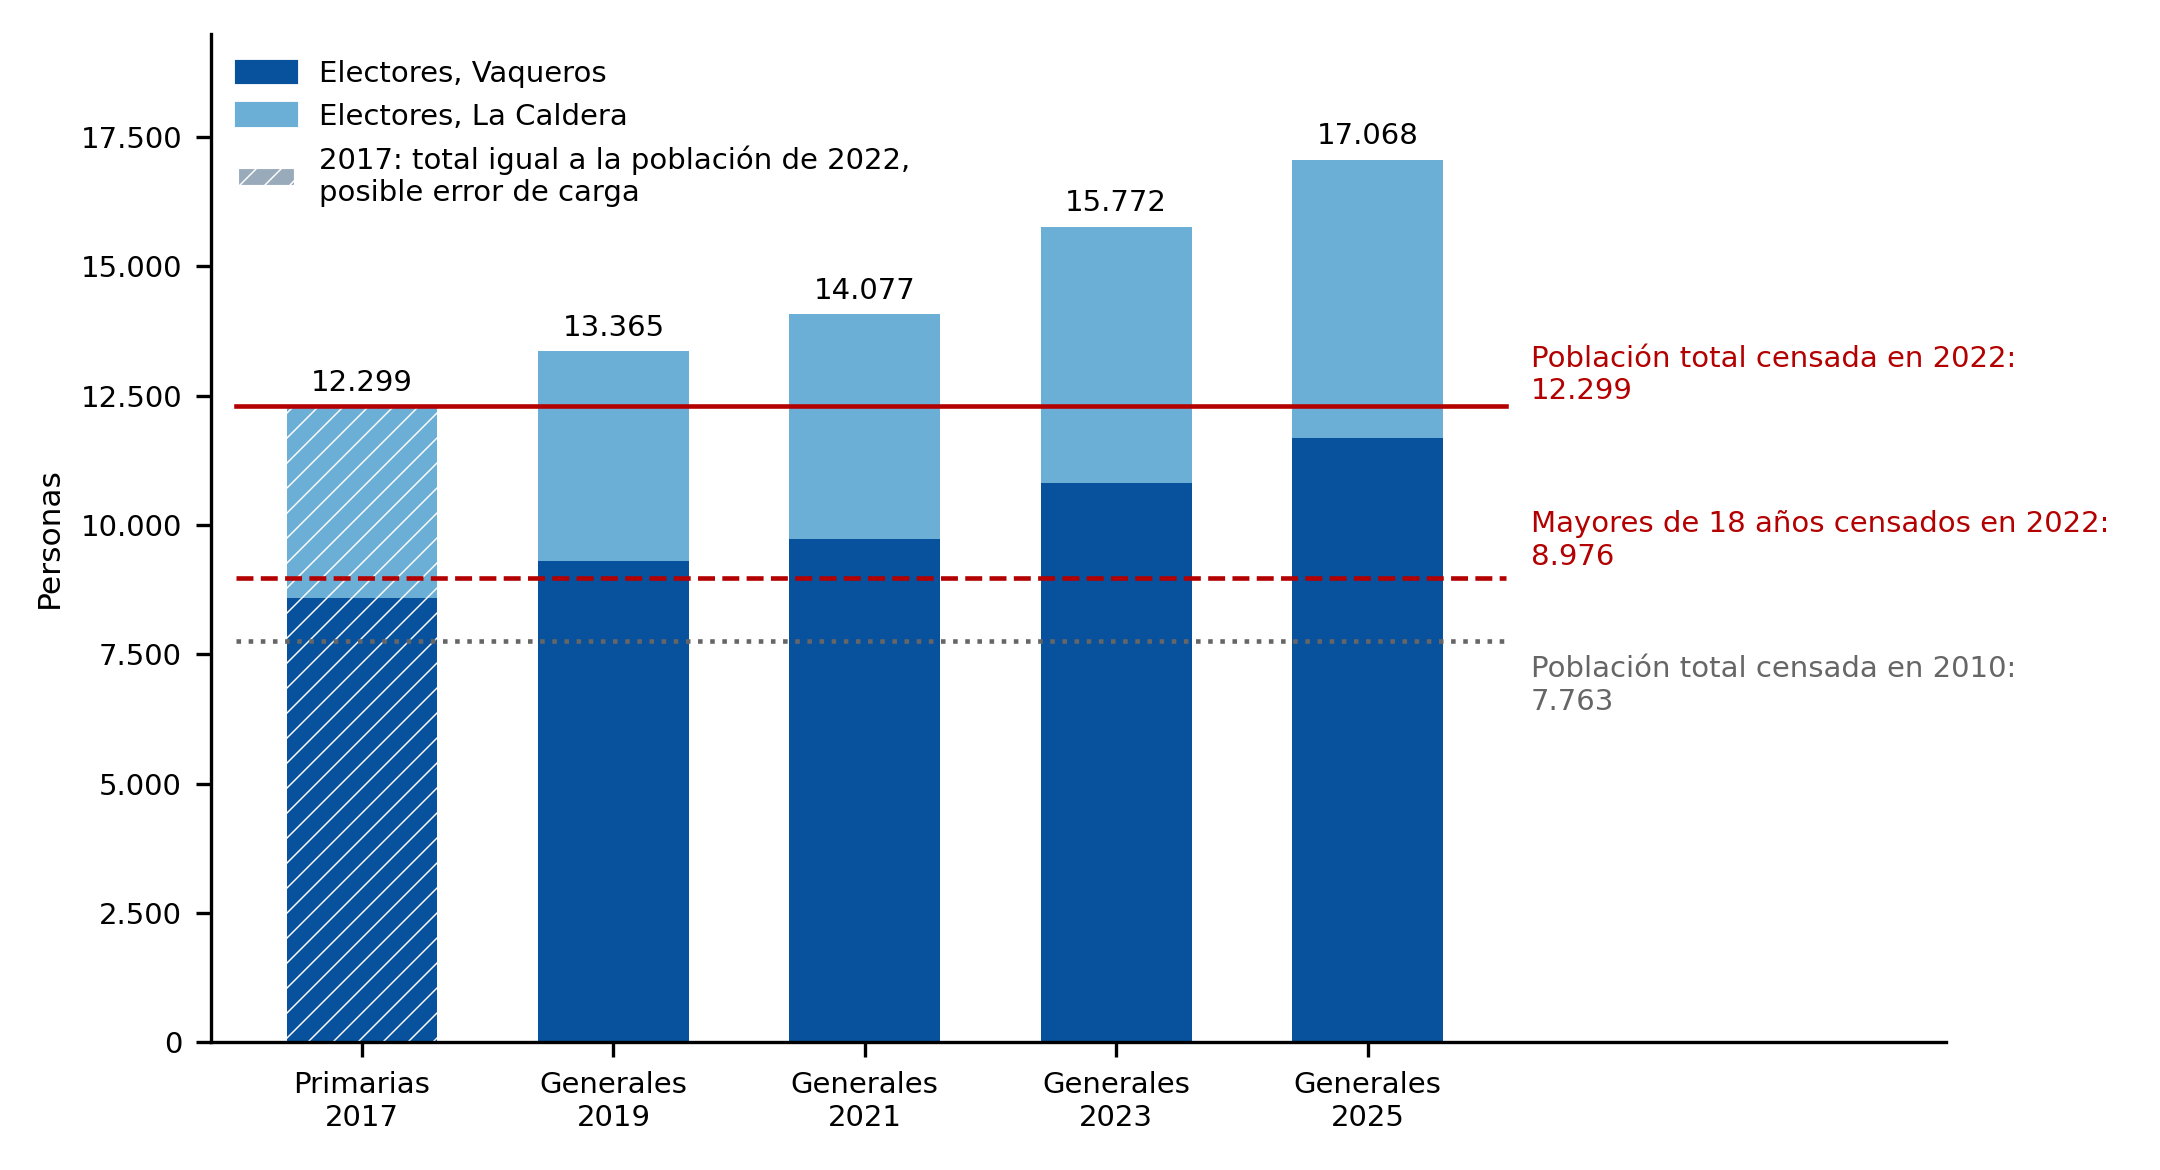
\includegraphics[width=\textwidth]{fig-padron-poblacion.png}
\caption[Padrón electoral y población del departamento, 2017--2025]{\textbf{Padrón electoral y población del departamento La Caldera, 2017--2025.} Electores habilitados por municipio en cada elección provincial, frente a la población censada en 2010 y 2022 y a los mayores de dieciocho años de 2022. La barra de 2017 va rayada: su total coincide dígito por dígito con la población de 2022 y puede ser un error de carga. Elaboración propia con datos del Tribunal Electoral de Salta y del INDEC, con \texttt{scripts/grafico\_padron.py} sobre \texttt{datos/electoral/} (repositorio \texttt{mapas\_caldera}).}\label{fig:padron}
\end{figure}

\begin{cautela}
Las cifras oficiales confirman el problema que la prensa dejaba entrever, y lo precisan. La lámina \ref{fig:padron} lo muestra en una sola imagen.

\textbf{El padrón es casi el doble de la población adulta.} El Censo 2022 registró en el departamento 12.299 habitantes, de los cuales 8.976 mayores de dieciocho años. El padrón de 2025 tiene 17.068 electores: \textbf{el 139 por ciento de toda la población censada}, niños incluidos. En la provincia, la misma relación es del 76 por ciento ---1.092.561 electores sobre 1.441.351 habitantes---, que es lo esperable en una población joven. \textbf{El departamento está más de sesenta puntos por encima de la media provincial}, y en sentido contrario al esperable.

\textbf{La diferencia es mayor en Vaqueros.} Su padrón equivale al 150 por ciento de sus 7.774 habitantes; el de La Caldera, al 119 por ciento de sus 4.525.

\textbf{Y no es reciente.} Según la planilla, en 2017 el departamento tenía 12.299 electores \textit{---cifra idéntica, dígito por dígito, a la población censal de 2022, lo que sugiere un error de carga---}, muy por encima de los 7.763 habitantes del censo de 2010. \pendiente{cotejo de la planilla de electores de 2017 contra el original del Tribunal Electoral} Si la cifra se confirma, entre 2017 y 2025 el padrón creció un 38,8 por ciento, a un ritmo del 4,2 por ciento anual, algo mayor que el 3,9 anual con que creció la población entre 2010 y 2022.

Este libro \textbf{no afirma} irregularidad alguna. La explicación más probable es legal y conocida: se vota donde figura el domicilio del documento, no donde se vive, y el Censo 2022 ---el primero \textit{de derecho} del país--- cuenta a las personas donde residen habitualmente, que para el dueño de una casa de fin de semana no es el departamento. Un departamento con casi una de cada cinco viviendas sin residentes permanentes, clubes de campo y casas de fin de semana de vecinos de la capital (capítulo \ref{cap:poblacion}) es exactamente el lugar donde cabe esperar muchos electores que no son habitantes. También puede influir que el padrón tarde en dar de baja a quienes se mudaron.

Si es así, el dato es de primer orden para este libro: \textbf{entre dos quintos y casi la mitad de quienes pueden elegir a las autoridades del departamento no vive en él} ---según se tome la población adulta de 2022 o se la proyecte a 2025, y sin descontar a quienes el padrón no dio de baja---, y es probablemente la misma población ---propietarios no residentes--- que el capítulo \ref{cap:redes} identifica entre los beneficiarios de la falta de infraestructura. Lo que falta para confirmarlo no es el tamaño del padrón, que ya se conoce, sino su composición: cuántos electores se incorporaron por cambio de domicilio y desde dónde, dato que el Tribunal Electoral no publica.
\end{cautela}




\section{1936: una mesa anulada}

Diez años antes de la convocatoria de 1946, que la sección siguiente transcribe, hay un episodio que este relevamiento no buscaba y que
conviene dejar registrado, porque cruza las dos series que el libro sigue por separado: la
electoral y la de los nombres.

\begin{ficha}{Nómina de presidentes de comicio insaculados para 1936--1937 --- Colegio Electoral Nº 2, La Caldera}
\textbf{Circuito 5, Mesa 1} (Escuela Elemental Mixta): presidente \textbf{Regis,
Augusto}\index{Regis, Augusto}; suplente 1º Robles, Eusebio José; suplente 2º \textbf{Linares,
Daniel}\index{Linares, Daniel}.

\textbf{Circuito 5, Mesa 2} (Iglesia Parroquial): presidente Alonso, Fabián; suplentes Romano,
Lorenzo, y Lozano, Juan de Dios.

\textbf{Circuito 6, Mesa 1} (Registro Civil de Vaqueros): presidente Bruzzo, Atilio José.

El encabezado del documento aclara el método: los presidentes de mesa eran
\textbf{insaculados} ---sorteados--- por el Tribunal Electoral.
\end{ficha}

Es la única pieza del archivo que pone a Augusto Regis y a Daniel Linares en la misma mesa
electoral. No es la primera que los reúne: en 1910 integraron la misma comisión de defensas, y
en 1922 un mismo decreto los designó miembros de la Comisión Municipal. El capítulo \ref{cap:fincas} los sigue por separado durante treinta años
---presidente municipal y propietario el primero, presidente de la comisión de defensas de
1910 y propietario de tres fincas el segundo---; aquí están, en 1936, como presidente y
suplente segundo de la misma mesa. \textbf{Y por sorteo}, lo que en un padrón de pocos
centenares de electores dice menos sobre la voluntad de nadie que sobre el tamaño del conjunto
del que se sorteaba.

\textbf{Esa mesa fue anulada.} Por decreto del 6 de marzo de 1936, el Ministerio de Gobierno
transcribe la comunicación del Tribunal Electoral ---firmada por David Saravia y Pedro J.\
Aranda--- que informa haber anulado la elección del domingo 1º de marzo en una lista de mesas,
entre ellas la \textbf{Mesa Nº 1 del Circuito Nº 5 de La Caldera}, y convoca a comicios
complementarios para el \textbf{domingo 15 de marzo}, por el artículo 77 de la Ley 122. Se
elegían gobernador, vicegobernador y representantes a la Legislatura.

\begin{cautela}
El decreto \textbf{no dice por qué} se anuló ninguna de las mesas de la lista: transcribe el
resultado del examen de urnas y documentación, no su fundamento. Este libro no afirma
irregularidad alguna ni la vincula con quién presidía: la anulación de mesas por vicios
formales ---documentación incompleta, actas mal labradas--- era y es corriente, y La Caldera
figura en una lista junto a mesas de otros departamentos. Lo que queda establecido es el hecho
y su fecha.
\end{cautela}

\section{Y en 1946 ya elegía uno}

Antes de llegar a 1983 conviene poner una referencia mucho más antigua, porque muestra que el
tamaño de la representación departamental no es un efecto de la reforma de 1986 ni del
crecimiento reciente.

\begin{ficha}{Decreto Nº 9686-G --- Salta, 15 de diciembre de 1945 --- Expte.\ Nº 2949/945}
Convoca al pueblo de la Provincia a elecciones nacionales y provinciales simultáneas para el
\textbf{domingo 24 de febrero de 1946}, con sujeción a los arts.\ 27, 70 y 71 de la Ley 122 de
Elecciones de la Provincia. Dictado en Acuerdo de Ministros por el Cnel.\ Ángel W.\ Escalada.

Su art.\ 4º reparte la representación legislativa en \textbf{tres escalones}:

\begin{itemize}[leftmargin=*,itemsep=1pt]
\item \textbf{La Capital}: siete diputados titulares y siete suplentes, un senador titular y uno suplente.
\item \textbf{Rosario de la Frontera, Rosario de Lerma, Metán, Anta y Orán}: dos diputados titulares y dos suplentes, un senador titular y uno suplente cada uno.
\item \textbf{Los dieciséis restantes} ---Rivadavia, La Candelaria, Iruya, Santa Victoria, \textbf{La Caldera}, Campo Santo, Chicoana, Cerrillos, La Viña, Guachipas, Cafayate, Molinos, San Carlos, Cachi, La Poma y Los Andes---: \textbf{un} diputado titular y uno suplente, \textbf{un} senador titular y uno suplente.
\end{itemize}

Publicado en diez ediciones consecutivas del 19 al 31 de diciembre de 1945 y en otras cuarenta y
cinco, del 2 de enero al 23 de febrero de 1946 (Nº 2.465 a 2.509), víspera del comicio, como manda
su propio art.\ 13º: cincuenta y cinco ediciones en total, según su marca de publicación
«e|19|12|45 -- v|23|2|46».
\end{ficha}

El comicio se hizo. Por La Caldera resultaron electos el senador \textbf{José Luis Alvarez} y el diputado \textbf{Darío Arias}, a quienes el Decreto 11198-G del 22 de abril de 1946 convoca, con los demás legisladores, a constituir las Cámaras el 26 de abril (B.O.\ Nº 2.554). La Ley 745, sancionada el 29 de agosto, fijó en esa fecha el comienzo del mandato y repartió los departamentos en dos grupos para sortear quiénes se renovaban a los dos años y quiénes a los cuatro; La Caldera ---«Caldera», sin artículo--- quedó en el primero (B.O.\ Nº 2.652). El barrido de 1946 no encontró el resultado del sorteo, que la ley manda hacer en el primer período de sesiones ordinarias.

Ochenta años después, y con el departamento cuadruplicado ---2.831 habitantes en el censo de 1947, 12.299 en el de 2022---, \textbf{la asignación es la misma}:
un diputado y un senador. Lo que cambió en el intervalo ---la reforma de 1986, la elección
directa del intendente, el crecimiento demográfico más alto de la provincia--- no tocó el
escalón en el que La Caldera está colocada dentro del reparto legislativo.

\section{Qué era La Caldera en 1983}

La búsqueda de los primeros intendentes del retorno democrático encontró otra cosa, mejor: encontró que no había intendentes. Cuatro ediciones del Boletín Oficial de 1983 permiten reconstruir qué era, institucionalmente, el municipio en el momento en que empieza el período que este libro estudia.

\subsection*{No se elegía el ejecutivo municipal}

\begin{ficha}{Ley 6131, promulgada el 30 de julio de 1983 --- B.O.\ Nº 11.780}
Convoca al pueblo de la Provincia a los comicios generales del \textbf{30 de octubre de 1983}.

\textbf{Art.\ 3º:} los departamentos de Cachi, Cafayate, Guachipas, Iruya, \textbf{La Caldera}, La Candelaria, La Poma, La Viña, Los Andes, Molinos, San Carlos y Santa Victoria eligen \textbf{un diputado titular y un suplente, y un senador titular y un suplente}. Es la representación mínima de la escala.

\textbf{Art.\ 4º:} para determinar el número de diputados ``rige el último censo nacional practicado en el año 1980''.

\textbf{Art.\ 5º:} convoca al pueblo de los municipios ``a fin de elegir \textbf{Concejales Municipales y Miembros de Comisiones Municipales}''. Enumera dos grupos: once municipios que eligen nueve concejales --- Capital, Tartagal, Orán, Metán, entre otros --- y dieciocho que eligen cinco. \textbf{Ni La Caldera ni Vaqueros figuran en ninguno de los dos.}
\end{ficha}

La convocatoria de 1983 no menciona intendentes. Convoca a elegir cuerpos deliberativos: concejales donde hay Concejo, miembros donde hay Comisión Municipal. El titular del ejecutivo municipal no estaba en la boleta.

Eso confirma lo que se desprende del artículo 22 de la Ley 1349 ---ver la advertencia del apéndice \ref{cap:normativa}--- y deja sin objeto la búsqueda de ``actas de proclamación de intendentes de 1983'': no existen porque no hubo elección de intendentes. \textbf{Y desplaza la pregunta}: lo que hay que buscar para ese período no son proclamaciones sino designaciones.

\subsection*{Era una Comisión Municipal, y tiene nombre}

El Boletín Nº 11.870 transcribe íntegra una ordenanza de La Caldera y el decreto provincial que la aprueba.

\begin{ficha}{Ordenanza Nº 047 del 30 de junio de 1983}
Establece para ese año una reducción del cuarenta por ciento en las tasas de Alumbrado y Limpieza a favor de jubilados y pensionados, con tres condiciones: ser titular de la \textbf{única} propiedad, que el inmueble sea casa habitación del beneficiario, y que el haber jubilatorio no supere el mínimo de ley.

Firman: \textbf{Arturo R.\ Fernández\index{Fernández, Arturo R.}, Presidente de la Comisión Municipal de La Caldera}, y \textbf{Esteban Mogro\index{Mogro, Esteban}, Secretario Administrativo}.

Los considerandos invocan el \textbf{Decreto provincial 877/82}, que acuerda al titular del Departamento Ejecutivo Municipal, ``a más de las funciones que le son propias, \textbf{las inherentes al Concejo Deliberante}''.

La ordenanza dispone en su artículo 4º: ``Pase a Secretaría de Estado de Municipalidades \textbf{para su aprobación}''. Y en efecto, el \textbf{Decreto 1975} del Ministerio de Gobierno, Justicia y Educación la aprueba y transcribe.
\end{ficha}

\begin{cautela}
Tres capas de tutela en un solo acto de gobierno local, y las tres importan.

\textbf{La primera: no había Concejo.} El Decreto 877/82 concentró en el titular del ejecutivo las funciones del cuerpo deliberativo. Quien sancionaba la ordenanza y quien la promulgaba eran la misma persona.

\textbf{La segunda: esa persona no era un intendente sino un Presidente de Comisión Municipal}, la figura que la Ley 1349 --- entonces vigente, derogada en 2018 --- reservaba en su artículo 33 a los municipios de tercera categoría, y cuyo titular ``será nombrado y removido por el Poder Ejecutivo''.

\textbf{La tercera: la ordenanza no valía por sí sola.} Necesitaba aprobación de la Secretaría de Estado de Municipalidades, y la obtuvo por decreto ministerial. Una rebaja de tasas para jubilados de un pueblo de mil habitantes recorrió el circuito completo hasta el Boletín Oficial de la Provincia.

\textbf{Y en 1921 la elección del departamento se anula entera.} La Junta Electoral resolvió, el 6 de septiembre, \textbf{declarar nula la elección del 7 de agosto en el distrito de la Caldera} y en otros once, «\textit{por no haberse verificado elección legal en dos tercios de las mesas}»; el decreto que convoca de nuevo es del 20 de septiembre y \textbf{se publica el 28 de octubre, diecinueve días después del segundo domingo de octubre que él mismo señalaba} (capítulo \ref{cap:siglo}). \textbf{Son dos años seguidos}: en 1920 se anuló la urna de Mojotoro y hubo complementarias; en 1921, el distrito completo. Ni la nota de la Junta ni la resolución de nulidad se publican, de modo que este libro no puede decir si la elección de octubre se hizo ni qué pasó con los dos convencionales que le correspondían al departamento en la reforma constitucional.

\textbf{Y en 1920 el instrumento que fija la representación no cierra consigo mismo.} El decreto 685 del 6 de febrero de 1920, que convoca a elegir legisladores provinciales, \textbf{nombra dos veces a Caldera con un diputado cada vez} en la misma enumeración, y enumera trece departamentos de los veintidós (capítulo \ref{cap:siglo}). Ese mismo año, tres partidos proclaman candidato a diputado por el departamento, y uno de los tres ---\textbf{Dermidio Arancibia}--- es quien dos años antes había pedido las dos concesiones mineras que el Boletín registra sobre este suelo. \textbf{Coincidencia de nombre y no identificación registral}, pero es el primer caso de esta serie en que quien pide una concesión sobre el departamento se presenta a representarlo. Y la única urna anulada del departamento ese año es la de Mojotoro, que es donde está su única plaza rentada de policía, que cambió de manos tres veces en cinco meses.

\textbf{Y la tutela no empieza en 1982.} El capítulo \ref{cap:siglo} documenta que en marzo de 1918 el departamento fue incluido, por el decreto 1.557, entre los catorce que pasaban de Comisión Municipal a \textbf{Municipalidad electiva} por tener renta superior a cinco mil pesos; y que siete semanas después el decreto 1.660 lo sacó de la lista, y sólo a él, porque su cálculo de recursos había computado como renta un saldo del ejercicio anterior. \textbf{La renta real eran \$3.387,50}, y el decreto concluye que el departamento «\textit{no está en condiciones de ser administrado por una Municipalidad electiva}». La tercera categoría de la Ley 1349 es de 1933; el criterio de renta que la funda ya operaba en 1918, y ya dejaba a este departamento del lado de abajo. \textbf{Y diez meses después el gobierno siguiente cambió el fundamento sin cambiar el resultado}: el decreto 33 del 15 de enero de 1919, que nombra la Comisión Municipal del departamento, considera que el artículo de la Ley Orgánica en que se creaban municipalidades «\textit{ha sido derogado por el art.\ 175 de la Constitución, que exije para la existencia de Municipalidades autónomas un centro urbano de cinco mil habitantes, de que carecen todos los Departamentos de Campaña}». \textbf{El umbral deja de ser de pesos y pasa a ser de personas, y la cifra es la misma: cinco mil.} Es la que la Ley 1349 recogerá catorce años después como techo de la tercera categoría, y la que el capítulo \ref{cap:poblacion} encuentra todavía operando en la clasificación estadística de 2022.

De modo que el punto de partida del período que este libro estudia no es un municipio débil: es un municipio \textbf{tutelado}, sin órgano deliberativo, con ejecutivo designado y con sus actos sujetos a aprobación provincial.
\end{cautela}

\subsection*{Y confirma lo que el capítulo \ref{cap:poblacion} sospechaba}

El capítulo \ref{cap:poblacion} estableció que la clasificación M3 de la Dirección General de Estadísticas se presenta como ``municipio de tercera categoría'', que la tercera categoría de la Ley 1349 correspondía a las Comisiones Municipales, y que desde 2018 esa ley está derogada y el régimen vigente no tiene categorías. La categoría estadística, entonces, está \textbf{congelada}: sobrevive a la ley que la sostenía.

Estos documentos fechan el congelamiento. \textbf{En 1983 la clasificación era exacta}: ambos eran Comisiones Municipales. El Boletín Nº 11.870 registra que el 9 de diciembre de 1983 --- víspera del traspaso democrático --- el Poder Ejecutivo provincial aceptó las renuncias de los \textbf{Presidentes de las Comisiones Municipales} de una larga lista que incluye a \textbf{La Caldera y a Vaqueros}, y en decretos separados las de los \textbf{Intendentes de las Municipalidades}. Las dos figuras coexistían y el departamento estaba, entero, del lado de las Comisiones.

Con lo cual la categoría que hoy comparten con San Lorenzo --- treinta y dos mil habitantes --- no es un error de clasificación: es una clasificación de 1931 que en 1983 todavía era exacta, que nadie actualizó mientras la ley la exigía y que la estadística siguió usando después de derogada. Vaqueros tiene hoy 7.774 habitantes y sigue clasificado como lo estaba cuando tenía menos de dos mil: la Ley 4365 lo creó en 1970 como «municipio de tercera categoría (2da.\ clase)» (capítulo \ref{cap:cot}).

\begin{cautela}
Un dato menor que conviene registrar sin conclusión. El Boletín Nº 11.868 consigna que en noviembre de 1983 el Poder Ejecutivo aceptó la renuncia del señor \textbf{Esteban Mogro\index{Mogro, Esteban}} al cargo de \textbf{Juez de Paz Titular de la localidad de La Caldera}. Es el mismo nombre que cinco meses antes firmaba la Ordenanza 047 como Secretario Administrativo de la Comisión Municipal.

Puede tratarse de dos cargos sucesivos o simultáneos, y de la misma persona o de dos homónimos en una localidad de mil habitantes. Este libro no lo establece. Lo consigna porque, si se confirma la simultaneidad, describe algo característico de las localidades pequeñas: la administración municipal y la justicia de paz atendidas por la misma mano.
\end{cautela}


\section{Lo que la banca dejó atrás}

El traslado de Moreno al Senado tuvo una consecuencia que este libro debe registrar, porque no ocurre en la Legislatura sino en el municipio donde se concentra la conversión de suelo del departamento.

Moreno renunció a la intendencia de Vaqueros faltando dos años de mandato. La regla aplicable no es la vieja Ley Orgánica de Municipalidades, derogada en 2018, sino el Régimen de Municipalidades de la \textbf{Ley 8126} (B.O.\ 17/12/2018). Su artículo 64 pone el Ejecutivo, en caso de impedimento, a cargo del presidente del Concejo Deliberante, cargo que el propio cuerpo elige cada año (art.\ 50); y su artículo 67 dispone que, si la renuncia es definitiva y falta \textbf{más de un año} para completar el mandato, \textbf{debe convocarse a elecciones} conforme el artículo 182 de la Constitución provincial. Faltaban dos. \pendiente{convocatoria a elecciones para completar el mandato de intendente de Vaqueros conforme el art.\ 67 de la Ley 8126, o acto que la descarte}

\begin{ficha}{Tres titulares del Ejecutivo en tres meses}
\begin{itemize}[leftmargin=*,nosep]
\item \textbf{Diciembre de 2025.} Moreno renuncia. Asume el Ejecutivo \textbf{Daniel Viveros}, concejal y entonces presidente del Concejo Deliberante.
\item \textbf{1 de marzo de 2026.} En la primera sesión del año, el Concejo elige presidenta a \textbf{Andrea Salvatierra}, lo que conforme a la normativa vigente en el municipio la habilita a asumir la intendencia interina. Viveros sostiene que no corresponde desplazarlo, porque la renuncia de Moreno fue definitiva y su asunción debe extenderse hasta una nueva convocatoria a elecciones.
\item \textbf{Primeros días de marzo de 2026.} Viveros recurre a la Justicia, denuncia un ``golpe institucional'' y solicita medida cautelar de no innovar. La \textbf{Corte de Justicia de Salta} rechaza el planteo: la elección de autoridades del Concejo es facultad legítima del cuerpo y no se acreditó irregularidad en el procedimiento. Salvatierra, que había jurado el 2 de marzo, queda confirmada; el fallo es del 3 de marzo.
\item \textbf{Mayo de 2026.} El senador Moreno ratifica públicamente su respaldo a la gestión de Salvatierra y marca distancia de la etapa anterior.
\end{itemize}
\textit{Fuente: cobertura de prensa provincial, diciembre de 2025 a mayo de 2026. Los textos de la resolución del Concejo y del fallo de la Corte no fueron consultados.}
\end{ficha}

\begin{cautela}
Lo que este episodio agrega no es color político. Es un dato de capacidad estatal, y es del mismo orden que los que el capítulo \ref{cap:redes} reúne.

Entre diciembre de 2025 y marzo de 2026, el municipio más presionado del departamento --- el que aprueba fraccionamientos, otorga factibilidades, emite certificados de aptitud ambiental y ejerce el poder de policía sobre la obra privada --- tuvo \textbf{tres titulares del Ejecutivo en tres meses}, y el tercero llegó tras una disputa que debió resolver la Corte provincial. La Ley 8126 sólo prevé la intervención de la Corte para el juicio político al intendente (art.\ 92); la vía por la que llegó este conflicto es la que la prensa describe, una cautelar de no innovar, y el fallo no se consultó.

Ese es también el período de la última reforma del Código de Planeamiento Urbano Ambiental de Vaqueros: la Ordenanza 648/26, promulgada por el Decreto 486/26 del \textbf{26 de enero de 2026}, que firma «J.\ Daniel Viveros, Intendente». La reforma que incorporó los distritos de la costanera se promulgó, entonces, durante el interinato que el Concejo daría por terminado cinco semanas después. El capítulo \ref{cap:vaqueros} analiza el texto que resultó de ella.

Corresponde una advertencia expresa, porque el material se presta a la insinuación y este libro no la hace: \textbf{no se encontró vinculación documental alguna entre la disputa por la presidencia del Concejo y materia urbanística}. Lo que se registra es la discontinuidad del Ejecutivo municipal en un trimestre determinado, no una hipótesis sobre su causa.
\end{cautela}


\section{El voto que impide la tesis fácil}

En diciembre de 2024, la actualización del Ordenamiento Territorial de Bosques Nativos fue aprobada por el Senado provincial con amplia mayoría y tres votos en contra: los senadores por Cachi, por San Martín y \textbf{por La Caldera}. Esa norma es la \textbf{Ley provincial Nº 8483}, publicada en el Boletín Oficial el 3 de enero de 2025, que revisa el ordenamiento, modifica las superficies por categoría de conservación e introduce la figura del Área de Producción y Conservación. Su contenido se analiza en el capítulo \ref{cap:opacidad}. El senador por La Caldera es, además, el impulsor de la prórroga de la ley provincial de suspensión de desalojos de familias rurales hasta diciembre de 2026, norma que \textit{El dispositivo salteño} consignó en su apéndice sobre litigio territorial.

El registro nominal de esa votación es el contrapeso más fuerte que este libro tiene contra su propia tesis, y por eso va en el cuerpo del capítulo y no escondido en una nota. La representación departamental en la cámara que aprueba el mapa de bosques votó contra ese mapa.

De aquí se sigue una redirección del objeto. Si la banca senatorial no es el punto de captura, entonces la decisión efectiva sobre el uso del suelo ocurre donde este libro la encontró: la ordenanza del Concejo Deliberante, el certificado de aptitud ambiental municipal y el expediente de la Secretaría de Ambiente provincial. Tres instancias técnicas, de baja visibilidad pública, sin votación nominal publicada y sin cobertura periodística sistemática.

Ese desplazamiento --- del órgano político visible al órgano técnico opaco --- se desarrolla en el capítulo \ref{cap:opacidad}, que es donde este libro reúne el conjunto de la evidencia sobre el punto.

\section{El proyecto de reserva, y la tensión que abre}

En marzo de 2023, siendo senador, Calabró presentó ante la Cámara un proyecto para crear un área protegida sobre la Ruta Nacional 9, en el norte del departamento.

\begin{ficha}{Expte.\ Nº 90-31.780/2023 --- Reserva Natural Corredor Biológico Abra de Santa Laura}
Presentado el \textbf{30 de marzo de 2023} por el senador \textbf{Héctor Miguel Calabró\index{Calabró, Héctor Miguel}}, girado a la \textbf{Comisión de Minería, Recursos Naturales y Medio Ambiente}.

\textbf{Art.\ 1º:} instituye la Reserva Natural Corredor Biológico Abra de Santa Laura en el departamento La Caldera, ``de acuerdo al contenido de la \textbf{Ley Provincial 4.736}''.

\textbf{Art.\ 3º --- fijación de límites:} ``se efectuará sobre el eje del \textbf{talweg del río Porongal}, y su área de influencia de media y alta Sub Cuenca'', conforme los estudios y mensuras que establezca el Poder Ejecutivo por decreto, que además debe designar autoridad de aplicación entre los Ministerios de Producción, Ambiente y Turismo. Dentro de los noventa días de aprobado, debe elaborarse la reglamentación de funcionamiento.

\textbf{Art.\ 4º:} invita a asesorar a la Universidad Nacional de Salta --- Facultades de Ciencias Naturales y de Economía --- y a la Universidad Católica de Salta, Escuela de Turismo.

\textbf{Art.\ 5º --- Dominio Público:} ``Se declaran de Dominio Público Provincial las tierras comprendidas en este Corredor Biológico, conforme el régimen jurídico sustentado en \textbf{acuerdos con los propietarios} de las mismas, \textbf{sin necesidad de expropiaciones}'', por analogía con la Ley 6.806/95 de la Reserva Natural de la Quebrada de las Conchas.

\textbf{Destino: caducó.} Consta en el registro de proyectos caducados de la Cámara, por aplicación de la Ley 1111, con fecha \textbf{13 de marzo de 2025}. Nunca fue tratado.
\end{ficha}

\begin{cautela}
Cinco observaciones sobre el texto, en orden de importancia.

\textbf{Primera: caducó.} El proyecto entró en marzo de 2023, fue girado a comisión y ahí quedó. La Ley 1111 lo dio por caduco en marzo de 2025, nueve meses antes de que terminara el mandato de su autor. La reserva no existe y nunca estuvo cerca de existir.

\textbf{Segunda: no invoca la ley vigente.} El artículo 1º remite a la Ley provincial 4.736, no a la Ley 7107 del Sistema Provincial de Áreas Protegidas, sancionada en 2000 y vigente. Este libro \textbf{no afirma que la 4.736 esté derogada}: el texto completo de la Ley 7107, obtenido y leído, \textbf{no contiene artículo derogatorio alguno} --- su artículo 63 se limita a remitir supletoriamente a la Ley 7070, y su artículo 35 inciso c faculta a ``recategorizar si correspondiere, las áreas protegidas existentes en la Provincia al momento de la promulgación''. Si la 4.736 subsiste, en qué medida y con qué alcance, es una cuestión que excede a este trabajo.

Lo comprobable es que el proyecto se apoyó en una norma anterior al régimen integral vigente, y no en el régimen integral vigente --- que es, además, el que el capítulo \ref{cap:tierra} identificó como el instrumento disponible y no usado en el departamento.

\textbf{Tercera: la ley no era la única vía, ni la más rápida.} Los artículos 60 y 61 de la Ley 7107 permiten declarar un área protegida por \textbf{acto administrativo del Poder Ejecutivo}, de oficio o a petición de parte, previa evaluación de la Autoridad de Aplicación. Un proyecto de ley que caduca en comisión no agota el asunto: la vía administrativa quedaba abierta antes, durante y después. Y una vez declarada por decreto, el área sólo puede alterarse por ley --- artículo 62 ---, de modo que esa vía produce además un resultado más difícil de revertir.

\textbf{Cuarta: el artículo 5º del proyecto es jurídicamente singular.} Declara de dominio público provincial tierras privadas ``conforme acuerdos con los propietarios'' y ``sin necesidad de expropiaciones''. El dominio público no se constituye por acuerdo. El artículo 51 de la Ley 7107 prevé lo contrario: obliga a impulsar expropiación cuando las restricciones impidan el ejercicio regular de los derechos. Y su artículo 53 ofrece la figura que el proyecto parecía buscar sin nombrarla --- la incorporación voluntaria del propietario, con beneficios impositivos y renuncia no admisible antes de veinte años ---, que no requiere declarar público lo privado.

\textbf{Quinta: la geografía del texto no coincide con la de la prensa.} La cobertura de julio de 2023 ubicó la reserva entre los kilómetros 1.642 y 1.650 de la Ruta 9, del Dique Campo Alegre al límite con Jujuy. El articulado la ubica sobre el eje del \textbf{talweg del río Porongal} y su subcuenca media y alta. Pueden ser la misma zona descripta de dos maneras --- una por la ruta, otra por la cuenca ---, y este libro no afirma que no lo sean. Cabe consignar que el instrumento delimita por hidrografía y la difusión por kilometraje vial.
\end{cautela}

\begin{cautela}
Un nombre que conviene retener sin sacar conclusiones. La Ley 4486 --- analizada en el capítulo \ref{cap:expropiacion} --- expropió en 1972 una fracción de la finca \textbf{Los Porongos}, que el artículo 6º del PDUA sigue enumerando entre las unidades del municipio. El proyecto de reserva delimita por el \textbf{río Porongal}. La proximidad toponímica es evidente y puede no significar nada: los topónimos se repiten sobre cuencas y las fincas suelen llevar el nombre del curso que las atraviesa.

Establecer si hay relación --- y de haberla, cuál --- requiere el antecedente dominial de esa finca y la cartografía de la subcuenca. Es una de las cuatro o cinco preguntas que este libro deja abiertas sobre el mismo hueco: quién es dueño de qué en el departamento.
\end{cautela}

\begin{cautela}
Corresponde ahora enunciar, con la mayor precisión posible, una tensión que este libro documenta y no resuelve.

El capítulo \ref{cap:loteo} establece, con avisos del Boletín Oficial, que \textbf{Héctor Miguel Calabró\index{Calabró, Héctor Miguel} ---identificado por el mismo número de documento que en el acta de proclamación de 2011--- fue designado gerente suplente de Jardín Celestial S.R.L.} por acta del 8 de noviembre de 2018, publicada en enero de 2020, sin que este relevamiento haya encontrado constancia posterior de su cese ni de su continuidad; y que esa sociedad es copropietaria del inmueble sobre el que se aprobó el plano del loteo El Durazno, en el sur del pueblo de La Caldera. Este capítulo establece que, en marzo de 2023, el mismo Calabró impulsó como senador un área protegida para frenar el avance inmobiliario, en el norte del departamento.

\textbf{Las dos cosas no se contradicen en el plano de los hechos.} La reserva propuesta y el loteo están en extremos opuestos del departamento, separados por el pueblo y por el embalse; proteger un tramo de Yungas sobre la cornisa no impide nada en la zona sur. Un legislador puede impulsar conservación en un lugar y tener interés societario en otro sin incurrir en irregularidad alguna, y este libro no afirma que la haya.

Lo que efectivamente queda registrado, y es un dato estructural, es que \textbf{la misma persona fue designada en 2018 en el órgano de administración de una sociedad desarrolladora del departamento ---designación publicada en 2020, sin constancia posterior de cese--- y ocupó entre 2021 y 2025 la banca que legisla sobre el uso del suelo de ese departamento}, y que desde esa banca votó en diciembre de 2024 contra la Ley 8483 e impulsó en 2023 un área protegida.

Este libro no atribuye intención a ninguno de esos actos. Enuncia la superposición de posiciones porque es verificable en instrumentos públicos, y porque la superposición de posiciones --- no la mala fe --- es exactamente el objeto que ambos libros describen. La verificación que falta, y que es previa a cualquier publicación, es el derecho a réplica: si seguía siendo gerente suplente durante su mandato de senador y, en ese caso, qué dice el propio Calabró sobre la compatibilidad entre ambas posiciones, si informó la participación societaria en las declaraciones juradas patrimoniales que la normativa exige a los legisladores, y si se excusó en alguna votación relativa al departamento.
\end{cautela}


\section{La heterogeneidad del poder local}

El libro documentó, sobre el mismo cuerpo deliberativo y en la misma semana de enero de 2026, dos actos de signo opuesto: el pedido de clausura preventiva del ingreso a un loteo cerrado y la promulgación de una ordenanza, sancionada a fines de 2025, que prohíbe cobrar el acceso al perilago de un embalse público. Documentó también que el propio municipio denunció y logró la clausura de un loteo ilegal en 2020, y que su Concejo pidió la clausura de dos campings en 2026.

La descripción del dispositivo caldereño debe incluir su heterogeneidad o no describe nada. No hay aquí un poder local capturado enfrentado a una sociedad civil indefensa: hay un aparato que denuncia y habilita, que clausura y agradece la inversión, y cuyas fisuras internas son tan documentables como sus continuidades.

Lo que este libro sostiene no es que alguien haya capturado al Estado local. Es que se le asignó una función sin los medios para ejercerla, y que el resultado de esa asimetría se distribuye de manera muy desigual entre quienes habitan el territorio.

\begin{cautela}
Sobre la serie de intendencias, este relevamiento avanzó de manera desigual y conviene separar los tramos por su grado de verificación.

\textbf{Verificado en fuente oficial.} Se obtuvieron las actas de proclamación de electos del Tribunal Electoral de la Provincia correspondientes a las elecciones generales del \textbf{10 de abril de 2011} y del \textbf{17 de mayo de 2015}. Ambas consignan, para el departamento La Caldera:

\begin{center}\small
\begin{tabular}{@{}lll@{}}
\toprule
\textbf{Año} & \textbf{Cargo} & \textbf{Electo} \\
\midrule
2011 & Diputado & Héctor Miguel Calabró\index{Calabró, Héctor Miguel} (PJ) \\
2011 & Intendente de La Caldera & \textbf{Luis Gerardo Mendaña\index{Mendaña, Luis Gerardo}} (PJ) \\
2011 & Intendente de Vaqueros & Daniel Roberto Moreno Ovalle\index{Moreno Ovalle, Daniel Roberto} (SST) \\
2015 & Intendente de La Caldera & \textbf{Daniel Alejandro Escalera\index{Escalera, Daniel Alejandro}} (PJ) \\
2015 & Intendente de Vaqueros & Daniel Roberto Moreno Ovalle\index{Moreno Ovalle, Daniel Roberto} (PV) \\
\bottomrule
\end{tabular}
\end{center}

\textbf{La contradicción quedó resuelta.} Un listado de segunda mano atribuía la intendencia electa en 2011 a ``Luis Gerardo Escalera''. El acta oficial dice \textbf{Luis Gerardo Mendaña\index{Mendaña, Luis Gerardo}}. El error del listado consistía en unir el nombre de pila de uno con el apellido del otro --- Escalera es el electo en 2015, no en 2011 ---, y es un buen recordatorio de por qué este libro no publica lo que no verifica.

Del tramo anterior, \textbf{Héctor Miguel Calabró\index{Calabró, Héctor Miguel} fue intendente entre 1999 y 2011}, en tres mandatos consecutivos, sucediendo a \textbf{Horacio Martín Quipildor}. Eso no consta en actas obtenidas sino en tres fuentes periodísticas coincidentes, incluida una nota de Página/12 de 2021 donde el propio Calabró declara que en 2010 ``era intendente''. Varios decretos provinciales lo confirman para el tramo final ---el 1639/07, el 4354/09 y el 556/10 aprueban convenios que firma como intendente---, entre ellos dos que lo nombran expresamente en ese carácter: el Decreto 3318/08 (B.O.\ Nº 17.931, 19/08/2008) lo designa presidente de la Comisión Directiva de la Cooperadora Asistencial de La Caldera en su carácter de «Intendente Municipal», y el Decreto 2508/09 (B.O.\ Nº 18.129, 18/06/2009), que aprueba un convenio con el PAMI para la refacción y ampliación del Hogar de Ancianos del pueblo, lo nombra en el Comité Coordinador como «Intendente Municipal de la localidad de La Caldera». El inicio del mandato en 1999 y las dos reelecciones siguen apoyados en la prensa.

\textbf{No corroborado, y por lo tanto no publicable.} Ese mismo listado propone para 1983, 1987 y 1991 tres nombres --- Roberto Adán Galli, Alberto Javier Alderete y Víctor Abelardo Montoya --- que ninguna fuente independiente respalda. \textbf{Quedan fuera del libro} hasta que aparezcan en las proclamaciones del Tribunal Electoral, que es donde constan.
\end{cautela}

\begin{ficha}{Intendencias de La Caldera --- lo verificado}
\begin{center}\small
\begin{tabular}{@{}llp{4.2cm}@{}}
\toprule
\textbf{Período} & \textbf{Titular} & \textbf{Estado} \\
\midrule
1983--1999 & --- & Sin verificar \\
hasta 1999 & Horacio Martín Quipildor & Prensa coincidente \\
1999--2011 & Héctor Miguel Calabró\index{Calabró, Héctor Miguel} & Prensa coincidente (tres mandatos); \textbf{Boletín Oficial} para 2007 a 2010 \\
2011--2015 & Luis Gerardo Mendaña\index{Mendaña, Luis Gerardo} & \textbf{Acta de proclamación} \\
2015--2019 & Daniel Alejandro Escalera\index{Escalera, Daniel Alejandro} & \textbf{Acta de proclamación} \\
2019--2027 & Diego Ramiro Sumbay\index{Sumbay, Diego Ramiro} & Prensa coincidente; actas no obtenidas \\
\bottomrule
\end{tabular}
\end{center}
\end{ficha}

\begin{cautela}
La serie verificada obliga a registrar una coincidencia temporal, y este libro la enuncia con el mismo cuidado con que enunció las anteriores.

Jardín Celestial S.R.L.\ se constituyó por instrumento publicado en el Boletín Oficial del \textbf{1 de diciembre de 2010}. El capítulo \ref{cap:loteo} documenta que entre sus socios fundadores figura \textbf{Carlos Miguel Calabró\index{Calabró, Carlos Miguel}}, entonces de diecinueve años y estudiante, con el treinta por ciento del capital. En esa fecha, \textbf{Héctor Miguel Calabró\index{Calabró, Héctor Miguel} era intendente de La Caldera} y lo sería hasta diciembre de 2011.

Es decir: la sociedad que años después sería copropietaria del inmueble del loteo El Durazno se constituyó, con un socio de ese apellido, durante el tercer mandato del intendente del municipio donde la sociedad tenía su objeto.

\textbf{Este libro no sostiene que exista relación entre ambos hechos.}

Sobre el parentesco, este libro se atiene a lo que puede acreditar. El vínculo entre Héctor Miguel Calabró\index{Calabró, Héctor Miguel} y Carlos Miguel Calabró\index{Calabró, Carlos Miguel} es \textbf{altamente probable} --- apellido y segundo nombre compartidos, ambos domiciliados en La Caldera en 2010, diferencia de edad compatible --- pero \textbf{no está acreditado con partida del Registro Civil}, y por eso ni este capítulo ni el \ref{cap:loteo} lo afirman. Se acredita con una partida, no con un apellido, y es una de las preguntas del pedido de derecho a réplica. Tampoco afirma que la constitución de una sociedad de cementerio parque durante una intendencia tenga nada de irregular, porque no lo tiene.

Lo que corresponde registrar es la secuencia, porque es verificable y porque el libro registró todas las demás: 2010, constitución con un socio de ese apellido, bajo esa intendencia. 2014, ampliación del objeto social a la comercialización y adquisición de inmuebles. 2018, designación de Héctor Miguel Calabró\index{Calabró, Héctor Miguel} como gerente suplente. 2021, aprobación del plano del loteo. Cada uno de esos actos es público y ninguno, por sí mismo, es objetable.

El vínculo familiar, si existe, se acredita con partidas del Registro Civil, y es uno de los puntos que el pedido de derecho a réplica debe plantear de manera directa antes de que este pasaje se publique.
\end{cautela}

\subsection*{Dos hallazgos laterales de las actas}

Las actas de proclamación son documentos exhaustivos --- consignan cada cargo de cada municipio de la provincia con nombre y documento --- y de ellas se desprenden dos datos que este libro no buscaba.

\begin{cautela}
\textbf{El primero es un apellido a caballo del límite.} El acta de 2015 registra, para el municipio de Vaqueros, al intendente \textbf{Daniel Roberto Moreno Ovalle\index{Moreno Ovalle, Daniel Roberto}}. Y registra, para el municipio de \textbf{Salta capital}, al concejal \textbf{Mario Enrique Moreno Ovalle}, electo por la misma fuerza --- Partido de la Victoria --- en la misma elección.

Los números de documento de ambos, que el acta consigna y este libro no reproduce, son \textbf{consecutivos}. No se afirma parentesco, que se acredita con partidas y no con numeración, pero deja constancia de que dos personas de igual apellido compuesto y documento de numeración correlativa ocuparon simultáneamente, en 2015, un cargo ejecutivo en Vaqueros y uno deliberativo en la capital.

Y eso importa por lo que el capítulo \ref{cap:vaqueros} estableció: el río Vaqueros es el \textbf{límite} entre ambas jurisdicciones, y ninguna de las dos tiene competencia sobre el conjunto del cauce. Que un mismo apellido ocupara posiciones en las dos orillas en el mismo período es un dato de estructura política, no una imputación, y merece verificarse antes que interpretarse.
\end{cautela}

\textbf{El segundo es un apellido antes de tiempo.} Entre los concejales electos de La Caldera en 2015 figura \textbf{Alfio Edgardo Sumbay}, por el Frente Renovador. Cuatro años después, Diego Ramiro Sumbay\index{Sumbay, Diego Ramiro} ganaría la intendencia por una fuerza distinta, el Movimiento Comunitario Pluricultural.

De nuevo: mismo apellido, sin parentesco acreditado. Lo que la observación aporta al capítulo es que el apellido que hoy conduce el municipio ya tenía representación en el Concejo cuatro años antes, y por otra fuerza política. La política departamental no se lee sólo por partidos.

Un tercer dato, menor pero útil para el capítulo \ref{cap:poblacion}. En 2011 y en 2015, tanto La Caldera como Vaqueros eligieron \textbf{tres concejales} por acta. Si el Concejo tenía cinco miembros, como los de segunda categoría de la Ley 1349 entonces vigente, eso indicaría renovación parcial del cuerpo; las actas no dicen cuántos lo integraban. Y Moreno Ovalle\index{Moreno Ovalle, Daniel Roberto} fue electo intendente de Vaqueros en 2011 por Salta Somos Todos y en 2015 por el Partido de la Victoria: dos sellos distintos en dos elecciones consecutivas, antes de los que usaría en 2019 y 2023.

\textbf{De dónde venía el error.} El listado no corroborado proponía para 1983 a \textbf{Roberto Adán Galli}. Ese nombre existe y corresponde a un intendente real, pero de otra jurisdicción: Galli fue el \textbf{primer intendente de la Ciudad de Salta} tras el retorno democrático, sucediendo al interventor Néstor Salvador Quintana el 10 de diciembre de 1983 (artículo «Néstor Salvador Quintana» de Wikipedia en español, fuente terciaria, consultado el 18 de septiembre de 2026; y la necrológica de Galli en \textit{Iruya.com}, 26 de mayo de 2013, \url{http://noticias.iruya.com/newnex/sociedad/gente/7774-ha-fallecido-en-salta-el-ingeniero-roberto-adan-galli.html}). Y no es el único: \textbf{Alberto Javier Alderete}, que el mismo listado proponía para 1987, fue según \textit{La Gaceta Salta} (16 de mayo de 2015) el primer intendente de la capital elegido por voto directo. El listado había tomado la serie de la capital y la había atribuido al departamento, del mismo modo que había fundido a Mendaña\index{Mendaña, Luis Gerardo} con Escalera\index{Escalera, Daniel Alejandro}.

Se consigna porque ilustra el riesgo con precisión: un resumen de segunda mano no inventa de la nada, mezcla series contiguas. Y el resultado tiene la apariencia exacta de un dato.

\begin{cautela}
\textbf{Y hay una razón por la que ese tramo puede no existir como se lo está buscando.}

Galli, según esas dos fuentes ---ninguna de ellas un acto administrativo: el decreto de designación sigue sin obtenerse---, no fue electo sino \textbf{designado por el gobernador} Roberto Romero. Eso es coherente con el artículo 22 de la Ley 1349 --- el que el apéndice \ref{cap:normativa} señala como fósil administrativo ---, según el cual los intendentes ``serán nombrados y removidos por el P.E.\ con acuerdo del Senado''. Ese régimen rigió hasta que la Constitución provincial de 1986 introdujo la elección directa.

De donde se sigue que, entre 1983 y 1987, \textbf{es probable que no existan actas de proclamación de intendentes electos}, porque los intendentes no se elegían: se designaban. Buscarlas en el Tribunal Electoral sería buscar en el lugar equivocado. Lo que habría para ese período son \textbf{decretos de designación} del Poder Ejecutivo provincial, con acuerdo del Senado, publicados en el Boletín Oficial.

Para La Caldera y Vaqueros, que eran Comisiones Municipales (véase más arriba), lo que habría son decretos de designación de \textit{presidentes de comisión}, que el artículo 33 dejaba en manos del Poder Ejecutivo sin acuerdo del Senado; el acuerdo regía para los intendentes de primera y segunda categoría, como el de la capital. No se afirma aquí cómo ocurrió en La Caldera --- no lo verificó ---, pero corrige la instrucción: para 1983--1987 hay que buscar decretos, no proclamaciones.
\end{cautela}



\chapter{Las resistencias y sus límites}

\label{cap:resistencias}
Un libro que sigue expedientes corre el riesgo de describir un territorio donde sólo hay
Estado y mercado. Este capítulo mira lo demás: quiénes reclamaron, qué consiguieron, qué
no, y quiénes no aparecen en ninguna de las fuentes que este trabajo pudo leer. Incluye
además las dos actividades que ocupan el suelo del departamento sin ser ni loteo ni
agricultura —la extracción de áridos y la minería—, porque son las que mejor muestran
sobre qué se monta todo lo anterior.

\section{Las comunidades existen, y el Estado lo certificó}

Este libro declaró, entre sus límites, que no pudo verificar la existencia de comunidades
originarias en el departamento ni la de consulta previa. \textbf{Las dos cosas existen, están
certificadas por organismos del Estado y constan en el expediente del amparo.} Corresponde
corregirlo de frente y en el lugar donde más pesa.

\begin{ficha}{Expediente Nº 0010007-67527/2019-28 --- Fiscalía de Estado de la Provincia de Salta}
El 3 de agosto de 2023, la \textbf{Dra.\ Paula Herrando} solicita los antecedentes
territoriales «a fin de convocar a las comunidades originarias a los talleres participativos
para la elaboración e implementación del \textbf{Plan Integral de Manejo de la Microcuenca del
Río La Caldera}». Eleva el pedido el Coordinador General de Fiscalía de Estado,
Dr.\ Pablo G.\ Buccianti, al Subsecretario de Regularización Territorial y Registro de
Comunidades Indígenas, Dr.\ Ariel Sánchez, el 7 de agosto. El alcance 28 del expediente ---abierto en 2019--- se inicia en la mesa de
entradas de Fiscalía el 9, con carátula de pedido «en carácter urgente», y la Secretaría lo
devuelve con los dos informes el 10: \textbf{un día de trámite}.

\textbf{Informe de la Dirección de Registro de Comunidades Indígenas (10 de agosto de 2023).}
El Dr.\ Sebastián Ramiro González ratifica la presencia en el departamento La Caldera de:
\textbf{Comunidad Originaria Kolla Kondorwaira}, con personería reconocida por Resolución
Ministerial Nº 280/2009, en \textbf{Potrero de Castilla --- Vaqueros}; y \textbf{Comunidad
Indígena Kolla Urkuwasi}, con trámite de personería en el expediente 54-142017/2018-0. \textit{La invitación a la consulta que la Subsecretaría le cursa el 6 de septiembre le asigna otro número de personería: «Expte.\ Nº 224-252732/18». El libro no puede decir cuál es el correcto.}

\textbf{Informe del Equipo Técnico de la Ley 26.160 (misma fecha).} La Ing.\ Rosana Serapio
certifica que \textbf{la zona alta de la cuenca del río La Caldera es territorio de ocupación
actual, tradicional y pública de la Comunidad Originaria Kolla Kondorwaira}, según el
relevamiento centralizado del INAI de 2011, aprobado por Resolución INAI Nº 617/2013.
\end{ficha}

Cinco cosas.

\textbf{Primera: hay dos comunidades, y una tiene personería desde 2009.} No es una presunción
ni una reivindicación en disputa: es un registro estatal con número de resolución. La segunda
tiene expediente de personería en trámite desde 2018.

\textbf{Segunda: el territorio está relevado desde 2011 y aprobado desde 2013.} La Ley 26.160
ordenó relevar la ocupación tradicional de las comunidades; el relevamiento se hizo, se
centralizó en el INAI y se aprobó por resolución. \textbf{Ese relevamiento existe desde antes
de que se aprobara ninguno de los loteos que este libro documenta.}

\textbf{Tercera: la comunidad Kondorwaira está en Potrero de Castilla.} El capítulo \ref{cap:fincas} documenta
que «Potrero de Castilla» es uno de los trece partidos policiales en que la provincia dividió
el departamento en 1909, y que el artículo 6º del plan urbano de 2015 lo sigue enumerando
entre las unidades del municipio. \textbf{La unidad administrativa más antigua del archivo y el territorio comunitario reconocido por el INAI llevan el mismo nombre.} Y el río Potrero de Castilla es, por la Ley 4987, el tramo alto del límite entre La Caldera y Vaqueros (capítulo \ref{cap:cot}): eso explica que el registro sitúe a la comunidad en «Potrero de Castilla --- Vaqueros» mientras el plan urbano de La Caldera enumera ese paraje como propio. El paraje está sobre la línea que separa a los dos municipios.

\textbf{Cuarta, y es lo que más importa: la zona alta de la cuenca es territorio de ocupación
tradicional.} La zona alta es la cabecera del río cuyos brazos el informe de 1935
identificó como el origen del problema, aguas arriba de la bifurcación donde ese informe proponía intervenir (capítulo \ref{cap:defensas}); y
es aguas arriba de las tomas que abastecen a la ciudad de Salta.

\textbf{Y quinta: la convocatoria se hizo para los talleres participativos.} El pedido de
agosto de 2023 tenía por objeto convocar a las comunidades, y el expediente judicial registra
en septiembre de ese año las «constancias de consulta libre, previa e informada» y en
noviembre las constancias del taller participativo del 10 de octubre. \textbf{La consulta se hizo, y se hizo en el marco del Plan
de Manejo.}

\subsection*{La consulta tuvo fecha, mesa y participantes}

El Plan de Manejo fecha la consulta y dice quiénes estuvieron. Es una etapa que el
expediente judicial registra como constancia y que aquí aparece descripta.

\begin{ficha}{Plan de Manejo, páginas 124 a 126 --- consulta libre, previa e informada}
«Esta consulta es el compromiso asumido durante la primera fase realizada por funcionarios
provinciales de la \textbf{Secretaría de Asuntos Indígenas, Fiscalía de Estado, Secretaría de
Minería, Secretaría de Recursos Hídricos, Secretaría de Ambiente y Desarrollo Sustentable y
municipalidad de La Caldera}; el \textbf{23 de septiembre de 2023}, donde se presentó la
línea de base ambiental y social que sería utilizada como base para el presente estudio.»

Modalidad: presentación en diapositivas y mapas interactivos. Resultado: «No se presentaron
objeciones a la información brindada por la consultora, reafirmando su interés y ganas de
participar en todas las instancias de este proyecto».
\end{ficha}

\textbf{Cinco organismos provinciales y el municipio, según el Plan; seis, según el acta}, que registra además al Ministerio de Producción y Desarrollo Sustentable. Las invitaciones del 6 de septiembre anunciaban exactamente los cinco del Plan: Asuntos Indígenas, Fiscalía de Estado, Minería, Recursos Hídricos y Ambiente, más el municipio. \textbf{Una corrección:} la fecha que da el Plan no coincide con la de los documentos de la consulta. La convocatoria, las notificaciones del 6 de septiembre, el acta manuscrita y los dictámenes de Asuntos Indígenas sitúan la reunión el \textbf{12 de septiembre de 2023}, en la Municipalidad de La Caldera (capítulo \ref{cap:amparo}).

Y hay una presencia que conviene anotar: \textbf{la Secretaría de Minería}. Este capítulo
documenta seis concesiones de áridos sobre esta cuenca entre 2014 y 2015, tres de ellas sobre tierra fiscal. Que el organismo minero participe de una consulta sobre el manejo de la
microcuenca no es extraño: es coherente con el peso que la extracción de áridos tiene en el
diagnóstico. \textbf{Pero es la primera vez que este libro lo ve sentado en la misma mesa que
la autoridad hídrica y la ambiental.}

Esa «primera fase» y su línea de base ambiental y social son un documento anterior al Plan,
y este relevamiento no lo tiene.

\subsection*{Las canteras tienen nombre, y el Estado las contó}

En 2022, cumpliendo un mandato de la sentencia, la \textbf{Secretaría de Minería y Energía}
elevó la nómina de concesiones vigentes sobre los ríos Vaqueros, La Caldera, Wierna y
Mojotoro, con el estado de sus informes de impacto ambiental. La nota es del \textbf{14 de
junio de 2022}, va dirigida a la Jefa de Programa Gestión y Policía Minera, y \textbf{no lleva
firma en su propia hoja} (lámina \ref{lam:notamineria}). Este capítulo documentaba seis
concesiones a partir de boletines sueltos; el informe oficial trae \textbf{tres cuadros --- de
2021, 2020 y 2018 --- con veinte concesiones en total}, todas consignadas como vigentes. El
facsímil del primero va en la lámina \ref{lam:iia}.

\needspace{9\baselineskip}
{\sffamily\bfseries\footnotesize Informes de impacto ambiental, cuadro de 2021\par}
\vspace{0.5em}
{\small
\setlength{\LTpre}{0.6em}\setlength{\LTpost}{1.2em}
\begin{longtable}{@{}p{3.0cm}p{1.1cm}p{4.0cm}p{3.4cm}@{}}
\toprule
\textbf{Cantera} & \textbf{Expte.} & \textbf{Concesionario} & \textbf{Estado del IIA} \\
\midrule
\endhead
La Mesa Redonda & 14971 & Cooperativa Mesa Redonda & \textbf{No aprobado} \\
Tierra Gaucha & 20738 & Geomix S.R.L. & P/firma Secretario \\
Mojotoro Norte & 22776 & La Población de Ortega S.A. & P/firma Secretario \\
Don Roque I & 22290 & MEI Obras y Servicios S.R.L. & \textbf{Aprobado, Res.\ 119} \\
La Serena & 18995 & Alejandrina Morales & P/firma Secretario \\
La Mesa Redonda I & 18134 & Cooperativa Mesa Redonda & P/firma Secretario \\
Ana María & 17033 & Carlos Fernández Pérez & P/firma Secretario \\
Puente Ferroviario & 16386 & Cooperativa Mesa Redonda & P/firma Secretario \\
La Ferroviaria & 17394 & Cooperativa Mesa Redonda & P/firma Secretario \\
El Triunfo II & 17422 & Cooperativa Mesa Redonda & P/firma Secretario \\
Triunfo III & 17532 & Cooperativa Mesa Redonda & P/firma Secretario \\
La Generosa & 16893 & Héctor Enrique Medina & \textbf{No aprobado} \\
Tomasito & 17049 & Héctor Enrique Medina & \textbf{No aprobado} \\
Teresa & 17508 & Gonzalo Federico Ventícola & \textbf{Aprobado, Res.\ 099} \\
\bottomrule
\end{longtable}
}

\needspace{9\baselineskip}
{\sffamily\bfseries\footnotesize Cuadros de 2020 y de 2018\par}
\vspace{0.5em}
{\small
\setlength{\LTpre}{0.6em}\setlength{\LTpost}{1.2em}
\begin{longtable}{@{}p{3.0cm}p{1.1cm}p{4.0cm}p{3.4cm}@{}}
\toprule
\textbf{Cantera} & \textbf{Expte.} & \textbf{Concesionario} & \textbf{Estado del IIA} \\
\midrule
\endhead
La Cornisa & 17088 & Juan Carlos Lozano & \textbf{Aprobado, Res.\ 048} \\
Noroeste Construcciones & 19065 & Noroeste Construcciones S.A. & \textbf{No aprobado} \\
La Vaquera & 18770 & César Domingo Dal Borgo & \textbf{No aprobado} \\
Servidumbre de campamento, acopio y clasificación & 21615 & César Domingo Dal Borgo & \textbf{No aprobado} \\
\midrule
Macarena & 18219 & Hermanos Mendoza S.R.L.\textsuperscript{a} & \textbf{Aprobado, Res.\ 276} \\
Los Yacones & 20604 & INCOVI S.R.L. & \textbf{Aprobado, Res.\ 340} \\
\bottomrule
\end{longtable}
}

\begin{cautela}
La transcripción se hizo sobre el facsímil reproducido en la lámina \ref{lam:iia} y sobre la
hoja siguiente del mismo informe, que trae los cuadros de 2020 y 2018. \textbf{Una versión
anterior de este apartado transcribía solo las ocho primeras filas de 2021 y advertía que las
restantes no se habían verificado.} Ya están, y con ellas los otros dos cuadros. Hay, además, una discordancia entre fuentes: Los Yacones, aprobada y vigente en estos cuadros, figura en el informe de Minería de 2023 con la renovación rechazada en junio de 2020; y La Mesa Redonda I, «para firma del Secretario» en el cuadro de 2021, figura en ese mismo informe con el informe de impacto aprobado (capítulo \ref{cap:amparo}), lo que puede indicar una aprobación posterior o un error en una de las dos fuentes. Se mantiene
el criterio: el cuadro debe cotejarse contra el original antes de citar cualquier fila ---\textsuperscript{a} los edictos de 2014 nombran a la concesionaria «Transporte Hnos.\ Mendoza S.R.L.»; que sea la misma sociedad es probable y no está verificado---, y las
columnas de fecha de entrada y de municipio del documento no se reproducen acá por razones de
composición. \textbf{Del reparto por municipio, que el apartado usa más abajo, se consigna el agregado}: dieciséis de las veinte filas están asignadas a «La Caldera-Vaqueros» y las cuatro restantes a «La Caldera».
\end{cautela}

\textbf{Primera: de las catorce concesiones de 2021, dos tienen el informe de impacto ambiental
aprobado.} Nueve están «para firma del Secretario» --- una desde marzo de 2020 --- y tres
figuran expresamente como \textbf{no aprobadas}. Las catorce constan como \textbf{vigentes}. En
el cuadro de 2020 la proporción es peor: de cuatro, tres no aprobadas, y las cuatro vigentes.
\textbf{Sobre veinte concesiones, cinco tienen la evaluación ambiental aprobada y seis constan
como no aprobadas; las veinte están vigentes.}

\textbf{Segunda: una concentración que el cuadro deja ver.} La \textbf{Cooperativa Mesa Redonda}
figura como concesionaria en \textbf{seis} de las catorce filas de 2021 --- La Mesa Redonda, La
Mesa Redonda I, Puente Ferroviario, La Ferroviaria, El Triunfo II y Triunfo III ---, y ninguno
de esos seis informes está aprobado: cinco esperan firma y uno consta como no aprobado. César
Domingo Dal Borgo aparece dos veces en 2020 y Héctor Enrique Medina dos veces en 2021, en los
cuatro casos con el informe no aprobado. El capítulo documenta más abajo, por boletines
sueltos, la renovación de «El Triunfo II» a nombre de la Cooperativa de Provisión de Áridos La
Mesa Redonda Ltda.\ bajo el expediente 17.422: \textbf{es la misma fila del cuadro oficial}, y
las dos fuentes se confirman en el número, el nombre y el concesionario. \textbf{No se confirman
en la jurisdicción}: el edicto de abril de 2014 ubica esa cantera «en el departamento Capital,
río La Caldera», mientras la columna de municipio del cuadro sólo admite «La Caldera» y «La
Caldera-Vaqueros». Una de las dos fuentes le asigna al departamento una cantera que la otra
ubica fuera de él. No es un detalle ocioso: el cuadro es la base del recuento de veinte
concesiones que este libro cita en otros cinco capítulos. \textbf{Ese número debe leerse, de aquí en adelante, con esta reserva}: son veinte según el registro del propio organismo, y al menos una de ellas ---«El Triunfo II»--- aparece en el Boletín Oficial ubicada en el departamento Capital. Cuántas más estén en la misma situación es algo que el cuadro no permite saber, porque su columna de municipio sólo admite dos valores y ninguno de los dos es «Capital».

\subsection*{Y el edicto minero sí publica las coordenadas}

\begin{ficha}{Boletín Oficial, 17 y 26 de mayo y 7 de junio de 2016 --- Expte.\ Nº 14.971}
El Juez de Minas «hace saber a los efectos del \textbf{art.\ 73 del C.P.M.\ Ley 7141/01} que la \textbf{Cooperativa de Provisión Minera «La Mesa Redonda» Ltda.} ha solicitado publicación de la \textbf{renovación de concesión} de la cantera de áridos denominada \textbf{La Mesa Redonda} \ldots\ ubicada en el departamento La Caldera, \textbf{lugar Río La Caldera}».

Sigue la descripción: \textbf{cuarenta y cinco pares de coordenadas Gauss Krüger}, con la aclaración «Sistema Posgar 94 y Campo Inchauspe/69».

\textbf{Superficie libre: 32 hectáreas 5.240 metros cuadrados. «Los terrenos afectados son de propiedad fiscal.»}

Firma la Dra.\ M.\ Alejandra Loutayf, secretaria. Importe: \$300.
\end{ficha}

\textbf{Ese edicto contesta dos cosas que el cuadro no decía.} La cantera «La Mesa Redonda» del expediente 14.971 ---la que el cuadro de 2021 registra con informe \textbf{no aprobado}--- ocupa \textbf{treinta y dos hectáreas y media de tierra fiscal sobre el río La Caldera}.

\textbf{Y corrige, por acumulación, una cifra que este libro venía repitiendo.} La fórmula que viaja a otros capítulos ---«seis concesiones entre 2014 y 2015, tres de ellas sobre tierra fiscal»--- es correcta para esa ventana y deja afuera, por un año, la mayor de todas. Puestas juntas, las canteras sobre tierra pública que este relevamiento documenta son \textbf{cuatro} y suman \textbf{setenta y tres hectáreas}: «Macarena» (10 ha), «El Vaquero» (9 ha), «Los Yacones» (21,6 ha) y «La Mesa Redonda» (32,5 ha). \textbf{La más grande es la que tiene el informe de impacto expresamente no aprobado.}

\begin{cautela}
\textbf{Y trae una comparación que este libro debe hacer, porque la tiene servida.}

El Juzgado de Minas publica \textbf{cuarenta y cinco pares de coordenadas} para delimitar una cantera, por trescientos pesos, en 2016. La autoridad hídrica, sobre los mismos cauces y en los mismos años, publica once pares en 2013, ciento trece en 2014 y \textbf{ninguno} en diciembre de ese mismo año \textit{(cap.\ \ref{cap:ribera})}.

\textbf{Dos organismos de la misma provincia, sobre el mismo río, con criterios distintos de publicidad.} Y el que delimita para extraer publica más que el que delimita para proteger.
\end{cautela}

\subsection*{Octubre de 2018: la gacetilla vecinal}

Antes de seguir con los cuadros, corresponde registrar que esta actividad tuvo oposición
organizada, y que la tuvo mucho antes de que este libro existiera.

\begin{ficha}{Manifiesto de Vecinos Autoconvocados de La Caldera, La Calderilla y Vaqueros, difundido en octubre de 2018}
El documento denuncia la \textbf{extracción de áridos «en toda la zona de ribera desde el puente
Wierna hasta el mismo pueblo de La Caldera»} y señala que el reclamo \textbf{lleva cinco años}
sin respuesta del municipio, del ministerio ambiental ni de la autoridad minera ---«un reclamo que cumple ya 5 años», en el texto publicado---.

Sobre la convivencia entre extracción y vivienda: «\textit{Existen actualmente numerosas
urbanizaciones que colindan con el rio La Caldera en áreas de extracción de áridos, dándose el
absurdo de tener \textbf{maquinaria pesada trabajando a pocos metros de casas en barrios
como el Duranzo} [sic] \textbf{y el Nogalar}, así como también a lo largo de toda la costa ribereña}».

Enumera como consecuencias la contaminación sonora, la degradación del paisaje y \textbf{«el
riesgo de inundación en temporada de lluvias o crecida del caudal, producto de la degradación de
las barreras naturales del cauce del rio»}.

Y describe el reparto de competencias: las áreas, los volúmenes y las reglas las define la
autoridad minera provincial, \textbf{que puede convenir con los municipios el control y el cobro
de un canon}; «\textit{aunque este convenio existe, el reclamo gira en torno al control efectivo
que debería realizar el Municipio}».

\textit{Fuentes: \textit{Cuarto Poder}, «Denuncian extracción desmedida de áridos en La Caldera, Calderilla y Vaqueros», 16 de octubre de 2018, \url{https://cuartopodersalta.com.ar/denuncian-extraccion-desmedida-de-aridos-en-la-caldera-calderilla-y-vaqueros/}, de donde salen las citas, cotejadas letra por letra el 18 de septiembre de 2026 ---«rio» y «Duranzo» están así en el original---; y \textit{La Gaceta Salta}, «Vecinos de La Caldera repudian la extracción de áridos», 18 de octubre de 2018, \url{https://www.lagacetasalta.com.ar/nota/112667/actualidad/vecinos-caldera-repudian-extraccion-aridos.html}, que atribuye a los vecinos, entre comillas, el pasaje sobre la maquinaria. Cuarto Poder publica el texto sin comillas y bajo su firma, de modo que los otros pasajes pueden ser del manifiesto o del medio; el libro los atribuye al manifiesto porque la otra nota confirma su origen para el primero. El título «Por ríos limpios, seguros, vivos y de todos», con el que una versión anterior de esta ficha encabezaba el documento, no figura en ninguna de las dos notas.} \pendiente{texto original del manifiesto vecinal de octubre de 2018, con su título y la nómina de firmantes}
\end{ficha}

\textbf{Tres cosas de esa gacetilla son verificables contra lo que este libro ya documenta, y
las tres coinciden.}

\textbf{El tramo.} «Desde el puente Wierna hasta el pueblo» es exactamente donde el cuadro
oficial ubica las concesiones de esta cooperativa \textit{(supra)}.

\textbf{Los barrios.} El Durazno y El Nogalar son dos de los loteos actores del amparo; el primero es el que el capítulo \ref{cap:loteo} documenta con expediente, y sus arroyos son los que determinó sin publicar coordenadas la Resolución 383/14 \textit{(cap.\ \ref{cap:ribera})}.

\textbf{Y el riesgo.} «La degradación de las barreras naturales del cauce» en temporada de
crecida es, dicho en 2018 y por vecinos, lo mismo que el capítulo \ref{cap:defensas} documenta
con expedientes de defensas y el capítulo \ref{cap:amparo} con un amparo colectivo.

\begin{cautela}
\textbf{La gacetilla contiene además una imputación personal, y este libro la trata como lo que
es.}

Los vecinos denunciaron, según las dos notas que la difunden, que el entonces intendente
del municipio \textbf{integraba la cooperativa que debía controlar}.

\textbf{Este libro no verificó esa afirmación y no la hace suya.} No tiene la nómina de
asociados de la cooperativa, no tiene constancia registral alguna, y \textbf{no dio al
interesado la oportunidad de responder}. Lo que consta es que \textbf{la denuncia se formuló,
que dos medios la publicaron en octubre de 2018 y que este relevamiento la encontró}: nada más.

\textbf{Lo que la resolvería es un solo documento}: la nómina de asociados de la cooperativa
\textbf{matrícula 22.359} a la fecha de la denuncia, en el registro de cooperativas. Está en el
apéndice \ref{cap:pedidos}.

\textbf{Y si ese documento apareciera}, el capítulo \ref{cap:politica} fija lo que corresponde
antes de publicar nada: la carta de derecho a réplica, enviada y con plazo cumplido. \textbf{Una
denuncia vecinal no releva de ese paso; lo hace más necesario.}
\end{cautela}

\begin{ficha}{Boletín Oficial Nº 21.447, 11 de abril de 2023 --- identificación de la cooperativa}
«La Comisión Directiva de la \textbf{Cooperativa de Provisión Minera “La Mesa Redonda Ltda.”},
\textbf{Matrícula 22.359}, convoca a los señores asociados a la Asamblea General Ordinaria
\ldots\ en la \textbf{sede social de Zuviría Nº 2370}», para tratar el \textbf{ejercicio
económico Nº 22, cerrado el 31 de diciembre de 2022}.

Firman \textbf{Juan Domingo Lozano}, presidente, y \textbf{Juan José Vargas}, secretario.
\end{ficha}

\textbf{Eso agrega tres cosas al cuadro.} La \textbf{matrícula 22.359}, que la vuelve pedible en
el registro de cooperativas. El \textbf{domicilio}, en la ciudad de Salta. Y el número de
ejercicio: veintidós cerrados en 2022 la ubica \textbf{constituida hacia el año 2000},
\textbf{anterior a todas las concesiones que el cuadro le asigna}.

\begin{cautela}
\textbf{Y una discrepancia de denominación que conviene registrar.} El boletín de la renovación
de «El Triunfo II» la nombra \textbf{Cooperativa de Provisión de Áridos La Mesa Redonda Ltda.};
el de la asamblea de 2023, \textbf{Cooperativa de Provisión Minera «La Mesa Redonda» Ltda.}

Puede ser la misma entidad nombrada de dos modos, un cambio de denominación social, o dos
cooperativas distintas. \textbf{Este libro no lo establece}, y la matrícula 22.359 es lo que
permite dirimirlo en un solo trámite.
\end{cautela}

\textbf{Tercera: dieciséis de las veinte están asignadas a «La Caldera-Vaqueros».} Los cuadros
no tienen columna de río: tienen columna de \textbf{municipio}, y solo admite dos valores ---
«La Caldera» y «La Caldera-Vaqueros». Más de tres cuartos de la actividad extractiva registrada
recae, según el propio organismo, sobre \textbf{una jurisdicción compartida entre los dos
municipios}. Es una frontera del mismo tipo que la que el capítulo \ref{cap:vaqueros} documenta como tierra de nadie administrativa ---la de los ríos Wierna y La Caldera, que el capítulo \ref{cap:cot} reconstruye desde las leyes---, y ahora se sabe qué se extrae de ella.

\begin{cautela}
Hay una discordancia entre la nota y sus propios cuadros que conviene no pasar por alto. El
punto 1 anuncia las concesiones «sobre los ríos Vaqueros, La Caldera, Wierna, Mojotoro». Los
cuadros \textbf{no traen ninguna columna de río}: ninguna fila queda asignada al Wierna ni al
Mojotoro como curso. La única aparición del Mojotoro es el \textbf{nombre} de una cantera
---«Mojotoro Norte»---, y su municipio es La Caldera. \textbf{Lo que la nota promete por río,
el anexo lo entrega por municipio}, y los dos recortes no son traducibles uno al otro.
\end{cautela}

\textbf{Cuarta: la concesión la otorga un organismo y la evaluación ambiental la hace otro.}
El informe lo dice: «La concesión de las canteras las realiza el Juzgado de Minas de la
Provincia», mientras que los informes de impacto «son evaluados por personal de este
Programa». \textbf{La cantera puede estar vigente con su evaluación ambiental pendiente de
firma, porque quien concede no es quien evalúa.}

\textbf{Y quinta, que es la más grave y la dice el propio Estado:}

\begin{ficha}{Secretaría de Minería y Energía, nota del 14 de junio de 2022 --- punto 6}
«Se hace notar que en estos ríos se observa \textbf{gran cantidad de loteos y asentamientos de
viviendas en zonas inundables y dentro de las líneas de ribera delimitada por la Secretaría de
Recursos Hídricos}. Situación que debe ser atendida de manera urgente por la problemática que
ocasiona.»
\end{ficha}

\textbf{Y lo dice un organismo sobre el trabajo de otro.} No es el mismo que traza la línea:
es la autoridad minera informando, en una pieza que terminó en un expediente judicial, que la
línea trazada por la autoridad hídrica está ocupada por loteos y asentamientos. No es una
inferencia de este libro ni un reclamo vecinal, y \textbf{no puede atribuirse a un organismo
interesado en defender su propia delimitación}, porque el que lo dice no la hizo.

Y hay un detalle técnico que conviene retener. La nota precisa que la normativa exige que la
extracción se haga «por raspado a profundidades \textbf{hasta el metro}» y que el descarte se
deposite «a modo de defensa sobre ambas márgenes». \textbf{La presentación de la Secretaría de
Recursos Hídricos ante el Consejo Hídrico Federal dice que en algunos casos se extrae por
debajo de un metro y medio.} Un organismo fija el metro; el otro informa que se extrae por
debajo de un metro y medio.

\begin{cautela}
\textbf{Y hay un punto 3 en esa misma nota que conviene leer contra los cuadros.} Dice que
dentro de la \textbf{Zona de Exclusión de Aguas del Norte} existía un convenio con esa empresa
para ordenar los laboreos, que \textbf{a la fecha ese convenio no se encuentra vigente} y que
por esa razón \textbf{se paralizaron las actividades extractivas}, girándose las actuaciones a
la Dirección General de Asuntos Legales y Técnicos.

En la misma pieza, las veinte concesiones de los tres cuadros figuran con estado
\textbf{«Vigente»}. Este libro no puede establecer si la parálisis alcanza a todas, a algunas o
solo al tramo de la zona de exclusión: \textbf{la nota no lo dice y los cuadros no lo
distinguen}. Se consigna la convivencia de las dos declaraciones sin conciliarlas.
\end{cautela}

\textbf{Una última cosa sobre quién firma.} Los tres bloques de firma del anexo --- el Ing.\
Guillermo A.\ Fuchs, el Ing.\ Civil Ricardo Cristóbal Ramos y Mauricio Romero Leal --- son de
la \textbf{Secretaría de Recursos Hídricos}, no de la Secretaría de Minería y Energía, que es
la que emite la nota y a la que pertenecen los datos. Son los mismos tres que firman el informe
de mapas del capítulo \ref{cap:amparo}. \textbf{El anexo minero está firmado por funcionarios de otra
secretaría}, y la nota que lo encabeza no está firmada por nadie. Se registra el hecho; este
libro no lo explica.

\subsection*{Y el Estado las puso en un mapa}

Las canteras no solo tienen nombre: tienen ubicación oficial. El mismo informe de mayo de 2022
trae un tercer mapa temático --- \textbf{lámina \ref{lam:mapa3}} --- con los polígonos mineros
sobre las márgenes del río La Caldera y sus cauces aportantes, a escala 1:40.000 y en POSGAR
2007, Faja 3. Se armó, dice el informe, sobre la capa «Catastro Minero: Polígonos», que es la
representación geográfica de los datos contenidos en los expedientes judiciales, y distingue
los polígonos de cantera de los de convenio.

Sobre el plano se leen nombres que este capítulo viene siguiendo: \textbf{Tierra Gaucha} y
Tierra Gaucha 20738 al norte, \textbf{Mesa Redonda} y \textbf{La Mesa Redonda I} sobre el
tramo medio, y hacia el sur del plano, en el sector del Wierna próximo a su unión con el río La Caldera, \textbf{Los Yacones}, \textbf{Terranostra},
\textbf{Hanna} y \textbf{Noroeste Construcciones}. Figura además un polígono rotulado
\textbf{Aguas del Norte S.A.}

\begin{cautela}
\textbf{La lámina no permite medir superficies ni verificar linderos} a la resolución del
ejemplar incorporado al expediente, y los rótulos del plano no coinciden con las filas de
los cuadros de informes de impacto. \textbf{Dos polígonos rotulados en el mapa ---
«Terranostra» y «Hanna» --- no figuran en ninguno de los tres cuadros.} Las dos nóminas
provienen de fuentes distintas --- el catastro minero una, la evaluación ambiental la otra ---
y el cotejo entre ambas requiere las capas vectoriales. El informe de Minería de 2023 la explica en parte ---Hanna con concesión provisoria y Terranostra con la concesión vencida (capítulo \ref{cap:amparo})---; para el resto, se consigna la discrepancia sin
explicarla: puede tratarse de polígonos con expediente y sin informe presentado, de convenios
en lugar de canteras, o de registros de años no cubiertos por los cuadros.

Lo que sí queda establecido, y no es poco, es que \textbf{la extracción de áridos de esta
cuenca está cartografiada por el Estado desde 2022, en el mismo sistema de coordenadas y a la
misma escala que las líneas de ribera} de la lámina \ref{lam:mapa2}. Las dos capas son
superponibles. Que lo sean vuelve verificable, punto por punto, la afirmación del punto 6 de
la nota transcripta más arriba: que hay loteos y asentamientos dentro de las líneas de ribera
que el propio organismo delimitó.
\end{cautela}

\lamina{lam-mapa3-mineros.jpg}{lam:mapa3}%
{Polígonos mineros sobre el río La Caldera y sus cauces aportantes, 2022}%
{\textbf{Mapa Nº 3.} Ubicación de los polígonos mineros en márgenes del río La Caldera y sus
cauces aportantes, aguas arriba de la unión con el río Wierna, registrados en la Secretaría de
Minería hasta el año 2022. Escala 1:40.000, sistema POSGAR 2007 --- Faja 3. Distingue los
polígonos de cantera de los de convenio, sobre la capa «Catastro Minero: Polígonos».}%
{«Informe de mapas de cuenca de río La Caldera», Secretaría de Recursos Hídricos de Salta, mayo
de 2022, presentado en la ejecución de sentencia del amparo colectivo, expediente
INC-23860/1. Reproducción facsimilar; se recortó el margen en blanco del escaneo y no se
alteraron los tonos.}

\lamina{lam-nota-mineria.jpg}{lam:notamineria}%
{Nota de la Secretaría de Minería y Energía al juzgado, 14 de junio de 2022}%
{\textbf{Nota del 14 de junio de 2022}, dirigida a la Jefa de Programa Gestión y Policía Minera, que acompaña los tres cuadros de informes de impacto ambiental. Su punto 6 hace constar «gran cantidad de loteos y asentamientos de viviendas en zonas inundables y dentro de las líneas de ribera delimitada por la Secretaría de Recursos Hídricos». \textbf{La hoja no lleva firma}, y el anexo que la acompaña está firmado por funcionarios de otra secretaría.}%
{Ministerio de Producción y Desarrollo Sustentable, Secretaría de Minería y Energía, nota incorporada al expediente INC-23860/1. Reproducción facsimilar; se recortó el margen en blanco del escaneo y no se alteraron los tonos.}

\lamina{lam-iia-2021.jpg}{lam:iia}%
{Cuadro de informes de impacto ambiental de canteras, 2021}%
{\textbf{Cuadro «IIA 2021»} de la Secretaría de Minería y Energía: catorce concesiones de
áridos en La Caldera y Vaqueros, con expediente, concesionario, resultado del informe de
impacto ambiental, fecha de entrada y estado. Nueve figuran «p/firma Secretario», tres como no
aprobadas, dos aprobadas por resolución. Las catorce, vigentes.}%
{Ministerio de Producción y Desarrollo Sustentable, Secretaría de Minería y Energía, anexo a la
nota del 14 de junio de 2022, expediente INC-23860/1. Reproducción facsimilar; se recortó el
margen en blanco del escaneo y no se alteraron los tonos.}

\subsection*{La extracción de áridos, descripta por el organismo hídrico}

Este capítulo documenta seis concesiones de áridos sobre la cuenca entre 2014 y 2015, y la
prensa atribuye a esa actividad el origen del amparo. La Secretaría de Recursos Hídricos
describió el problema ante el Consejo Hídrico Federal en estos términos:

\begin{ficha}{Torres, J.\ G., Secretaría de Recursos Hídricos de Salta}
«Otros de los problemas que se plantea en los ríos de la provincia, es la extracción de
áridos. \textbf{No por la acción misma, sino por el mal manejo de las operaciones propias de
la actividad y el depósito de los descartes}.»

«Si bien, el Juzgado de Minas y la Secretaria de Minería, están exigiendo a los concesionarios
de las canteras, la delimitación de la línea de ribera \ldots\ \textbf{No cumplen, por lo
general, con las normativas vigentes}.»

«La extracción, en algunos casos, se realiza \textbf{por debajo de 1,5 m de profundidad}. Esto
trae aparejado una modificación de los canales de circulación de agua del sub-álveo.»

«La acumulación de descartes y playa de maniobras, \textbf{se realizan dentro de la línea de
ribera} y ocasionan una \textbf{disminución del ancho del cauce}, y trae aparejado problemas
de desbordes.»
\end{ficha}

Tres cosas quedan dichas por el Estado que este libro solo podía insinuar.

\textbf{Que los concesionarios, por lo general, no cumplen.} No es una denuncia vecinal ni una
conclusión de este trabajo: es la evaluación del organismo hídrico sobre la actividad que
otro organismo concesiona.

\textbf{Que el incumplimiento produce desbordes.} Los descartes dentro de la línea de ribera
reducen el ancho del cauce. \textbf{Es la cadena causal completa entre la extracción y la
inundación}, enunciada por la Secretaría de Recursos Hídricos.

\textbf{Y que la exigencia existe.} El Juzgado de Minas y la Secretaría de Minería piden la
delimitación de línea de ribera a los concesionarios de canteras. El capítulo \ref{cap:ribera} documenta
veinticinco actos de línea de ribera sobre esta cuenca entre 2013 y 2015; \textbf{ahora se entiende que una parte pudo motivarla la extracción}, aunque la mayoría de esos actos recae sobre fincas y loteos.

\subsection*{La comunidad publicó un libro, y nombra al río}

En 2019 la Comunidad Kolla Kondorwaira publicó \textit{Nuestro tiempo redondo}, un libro de
cincuenta y siete páginas sobre su territorio y su calendario, editado por el propio
municipio de La Caldera. Es la única pieza de este relevamiento \textbf{escrita por habitantes
del departamento sobre el departamento}, y por eso merece leerse con cuidado.

\subsubsection*{Primero: cómo se define a sí misma}

\begin{ficha}{\textit{Nuestro tiempo redondo}, sección «La Comunidad Kondorwaira»}
La comunidad se sitúa en \textbf{Potrero de Castilla, departamento La Caldera}, en «la alta
cuenca del \textbf{río Mojotoro}», de bosques montanos a pastizales de altura, «a escasos
kilómetros de Salta Capital».

Y define su propia dinámica territorial: incorpora «las localidades urbanas de
\textbf{Vaqueros y La Caldera} y barrios de la \textbf{zona norte de la ciudad de Salta}».

\textit{Kondorwaira} es quechua: \textbf{cóndor al viento}.

En la sección metodológica, firmada por Karla Pérez Domínguez y Silvina Belmonte, se precisa
que la comunidad habita «la zona alta de la cuenca del \textbf{Río Las Nieves}», en un
territorio «de base agrícola-ganadera, con manejo de bienes comunes en temporalidad cíclica».
\end{ficha}

\textbf{La primera consecuencia es que la comunidad describe el mismo corredor que este libro,
y lo describe como una unidad.} Vaqueros, La Caldera y el norte de la ciudad no son para ella
tres jurisdicciones: son el recorrido de sus bajadas. \textbf{Es la definición funcional del
corredor norte, enunciada por quienes lo caminan}, y no aparece en ninguno de los instrumentos que los capítulos \ref{cap:pdua} y \ref{cap:cot} analizan; el único acto que trató a esos municipios como una unidad es el convenio del Corredor Intermunicipal de 2009 (capítulo \ref{cap:redes}), del que no se conocen actos de funcionamiento.

\textbf{Y la segunda toca el capítulo \ref{cap:ribera} de lleno: el río Las Nieves.} Es el curso sobre el que
funcionó, de 1947 a 1961, la estación de aforo «El Volcán», con trescientos kilómetros
cuadrados de área de aporte. \textbf{La comunidad nombra como cuenca de habitación el mismo
río que el Estado dejó de medir hace sesenta y cinco años.}

\subsubsection*{Y después: los ríos ordenan el calendario, y no tienen nombre}

El libro menciona ríos en cuatro pasajes y \textbf{en ninguno los nombra}. No hace falta: son
«los ríos», y lo que importa de ellos es cuándo crecen.

\begin{cautela}
Se vuelve del puesto «antes de que crezcan los ríos». Se eligió septiembre --- y después
octubre --- para devolver la Virgen porque «todavía no están crecidos los ríos». Cuando
llueve, no se puede salir.

\textbf{Ese es el sistema de alerta temprana que existe en esta cuenca, y es un calendario.}
El Plan de Manejo propone cinco estaciones hidrométricas para dar cuarenta y cinco minutos de
aviso. La comunidad organiza su año para no estar del lado equivocado del río cuando crezca.
\textbf{Son dos formas de la misma previsión, separadas por un siglo de asimetría técnica.}
\end{cautela}

El libro registra además el \textbf{despoblamiento del cerro y la migración de los jóvenes a la
ciudad}. El capítulo \ref{cap:poblacion} mide ese movimiento desde los censos, como saldo; \textbf{aquí está
dicho desde el lugar del que se van}.

\begin{cautela}
Este libro no usó \textit{Nuestro tiempo redondo} como fuente de datos catastrales porque no
los tiene: \textbf{no hay decretos, expedientes, matrículas, superficies ni importes}, y no
corresponde exigirle lo que no se propuso.

Tampoco resuelve la pregunta abierta de este capítulo --- dónde está el perímetro relevado ---
ni contiene coordenadas.

Se incorpora por lo que sí hace: \textbf{nombrar el territorio desde adentro}. Y conviene
anotar una discrepancia de escala sin forzarla: el libro dice «cuenca del Mojotoro» en un
lugar y «cuenca del Río Las Nieves» en otro. \textbf{No es contradicción --- el Las Nieves
tributa al sistema del Mojotoro --- pero el libro no lo explicita, y la conciliación es lectura
de este trabajo, no del documento.}

Y queda una tercera denominación, que es la del certificado estatal: el Equipo Técnico de la Ley 26.160 sitúa el territorio en «la zona alta de la cuenca del \textbf{río La Caldera}». Las tres nombran el mismo sistema ---el Las Nieves desagua en el Wierna y el Wierna en el río La Caldera, según las leyes de límites que transcribe el capítulo \ref{cap:cot}---, pero ninguno de los documentos lo dice. \textbf{La cadena es, otra vez, lectura de este trabajo.}
\end{cautela}

\subsection*{Veintisiete familias en los cerros}

Este libro nombró a la Kondorwaira como un dato del expediente: una personería, un
relevamiento, una resolución. Un parte del Gobierno provincial de octubre de 2017 permite
decir quiénes son.

\begin{ficha}{Secretaría de Comunicación, Gobierno de Salta, 31 de octubre de 2017}
«La comunidad Kolla Kondorwaira \ldots\ está situada en el paraje \textbf{Potrero de Castilla},
departamento La Caldera, y la conforman \textbf{27 familias que residen en los cerros}.»

Su cacique es \textbf{Teodora Sarapura}, que recibió un segundo aporte no reintegrable de
\textbf{\$1.028.000} del \textbf{Programa de Desarrollo Rural Incluyente (PRODERI)}.

Destino de los fondos: cerramiento de corrales y refugios para \textbf{ovinos y caprinos},
equipos para \textbf{producción de quesos}, compra de reproductores y refacciones. Con el
primer aporte habían comprado ganado menor, herramientas, mejorado pasturas y adquirido
\textbf{una rueca y telares} para trabajar la lana.

Asistencia técnica: Nación, Provincia e \textbf{INTA}, con el coordinador de la Secretaría de
Agricultura Familiar Ricardo Bima.
\end{ficha}

Tres cosas.

\textbf{Primera: son veintisiete familias ---treinta y una según un trabajo académico de 2024 (véase más abajo)---.} A las 3,04 personas por hogar que el Censo 2022 da para esa fracción, \textbf{unas ochenta personas}. \textbf{Es una fracción pequeña de los doce mil
habitantes del departamento, y ocupa la zona alta de la cuenca} --- justamente el sector que
el Plan de Manejo identifica como área de aporte.

\textbf{Segunda: su economía es ganadería menor y lana.} Cabras, ovejas, quesos, una rueca,
telares. Es el único uso productivo que este libro documenta en la cabecera de la cuenca, y no
aparece en ninguno de los instrumentos de ordenamiento territorial que analizan los capítulos \ref{cap:pdua} y \ref{cap:cot}.

\textbf{Y tercera, que es la que más pesa: el Estado provincial financió a esta comunidad al
menos dos veces.} No se trata de un actor que la administración desconociera. \textbf{El
Ministerio de Ambiente y Producción Sustentable le entregó cheques en actos públicos en 2017};
el Ministerio de Asuntos Indígenas le entregó su carpeta técnica en 2016. \textbf{Y en agosto
de 2023 la abogada de Fiscalía de Estado tuvo que pedir «en carácter urgente» que un ministerio
le informara a otro si había comunidades en la cuenca.}

\begin{cautela}
Los datos de este apartado provienen de partes de prensa oficiales, no de instrumentos
públicos. El número de familias, el monto y el destino de los fondos son los que el Gobierno
provincial comunicó en 2017; este libro no accedió al expediente del PRODERI ni verificó la
ejecución.

Tampoco corresponde leer esta sección como un reproche a la comunidad ni como un argumento
sobre sus derechos. \textbf{Se incorpora porque muestra que la información existía, dispersa
entre organismos que no la cruzaron.}
\end{cautela}

\subsection*{Y hay un mapa nacional, con su límite}

El INAI publica tres mapas del país elaborados con datos del Registro Nacional de Comunidades
Indígenas y del programa de relevamiento territorial. Uno de ellos, el \textbf{Mapa de
Territorios}, «visualiza los territorios de ocupación actual, tradicional y pública de las
Comunidades Indígenas que han sido relevados». Están en formato PDF, actualizados a septiembre
de 2024 y son de descarga libre.

\textbf{Sirven para confirmar que el territorio relevado figura en la cartografía oficial de
la Nación. No sirven para la pregunta de este libro.} Son mapas de escala nacional --- seis
megabytes para todo el país --- y a esa escala un departamento entero ocupa unos milímetros:
no permiten establecer si una parcela determinada cae dentro o fuera de un perímetro.

\textbf{Para eso hace falta la carta de la carpeta técnica}, que es lo que el apartado
siguiente documenta.

\subsection*{La carpeta se entregó en 2016, y la comunidad la tiene}

Un parte de prensa del Gobierno de Salta del 25 de noviembre de 2016 documenta el acto en que
se entregaron las carpetas técnicas de relevamiento territorial a cuatro comunidades kollas.
Una de ellas es la de este departamento.

\begin{ficha}{Secretaría de Comunicación, Gobierno de Salta, 25 de noviembre de 2016}
El secretario de Asuntos Indígenas, \textbf{Enrique Rojo}, encabezó la entrega de cuatro
carpetas técnicas a comunidades kollas de los departamentos de Orán, Santa Victoria y
\textbf{La Caldera}: Finca Las Juntas, Finca San Ignacio, El Arazal y \textbf{Asociación
Comunitaria Kondorwaira}.

«El relevamiento constituye una importante herramienta del Estado para identificar las tierras
que tradicionalmente ocupan las comunidades.»

Participaron el subsecretario \textbf{Ariel Sánchez} --- el mismo funcionario a quien Fiscalía
de Estado dirigirá su pedido siete años después --- y representantes del INAI.

Se aclara que en Salta el relevamiento se ejecuta «a través del \textbf{Equipo Técnico
Operativo} conformado por técnicos propuestos por la provincia, el INAI y representantes
indígenas».
\end{ficha}

Tres cosas, y la primera corrige a este libro.

\textbf{Primera: la modalidad no está establecida, y el propio expediente se contradice.} El informe del 10 de agosto de 2023 de la coordinadora provincial del programa dice que el relevamiento «fue realizado por el equipo técnico del INAI, en la \textbf{modalidad centralizado} el día 20 de noviembre del 2011», y define ese nivel como el que el INAI ejecuta «en forma directa». El dictamen del consultor de la misma Subsecretaría, del 4 de septiembre, en el mismo expediente y citando ese informe, dice que el relevamiento se hizo «desde el área de \textbf{DESCENTRALIZADA} del INAI». Dos documentos del mismo organismo, con veinticinco días de diferencia, dan las dos respuestas. El parte provincial describe, para Salta, un \textbf{Equipo Técnico Operativo mixto}, con técnicos de la provincia, del INAI y representantes indígenas, y una resolución del INAI de 2021 confirma que en esta provincia se optó por la ejecución descentralizada. Pero el programa nacional prevé también una \textbf{ejecución centralizada}, a cargo de un equipo central del INAI, que el convenio de 2022 con la Provincia sigue reservando; y en junio de 2013 el INAI y el gobierno provincial todavía estaban acordando la implementación del relevamiento en Salta. Un relevamiento de noviembre de 2011, anterior a esos acuerdos, pudo hacerse de cualquiera de las dos maneras. \textbf{Este libro no lo resuelve: lo resuelve la carpeta técnica o el INAI}, al que el propio informe del 10 de agosto remite «en caso de mayor detalle».

\textbf{Segunda: la carpeta técnica está en manos de la comunidad desde 2016.} No hay que
reconstruirla ni pedirla al archivo nacional: se entregó en un acto público, con funcionarios
provinciales y del INAI presentes. \textbf{La vía más directa para conocer el perímetro
georreferenciado de la zona alta de esta cuenca no es un organismo: es la Asociación
Comunitaria Kondorwaira.}

\textbf{Y tercera: el nombre completo es Asociación Comunitaria Kondorwaira.} El informe de
2023 la nombra «Comunidad Originaria Kolla Kondorwaira»; el parte de 2016, «Asociación
Comunitaria Kondorwaira». Este libro no puede establecer cuál es la denominación registral
exacta, y usa la primera por ser la que consta en el expediente judicial.

\begin{cautela}
Entre el relevamiento de campo --- 20 de noviembre de 2011 --- y la entrega de la carpeta ---
25 de noviembre de 2016 --- pasaron \textbf{cinco años}. Este libro no sabe qué ocurrió en el
medio ni por qué la entrega demoró ese tiempo.

Lo que sí puede señalar es la secuencia: \textbf{el territorio estaba relevado en 2011,
aprobado en 2013 y en manos de la comunidad en 2016}; los fraccionamientos que el capítulo \ref{cap:loteo} documenta se aprobaron entre 2014 y 2021. \textbf{La información existía antes que las
aprobaciones.}
\end{cautela}

\subsection*{Y el territorio tiene número de catastro}

La carpeta técnica no es pública, pero un trabajo académico de 2024 cita su contenido central.

\begin{ficha}{Pérez Domínguez, K.\ M.\ y Belmonte, S., «Arriba están los cerros y abajo la ciudad. Categorizaciones locales y construcción territorial de una comunidad originaria kolla en la provincia de Salta», \textit{Huellas}, UNLPam, 2024}
El área rural de la comunidad es «\textit{la finca Potrero de Castilla (también conocida como finca Las Nieves), identificada con el \textbf{catastro Nº102}, formalmente caracterizado como \textbf{propiedad fiscal de la provincia de Salta} y reclamado como territorio comunitario en la Carpeta Técnica}», con cita de la carpeta como «Archivo Kondorwaira, 2015». Rasgos de la misma forma de vida se observan en las fincas privadas colindantes: \textbf{San Alejo, Torino, Pérez Alsina y Santa Rufina}.

La comunidad \textbf{integra a 31 familias}, se constituyó legalmente en 2009 y obtuvo su carpeta técnica en 2015. Cría ganado menor y mayor con «cambio de puesto» estacional y cultiva papas, maíz, ocas y otros productos andinos. Su sede está en Vaqueros; abajo, sus familias viven en Vaqueros, La Caldera y barrios del norte de la capital, entre ellos \textbf{Juan Manuel de Rosas}.

\textit{DOI 10.19137/huellas-2024-2819; texto completo en \url{https://cerac.unlpam.edu.ar/index.php/huellas/article/download/8217/9710?inline=1}, consultado el 18 de septiembre de 2026. Las autoras son las compiladoras de} Nuestro tiempo redondo.
\end{ficha}

\begin{cautela}
\textbf{Tres consecuencias, y una obliga a corregir.}

\textbf{La pregunta abierta más importante de este libro se vuelve una operación catastral.} Si el núcleo del territorio reclamado es el catastro 102, fiscal, la superposición con los loteos se verifica cruzando esa parcela ---y las cuatro fincas linderas que el artículo nombra--- con las matrículas de los fraccionamientos, sobre la capa catastral de IDESA que este libro ya usó. San Alejo y Santa Rufina, además, son fincas que el libro sigue desde 1909 (capítulos \ref{cap:fincas} y \ref{cap:siglo}). El perímetro georreferenciado sigue en la carpeta; el catastro, no.

\textbf{Dos cifras no coinciden con las de este capítulo.} El parte de 2017 habla de veintisiete familias y el artículo de treinta y una; puede ser crecimiento de la comunidad en siete años. Y el artículo fecha la carpeta en 2015, mientras el parte provincial fecha su entrega en noviembre de 2016: puede ser la fecha de la carpeta frente a la del acto. Este libro consigna las dos y no elige.

\textbf{Y el barrio Juan Manuel de Rosas vuelve a aparecer.} Es el barrio de la capital donde el centro vecinal sostuvo que se adjudicaron lotes a vecinos del departamento (capítulo \ref{cap:tierrafiscal}). Que familias de la comunidad vivan allí no verifica aquella afirmación, pero muestra que el vínculo entre el barrio y el departamento existe por una vía distinta de la que se discutió.
\end{cautela}

\subsection*{El cruce: ningún loteo documentado toca el catastro 102}

Con el número de catastro, la pregunta se pudo contestar sobre la capa «Catastro Urbano y Rural» de la Dirección General de Inmuebles, descargada del geoportal de IDESA en septiembre de 2026, la misma que usan las láminas \ref{fig:planos} y \ref{fig:otbn}. La lámina \ref{fig:kondorwaira} muestra el resultado.

\begin{figure}[p]
\centering
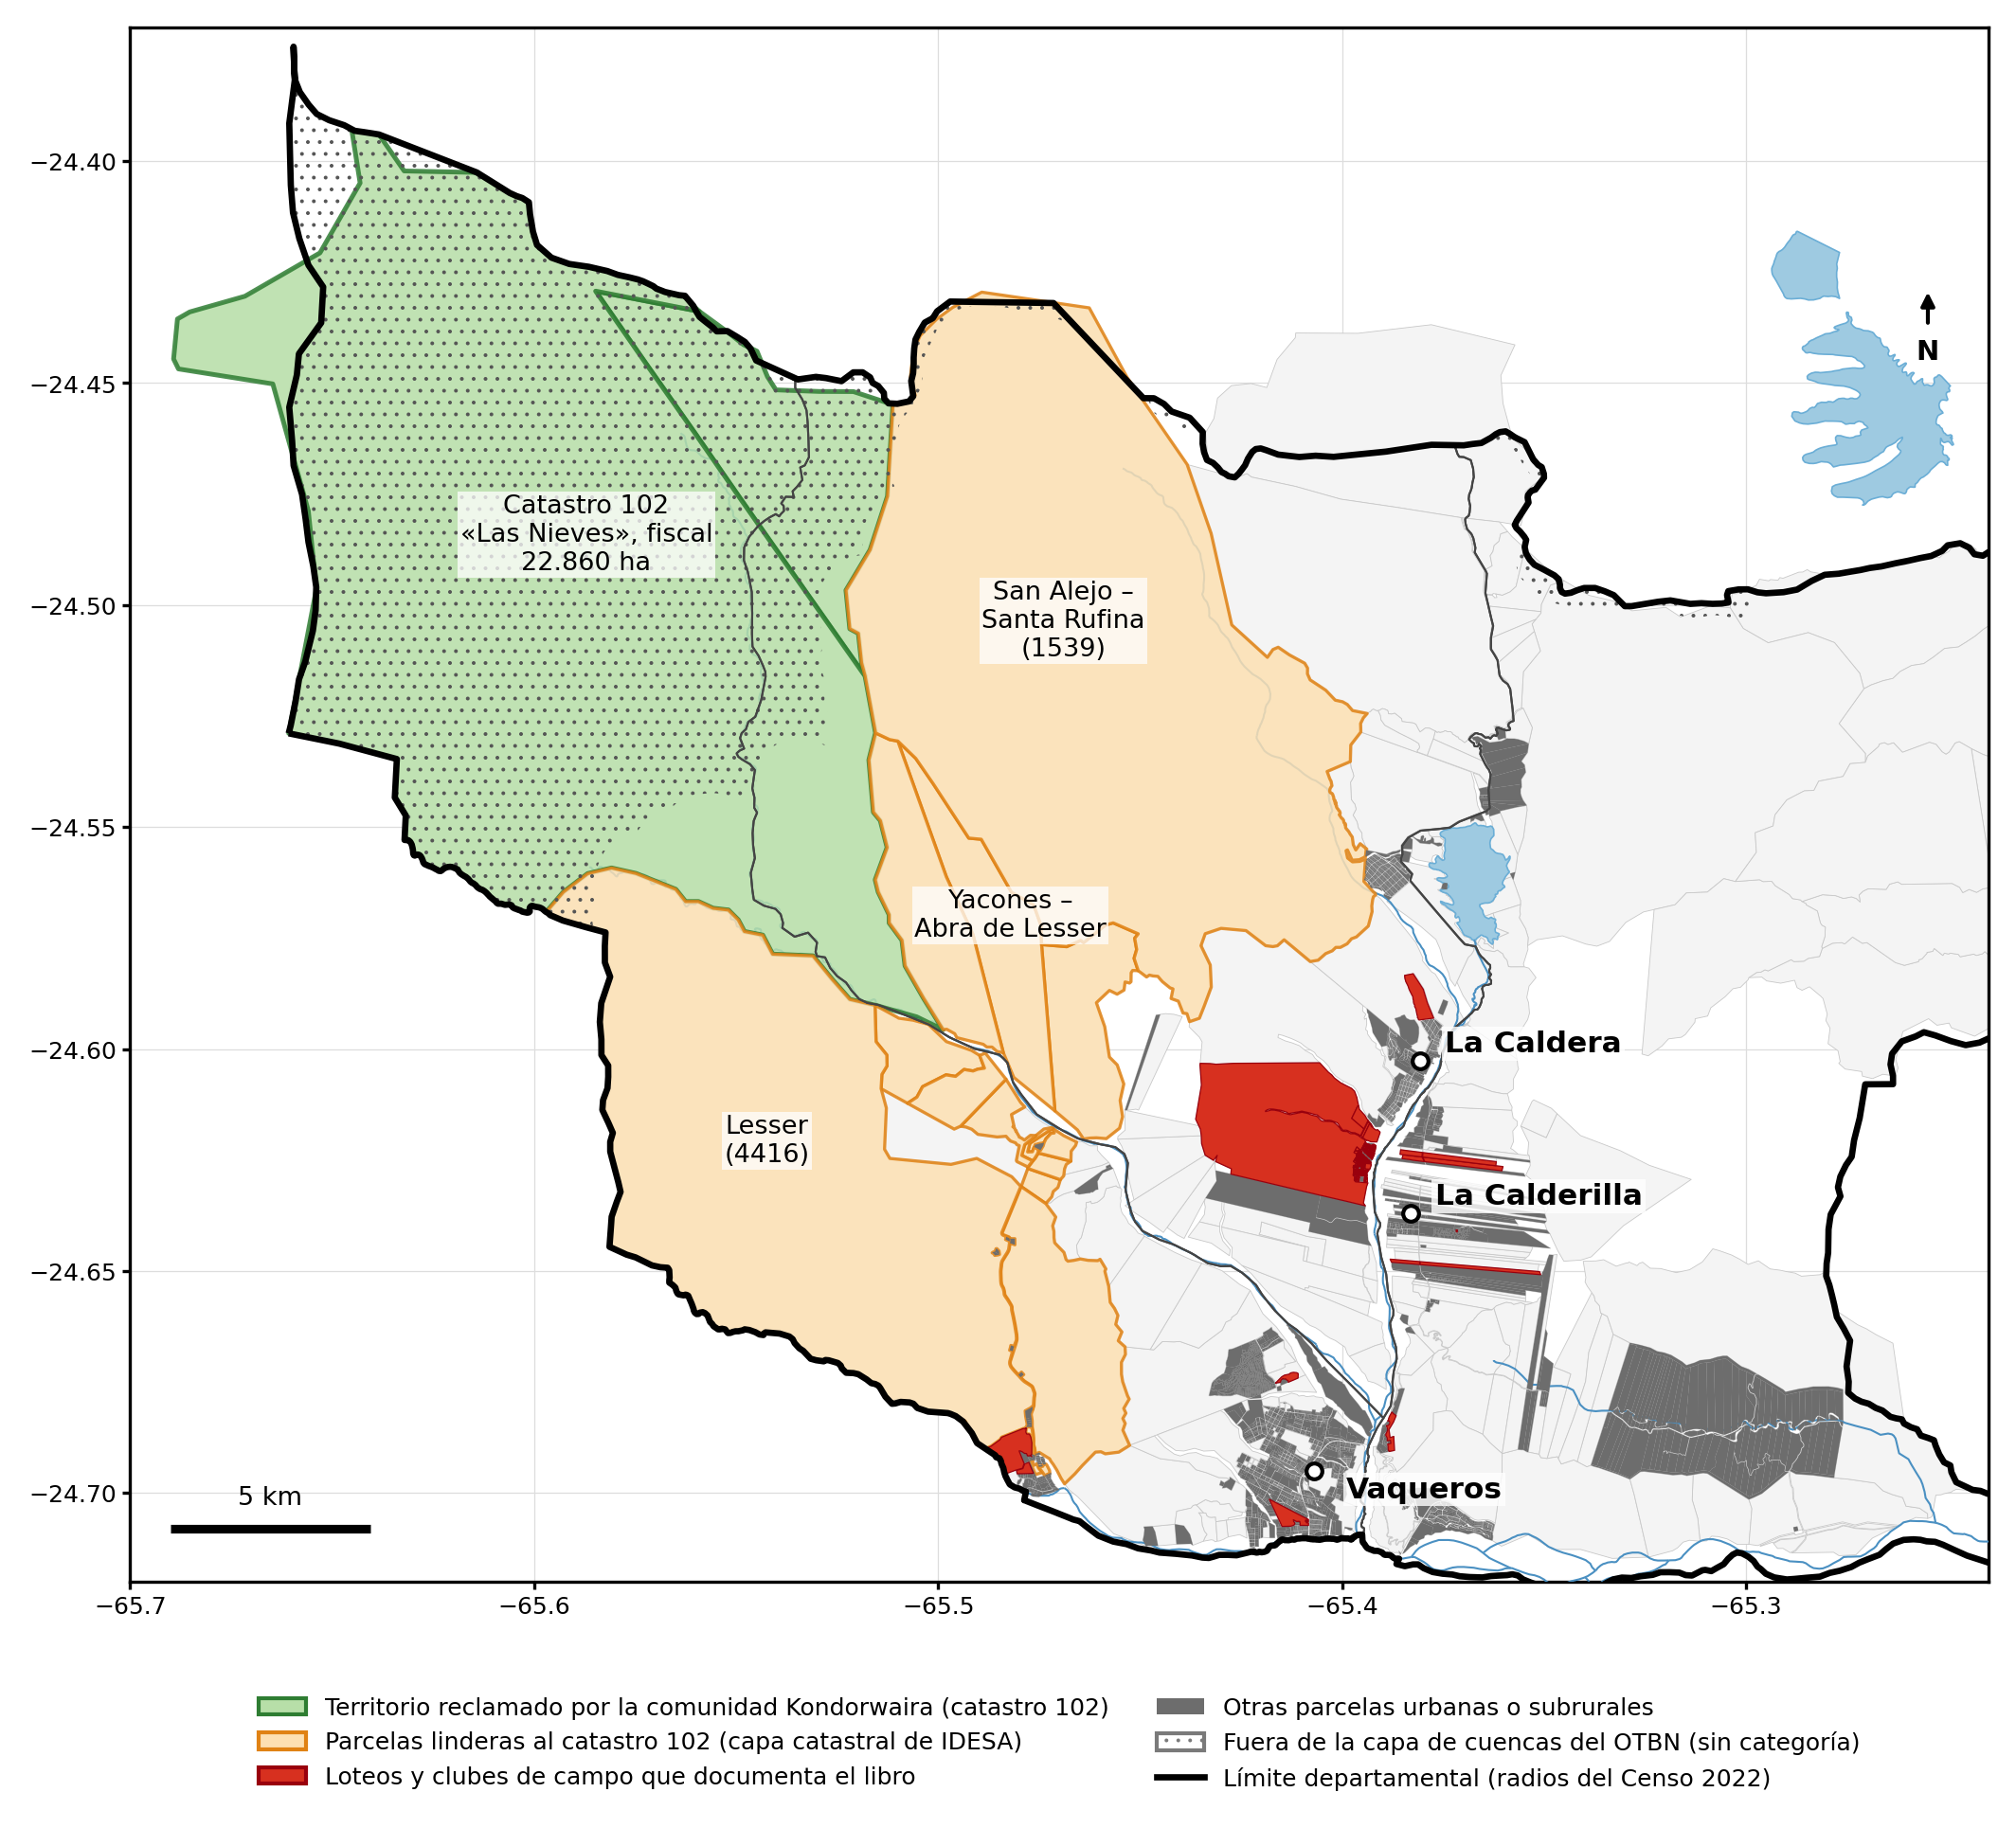
\includegraphics[width=\textwidth,height=0.80\textheight,keepaspectratio]{fig-kondorwaira-catastro.png}
\caption[El territorio reclamado por la comunidad Kondorwaira y los loteos del libro]{\textbf{El territorio reclamado por la comunidad Kondorwaira y los loteos del libro.} En verde, el catastro 102, «Las Nieves», que Pérez Domínguez y Belmonte (2024) identifican como el territorio reclamado en la carpeta técnica; en naranja, las parcelas que lo lindan según la capa catastral; en rojo, los loteos y clubes de campo que documenta este libro; en gris oscuro, las demás parcelas urbanas o subrurales. La trama punteada marca lo que queda fuera de la capa de cuencas del informe técnico de la Ley 8483, es decir, sin categoría de bosque. Elaboración propia con la capa «Catastro Urbano y Rural» de la Dirección General de Inmuebles (geoportal de IDESA, descargada en septiembre de 2026; el organismo la declara orientativa), la cartografía de radios del Censo 2022 (INDEC, corregida por CEUR-CONICET), la capa de cuencas del informe técnico de la Ley 8483 y la hidrografía del IGN. Superficies en proyección equivalente (EPSG:6933). Elaboración propia; dibujo de \texttt{scripts/mapa\_kondorwaira.py} del repositorio \texttt{mapas\_caldera} (apéndice \ref{cap:fuentes}).}\label{fig:kondorwaira}
\end{figure}

\begin{ficha}{Catastro 102 y su entorno, sobre la capa catastral de IDESA}
\begin{itemize}[leftmargin=*,nosep]
\item \textbf{Catastro 102, finca «Las Nieves»}, categoría rural, plano Nº 2: \textbf{22.860 hectáreas} en dos polígonos. Es la parcela más grande del departamento y equivale a cerca de la quinta parte de su superficie.
\item \textbf{Radios censales:} 17.941 hectáreas caen en el radio rural 0101 de Vaqueros ---el 96,5 por ciento de ese radio, donde el censo contó setenta y ocho habitantes--- y 4.067 en el radio rural 0201 de la fracción de La Caldera. Unas 800 hectáreas quedan fuera del contorno censal del departamento, al oeste.
\item \textbf{Parcelas linderas:} San Alejo -- Santa Rufina (catastro 1539, 13.927 hectáreas, plano 120); Lesser (catastro 4416, 10.435 hectáreas, plano 936), y el fraccionamiento Yacones -- Abra de Lesser (catastros 3414 a 3418, plano 615).
\item \textbf{Loteos del libro:} ninguno toca el catastro 102 ni sus parcelas linderas. El más próximo es el remanente rural de El Durazno (catastro 6713), a 6,5 kilómetros; los lotes de El Durazno, el club de campo Finca Lesser, La Milagrosa y El Nogalar están a más de diez. La parcela urbana o subrural más cercana de cualquier clase es una de 2,5 hectáreas (catastro 3419) dentro del fraccionamiento Yacones -- Abra de Lesser, a 3,7 kilómetros.
\end{itemize}
\textit{Distancias medidas entre bordes de parcela en coordenadas UTM 20 S. Los catastros 4366, 3709, 4065, 3616, 1713 y 1905 ya no figuran en la capa: se subdividieron, y sus derivados entran en el cálculo por su número actual cuando el libro lo conoce.}
\end{ficha}

\begin{cautela}
\textbf{Lo que el cruce contesta y lo que no.}

\textbf{Contesta la pregunta tal como estaba formulada, a nivel de catastro, y la respuesta es negativa}: ninguno de los fraccionamientos que este libro documenta se superpone con la parcela que la carpeta técnica reclama, ni con las que la rodean. Los loteos están en el valle; el territorio comunitario, en la cabecera, del otro lado de las fincas grandes.

\textbf{No contesta el perímetro fino.} La carpeta técnica puede reclamar más o menos que la parcela catastral, y el artículo registra que la vida de la comunidad se extiende también a fincas privadas colindantes. La capa, además, es orientativa. La respuesta definitiva sigue en la cartografía de la carpeta.

\textbf{Y deja una pregunta nueva, que mira hacia adelante.} El catastro 1539, San Alejo -- Santa Rufina, lindero al territorio por el este, es la matrícula donde \textsc{agro san alejo s.a.s.}\ fijó su sede en enero de 2026, con un objeto que incluye el turismo rural y los desarrollos inmobiliarios (capítulo \ref{cap:trabajo}). Este libro no sabe si la sociedad es titular o arrendataria de la finca, ni qué piensa hacer en ella. Pero si el próximo fraccionamiento del departamento ocurre ahí, ocurrirá sobre una finca donde, según el artículo, la comunidad también vive y pastorea.
\end{cautela}

\subsection*{Qué contiene una carpeta técnica, y dónde está}

El relevamiento de la Kondorwaira se aprobó por la Resolución INAI Nº 617/2013. Este libro no
tiene esa resolución, pero sí el modelo: las resoluciones de relevamiento del INAI tienen
todas la misma estructura, y una de ellas permite saber exactamente qué documentos existen
detrás de la de 2013 y dónde buscarlos.

\begin{ficha}{Estructura de una resolución de relevamiento del INAI --- Ley 26.160}
El \textbf{artículo 1} da por cumplido el Relevamiento Técnico, Jurídico y Catastral.

El \textbf{artículo 2} «reconoce la ocupación actual, tradicional y pública» de la comunidad
«respecto de la \textbf{superficie georreferenciada, que figura como ANEXO I} y forma parte
integrante de la presente medida».

Y al pie: «El/los \textbf{Anexo/s} que integra/n esta Resolución \textbf{se publican en la
edición web} del Boletín Oficial de la República Argentina».

Los considerandos enumeran las piezas de la \textbf{carpeta técnica}: acta de consentimiento
de la comunidad; \textbf{Cuestionario Socio-Comunitario Indígena}; \textbf{Narrativa} y
\textbf{Croquis}; \textbf{cartografía georreferenciada} con demarcación de los usos internos y
del perímetro; \textbf{Informe Histórico Antropológico}; \textbf{Dictamen Jurídico} con
estrategias de regularización dominial según «la situación registral en que se encuentra el
territorio georreferenciado»; e \textbf{Informe Técnico Final}.
\end{ficha}

Tres consecuencias, y la primera explica por qué el pedido más importante de este libro es difícil de satisfacer.

\textbf{Primera: el perímetro georreferenciado existe, pero probablemente no sea público.} Las resoluciones más recientes de esta clase incorporan la superficie georreferenciada como Anexo I; no se sabe si la de 2013 lo publicó, y la búsqueda de este libro no la encontró (véase la última cautela del capítulo). Además, el convenio de 2022 entre el INAI y el Ministerio de Desarrollo Social de Salta, publicado como anexo del Boletín provincial, declara \textbf{secreta} toda la información del programa de relevamiento, en los términos de la Ley 24.766, y reserva al INAI con exclusividad el derecho de publicarla. \textbf{La vía realista para conocer la cartografía es la propia comunidad.} Con esa cartografía puede establecerse si alguno de los loteos que este
libro documenta se superpone con territorio de ocupación tradicional.

\textbf{Segunda: existe un dictamen jurídico sobre la situación registral del territorio.} La
carpeta técnica incluye, por diseño, un análisis de quién figura como titular registral de
las tierras relevadas y qué estrategias caben para regularizarlas. \textbf{Es, para la zona
alta de esta cuenca, el informe de dominio que el capítulo \ref{cap:loteo} reclama para las matrículas del
loteo} --- hecho por el Estado nacional y diez años antes.

\textbf{Y tercera: el reconocimiento no es declarativo de propiedad.} El artículo 2 reconoce
la \textit{ocupación}, no titula. La Ley 26.160 declara la emergencia y suspende desalojos;
la propiedad comunitaria requiere una ley que el Congreso no dictó. \textbf{Lo que existe
sobre la zona alta de esta cuenca es un reconocimiento estatal de ocupación, no un título}, y
este libro no debe leerlo como si lo fuera.

\subsection*{Tres precisiones del expediente}

\textbf{El relevamiento tiene fecha exacta: 20 de noviembre de 2011.} El informe de 2023 lo califica de \textbf{«centralizado»}, y una primera lectura de este libro entendió que lo había hecho el equipo del INAI en forma directa. La carpeta técnica se aprobó por Resolución INAI Nº 617/2013.

El informe del 10 de agosto usa la palabra para la ejecución ---«fue realizado por el equipo técnico del INAI»---, pero el dictamen del 4 de septiembre, en el mismo expediente, lo atribuye al «área de DESCENTRALIZADA del INAI». Como se dijo más arriba, este libro no puede establecer cuál de los dos tiene razón.

\textbf{La segunda comunidad tramita su personería desde 2018 y el trámite está en el
Instituto Provincial de Pueblos Indígenas.} Cinco años después de iniciado, el expediente
54-142017/2018-0 seguía ahí en agosto de 2023.

\textbf{Y la tercera es la que más dice, aunque no hable de comunidades sino del Estado.}

Quien pidió el informe fue la \textbf{abogada de la Fiscalía de Estado de la Provincia}, en
representación de la propia Provincia demandada, y lo pidió «en carácter urgente»,
acompañando «mapa imagen satelital del área respectiva». El pedido dice, textualmente, que se
informe «si en la zona \textbf{se encuentra relevado} la existencia de comunidades
aborígenes».

Es decir: \textbf{en agosto de 2023, para saber si había comunidades en la cuenca que estaba
obligada a ordenar, la Provincia tuvo que preguntarse a sí misma}, girando el expediente de
un ministerio a otro y adjuntando una imagen satelital para que le identificaran el área.

El dato existía desde 2011 y estaba aprobado por resolución desde 2013. \textbf{No fue
necesario producirlo: fue necesario encontrarlo.} Y lo encontró, en una semana, una dirección
de otro ministerio de la misma provincia.

Este libro sostiene en el capítulo \ref{cap:opacidad} que la opacidad de este dispositivo rara vez consiste
en negar un documento. Aquí hay una variante que no había registrado: \textbf{un organismo del
Estado que no sabe lo que otro organismo del mismo Estado tiene documentado hace doce años.}

\begin{cautela}
Lo que este libro puede afirmar ahora y lo que sigue sin poder afirmar.

\textbf{Puede afirmar} que las comunidades existen, que están registradas, que su territorio
está relevado y aprobado, y que fueron convocadas a los talleres del Plan.

\textbf{No puede afirmar} cuántas personas las integran, qué superficie abarca el relevamiento
de 2011 ---la prensa oficial habla de veintisiete familias--- ni si el Plan aprobado recoge lo que las comunidades plantearon en la consulta, cuya acta transcribe el capítulo \ref{cap:amparo}.
Sobre la superposición con los loteos, el cruce catastral de este mismo capítulo da una respuesta negativa a nivel de parcela; el perímetro fino sigue en la carpeta técnica, y la finca lindera de San Alejo es, desde 2026, \textbf{la pregunta abierta más importante de este trabajo}.

El capítulo \ref{cap:infraestructura}, más adelante, enuncia como una de sus cuatro condiciones de refutación que aparecieran comunidades con ocupación anterior al archivo. \textbf{Aparecieron, aunque con un reconocimiento estatal de ocupación y no con un título.} Lo que la
tercera tesis decía --- que el mercado encontró un dispositivo armado --- hay que leerlo ahora
sabiendo que sobre ese mismo territorio había, además, una ocupación anterior a todo el
archivo que este libro recorrió.
\end{cautela}

\subsection*{Quince años de reclamo}

La cobertura consigna antecedentes de reclamo vecinal en La Caldera por la protección de los ríos y su entorno desde 2010: protestas, notas y denuncias ante la entonces Secretaría de Ambiente provincial y ante el municipio, y finalmente amparos colectivos.

La cronología del apéndice \ref{cap:cronologia} permite reconstruir la progresión: reclamos desde 2010, advertencia administrativa en 2016, la gacetilla de octubre de 2018 que este capítulo transcribe, denuncia pública en 2019, acción judicial en 2019, sentencia favorable en 2021, y ejecución litigada entre 2022 y 2026. Es, en escala municipal, el recorrido completo de los grados de disidencia que el libro anterior describió.

\section{Lo que resultó eficaz}

\textbf{El amparo colectivo ambiental.} Obtuvo lo que once años de gestión administrativa no habían obtenido: una condena a confeccionar un plan ---cuyo alcance sobre la ejecución de obras discuten las partes (capítulo \ref{cap:amparo})---, con criterio técnico definido por el tribunal y seguimiento judicial de la ejecución.

\textbf{La producción de conocimiento técnico independiente.} Una vecina con formación en biología produjo el registro público más citado del proceso de desmonte, sosteniendo que el negocio inmobiliario operaba sin control y con consecuencias de gravedad impredecible. Ese registro fue levantado por prensa nacional y funcionó como pieza de legitimación del reclamo.

\textbf{La peritación profesional colegiada.} El Consejo Profesional de Agrimensores, Ingenieros y Profesiones Afines actuó como veedor en la etapa de ejecución y recibió reconocimiento expreso del tribunal.

\textbf{El perfil de quienes litigaron.} El capítulo \ref{cap:poblacion} ubica al loteo El Durazno en el radio 0208 o en el 0209, y cualquiera de los dos está entre los de mayor formación del municipio: 21 y 24 personas con estudios universitarios por cada cien adultos, por encima de la capital, que tiene 16,7; en el 0209, más de la mitad de los adultos cursó un terciario o una carrera universitaria. El conjunto de la fracción queda en tres de cada diez \textit{contando el terciario} ---y en 13,6 si se cuentan sólo los universitarios---, y el radio más poblado del municipio, en 5 universitarios por cada cien. De modo que el nivel educativo del entorno de El Durazno es alto, sea cual fuere el radio. Con las reservas de aquel capítulo ---radios de 125 y 150 habitantes, propietarios de fin de semana que no se cuentan allí y barrios ubicados por inferencia---, los loteos que sostuvieron siete años de amparo parecen ser los que tenían, en proporción, más herramientas para hacerlo. No todos: El Nogalar, de origen municipal, también es parte actora, y este libro no sabe quiénes lo habitan.

\begin{cautela}
El rasgo compartido es la independencia estructural respecto del aparato local. Ni el amparista, ni la científica, ni el colegio profesional dependen del municipio para su reproducción material o simbólica. Es el mismo principio que el libro anterior formuló al cerrar su inventario de disidencias no absorbidas: lo que el dispositivo no puede absorber es aquello que no necesita su reconocimiento para existir.

El dato del censo agrega un matiz que conviene no omitir: esa independencia también tiene una base social. Que los más formados resistan mejor no le quita mérito a su resistencia, pero sí advierte sobre los ausentes. Los barrios del pueblo con menos formación sufrieron el mismo río y no aparecen en ningún expediente.
\end{cautela}

\section{Los límites}

Conviene no escribir una épica. El amparo de Vaqueros contra el loteo eclesial fue rechazado en 2019 y el emprendimiento avanzó. El amparo de La Caldera fue ganado en 2021 y las inundaciones volvieron en enero de 2026, semanas antes de que el plan fuera finalmente aprobado. Los reclamos por agua potable en la zona alta de Vaqueros llevan más de quince años sin resolución. El derrumbe de ladera sobre la ruta y las denuncias del centro vecinal de La Calderilla muestran que el frente de desmonte no se detuvo. Y el capítulo \ref{cap:amparo} documentó que la condena reapareció, cuatro años después, como propuesta de gestión del propio condenado.

\begin{cautela}
Una sentencia favorable obtenida contra un municipio sin capacidad técnica ni recursos para cumplirla produce una obligación, no un resultado. Ése es el límite estructural de la vía judicial en esta escala, y el libro no debe disimularlo.

De ahí se sigue una consecuencia práctica para quien litigue: el objeto útil de un amparo en este departamento no es sólo la condena al municipio, sino la condena a la Provincia a proveerle los medios. La Fiscalía de Estado ya estableció, en el propio expediente, que la responsabilidad de las obras es municipal porque el municipio autoriza. Falta que alguien establezca con qué debe hacerlas.
\end{cautela}

\section{Los ausentes}

Ninguno de los siguientes sujetos aparece en la cobertura periodística relevada, ni como parte en los expedientes identificados, ni en la literatura académica consultada: la población rural preexistente; los trabajadores de la construcción de los propios loteos; los ocupantes sin título; y las familias con posesión veinteañal no comunitaria. Las comunidades originarias estuvieron en esta lista hasta que el expediente de Fiscalía de Estado permitió sacarlas de ella.

\begin{cautela}
Su ausencia del corpus no prueba su ausencia del territorio. El libro anterior documentó, para otros departamentos, exactamente ese mecanismo: la invisibilidad documental como primer paso de la invisibilidad jurídica.

La diferencia entre ``verifiqué y no hay'' y ``no encontré'' es todo el método de este libro. Para las comunidades originarias ese paso ya se dio: existen y están registradas, como documenta el comienzo de este capítulo. Para los otros ausentes de la lista, todavía no.

Hay, sin embargo, dos rastros que conviene retener.

El primero es cuantitativo y el capítulo \ref{cap:tierra} lo documenta: el Censo Nacional Agropecuario 2018 registra en el departamento sesenta y una explotaciones agropecuarias sin límites definidos, el 46,6 por ciento del total, contra el 32,8 provincial. Esa categoría no equivale a tenencia irregular, pero es el rastro estadístico más próximo a la población que este apartado nombra como ausente.

El segundo es cartográfico y es más directo. El informe técnico de la Ley 8483 establece que el criterio 11 de la Ley 7543 --- ``valor y uso dado por comunidades indígenas y campesinas a áreas boscosas o colindantes'' --- funciona como \textbf{capa de control de gestión}, y produce un mapa específico, identificado como Mapa 11 en el Anexo IX del informe. Cada proyecto de manejo o cambio de uso del suelo debe someterse a un protocolo de consulta previa, libre e informada, y no puede aprobarse sin el visto bueno de las Comisiones de Evaluación conformadas para aplicarlo.

Existe, por lo tanto, un mapa oficial y público que registra dónde hay comunidades indígenas y campesinas en la provincia de Salta. Consultado para este libro, el mapa muestra el departamento bajo la mancha de uso potencial indígena, pero a su escala no permite saber si el territorio relevado de la Kondorwaira figura en él ni con qué alcance.

Hay, sin embargo, un dato del propio proceso que conviene poner junto a esa pregunta. El Consejo Asesor que produjo el ordenamiento clasificó a sus cincuenta y tres integrantes en siete tipos, y el séptimo --- \textit{representantes de pueblos originarios} --- registra \textbf{cero}, según el informe técnico que integra el Anexo I de la Ley 8483. En el taller del 25 de octubre de 2023, en cambio, se acreditaron diecisiete representantes de pueblos originarios, casi uno de cada cinco participantes: la ausencia es de instituciones indígenas en el Consejo, no de personas en el taller.

Un libro que se pregunta por los ausentes de su territorio encuentra, en el instrumento provincial que debía identificarlos, la misma ausencia formalizada en una tabla.
\end{cautela}

\section{Una asociación anterior al conflicto}

Entre las convocatorias a asamblea que publica el Boletín Oficial aparece una entidad que este libro no había registrado y que importa por su fecha.

\begin{ficha}{Convocatoria a asamblea ordinaria --- B.O.\ Nº 19.430, 19 de noviembre de 2014}
La \textbf{``Asociación de Vecinos de los Ríos Castellanos y Lesser''} convoca a sus socios a asamblea ordinaria para el 23 de diciembre de 2014, en calle M.\ Julia Solá 309 de \textbf{Lesser}, para considerar memoria, balance, inventario e informe de la comisión revisora de cuentas, y \textbf{elegir todos los miembros} de la comisión directiva y de la revisora de cuentas.

Firman por la comisión directiva \textbf{Inés Ortíz de Cárdenas} y \textbf{José Armando Caro Figueroa}.
\end{ficha}

\begin{cautela}
Tres puntos que este dato aporta al capítulo.

\textbf{La primera es cronológica.} En noviembre de 2014 existía en el departamento una asociación civil con personería, comisión directiva, órgano de fiscalización y balance anual, \textbf{organizada explícitamente alrededor de dos ríos}. Cuatro años antes del primer aluvión y más de cuatro antes del amparo colectivo. La organización vecinal en torno al agua no nació del desastre: lo precedía.

\textbf{La segunda es de escala.} Los ríos Castellanos y Lesser corresponden a parajes del departamento que este libro apenas menciona, y que no figuran en ninguno de los conflictos documentados. Que allí hubiera vecinos asociados y renovando autoridades sugiere que el tejido asociativo del corredor es más denso de lo que la reconstrucción por conflictos permite ver. Un libro que sigue litigios ve sólo donde hubo litigio.

\textbf{La tercera es un nombre.} Uno de los firmantes, \textbf{José Armando Caro Figueroa}, es homónimo de quien fuera Ministro de Trabajo de la Nación entre 1993 y 1997, salteño de origen. Este libro \textbf{no afirma que sean la misma persona}: comparte nombre completo, lo que es indicio y no prueba, y la coincidencia se resuelve con un padrón, no con una lectura. Se consigna porque, de confirmarse, indicaría que la asociación de vecinos de esos ríos contaba con integrantes de peso institucional considerable, y eso cambiaría la lectura de su capacidad de acción.
\end{cautela}

Y el relevamiento de los boletines de 2015 confirma la densidad. En marzo aparecen convocando a asamblea la \textbf{Liga Municipal de Fútbol San Lorenzo -- La Caldera}, con sede en avenida San Martín de Vaqueros, tratando balances de los períodos 2010 a 2013 y la incorporación definitiva de clubes; y el \textbf{Club Social y Deportivo de Caza y Pesca La Caldera}, que sesiona en el local del Centro de Jubilados Cristo Monumental, en calle Las Margaritas y Madreselva. Con la Asociación de Vecinos de los Ríos Castellanos y Lesser, el Centro de Jubilados de Vaqueros y la Asociación Civil CESPS --- que en enero de 2015 renovaba comisión directiva en General Güemes 250 de Vaqueros ---, son al menos cinco entidades con personería y vida asamblearia en un departamento que hoy tiene doce mil habitantes.

Dos observaciones. \textbf{La primera:} el nombre de la liga de fútbol --- San Lorenzo y La Caldera juntos, con sede en Vaqueros --- vuelve a mostrar que el corredor funciona como una unidad social que ninguna jurisdicción administra entera. Lo que el capítulo \ref{cap:redes} documentó para el transporte y para el río, la liga de fútbol lo resolvió sola en 2015.

\textbf{La segunda:} varias de esas asambleas tratan balances atrasados de tres y cuatro ejercicios. Es un rasgo común de las entidades pequeñas y no indica irregularidad, pero sí que la vida asociativa del departamento es real y a la vez precaria: existe, se sostiene y le cuesta cumplir sus propias formas.

\begin{cautela}
Dos entidades más, y una de ellas obliga a mirar el capítulo \ref{cap:tierra} de otra manera.

En junio de 2015 convoca a asamblea la \textbf{Asociación Civil de Pequeños Productores Agropecuarios del Departamento La Caldera}, con sede en calle Las Moreras 587 del municipio de Vaqueros, para tratar memoria y balances de 2013 y 2014 y renovar autoridades. Firma como secretario el Dr.\ Diego A.\ M.\ Ragone.

\textbf{Existían pequeños productores agropecuarios organizados en el departamento en 2015}, y su asociación siguió convocando asambleas al menos hasta 2024 (capítulo \ref{cap:ausencias}). El capítulo \ref{cap:tierra} documenta que entre 2002 y 2018 el departamento perdió el 88,4 por ciento de su superficie agrícola, mientras la provincia ganaba terreno. Ese desplome no ocurrió sobre un vacío: ocurrió sobre productores que tenían asociación con personería, órgano de fiscalización y cuota social.

Este libro no sabe cuántos eran, qué producían ni qué fue de ellos. Pero la existencia de la entidad cambia el modo de formular la pregunta del capítulo \ref{cap:tierra}. Ya no es ``qué pasó con las hectáreas'': es \textbf{qué pasó con la gente que las trabajaba}, y hay un registro donde empezar a averiguarlo.

La otra entidad es el \textbf{Club de Regatas Güemes}, cuya sede está \textbf{en el Dique Campo Alegre}. Es decir, sobre el espejo de agua que la Ley 4486 hizo posible expropiando cinco propiedades en 1972, y en cuyo entorno el municipio proyectaba en 2026 un ``nuevo circuito turístico''. Un club náutico con comisión directiva y balances, instalado en el embalse desde hace décadas, es un actor del área que este libro no había registrado como tal: el capítulo \ref{cap:tierrafiscal} documenta el permiso precario de 1980 a otro club náutico del perilago, el Club de Regatas Campo Alegre, y no establece si son la misma entidad con otro nombre.
\end{cautela}

\section{Un Estado que sí llega: la mediación comunitaria}

\begin{ficha}{Decretos Nº 475 y 481 del 9 de febrero de 2015 --- B.O.\ Nº 19.485}
El Ministerio de Justicia prorroga por doce meses, a partir del 1 de enero de 2015, los contratos de locación de servicios de \textbf{dos mediadoras comunitarias} que se desempeñan en el \textbf{Centro de Mediación Comunitaria de La Caldera}: \textbf{Mariángeles Giraldez}, cuyo contrato se aprobó por Decreto 3722/09, y \textbf{Flavia del Valle Tabarcache}, por Decreto 3871/10.

Ambos contratos dependen de la Secretaría de Métodos Alternativos de Resolución de Conflictos.
\end{ficha}

\begin{cautela}
Es un dato pequeño y corrige un sesgo de este libro.

El departamento tiene, desde 2009 y 2010, un \textbf{Centro de Mediación Comunitaria} con dos profesionales contratadas por la Provincia y renovadas año tras año. Existe también, según los mismos boletines, un centro equivalente en Vaqueros. Es decir: hay una política pública provincial de resolución de conflictos instalada en el territorio, sostenida durante más de un lustro.

Este libro se construyó siguiendo litigios, desmontes y expedientes de aprobación, y esa elección produce una imagen del Estado que llega tarde o no llega. La mediación comunitaria es un caso donde llegó, se quedó y se renovó. No hace falta que eso equilibre el balance --- no lo equilibra ---, pero sí que quede registrado, porque un libro que sólo mira donde hubo conflicto termina describiendo un Estado que sólo existe en el conflicto.

Lo que no sabemos es qué se medió. Un centro de mediación comunitaria en un departamento donde se disputan tierras, aguas y loteos pudo intervenir en cualquiera de esos frentes, o en ninguno. Sus registros lo dirían.
\end{cautela}

\section{Áridos sobre tierra fiscal}

\begin{ficha}{Edicto de mina --- Expte.\ Nº 18.219, publicado en enero y febrero de 2014}
El Juzgado de Minas y en lo Comercial de Registro, a cargo del Dr.\ Daniel Enrique Marchetti, hace saber que \textbf{Transporte Hnos.\ Mendoza S.R.L.} solicitó la publicación de la \textbf{renovación de concesión} de la cantera de áridos denominada \textbf{``Macarena''}, ubicada en el departamento La Caldera, \textbf{lugar río Wierna}.

Superficie libre: \textbf{10 hectáreas}. Coordenadas Gauss Krüger, sistema Posgar 94 y Campo Inchauspe/69.

\textbf{``Los terrenos afectados son de propiedad Fiscal.''}
\end{ficha}

\begin{cautela}
Es el primer edicto minero del departamento que este relevamiento encontró para el período 2014--2015, y reúne tres hilos que este libro llevaba separados.

\textbf{El primero:} hay extracción de áridos concesionada sobre el río Wierna, uno de los cursos que --- según el testimonio vecinal recogido en el capítulo \ref{cap:expropiacion} --- rodean Vaqueros y cuya agua los vecinos no reciben.

\textbf{El segundo:} el artículo 171 del Código de Aguas exige que, \textbf{antes} de otorgar permisos de extracción de áridos, la Autoridad de Aplicación evalúe si afectarán desfavorablemente las riberas o el flujo de las aguas, y en su caso desaconseje el otorgamiento o exija obras. Una \textbf{renovación} de concesión es una nueva instancia de otorgamiento. Si esa evaluación se hizo, está en el expediente.

\textbf{Y el tercero, que es el que más pesa:} los terrenos son de \textbf{propiedad fiscal}. Diez hectáreas de tierra pública en un departamento donde, según el capítulo \ref{cap:tierrafiscal}, el circuito de adjudicación de tierra fiscal a familias tarda décadas y exige nacionalidad, cuatro años de residencia y no poseer inmuebles en ningún lugar del mundo. La misma tierra pública se concesiona para extraer áridos con un edicto de tres publicaciones.

Este libro no compara los dos regímenes para reprochar el segundo: la concesión minera y la adjudicación social son institutos distintos, con finalidades distintas, y ninguno es ilegítimo. Los compara porque \textbf{ésa es exactamente su tesis}: sobre el mismo suelo público operan dos circuitos con intensidades regulatorias inversamente proporcionales a la capacidad de sus beneficiarios.
\end{cautela}

En febrero y marzo de 2014, casi en simultáneo con el edicto de «Macarena», el mismo juzgado publicó el edicto de renovación de la cantera de áridos \textbf{``El Vaquero''}, expediente 19.199/08, solicitada por \textbf{INCOVI S.R.L.}, ubicada en el departamento La Caldera, lugar Vaqueros, con una superficie de \textbf{nueve hectáreas y 347 metros cuadrados}. También allí: ``los terrenos afectados son de propiedad Fiscal''.

Y hay una tercera, sobre el mismo curso aunque del otro lado del límite: en abril de 2014 se publicó la renovación de la cantera \textbf{``El Triunfo II''}, expediente 17.422, solicitada por la \textbf{Cooperativa de Provisión de Áridos La Mesa Redonda Ltda.}, ubicada ``en el departamento Capital, río La Caldera''. El yacimiento está en la Capital; el río es el mismo.

Tres concesiones de áridos sobre la misma cuenca en un solo trimestre, dos de ellas sobre \textbf{tierra fiscal} dentro del departamento y sumando casi veinte hectáreas. Las dos primeras por renovación, con antecedentes que se remontan al menos a 2008.

Y la tercera agrega el dato jurisdiccional que el capítulo \ref{cap:vaqueros} ya había encontrado por otra vía: el río La Caldera y su continuación atraviesan dos departamentos, y la extracción de áridos se autoriza a ambos lados sin que ningún organismo tenga competencia sobre el conjunto del cauce.

El contraste con el circuito de adjudicación social: son las mismas hectáreas fiscales, la misma provincia y el mismo año.

Y no es una sola cantera. Para noviembre de 2015 el relevamiento suma \textbf{seis concesiones de áridos} en la cuenca ---una de ellas en jurisdicción de la Capital---: ``Macarena'' (Transporte Hnos.\ Mendoza, río Wierna, 10 ha fiscales), ``El Vaquero'' (INCOVI, Vaqueros, 9 ha fiscales), ``El Triunfo II'' (Cooperativa La Mesa Redonda, río La Caldera, jurisdicción Capital), \textbf{``Los Yacones''} (INCOVI, cauce del río Wierna, \textbf{21 ha 6.374 m² de terrenos fiscales}) \textbf{``Don Roque I''} (M.E.I.\ Obras y Servicios S.R.L., río Vaqueros) y \textbf{``Joaquín''} (René Antonio Barranco Barrera, río Las Nieves).

Con ``Los Yacones'', \textbf{INCOVI S.R.L.\ acumula dos canteras sobre tierra fiscal} --- más de treinta hectáreas entre ambas --- y es la cuarta aparición de esa firma en este libro, después de la cantera de Vaqueros, la oferta en la obra de protección del acueducto y la contratación directa para su reparación. Se consigna, como en los casos anteriores, sin atribuir irregularidad: una empresa de obra vial e hídrica que explota canteras de árido hace lo propio de su rubro.

\subsection*{Y hay minería propiamente dicha}

Las canteras de áridos no agotan la actividad extractiva del departamento.

\begin{ficha}{Mina ``Cristina M-1'' --- Expte.\ 22.295, publicado en abril de 2015}
El Juez de Minas hace saber que \textbf{Roberto Adrián Scasso, Julio Argentino Monteros, Facundo Martín Monteros Moya y Federico Joaquín Monteros Moya} manifestaron el descubrimiento de un \textbf{yacimiento de fosfatos} en el departamento La Caldera, distrito Mojotoro, \textbf{Sierra de Mojotoro}.

\textbf{Superficie concedida: 1.256 hectáreas 3.712 m².}

``Los terrenos son \textbf{privados}'': la matrícula 1.902 pertenece a \textbf{Jorge Raúl Sanz}; las matrículas \textbf{1.981, 1.982, 1.983, 1.984 y 1.985 pertenecen a TURPINAR S.A.}; y la matrícula 1.862 se encuentra sujeta a inscripción registral.

Plazo para que quienes tuvieren derechos los hagan valer: sesenta días.
\end{ficha}

Dos cosas, y la segunda excede a este capítulo.

\textbf{La primera: la escala.} Mil doscientas cincuenta y seis hectáreas es una superficie mayor que la de varios de los loteos y clubes de campo que este libro documenta juntos. Y no se trata de áridos de río sino de un yacimiento de \textbf{fosfatos}, un mineral de segunda categoría con destino industrial. La Sierra de Mojotoro, sobre el límite oriental del departamento, tiene entonces valor minero declarado.

\textbf{La segunda: aparece un propietario corporativo.} El edicto identifica a \textbf{TURPINAR S.A.} como titular de \textbf{cinco matrículas contiguas} --- 1.981 a 1.985 --- en la sierra. Es la primera vez que este relevamiento encuentra a una sociedad anónima concentrando esa cantidad de inmuebles en el departamento, y aparece por vía indirecta: no en un aviso societario ni en una aprobación de loteo, sino en la citación de un expediente minero de tercero.

Es exactamente el tipo de dato que el capítulo \ref{cap:opacidad} explica que no se encuentra: la propiedad concentrada no se publica, se deduce de actos que la mencionan de paso. Quiénes integran TURPINAR S.A., desde cuándo posee esas matrículas y qué superficie suman es materia de la Dirección General de Inmuebles y del legajo societario.

\begin{cautela}
Un resultado negativo de búsqueda, que no contradice lo anterior y conviene explicar. La búsqueda sistemática en buscadores públicos de resoluciones del Instituto Nacional de Asuntos Indígenas que den por cumplido el relevamiento técnico, jurídico y catastral de la Ley 26.160 en la provincia de Salta no arrojó ninguna correspondiente al departamento La Caldera. Las localizadas corresponden a Molinos, Cachi, La Poma, San Carlos, General San Martín y otros departamentos. En Salta esos relevamientos se ejecutaron, por regla general, mediante Equipo Técnico Operativo convenido entre el INAI y el ministerio provincial. La Resolución INAI 617/2013, que aprobó el de la Kondorwaira, se conoce por el informe del Equipo Técnico de 2023 y no apareció en esa búsqueda: es un ejemplo más de por qué este libro no convierte una ausencia en un buscador en una ausencia en el registro.

Lo que puede afirmarse es que no se localizó acto administrativo publicado de relevamiento en el departamento.

Hay además una fuente que contesta la pregunta por vía positiva y que este libro ya sabe procesar: el Censo 2022 publica, por departamento, la población que se reconoce indígena o descendiente de pueblos indígenas u originarios, con desagregación por pueblo a nivel provincial. Es el mismo camino de Redatam que el capítulo \ref{cap:poblacion} empleó para la vacancia habitacional.
\end{cautela}


\parte{La opacidad}
{No falta el acto: falta el criterio. Seis instrumentos que publican la envoltura y reservan a un anexo lo que permitiría verificarlos.}
\chapter{La capa fina}

\label{cap:opacidad}
\section{Un obstáculo que se repite}

Este capítulo no estaba previsto. Se impuso porque el mismo obstáculo apareció cinco veces, en instrumentos de dos niveles de gobierno distintos ---el municipal y el provincial---, siempre en el mismo lugar del procedimiento: el punto donde el acto pasa de enunciar a decidir.

\textbf{Una corrección que el propio capítulo debe poner al frente.} Cuatro de esos cinco anexos resultaron estar, después, en el repositorio del Boletín: uno escaneado con capa de texto y tres como imágenes escaneadas sin ella. El quinto, el reglamento de fraccionamiento de Vaqueros, apareció al final fuera del Boletín: en el digesto que el propio municipio publica en línea. Lo que este capítulo documenta son, entonces, dos cosas que al principio parecían una: \textbf{anexos que no se publican} y \textbf{anexos que se publican de un modo que nadie los encuentra}.

Lo que sigue es el inventario --- seis instrumentos, de dos niveles de gobierno, relevados a lo largo de todo este trabajo --- y después la interpretación.

\section{El departamento se catastró en 1929}

Este capítulo sostiene que la opacidad de este territorio está en el criterio y no en el
acto. Conviene empezar por establecer desde cuándo existe el registro que hoy no se puede
consultar sin arancel.

\begin{ficha}{Decreto Nº 10.910 del 5 de agosto de 1929}
Expediente 3463-D. Vista la nota del Director de la Comisión de Catastro elevando la
solicitud del señor \textbf{Adeodato Aybar\index{Aybar, Adeodato}}, «en la cual éste manifiesta que teniendo
urgente necesidad de la suma de \$500, y \textbf{habiendo terminado la catastración de los
Departamentos de Campo Santo, Caldera y La Viña}, pide se le liquide la citada suma a
cuenta de la remuneración que le sea fijada».

Se liquidan quinientos pesos al Director de la Comisión de Catastro para que los entregue
al catastrador, imputados a la Ley 9720.
\end{ficha}

De modo que el departamento La Caldera está catastrado desde 1929, y el trabajo lo hizo una
persona con nombre y apellido, a la que el Estado le debía la remuneración cuando terminó.

Ese dato tiene dos consecuencias para este libro.

La primera es que \textbf{el registro existe desde hace casi un siglo}. Cuando el capítulo \ref{cap:fincas} muestra mensuras que describen límites por «unos mojones antiguos», y cuando este libro
no puede establecer si una matrícula proviene de otra, no está describiendo un territorio
sin catastrar: está describiendo un territorio catastrado en 1929 cuyo catastro no es
consultable sin arancel ni presencia física.

La segunda es de escala, y explica algo del carácter de la información que quedó. Un solo
catastrador terminó tres departamentos y cobró quinientos pesos a cuenta. El presupuesto
municipal de La Caldera de 1908 era de mil cuatrocientos ochenta y tres; la casa quinta de
Lesser se remató en 1927 con base de seis mil. El levantamiento catastral de tres
departamentos costó, en pagos a cuenta, menos de la décima parte de una finca de diez
hectáreas.

\section{Los anexos sí se publican}

Este capítulo sostiene que seis instrumentos publican la envoltura y reservan el contenido
decisorio a un anexo. Corresponde precisar esa afirmación antes de desarrollarla, porque el
Boletín Oficial tiene, desde hace años, un repositorio de anexos.

\textbf{Existe una colección digital de anexos, separada de la del boletín.} Un relevamiento
de dieciséis anexos de octubre de 2017 arroja \textbf{trescientas veintiséis páginas} de
material: transferencias de partidas presupuestarias, incorporaciones de obra pública,
planillas de personal. La Caldera y Vaqueros aparecen ahí --- con código auxiliar, importe y
número de expediente --- en lugares donde el acto publicado en el boletín no los nombra.

De modo que \textbf{la afirmación de este capítulo no puede ser que los anexos no se
publiquen}. Se publican, y en volumen.

Lo que este libro documenta es más específico, y conviene enunciarlo con exactitud:

\begin{quote}
De seis instrumentos identificados cuyo contenido operativo está en un anexo o en la sede del organismo, \textbf{cinco no se obtuvieron por ninguna vía}, incluida la consulta
del repositorio. El sexto, el reglamento de fraccionamiento de Vaqueros, lo terminó publicando el propio municipio en su digesto en línea, no el Boletín que publicó el acto.
\end{quote}

La diferencia importa. No es que el Estado no publique anexos: es que \textbf{unos anexos se
publican y otros no, y no hay criterio visible que distinga a unos de otros}. Un anexo de
transferencia de partidas por quince mil quinientos noventa y cinco pesos con siete centavos
está disponible; el contrato de promoción turística que fija exenciones impositivas, no.

\begin{cautela}
Hay además un problema de acceso que conviene separar del de publicación, porque son
distintos y este libro los ha tratado juntos.

En ese mismo relevamiento de dieciséis archivos, \textbf{ninguno es un PDF pese a llevar esa
extensión}: trece son archivos comprimidos con una imagen y un texto por página, dos son
texto plano corrido sin marcas de página --- lo que impide citar por página cualquier
hallazgo que contengan --- y uno pesa trescientos catorce bytes, todos saltos de línea.
\textbf{Dos de los trece venían con la capa de texto enteramente vacía} y hubo que
reconocerlos ópticamente para poder leerlos.

Nada de eso es ocultamiento. Es infraestructura documental deficiente, y produce el mismo
efecto práctico: \textbf{el contenido está publicado y no es consultable sin trabajo técnico
previo}. Este libro lo consigna como lo que es --- una barrera de acceso, no una decisión de
reserva --- y lo distingue de los cinco contenidos que no se obtuvieron por ninguna vía.
\end{cautela}

\subsection*{Y un caso distinto: el acto y el acta, sin el detalle}

Los seis instrumentos de este capítulo publican el acto y reservan el anexo. El Decreto
1.889/16 publica las dos cosas, y conviene anotarlo porque completa el cuadro.

La ficha web del Boletín (Nº 19.913, 29/11/2016) trae el decreto: visto, considerandos,
articulado y refrendo. El repositorio de anexos ofrece, con el nombre del decreto, el
\textbf{Acta Acuerdo} del Plan de Mínimas y Encauzamiento 2016--2017 --- cláusulas,
mecanismo de pago, firmantes ---, escaneada desde el folio 3. Ninguna de las dos piezas
transcribe la fecha del decreto ni el número de expediente.

\textbf{De modo que se conocen el acto y el convenio, y no su contenido operativo.} Dentro
del convenio, las dos piezas que deciden --- los proyectos de obra y la distribución de fondos
por municipio --- se invocan como existentes y no se adjuntan.

Es la misma estructura en otro orden: \textbf{lo publicado permite saber que algo se decidió, y
no qué se decidió ni sobre qué río.}

\section{Seis instrumentos con el criterio afuera}

\begin{ficha}{Instrumentos cuyo contenido operativo no se publicó junto al acto}
\begin{itemize}[leftmargin=*,nosep]
\item \textbf{Ordenanza Nº 000437, Municipalidad de Vaqueros} (Boletín Oficial provincial, 15/01/2015). Aprueba el Reglamento de Fraccionamiento de Tierras. Publicado: cuatro artículos aprobatorios. No publicado: el reglamento, que contiene superficies mínimas, cesiones obligatorias, obras exigibles al loteador, procedimiento y condiciones ambientales. Al pie, el Boletín consigna que el anexo se encuentra para su consulta en sus propias oficinas («de esta reparación», dice el original), y la ficha web del instrumento no ofrece enlace «Ver anexo». Es el único de los cinco casos con que este capítulo empezó cuyo anexo no está en el repositorio del Boletín. \textbf{Obtenido en septiembre de 2026 del Digesto Jurídico Virtual de la Municipalidad de Vaqueros}, una carpeta pública en línea que el municipio ya anunciaba el 2 de febrero de 2024; su contenido se resume en el capítulo \ref{cap:vaqueros}.
\item \textbf{Resolución Nº 383/14, Secretaría de Recursos Hídricos} (edicto en los B.O.\ Nº 19.466 y 19.467, 21 y 22/01/2015; la ficha web no ofrece enlace «Ver anexo»). Aprueba la determinación de la línea de ribera en ambas márgenes de los arroyos El Durazno y Guaranguay, matrícula 4366, departamento La Caldera. Publicado: que la línea fue determinada. No publicado: \textbf{las coordenadas Posgar que indican dónde está}, que quedan ``a disposición de los interesados en la sede de la Secretaría''. Otro expediente de la misma sección, en la misma edición del Boletín, sí publica su tabla de coordenadas. \textbf{No obtenidas.}
\item \textbf{Decreto Nº 463/15} (09/02/2015; B.O.\ Nº 19.485). Ratifica el contrato de promoción turística con Proyecto 1 S.A.\ para ampliar el Hotel La Caldera. Publicado: el acto ratificatorio. \textbf{No publicado: el contrato}; al pie, la leyenda «anexo para su consulta en oficinas de nuestra repartición», la misma fórmula de la Ordenanza 437. No obtenido.
\item \textbf{Decreto Nº 3069/14} (14/10/2014). Ratifica el contrato de promoción turística con La Caldera S.A. Publicado: el acto ratificatorio. \textbf{No publicado: el contrato}, que fija los alcances de las exenciones impositivas concedidas; la ficha del decreto en la edición web del Boletín no ofrece enlace «Ver anexo». No obtenido.
\item \textbf{Resolución Nº 142/14}, Secretaría de Recursos Hídricos. Aprueba la determinación de línea de ribera de los ríos Mojotoro y La Caldera sobre la matrícula 3616, y la Resolución 236/14 la rectifica. Publicado: el acto y el inmueble. \textbf{No publicadas: las coordenadas}, ni las erróneas ni las corregidas, remitidas a la sede del organismo (avisos en los B.O.\ Nº 19.364 y 19.377, agosto y septiembre de 2014, sin enlace «Ver anexo»). Con la 383/14, son las dos únicas de las trece determinaciones de 2013--2015 referidas a inmuebles particulares ---las quince de la serie, menos la 467/15, que delimita un tramo de curso, y la 023/14, que recae sobre el pueblo y no sobre una matrícula--- que no las publicaron, y ambas recaen sobre suelo en proceso de loteo, aunque esa condición la comparten otras dos que sí las publicaron (capítulo \ref{cap:ribera}). No obtenidas.
\item \textbf{Informe técnico del inciso e}, que funda la contratación por vía abreviada del Plan de Manejo. Publicado: el encuadre legal. \textbf{No publicado: el informe}. No obtenido.
\end{itemize}
\end{ficha}

\begin{cautela}
De los seis, cinco no se consiguieron. Los que este libro sí consiguió resultaron estar publicados, y el sexto también: no donde lo publicó el acto, sino en el digesto del municipio que lo dictó. Desde 2018 la Ley 8126 obliga a los municipios a publicar sus ordenanzas en el Boletín Oficial y en internet (art.\ 79); Vaqueros lo cumple por su propia cuenta, el Boletín provincial sigue remitiendo a sus oficinas.

\textbf{La lista tenía trece, y ocho salieron de ella.} Los que quedan fueron verificados uno por uno en la edición web: ninguno ofrece enlace «Ver anexo». La nómina de adjudicatarios del Decreto 63/25, el Reglamento de Asignación de la Resolución 82/16, el baremo de la Resolución 8/16 y los procedimientos de la Resolución 9/16 fueron los primeros casos que este libro registró como anexos no publicados, y los obtuvo por otras vías. Estaban publicados: la edición web del Boletín ofrece cada uno como archivo vinculado al acto, bajo la leyenda «Ver anexo». Los tres del régimen de tierra fiscal, además, son copias certificadas escaneadas, sin capa de texto, que ningún buscador encuentra; con los de la Resolución 7/16, que no estaba en la lista, y los de la 567D/26, los anexos de ese régimen publicados sólo como imagen son cinco. El del Decreto 63/25 es un caso intermedio: también es una copia certificada escaneada, de cuatro folios, pero trae una capa de texto de reconocimiento óptico ---imperfecta, con números de expediente y documentos mal leídos--- que lo vuelve buscable. A ellos se sumaron después el anexo del Decreto 1682/19, que reglamenta la aprobación de todos los loteos de la provincia ---también vinculado al acto, y con texto legible---, el de la Resolución 023/14 de Recursos Hídricos, que resultó contener la línea de ribera del pueblo de La Caldera con sus 134 coordenadas, en una copia escaneada, los de la Resolución 567D/26, que este libro contaba como obtenidos por vía lateral y estaban vinculados al acto, y el convenio de licencias de conducir del Decreto 1433/15, también escaneado. Los ocho pasan a la columna de lo que el repositorio sí contiene ---los escaneados, a la de la barrera de acceso que el apartado anterior describe---, y confirman su advertencia: la frontera entre lo publicado y lo reservado no siempre está donde un lector la busca, y cada uno de los cinco restantes debe cotejarse contra ese repositorio antes de citarse como no publicado. El cotejo sumó, en cambio, un caso: el Decreto 463/15, gemelo del 3069/14, cuya ficha remite el contrato a las oficinas del Boletín con la misma fórmula que la Ordenanza 437. Con él, la lista queda en seis. Queda fuera, porque no es un anexo sino un acto entero, la Resolución SMyE 20/2022 que rige la zona de exclusión de canteras junto a las tomas de agua: no se publicó (capítulo \ref{cap:amparo}).

Los anexos no son secretos: existen, integran los actos y son accesibles por pedido o por vías laterales. Lo que ocurre es que la publicidad legal se cumple sobre la envoltura y la publicidad efectiva queda a cargo del interesado. Quien tiene tiempo, abogado o capacidad de gestión los obtiene. Quien lee el Boletín Oficial de buena fe, no.

Y el contenido reservado es siempre el mismo tipo de contenido: qué obras debe hacer un loteador, cuántos puntos vale una discapacidad frente a una familia numerosa, cuántos días tiene un vecino para impugnar un padrón, quién recibió cada parcela. Es decir, aquello que permitiría a un ciudadano saber si fue tratado con la misma vara que otro.
\end{cautela}

\begin{cautela}
El caso de la Resolución 82/16, que este libro presentaba como el ejemplo central del patrón, muestra en cambio la otra forma del problema: la barrera de acceso. Es la cabeza de la cadena y todas las demás remiten a ella, y su anexo está publicado, pero sólo como imagen.

La Resolución 9/16 remite tres veces el plazo de exhibición de padrones a la Resolución 82/16, dos de ellas a su artículo 5º (capítulo \ref{cap:tierrafiscal}).

Ese plazo es el número del que depende toda la arquitectura de control ciudadano del régimen de tierra fiscal, y no está en ninguna de las resoluciones que se publican como texto. El anexo, una copia certificada de seis folios escaneada sin capa de texto, no aparece en ninguna búsqueda: hay que abrirlo y leerlo. Su artículo 5º no habla de padrones: regula la publicidad de los sorteos y fija un solo plazo, diez días de anticipación. Por remisión, entonces, los padrones deben exhibirse al menos diez días. Se publican las garantías como texto, y el plazo que las hace ejercitables queda en una imagen y hay que deducirlo de una cláusula escrita para otra cosa.
\end{cautela}

\section{La excepción que se tramita}

El segundo mecanismo es distinto y opera en sentido complementario. No consiste en no publicar el criterio, sino en publicar una prohibición que la propia norma convierte en trámite.

El Código de Ordenamiento Territorial de La Caldera declara zonas no urbanizables --- entre ellas la Zona PU, sobre ambas márgenes del río --- y prevé al mismo tiempo la figura del Proyecto Especial del artículo 31, que somete el caso a dictamen del Órgano Técnico de Aplicación y aprobación por ordenanza. En diciembre de 2020, ante el loteo La Falda, el municipio determinó que el sector no es urbanizable porque la urbanización degradaría el ambiente, y en el mismo acto indicó al interesado que presentara un proyecto especial ajustado al Código con certificado provincial, para que el Concejo lo analizara y aprobara.

El proyecto de ordenanza del PDUA deja seis decisiones «a consideración del municipio» sin decir qué debe evaluarse, con qué dictamen, en qué plazo ni con qué recurso (capítulo \ref{cap:pdua}).

La calificación de no urbanizable no opera como prohibición sino como requisito de procedimiento agravado. Lo que en el plano de zonificación es un límite, en el trámite es una puerta con más pasos.

Nada de esto es irregular. El capítulo \ref{cap:cot} ya mostró la paradoja del Proyecto Especial: la figura existe para desarrollos que requieren tratamiento particularizado, y el municipio carece de aparato para particularizar nada. Aquí interesa sólo su efecto sobre lo que se puede saber.

\section{Un mapa que no dice dónde}

El caso más nítido de las tres capas apareció al final del relevamiento, es provincial, y es de 2025.

\begin{ficha}{Ley provincial Nº 8483 y su reglamentación}
\begin{itemize}[leftmargin=*,nosep]
\item \textbf{Ley Nº 8483}, publicada en el Boletín Oficial provincial el 3 de enero de 2025: revisa el Ordenamiento Territorial de Bosques Nativos y modifica las superficies por categoría de conservación. Es la norma que el senador por La Caldera votó en contra en diciembre de 2024.
\item Introduce el \textbf{Área de Producción y Conservación (APC)}, categoría transitoria, y el concepto de \textbf{área verde}.
\item Modifica el artículo 14 de la Ley 7543 y habilita en Categoría II los Sistemas de Ganadería Silvo-Pastoril y el Manejo de Bosque con Ganadería Integrada.
\item Prevé que las áreas comprendidas en las categorías de conservación puedan ser objeto de certificación voluntaria de \textbf{bonos verdes} vinculados al cambio climático, siempre que cuenten con plan de conservación o de manejo aprobado.
\item \textbf{Resolución SAyDS Nº 00509}, B.O.\ 27/08/2025: los inmuebles rurales con sectores de APC podrán ser objeto de autorización de cambio de uso de suelo, identificando dentro del APC la Categoría III sobre la cual se establecerán los proyectos, y quedando el remanente en Categoría II.
\item \textbf{Disposición nacional Nº 2483/2025}, B.O.\ 20/10/2025: acredita la actualización. Superficies resultantes: Categoría I (rojo) 1.308.244 ha; Categoría II (amarillo) 5.528.753 ha; Categoría III (verde) 721.568 ha; total de bosque nativo 7.558.565 ha.
\item \textbf{Resolución SAyDS Nº 00235}, B.O.\ 13/04/2026: aprueba el reglamento de requisitos para proyectos de intervención sobre bosques nativos y deroga las Resoluciones 558/13, 831/19, 333/20 y 411/20.
\end{itemize}
\end{ficha}

\subsection*{Cómo se hizo el mapa}

El Anexo I de la Ley 8483 contiene el informe final del equipo técnico, y su lectura obliga a corregir la impresión que la sola descripción del mecanismo produce.

\begin{ficha}{Proceso de revisión del OTBN de Salta --- Anexo I de la Ley 8483}
\begin{itemize}[leftmargin=*,nosep]
\item \textbf{Equipo técnico:} convocado por Decreto provincial 3749/2014 e integrado por la Secretaría de Ambiente y Desarrollo Sustentable, el INTA, el INENCO-CONICET, la Facultad de Ciencias Naturales de la Universidad Nacional de Salta, el INAI y la Administración de Parques Nacionales. Informe final del 30 de noviembre de 2023.
\item \textbf{Marco:} artículo 6 de la Ley nacional 26.331 y Decreto 91/2009, que obligan a actualizar el ordenamiento cada cinco años. Se declara respetado el principio de progresividad del artículo 4 de la Ley General del Ambiente.
\item \textbf{Herramientas:} dos programas de acceso libre y gratuito desarrollados en Google Earth Engine. El \textbf{Visor}, repositorio donde puede consultarse y descargarse toda la información utilizada. El \textbf{Mapeador}, que elabora el mapa mediante evaluación multiobjetivo en tres pasos.
\item \textbf{Taller participativo:} 25 de octubre de 2023, con un Consejo Asesor de 53 instituciones y 91 participantes acreditados, agrupados en cuatro perspectivas identificadas por metodología Q: respeto a la diversidad cultural; equilibrio entre Estado y mercado; producción agropecuaria sin deforestación; y el campo como motor de la economía.
\item \textbf{Decisión declarada como inédita:} la participación pública fue \textbf{vinculante}. Los mapas surgidos del taller fueron el único insumo del mapa final. El propio informe consigna que las leyes vigentes no obligaban al Estado a hacerlo.
\item \textbf{Superficies del informe técnico:} Categoría I 1.278.221 ha (16,95\%); Categoría II 5.539.750 ha (73,48\%), de las cuales 3.247.625 en amarillo estricto y 2.292.125 en amarillo potencial; Categoría III 721.568 ha (9,57\%); APC 3.013.692 ha (39,97\%). Las áreas verdes equivalen al 23,94\% del APC. \textit{Las superficies de las Categorías I y II difieren de las que acredita la Disposición nacional 2483/2025 (1.308.244 y 5.528.753 ha); la diferencia la explica la adenda del Anexo I: la autoridad provincial ajustó la cartografía del informe ---filtró polígonos pequeños e incorporó bosques del Monte--- para responder a las observaciones de la autoridad nacional, y las superficies acreditadas son las de esa adenda.}
\end{itemize}
\end{ficha}

\begin{cautela}
Corresponde una corrección expresa de este capítulo.

La sola descripción del mecanismo --- una categoría que autoriza el desmonte y carece de ubicación geográfica --- sugiere ocultamiento. El informe técnico muestra lo contrario: un proceso con herramientas públicas y descargables, con participación vinculante de cincuenta y tres instituciones, con metodología declarada, con equipo técnico interinstitucional que incluye al CONICET, la universidad pública, Parques Nacionales y el INAI, y con una decisión política explícita de someterse a un resultado participativo que ninguna ley le exigía.

Y el APC tiene fundamentos técnicos enunciados. El informe sostiene que distribuir el verde dentro de un área transitoria, en lugar de fijarlo en polígonos, \textbf{permite minimizar los impactos puntuales y acumulativos} de los proyectos futuros y facilita el establecimiento de corredores ecológicos; y que permite una asignación equitativa de zonas verdes entre los productores, en lugar de que la categoría beneficie a quien tuvo la suerte de quedar dentro del polígono. Establece además que las limitaciones por cuenca se vinculan a su historia productiva: \textbf{a mayor deforestación pasada, mayores restricciones futuras}.

Ninguno de esos argumentos es trivial y este libro no está en condiciones de refutarlos.
\end{cautela}

\textbf{Y el mismo informe trae, para esta cuenca, una cifra que ordena todo lo demás.} Su Anexo I asigna a la cuenca Mojotoro--Lavayén ---que contiene la microcuenca del río La Caldera--- 29.744 hectáreas de Área de Producción y Conservación y \textbf{cero coma cero por ciento categorizable a verde}. El criterio del propio informe es explícito: las cuencas excedidas en su umbral máximo de deforestación, calculado por el método del Número de Curva, no pueden usarse para proyectos de cambio de uso del suelo, «y por lo tanto la deforestación estará prohibida en esas cuencas». La Tabla 17 del informe (página 89) sombrea las cuencas excedidas, y la de Mojotoro--Lavayén es una de las seis sombreadas ---con De las Chuñas, Juramento Inferior, Rosario--Horcones, Salí y Urueña, las mismas que tienen cero por ciento de verde---. La adenda que la autoridad provincial agregó al informe para responder a las observaciones de la autoridad nacional repite la cifra ---29.744 hectáreas de APC y cero por ciento categorizable a verde--- y aclara que el APC no es una categoría de conservación: mientras no se defina, se fiscaliza como si fuera Categoría II.

\textbf{Y la cuenca cubre tres cuartos del departamento.} Las capas que el informe técnico ofrece en su repositorio ---la de cuencas y el ráster del mapa final--- permiten el cruce que el Anexo II, a escala provincial, no deja ver. Sobre el límite que forman los veintiocho radios del Censo 2022, unas 107.600 hectáreas, la cuenca Mojotoro--Lavayén ocupa \textbf{84.500 hectáreas, el 79 por ciento}; la de Grande--Perico, 3.300; y 19.900 ---el 18 por ciento, casi todas en el noroeste--- quedan fuera de la capa de cuencas. Dentro del departamento, el mapa asigna unas 28.600 hectáreas a la Categoría I, 45.500 a la II y 3.100 al Área de Producción y Conservación; de estas últimas, \textbf{3.050 ---entre el 98 y el 99 por ciento--- están en la cuenca excedida}, donde el cambio de uso del suelo queda vedado. \textbf{En la práctica, todo el bosque nativo que el ordenamiento reconoce en el departamento está bajo un régimen que prohíbe el desmonte}: por su categoría o por su cuenca (lámina \ref{fig:otbn}).

\begin{figure}[p]
\centering
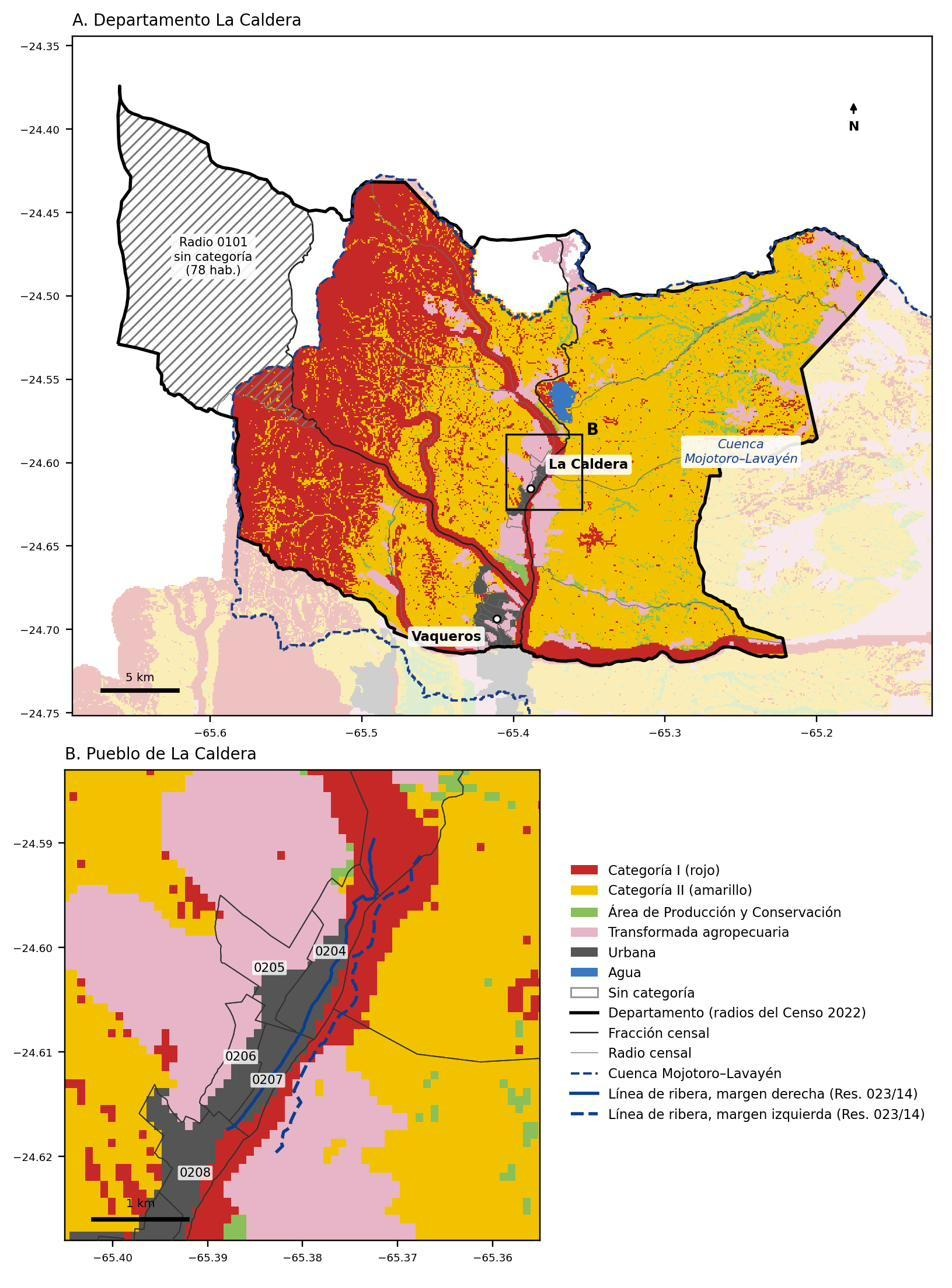
\includegraphics[width=\textwidth,height=0.84\textheight,keepaspectratio]{fig-otbn-cuenca.png}
\caption[El ordenamiento de bosques en el departamento La Caldera]{\textbf{El ordenamiento de bosques en el departamento La Caldera.} A: categorías del mapa final del informe técnico de la Ley 8483 sobre el límite que forman los radios del Censo 2022, con sus fracciones y radios, el límite de la cuenca Mojotoro--Lavayén y, rayado, el radio 0101, que el mapa deja sin categoría. B: el pueblo de La Caldera, con la línea de ribera que la Resolución 023/14 determinó sobre ambas márgenes del río, trazada con sus 134 coordenadas. En blanco, los sectores sin categoría. Elaboración propia con las capas del repositorio del informe técnico (descargadas el 17 de septiembre de 2026), la cartografía de radios del Censo 2022 (INDEC) y las coordenadas del anexo de la Resolución 023/14.}\label{fig:otbn}
\end{figure}

\begin{cautela}
Tres precisiones sobre este cálculo.

\textbf{La capa es la del informe técnico, y reproduce su Tabla 17.} Para la cuenca Mojotoro--Lavayén, el ráster da 56.309 hectáreas rojas, 180.338 amarillas y 29.571 de Área de Producción y Conservación, contra 56.037, 180.784 y 29.744 de la tabla: diferencias menores al uno por ciento, propias del cálculo por píxel. No incorpora los ajustes de la adenda provincial, que filtró polígonos pequeños y sumó bosques del Monte.

\textbf{El resultado no depende del límite.} La superficie censal no coincide con las otras que este libro registra para el departamento (capítulo \ref{cap:fincas}), y ninguna es un deslinde oficial. Tres contornos alternativos dan resultados parecidos: la capa vigente de departamentos del Instituto Geográfico Nacional ---unas 109.200 hectáreas, prácticamente la superficie que el INDEC usa para el censo--- deja el 78 por ciento en la cuenca; el del mismo organismo a escala 1:250.000 ---unas 110.900 hectáreas---, el 75, y el que se arma con las parcelas del catastro rural que acompaña las capas, el 74. Sobre el contorno censal, el de escala 1:250.000 y el catastral, entre el 98 y el 99 por ciento del Área de Producción y Conservación queda dentro de la cuenca. \textit{Sobre la capa vigente del IGN ese último cruce no se hizo: se la incorporó después, cuando el ráster del mapa final ya no estaba entre los materiales procesados, y sólo se midió la proporción de cuenca.}

\textbf{Entre una quinta y una cuarta parte del departamento no tiene categoría.} El mapa deja sin categoría entre 22.400 y 26.800 hectáreas, según el contorno ---el sector noroeste y el que corresponde a la cuenca Grande--Perico, que no figura en la Tabla 17--- porque caen fuera de la capa de cuencas con que se construyó. Con la cartografía censal el sector tiene nombre: 17.700 de esas hectáreas son el \textbf{radio rural 0101 de Vaqueros}, donde el censo contó setenta y ocho habitantes (capítulo \ref{cap:poblacion}), y el resto se reparte entre los radios rurales 0201 y 0202 de la fracción de La Caldera. \textbf{Y con la capa catastral el sector tiene dueño}: unas 19.700 de esas hectáreas son el catastro 102, «Las Nieves», \textbf{tierra fiscal de la Provincia} y territorio que reclama la comunidad kolla Kondorwaira (capítulo \ref{cap:resistencias}, lámina \ref{fig:kondorwaira}). El nuevo artículo 14 de la Ley 7543 pone en Categoría II los inmuebles fiscales con cobertura boscosa; el mapa deja sin ninguna categoría el inmueble fiscal más grande del departamento. Si hay bosque nativo en él y qué régimen lo alcanza, las capas no lo dicen; el apéndice \ref{cap:pedidos} lo pregunta. \textit{Las tres superficies por categoría de este apartado ---28.600, 45.500 y 3.100 hectáreas--- suman 77.200 y, sobre el contorno censal de 107.600, dejarían 30.400 sin clasificar: la diferencia con las hectáreas sin categoría, unas cuatro mil, no se explica con las capas que este libro procesó.}
\end{cautela}

El capítulo \ref{cap:conclusion} vuelve sobre la consecuencia práctica de este cruce: que el desmonte de bosque nativo está vedado en casi todo el departamento.

Dicho lo cual, el efecto que este capítulo describe subsiste, y es lo que hay que sostener con precisión.

La opacidad, aquí, no es un propósito: es una \textbf{consecuencia} del diseño. Un instrumento técnicamente sofisticado, participativo y bien fundado produce, para el ciudadano común, exactamente el mismo resultado práctico que produciría uno opaco: no se puede saber si un bosque determinado es desmontable hasta que alguien presente un proyecto sobre él. El dato no está oculto; \textbf{no existe todavía}.

Y hay un desplazamiento del sujeto que sí conviene registrar. La Resolución 00509 establece que será el titular del inmueble quien identifique dentro del APC la Categoría III sobre la cual se establecerá el proyecto. En el mapa clásico, el Estado decide dónde y el privado consulta. En este esquema, el privado propone dónde y el Estado verifica el cupo. La diferencia no es de legalidad ni de honestidad: es de iniciativa.

De modo que la formulación correcta no es que alguien escondió el mapa. Es que la provincia adoptó un instrumento cuya verificabilidad ciudadana depende enteramente de herramientas informáticas de consulta, y que quien no las domina queda, en los hechos, sin poder responder la pregunta más simple sobre el suelo que tiene enfrente.

\section{Dónde se decide realmente}

La suma de las tres capas produce un desplazamiento que este libro encontró por eliminación.

Los actos políticos visibles que el capítulo \ref{cap:politica} reúne ---el voto del senador contra el ordenamiento de bosques, el Concejo que pide clausurar el ingreso a un loteo y abre el perilago, el municipio que denuncia un loteo ilegal, el intendente que reconoce su insolvencia, el jefe de Gabinete que pide más control--- no son los de un poder capturado.

La decisión que produce el resultado no pasa por los órganos políticos visibles. Pasa por el certificado de aptitud ambiental municipal, por el dictamen del Órgano Técnico de Aplicación y por el expediente de la Secretaría de Ambiente provincial. Tres instancias técnicas, sin votación nominal publicada, sin registro accesible en línea, sin cobertura periodística sistemática y sin obligación de publicar sus fundamentos.

Ése es el mismo hallazgo que \textit{El dispositivo salteño} formuló para la escala provincial: el desplazamiento del órgano político visible al órgano técnico opaco. Que reaparezca en escala municipal, con actores distintos de los que aquel libro estudiaba, es el argumento más fuerte a favor de que se trata de un dispositivo y no de una suma de conductas.

\section{Ocho lugares donde nadie mira}

El apartado anterior estableció dónde se decide. Falta el mecanismo: \textbf{por qué el
resultado se produce sin que nadie tenga que decidirlo}. La respuesta que este libro puede
ofrecer es que el circuito tiene lugares donde la decisión no se toma, no se ve o no se
registra, y que esos lugares no están repartidos al azar.

\begin{cautela}
Lo que sigue es \textbf{inferencia, no documento}. Cada uno de los ocho lugares se apoya en
hechos que este libro documentó y que se citan en su fila; el que los reúne y los presenta como
un conjunto con propiedades comunes es este libro, y ningún expediente lo dice así. El último
apartado enuncia qué hallazgo rompería la construcción, que es la única forma de ofrecerla sin
pedir que se la crea.
\end{cautela}

\begin{ficha}{Ocho lugares donde nadie mira}
\begin{enumerate}[leftmargin=*,nosep]
\item \textbf{El mostrador.} El criterio se aplica sin registrarse. La Zona PU se declara no
urbanizable y el artículo 31 del Código la convierte en trámite de Proyecto Especial; el
proyecto de ordenanza del PDUA deja seis decisiones «a consideración del municipio» sin decir
qué se evalúa, con qué dictamen ni en qué plazo (capítulos \ref{cap:cot} y \ref{cap:pdua}). No
hay expediente del criterio porque el criterio se forma en la atención al público.
\item \textbf{El canal.} La información existe, se publica y no viaja por donde mira el
interesado. La línea de ribera sale dos días en el Boletín y no se asienta en la matrícula
(capítulo \ref{cap:ribera}). El que vende ya lo sabe; el que compra tendría que haber leído el
Boletín de un día determinado de hace once años. \textbf{Y la distinción no es una invención de
este libro}: un auto judicial de 1920, publicado en enero de 1921, ordena publicar un edicto de
deslinde \textbf{treinta días en dos diarios de la capital y «\textit{por una sola vez}» en el
Boletín Oficial} (capítulo \ref{cap:siglo}). El juez separaba, en la misma frase, la publicidad
que da noticia de la que deja constancia.
\item \textbf{El reparto.} Dos organismos intervienen y cada uno supone que el otro miró. La
Resolución 646D/21 registra que Recursos Hídricos intervino a fojas 59 y no dice qué certificó
(capítulo \ref{cap:loteo}). La competencia está dividida; la responsabilidad de mirar, no.
\item \textbf{El espejo.} El que promueve es el que controla: promover, autorizar, evaluar e
inspeccionar la extracción es tarea de una misma oficina (capítulo \ref{cap:amparo}). No hace
falta que nadie se distraiga; no hay quien mire desde afuera.
\item \textbf{El aparato ausente.} La norma presupone un ojo que no existe. Un municipio de
tercera categoría que en 2020 declaró no tener con qué pagar sueldos recibió un Código de
ciento cincuenta y dos artículos diseñado para un cuerpo técnico que no tiene (capítulos
\ref{cap:cot} y \ref{cap:hacienda}). El control está previsto y no está instalado.
\item \textbf{El dato que no se produce.} El parcelario que se ve y no se consulta, el archivo
descargable que se corta en 2015 y el índice que no dice de qué trata nada, todos en este mismo
capítulo. No es información restringida: es información que no se produjo en forma consultable.
\item \textbf{El tiempo.} El acto y su consecuencia quedan separados por más de lo que dura una
gestión ---y a veces el acto llega tarde a su propia fecha: la convocatoria que repone la
elección anulada de 1921 en el distrito de la Caldera se publica \textbf{diecinueve días después
del día que ella misma señalaba para votar} (capítulo \ref{cap:siglo}). La línea de los arroyos El Durazno y Guaranguay se determinó en 2014 y esos arroyos
inundaron el loteo en 2018 (capítulos \ref{cap:ribera} y \ref{cap:amparo}); un trámite de
concesión de agua que lleva nueve años atraviesa dos mandatos completos (capítulo
\ref{cap:redes}).
\item \textbf{La escala.} Se mide el departamento y se decide la parcela. El censo describe
poblaciones, el registro individualiza inmuebles, y ningún organismo tiene por tarea cruzarlos:
los cruces de los capítulos \ref{cap:poblacion} y \ref{cap:ribera} este libro tuvo que hacerlos
a mano.
\end{enumerate}
\end{ficha}

\subsection*{Qué hacen, que es distinto de qué son}

\textbf{Tienen dirección.} Un lugar que ciega a las dos partes por igual se corrige solo,
porque le molesta a alguien con capacidad de reclamar. Éstos ciegan a un lado: al comprador y
no al vendedor, al vecino y no al loteador, al que no tiene abogado y no al que lo tiene. Es lo
que convierte una falla en un sesgo con sentido.

\textbf{No eliminan el costo de averiguar: lo reasignan.} Saber por dónde corre una línea de
ribera cuesta lo mismo en los dos casos. Lo que el lugar ciego decide es quién lo paga.

\textbf{No tienen dueño, y por eso no se reparan.} En cada uno, todos cumplieron: el organismo
publicó, el municipio visó, el registro inscribió lo que le presentaron. No hay funcionario
responsable del hueco porque el hueco está entre dos escritorios. \textbf{Ahí está la inercia}:
el dispositivo no se mantiene, se sostiene solo, y sobrevive a los cambios de gobierno, de
partido y de ley porque ninguno de esos cambios toca el lugar donde está.

\textbf{Cuando se los tapa, se desplazan.} La Ley 8126 obliga desde 2018 a los municipios a
publicar sus ordenanzas en el Boletín y en internet. Vaqueros lo cumple por su cuenta y el
Boletín provincial sigue remitiendo a sus oficinas (capítulo \ref{cap:vaqueros}). El hueco no
se cerró: se mudó de la ordenanza al anexo.

\textbf{Se componen, y ninguno alcanza solo.} Ésa es la razón por la que ningún acto individual
resulta irregular y el resultado se produce igual.

\begin{cautela}
De lo anterior se sigue una consecuencia que corre en los dos sentidos y conviene decirla
entera. Si la suma de estos lugares alcanza para producir el resultado, \textbf{una intención
sería redundante}: no hace falta que nadie lo haya querido. Pero exactamente por eso
\textbf{una intención podría alojarse ahí sin dejar rastro}, porque el dispositivo, por
construcción, no registra lo que pasa en ellos. Este capítulo no puede decidir entre las dos
lecturas, y describir el mecanismo no es un argumento a favor de ninguna.
\end{cautela}

\subsection*{Qué rompería esta construcción}

No se ofrece como interpretación sino como algo que el próximo documento puede quebrar. Tres
pruebas concretas, y ninguna exige acceso extraordinario:

\begin{itemize}[leftmargin=*,nosep]
\item \textbf{El canal se cae} si los informes de dominio muestran que las determinaciones de
línea de ribera posteriores a 2017 sí quedaron asentadas en sus matrículas. Entonces el
problema sería del período y no del circuito.
\item \textbf{El reparto se cae} si la foja 59 del expediente 18-37.348/2019-0 contiene un
certificado con contenido y no una constancia de intervención. Entonces alguien miró, y lo que
hay es un registro incompleto y no un hueco de competencia.
\item \textbf{El conjunto entero se cae} si en las fojas de El Durazno, en los antecedentes
dominiales del corredor o en las respuestas a las cartas de réplica aparece una instrucción o
una gestión dirigida. Entonces no hay ocho lugares donde nadie mira: hay alguien que miró y
decidió, y lo que corresponde explicar es una decisión y no un dispositivo (capítulo
\ref{cap:conclusion}).
\end{itemize}

\section{El parcelario que se ve y no se consulta}

Hay un caso más, y es el único de este capítulo que cualquier lector puede verificar por sí
mismo en cinco minutos, sin pedir nada a nadie.

La provincia mantiene una \textbf{Infraestructura de Datos Espaciales} ---IDESA--- con visor
público en \textit{mapas.salta.gob.ar}. El capítulo \ref{cap:amparo} documenta que el informe de mapas de 2022, incorporado al expediente, declara haberla usado como fuente cartográfica.

Las capas catastrales que el visor atribuye a cada organismo se reproducen en la lámina \ref{lam:idesacat}.

\begin{ficha}{Consulta al visor de IDESA, 15 de septiembre de 2026}
Bajo la categoría \textbf{Infraestructura}, el visor publica la capa \textbf{«Catastro Urbano y
Rural»}, con tres clases activables: \textsc{rural}, \textsc{subrural} y \textsc{urbano}.

\textbf{La capa cubre el departamento La Caldera.} Al acercarse sobre el corredor se dibujan los
polígonos parcelarios: el ejido urbano del pueblo, los fraccionamientos del valle y, al este del
cerro Pucheta, dos conjuntos de parcelas de gran extensión.

Bajo el organismo \textbf{Municipalidad de Salta}, y sólo bajo él, figuran además dos capas
fechadas ---\textbf{«Catastros Sep2025»} y \textbf{«Catastros Jun2026»}---, cada una con
\textbf{«Polígonos Catastro»} y \textbf{«Etiquetas Catastro»}.

\textbf{En el visor no se obtuvieron los atributos de ninguna parcela del departamento}: el
clic devuelve la ubicación ---departamento, municipio, provincia--- y no la matrícula, la
nomenclatura catastral ni la superficie.
\end{ficha}

\begin{cautela}
Hay que decir con precisión qué se observó y qué no.

\textbf{Lo observado} es el comportamiento del visor público en una fecha. No se probó todo el
portal, no se consultaron sus servicios de datos ---que pueden existir y exponer lo que el
visor no muestra--- y no se pidió acceso por ninguna vía formal. Es perfectamente posible que
el dato esté disponible y que este relevamiento no haya sabido llegar a él.

\textbf{Lo que sí queda registrado} es la diferencia entre dos capas del mismo portal: el
catastro de la \textbf{capital} se publica con etiquetas y en dos versiones fechadas; el de los
departamentos se publica \textbf{como dibujo}.

\textbf{Y la consecuencia práctica, que es lo que importa.} Este libro necesitó, capítulo tras
capítulo, saber a qué matrícula corresponde un polígono. Lo pidió a la Dirección General de
Inmuebles ---veintiséis veces, según el apéndice \ref{cap:pedidos}--- porque no encontró
manera de obtenerlo de otro modo. \textbf{El polígono está publicado; lo que lo vuelve útil,
no.}

Es la misma forma que este capítulo viene describiendo, ahora en el instrumento más moderno de
todos: no falta el dato, falta la parte del dato que permitiría usarlo.
\end{cautela}

\lamina{lam-idesa-catastros.jpg}{lam:idesacat}%
{Capas de catastro del visor de IDESA bajo el organismo «Municipalidad de Salta»}%
{\textbf{Panel de capas del visor de la Infraestructura de Datos Espaciales de la provincia},
filtrado por organismo. Bajo \textbf{Municipalidad de Salta} figuran dos conjuntos fechados
---\textbf{«Catastros Sep2025»} y \textbf{«Catastros Jun2026»}---, cada uno con
\textbf{«Polígonos Catastro»} y \textbf{«Etiquetas Catastro»}. La capa provincial «Catastro
Urbano y Rural», que cubre los departamentos, no tiene equivalente etiquetado.}%
{Captura del visor \textit{mapas.salta.gob.ar}, 15 de septiembre de 2026. Se recortó la
porción de mapa para dejar legible el panel; no se alteró ningún tono ni rótulo.}

\subsection*{Lo que la ley manda, y que este capítulo no había leído}

Este capítulo analizó la Ley 8483 por sus efectos cartográficos ---las superficies, el APC, el
área verde--- y no por su articulado. El articulado contiene tres disposiciones que alcanzan
directamente a lo que el resto del libro documenta.

\begin{ficha}{Ley provincial Nº 8483, sancionada el 19 de diciembre de 2024, promulgada por
Decreto 896 del 27 de diciembre --- expediente 91-51.703/24}
\textbf{Artículo 5º}, que sustituye el artículo 20 de la Ley 7543: «\textit{La realización de
\textbf{urbanizaciones}, obras públicas o de infraestructura, prospecciones u obras energéticas
o de vías de transporte \ldots\ en las zonas comprendidas en las Categorías establecidas en el
OTBN y que conlleven un cambio de uso de suelo, serán autorizadas por la autoridad competente
\ldots\ debiendo someterse al procedimiento establecido en el Título III Capítulo VI de la Ley
7070 y \textbf{deberá contar, vista previa mediante, con la no objeción de la Autoridad de
Aplicación} de la presente Ley}».

\textbf{Artículo 3º}: los proyectos de Categoría III «\textit{deberán contar con la
\textbf{consulta libre, previa e informada}, consistente con lo previsto en el artículo 3º
inciso 11) de la Ley 7543 y el \textbf{Convenio OIT Nº 169}, debiendo garantizarse asimismo los
principios de igualdad, publicidad, oralidad, informalidad y \textbf{gratuidad} de la
participación}».

\textbf{Artículo 9º}: la Autoridad de Aplicación, «\textit{en un plazo de \textbf{180 días} a
partir de la promulgación}», deberá «\textit{concluir la \textbf{identificación de los
desmontes ejecutados desde la sanción del primer OTBN e identificar su legalidad}, debiendo
determinar un plan de acción \ldots\ a fin de dar cumplimiento a lo establecido en el artículo
40 de la Ley Nacional 26.331}».

Y el nuevo \textbf{artículo 14}: la Categoría II comprende las áreas «\textit{que poseen una
\textbf{pendiente superior al quince por ciento}}» o suelos con limitaciones severas, e
\textbf{«integran esta categoría los inmuebles fiscales con cobertura boscosa de propiedad de la
provincia»}.
\end{ficha}

\begin{cautela}
\textbf{El artículo 5º es el que más importa, y conviene decir por qué.}

Toda urbanización que implique cambio de uso de suelo en zona categorizada por el OTBN
\textbf{requiere la no objeción de la autoridad forestal}, además del procedimiento ambiental de
la Ley 7070. \textbf{Este libro documenta, en el capítulo \ref{cap:loteo}, urbanizaciones
aprobadas en este corredor, y no tiene la no objeción de ninguna.}

No afirma que falte: la norma es de diciembre de 2024 y varios de esos loteos son anteriores, de
modo que el artículo 7º ---que excluye el efecto retroactivo--- los alcanza. \textbf{Lo que sí
queda establecido es el requisito para lo que venga}, y que el apéndice \ref{cap:pedidos} lo pide desde que
este capítulo lo leyó.

\textbf{El nuevo artículo 14 agrega una segunda pieza.} La Categoría II comprende las áreas de
pendiente superior al quince por ciento ---que es, precisamente, el tipo de ladera sobre la que
la nota de prensa de 2026 sobre las obras de Vialidad Nacional registra emprendimientos privados sin autorización, según el
capítulo \ref{cap:vaqueros}--- \textbf{y los inmuebles fiscales con cobertura boscosa}, que es
lo que el capítulo \ref{cap:tierrafiscal} sigue expediente por expediente.

\textbf{Y el artículo 9º fija un plazo que ya venció.} Promulgada la ley el 27 de diciembre de
2024, los ciento ochenta días se cumplieron a fines de junio de 2025. \textbf{Este libro no sabe
si esa identificación de desmontes y de su legalidad se concluyó, ni si se determinó el plan de
acción.} Es un pedido nuevo y de los que este libro prefiere: un deber con fecha cierta y
vencida.
\end{cautela}

\subsection*{Y el mapa que sí es consultable no está actualizado}

Existe un visor de terceros que publica el ordenamiento de bosques de las provincias en formato
consultable. Sobre Salta, advierte lo siguiente:

\begin{ficha}{Nota del visor, consultada el 16 de septiembre de 2026}
«\textit{El Ordenamiento que se muestra en el mapa \ldots\ corresponde a la Ley \textbf{sin la
actualización del 2025}. Al momento \textbf{no se cuenta con la información en el formato que
permita la actualización} de dicha sección}».
\end{ficha}

\begin{cautela}
\textbf{Es el mismo patrón, en su versión más nítida.} La ley está vigente desde enero de 2025,
su cartografía es el Anexo II, la actualización quedó acreditada por disposición nacional en
octubre de ese año. \textbf{Y quien se dedica a publicar estos mapas dice que no puede
actualizar el suyo porque la información no está en un formato que lo permita.}

\textbf{El informe técnico remite a un repositorio digital con las capas del mapa final y a un Visor desde el que pueden descargarse.} Este libro no sabe si esas capas coinciden con el Anexo II aprobado por la ley. El repositorio sí estaba accesible: de él salen las capas de la lámina \ref{fig:otbn}, descargadas en septiembre de 2026. Y no atribuye a nadie la intención de impedirlo: puede ser una limitación
técnica del visor, o un anexo en PDF, o un trámite que nadie hizo.

\textbf{Lo que registra es el efecto, que es el que este capítulo describe en otros seis
lugares:} la norma se publica, el polígono se aprueba, y lo que permitiría saber qué le toca a
cada parcela no circula en forma utilizable. \textbf{Un tercero que quiere publicarlo no puede.}
\end{cautela}

\subsection*{Aun así, el mapa viejo muestra algo}

Consultado sobre el corredor, ese visor devuelve una imagen legible, con la advertencia puesta
de que corresponde al ordenamiento anterior a 2025.

\begin{ficha}{Categorías de conservación sobre el corredor, según la cartografía previa a 2025}
\textbf{El amarillo ---Categoría II, mediano valor--- cubre prácticamente todo el
departamento}, desde el filo occidental hasta el límite con General Güemes.

\textbf{El rojo ---Categoría I, muy alto valor de conservación--- forma bandas angostas que
siguen los cursos de agua}: una baja por el río La Caldera desde el norte hasta el pueblo y
continúa hacia Vaqueros; otra recorre hacia el este, hacia Campo Santo.

\textbf{El verde ---Categoría III, bajo valor--- aparece en manchones}, concentrados al este del
departamento y en algunos sectores próximos al área urbanizada.
\end{ficha}

\begin{cautela}
\textbf{La coincidencia entre el rojo y los cauces es lo que este libro debe registrar, y sólo
eso.}

\textbf{La categoría de mayor protección del ordenamiento de bosques sigue, sobre este
corredor, las mismas márgenes} donde el capítulo \ref{cap:resistencias} documenta veinte
concesiones de áridos y el capítulo \ref{cap:ribera} reconstruye más de dos décadas de
determinaciones de línea de ribera.

\textbf{No hay contradicción normativa en eso}: la Categoría I protege el bosque, no prohíbe la
extracción de áridos, que se rige por el Código de Minería y tramita ante otra autoridad.
\textbf{Son dos regímenes que recaen sobre el mismo suelo y no se consultan entre sí}, que es lo
que el apéndice \ref{cap:propuestas} propone corregir con un padrón único.

\textbf{Y hay que decir tres veces qué NO prueba esta imagen.} Es la cartografía
\textbf{anterior} a la revisión de 2025, según la advertencia del propio visor. Es una captura
de pantalla \textbf{sin escala gráfica}. Y este libro \textbf{no midió superficies ni verificó
límites}: describe lo que se ve. La categoría de cada sector según el informe técnico ya se calculó con esas capas (lámina \ref{fig:otbn}); lo que sigue pedido en el apéndice \ref{cap:pedidos} es la versión ajustada por la adenda y aprobada como Anexo II.
\end{cautela}

\subsection*{Y dos instrumentos del informe que el libro no había registrado}

El resumen público del informe técnico ---elaborado por el equipo que convocó el Decreto
3749/2014 e integrado por \textbf{Lucas Seghezzo, J.\ N.\ Volante, M.\ A.\ Iribarnegaray, J.\
L.\ Agüero, C.\ Ortega Insaurralde, C.\ D.\ Venencia y A.\ L.\ Zelarayán}--- describe dos
mecanismos que este capítulo no había consignado y que valen para el conjunto del libro.

\begin{ficha}{Umbral de deforestación por cuenca}
«\textit{Las limitaciones a la aprobación de áreas verdes por cuenca se vinculan a la historia
productiva de la cuenca. \textbf{A mayor deforestación pasada, mayores restricciones
futuras}}».

«\textit{\textbf{No se autorizarán proyectos de cambio de uso de suelo en cuencas excedidas en
su umbral máximo de deforestación}, calculado mediante el método del Número de Curva}».

Y sobre el efecto buscado: visibilizar relaciones causales «\textit{podría promover acciones
colectivas a nivel de cuencas para optimizar el uso compartido de la cuenca, por ejemplo,
\textbf{la reactivación de los consorcios de cuencas}}».
\end{ficha}

\textbf{Eso es, en materia de bosques, exactamente lo que este libro propone para el agua.} El
apéndice \ref{cap:propuestas} argumenta que la cuenca del río La Caldera necesita un órgano que
la administre como unidad, y señala que el Código de Aguas tiene consorcios de usuarios pero
ninguno de segundo grado constituido. \textbf{El informe del OTBN llega a la misma conclusión
por otro camino y sobre otro recurso}: la cuenca como unidad de gestión, y los consorcios como
la herramienta a reactivar.

\begin{ficha}{Criterio 11 y protocolo de consulta}
El criterio 11 de la Ley 7.543 ---«\textit{valor y uso dado por comunidades indígenas y
campesinas a áreas boscosas o colindantes}»--- «\textit{será una \textbf{capa de control de
gestión}}», contenida en el \textbf{Mapa 11 del Anexo IX}.

«\textit{Cada proyecto de manejo o cambio de uso del suelo \ldots\ será sometido a un
\textbf{protocolo específico de consulta previa, libre e informada} \ldots\ El proyecto
\textbf{no podrá ser aprobado si no obtiene el visto bueno de las Comisiones de Evaluación}
conformadas para la aplicación del protocolo}» ---Anexo VIII---.
\end{ficha}

\begin{cautela}
\textbf{Esto le da al capítulo \ref{cap:resistencias} un instrumento que no tenía.} Ese capítulo
documenta el relevamiento territorial de la comunidad bajo la Resolución INAI 617/2013 y no
sabe qué efecto jurídico tiene hoy. \textbf{El OTBN revisado le da uno concreto}: si el
territorio relevado está en el Mapa 11, todo proyecto de cambio de uso sobre él requiere
consulta previa y visto bueno de una Comisión de Evaluación.

\textbf{Y lo que el mapa muestra} es una mancha rosa ---«potencial para el uso de comunidades
indígenas»--- que cubre el Valle de Lerma desde el rótulo de La Caldera hasta Coronel Moldes
(Ley 8483, Anexo I, Anexo IX, Mapa 11, pág.\ 87). A la escala del escaneo no se puede saber si
el territorio relevado bajo la Resolución INAI 617/2013 está dentro ni qué superficie del
departamento abarca: el mapa se publica como imagen, sin capa descargable. Sigue pedida la capa
digital.

\textbf{Una precisión sobre esta fuente.} Las citas anteriores salen del \textbf{resumen} del
informe técnico publicado en el repositorio institucional del organismo de ciencia; la lectura
del Mapa 11, del Anexo I completo publicado con la ley. Es una de las pocas \textbf{fuentes académicas con autores identificados} que este libro cita; el apéndice \ref{cap:fuentes} las enumera.
\end{cautela}

\section{La omisión tiene forma}

Los apartados anteriores presentaron casos. Éste los mira juntos y trata a la omisión como lo
que este libro sostiene que es: no un accidente que se repite, sino un objeto con propiedades.
A un objeto así se le pueden hacer seis preguntas ---qué, quién, cómo, de qué forma, cuánto y
cuándo---. Este capítulo contesta las cuatro primeras con documentos y declara por qué no
contesta las dos últimas.

\subsection*{Qué se omite}

Siempre lo mismo, y cabe en una línea: \textbf{se publica la norma de atribución y se reserva
la norma de aplicación}. Lo que falta es o bien el parámetro con el que se decide ---la
superficie mínima, la obra exigible, el puntaje de una discapacidad frente a una familia
numerosa, el plazo para impugnar un padrón, las coordenadas de una línea de ribera--- o bien la
identidad de quien recibe ---la nómina de adjudicatarios, el contrato con sus exenciones---.

La auditoría de pendientes del final de este capítulo llega a lo mismo por otro camino: lo
normativo se consiguió casi todo y lo dominial y societario casi nada. Son dos formas de la
misma frase. \textbf{Se publica la regla y se guardan el número y el nombre.}

\subsection*{Quién omite}

No hay un emisor. En el inventario de este capítulo aparecen los dos municipios, la Secretaría
de Recursos Hídricos, el Poder Ejecutivo provincial y el organismo que administra la tierra
fiscal: dos niveles de gobierno y cinco reparticiones. Eso es, justamente, lo que impide leer
el patrón como una decisión de alguien.

Y hay un segundo actor que conviene separar del primero, porque hasta aquí este libro los trató
juntos y no son lo mismo: \textbf{el que publica no es el que dicta}. La edición web que no
ofrece el enlace «Ver anexo» en ninguno de los instrumentos que quedaron en la lista, el
archivo descargable que se corta en 2015 y el índice que no dice de qué trata nada son
omisiones del publicador, no de los organismos que dictaron los actos. Un acto puede haber
acompañado su anexo y el hueco aparecer igual, aguas abajo. \textbf{Distinguir las dos columnas
---quién dicta y quién publica--- es condición para poder medir cualquiera de las dos.}

\textbf{Y hay una tercera columna, que este libro encontró en un solo caso y que conviene dejar
anotada porque no se parece a las otras dos.} El anexo que la Secretaría de Minería y Energía
remitió al juzgado en junio de 2022 ---los tres cuadros con las veinte concesiones de áridos del
departamento--- está firmado por tres funcionarios de la \textbf{Secretaría de Recursos
Hídricos}, y la nota que lo encabeza \textbf{no lleva firma de nadie} (capítulo
\ref{cap:resistencias}; láminas \ref{lam:notamineria} y \ref{lam:iia}). El que dicta, el que
publica y \textbf{el que certifica} pueden ser tres distintos. Cuando lo son, la pregunta «quién
responde por este dato» no tiene respuesta dentro de la propia pieza. Es una forma de la omisión
que no consiste en no publicar: consiste en publicar sin sujeto.

\subsection*{Cómo se omite: seis mecanismos}

\begin{ficha}{Los seis mecanismos, del más neto al más difuso}
\begin{enumerate}[leftmargin=*,nosep]
\item \textbf{El anexo no acompaña al acto.} La Ordenanza 437 de Vaqueros publica cuatro
artículos aprobatorios y no el Reglamento de Fraccionamiento; los Decretos 3069/14 y 463/15
publican la ratificación y no el contrato; las Resoluciones 142/14 y 236/14 aprueban y
rectifican una determinación de línea de ribera sin publicar las coordenadas, ni las erróneas
ni las corregidas.
\item \textbf{El anexo acompaña, pero no es legible ni buscable.} El de la Resolución 82/16
---la cabeza de la cadena del régimen de tierra fiscal, a la que las demás remiten--- está
publicado como copia certificada de seis folios escaneada sin capa de texto: no aparece en
ninguna búsqueda y hay que abrirlo para saber que está.
\item \textbf{El anexo está publicado en otro lugar, que el acto no indica.} El sexto
instrumento de la lista resultó estar en el digesto del municipio que lo dictó, no donde lo
publicó el acto.
\item \textbf{No hay texto que omitir, porque la decisión se toma caso por caso.} La Zona PU se
declara no urbanizable y el artículo 31 del Código convierte esa prohibición en un trámite de
Proyecto Especial; el proyecto de ordenanza del PDUA deja seis decisiones «a consideración del
municipio» sin decir qué se evalúa, con qué dictamen, en qué plazo ni con qué recurso (capítulo
\ref{cap:pdua}).
\item \textbf{El contenido existe, está identificado y cuesta.} Arancel, horario de atención y
mesa de entradas, que para la mayoría de los vecinos del departamento equivalen a un archivo
cerrado.
\item \textbf{El cambio no deja acto.} Algo que el Estado tenía deja de estar, y ningún acto
publicado lo dispone. El departamento se queda sin Comisión Municipal entre julio de 1921 y abril
de 1922, y el archivo lo sabe sólo porque el decreto que se la devuelve la da a los
departamentos «\textit{que en la actualidad carecen de ella}»; entre 1944 y 1946 hay un
interventor ejerciendo sin decreto de designación publicado; y de los cincuenta y dos nombres con
que doce nóminas oficiales dividieron el departamento entre 1909 y 1940, \textbf{veinticuatro no
están hoy en ningún nomenclador del Estado}, sin acto que los suprima (capítulo
\ref{cap:siglo}, lámina \ref{fig:parajesnom}, y capítulo \ref{cap:ausencias}, más adelante).
\end{enumerate}
\end{ficha}

Los seis van de «no está» a «está y no se encuentra», «está y no donde el acto dice», «no
existe porque nunca se escribió», «existe y se paga» y «pasó y no consta». \textbf{El cuarto es
ausencia de documento en sentido propio}, y es a la vez el más interesante y el menos demostrable: probar
que un criterio nunca se escribió exige haber leído todo lo que podría contenerlo.

\textbf{El sexto es ausencia de acto, no de criterio, y es el más demostrable de los seis},
porque el archivo registra el antes y el después: la comisión que en 1914 repartía un río y la
que en 1922 «carece de ella», los topónimos de las nóminas de 1918 y el nomenclador de 2026. Lo
que no se ve es el acto del medio. \textbf{Y lo que lo revela es casi siempre un acto posterior
que registra el efecto sin nombrar la causa}, que es la misma propiedad que la ficha siguiente
llama el acto que certifica su propio hueco.

\begin{cautela}
Con dos reservas. Que el Estado haya dejado de registrar un topónimo no prueba que el lugar haya
desaparecido: puede seguir vivo en el uso, y este libro no fue a preguntarlo (capítulo
\ref{cap:ausencias}, más adelante). Y que un acto no se haya encontrado vale sólo dentro de los tramos leídos
edición por edición; fuera de ellos, puede existir y no haberse buscado bien.
\end{cautela}

\subsection*{De qué forma: la omisión la declara el acto que la comete}

Ésta es la propiedad que ordena a los demás mecanismos ---al sexto, por un acto posterior---, salvo al cuarto, y conviene enunciarla sola.

\begin{ficha}{Once formas del acto que certifica su propio hueco, y ocho son de hace un siglo}
\begin{itemize}[leftmargin=*,nosep]
\item La Resolución 9/16 remite tres veces al plazo de exhibición de padrones de la Resolución
82/16, dos de ellas a su artículo 5º. El número del que depende toda la arquitectura de control
ciudadano del régimen de tierra fiscal está nombrado, ubicado y no publicado como texto
(capítulo \ref{cap:tierrafiscal}).
\item El Decreto 463/15 lleva al pie la leyenda «\textit{anexo para su consulta en oficinas de
nuestra repartición}». El acto dice dónde está lo que no trae.
\item El edicto de la Resolución 383/14 aprueba la determinación de la línea de ribera en ambas
márgenes de dos arroyos. Una determinación de línea de ribera \textit{es} un conjunto de
coordenadas: el edicto aprueba el conjunto y no lo transcribe.
\item \textbf{Y una forma que 1920 repite tres veces en un año: la vacante sin dueño.} Los tres
decretos que mueven el único puesto rentado de policía de partido del departamento ---el 677, que
acepta una renuncia y no dice quién reemplaza; el 724, que nombra «\textit{para ocupar el puesto
vacante}» sin mencionar la renuncia que el propio Boletín publicó tres semanas antes; y el 901,
que declara la vacante sin nombrar al que la dejó--- \textbf{publican el hueco y no su causa}
(capítulo \ref{cap:siglo}). Y el decreto 1140 del mismo año nombra encargado del Registro Civil
«\textit{con antigüedad al 5 de Agosto ppdo.\ fecha desde la cual presta servicios en carácter de
interino}»: \textbf{el acto reconoce dos meses y medio de ejercicio que nunca se publicaron}.
\item \textbf{Y la forma más pura de todas, que el barrido de 1922 incorporó al cierre: el acto
que declara rectificar otro y no dice qué rectifica.} Un decreto del Poder Ejecutivo provincial,
de junio de 1922, rectifica el artículo 2º del decreto 510 «\textit{en cuanto nombra miembros de
la Comisión Municipal de La Caldera}» y a continuación \textbf{repite los mismos cinco nombres}.
Las únicas diferencias visibles entre el texto rectificado y el rectificatorio son el orden de la
enumeración y una inicial (capítulo \ref{cap:siglo}). \textbf{El acto publica que corrigió y no
publica la corrección}: el lector de 1922 tenía los dos textos delante y no podía saber cuál era
la diferencia.
\item \textbf{Y una segunda de ese mismo año, sobre la pieza que más importa, que ya no es un
caso sino una serie.} El decreto 172 del
15 de julio de 1922 \textbf{aprueba} el presupuesto de gastos y cálculo de recursos que la
Comisión Municipal sancionó el 28 de mayo, previo dictamen del Fiscal General, \textbf{y no lo
transcribe}; \textbf{el decreto 1.975 del 14 de noviembre de 1924 hace exactamente lo mismo},
por remisión al expediente 5162 F y sin una sola cifra, para un ejercicio que terminaba en seis
semanas. En las veintisiete ediciones leídas de 1922 y en las cincuenta y dos de 1924 no hay una
sola cifra de la hacienda del departamento. Catorce y dieciséis años antes, el Boletín había
publicado el cuadro completo de entradas y
salidas del mismo municipio, hasta las sillas de la comisión (capítulo \ref{cap:siglo}).
\textbf{Lo que cambió no fue el acceso: fue qué parte del acto se publica}, y para cuando se
publican los dos decretos de aprobación el cambio ya está hecho.

\textbf{Y la serie tiene un final que conviene decir, porque este capítulo casi nunca registra
desmentidos.} En 1946 el Boletín publica el \textbf{balance del movimiento de la renta} de la
comuna del departamento, cuarto trimestre de 1945, \textbf{con sus renglones y sus saldos
mensuales} ---noventa y ocho pesos con quince centavos al cerrar octubre--- y firma al pie de
cada mes. \textbf{Después de siete actos económicos publicados sin una sola cifra entre 1922 y
1944, se publica el número.} Lo firma un interventor, y es el único balance con cifras de todo
el período. \textbf{La opacidad de esta serie no fue un estado permanente: fue una práctica que
empezó, duró veinticuatro años y se interrumpió}, y eso dice más sobre ella que si hubiera sido
constante.
\item \textbf{Y una cuarta forma, que es la más incómoda porque el hueco lo declara el propio
Estado sobre sus propios registros.} El 1º de julio de 1924 el Ministro de Gobierno resuelve
autorizar al Jefe del Registro Civil a «\textit{investigar el destino que hayan tenido los
libros}» de esa dependencia en el departamento de La Caldera, por tratarse de una medida
«\textit{de naturaleza urgente, dado el hecho que la motiva e intereses que el mismo puede
comprometer}», con cooperación de la comisaría (capítulo \ref{cap:siglo}). \textbf{No dice cuál
es el hecho que la motiva, no dice qué intereses, y no publica el resultado}: ningún acto
posterior del año dice qué encontró la diligencia. \textbf{Es el único caso del archivo temprano
en que lo que puede faltar no es un anexo ni una coordenada sino el registro mismo de los
nacimientos y las muertes de un departamento}, y lo que se publica de eso es que hubo que ir a
buscarlo.
\item \textbf{Y una tercera de la misma especie, en 1923, sobre el acto de mayor alcance del
archivo temprano.} El decreto 1161 del 24 de septiembre declara intervenida la Municipalidad de
La Caldera «\textit{vistas las presentaciones de que instruye el expediente N.\ 4541 F}» y
porque «\textit{los hechos anotados}» en ellas hacen procedente la intervención. \textbf{Ni el
expediente, ni las presentaciones, ni cuáles son esos hechos, ni las instrucciones que el
artículo 2º manda dar al Interventor, ni un solo acto del Interventor se publican} (capítulo
\ref{cap:siglo}). \textbf{Lo publicado permite saber que a este departamento le suspendieron el
gobierno y no por qué.}
\item \textbf{Y una quinta, de 1944, que es la forma más pura de todas: el archivo registra el
efecto y no el acto.} El decreto que aprueba el presupuesto municipal de ese año dice
«\textit{visto este expediente en el que el señor \textbf{Interventor de la comuna de la Caldera}
eleva}» el proyecto de ordenanza. \textbf{Hay un interventor ejerciendo, y ningún acto de los
treinta y dos años leídos dice cuándo se lo designó ni quién es}; la intervención sólo termina en
agosto de 1946, cuando un decreto la da por concluida. \textbf{Se puede saber que el gobierno de
este departamento estuvo intervenido al menos tres años, y no se puede saber desde cuándo}
(capítulo \ref{cap:siglo}).
\item \textbf{Y una sexta, que se ve sólo por contraste, y por eso importa.} En 1944 la refección
del local de la comisaría del pueblo dejó \textbf{licitación, adjudicación, contratista con
nombre, certificado final por \$5.018,02, un adicional y la devolución del depósito en garantía}.
En 1945 las obras de defensa del río de la Caldera se llamaron a licitación pública por
\textbf{\$2.515} y terminaron ejecutándose \textbf{«por vía administrativa»}: \textbf{ni
contratista, ni certificado, ni recepción}. \textbf{Del edificio queda el expediente entero; del
río, sólo la autorización.} No es que falte un documento: es que el mismo Estado, el mismo año y
en el mismo departamento, documenta una obra y no documenta la otra.
\item Y uno de hace un siglo, que el barrido de 1918 incorporó al cierre. Los decretos 113 y
190 de ese año nombran los \textbf{Jueces de Agua} de los distritos de Caldera y Calderilla
«\textit{vista la nota que antecede del Sr.\ Comisionado Municipal de Caldera, proponiendo
\ldots\ las personas}». \textbf{La nota que decide quién administra el agua de los dos
distritos está nombrada, ubicada y no publicada}, y los dos decretos nombran personas distintas
para los mismos dos distritos con seis semanas de diferencia, sin que el segundo cite al primero
(capítulo \ref{cap:siglo}).
\end{itemize}
\end{ficha}

De ahí se siguen dos cosas. La primera es \textbf{lo que vuelve legal a la omisión}: el acto
cumple la publicidad que la ley le exige, y lo que queda afuera queda afuera declaradamente. La
segunda es la que sirve para trabajar: \textbf{el universo de omisiones es cerrado y
enumerable, no estimado}. No hay que inferir el agujero. El agujero trae sus propias
coordenadas, y localizarlo es una operación mecánica sobre el corpus ---buscar los actos que
remiten a contenido que no acompañan---, no un juicio sobre lo que debería estar.

El cuarto mecanismo es la excepción y por eso se lo marca aparte: ahí no hay acto que declare
nada, y todo lo que se diga de él es inferencia.

\subsection*{Las dos columnas que este capítulo no escribe}

\textbf{Cuánto.} El único recuento que este libro tiene es el de su propia lista: tenía trece
instrumentos candidatos y \textbf{ocho salieron al verificarse uno por uno}. De los seis que
quedaron, cinco no se consiguieron. Es decir que \textbf{seis de cada diez de lo que parecía
omisión era falla de recuperación} ---del buscador, del repositorio o de quien buscaba---. Ese
número tiene que gobernar cualquier cuantificación futura, y es la razón por la que esta
columna no se escribe todavía: una tasa de omisión calculada sin descontarlo mide sobre todo la
destreza del que busca.

\textbf{Y dos datos más, reunidos al cierre, empujan en la misma dirección.} El capítulo
\ref{cap:ausencias}, más adelante, daba por ausente del archivo la vida asociativa del departamento, y estaba en
el mismo Boletín, bajo un tipo de aviso que el relevamiento no había mirado. Y este libro afirmó
en tres lugares que la directora jubilada en 1918 era el primer nombre de la escuela del pueblo,
cuando otro de sus capítulos transcribía a la de 1911. \textbf{Ninguno de los dos es un anexo,
pero los dos son ausencias que el libro atribuyó al objeto y eran del que buscaba.}

\textbf{Cuándo.} Los instrumentos del inventario se concentran entre 2014 y 2016, que es
exactamente la ventana que este relevamiento leyó con más intensidad y donde además se
concentran los veinticinco actos de ribera del capítulo \ref{cap:ribera}. \textbf{Mientras el
corpus moderno no esté leído entero, la forma temporal de la omisión es indistinguible de la
forma temporal de la lectura.}

\begin{cautela}
Las dos columnas esperan al corpus completo, y entonces hay tres inflexiones concretas que se
podrán probar y que hoy no. La primera es la línea de base que este mismo capítulo estableció:
los anexos sí se publican, y existe una colección digital separada donde el departamento
aparece con código, importe y expediente. La segunda es la Ley 8126 de 2018, que obliga a los
municipios a publicar sus ordenanzas en el Boletín y en internet: hay que ver si bajó la tasa o
si sólo cambió de lugar. La tercera es el corte del archivo descargable en 2015, que es un
cambio del publicador y no de los organismos, y que por eso debería verse en todos los emisores
a la vez.
\end{cautela}

\subsection*{Lo único que hoy puede decirse del tiempo}

En octubre de 1914 el municipio de La Caldera dictó una ordenanza que repartía la totalidad del
caudal del río Santa Rufina y reconocía derechos adquiridos por uso tradicional. Este libro
leyó las setenta ediciones del Boletín de ese año, una por una, y \textbf{el texto no
está}. En enero de 2015, el municipio de Vaqueros publicó una ordenanza que aprueba en cuatro
artículos un Reglamento de Fraccionamiento de Tierras, y \textbf{el reglamento tampoco está}.

Cien años y un departamento de por medio, la misma figura: \textbf{se conoce que la regla
existe porque otro documento la nombra, y no se conoce la regla}.

\begin{cautela}
Los dos casos no tienen el mismo valor probatorio y no deben leerse como una serie. El de 2015
es una omisión documentada: el acto está publicado, se ve qué publica y se ve qué no. El de
1914 es una ausencia, y una ausencia admite dos explicaciones que este libro no puede separar
---que la ordenanza no se haya publicado en el Boletín provincial, cosa esperable en un acto
municipal de la época; que se haya publicado y no se conserve; o que esté donde este libro
todavía no fue a buscarla, que es lo más probable: las fojas del expediente de 1938 donde el
municipio la invocó, o el libro de actas de la comisión municipal (capítulo
\ref{cap:expropiacion})---. \textbf{Son dos puntos, no una tendencia.} La tendencia, si existe, la dirán las dos columnas que este capítulo dejó sin
escribir.
\end{cautela}

\subsection*{Y dos puntos más, que corren en contra}

Los barridos de 1918 y 1919, incorporados al cierre, agregan algo que este capítulo debe poner
aunque no lo favorezca.

\textbf{El decreto 1.660 del 24 de abril de 1918 publica su propia cuenta.} Es el acto que
devuelve a La Caldera la condición de Comisión Municipal, después de que el decreto 1.557 la
hubiera convertido en Municipalidad electiva siete semanas antes, y para fundarlo el Boletín
imprime las tres cifras: el cálculo de recursos de \textbf{\$6.471,44}, el saldo del ejercicio
anterior indebidamente computado, \textbf{\$3.083,94}, y la renta real resultante,
\textbf{\$3.387,50}, contra el mínimo de cinco mil que la norma exigía (capítulo
\ref{cap:siglo}).

\begin{cautela}
\textbf{Es exactamente lo contrario de lo que este capítulo describe para 2014--2026.} Ahí el
acto publica la atribución y reserva el parámetro; acá el acto publica el parámetro, el umbral,
la cuenta y el resultado, en el mismo renglón en que decide. Un vecino de 1918 que abriera el
Boletín podía saber por qué su departamento no se gobernaba a sí mismo, y por cuánto. Un vecino
de 2015 que abriera el Boletín no podía saber qué obras le eran exigibles al loteador de
enfrente.

\textbf{Y no es un caso aislado: el año siguiente lo repite otro gobierno.} El decreto 33 del 15
de enero de 1919, que nombra la Comisión Municipal del departamento, publica el criterio entero
en su considerando ---qué artículo de la Ley Orgánica se invoca, qué artículo de la Constitución
lo derogó, y cuál es el umbral: «\textit{un centro urbano de cinco mil habitantes, de que carecen
todos los Departamentos de Campaña}»--- y hasta declara el programa de gobierno que lo
enmarca (capítulo \ref{cap:siglo}). \textbf{Dos actos, doce meses, dos gobiernos distintos, y
los dos publican la regla con la que deciden}: uno el número, el otro la norma.

\textbf{Dos casos tampoco son una serie}, y conviene decir con qué se los puede tumbar: bastaría
con un acto de la misma época que reserve su criterio para que el contraste se disuelva. \textbf{Y
este mismo capítulo tiene uno}: el decreto 1161 de 1923, que interviene el municipio por «\textit{los
hechos anotados}» en un expediente que no se publica, es de cinco años después y decide sobre lo
mismo ---quién gobierna el departamento---. De modo que el contraste no separa dos épocas: \textbf{en
1918 y 1919 el Estado publicó la regla con la que decidía la condición institucional del
departamento, y en 1923 decidió lo mismo sin publicarla}. Este libro, además, no leyó de corrido
el segundo semestre de 1922 ni nada entre 1947 y 2012 ---1947 a 1950 se barrieron sin lectura
sobre la imagen---, de modo que \textbf{la afirmación fuerte ---que la opacidad de criterio es algo que
apareció y no una constante del Estado provincial--- sigue sin poder hacerse}. Lo que sí queda
establecido es que no siempre fue así, y que hay dos actos fechados que lo prueban.
\end{cautela}

\subsection*{Y una omisión de 1919 que no es de criterio sino de sujeto}

Hay en 1919 una forma que este capítulo no tenía y que conviene anotar, porque no consiste en
reservar un contenido sino en publicar mal quién decide.

\textbf{La mancheta de las cuarenta y nueve ediciones del año atribuye el gobierno al Dr.\
Joaquín Castellanos.} Y sin embargo el Ejecutivo lo ejerce el \textbf{Presidente del Senado} en
treinta y dos de ellas, en dos interinatos separados por un regreso del titular, \textbf{sin que
se publique un solo decreto de apertura ni de cierre de ninguno de los dos} (capítulo
\ref{cap:siglo}).

\begin{cautela}
\textbf{El envoltorio dice una cosa y la firma dice otra, en la misma hoja.} Quien lea la tapa
sabe quién gobierna; quien lea el pie del decreto sabe quién firmó; y nadie puede saber desde
cuándo ni hasta cuándo, porque el acto que lo dispone no se publica.

Es la misma estructura que este capítulo describe, corrida un lugar: no falta el criterio, falta
\textbf{la constancia de quién estaba habilitado para aplicarlo}. Y se parece a lo que el
apartado anterior llama la tercera columna: el que dicta, el que publica y el que certifica
pueden no coincidir, y aquí no coinciden ni siquiera el que gobierna en la tapa y el que firma
adentro.
\end{cautela}

\section{El límite de lo que se puede afirmar}

Corresponde ahora la parte más incómoda, y va sin atenuantes.

Todo lo que este libro documentó tiene una explicación estructural completa y suficiente. Un municipio clasificado en tercera categoría, que en 2020 declaró no tener con qué pagar sueldos, recibió en 2015 un plan urbano y en 2016 un Código de ciento cincuenta y dos artículos diseñado para un aparato técnico que no posee, y absorbió entre 2010 y 2022 el cuarto crecimiento poblacional de la Argentina. La Provincia y el Consejo Federal de Inversiones financiaron la redacción de la norma; nadie financió la estructura que debía aplicarla. El mercado ocupó el espacio que esa incapacidad dejó libre.

Esa explicación no requiere que nadie haya decidido producir el resultado.

\begin{cautela}
Pero la explicación estructural es también, exactamente, lo que un dispositivo produciría si funcionara bien.

Este libro no puede distinguir, con los documentos que consiguió, entre un Estado desbordado y un Estado desbordado que a alguien le conviene que siga desbordado. Los dos se ven igual desde afuera. Un municipio sin capacidad técnica y un municipio al que no se le da capacidad técnica producen el mismo expediente vacío.

Distinguirlos requeriría lo que no está en ningún archivo: saber qué se conversa en las oficinas donde la excepción se tramita. Ese es el límite de una investigación documental, y el libro llega hasta ahí y se detiene.

Lo que en efecto puede afirmarse sin ambigüedad es que la opacidad de este departamento no es un secreto guardado. Es una capa fina y enteramente legal, hecha de anexos no publicados, de excepciones que se tramitan y de actos individuales que nunca se registran públicamente, y basta para que nadie pueda reconstruir una decisión sin ir físicamente a una oficina. Es más eficaz que cualquier ocultamiento, porque no deja nada que denunciar.
\end{cautela}

\section{Las tres cosas que quedaron sin resolver}

No son misterios. Son trámites, y su resolución no depende de encontrar nada oculto.

\textbf{Primero.} Si la actual titular del organismo provincial que administra la tierra fiscal es copropietaria de un loteo cerrado en el departamento que representó ocho años en la Legislatura. Se resuelve con el informe de dominio de una matrícula.

\textbf{Segundo.} Cuándo, a instancia de quién y por qué motivo la sociedad titular del loteo El Durazno fue incorporada como tercero al amparo colectivo que litiga por la inundación de ese loteo. Se resuelve con el expediente completo.

\textbf{Tercero.} Si veintiséis de los treinta adjudicatarios del barrio Juan Manuel de Rosas son vecinos de La Caldera, como sostuvo el centro vecinal. Se resuelve con el domicilio de los adjudicatarios, que ninguna de las dos versiones del anexo consigna.

Las tres se responden con documentos que existen y a los que este relevamiento no accedió. Que sigan sin respuesta no es prueba de nada: es la medida exacta de hasta dónde llegó este trabajo.

\section{La forma del hueco}

Al cerrar el libro se auditaron uno por uno los marcadores de pendiente que quedaron en el texto, para establecer cuáles podían resolverse en fuentes abiertas y cuáles no. El resultado de esa auditoría es, en sí mismo, un dato sobre el objeto, y por eso se consigna aquí y no en un apéndice de método.

Lo que se pudo cerrar es casi todo normativo. Se obtuvieron el texto de la ley orgánica de municipalidades, el de la ley de áreas protegidas, la secuencia completa del régimen nacional de expansión de redes de gas, la identificación de la ley general de expropiaciones, el contenido resolutivo de la última audiencia del amparo y la ubicación exacta de la desagregación censal por municipio.

Lo que resistió es casi todo dominial y societario. Ningún antecedente de finca, ningún informe de dominio, ningún legajo de sociedad; de los expedientes judiciales, piezas del incidente y de la ejecución ---providencias, actas e informes--- pero no la sentencia ni el expediente principal; y el único plano de mensura obtenido ---el 000962--- llegó como anexo de un decreto.

\textbf{Esa asimetría no es un accidente del método de búsqueda: es la arquitectura de acceso del sistema.} Toda la información que permite saber cuánta gente vive en el departamento y en qué condiciones es gratuita, remota y descargable. Toda la información que permite saber quién es dueño de qué es arancelada, presencial y, en algunos casos, requiere acreditar interés legítimo.

\textbf{Y lo dominial no le resiste sólo al vecino: también le resistía al Estado.} En 1939 la Curia promovió posesión treintañal (capítulo \ref{cap:fincas}); en 1943 la Provincia tuvo que promover juicio de posesión treintañal para titular el terreno donde su propia comisaría funcionaba desde 1913 o antes (capítulo \ref{cap:presencia}); y en 2015 adquirió por prescripción el suelo de la escuela de El Gallinato, que funcionaba en terreno ajeno desde 1968 (capítulo \ref{cap:tierrafiscal}). Entre 1939 y 2015, tres ocupantes institucionales tuvieron que titular por prescripción lo que ya usaban. \textbf{El registro de la propiedad no es opaco sólo para quien pregunta desde afuera: tampoco le alcanzaba al Estado para saber qué era suyo.}

\textbf{Y la asimetría tiene una medida exacta en un solo año.} En 1920 el Boletín publica \textbf{diez resúmenes del movimiento de la Tesorería General}, uno por mes y encadenados por la existencia de caja, y \textbf{ningún balance municipal}: ni de este departamento ni de ningún otro (capítulo \ref{cap:siglo}). Diez a cero, en el mismo boletín y en el mismo año. El Estado provincial rinde su caja mes a mes; los municipios, que son los que deciden sobre el suelo, no rinden ninguna, y el capítulo \ref{cap:hacienda} muestra que un siglo después la información fiscal municipal sigue siendo lo más difícil de conseguir de este territorio.

Un Estado que publica generosamente las reglas y resguarda los nombres no está ocultando nada: está distribuyendo el costo de averiguar. Y ese costo lo paga entero quien quiera reconstruir la propiedad del suelo, mientras no lo paga nadie que quiera describir la pobreza.

Es la misma capa fina que este capítulo viene describiendo, vista desde el otro lado. No hay un archivo cerrado. Hay un arancel, un horario de atención y una mesa de entradas, que para la mayoría de los vecinos del departamento equivalen a un archivo cerrado.

\subsection*{Lo que el Estado sí declara de interés}

Una nota breve, y no es ironía.

El 13 de noviembre de 2015, por \textbf{Decreto Nº 3760}, el Poder Ejecutivo declaró de \textbf{Interés Provincial la Fiesta Patronal de Nuestra Señora de la Candelaria} de la localidad de La Caldera, a celebrarse el 2 de febrero de 2016.

Se consigna porque forma parte del registro y porque contradice, en su pequeñez, una lectura fácil de este libro.

El Estado provincial no ignora a La Caldera. La nombra, la visita, declara de interés su fiesta patronal, contrata a su municipio para mantener rutas, le construye aulas, le cede el arancel de las licencias de conducir, sostiene allí centros de mediación comunitaria. La relación es densa y continua.

Lo que este libro describe no es abandono. Es \textbf{selectividad}: un Estado muy presente en algunas dimensiones --- la turística, la vial, la ceremonial --- y sistemáticamente tardío en otras --- el agua de red, la cloaca, el control del fraccionamiento, la publicación de las coordenadas ---. Confundir las dos cosas sería un error de diagnóstico, y de él se sigue un error de reclamo: no se le pide a este Estado que llegue, se le pide que llegue con lo otro.

\subsection*{El río como frontera de la notificación}

Hay una pieza de 1975 que sigue rigiendo y que conviene poner junto a las demás.

\begin{ficha}{Acordada Nº 4529/75 de la Corte de Justicia, citada en el B.O.\ Nº 19.256 de 2014}
La zona en la que la oficina de Ujiería del Poder Judicial realiza las diligencias de notificación está comprendida dentro de estos límites: ``\textbf{Norte: Río Vaqueros}; Sur: Río Ancho; Este: kilómetro 5 de la Ruta Nacional 34; Oeste: río San Lorenzo''.
\end{ficha}

El río Vaqueros vuelve a aparecer como límite, y esta vez no de una competencia municipal sino de la notificación judicial.

Al norte de ese río --- es decir, en Vaqueros y en La Caldera --- las diligencias no las hace la ujiería. Quien litiga desde el departamento debe constituir domicilio \textbf{dentro} del radio, en la capital, y si no lo hace las notificaciones se tienen por practicadas por ministerio de la ley: corren los plazos aunque no se haya enterado.

No es una norma dirigida contra el departamento. Es un radio de ujiería trazado en 1975 sobre accidentes geográficos, cuando al norte del río Vaqueros vivía una fracción de la población actual. Hoy viven doce mil trescientas personas.

Pero el efecto acumulado es el que este capítulo describe. El vecino que quiere apelar una línea de ribera tiene diez días hábiles y las coordenadas en una sede de la capital. El que quiere consultar un plano paga arancel y va presencialmente. El que litiga debe constituir domicilio en la ciudad o asumir que los plazos corren sin él. Ninguna de esas tres reglas fue escrita para excluir a nadie. Las tres tienen el mismo efecto, y las tres se apoyan en la misma premisa tácita: que el interesado está del otro lado del río.

\subsection*{Y a veces no hay nada}

Conviene registrar también el reverso, porque el relevamiento sistemático del Boletín Oficial permite medirlo.

Entre el 11 de junio y el 3 de julio de 2014 --- quince ediciones, quinientas cuarenta y dos páginas --- el departamento La Caldera aparece \textbf{una sola vez}, y es el mismo aviso repetido cinco días por mandato legal: la solicitud de un particular para extraer agua de un pozo. Ni Vaqueros, ni La Calderilla, ni Yacones, ni Lesser figuran en todo el período.

No hay que forzar la lectura. Tres semanas sin actos referidos a un departamento que entonces tenía unos nueve mil habitantes es lo normal en el boletín de una provincia de alrededor de un millón trescientos mil, y la ausencia de noticias no significa ausencia de gestión: significa que los actos que la administración publica --- decretos, licitaciones, edictos --- se producen a un ritmo irregular.

Y el fenómeno se repite y se puede medir mejor. Entre el 10 de noviembre y el 2 de diciembre de 2014 --- dieciséis ediciones, seiscientas veinticuatro páginas --- la expresión ``La Caldera'' \textbf{no aparece una sola vez}. Tampoco ``La Calderilla'', ni ``Yacones'', ni ``río Caldera''. El relevamiento que arroja ese resultado validó la capa de texto de los archivos corriendo reconocimiento óptico propio sobre una muestra y comparando volúmenes de caracteres, y corrió además una búsqueda difusa tolerante a los errores típicos de escaneo: los seis aciertos fueron falsos positivos --- ``escalera comunitaria'', ``zona tabacalera del Río Toro'', ``calle Rafael Obligado''. \textbf{El cero es real, no un artefacto de extracción.} Es, con todo, un cero del término y no del departamento: en esa misma ventana el Boletín Nº 19.430, del 19 de noviembre, publica la convocatoria a asamblea de la asociación vecinal de los ríos Castellanos y Lesser (capítulo \ref{cap:resistencias}).

Lo que puede decirse, y es modesto, es que \textbf{la presencia del departamento en el registro oficial es intermitente y desigual}. Se concentra en rachas --- veinticinco actos hídricos en dos años, seis concesiones de áridos en dos --- y desaparece por semanas enteras, con actos sueltos fuera de las rachas, como la línea de ribera del río Wierna de noviembre de 2016, cuyas coordenadas tampoco se publicaron. Quien quiera reconstruir la vida administrativa del corredor leyendo el Boletín no encontrará una serie continua sino un pulso: períodos densos separados por vacíos.

Eso importa para el método de este libro más que para su tesis. Explica por qué la reconstrucción documental produce imágenes nítidas de algunos años y ninguna de otros, y por qué el silencio de un período no autoriza a concluir que en ese período no pasó nada.

\subsection*{El archivo descargable se corta en 2015}

Este libro se construyó, en buena parte, descargando ediciones completas del Boletín Oficial y leyéndolas. Ese método tiene un límite y conviene dejarlo escrito, porque no es una limitación del trabajo sino del repositorio.

\begin{ficha}{Comprobación del 7 de septiembre de 2026}
El sitio del Boletín Oficial de Salta publica sus ediciones en formato descargable bajo una dirección predecible, del tipo \texttt{/pdfs/<año>/<número de edición>.pdf}.

Probadas cinco ediciones espaciadas de cada año entre 2005 y 2026, el resultado es inequívoco: \textbf{todos los años de 2005 a 2015 responden; todos los de 2016 a 2026 devuelven error 404}. No es un bloqueo por exceso de pedidos --- eso daría otro código --- sino ausencia de los archivos en esa ruta.
\end{ficha}

\begin{cautela}
De modo que la última década del Boletín Oficial \textbf{no se puede descargar en bloque}. Se consulta de a un acto por vez, a través de la interfaz del sitio, y para llegar a un acto hay que saber de antemano su número o su fecha.

Esto no es una denuncia y no debe leerse como tal. Puede obedecer a una migración de plataforma, a una decisión de almacenamiento o a una política de acceso deliberada y perfectamente legítima. Este libro no sabe cuál de las tres, y no lo averiguó.

Lo que corresponde registrar es el \textbf{efecto}, que es idéntico al de los otros casos de este capítulo. La información está publicada: cualquiera puede leer el Boletín de 2019 acto por acto. Lo que no puede es \textbf{leerlo entero}, ni buscar dentro de él, ni preguntarle cuántas veces aparece un topónimo, una empresa o una matrícula. Y esas son, exactamente, las preguntas que permiten reconstruir un dispositivo.

El resultado práctico es una asimetría curiosa: \textbf{los años más antiguos son los más accesibles}. Este libro pudo reconstruir con detalle el ciclo hídrico de 2013 a 2015 --- veinticinco actos, más de veinticinco inmuebles, trece cursos --- y no puede hacer lo mismo con el período que va del primer aluvión a la sentencia. Para 2018 y 2019, los años decisivos de esta historia, la reconstrucción documental depende de conocer de antemano qué buscar.

Quien quiera contar lo que pasó en el corredor entre 2016 y 2026 deberá pedirlo pieza por pieza, y sólo encontrará lo que ya sospechaba.
\end{cautela}

\subsection*{Un índice que no dice de qué trata nada}

Hay un caso que conviene mostrar entero, porque es pequeño, es verificable y explica la arquitectura mejor que cualquier generalización.

El Boletín Oficial de Salta publica en línea sus \textbf{índices de decretos} por año, desde 1983. Se descargan sin arancel, sin trámite y sin identificarse. Es, en apariencia, transparencia retrospectiva completa.

\begin{ficha}{Índice de Decretos, año 1983 --- estructura}
El documento tiene sesenta y siete páginas y tres columnas: \textbf{número de decreto}, \textbf{fecha de publicación} y \textbf{número de edición} del Boletín. Enumera 2.176 decretos, y a partir del 19 de diciembre de 1983 ---así en el índice; el cambio de gobierno fue el 10--- la numeración vuelve a empezar en 1.

No consigna materia, organismo, beneficiario ni objeto. Muchas filas ni siquiera tienen fecha: sólo el número.
\end{ficha}

\begin{cautela}
Léase lo que eso significa para cualquiera que busque algo.

Este libro necesita, para el capítulo \ref{cap:politica}, los decretos por los cuales se designaron los titulares del ejecutivo municipal de La Caldera entre 1983 y 1987 --- presidentes de Comisión Municipal que no se elegían sino que los nombraba el gobernador. El índice permite saber que en 1983 hubo 2.176 decretos y en qué edición del Boletín salió cada uno. \textbf{No permite saber de qué trata ninguno.}

Encontrar uno exige abrir las ediciones del Boletín y leerlas. Para un solo año, eso son más de doscientas cincuenta ediciones. Para el período completo, cuatro veces eso.

El dato no es que la información esté oculta: \textbf{está publicada}. El dato es que está publicada de una manera que sólo sirve a quien ya sabe el número del decreto que busca --- es decir, a quien no necesita el índice. Un índice sin materia no es un índice: es una lista.

Y ésa es, en miniatura, la forma completa del problema que este capítulo describe. La opacidad de este dispositivo casi nunca consiste en negar un documento. Consiste en entregarlo de un modo que preserva su inaccesibilidad práctica: el anexo que no acompaña al acto, las coordenadas que quedan en la sede, el plano que se consulta con arancel, el índice que no dice de qué trata nada.
\end{cautela}

\parte{Cierre}
{Qué quedó probado, qué no, y qué falta para probarlo.}
\chapter{El departamento que no está en los expedientes}
\label{cap:ausencias}

Este libro tiene veintiocho capítulos sobre un lugar donde viven doce mil trescientas personas,
y las personas casi no aparecen.

Aparecen como firmantes de resoluciones, como partes de un remate, como titulares de una
matrícula, como damnificados de un aluvión que otro relevamiento entrevistó. No aparecen
comprando, estudiando, enfermándose, yéndose ni quedándose. \textbf{El apéndice \ref{cap:fuentes} lo advierte: el departamento aparece tal como el Estado lo escribió. Este capítulo hace el
inventario de lo que esa elección dejó afuera.}

No es un capítulo de conclusiones. Es un mapa de huecos, con lo poco que el archivo sí dejó de
cada uno, y con lo que haría falta para llenarlos. Sirve para que un lector sepa qué no está
leyendo, y para que quien continúe este trabajo no empiece de cero.

\section{Por qué faltan}

La razón no es una omisión del autor: es una propiedad del archivo.

\textbf{Los expedientes registran la propiedad y el agua porque de eso se ocupan.} Un remate
deja constancia de quién compró y en cuánto, no de quién trabajaba esa tierra. Una determinación
de línea de ribera fija coordenadas, no cuántas casas quedan adentro. Un decreto de promoción
turística consigna un beneficiario, no cuántos puestos de trabajo generó ---y el capítulo
\ref{cap:trabajo} muestra que nadie está obligado a informarlo---.

\textbf{De modo que la ausencia también es un dato.} Un territorio del que el Estado guarda
tres siglos de títulos y casi ningún registro de vida cotidiana está diciendo algo sobre qué
consideró digno de registro.

\begin{cautela}
Con una salvedad que hay que hacer, porque si no este capítulo se vuelve una queja.

\textbf{Los registros de la vida cotidiana existen y no están en los archivos que este libro
consultó.} Hay legajos escolares, historias clínicas, libros parroquiales, padrones de
comercios, expedientes de la comisaría. No están en el Boletín Oficial ni en la Dirección
General de Inmuebles, y varios ---con razón--- no son públicos.

Lo que falta, entonces, no es que el Estado no registre la vida. Es que \textbf{este
relevamiento eligió un archivo y ese archivo no la contiene}.
\end{cautela}

\section{Lo que sí quedó, por dimensión}

\subsection*{Los nombres que se borraron}

Hay una ausencia que este capítulo puede medir, y es nueva. El capítulo \ref{cap:siglo} reúne las
doce nóminas con que el Estado provincial nombró las unidades de este departamento entre 1909 y
1940 ---policía, Código Rural, circuitos electorales--- y las cruza con los dos nomencladores
vigentes: el campo «finca» del catastro parcelario y la Base de Asentamientos Humanos.

\textbf{Veinticuatro de los cincuenta y dos nombres no están en ninguno de los dos} (lámina
\ref{fig:parajesnom}). Siete de ellos son lugares donde el circuito electoral de 1918 declara que
vive gente que vota ---Despensilla, Corral de Barrancas, El Churcal, El Monte, Las Garrapatas, El
Túnel y La Despensa---, y otros los registraban todavía los circuitos de 1921 y el padrón de 1940: El
Bordo, la Estación del ferrocarril, Severino, Los Chusos, Higueritas, Los Matos, Nogalito y La
Sierra.

\begin{cautela}
\textbf{No se afirma que esos lugares hayan desaparecido.} Un topónimo puede seguir vivo en el uso
y no estar en un nomenclador, y este libro no fue al territorio a preguntarlo ---que es,
exactamente, la carencia que este capítulo inventaría---. Lo que queda establecido es más chico y
se puede verificar: \textbf{el Estado dejó de registrarlos, y no hay acto que lo disponga}. Se
borraron entre dos formularios.
\end{cautela}

\subsection*{La escuela}

Es la dimensión con más huellas, y son huellas indirectas: las escuelas aparecen porque tienen
inmuebles.

El capítulo \ref{cap:tierrafiscal} documenta la \textbf{Escuela Nº 4118 «Dr.\ Gustavo Martínez
Zuviría»}, del paraje El Gallinato, que funciona desde 1968 en un terreno ajeno y cuyo suelo la
Provincia adquirió por prescripción en 2015. \textbf{Y hay dos nombres entre los que este libro transcribe del archivo temprano, y los dos aparecen por jubilarse, no por enseñar}: en julio de 1911 el Ministerio de Hacienda jubila a \textbf{Jacoba Luquez de Gómez, directora de la escuela elemental de la parroquia} (capítulo \ref{cap:presencia}), y el decreto 1.653 del 20 de abril de 1918 jubila a \textbf{Juana Luque, Directora de la Escuela de la Caldera}, con ciento cuatro pesos cincuenta centavos mensuales (capítulo \ref{cap:siglo}). La semejanza de los apellidos no autoriza a identificarlas entre sí ni a suponer parentesco: son dos actos distintos, con siete años de distancia. Una versión anterior de este párrafo decía que el nombre de 1918 era el único; el propio libro transcribía el de 1911. El recuento vale sobre lo que el libro transcribe y no sobre el archivo: los tramos leídos después de los primeros no se repasaron buscando nombres de docentes. Aparecen además la \textbf{Escuela Nº 136 Juana
Moro de López}, la \textbf{Escuela Nº 660 de Finca Mojotoro}, la \textbf{Escuela Nº 4534 de Los Yacones} y el \textbf{Colegio Nº 5045 «Senado Provincial»}.

\textbf{Lo que no se sabe:} cuántos alumnos, cuántos establecimientos hay en total, qué
proporción termina la primaria y dónde cursan la secundaria quienes la terminan. Y algo que el
capítulo \ref{cap:poblacion} vuelve pertinente: si los chicos del corredor van a la escuela del
departamento o viajan a la capital.

\subsection*{La salud}

Es el hueco más grande del libro. Lo que hay es histórico y escaso: un lazareto improvisado
durante la viruela de 1908 (capítulo \ref{cap:siglo}), una estación sanitaria prometida en 1935
que no dejó rastro y un guarda sanitario a sueldo provincial (capítulo \ref{cap:presencia}), y
una deuda del municipio con Sanidad en 1940 (capítulo \ref{cap:hacienda}). \textbf{Del presente,
nada.}

No se sabe cuántos centros de salud hay, con qué horarios, con qué personal, ni a dónde va
alguien que necesita atención de urgencia a las tres de la mañana en un departamento a veinte
kilómetros de la capital. Tampoco si el crecimiento poblacional que el capítulo
\ref{cap:poblacion} documenta tuvo correlato en infraestructura sanitaria.

\subsection*{El comercio y el abastecimiento}

Siete menciones, todas de paso.

No se sabe dónde se compra la comida, cuántos comercios hay, si existe feria, ni qué proporción
del consumo se hace en la capital. En un departamento cuya superficie agropecuaria declarada cayó un ochenta y ocho por ciento ---capítulo \ref{cap:tierra}---, saber de dónde viene hoy la comida
no es un detalle costumbrista.

\subsection*{El transporte}

Acá el archivo dejó algo mejor, y por una vía inesperada.

El capítulo \ref{cap:resistencias} documenta que \textbf{Transporte Hnos.\ Mendoza S.R.L.}
tramitó ante el Juzgado de Minas la renovación de la concesión de la cantera de áridos
«Macarena». \textbf{La misma razón social aparece como transportista y como concesionaria de
extracción sobre el cauce.} El capítulo \ref{cap:redes} documenta además la creación de una
autoridad metropolitana de transporte, que el capítulo \ref{cap:aguabaja} señala como la única
figura de coordinación que la provincia construyó para este corredor.

\textbf{Lo que no se sabe:} qué servicios de pasajeros existen hoy, con qué frecuencia y a qué
costo, y si alcanzan a los parajes o solo al casco urbano.

\subsection*{Los jóvenes y la migración}

El capítulo \ref{cap:resistencias} registra, tomándolo del libro de la
comunidad, el \textbf{despoblamiento del cerro y la migración de los jóvenes}. Y el capítulo
\ref{cap:tierra} documenta el movimiento inverso y anterior: la llegada de trabajadores del
tabaco desde el interior provincial y desde Bolivia, primero golondrinas y después radicados.

\textbf{Dos migraciones en direcciones opuestas, separadas por décadas, y de ninguna se sabe
cuánta gente movió.}

\subsection*{La vida asociativa}

Es la dimensión mejor conservada, porque las asociaciones sacan personería y las personerías se
publican.

El capítulo \ref{cap:resistencias} reúne al menos siete asociaciones civiles con personería en el departamento; de varias, este libro no pudo establecer la continuidad después de 2015.

\textbf{Y acá el hueco se llenó mientras este capítulo se escribía}, porque las asambleas de
entidades civiles se publican en el Boletín Oficial y forman una serie.

\begin{ficha}{Entidades del departamento con asamblea publicada, 2016--2026}
\textbf{Clubes:} Social y Deportivo de Caza y Pesca La Caldera; Deportivo Jardín; Social y
Deportivo San Roque; Deportivo La Verbena; Social y Deportivo La Caldera; Social, Cultural y
Deportivo Sportivo Vaqueros; Club Nuevo Horizonte.

\textbf{Jubilados y cultura:} Centro de Jubilados y Pensionados Cristo Monumental, con
asambleas en 2017, 2018, 2019, 2021, 2022, 2023, 2024 y 2025; Biblioteca Popular Roberto
Romero, de Vaqueros, con serie igual de continua; Centro Gaucho El Palenque.

\textbf{Emergencias:} Asociación de Bomberos Voluntarios 2 de Junio, Vaqueros; y Asociación
Civil Papa Francisco, Bomberos Voluntarios de La Caldera, con asamblea en 2026 ---y, en marzo de ese año, intervenida: la Inspección General de Personas Jurídicas encontró su sede cerrada y abandonada, declaró la caducidad de los mandatos de su comisión directiva y nombró interventoras (Resolución 26/26, B.O.\ Nº 22.162; capítulo \ref{cap:amparo}). Fundada en septiembre de 2013 según el registro del Sistema Nacional de Bomberos Voluntarios, con personería de 2016; su cuartel está en la avenida Costanera, en su cruce con la avenida San Martín, en el pueblo de La Caldera---.

\textbf{Producción y trabajo:} Asociación de Pequeños Productores Agropecuarios; Cooperativa de
Trabajo Salta Norte 3 Ltda.; \textbf{Cámara de Turismo del Departamento La Caldera}.

\textbf{Vecinales y urbanizaciones:} Centro Vecinal Barrio El Durazno; Club de Campo Vertientes
Eco-Pueblo, de Vaqueros; Asociación para el Progreso de los Argentinos.
\end{ficha}

\textbf{No es un departamento sin vida asociativa: es un departamento cuya vida asociativa este
libro no había buscado.} Y estaba en la misma publicación que usó durante todo el
relevamiento, bajo un tipo de aviso que no había mirado.

\begin{cautela}
\textbf{Qué prueba esta serie y qué no.} Prueba que esas entidades existen, que tienen
personería y que convocaron asamblea en las fechas que se indican. \textbf{No prueba cuántos
socios tienen, ni qué hacen, ni si la asamblea llegó a celebrarse.}

Y es una lección sobre el propio método, que este capítulo haría mal en callar: \textbf{la
ausencia que el libro atribuía al archivo era, en parte, una ausencia de búsqueda.} El Boletín
Oficial registra bastante más vida cotidiana de la que este relevamiento supuso, sólo que en
secciones que no consultó.

Cuánto más hay en esas secciones ---concursos, sucesorios, edictos judiciales--- este libro no
lo sabe. \textbf{El resto de este capítulo debe leerse con esa advertencia puesta: no todo lo
que declara faltante falta.}
\end{cautela}

\subsection*{La iglesia}

Aparece por sus bienes y sus obras, no por su vida: la ley de 1935 que destinó siete mil pesos
a reformar la Iglesia Parroquial (capítulos \ref{cap:defensas} y \ref{cap:presencia}), la
posesión treintañal que la Curia promovió en 1939 (capítulo \ref{cap:fincas}), el loteo de una
congregación en Vaqueros (capítulo \ref{cap:vaqueros}) y la pavimentación, en el Plan de Obras
Públicas de 1974, de la ruta de acceso al \textbf{Cristo Redentor}.

No hay en este libro una sola línea sobre la vida parroquial de un departamento donde el
monumento religioso es el principal atractivo turístico. \textbf{Los libros parroquiales
---bautismos, matrimonios, defunciones--- son la serie demográfica más antigua y continua que
existe en cualquier pueblo argentino}, y este relevamiento no los consultó.

\subsection*{Las mujeres}

\textbf{Casi ninguna mención como tales.}

No es que el libro las haya excluido: es que el archivo que consultó las registra como
titulares de dominio o por el cargo que ocupan, y poco más. María del Valle Esteban aparece como propietaria de la matrícula 3.161; María Isabel Gómez, en un expediente de 1926; Silvia Santamaría firma edictos del organismo hídrico desde 2009; una senadora, una jueza, una abogada de Fiscalía, una cacique y una intendenta interina aparecen por su función. El único dato que las mira como población está en el diagnóstico social del Plan de Manejo: el 58 por ciento de los jefes de hogar encuestados son mujeres (capítulo \ref{cap:amparo}).

\textbf{De la vida de las mujeres de este departamento ---qué trabajan, cómo se organizan, qué
pasa con las que quedan cuando los jóvenes se van--- este libro no sabe absolutamente nada}, y
no puede saberlo por la vía que eligió.

\textbf{Lo único que puede aportar es demografía}, y conviene ponerla porque acota lo que puede
suponerse.

\begin{ficha}{Censo 2022, población por sexo y edad --- La Caldera}
\textbf{6.125 mujeres y 6.174 varones}, que suman el total definitivo de 12.299: un índice de masculinidad de \textbf{100,8 varones cada cien mujeres}. Una primera versión de este cuadro, tomada de un procesamiento parcial, daba 6.092 y 6.145; el cuadro por sexo del INDEC la corrige. La población está equilibrada.

Por grupos, sobre las 12.246 personas en viviendas particulares: 0 a 4 años, 6,5\,\%; 5 a 14, 16,2\,\%; 15 a 19, 7,3\,\%; \textbf{20 a 29, 15,2\,\%};
30 a 39, 15,2\,\%; 40 a 49, 15,5\,\%; 50 a 59, 10,5\,\%; 60 a 69, 7,9\,\%; 70 y más, 5,8\,\%.

\textbf{La población de 15 a 64 años es el 68,1\,\%} del total, y la de 0 a 14, el 22,6.

\textit{Procesamiento Redatam por radio censal, edades simples, septiembre de 2026. Una versión anterior de este cuadro, tomada de un procesamiento parcial, daba 5,0 por ciento de 0 a 4 años y 68,9 de 15 a 64.}
\end{ficha}

\textbf{Dos cosas se siguen de ahí, y la segunda pone un límite a un testimonio que este libro
recoge.}

\textbf{No hay desequilibrio de sexos.} En departamentos con emigración masculina de temporada,
o con actividades extractivas que atraen varones, el índice se despega de cien. Acá no.

\textbf{Y en el departamento no hay hueco en la franja joven, pero en una de sus fracciones
sí.} El capítulo \ref{cap:resistencias} registra, tomado del libro de la
comunidad, el despoblamiento del cerro y la migración de los jóvenes. En la pirámide
departamental esa migración no se ve: el grupo de 20 a 29 años pesa casi lo mismo que el de 30 a
39 y el de 40 a 49. \textbf{Desagregada por fracción, aparece.}

\begin{ficha}{Censo 2022, estructura de edades por fracción censal}
\textbf{Fracción 66077-01} ---7.735 personas---: 0 a 14, 22,1\,\%; \textbf{15 a 29, 22,4\,\%};
30 a 44, 22,6\,\%; 45 a 64, 23,7\,\%; 65 y más, 9,2\,\%.

\textbf{Fracción 66077-02} ---3.747---: 0 a 14, 24,2\,\%; \textbf{15 a 29, 24,5\,\%}; 30 a 44,
23,5\,\%; 45 a 64, 18,9\,\%; 65 y más, 8,9\,\%.

\textbf{Fracción 66077-03} ---764---: 0 a 14, 20,4\,\%; \textbf{15 a 29, 14,4\,\%}; 30 a 44,
26,8\,\%; 45 a 64, 26,2\,\%; \textbf{65 y más, 12,2\,\%}.
\end{ficha}

\textbf{La fracción 66077-03 tiene ocho a diez puntos menos de población joven que las otras
dos}, y a la vez la mayor proporción de adultos de 30 a 64 y de mayores de 65. Es la misma
fracción que tiene el 43,17 por ciento de sus viviendas sin residentes permanentes y la peor
cobertura de agua de red del departamento ---58 por ciento de hogares sin conexión, según el
capítulo \ref{cap:aguabaja}---.

\begin{cautela}
\textbf{Una primera lectura de este capítulo acercó este dato al testimonio}, y la distancia importa.

\textbf{Lo que se ve} es una fracción con menos jóvenes, más adultos mayores, más viviendas
vacías y menos servicios que el resto del departamento. Parecía compatible con el despoblamiento del cerro que el libro de la comunidad describe. La cartografía censal, que sigue, obliga a separar las dos cosas.
\end{cautela}

\textbf{Y ahora sí se puede afirmar qué territorio es cada fracción.} El capítulo
\ref{cap:poblacion} lo suponía por magnitud demográfica; la cartografía censal lo confirma.

\begin{ficha}{Fracciones censales del departamento, cartografía del organismo censal}
\textbf{Fracción 66077-01}, sector occidental y meridional: \textbf{es el municipio de
Vaqueros}.

\textbf{Fracción 66077-02}, sector central: \textbf{contiene el pueblo de La Caldera y La
Calderilla}.

\textbf{Fracción 66077-03}, sector oriental: \textbf{contiene El Gallinato y la Escuela Nº
4118}.

\textbf{Dos comprobaciones independientes coinciden.} La geométrica ---los puntos
georreferenciados del pueblo, de La Calderilla, de El Gallinato y de la escuela caen dentro de
los polígonos indicados--- y la aritmética: la fracción 01 registra 7.735 personas en viviendas
particulares y el municipio de Vaqueros, \textbf{7.735} en viviendas particulares; las fracciones 02 y 03 suman
\textbf{4.511}, que es exactamente la población en viviendas particulares del municipio de La Caldera. \textit{(Las poblaciones totales son 7.774 y 4.525; la diferencia son las viviendas colectivas, capítulo \ref{cap:poblacion}.)}
\end{ficha}

\begin{cautela}
\textbf{De modo que la fracción con menos jóvenes, más viviendas vacías y peor cobertura de agua
es el sector oriental del departamento: el de El Gallinato.} No es el cerro que el relevamiento
comunitario menciona ---que está al oeste, sobre el faldeo--- sino el otro extremo.

\textbf{Eso desarma la coincidencia que este apartado insinuaba, y conviene decirlo sin
rodeos.} El despoblamiento que el capítulo \ref{cap:resistencias} recoge se refiere al cerro,
que cae en la fracción 01 o en la 02. \textbf{El hueco demográfico está en la 03, que es El
Gallinato.} Son dos fenómenos distintos y este libro los estaba superponiendo.

Lo que la fracción 03 muestra ---pocos jóvenes, muchas viviendas sin residentes permanentes, la
peor cobertura de red--- describe un sector rural de baja densidad con vivienda de fin de
semana, que es precisamente donde el apéndice \ref{cap:pedidos} ubica los dos fraccionamientos de El Gallinato que el capítulo \ref{cap:opacidad} observa en el visor, todavía sin identificar. No deben confundirse con las parcelas en cinta del capítulo \ref{cap:loteo}, que están al sur del pueblo, en la fracción 02.

\textbf{Y sigue sin saberse qué pasó con quienes se fueron del cerro}, porque el cerro está en
otra fracción y su despoblamiento no se ve en estos números.

\textbf{Y son 764 personas.} En un universo de ese tamaño, un puñado de casos mueve varios
puntos porcentuales. Las proporciones de la 03 hay que leerlas con esa reserva.
\end{cautela}

\begin{cautela}
\textbf{Nada de esto refuta el testimonio, y conviene decir por qué.} El libro de la comunidad habla del
\textbf{cerro}, no del departamento. Un éxodo desde la zona alta hacia el casco urbano o hacia
los loteos del valle no aparecería en una pirámide departamental: la gente se mueve adentro del
mismo polígono censal.

\textbf{Lo que la pirámide sí descarta} es que el departamento en su conjunto esté perdiendo
jóvenes. Con 58,4 por ciento de crecimiento poblacional en doce años ---capítulo
\ref{cap:poblacion}--- y una estructura de edades sin vacíos, \textbf{La Caldera recibe
población, no la expulsa}.

La pregunta que queda, y que este capítulo no puede contestar, es \textbf{quién se fue del cerro
y adónde}.
\end{cautela}

\section{Qué haría falta}

Ninguna de estas dimensiones se llena con más expedientes. Todas se llenan con las mismas tres
cosas, y en este orden.

\textbf{Primero, las series que sí existen y no se pidieron.} Padrón de establecimientos
educativos y matrícula por año; nómina de efectores de salud y su dotación; padrón de comercios
habilitados del municipio; nómina de servicios de transporte autorizados; y los libros
parroquiales, que son los únicos que cubren dos siglos. Están en organismos que atienden al
público y la mayoría no es reservada.

\textbf{Segundo, el procesamiento del censo.} Población por rama de actividad, condición de
ocupación, nivel educativo alcanzado y lugar de trabajo. Es un pedido al organismo censal, no
una investigación.

\textbf{Y tercero, lo único que no tiene sustituto: preguntar.} Un protocolo de entrevistas ---preparado aparte y no incluido en este volumen--- sirve para las dimensiones que el libro ya documenta. Para éstas haría
falta otro, con otras personas: docentes, personal de salud, comerciantes, transportistas, y
sobre todo mujeres de las tres generaciones que el corredor tiene.

\begin{cautela}
\textbf{Una advertencia sobre el orden, porque se puede hacer mal.}

Las tres cosas anteriores se pueden hacer en cualquier secuencia salvo una: \textbf{preguntar
antes de haber pedido}. Si alguien va a entrevistar a una docente sin haber pedido el padrón de
matrícula, va a terminar usando el recuerdo de esa persona como si fuera una estadística, que es
exactamente lo que este libro se prohíbe en el capítulo \ref{cap:metodo}.

El testimonio sirve para lo que la serie no puede decir: por qué, cómo se vivió, qué se decidió.
No para cuántos.
\end{cautela}

\section{Por qué este capítulo está acá y no es un prólogo de otro libro}

Podría haberse omitido. Un libro no está obligado a inventariar lo que no hizo, y ningún lector
le reclamaría a un trabajo sobre el uso del suelo que además explicara el sistema de salud.

Está por dos razones.

\textbf{La primera es de método.} Este libro sostiene, capítulo tras capítulo, que las ausencias
documentales son informativas: que un anexo no publicado, una coordenada remitida a la sede o un
padrón que no existe dicen algo. \textbf{Sería incoherente aplicar ese criterio a los
organismos y no a sí mismo.}

\textbf{Y la segunda es práctica.} Lo que falta acá es, casi exactamente, el contenido de un
segundo volumen: el mismo departamento contado por quienes viven en él en lugar de por quienes
lo escrituraron. Este capítulo es su esqueleto, y queda publicado a propósito, \textbf{para que
la lista de lo que falta sea pública antes de que exista el libro que la llene}.


\chapter{Dos velocidades}

\label{cap:conclusion}
\section{Lo que ocurrió}

El Boletín Oficial de Salta publicó su primer número el 15 de octubre de 1908. En septiembre de 2026, la Provincia dio de baja un contrato de defensas sobre el río La Caldera por doscientos dieciséis millones de pesos \textbf{porque el cauce se había corrido}, la misma razón que en 1940 había obligado a suspender otras obras. Entre una fecha y la otra hay ciento diecisiete años, y el río es el mismo.

Lo que cambió en el medio, y sobre todo en el último cuarto de siglo, es lo que sigue.

El departamento La Caldera fue, entre 2010 y 2022, el cuarto que más creció en población de toda la Argentina: 58,4 por ciento, hasta 12.299 habitantes. Sólo lo superaron dos partidos del frente de urbanización bonaerense y Añelo, la capital de Vaca Muerta ---el ordenamiento se verificó sobre los resultados definitivos de veintitrés de las veinticuatro jurisdicciones; el capítulo \ref{cap:poblacion} precisa el alcance de ese cotejo---. Creció más del triple que el departamento Capital. Lo administran dos municipios clasificados en tercera categoría.

Ese municipio ---al que su propio plan atribuye mil doscientos kilómetros cuadrados, más que los mil noventa y dos que el INDEC asigna a todo el departamento (capítulo \ref{cap:fincas})--- recibió en 2015 un plan urbano ambiental, financiado por el Consejo Federal de Inversiones y asistido técnicamente por la Provincia, cuyo informe final nombra en su primer párrafo a un municipio distinto, situado a cuatrocientos kilómetros; al año siguiente lo reglamentó con un Código de ciento cincuenta y dos artículos. Ese Código clasifica el suelo con precisión, declara no urbanizable la ribera del río, nombra uno por uno los barrios que considera espontáneos, ordena gravar de manera permanente los loteos en áreas no aptas y somete la venta de parcelas a garantía de obra y licencia municipal previa. El plan había dejado como proyecto pendiente el estudio que determina hasta qué cota es seguro construir.

En 2020, cinco años después de recibir el plan, el mismo municipio declaró públicamente que la coparticipación no le alcanzaba para pagar los sueldos de su personal.

Entre una cosa y la otra ocurrió todo lo demás. Los loteos que el Código llama no planificados se inundaron dos veces y una sentencia declaró la obligación estatal de proteger y recomponer la cuenca, con criterio ecocéntrico y cita de la Corte Interamericana. La orden se reabsorbió y reapareció cuatro años más tarde como propuesta de gestión del propio obligado. El Plan se aprobó en febrero de 2026, con el municipio intimado bajo apercibimiento de remisión a la justicia penal, más de siete años después de los hechos, en una causa que la Constitución define como vía expedita. El desarrollador de uno de esos loteos quedó identificado en un boletín oficial y figura como tercero en el expediente. Un loteo cuya urbanización el propio municipio declaró incompatible con su Código recibió, en el mismo acto, la indicación del procedimiento para urbanizarlo igual. Un tercer loteo, cerrado, cedió su ingreso sobre una ruta nacional.

Al final del período, el departamento tenía una de cada cinco viviendas sin nadie viviendo en ella, más del doble de la proporción provincial. Al comienzo también: el ciclo duplicó el parque habitacional sin alterar esa proporción. En esos mismos años perdió el 88 por ciento de su superficie agropecuaria declarada ---en su mayor parte monte y pastizal, según el censo de 2008---, mientras la provincia ganaba.

Simultáneamente, bajo la misma autoridad provincial, funcionó el otro circuito. En un barrio de la capital contiguo al departamento, donde según su centro vecinal buena parte de los adjudicatarios son caldereños, familias que ocupaban terrenos fiscales obtuvieron en 2025 su adjudicación en venta ---en un caso, tras un expediente iniciado en 1995---, en cien cuotas y con hipoteca, después de que Inmuebles y el Instituto Provincial de Vivienda informaran que no tenían otro inmueble ni otra solución habitacional, y con la obligación de habitar de manera continua bajo pena de perder, sin indemnización, el lote y todo lo construido en él. Y quien no ocupa y pide un lote fiscal por sorteo debe acreditar residencia policial, declarar bajo pena de falso testimonio, dar referencias vecinales con nombre y apellido y una franja horaria de visita domiciliaria, ser argentino nativo y no tener inmuebles en ningún lugar del mundo.

\section{Las tres tesis, al cabo}

\textbf{Los dos circuitos no se distinguen por su legalidad.} Se distinguen por la intensidad con que el Estado se ocupa de cada uno, y esa intensidad es inversamente proporcional a la capacidad de sus destinatarios. Al que menos tiene se le exige más, se lo controla mejor y se lo hace esperar décadas. Al que más puede se le exige un procedimiento que no se verifica, se lo controla mediante un aparato que no existe y se lo atiende en el plazo de un ciclo comercial.

\textbf{Y la opacidad que sostiene esa asimetría no está en el acto sino en el criterio.} Seis instrumentos de dos niveles de gobierno publican la envoltura y reservan a un anexo el contenido que permitiría verificar si alguien fue tratado con la misma vara que otro. La zonificación que prohíbe prevé el trámite que autoriza. Y los actos que el Código exige antes de vender una parcela ---garantía de obra y licencia de comercialización, entre otros, a los que el decreto provincial de 2019 suma una autorización de preventa con caución--- no constan en ninguna fuente pública para ninguno de los emprendimientos relevados.

\textbf{Y ninguna de las dos cosas es reciente.} Las unidades sobre las que hoy se lotea son los partidos policiales de 1909. La forma institucional del municipio —comisión con presidente designado, presupuesto aprobado desde afuera— es la de 1908 y la de 1922. La falta de mediciones fue declarada por escrito por el propio Estado en 1924, y las series que se levantaron después ---entre 1942 y 1986--- nunca alcanzaron el umbral que exigiría determinar hoy las líneas de ribera por aforo. Y el pleito que en 1908 se resolvió porque el título no aparecía prefigura, con exactitud incómoda, la razón por la cual este libro no puede establecer si una matrícula proviene de otra.

El mercado inmobiliario no construyó este dispositivo. Lo encontró armado.

\begin{cautela}
Este resultado no requiere que nadie haya decidido producirlo, y ése es su rasgo más incómodo. No hay en el material relevado prueba de captura, de connivencia ni de blanqueo. Hay una Provincia que transfirió competencias sin transferir capacidad; un municipio que aceptó una norma diseñada para un aparato que no tiene; un mercado que ocupó el espacio que esa incapacidad dejó libre; y un régimen de tierra fiscal minucioso, escrito con buenas intenciones y aplicado sobre la población que menos margen tiene para incumplirlo.

La responsabilidad política existe y es identificable, pero no está donde la denuncia la buscaría. Está en la decisión sostenida de asignar al municipio la función de regular el suelo del área metropolitana sin darle los medios de hacerlo, y en la de no publicar junto a las normas los anexos que las vuelven verificables.

Y este libro no puede distinguir, con los documentos que consiguió, entre un Estado desbordado y un Estado desbordado que a alguien le conviene que siga desbordado.
\end{cautela}

\subsection*{Cuánto hay que oscurecer el cuadro}

Entre «el Estado falla» y «alguien lo arregló» hay una escala, y conviene decir en qué punto de
esa escala deja el material, porque el lector va a hacer esa cuenta igual.

\textbf{Antes de la escala hay que separar dos cosas que el lector va a juntar.} Este libro
mide dos cuadros distintos y no se mueven juntos. Uno es el de las consecuencias, y está
establecido con cifras que el apartado siguiente detalla: vivienda vacía que más que duplica la
tasa provincial, superficie agropecuaria perdida mientras la provincia ganaba, y una parte
grande de la población sin agua de red en un departamento cuyos ríos se concesionan. Son datos
censales y agropecuarios, publicados con su fuente y su procesamiento a la vista, y
\textbf{no dependen de que nadie haya querido producirlos}. El otro cuadro es el de la
intención, y está indeterminado: no apareció un acto ilegal, ni un pago, ni una instrucción, ni
un acto dirigido a beneficiar a alguien identificable.

\textbf{Un cuadro pesado de consecuencias no prueba una intención, y una intención no probada
no aligera las consecuencias.} Las dos afirmaciones tienen distinto estatuto y conviene no
canjearlas. La primera se sostiene en mediciones que cualquiera puede rehacer con los mismos
datos. La segunda se sostiene en una ausencia, y una ausencia sólo vale dentro de la ventana
que efectivamente se leyó (apéndice \ref{cap:fuentes}): decir que no apareció no es lo mismo
que decir que no hay. Leer la primera como demostración de la segunda es el error que este
capítulo pide no cometer; leer la segunda como atenuante de la primera es el error simétrico, y
es el más cómodo de los dos.

\textbf{Lo que sigue mide el segundo cuadro.} El primero no está en escala: está medido.

\textbf{No está en el extremo claro.} Cuatro cosas lo impiden. La opacidad no está en cualquier
lugar sino exactamente donde deja de ser controlable: se publica el marco y se reserva el
criterio. Las líneas de ribera se publican dos días y no se asientan en la matrícula, de modo
que el que compra no puede enterarse y el que vende sí sabe. La asimetría entre los dos
circuitos es constante y va siempre en la misma dirección. Y la concentración de funciones no
empieza con el mercado: en 1909 el que clasificaba el impuesto del departamento mandaba su
policía, el juez de paz suplente era a la vez comisario suplente, el comisario de un partido era
propietario en ese partido y el presidente municipal administraba la finca más grande del
departamento (capítulos \ref{cap:fincas} y \ref{cap:siglo}).

\textbf{Y no está en el extremo oscuro.} Tres cosas lo impiden, y son del mismo peso. No
apareció un solo acto ilegal. No apareció un pago, una instrucción ni un acto dirigido a
beneficiar a alguien identificable. Y donde parecía haber una decisión deliberada, el archivo
fue en contra: la negativa al puente de 1935 cae dentro de un ajuste presupuestario de Vialidad
que la explica sin otra razón, y en 1940 el propio Estado puso ese puente en su plan de quince
años (capítulos \ref{cap:defensas} y \ref{cap:infraestructura}).

\textbf{Qué movería el cuadro, y es verificable.} Tres documentos que están pedidos y no
llegaron: las fojas del expediente de El Durazno, los antecedentes dominiales de las matrículas
del corredor y las respuestas a las cartas de réplica. Si en alguno de ellos aparece una
instrucción, una oposición registrada de propietarios a una obra pública o una partida desviada
a pedido de alguien, \textbf{el cuadro se oscurece y, al mismo tiempo, el término del título deja de
corresponder}: habría estratega, y entonces lo que hay que explicar no es un dispositivo sino
una decisión. Las tres tesis tienen sus propios refutadores (capítulo \ref{cap:planteo}); lo que caería es la palabra que las reúne, y el capítulo \ref{cap:prospectiva} enuncia esa condición de refutación en sus
propios términos. Hasta hoy no apareció.

\section{Lo que este libro no probó}

De las cuatro hipótesis heredadas, H.20 se confirma sólo en su término de segregación residencial; H.21 no fue investigada; H.22 tiene una verificación parcial en un municipio vecino; H.23 tiene un indicio periodístico sin respaldo documental. La hipótesis del blanqueo, que motivó el proyecto, no encontró un solo elemento de prueba.

Se estableció que el departamento tiene 4.991 viviendas particulares y 4.003 hogares --- 988 sin residentes, el 19,80 por ciento del parque, contra el 8,55 provincial ---, que una de sus tres fracciones censales llega al 43,17 por ciento, y que esa tasa era del 19,01 por ciento ya en 2010: la vivienda vacía es anterior al ciclo de loteos y no fue producida por él. No se estableció qué proporción de esas viviendas son segundas residencias, cuáles están en venta y cuáles en construcción.

Tampoco se probó que el departamento fuera lugar de veraneo de la elite salteña. Dos vecinos lo afirman y agregan un mecanismo: sin puente, las crecidas del verano dejaban a los veraneantes aislados de la capital. El archivo confirma la premisa material ---en 1935 el pueblo pedía un puente que no tenía, y el río crecía todos los años en la época de lluvias---, pero no el veraneo ni el aislamiento como motivo; y dos documentos contradicen que la falta de puente fuera buscada (capítulo \ref{cap:poblacion}).

No se probó que exista relación causal entre los loteos y los aluviones, aunque sí que la advertencia vecinal sobre el desmonte ribereño fue formulada dos años antes del daño ---y que las advertencias técnicas, del INTA y de organizaciones especializadas, eran anteriores--- y que el estudio de cota máxima edificable figuraba como pendiente en el plan vigente en ese momento.

No se probó la copropiedad del loteo Solanas por parte de la actual titular del organismo de tierra fiscal, y por eso el libro no la afirma. Se probó, en cambio, que hay dos comunidades kollas registradas en el departamento y que la zona alta de la cuenca es territorio relevado de la Kondorwaira; y el cruce catastral mostró que ninguno de los loteos documentados toca la parcela que la comunidad reclama ---el catastro 102, fiscal---, aunque el perímetro exacto sigue en la carpeta técnica. Y el Censo Agropecuario registra que el 46,6 por ciento de las explotaciones carece de límites definidos, sin que este libro haya podido identificar a esa población.

Se estableció, en cambio, que entre 2002 y 2018 el departamento perdió el 88,4 por ciento de su superficie agropecuaria --- 87.357 hectáreas --- mientras la provincia ganaba un 2,8 por ciento, y que la pérdida se concentró en las explotaciones mayores a mil hectáreas, de las que sólo sobrevive una. No se estableció qué ocurrió con esa tierra. Se estableció, sí, qué se dejó de sembrar: las legumbres desaparecieron por completo, las forrajeras cayeron a la mitad y las hortalizas más del cincuenta por ciento, mientras los cultivos industriales crecían un 11,7 por ciento. Desapareció la agricultura mixta, no la comercial.

Quedó refutada, en cambio, la hipótesis de que la escasez de leña hubiera provocado el colapso de la actividad tabacalera en el período intercensal: la superficie de cultivos industriales creció. Y quedó además acotada por otra vía: en las dos puntas del período, el departamento aparece en la cola del mapa tabacalero provincial, de modo que un cultivo que nunca fue dominante allí difícilmente pudo arrastrar consigo el 88 por ciento de la superficie.

\section{Una consecuencia presente}

Un dato del Anexo I de la Ley 8483, cuyo marco analiza el capítulo \ref{cap:opacidad}, no describe el pasado sino que rige hoy, y por eso se repite aquí.

La revisión del Ordenamiento Territorial de Bosques Nativos aprobada por la Ley provincial 8483, publicada el 3 de enero de 2025, asigna a la cuenca Mojotoro--Lavayén --- que contiene la microcuenca del río La Caldera --- veintinueve mil setecientas cuarenta y cuatro hectáreas de Área de Producción y Conservación y \textbf{cero hectáreas de verde}. Cero coma cero por ciento categorizable.

Conforme el criterio establecido en el propio informe técnico de la ley, las cuencas excedidas en su umbral máximo de deforestación no son categorizables para proyectos de cambio de uso del suelo, y en ellas la deforestación queda prohibida.

La Tabla 17 del informe marca esa cuenca como excedida, y la adenda de la autoridad provincial confirma el cero por ciento. El desmonte de bosque nativo está prohibido en ella desde enero de 2025 por aplicación del ordenamiento provincial. Según las capas del propio informe, esa cuenca cubre tres cuartos del departamento y contiene entre el 98 y el 99 por ciento de su Área de Producción y Conservación: en la práctica, todo el bosque nativo que el ordenamiento reconoce en La Caldera está bajo un régimen que prohíbe el desmonte (capítulo \ref{cap:opacidad}). Entre una quinta y una cuarta parte del departamento queda sin categoría, porque el mapa no la cubre.

\section{Lo que falta, y no se consigue buscando}

Faltan cinco de los seis contenidos reservados que el capítulo \ref{cap:opacidad} inventaría, el informe de dominio de las matrículas 4.366 y 6.558, el texto íntegro de la sentencia, las intendencias anteriores a 1999 --- que para 1983--1987 no se buscan como proclamaciones sino como decretos de designación, porque entonces los intendentes no se elegían --- y el perímetro fino del territorio comunitario relevado, que el cruce a nivel de catastro no reemplaza.

Y falta lo que no está en ningún archivo. Este libro no contiene entrevistas propias: sólo dos conversaciones informales con vecinos sobre el veraneo, registradas como testimonio. El amparista que sostuvo siete años de litigio, la bióloga que documentó el desmonte, las profesionales del COPAIPA que actuaron como veedoras, el centro vecinal de La Calderilla, las familias del barrio Juan Manuel de Rosas que esperaron años ---en un caso, treinta--- su adjudicación: todos son localizables y ninguno habló con este trabajo. Tampoco lo hicieron los desarrolladores, cuya versión aparece únicamente en las presentaciones de sus abogados dentro de notas periodísticas. Ni las familias de la Comunidad Kolla Kondorwaira ---veintisiete según el parte provincial de 2017, treinta y una según el artículo de 2024---, que habitan la cabecera de esta cuenca y que \textbf{escribieron su propio libro sobre ella} --- de modo que en su caso la voz no falta: falta que este trabajo haya ido a buscarla.

\begin{cautela}
Un relevamiento documental establece qué dicen las normas y los expedientes. No establece qué ocurre cuando una familia entra a una oficina municipal, ni qué se le responde, ni cuánto tarda, ni quién la atiende. Y el capítulo \ref{cap:opacidad} mostró que ése es precisamente el lugar donde el criterio se aplica sin registrarse: la oficina donde la excepción se tramita y el anexo se consulta.

Es decir que las dos carencias de este libro --- la falta de entrevistas y la imposibilidad de distinguir el desborde del desborde conveniente --- son la misma carencia. La segunda sólo se resuelve por la vía de la primera.

Ése es el trabajo que sigue.
\end{cautela}

\parte{Lo que sigue}
{Qué significa todo lo anterior, y qué podría hacerse. Los tres capítulos de esta parte son distintos de los veinticinco que los preceden: dos interpretan y el tercero propone. Van marcados como tales.}
\chapter{La Caldera como infraestructura}

\begin{cautela}
Lo que este capítulo lee en el presente, el capítulo \ref{cap:presencia} lo encontró ya escrito entre 1923 y 1945: policía, registro, recaudación y vías de paso, y casi nada más. Que el reparto sea el mismo ochenta años después es el argumento de fondo de estas páginas, y conviene decir que no lo produjo esta lectura: lo produjo el barrido edición por edición de aquel tramo.
\end{cautela}

\label{cap:infraestructura}
\begin{cautela}
Este capítulo es distinto de todos los anteriores y conviene decirlo antes de empezar. Sobre todo relee lo documentado. Agrega pocas piezas nuevas, que se identifican como tales: las declaraciones vecinales de enero de 2026, los boletines municipales de la ciudad de Salta y un grupo de actos de 1935 a 1945 ---los Decretos 4217/40, 3016-H/44, 6749-H/42 y 5738-G/45, el informe sobre las truchas y los accidentes de Gallinato--- que sólo se desarrollan aquí. Todo lo que afirma se apoya en material que los
capítulos previos establecieron con fuente, pero la afirmación misma —lo que ese material
significa junto— es una lectura del autor y no un hallazgo.

Va hacia el final porque es lo que queda cuando uno cierra el libro y se pregunta qué le pasa a
este lugar. Y va marcado, como todo lo inferido en este trabajo, para que se lo pueda
discutir sin discutir los documentos.
\end{cautela}

\section{Las tesis describen cómo; falta el qué}

Las tres tesis de este libro describen mecanismos. La primera dice que los dos circuitos de
producción de suelo están regulados en proporción inversa a la capacidad de sus
destinatarios. La segunda, que la opacidad no está en el acto sino en el criterio. La
tercera, que el dispositivo es anterior al mercado que lo usa.

Las tres son verificables y ninguna requiere que nadie haya decidido producir el resultado.
Pero las tres contestan \textit{cómo} funciona esto. Ninguna contesta la pregunta que un
lector de La Caldera haría primero, que es más simple: \textit{qué le pasa a este lugar}.

La respuesta que se desprende del material, tomado en conjunto, cabe en una frase.

\begin{quote}
\textbf{La Caldera es infraestructura de una ciudad que no la gobierna.}
\end{quote}

\section{Qué sale del departamento}

Póngase en una sola página lo que los capítulos documentaron por separado.

\textbf{Sale el agua.} En junio de 1972 un gobierno de facto expropió seiscientas ochenta y
seis hectáreas para construir el embalse Campo Alegre, con toma de posesión previa a la
discusión del precio. El acueducto que lleva esa agua a la cisterna de El Huaico recorre
unos veinte kilómetros y atraviesa los dos municipios del departamento. La microcuenca cuyo
bosque se remueve para lotear es la zona de recarga del sistema que abastece a la ciudad de
Salta.

\textbf{Sale la piedra.} Entre 2014 y 2015 este libro documentó, por boletines sueltos, seis
concesiones de áridos sobre la cuenca; tres de ellas sobre tierra fiscal, y dos de esas tres ---más de treinta hectáreas--- en manos de una misma firma. La nómina oficial que la autoridad minera elevó al
juzgado en 2022 --- capítulo~\ref{cap:resistencias} --- lleva ese número a
\textbf{veinte concesiones vigentes}, de las cuales cinco tienen la evaluación ambiental
aprobada. El material no se usa en el departamento: alimenta la obra de la capital y de la
región.

\textbf{Sale el suelo, aunque no se mueva.} La casa quinta de Lesser rematada en 1927
salió a subasta junto con derechos sobre una casa en la capital; de la de 1929, rematada en
Vaqueros, el aviso no dice dónde vivía su dueño. Casi un siglo después,
una de cada cinco viviendas del departamento no tiene residentes permanentes —el doble de
la proporción provincial, y en una de sus tres fracciones censales, más del cuarenta por
ciento—. Y esa tasa ya era del diecinueve por ciento en 2010, antes del ciclo de loteos que
este libro documenta.

\textbf{Sale el fin de semana.} En Carnaval de 2026 el municipio informó una ocupación
turística del ochenta por ciento, con cuatro establecimientos completos. Dos de los hoteles
que hicieron posible esa capacidad recibieron, en 2014 y 2015, exención de tributos
provinciales; y uno de ellos, además, cuarenta y una hectáreas de tierra fiscal en comodato
gratuito por veinte años para una cancha de golf.

\textbf{Y sale hasta la planificación.} El plan urbano de Vaqueros lo redactó una consultora seleccionada por una unidad ejecutora provincial, con financiamiento del Banco Interamericano de Desarrollo y no objeción de una unidad ejecutora nacional; el de La Caldera lo encargó el Consejo Federal de Inversiones a la Fundación del Colegio de Arquitectos y a la Subsecretaría provincial de Planeamiento. En los dos casos el municipio recibió el plan; no lo encargó ni lo pagó. El informe final del de
La Caldera nombra, en su primer párrafo, a un municipio situado a cuatrocientos kilómetros.

\section{Quién decide}

Ahora póngase al lado la otra columna.

En 1908 el municipio no recaudaba: \textbf{vendía en licitación el derecho a cobrar sus
impuestos}, y casi el ochenta por ciento de su presupuesto anual salía de esa venta. Un municipio
que remata su recaudación no necesita saber cuántos inmuebles tiene ni cuánto valen.

\textbf{Y el Estado provincial gastaba en un solo cargo del departamento casi lo que el
municipio entero.} En 1912 el subcomisario interino del pueblo cobraba cien pesos mensuales:
\$1.200 al año, cuatro quintos de los \$1.483,77 de la renta municipal de 1908. En 1934 la
escuela provincial del pueblo costaba \$3.900 al año, más de una vez y un tercio los dos mil
ochocientos y tantos que el capítulo \ref{cap:hacienda} infiere como renta municipal de 1937
(capítulos \ref{cap:presencia} y \ref{cap:hacienda}). \textbf{Un municipio cuya renta anual
equivale al sueldo de un subcomisario no tiene con qué regular el suelo de nadie}, que es lo que
la advertencia preliminar llama asignarle esa función «sin darle con qué».

En 1922 el Interventor Nacional \textbf{designó a los cinco miembros} de su comisión
municipal, y tres meses más tarde el Poder Ejecutivo provincial \textbf{le aprobó el
presupuesto} previo dictamen del Fiscal General.

En 1983 seguía siendo una Comisión Municipal cuyo presidente concentraba las funciones del
cuerpo deliberativo por la Ley de facto 5686, y cuyas ordenanzas —incluida una rebaja de
tasas para jubilados— necesitaban aprobación de la Secretaría de Estado de Municipalidades.

En 2022, con el departamento en doce mil doscientos noventa y nueve habitantes tras crecer un cincuenta y ocho por ciento, la estadística provincial sigue clasificando a sus dos municipios en \textbf{tercera categoría} ---la de las comisiones municipales de una ley orgánica
que se derogó en 2018 y cuyo reemplazo ya no tiene categorías---.

\textbf{Noventa y cinco años desde que se la fijó, y la categoría del municipio no cambió de nombre}, aunque hoy lo gobiernen un intendente electo y un Concejo Deliberante (capítulo \ref{cap:poblacion}).

\section{1943--1945: el departamento como línea y como resto}

Tres actos de policía, que no hablan de suelo ni de agua, dicen lo mismo que este capítulo por
otra vía.

\textbf{El Decreto 208-G, del 4 de agosto de 1943}, reorganiza las jurisdicciones de las
Comisarías Inspectoras de Zonas y divide la provincia en siete. Seis tienen inspección propia y
asiento en una localidad: Chicoana, Cachi, Rosario de la Frontera, y así. La Primera Zona no.
La integran La Capital, Campo Santo, La Caldera y Cerrillos, y el decreto dispone que «\textit{serán
atendidos directamente por Jefatura de Policía}». \textbf{El departamento no está mal atendido:
está atendido desde la capital, sin instancia intermedia.} Es la misma forma que tendrá,
setenta años después, la administración de su tierra fiscal, de su línea de ribera y de su
catastro.

\textbf{El Decreto 5738-G, del 10 de enero de 1945}, delimita el radio de las comisarías de la
Capital. Su inciso c) fija el \textbf{río Vaqueros} como límite norte del Destacamento Norte.
Un curso que nace y corre en La Caldera aparece en el Boletín, por primera vez en las ediciones leídas,
\textbf{como el borde de otra jurisdicción}: no como recurso, no como riesgo, sino como línea
que le sirve a la ciudad para saber dónde termina.

Y el mismo inciso excluye de esa jurisdicción a la \textbf{Destilería Chachapoyas}, «\textit{que
posee jurisdicción policial propia}». El decreto no dice quién la ejerce, bajo qué norma ni
desde cuándo: la da por existente. \textbf{Un enclave industrial con policía propia, sobre el
límite entre la capital y el departamento, en 1945.}

\begin{cautela}
Chachapoyas reaparece un mes después, ya integrada a la Primera Zona junto con La Caldera y
Vaqueros. El barrido no contiene el acto que explique el cambio, si lo hubo, y este libro no
estableció qué era exactamente esa destilería, de quién era ni qué relación tenía con el
territorio del departamento. \pendiente{antecedentes de la Destilería Chachapoyas y de la
jurisdicción policial propia que el Decreto 5738-G le reconoce}
\end{cautela}

Súmese el \textbf{Decreto 9686-G, del 15 de diciembre de 1945}, que convoca a las elecciones
del 24 de febrero de 1946 y reparte la representación en tres escalones. La Capital elige siete
diputados; cinco departamentos eligen dos; y dieciséis ---La Caldera entre ellos--- eligen
\textbf{uno}. El capítulo \ref{cap:politica} muestra que esa proporción sigue vigente ochenta
años después.

\section{1940: cuatro años antes, el departamento estaba en el plan}

Antes de leer el acto de 1944 conviene poner lo que había cuatro años antes, porque de otro
modo el capítulo estaría contando una decadencia que el archivo no respalda.

\begin{ficha}{Decreto Nº 4217 --- Salta, 12 de noviembre de 1940 --- aprueba el Acta Nº 376 de Vialidad de Salta}
El Acta, de la sesión del 15 de octubre de 1940 presidida por el ing.\ Eduardo Arias, aprueba
en su punto 14º un \textbf{plan integral de quince años} para la vigencia de la Ley nacional
12.625, por un total de \$7.477.000. Entre sus renglones:

\begin{itemize}[leftmargin=*,itemsep=1pt]
\item Salta--Yacones, 2º tramo, San Lorenzo--Castellanos: \textbf{\$10.000}
\item Salta--Yacones, 2º tramo, Castellanos--Yacones: \textbf{\$90.000}
\item \textbf{Puente Río Caldera: \$200.000}
\item Puente Río Mojotoro: \$260.000
\end{itemize}

El punto 15º aprueba el plan de Coparticipación Federal para 1941, de \$714.000, que incluye
los \$90.000 del tramo Castellanos--Yacones. Y los puntos 4º y 5º liquidan certificados
parciales de dos obras \textbf{en ejecución}: el camino de Salta a Los Yacones, tramo Salta--San
Lorenzo, al contratista Antonio Rosselló; y el \textbf{camino de Calderilla a Río Las Pavas},
tramo Desmonte a Campo Santo, a los contratistas Cvitanic y Herceg, por \$12.807,74.

El punto 16º aprueba el convenio de transferencia de caminos con Vialidad Nacional. Tras él,
la \textbf{Ruta Nacional Nº 55} cruza «\textit{Cerrillos, Salta, Vaqueros, Calderilla, hasta
Tres Cruces en el límite con Jujuy}», y la red provincial conserva «\textit{La Calderilla a Río
Saladillo por Gallinato y Campo Santo}», «\textit{Salta a Los Yacones por San Lorenzo}»,
«\textit{Puente Vaqueros a Castellanos}» y el «\textit{Acceso a Estación Mojotoro}».
\end{ficha}

\textbf{Y venía de cinco años de obra.} El camino de La Calderilla a El Desmonte por Gallinato
aparece en dieciséis entradas de las actas 100 a 110 del Directorio de Vialidad, publicadas
entre septiembre y diciembre de 1935: jornales de cuadrilla, alambrado, portland para muros, presupuesto de alcantarillas, un
puente de veinte metros de luz, sobrestantes, una licitación desierta y la adjudicación de las
obras de arte. Se estaba construyendo, semana a semana, con planilla.

\textbf{Y tiene muertos.} En noviembre de 1935 la Provincia transfiere a la Caja Nacional
\textbf{\$2.500} de indemnización por el accidente del que fue víctima el obrero \textbf{José
Gallardo} en el camino Gallinato, conforme la Ley 9.688. En marzo de 1936 el Directorio paga
\$100 a la Empresa Guzmán «\textit{por tres ataúdes para los \textbf{tres obreros fallecidos en
el accidente de Gallinato}} y un servicio fúnebre a uno de los mismos», y en la misma acta
designa un capataz «\textit{en reemplazo de don Juan Di Bes reciente accidentado en el camino
por Gallinato}» ---el mismo capataz cuya cuadrilla figura dos ediciones antes trabajando en el
camino de La Calderilla. \textbf{Son las únicas muertes obreras que este relevamiento encontró
en todo el archivo}, y aparecen por la factura de los ataúdes.

\begin{cautela}
Los avisos no dicen en qué departamento ocurrieron los hechos: el camino por Gallinato es la
traza histórica de Salta hacia General Güemes y cruza el límite con Campo Santo. Tampoco dicen
si el accidente de Gallardo en 1935 y el de los tres obreros en 1936 son el mismo hecho o dos
distintos: las piezas están en actas consecutivas del mismo Directorio y el corpus no los
vincula. Este libro no los suma.
\end{cautela}

\textbf{En 1940 el departamento no era el resto de nada.} Tenía dos obras en ejecución con
certificados parciales pagados, cuatro caminos en la red provincial, una ruta nacional que lo
atraviesa de punta a punta ---la que hoy se llama la Cornisa--- y \textbf{doscientos mil pesos
asignados a un puente sobre su río} dentro de un plan a quince años.

Los boletines de 1941 y 1942 siguen la ejecución paraje por paraje: jornales del camino de
\textbf{La Caldera al Sauce}, transporte de ripio y piedras del camino de \textbf{Vaqueros a
Lesser}, un peón caminero para ese tramo, jornales del camino de \textbf{Lesser a Los Yacones} y
del de \textbf{Yacones a Potrero de Castillo}, cambio de contratistas en el de Calderilla a Río
Las Pavas. No era un plan en el papel: era obra con planilla de jornales.

\begin{cautela}
Tres reservas. La columna de importes del plan de quince años sale desalineada en la capa de
texto del Boletín y los cinco valores citados se leyeron sobre la imagen; la suma del plan de
1941 sí cierra (255.000 + 90.000 + 200.000 + 50.000 + 119.000 = 714.000), lo que respalda esa
segunda tabla, pero el total del plan de quince años no fue recalculado renglón por renglón.
Segunda: varios de estos caminos ---Salta a San Lorenzo, por ejemplo--- corren fuera del
departamento aunque su destino esté adentro. Y tercera: \textbf{este libro no estableció qué se
construyó}. Que una obra esté en un plan y tenga certificados parciales no prueba que se haya
terminado, y el puente de \$200.000 sobre el río La Caldera no vuelve a aparecer en las
mil cuatrocientas setenta y dos ediciones relevadas. \pendiente{ejecución efectiva del plan de
quince años de la Ley 12.625 en el departamento, y destino de la partida del Puente Río
Caldera}
\end{cautela}

\textbf{Y eso es lo que le da su peso al acto de 1944.} Los vecinos habían pedido un
puente en 1935 y la respuesta fue «se dispondrá en su oportunidad». En 1940 la oportunidad
llegó al papel. En 1944 se retira del plan el camino de Vaqueros a Los Yacones. \textbf{No es
una decadencia lenta: es una reversión, y tiene fecha y fundamento escrito.}

\section{1944: la Provincia explica por qué}

Hay un acto que dice, con una franqueza que no se repite en todo el archivo, lo que este
capítulo viene argumentando.

\begin{ficha}{Decreto Nº 3016-H --- Salta, 4 de mayo de 1944 --- Expte.\ Nº 15.993/1944}
Aprueba la resolución del punto 5º del Acta Nº 31 del Consejo de la Administración de Vialidad
de Salta, del 25 de abril de 1944, que transcripta dice:

«\textit{CAMINO DE VAQUEROS A LOS YACONES. Atendiendo el informe producido por la División
Estudios y Proyectos que establece que la construcción de este tramo prevista en su oportunidad
para el Plan del corriente año de la Ley 12.776, \textbf{demandaría un gasto sumamente elevado
por las características del terreno, gasto que no estaría justificado con el beneficio que la
inversión reportaría}, se resuelve eliminarlo de las obras de dicho plan y afectar el importe
de \$40.000.--- m/n., a la construcción del camino de Salta a La Floresta, que de este modo
reemplazaría al anterior.}»

Firman el Gral.\ José Morales Bustamante y Carlos A.\ Emery. Aparición única, B.O.\ Nº 2.054
del 12 de mayo de 1944.
\end{ficha}

Cuarenta mil pesos de obra vial, ya presupuestados y ya asignados al plan de 1944, se retiran
del camino que uniría dos localidades del departamento y se pasan a una obra que está fuera de
él. \textbf{El departamento perdió su camino, y el expediente dice por qué}: porque la
inversión no se justificaba con el beneficio que reportaría.

Tres cosas conviene retener del acto, y ninguna es la decisión en sí.

\textbf{Primera.} El criterio se enuncia. No hay aquí opacidad: la Provincia escribe que aplicó
una relación costo-beneficio y que el departamento la perdió. \textbf{No es la única vez en este
libro que un organismo publica el criterio por el cual La Caldera queda afuera de algo}: en 1918 el
decreto 1.660 publicó la cuenta de renta por la que el departamento no podía tener municipalidad
electiva, y en 1919 el decreto 33, el umbral de población que dejaba fuera a todos los
departamentos de campaña (capítulo \ref{cap:opacidad}). Las tres veces el criterio de la exclusión
se escribe en el acto que excluye, que es lo contrario de lo que el capítulo \ref{cap:opacidad}
describe para 2014--2026. Una versión anterior de este párrafo decía que el de 1944 era el único.

\textbf{Segunda.} El Boletín no dice si el mismo criterio se aplicó a la obra beneficiaria. El
camino de Salta a La Floresta recibió los fondos sin que conste que se le haya calculado nada.

\textbf{Tercera.} La plata era nacional ---Ley 12.776--- y estaba afectada a un plan aprobado.
La resolución manda \textbf{comunicar la modificación al Ministerio de Obras Públicas de la
Nación} una vez aprobada por el Ejecutivo provincial: se reasigna primero y se avisa después.

El proyecto no vuelve a aparecer en las mil cuatrocientas setenta y dos ediciones del barrido. Y
ochenta años después, el diagnóstico social del Plan de Manejo registra que los tres
puentes del departamento son «antiguos, obsoletos, sin mantenimiento y muy estrechos».

\section{1940 y 1942: también las truchas}

Queda una pieza chica, de doscientos pesos, que dice lo mismo que todo lo anterior y además
nombra a quiénes.

En julio de 1940 la Provincia autoriza \$673,45 para traer desde Córdoba al \textbf{Dr.\ Tomás
L.\ Marini}, Jefe de la División de Piscicultura del Ministerio de Agricultura de la Nación, y
para comprar diez mil truchas. Su informe, transcripto íntegro en el decreto, enumera dónde ya
hay pejerrey en la provincia ---«\textit{en las fincas de los señores: Dr.\ Patrón Costas, en
Uratay; \textbf{Lucio Ortiz, en Yacones}; Indalecio Gómez, en Pampa Grande}»--- y qué
instalaciones hay disponibles para mantener truchas en cautividad. La tercera de las cuatro es
el «\textit{\textbf{canal de propiedad del Dr.\ Lucio Ortiz en Yacones}}».

Dos años después, el \textbf{Decreto 6749-H del 23 de noviembre de 1942} paga \$200 al
Ministerio de Agricultura de la Nación por «\textit{los 5.000 alevinos de trucha arco-iris que
fueron sembradas en esta Provincia \textbf{en los ríos Castellanos y Wierna}}».

Tres cosas se leen ahí.

\textbf{Los ríos del departamento se poblaron con salmónidos exóticos en 1942}, por decisión
nacional y con pago provincial, y el decreto lo autoriza \textit{después} del hecho: habla de
alevinos «que fueron sembradas», en pasado. No dice en qué tramo, en qué fecha ni si hubo
estudio previo.

\textbf{Las aguas que el Estado se disponía a poblar eran privadas, y sus dueños eran el
gobierno.} El informe nombra a un ex gobernador, a un ministro y a un tercer doctor con canal
propio en Yacones. El decreto que lo aprueba lo refrenda \textbf{Jaime Indalecio Gómez}, y en
la lista de beneficiarios figura un \textbf{Indalecio Gómez} en Pampa Grande. Como siempre en
este libro: la coincidencia de apellido se anota, la identidad no se afirma, y se resuelve con
una partida.

\textbf{Y el canal del Dr.\ Lucio Ortiz en Yacones queda documentado como propiedad privada con
obra hidráulica propia en 1940}, en la subcuenca que la presentación del Plan Maestro de Drenaje
llamará Volcán--Yacones.

\section{La conclusión que se sigue}

El problema de La Caldera no es que el Estado esté ausente: el capítulo \ref{cap:opacidad} muestra una relación densa, continua y antigua.

Tampoco es que el municipio sea incapaz, en el sentido de que le falte voluntad o
competencia. Tiene código de ordenamiento, plan urbano, cuadrilla vial, centro de emisión de
licencias y capacidad para ejecutar obra pública por contrato.

\textbf{El problema es que el municipio nunca fue diseñado para decidir, y el territorio
nunca fue tratado como un lugar donde vive gente.} Fue tratado, desde que hay registro
escrito, como el lugar de donde sale algo que otros necesitan: agua, piedra, aire de fin de
semana, suelo barato y cercano.

Eso explica cosas que de otro modo parecen contradictorias. Explica que el Estado provincial
pueda gastar dos millones de pesos en proteger de las crecidas las cámaras de captación del
acueducto en 2014, y que cuatro años después el río se lleve casas: lo que se protegía era
la infraestructura, no la población. Explica que exista una autoridad metropolitana con
planificación, regulación y poder de policía para el transporte de pasajeros, y ninguna para
la cuenca: los colectivos llevan gente a la capital; la cuenca es un problema local.
Explica que la primera concesión provincial de agua que el archivo registra en el departamento, en 1924, se otorgara con el
argumento de que «permitirá fácilmente colonizar esas tierras»: el agua se concedía para que
la tierra pudiera ocuparse, no porque hubiera alguien a quien darle agua.

Y explica, finalmente, por qué las dos velocidades del capítulo anterior conviven sin
escándalo. Quien compra un lote de seiscientos metros para pasar los veranos es, desde el
punto de vista del dispositivo, el uso previsto del territorio. Quien vive ahí todo el año y
espera treinta años una escritura, no es el destinatario de nada: es el residuo de un lugar
que se administra para otra cosa.

\section{Un vecino lo dijo mejor}

Mientras este libro se escribía, alguien formuló la misma idea en cuatro frases y desde
adentro.

El 27 de enero de 2026, en plena emergencia por las crecidas, el presidente del Centro
Vecinal de La Calderilla hizo declaraciones a una radio de Salta que la prensa recogió. Son
testimonio y no documento, y como tal se las presenta: no acreditan hechos, acreditan que
alguien que vive ahí lee su situación de esta manera.

\begin{ficha}{Declaraciones del presidente del Centro Vecinal de La Calderilla, 27 de enero de 2026}
Sobre la aprobación de los loteos: «Hay un montón de gente ofreciendo loteos, pero
\textbf{el municipio no nos contesta si están aprobados o no}. Y si no lo están, la pregunta
es por qué no los clausuran.»

Sobre los servicios: «\textbf{Nosotros no tenemos agua} y, sin embargo, \textbf{se ofrecen
loteos con redes de agua, cloacas, arena del Paraná y hasta palmeras}. Es una locura.»

Sobre el monte ribereño: «El monte ribereño no se puede desmontar porque protege frente a
una crecida que puede ocurrir cada 15, 20 o 50 años. Estos emprendimientos desmontaron todo
el lote, incluso esa franja, \textbf{sin autorización de la Secretaría de Medio Ambiente}.»
Y agrega que, pese a que el emprendimiento habría sido multado por el organismo ambiental,
el municipio avanzó igual con una audiencia pública, en la que «la presidenta del Concejo
Deliberante \textbf{agradeció la inversión}, cuando el proyecto todavía estaba penalizado y
no había recuperado el monte ribereño».

Sobre el agua de la capital: «\textbf{La planta potabilizadora está en La Caldera} y también
hay \textbf{cavernas subterráneas debajo del lecho del río que captan agua por filtración}.
\textbf{Estos loteos están aguas arriba de esas tomas}.» Y cierra: «Esto no es sólo un
problema de La Caldera. Es importante que la gente de Salta capital se entere, porque está
en juego la reserva de agua potable.»

\textit{La nota consigna el apellido del dirigente de dos maneras distintas --- Barrios en el
copete, Barros en el cuerpo ---. La grafía correcta es la segunda: el Ente Regulador de los
Servicios Públicos lo identifica, en enero de 2025, como el Ing.\ \textbf{Miguel Ángel Barros},
presidente del Centro Vecinal La Calderilla, en una reunión con concejales del departamento en
la que dijo haber salido informado «sobre el tema de los desarrolladores de los loteos».}
\end{ficha}

\begin{cautela}
\textbf{La audiencia no está en el Boletín.} El buscador de avisos del Boletín Oficial provincial no devuelve ninguna convocatoria a audiencia pública en La Caldera publicada entre 2023 y 2026 (consulta de septiembre de 2026). Fuera de los tramos leídos edición por edición, una ausencia sólo significa que el barrido no la encontró; pero en este caso deja tres posibilidades, y este libro no puede elegir entre ellas: que la audiencia haya sido convocada por el propio municipio sin publicación provincial; que sea anterior a 2023; o que el dirigente llame «audiencia pública» a otra instancia, como una sesión del Concejo. Tampoco puede identificar a la presidenta del Concejo que menciona, pero puede acotar cuándo hubo una. La prensa oficial registra, en este orden: a \textbf{Yamila Sastre} como presidenta en diciembre de 2021 (portal de la Municipalidad de La Caldera); a \textbf{Ana Sumbay} como presidenta, en una nota del Ministerio de Desarrollo Social que no permite fechar su mandato; a \textbf{Germán Sumbay} como presidente en enero de 2025 (Ente Regulador) y en enero de 2026 (capítulo \ref{cap:expropiacion}); y a \textbf{Jorge García} como presidente en agosto de 2026 (Escribanía de Gobierno). Si el relato es exacto, la audiencia es anterior a 2025. Y el buscador de avisos, extendido hasta 2019, devuelve \textbf{una sola convocatoria a audiencia pública sobre un loteo del departamento}: la de Lares de la Inmaculada, en Vaqueros, de marzo de 2019 (capítulo \ref{cap:vaqueros}), que no corresponde ni al municipio ni al paraje del relato. La otra del período, la de Vialidad por la Ruta 9 de noviembre de 2023, también se celebró en Vaqueros y trató una obra vial. Lo más probable, entonces, es que la instancia que el dirigente llama «audiencia pública» haya sido municipal ---una sesión o una reunión convocada por el Concejo--- y no la audiencia ambiental provincial de la Ley 7070, que se publica en el Boletín. \pendiente{fecha y carácter de la instancia}
\end{cautela}

Las cuatro frases corresponden, una por una, a las cuatro cosas que este libro tardó más de quinientas páginas en documentar.

La primera es la \textbf{segunda tesis}: la opacidad no está en la existencia del acto sino
en la imposibilidad de saber si existe. Un vecino que pregunta al municipio si un loteo está
aprobado y no recibe respuesta está describiendo, sin nombrarla, la misma carencia que este
trabajo encontró en seis instrumentos con anexos sin publicar.

La segunda es la \textbf{primera tesis} en su forma más cruda. Quien vive ahí desde siempre
no tiene agua; quien compra un lote nuevo la recibe, con cloacas y arena traída del Paraná.
No es una metáfora del libro: es la descripción literal de los dos circuitos, hecha por
alguien que está de un lado de la línea.

La tercera toca el punto donde este libro es más cauto y donde ese vecino no lo es. Sostiene
que se desmontó monte ribereño sin autorización, que hubo multa ambiental y que el municipio
llevó igual el proyecto a audiencia pública. \textbf{Este libro no verificó nada de eso} ---
no obtuvo el acta de la multa, ni el expediente, ni la versión taquigráfica de la audiencia
--- y por lo tanto no lo afirma. Lo consigna porque señala tres documentos concretos que
existen y que resolverían el punto, y porque, de confirmarse, describiría el mecanismo
completo: sancionar y autorizar a la vez.

Y la cuarta es \textbf{la tesis de este capítulo}, dicha sin rodeos por alguien que no
escribió un libro para llegar a ella. La planta potabilizadora está ahí. Las tomas por
filtración están debajo del lecho del río. Los loteos están aguas arriba de las tomas. Y la
conclusión que ese vecino extrae es exactamente la que se extrae de más de quinientas páginas de expedientes: \textbf{esto no es sólo un problema de La Caldera}.

\section{Y hubo un momento en que no era así}

Todo lo anterior describe un estado de cosas, y podría leerse como si hubiera sido siempre
el mismo. No lo fue, y el archivo permite fechar la diferencia.

En 1914 el municipio de La Caldera reglamentó por ordenanza el reparto \textbf{íntegro} del
caudal de uno de sus ríos, reconociendo los usos consuetudinarios que ya existían. En 1939
esa ordenanza le ganó a una solicitud de concesión provincial: el Poder Ejecutivo denegó el
pedido de un comerciante de la capital porque otorgarlo habría alterado el reparto local, y
al año siguiente ratificó que \textbf{no podía} conceder agua de ese río.

En 1924 y en 1938, el dictamen de la comisión municipal integró el expediente de dos
concesiones de agua y quedó publicado. En 1939, un certificado \textbf{firmado por Augusto
Regis}\index{Regis, Augusto}, presidente de la Comisión Municipal, fue el instrumento que un
propietario presentó ante la Provincia para acreditar de dónde tomaba el agua su finca: el
barrido de ese año lo ubica en el Boletín Nº 1778, hoja 15, y transcribe que el certificado
acredita «\textit{la principal provisión y suministro}» (capítulo \ref{cap:siglo}).

\textbf{Ese municipio hablaba sobre el agua de su territorio, y lo que decía pesaba.}

Noventa años después no aparece en ninguno de los veinticinco actos de línea de ribera que la Provincia dictó sobre su cuenca entre 2013 y 2015 ---salvo en la Resolución 023/14, que la serie cuenta aparte y que el intendente pidió para el propio pueblo---; el plano del loteo más discutido de este
libro se aprobó por resolución ministerial sin ninguno de los diez actos que su
propio Código exige; y un vecino declara en enero de 2026 que pregunta al municipio si los
loteos están aprobados y no le contestan.

De modo que la frase que da título a este capítulo necesita una fecha. \textbf{La Caldera no
fue siempre infraestructura de una ciudad que no la gobierna}: fue también, durante al menos
un cuarto de siglo, un municipio pobre y tutelado que sin embargo decidía sobre el agua que
corría por su suelo.

\begin{cautela}
\textbf{Y ese cuarto de siglo tiene un agujero en el medio, que el barrido de 1922 abrió al
cierre y que obliga a no leer esta sección como una curva descendente.} La ordenanza que reparte
el caudal íntegro del río Santa Rufina es de octubre de 1914. \textbf{Ocho años después, el 18 de
abril de 1922, un Interventor Nacional tiene que crear la Comisión Municipal del departamento
porque «\textit{en la actualidad carece de ella}»} (capítulo \ref{cap:siglo}). El cuerpo que
había dictado aquella ordenanza no estaba disminuido: no existía, y ningún acto publicado dice
cuándo dejó de existir.

\textbf{Tres meses más tarde ese cuerpo, recién nombrado desde afuera, sesiona, sanciona su
presupuesto y se lo aprueba el Poder Ejecutivo sin publicarlo. Y diecisiete meses después la
Provincia lo interviene}: el decreto 1161 del 24 de septiembre de 1923 declara intervenida la
Municipalidad del departamento y le nombra un Interventor, sin publicar ni el expediente que lo
funda ni las instrucciones que le da ni un solo acto suyo.

De modo que entre el municipio
que en 1914 repartía un río y el que en 1939 certificaba de dónde tomaba el agua una finca hay,
al menos, un año sin municipio y otro con el municipio intervenido. \textbf{Lo que el archivo muestra no es una
pérdida progresiva de voz sino una presencia intermitente}, y eso cambia la pregunta: no es sólo
cuándo dejó de decidir, sino cuántas veces dejó de existir.

\textbf{Y hay un caso donde las dos cosas se tocan.} El informe municipal que fundó la primera
concesión de agua del departamento ---el dictamen favorable que el decreto de enero de 1924
invoca--- se emitió en el lapso en que esa comuna estaba intervenida por la misma Provincia que
concedía, y el archivo no dice si lo firmó la Comisión o el Interventor (capítulo
\ref{cap:siglo}). \textbf{La voz municipal sobre el agua, en su primer ejercicio documentado ante
la Provincia, puede no haber sido municipal.}


\textbf{Todo ese arco cabe en la lámina \ref{fig:agua}}, que pone en un mapa las fincas de cada
acto y, en una línea de tiempo, los seis momentos con su verbo. \textbf{Lo que se ve de un golpe
es que el punto donde la facultad cambia de manos ---las juntas del Wierna con el río La
Caldera--- está dentro de este departamento}, y que las fincas que el municipio regó entre 1885
y 1938 están todas aguas arriba de él.

\textbf{Y la ordenanza de 1914 seguía viva veinticinco años después.} En 1939, al
resolverse la concesión de agua para regadío de la finca «Campo Alegre», la
oposición al pedido invoca «\textit{la existencia de una ordenanza dictada por el
municipio de la Caldera en fecha octubre 13 de 1914, que reglamenta la
distribución de la totalidad}» del caudal, y la Provincia tiene que pronunciarse
sobre ella (capítulo \ref{cap:siglo}). \textbf{No es sólo que el municipio
dictó aquella ordenanza: es que un cuarto de siglo después todavía se la
esgrimía como derecho vigente en un expediente provincial, y contra una
concesión nueva.} Es la prueba más fuerte que este libro tiene de que aquella
voz municipal no fue un gesto aislado.

\textbf{Y tres meses después el beneficiario de esa concesión entró al cuerpo que la había
informado.} El decreto 1.576 del 15 de abril de 1924 designa a Francisco Urquiza\index{Urquiza, Francisco S.}
miembro de la Comisión Municipal de La Caldera. No estaba adentro cuando el cuerpo informó ---el
decreto que concede es del 28 de enero--- y sí estaba adentro cuatro años más tarde, cuando esa
misma comisión volvió a informar a su favor en el reclamo de Campo Santo (capítulo
\ref{cap:politica}). \textbf{De modo que el único período en que este libro puede mostrar al
municipio decidiendo sobre el agua de su suelo es también aquel en el que el cuerpo que decide y
el titular del derecho se superponen.} Eso no invalida la sección: la afila. \textbf{Lo que el
archivo prueba no es que hubiera una voz municipal autónoma, sino que había una voz municipal}, y
que lo que se perdió después fue incluso eso.

\begin{cautela}
\textbf{Y el tramo 1937--1946 agrega la parte que a esta sección le faltaba: qué hizo el Estado
con el río, además de con el agua.} \textbf{Tres veces se proyectó defenderlo y ninguna obra
consta terminada.} En 1938, a pedido de vecinos y porque «\textit{todos los años en la época de
lluvias las aguas del río Caldera amenazan las propiedades}», se proyectan \textbf{cincuenta
metros} de defensa sobre la margen izquierda. En 1940 el propio Estado informa que aquella obra
«\textit{fue suspendida en virtud de que el mencionado río desvió su curso}» y autoriza un
\textbf{reparo provisorio} «\textit{en el lugar denominado la Calderilla}». En 1945 hay
licitación pública por \textbf{\$2.515} y la obra termina ejecutándose «\textit{por vía
administrativa}», sin certificado ni recepción (capítulo \ref{cap:siglo}).

\textbf{Eso cambia la forma de la pregunta que abre el capítulo \ref{cap:amparo}.} Ese capítulo
parte del aluvión de diciembre de 2018 y del Plan de 2024 que cifra la defensa del río en el
cincuenta y ocho por ciento de veintitrés mil millones. \textbf{Lo que el archivo muestra es que
el problema no empezó en 2018 y que el Estado lo reconoció por escrito en 1938}: ochenta años,
tres proyectos y ninguna obra que conste terminada. \textbf{Y la escala de aquella decisión está
en el mismo Boletín}: la defensa del río valía \$2.515 cuando refaccionar la comisaría del
pueblo, el año anterior, había costado \$5.573,80 con su adicional (capítulo \ref{cap:defensas}).
\end{cautela}

\textbf{Y en el mismo año aparece la otra mitad del reparto.} El decreto 1.580 del 16 de abril de
1924 presta la aquiescencia para instalar en \textbf{San Alejo} una escuela de la Ley 4874 ---la
ley Láinez, de escuelas nacionales en territorio de provincia---. \textbf{La tercera escuela del
departamento no la pone la Provincia que se lleva su agua: la pone la Nación}, y la Provincia se
limita a consentir. Es la primera vez que este relevamiento ve al Estado nacional poniendo
infraestructura dentro del departamento, y es una escuela.

\begin{cautela}
\textbf{Y en 1929 la Legislatura escribió la tesis de este capítulo en el texto de una ley.} La
\textbf{Ley 11.078}, del 27 de septiembre de 1929, autoriza a la \textbf{Municipalidad del
Departamento de Campo Santo} a hacer los trabajos que conceptúe necesarios en la playa del río
Mojotoro «\textit{para reconcentrar el agua, \textbf{desde las juntas del Río de Wierna con el de
La Caldera}}», y a «\textit{vigilar y prohibir se abran nuevas bocas-tomas}» (capítulo
\ref{cap:siglo}).

\textbf{El punto de arranque está dentro de La Caldera y la facultad es de otro municipio.} No
hay que interpretar nada: la ley le da a Campo Santo el poder de policía sobre las tomas de un
agua que nace y baja por este departamento, y a este departamento no le da ninguno. \textbf{Es el
documento más antiguo y más explícito que este libro tiene de la asimetría que describe}, y es de
un año en que La Caldera todavía tenía comisión municipal en funciones.

\textbf{Y en 1931 el arreglo se vuelve institución}: una Comisión \textit{ad hoc} sobre las aguas
del Vaqueros y del Wierna, integrada por los Comisionados Municipales de los dos departamentos
---los dos designados, ninguno electo---. \textbf{De modo que la pregunta de esta sección tiene
ahora una respuesta parcial con fecha}: la voz municipal sobre el agua no se apagó de golpe, se
fue repartiendo, y en 1929 la parte que se repartió quedó del lado de abajo del río.
\end{cautela}


\end{cautela}

Cuándo dejó de hacerlo es la pregunta que este libro deja abierta, y no por descuido: ocurre
en el período que su relevamiento no cubre. Entre la ordenanza de 1914 y los actos de 2013 hay casi un siglo, y de él este relevamiento dejó sin leer de corrido los sesenta y dos años que van de 1951 a 2012 ---1947 a 1950 se barrieron al cierre, sin lectura sobre la imagen, con la reserva que el apéndice \ref{cap:fuentes} declara---.

\section{Un sector donde se ve todo junto: El Gallinato}

La tesis de este capítulo se puede leer de una sola vez en un sector del departamento. La
fracción censal 66077-03 ---el sector oriental, que contiene El Gallinato y su escuela (capítulo
\ref{cap:ausencias})--- reúne cuatro piezas que el libro documentó por separado.

\textbf{El camino.} Desde los años treinta y hasta 1942, el Directorio de Vialidad construyó
acta por acta el camino de La Calderilla a El Desmonte y a Campo Santo por Gallinato, con
puentes, alcantarillas y cuadrillas; en él murieron obreros, aunque los avisos no dicen de qué
lado del límite departamental (capítulo \ref{cap:presencia} y apartado de 1940 de este capítulo).
\textbf{El camino no termina en Gallinato}: sigue hacia Campo Santo y General Güemes.

\textbf{La escuela.} En 1939 la escuela para Gallinato la tramitó la Nación, por la Ley Láinez, y
la Provincia se limitó a prestar la aquiescencia (capítulo \ref{cap:presencia}). La escuela que hoy funciona en el
paraje, la Nº 4118, estuvo desde 1968 en terreno ajeno, y la Provincia adquirió ese suelo por
prescripción recién en 2015 (capítulo \ref{cap:tierrafiscal}).

\textbf{El agua.} Es la fracción con peor cobertura de red del departamento: el 58 por ciento de
sus hogares, sin conexión (capítulo \ref{cap:aguabaja}).

\textbf{Y la gente.} Tiene 764 habitantes en viviendas particulares, entre ocho y diez puntos
menos de población de 15 a 29 años que las otras dos fracciones, la mayor proporción de mayores de
65 y el 43,17 por ciento de sus viviendas sin residentes permanentes (capítulo \ref{cap:ausencias}).

\begin{cautela}
\textbf{Pasó el camino y no el agua.} Es la forma que este capítulo le atribuye al departamento
entero ---línea para lo que va a otra parte, resto para lo que se queda---, vista en un sector que
se puede recorrer en una tarde.

Tres reservas. La fracción contiene El Gallinato, pero no es sólo El Gallinato. En un universo de
764 personas, un puñado de casos mueve varios puntos porcentuales. Y cada pieza tiene su fuente,
pero el orden en que se las pone, y lo que ese orden sugiere, es lectura del autor: \textbf{nada de
esto prueba que alguien haya decidido que el camino pasara y el agua no}.
\end{cautela}

\section{Quiénes pagan}

Son doce mil doscientos noventa y nueve. Los que se inundaron dos veces en trece días, el 21 de diciembre de 2018 y el 3 de enero de 2019, y otra vez en enero de 2026. Los que llevan más de quince años reclamando la
red de agua en la zona alta de Vaqueros mientras un club de campo del mismo municipio obtuvo
del Estado la exigencia —no el permiso: la exigencia— de resolver su abastecimiento en forma
privada. Los que llevan más de siete años y medio litigando en una vía que la Constitución define
como expedita. Los caldereños que, según su centro vecinal, ocupaban tierra fiscal en un barrio de la capital y obtuvieron en 2025 la adjudicación en venta, en cien cuotas y con hipoteca ---en un caso, tras treinta años de expediente---, después de acreditar que no tenían otro inmueble. Y los que, sin ocupar, piden un lote por sorteo y deben acreditar residencia policial,
declarar bajo pena de falso testimonio y dar referencias vecinales con nombre, apellido y
franja horaria de visita domiciliaria.

Ninguno de ellos aparece en las fuentes de este libro salvo cuando reclama, litiga o
solicita. Es la carencia que el capítulo \ref{cap:metodo} declara y que el capítulo \ref{cap:resistencias} desarrolla: no hay
aquí entrevistas propias, sólo las dos conversaciones informales del capítulo \ref{cap:poblacion}.

\section{Una empresa que cierra el circuito}

Este capítulo sostiene que el departamento funciona como insumo de la capital. Hay una firma en
la que ese circuito se cierra entero, y los tres tramos están documentados en el Boletín
Oficial.

\begin{ficha}{\textsc{transporte hnos.\ mendoza s.r.l.} --- tres roles documentados}
\textbf{Uno.} Tramitó ante el Juzgado de Minas la \textbf{renovación de la concesión de la
cantera de áridos «Macarena»}, en el departamento La Caldera, \textbf{lugar río Wierna}, sobre
diez hectáreas fiscales \textit{(cap.\ \ref{cap:resistencias}; el cuadro minero de 2018 la nombra «Hermanos Mendoza S.R.L.», y que sean la misma sociedad es probable y no está verificado)}.

\textbf{Dos.} Su razón social es la de una \textbf{empresa de transporte}
\textit{(cap.\ \ref{cap:ausencias})}.

\textbf{Tres.} El \textbf{Boletín Oficial Municipal de la ciudad de Salta Nº 2.725}, del 27 de
agosto de 2025, publica la Resolución 0207 de la Secretaría de Obras Públicas, que le otorga
una ampliación de plazo de veintiún días \textbf{para terminar la obra «bacheo con hormigón y
bacheo con mezcla asfáltica con polímeros de aplicación en frío en zona C.S.O.»} de la ciudad
de Salta.
\end{ficha}

\textbf{Y no es una obra sola.} El buscador del Boletín Oficial Municipal devuelve la razón
social en \textbf{ocho ediciones entre 2022 y 2026}. Dos fueron verificadas en su texto: la
Resolución 0207 de agosto de 2025 ya citada, y la \textbf{Resolución 0143 del 2 de septiembre de
2026}, que aprueba la planilla de economías y demasías de la obra «\textbf{puesta en valor
Plaza Dr.\ Bernardo Frías}», \textbf{adjudicada a la misma firma por orden de compra 003/2025}.

\textbf{Extrae el árido del cauce en La Caldera, lo transporta, y ejecuta obra pública en la
capital de manera sostenida durante al menos cuatro años.} Es la tesis de este capítulo reducida
a una sola firma.

\subsection*{Y no es una firma sola}

Buscada en el mismo registro, \textbf{la segunda concesionaria de áridos del corredor aparece
también como contratista de obra pública de la capital.}

\begin{ficha}{Boletín Oficial Municipal de la ciudad de Salta Nº 2.646, 2 de octubre de 2024}
Resolución 0110 de la Subsecretaría de Contrataciones: «\textbf{aprobar la addenda de contrato
de obra pública} celebrado entre la Municipalidad de Salta \ldots\ y la \textbf{Empresa INCOVI},
representada por el Sr.\ Héctor Juan Pablo Balderrama».
\end{ficha}

\textbf{INCOVI S.R.L.\ es, según el capítulo \ref{cap:resistencias}, concesionaria de dos
canteras sobre tierra fiscal} en este corredor: «El Vaquero», en Vaqueros, sobre nueve
hectáreas fiscales, y «Los Yacones», \textbf{sobre el cauce del río Wierna}, con veintiuna hectáreas y 6.374 metros cuadrados, aunque el informe de Minería de 2023 registra que la renovación de esta última fue rechazada en junio de 2020 (capítulo \ref{cap:amparo}). \textbf{Más de treinta hectáreas fiscales entre ambas.}

\textbf{Dos de las concesionarias de áridos del corredor ---las dos que este relevamiento ubica con canteras sobre el Wierna, ambas en la nómina de 2022---
son contratistas de obra pública de la capital.} La coincidencia deja de ser un caso.

\begin{cautela}
\textbf{Y acá vale la misma advertencia, reforzada.} No está probado que el material de esas
canteras sea el que se usa en esas obras, ni hay irregularidad en que una empresa de áridos
ejecute obra vial: es la integración esperable del rubro.

\textbf{Lo que el patrón muestra es la dirección del circuito.} Las canteras están sobre cauces
y tierra fiscal del departamento La Caldera y de Vaqueros; las obras, en la capital. \textbf{El canon lo percibe la autoridad minera provincial, salvo el convenio de control y cobro con el municipio que menciona la gacetilla de 2018} ---capítulo \ref{cap:resistencias}; el apéndice \ref{cap:pedidos} pide ese convenio---, \textbf{la obra la paga y la
recibe otro municipio}, y el departamento que aporta el material tiene en esa rama cincuenta y
una personas ocupadas.

\textbf{Una pista que se siguió y no llevó a ninguna parte, y que se consigna porque este libro
también registra eso.} En el mismo boletín de octubre de 2024, la Dirección General de
Contrataciones de Obras Públicas aprueba el pliego para el «\textit{alquiler de topadora sobre
oruga para encauzamiento del arroyo Isasmendi}», y el capítulo \ref{cap:ribera} registra un
arroyo Isasmendi en la \textbf{finca Wierna}, catastro 2020, dentro de la serie de líneas de
ribera del departamento.

\textbf{No son el mismo curso.} Un segundo instrumento de la misma serie ---la resolución que
adjudica la obra--- consigna la \textbf{«Ubicación: Barrio El Progreso, Zona Sur de la Ciudad de
Salta»}. Es un homónimo del ejido capitalino, en el extremo opuesto del área metropolitana.

\end{cautela}

\begin{cautela}
\textbf{Sobre las ocho ediciones.} El buscador devuelve el boletín completo, no el acto, de modo
que \textbf{ocho ediciones no equivalen a ocho contratos}: una obra puede generar varias
resoluciones ---adjudicación, ampliación de plazo, redeterminación, economías y demasías--- y
aparecer en varias ediciones. \textbf{Lo que queda establecido son dos obras distintas},
verificadas en su texto, y una presencia continuada en el registro entre 2022 y 2026.
\end{cautela}

\begin{cautela}
\textbf{Qué prueba esto y qué no, porque la tentación de estirarlo es fuerte.}

\textbf{Prueba} que la misma razón social aparece en los tres registros. \textbf{No prueba} que
el árido de la cantera «Macarena» sea el que se usa en esas obras: una empresa puede comprar
material a terceros, y el bacheo asfáltico usa insumos que no salen de un río.

\textbf{Tampoco hay nada irregular en ninguno de los tres roles.} La concesión se tramita ante
el Juzgado de Minas, la obra se adjudica por un procedimiento de contratación, y la
integración vertical entre extracción, transporte y obra es corriente en el rubro.

\textbf{Lo que el caso ilustra} es la forma del circuito, no una anomalía: \textbf{el material
del cauce, la empresa que lo mueve y la calle que se pavimenta con él están en la misma cadena,
y los dos extremos de esa cadena están en jurisdicciones distintas}. El departamento que aporta
el árido no recauda por la obra que se hace con él, y lo que pueda recaudar por canon depende de un convenio que este libro no obtuvo.

\textbf{Y una magnitud que conviene tener presente:} el capítulo \ref{cap:trabajo} establece que
la explotación de minas y canteras ocupa a \textbf{cincuenta y una personas} en todo el
departamento.
\end{cautela}

\section{Qué refutaría esta lectura}

Como toda inferencia de este libro, ésta tiene condiciones de falsación, y son concretas.

\textbf{Si el informe de dominio muestra que los propietarios de las grandes fincas son
caldereños}, y no gente de la capital ni sociedades con domicilio en ella, se cae buena parte
del argumento. La única explotación agropecuaria que concentra cinco mil ochocientas setenta
hectáreas —el cincuenta y uno por ciento de la superficie agropecuaria del departamento—
tiene un titular, y este libro no sabe quién es.

\textbf{Si el padrón de la empresa de agua muestra que la red efectivamente llega} y que el
problema es de conexión domiciliaria y no de tendido, entonces la carencia de servicios no
describe un territorio desatendido sino uno mal medido por este trabajo.

\textbf{Si las respuestas al pedido de derecho a réplica muestran que el municipio pidió y la
Provincia negó}, con expedientes y fechas, entonces el problema no es de diseño institucional
sino de decisiones políticas concretas, y tiene responsables identificables. Sería un libro
distinto, y probablemente uno mejor.

\textbf{Si aparecieran comunidades con ocupación anterior al archivo}, la lectura necesitaría un piso que no tiene. Esta condición \textbf{se cumplió en parte mientras este libro se escribía}: no aparecieron títulos comunitarios ni posesiones veinteñales, pero sí un reconocimiento estatal de ocupación. El capítulo \ref{cap:resistencias} documenta que hay dos comunidades kollas registradas
en el departamento ---Kondorwaira, con personería desde 2009 en Potrero de Castilla, y
Urkuwasi, en trámite--- y que el Equipo Técnico de la Ley 26.160 certificó en 2023 que
\textbf{la zona alta de la cuenca es territorio de ocupación actual, tradicional y pública} de
la primera, según relevamiento del INAI de 2011. En Potrero de Castilla, además, en
\textbf{septiembre de 1937} el Decreto 1421 negó la aquiescencia para instalar una escuela
nacional de la Ley 4874 alegando que el Consejo General de Educación «\textit{instalará
próximamente escuelas fiscales}» allí, y \textbf{veinticuatro días después} el Decreto 1500
derogó ese artículo y la concedió, porque la Inspección Nacional verificó el porcentaje de
analfabetos y comprobó que \textbf{no existía escuela provincial en la localidad ni en lugares
próximos}.

Eso no derrumba la lectura de este capítulo, pero le agrega un piso que no tenía.
\textbf{Debajo del dispositivo que el mercado encontró armado hay una ocupación anterior a
todo el archivo que este libro recorrió}. El cruce catastral del capítulo \ref{cap:resistencias} muestra que ningún loteo documentado toca todavía la parcela que la comunidad reclama; la pregunta que queda es qué ocurrirá en las fincas que la rodean.

Tres de las cuatro se verifican con documentos identificados por número en el apéndice \ref{cap:pedidos}; la tercera, con las respuestas al derecho a réplica. Ninguna
requiere una investigación nueva: requieren ir a buscarlas.

\section{Una última cosa}

En enero de 1910, los vecinos del pueblo de La Caldera le pidieron al gobierno de la
provincia que los defendiera «de las invasiones del Río del mismo nombre». El gobierno
asignó dos mil pesos, nombró una comisión de siete vecinos y le pidió al municipio que
aportara lo que pudiera. La obra se hizo y costó un cuarenta y ocho por ciento más de lo
previsto.

En febrero de 2026 el municipio seguía construyendo bateas y muros de contención.

Ciento dieciséis años, el mismo río, la misma respuesta: contener el agua. En todo ese
tiempo, ningún acto de los que este libro pudo leer se pregunta la otra cosa —qué se
construyó, dónde y con qué autorización sobre las márgenes que había que defender.

Esa pregunta la formula por primera vez una sentencia de 2021. Y es, para este libro, el
hecho institucional más importante de la historia del departamento: no porque haya resuelto
nada —el plan tardó cuatro años y el río volvió a desbordarse en el medio— sino porque
invirtió el orden de la pregunta. Durante un siglo se preguntó cómo defender al pueblo del
río. Recién ahora se pregunta qué se hizo con el río.

Mientras se cerraba este relevamiento ---resolución del 3 de septiembre de 2026, publicada el 10---, el Gobierno provincial dio de baja un contrato de doscientos dieciséis millones de pesos para construir defensas sobre el río La Caldera, \textbf{porque el cauce se había corrido y la solución proyectada ya no servía}. En 1940, un decreto había dejado constancia de que otras obras de defensa se suspendieron por la misma razón. \textbf{Ochenta y seis años, y el río sigue llegando antes que el expediente.}

Y hay un detalle final que resume el libro entero mejor que cualquier conclusión. Cuando la resolución que aprobó el Plan ordenó, en 2026, que el Plan de Manejo quedara a disposición de la comunidad, lo hizo en el domicilio que el colectivo actor había constituido (capítulo \ref{cap:amparo}): una casa de la avenida principal de La Caldera \textbf{identificada por el número de su medidor eléctrico}, porque la calle no tiene numeración. \textbf{El documento que ordena cómo se maneja la cuenca que abastece a la capital se consulta en una casa sin número.}

\begin{figure}[p]
\centering
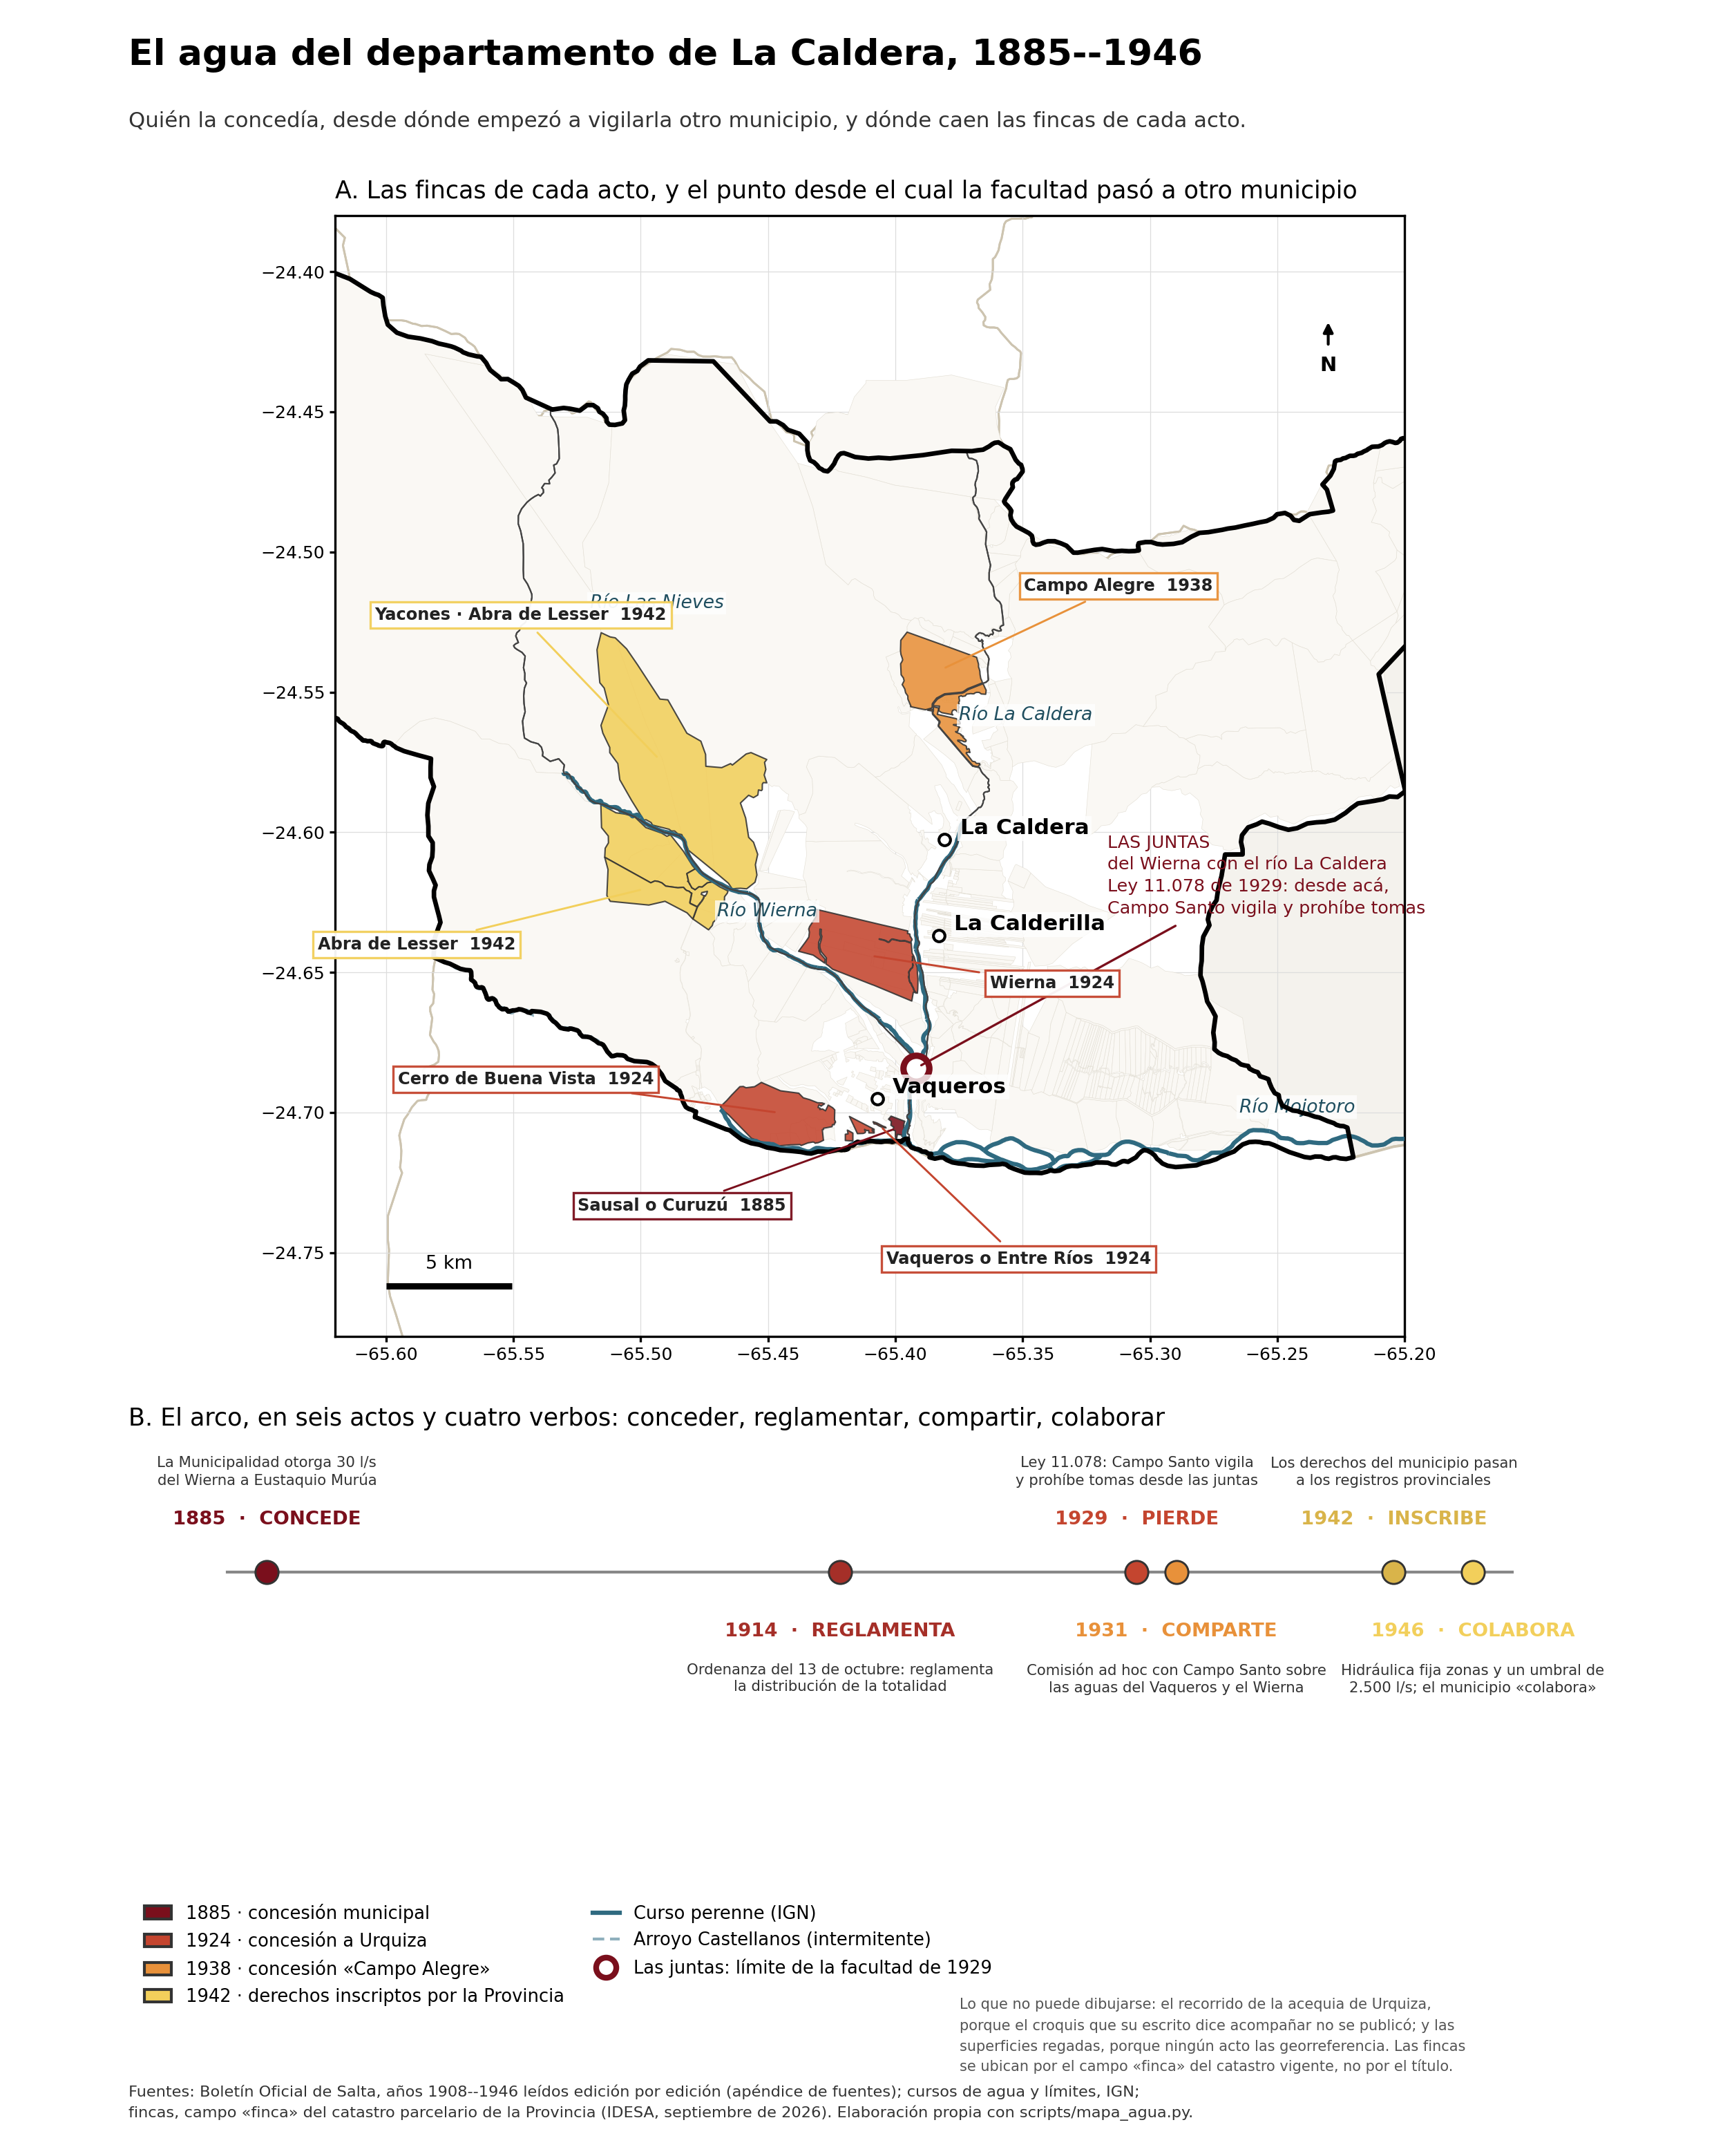
\includegraphics[width=\textwidth,height=0.88\textheight,keepaspectratio]{fig-agua-actos.png}
\caption[El agua del departamento de La Caldera, 1885--1946]{\textbf{El agua del departamento
de La Caldera, 1885--1946.} \textbf{Arriba}, las fincas que nombra cada uno de los actos de
agua que el archivo registra, coloreadas por el año del acto, sobre los cursos del IGN y el
límite departamental; el círculo marca \textbf{las juntas del Wierna con el río La Caldera},
que es el punto desde el cual la Ley 11.078 de 1929 autorizó a la Municipalidad de Campo Santo
---hoy General Güemes--- a vigilar y prohibir bocas-tomas. \textbf{Abajo}, el arco completo en
seis actos: conceder (1885), reglamentar (1914), perder (1929), compartir (1931), inscribir
(1942), colaborar (1946). \textbf{Lo que no puede dibujarse}: el recorrido de la acequia de
Urquiza, porque el croquis que su escrito dice acompañar no se publicó, y las superficies
regadas, porque ningún acto las georreferencia; las fincas se ubican por el campo «finca» del
catastro vigente y no por el título. Elaboración propia; dibujo de
\texttt{scripts/mapa\_agua.py} del repositorio \texttt{mapas\_caldera} (apéndice
\ref{cap:fuentes}).}
\label{fig:agua}
\end{figure}

\chapter{¿Es esto un dispositivo?}
\label{cap:prospectiva}

Este libro se llama \textit{El dispositivo caldereño} y nunca definió la palabra. La usó decenas de veces, la puso en la tapa y la heredó del volumen anterior, pero no la sometió a la
misma exigencia que le impuso a cada expediente.

\textbf{Este capítulo hace eso, y con el mismo criterio que el resto: el término se conserva si
lo documentado lo sostiene, y se abandona si no.} De esa respuesta depende, además, la única
pregunta que el libro no ha contestado: qué va a pasar acá.

\begin{cautela}
\textbf{Es el único capítulo del libro que proyecta, y el único que argumenta más de lo que documenta} ---el capítulo \ref{cap:infraestructura} también relee, pero para describir, y el \ref{cap:plan} propone, pero no pronostica---. Casi no agrega hechos nuevos: reordena los que los veintiséis capítulos anteriores establecieron, y la única novedad ---el lanzamiento del PDES 2050--- se consigna como tal. Quien lo lea salteado debe saber que \textbf{acá se razona, y que en
el resto se transcribe}.
\end{cautela}

\section{Qué quiere decir la palabra}

El término viene de Michel Foucault, que lo usó en 1977 para nombrar una clase de objeto que la
palabra «institución» no alcanza a describir. Un dispositivo es, en su formulación, un
\textbf{conjunto deliberadamente heterogéneo}: discursos, instituciones, disposiciones
arquitectónicas, decisiones reglamentarias, leyes, medidas administrativas, enunciados
científicos. Lo que lo constituye no es ninguno de esos elementos sino \textbf{la red que puede
establecerse entre ellos}. Y tiene una propiedad decisiva: cumple una \textbf{función
estratégica} y responde a una urgencia, \textbf{sin que haya un estratega}.

Giorgio Agamben amplió el término en 2006 hasta volverlo casi ilimitado: dispositivo es
cualquier cosa que tenga la capacidad de capturar, orientar, determinar, interceptar, modelar,
controlar o asegurar las conductas de los seres vivos.

\begin{cautela}
\textbf{La versión de Agamben no sirve para este libro, y conviene decir por qué.} Si
dispositivo es cualquier cosa que orienta conductas, entonces todo lo es ---una ruta, una tarifa,
un horario--- y el término deja de distinguir nada. \textbf{Un concepto que no excluye nada no
prueba nada.}

Este capítulo usa la versión estricta: \textbf{red heterogénea, función estratégica, ausencia de
estratega}. Es más difícil de sostener y por eso vale más.
\end{cautela}

\section{Primera condición: la heterogeneidad}

\textbf{Se cumple, y con holgura.} Lo que este libro documenta sobre un territorio de dos
municipios incluye, en la misma trama:

Un poseedor colonial del siglo XVII, partidos policiales de 1909 y sucesiones del siglo XX \textit{(cap.\ \ref{cap:fincas})}. Una ley
de 1929 que autoriza a un municipio de otro departamento a reconcentrar el agua de esta cuenca
\textit{(cap.\ \ref{cap:aguabaja})}. Una expropiación de 1972 para un embalse que abastece a la
capital \textit{(cap.\ \ref{cap:expropiacion})}. Un código de aguas de 1998, reglamentado en 2003, con un decreto
de línea de ribera de 2002 \textit{(cap.\ \ref{cap:ribera})}. Un plan de desarrollo aprobado con carácter definitorio \textit{(cap.\ \ref{cap:pdua})}. Un código de ordenamiento municipal que declara no urbanizables las márgenes del río sin decir cuántos metros \textit{(cap.\ \ref{cap:cot})}. Veinte
concesiones de áridos ante un juzgado de minas \textit{(cap.\ \ref{cap:resistencias})}. Un
ordenamiento de bosques nativos con su ley, su cartografía y su umbral de deforestación por
cuenca \textit{(cap.\ \ref{cap:opacidad})}. Un amparo colectivo \textit{(cap.\
\ref{cap:amparo})}. Una obra vial con audiencia pública \textit{(cap.\ \ref{cap:vaqueros})}.
Contratos de promoción turística con exención de tributos \textit{(cap.\ \ref{cap:poblacion})}. Y
una gacetilla vecinal de 2018 \textit{(cap.\ \ref{cap:resistencias})}.

\textbf{Nada de eso pertenece al mismo campo, ni a la misma época, ni a la misma autoridad.} Y
sin embargo recae todo sobre el mismo suelo, y este libro pudo reconstruir la red que los une
sin forzar un solo dato.

\section{Segunda condición: la función estratégica}

\textbf{También se cumple, y este libro puede enunciarla en una frase.}

\begin{ficha}{La función, dicha con los números del libro}
El departamento \textbf{produce agua} para una ciudad que no es la suya: el embalse de Campo
Alegre con su planta de cuatro mil metros cúbicos por hora, el Acueducto Norte, la ley de 1929.

\textbf{Produce material pétreo} para esa misma ciudad: veinte concesiones sobre los cauces, y
dos de las concesionarias son contratistas de obra pública de la capital \textit{(cap.\
\ref{cap:infraestructura})}.

\textbf{Produce suelo residencial} para quienes trabajan allá: crecimiento poblacional del
58,4 por ciento en doce años, la tasa de empleo más alta de la provincia, y ---en el municipio de La Caldera--- \textbf{2,23
personas por vivienda}, el tercer valor más bajo entre sesenta municipios; en el departamento, 2,45 contra 3,13 provinciales.

\textbf{Y no recibe lo equivalente}: entre el dieciocho y el cincuenta y ocho por ciento de sus
hogares sin agua de red según la zona, más del noventa y cinco por ciento sin cloaca, y una
calzada de cinco metros y medio que no puede ensancharse.
\end{ficha}

\textbf{Tres flujos en la misma dirección, sostenidos por instrumentos de tres siglos y de
cuatro jurisdicciones distintas.} Eso es una función estratégica en el sentido preciso del
término: no una intención, sino un efecto sistemático que los elementos producen por su
disposición relativa.

\section{Tercera condición: que no haya estratega}

\textbf{Esta es la que el libro tardó más en poder afirmar, y es la que decide todo.}

\begin{ficha}{Lo que se buscó y no se encontró}
\textbf{No hay un plan que lo decida.} El PDES 2030 se aprobó con carácter definitorio invocando el artículo 77 de la Constitución provincial, y «La Caldera» aparece \textbf{dos veces en ciento setenta páginas}: en la nómina de
asistentes al Diagnóstico y en un inventario hotelero. Ese mismo plan cartografía los salares de
la puna con sus empresas y sus toneladas: \textbf{sabe territorializar cuando quiere}.

\textbf{No hay una decisión de perfil vigente.} Hubo actos que intentaron asignarle una ---la Ley 1423 (orig.\ 145) de 1934 incorporó al departamento a la región económica del olivo (capítulo \ref{cap:hacienda}) y el Decreto 12 de 1980 reconoció su área tabacalera (capítulo \ref{cap:tierra})---, pero ninguno de los dos perfiles sobrevivió, y no hay acto posterior que asigne al corredor vocación turística, agropecuaria ni residencial.

\textbf{Y el Estado lo reconoce por escrito.} El propio plan declara, en 2012, que el
crecimiento del área metropolitana fluyó «\textit{espontáneamente, \textbf{sin
planificación}}», y que hay que «\textit{paliar los efectos de la falta de previsión}».
\end{ficha}

\textbf{No hay estratega.} Y no porque este libro no lo haya encontrado, sino porque el
instrumento que debería contenerlo declara que no existe.

\textbf{Y hay una prueba más, de otra clase, que los barridos de 1918 y 1919 pusieron a la vista.}
En marzo de 1918 un gobierno decidió, por un umbral de \textbf{renta}, que catorce departamentos
pasaban a ser Municipalidades electivas, y a La Caldera se lo revocó rehaciendo la cuenta. En
enero de 1919 el gobierno siguiente declaró que ese umbral no existía: que el artículo en que se
fundaba estaba derogado y que lo que la Constitución exige es un umbral de \textbf{población}
(capítulo \ref{cap:siglo}). \textbf{Doce meses, dos gobiernos, dos reglas distintas para la misma
pregunta, y ninguno de los dos citando al otro.} Un dispositivo con estratega tiene una regla; lo
que el archivo muestra en estos dos años es que \textbf{ni siquiera la regla estaba establecida},
y que el resultado ---el departamento sin gobierno propio--- salió igual por los dos caminos.

\textbf{Y el barrido de 1922 muestra hasta dónde llegó ese resultado.} El 18 de abril de ese año
un Interventor Nacional designa las Comisiones Municipales de los departamentos «\textit{que en
la actualidad carecen de ella}», y La Caldera va primera en la lista (capítulo
\ref{cap:siglo}). \textbf{No es que el departamento tuviera un gobierno débil: no tenía ninguno},
y el archivo no registra cuándo lo perdió. Cuatro años después de la discusión sobre si debía ser
Municipalidad electiva, el cuerpo que se le discutía había desaparecido sin que ningún acto
publicado lo dijera.

\textbf{Y diecisiete meses después la Provincia intervino el que acababa de crearse.} El decreto
1161 del 24 de septiembre de 1923 declara intervenida la Municipalidad del departamento y nombra
un Interventor, a pedido de presentaciones que un expediente instruye y que no se publican
(capítulo \ref{cap:siglo}). \textbf{Con eso, el ciclo se cierra y se puede contar entero}: en
1918 el Estado resolvió que el departamento no estaba en condiciones de tener municipalidad
electiva, por un umbral de renta; en 1919 declaró que el umbral era la población; entre julio de
1921 y abril de 1922 el departamento se quedó sin Comisión Municipal sin que ningún acto lo
dijera; en abril de 1922 un Interventor Nacional se la devolvió; en septiembre de 1923 el
gobierno provincial la intervino; \textbf{y en abril de 1924, aceptadas las renuncias
«indeclinables» de dos de los miembros que quedaban, el Poder Ejecutivo designó por decreto a los
cuatro que la integrarían} ---uno de ellos el mismo que había renunciado tres meses antes, y otro
el concesionario del agua--- \textbf{«vistas las comunicaciones» de un expediente que no se
publica}. \textbf{Seis actos en siete años, ninguno de los cuales cita al
anterior, y los seis resuelven quién administra este territorio. Ninguno lo decide el
territorio}, y en ninguno de los seis hay una elección.

\textbf{Y la serie no termina ahí: llega hasta 1946 y suma dos episodios más.} En septiembre de
1930 los actos del departamento pasan a firmarlos un \textbf{Interventor Nacional}; y entre 1944
y agosto de 1946 el cuerpo municipal está otra vez \textbf{intervenido}, esta vez sin que ningún
acto publicado diga cuándo se dispuso (capítulos \ref{cap:siglo} y \ref{cap:opacidad}).
\textbf{Ocho actos en veintiocho años, y de los ocho ninguno sale de una elección.} La lámina
\ref{fig:cargos} los marca con línea vertical: 1918, 1922, 1923, 1930 y 1944.

\textbf{Y hay un noveno hecho, que no es un acto sino su ausencia}: entre julio de 1921 y abril
de 1922 el departamento estuvo \textbf{sin comisión municipal}, y el archivo no registra cuándo
la perdió. \textbf{De veintiocho años, este libro puede documentar al menos nueve en que el
cuerpo municipal no era un cuerpo electo}: los de las dos designaciones por interventor nacional,
los de las dos intervenciones y el año sin comisión.

\textbf{Ésa es la forma más pura de la tercera condición}: no hay estratega
porque, en los tramos donde el archivo deja mirar, no hay siquiera un órgano local estable al que
un estratega pudiera dirigirse.

\textbf{Y el arco del agua da la prueba positiva que a esta condición le faltaba.} Entre 1885 y
1946 el municipio pasa de \textbf{conceder} treinta litros por segundo del Wierna a
\textbf{prestar «la colaboración necesaria»} a la Dirección General de Hidráulica, en seis actos
de los cuales \textbf{ninguno deroga al anterior} (lámina \ref{fig:agua} y capítulo
\ref{cap:infraestructura}). \textbf{Eso es exactamente lo que este capítulo entiende por
dispositivo y no por plan}: nadie decidió quitarle la facultad, y sin embargo al final no la
tiene. \textbf{Si hubiera habido un estratega, habría un acto que la deroga}; lo que hay es una
sucesión de actos que la rodean.

\textbf{Y hay una razón anterior, que el archivo temprano dejó ver y que vale más que la
anterior porque no depende de lo que un plan declare de sí mismo: en este departamento nunca
hizo falta un estratega, porque el conjunto de personas que podían ocupar los cargos era
demasiado chico.} En 1909, con ciento setenta y siete inscriptos en el registro cívico, el
hombre que clasificaba a los contribuyentes para el impuesto de patentes pasó a mandar la
policía del departamento; el juez de paz suplente era, al mismo tiempo, comisario suplente y
miembro de la comisión municipal; el comisario auxiliar de un partido era propietario en ese
partido; y el presidente municipal que firmaba el cuadro de rentas administraba la finca más
grande del territorio, que su propia familia tenía en condominio (capítulos \ref{cap:fincas} y
\ref{cap:siglo}). Los tres reemplazos que la comisión municipal necesitó ese año salieron del
mismo jurado de patentes del año anterior.

Eso no prueba acuerdo ni parentesco, y este libro no lo afirma. Prueba algo distinto y más
duradero: que \textbf{la coincidencia entre quien regula y quien es regulado no necesitó
producirse, porque venía dada}. Seis años más tarde vuelve a ocurrir sin que nadie lo decida: en diciembre de 1915 el juez de paz del departamento es el comisionado que clasifica sus patentes, y los dos jurados que resolverán los reclamos contra esa clasificación son dos de sus propietarios mayores, con un miembro de la comisión municipal de suplente (capítulo \ref{cap:siglo}). Un siglo después, el capítulo \ref{cap:defensas} encuentra la misma
forma con otros nombres: la sociedad que en un mismo año es concesionaria de áridos sobre tierra
fiscal, oferente admisible en la obra que protege el acueducto y contratista directa de su
reparación. \textbf{Y una tercera vez en 1918}, ya no en el pueblo chico de 1909 sino bajo una Intervención
Nacional: el presidente de la Mesa N.\ 1 del Colegio Electoral del departamento es, en el mismo
año, el juez de agua de uno de sus dos distritos, nombrado por el Interventor a propuesta del
propio municipio; su segundo suplente de mesa es el mismo Augusto Regis\index{Regis, Augusto}
que el archivo registra desde 1908, y el apellido que los deslindes de la Calderilla de 1917
registran como propietario lindero figura en la mesa de Mojotoro como autoridad electoral
(capítulo \ref{cap:siglo}). \textbf{Tres veces en nueve años, con tres juegos de nombres y bajo
tres regímenes distintos ---gobierno electo, gobierno electo otra vez, intervención federal---,
y ninguna de las tres necesitó que nadie la arreglara. \textbf{Y una cuarta en 1919}, con el
Presidente del Senado en ejercicio del Ejecutivo.} La condición se sostiene, entonces, por dos vías
independientes: el instrumento de 2012 que declara que nadie planificó, y el archivo de 1909 que
muestra por qué no hacía falta que nadie lo hiciera ---una serie, no un episodio: 1909,
1915, 1918, 1919, 1920 y 1921, con seis juegos de nombres y bajo cinco gobiernos distintos. En 1919, dos
de los cinco miembros de la Comisión Municipal son, en el mismo trimestre, comisarios de partido
bajo las órdenes del Jefe de Policía, y ese mismo cuerpo eleva las ternas de jueces de paz; y el
veedor del Código Rural de Chalcanio de 1909 es, diez años después, el comisario auxiliar de ese
mismo paraje (capítulo \ref{cap:siglo}). \textbf{Y en 1920 la superposición cambia de especie},
que es lo que la vuelve interesante: ya no es un cargo que coincide con otro cargo, sino que
\textbf{uno de los tres candidatos a diputado por el departamento es quien dos años antes había
pedido las dos únicas concesiones mineras que el Boletín registra sobre este suelo}. Coincidencia
de nombre y no identificación registral, y aun así es el primer caso de la serie en que quien
pide una concesión sobre el departamento se presenta a representarlo. \textbf{Y en 1921 vuelve a
cambiar de especie}: \textbf{Daniel Linares}\index{Linares, Daniel} es, el mismo año, primer
suplente de la mesa 1 del departamento y el propietario que dos de los cuatro rumbos del deslinde
de la finca El Angosto declaran como lindero (capítulo \ref{cap:siglo}). \textbf{Y en 1922 una séptima, bajo otra Intervención Nacional y con la forma más neta de
todas}: \textbf{Jorge Rauch} es comisario de policía del departamento desde marzo y miembro de su
Comisión Municipal desde abril; \textbf{Carlos F.\ Matienzo}\index{Matienzo, Carlos} acumula, con quince días de
diferencia, el juzgado de paz propietario y el Registro Civil del mismo departamento; y
\textbf{Daniel Linares}\index{Linares, Daniel}, que en enero recibe la correspondencia electoral del departamento, en
abril integra el cuerpo que lo gobierna (capítulo \ref{cap:siglo}). \textbf{Y en 1923 una octava, que cambia de escala}: el escrito con que
Francisco S.\ Urquiza\index{Urquiza, Francisco S.} pide la primera concesión de agua del
departamento declara que su acequia atraviesa la finca Vaqueros, «\textit{de propiedad de los
herederos Toranzos y doctor \textbf{Carlos Serrey}}»\index{Serrey, Carlos}, y cinco meses después
ese mismo Carlos Serrey se incorpora al Senado provincial por Cerrillos, en la misma nómina que
trae al senador por Caldera (capítulo \ref{cap:siglo}). \textbf{Ya no es un cargo que coincide con
otro cargo dentro del departamento: es el propietario del suelo que la obra debe atravesar
sentado en la legislatura de la provincia que concede el agua.} Coincidencia de nombre y no
identificación registral. \textbf{Y en 1924 una novena, que es la más completa de todas.} El mismo Urquiza\index{Urquiza, Francisco S.}
aparece cuatro veces en un año y en cuatro calidades: \textbf{en enero} recibe la concesión de
agua, fundada en el informe de la Comisión Municipal del departamento; \textbf{en marzo} figura
como propietario lindero en el deslinde de la finca vecina; \textbf{en abril} el decreto 1576 lo
designa \textbf{miembro de esa misma Comisión Municipal}; y \textbf{en octubre} preside la mesa de
Vaqueros (capítulo \ref{cap:siglo}). \textbf{Tres meses separan al beneficiario de la primera
concesión de agua del departamento del cuerpo cuyo informe la fundó}, y veinte años después el
mismo hombre es el mayor de los cuarenta y siete titulares que publica el revalúo de 1944.
\textbf{Y el barrido de 1925 agrega una quinta calidad}: el decreto 2674 del 25 de junio de ese
año nombra subcomisario \textit{ad honorem} de Vaqueros a Antonio Agüero «\textit{en reemplazo de
D.\ Francisco S.\ Urquiza}», de modo que el mismo hombre era también \textbf{la autoridad policial
del paraje}, sin sueldo y sin que su nombramiento aparezca en ningún tramo leído.
\textbf{Y en 1940 una décima, que es la más directa de todas}: el Boletín
identifica al solicitante de una ayuda para las fiestas patronales del pueblo
como «\textit{el señor presidente de la comisión municipal del distrito de la
Caldera, \textbf{diputado provincial don Augusto Regis}}»\index{Regis, Augusto}
(capítulo \ref{cap:siglo}). \textbf{No es un cargo que coincide con otro dentro
del departamento: es la misma persona presidiendo el municipio y sentada en la
Legislatura que lo regula}, y lleva para entonces cuatro reelecciones seguidas
por decreto y dieciocho años entrando y saliendo de ese cuerpo. \textbf{Y en 1942 una undécima, que completa el cuadro}: el mismo Augusto
Regis\index{Regis, Augusto} es nombrado \textbf{comisario de policía de La
Caldera} mientras preside la Comisión Municipal del distrito ---reelecto por
decreto ese año y el siguiente--- y ocupa una banca de diputado provincial
(capítulo \ref{cap:siglo}). \textbf{Presidente del cuerpo que gobierna el
departamento, comisario de su policía y legislador de la provincia que lo
regula, a la vez y en actos publicados.} \textbf{Y la relectura de 1911 y 1912 agrega una que es
anterior a todas menos la primera, y de otra especie}: en octubre de 1911 la Provincia crea, \textit{ad
honorem}, una oficina del Registro Civil en la estación Mojotoro y la pone a cargo de Benjamín
López\index{López, Benjamín}, subcomisario del partido de la estación; en diciembre de 1912 el
mismo López pasa a comisario del partido, y en el juicio de ese año declara como jefe de la
estación del ferrocarril (capítulo \ref{cap:presencia}). \textbf{El registro de las personas, la
policía y el ferrocarril, en un solo hombre, en el mismo paraje y sin sueldo por el primero.}
\textbf{Doce ocurrencias en treinta y tres años, y ya no todas del mismo tipo}: cargo con cargo, concesionario con
candidato, autoridad electoral con propietario del suelo que se deslinda, dos ramas del
Estado local ---la justicia de paz y el registro de las personas--- en la misma persona y en la
misma quincena, propietario afectado con legislador provincial, concesionario de agua
con miembro del cuerpo que informó su concesión, y tres funciones del Estado en un solo hombre
allí donde llegaba el tren.

\begin{cautela}
\textbf{Conviene distinguir esto de dos cosas que no son.}

\textbf{No es una conspiración.} Nadie se reunió a decidir que La Caldera proveyera agua, piedra
y dormitorios. Los actos que producen ese resultado tienen cada uno su fundamento propio y su
autoridad competente, y este libro no encontró uno solo que sea ilegal.

\textbf{Y no es un accidente.} Un accidente no se repite durante tres siglos en la misma
dirección. Lo que hace que los tres flujos vayan siempre hacia el mismo lado no es el azar: es
que \textbf{los instrumentos están dispuestos de manera tal que ése es el resultado que
producen}, y nadie tiene a su cargo mirar el conjunto.
\end{cautela}

\section{Entonces sí, y el término dice algo}

Las tres condiciones se cumplen. \textbf{La Caldera es un dispositivo en el sentido estricto: una
red heterogénea de instrumentos que cumple una función estratégica sin que nadie la haya
diseñado.}

\textbf{Y decirlo así no es una figura literaria: tiene consecuencias prácticas.}

Si hubiera un diseño, la corrección sería política: cambiar la decisión. \textbf{Como no lo hay,
la corrección es institucional}: producir el órgano, el registro o el criterio que hoy no
existen. Por eso el apéndice \ref{cap:propuestas} contiene veintiséis propuestas normativas y
ninguna denuncia.

Si hubiera un culpable, el libro sería una acusación. \textbf{Como no lo hay, es un inventario}:
doscientos setenta y ocho pedidos, ordenados en doce secciones ---once por destinatario y una sobre la vida cotidiana---, y la mayoría pide lo que la propia norma
manda producir.

\section{Qué viene, entonces}

\begin{cautela}
\textbf{Todo lo que sigue es prospectivo.} No documenta: proyecta sobre lo documentado.
Cualquiera de estas líneas puede no ocurrir, y ninguna debe citarse como hallazgo de este libro.
\end{cautela}

\subsection*{Lo que la dinámica indica}

Si no hay diseño, lo que viene no lo decide nadie: lo produce la disposición de los elementos.
Y esa disposición apunta en una dirección \textbf{que no es la que el propio departamento se
atribuye}.

\textbf{No es turismo.} Hoteles y restaurantes ocupan a doscientas dieciocho personas, el 3,49
por ciento: por debajo del promedio provincial y por debajo de la capital. El servicio doméstico
emplea al doble. Las veinte canteras, a cincuenta y una personas.

\textbf{No es agricultura.} Ciento noventa y tres personas, sobre una superficie declarada que
cayó un ochenta y ocho por ciento ---aunque el capítulo \ref{cap:tierra} muestra que lo que cayó
fue sobre todo declaración de monte, no de cultivo---.

\textbf{Es residencia.} Población en alza sostenida, empleo alto, viviendas semivacías, el Estado como principal empleador y una parte del trabajo, presumiblemente, en la capital. \textbf{Lo que los números describen es un suburbio residencial y de fin de semana de una
capital de medio millón de habitantes.}

\subsection*{Lo que lo acelera}

\textbf{La ruta.} La pavimentación del tramo entre la rotonda de avenida Bolivia y el puente del
río La Caldera, expediente 0110033-243466/2021-181, con estudio de impacto y audiencia convocada para noviembre de 2023. El capítulo \ref{cap:vaqueros} establece el mecanismo: la infraestructura que reduce
la fricción con la capital valoriza el suelo.

\textbf{Y no es nuevo.} Entre 1923 y 1945 lo que el Estado construyó en el departamento fueron
caminos, y los caminos seguían de largo, hacia Campo Santo, Güemes, Jujuy y la capital (capítulo
\ref{cap:presencia}). La ruta que hoy acelera la valorización es la capa más reciente de la
inversión que el Estado sostuvo sin pausa en ese tramo del archivo.

\textbf{El agua.} La red se está extendiendo ---barrio Santiago Apóstol, septiembre de 2026--- y
el capítulo \ref{cap:redes} muestra que la factibilidad hídrica es la condición práctica del
fraccionamiento.

\subsection*{Lo que lo limita, y es lo que este libro no esperaba}

\textbf{La ladera está ocupada.} El titular provincial de Vialidad Nacional declara en agosto de
2026 que la calzada tiene cinco metros y medio, y la nota de prensa que recoge esa declaración
agrega, sin atribuírselo entre comillas, que \textbf{los emprendimientos privados sobre
las laderas, muchos sin autorización, complican cualquier ampliación futura del corredor}
(capítulo \ref{cap:vaqueros}).

\textbf{La pendiente está protegida.} El nuevo artículo 14 de la Ley 7543 pone en Categoría II
todo lo que tiene \textbf{pendiente superior al quince por ciento}, que es exactamente esa
ladera.

\textbf{Y desde diciembre de 2024 hay un permiso más.} El artículo 20 reformado exige que toda
urbanización con cambio de uso de suelo en zona categorizada cuente con \textbf{la no objeción
de la autoridad forestal}.

\textbf{Y el bosque de esta cuenca no es categorizable.} Es el límite más duro de los cuatro y
el que este capítulo no había puesto en esta lista, aunque el libro lo documenta: el capítulo
\ref{cap:opacidad} establece, con las capas del propio informe técnico de la Ley 8483, que la
cuenca Mojotoro--Lavayén ---que ocupa el setenta y nueve por ciento del departamento--- figura
excedida en su umbral máximo de deforestación y tiene \textbf{cero hectáreas categorizables a
verde}. Según el criterio que el mismo informe enuncia, en una cuenca excedida no se autorizan
proyectos de cambio de uso de suelo. \textbf{Desde enero de 2025, entonces, el desmonte de bosque
nativo está vedado en casi todo el departamento}, y a diferencia de los otros tres límites éste
no depende de una pendiente, de un ancho de calzada ni de una decisión futura: sale de una
cuenta hecha sobre la historia productiva de la cuenca.

\textbf{Puesto junto, eso describe un techo.} El valle está fraccionado, la ladera está ocupada
y además protegida, el bosque de la cuenca no es categorizable, y la ruta no puede crecer. \textbf{El dispositivo que produjo este
territorio está llegando al límite de lo que puede producir sin decisión.}

\subsection*{Y una ventana que está abierta ahora}

\begin{ficha}{Plan de Desarrollo Estratégico Salta 2050}
El \textbf{18 de mayo de 2026} se lanzó en el Centro de Convenciones de Salta el proceso
participativo de elaboración del \textbf{PDES 2050}, bajo el nombre «Salta 2050: Diálogos para
construir el futuro».

Financiamiento del \textbf{Consejo Federal de Inversiones}. Apertura a cargo del presidente del
Consejo Económico Social. Articulación a través de la Coordinación de Relaciones Políticas y
Planificación Estratégica. Jornada abierta al público \textbf{con cupo limitado} e inscripción
previa.

Se presenta como \textbf{actualización del PDES 2030}, creado en 2009 y actualizado en 2018.
\end{ficha}

\textbf{El plan que fijará el horizonte 2050 no existe todavía: se está escribiendo.}

En 2011 la Intendencia de La Caldera participó del Diagnóstico y el departamento apareció dos
veces en el documento final. \textbf{En 2026 el proceso empezó de nuevo, y todavía no está
decidido si esta vez aparece.}

\textbf{Y del lanzamiento se sabe algo más, que conviene poner al lado.} En un plenario de la
Cámara de Senadores provincial, representantes del Consejo Económico y Social expusieron la
puesta en marcha del plan y dejaron tres definiciones. La primera: que el plan busca adaptar las
metas a una provincia que ---según esa exposición--- transformó su matriz económica hacia
\textbf{la minería, la agroindustria y el turismo}. La segunda: que incorporará prospectiva por
escenarios y una \textbf{visión regionalizada}. Y la tercera: que el Consejo define metas,
mientras que el «cómo hacerlo» sigue siendo facultad exclusiva de los poderes públicos, y que
sus dictámenes técnicos son \textbf{no vinculantes}.

\begin{cautela}
Las tres definiciones alcanzan a este departamento, y en direcciones distintas.

\textbf{Las tres matrices que el plan declara son, justamente, las tres que este capítulo acaba
de descartar para el corredor.} La minería de La Caldera son veinte concesiones de áridos que
ocupan a cincuenta y una personas; el turismo, doscientas dieciocho; la agroindustria, ciento
noventa y tres sobre una superficie declarada que cayó. Si el plan 2050 se organiza sobre esas
tres matrices, el corredor vuelve a quedar sin casillero por la misma razón por la que no lo
tuvo en 2030, y no es exclusión: \textbf{lo que este departamento produce ---agua, piedra y
dormitorios--- no es una matriz productiva en el sentido en que esos planes usan la palabra.}

\textbf{La visión regionalizada es la única puerta.} Es el primer compromiso metodológico, en
los diecisiete años de planificación estratégica provincial que este libro repasa, que obliga a
bajar del agregado provincial al territorio. El reproche de este libro al PDES 2030 fue
exactamente ése: que sabe territorializar cuando quiere y que sobre este corredor no lo hizo.

\textbf{Y el carácter no vinculante marca la distancia con 2030.} Aquel plan se aprobó por
decreto invocando el artículo 77 de la Constitución provincial, que le daba «carácter
definitorio», y aun así este libro no encontró un solo acto del corredor que lo invoque
(capítulo \ref{cap:pdua}). Si lo que viene son dictámenes no vinculantes, la distancia entre el
plan y el expediente no se acorta: queda declarada de entrada.
\end{cautela}

\textbf{Y hay una continuidad que corresponde registrar, sin imputarle nada.} El PDES 2030 nació
en 2009 como iniciativa de la \textbf{Fundación Salta} (capítulo \ref{cap:pdua}). Diecisiete años
después, esa misma fundación integra el Consejo Económico y Social que impulsa la actualización,
y quien preside el Consejo es su vicepresidente. \textbf{No se sigue de eso ninguna imputación}:
se sigue que el órgano que fija el horizonte de largo plazo de la provincia tiene la misma
continuidad de personas e instituciones que este libro documenta en escalas mucho más chicas, y
que esa continuidad es, ella misma, un rasgo del objeto.

\begin{cautela}
\textbf{Toda esta subsección se apoya en partes de prensa y no en instrumentos.} Los partes del
Gobierno de la provincia del 12 y del 18 de mayo de 2026, el parte de la Cámara de Senadores
sobre el plenario ---que no consigna su fecha---, y las crónicas de los participantes
institucionales, consultados el 21 de septiembre de 2026. \textbf{No hay todavía acto
administrativo que cree el proceso}, ni términos de referencia publicados, ni cronograma. Lo que
se afirma aquí es que esas declaraciones se hicieron, no que el plan vaya a decir eso.
\end{cautela}

\begin{cautela}
\textbf{Ésa es la única afirmación de este capítulo que no es una proyección sino una
constatación:} hay un proceso de planificación abierto, con inscripción pública, y el
departamento tiene los materiales para presentarse a él. Este libro es uno de ellos; el apéndice
\ref{cap:propuestas}, otro.

\textbf{Lo que este libro no puede decir es si servirá de algo.} Un proceso participativo con
cupo limitado, en la capital, en día hábil, tiene las mismas barreras de acceso que la audiencia
pública del capítulo \ref{cap:vaqueros} y que el expediente en horario de oficina del capítulo
\ref{cap:ribera}. \textbf{El dispositivo también regula quién puede participar en las decisiones
que lo modificarían}, y eso es, exactamente, lo que la palabra nombra.
\end{cautela}

\section{Lo que refutaría todo este capítulo}

\textbf{Tres hallazgos lo desarmarían, y los tres son posibles.}

\textbf{Uno.} Que aparezca un acto de gobierno ---un decreto, un convenio, un acta--- que asigne al corredor, en el período en que se formó como periferia metropolitana, un perfil productivo que se haya sostenido. Si existe, hay estratega y el término no corresponde. \textbf{Y hay un tercer acto, incorporado al cierre, que conviene poner a prueba acá porque es el
que más se acerca}: el decreto 1.660 del 24 de abril de 1918, que resuelve que La Caldera
«\textit{no está en condiciones de ser administrado por una Municipalidad electiva}» y la
devuelve a Comisión Municipal (capítulo \ref{cap:siglo}). Es un acto de gobierno, fechado,
firmado y fundado, que decide sobre la condición institucional del departamento, y es la pieza
más parecida a un estratega que este relevamiento encontró. \textbf{No cumple la condición, y
conviene decir por qué}: no le asigna al corredor ningún perfil ni ningún destino ---se limita a
aplicar un umbral de renta a una planilla contable---, y cuatro semanas después el decreto 50 lo
extendió a los catorce departamentos por igual. Un criterio general aplicado con una cuenta no es
una decisión sobre este territorio. \textbf{Pero es el candidato más serio que el libro tiene, y
se deja consignado como tal para que se lo pueda discutir.} \textbf{El decreto 510 del 18 de abril
de 1922, que le devuelve al departamento su Comisión Municipal, es el candidato simétrico y
tampoco cumple}: decide sobre la existencia misma del órgano local ---que es más que decidir su
categoría---, pero lo hace en un acto general que alcanza a todos los departamentos «que en la
actualidad carecen de ella» y no le asigna al corredor ningún perfil. \textbf{Los dos actos
deciden qué gobierno tiene este territorio y ninguno de los dos dice para qué sirve}, que es
exactamente la diferencia entre un umbral y una estrategia. Los dos que este libro encontró ---el olivo en 1934 y el tabaco reconocido en 1980--- no cumplen esa condición: ninguno de esos perfiles se sostuvo, lo que es compatible con la ausencia de estratega. \textbf{Hay un tercer candidato, y es el que más cerca está de refutar este capítulo}: que el departamento haya sido pensado, y no sólo usado, como lugar de veraneo de la clase alta de la capital. El capítulo \ref{cap:poblacion} reúne lo que el archivo da a favor ---las casas quinta de 1927 y 1929, las truchas sembradas en 1940 y 1942, la iglesia ampliada en 1935, los apellidos de gobierno en el revalúo de 1944--- y lo que da en contra ---el olivo, el tabaco, el camino eliminado del plan en 1944, el puente postergado en 1935---, y concluye que el uso fue el más antiguo pero no fue asignado. \textbf{Si el padrón catastral de 1944 mostrara que sus titulares domiciliaban mayoritariamente en la capital, esa conclusión habría que revisarla, y con ella esta condición.}

\textbf{Dos.} Que el procesamiento censal de lugar de trabajo muestre que la mayoría de los
ocupados del departamento trabaja \textbf{dentro} de él. Si así fuera, la lectura residencial se
cae y con ella toda la sección prospectiva.

\textbf{Tres.} Que los organismos, requeridos, produzcan los documentos que este libro no
encontró: el aforo, el balance hídrico, el padrón de concesiones, el atlas del Código. Si todo
eso existe y simplemente no se publicó, \textbf{el problema es de publicidad y no de diseño
institucional}, y buena parte del apéndice \ref{cap:propuestas} sobra.

\textbf{Los tres se resuelven con los pedidos del apéndice \ref{cap:pedidos}}, ninguno de los
cuales había sido presentado al cerrarse este manuscrito.

\chapter{Qué habría que hacer}

\label{cap:plan}
\begin{cautela}
Este capítulo es, junto con el apéndice \ref{cap:propuestas}, el único lugar del libro donde se propone algo, y conviene decir con
precisión qué es y qué no es.

Va como capítulo y no como apéndice porque es prosa y no aparato, y porque sigue
directamente al anterior: aquel describe qué es este territorio; éste, qué podría hacerse.
Pero conviene que el lector lo separe con nitidez de los veintisiete capítulos que lo preceden.

\textbf{No es un plan técnico.} Este trabajo sostiene, capítulo tras capítulo, que faltan los
datos con los que se planifica: no se afora el río desde 1986 --- las cinco estaciones de la cuenca están cerradas y sus series no alcanzan el mínimo que la propia norma exige ---, no se conoce el antecedente dominial de las matrículas centrales, no se publicaron las cotas de inundación ni el padrón de servicios, y el ancho de la franja no urbanizable del río no está expresado en metros en ninguna parte del Código que la establece. Proponer obras concretas sobre esa base sería incurrir en lo mismo que el libro
señala.

\textbf{Es un plan institucional.} Enumera qué hay que medir antes de decidir, qué hay que
decidir, quién tiene competencia para hacerlo y en qué orden. Nada de lo que sigue requiere
información que este libro no tenga: requiere decisiones.

Y tiene un fundamento que conviene enunciar de entrada, porque es lo que lo separa de una
lista de deseos. \textbf{Casi todo lo que se propone aquí ya se hizo alguna vez en este mismo
departamento}, y el cuerpo del libro lo documenta. No hay que inventar instrumentos: hay que
volver a usar los que existen.
\end{cautela}

\section{Primero: lo que no se puede planificar sin medir}

Cuatro mediciones faltan, y sin ellas cualquier plan es una apuesta. Las cuatro son
producibles en meses, no en años, y ninguna requiere legislación nueva.

\textbf{Aforar los ríos.} En 1924 el Departamento de Obras Públicas dejó constancia escrita
de que no podía informar sobre el caudal del río Wierna «en razón de no haberse efectuado
aforos de los ríos de la Provincia». En 2015, el procedimiento de línea de ribera seguía
poniendo los aforos en primer lugar de prelación --- con series de cincuenta años --- y
resolviéndose en la práctica por método geológico-geomorfológico. \textbf{Cien años después, la cuenca no tiene una sola estación de aforo en funcionamiento: la última cerró en 1986.}

Sin aforos no se sabe cuánta agua hay, cuánta se está concediendo ni cuánta queda. El
capítulo \ref{cap:loteo} documenta tres gestiones de abastecimiento poblacional con tratamientos distintos
y sin fundamento explícito; el capítulo \ref{cap:politica} documenta que el mismo desconocimiento sirvió, en
1936, para negarle una indemnización a quien había ganado su juicio. \textbf{La ausencia de
aforos no es neutral: favorece a quien decide, porque vuelve indiscutible cualquier decisión.}

\textbf{Publicar las cotas y las líneas de ribera con sus coordenadas.} Doce de quince determinaciones del período relevado publicaron sus coordenadas; de las tres que no lo hicieron, las dos referidas a un inmueble recaen sobre suelo en proceso de loteo, condición que comparten otras dos que sí las publicaron. Publicarlas todas es un acto administrativo de una página, y hacerlas legibles ---las del pueblo están sólo en una imagen escaneada--- es otro.

\textbf{Levantar el estado dominial de las fincas del corredor.} El departamento está
catastrado desde 1929. El registro existe, funciona y no es consultable sin arancel ni
presencia física. Un informe de dominio de las matrículas 4.366 y 6.558 --- las dos que
atraviesan este libro --- cuesta lo que cuesta un trámite y contestaría la pregunta central
del capítulo \ref{cap:loteo}.

\textbf{Publicar el padrón de servicios.} Qué manzanas tienen red de agua, cuáles cloaca,
cuáles gas, y cuáles no. Sin ese mapa no se puede saber si un loteo nuevo está donde hay
infraestructura o donde no la hay, que es exactamente lo que la Ordenanza 437 de Vaqueros se
propuso evitar en 2015.

\section{El río}

\subsection*{Lo que el propio Estado ya diagnosticó}

En diciembre de 1935, la Dirección General de Obras Públicas elevó un informe que sigue
siendo la mejor descripción disponible del problema. Identificó que el río se bifurca en tres
brazos cuatro kilómetros aguas arriba del pueblo, que el de la margen derecha se lleva la
mayor parte del caudal y que toma una curva brusca al pasar junto a las casas. Y propuso
intervenir \textbf{en la bifurcación} y no junto a las viviendas.

Ese informe agregó algo más: dijo que las obras que autorizaba eran provisorias y servirían
para «adquirir experiencia sobre el comportamiento del Río», de modo que después «se puedan
proyectar obras más duraderas».

\textbf{Ese estudio nunca se hizo.} Noventa y un años después, lo que se sigue construyendo
son espigones de emergencia, bateas y muros de contención.

\subsection*{Qué habría que hacer}

\textbf{Encargar el estudio que falta desde 1935.} Un estudio hidrológico e hidráulico de la
cuenca completa, con una serie de aforos que hoy no se produce y modelización de crecidas. Es la
condición de todo lo demás, y es lo que la sentencia de 2021 ordena cuando manda privilegiar
infraestructura verde por sobre la gris: no se puede decidir qué obra corresponde sin saber
cómo se comporta el río.

\textbf{Crear una autoridad de cuenca.} El río La Caldera nace en un municipio, atraviesa
otro, cambia de nombre y desemboca en un tercer departamento. El capítulo \ref{cap:redes} documenta que en
1929 la Provincia resolvió ese problema \textbf{repartiendo el río}: le dio a la
Municipalidad de Campo Santo potestades sobre el tramo que le importaba, incluida la de
prohibir nuevas tomas. Noventa y siete años después, ninguna jurisdicción administra el
conjunto del cauce, la extracción de áridos se concesiona en ambas márgenes sin autoridad
común, y la única figura metropolitana que la provincia construyó para el corredor es la del
transporte de pasajeros.

La Ley 7322 demuestra que la Provincia sabe crear autoridades metropolitanas cuando decide
hacerlo. Que exista una para los colectivos y ninguna para la cuenca no es un problema
constitucional: es una decisión sobre qué se administra en escala metropolitana y qué no.

\textbf{Y evaluar el efecto acumulado de un siglo de intervenciones.} Este libro documenta
obras sobre el mismo cauce en 1910, 1911, 1935, 1936, 1938, 1940, 1945, 1951, 1980, 2001, 2010, 2014, 2015, 2016--2017, 2023 y 2026, por
distintos organismos, sin que ningún acto evalúe el conjunto. En 1940 el propio Estado
consignó que una obra proyectada hubo de suspenderse \textbf{porque el río desvió su curso}.
El artículo 171 del Código de Aguas exige evaluación previa para los permisos de extracción
de áridos; para las obras del propio Estado sobre el cauce no se encontró norma equivalente.
Establecerla es una decisión de la autoridad de aplicación.

\section{El suelo}

\subsection*{Los loteos que ya existen}

Nada de lo que sigue propone desconocer derechos adquiridos, y conviene decirlo: quien compró
un lote de buena fe no es responsable de las omisiones del procedimiento que lo aprobó.

\textbf{Determinar qué está dentro de la línea de ribera y qué no.} Es información que en
buena parte ya existe: veinticinco actos entre 2013 y 2015 sobre más de veinticinco inmuebles.
Publicarla en un plano único y accesible convierte veinticinco actos dispersos en un
instrumento de gestión.

\textbf{Completar los expedientes incompletos.} El plano de El Durazno se aprobó sólo por las
etapas 1, 2 y 4; las etapas 3 y 5 no constan. Ese vacío no protege a nadie: no protege al
municipio, que no sabe qué habilitó, ni al comprador, que no sabe si su lote está aprobado.
El vecino de La Calderilla que en enero de 2026 preguntó al municipio si los loteos estaban
aprobados y no recibió respuesta está describiendo un problema con solución administrativa
simple.

\textbf{Exigir el cumplimiento de las obras comprometidas.} El Código de Ordenamiento
Territorial prevé Garantía de Ejecución de Obras y actas de Control de Avance. Aplicarlos no
requiere norma nueva. El anexo del Decreto 1682/19 prevé, además, caución por el monto de las obras y su ejecución si el desarrollador no las termina.

\subsection*{Los loteos futuros}

\textbf{Aplicar las condiciones que el propio Estado ya supo exigir.} El capítulo \ref{cap:loteo} documenta
que a Las Vertientes se le exigió resolución de línea de ribera, y que la línea se determinó
en sesenta y siete días; que el plano del Barrio La Misión descuenta la superficie del retiro
de ribera y declara reserva no urbanizable; y que a Chacras del Gallinato se le exigieron seis
condiciones, incluido un decreto del gobernador otorgando la concesión de agua.

Ninguna de esas exigencias es una invención: las tres son actos de la cartera provincial que
aprueba los loteos ---entonces, la de Economía---, sobre este mismo departamento, entre 2014 y 2015. \textbf{Que El Durazno recibiera dos
condiciones en 2021 no se explica por imposibilidad técnica.}

\textbf{Aplicar el artículo 172 del Código de Aguas.} Prohíbe instalar asentamientos poblacionales en los sectores que la Autoridad determine como inundables, y exige autorización previa ---con obras de prevención--- para toda construcción en zona ribereña. Está vigente y es de aplicación
obligatoria.

\textbf{Y usar la audiencia pública ambiental.} El artículo 49 de la Ley 7070 se aplicó en
2014 a una urbanización del departamento: la audiencia se celebró en el Centro Deportivo
Municipal de Vaqueros y el expediente completo quedó disponible en el propio municipio. El
Estado sabe acercar los expedientes cuando decide hacerlo.

\section{Agua, cloaca y gas}

\subsection*{La secuencia está invertida}

El problema de fondo no es la falta de proyectos. Este libro documenta que en 2014 la
Provincia aprobó el proyecto ejecutivo del acueducto de Vaqueros ---confeccionado por la prestadora--- y autorizó el concurso de la obra, y que en 2015 licitó redes
colectoras, colectora máxima y planta depuradora cloacal para esa localidad. Los proyectos
existieron.

Lo que documenta también es que \textbf{en los mismos años el Estado homologaba
abastecimientos privados}: a un club de campo se le exigió prever el servicio de agua «en
forma privada»; otro gestionó ciento quince metros cúbicos diarios de un río con
carácter permanente; y para cuatrocientos lotes de un tercero se tramitó un dren horizontal.

\textbf{La secuencia correcta es la que la propia Ordenanza 437 de Vaqueros enunció en
enero de 2015}: «lograr el máximo aprovechamiento de la infraestructura existente,
evitando la habilitación de nuevas áreas sin disponibilidades de extensión de las mismas». No
habilitar suelo donde no se pueda llevar servicios. El reglamento que fija cómo se aplica ese
criterio es el anexo que el Boletín nunca publicó y que el municipio terminó ofreciendo en su digesto en línea: exige agua corriente, línea de ribera, cesiones y garantía antes de vender (capítulo \ref{cap:vaqueros}).

\subsection*{Qué habría que hacer}

\textbf{Publicar el estado de ejecución de lo ya licitado.} El expediente 7807/15 de la obra
cloacal de Vaqueros: si se adjudicó, si se ejecutó, qué trazado tuvo y qué proporción del
ejido quedó servida. Es una consulta, no una obra.

\textbf{Resolver el problema de las servidumbres, que es el nudo real.} La circular
aclaratoria de esa licitación revela que la red debía atravesar propiedad privada en todos los
tramos proyectados sobre terrenos privados, y que el estudio de títulos y los planos de
servidumbre quedaban a cargo del contratista. \textbf{Cuando la infraestructura pública
depende de negociar paso por fincas privadas, el trazado sigue el mapa de la propiedad y no
el de la población.} Constituir esas servidumbres por vía administrativa, con la Dirección
General de Inmuebles interviniendo de oficio, es una decisión que cambia el problema de
naturaleza.

\textbf{Condicionar la aprobación de nuevo suelo a la factibilidad de servicios.} No es una
propuesta original: es lo que dice el considerando de una ordenanza vigente desde 2015.

\textbf{Pedir el cálculo que nadie pidió para el gas.} La red llega a Vaqueros y se detiene allí (capítulo \ref{cap:redes}). El régimen de expansión de ENARGAS permite que terceros interesados ---el municipio, un grupo de vecinos--- soliciten a la distribuidora el cálculo del Valor de Negocio de una extensión hacia La Caldera. Ese cálculo dice si la obra le corresponde a la distribuidora o cuánto deben aportar los usuarios. Pedirlo no cuesta nada y convierte una carencia en un número.

\textbf{Y decidir, explícitamente, si el abastecimiento privado es una solución transitoria o un régimen.} Hoy conviven las dos cosas sin que ningún acto las distinga. Un club de campo con
concesión permanente sobre un río y un vecino de la zona alta con camión cisterna no son dos
etapas de un mismo proceso: son dos regímenes distintos aplicados al mismo territorio.

\section{La capacidad institucional}

Nada de lo anterior se sostiene sin esto, y es lo más difícil.

Este libro documenta que el municipio de La Caldera fue clasificado en tercera categoría
el 9 de diciembre de 1931 y que la estadística provincial de 2022 lo sigue clasificando así, como a Vaqueros, aunque la ley que definía las categorías se derogó en 2018; que en 1908 vendía en licitación el derecho a cobrar sus
impuestos; que en 1922 el Interventor Nacional designaba a los cinco miembros de su comisión y le
aprobaba el presupuesto; que en 1933 gastaba en sueldos administrativos más de lo que la ley
permitía; que en 1940 debía a Sanidad cerca de un tercio de su renta anual; y que en julio de
2020 declaró por escrito no poder pagar los sueldos de su personal.

\textbf{Dejar de describir a los municipios con una categoría que ya no existe} y medirlos por lo que la Ley 8126 les exige a todos por igual ---Concejo, intendente, plan de obras, presupuesto con límite de gasto en personal, cuenta general ante la Auditoría, publicación de sus normas--- es el primer paso para dimensionar lo que les falta. La clasificación de 1931 era
correcta cuando se hizo; lo que nunca ocurrió es que volviera a hacerse, y la ley que obligaba a rehacerla ya no rige.

\textbf{Revisar la base imponible.} El capítulo \ref{cap:hacienda} documenta lotes urbanos con valuación
fiscal de tres cifras: un municipio cuya superficie urbana se multiplica sobre esas
valuaciones aumenta su obligación de servicio sin aumentar su recaudación. Un revalúo no es
un aumento de impuestos: es la condición para que la superficie loteada financie los
servicios que exige.

\textbf{Y devolverle voz sobre sus recursos.} En 1914 el municipio de La Caldera dictó una
ordenanza que reglamentaba la distribución de la totalidad del caudal de uno de sus ríos,
reconociendo los usos consuetudinarios existentes. En 1939 esa ordenanza prevaleció sobre una
solicitud de concesión provincial, y al año siguiente el Poder Ejecutivo ratificó que no
podía conceder agua de ese río. En 1924, 1938 y 1939 el dictamen o el certificado del
municipio integraron expedientes de agua y quedaron publicados.

Entre 2013 y 2015, en cambio, la Provincia dictó veinticinco actos de línea de ribera sobre la
cuenca de este departamento y en ninguno consta intervención municipal. La excepción, que la serie cuenta aparte, prueba que la práctica no se había perdido del todo: la Resolución 023/14 se dictó a pedido del intendente, sobre la ribera del propio pueblo.

\textbf{Que el municipio sea oído en los trámites hídricos y de fraccionamiento de su propio
territorio no es una innovación: es restituir una práctica que existió y que se perdió.}

\section{Qué de todo esto ya está ordenado}

Conviene cerrar señalando que una parte sustancial de lo anterior no requiere decisión nueva,
porque ya fue ordenada judicialmente.

La sentencia de 2021 declaró la obligación estatal de proteger y recomponer la cuenca, con
criterio ecocéntrico, y ordenó un plan de manejo que privilegiara infraestructura verde por
sobre la gris. El plan se aprobó en febrero de 2026, cuatro años y dos meses después, bajo apercibimiento de remisión a la justicia penal. Este libro lo leyó: cifra sus medidas, proyecta una alerta temprana y asigna menos del uno por ciento de su inversión a infraestructura verde (capítulo \ref{cap:amparo}).

\textbf{El primer paso de cualquier plan es, entonces, partir del que ya existe} y ponerlo a disposición pública más allá de un domicilio particular. El apéndice \ref{cap:pedidos} reclama además la sentencia completa.

\section{Qué de todo esto no está ordenado}

Y conviene decir lo contrario con la misma claridad, porque es lo que separa a este capítulo
de una lista de deseos.

\textbf{Una sentencia puede ordenar un plan. No puede ordenar un criterio.} Todo lo que sigue
es legal, está vigente y no lo alcanza ninguna orden judicial ni ninguna norma que obligue a
cambiarlo. Si alguien quisiera modificarlo, tendría que decidirlo.

\textbf{Nadie está obligado a publicar el atlas del Código en un formato que sirva.} Los ocho planos que definen dónde se puede construir y dónde no integran la ordenanza por su artículo 12, y se publicaron sólo como imágenes a escala municipal, sin las capas georreferenciadas con que se confeccionaron. No
hay plazo, no hay sanción y no hay un solo acto que lo requiera.

\textbf{Nadie está obligado a decir cuántos metros mide la franja.} El capítulo
\ref{cap:cot} lo buscó en los tres lugares donde podía estar y no está. El Código remite a un
plano, el plano está a escala de cuatro kilómetros, y ninguna norma exige traducir el trazo a
una cifra.

\textbf{Nadie está obligado a explicar por qué unas coordenadas se publican y otras no.} El
capítulo \ref{cap:ribera} encontró dos determinaciones sobre la misma matrícula, del mismo
organismo, separadas por cinco meses: una publica ciento trece pares de coordenadas y la
otra las remite a la sede. Ninguna norma manda una cosa ni la otra, y por lo tanto ninguna
obliga a fundar la diferencia.

\textbf{Nadie está obligado a resolver las contradicciones de su propio código.} El artículo
12 dice que cuando el texto y el plano se contradicen prevalece lo que determine el Ejecutivo
Municipal, previo dictamen. No dice que el dictamen deba publicarse.

\textbf{Nadie está obligado a que el Boletín traiga lo que anuncia.} La edición que publica el
decreto que rige los veinticinco actos de línea de ribera de este departamento trae una línea que remite
a una separata, y la separata no está digitalizada. Es un instrumento previsto y legítimo.

\textbf{Nadie está obligado a conciliar dos registros del mismo Estado.} Veinte concesiones de
áridos figuran como vigentes; seis de ellas, con la evaluación ambiental expresamente no
aprobada. Son dos registros de dos organismos, y ninguna norma manda cruzarlos.

\textbf{Nadie obligó a un municipio a contestar.} En la ejecución de la sentencia, uno de los
dos municipios de la cuenca no presentó el informe que se le requirió. El expediente lo
consigna. Este libro no encontró consecuencia alguna.

\textbf{Y nadie está obligado a que los dos circuitos se parezcan.} El Estado adquiere por
decreto un inmueble privado que ocupa hace cuarenta y siete años; un vecino que ocupa un inmueble privado el mismo tiempo litiga, y el que ocupa tierra fiscal espera, a veces treinta años, un decreto. Las dos cosas están en la ley, y son leyes distintas.

\begin{cautela}
Ninguno de estos ocho puntos describe una ilegalidad. Todos describen \textbf{un margen}: un
lugar donde el ordenamiento deja que se decida y no exige decir por qué. Sumados, son la
segunda tesis de este libro en su forma más concreta.

Por eso la lista importa para un plan. \textbf{Lo que una sentencia puede ordenar, ya fue
ordenado.} Lo que queda es aquello que ninguna sentencia alcanza, porque no se trata de
incumplimientos sino de criterios, y los criterios no se ejecutan: se adoptan.

\textbf{Y se adoptan sin el costo de una obra.} Publicar las capas del atlas, informar el ancho
en metros, fundar por escrito por qué una coordenada se publica y otra no, cruzar dos
registros: nada de eso requiere presupuesto. Requiere que alguien decida que de aquí en más se
hace así, y lo escriba.
\end{cautela}

\section{Un orden de prioridades}

Si hubiera que ordenar todo lo anterior por lo que cuesta y por lo que habilita, el orden
sería éste.

\begin{enumerate}[leftmargin=*]
\item \textbf{Publicar lo que ya existe}: el Plan de Manejo aprobado, la sentencia, las coordenadas de las determinaciones que no las publicaron, en formato legible, el estado del expediente cloacal de Vaqueros y el padrón de servicios. Costo:
administrativo. Habilita: todo lo demás.
\item \textbf{Medir}: aforos, estudio hidrológico de cuenca, informe de dominio de las
matrículas centrales, revalúo inmobiliario. Costo: moderado. Plazo: meses.
\item \textbf{Aplicar lo vigente}: el artículo 172 del Código de Aguas, los certificados del
Código de Ordenamiento Territorial, la audiencia pública del artículo 49 de la Ley 7070, el
criterio de infraestructura previa de la Ordenanza 437. Costo: nulo. Requiere sólo decisión.
\item \textbf{Decidir}: la autoridad de cuenca, la recategorización municipal, la
constitución administrativa de servidumbres, el régimen del abastecimiento privado. Costo:
político. Requiere norma provincial.
\item \textbf{Construir}: lo que el estudio hidrológico indique. Es lo último, no lo primero,
y es exactamente lo que este departamento viene haciendo primero desde 1910.
\end{enumerate}

\begin{cautela}
Una última advertencia, que corresponde al carácter de este capítulo.

Este libro no sabe cuánto cuesta nada de esto, ni de dónde saldrían los fondos, ni si existe
la voluntad política de hacerlo. Tampoco sabe si los vecinos del departamento --- que no
fueron entrevistados para este trabajo --- estarían de acuerdo con este orden de prioridades.

Lo que sí puede afirmar, y es todo lo que este capítulo pretende, es que \textbf{ninguno de
los instrumentos necesarios falta}. La determinación de línea de ribera existe y funciona. La
audiencia pública ambiental existe y se aplicó acá. La exigencia de agua previa a la
asignación de matrículas existe y se impuso acá. La autoridad metropolitana existe, para el
transporte. La ordenanza municipal sobre reparto de agua existió y prevaleció. El estudio de
cuenca fue considerado necesario por el propio Estado en 1935.

\textbf{El problema de este territorio no es que falten herramientas. Es que las que hay se
usan de manera desigual, y que nadie está obligado a explicar por qué.}
\end{cautela}

\appendix
\parte{Apéndices}
{El aparato con el que este trabajo puede continuarse o refutarse: la cronología, los emprendimientos, la normativa, lo que falta pedir, quiénes aparecen, de qué fuentes sale cada cosa, qué habría que sancionar y cómo circuló la tierra entre 1909 y 1945.}
\chapter{Cronología (1690--2026)}
\label{cap:cronologia}

Entradas marcadas con asterisco: documentadas en fuente oficial o judicial con fecha exacta verificada. Cada entrada de 1908 a 1916 se desarrolla, con su número de Boletín y su hoja, en el capítulo correspondiente o en el apéndice \ref{cap:dominio}; para las posteriores, el lugar donde se acredita es el capítulo que la trata. Las entradas sin asterisco anteriores a 1990 provienen igualmente del Boletín Oficial y se desarrollan en el capítulo correspondiente; las posteriores sin asterisco provienen de cobertura periodística o de partes oficiales, y se consignan como tales.

\begin{longtable}{@{}p{2.7cm}p{10.3cm}@{}}
\toprule
\textbf{Fecha} & \textbf{Hecho y fuente} \\
\midrule
\endhead
1690 & Francisco Vaquero, poseedor de las tierras, desarrolla agricultura, ganadería y molienda. Origen del topónimo. \\
1735* & Registro del molino hidráulico de piedra conservado en el museo popular de Vaqueros. \\
18 nov.\ 1866* & \textbf{Ordenanza municipal de Campo Santo} que reparte el agua del río Mojotoro; la Legislatura la sanciona como ley en enero de 1867. Es el antecedente más antiguo del reparto de esta cuenca y funda los derechos que en 1908 se defenderán en juicio. Se conoce por el fallo de 1910 y no fue contrastada contra la norma. \\
28 nov.\ 1884* & \textbf{Ley 319}: autoriza a la Municipalidad de La Caldera a percibir derechos de inhumación ---un peso por adulto, cincuenta centavos por párvulo, gratis para los pobres de solemnidad--- y la obliga a llevar un libro de defunciones. Es la mención legislativa más antigua del municipio que este relevamiento registra. \\
1885 & \textbf{La Municipalidad de La Caldera concede} a Eustaquio Murúa el uso de treinta litros por segundo del río Wierna para regar la finca «Sausal o Curuzú». \\
1908 & Aparece el Boletín Oficial de Salta. Pedimento de cateo de cobre en el ``partido del Potrero de Castillo'', en terrenos de «Garzon y Pinto, vecinos de Buenos Aires». Juicio Ruiz c/ Arancibia: se pierde el título de Bautista Wierna (la sentencia no consigna el departamento). En noviembre, jurados de reclamos y clasificador de patentes de Caldera para 1909; en diciembre, Escolástico Aparicio\index{Aparicio, Escolástico M.}, comisario de policía del departamento para 1909. \\
25 sep.\ 1908* & \textbf{Ley que dota de agua al pueblo de General Güemes}. Tres particulares la demandan por inconstitucional alegando derechos adquiridos sobre el caudal del \textbf{río Mojotoro} en virtud de una \textbf{ordenanza municipal de Campo Santo del 18 de noviembre de 1866}, sancionada como ley en enero de 1867. \textbf{El reparto del agua de esta cuenca está en disputa desde el primer año del Boletín.} \\
1909 & Cuadro de rentas municipales de 1908: el municipio \textbf{vende su recaudación en licitación}. El P.\ E.\ nombra por decreto a los \textbf{cinco miembros de la Comisión Municipal}, porque el sorteo de renovación no se había hecho; tres renuncian en el año y los reemplazan Figueroa\index{Figueroa, Abelardo}, Vidal y Regis\index{Regis, Augusto}. Decreto de comisarios: \textbf{trece partidos} del departamento; dos meses después, los \textbf{veedores del Código Rural} dividen el mismo territorio en \textbf{quince secciones}, entre ellas Wierna. Jueces de paz: Carlos Matienzo y Augusto Regis\index{Regis, Augusto}, que renuncia. \textbf{Licitación de un edificio para la Policía de La Caldera.} \\
1909 & \textbf{Deslinde general de las fincas San Alejo y Santa Rufina}, con incidentes que siguen en 1910. Ese mismo año se remata una \textbf{décima parte indivisa} de la finca Angosto de Arrieta y, dos veces, la sucesión Catacata en Potrero de Castillo. \\
1910 & Los vecinos piden defender el pueblo ``de las invasiones del Río''. La Provincia asigna \$2.000 y nombra comisión. \textbf{Escolástico Aparicio}\index{Aparicio, Escolástico M.} acumula en el año cuatro cargos ---miembro de la Comisión Municipal, comisario de policía del departamento, comisionado de empadronamiento y otra vez comisario y miembro---, y el decreto de diciembre repite el argumento de 1909 para designar las comisiones municipales sin sorteo. En junio, \textbf{doce partidos}: ya aparecen la estación Mojotoro y Angostura de Arrieta y Campo Alegre. En agosto se aprueba el \textbf{contrato con Moisés Vera para construir el edificio de la comisaría}. Caldera elige \textbf{un senador}. \\
1910 & Mensura de las fincas \textbf{Los Porongos} y \textbf{Loma Bola}. \\
12 feb.\ 1910* & El Superior Tribunal resuelve que la demanda contra la ley de aguas de General Güemes no es contencioso-administrativa sino ordinaria por inconstitucionalidad: «\textit{las partes pueden clasificar su acción, por cualquier causa, erróneamente, sin que esto importe alterar ó cambiar la naturaleza de la causa}». No resuelve el fondo. \\
1 ago.\ 1910* & La Provincia aprueba el contrato con Moisés Vera para la \textbf{construcción del edificio de la Comisaría de La Caldera} (B.O.\ Nº 178, 10/08/1910). No consta monto, plazo ni terreno. Treinta y tres años después el Estado deducirá posesión treintañal sobre el predio donde funciona la comisaría. \\
1911 & Sobrecosto de las defensas de 1910: \$958,65 más, sin autorización legislativa previa. El decreto de comisarios confirma el partido \textbf{Campo Alegre y Angosto de Arrieta}, que ya existía en 1910. Se jubila la directora de la \textbf{escuela elemental de la parroquia de la Caldera}. En octubre se crea una oficina del Registro Civil en la \textbf{estación Mojotoro}, ad honorem, por la distancia y la falta de transporte; en diciembre, un agente para la comisaría de \textbf{Vaqueros} por la obra del \textbf{puente} sobre ese río y por la \textbf{explotación de canteras} junto al puente del Mojotoro. En noviembre, \textbf{Escolástico Aparicio}\index{Aparicio, Escolástico M.} es comisionado del empadronamiento de capitales en giro y de la clasificación de patentes para 1912 (Nº 295, h.\ 2): cuarto año seguido con cargo. \textbf{Remate de San Alejo y Santa Rufina}: 17.874 ha, base \$180.000. \\
jul.\ 1911 & Jubilación de \textbf{Jacoba Luquez de Gómez}, directora de la «Escuela elemental de la parroquia de la Caldera», con \$78,74 mensuales (B.O.\ Nº 268, h.\ 3). \textbf{Primer nombre de la escuela del pueblo en este relevamiento} (capítulo \ref{cap:presencia}). \\
oct.\ 1911 & Se crea, \textit{ad honorem} y sólo para el enrolamiento, una oficina del \textbf{Registro Civil en la estación Mojotoro}, a cargo de \textbf{Benjamín López}, subcomisario del partido de la estación (B.O.\ Nº 291, h.\ 3; capítulo \ref{cap:presencia}). \\
1912 & \textbf{Segundo remate de San Alejo y Santa Rufina}, con la base rebajada de \$180.000 a \$135.000; el aviso declara una \textbf{Escuela Nacional} en la finca. Deslindes de \textbf{Los Porongos o San Luis} y de \textbf{Santa Mónica y Quitilipe}, las dos sobre el río La Caldera. Una sentencia ubica la finca Mojotoro «en jurisdicción del Departamento de La Caldera (no Campo Santo)». El padrón del departamento llega a \textbf{524} y se vota en la Escuela del Pueblo y el Juzgado de Paz. Se nombra \textbf{subcomisario del pueblo} con \$100 mensuales. Escolástico Aparicio\index{Aparicio, Escolástico M.} vuelve a ser comisario del departamento; los jueces de paz se nombran \textbf{de ternas de la Comisión Municipal}, y ésta se integra con Daniel Linares\index{Linares, Daniel} por renuncia de Augusto Rejis\index{Regis, Augusto}. \\
dic.\ 1912 & \textbf{Silverio Cáseres}, subcomisario interino del pueblo de La Caldera, con cien pesos mensuales; Benjamín López pasa a comisario del partido de Mojotoro (B.O.\ Nº 379, h.\ 3; capítulo \ref{cap:presencia}). \\
1913 & \textbf{Escolástico Aparicio}\index{Aparicio, Escolástico M.} renuncia a la comisaría del departamento en febrero y en abril es \textbf{juez de paz propietario}, propuesto en terna por la comisión municipal, que ese año son Daniel Linares\index{Linares, Daniel}, Camilo Cáceres y Salvador Rosa\index{Rosa, Salvador}. Trece partidos con comisario auxiliar. \textbf{Remate de la finca Lesser} ---«el punto más pintoresco de la provincia», a una hora en carruaje de la capital--- y de una \textbf{casa-quinta de siete habitaciones en el pueblo}. \\
1914 & El municipio de La Caldera dicta una \textbf{ordenanza que reglamenta la distribución de la totalidad del caudal del río Santa Rufina} y reconoce los «derechos adquiridos por uso tradicional». Texto no encontrado: no está en ninguna de las setenta ediciones de 1914 ni en las cuarenta y nueve de 1915, leídas todas una por una. \textbf{San Alejo y Santa Rufina sale a remate tres veces} ---21 de febrero, 12 de mayo y 5 de octubre--- con la base cayendo de \$5,50 a \$3,20 la hectárea. \textbf{Deslinde de la finca Campo Alegre}, pedido por Francisco Sosaya; agrimensor Ettore Chiostri (Nº 512). \textbf{Remate de la finca Angostura}, base \$20.000 (Nº 521). Escolástico Aparicio\index{Aparicio, Escolástico M.} vuelve a la comisión municipal en la vacante de Salvador Rosa\index{Rosa, Salvador}: séptimo año seguido con cargo. Comisario del departamento, Julio del Solar; subcomisarios de la estación Mojotoro, José Nogales y después Benjamín López; comisario auxiliar de Los Porongos, Carlos Bongarnier. El juez de paz del departamento firma el sucesorio de Salustiano Caro. \\
1915 & \textbf{Año leído edición por edición} (49 ediciones, falta la 581 y faltan enero y la primera semana de febrero). \textbf{26 de enero: decreto que nombra la comisión municipal} ---Eustaquio Murúa\index{Murúa, Eustaquio} y otra vez Adolfo Vidal, por haber terminado el período de Vidal y Ángel Fernández---. Caldera es convocada a elegir \textbf{senador y diputado} en el mismo artículo. \textbf{El padrón se reparte en dos mesas}: 1 a 298 en la Escuela Elemental Mixta del Pueblo y 1 a 216 ---o 316--- en la \textbf{Escuela Infantil Provincial de Vaqueros}. En mayo, un decreto de supresión de puestos «por razones de renta» \textbf{suprime el agente de la comisaría de campaña de Caldera}. El 2 de septiembre el \textbf{juez de paz E.\ M.\ Aparicio}\index{Aparicio, Escolástico M.} abre el sucesorio de Asunción Espeche González de Wayar. Tres partidos proclaman electores de gobernador por el departamento. En diciembre, \textbf{Aparicio}\index{Aparicio, Escolástico M.} es comisionado para clasificar las patentes de 1916 y los \textbf{jurados} de los reclamos son Daniel Linares\index{Linares, Daniel} y Silvano Murúa\index{Murúa, Silvano Ignacio}, con Adolfo Vidal y Belisario Nieva de suplentes. \textbf{Ningún acto de tierra, ningún balance municipal y ningún plano del departamento en todo el año.} \\
1916 & \textbf{Año leído edición por edición} (49 ediciones, 587 a 635, sin saltos y con las 196 hojas). \textbf{Tres actos de dominio}: deslinde de \textbf{Loma Bola} pedido por Alberto Escudero, perito Herman Pfister\index{Pfister, Hermann}; \textbf{remate judicial de Los Porongos hoy San Luis}, por ejecución de Enrique Werner contra el conde \textbf{Humberto Graf von Garnier Turawa}, base \$33.333,33 y \textbf{5.359 ha 77 a 83 ca}, la única superficie que un aviso del departamento declara en estos años; y \textbf{segundo deslinde de Santa Mónica y Quitilipe}, pedido por Manuel Goica, con una línea del ingeniero Pedro Cornejo del \textbf{9 de abril de 1889} como divisoria. \textbf{Escolástico Aparicio}\index{Aparicio, Escolástico M.} renuncia en febrero a la comisión municipal y en abril es \textbf{juez de paz propietario} por terna de esa misma comisión: noveno año seguido con cargo. \textbf{Eustaquio Murúa}\index{Murúa, Eustaquio} junta en cinco meses \textbf{comisario de policía}, \textbf{expendedor de guías} ---con fianza de Silvano I.\ Murúa\index{Murúa, Silvano Ignacio} por \$500--- y \textbf{receptor del impuesto al consumo}. La comisión municipal se renueva dos veces por renuncia: entra Andrés Marín, sale Adolfo Vidal, entra Salvador Rosa\index{Rosa, Salvador}. Tres mesas receptoras por insaculación. En noviembre, \textbf{pedido de cateo por plomos argentíferos en el Cerro Nevado}, terrenos de Garzón y Pintos, con dos pedimentos anteriores sobre la misma finca, uno de ellos de Casiano Hoyos \textbf{por sí y por Juan Larrán}\index{Larrán, Juan}. El 20 de febrero cambia el gobernador: Patrón Costas deja el mando y asume Cornejo. \textbf{Vaqueros no aparece una sola vez en todo el año.} \\
1917 & \textbf{Año leído edición por edición} (47 ediciones, 636 a 683; falta entera la 640 y 40 de las 329 hojas; sin OCR propio). \textbf{Tres deslindes}: el de la finca \textbf{Potrero Gallinato} ---con división de condominio, pedido por Camilo Cáceres, «que fue antes de Inocencio Aramayo», con \textbf{José Nogales} de lindero este, el mismo que en 1922 será el ejecutado cuya finca sale a remate---; el \textbf{deslinde parcial de un terreno en La Calderilla} de Juana Flores de Chaile, lindero de \textbf{Ildefonsa Burgos de Yugra} y de la familia Yugra; y el de unos terrenos del \textbf{partido de Calderilla} de Abraham Fernández y del menor Bernabé Fernández, con \textbf{Teodoro Reyes} de lindero norte. Perito de los tres, Herman Pfister\index{Pfister, Hermann}. El 4 de enero se \textbf{renueva entera la comisión municipal} (Daniel Linares\index{Linares, Daniel}, Andrés Marini, Camilo Cáceres) y el 23, por terna de ese mismo cuerpo, \textbf{Escolástico M. Aparicio}\index{Aparicio, Escolástico M.} es juez de paz propietario: décimo año seguido con cargo. \textbf{Eustaquio Murúa}\index{Murúa, Eustaquio} sigue de comisario de policía. En septiembre entra a la comisión municipal \textbf{Rafael Delgado}\index{Delgado, Rafael}, por renuncia de Marini. Linares es \textbf{candidato a diputado} por el departamento mientras integra su comisión municipal, y Caldera elige ese año un diputado y ningún senador. \textbf{Jubilación de Sara Blasco, directora de la Escuela Infantil de Vaqueros}, con \$42,24 mensuales. \textbf{Ningún plano en todo el año.} \\
1917 & Se constituye en Buenos Aires ``Levilly y Compañía'' para explotar la \textbf{fundición de Mojotoro} y una mina de plomo en Jujuy. \\
1918 & \textbf{Año leído edición por edición} (52 ediciones, 684 a 736; falta entera la 703 y 53 de las 587 hojas; sin OCR propio). \textbf{Ningún acto de dominio.} \\
4 mar.\ 1918* & \textbf{Decreto 1.557} en acuerdo de Ministros: convierte en \textbf{Municipalidades electivas}, desde el 1.\ de julio, a las Comisiones Municipales de catorce departamentos con renta superior a \$5.000. \textbf{Caldera está entre ellos.} \\
7 mar.\ 1918* & \textbf{Decreto 1.564}: nombra los comisarios auxiliares de los \textbf{trece partidos} del departamento a propuesta del comisario departamental. Vuelve Liborio Guerrero\index{Guerrero, Liborio} a Peñones y Chalchami; José Nogales toma Potrero de Gallinato y renuncia en junio. \\
20 abr.\ 1918* & \textbf{Decreto 1.653}: jubila a \textbf{Juana Luque}, Directora de la Escuela de la Caldera, con \$104,50 mensuales. Segundo nombre de la escuela del pueblo en este relevamiento, después de la directora jubilada en 1911 (capítulo \ref{cap:presencia}). \\
24 abr.\ 1918* & \textbf{Decreto 1.660}: deja sin efecto el 1.557 \textbf{sólo para Caldera}. El cálculo de recursos de \$6.471,44 incluía \$3.083,94 de saldo del año anterior: la renta real era \$3.387,50 y el departamento «\textit{no está en condiciones de ser administrado por una Municipalidad electiva}». Impreso «Abril 24 de 1913» [\textit{sic}]. \\
6 may.\ 1918* & \textbf{Decreto 1697}: jueces de paz del departamento, propietario \textbf{Casimiro Caseres} y suplente Gervasio Chalar, a propuesta en terna de la Comisión Municipal. \\
16--18 may.\ 1918* & La \textbf{Intervención Nacional} suspende a los trece comisarios auxiliares \textit{ad-honorem} del departamento (decreto 27) y manda un oficial de línea, el Tte.\ \textbf{Horacio Hornstein} (decreto 39). La numeración de los decretos reinicia en 1. \\
21 may.\ 1918* & \textbf{Decreto 50}: el Interventor deja sin efecto el 1.557 \textbf{entero} y suspende la inscripción de electores. Ninguno de los catorce departamentos eligió su municipalidad. \\
20 jun.\ 1918* & \textbf{Decreto 157}: subdivide la provincia en distritos mineros para el registro gráfico. Caldera queda en el \textbf{V, Distrito del Toro}. El decreto no acompaña el gráfico que manda llevar. \\
12 jul.\ 1918* & Pedimento de la mina de plomo «\textbf{20 de Febrero}», finca «Cerro Nevado» de Garzón y Pintos, por Miguel A.\ Sosa y Dermidio Arancibia. En agosto, los mismos denuncian el despueble de la mina «Sara». \\
23 sep.\ 1918* & \textbf{Decreto 113}: \textbf{jueces de agua} de Caldera y Calderilla, «\textit{vista la nota que antecede del Sr.\ Comisionado Municipal}». El decreto 190 del 7 de noviembre vuelve a nombrarlos con otros nombres y no cita al primero. \\
22 nov.\ 1918* & El \textbf{Colegio Electoral N.\ 3 --- Caldera} publica sus cuatro mesas y sus circuitos: \textbf{treinta y dos parajes}, siete de ellos nunca registrados antes por este libro. \\
1919 & \textbf{Año leído edición por edición} (49 ediciones, 738 a 786: los cuarenta y nueve viernes que van del 17 de enero al 19 de diciembre, de los cincuenta y dos del año; 440 hojas de 478 folios; las 38 hojas ausentes caen todas al final de veintiocho ediciones y ninguna en el medio). \textbf{Ningún acto de dominio, ningún plano, ningún resumen de Tesorería.} \\
15 ene.\ 1919* & \textbf{Decreto 33}: nombra la Comisión Municipal de Caldera ---\textbf{Domingo Royo, Francisco Sosaya, José Molina, Julio Mercado y Camilo Cáceres}--- y funda la decisión en que el art.\ 16 de la Ley Orgánica «\textit{ha sido derogado por el art.\ 175 de la Constitución, que exije para la existencia de Municipalidades autónomas un centro urbano de cinco mil habitantes, de que carecen todos los Departamentos de Campaña}». \textbf{El umbral ya no es la renta de 1918: es la población.} \\
4 feb.\ 1919* & \textbf{Decreto 117}: juez de paz propietario \textbf{Casimiro Cáceres} y suplente Carmelo Sivila, «\textit{vista las ternas presentadas por la Comisión Municipal}» [\textit{sic}]. Se publica diez días después. \\
7 mar.\ 1919* & \textbf{Decreto 213}, publicado ese día y \textbf{sin fecha propia impresa}: comisarios de \textbf{diez partidos} del departamento ---eran trece en 1909 y en 1918---. Aparecen como partido \textbf{El Sauce} y \textbf{el Monte}; Liborio Guerrero\index{Guerrero, Liborio} pasa de Peñones y Chalchami al Monte. \\
8 may.\ 1919* & \textbf{Decreto 337}: acepta la renuncia de Liborio Guerrero\index{Guerrero, Liborio} a los partidos de «\textit{Monte y Chalchalnio}» y nombra a Héctor Echanique. Cuarta grafía del mismo paraje. \\
11 jul.\ 1919* & \textbf{Decreto 414}: deja sin efecto el nombramiento de Pedro Vale en Lesser y nombra a Marcelo Lamas. El decreto no dice por qué. \\
19 sep.\ 1919* & \textbf{Ley de Presupuesto} del ejercicio de agosto a diciembre, publicada ese día, \$767.599,95 para cinco meses. Su ítem VII asigna a Caldera, entre cincuenta y cinco localidades, \textbf{un encargado de Registro Civil a \$44 cada uno «\textit{inclusive gastos de oficina y alquiler}»}. El ítem V, que paga a los comisarios de campaña, no cierra por sesenta pesos. \\
20 sep.\ 1919* & \textbf{Decreto 522}: crea la \textbf{Sub-Comisaría de Mojotoro «\textit{con sueldo}»} y nombra a Silverio Cáceres, con retroactividad al 1.\ de agosto. Es la primera plaza rentada de policía en un partido del departamento que este libro documenta, y \textbf{el acto no nombra al departamento}. \\
1920 & \textbf{Año leído edición por edición} (48 ediciones, 788 a 839; faltan la 793, la 822, la 837 y la 838; 526 hojas distintas sobre seiscientos folios). \textbf{Ningún acto de dominio, ningún plano, ningún balance municipal} ---y diez resúmenes de la Tesorería provincial, más que en ningún otro año con recuento. \\
4 feb.\ 1920* & \textbf{Decreto 677}: acepta la renuncia de \textbf{Silverio Cáceres} al puesto de Sub-Comisario de Mojotoro. No dice quién lo reemplaza. \\
6 feb.\ 1920* & \textbf{Decreto 685}: convoca a elecciones de legisladores provinciales para el 7 de marzo. \textbf{«Caldera un Diputado» figura dos veces en la misma enumeración}, que además nombra doce departamentos distintos en trece renglones y deja sin nombrar al menos ocho. No se concilia. Ubica las cuatro mesas del departamento en los mismos cuatro edificios de 1918. \\
26 feb.\ 1920* & \textbf{Decreto 724}: nombra a \textbf{José Agustín Martínez} Sub-Comisario de Mojotoro «\textit{para ocupar el puesto vacante}», sin mencionar la renuncia que el Boletín publicó tres semanas antes. \\
27 feb.\ 1920* & \textit{(fecha de la edición; las piezas no llevan fecha propia)} Tres partidos proclaman candidato a diputado por La Caldera: \textbf{José María Ocaranza} (U.C.R.\ Intransigente), \textbf{José Antonio Aráoz} (Unión Provincial) y \textbf{Dermidio Arancibia} (U.C.R.), que en 1918 fue uno de los dos peticionantes de las minas del departamento. Y la Junta Electoral reemplaza a \textbf{Augusto Regis}\index{Regis, Augusto} como presidente de la mesa 1, sin decir por qué. \\
22 mar.\ 1920* & \textbf{Decreto 772}: convoca a elecciones complementarias para el 4 de abril por \textbf{anulación de urnas}. La primera de la lista es «\textit{La Caldera --- C.\ Electoral N.º 3 Mesa N.º 4}», que es la de Mojotoro. El decreto no dice el lugar ni la causa. \\
16 jun.\ 1920* & \textbf{Decreto 901}: nombra a \textbf{Ciro Cáceres} Sub-Comisario de Mojotoro. \textbf{Tercer movimiento del mismo puesto en cinco meses}, y otra vez sobre una vacante declarada sin nombrar a quien la dejó. \\
25 oct.\ 1920* & \textbf{Decreto 1140}: nombra a \textbf{Casimiro Cáceres} ---juez de paz del departamento en 1918 y 1919--- encargado del Registro Civil de La Caldera, «\textit{con antigüedad al 5 de Agosto ppdo.}». \textbf{El interinato que reconoce nunca se publicó.} \\
26 nov.\ 1920* & \textit{(fecha de la edición; el decreto no lleva fecha impresa)} Decreto en acuerdo de Ministros: \textbf{Coroneles de la Guardia Nacional} por departamento. Por Caldera, \textbf{Mariano Coll}. El departamento no tiene teniente coronel. \\
1921 & \textbf{Año leído edición por edición} (43 ediciones efectivas de la 840 a la 888; seis marcadores de ausencia; 742 hojas; folios 1.681 a 2.532, que empalman sin hueco con el cierre de 1920). \textbf{Dos actos de dominio}, los primeros desde 1917; ningún plano; \textbf{ningún balance ni resumen de Tesorería}, después de los diez de 1920. \\
28 ene.\ 1921* & Edicto de \textbf{deslinde, mensura y amojonamiento de las fincas «Cerro de Buena Vista» y «Sausal o Curuzú»}, partido de Vaqueros, «\textit{de propiedad de don Francisco S.\ Urquiza}»\index{Urquiza, Francisco S.}; agrimensor Héctor Chiostri, títulos de fs.\ 33 y 40. Tres años después obtendrá cien litros por segundo del Wierna para la primera; la segunda lleva treinta desde 1885. \\
11 feb.\ 1921* & Decreto en acuerdo de Ministros: convoca a elecciones de legisladores para el 6 de marzo. Caldera elige \textbf{un diputado y un senador}. La U.C.R.\ proclama por el departamento al senador \textbf{Emeterio Royo} y al diputado \textbf{Lucio Ortiz}. \\
18 feb.\ 1921* & La Junta Electoral publica los \textbf{circuitos del Colegio Electoral Nº 3}: \textbf{treinta y cuatro parajes} en cuatro mesas, dos más que en 1918 ---aparecen \textbf{El Bordo} y la \textbf{Estación F.\ C.\ C.\ N.}---. Los cuatro edificios son los mismos desde 1918. \\
7 jul.\ 1921* & \textbf{Decreto 1669}: jueces de paz del departamento «\textit{vistas las ternas elevadas por la Comisión Municipal}», propietario \textbf{Laureano Peralta} y suplente \textbf{Escolástico M.\ Aparicio}\index{Aparicio, Escolástico M.}, que vuelve al departamento tres años después de su traslado a Campo Santo. El decreto no nombra a los salientes. \\
19 ago.\ 1921* & \textbf{Edicto de deslinde de la finca «El Angosto»}, de Antonia P.\ de Peralta. Sus linderos ---\textbf{Julio Mercado, Susana Aguilera} y un \textbf{Augusto Reyes}--- son los mismos tres que el remate del Angosto de Arrieta declaraba en 1909, doce años antes (apéndice \ref{cap:dominio}). \\
12 sep.\ 1921* & \textbf{Decreto 1816}: acepta la renuncia de Escolástico M.\ Aparicio\index{Aparicio, Escolástico M.} al juzgado de paz suplente. \textbf{Dos meses y cinco días}, y no se publica reemplazante. \\
20 sep.\ 1921* & \textbf{Decreto 1828}: la Junta Electoral \textbf{declara nula la elección del 7 de agosto en La Caldera} y en otros once distritos, «\textit{por no haberse verificado elección legal en dos tercios de las mesas}», y se convoca de nuevo para el segundo domingo de octubre. \textbf{La convocatoria se publica el 28 de octubre, diecinueve días después de la fecha señalada.} \\
7 y 11 nov.\ 1921* & \textbf{Decretos 2021 y 2062}: \textbf{Julio Royo} pierde en cuatro días el cargo de Comisario de Policía y el de Receptor de Rentas y Expendedor de Guías del departamento, y en los dos lo reemplaza un \textbf{Tedin}, con fianza de doña Encarnación Tedin de López por \$5.000. Ninguno de los dos decretos da la causa. \\
25 nov.\ 1921* & \textbf{Presupuesto de escuelas de la campaña}: el departamento tiene \textbf{dos escuelas} y cinco cargos ---la Elemental de 2.\textsuperscript{a} de la Parroquia, \$345 mensuales, y la Infantil de 2.\textsuperscript{a} de Vaqueros, \$210---. Primer dato de dotación escolar del departamento. \\
1922 & \textbf{Primer semestre leído edición por edición} (27 ediciones, 890 a 916, del 13 de enero al 21 de julio; 446 hojas; falta entera la 889, no hubo edición el viernes 14 de abril y la cadena de folios indica unas trece hojas ausentes dentro de las ediciones entregadas). \textbf{De la 917 en adelante no hay archivo.} Veintitrés actos del departamento; \textbf{ningún balance municipal} y \textbf{ningún plano}. \\
2 ene.\ 1922* & \textbf{Decreto 176}: declara cesante al subcomisario de Mojotoro \textbf{Medardo Sarmiento} «\textit{en vista del continuo abandono que hace de su puesto}» y nombra a \textbf{Rodolfo Pérez}. \textbf{Es el único relevo del tramo cuyo motivo el Boletín publica}, y el acto no nombra al departamento. \\
20 ene.\ 1922* & La Junta Electoral publica los \textbf{circuitos del Colegio Electoral Nº 3}: cuatro mesas, los mismos cuatro edificios desde 1918 y \textbf{treinta y cuatro parajes}. Donde 1918 imprime \textbf{Calderilla}, 1922 imprime \textbf{Candelaria}; se transcribe y no se concilia. \\
8 mar.\ 1922* & \textbf{Decreto 349}: declara cesante al comisario de policía del departamento \textbf{Julio Royo} y nombra a \textbf{Jorge A.\ Rauch}. Tercer comisario en tres meses y medio, y ninguno de los tres actos da la causa. \\
21 y 22 mar.\ 1922* & \textbf{Decreto 399}: subcomisario de Mojotoro \textbf{Juan de la Cruz Nogales} y subcomisario \textit{ad honorem} de \textbf{Vaqueros}, \textbf{Eustaquio Guerra}. \textbf{Decreto 402}: cesante \textbf{Casimiro Cáceres} del Registro Civil del departamento; entra \textbf{Julio Royo Ortiz}. \\
18 abr.\ 1922* & \textbf{Decreto 510}: el Interventor Nacional designa las Comisiones Municipales de los departamentos «\textit{que en la actualidad carecen de ella}». La de La Caldera va primera: \textbf{Daniel Linares\index{Linares, Daniel}, Augusto Regis\index{Regis, Augusto}, Domingo Royo, Jorge Rauch y Manuel Condori}. \textbf{El departamento no tenía órgano municipal antes de esa fecha, y el acto lo dice.} \\
20 abr.\ 1922* & \textbf{Decreto 524}: deja sin efecto el nombramiento de «D.\ Julio Royo» en el Registro Civil \textbf{por no haber tomado posesión} y nombra a \textbf{Santiago Guzmán} (expte.\ 4054-E). Ningún acto del tramo dice después qué pasó con Guzmán. \\
28 may.\ 1922* & La Comisión Municipal recién creada \textbf{sesiona y sanciona el presupuesto de gastos y cálculo de recursos} del departamento. \\
jun.\ 1922* & Un decreto del gobernador \textbf{Adolfo Güemes} \textbf{rectifica el artículo 2º del decreto 510} y repite los mismos cinco nombres, con otro orden y una inicial de más. \textbf{Qué rectifica no consta en el acto.} \\
12 jun.\ 1922* & \textbf{Decreto 105}: «\textit{vista la terna elevada por la Comisión Municipal de La Caldera}», jueces de paz \textbf{Carlos F.\ Matienzo}\index{Matienzo, Carlos} (propietario) y \textbf{Vicente Vivas} (suplente). \textbf{Cierra una vacante de seis meses} abierta por la renuncia de Laureano Peralta el 17 de diciembre de 1921 (decreto 123), y es el primer acto del tramo en que un órgano del departamento propone y no sólo recibe. \\
27 jun.\ 1922* & \textbf{Decreto 132}: acepta la renuncia de \textbf{Augusto Regis}\index{Regis, Augusto} a la Comisión Municipal, «\textit{atento los motivos que la determinan}», que no transcribe. \textbf{Dos meses y nueve días}, y el tramo termina sin acto que cubra la vacante. \textbf{Decreto 135}: \textbf{Carlos F.\ Matienzo}\index{Matienzo, Carlos} es nombrado encargado del Registro Civil del departamento, quince días después de ser su juez de paz propietario. \textbf{Cuarto encargado del Registro Civil en cuatro meses.} \\
15 jul.\ 1922* & \textbf{Decreto 172}: el Poder Ejecutivo \textbf{aprueba el presupuesto} que la Comisión Municipal sancionó el 28 de mayo, previo dictamen del Fiscal General. \textbf{El presupuesto aprobado no se publica.} \\
28 jul.\ 1922 & Fecha fijada para el \textbf{remate de la finca Potrero del Gallinato}, base \$800, en la ejecución Alsina c/ José Nogales (aviso Nº 264, B.O.\ Nº 910, h.\ 16). \textbf{Cae después del final del tramo leído y el archivo no dice si se vendió.} \\
1923 & \textbf{Año leído edición por edición} (52 ediciones, 939 a 990, 673 hojas; una por cada viernes del año, \textbf{sin un solo hueco en la serie numérica}). Diecisiete actos del departamento; \textbf{ningún plano} y \textbf{ningún balance municipal}. El original imprime el nombre del departamento con las letras separadas, y tres actos ---uno de ellos el único de dominio--- sólo aparecen con una búsqueda que admite espacios entre todas las letras. \\
18 ene.\ 1923* & \textbf{Decreto 620}: acepta la renuncia de \textbf{Augusto Regis}\index{Regis, Augusto} a la Comisión Municipal ---la segunda en siete meses--- y designa a \textbf{Genaro Molina}, comisario auxiliar de la Calderilla entre 1909 y 1913. El decreto imprime el año «1823» [\textit{sic}]. \\
22 ene.\ 1923* & \textbf{Decreto 629}: convoca a la renovación de la Legislatura para el 4 de marzo. \textbf{Caldera elige un senador y un diputado.} \\
9 feb.\ 1923* & La Junta Electoral publica los \textbf{circuitos del Colegio Electoral Nº 3}: cuatro mesas, los cuatro edificios de siempre y \textbf{treinta y cuatro parajes}. \textbf{Calderilla vuelve al circuito de la mesa 2}, donde 1922 imprimía «Candelaria». \\
17 feb.\ 1923* & Dos partidos proclaman por el departamento: la U.C.R.\ Nacional al senador Ignacio Ortiz y al diputado Augusto P.\ Matienzo; la Unión Provincial, al senador \textbf{José Antonio Aráoz} ---su tercer intento con el mismo candidato desde 1920--- y al diputado Pedro J.\ Frías. \\
21 feb.\ a 1 mar.\ 1923* & \textbf{Tres comisarios de policía del departamento en nueve días}: renuncia de \textbf{Eustaquio Murúa}\index{Murúa, Eustaquio} (decreto 701), \textbf{Juan de la Cruz Nogales} interino (712) y, tres días después, revocación de ese nombramiento y designación de \textbf{Julio Royo}, comisario de La Silleta (725). El decreto que revoca fecha el revocado el 24 de febrero y el revocado se fecha el 26. \\
may.\ 1923* & El Senado incorpora por Caldera a \textbf{José A.\ Aráoz}. \textbf{Del diputado electo no hay noticia} en las 673 hojas del año. \\
7 may.\ 1923* & \textbf{Decreto 886}: acepta la renuncia de \textbf{Domingo Royo} a la Comisión Municipal y nombra a \textbf{Julio Royo Ortiz}. Segunda vacante del año en ese cuerpo. \\
8 ago.\ 1923* & \textbf{Decreto 1076}: el Ejército clausura el camino que cruza el «Campo General Belgrano» hacia la \textbf{Quebrada de Lesser} y se abre otro costeando el \textbf{río Vaqueros}, «por haber sido éste siempre el camino nacional». \textbf{El acto no nombra al departamento.} \\
24 sep.\ 1923* & \textbf{Decreto 1161}: \textbf{declara intervenida la Municipalidad del departamento de La Caldera} y nombra Interventor a \textbf{Eduardo F.\ Harbin}, a pedido de presentaciones que instruye el expediente 4541 F. \textbf{Ni el expediente, ni las presentaciones, ni las instrucciones al Interventor, ni un solo acto suyo se publican.} Diecisiete meses después de que un Interventor Nacional creara ese cuerpo porque el departamento carecía de él. \\
2 nov.\ 1923* & Aviso de remate de la \textbf{finca Calderilla}, base \$7.000, en el juicio sucesorio de \textbf{Silvano Murúa}\index{Murúa, Silvano Ignacio}; con ella, la novena parte de una casa de la capital y 217 vacunos. Martillero Leguizamón; subasta fijada para el 11 de diciembre. \textbf{Primer acto de dominio del departamento desde 1921.} \\
28 dic.\ 1923* & Se publica por edicto el \textbf{pedido de concesión de agua de Francisco S.\ Urquiza}\index{Urquiza, Francisco S.} sobre los sobrantes del río Wierna para «Cerro de Buena Vista»: \textbf{cien litros por segundo para ciento noventa hectáreas}, con croquis que no se publica y una acequia que atraviesa la finca Vaqueros «de propiedad de los herederos Toranzos y doctor \textbf{Carlos Serrey}»\index{Serrey, Carlos}. El escrito es del 10 de diciembre de 1922 y la providencia, del 12 de enero de 1923, mandó publicarlo \textbf{en el diario \textit{La Provincia}}. \\
1924 & \textbf{Año leído edición por edición} (52 ediciones, 991 a 1042, 792 hojas): \textbf{el primer año de toda la serie en que el calendario cierra solo}, un viernes por edición y sin huecos. \textbf{Veinticuatro actos} del departamento en veinte ediciones ---menos que 1918, con veintisiete, y que 1925, con veinticinco---; \textbf{ningún plano} y \textbf{ningún balance municipal}. \\
1924 & Presupuesto General de la Provincia: el encargado del Registro Civil del departamento, con el sueldo común de las oficinas de campaña, y \textbf{mil pesos para la Iglesia de La Caldera}. \textbf{Es la única cifra propia que el Estado provincial le asigna al departamento por su nombre en todo el año.} \\
7 y 14 ene.\ 1924* & \textbf{Decreto 1381}: renuncia de \textbf{Julio Royo Ortiz} a la Comisión Municipal. \textbf{Decreto 1397}, seis días después: el mismo hombre, nombrado ahora «Julio Royo», es \textbf{expendedor de guías y marcas} del departamento, con fianza del art.\ 77 de la Ley de Contabilidad. \\
28 ene.\ 1924* & \textbf{Decreto 1429} (expte.\ 3898 C): \textbf{concede a Francisco S.\ Urquiza}\index{Urquiza, Francisco S.} los sobrantes del río Wierna, cien litros por segundo, \textbf{precaria por no haberse hecho aforos}, con el fundamento de que el río, después de proveer a las fincas de Wierna y Vaqueros, deja correr sobrante abundante. \textbf{El informe municipal que la funda se emitió con la comuna intervenida.} \\
15 mar.\ 1924 & \textbf{Edicto sucesorio de don Simón Yufra}, dictado \textbf{en La Caldera} por el juez de paz \textbf{Carlos F.\ Matienzo}\index{Matienzo, Carlos}. \textbf{Único acto de todo el año dictado dentro del departamento y fechado allí.} El apellido Yufra vuelve en el revalúo de 1944. \\
21 mar.\ 1924* & Edicto de \textbf{deslinde de la finca «Vaqueros» o «Entre Ríos»} (auto del 5 de diciembre de 1923), pedido por Natal López Cross: al este, propiedad de \textbf{Francisco Urquiza}\index{Urquiza, Francisco S.}; al norte, los herederos de Anacleto Toranzos y Teodolina Torino de Toranzos; al oeste, el camino nacional. \\
3 y 15 abr.\ 1924* & \textbf{Decreto 1560}: renuncias «indeclinables» de \textbf{Daniel Linares}\index{Linares, Daniel} y \textbf{Genaro Molina} a la Comisión Municipal. \textbf{Decreto 1576} (expte.\ 4969 F), doce días después: la integra con \textbf{Julio Royo Ortiz} ---que había renunciado en enero---, \textbf{Camilo Cáceres}, \textbf{Francisco Urquiza}\index{Urquiza, Francisco S.} y \textbf{Serafín Yáñez}. \textbf{Tres meses después de que se le concediera el agua, el concesionario integra el cuerpo cuyo informe fundó la concesión.} \\
16 abr.\ 1924* & \textbf{Decreto 1580} (expte.\ 3247 D): aquiescencia para instalar una \textbf{escuela de la Ley 4874 (Láinez) en «San Alejo»}. \textbf{Primera escuela nacional del departamento} que el relevamiento encuentra. \\
1 jul.\ 1924* & \textbf{Resolución del Ministro de Gobierno}, sin número: autoriza a \textbf{investigar el destino que hayan tenido los libros del Registro Civil} del departamento, por urgente y por los «intereses que el mismo puede comprometer», con cooperación de la comisaría. \textbf{No se publica el resultado.} \\
31 jul.\ y 4 ago.\ 1924* & \textbf{Decreto 1786}: jueces de paz \textbf{Carlos F.\ Matienzo}\index{Matienzo, Carlos} y \textbf{Vicente Vivas}, por terna de la Comisión Municipal ---el mismo par de 1922, sin que el decreto cite al anterior ni a la intervención del medio---. \textbf{Decreto 1796} (expte.\ 5180 F): renuncia de \textbf{Serafín Yáñez}, a los cuatro meses de ser designado, \textbf{sin reemplazante publicado}. \\
14 nov.\ 1924* & \textbf{Decreto 1975} (expte.\ 5162 F): \textbf{aprueba el presupuesto municipal} de La Caldera del ejercicio en curso, con dictamen del Fiscal General. \textbf{No publica una sola cifra}, y lo aprueba a seis semanas del cierre del ejercicio. \\
1925 & \textbf{Año leído edición por edición} (52 ediciones, 1043 a 1094, 798 hojas, sin huecos). \textbf{Veinticinco actos} del departamento; \textbf{ningún plano} y \textbf{ningún balance municipal}. \\
1925 & Al menos seis pedimentos de cateo en enero, tres de ellos publicados con el propietario del suelo; ocho solicitudes del año caducarán, y la de Larrán prosperará. Se disuelve Levilly y Cía.; se remata la fundición con base de \$222.144. \\
ene.--feb.\ 1925* & \textbf{El departamento se parte en dos colegios electorales}: \textbf{Caldera, Colegio Nº 5} (Escuela Elemental Mixta e Iglesia Parroquial) y \textbf{Vaqueros, Colegio Nº 6} (Escuela Infantil Provincial y Oficina de Correos de Mojotoro). De 1918 a 1924 había sido siempre el Colegio Nº 3, con cuatro mesas y un solo rótulo. \textbf{Y desaparece la nómina de parajes}: los actos fijan edificios y autoridades y ya no enumeran circuitos. Caldera elige \textbf{un diputado}. \\
11 y 12 may.\ 1925* & \textbf{Decreto 2453}: \textbf{Carlos Murúa}\index{Murúa, Carlos} comisario de policía del departamento, en reemplazo de Julio Royo Ortiz. \textbf{Decreto 2465}, al día siguiente: el mismo Murúa, \textbf{Receptor de Rentas y Recaudador de Impuestos al Consumo}, con fianza de \$5.000. \textbf{Tercera vez en nueve años que una sola persona junta la comisaría y la caja del departamento.} \\
2 y 25 jun.\ 1925* & \textbf{Decreto 2575}: renuncia de \textbf{Julio Royo Ortiz} a la Comisión Municipal. \textbf{Decreto 2671}: «encontrándose \textbf{desintegrada}» la Comisión, la integra con \textbf{Daniel Linares}\index{Linares, Daniel}, \textbf{Rafael Delgado} y \textbf{Genaro Molina} ---Linares y Molina son los dos que habían renunciado «indeclinablemente» catorce meses antes---. \\
25 jun.\ 1925* & \textbf{Decreto 2674}: subcomisario \textit{ad honorem} de Vaqueros, Antonio Agüero (hijo), \textbf{en reemplazo de Francisco S.\ Urquiza}\index{Urquiza, Francisco S.}. \textbf{Quinta calidad del concesionario del agua en año y medio}, y el acto que lo saca no dice desde cuándo estaba: \textbf{su nombramiento no aparece en ningún tramo leído.} \\
1 ago.\ 1925* & \textbf{Auto de concesión del cateo 1168-C a Juan Larrán} sobre la finca Las Nieves, de Garzón y Pintos, y terrenos de \textbf{E.\ Quipildor}; cuatro unidades, 2.000 ha, anotado bajo el Nº 87. \textbf{Es el único de los nueve pedimentos de enero de 1925 cuyo auto de concesión consta.} Los edictos citan un deslinde de \textbf{1889} del agrimensor P.\ Arias: el documento más antiguo que el libro ve citado sobre el departamento. \\
14 ago.\ 1925* & Edicto de deslinde de «Sauce» o «Paraíso» y la fracción \textbf{Ceival}, del \textbf{Dr.\ José María Solá}, parte en Campo Santo y parte en La Caldera. Linderos: «Mosquera», \textbf{de Daniel Linares}\index{Linares, Daniel} ---miembro de la Comisión Municipal desde hacía dos meses---, los «Noques» de Reymundo Echenique y \textbf{«La Despensa», de los herederos Murúa}. \\
29 oct.\ 1925* & \textbf{Decreto 2962}: renuncia de Carlos Murúa\index{Murúa, Carlos} a la comisaría, «dándosele las gracias por los servicios prestados»; entra Francisco Arias. \textbf{El decreto no dice nada de la receptoría de rentas.} \\
1926 & \textbf{Año leído edición por edición} (52 ediciones, 1096 a 1147, 769 hojas, sin huecos). \textbf{Dieciocho actos} del departamento. Los cinco resúmenes de Tesorería del año no son meses consecutivos y \textbf{no permiten armar ninguna cadena}. \\
1926 & Otros actos del año: refacción y alquiler de la casa de la comisaría (decretos 3205 y 3524); jueces de paz \textbf{Matienzo} y Molina (3248) y renuncia del suplente Lucas N.\ Molina (3322); tres encargados del Registro Civil en cinco meses (3252, 3350 y 3504); sucesorio de Celestina Velázquez de Ruiloba ante el juez de paz; citación por \textbf{reposición del título de «Los Peñones»}; deslinde de una finca sin nombre lindera al río Wierna. \\
1926 & Juicio para \textbf{reponer el título perdido} de la finca ``Peñones o Los Peñones''. \\
30 ene.\ 1926* & \textbf{Decreto 3156}: vuelve la nómina de parajes y vuelve \textbf{partida}. «La Caldera, Colegio Electoral Nº 5», dos mesas y \textbf{veintiséis parajes}; a continuación, en el mismo acto, «Vaqueros, Colegio Electoral Nº 6». Los ocho nombres que faltan respecto de 1924 ---Lesser, Vaqueros, Mojotoro, Mojotorito, Potrero de Gallinato, Túnel y Estación--- pasaron al Colegio 6, y «El Monte de las Garrapatas» se imprime como un solo topónimo. \\
4 may.\ 1926* & \textbf{Decreto 3420}: aprueba el presupuesto de la Comisión Municipal de La Caldera. \textbf{Tercer presupuesto municipal aprobado sin publicar una cifra}, después de 1922 y 1924. \\
1927 & \textbf{Año leído edición por edición} (52 ediciones, 1148 a 1199, 745 hojas, sin huecos). \textbf{Veinticuatro actos} del departamento. La cadena de saldos se arma en dos tramos: faltan junio, julio, agosto y diciembre. \\
1927 & Remate del Banco de la Nación: \textbf{una casa quinta de diez hectáreas en Lesser}, base \$6.000. La segunda residencia caldereña está documentada desde entonces. \\
1927 & \textbf{Bernardo Austerlitz\index{Austerlitz, Bernardo}}, propietario de la finca San Alejo y Santa Rufina según los pedimentos de cateo de 1925, es electo \textbf{senador por el departamento de Caldera}. \\
11 feb.\ 1927* & Se republica la nómina del \textbf{Colegio Electoral Nº 5}: los mismos veintiséis parajes de 1926. \\
17 y 20 may.\ 1927* & \textbf{Decreto 5024} (expte.\ 1099 M): aprueba la \textbf{rendición de cuentas de la Comisión Municipal de La Caldera por el ejercicio de 1926}, atento el informe del Consejo General de Educación «en lo que respecta a la \textbf{renta escolar} que por dicho ejercicio le corresponde». \textbf{Decreto 5036} (expte.\ 1725 M): aprueba su presupuesto de 1927. \textbf{Los dos aprueban sin publicar una sola cifra}, y el segundo sale en una tanda con General Güemes y La Poma. \\
jun.--ago.\ 1927 & La finca \textbf{«Los Sauces»} se remata en el \textbf{juicio sucesorio de Domingo Royo} ---miembro de la Comisión Municipal entre 1922 y 1923---: base \textbf{\$50.000} el 3 de junio, \textbf{\$14.000} el 8 de julio y el mismo aviso otra vez el 26 de agosto, con tres números de aviso distintos. \textbf{No consta el resultado.} \\
13 jun.\ 1927 & Edicto sucesorio de \textbf{Milagro Catacata}, dictado y firmado \textbf{en La Caldera} por el juez de paz \textbf{Ángel Fernández}. \\
1928 & \textbf{Año leído edición por edición} (52 ediciones, 1200 a 1251). \textbf{Veintitrés actos} del departamento. Faltan los resúmenes de Tesorería de marzo y octubre; \textbf{la serie de decretos salta del 7097 al 8001 en un solo día}. \\
1928 & En tres semanas: se rechaza el reclamo de Campo Santo contra la concesión de agua de Urquiza\index{Urquiza, Francisco S.}; \textbf{Urquiza renuncia a la Comisión Municipal de La Caldera}; la comisión es declarada en acefalía; y un nuevo gobernador \textbf{revoca la concesión} por ser ``inconveniente''. \\
1928 & Agosto: Urquiza\index{Urquiza, Francisco S.} es sometido a \textbf{proceso penal por ``hurto y uso indebido de agua'', con prisión preventiva}, por denuncia de \textbf{Juan A. Bianchi\index{Bianchi, Juan A.}}, dueño de la finca vecina. Sobreseído por prescripción en 1930. \\
26 mar.\ 1928* & \textbf{Decretos 6776 y 6777}: renuncian el \textbf{juez de paz propietario Victorio Offredi} y el \textbf{comisario Ramón Balvoa}, sin causa declarada. \textbf{Seis semanas antes de la acefalía.} \\
9 may.\ 1928* & \textbf{Decreto 7096}: «debiendo procederse a la reorganización de la Municipalidad de La Caldera, \textbf{para asegurar la existencia del régimen municipal}», declara \textbf{en acefalía} la Comisión Municipal y nombra comisionado \textit{ad honorem} a \textbf{Luis E.\ Guardo}. El decreto anterior, 7094, hace lo mismo con Embarcación. \textbf{Decreto 7095}: comisario, \textbf{Julio Royo Ortiz}. \textbf{Decreto 8002}: Registro Civil, \textbf{Teófilo Reyes} por Ramón Balboa. \\
9 y 12 may.\ 1928* & \textbf{Decreto 8001}: subcomisario \textit{ad honorem} de Mojotoro, \textbf{Eustaquio Guerra}. \textbf{Decreto 8024}, tres días después: acepta su renuncia y nombra a Juan de la Cruz Nogales. \textbf{Nombramiento y renuncia salen en la misma edición, en hojas contiguas y sin remisión entre sí.} \\
1 ago.\ 1928* & \textbf{Decreto 9464}: reconoce servicios a los ex-encargados del Registro Civil; el renglón de La Caldera le asigna a Ramón Balboa un período que \textbf{empieza el 9 de junio y termina el 13 de mayo}. Se transcribe y no se concilia. \\
19 oct.\ 1928* & \textbf{Decreto 9750}: juez de paz suplente, \textbf{Teófilo Reyes}, por terna de la Comisión Municipal ---el mismo que en mayo había tomado el Registro Civil---. \textbf{Siete cargos del departamento renovados en siete meses, y ninguno queda en pie.} \\
1929--1932 & \textbf{Cuatro años leídos edición por edición} (ediciones 1252 a 1461). \textbf{Ninguno de los cuatro publica un solo plano.} El departamento pasa al \textbf{Colegio Electoral Nº 2}, el tercero en once años. \\
1929--1934 & \textbf{Tres mujeres en dos oficinas del departamento}, donde el archivo temprano no registra ninguna entre 1908 y 1928: \textbf{Clara Iradi} en la receptoría de rentas (1929 y 1931), \textbf{Julia Regis de Regis} en la misma receptoría (1933) y \textbf{Laura Aráoz de Murúa} en el Registro Civil (1934). \\
1929 & \textbf{Adeodato Aybar\index{Aybar, Adeodato} termina la catastración} de los departamentos de Campo Santo, Caldera y La Viña. Ley 1269 (original 11078): se autoriza a la Municipalidad de \textbf{Campo Santo} a intervenir el agua desde las juntas del Wierna con el de La Caldera, vigilar y prohibir nuevas tomas. \\
1929 & Remate de una \textbf{segunda casa quinta}, de cinco hectáreas con frente sobre el río Vaqueros. \\
22 mar.\ 1929* & \textbf{Decreto 10.389}: comisario de policía del departamento, \textbf{Manuel Condori}. \textbf{Primer apellido de origen andino al frente de la comisaría}, y uno de los seis que el revalúo de 1944 registrará entre sus titulares. \\
27 abr.\ 1929* & \textbf{Decreto 10.514}: receptoría de rentas del departamento, \textbf{Clara Iradi}. \textbf{Primera mujer con cargo público en La Caldera} que el archivo temprano registra, y el cargo es el de la caja. \\
5 ago.\ 1929* & \textbf{Decreto 10.910} (expte.\ 3463 D): liquida \$500 a cuenta al catastrador \textbf{Adeodato Aybar}, que declara \textbf{haber terminado la catastración de Campo Santo, Caldera y La Viña}, con imputación a la Ley 9720 de 1928. \textbf{Primer catastro del departamento que el libro encuentra}, del que no se publica superficie, parcelas ni plano, y cuya remuneración queda sin fijar. \\
27 sep.\ 1929* & \textbf{Ley 11.078}: autoriza a la \textbf{Municipalidad de Campo Santo} a trabajar la playa del río Mojotoro «para reconcentrar el agua, \textbf{desde las juntas del Río de Wierna con el de La Caldera}», y a \textbf{vigilar y prohibir nuevas bocas-tomas}. \textbf{El punto de arranque está dentro de La Caldera y la facultad es de otro municipio.} \\
27 sep.\ 1929* & \textbf{Ley 11.088}: \$500 para comprar un terreno en el \textbf{pueblo de La Caldera, «Capital del mismo Departamento»}, con destino a la \textbf{Casa Municipal}. \textbf{Veintiún años después del presupuesto de 1908, el municipio no tenía sede.} El archivo no dice si el terreno se compró. \\
27 sep.\ 1929* & \textbf{Ley 11088}: autoriza invertir \textbf{\$500} para adquirir un terreno en el pueblo de La Caldera destinado a la \textbf{Casa Municipal}. Lo mismo que seis años después se presupuestará para el espigón de emergencia contra el río, que terminó costando \$700. \\
1930 & Segundo remate de la \textbf{estancia Potrero de Gallinato}, junto a una casa de la capital, en la ejecución de un mismo deudor. Juan Larrán manifiesta el descubrimiento de las minas de \textbf{plomo y plata} Caldera Nº 1, 2 y 3 sobre la finca San José. \\
1930 & La Dirección de Minas declara caducas por abandono \textbf{las ocho solicitudes de cateo de 1925}. Ninguna llegó a explorar. \\
28 abr.\ 1930* & \textbf{Resolución 434} del Ministerio de Gobierno: declara \textbf{procedente el impuesto de degolladura} que la Municipalidad de La Caldera aplica a los abastecedores de las cuadrillas del camino nacional Salta--Jujuy dentro de su jurisdicción. Es el único acto de las ediciones leídas en que el municipio cobra un tributo a un tercero y la Provincia se lo confirma; de sus ordenanzas de impuestos el Boletín sólo publica las aprobaciones, sin articulado. Llega por una resistencia al pago. \\
sep.--dic.\ 1930* & \textbf{Segunda intervención federal sobre la provincia en ocho años}: desde octubre los actos del departamento ---Comisión Municipal, subcomisarías, nombramientos--- los firma el \textbf{Interventor Nacional}. \\
oct.\ 1930* & La Dirección General de Minas concede a \textbf{Alberto Jaime Harrison y Juan Larrán} un cateo de 2.000 ha en la finca \textbf{Las Nieves}, en terrenos de Julio Suárez y Francisco de la Vega (expte.\ 38-H, B.O.\ Nº 1.346). \\
1931 & \textbf{Decreto 14.205} del Interventor Nacional: fija la categoría de los municipios de la provincia. \textbf{Caldera queda en tercera}, gobernada por comisión con presidente designado por el Poder Ejecutivo y mandato de un año. Sigue clasificada así en 2022. \\
1931 & La \textbf{Corte de Justicia} deja sin efecto la revocación de 1928 y ordena restablecer la concesión de Urquiza\index{Urquiza, Francisco S.}. Doctrina: los motivos de interés público ``deben aparecer establecidos por formalidad y no meramente invocados''. \\
mar.\ 1931* & La Dirección General de Obras Públicas «ratifica la necesidad de confeccionar el \textbf{plano catastral de la Provincia} [\ldots] en láminas que comprendiendo una cada departamento». \textbf{Citado y no acompañado}, y dos años después de la catastración que Aybar dio por terminada. \\
23 oct.\ 1931* & \textbf{Decreto 14091}: nombra una Comisión ad-hoc ---el Director General de Obras Públicas y los Comisionados Municipales de Campo Santo y de La Caldera, \textbf{Augusto Regis}\index{Regis, Augusto}--- para \textbf{investigar todas las concesiones de agua de los ríos Vaqueros y Wierna}, las ordenanzas municipales que las reglaban y los usos y costumbres. Sus considerandos declaran que la distribución del agua de riego es atribución municipal «mientras no se sancione una ley general de Irrigación». \textbf{Este libro no encontró el informe.} \\
30 oct.\ 1931* & Decreto que crea una \textbf{Comisión \textit{ad hoc} sobre las aguas de los ríos Vaqueros y Wierna}, afluentes del Mojotoro, \textbf{integrada por los Comisionados Municipales de Campo Santo y de La Caldera} ---los dos designados, ninguno electo---. \\
1932 & Deslinde judicial de cinco fincas pedido por Silvano Ignacio Murúa y su esposa, Fanny Ovejero, entre ellas \textbf{``El Durazno o Peñones''}. Los linderos nombrados incluyen a \textbf{Daniel Linares\index{Linares, Daniel}} --- presidente de la comisión de defensas de 1910 --- como dueño de Los Porongos. \\
1932 & Decreto 15.445: el P.E. aprueba \textbf{en octubre} el presupuesto municipal ``para regir durante el ejercicio 1932'', y ordena tramitar el saldo deudor por \textbf{renta escolar atrasada}. \\
1933 & Vialidad de Salta encomienda a \textbf{Augusto Regis\index{Regis, Augusto}}, presidente del municipio, la limpieza del camino de La Caldera a Tres Cruces por el bajo, con quinientos pesos y rendición documentada: \textbf{el municipio como contratista vial de otra jurisdicción}, ochenta y un años antes del contrato de 2014. \\
1933 & \textbf{Augusto Regis\index{Regis, Augusto}} --- jurado en 1908, comisionado para las defensas del río en 1910, miembro de la comisión municipal en 1922 --- es renombrado \textbf{Presidente de la Comisión Municipal}. El padrón minero registra las minas Caldera 1, 2 y 3 como ``a mensurarse''. \\
oct.\ 1933 & Decreto 16.798, del 2 de octubre, publicado tres meses después: se aprueba el presupuesto municipal de 1933 pese a que \textbf{contraría el art. 79 de la Ley 68}, que prohíbe destinar más del 25\,\% de la renta a sueldos administrativos. \\
27 oct.\ 1933* & Alberto, Abel y Adolfo Murúa ponen en remate \textbf{por su cuenta} la finca \textbf{La Despensa}, 2.700 hectáreas con riego, base \$35.000 sobre una avaluación fiscal de \$50.000 (B.O.\ Nº 1.503). El aviso nombra como vecinos a la sucesión y a los herederos de Silvano Murúa, padre de Silvano Ignacio. \\
1934 & \textbf{Ley 1423 (orig.\ 145)}: La Caldera integra la ``región económica del olivo'' y se eximen \textbf{por diez años de todo impuesto provincial o municipal} las tierras donde se planten olivos. Deslinde del Puesto Despensa: las cinco fincas de 1932 ya están \textbf{adjudicadas entre herederos}. \\
1934 & En cinco días, dos decretos más clasifican al departamento en el último escalón: el Registro Civil en \textbf{tercera de tres} categorías y la Receptoría de Rentas en \textbf{quinta de cinco}. \\
1935 & Nuevas defensas: se liquidan \$500 al presidente municipal para un \textbf{espigón de emergencia ``pie de gallo''}. El decreto consigna que \textbf{la solución definitiva sería un espigón macizo} que ``alejaría por completo el peligro'' y que debe estudiarse. Un mes después la partida se amplía en \$200 más: \textbf{cuarenta por ciento de sobrecosto}, el mismo mecanismo que en 1911, cuando fue del cuarenta y ocho. \\
1935 & La Dirección General de Obras Públicas licita la \textbf{adquisición de terrenos} para edificación escolar --- entre ellos en \textbf{Vaqueros} --- y para asistencia social --- entre ellos en \textbf{La Caldera}. \\
1935 & Remate por ejecución hipotecaria del Banco Provincial de la finca \textbf{``Vaqueros o Entre Ríos''}, base \$12.000. Linda al este con Francisco Urquiza\index{Urquiza, Francisco S.} y al oeste con el camino nacional. \\
1935 & Los \textbf{vecinos de La Caldera piden a Vialidad un puente} que una el pueblo con el camino nacional. Respuesta: se tomó nota, se dispondrá ``en su oportunidad''. No se construye. \\
1935 & Diciembre: Obras Públicas eleva un \textbf{proyecto completo con levantamiento, planos y presupuesto}. Identifica que el río se bifurca en tres brazos cuatro kilómetros aguas arriba y propone intervenir \textbf{en la bifurcación}, no junto a las casas. \$3.757,50 por administración. Declara que servirá para ``adquirir experiencia sobre el comportamiento del Río'' y proyectar después ``obras más duraderas''. \\
7 jun.\ 1935* & \textbf{Ley Nº 172}: autoriza a invertir \textbf{\$7.000 en reformar y ampliar la Iglesia Parroquial} del departamento, según planos del ing.\ Antonio Mille, con cargo a Rentas Generales. \textbf{Diez veces} lo liquidado ese mismo año para impedir que el río entrara al pueblo ---\$700 entre la partida inicial y su ampliación---, y casi el doble del proyecto completo de defensas que Obras Públicas elevó en diciembre. \\
14 jun.\ 1935 & \textbf{Inventario provincial de libros del Registro Civil}, por oficina. El renglón del departamento dice entero: «\textit{C[a]ld[e]ra.. matrimonios 1913 1926 13 400 116}». \textbf{Un solo libro, y de matrimonios}, cuando las otras oficinas traen dos o tres; el cuadro no dice por qué ni declara que falte ninguno. Once años después de la diligencia de 1924 sobre «el destino que hayan tenido los libros». \\
15 nov.\ 1935* & La Provincia transfiere a la Caja Nacional \textbf{\$2.500} de indemnización por el accidente del que fue víctima el obrero \textbf{José Gallardo} en el \textbf{camino Gallinato} (Ley 9.688). En marzo de 1936 el Directorio de Vialidad paga tres ataúdes por «\textit{los tres obreros fallecidos en el accidente de Gallinato}». Son las únicas muertes obreras del archivo. \\
1936 & Un decreto autoriza \$32,87 para \textbf{terminar de pagar} las defensas del pueblo sobre el río: la obra se hizo. \\
1936 & Remate \textbf{sin base} de un \textbf{aserradero completo} —sierra sin fin, dos circulares, motor a vapor, garlopa y dieciséis bueyes— en el pueblo de La Caldera, por deuda con una casa comercial de la capital. \\
1936 & Remate de la finca \textbf{La Despensa} en la ejecución de Salvador Rosa contra tres herederos Murúa, con los otros herederos como linderos. \textbf{Deslinde en 1932, intento de venta en 1933, partición en 1934, ejecución en 1936}: el ciclo completo por el cual un dominio grande se fragmenta. \\
1936 & La Corte \textbf{rechaza la demanda de daños} de Urquiza\index{Urquiza, Francisco S.}: aun ilegal la revocación, no probó que hubiera podido usar esa agua. \textbf{La misma ausencia de aforos que hizo precaria la concesión le impidió cobrar los daños.} \\
6 mar.\ 1936* & El Tribunal Electoral \textbf{anula la elección del 1º de marzo en la Mesa Nº 1 del Circuito 5 de La Caldera} ---la de la Escuela Elemental Mixta, presidida por \textbf{Augusto Regis}\index{Regis, Augusto}, con \textbf{Daniel Linares}\index{Linares, Daniel} como suplente segundo, ambos insaculados--- y se convoca a comicios complementarios para el 15 de marzo. El decreto no publica el fundamento de la anulación. \\
1937 & \textbf{Año leído edición por edición} (53 ediciones, 1669 a 1721). \textbf{Deslinde de «La Helvecia» antes «Calderilla»}, lindando al norte con la propiedad de \textbf{Augusto Regis}\index{Regis, Augusto} ---presidente de la Comisión Municipal ese mismo año---, al naciente con los herederos de Pedro Valencia y al poniente con el río de La Caldera. Se pagan las \textbf{reparaciones de las líneas telefónicas del pueblo}, a cargo de \textbf{Rafael Delgado}, juez de paz propietario del distrito. Se crea una comisaría de 2.ª en \textbf{San Alejo y Santa Rufina} y se pide un \textbf{guarda sanitario con asiento en La Caldera}. Decenas de órdenes de pago de Vialidad por los caminos \textbf{Calderilla--El Desmonte por Gallinato}, \textbf{Calderilla--Campo Santo} y \textbf{Calderilla--Güemes}. \\
1937 & Deslinde de la finca \textbf{``La Helvecia'', antes ``Calderilla''}: sus linderos son \textbf{Augusto Regis\index{Regis, Augusto}} --- nombrado presidente municipal veinte días después ---, Genaro Molina\index{Molina, Genaro}, los herederos de Pedro Valencia y \textbf{el río La Caldera}. Lo solicita Hermann Pfister\index{Pfister, Hermann}, perito de los deslindes de 1932 y 1934. \\
1937 & Remate de la finca \textbf{Chalchanio} —partido de 1909— en la ejecución Terán c/ Juárez. El edicto cita \textbf{folio, asiento y libro} del registro: es el primero de las ediciones leídas que remite a la inscripción en lugar de describir por lomas y mojones. \\
1937--1942 & \textbf{Gimnasio} de la Ley 439 de 1937 para el pueblo: la Junta de Educación Física lo paga en enero de 1942, a \$1.500, y lo recibe Augusto Regis, presidente de la Comisión Municipal. Es el único de los actos materiales de 1929--1937 cuya llegada está probada (capítulo \ref{cap:presencia}). \\
10 sep.\ 1937* & \textbf{Decreto 1421}: niega la aquiescencia para instalar una escuela nacional de la Ley 4874 en \textbf{Potrero de Castilla} alegando que el Consejo General de Educación «instalará próximamente escuelas fiscales» allí. \\
4 oct.\ 1937* & \textbf{Decreto 1500}: \textbf{veinticuatro días después}, deroga ese artículo y concede la aquiescencia, porque la Inspección Nacional verificó el porcentaje de analfabetos y comprobó que \textbf{no existía escuela provincial en la localidad ni en lugares próximos}. Potrero de Castilla es el paraje donde la comunidad kolla Kondorwaira obtendrá personería en 2009. \\
1938 & \textbf{Año leído edición por edición} (52 ediciones, 1722 a 1773). \textbf{Decreto de defensas sobre la margen izquierda del río Caldera}, a pedido de vecinos, porque «\textit{todos los años en la época de lluvias las aguas del río Caldera amenazan las propiedades}»: obra «defensa río Caldera», \textbf{cincuenta metros}, con croquis que no se publica. \textbf{Ochenta y seis años antes del Plan de Manejo de 2024.} \\
1938 & Se pide la \textbf{segunda concesión de agua del departamento}: regadío de la finca \textbf{«Campo Alegre»}, con título al folio 374 asiento 475 del libro D de La Caldera, \textbf{con intervención de la Municipalidad de La Caldera} y dictamen del Fiscal de Gobierno. El archivo no dice si se concedió. Y un pedimento minero de \textbf{2.000 hectáreas} se ubica sobre las fincas Rosal y Potrero, \textbf{de la sucesión Quipildor}, entre Rosario de Lerma y Caldera ---el mismo apellido que en 1925 era dueño de los terrenos del cateo de Larrán---. \\
1938 & Elección: por el departamento, senador \textbf{Florentino M.\ Serrey}\index{Serrey, Carlos} por un partido y \textbf{Francisco Mercado} con \textbf{Teófilo Reyes} de suplente por el otro. \textbf{Comisión Municipal}: titulares \textbf{Eustaquio Murúa}\index{Murúa, Eustaquio} y Eugenio Muñoz, con \textbf{Genaro Molina} entre los suplentes ---veintidós y veintinueve años apareciendo en este archivo---. La nómina de circuitos del \textbf{Colegio Electoral Nº 2} trae ya Helvecia, Getsemaní, Abra de la Sierra y Cañada Ancha, que la lámina \ref{fig:parajesnom} atribuye sólo a 1940; el barrido la entrega cortada y se reclama entera. \\
1938 & El Consejo de Educación informa que la Comisión Municipal \textbf{no efectuó ingreso alguno al fondo propio de educación} y el P.E.\ \textbf{devuelve el balance de 1937 con observaciones}; un mes después lo aprueba y fija el porcentaje sobre lo recaudado. \textbf{Sin publicar una sola cifra.} Y un acto del mismo año dice que no ha cumplido «ninguna de las municipalidades de la campaña, \textbf{a excepción de la de La Caldera}, que ocasionalmente lo ha hecho». Se transcriben las dos y no se concilian. \\
1938 & Se aprueba el balance municipal de 1937 y se fija en \$283,51 su aporte educativo, el diez por ciento de la renta afectable: \textbf{la renta del municipio rondaba los \$2.835}, menos de la mitad de lo que valía una casa quinta del departamento. \\
1938 & \textbf{Isaac Fernández}, comerciante de la capital, pide concesión de agua del río Santa Rufina para regar doscientas hectáreas de la finca \textbf{``Campo Alegre''}, comprada en 1937 e inscripta al folio 374 del Libro D. Linda al sur con Daniel Linares\index{Linares, Daniel} y al oeste con la sucesión Austerlitz\index{Austerlitz, Bernardo}. \textbf{La finca está sin mensurar.} \\
1938 & Los \textbf{propietarios y vecinos de La Calderilla} piden defensas \textbf{sobre la margen izquierda} del río, ``en salvaguardia de las plantaciones''. Cincuenta metros, \$250, por administración. Es la margen hacia la que el informe de 1935 proponía desviar el caudal. \\
1939 & Al resolverse la concesión de «Campo Alegre», la oposición invoca «\textit{la existencia de una \textbf{ordenanza dictada por el municipio de la Caldera en fecha octubre 13 de 1914}, que reglamenta la distribución de la totalidad}» del caudal. \textbf{Veinticinco años después, la ordenanza de 1914 se esgrime como derecho vigente en un expediente provincial.} \\
1939 & \textbf{Augusto Regis}\index{Regis, Augusto} firma el certificado sobre la provisión de agua que el libro ya citaba, y es reelecto presidente de la Comisión Municipal. El comisario \textbf{Abraham Alegre} es destituido por «\textit{actos graves de inconducta}» y lo reemplaza \textbf{Claudio Murúa}\index{Murúa, Carlos}. Escuela de la Ley 4874 en \textbf{San Alejo}. \\
1939 & La \textbf{Curia Eclesiástica de Salta} promueve posesión treintañal sobre un terreno del pueblo de La Caldera. Sus linderos norte y oeste son el \textbf{Dr.\ Carlos Serrey\index{Serrey, Carlos}}. \\
1939 & Se \textbf{deniega} la concesión de agua para Campo Alegre: hubo disenso municipal y tres oposiciones particulares, y otorgarla alteraría el reparto fijado por la ordenanza de 1914. \\
1939 & Se rechaza inscribir un derecho de agua de la finca «Abra de Lesser»: el arroyo «nace y muere dentro de la finca» y por lo tanto es \textbf{de dominio privado}. \textbf{Había cursos enteros fuera de todo registro.} \\
1940 & \textbf{La defensa del río de 1938 no se hizo.} El decreto que autoriza «\textit{con carácter de urgencia}» una nueva dice que «\textit{el año ppdo.\ debieron efectuarse las obras de defensa en el río de la Caldera, \textbf{las que fueron suspendidas en virtud de que el mencionado río desvió su curso}}», y que «\textit{hoy nuevamente amenazan peligro las aguas de este río \textbf{para la población de la Calderilla}}». Autoriza un \textbf{reparo provisorio} en el lugar denominado la Calderilla. \textbf{El archivo no registra que se haya ejecutado.} \\
1940 & El cuerpo municipal pasa a llamarse de \textbf{concejales}: titulares Eugenio Muñoz y José Manuel Alfaro. \textbf{Augusto Regis}\index{Regis, Augusto} firma como «presidente de la comisión municipal del distrito de la Caldera, \textbf{diputado provincial}». Escuela de la Ley 4874 en \textbf{Gallinato}. En la mesa 1 del circuito 5 es suplente \textbf{Severino Mamani}: \textbf{primer apellido de origen andino en una autoridad de mesa del departamento}. La red vial provincial incorpora «\textit{de la Calderilla a río Saladillo por Gallinato y Campo Santo}» y la ruta que pasa por «\textit{Vaqueros, Calderilla, hasta Tres Cruces en el límite con Jujuy}». \\
1940 & Enero: se \textbf{confirma la denegatoria} de la concesión de Campo Alegre por «razones de orden legal que impiden al Poder Ejecutivo otorgar concesiones sobre el agua del Río Santa Rufina». Febrero: las defensas proyectadas en 1939 se habían suspendido \textbf{porque el río desvió su curso}; se autorizan \$500 para un reparo provisorio en La Calderilla. Mayo: el municipio debe \$951,95 a la Dirección Provincial de Sanidad. \\
30 ene.\ 1940* & Decreto de ubicación de mesas receptoras: La Caldera es el \textbf{Colegio Electoral Nº 2}, con dos circuitos, tres mesas y \textbf{cuarenta y seis parajes} nombrados uno por uno ---entre ellos \textbf{Getsemaní}, Las Lagunas, Mosquera, Potrero de Valencia, Potrero de Gallinato, Los Porongos, Campo Alegre, Lesser y Villa Urquiza\index{Urquiza, Francisco S.}---. Es la lista más completa de unidades territoriales pobladas entre 1909 y 2026. \\
18 jul.\ 1940* & La Provincia autoriza \$673,45 para traer al Jefe de la División de Piscicultura de la Nación y comprar diez mil truchas. Su informe nombra, entre las \textbf{aguas privadas} ya pobladas de pejerrey, la finca de \textbf{Lucio Ortiz en Yacones}, y su canal como una de las cuatro instalaciones disponibles de la provincia. \\
12 nov.\ 1940* & \textbf{Decreto 4217}: aprueba el Acta 376 de Vialidad de Salta con un \textbf{plan vial de quince años} (Ley 12.625) de \$7.477.000, que incluye \textbf{\$200.000 para el Puente Río Caldera} y \$90.000 para el tramo Castellanos--Yacones. Dos obras del departamento están en ejecución con certificados parciales. La \textbf{Ruta Nacional 55} pasa a cruzar Vaqueros y Calderilla hasta Tres Cruces. \\
1941 & \textbf{Año leído edición por edición} (ediciones 1878 a 1929). El expediente de pensión de la viuda de \textbf{Paulino Fernández}, «\textit{extinto agente de policía de la comisaría de la Caldera}», consigna que murió «\textit{en el punto denominado “la Calderilla” de resultas de un tiro de revólver}». \textbf{Primera muerte violenta que el archivo temprano registra en el departamento}, y llega por un trámite administrativo. \textbf{No consta el resultado judicial.} \\
1941 & Se declara «\textit{imprescindible}» adquirir «\textit{los terrenos necesarios}» para las mejoras del \textbf{camino Calderilla a río de las Pavas, tramo Desmonte--Campo Santo}. \textbf{Primera vez que una traza vial del departamento exige comprar el suelo}; no se publica de quién ni por cuánto. \\
1941 & Tras el remate desierto de mayo, un acto del mismo año \textbf{dispone inscribir la mina «Caldera nº 1, 2 y 3», expediente 44-L, «en calidad de vacante»}. En 1943 se le anula la patente. \textbf{Treinta y tres años desde el primer cateo de 1908 hasta la palabra «vacante».} \\
1941 & Se rematan las minas \textbf{«Caldera Nº 1, 2 y 3»} --- veintisiete hectáreas de plomo y plata en la finca San José, de Juan Larrán --- por \textbf{caducidad de la concesión ante la falta de pago del canon minero}. Base \$2.500. Nunca habían sido mensuradas. Decreto 4769 y edicto en el B.O.\ Nº 1.899 (30/05/1941); el edicto fija la subasta para el «sábado» 17 de julio, que fue jueves. \\
17 dic.\ 1941* & \textbf{Decreto 3012}: reelige a \textbf{Augusto Regis}\index{Regis, Augusto} Presidente de la Comisión Municipal «por un nuevo período legal». \\
29 dic.\ 1941* & \textbf{Decreto 3072-G}, expte.\ 1766-M/941: aprueba el balance del ejercicio 1940 de la Comisión Municipal. \textbf{Sin cifras}: es el primero de los cinco actos consecutivos sobre la hacienda del municipio que no publican un número. \\
1942 & \textbf{Año leído edición por edición.} Una inscripción registral transcribe el \textbf{acuerdo de la Municipalidad de La Caldera del 4 de junio de 1885} que concedió a \textbf{Eustaquio Murúa}\index{Murúa, Eustaquio} \textbf{treinta litros por segundo del río Wierna} para la finca «Sausal o Curuzú», en Vaqueros. Otra reconoce derechos sobre el río de las Nieves «\textit{otorgados por la Municipalidad de la Caldera}» y «\textit{desde fecha inmemorial}». \textbf{1942 es el año en que los derechos que el municipio concedió pasan a los registros provinciales.} \\
1942--1943 & \textbf{Augusto Regis}\index{Regis, Augusto} es nombrado \textbf{comisario de policía de La Caldera} mientras preside la Comisión Municipal ---reelecto por decreto los dos años--- y ocupa una banca de \textbf{diputado provincial}. Renuncia a la comisaría en 1943. \textbf{Undécima superposición de la serie, y la más completa.} \\
1942 & El P.E.\ \textbf{reconoce} el derecho de 1885 y ordena \textbf{inscribirlo en los registros provinciales}: un derecho otorgado por el municipio pasa a constar sólo en la Provincia. Se reconoce además \textbf{derecho exclusivo} sobre el arroyo del Abra. \\
1942 & Abre la estación de aforo \textbf{El Angosto}, sobre el río Mojotoro: \textbf{cuarenta y cuatro años de extensión}, de los cuales treinta y cinco quedan completos, y 828 km² de área de aporte. Cierra en 1986, lejos de los cincuenta años que el Decreto 1.989/02 exigirá. \\
5 may.\ 1942* & \textbf{Decreto 3829-G}: nombra a \textbf{Augusto Regis}\index{Regis, Augusto} \textbf{Comisario de Policía de La Caldera}. Presidente del municipio en 1933--1935 y de nuevo desde 1937, reelecto en diciembre de 1941, acumula desde aquí los dos cargos, hasta renunciar al policial en septiembre de 1943. \\
23 nov.\ 1942* & \textbf{Decreto 6749-H}: la Provincia paga \$200 a la Nación por \textbf{cinco mil alevinos de trucha arco iris sembrados en los ríos Castellanos y Wierna}. El decreto autoriza el gasto después del hecho y no dice en qué tramo ni en qué fecha se sembraron. \\
1943 & El \textbf{Gobierno de la Provincia} promueve \textbf{posesión treintañal} del terreno del pueblo «\textit{donde se encuentra emplazado el edificio ocupado por la comisaría de policía}», 40 por 200 metros, lindando con la calle principal y con Daniel Linares\index{Linares, Daniel}; se oficia a la Municipalidad «para que informe si afecta propiedad municipal». \textbf{Ocupación sin título desde 1913 o antes.} \\
1943 & El \textbf{Gobierno de la Provincia} deduce \textbf{juicio de posesión treintañal} sobre los ocho mil metros cuadrados donde funciona la Comisaría de Policía del pueblo: ocupaba sin título desde 1913 o antes, y \textbf{tuvo que ir a un juez}. \\
1943 & El juicio de posesión treintañal del Estado le cuesta \textbf{ochenta y dos pesos}: setenta al diario por el edicto y doce al Juez de Paz por diligenciar un oficio. \\
1943 & Se \textbf{anulan las patentes} de las minas ``Caldera Nº 1, 2 y 3'': el remate de 1941 \textbf{quedó desierto}. \\
1943 & \textbf{Augusto Regis\index{Regis, Augusto}} renuncia al cargo de \textbf{Comisario de Policía} de La Caldera. Es el último de los cargos que el archivo le registra desde 1908; el apéndice \ref{cap:personas} los enumera. \\
11 may.\ 1943* & \textbf{Decreto 5905-G}: reelige a \textbf{Augusto Regis\index{Regis, Augusto}} Presidente de la H.\ Comisión Municipal del Distrito de La Caldera «por un nuevo período legal» (arts.\ 178 y 182 de la Constitución). Cuatro meses después renuncia como Comisario de Policía del mismo departamento: \textbf{en 1943 los dos cargos recaen en la misma persona}. \\
14 jun.\ 1943* & \textbf{Decreto 6148-G}, expte.\ 190-M/943: aprueba la Ordenanza General de Impuestos \textit{y} la de Presupuesto de Gastos y Cálculo de Recursos de La Caldera para 1943. \textbf{No publica una sola cifra}; devuelve el expediente a la comuna. \\
4 ago.\ 1943* & \textbf{Decreto 208-G}: se reorganizan las Comisarías Inspectoras de Zonas. La Caldera queda en la \textbf{Primera Zona}, junto con La Capital, Campo Santo y Cerrillos: la única de las siete \textbf{sin comisaría inspectora propia ni asiento}, atendida directamente por Jefatura de Policía. \\
27 ago.\ 1943* & \textbf{Decreto 520-H, art.\ 22}: medio día de viático, \$6, al Jefe de la Sección Irrigación por la inspección realizada a \textbf{la finca Lesser}. El decreto no nombra departamento ni el objeto de la inspección. \\
30 sep.\ 1943* & \textbf{Decreto 755-G}, expte.\ 1549-M/943: aprueba el balance de la renta municipal de 1942, elevado conforme el art.\ 89 de la Ley 68. \textbf{Tampoco publica cifras.} \\
27 oct.\ 1943* & \textbf{Decreto 1066, art.\ 9º}: confirma a \textbf{Teófilo Reyes\index{Reyes, Teófilo}} como Juez de Paz Propietario del Distrito Municipal de La Caldera, da por terminadas las funciones de David Villa Gómez como suplente y nombra a Justo Robles. Los considerandos invocan «el movimiento revolucionario del 4 de junio». \\
30 oct.\ 1943* & \textbf{Decreto 1091-H} (B.O.\ Nº 2.028, 12 de noviembre, verificado sobre el facsímil): la Comisión Consultiva de Hidráulica contrata por licitación privada \textbf{defensas y arbolado sobre el río Mojotoro} por \textbf{\$24.100}, «\textit{por cuanto se acerca el período de lluvias}». El decreto no dice en qué tramo del río. \\
1944 & \textbf{Año leído edición por edición.} El \textbf{Revalúo General} se publica en el Boletín Nº 2166: es un padrón \textbf{provincial} de miles de partidas en el que «\textit{departamento de la Caldera}» abre una sección. Entre sus titulares figura \textbf{«Caldera, Dominga M.\ de»}. \\
1944 & Un decreto aprueba el presupuesto municipal «\textit{visto este expediente en el que el señor \textbf{Interventor de la comuna de la Caldera} eleva}» el proyecto de ordenanza. \textbf{Tercera intervención del cuerpo municipal} tras la de 1923 y la de 1930, y \textbf{ningún acto del año dice cuándo se dispuso ni quién es el Interventor}. El mismo decreto lo llama «comuna» y «Municipalidad». \\
1944 & Se licitan y ejecutan las \textbf{obras de refección de la comisaría de policía del pueblo}: presupuesto \$4.363,50, contratista Francisco Crescini, certificado final \$5.018,02. \textbf{Un año después del juicio de posesión treintañal por ese mismo terreno}: primero el título, después la obra. \\
1944 & El Jurado de Valuaciones publica el \textbf{Revalúo General}: cuarenta y siete partidas para todo el departamento, \$353.100 en total. \textbf{Francisco S. Urquiza\index{Urquiza, Francisco S.} es el mayor de los cuarenta y siete titulares publicados} con \$52.400. \\
19 abr.\ 1944* & \textbf{Decreto 2857-G}, expte.\ 6463-M/944: aprueba el Cálculo de Recursos y Presupuesto de Gastos de 1944, elevado ya no por un Presidente sino por \textbf{«el Interventor de la Comuna de La Caldera»}. Sin cifras. \textbf{El municipio fue intervenido entre junio de 1943 y abril de 1944}; el acto de intervención no aparece en el barrido. \\
4 may.\ 1944* & \textbf{Decreto 3016-H}, expte.\ 15.993/1944: aprueba la eliminación del \textbf{camino de Vaqueros a Los Yacones} del plan de obras de la Ley nacional 12.776 y reasigna sus \textbf{\$40.000} al camino de Salta a La Floresta, fuera del departamento. El fundamento consta: el gasto «no estaría justificado con el beneficio que la inversión reportaría». \\
20 sep.\ 1944* & \textbf{Decreto 4614-H}, expte.\ 17.870/1944: concede a los \textbf{Ferrocarriles del Estado} cinco litros por segundo del \textbf{río Mojotoro} ---el pedido hablaba de «un total diario de 100.000 litros», cifra que no concuerda con ese caudal--- para las locomotoras entre Güemes y Salta. Carácter \textbf{precario} «hasta tanto entre en vigencia el decreto ley de agua de la Provincia»; la Provincia se exime de responder por «la existencia en las diferentes épocas del año» del caudal. \textbf{La toma se remite a un plano adjunto que no se publica.} \\
1945 & \textbf{Año leído edición por edición.} \textbf{Tercer intento de defensa del río de la Caldera}: la Dirección General de Hidráulica llama a \textbf{licitación pública} con presupuesto de \textbf{\$2.515} ---aviso repetido en dieciséis ediciones---, el decreto 8549 del 3 de septiembre autoriza la ejecución, y en noviembre se resuelve hacerla \textbf{«por vía administrativa»}. \textbf{Ni certificado ni recepción se publican.} La refacción de la comisaría del año anterior había costado \$5.018. \\
1945 & Se traslada la escuela Nº 250 de \textbf{Wierna} «\textit{por encontrarse despoblado dicho lugar}» a San Francisco, partido de Yacones; y se aprueba una escuela de la Ley 4874 en \textbf{San Alejo}, «\textit{lugar donde según censo practicado existe una población de \textbf{51 niños} en edad escolar}». \textbf{Primer dato de población de un paraje que el archivo temprano publica.} \\
1945 & La licitación pública de las obras de defensa del río \textbf{queda desierta}: no se presentó ningún proponente. Se ejecuta \textbf{por administración} para llegar antes de las lluvias, por \$2.904,83 contra los \$2.515 licitados. \\
3 ene.\ 1945* & Edicto Nº 460, veintitrés ediciones: \textbf{posesión treintañal de la finca «Las Lagunas»}, departamento La Caldera, por Gregorio Maidana. Descripta por accidentes ---arroyo Los Comederos o El Barbecho, serranías de La Caldera, \textbf{río de Los Yacones}, arroyo Las Carretas---: \textbf{sin superficie, sin catastro, sin coordenadas}. \\
10 ene.\ 1945* & \textbf{Decreto 5738-G}: fija el \textbf{río Vaqueros} como límite norte de la jurisdicción policial de la Capital, y excluye del Destacamento Norte a la \textbf{Destilería Chachapoyas}, «que posee jurisdicción policial propia». El decreto da por existente esa jurisdicción y no cita la norma que la crea. \\
12 ene.\ 1945* & \textbf{Decreto 5786-G}, expte.\ 8266/944: aprueba el presupuesto municipal de 1945 «\textit{que corre a fojas 19 y 20}» del expediente, \textbf{sin transcribirlo}. Es el quinto acto consecutivo sobre la hacienda de La Caldera sin una sola cifra publicada, y el más rápido de toda la serie. \\
21 jun.\ 1945* & Remate judicial Nº 875: \textbf{cuarta parte indivisa de la finca «Chalchanio»}, 490 ha 9 a 36 cm², base \$671,01, en autos \textit{Strachan, Yáñez y Cía.\ c/ Martín Herrera}. \textbf{Mismo folio 342, asiento 438 del Libro B} que el edicto de 1937, con otro ejecutado y con la finca ya partida entre comuneros ---uno de ellos, Ernesto Echenique---. El aviso declara vigencia hasta el 27 de julio y deja de publicarse el 7. \\
3 jul.\ 1945* & Auto del juzgado; edicto Nº 1214, treinta ediciones desde el B.O.\ Nº 2.403: \textbf{Hermann Pfister\index{Pfister, Hermann}} promueve posesión treintañal sobre un terreno en \textbf{La Calderilla} de 108,28 m de frente por 2.395 m de fondo, con el \textbf{río de La Caldera} como lindero oeste. El perito de los deslindes de 1932, 1934 y 1937 aparece como parte. \\
15 dic.\ 1945* & \textbf{Decreto 9686-G}: convoca a elecciones nacionales y provinciales para el \textbf{24 de febrero de 1946}. La Caldera integra el grupo de dieciséis departamentos que eligen \textbf{un diputado y un senador} titulares, el escalón más bajo de los tres; La Capital elige siete diputados. \\
1946 & \textbf{Año leído edición por edición; es el último tramo con lectura sobre la imagen.} \textbf{Distribución de caudales del río Mojotoro}: considera que el Mojotoro forma su caudal con los ríos \textbf{Wierna, la Caldera y Castellanos}, divide el sistema en zonas ---la II abarca «\textit{desde la confluencia de los ríos la Caldera y Vaqueros}»---, fija un umbral de \textbf{2.500 litros por segundo} en la zona I y dispone que «\textit{las municipalidades de Campo Santo y de la Caldera prestarán a la Dirección General de Hidráulica la \textbf{colaboración necesaria}}». \textbf{Conceder (1885), reglamentar (1914), integrar una comisión (1931), colaborar (1946).} \\
1946 & Se publica el \textbf{balance de la comuna} del cuarto trimestre de 1945, \textbf{con cifras}: saldos de \$98,15 y \$98,02, firmado por \textbf{F.\ Mercado}. \textbf{Primer balance municipal con números desde 1908}, y lo firma un interventor. En abril Mercado renuncia; el 6 de agosto un decreto \textbf{da por terminada la intervención} y designa presidente a Enrique Alejandro Pfister. \textbf{La tercera intervención duró al menos tres años.} \\
6 jul.\ 1946* & \textbf{Decreto 659-G}: da por terminada la intervención a la Municipalidad de La Caldera y nombra presidente de la Comisión Municipal a Enrique Alejandro Pfister (B.O.\ Nº 2.608). \\
16 oct.\ 1946* & \textbf{Decreto 1966-H}, en acuerdo de ministros, a pedido de los regantes y de la Municipalidad de Campo Santo: mientras el Wierna lleve menos de 2.500 l/s, las fincas de la Zona I (río Wierna, La Caldera y afluentes) no pueden derivar más de \textbf{382 l/s}; usaban 1.123. Las municipalidades de Campo Santo y La Caldera deben colaborar con la Dirección General de Hidráulica (B.O.\ Nº 2.686). \\
18 dic.\ 1946* & \textbf{Decreto 2599-H}: reconoce los servicios de dos \textbf{jueces de distribución de las aguas} de los ríos Wierna y Mojotoro, pagados por la Provincia (B.O.\ Nº 2.736). \\
1947 & \textbf{Año barrido edición por edición al cierre} (ediciones 2869 a 3026), \textbf{con pre-informe automático y sin lectura sobre la imagen} (apéndice \ref{cap:fuentes}). La \textbf{Ley Nº 853}, publicada el 7 de agosto (verificada sobre el facsímil), fija la delimitación territorial de todos los distritos municipales de la provincia y dice que «\textit{El Municipio de La Caldera abarca todo el territorio del Departamento de su mismo nombre}»: \textbf{en 1947 hay un solo municipio y coincide con el departamento}, con la misma fórmula que la ley usa para Cachi, Cafayate y San Antonio de los Cobres. Cinco ediciones publican el edicto de reconocimiento de \textbf{50 litros por segundo del río de la Caldera} para la finca \textbf{«La Helvecia»}, 24 hectáreas. El \textbf{decreto 5276-E del 30 de julio} publica la tabla que fija los porcentajes de coparticipación municipal: por el art.\ 6º de la \textbf{Ley 834} se liquida «\textit{en proporción a los recursos efectivamente percibidos por cada una durante el año 1946}». \textbf{La Caldera recaudó \$3.068 en 1946 y le corresponde el 0,127 \%}; la capital, \$1.298.124 y el 54,116 \%. Un decreto de septiembre reparte la participación de la \textbf{Ley nacional 12.956} entre \textbf{42 municipalidades} por \textbf{\$209.775,06}: a La Caldera le tocan \textbf{\$266,41}, el \textbf{0,127 \%}, contra el 2,38 \% que daría un reparto parejo. La \textbf{Ley 834} de presupuesto (separata del 19 de mayo, verificada) fija el presupuesto provincial en \$13.560.293,76 y destina en su \textbf{Ítem 6} \textbf{\$100.000 al Mojotoro, \$50.000 al río La Caldera y \$50.000 al Wierna}, sobre un total de \$560.000 para defensas contra crecientes en toda la provincia: \textbf{el 35,7 \% va a los tres ríos del departamento}. Su \textbf{Inciso VI}, con fondos de la \textbf{Ley 770}, destina \$370.000 a estaciones sanitarias en seis localidades, entre ellas La Caldera. Y su \textbf{artículo 6º} fija el reparto de la coparticipación municipal. El \textbf{decreto 5466-E del 14 de agosto} aprueba el \textbf{plan hidráulico de obras 1948--1950} de la Administración General de Aguas por \textbf{\$35.100.000}, y \textbf{no lo publica}: el plan corre «\textit{de fs.\ 12 a 18}» del expediente 17847/1947. El decreto \textbf{5537-G del 20 de agosto} adjudica \textbf{a la Cárcel Penitenciaria} la mesa escritorio y las tres sillas del Registro Civil del pueblo, por \$132,40. El decreto \textbf{4945 del 1º de julio} destina \$600.000 a mercados en municipios, con un \textbf{Mercado Tipo I para La Caldera}; en diciembre se lo \textbf{desafecta} junto con los de La Candelaria, La Poma, San Carlos y San Antonio de los Cobres, para financiar el Mercado Frigorífico de \textbf{Embarcación}, «\textit{a mérito de considerarse ineficiosa la construcción \ldots{} expresión que se había manifestado por los propios habitantes}» (verificado sobre el facsímil). El \textbf{decreto 5916-E del 22 de septiembre} (verificado sobre el facsímil) aprueba el Acta 188 del Consejo de Vialidad \textbf{«a excepción de la resolución Nº 4967»}, y le exige a Vialidad «\textit{informar en mérito a qué consideraciones ha sido incluido, \textbf{fuera del plan}, el camino denominado «La Caldera a Santa Rufina», en la red de caminos provinciales}». El plan de obras de la Administración de Vialidad consigna «\textit{Puente S/Río La Caldera. Obras de arte Luz 150 mts.}» por \textbf{\$690.000}, sobre un plan total de \$12.867.275,27 (verificado sobre el facsímil). \\
1947 & Funcionan \textbf{cinco estaciones de aforo} en la cuenca, \textbf{las cinco de la Subsecretaría de Recursos Hídricos de la Nación}. La única estación provincial de la cuenca será la pluviométrica de Los Yacones, entre 1972 y 1990. Todas cerradas hoy; sus registros están \textbf{publicados} en compilaciones nacionales de 2004 y en el SNIH. \\
24 jul.\ 1947* & \textbf{Ley 2131 (original 853)}: fija los límites de los distritos municipales de la provincia. «El Municipio de la Caldera abarca todo el territorio del Departamento». Su art.\ 2 dispone que, hasta un censo general, los municipios mantienen sus categorías y organización (B.O.\ Nº 2.912, 07/08/1947). \\
1948 & \textbf{Año barrido edición por edición al cierre} (desde la edición 3060), con la misma reserva. \textbf{Decreto 8176 del 5 de febrero} (verificado en el sumario de la edición 3062, h.\ 3): fija ubicación y circuitos de los colegios electorales 1 a 6, y \textbf{La Caldera es el Colegio Nº 2}, con circuitos 5 y 6. El del circuito 5 trae la \textbf{decimotercera nómina de parajes}, la primera posterior a 1940. \textbf{Decreto Nº 9041-E del 5 de abril} (verificado sobre el facsímil): \textbf{Hermann Pfister} ---el perito que deslindó Loma Bola, Santa Mónica, Quitilipe y el Potrero Gallinato en 1916 y 1917--- pide \textbf{50 l/s} del río La Caldera para la finca \textbf{«La Helvecia»}, 286 ha 8.608 m² con 24 regables (expte.\ 4887/A/1948), y \textbf{se le reconocen 12,6 l/s}, con carácter temporal y permanente, por el art.\ 254 del Código de Aguas. La \textbf{Municipalidad de La Caldera}, consultada por la Administración General de Aguas por el inciso a) del art.\ 350, informa «\textit{que no tiene observación alguna que formular}». En los comicios de constituyentes del \textbf{5 de diciembre}, el Partido Peronista propone por el departamento a \textbf{Alberto Ovejero Paz y Alejandro Pfister} (Tribunal Electoral, aviso 4375). Por \textbf{Decreto 8278-G del 14 de febrero} (verificado sobre el facsímil) el gobernador nombra «\textit{en carácter de reelección}» a \textbf{Enrique Alejandro Pfister} presidente de la Comisión Municipal, por el art.\ 178 de la Constitución y el art.\ 35 de la \textbf{Ley Nº 68}; es uno de \textbf{seis decretos consecutivos del mismo día} sobre seis municipios. \textbf{El circuito Nº 6 del Decreto 8176 es Vaqueros}, y su nómina encabeza con la finca \textbf{Entre Ríos}. \textbf{Daniel Linares} ---el propietario de Getsemaní en el deslinde de 1916--- pide agua del río para «\textit{El Angosto}», 29 hectáreas (expte.\ 4498/47), y se le reconocen \textbf{15,22 l/s} con carácter \textit{temporal y eventual}. \textbf{La razón caudal/superficie es idéntica a la de Pfister: 0,525 l/s por hectárea}, de modo que el criterio, aunque no se enuncia, se deduce de los dos actos. La \textbf{Resolución de Minas 591} del 2 de abril (verificada sobre el facsímil) adjudica la mina de \textbf{plomo y plata} «Caldera Nº 1, 2 y 3», expte.\ \textbf{44-L de 1929} ---la que el padrón de 1933 inscribía a nombre de Juan Larrán---, \textbf{a Enrique A.\ Zuccarino y María Josefina Méndez Alcorta de Zuccarino}: diecinueve años entre la inscripción y la adjudicación, y un traspaso que el Boletín no publicó. Y el \textbf{Decreto 8706-E del 10 de marzo} designa receptor de rentas del departamento a \textbf{Gerardo Guerrero}, «\textit{atento a lo solicitado por el Banco Provincial de Salta}». \textbf{\$35.026,99} para los sanitarios de la escuela provincial del pueblo. \\
1949 & \textbf{Año barrido edición por edición al cierre} (281 ediciones, 4.869 hojas), con la misma reserva. \textbf{Decreto 13793-E del 31 de enero} (verificado): certificado Nº 1 por \textbf{\$27.024,10} de trabajos ejecutados en la \textbf{Estación Sanitaria de La Caldera}, adjudicada a \textbf{E.C.O.R.M.\ S.R.L.} por decreto 10668 del 29 de julio de 1948; la obra se entrega ese año. \textbf{En la misma hoja} se certifica el \textbf{Mercado Tipo II de Pichanal}, adjudicado por el \textbf{decreto 7321 del 13 de diciembre de 1947} ---el mismo que desafectó el mercado de La Caldera---. El \textbf{Ítem 6} del presupuesto reparte \$460.000 y el \textbf{río La Caldera se lleva \$80.000}, la partida más alta de las dieciocho; \textbf{Vaqueros aparece como río propio por primera vez}. La \textbf{Resolución de Minas 672 del 10 de febrero} vuelve a adjudicar la mina «Caldera 1, 2 y 3» a Enrique A.\ Zuccarino y María Josefina \textbf{Méndez} Alcorta de Zuccarino, \textbf{lugar denominado San José}, con el mismo texto que la 591 de 1948. \\
1950 & \textbf{Año barrido edición por edición al cierre} (277 ediciones, 4.156 hojas). Se cierra la \textbf{estación sanitaria}: se devuelven los certificados «\textit{con imputación a la cuenta especial "Depósitos en garantía"}», que es la recepción definitiva, cuatro años después de haber sido presupuestada. Tres ediciones publican el edicto de reconocimiento de agua sobre la propiedad \textbf{«Fracción Entre Ríos», ubicada en Vaqueros}: \textbf{la finca del municipio ya está dividida}. Y la comisión organizadora de los \textbf{festejos patrios} del pueblo pide un subsidio de \$500. \\
1951 & La \textbf{A.G.A.S.} proyecta defensas sobre el río La Caldera por \$27.781,95 y tres defensas de rama y piedra sobre la margen izquierda del Vaqueros. Ambas se imputan a la partida \textbf{``obras de defensa permanente''}. \\
1951 & \textbf{Siete actos sobre derechos de agua} del departamento en un solo año, casi todos \textbf{reconocimientos} de derechos preexistentes. El municipio no interviene en ninguno. \\
24 ago.\ 1951* & Sanción de la Ley Nº 1338, renumerada 2616 (promulgada el 27, B.O.\ Nº 4.025 del 3 de septiembre): autoriza a enajenar tierra fiscal por adjudicación directa, con preferencia para los actuales ocupantes. \\
1970* & Ley 4365: creación del municipio de Vaqueros. Primer intendente, Julio Catalán Arellano. Sede en terreno donado por la sucesión del Dr.\ Carlos Serrey\index{Serrey, Carlos}. \\
1972* & Inicio de construcción del embalse Campo Alegre. Adjudicataria: Rodio Argentina S.A. \\
8 jun.\ 1972* & Ley provincial Nº 4486: declara de utilidad pública y expropia 686,19 ha en el departamento La Caldera para el Embalse de Campo Alegre y el desvío de la RN 9. Afecta a Campo Alegre (Isaac Fernández), Los Porongos (Jorge Washington Álvarez), El Angosto o Angostura (Jaime Durán) y dos fracciones de la familia Mercado, que aportan el 53,2\% del total. Compensación fijada en valuación fiscal más 30\%, con toma de posesión previa a la discusión del precio. Sancionada y promulgada por el Ejecutivo de facto en un solo acto. \\
24 oct.\ 1973* & B.O.\ 9.371: Decreto 1.410/73, reglamentación de loteos urbanos y suburbanos. Obras antes de la venta; matrícula después de la verificación municipal. Regirá 46 años. \\
23 nov.\ 1973* & Ley Nº 4708: incluye en el Plan de Obras Públicas 1974 el cordón cuneta y la pavimentación de la calle principal de La Caldera y la ruta de acceso al Cristo Redentor. Promulgada por el gobernador Miguel Ragone. \\
1980 & \textbf{Decreto 12}: se declara \textbf{zona de emergencia agropecuaria} el área tabacalera de La Caldera y Chicoana por daños de granizo. \textbf{En 1979 había tabaco en el departamento y el Estado lo reconocía por decreto.} \\
1980 & \textbf{Permiso precario de uso} al Club de Regatas Campo Alegre sobre hectárea y media del \textbf{perilago} del dique: revocable y por cinco años. En 2015, el mismo tipo de cesión será de 41 ha por veinte años. \\
1980 & En veintitrés días la Provincia aprueba \textbf{tres encauzamientos} --- ríos Wierna, La Caldera (zona Campo Alegre) y Vaqueros --- por \$527.621.981 y \textbf{los tres por vía administrativa}, sin licitación. Nominalmente, el doble del presupuesto municipal sancionado en 1979. \\
1980 & El \textbf{Observatorio Pluviométrico Los Yacones} funciona con observador pago por la Provincia: \textbf{había capacidad de medir}, aunque la Provincia no aforaba el río: las estaciones de aforo de la cuenca eran nacionales, y la de El Angosto atravesaba un tramo sin registro. \\
1980 & \textbf{Vialidad Nacional} licita \textbf{defensas de hormigón} sobre la Ruta 9, tramo Río Caldera--Alto de la Sierra, por \$62.264.460 y cuatro meses de plazo. Y el Plan de Trabajos Públicos asigna \$300.000.000 al \textbf{proyecto de la potabilizadora del Dique Ing.\ José Alfonso Peralta}. \\
30 jun.\ 1983* & Ordenanza 047 de La Caldera, firmada por \textbf{Arturo R. Fernández, Presidente de la Comisión Municipal}, y aprobada por decreto del Ministerio de Gobierno. El Decreto 877/82 había concentrado en el ejecutivo las funciones del Concejo. \\
30 jul.\ 1983* & Ley 6131: convoca a los comicios del 30/10/1983. La Caldera elige un diputado y un senador. Los municipios eligen \textbf{concejales y miembros de comisiones municipales}: el ejecutivo municipal no está en la boleta. \\
20 oct.\ 1983* & Ley Nº 6181: expropia una hectárea del catastro 132 (Hilario Arias) para la Escuela Nº 660, Finca Mojotoro, por 12,49 pesos argentinos, valor fiscal más 30\%. Dictada bajo facultades legislativas de la Junta Militar. \\
9 dic.\ 1983* & Víspera del traspaso democrático: el P.E.\ provincial acepta las renuncias de los presidentes de las Comisiones Municipales, entre ellas las de \textbf{La Caldera y Vaqueros}. \\
3 sep.\ 1985* & Ley 6334: expropia 2 ha 1.736,80 m² de la Finca Vaqueros (catastro 1229, dominio de Manuel Serrey y otros) para viviendas; donación al IPDUV, con reversión si no construye en dos años (B.O.\ 12.311). \\
4 mar.\ 1986* & Ley Nº 6354: expropia 8.158,71 m² de Elena Serrey\index{Serrey, Elena} de González Bonorino en la localidad de La Caldera (matrícula 1.303) para construcción de viviendas familiares, con donación al IPDUV y cláusula de reversión a los dos años. \\
14 oct.\ 1986* & Decreto de necesidad y urgencia 2876/86: expropia 3.710,08 m² de la Finca Vaqueros (catastro 1280), de la sucesión testamentaria de Carlos Serrey, para la planta potabilizadora de Vaqueros. Vencido el plazo legislativo, el Decreto 1500/87 lo tiene por Ley 6464 (B.O.\ 12.757, 03/08/1987). \\
Años 90 & Resolución del juicio sucesorio de los descendientes de Serrey\index{Serrey, Carlos}: regulariza dominios y habilita la subdivisión y venta de parcelas en Vaqueros. \\
sep.\ 1996* & Ley 6895: expropia terrenos del departamento Capital sobre la margen derecha del río Vaqueros para venderlos a sus ocupantes y encarga defensas aguas abajo del puente de la Ruta 9; el Decreto 1962/96 veta la expropiación principal (matrícula 91.676) y la parcelación (B.O.\ 15.006). \\
nov.\ 2001* & Se aprueba y adjudica el \textbf{encauzamiento del arroyo Urquiza\index{Urquiza, Francisco S.}}, en Vaqueros, por \$7.356,80 y diez días de plazo, por vía abreviada. \\
2002 & \textbf{Decreto 1.989/02}: se publica como separata el procedimiento de determinación de línea de ribera. Doce artículos. Los \textbf{aforos con series de cincuenta años} encabezan la prelación de fuentes; la resolución se registra \textbf{previa publicación por dos días}; el trámite puede iniciarse \textbf{de oficio}. \\
2002 & Se licita la concesión del \textbf{corredor metropolitano de transporte} entre Capital, La Caldera y Cerrillos: pliego \$6.000. \\
23 ago.\ 2007* & Ley 7460: donación a la Municipalidad de La Caldera del catastro 802, manzana 50 del barrio Jardín, para uso público y recreativo (B.O.\ 17.706). \\
21 oct.\ 2008* & Decreto Nº 4.414/08, emergencia habitacional en todo el territorio provincial y Programa «Comunidad Organizada». Ordena reglamentar la transferencia de tierras fiscales; el reglamento llega en 2016. Excluye a quienes ocupen inmuebles ilegalmente. \\
Desde 2010 & Reclamos vecinales en La Caldera por protección de ríos y entorno ante la Secretaría de Ambiente y el municipio. \\
2010 & Comienzan proyectos de barrios privados en la zona alta de Vaqueros; se menciona el loteo Las Vertientes, con suministro propio. \\
2010* & Censo Nacional: 7.763 habitantes; 2.088 hogares para 2.578 viviendas particulares, con 490 sin residentes, el 19,01\% del parque contra el 4,87\% provincial. El departamento registra la tasa de ocupación más alta (64,37\%) y la de inactividad más baja (32,39\%) de los veintitrés departamentos de Salta. \\
2010 & \textbf{Noviembre}: el \textbf{``Plan de Mínima de Defensas y Encauzamientos de Ríos''} interviene el río La Caldera y los arroyos Guaranguay, \textbf{Los Duraznos} y Los Manzanos, con 250 horas de máquina. \\
13 oct.\ 2010* & Se constituye \textbf{Jardín Celestial S.R.L.} (B.O.\ Nº 18.481, 01/12/2010), con objeto de cementerio parque en jurisdicción del departamento La Caldera. Socios: Héctor D'Andrea\index{D'Andrea, Héctor} 55\%, Carlos Miguel Calabró\index{Calabró, Carlos Miguel} 30\% y Renzo Daniel Palacios 15\%. \\
10 nov.\ 2011* & Ley 7699: el Poder Ejecutivo dona a la Municipalidad de La Caldera el inmueble matrícula 1846, «con el cargo de ser destinado exclusivamente al desarrollo integral de la zona» (B.O.\ 18.728). \\
20 nov.\ 2011* & Se releva ---en una modalidad que el propio expediente de 2023 describe de dos maneras: «centralizado», por el equipo técnico del INAI, en un informe, y «desde el área de descentralizada del INAI» en otro--- la ocupación tradicional de la \textbf{Comunidad Originaria Kolla Kondorwaira}: la \textbf{zona alta de la cuenca del río La Caldera} es territorio de ocupación actual, tradicional y pública. Aprobado por Res.\ INAI 617/2013. \\
2012 & Plan de Ejecución Metropolitano: La Caldera con 37,3\% de crecimiento intercensal, el mayor del área. Advierte sobre la conversión en base de asentamiento de sectores cerrados. \\
2012 & El \textbf{Decreto 2478/12} aprueba el \textbf{PDES 2030} con carácter definitorio. Declara que el crecimiento del área metropolitana fluyó \textbf{``espontáneamente, sin planificación''} y enumera como amenaza la \textbf{falta de tierra pública apta para urbanizar}. \\
2012* & La Secretaría de Recursos Hídricos diseña el \textbf{Plan de Monitoreo de Rutina} de la calidad del agua de la subcuenca Mojotoro. \\
2013* & Se inicia ante la Secretaría de Recursos Hídricos el expediente Nº 34-167.127/13, de determinación de línea de ribera sobre el inmueble matrícula Nº 4.366, Finca La Caldera o Getsemaní. Su comisión técnica (Res.\ 395/13) nombra al río La Caldera y al arroyo El Manzano; del mismo expediente saldrá en 2014 la Res.\ 383/14 sobre los \textbf{arroyos El Durazno y Guaranguay}. \\
2013--15* & El CFI encomienda el PDUA de La Caldera; según la presentación oficial, el trabajo comenzó en 2013. El informe identifica loteos privados en ejecución sin planificación y deja pendiente el estudio de cota máxima edificable. Su introducción y cierre nombran, por error de plantilla, al municipio de Rivadavia Banda Sur. \\
30 may.\ 2013* & DNU Nº 1595/13, luego Ley Nº 7781: declara la Emergencia Hídrica por escasez de agua en todo el territorio provincial por un año, atribuyéndola fundamentalmente al cambio climático, y ordena readecuar y ordenar todas las cuencas. Se origina en la Resolución 142/13 de la Secretaría de Recursos Hídricos. \\
10 oct.\ 2013* & Res. 292/13: comisión técnica para el arroyo Quintín, catastro 3756. Con la 348/13, la 395/13, las 6, 7 y 8 de 2014 y la 383/14 son siete de los actos que la serie registra sobre la cuenca en esos catorce meses, a los que se suma la 023/14; la serie 2013--2015 reúne veinticinco actos de comisión o determinación, más la 023/14, que designa y determina a la vez. \\
19 nov.\ 2013* & Res. 348/13, línea de ribera del río La Caldera, matrícula 1590, La Calderilla. Su edicto (B.O. 19.213, 23 y 26/12/2013) \textbf{publica las coordenadas Posgar}, determina la \textbf{zona inundable} y transcribe el art. 172 del Código de Aguas. \\
26 dic.\ 2013* & Res. 395/13: aprueba la comisión técnica para el río La Caldera y el arroyo del Manzano, matrícula 4366 ---el escaneo dice «1366»---, Finca La Caldera o Getsemaní (Expte. 34-167.127/13). \\
13 ene.\ 2014* & Res. 6/14, 7/14 y 8/14: dos determinaciones de línea de ribera sobre el río La Caldera (matrículas 3593 y 3584), cuyos avisos de enero publican la tabla de la línea del pueblo que aprobará la 023/14, y una comisión técnica para la quebrada de la matrícula 4191, Fracción Finca Vaqueros. \\
30 ene.\ 2014* & \textbf{Res. 59D/14}: aprueba el plano del Club de Campo ``Las Vertientes'', matrícula 3989 de Vaqueros, 143 ha. Condiciona las matrículas a reglamento de condominio con \textbf{servicio de agua privado}, \textbf{resolución de línea de ribera} y libre deuda. \\
feb.--mar.\ 2014* & Edictos de renovación de las canteras de áridos ``Macarena'' (Transporte Hnos. Mendoza S.R.L., río Wierna, 10 ha) y ``El Vaquero'' (INCOVI S.R.L., Vaqueros, 9 ha). En ambos casos, terrenos de propiedad fiscal. \\
11 feb.\ 2014* & Decreto 397: contrata al coordinador del \textbf{Plan Urbano Ambiental de Vaqueros}, en el marco del Programa de Mejora de la Gestión Municipal, \textbf{préstamo BID 1855/OC-AR}, excluido del régimen de la Ley 6.838. \\
19 feb.\ 2014* & Res. 023/14 (del 6 de febrero), a pedido del intendente Mendaña: designa al geólogo \textbf{Jorge G. Torres} y \textbf{determina la línea de ribera del río La Caldera a lo largo del pueblo}, con 134 coordenadas publicadas en el anexo vinculado al aviso; la sujeta a la construcción de \textbf{defensas con gaviones}, que tramitan por el expte.\ 34-253.934/13 (expte.\ de la resolución: 0090034-96837/2013). \\
11 mar.\ 2014* & Res. SOP 114/14: adjudica a Dal Borgo Construcciones la obra de \textbf{protección y defensas de las cámaras de captación del Acueducto Norte del río La Caldera}, \$1.824.588. Entre los oferentes admisibles, INCOVI S.R.L. \\
abr.\ 2014* & Renovación de la cantera de áridos ``El Triunfo II'' (Cooperativa La Mesa Redonda Ltda.), sobre el río La Caldera, departamento Capital. Tercera concesión de áridos de la cuenca en un trimestre. \\
7 abr.\ 2014* & Res. 80/14: aprueba la línea de ribera del arroyo Quintín o Pacará sobre la \textbf{matrícula 3989, fracción 78} --- el inmueble del Club de Campo Las Vertientes ---, sesenta y siete días después de que la Res. 59D/14 la exigiera. El edicto publica las coordenadas. \\
21 abr.\ 2014* & Res. SOP 220: aprueba el proyecto ejecutivo de la obra ``Acueducto, Mejoras en Planta Potabilizadora, Canal de Aducción y Redes Maestras'' para la localidad de Vaqueros, \$1.500.000, 180 días. \\
29 abr.\ 2014* & Res. 96/14 (comisión, río Vaqueros) y Res. 101/14 (determinación, arroyo Los Nogales Norte o El Cajón, matrícula 4191, \textbf{con coordenadas publicadas}). \\
26 may.\ 2014* & Acta de socios de Jardín Celestial S.R.L.: se amplía el objeto a la comercialización y adquisición de inmuebles y se eleva el capital a \$545.000 (B.O.\ Nº 19.394, 29/09/2014). \\
27 may.\ 2014* & Res.\ 142/14: determinación de línea de ribera de los ríos Mojotoro y La Caldera, matrícula 3616, \textbf{sin coordenadas publicadas}. Su aviso sale recién el 13 y el 14 de agosto (B.O.\ Nº 19.363 y 19.364). El 25 de agosto la Res.\ 236/14 la rectifica, también sin publicarlas (aviso del 3 de septiembre, B.O.\ Nº 19.377). \\
3 y 11 jul.\ 2014* & Res. 182/14 (río La Caldera, matrícula 2882, La Calderilla) y \textbf{Res. 185/14} (río La Caldera y arroyo El Manzano, \textbf{matrícula 4366}, Finca La Caldera o Getsemaní). Ambas con coordenadas publicadas. \\
29 jul.\ 2014* & Res. 209/14: determinación de la línea de ribera del río Vaqueros, matrículas 1905 y 3740, con coordenadas publicadas. \\
10 oct.\ 2014* & Audiencia pública ambiental por la \textbf{Urbanización Cerro de Buena Vista} (matrículas 1713 y 1905), en el Centro Deportivo Municipal de Vaqueros, con el expediente disponible en el municipio. \\
14 oct.\ 2014* & \textbf{Decreto 3069/14}: ratifica el contrato de promoción turística con La Caldera S.A.\ para ampliar su hostería. El contrato, que fija las exenciones, no se publica. \\
18 dic.\ 2014* & \textbf{Resolución Nº 383} de la Secretaría de Recursos Hídricos: aprueba la determinación de la línea de ribera realizada por la Comisión Técnica en \textbf{ambas márgenes de los arroyos El Durazno y Guaranguay}, inmueble catastro Nº 4.366, departamento La Caldera. Las coordenadas Posgar no se publican: quedan a disposición en la sede del organismo. \\
15 ene.\ 2015* & Se publica la Ordenanza Nº 000437 de Vaqueros (Reglamento de Fraccionamiento de Tierras), promulgada el 29 de diciembre de 2014 por el Decreto 78/14. El anexo no se publica en el Boletín; está en el digesto municipal. \\
21 y 22 ene.\ 2015* & Se publica el edicto de la Res.\ 383/14 en los Boletines Oficiales Nº 19.466 y 19.467, pág.\ 407, orden 100045883. Apelable ante el Tribunal de Aguas en diez días hábiles. \\
9 feb.\ 2015* & \textbf{Decreto 463/15}: segundo contrato de promoción turística, con Proyecto 1 S.A., para ampliar el Hotel La Caldera. Se publica el 19 de febrero sin el contrato, «para su consulta en oficinas». \\
8 jun.\ 2015* & \textbf{Decreto 1968/15}: la Provincia declara a su favor la prescripción adquisitiva del terreno de la Escuela Nº 4118 (Finca Potrero de Gallinato, matrícula 3162), con el plano 000962. \\
jul.\ 2015* & Se publica la gestión de agua subterránea por dren horizontal para \textbf{400 lotes del loteo El Durazno}, con carácter permanente, a nombre de una co-titular del catastro 4366. \\
10 y 12 ago.\ 2015* & Res.\ 579 D/15 (\textbf{Barrio La Misión}, libre deuda; el plano descuenta la ribera) y Res.\ 585 D/15 (\textbf{Chacras del Gallinato}, 1.569 ha, seis condiciones). \\
24 ago.\ 2015* & \textbf{Decreto 2949/15}: comodato gratuito por veinte años a Proyecto 1 S.A.\ de 41 ha fiscales para una cancha de golf. \\
oct.\ 2015* & El Chalchal S.R.L.\ gestiona agua subterránea de pozo perforado, con carácter permanente, para 580 habitantes del loteo La Misión Etapa III (catastro 3616). \\
30 oct.\ 2015* & Ordenanza 469/15 de Vaqueros: fija por coordenadas los ejidos urbanos de Vaqueros y de Lesser, «jurisdicción del municipio de Vaqueros». Decreto 112/15. \\
12 nov.\ 2015* & Ordenanza 474/15 de Vaqueros: Plan de Desarrollo Urbano Ambiental (PIDUA), trece días antes que el de La Caldera. Decreto 119/15. \\
25 nov.\ 2015* & Ordenanza Nº 643: se aprueba el PDUA de La Caldera. Mantiene vigentes las ordenanzas 040/82 y 243/97. \\
21 dic.\ 2015* & Decreto Nº 120/15: designa a Fernando Gabriel Martinis Mercado Secretario de Tierra y Bienes. \\
2016 & Vecinos autoconvocados advierten que el Acueducto Norte implicará el desmonte del cordón ribereño. \\
2016* & Sanción del Código de Ordenamiento Territorial de La Caldera, Ordenanza 06/2016. \\
7 jul.\ 2016* & Ordenanza 495/16 de Vaqueros: acepta la donación de calles (2 ha 4.333,21 m²), ochavas y 7.102,65 m² de espacios verdes del «Loteo Cerros de Buena Vista», matrículas 1713 y 1905. Decreto 147/16. \\
09 sep.\ 2016* & Se publican en el B.O.\ Nº 19.861 la Resolución Nº 82/16, que aprueba el Reglamento de Asignación de Lotes de Interés Social ---su anexo, sólo como imagen escaneada---, y la Nº 86/16, que modifica su art.\ 7º. \\
23 sep.\ 2016* & Acta Acuerdo del \textbf{Plan de Mínimas y Encauzamiento 2016--2017} (Decreto 1.889/16). La Provincia y \textbf{veintiún municipios}, entre ellos La Caldera y Vaqueros, con fondos de la Ley 7.931 de crédito público. \textbf{Los municipios ejecutan y cobran contra certificados.} \\
20 oct.\ 2016* & Ordenanzas 502/16 y 503/16 de Vaqueros: pasarela en el acceso a Villa Sara y ciclovía en Lesser. El intendente las promulga condicionando su ejecución a fondos provinciales o nacionales, por «la escasa coparticipación» del municipio. \\
7 nov.\ 2016* & Resolución Nº 360 de Recursos Hídricos: línea de ribera de ambas márgenes del \textbf{río Wierna}, siete matrículas del departamento, \textbf{sin coordenadas publicadas} (edicto en el B.O.\ Nº 19.951, 26 y 27/01/2017). Comisión: Torres y Cerezo. \\
17 nov.\ 2016* & Resoluciones Nº 7/16, 8/16 y 9/16 de la Secretaría de Tierra y Bienes: requisitos, baremo de puntaje y procedimientos de asignación (B.O.\ Nº 19.906). Los anexos de las tres se publican sólo como imágenes escaneadas; una fe de erratas sale en el B.O.\ Nº 19.911. \\
25 nov.\ 2016 & El Gobierno de Salta entrega la \textbf{carpeta técnica de relevamiento territorial} a la \textbf{Asociación Comunitaria Kondorwaira}, cinco años después del relevamiento de campo. \\
26 dic.\ 2016* & Ordenanza 507/16 de Vaqueros: aprueba el Ordenamiento Normativo Urbanístico ---Código de Planeamiento Urbano Ambiental, Código de Edificación y Lineamientos del Área Turismo---. Promulgada el mismo día por el Decreto 165/16. \\
2017* & Dos \textbf{contrataciones directas} de Vialidad con la Municipalidad de La Caldera por \$1.099.956: mantenimiento vial en cinco rutas provinciales. \textbf{La cotización es idéntica al presupuesto oficial} en los dos casos. \\
sep.\ 2017* & Constitución del fideicomiso Lares de la Inmaculada: 23 ha sobre la matrícula 3012, desarrollo a cargo de MDay. \\
31 oct.\ 2017 & La comunidad kolla \textbf{Kondorwaira} --- \textbf{27 familias} del paraje Potrero de Castilla, cacique \textbf{Teodora Sarapura} --- recibe un segundo aporte de \$1.028.000 del PRODERI para ganadería menor y producción de quesos. \\
2018* & Resolución Nº 21/2018 de Jefatura de Gabinete: crea una Comisión para tratar la problemática de loteos, urbanizaciones, clubes de campo y asentamientos de la provincia. \\
28 sep.\ 2018* & Ordenanza 535/18 de Vaqueros: manual de procedimiento para nuevas urbanizaciones en seis pasos, con licencia de comercialización, garantía y audiencia pública en instalaciones municipales; modifica parcialmente la 437. Decretos 206/18 y 207/18. \\
8 nov.\ 2018* & Acta de Jardín Celestial S.R.L.: Héctor D'Andrea\index{D'Andrea, Héctor} queda como Gerente Titular y \textbf{Héctor Miguel Calabró\index{Calabró, Héctor Miguel}} como Gerente Suplente (publicado en el B.O.\ Nº 20.675 el 30/01/2020). \\
21 dic.\ 2018* & Aluvión. Afecta El Durazno, El Nogalar y Potreros de La Caldera. \\
2019 & Los vecinos cuestionan la falta de monitoreo sobre la traza del acueducto, sobre franja ribereña de alta fragilidad. \\
2019 & Relevamiento universitario (Polliotto, Lema, Alonso Maurizzio y Reyes, UCASAL): 5 urbanizaciones privadas y 11 clubes de campo aprobados por la DGI, frente a 54 asentamientos. \\
3 ene.\ 2019* & Segundo aluvión. \\
feb.\ 2019 & La \textbf{Comunidad Kolla Kondorwaira} publica \textit{Nuestro tiempo redondo}, editado por el municipio: define su territorio como \textbf{la alta cuenca del Mojotoro y del río Las Nieves}, e incorpora a su dinámica \textbf{Vaqueros, La Caldera y el norte de la ciudad de Salta}. \\
feb.\ 2019* & \textbf{Se presenta ante el Juzgado de Minas el amparo ambiental colectivo \textit{Lazarte Vigabriel}} contra la Municipalidad de La Caldera y el Ministerio de la Producción, por los aluviones de diciembre y enero en la microcuenca del río La Caldera, dentro de la cuenca del Mojotoro (CUIJ 17-00023860-0). \\
4 abr.\ 2019* & Audiencia pública por Lares de la Inmaculada en el SUM del Colegio San Cayetano (convocatoria en el B.O.\ del 22, 25 y 26 de marzo; expte.\ 0090227-118038/2018-0). Impugnación previa rechazada. \\
nov.\ 2019* & La Sala III de la Cámara de Apelaciones en lo Civil y Comercial rechaza el amparo de los vecinos de Vaqueros. \\
25 nov.\ 2019* & Decreto Nº 1682/19: aprueba la reglamentación del Título V de la Ley 2.308 y deroga el Decreto 1.410/1973, vigente durante 46 años. Sus considerandos declaran que la seguridad jurídica de los adquirentes de lotes requiere mayor injerencia estatal y que debe garantizarse el efectivo cumplimiento de las obras de infraestructura a cargo privado. Crea la Unidad Coordinadora de Loteos, Loteadores y Desarrolladores Inmobiliarios. Su anexo, publicado con el decreto, exige certificados de no inundabilidad y de aptitud ambiental, habilita la preventa con caución y la matrícula anticipada, y reemplaza la verificación municipal por un visado con plazo. \\
24 jun.\ 2020* & Decreto Nº 399/20: crea el Plan ``Mi Lote''. Meta: 10.000 lotes, 40\% metropolitano. \\
jul.\ 2020 & Empleados municipales cortan la RN 9. El intendente declara que la coparticipación no alcanza para pagar sueldos. \\
oct.\ 2020* & Notas 101 a 105/20 de la Municipalidad: intima a los loteos a presentar planos, certificados de no inundabilidad y de aptitud ambiental, que no había recibido. \\
oct.\ 2020* & Resolución Nº 466 D/20: encomienda las competencias de esa Unidad Coordinadora a la \textbf{Secretaría de Tierras y Bienes}, el mismo organismo que administra la tierra fiscal. \\
26 nov.\ 2020* & Ordenanza 567/20 de Vaqueros: excepción al Código de Planeamiento a favor de un particular, por incumplir el retiro de seis metros de la zona R1 (art.\ 101, que la ordenanza atribuye al Código de Planeamiento y que es del de Edificación). \\
dic.\ 2020* & Clausura preventiva del loteo La Falda (matrícula 154, km 16--17,5 RN 9) tras denuncia del municipio. El personal técnico determina que el sector no es urbanizable según el COT; se indica la vía del Proyecto Especial. \\
fines 2021* & Acuerdo entre la Secretaría de Minería y Aguas del Norte (expte.\ 99078-2021): nueva zona de exclusión para canteras junto a las captaciones. \\
29 ene.\ 2021* & Decisión Administrativa Nº 50/21: designa a Mariano Puertas Jefe de Programa de Planificación Urbana. \\
jun.\ 2021 & Se concluye la primera etapa del acueducto hasta la cisterna El Huaico, con financiamiento CAF. La inauguración oficial es de octubre de 2021: planta alimentada por el embalse, 4.000 m³/h y 22 km de acueducto. Según Aguas del Norte, en diciembre de 2022 el acueducto que toma del dique todavía no operaba en forma regular. \\
jul.\ 2021 & Manifestación en la zona alta de Vaqueros por acceso igualitario al agua potable, tras quince años de reclamos. \\
15 ago.\ 2021* & Elección senatorial: Abilés no es reelecta; la banca pasa a Calabró. \\
27 sep.\ 2021* & Decreto Nº 844/21: traslada la Secretaría de Tierras y Bienes del Estado al Ministerio de Infraestructura; la DGI pasa a depender directamente del Ministro. \\
18 nov.\ 2021* & Sesión de despedida de la senadora Abilés tras ocho años de mandato. \\
26 nov.\ 2021* & Resolución Delegada Nº 646/21: aprueba el plano de mensura, desmembramiento y loteo Nº 1.164, proyecto ``El Durazno'', matrícula 6.558. \\
dic.\ 2021* & Sentencia en \textit{Lazarte Vigabriel} (Expte.\ EMI 23860/2020): declara la obligación estatal de protección y recomposición de la cuenca y ordena la confección del Plan de Manejo Integral de la microcuenca, en dos etapas y con base en el principio de progresividad. Funda en el art. 41 CN, la Constitución provincial y las leyes 7070, 7017 y 7543; introduce la cuestión climática con cita de la OC-23/2017 de la Corte IDH y la Observación General Nº 15 del Comité DESC. Criterio de infraestructura verde sobre gris. \\
2022* & Censo Nacional: el departamento La Caldera pasa de 7.763 a 12.299 habitantes y de 2.578 a 4.991 viviendas particulares. Cuarto departamento de mayor crecimiento demográfico del país, detrás de Añelo (Neuquén, 68,4\,\%), San Vicente (BA, 65,1\,\%) y General Rodríguez (BA, 63,7\,\%), según los resultados definitivos, cotejados en veintitrés de las veinticuatro jurisdicciones. El departamento registra 4.003 hogares para 4.991 viviendas particulares: 988 sin residentes, el 19,80\% del parque, contra el 8,55\% provincial; una de sus fracciones censales alcanza el 43,17\%. Provincia: +19,2\% de población en viviendas particulares y +45,3\% de viviendas. La Caldera y Vaqueros figuran como municipios de tercera categoría. \\
2022 & \textbf{Marzo}: se licita el \textbf{puente sobre el río Vaqueros y la Circunvalación Este}, cuatro kilómetros y cuatro carriles, por más de \$1.341 millones, \textbf{financiada por Vialidad Nacional}. Tres oferentes, entre ellos \textbf{DESA --- Defensa y Encauzamiento S.A.} El pedido de un segundo puente databa de 1935. \\
7 ene.\ 2022* & Minería inspecciona Tierra Gaucha: opera Supercemento con guías de tránsito de Geomix. En marzo paraliza extractores sin permiso en la zona de exclusión de Aguas del Norte (Resolución SMyE 20/2022, 591 ha). \\
16 mar.\ 2022* & Se inicia el incidente INC 23860/1 (``piezas pertenecientes'') en el amparo. Jardín Celestial S.R.L.\ figura como tercero en la carátula, con apoderado José Luis Criado. \\
3 may.\ 2022* & Decisión Administrativa Nº 366/22: designa a José Javier Haro Director General de Tierras Fiscales y Bienes del Estado. \\
24 may.\ 2022* & Resolución Delegada Nº 369 D: acepta la donación de 8.126,79 m² (3,05\% del total) ofrecida por Héctor D'Andrea\index{D'Andrea, Héctor} y Jardín Celestial S.R.L. \\
ago.\ 2022* & Plan de Monitoreo de Aguas Superficiales 2022 de la subcuenca Mojotoro: siete puntos en la microcuenca del río La Caldera. \\
sep.\ 2022 & Publicación de la bióloga y vecina sobre el descontrol del negocio inmobiliario; levantada por prensa nacional. \\
19 sep.\ 2022* & Registro municipal de loteos sobre la microcuenca: El Nogalar, La Milagrosa, dos etapas de El Durazno y el club de campo Potreros de La Caldera figuran como \textbf{irregulares}. \\
22 sep.\ 2022* & Providencia del Juzgado de Minas: se tiene presente lo manifestado por el actor sobre la extemporaneidad e inadecuación del informe de la Fiscalía de Estado y sobre la omisión de la Municipalidad de \textbf{Vaqueros}. \\
12 oct.\ 2022* & Inspección provincial y municipal en la margen derecha: construcciones, defensas precarias y tamices de áridos dentro de la línea de ribera; una retropala acordona en el cauce material del desmonte de El Durazno. El mismo día, Recursos Hídricos pide fondos al CFI para estudiar la cuenca. \\
19 nov.\ 2022* & Denuncia penal por un incendio en el catastro 1555, inmueble con sumario por desmonte ilegal. \\
2 dic.\ 2022* & Plano de Aguas del Norte «Relevamiento Acueducto Norte --- Líneas de ribera, cámaras acueducto y canteras». El informe que lo acompaña declara 10.822 usuarios del Acueducto Norte y 11.587 del Wierna, todos en la capital. \\
2023 & \textbf{Agosto}: la \textbf{Provincia demandada tiene que preguntarse a sí misma} si hay comunidades en la cuenca. Fiscalía de Estado pide los antecedentes territoriales para convocar a las comunidades a los talleres del Plan. Se ratifican \textbf{dos comunidades} en el departamento. \textbf{Septiembre}: constancias de consulta libre, previa e informada. \\
20 ene.\ 2023* & Nota interna de la Secretaría de Recursos Hídricos, incorporada al expediente de Fiscalía de Estado: el Plan de Manejo debe ajustarse «a la escala predial»; la calidad del agua para consumo es «responsabilidad de los usuarios». \\
30 mar.\ 2023* & El senador Calabró presenta el Expte. 90-31.780/2023, instituyendo la Reserva Natural Corredor Biológico Abra de Santa Laura sobre el talweg del río Porongal. Girado a comisión. \\
1 ago.\ 2023* & Minería paraliza a la Municipalidad de La Caldera por extraer áridos en el área de exclusión del acueducto. \\
7 ago.\ 2023* & La Municipalidad remite a Fiscalía de Estado la lista de loteadores, productores y funcionarios a convocar al taller. \\
16 ago.\ 2023* & Recursos Hídricos desaconseja prolongar el terraplén de la cantera La Serena junto al camping y cortar el monte bajo que lo protege. \\
30 ago.\ 2023* & Fiscalía de Estado pide a Asuntos Indígenas la consulta previa a las comunidades Kolla Kondorwaira y Kolla Urkuwasi. \\
31 ago.\ 2023* & Diseño del taller participativo del Plan de Manejo, previsto para el 29 de septiembre en el Centro Gaucho El Palenque; convoca a siete loteadores, tres productores de áridos y dos comunidades kolla. \\
12 sep.\ 2023* & Consulta libre, previa e informada en la Municipalidad de La Caldera, con seis organismos provinciales, el intendente y dos representantes de cada comunidad kolla, \textbf{incluida la Secretaría de Minería} (el Plan de Manejo la fecha el 23). Las comunidades plantean dudas sobre obras hechas sin autorización ni consulta. \\
19 sep.\ 2023* & Asuntos Indígenas tiene la consulta por concluida. \\
20 sep.\ 2023* & Dictamen 129/2023 de Recursos Hídricos: 275 usuarios de agua para riego en el departamento, criterio para convocar al sector hídrico al taller. \\
10 oct.\ 2023* & Taller participativo en el Centro Gaucho El Palenque: 88 personas acreditadas. El consultor excluye La Calderilla y la margen izquierda por los «alcances de la contratación»; los vecinos piden suspender la extracción, los desmontes y la venta de lotes. \\
25 oct.\ 2023* & Taller participativo de revisión del OTBN provincial, con carácter vinculante: 53 instituciones del Consejo Asesor y 91 participantes acreditados producen, en cuatro grupos, el único insumo del mapa final. \\
nov.\ 2023* & Peritaje judicial sobre el barrio privado Los Maitines en San Lorenzo (zona amarilla, Cat.\ II, Ley 26.331). \\
17 nov.\ 2023* & Ordenanza 607/23 de Vaqueros: modificaciones al Código de Planeamiento Urbano Ambiental y al Código de Edificación. \\
30 nov.\ 2023* & Informe final del equipo técnico del OTBN (SAyDS, INTA, INENCO-CONICET, UNSa, INAI, APN). \\
10 dic.\ 2023* & Decreto Nº 64/23: designa a la Dra.\ María Silvina Abilés Secretaria de Tierras y Bienes del Estado. \\
2024 & El diagnóstico social del Plan registra que el \textbf{bosque ribereño se eliminó durante la construcción del acueducto Campo Alegre}, con plan de forestación compensatoria del que quedan carteles. Y que los \textbf{tres puentes} del departamento son ``antiguos, obsoletos, sin mantenimiento y muy estrechos''. \\
2024 & \textbf{Febrero a julio}: la consultora releva el diagnóstico social con encuestas a vecinos, \textbf{bajo anonimato por temor a represalias}. YSATI Ingeniería presenta el Plan ---234 hojas y 12 planos---; el \textbf{14 de noviembre} la Dirección General de Infraestructura Hídrica no formula objeciones. \\
26 ene.\ 2024* & B.O.\ 21.640: la Provincia contrata por vía abreviada (art. 15 inc. e, Ley 8072) la consultoría externa que elaborará el Plan de Manejo Integral. Proveedor: YSATI Ingeniería S.R.L. Expte. 136-221704/23. La carátula nombra a Jardín Celestial S.R.L.\ como tercero y consigna el Expte.\ Judicial 238670/20 (probablemente el 23860/20, con un dígito de más). \\
18 feb.\ 2024* & Lluvias nocturnas anegan El Balcón, El Durazno y El Nogalar; el arroyo Guaranguay crece. \\
3 mar.\ 2024* & Temporal y desborde del río en el loteo Santiago Apóstol; el municipio asiste a cinco familias. \\
12 mar.\ 2024* & El Comité de Emergencia municipal entrega a los concejales un protocolo reformado para aprobar por ordenanza; los bomberos voluntarios informan que no tienen movilidad. \\
ago.\ 2024 & El municipio intima a propietarios con domicilio fiscal en otras localidades por morosidad en tasas e impuestos. \\
dic.\ 2024 & Comercialización activa de Solanas de La Caldera por Cabrera Bienes Raíces (material publicado). \\
dic.\ 2024* & El Senado aprueba la actualización del OTBN --- Ley Nº 8483 --- con tres votos en contra: Cachi, San Martín y \textbf{La Caldera}. \\
6 y 10 dic.\ 2024* & Se acompaña el \textbf{Plan de Manejo} al expediente de ejecución. \\
3 ene.\ 2025* & Se publica la Ley Nº 8483: revisa el OTBN e introduce el Área de Producción y Conservación, dentro de la cual las áreas verdes carecen de ubicación geográfica inicial. Su Anexo I asigna a la cuenca Mojotoro--Lavayén --- que contiene la microcuenca del río La Caldera --- 29.744 ha de APC y \textbf{0,0\% categorizable a verde}: por el criterio de la propia norma, la deforestación queda prohibida en esa cuenca, que la Tabla 17 del informe sombrea como excedida. Según las capas del informe, la cuenca cubre tres cuartos del departamento. \\
6 feb.\ 2025* & Decreto Nº 63/25: adjudica en venta ciento tres parcelas fiscales del barrio Juan Manuel de Rosas, \textbf{departamento Capital}, por adjudicación directa a actuales ocupantes (art. 2 inc. 1, Ley 2616). Expte.\ 1100388-113156/2024-0. \\
13 mar.\ 2025* & El proyecto de reserva \textbf{caduca} por aplicación de la Ley 1111, sin haber sido tratado. \\
20 mar.\ 2025* & La \textbf{Resolución 000056/2025} determina la línea de ribera del \textbf{arroyo Vaqueros} a la latitud del catastro 1122, y la del río Ancho en Cerrillos. \textbf{Los puntos de vinculación se remiten a la sede del organismo}: diez años después, la práctica de no publicar coordenadas sigue en uso. \\
abr.\ 2025 & Acto de entrega en Juan Manuel de Rosas. La presidenta del centro vecinal cuestiona la atribución del logro y sostiene que 26 de 30 adjudicatarios tienen domicilio en La Caldera. \textit{Imputación no verificada.} El acto de abril no coincide en fecha ni en cantidad con el Decreto 63/25. \\
9 may.\ 2025* & Res.\ 108/2025 de la Secretaría de Recursos Hídricos: rectifica las determinaciones 279/17 y 306/19 del río La Caldera, matrícula 4146. Los puntos se remiten a la sede. \\
11 may.\ 2025 & Elecciones provinciales. Daniel Roberto Moreno Ovalle\index{Moreno Ovalle, Daniel Roberto}, intendente de Vaqueros, es electo senador por La Caldera con 2.989 votos (27,94\%) contra 2.830 (26,45\%) de Héctor Miguel Calabró\index{Calabró, Héctor Miguel}, senador en ejercicio, según el escrutinio definitivo. Los porcentajes son sobre 10.698 votos válidos; se emitieron 11.171 sobre un padrón de \textbf{17.068 electores}, en un departamento con 12.299 habitantes y 8.976 mayores de dieciocho años censados en 2022. \\
30 jun.\ 2025* & Res.\ 142/2025: determina la línea de ribera del arroyo Quintín en el catastro 3756, casi doce años después de la comisión de la Res.\ 292/13. \\
3 jul.\ 2025* & Ante la denuncia de un diputado sobre «devolución de obras», el intendente y el ministro de Infraestructura explican que un convenio de defensas de 2023 (\$63 millones) se rescindió por desactualizado. \\
27 ago.\ 2025* & Resolución SAyDS Nº 00509: habilita el cambio de uso de suelo en inmuebles con APC, identificando el titular la Categoría III dentro del área. \\
oct.\ 2025* & Prórroga de la ley de suspensión de desalojos rurales hasta el 31/12/2026, a iniciativa del senador por La Caldera. \\
20 oct.\ 2025* & Disposición nacional Nº 2483/2025: acredita la actualización del OTBN salteño. \\
21 oct.\ 2025* & Res.\ ENARGAS 778/2025: pone en consulta pública el proyecto que reemplazará el régimen de expansión de redes de gas. \\
nov.\ 2025 & Según la prensa ---la lista de actuaciones no lo registra---, fallo de ejecución: participación vecinal en el manejo de la cuenca, línea de base socioambiental y reparación por manejo irregular de áridos. \\
nov.\ 2025 & Sesión de incorporación del Senado provincial. El mandato de Calabró cesará el 10 de diciembre; es el único representante departamental que votó contra la Ley 8483. \\
6 nov.\ 2025* & Res.\ ENARGAS 875/2025: amplía el plazo de la consulta. \\
27 nov.\ 2025* & \textbf{Naturgy NOA S.A.}, licenciataria de distribución sobre Salta, presenta observaciones en la consulta (Expte.\ EX-2025-112087756-APN-GD\#ENARGAS). \\
10 dic.\ 2025 & Moreno renuncia a la intendencia de Vaqueros y asume la banca. Ejerce el Ejecutivo municipal el concejal Daniel Viveros, presidente del Concejo (art.\ 64 de la Ley 8126; el art.\ 67 manda convocar a elecciones si falta más de un año de mandato). \\
28 dic.\ 2025* & Crecida violenta del arroyo Guaranguay. El amparista denuncia el incumplimiento de la cautelar. Al día siguiente, Recursos Hídricos presupuesta una obra de emergencia de \$27,8 millones. \\
ene.\ 2026 & Crecidas. El río socava el camino pasando El Durazno; decenas de familias aisladas. \\
3--4 ene.\ 2026* & Inundaciones en Nogalar 4, El Durazno y Potrero de La Caldera. El 5, el municipio pide \$10 millones a la Secretaría del Interior y maquinaria a Obras Públicas. \\
4 ene.\ 2026 & Cede el ingreso al Loteo Cerrado Solanas de La Caldera, con daños en media calzada de la RN 9, km 1618. \\
5 ene.\ 2026 & Obra provincial: badén sobre el arroyo Guaranguay, \$120 millones, expte.\ 366-16303/25, contratista Municipalidad de La Caldera. Se consigna que El Nogalar 1--4 son loteos municipales. \\
6 ene.\ 2026* & La jueza de feria intima a la Municipalidad y a la Provincia a informar en un día y ordena cumplir el Protocolo para Crecidas e Inundaciones, bajo apercibimiento de desobediencia judicial. \\
16 ene.\ 2026 & \textit{(Dato de prensa referido a la Capital, no al departamento.)} La Provincia deja sin efecto adjudicaciones de terrenos fiscales en la Capital por falta de ocupación efectiva y dispone reasignación por sorteo. \\
18 ene.\ 2026* & Nuevo evento: los sedimentos anegan los badenes de los arroyos de La Caldera. \\
19 ene.\ 2026 & La crecida del río Vaqueros arrasa una parte de la obra del nuevo puente que unirá Vaqueros con Salta. Más de treinta personas rescatadas por crecidas en La Caldera, Vaqueros y Campo Quijano. \\
21 ene.\ 2026* & Sesión Extraordinaria Nº 01 del Concejo: prórroga de la Ord.\ 733; clausura preventiva del ingreso a Solanas; clausura de dos campings; partidas para obras de defensa. Promulgación de las Ordenanzas 830, 831 y 832. \\
21 ene.\ 2026 & Reunión en Casa de Gobierno con el jefe de Gabinete y el ministro de Gobierno. El intendente propone un plan integral de manejo de cuenca; el jefe de Gabinete pide más control de áridos y que los municipios incrementen el control a los loteos. \\
21 ene.\ 2026* & Entre las promulgadas ese día, la \textbf{Ordenanza Nº 830} ---numerada /25 por su año de sanción--- prohíbe todo cobro de acceso al perilago de Campo Alegre. \\
21--27 ene.\ 2026* & Aguas del Norte y un equipo privado encauzan el río aguas arriba del puente para reparar el acueducto Norte, que había colapsado en Zabaleta; el 27 empiezan las defensas de Santiago Apóstol. \\
22 ene.\ 2026* & Inmuebles inscribe el embargo sobre la matrícula 1.846 de la Municipalidad ---donada por la Ley 7699--- en la ejecución de honorarios del amparo. \\
26 ene.\ 2026* & Ordenanza 648/26 de Vaqueros: modificaciones al Código de Edificación y de Planeamiento Urbano «año 2025», promulgada el mismo día por el intendente interino Daniel Viveros (Decreto 486/26). De ella resulta el texto del Código que analiza el capítulo \ref{cap:vaqueros} (art.\ 14: procesos de gentrificación). \\
27 ene.\ 2026 & El centro vecinal de La Calderilla denuncia desmonte de monte ribereño sin autorización y una audiencia pública sobre un loteo con sanción ambiental vigente. \\
2 feb.\ 2026* & Parte municipal de La Caldera: maquinaria pesada aportada por organismos provinciales ejecuta bateas, encauzamiento y muros de contención en el río La Caldera. Diez días antes de la audiencia. \\
12 feb.\ 2026* & Audiencia ante la jueza Mosmann con intervención del fiscal civil Agustín Vidal (Expte.\ 780280): se aprueba el Plan de Manejo Integral; se intima al Municipio a cumplir el Protocolo de Crecidas e Inundaciones a través del Comité Operativo de Emergencia \textbf{bajo apercibimiento de remitir los antecedentes a la justicia penal}; se fijan plazos a la Provincia para la planificación de obras; se ordena poner el Plan y la sentencia a disposición de la comunidad en el domicilio del colectivo actor; se reconoce la labor del COPAIPA. \\
18 feb.\ 2026* & Parte municipal: Tasa Neta de Ocupación Turística del 80,9\% en Carnaval, con cuatro establecimientos al 100\%. \\
mar.\ 2026 & La Corte de Justicia de Salta rechaza la impugnación y confirma a Salvatierra. Tercer titular del Ejecutivo municipal en tres meses. \\
1 mar.\ 2026 & El Concejo de Vaqueros elige presidenta a Andrea Salvatierra, que asume la intendencia interina. Viveros impugna. \\
20 mar.\ 2026* & Obras Públicas informa que las obras del Plan están a nivel de prefactibilidad, actualiza su costo a \$32.900 millones y admite que no hay presupuesto para los proyectos ejecutivos; reconoce asentamientos dentro del cauce. El 27, Fiscalía lo presenta al juzgado. \\
13 abr.\ 2026* & Resolución SAyDS Nº 00235: reglamento de requisitos para proyectos de intervención sobre bosques nativos. \\
15 abr.\ 2026* & Obras Públicas manda proyectar por administración las defensas del río y de los arroyos, «no contemplado en el Presupuesto 2026». \\
16 abr.\ 2026* & Último movimiento registrado del incidente. La causa continúa activa siete años y cuatro meses después de los hechos. \\
27 abr.\ 2026* & \textbf{Res.\ ENARGAS 435/2026}: aprueba el nuevo régimen de expansión de redes y deja sin efecto la Res.\ I-910/09. Reduce el horizonte de valuación de 35 a 10 años. \\
6 may.\ 2026* & Obras Públicas pide a Fiscalía una prórroga de sesenta días para la planificación de obras. \\
jun.\ 2026 & Cobertura sobre litigios de consumidores contra el grupo desarrollador y sobre la doble actuación de su abogado. \\
13 jul.\ 2026* & B.O.\ 22.224: Res. Delegada 567D/26. La Secretaría de Tierras y Bienes del Estado detecta errores materiales en los anexos de diecisiete decretos y una resolución delegada de adjudicación de tierra fiscal dictados entre 1991 y 2025, y los subsana en un solo acto. La mayoría son de grafía de nombres; dos casos (Leopoldo Lugones y Los Profesionales) cambian parcela y matrícula, dos corrigen el documento de identidad del adjudicatario y uno (Barrio Martel, Tartagal) convierte el precio en «sin cargo». \\
3 sep.\ 2026* & La \textbf{Resolución 479} (B.O.\ Nº 22.266, 10/09/2026) da de baja el contrato de defensas sobre el río La Caldera, de \$216.819.417, \textbf{porque cambiaron los niveles y el cauce}. No se precisa qué proyecto la reemplaza. Es lo mismo que constató el decreto de 1940. \\
4 sep.\ 2026* & Última actuación registrada en la ejecución del amparo; \textbf{la causa sigue abierta}. El Plan de Manejo se había aprobado el 12 de febrero, catorce meses después de presentado. \\
\bottomrule
\end{longtable}

\section*{Sesgos declarados}

\begin{enumerate}
\item \textbf{Sesgo de conflicto.} La cobertura se concentra en aluviones, audiencias y sentencias, y desaparece durante los períodos de tramitación administrativa, que son donde se decide.
\item \textbf{Sesgo de fuente.} Predominan medios con línea editorial crítica del desarrollo inmobiliario. La versión de los desarrolladores aparece casi exclusivamente en declaraciones de sus abogados. Falta relevar la prensa sectorial inmobiliaria.
\item \textbf{Sesgo de municipio.} La Caldera está mejor cubierta que Vaqueros, porque el litigio principal es caldereño.
\item \textbf{Densidad desigual.} El barrido de prensa fue pobre entre 2022 y 2024; las entradas de ese período provienen sobre todo de boletines y del expediente judicial. Corresponde barrido dirigido sobre actas municipales.
\end{enumerate}

\chapter{Matriz de emprendimientos}
\label{cap:matriz}

Esta tabla reúne los fraccionamientos, clubes de campo y urbanizaciones del departamento que
este relevamiento identificó, con lo que se sabe de cada uno y con lo que no. \textbf{Los
casilleros vacíos se publican vacíos}: son la medida honesta del estado del trabajo.

La última columna consigna, cuando el acto aprobatorio se obtuvo, las condiciones que impuso
para la asignación de matrículas individuales. Es la columna que sostiene la primera tesis de
este libro, y conviene leerla en vertical.

\begin{longtable}{@{}p{2.8cm}p{1.4cm}p{3.2cm}p{5.1cm}@{}}
\toprule
\textbf{Emprendimiento} & \textbf{Munic.} & \textbf{Titularidad} & \textbf{Estado documental y exigencias} \\
\midrule
\endhead

\textbf{El Durazno} I--V y Los Duraznos 4ª \textit{(la cobertura de 2019 enumera hasta la VI; cap.\ \ref{cap:amparo})} & La Caldera & Matrícula 6.558. Héctor D'Andrea\index{D'Andrea, Héctor} y Jardín Celestial S.R.L.\ (CUIT 30-71157214-3). \textbf{Magdalena Vidal\index{Vidal, Magdalena}} figura como co-titular registral del catastro 4366 en el edicto de agua de 2015; la relación entre las matrículas 4366 y 6.558 no está establecida (cap.\ \ref{cap:ribera}) & Plano 1.164, aprobado por Res.\ 646 D/21 sólo por etapas 1, 2 y 4; el registro municipal de 2022 da por aprobadas las etapas I, III y IV y como irregulares la II y la V. \textbf{Exigencias: libre deuda y donación del espacio institucional} (8.126,79 m² = 3,05\%). En 2015 se tramitó agua para \textbf{400 lotes}, dren horizontal, carácter permanente (Expte.\ 0090034-211560/2014-0). Los arroyos El Durazno y Guaranguay tienen línea de ribera desde dic.\ 2014, \textbf{sin coordenadas publicadas}. La finca «El Durazno o Peñones» se deslindó judicialmente en 1932, a pedido de Silvano Y.\ Murúa y su esposa. Parte actora en \textit{Lazarte}; aluviones de 2018 y 2019; anegamientos en 2024 y 2026 \\
\addlinespace

\textbf{El Nogalar} I--IV & La Caldera & \textbf{Municipal}, según prensa; I y II sobre la matrícula 6557 & Consignados como loteos municipales (\textit{El Tribuno}, ene.\ 2026). Registro municipal de 2022: I y II irregulares; IV en «zona aluvional». En enero de 2026 el intendente declaró que El Nogalar 4 está dentro del lecho del río, sin catastro, y que lo desarrollaron gestiones municipales anteriores (prensa). Parte actora en \textit{Lazarte}. Clasificados como núcleos espontáneos por el art.\ 42 del COT \\
\addlinespace

\textbf{Potreros de La Caldera} & La Caldera & Matrícula 4207. Loteador convocado al taller de 2023: Ramiro Costas de Arguibel & Club de campo próximo al río. Registro municipal de 2022: irregular. Parte actora en \textit{Lazarte}. Art.\ 42 del COT \\
\addlinespace

\textbf{Solanas de La Caldera} & La Caldera & Copropiedad consignada en prensa, sin respaldo registral & Loteo cerrado. Comercializado por Cabrera Bienes Raíces; material publicado dic.\ 2024. Ingreso cedido el 4/1/2026 sobre la RN 9, km 1618. Res.\ 02/26 del Concejo pide clausura preventiva del ingreso \\
\addlinespace

\textbf{La Falda} & La Caldera & Matrícula 154; titular consignado en comunicado municipal & Km 16--17,5 RN 9, sobre ladera. Apertura a cargo de Norte Áridos. \textbf{Clausura preventiva} dic.\ 2020 por Ley 7070 y falta de autorización. El municipio determina que el sector no es urbanizable y remite al Proyecto Especial \\
\addlinespace

\textbf{Las Vertientes} & Vaqueros & Matrícula 3989, fracción 78. \textbf{Maximiliano Rodrigo Jiménez} & Club de campo (Ley 5602 y Dcto.\ 924/80), \textbf{143 ha 6.688 m²}, aprobado por Res.\ 59 D/14. \textbf{Exigencias: reglamento de condominio con servicio de agua privado, \textit{resolución de línea de ribera} y libre deuda.} La línea se determinó 67 días después, por Res.\ 80/14, \textbf{con coordenadas publicadas} \\
\addlinespace

\textbf{Chacras del Gallinato} & La Caldera & Matrícula 3.709. \textbf{El Gallinato S.R.L.} & Club de campo, \textbf{1.569 ha}, aprobado por Res.\ 585 D/15; expediente iniciado en \textbf{2007}. Desmembra 25 ha del arroyo Gallinato. \textbf{Exigencias: libre deuda, acta de recepción de EDESA, sistema de agua o consorcio, condominio de indivisión forzosa, reglamento con mínimo de 5 ha y \textit{decreto del P.E.\ de concesión de agua}} \\
\addlinespace

\textbf{Barrio La Misión} & La Caldera & Matrícula 4.065, fracción 71. \textbf{Ignacio S.\ Frías García Pinto} & Loteo de 94 ha aprobado por Res.\ 579 D/15. \textbf{Exigencia: libre deuda.} El plano \textbf{descuenta superficie por el retiro de la línea de ribera} y declara 15,4 ha de reserva no urbanizable \\
\addlinespace

\textbf{La Misión Etapa III} & La Caldera & \textbf{El Chalchal S.R.L.}, co-titular registral del catastro \textbf{3616} & Concesión de agua subterránea de pozo perforado para \textbf{580 habitantes en 116 lotes}, carácter permanente (2015). El catastro 3616 es el de la Res.\ 142/14 de línea de ribera, \textbf{sin coordenadas publicadas}, rectificada por Res.\ 236/14 \\
\addlinespace

\textbf{Finca Lesser} & Lesser \newline{\footnotesize (juris\-dicción a verificar: los actos la ubican en La Caldera, Vaqueros o San Lorenzo)} & Catastro 1869. Promotor: \textbf{Gonzalo Saravia Echevehere}, administrador judicial de la sucesión de Adolfo Saravia Valdez & «Desarrollo urbano realizado bajo la figura de \textbf{Club de Campo}». Gestión de concesión de \textbf{115 m³/día del río Lesser para abastecimiento poblacional, carácter permanente}, más riego recreativo eventual. Expediente iniciado en \textbf{2005} \\
\addlinespace

\textbf{Cerro de Buena Vista} & Vaqueros & Matrículas \textbf{1713 y 1905}. Sebastián, Nicolás, Francisco y Carlos Marcos \textbf{Gianzanti} & Urbanización con \textbf{audiencia pública ambiental} (art.\ 49 Ley 7070) el 10/10/2014 \textbf{en el Centro Deportivo Municipal de Vaqueros}, con expediente disponible en el municipio. La matrícula 1905 tiene línea de ribera del río Vaqueros \textbf{con coordenadas publicadas}. La finca fue deslindada judicialmente en \textbf{1921} a pedido de Francisco S.\ Urquiza\index{Urquiza, Francisco S.}, que en 1924 obtuvo agua del río Wierna para ella \\
\addlinespace

\textbf{Lares de la Inmaculada} & Vaqueros & Matrícula 3012. Congregación de los Hijos de la Inmaculada Concepción; fideicomiso 2017; fiduciario arq.\ Lobato & 23 ha transferidas; proyecto de 27 ha y 227 parcelas. Desarrollo a cargo de MDay. Audiencia pública abr.\ 2019 \textbf{en el SUM del colegio del proponente}. Amparo rechazado nov.\ 2019 \\
\addlinespace

\textbf{Loteo con sanción vigente} & La Caldera &  & Referido por el centro vecinal de La Calderilla, ene.\ 2026: habría desmontado monte ribereño sin autorización y sido multado por Ambiente, y el municipio habría avanzado igual con audiencia pública. \textbf{No verificado}: el buscador de avisos del Boletín Oficial no devuelve ninguna convocatoria a audiencia pública en el municipio entre 2019 y 2026 (cap.\ \ref{cap:infraestructura}) \\
\addlinespace

\textbf{Ayres de Quitilipi} & La Caldera & Matrícula 5831. Loteador convocado al taller de 2023: Augusto Torino & Plano 1078. Intimado por el municipio en 2020, presentó en noviembre \textbf{certificado de no inundabilidad} (expte.\ 0090034-248087/2014) y \textbf{certificado de aptitud ambiental} provincial (expte.\ 0090227-310880/2018): \textbf{es el único de esta matriz con constancia de ambos} \\
\addlinespace

\textbf{La Milagrosa} & La Caldera & Matrícula 5800. Loteador convocado al taller: Matías Marcelo Cornejo Isasmendi & Registro municipal de 2022: irregular \\
\addlinespace

\textbf{Valle Alegre} & La Caldera & Loteador convocado al taller: Luis Cabanilla & Consorcio de agua pública (expte.\ 0090034-86490), con asambleas en 2024 y 2026. Intimado por el municipio en 2020 \\
\addlinespace

\textbf{Vistas del Lago} & La Caldera & Loteador convocado al taller: Federico Antonio Fernández & Intimado por el municipio en 2020 a presentar planos y certificados \\
\addlinespace

\textbf{Santiago Apóstol} & La Caldera &  & Desbordes en 2024 y 2026; defensas en ejecución en enero de 2026; ampliación de la red de agua anunciada en septiembre de 2026 \\
\addlinespace

\textbf{Loteo de las matrículas 1555 y 161} & La Caldera &  & Loteo abierto con sumario ambiental por desmonte ilegal (expte.\ 0090227-229822/2022-0); denuncia penal por incendio en el catastro 1555 (2022) \\
\addlinespace

\textbf{Los Maitines} & San Lorenzo & Desarrollador consignado en prensa & \textbf{Caso comparado.} Zona amarilla Cat.\ II (Ley 26.331). Peritaje judicial nov.\ 2023 \\
\bottomrule
\end{longtable}

\section*{Lo que la última columna muestra}

Ordenados por fecha del acto aprobatorio, los cuatro fraccionamientos cuyo texto se obtuvo
recibieron condiciones muy distintas para la asignación de matrículas.

{\small
\begin{longtable}{@{}p{3.6cm}p{1.3cm}p{7.6cm}@{}}
\toprule
\textbf{Emprendimiento} & \textbf{Año} & \textbf{Condiciones} \\
\midrule
\endhead
Las Vertientes & 2014 & Agua privada, \textbf{línea de ribera}, libre deuda \\
Barrio La Misión & 2015 & Libre deuda \textit{(el plano ya descuenta la ribera)} \\
Chacras del Gallinato & 2015 & Seis condiciones, incluido decreto de agua \\
\textbf{El Durazno} & \textbf{2021} & \textbf{Libre deuda y donación institucional} \\
\bottomrule
\end{longtable}}

El fraccionamiento cuyos arroyos se desbordaron casi tres años antes de su aprobación es el que
menos condiciones recibió. \textbf{Los regímenes son distintos y de distinto rango}: los clubes
de campo se rigen por la \textbf{Ley 5602/80 y su Decreto 924/80}; las urbanizaciones privadas,
por una \textbf{resolución de la Junta de Catastro}; y los loteos abiertos, como El Durazno, por el \textbf{Título V de la Ley 2.308} y su reglamentación de 2019, que exige, entre otros, certificados de no inundabilidad y de aptitud ambiental. El capítulo \ref{cap:loteo} desarrolla qué explica esa
diferencia y qué no.
Pero el Barrio La Misión es, como El Durazno, un loteo abierto, aprobado seis años antes ---bajo el Decreto 1.410/73 y por el entonces Ministerio de Economía---, y su plano descuenta la línea de ribera.

\section*{Campos a completar, según los artículos del COT de La Caldera}

Para cada emprendimiento: dictamen del Órgano Técnico de Aplicación (art.\ 22); Certificado
de Uso Conforme (art.\ 137); Certificado de Prefactibilidad (art.\ 138); Certificado de
Aptitud Ambiental Municipal (art.\ 140); Certificado de Aptitud Técnica (art.\ 141); Permiso
de Inicio de Obra de Urbanización (art.\ 143); Garantía de Ejecución de Obras (art.\ 144);
Licencia de Comercialización (art.\ 145); actas de Control de Avance (art.\ 146); Certificado
de Final de Obra (art.\ 147).

\section*{Campos registrales}

Matrícula catastral; superficie de la parcela madre; \textbf{cadena de titularidad}, que para
las fincas históricas puede remontarse a los deslindes judiciales de 1921 y 1932 y al catastro
provincial de 1929; instrumento de estructuración; número de expediente ante la Secretaría de
Ambiente; categoría OTBN del predio; fecha y número de la ordenanza municipal de aprobación;
votación nominal en el Concejo; obras de infraestructura comprometidas y su estado; cantidad
de parcelas escrituradas.

\chapter{Inventario normativo}

\begin{cautela}
Este apéndice registra \textbf{lo obtenido, no sólo lo usado}. Catorce de sus entradas ---los Decretos 1.045/96, 1498, 3774/09 y 4.913/98 y las Leyes 3292/58, 4708, 4829/74, 5061, 5114, 5814, 6133, 6895, 7460 y 27.424--- no se citan en ningún capítulo: se consignan porque su texto se consiguió y porque forman parte del marco que quien continúe este trabajo va a necesitar. Que una norma esté aquí no significa que el libro la haya usado; significa que está disponible.

\textbf{Sobre la numeración de las leyes provinciales.} El Digesto Jurídico (Ley 7913, de 2015) renumeró las leyes anteriores. Este libro cita cada ley por el número con que la publica su fuente; cuando conoce los dos, da el del Digesto seguido del original entre paréntesis ---Ley 1423 (orig.\ 145), Ley 2616 (orig.\ 1338)---. Los números de cinco cifras de las leyes de 1929 ---11078 y 11088--- no son un error: hasta comienzos de los años treinta, leyes y decretos se registraban en una sola numeración correlativa, y así los imprime el Boletín.
\end{cautela}

\label{cap:normativa}
\section*{Municipio de La Caldera}

\begin{longtable}{@{}p{2.6cm}p{2.2cm}p{8.2cm}@{}}
\toprule
\textbf{Norma} & \textbf{Fecha} & \textbf{Objeto y estado} \\
\midrule
\endhead
\textbf{Código de Ordenamiento Territorial*} & 2016 (Ord.\ 06/2016) & 9 títulos, 152 artículos, 8 anexos, atlas de 8 planos. \textbf{Texto obtenido} en el sitio del municipio, unas 150 páginas. Declara \textbf{no urbanizables ambas márgenes del río} (zona PU, art.\ 43) \textbf{sin fijar el ancho}, que remite al plano del Anexo II. \textbf{El plano se publica sólo como imagen a escala de 4 km, no mensurable.} Cita su límite jurisdiccional de dos maneras ---leyes 2131/47 y 4987/74 en el artículo 3; 853/47, 4365/70 y 4987/74 en el 36---, que resultan equivalentes: la 2131 es la 853 renumerada y la 4987 modificó la 4365 (cap.~\ref{cap:cot}). \\
\textbf{Ley 5602/80 y Dcto.\ 924/80} & 1980 & \textbf{No obtenidos.} Régimen de \textbf{clubes de campo}. Identificados por Polliotto \textit{et al.} (UCASAL, 2019) como la normativa aplicable a esa figura, distinta de la que rige las urbanizaciones privadas. Bajo este régimen se aprobaron Las Vertientes (2014) y Chacras del Gallinato (2015). \\
\textbf{Res.\ Junta de Catastro 25.819/97} & 1997 & \textbf{No obtenida.} Norma que rige las \textbf{urbanizaciones privadas}, según la misma fuente. Es de rango inferior a la ley y al decreto que regulan los clubes de campo. \\
\textbf{Decreto 14.205*} & 9/12/1931 & \textbf{Texto obtenido.} Interventor Nacional Mariano Gómez, en acuerdo de ministros. Art. 1: fija la categoría de los municipios existentes; \textbf{Caldera, tercera}. Art. 3: las de tercera se gobiernan por comisión de tres a cinco miembros elegidos por el pueblo, con \textbf{presidente nombrado por el Poder Ejecutivo}. Art. 4: los presidentes duran \textbf{un año}; los intendentes, cuatro. Es el acto que fija la categoría que el municipio conserva en 2022. \\
Ord. 040/82 & 1982 & Vigencia mantenida por el art. 4 del proyecto de ordenanza del PDUA. Rige alturas, materiales, cartelería y área de preservación del casco histórico. \pendiente{texto} \\
Ord. 243/97 & 1997 & Ídem. \pendiente{texto} \\
Ord. 643* & 25/11/2015 & Aprueba el PDUA. Informe final y proyecto de ordenanza obtenidos. Tres zonas, once distritos, polígonos de 15 y 25 puntos. No fija porcentajes de cesión. \\
Ord. 733 & 2021--22 & Objeto no determinado. Prorrogada por Res.\ 01/26 en sesión extraordinaria. \\
Ord. 772/23 & 2023 & Moratoria para impuestos y tasas municipales. \\
Ord. 830/25* & prom.\ 2026 & Regula el ingreso al perilago de Campo Alegre; prohíbe todo cobro de acceso al espejo de agua. \\
Ord. 831 y 832 & prom.\ 2026 & Objeto no determinado. \\
Ord. s/n & --- & Régimen de tributos previsto por el art. 30 inc. 2 del COT. \textbf{Verificar existencia.} \\
Ord. s/n & --- & Régimen de multas previsto por el art. 16 inc. b del COT. \textbf{Verificar existencia.} \\
Ord. s/n & --- & Consejo Asesor de Planeamiento, previsto como facultativo por el art. 23. \textbf{Verificar existencia.} \\
Res. 01--04/26* & 21/01/2026 & Prórroga de la Ord.\ 733; clausura preventiva del ingreso a Solanas; clausura de los campings ``Los Teros'' y ``Papi Lalo''; partidas para obras de defensa. \\
\bottomrule
\end{longtable}

\section*{Municipio de Vaqueros}

\begin{longtable}{@{}p{3.2cm}p{1.9cm}p{7.9cm}@{}}
\toprule
\textbf{Norma} & \textbf{Fecha} & \textbf{Objeto y estado} \\
\midrule
\endhead
Ord. 437/14* & prom.\ 29/12/2014 (Dto.\ 78/14); publ.\ 15/01/2015 & Aprueba el Reglamento de Fraccionamiento de Tierras. Fundada en el art. 21 inc. 38 de la Ley 1349. B.O.\ Nº 19.462; factura Nº 95, importe \$95. El cuerpo publicado no consigna número, fecha de sanción ni promulgación, de la que el art.\ 2 hace depender la vigencia. La ficha web no ofrece enlace «Ver anexo». \textbf{El anexo con el reglamento no se publicó}: remite a consulta en oficinas. Orden de publicación 100045820. \textbf{Texto completo obtenido} del Digesto Jurídico Virtual de Vaqueros (copia firmada con el Decreto 78/14 y versión transcripta): 92 artículos. \textbf{Erratas del original y lo que corresponde:} art.\ 26, «artículo 4° Inc.\ a)» $\rightarrow$ \textbf{art.\ 2º inc.\ a} (definición de urbanización o loteo; el art.\ 4 define jerarquías viales); art.\ 68, «art.\ 71° inc.\ f» en la copia firmada y «61° inc.\ f» en la transcripta $\rightarrow$ \textbf{art.\ 61 inc.\ h} (plan de obras y plazo máximo de cinco años; el art.\ 71 trata del control de Catastro y el 61 inc.\ f de los certificados de servicios). \textbf{Vigencia:} el art.\ 2 de la ordenanza la hace regir desde el día siguiente a la promulgación (30/12/2014), mientras el art.\ 90 del reglamento lo aplica a los trámites iniciados después de su «publicación», que en el Boletín nunca ocurrió; una lectura posible es tomar la publicación del acto aprobatorio (15/01/2015); este libro no la resuelve, y en cualquiera de las dos quedan afuera los trámites iniciados antes de fines de 2014. La Ord.\ 535/18 la modifica «en los artículos referidos a urbanizaciones» sin enumerarlos. \\
Código de Planeamiento Urbano Ambiental* & 26/12/2016\newline (texto de 2026) & Ord.\ 507/16, Anexo I (Decreto 165/16); la Ord.\ 567/20 le atribuye el art.\ 101 de retiros, que según la 607/23 es del Código de Edificación; reformado por la Ord.\ 607/23 (17/11/2023; arts.\ 17 a 19 y plano: zonas Mixto 1, IC y polígono RENABAP) y por la 648/26 (26/01/2026, promulgada por el intendente interino Viveros, cuyo Decreto 486/26 la cita como «648/25»: distritos M2 Especial, M2 Costanera y PU Ribera; el Parque Urbano queda sujeto a un acuerdo con la Provincia, titular de las tierras). 6 capítulos, 19 artículos, 3 anexos. Aplica el PIDUA-VAQ. Ámbito: Vaqueros y Lesser. Art. 14 sobre procesos de gentrificación. \textbf{Texto completo obtenido.} \\
Código de Edificación* & 26/12/2016\newline (texto de 2026) & Ord.\ 507/16, Anexo II; deroga el de la Ord.\ 316/2008. Reformado por las Ords.\ 607/23 y 648/26. \textbf{Texto no consultado.} \\
PIDUA-VAQ* & 12/11/2015 & Norma marco. Ordenanza 474/15, sancionada en octubre de 2015 y promulgada por el Decreto 119/15; elaborado en el Programa de Mejora de la Gestión Municipal BID 1855-OC-AR; la 507/16 aprueba los códigos que lo aplican. Texto obtenido. \\
Ord. 495/16* & 07/07/2016 & Acepta la donación de calles y pasajes (2 ha 4.333,21 m²), ochavas (215,64 m²) y espacios verdes (7.102,65 m²) del «Loteo Cerros de Buena Vista», matrículas 1713 y 1905; planos en Inmuebles, expte.\ 18-28358; expte.\ municipal 990/12. Decreto 147/16. \textbf{Errata del original:} el visto y el decreto citan una «Ordenanza nº 529/14» que no existe con ese número ---en 2014 la numeración va de la 419 a la 437 y la 529 es de 2018---; no se identifica a cuál se refiere. \\
Ord. 502/16 y 503/16* & 20/10/2016 & Pasarela en el acceso a Villa Sara y ciclovía en Lesser; los Decretos 156/16 y 157/16 las promulgan subordinando su ejecución a fondos provinciales o nacionales por falta de recursos propios. \\
Ord. 469/15* & 30/10/2015 & Ejidos urbanos de Vaqueros y de Lesser por coordenadas POSGAR 98; funda la jurisdicción sobre Lesser en el art.\ 98 de la Ley 1349, sin citar ley de límites. Decreto 112/15. \\
Ord. 535/18* & 28/09/2018 & Nuevas urbanizaciones: manual de procedimiento en seis pasos, cesiones del 10, 5 y 10\,\%, garantía de obra, licencia de comercialización, audiencia pública en instalaciones municipales. Modifica parcialmente la 437. \\
\bottomrule
\end{longtable}

\section*{Régimen provincial de tierra fiscal}

\begin{longtable}{@{}p{3.2cm}p{1.9cm}p{7.9cm}@{}}
\toprule
\textbf{Norma} & \textbf{Fecha} & \textbf{Objeto y estado} \\
\midrule
\endhead
Ley 2616 (orig. 1338)* & sanc.\ 24/08/1951\newline prom.\ 27/08/1951 & Autoriza a enajenar tierra fiscal. B.O.\ Nº 4.025 del 03/09/1951. \textbf{Vigente}: Digesto Jurídico (Ley 7913), Anexo I, Nº 18 de la nómina, fs.\ 90. Art. 1 inc. a: adjudicación directa para vivienda familiar. Art. 2: orden de preferencia, encabezado por los actuales ocupantes. Art. 5 (sust.\ por Ley 3590/61): precio con coeficiente de disminución del 30\%. Art. 6: máximo dos parcelas por persona o familia. \textbf{Texto completo.} \\
Decreto 4.414/08* & 21/10/2008 & Emergencia habitacional provincial. Crea el Programa «Comunidad Organizada» (Subsecretaría de Tierra y Hábitat) y remite su reglamentación al Ministerio, que la dicta ocho años después por la Res.\ 82/16. Art.\ 4: excluye a los incursos en ocupación ilegal de inmuebles. B.O.\ Nº 17.974. \textbf{Texto completo.} \\
Decreto 450/18 & 2018 & Encomienda al IPV la inscripción, asignación y preadjudicación de inmuebles fiscales a personas de menores ingresos. \pendiente{texto} \\
Decreto 1.045/96 & 1996 & Invocado en el visto de las Resoluciones 7, 8 y 9 de 2016. \pendiente{texto} \\
Ley 7.905 y Decretos 18/15 y 21/15 & 2015 & Crean el Ministerio, la Secretaría de Tierra y Bienes y la Subsecretaría de Tierra y Hábitat. \\
Res. 82/16* & publ.\ 09/09/2016 & Reglamento de Asignación de Lotes de Interés Social. Firmante: Saravia. B.O.\ Nº 19.861. \textbf{El anexo ---once artículos--- se publica sólo como archivo vinculado, escaneado y sin capa de texto}: copia certificada de seis folios (cap.\ \ref{cap:tierrafiscal}). \\
Res. 86/16* & publ.\ 09/09/2016 & Publicada en el mismo Boletín que la 82/16. Modifica el art. 7º del Anexo de la 82/16: sustituye ``posesión'' por ``goce'' en la definición de tenencia precaria. \\
Res. 7/16* & 17/11/2016 & Requisitos y documentación; formulario FAS001. Incompatibilidad de autoridades superiores (art.\ 2 inc.\ d); exclusión de incursos en ocupación ilegal (inc.\ c); ratificación anual del legajo y baja a los tres años (art.\ 8); inscripción en la Subsecretaría o en el municipio donde se lleve adelante la urbanización, si hay convenio vigente (art.\ 8 inc.\ a); acceso únicamente por sorteo público, salvo asignación directa (inc.\ j); impugnación por la Ley 5.348 (art.\ 9). B.O.\ Nº 19.906; fe de erratas en el Nº 19.911, que alcanza además a una Resolución 3/16 de la misma Secretaría que este libro no tiene. \textbf{Texto del anexo obtenido}: se publica como imagen escaneada vinculada al acto, trece folios ---seis del Anexo I y siete del formulario FAS001 del Anexo II---, foliados 12 a 24 y certificados como copia fiel. \\
Res. 8/16* & 17/11/2016 & Tipologías de puntaje. B.O.\ Nº 19.906; fe de erratas en el Nº 19.911. \textbf{Anexo publicado sólo como imagen escaneada} (tres folios). \\
Res. 9/16* & 17/11/2016 & Procedimientos de asignación; cupos del 70/28/2\%; garantías del sorteo; acta de tenencia precaria (Anexo II, modelo). B.O.\ Nº 19.906; fe de erratas en el Nº 19.911. \textbf{Texto del anexo obtenido}: se publica como imagen escaneada vinculada al acto, trece folios ---diez del Anexo I y tres del modelo de Acta de Tenencia Precaria---, foliados 33 a 45 y certificados como copia fiel. \\
Decreto 399/20* & 24/06/2020 & Crea el Plan ``Mi Lote''. Meta de 10.000 lotes, 40\% metropolitano. Implementación a cargo del IPV. \\
Decreto 1639/07* & 2007 & Aprueba las actas con Vaqueros y La Caldera por el Servicio de Información Catastral de Inmuebles; precio, 30\,\% de la recaudación adicional (15\,\% transitorio en La Caldera); los anexos dejan constancia de que ninguno de los dos municipios tenía código de planeamiento. B.O.\ Nº 17.645 (cap.\ \ref{cap:hacienda}). \\
Decreto 3318/08 & 2008 & Designa la Comisión Directiva de la Cooperadora Asistencial de La Caldera, presidida por el intendente Calabró. B.O.\ Nº 17.931. \\
Decreto 2813/09 & 2009 & Declara de interés provincial la cooperación con Champagne-Ardenne para conformar el Corredor Intermunicipal; modelo de los Parques Naturales Regionales franceses. B.O.\ Nº 18.145. \\
Decreto 4354/09* & 2009 & Aprueba el convenio del Corredor Intermunicipal para el Desarrollo Sustentable (CorInDeS) entre La Caldera, Vaqueros, San Lorenzo, Cerrillos y Salta, en el marco de la cooperación con Champagne-Ardenne; incluye el ordenamiento territorial entre sus fines. B.O.\ Nº 18.207 (cap.\ \ref{cap:redes}). \\
Decreto 2508/09 & 2009 & Aprueba el convenio de factibilidad con el PAMI para refaccionar y ampliar el Hogar de Ancianos de La Caldera; Comité Coordinador con el intendente. B.O.\ Nº 18.129. \\
Decretos 89/15 y 1634/17* & 2015 y 2017 & Designan a Héctor Miguel Calabró secretario de Relaciones Institucionales (B.O.\ Nº 19.684, 17/12/2015) y Secretario de Asuntos Municipales (B.O.\ Nº 20.155, 30/11/2017); el Decreto 1608/17 acepta su renuncia al primer cargo y la Decisión Administrativa 592/18 le asigna el adicional por responsabilidad. \\
Decreto 16/19* & 10/12/2019 & Aprueba las estructuras ministeriales del nuevo gobierno; la Secretaría de Tierras y Bienes del Estado, con la Subsecretaría de Regularización Dominial, queda en la Secretaría General de la Gobernación. B.O.\ Nº 20.649. Anexo en imagen. \\
Decreto 127/20* & 22/01/2020 & Estructura de la Secretaría General, vigente desde el 11/12/2019: la Dirección General de Inmuebles depende de la Secretaría de Tierra y Bienes del Estado. B.O.\ Nº 20.672. Anexo escaneado. \\
Decreto 844/21* & 27/09/2021 & Traslada la Secretaría al Ministerio de Infraestructura; la DGI depende directamente del Ministro. \\
DA 569/25* & 23/12/2025 & Estructura de la Jefatura de Gabinete, vigente desde el 15/12/2025: seis secretarías (entre ellas Obras Públicas y Tierra y Bienes del Estado), Inmuebles bajo el jefe de Gabinete y la Subsecretaría de Recursos Hídricos dentro de Obras Públicas. B.O.\ Nº 22.100. Anexos escaneados. \\
Decreto 63/25* & 06/02/2025 & Adjudica en venta ciento tres parcelas del barrio Juan Manuel de Rosas. \textbf{Anexo nominal obtenido} (B.O.\ Nº 21.894; anexo SA100050047): copia certificada escaneada de cuatro folios, con capa de texto de reconocimiento óptico imperfecta. Verificados sobre el anexo: 103 parcelas en las manzanas 430 a 475, matrículas 188.191 a 188.612, y doce parcelas con trece expedientes de la serie anterior (1995 a 2018). \\
Res. 567D/26 & 2026 & Subsana errores materiales en anexos de dieciocho instrumentos, entre ellos el Decreto 63/25. Anexos I (Capital) y II (Interior) \textbf{publicados como imagen escaneada vinculada} (SA100053553): veinte rectificaciones; dos cambian parcela y matrícula y una convierte el precio en «sin cargo». El anexo titula «159D/23» lo que el texto llama 156D/23 (cap.\ \ref{cap:tierrafiscal}). \\
\bottomrule
\end{longtable}

\section*{Antecedentes provinciales sobre el suelo del departamento}

\begin{longtable}{@{}p{3.2cm}p{1.9cm}p{7.9cm}@{}}
\toprule
\textbf{Norma} & \textbf{Fecha} & \textbf{Objeto} \\
\midrule
\endhead
\textbf{Decreto 2478/12 --- PDES 2030*} & 2012 & \textbf{Texto e Informe Final obtenidos y leídos completos.} Aprueba el Plan de Desarrollo Estratégico de la Provincia de Salta 2030 con «carácter definitorio» según el art.\ 77 de la Constitución Provincial. Elaborado por iniciativa privada de la Fundación Salta, con metodología del IAE (Universidad Austral) y financiamiento del BID/DINAPREI. \textbf{Trece sectores, siete ejes provinciales, sin estructura territorial por departamento.} Declara que el crecimiento del área metropolitana fluyó «espontáneamente, sin planificación», mientras su capítulo de Minería cartografía los salares de la puna con sus empresas \textit{(cap.\ \ref{cap:trabajo})}. \textbf{Documento leído completo}: «La Caldera» aparece dos veces en sus ciento setenta páginas ---en la nómina de participantes del Diagnóstico y en un inventario hotelero---. \\
\textbf{Decreto 1.889/16} & 2016 & \textbf{Decreto y anexo obtenidos.} El decreto se publica como texto en la ficha web (B.O.\ Nº 19.913, 29/11/2016; refrendan Gomeza, Montero y Simón Padrós); el anexo arranca en el folio 3. Contiene el Acta Acuerdo del «Plan de Mínimas y Encauzamiento 2016--2017» entre la Provincia y veintiún municipios, entre ellos La Caldera y Vaqueros. Financiado con la autorización de crédito de la Ley 7.931. Anticipo del 30\,\%, pago contra certificados, fondos a cuentas municipales. \textbf{Los montos por municipio y los proyectos de obra que el acta invoca no constan.} \\
\textbf{Ley 1336*} & sanc.\ 18/08/1951\newline prom.\ 24/08/1951 & \textbf{Ley Orgánica sobre Régimen de Expropiación de la provincia de Salta}, renumerada \textbf{Ley 2614} por el Digesto. B.O.\ Nº 4.025 del 03/09/1951. \textbf{Vigente}: Digesto Jurídico (Ley 7913), Anexo I, Nº 17 de la nómina; el texto empieza a fs.\ 85. Modificada en su art. 34 por la Ley 2661 (original 1383), B.O.\ 11/10/1951. \pendiente{lectura del texto completo en el Digesto} \\
Ley 4272* & 29/11/1968 & \textbf{Texto obtenido.} B.O.\ Nº 8.205 del 11/12/1968. Modifica los arts.\ 13, 15 a 22, 35, 37 y 38 de la Ley 1336: Tribunal de Tasaciones y posesión inmediata consignando la valuación fiscal más 30\% (art.\ 17). Invocada por la Ley 6354/86 (cap.\ \ref{cap:expropiacion}). \\
«Ley 4.172/68» & --- & \textbf{Número erróneo.} Así la cita la Ley 4486 de 1972 para los arts.\ 13 y 17 del régimen de expropiación; la norma de 1968 que reformó esos artículos es la Ley 4272 (cap.\ \ref{cap:expropiacion}). \\
\textbf{Ley 4486*} & 08/06/1972 & Declara de utilidad pública y sujetas a expropiación cinco fracciones del departamento La Caldera para el Embalse de Campo Alegre y el desvío de la RN 9: 686,19 ha en total. Sancionada y promulgada por el Poder Ejecutivo de facto en un solo acto. B.O.\ Nº 9.055 del 19/06/1972. \\
Ley 4708* & 23/11/1973 & Incluye en el Plan de Obras Públicas 1974 el cordón cuneta y pavimentación de la calle principal de La Caldera y la ruta al Cristo Redentor. \\
Ley 6181* & 20/10/1983 & Expropia 1 ha del catastro 132 (Hilario Arias) para la Escuela Nº 660, Finca Mojotoro. Valor fiscal más 30\%: 12,49 pesos argentinos. Dictada bajo facultades de la Junta Militar. \\
Ley 6354* & 04/03/1986 & Expropia 8.158,71 m² de Elena Serrey\index{Serrey, Elena} de González Bonorino (matrícula 1.303, localidad de La Caldera) para viviendas familiares; donación al IPDUV con reversión automática si no se construye en dos años. Tramita por Leyes 1.336 y 4.272. \\
Ley 7781* & 2013 & DNU 1595/13: Emergencia Hídrica en todo el territorio provincial por escasez de agua, atribuida al cambio climático. Ordena readecuar y ordenar todas las cuencas. \\
Ley 4365* & 05/08/1970 & \textbf{Texto obtenido.} B.O.\ Nº 8.612 del 18/08/1970. Crea el municipio de tercera categoría (2da.\ clase) de Vaqueros; límites: al norte, río Wierna; al sur, río Vaqueros (Capital); al este, río La Caldera; al oeste, fincas Lesser y Abra de Lesser, del municipio de La Caldera. Modificada por la Ley 4987 (cap.\ \ref{cap:cot}). \\
Ley 2131 (orig.\ 853)* & 24/07/1947 & \textbf{Texto obtenido.} Promulgada el 02/08/1947 (Lucio A.\ Cornejo); B.O.\ Nº 2.912 del 07/08/1947. Delimita los distritos municipales de la provincia: «El Municipio de la Caldera abarca todo el territorio del Departamento». Art.\ 2: hasta un censo general, los municipios mantienen sus categorías y organización (caps.\ \ref{cap:cot} y \ref{cap:poblacion}). \\
Ley 4987* & 19/09/1974 & \textbf{Texto obtenido.} Promulgada el 17/10/1974 (Ragone); B.O.\ Nº 9.613 del 30/10/1974. Límite entre La Caldera y Vaqueros: río Potrero de Castilla, río Los Yacones y río Wierna hasta su confluencia con el río La Caldera. Modifica las leyes 853/47 y 4365/70. Art.\ 3: deslinde y amojonamiento por la Dirección General de Inmuebles en noventa días (cap.\ \ref{cap:cot}). \\
\bottomrule
\end{longtable}

\section*{Ordenamiento territorial de bosques nativos}

\begin{longtable}{@{}p{3.2cm}p{1.9cm}p{7.9cm}@{}}
\toprule
\textbf{Norma} & \textbf{Fecha} & \textbf{Objeto} \\
\midrule
\endhead
Ley nacional 26.331 & 2007 & Presupuestos mínimos de protección ambiental de los bosques nativos. \\
Ley provincial 7543 & 2008 & Ordenamiento Territorial de Bosques Nativos de Salta. Su art. 14 fue modificado por la Ley 8483. \\
\textbf{Ley provincial 8483*} & B.O.\ 03/01/2025 & Revisión del OTBN. Modifica superficies por categoría; introduce el Área de Producción y Conservación (APC) y el ``área verde'' sin ubicación geográfica inicial; habilita ganadería silvo-pastoril en Categoría II; prevé certificación de bonos verdes. Anexo I: informe técnico del equipo convocado por Decreto 3749/2014 (SAyDS, INTA, INENCO-CONICET, UNSa, INAI, APN), con taller participativo vinculante del 25/10/2023, Consejo Asesor de 53 instituciones y 91 participantes; incluye el Anexo IX de mapas --- entre ellos el Mapa 11 de comunidades indígenas y campesinas --- y el Anexo X de superficies y mapas por cuenca. El Anexo I cierra con una \textbf{adenda} de la autoridad provincial que responde a las observaciones de la autoridad nacional, ajusta las superficies y repite el porcentaje categorizable por cuenca (Mojotoro--Lavayén: 29.744 ha de APC, 0,0\,\%; sombreada como excedida en la Tabla 17). Anexo II: cartografía aprobada. \textbf{Es la norma votada en contra por el senador por La Caldera en diciembre de 2024.} Su articulado: \textbf{art.\ 5º} ---sustituye el art.\ 20 de la Ley 7543--- exige la \textbf{no objeción de la autoridad forestal} para urbanizaciones y obras con cambio de uso de suelo en zonas del OTBN; \textbf{art.\ 3º}, consulta libre, previa e informada conforme Convenio OIT 169; \textbf{art.\ 9º}, plazo de 180 días ---vencido--- para identificar los desmontes ejecutados y su legalidad; \textbf{art.\ 7º}, sin efecto retroactivo. \\
Res. SAyDS 00509* & B.O.\ 27/08/2025 & Inmuebles con APC pueden solicitar cambio de uso identificando en el APC la Categoría III; el remanente queda en Categoría II. \\
Disp.\ nacional 2483/2025* & B.O.\ 20/10/2025 & Acredita la actualización. Cat.\ I 1.308.244 ha; Cat.\ II 5.528.753 ha; Cat.\ III 721.568 ha; total 7.558.565 ha. \\
Res. SAyDS 00235* & B.O.\ 13/04/2026 & Reglamento de requisitos para proyectos de intervención sobre bosques nativos. Deroga las Res.\ 558/13, 831/19, 333/20 y 411/20. \\
\textbf{Ley provincial 7107*} & sanc.\ 12/10/2000; B.O.\ 08/11/2000 & \textbf{Texto completo obtenido.} Sistema Provincial de Áreas Protegidas, dictada en cumplimiento del art. 98 de la Ley 7070. \textbf{No contiene artículo derogatorio}; su art. 63 remite supletoriamente a la Ley 7070 y su art. 35 inc. c faculta a recategorizar las áreas existentes. Art. 5 inc. e: conservar \textbf{a perpetuidad} los ambientes que circundan las nacientes de cursos de agua; inc. j: proteger zonas de alto riesgo de desastres naturales. Art. 17: once categorías. Art. 26: reservas municipales y convenios de \textbf{transferencia de terrenos fiscales} a municipios. Art. 47 inc. 2: beneficios impositivos y reducción de tasas municipales para propietarios que adhieran. Art. 51: la Autoridad \textbf{debe impulsar expropiación} si las restricciones impiden el ejercicio regular de los derechos. Art. 52: declaración por \textbf{acta multilateral} Provincia--Municipios, inalterable para las signatarias. Art. 53: adhesión voluntaria por tiempo indeterminado, renuncia no antes de veinte años. Art. 57: las restricciones \textbf{se anotan en los Registros} y siguen al inmueble; la D.G.I.\ debe comunicar toda transferencia. Arts. 60--61: la declaración se hace por \textbf{acto administrativo del Poder Ejecutivo}, de oficio o a pedido de parte --- \textbf{no requiere ley}. Art. 62: declarada por decreto, sólo puede alterarse \textbf{por ley}, bajo pena de nulidad.\\
\bottomrule
\end{longtable}

\section*{Régimen provincial de aprobación de loteos}

\begin{longtable}{@{}p{3.2cm}p{1.9cm}p{7.9cm}@{}}
\toprule
\textbf{Norma} & \textbf{Fecha} & \textbf{Objeto} \\
\midrule
\endhead
Ley 2.308 (orig.\ 1.030) & --- & Ley de Catastro. Su Título V rige la creación de nuevos centros de población y la ampliación o modificación del trazado de los existentes. \\
\textbf{Ley 8126*} & sanc.\ 13/11/2018; B.O.\ 17/12/2018 & Régimen de Municipalidades para los municipios sin carta orgánica. Sin categorías ni comisiones municipales; ausencia e impedimento del intendente a cargo del presidente del Concejo (arts.\ 63--64); acefalía definitiva con más de un año de mandato: elecciones (art.\ 67); registro de ordenanzas de consulta pública y publicación en el Boletín Oficial y en internet (arts.\ 78--79). Deroga la Ley 1349 (art.\ 93). \textbf{Texto completo consultado.} \\
\textbf{Ley 1349*} & 1933; derog.\ 2018 & \textbf{Ley Orgánica de Municipalidades, derogada por el art.\ 93 de la Ley 8126. Texto completo obtenido} (versión del Compendio Electoral 2019). Art. 2: la categoría se fija por ley. Art. 3: comprobado un censo, el P.E.\ envía el proyecto de recategorización. Art. 4: primera categoría $>$10.000 hab.; segunda $>$5.000. Art. 5: Concejo de 9 y de 5 concejales respectivamente. Art. 21 inc. 38: los Concejos dictan planes reguladores y disponen la extensión del ejido, conforme el Capítulo XIII. Art. 25: en caso de renuncia del intendente lo suceden los presidentes o vicepresidentes del Concejo. Art. 32--33: tercera categoría = Comisión Municipal, presidente designado por el P.E. Art. 68: los conflictos los dirime la Corte de Justicia. Arts. 69--74: intervención. Art. 79: tope del 25\% de la renta en sueldos administrativos. Art. 80: 10\% de la renta a educación común. \textit{El capítulo \ref{cap:hacienda} registra que en 1933 esos topes se invocaban como artículos de la Ley 68. La identidad está confirmada por el articulado: el Decreto 1498 G del 10 de marzo de 1941 (B.O.\ Nº 1.897) aprueba el ejido de Metán «de acuerdo a lo que establece el art.\ 98 de la ley N.o 68 --- Orgánica de Municipalidades», y el artículo 98 de la Ley 1349 es la norma que manda fijar el ejido por ordenanza con aprobación del Poder Ejecutivo. La tabla oficial de leyes con doble numeración lo confirma: la Ley 1349 es la «original 68», publicada el 3 de marzo de 1933.} \textbf{Cap.\ XIII (arts.\ 97--103): régimen municipal de loteo.} Art. 98: el ejido se fija por ordenanza con aprobación del P.E. Art. 102: el loteador entrega un plano a la Municipalidad y copia a Rentas; sólo requiere autorización previa si proyecta calles nuevas o pasajes. Art. 103: para pueblos nuevos, aprobación previa del plano y fijación del ejido. \\
\textbf{Decreto 1.410/1973*} & B.O.\ 9.371, 24/10/1973 & \textbf{Texto completo obtenido.} Reglamentación para la aprobación de planos de loteos urbanos y suburbanos. Vigente 46 años; derogado por el Decreto 1682/19. Deroga el Decreto 8.369/70. Art. 1: anteproyecto \textbf{visado por la Municipalidad}. Art. 3: exige \textbf{curvas de nivel con equidistancia de 1 m}, zona de reserva para uso público y anteproyecto de obras y servicios. Art. 4: memoria con los servicios que el propietario se compromete a incorporar. Arts. 5--8: resuelven Arquitectura, Viviendas, \textbf{Administración General de Aguas} y Vialidad. Art. 11: aprobación \textbf{por decreto del P.E.} Art. 12: \textbf{previo a la venta el propietario debe cumplir las obligaciones contraídas}. Art. 13: excepciones --- planes oficiales de vivienda o \textbf{fianza}. Art. 14: \textbf{el cumplimiento lo verifica la Municipalidad}. Art. 15: recién entonces la D.G.I.\ autoriza la venta y \textbf{asigna nomenclatura catastral y matrícula}. \\
Res.\ Jefatura de Gabinete 21/2018 & 2018 & Crea una Comisión para tratar la problemática de loteos, urbanizaciones, clubes de campo y asentamientos. \\
\textbf{Decreto 1682/19*} & B.O.\ 28/11/2019 & Aprueba la reglamentación del Título V de la Ley 2.308. Crea, por su art. 11, la Unidad Coordinadora de Loteos, Loteadores y Desarrolladores Inmobiliarios. \textbf{Anexo publicado como archivo vinculado, con texto legible y firma digital}: 33 artículos en seis capítulos (procedimiento, Unidad Coordinadora, preventa, matrícula anticipada, penalidades, transitorias). Exige certificados de no inundabilidad condicionado y definitivo, certificado de aptitud ambiental y caución por las obras; admite la preventa autorizada y la matrícula anticipada (cap.\ \ref{cap:loteo}). \\
Res.\ 466 D/20* & 2020 & Encomienda a la \textbf{Secretaría de Tierras y Bienes} las competencias de la Unidad Coordinadora de Loteos. \\
Decreto 308/22* & 2022 & Delega en el Ministro de Infraestructura la facultad de aceptar donaciones de inmuebles para uso institucional en el marco de la Ley 2.308. \\
Res.\ Conjunta 001/24 ENRESP, 173/24 SRH y 683/24 SAyDS* & 24/09/2024 & Habilita un período extraordinario de regularización del servicio de tratamiento de efluentes cloacales operado de hecho por particulares en área no servida por COSAYSA. \\
Res.\ ENRESP 95/2026* & 14/01/2026 & Procedimiento para la tramitación de factibilidades de agua potable, colección cloacal y tratamiento de efluentes. \\
\bottomrule
\end{longtable}

\section*{Régimen nacional de expansión de redes de gas}

\begin{longtable}{@{}p{3.2cm}p{1.9cm}p{7.9cm}@{}}
\toprule
\textbf{Norma} & \textbf{Fecha} & \textbf{Objeto} \\
\midrule
\endhead
Decreto 2452/92* & 1992 & Otorga a la actual Naturgy NOA S.A.\ (ex Gasnor S.A.) la licencia de distribución de gas natural sobre Salta, Jujuy, Tucumán y Santiago del Estero, por 35 años prorrogables. \\
Res. ENARGAS I-910/09* & 09/10/2009 & Procedimiento para la expansión de sistemas de distribución. Admite obras a instancia de la distribuidora, subdistribuidor o terceros interesados. Define el Valor de Negocio: si supera la inversión, la obra corresponde a la distribuidora; si no, ésta aporta ese monto y la diferencia la cubren usuarios o terceros. Deja sin efecto las Res.\ 10/93 y 44/94. \\
Res. ENARGAS 630/2019* & 2019 & Modalidades de contraprestación a terceros interesados; para usuarios residenciales, exclusivamente en metros cúbicos de gas. \\
Res. ENARGAS 778/2025* & B.O.\ 21/10/2025 & \textbf{No modifica el régimen}: pone en consulta pública, por quince días hábiles, el proyecto de reglamentación del art. 16 de la Ley 24.076 --- T.O.\ 2025 (Anexo IF-2025-115674567). Expte.\ EX-2025-112087756-APN-GD\#ENARGAS. \\
Res. ENARGAS 875/2025* & 06/11/2025 & Amplía el plazo de la consulta por diez días hábiles más. \\
\textbf{Res. ENARGAS 435/2026*} & B.O.\ 27/04/2026 & \textbf{Norma vigente.} Aprueba la nueva Reglamentación de las autorizaciones del art. 16 de la Ley 24.076 --- T.O.\ 2025 (Anexo IF-2026-41276028). Su art. 2º \textbf{deja sin efecto la Res.\ I-910/09} y su normativa concordante. Reduce el horizonte de valuación de 35 a 10 años; reemplaza costos medios por costos marginales de declaración jurada, actualizados por 50\% IPC + 50\% IPIM; impone aplicativo web obligatorio desde la factibilidad. Los trámites iniciados antes siguen bajo el régimen anterior. \textbf{Entre los observantes de la consulta figura Naturgy NOA S.A.} (27/11/2025). \\
Ley 27.424 & 2017 & Régimen de fomento a la generación distribuida de energía renovable integrada a la red. \\
\bottomrule
\end{longtable}

\section*{Designaciones}

Decreto 120/15 (Martinis Mercado, Secretario de Tierra y Bienes); Decisión Administrativa 50/21 (Puertas, Jefe de Programa de Planificación Urbana); Decisión Administrativa 366/22 (Haro, Director General de Tierras Fiscales); Decreto 64/23 (Abilés, Secretaria de Tierras y Bienes del Estado); Decisión Administrativa 19/23 del 26/12/2023 (B.O.\ Nº 21.621: estructura del Ministerio de Infraestructura, con Tierra y Bienes e Inmuebles; redesigna a Haro y Puertas; no confundir con la DA 19/23 de enero de 2023, contrato de servicios de Desarrollo Social); Decretos 197/24 y 198/24 (intervención de PRO.VI.PO.\ S.E.\ y autorización para suscribir actos jurídicos).



\section*{Contrataciones y régimen de aguas}

\begin{longtable}{@{}p{3.2cm}p{1.9cm}p{7.9cm}@{}}
\toprule
\textbf{Norma} & \textbf{Fecha} & \textbf{Objeto} \\
\midrule
\endhead
\textbf{Decreto 1.989/02} & 28/10/2002 & \textbf{Texto completo obtenido.} Aprueba la Resolución 070/02 de la Agencia de Recursos Hídricos, reglamentaria del art.\ 126 del Código de Aguas. Publicado como \textbf{separata} del B.O.\ del 11/11/2002. Anexo I: procedimiento en doce artículos. Anexo II: conceptos y denominaciones. Firmas: Romero, Gambetta, David; la resolución, por el Ing.\ Gustavo López Asensio. \\
Ley 8.072 y Decreto 1319/18* & --- & Sistema de Contrataciones de la Provincia. Su art. 15 enumera los supuestos de \textbf{contratación abreviada}. El inc. i) es el de razones de urgencia; el \textbf{inc. e)} --- reglamentado por el art. 20 del Decreto 1319/18 --- exige fundar la capacidad científica, técnica, tecnológica, profesional o artística de la persona o empresa a contratar. Es el encuadre invocado para la consultoría del Plan de Manejo Integral (cap. \ref{cap:amparo}). \pendiente{texto del art. 15}\\
\textbf{Código de Aguas (Ley 7017)* y Decreto 2299/03*} & 21/12/1998 & \textbf{Texto íntegro obtenido}, con el veto parcial del Decreto 4.913/98 (arts.\ 6, 51, 56 y 310), que la promulgó el 24/12/1998; publicada en el B.O.\ Nº 15.569 del 11/01/1999. En el texto vigente que publica el Digesto de Diputados, «conforme veto parcial», \textbf{el art.\ 6 conserva la creación del Consejo Asesor Provincial del Agua} integrado por los usuarios, y el art.\ 51 conserva la publicación de las modificaciones del Catastro de Aguas en el Boletín Oficial y en un diario de circulación provincial. El Consejo funciona: según la Secretaría de Prensa (07/12/2010), sesiona el primer lunes de cada mes en la Secretaría de Recursos Hídricos, lo integran representantes de seis zonas de consorcios ---La Caldera, en la del Valle de Lerma--- y la Asociación de Consorcios de Usuarios de Agua Pública. El Decreto 3774/09 (B.O.\ Nº 18.182 del 04/09/2009; el 4746/09 sumó Molinos a los Valles Calchaquíes) fijó esas zonas, lo puso bajo la presidencia del secretario de Recursos Hídricos, con doble voto, y exigió quórum de dos tercios; sus dictámenes no son vinculantes. Se obtuvo también la reglamentación completa. Arts.\ 24, 45/47, 51, 62/68, 140/158, 201/215 y 309: concesiones, registro y procedimiento. \textbf{Art.\ 143: las concesiones de aguas subterráneas son eventuales.} \textbf{Art.\ 66: los clubes de campo se consideran ``población''.} \textbf{Arts.\ 46, 258 y 259: obligación de aforar antes de conceder dotación permanente} \textit{(cap.\ \ref{cap:aguabaja})}. \textbf{Art.\ 170: permiso previo para talar en las márgenes.} \textbf{Arts.\ 171 y 172: evaluación previa a concesiones de áridos, y zonas inundables} --- la reglamentación del 172 fija el Certificado de No Inundabilidad como \textbf{recaudo indispensable} y arancelado \textit{(cap.\ \ref{cap:ribera})}. \textbf{Art.\ 236 de la reglamentación: autorización previa para obras de encauzamiento} \textit{(cap.\ \ref{cap:amparo})}\\
\textbf{Ley 7017, art. 126*} & --- & \textbf{Texto obtenido.} Determinación de la línea de ribera conforme al criterio del \textbf{art. 2.577 del Código Civil} (derogado en 2015; el CCyC, art.\ 235 inc.\ c, remite al promedio de las máximas crecidas ordinarias) y al procedimiento que fije la reglamentación, \textbf{dando intervención en la operación a los interesados}. Anotación en el Libro de Catastro. \textbf{In fine: la Autoridad puede rectificar la línea cuando el cambio de circunstancias lo haga necesario.} \\
\textbf{Ley 7017, art. 172*} & --- & \textbf{Texto obtenido} (transcripto en el edicto de la Res. 348/13). \textbf{Zonas inundables.} La Autoridad determina, en las zonas ribereñas, los sectores afectables por inundaciones, \textbf{en los cuales no se permitirá la instalación de asentamientos poblacionales} ni la fijación de obstáculos al curso de las aguas. \textbf{Las nuevas construcciones o plantaciones en zonas ribereñas requieren autorización previa de la Autoridad}, debiendo proyectarse y ejecutarse las obras necesarias para prevenir el riesgo de inundación. \\
\textbf{Ley 7017, arts. 171 a 173*} & --- & \textbf{Textos obtenidos.} Art. 171, información previa: antes de otorgar permisos de uso de cauces, márgenes o \textbf{extracción de áridos}, la Autoridad evalúa el efecto sobre riberas y flujo; si es desfavorable, desaconseja el otorgamiento o exige obras y técnicas de operación. Art. 172, zonas inundables (ver cap. \ref{cap:ribera}): \textbf{sin plazo}, a diferencia del art. 194 del código cordobés, que fija diez años. Art. 173, penalidades: multa, sanciones conminatorias y \textbf{potestad de ordenar la demolición de las obras} o destruirlas por cuenta del infractor. \\
\textbf{Reglamentación, art. 172º*} & --- & \textbf{Texto obtenido.} La Autoridad de Aplicación expide las certificaciones de ``no inundabilidad'', que \textbf{constituyen un recaudo indispensable para todo asentamiento poblacional, urbanización o plantación en zona ribereña}, previo cobro de arancel. \\
\textbf{Ley 7017, art. 143*} & --- & \textbf{Texto obtenido.} \textbf{Todas} las concesiones de uso de aguas subterráneas son \textbf{eventuales}, salvo las obtenidas por declaración judicial de aguas privadas. \\
Res. 070/02 & 2002 & Reglamentación del art. 126. Según el edicto del río Bermejo (B.O. 20.457, 07--08/03/2019): resolución previa que aprueba la \textbf{Comisión Técnica} con sus integrantes nominados, declaración del \textbf{método} a emplear, delimitación de la zona, \textbf{prohibición cautelar} a los ribereños de modificar las márgenes, publicación por dos días y \textbf{quince días hábiles administrativos} para que terceros aporten estudios. Texto obtenido como parte del Decreto 1.989/02.\\
\bottomrule
\end{longtable}

\section*{Otros instrumentos citados en el cuerpo}

{\small\itshape Se consignan con la fecha y el capítulo donde se analizan. Su texto se obtuvo en la medida en que ese capítulo lo transcribe.\par}

\begin{longtable}{@{}p{3.2cm}p{1.9cm}p{7.9cm}@{}}
\toprule
\textbf{Norma} & \textbf{Fecha} & \textbf{Objeto y capítulo} \\
\midrule
\endhead
Ley 1423 (orig.\ 145) & sanc.\ 02/10/1934\newline prom.\ 06/10/1934 & Región económica del olivo; exención de diez años. Publicada el 12/10/1934. Figura como vigente en el Anexo I del Digesto (Ley 7913), cuya nómina la rotula, por error, «Convenio límites interprovinciales»; el texto reproducido es el del olivo (cap.\ \ref{cap:hacienda}). \\
Ley 1664 (orig.\ 386) & 1936 & Partida «Defensa en los Ríos para Poblaciones», imputada en las obras de 1938 (cap.\ \ref{cap:defensas}). \\
Decretos 17.606 y 17.640 & 03/1934 & Categorías del Registro Civil y de las Receptorías de Rentas (cap.\ \ref{cap:poblacion}). \\
Ley 1269 (orig.\ 11078)* & 27/09/1929 & \textbf{Texto obtenido} ---el Digesto lo reproduce de la \textit{Recopilación General de Leyes} de Gavino Ojeda, y el Boletín de 1929 la publica con ese mismo número original, que sigue la numeración correlativa de leyes y decretos de esos años---. Promulgada el 01/10/1929 (Cornejo--Uriburu); B.O.\ Nº 1.292 del 11/10/1929. Autoriza a la Municipalidad de Campo Santo a reconcentrar el agua del río Mojotoro desde las juntas del Wierna con el La Caldera, y a vigilar y prohibir nuevas bocas-toma no autorizadas por ley. \textbf{No vigente}: el Digesto de Diputados la lista entre las leyes de objeto cumplido, plazo vencido o no vigentes (cap.\ \ref{cap:redes}). \\
Decreto 1966 H* & 16/10/1946 & En acuerdo de ministros: limita a 382 l/s la derivación de la Zona I (ríos Wierna, La Caldera y afluentes) mientras el Wierna lleve menos de 2.500 l/s, y encarga el reparto a la Dirección General de Hidráulica, con colaboración de las municipalidades de Campo Santo y La Caldera. B.O.\ Nº 2.686 (cap.\ \ref{cap:redes}). \\
Acordada 4529/75 & 1975 & Radio de ujiería con límite norte en el río Vaqueros (cap.\ \ref{cap:opacidad}). \\
Decreto 1591/80 & 10/11/1980 & Permiso precario al Club de Regatas Campo Alegre sobre el perilago (cap.\ \ref{cap:tierrafiscal}). \\
Ley 7070 & --- & Protección del ambiente; art.\ 49, audiencia pública (caps.\ \ref{cap:vaqueros} y \ref{cap:loteo}). \\
Ley 7322 y Ley 6994 & sanc.\ 21/10/2004\newline prom.\ Dto.\ 2593/04 & Región Metropolitana de Salta para el transporte de pasajeros, con La Caldera y Vaqueros entre sus municipios; crea la Autoridad Metropolitana del Transporte y SAETA (cap.\ \ref{cap:redes}). \\
Ley 6064 y Ley 7281 & 1983 y --- & Promoción de la actividad turística (caps.\ \ref{cap:poblacion} y \ref{cap:tierrafiscal}). \\
Decreto 2448/85* & 1985 & Reglamenta la Ley 6064: nómina de socios y declaración de bienes en cada solicitud; declaraciones juradas anuales; informes semestrales de la Dirección Provincial de Turismo; pérdida del beneficio por transferencia o arriendo; adhesión municipal eximiendo tasas. B.O.\ Nº 12.356. \\
Ley 6838 & --- & Contrataciones de la provincia; arts.\ 10, 12, 13 y 97 (caps.\ \ref{cap:pdua}, \ref{cap:defensas} y \ref{cap:hacienda}). \\
Ley 5348/78 & --- & Procedimientos administrativos; art.\ 76, rectificación de errores materiales (cap.\ \ref{cap:tierrafiscal}). \\
Ley 3383 & --- & Art.\ 22 inc.\ a: zona de camino de sesenta metros (cap.\ \ref{cap:cot}). \\
Ley nacional 21.477 & --- & Prescripción adquisitiva administrativa a favor del Estado; modificada por la 24.320 (cap.\ \ref{cap:tierrafiscal}). \\
Ley nacional 26.160 & --- & Emergencia territorial indígena y relevamiento (cap.\ \ref{cap:resistencias}). \\
Decreto 397/14 & 11/02/2014 & Coordinador del Plan Urbano Ambiental de Vaqueros; préstamo BID 1855/OC-AR (cap.\ \ref{cap:pdua}). \\
Res.\ 409 D/15 & 08/06/2015 & Contrato con AGEMET S.R.L.\ para el plan de Vaqueros (cap.\ \ref{cap:pdua}). \\
Decreto 3069/14 & 14/10/2014 & Promoción turística, La Caldera S.A.; B.O.\ Nº 19.409. Contrato no publicado: la ficha web no ofrece «Ver anexo» (cap.\ \ref{cap:poblacion}). \\
Decreto 1433/15 & 29/04/2015 & Aprueba el convenio del 10/03/2014 por el que la Provincia cede al municipio su parte del arancel del Ce.N.A.T.\ (36\,\% del formulario, en conjunto), con destino a seguridad vial. Convenio publicado como imagen vinculada; B.O.\ Nº 19.531 (cap.\ \ref{cap:hacienda}). \\
Decreto 463/15 & 09/02/2015 & Promoción turística, Proyecto 1 S.A.; B.O.\ Nº 19.485. Contrato no publicado: «anexo para su consulta en oficinas de nuestra repartición» (cap.\ \ref{cap:poblacion}). \\
Decreto 1968/15 & 08/06/2015 & Prescripción administrativa del terreno de la Escuela Nº 4118; plano 000962 (cap.\ \ref{cap:tierrafiscal}). \\
Decreto 2949/15 & 24/08/2015 & Comodato de 41 ha fiscales a Proyecto 1 S.A.\ (cap.\ \ref{cap:tierrafiscal}). \\
Decreto 3760/15 & 13/11/2015 & Interés provincial de la Fiesta Patronal de La Caldera (cap.\ \ref{cap:opacidad}). \\
Res.\ 59 D/14 & 30/01/2014 & Plano del Club de Campo Las Vertientes (cap.\ \ref{cap:loteo}). \\
Res.\ SRH 251/16, 424--426/16, 205 y 210--212/17, 327/19, 75/2020, 182/2021, 51, 167, 206, 209 y 258/2022, 61/2024 & 2016--2024 & Serie del arroyo Chaile o Teodolinda en Vaqueros, parcela por parcela; la 75/2020 incluye zona inundable (cap.\ \ref{cap:ribera}). \\
Res.\ SRH 94/12, 155/13 y 201/13 & 2012--2013 & Río Castellanos (matrícula 4027, con advertencia de no construir viviendas cerca de la ribera y comunicación a Inmuebles), arroyo Los Nogales (matrícula 1905) y río Vaqueros (sección B) (cap.\ \ref{cap:ribera}). \\
Res.\ SRH 338/16, 23/2021, 125/2021, 107/2022, 57/2025 y 130/2025 & 2016--2025 & Serie del río y el arroyo Vaqueros; la 130/2025 rectifica la 009/12 sobre la matrícula 216 (cap.\ \ref{cap:ribera}). \\
Res.\ SRH 428/15, 304/17, 181/2020, 44/2021, 174/2021, 94/2022 y 23/2024 & 2015--2024 & Serie del río Wierna y del Las Nieves--Wierna; la 44/2021 incluye zona inundable sobre la matrícula 4097 (cap.\ \ref{cap:ribera}). \\
Res.\ SRH 208/13, 292/13 y 142/2025 & 2013 y 2025 & Comisión del arroyo Quintín o Pacará (catastro 3989) y determinación del arroyo Quintín (catastro 3756) que cierra la comisión 292/13 (cap.\ \ref{cap:ribera}). \\
Res.\ SRH 396/11, 418/11, 011/12 y 020/12 & 2011--2012 & Comisión y determinación de la línea de ribera del arroyo Gallinato en Chacras del Gallinato, matrícula 3709; coordenadas no publicadas (cap.\ \ref{cap:loteo}). \\
Res.\ 579 D/15 y 585 D/15 & 10 y 12/08/2015 & Barrio La Misión y Chacras del Gallinato (cap.\ \ref{cap:loteo}). \\
Res.\ 646 D/21 & 26/11/2021 & Plano 1.164 del loteo El Durazno (cap.\ \ref{cap:loteo}). \\
Res.\ Delegada 369 D/22 & 24/05/2022 & Aceptación de la donación sobre la matrícula 6.558 (cap.\ \ref{cap:loteo}). \\
Res.\ SRH 383/14 y serie 2013--2015 & 18/12/2014 & Línea de ribera de los arroyos El Durazno y Guaranguay, y los veinticinco actos de la serie (cap.\ \ref{cap:ribera}). \\
Res.\ SRH 023/14 & 06/02/2014 & A pedido del intendente, designa a Torres y determina la línea de ribera del río La Caldera a lo largo del pueblo; 134 coordenadas en el anexo vinculado (B.O.\ Nº 19.250 y 19.251). Art.\ 3: sujeta la determinación a defensas con gaviones, expte.\ 34-253.934/13 (cap.\ \ref{cap:ribera}). \\
Res.\ SRH 360/16 & 07/11/2016 & Línea de ribera de ambas márgenes del río Wierna, matrículas 4097, 4953, 391, 389, 1268, 3718 y 3438. Expte.\ 34-171.172/15. B.O.\ Nº 19.951. \textbf{Coordenadas no publicadas}, «a disposición en la sede» (cap.\ \ref{cap:ribera}). \\
Res.\ SRH 56/2025, 108/2025, 111/2025 y 16/2026 & 2025--2026 & Determinaciones y rectificación con puntos remitidos a la sede (cap.\ \ref{cap:ribera}). \\ Res.\ SMyE 20/2022 & 2022 & Acuerdo entre Minería y Aguas del Norte sobre la zona de exclusión de canteras junto a las tomas (591 ha). \textbf{No publicada} (caps.\ \ref{cap:amparo} y \ref{cap:aguabaja}). \\ Res.\ SOP 896/23, 314/24, 951/24, 300/26 y 479/26 & 2023--2026 & Serie de las defensas sobre el río La Caldera: legajo (896/23), rescisión (314/24, 19/03/2024), nuevo legajo (951/24, 01/10/2024), legajo de encauzamiento (300/26, 04/06/2026) y rescisión (479/26, 03/09/2026; B.O.\ Nº 22.266 del 10/09/2026) (cap.\ \ref{cap:defensas}). \\
\midrule
\multicolumn{3}{@{}p{13cm}@{}}{\small\itshape Otras normas incorporadas en la etapa final del relevamiento. Las leyes que el Digesto de la Cámara de Diputados lista entre las no vigentes o de objeto cumplido se identifican como tales en cada fila.} \\
Ley 319 (orig.\ 159)* & 28/11/1884 & \textbf{Texto obtenido.} Promulgada el 01/12/1884 (Solá). Autoriza a la Municipalidad de La Caldera a percibir derechos de inhumación (un peso por adulto, cincuenta centavos por párvulo; gratis para los pobres de solemnidad) y la obliga a llevar un libro de defunciones. No vigente. \\
Res.\ MPyDS 36/22* & 15/02/2022 & Manual de misiones y funciones de la Secretaría de Minería y Energía (B.O.\ Nº 21.178). El Programa Gestión y Policía Minera promueve la actividad, controla su cumplimiento y evalúa los informes de impacto; el Subprograma Áridos asesora a los municipios sobre la extracción y la inspecciona (cap.\ \ref{cap:amparo}). \\
Ley 8405* & dic.\ 2023 & Modifica el art.\ 34 del Código de Procedimientos Mineros (Ley 7141). Promulgada por el Decreto 119; publicada el 22/12/2023. Los informes de impacto ambiental mineros se presentan ante la Secretaría de Minería, que los remite al organismo ambiental; sus observaciones no son vinculantes, aunque su rechazo debe fundarse (cap.\ \ref{cap:amparo}). \\
Res.\ SMyE 86/21, 196/22, 134/24 y 176/25* & 2021--2026 & Cuota fija anual de las canteras de tercera categoría: \$810/ha (2022), \$1.945/ha (2023) y \$45.520/ha (desde 2025; Res.\ 134/24 del 23/12/2024, B.O.\ Nº 21.863). La Res.\ 176/25 de la Secretaría de Minería (29/12/2025; B.O.\ Nº 22.121 del 30/01/2026; firma Carrizo) la fija en \$65.320/ha desde 2026, con destino al Fondo Especial de Promoción Minera. \\
Res.\ MEySP 733D/26* & 02/09/2026 & B.O.\ Nº 22.263. Adjudica con fondos del BIRF (Subvención TF0C8847-AR) los proyectos ejecutivos del Nodo Logístico y Parque Industrial de Güemes, con desagües pluviales, por USD 98.271. YSATÍ Ingeniería, en APCA con Aetos, integró la lista corta (cap.\ \ref{cap:amparo}). \\
Ley 8518* & 20/11/2025 & Presupuesto 2026. Decreto 842/25; B.O.\ Nº 22.092 del 15/12/2025. Gastos totales \$3,89 billones. En el departamento: azud del dique Campo Alegre (\$541,5 millones y \$191,1 millones de emergencia) y Ruta 9 Salta--La Caldera (\$18.026,5 millones, DNV). Las defensas del río Yacones y el camino por la margen derecha del río La Caldera figuran sólo entre las obras «con financiamiento a confirmar», sin monto (cap.\ \ref{cap:amparo}). \\
Ley 8511* & 20/11/2025 & \textbf{Ley de ministerios.} Decreto 789/25; B.O.\ Nº 22.080 del 26/11/2025. Deroga las Leyes 8171 y 8274; suprime el Ministerio de Infraestructura; da a la Jefatura de Gabinete las tierras fiscales, el catastro, las obras públicas, la vivienda y las relaciones con los municipios (art.\ 19); reúne en Producción y Minería los recursos hídricos, la minería, la autoridad ambiental y el ordenamiento territorial (art.\ 25); tope de treinta secretarías de Estado (art.\ 30) (caps.\ \ref{cap:ribera} y \ref{cap:tierrafiscal}). \\
Ley 7913* & 01/12/2015 & \textbf{Digesto Jurídico} de la provincia; B.O.\ Nº 19.874 del 03/10/2016. Clasifica las leyes publicadas hasta el 31/07/2015 en seis anexos: vigentes generales permanentes (I), generales transitorias (II) y particulares (III); de objeto cumplido o plazo vencido (IV y V); y derogadas (VI) (apéndice \ref{cap:propuestas}). \\
Ley 5061* & 29/10/1976 & \textbf{Texto obtenido.} B.O.\ Nº 10.105 del 08/11/1976 (Gadea). Deroga las leyes de creación de cuatro municipios: San José de Orquera (Metán, Ley 3292/58), Nuestra Señora de Talavera y Gaona (Anta, Leyes 4030/65 y 4124/66) y San Agustín (Cerrillos, Ley 4829/74), que se reintegran a su jurisdicción anterior. \textbf{No alcanza a la Ley 4365 de Vaqueros.} \\
Ley 5114* & 22/03/1977 & \textbf{Texto obtenido.} Ley de facto (Gadea), B.O.\ Nº 10.213. Crea la Secretaría de Estado de Municipalidades en el Ministerio de Gobierno, Justicia y Educación, en reemplazo de la Dirección General de Coordinación de Municipalidades. La Secretaría aparece, sin mención de esta ley, en el capítulo \ref{cap:politica}. No vigente. \\
Ley 5686* & 20/11/1980 & \textbf{Texto obtenido.} Ley de facto, B.O.\ Nº 11.115. Intendentes y presidentes de comisión designados y removidos por el Ejecutivo, que ejercen también las funciones de los concejos con autorización previa del gobierno; Consejos Asesores Comunales de vecinos, con un mínimo de tres miembros en los municipios de tercera categoría (cap.\ \ref{cap:poblacion}). No vigente. \\
Ley 6334* & 03/09/1985 & \textbf{Texto obtenido.} B.O.\ Nº 12.311. Expropia 2 ha 1.736,80 m² de la Finca Vaqueros (lote II~a, catastro 1.229; dominio de Manuel Serrey y otros) para viviendas; donación al IPDUV con reversión a dos años (cap.\ \ref{cap:expropiacion}). No vigente. \\
Ley 6464* & 14/10/1986 & \textbf{Texto obtenido.} Decreto de necesidad y urgencia 2876/86, tenido por ley por el Decreto 1500/87 al vencer el plazo legislativo; B.O.\ Nº 12.757 del 03/08/1987. Expropia 3.710,08 m² del catastro 1.280 de la Finca Vaqueros, de la sucesión testamentaria de Carlos Serrey, para la planta potabilizadora de Vaqueros (cap.\ \ref{cap:expropiacion}). No vigente. \\
Ley 6895* & 03/09/1996 & \textbf{Texto obtenido.} B.O.\ Nº 15.006. Expropia terrenos del \textbf{departamento Capital} sobre la margen derecha del río Vaqueros (matrículas 91.676 y 75.465) para venderlos a sus ocupantes, y encarga a la Administración General de Aguas las defensas aguas abajo del puente de la Ruta 9. El Decreto 1962/96 vetó la expropiación de la matrícula 91.676 y la parcelación (arts.\ 1 y 4). No vigente. \\
Ley 7460* & 23/08/2007 & \textbf{Texto obtenido.} B.O.\ Nº 17.706. Dona a la Municipalidad de La Caldera el catastro 802, parcela única, manzana 50 del barrio Jardín, para uso público y recreativo. No vigente (objeto cumplido). \\
Ley 7699* & 10/11/2011 & \textbf{Texto obtenido.} B.O.\ Nº 18.728. Autoriza a donar a la Municipalidad de La Caldera la matrícula 1.846, «con el cargo de ser destinado exclusivamente al desarrollo integral de la zona», exenta de gastos. No vigente (objeto cumplido). \\
\bottomrule
\end{longtable}

\section*{Advertencia de uso sobre la Ley 1349}

\begin{cautela}
\textbf{La Ley 1349 está derogada.} El artículo 93 de la Ley 8126 de Régimen de Municipalidades (sancionada el 13/11/2018, B.O.\ 17/12/2018) la derogó junto con las Leyes 3293, 5156, 5814 y 6133. Todo lo que este libro dice de la 1349 vale para el período 1933--2018; desde entonces rige la 8126, que no clasifica a los municipios en categorías, no prevé comisiones municipales y da a todos un Concejo Deliberante y un intendente electo. \textit{Los capítulos \ref{cap:poblacion}, \ref{cap:politica} y \ref{cap:plan} aplican al presente la Ley 8126.}

El texto disponible de la Ley 1349 conserva artículos superados por la reforma constitucional de 1986 y por la legislación electoral posterior. Su artículo 22 dice que los intendentes ``serán nombrados y removidos por el P.E.\ con acuerdo del Senado''; su artículo 6 fija mandatos de concejal de dos años; sus artículos 43 a 50 figuran expresamente derogados por la Ley 6133, y el 31 por la Ley 5814.

Toda cita de esta ley debe contrastarse contra el texto constitucional vigente y advertir la superposición. Hasta su derogación la ley fue un fósil administrativo en uso parcial, y ése es en sí mismo un dato sobre el objeto de este libro. Con una precisión: el art. 22 \textbf{no siempre fue letra muerta}. Rigió hasta la reforma constitucional de 1986, y por eso los primeros intendentes del retorno democrático fueron designados por el gobernador y no electos, según se desarrolla en el capítulo \ref{cap:politica}.
\end{cautela}

\section*{Fuentes estadísticas utilizadas}

Censo Nacional de Población, Hogares y Viviendas 2010 (cuestionario ampliado) y 2022, procesados con Redatam 7 (CEPAL/CELADE), área 66077 y fracciones 66077-01, 02 y 03. Para la desagregación municipal, cuadro \textit{Provincia de Salta. Total de viviendas y de población, según gobierno local. Año 2022} (INDEC), con la codificación del Anexo 1 de la Resolución 144/2022. Cifras definitivas del departamento (cuadro 1.17, por gobierno local): población total 12.299, en viviendas particulares 12.246, en viviendas colectivas 53; viviendas particulares 4.991. La cifra de 12.458 corresponde a los resultados provisorios de 2023 y no se utiliza. Censos Nacionales Agropecuarios 1988 (Anuario Estadístico 2004, cuadro 6.1.1, nivel provincial), 2002 (nivel provincial en el Anuario y departamental en los cuadros de Salta), 2008 (con las cautelas del cap.\ \ref{cap:tierra}) y 2018 (sistema de consultas, cuadros C2 1 y C2 2, nivel departamental).

\section*{Los anexos que faltaban}

\begin{cautela}
El Anexo de la Resolución 82/16 ---Reglamento de Asignación de Lotes de Interés Social--- se obtuvo tarde, y está en el repositorio de anexos del Boletín como imagen escaneada; su artículo 5º, al que remite el plazo de exhibición de padrones, regula la publicidad de los sorteos con un único plazo de diez días de anticipación; por remisión, ése es el mínimo de exhibición (cap.\ \ref{cap:tierrafiscal}). El Anexo de la Ordenanza 437 de Vaqueros ---Reglamento de Fraccionamiento de Tierras---, que contiene las obras exigibles a un loteador en el municipio más presionado del departamento, no está en el Boletín, pero se obtuvo completo del digesto municipal (cap.\ \ref{cap:vaqueros}).
\end{cautela}

\chapter{Lo que falta pedir}

\label{cap:pedidos}
Este apéndice reúne, ordenado por destinatario y no por capítulo, todo lo que el libro
identificó como faltante. No es una lista de deseos: cada entrada nombra un documento
existente, con su organismo y —cuando se lo conoce— su número de expediente. Está pensado
para que quien continúe la investigación pueda entrar a una mesa de entradas con el pedido
ya escrito.

Entre paréntesis, el capítulo donde la falta se explica. Cuando un pedido tiene más de un destinatario, figura en el principal. Se unificaron los pedidos que se repetían ante un mismo destinatario; cuando un documento puede pedirse por más de una vía ---la matrícula 4366, por ejemplo, en Inmuebles y en el expediente hídrico--- se lo mantiene en cada una.

\section{Dirección General de Inmuebles}

\begin{itemize}[leftmargin=*]
\item \textbf{antecedentes de la finca «El Angosto»} deslindada en 1921 a pedido de Antonia P.\ de Peralta, y su correspondencia con la parcela que hoy lleva ese nombre en el campo «finca» del catastro: sus cuatro linderos de 1921 ---Daniel Linares\index{Linares, Daniel}, Julio Mercado, Susana Aguilera y un Augusto Reyes--- repiten tres de los que el remate del Angosto de Arrieta declaraba en 1909, y el cotejo de las dos superficies es lo único que puede decir si son la misma tierra \textit{(caps.\ \ref{cap:fincas} y \ref{cap:siglo})}

\item \textbf{matrícula e informe de dominio del loteo cerrado Solanas de La Caldera} ---cuyo ingreso sobre la Ruta Nacional 9, a la altura del kilómetro 1618, cedió el 4 de enero de 2026---: titulares registrales, porcentajes y antecedente dominial. Es el documento que confirma o descarta la copropiedad que la prensa atribuye a la actual Secretaria de Tierras y Bienes del Estado, y ninguna afirmación sobre ella debe publicarse sin él \textit{(caps.\ \ref{cap:loteo} y \ref{cap:opacidad})}
\item \textbf{matrícula y antecedente dominial de cualquiera de las parcelas en cinta del valle al sur del casco urbano} ---las que la lámina \ref{lam:cintas} muestra---, para establecer \textbf{si provienen de una partición agrícola antigua o de una subdivisión reciente}. De esa respuesta depende que el apartado correspondiente del capítulo \ref{cap:loteo} se confirme o se elimine \textit{(cap.\ \ref{cap:loteo})}
\item \textbf{antecedente dominial de la matrícula 1.539, Finca San Alejo}, y desde cuándo pertenece a los titulares que constituyeron \textsc{agro san alejo s.a.s.} en enero de 2026 \textit{(cap.\ \ref{cap:trabajo})}
\item \textbf{padrón catastral correspondiente al Revalúo General de 1944}, que permitiría convertir las cuarenta y siete valuaciones publicadas en superficies y en ubicaciones, y establecer si esas partidas son todas las del departamento o sólo las revaluadas. \textbf{Interesa además el domicilio declarado de cada titular}: es el único dato que permitiría medir qué proporción de la propiedad del departamento estaba, en 1944, en manos de residentes de la capital, y de él depende la hipótesis sobre el veraneo que el capítulo \ref{cap:poblacion} formula y no resuelve \textit{(caps.\ \ref{cap:fincas} y \ref{cap:poblacion})}
\item expediente y \textbf{plano de mensura de la finca ``La Helvecia'', antes ``Calderilla''} (Juzgado de 1ª Nominación en lo Civil, auto del 10/04/1937, perito Jorge de Bancarel): tiene por límite occidental el río La Caldera y por lindero norte a quien veinte días después presidiría el municipio \textit{(cap.\ \ref{cap:fincas})}
\item \textbf{folio 374, asiento 475 del Libro D de Títulos de La Caldera}: la inscripción de la finca \textbf{Campo Alegre} a nombre de Isaac Fernández, por compra a Teodoro Sosaya en noviembre de 1937. Permite reconstruir la cadena de titularidad hasta la expropiación de 1972 y establecer quién era dueño de la tierra del embalse cuando el Estado decidió tomarla \textit{(cap.\ \ref{cap:expropiacion})}
\item \textit{(a pedir también al municipio y al Archivo General)} \textbf{Ordenanza del Municipio de La Caldera del 13 de octubre de 1914}, que reglamenta la distribución de la totalidad del caudal del río Santa Rufina y reconoce derechos adquiridos por uso tradicional: es el instrumento de gestión hídrica más antiguo del departamento que el archivo menciona. No está en ninguna de las setenta ediciones de 1914 ni en las cuarenta y nueve de 1915 que este relevamiento leyó una por una. \textbf{La vía más corta no es el municipio: son las fojas 19-20 y 69-72 del expediente 8312-P/937}, donde el decreto de 1939 sitúa el disenso municipal que invocó la ordenanza ---para invocarla, el municipio tuvo que acompañarla o transcribirla---. En el municipio, lo que corresponde pedir de esa época no es un boletín, que no existía, sino el \textbf{libro de actas de la comisión municipal} \textit{(cap.\ \ref{cap:expropiacion})}
\item expediente \textbf{8312-P/937} completo, con el disenso municipal de fs.\ 19-20 y 69-72 y las oposiciones particulares de fs.\ 26-28, 38-41 y 50-51 \textit{(cap.\ \ref{cap:expropiacion})}
\item expediente \textbf{8312-F} ---que el decreto de 1939 cita como 8312-P/937---: si es el mismo trámite, y qué pasó con los usos tradicionales del río Santa Rufina al construirse el embalse \textit{(cap.\ \ref{cap:expropiacion})}
\item \textbf{informe y antecedentes de la Comisión ad-hoc del Decreto 14091 del 23 de octubre de 1931} (expte.\ 4920-M), sobre las concesiones de agua de los ríos Vaqueros y Wierna y las ordenanzas municipales que las reglaban: es el único estudio integral de las concesiones de esta cuenca que el Estado ordenó hacer, y este libro no encontró rastro de su resultado \textit{(cap.\ \ref{cap:redes})}
\item \textbf{Ordenanza General de Impuestos de la Municipalidad de La Caldera vigente en 1930}, que la Resolución 434 del Ministerio de Gobierno cita y verifica sin transcribir \textit{(cap.\ \ref{cap:hacienda})}
\item \textbf{expedientes 1766-M/941, 190-M/943, 1549-M/943, 6463-M/944 y 8266/944}, los cinco devueltos por sus propios decretos a la Municipalidad de La Caldera: contienen la Ordenanza General de Impuestos y los presupuestos municipales de 1943, 1944 y 1945 y los balances de 1940 y 1942, ninguno de los cuales se publicó. El presupuesto de 1945 está, según el art.\ 1º del Decreto 5786-G, \textbf{a fojas 19 y 20} del último \textit{(cap.\ \ref{cap:hacienda})}
\item \textbf{plano adjunto al expediente 17.870/1944} de la Dirección General de Hidráulica, al que remite el art.\ 2º del Decreto 4614-H: es lo único que permite ubicar la toma de los Ferrocarriles del Estado sobre el río Mojotoro \textit{(cap.\ \ref{cap:aguabaja})}
\item \textbf{folio 342, asiento 438 del Libro B de La Caldera}: la inscripción de la finca Chalchanio, citada por el edicto de 1937 \textbf{y de nuevo por el remate de 1945 sobre una cuarta parte indivisa}, con otro ejecutado ---de modo que el asiento registra al menos dos traslaciones y una partición entre comuneros, uno de ellos Ernesto Echenique. Es, con el folio 374 del Libro D de Campo Alegre, una de las dos referencias registrales concretas que el archivo entrega para fincas del departamento, y permitiría verificar si el ejecutado Ramón I.\ Juárez es el comisario de policía homónimo \textit{(cap.\ \ref{cap:fincas})}
\item antecedente dominial de la finca \textbf{``Vaqueros o Entre Ríos''} y resultado del remate de mayo de 1935 en la ejecución del Banco Provincial contra Ramón Bracheri: es la finca que da nombre al municipio \textit{(cap.\ \ref{cap:fincas})}
\item \textbf{planillas y planos de la catastración de 1929} del departamento La Caldera, levantada por Adeodato Aybar\index{Aybar, Adeodato} (expediente 3463-D de la Comisión de Catastro): son el registro más antiguo de la propiedad departamental y el punto de partida natural de cualquier cadena de títulos \textit{(cap.\ \ref{cap:opacidad})}
\item \textbf{matrícula y antecedente dominial de dos fraccionamientos del paraje El Gallinato}, identificados sobre el visor de IDESA y sin datos asociados \textit{(cap.\ \ref{cap:opacidad})}: \textbf{(a)} el conjunto de parcelas en cintas perpendiculares al arroyo, al este del cerro Pucheta, en torno a \textbf{--24,6802 / --65,3103}; y \textbf{(b)} el conjunto de parcelas paralelas al valle, al norte del anterior. Interesa \textbf{cuándo se subdividió cada uno, por qué instrumento y a partir de qué matrícula de origen}
\item antecedentes dominiales de las fincas El Gallinato, San Alejo, Los Porongos, San
Ignacio, Las Cañas y Potrero de Castilla; correspondencia entre los trece partidos de 1909
y las matrículas actuales, en la Dirección General de Inmuebles; y fecha de la donación
Serrey\index{Serrey, Carlos}, fecha de la sentencia sucesoria, superficie del dominio partido y cadena de
titularidades resultante \textit{(cap.\ \ref{cap:fincas})}
\item estado registral de la matrícula 1.303: si el IPDUV construyó viviendas, si hubo reversión al dominio provincial, y qué hay hoy en ese terreno \textit{(cap.\ \ref{cap:expropiacion})}
\item \textbf{antecedente dominial de las matrículas 4366 y 6.558}, para establecer si la segunda proviene de la primera; \textbf{expediente 34-167.127/13 completo}, con el peticionante, que contiene las tres resoluciones y los informes técnicos de la comisión; \textbf{expediente 34-253.934/13}, de las defensas con gaviones a las que la Resolución 023/14 sujetó la línea de ribera del pueblo, y si se construyeron \textit{(el anexo de la 023/14 ya se obtuvo)}; aclaración sobre el expediente 34-167.127/13 y a qué resolución corresponde; verificación de las coordenadas de las Resoluciones 6/14 y 7/14; y las determinaciones resultantes de las comisiones aprobadas por las Resoluciones 395/13 y 8/14 \textit{(cap.\ \ref{cap:ribera})}
\item fojas 58, 59, 68, 84, 97/101 y 137 del expediente 18-37.348/2019-0 y el expediente 18-37349/19-1; plano 1.164 completo, con sus tres láminas ---la Resolución Delegada 646/21 ya se obtuvo---; situación de las Etapas 3 y 5; ordenanza o acto municipal de aprobación anterior a 2019, si existe; y legajo societario y composición actual de Jardín Celestial S.R.L. en la Dirección General de Sociedades ---el antecedente dominial de 4.366 y 6.558 figura en el ítem anterior--- \textit{(cap.\ \ref{cap:loteo})}
\item expediente 18-27.372/11 ---con el plano de mensura y subdivisión, para explicar los 8.622,33 m² que el balance publicado no distribuye entre sus rubros--- y el Reglamento de Condominio de Las Vertientes ---la resolución de línea de ribera de ese loteo, la 80/14, ya se obtuvo---; texto de la Ley 5602 y del Decreto 924/80 sobre clubes de campo; antecedentes dominiales de la matrícula 3989 fracción 78; y estado actual del loteo: lotes vendidos, edificados y su fuente de agua \textit{(cap.\ \ref{cap:loteo})}
\item expediente 0110018-20984/07-0 de Chacras del Gallinato y estado actual del proyecto; \textbf{legajo societario de El Gallinato S.R.L.}; decreto de concesión de agua pública subterránea exigido por el art.\ 3º inc.\ f; expedientes del Barrio La Misión y \textbf{plano con el retiro por línea de ribera}, que documentaría cómo se grafica ese descuento; y antecedentes dominiales de las matrículas 3.709, 4.065 y su relación con la Finca El Gallinato \textit{(cap.\ \ref{cap:loteo})}
\item \textbf{folio real de las matrículas 4097 y 6663}: la aparición de la 6663 junto a la 4097 en la determinación de 2022 sugiere una subdivisión que sólo el folio acredita \textit{(cap.\ \ref{cap:ribera})}
\item expediente 01201.59-198642/2012-0 --- el \textbf{plano de mensura Nº 000962} ya se obtuvo y se reproduce en la lámina \ref{lam:plano962} ---; antecedentes dominiales de las matrículas \textbf{3.160, 3.161 y 3.162} y su relación con la Finca El Gallinato del artículo 6º del PDUA ---el de la 3.709 figura en el ítem de Chacras del Gallinato---; y nómina de prescripciones adquisitivas administrativas declaradas a favor de la Provincia en el departamento \textit{(cap.\ \ref{cap:tierrafiscal})}
\item \textbf{informes de la Unidad de Seguimiento y Control del Servicio de Información Catastral} previsto en las actas del Decreto 1639/07 con La Caldera y Vaqueros: mejoras detectadas en cada municipio, montos percibidos por la Provincia y prórrogas del convenio; y \textbf{destino del proyecto de ley de 2007} que debía regular el servicio para todos los municipios \textit{(cap.\ \ref{cap:hacienda})}
\end{itemize}

\section{Secretaría de Recursos Hídricos}

\begin{itemize}[leftmargin=*]
\item \textbf{expedientes 34-21.387/12 y 34-129.165/10} completos ---el primero contiene el aviso de inicio de abril de 2012 y la rectificación de marzo de 2013; el segundo, la determinación con coordenadas de diciembre de 2012---, para establecer \textbf{por qué una misma determinación sobre el arroyo Guaranguay tramitó en dos expedientes distintos} \textit{(cap.\ \ref{cap:ribera})}
\item \textbf{expedientes de los consorcios de agua pública} 0090034-86490 ---Loteo Valle Alegre--- y 0090034-181690/2020-0 ---Valle Hermoso / Coronado Cueto---: acto de constitución, estatuto, área demarcada, concesiones que los amparan y padrón de usuarios \textit{(cap.\ \ref{cap:aguabaja})}
\item \textbf{expediente 34-2.253/56}, de la finca «Vaqueros», iniciado en 1956 y aún publicándose en 2010: \textbf{qué se resolvió y cuándo} \textit{(cap.\ \ref{cap:aguabaja})}
\item \textbf{expediente 0050034-15.196/10 de El Gallinato S.R.L.}, de concesión de agua pública: caudal, uso, fuente y resolución que lo cerró \textit{(cap.\ \ref{cap:aguabaja})}
\item \textbf{si el geólogo «Víctor Omar Viera» del edicto de octubre de 2011 y el «Víctor Omar Nieva» de los de 2012 son la misma persona} \textit{(cap.\ \ref{cap:ribera})}
\item \textbf{determinaciones de línea de ribera del departamento anteriores a 2004}, si las hay: los avisos más antiguos que la serie registra son de 2004 y 2005, y el Decreto 1.989/02 rige desde 2002 \textit{(cap.\ \ref{cap:ribera})}
\item \textbf{texto de la Resolución Nº 417 del 02/09/2011} y su expediente 34-50.034--4.034/11, para establecer \textbf{si el acto dice «río Arenales» como su edicto} o si el error es sólo de la publicación; y \textbf{si se rectificó} \textit{(cap.\ \ref{cap:ribera})}
\item \textbf{nómina de pedidos de rectificación de línea de ribera} sobre los ríos del departamento, con su resultado, e \textbf{inventario de Certificados de No Inundabilidad} emitidos para loteos de La Caldera y Vaqueros, con sus constancias de pago de arancel: la propia Secretaría describe la rectificación como práctica habitual y conflictiva, y el certificado como trámite necesario, y en los expedientes relevados sólo consta un certificado de no inundabilidad, el que presentó Ayres de Quitilipi en 2020 \textit{(cap.\ \ref{cap:ribera})}
\item \textbf{series de las dos estaciones activas del río Mojotoro} --- «Mojotoro -- Güemes» de la Red Hidrológica Nacional (\textit{sitecode} 2103, base BDHI) y su homónima automática de la red de alerta (\textit{sitecode} 6365) ---: desde cuándo operan, con qué continuidad, y si alguna determinación de línea de ribera del departamento las invocó \textit{(cap.\ \ref{cap:ribera})}
\item \textbf{resultados del Plan de Monitoreo de calidad del agua de la subcuenca Mojotoro} desde 2012 ---siete puntos en la microcuenca del río La Caldera---, y el sentido de la «Línea Ribera --- Res.\ 236--360 SRH» que rotula el plano de Aguas del Norte de 2022: si la 236 es la 236/14, que rectificó la 142/14 \textit{(cap.\ \ref{cap:amparo})}; y \textbf{series de caudales de las cinco estaciones de aforo} --- El Volcán (Las Nieves), El Angosto (Mojotoro), San Alejo, Santa Rufina y Desembocadura al Nieves (Yacones) ---, publicadas en la \textbf{Estadística Hidrológica de la República Argentina (2004)} y en el \textbf{Atlas Digital de los Recursos Hídricos Superficiales} del Instituto Nacional del Agua. \textbf{No es un pedido de archivo: son publicaciones editadas}, citadas al pie de las tablas de estaciones del Plan de Manejo. Las cinco series de caudal medio mensual ya se obtuvieron del SNIH; faltan los caudales máximos instantáneos de las cinco y la explicación de los cuarenta y cuatro meses faltantes de El Angosto, concentrados en 1967--1969 y 1975--1982 \textit{(cap.\ \ref{cap:ribera})}
\item \textbf{serie completa del Observatorio Pluviométrico Los Yacones}, en funcionamiento con observador pago al menos en 1980, y nómina de estaciones de la red provincial en la cuenca del río La Caldera: es el único dato instrumental de origen provincial que este relevamiento encontró \textit{(cap.\ \ref{cap:defensas})}
\item \textbf{expedientes 181-C, 386-R y 2225-O de 1935 y 68-D de 1938}, con los \textbf{croquis y cómputos métricos de cada obra}, que permitirían establecer si las defensas de la margen derecha desplazaron el problema a la izquierda; el de diciembre de 1935, además, con el \textbf{levantamiento de la zona, los planos y el presupuesto} del proyecto de defensas elevado por Obras Públicas en diciembre, con el croquis del espigón de emergencia y la rendición de cuentas de Augusto Regis\index{Regis, Augusto} ante Contaduría General; y \textbf{cualquier estudio posterior sobre el ``espigón macizo''} que ese decreto consideró la solución definitiva y que debía estudiarse, aunque no lo encargó \textit{(cap.\ \ref{cap:defensas})}
\item \textbf{qué pasó después del fallo de 1931}: si la concesión de cien litros por segundo del río Wierna se restableció efectivamente, ---la acción de daños se promovió y la Corte la rechazó en 1936---, y si esa concesión subsiste hoy sobre el inmueble que en 2014 llegó a audiencia pública como Urbanización Cerro de Buena Vista \textit{(cap.\ \ref{cap:politica})}
\item documento fuente de la serie 229 m (2019) --- 89 m (2021) del cauce del río Vaqueros, y su metodología; expedientes de corrimiento de línea de ribera tramitados en el departamento; permisos de extracción de áridos vigentes sobre el río Vaqueros y el río La Caldera; y superficie efectivamente cedida como espacio verde en los loteos aprobados, contrastada con su ubicación respecto de la línea de ribera \textit{(cap.\ \ref{cap:vaqueros})}
\item expediente 7766/15 y nómina completa de intervenciones mecánicas sobre el cauce del río La Caldera entre 2013 y 2026, por organismo, con sus autorizaciones ambientales e hídricas si las hubo; y norma que rija la evaluación previa de las obras del propio Estado sobre cauces \textit{(cap.\ \ref{cap:defensas})}
\item evaluaciones del art.\ 171 previas a los permisos de extracción de áridos sobre el río La Caldera y sus arroyos; y actuaciones del art.\ 173, si las hubo \textit{(cap.\ \ref{cap:ribera})}
\item \textbf{Certificado de No Inundabilidad} del loteo El Durazno, o constancia de su inexistencia; \textbf{carátula del plano 1.164}, para verificar si menciona el número de la resolución de línea de ribera; expediente 0090034-242142/2024-0 y Resoluciones 279/17, 306/19 y 108/2025 sobre el río La Caldera; e integración nominal de las Comisiones Técnicas intervinientes \textit{(cap.\ \ref{cap:ribera})}
\item organigrama provincial y ley de ministerios: el cambio de rango \textbf{ya está acreditado} ---en julio de 2025 los edictos los firma la Secretaría de Recursos Hídricos, y el 13 de febrero de 2026 el Decreto 52/26 ya designa a Romero Leal Subsecretario \textit{(cap.\ \ref{cap:ribera})}---, y la Decisión Administrativa 569/25 lo ubica dentro de la Secretaría de Obras Públicas; lo que resta pedir es \textbf{el manual de misiones y funciones de la Subsecretaría y qué competencias conserva}, dado que la Ley 8.511 asigna los recursos hídricos al Ministerio de Producción y Minería; y presupuesto asignado a la Subsecretaría en los ejercicios 2019 a 2026, para contrastar con su alegación de falta de capacidad \textit{(cap.\ \ref{cap:amparo})}
\item \textbf{expediente 0090034-211560/2014-0} completo, con las características técnicas del dren que el propio aviso pone a disposición, y la resolución que otorgó o denegó la concesión; \textbf{antecedentes dominiales del catastro 4366}, con la nómina de co-titulares registrales y sus porcentajes; y régimen aplicable a los drenes horizontales de subálveo, para establecer si el art.\ 143 los alcanza \textit{(cap.\ \ref{cap:loteo})}
\item coordenadas Posgar de la \textbf{Resolución 360/16} (río Wierna, expte.\ 34-171.172/15) y relación de sus siete matrículas con las canteras del Wierna y con las obras de encauzamiento sobre ese río \textit{(cap.\ \ref{cap:ribera})}
\item \textbf{resolución, instructivo o criterio escrito que fije cuándo un edicto de línea de ribera publica las coordenadas y cuándo las remite a la sede de la Secretaría}; y \textbf{coordenadas de las Resoluciones 142/14 y 236/14} sobre la matrícula 3616, ni las erróneas ni las corregidas publicadas; y \textbf{qué línea de ribera rige para las matrículas 3593 y 3584 de las Resoluciones 6/14 y 7/14}, cuyos avisos publicaron la tabla de la línea del pueblo que después aprobó la 023/14 \textit{(caps.\ \ref{cap:planteo}, \ref{cap:ribera} y \ref{cap:opacidad})}
\item texto íntegro de la Resolución 383/14 y las coordenadas Posgar de su línea de ribera, para establecer si determinó zona inundable y si invocó el art.\ 172; autorizaciones del art.\ 172 para construcciones en zona ribereña de los arroyos El Durazno y Guaranguay; superficie del loteo comprendida en zona inundable; y relación dominial entre las matrículas 1590, 4146, 4366 y 6.558 del departamento \textit{(cap.\ \ref{cap:ribera})}
\item \textbf{edicto inicial de la determinación de línea de ribera de los arroyos El Durazno y Guaranguay}, presumiblemente publicado entre 2013 y 2014, con \textbf{la resolución que aprobó la Comisión Técnica para esos dos arroyos} ---o constancia escrita de que no existe: dentro del expediente 34-167.127/13, la Resolución 395/13 sólo nombra al río La Caldera y al arroyo El Manzano, y el buscador oficial de avisos no devuelve ningún acto que nombre a los otros dos; interesa \textbf{cuándo y por qué se incorporaron al trámite}---, sus integrantes, el método elegido y la prohibición cautelar; asiento en el Libro de Catastro de Aguas; y constancia de la notificación a la Dirección General de Inmuebles y de su uso en el visado del plano 1.164 \textit{(cap.\ \ref{cap:ribera})}
\item \textbf{expediente 0090034-25.217/2014-0/3}, con las características técnicas de la captación que el edicto pone a disposición; expediente 0090034-168.839/14 y antecedentes del catastro 2907 y del catastro de origen 126, para establecer qué subdivisión originó el traslado de la asignación de riego; titularidad y ubicación del Catastro 1700 de La Caldera, y si corresponde a un loteo; resolución que otorgó o denegó la concesión; y nómina completa de concesiones de agua pública otorgadas en el departamento \textit{(cap.\ \ref{cap:redes})}; y \textbf{cuadro completo de observaciones al padrón del Consorcio de Usuarios «Mojotoro y Regantes del Río La Caldera»}, elevado por la Dirección General de Concesiones Hídricas el 2 de octubre de 2023 \textit{(cap.\ \ref{cap:amparo})}
\item expediente 34-6147/05 y resolución final de la concesión de Finca Lesser; \textbf{juicio sucesorio de Adolfo Saravia Valdez}: juzgado, número de expediente y autorización judicial para desarrollar el loteo; antecedentes dominiales del catastro 1869; caudal exacto autorizado para uso recreativo, sobre el original impreso; y nómina de desarrollos bajo la figura de club de campo en el departamento \textit{(cap.\ \ref{cap:redes})}
\item \textbf{Resolución 000056/2025} y expediente 0090034-185051/2024-0, con los puntos
de vinculación de la línea de ribera del arroyo Vaqueros a la latitud del catastro 1122; y
serie completa de determinaciones sobre el departamento \textbf{entre 2016 y 2026}, que este
relevamiento no cubre \textit{(cap.\ \ref{cap:ribera})}
\item \textbf{la resolución de determinación de línea de ribera del río La Caldera en la
zona de emplazamiento de la planta de tratamiento del Acueducto Norte}, posterior a agosto de
2017 ---podría ser la Resolución 279/17, sobre el río La Caldera, matrícula 4146, cuya comisión se designó por la 291/16---, y los \textbf{requisitos fijados para los cruces de los cauces de Los Naranjos,
Guaranguay y Wierna}; y el expediente de la obra del Acueducto Norte en lo relativo a esas
condiciones hídricas \textit{(cap.\ \ref{cap:ribera})}
\item las \textbf{capas vectoriales} de los tres mapas temáticos de mayo de 2022 --- las
ocho hojas del informe ya se obtuvieron y se reproducen en las láminas \ref{lam:mapa1} a
\ref{lam:mapa3} y \ref{lam:mojotoro} ---; los polígonos faltantes del cuadro de subcuencas
(identificadores 3, 6 y 10 a 13); y los dos estudios inéditos de 2008 y 2009 que el informe
declara entre sus fuentes \textit{(cap.\ \ref{cap:amparo})}
\item \textbf{anexo de montos por municipio} del Plan de Mínimas y Encauzamiento
2016--2017, y sus \textbf{certificados de avance} para La Caldera y Vaqueros: el Acta Acuerdo
fija el mecanismo y no las cifras, y el Decreto 1.889/16 publica el acta pero no el detalle;
\textbf{el expediente de gestión de fondos iniciado el 31 de julio de 2020} y su resultado; y
el \textbf{instrumento que ampara la colaboración de Supercemento} con maquinarias en las obras
municipales de 2020, si existe \textit{(cap.\ \ref{cap:amparo})}
\item \textbf{solicitantes de los cuatro expedientes} del arroyo Chaile en la manzana 148 de Vaqueros \textit{(cap.\ \ref{cap:ribera})}
\item \textbf{expediente 0090034-160869/2013}, con el informe de la comisión de 2013 y los fundamentos de la Resolución 142/2025 que la cierra \textit{(cap.\ \ref{cap:ribera})}
\item \textbf{fecha de la Resolución 111/2025} en el registro de la Secretaría, que el edicto atribuye al mismo día que la 142/2025 \textit{(cap.\ \ref{cap:ribera})}
\item \textbf{textos de los avisos de línea de ribera no leídos}: expedientes 34-3.998/03 (2004), catastro 2961 y Resolución 683 (2005), fundamentos de la ampliación de la Resolución 414/16 (río Vaqueros) por la 144/17, y \textbf{fecha de la 414/16}, que la 144/17 da como 5 de noviembre de 2016 y la numeración ubica después del 21 de noviembre; aclaración de si el expediente 34-125.733/15 recae sobre el río Trancas o el Wierna; determinaciones resultantes de las Resoluciones 122/16 (arroyo Quintín, matrícula 4953) y 290/16 (arroyo Chaile, matrícula 1534), y relación entre la comisión de la 122/16 y la determinación «por Administración» de la \textbf{Resolución 389/16}; expediente correcto de la \textbf{Resolución 131/16}; comisión de la \textbf{Resolución 282/16}; solicitante de la Resolución 197/15 (catastro 4049, río La Caldera, aviso titulado con Aguas del Norte) y acto que aprobó esa determinación; zona inundable de la \textbf{Resolución 44/2021} (matrícula 4097); aclaración del número y del curso del expediente de la matrícula 2020; textos de la \textbf{Resolución 009/12} y de su rectificación por la \textbf{130/2025} (matrícula 216); relación entre las dos determinaciones de la matrícula 3017 (Resoluciones 125/2021 y 107/2022); revisión de las páginas restantes del listado de avisos de 2015 a 2017; y búsqueda de los avisos posteriores a 2017 con otros términos \textit{(cap.\ \ref{cap:ribera})}
\item \textbf{identificación del inmueble «s/Nº» de la sección B de Vaqueros} sobre el que la Resolución 201/13 determinó la línea de ribera del río Vaqueros, y su relación con la matrícula 40 de las Resoluciones 414/16 y 144/17, cuya línea continúa la de 2013 \textit{(cap.\ \ref{cap:ribera})}
\item \textbf{resolución que fija la dotación de riego de 0,525 litros por segundo por hectárea} que todos los edictos de subdivisión aplican y que ya aplican los reconocimientos de 1948 \textit{(cap.\ \ref{cap:siglo})}: número, fecha, base de cálculo y fuentes a las que se aplica \textit{(cap.\ \ref{cap:aguabaja})}
\end{itemize}

\section{Secretaría de Tierras y Bienes del Estado}

\begin{itemize}[leftmargin=*]
\item texto de la \textbf{Resolución 3/16} de la Secretaría, comprendida en la misma fe de erratas que las Resoluciones 7, 8 y 9 de 2016 (B.O.\ Nº 19.911) y ausente de este relevamiento \textit{(cap.\ \ref{cap:tierrafiscal})}
\item \textbf{ubicación y forma de acceso al registro público de Tenedores Precarios y Adjudicatarios} que ordena llevar el art.\ 1º inc.\ g; resoluciones dictadas en consecuencia del art.\ 1º inc.\ f; sorteos efectivamente realizados desde 2016 en el departamento La Caldera y en Vaqueros, con sus actas notariales; y convenios celebrados con ambos municipios conforme el art.\ 1º inc.\ c \textit{(cap.\ \ref{cap:tierrafiscal})}
\item expediente 388-214146/24 y el informe del área competente, en particular sobre la conversión a «sin cargo» del segundo caso del Barrio Martel de Tartagal (Decretos 2067/05 y 3354/12) y sobre la discordancia entre las Resoluciones 156D/23 y 159D/23; expediente 131-39395/04 del Barrio Leopoldo Lugones, para establecer si el error de parcela y matrícula tuvo consecuencia práctica; y art.\ 76 de la Ley 5.348/78 y Decreto 41/96 con sus modificatorios \textit{(cap.\ \ref{cap:tierrafiscal})}
\item expedientes 0010226-19595/2010-0 y concordantes; \textbf{plano de mensura y desmembramiento Nº 000943} de las cuarenta y una hectáreas; \textbf{legajo societario de Proyecto 1 S.A.}; estado de cumplimiento del plazo de cuatro años para construir, vencido en 2019, y si la Provincia verificó o dispuso la restitución; antecedente dominial de la matrícula 4.425 y motivo por el cual estaba en el dominio privado del Estado; y nómina de comodatos de tierra fiscal otorgados en el departamento \textit{(cap.\ \ref{cap:tierrafiscal})}
\end{itemize}

\section{Juzgado de Minas y de Registro}

\begin{itemize}[leftmargin=*]
\item \textbf{expedientes de la mina de plomo «20 de Febrero»}, ubicada en 1918 en la finca «Cerro Nevado» de Garzón y Pintos, y de la mina \textbf{«Sara»}, denunciada por despueble el mismo año, las dos por Miguel A.\ Sosa y Dermidio Arancibia; y \textbf{ubicación de la finca Cerro Nevado} en el catastro actual \textit{(cap.\ \ref{cap:siglo})}

\item \textbf{expediente de la cantera «Macarena»} de \textsc{transporte hnos.\ mendoza s.r.l.}, río Wierna, diez hectáreas fiscales: \textbf{volumen autorizado de extracción, canon abonado e informe de impacto ambiental}, y \textbf{a quién se vende el material} \textit{(cap.\ \ref{cap:infraestructura})}
\item \textbf{si \textsc{cantera el rescoldo s.a.} tramitó concesión de áridos} ante el Juzgado de Minas, y en su caso sobre qué curso y con qué informe de impacto ambiental \textit{(cap.\ \ref{cap:trabajo})}
\item constancia de que el \textbf{remate administrativo convocado para el 17 de julio de 1941} (Decreto 4769, B.O.\ Nº 1.899) de las minas «Caldera Nº 1, 2 y 3» quedó desierto ---lo indica la anulación de patentes de 1943---, y si la finca San José conserva pertenencias mineras vigentes \textit{(cap.\ \ref{cap:siglo})}
\item expedientes 1168-C ---cateo de Larrán de 1925--- y 44-L: estado de las minas de plomo y plata \textbf{Caldera Nº 1, 2 y 3} sobre la finca San José, y cadena de titulares de esa finca desde los Quipildor Hermanos; y \textbf{expediente 38-H} (cateo de Alberto Jaime Harrison y Juan Larrán sobre Las Nieves, pedido en 1929 y concedido en 1930), para establecer qué relación tuvieron con la manifestación 44-L, registrada el 30 de abril de 1930 \textit{(cap.\ \ref{cap:siglo})}
\item límite de superficie \textbf{por solicitante} en el Código de Minería vigente en 1925, y expedientes 1163 C, 1164 C, 1165 C y 1167 C, presentados en diez días por cuatro personas de apellido Prémoli con socios distintos \textit{(cap.\ \ref{cap:siglo})}
\item expediente 22.295 del Juzgado de Minas: estado actual de la mina Cristina M-1, oposiciones si las hubo, y evaluación ambiental si correspondía; \textbf{legajo societario de TURPINAR S.A.}\ y superficie total de las matrículas 1.981 a 1.985; titularidad de la matrícula 1.862, sujeta a inscripción registral; y nómina completa de manifestaciones de descubrimiento y minas en el departamento \textit{(cap.\ \ref{cap:resistencias})}
\item expedientes 18.219 y 19.199/08 del Juzgado de Minas: evaluación del art.\ 171 del Código de Aguas, canon, plazo de las concesiones y volumen autorizado; nómina completa de canteras de áridos concesionadas en el departamento y su relación con la línea de ribera; e identificación catastral de las hectáreas fiscales afectadas por ambas \textit{(cap.\ \ref{cap:resistencias})}
\item texto íntegro de la sentencia de 2021; texto de la del 7 de julio de 2023; \textbf{anexos del informe final del taller participativo} (el informe ya se obtuvo), diseñado para el 29 de septiembre de 2023, la desgrabación y la constancia de la devolución pública; actas de asamblea de las comunidades Kolla Kondorwaira y Kolla Urkuwasi sobre la consulta de septiembre de 2023, si las hubo: el dictamen provincial del 4 de septiembre las recomendó y la actuación 9.947.016, con la que el juzgado dio por acreditada la consulta, no las incluye ---se pide a las propias comunidades---; las presentaciones escritas de las comunidades kolla sobre obras hechas sin autorización ni consulta; y el padrón completo de regantes del departamento que acompañó el Dictamen 129/2023 \textit{(cap.\ \ref{cap:amparo})}; \textbf{ejemplar del Plan de Manejo Integral aprobado que quedó a disposición de la comunidad en Avenida General Güemes s/n, medidor 994, La Caldera}, para cotejarlo con el acompañado en autos que este libro leyó; ordenanza que establece el Protocolo de Crecidas e Inundaciones y crea el Comité Operativo de Emergencia \textit{(cap.\ \ref{cap:amparo})}
\item expediente completo y su incidente INC 23860/1: acta de citación de Jardín Celestial S.R.L., su carácter procesal y sus presentaciones; providencias del Expte.\ 780280 de ejecución; requerimiento a la Municipalidad de Vaqueros y consecuencias de su omisión; actuación de la Fiscalía Civil, Comercial y Laboral Nº 2 desde marzo de 2024 \textit{(cap.\ \ref{cap:amparo})}
\item \textbf{expediente MIN 780280/22} (17-00780280-0), Juzgado de Minas, Distrito Centro. En orden de prioridad: la \textbf{resolución interlocutoria del 12 de febrero de 2026} en su texto de actuación (16.465.143; el acta de la audiencia, con lo resuelto, ya se obtuvo); los \textbf{anexos cartográficos del Plan de Manejo} en su formato original (actuaciones 13.175.771, 13.175.751 y 13.196.832); la \textbf{Línea de Base Socio Ambiental} de noviembre de 2022; los \textbf{informes de los veedores}; y las \textbf{presentaciones posteriores al 12 de febrero de 2026} ---planificación de obras, pedido y concesión de prórroga, informes de cumplimiento---. Todo el expediente es consultable por el sistema público de expediente digital \textit{(cap.\ \ref{cap:amparo})}
\item \textbf{legajos societarios de Dal Borgo Construcciones S.R.L.\ y de Ingeniero Medina S.A.}: socios y administradores, para establecer si César Domingo Dal Borgo y Héctor Enrique Medina ---concesionarios de las canteras «La Vaquera», «La Generosa» y «Tomasito» y de una servidumbre de acopio--- integran las sociedades que ofertaron en la licitación del puente sobre el río Vaqueros \textit{(cap.\ \ref{cap:redes})}
\item \textbf{formularios de las encuestas} del diagnóstico social del Plan de Manejo, realizadas entre febrero y julio de 2024 y conservadas por YSATI Ingeniería S.R.L.\ «a disposición del juzgado»: son el material de campo que este libro no tiene, y su consulta exigiría resguardar el anonimato bajo el cual se tomaron \textit{(cap.\ \ref{cap:amparo})}
\item las \textbf{capas vectoriales del catastro minero} de la cuenca y el
\textbf{estado actualizado} de los informes de impacto ambiental de las veinte concesiones ---
los tres cuadros de 2021, 2020 y 2018 ya se obtuvieron ---, en particular si las seis que
constaban como no aprobadas siguen vigentes; y las \textbf{actas de las inspecciones
periódicas} que el Programa declara realizar sobre las canteras del departamento \textit{(cap.\ \ref{cap:resistencias})}
\end{itemize}

\section{Municipios de La Caldera y Vaqueros}

\begin{itemize}[leftmargin=*]
\item \textbf{cálculo de recursos de la Comisión Municipal de La Caldera para 1917} y actuaciones de los decretos 1.557 y 1.660 de 1918: es la planilla en la que \$3.083,94 de saldo del ejercicio anterior se computaron como renta del año, y por cuya depuración el departamento perdió la municipalidad electiva siete semanas después de obtenerla. \textbf{La vía más corta es el libro de actas de la comisión municipal}, que este apéndice ya reclama para 1914 \textit{(cap.\ \ref{cap:siglo})}
\item \textbf{notas del Comisionado Municipal de La Caldera de septiembre y noviembre de 1918} proponiendo los jueces de agua de los distritos de Caldera y Calderilla, que los decretos 113 y 190 citan como su antecedente y que no se publican: son el último registro conocido de la facultad municipal sobre el agua antes de 1942 \textit{(caps.\ \ref{cap:planteo} y \ref{cap:redes})}

\item \textbf{expedientes municipales sin respuesta}: informe de impacto ambiental para intervenir el río en el área de exclusión (90302-250447/2023), nota a Minería del 10/07/2025 (302/138756), proyecto de defensas de Santiago Apóstol y Nogalar 4 (386-219264), y pedidos de fondos para honorarios (011366-142874/2025); y estado de la \textbf{ejecución de honorarios 938.744/25} (\$10.004.770, costas solidarias de Provincia y municipio) y del embargo sobre la matrícula 1.846, donada por la Ley 7699; y \textbf{ordenanza que aprobó el protocolo de emergencia reformado} en marzo de 2024 \textit{(cap.\ \ref{cap:amparo})}
\item \textbf{acta de la multa ambiental} aplicada al emprendimiento que habría desmontado monte ribereño sin autorización, \textbf{expediente sancionatorio} de la Secretaría de Ambiente, y \textbf{versión taquigráfica de la audiencia pública} municipal en la que ese proyecto se trató: son los tres documentos que resolverían las denuncias del Centro Vecinal de La Calderilla de enero de 2026 \textit{(cap.\ \ref{cap:infraestructura})}
\item \textbf{balances de fondos de la Comisión Municipal de La Caldera} de los ejercicios 1908 a 1940, que el Poder Ejecutivo aprobaba por decreto: permitirían reconstruir la serie completa de la renta municipal, de la que este libro sólo tiene dos puntos \textit{(cap.\ \ref{cap:hacienda})}
\item resultado de las licitaciones de 1935 para la adquisición de terrenos destinados a edificación escolar en Vaqueros y a asistencia social en La Caldera: qué inmuebles se compraron, a quién y en cuánto \textit{(cap.\ \ref{cap:tierrafiscal})}
\item identificar el emprendimiento referido, el expediente sancionatorio y el acta de la sesión del Concejo; y, como el buscador de avisos del Boletín Oficial no devuelve convocatoria a audiencia pública en el municipio de La Caldera entre 2019 y 2026, \textbf{el decreto u ordenanza municipal que la convocó, si existió}, con su fecha, y \textbf{quién presidía el Concejo en esa fecha} (actas de sesiones preparatorias): la prensa oficial registra como presidentas a Yamila Sastre (2021) y a Ana Sumbay (sin fecha), y como presidentes a Germán Sumbay (enero de 2025 y enero de 2026) y a Jorge García (agosto de 2026), de modo que la audiencia sería anterior a 2025 \textit{(cap.\ \ref{cap:infraestructura})}
\item contrato de fideicomiso; resolución de la Secretaría de Ambiente; certificado de aptitud ambiental municipal; sentencia completa de la Sala III \textit{(cap.\ \ref{cap:vaqueros})}
\item si las tareas del parte del 02/02/2026 fueron comunicadas al tribunal, si están contempladas en el Plan aprobado, y qué organismos provinciales aportaron y contrataron la maquinaria; y actas de activación del Comité Operativo de Emergencia durante el temporal de enero de 2026 \textit{(cap.\ \ref{cap:loteo})}
\item expediente 0090227-97704/2013-0: Estudio de Impacto Ambiental y Social de la Urbanización Cerro de Buena Vista, acta de la audiencia del 10/10/2014 y resolución final; \textbf{constancia de si existió estudio de impacto ambiental o audiencia pública para los loteos El Durazno y El Nogalar}, y en su caso su categorización conforme la Ley 7070; y estado actual del proyecto Cerro de Buena Vista ---la Ordenanza municipal 495/16 acredita la donación de calles y espacios verdes en 2016--- y plano de Inmuebles del expediente 18-28358 \textit{(cap.\ \ref{cap:loteo})}
\item registro municipal y provincial de alojamientos turísticos habilitados en La Caldera y Vaqueros, con plazas y ubicación; ordenanzas sobre alquiler temporario; serie completa de la Tasa Neta de Ocupación Turística departamental; y expediente del ``nuevo circuito turístico en la zona del dique'' \textit{(cap.\ \ref{cap:poblacion})}
\item \textbf{padrón inmobiliario del departamento} con valuaciones fiscales por parcela y su evolución 2010--2026; fecha del último revalúo general; y comparación entre valuación fiscal y precio de venta publicado de lotes en los loteos del corredor \textit{(cap.\ \ref{cap:hacienda})}
\item Decreto 4257/11 y convenio de 2010 con la Agencia Nacional de Seguridad Vial \textit{(el convenio del Decreto 1433/15 ya se obtuvo)}; rendición del destino a seguridad vial de lo percibido; monto anual efectivamente percibido por el municipio en concepto de formularios del Ce.N.A.T.; y estructura completa de ingresos municipales por origen --- tasas, coparticipación, convenios y contratos --- para los ejercicios 2014 a 2026 \textit{(cap.\ \ref{cap:hacienda})}
\item dotación de personal municipal en Obras Públicas, Ambiente y Tierra y Hábitat, con títulos y presupuesto, 2015 a la fecha; padrones inmobiliarios con titular de domicilio fiscal externo y su peso en la recaudación; recaudación efectiva del gravamen del art. 30 \textit{(cap.\ \ref{cap:hacienda})}
\item decretos del 9 de diciembre de 1983 que aceptan las renuncias de los presidentes de las Comisiones Municipales de La Caldera y Vaqueros, con los nombres de los renunciantes; decretos de designación de sus reemplazantes; texto del Decreto 877/82; ley que fijó la categoría de ambos municipios y su eventual modificación posterior; y verificación de si el Esteban Mogro\index{Mogro, Esteban} secretario administrativo y el juez de paz son la misma persona \textit{(cap.\ \ref{cap:politica})}
\item \textbf{acto de creación del Comité Metropolitano de Ordenamiento Territorial} del Área Metropolitana del Valle de Lerma, sus actas, el Registro Metropolitano de Urbanizaciones y las ordenanzas de los demás municipios ---La Caldera entre ellos--- que adoptaron el mismo manual de nuevas urbanizaciones \textit{(caps.\ \ref{cap:vaqueros} y \ref{cap:redes})}
\item \textbf{convocatoria a elecciones} para completar el mandato de intendente de Vaqueros conforme el art.\ 67 de la Ley 8126, o acto que la descarte \textit{(cap.\ \ref{cap:politica})}
\item acta de la sesión del Concejo Deliberante de Vaqueros del 01/03/2026; texto del fallo de la Corte de Justicia; Anexo I de la Ordenanza 507/16 (texto original del Código de Planeamiento Urbano Ambiental) y norma provincial que funda la jurisdicción de Vaqueros sobre Lesser \textit{(cap.\ \ref{cap:vaqueros})}
\item \textbf{decretos de designación} de los presidentes de la Comisión Municipal de La Caldera ---y, si los hubo, de sus intendentes--- entre 1983 y 1987 --- advertencia: los índices de decretos que el Boletín publica en línea traen sólo número, fecha y edición, \textbf{sin materia}, de modo que hay que ir por las ediciones o por el archivo del organismo (ver cap. \ref{cap:politica}); \textbf{actas de proclamación} de 1987, 1991, 1995, 1999, 2003 y 2007 --- no están en línea: el Tribunal Electoral publica desde 2009 y el Archivo Central Provincial no tiene documentos cargados, de modo que hay que pedirlas en mesa de entradas del Tribunal; \textbf{Decreto 1.288 del 18/05/2000} de la Secretaría General de la Gobernación, que aprueba un convenio entre ese organismo y el intendente de La Caldera --- primer año del primer mandato de Calabró ---, cuyo objeto no consta en el sumario del Boletín; verificación de los parentescos Calabró, Moreno Ovalle\index{Moreno Ovalle, Daniel Roberto} y Sumbay\index{Sumbay, Diego Ramiro} ante el Registro Civil; y composición completa de ambos Concejos Deliberantes por período \textit{(cap.\ \ref{cap:politica})}
\item \textbf{las capas georreferenciadas en formato digital} con las que el propio
Código declara haber confeccionado sus planos, en particular \textbf{la capa de la zona PU},
que es lo único que permite calcular el ancho de la franja: el articulado, la planilla del
Anexo VI y el plano del Anexo II ya se revisaron y \textbf{no contienen la cifra}. También los
ocho planos del atlas en soporte digital; ---las leyes 2131/47, 4365/70 y 4987/74 ya se obtuvieron y fijan el límite (capítulo \ref{cap:cot})---; \textbf{mensura del deslinde y amojonamiento} que el artículo 3 de la Ley 4987 encomendó a la Dirección General de Inmuebles en 1974; y el acto por el cual Lesser pasó al ejido de Vaqueros \textit{(cap.\ \ref{cap:cot})}
\item \textbf{si el límite que publica la capa «Límites Municipales» de IDESA coincide con el que el municipio reconoce} ---su dibujo sigue el Wierna, como la Ley 4987---, y \textbf{sobre qué ley se trazó}: es la comparación que permite verificar si el trazado publicado respeta la Ley 4987, en particular aguas arriba de la confluencia del Wierna con el río La Caldera \textit{(cap.\ \ref{cap:cot})}
\item verificar si el estudio de cota máxima edificable fue encargado y ejecutado \textit{(cap.\ \ref{cap:pdua})}
\item \textbf{texto de la Ordenanza Nº 643 de La Caldera tal como se sancionó}, y libro de actas del Concejo, para saber si aprobó sin cambios el proyecto de ordenanza del PDUA \textit{(cap.\ \ref{cap:pdua})}
\item \textbf{comprobantes de combustible de la emergencia de enero de 2026}, en particular el 0035-00006919, que figura en dos fechas, y filas 20 y 21 de la planilla \textit{(cap.\ \ref{cap:amparo})}
\item \textbf{actos municipales de habilitación de los loteos del sur del pueblo} ---El Nogalar, El Durazno, Potreros de La Caldera---, con las donaciones de remanentes y calles aceptadas, que el intendente atribuye en 2026 a gestiones anteriores: es la verificación que corresponde antes de dar por hechas esas atribuciones \textit{(cap.\ \ref{cap:amparo})}
\item \textbf{textos de las Ordenanzas 040/82 y 243/97} de La Caldera, que el proyecto de ordenanza del PDUA mantiene vigentes \textit{(cap.\ \ref{cap:pdua}; apéndice \ref{cap:normativa})}
\end{itemize}

\section{Boletín Oficial y archivo provincial}

\begin{itemize}[leftmargin=*]
\item \textbf{verificación sobre el facsímil de los hallazgos de 1947 y 1948}, que este libro publica leídos sólo en la capa de texto: el \textbf{Decreto 8176 del 5 de febrero de 1948} con los circuitos del departamento (Nº 3060 a 3065), el expediente \textbf{4887/A/1948} de reconocimiento de agua de Hermann Pfister\index{Pfister, Hermann} (Nº 3101, h.\ 4), el edicto de \textbf{«La Helvecia»} (Nº 3019 a 3023), el de \textbf{«El Angosto»} (Nº 3126 a 3132) y el decreto de \textbf{reelección} de Enrique Alejandro Pfister (Nº 3064, h.\ 2 y 6). \textbf{Ninguna hoja de esos dos años alcanzó el umbral de publicable del reconocimiento óptico}, y noventa de 1947 y ciento ochenta y siete de 1948 están marcadas para mirar enteras \textit{(caps.\ \ref{cap:siglo} y \ref{cap:fuentes})}
\item el \textbf{expediente 44-L del año 1929} completo, de la mina de plomo y plata «Caldera Nº 1, 2 y 3»: el padrón de 1933 la inscribe a nombre de Juan Larrán y la Resolución de Minas Nº 591 del 2 de abril de 1948 la adjudica a Enrique A.\ Zuccarino y señora. \textbf{El traspaso entre una cosa y la otra no se publicó}, y es lo que el expediente tiene que contar \textit{(cap.\ \ref{cap:siglo})}
\item el \textbf{informe posesorio de agua solicitado por don Luis Linares}, que el sumario de la edición 3104 de 1948 lista bajo \textbf{posesión treintañal} con el aviso Nº 3508, sin indicar departamento: es una vía distinta de la del reconocimiento ante la Administración General de Aguas, y el apellido es el mismo que el del peticionante de El Angosto \textit{(cap.\ \ref{cap:siglo})}
\item el \textbf{expediente y el plano de la «Fracción Entre Ríos»}, en Vaqueros, cuyo edicto de reconocimiento de agua publican tres ediciones de 1950: \textbf{cuándo se fraccionó la finca Entre Ríos, con qué plano y con qué aprobación}, y quién solicitó el agua \textit{(cap.\ \ref{cap:siglo})}
\item el \textbf{decreto 7321 del 13 de diciembre de 1947} completo, con su expediente: es el acto que \textbf{desafectó el Mercado Tipo I de La Caldera} invocando a «los propios habitantes» y que en el mismo texto \textbf{adjudicó el Mercado Tipo II de Pichanal} a Luis Moreno Díaz. Se pide, en particular, \textbf{la constancia de esa expresión de los habitantes} ---nota, petición, acta o expediente--- que el considerando invoca y no cita \textit{(cap.\ \ref{cap:siglo})}
\item la \textbf{ejecución de la partida del Ítem 6 de la Ley 834}: \$50.000 para defensas del río La Caldera y \$50.000 para el Wierna, ambos en primera etapa, presupuestados en 1947. Se pide saber \textbf{si se licitaron, se adjudicaron y se certificaron}, y con qué expediente. Y lo mismo de los \$370.000 del Inciso VI, fondos de la Ley 770, para la estación sanitaria de La Caldera y otras cinco localidades \textit{(cap.\ \ref{cap:siglo})}
\item las \textbf{fojas 12 a 18 del expediente 17847/1947}: el plan hidráulico orgánico de obras 1948--1950 de la Administración General de Aguas, aprobado por resolución 326 del acta 16 del 18 de julio de 1947 y por decreto 5466-E, con una inversión de \$35.100.000. \textbf{El decreto publica el monto y no el plan}, y de esas fojas depende saber si la defensa del río de la Caldera ---croquis en 1938, obra suspendida en 1940, ejecutada por vía administrativa en 1945--- tuvo continuidad \textit{(cap.\ \ref{cap:siglo})}
\item \textbf{con qué criterio la Administración General de Aguas distingue entre «temporal y permanente» y «temporal y eventual»}: los expedientes 4887/A/1948 (Pfister, La Helvecia) y 4498/47 (Linares, El Angosto) reconocen el mismo coeficiente de 0,525 litros por segundo por hectárea sobre el mismo río y les asignan caracteres distintos, sin que ningún acto lo explique \textit{(cap.\ \ref{cap:siglo})}
\item \textbf{en qué consta que los habitantes del departamento manifestaron que el mercado era ineficioso}: el decreto de diciembre de 1947 que desafecta el Mercado Tipo I de La Caldera lo invoca como motivo y no cita nota, petición, acta ni expediente. Y el \textbf{decreto 4945 del 1º de julio de 1947} completo, que lo había presupuestado \textit{(cap.\ \ref{cap:siglo})}
\item el \textbf{informe que la Administración de Vialidad debía elevar} sobre «\textit{en mérito a qué consideraciones ha sido incluido, fuera del plan, el camino denominado «La Caldera a Santa Rufina», en la red de caminos provinciales}», exigido por el decreto 5916-E del 22 de septiembre de 1947, y la \textbf{resolución Nº 4967} del H.\ Consejo de Vialidad que el Poder Ejecutivo exceptuó de la aprobación del Acta 188 \textit{(cap.\ \ref{cap:siglo})}
\item \textbf{cuál fue la observación de Contaduría General} sobre la licitación de las refecciones sanitarias de la escuela provincial de La Caldera, adjudicada a Conrado Marcuzzi por \$35.026,99: el decreto 12.581 del 19 de noviembre de 1948 la aprueba y el \textbf{12.744-E del 27 de noviembre insiste en Acuerdo de Ministros} contra esas observaciones, sin decir cuáles eran \textit{(cap.\ \ref{cap:siglo})}
\item el \textbf{legajo de Gerardo Guerrero} como receptor de rentas, y \textbf{por qué el Banco Provincial de Salta solicitó su designación} para el departamento (Decreto 8706-E, expte.\ 4567/F/1948). Y, si existió, \textbf{una localidad llamada «La Caldera» en el departamento Capital}: la Resolución 423-E de 1947 se la atribuye dos veces \textit{(cap.\ \ref{cap:siglo})}
\item \textbf{nota Nº 30 del 6 de septiembre de 1921 de la Junta Electoral de la Provincia} y la \textbf{resolución que declaró nula la elección del 7 de agosto} en el distrito de la Caldera y en otros once: el decreto 1828 las invoca y no las publica, y sin ellas no se sabe por qué se anuló ni si la elección de octubre llegó a hacerse \textit{(caps.\ \ref{cap:siglo} y \ref{cap:politica})}
\item las \textbf{seis ediciones de 1921 que el repositorio reemplaza por un marcador de ausencia} ---859, 872, 876, 878, 884 y 885--- y la hoja faltante de la 852 \textit{(apéndice \ref{cap:fuentes})}

\item \textbf{ediciones Nº 787 de 1919 y Nº 793, 822, 837 y 838 de 1920}, que faltan en el repositorio. La cadena de folios prueba que la \textbf{787}, del viernes 26 de diciembre de 1919, existe y tiene ocho hojas: 1919 cierra en el folio 1.072 y 1920 abre en el 1.081 \textit{(apéndice \ref{cap:fuentes})}
\item \textbf{acta de escrutinio y resolución de la Junta Escrutadora sobre la anulación de la urna de la mesa 4 del Colegio Electoral Nº 3 de Caldera} en la elección del 7 de marzo de 1920, que el decreto 772 invoca sin dar la causa; y \textbf{nota Nº 1.622 M.-19 de la Jefatura de Policía}, que funda el nombramiento del tercer sub-comisario de Mojotoro del mismo año \textit{(cap.\ \ref{cap:siglo})}

\item \textbf{edición Nº 737 del Boletín Oficial}, que falta en el repositorio y que es la única entre la extraordinaria del 31 de diciembre de 1918 y la Nº 738 del 17 de enero de 1919. \textbf{Y aclaración sobre la numeración de esos días}: la cadena de folios cierra el año 1918 en la página 587 y abre 1919 en la 595, de modo que a la 737 le corresponden siete hojas; pero entre las dos fechas hay \textbf{dos viernes} ---el 3 y el 10 de enero--- y una sola edición posible. O uno de los dos días no tuvo edición, o hay una edición más que no está en ninguno de los dos repositorios \textit{(cap.\ \ref{cap:siglo})}
\item las \textbf{38 hojas ausentes de 1919}, que la cadena de folios localiza una por una al final de veintiocho ediciones, y que son justamente las hojas donde el Boletín de la época imprime avisos y edictos \textit{(apéndice \ref{cap:fuentes})}

\item \textbf{expediente de la concesión de agua para regadío de la finca «Campo Alegre» de 1938}, con el informe de la Municipalidad de La Caldera y el dictamen del Fiscal de Gobierno: \textbf{si se concedió, con qué caudal y para cuánta superficie}. Es la segunda concesión de agua del departamento que el archivo registra, catorce años después de la de Urquiza \textit{(caps.\ \ref{cap:siglo} y \ref{cap:infraestructura})}
\item \textbf{criterio con que el Revalúo General de 1944 decidió qué partidas del departamento se publicaban}, y el padrón completo de La Caldera a esa fecha: el cuadro del Boletín Nº 2166 es un revalúo \textbf{provincial} con miles de partidas, y el tramo del departamento son las cuarenta y siete que el capítulo \ref{cap:fincas} transcribe. \textbf{La pregunta no es si están todas, sino qué criterio decidió cuáles entraban} \textit{(cap.\ \ref{cap:fincas})}
\item \textbf{acto por el que se dispuso la intervención de la comuna de La Caldera vigente en 1944}, y el nombre del Interventor: el decreto que aprueba el presupuesto de ese año lo da por existente ---«\textit{el señor Interventor de la comuna de la Caldera eleva}»--- y \textbf{ningún acto del año leído lo nombra ni dice cuándo se dispuso} \textit{(cap.\ \ref{cap:siglo})}. Se pide también \textbf{la edición 2.030 del Boletín}, del 26 de noviembre de 1943: es la única de esas semanas que no se obtuvo, y las otras cuatro, leídas al cierre, no traen el acto (apéndice \ref{cap:fuentes})
\item \textbf{acuerdo de la Municipalidad de La Caldera del 4 de junio de 1885} que concedió a Eustaquio Murúa treinta litros por segundo del río Wierna para la finca «Sausal o Curuzú», y \textbf{los demás derechos de agua que el municipio otorgó y que en 1942 la Provincia inscribió como propios} ---entre ellos los del río de las Nieves, reconocidos «desde fecha inmemorial»---. \textbf{Es el punto de partida de la voz municipal sobre el agua y el libro sólo tiene su cita de segunda mano} \textit{(caps.\ \ref{cap:planteo}, \ref{cap:siglo} y \ref{cap:infraestructura})}
\item \textbf{resultado del juicio de posesión treintañal del terreno de la comisaría de policía del pueblo de La Caldera}, deducido por el Gobierno de la Provincia en 1943, y \textbf{el informe de la Municipalidad sobre si afectaba propiedad municipal}: treinta años de posesión implican ocupación sin título desde 1913 o antes \textit{(cap.\ \ref{cap:siglo})}
\item \textbf{causa judicial por la muerte de Paulino Fernández}, agente de policía de la comisaría de La Caldera, que el expediente de pensión de 1941 atribuye a un disparo en el paraje La Calderilla: \textbf{qué resolvió la justicia}. El archivo leído trae el hecho sólo por la vía administrativa de la pensión, y sin la causa no se puede decir nada más que lo que ese trámite consigna \textit{(cap.\ \ref{cap:siglo})}
\item \textbf{expediente de adquisición de los terrenos para el camino Calderilla a río de las Pavas, tramo Desmonte--Campo Santo} (1941): \textbf{quiénes eran los propietarios, qué superficie se tomó y cuánto se pagó}. Es el primer acto en que una traza vial del departamento exige comprar el suelo, y el antecedente más antiguo de la relación entre camino y dominio \textit{(caps.\ \ref{cap:siglo} y \ref{cap:expropiacion})}
\item \textbf{expedientes de las tres defensas del río de la Caldera}: la de 1938, que quedó en croquis; el \textbf{reparo provisorio} de 1940 «en el lugar denominado la Calderilla»; y la de 1945 (expediente 18385, decreto 8549), que se llamó a licitación pública por \$2.515 y terminó ejecutándose \textbf{«por vía administrativa»}, sin que se publique certificado ni recepción. \textbf{Interesa saber si alguna de las tres llegó a construirse, dónde, y si queda rastro} ---es el antecedente directo del problema que el Plan de Manejo de 2024 cifra en el cincuenta y ocho por ciento de su inversión--- \textit{(caps.\ \ref{cap:siglo} y \ref{cap:amparo})}
\item \textbf{texto de la ordenanza municipal de La Caldera del 13 de octubre de 1914}, que en 1939 se invoca en un expediente provincial como norma vigente que «\textit{reglamenta la distribución de la totalidad}» del caudal, y \textbf{la resolución de la Provincia sobre esa oposición}: es la pieza que decide si el municipio conservaba o no potestad sobre el agua veinticinco años después de dictarla \textit{(caps.\ \ref{cap:siglo} y \ref{cap:infraestructura})}
\item \textbf{expediente de la obra «defensa río Caldera» de 1938}: los cómputos métricos, el presupuesto y \textbf{el croquis} que el decreto invoca, y sobre todo \textbf{si esos cincuenta metros de defensa sobre la margen izquierda llegaron a construirse y dónde están}. Es el antecedente más antiguo del problema que el Plan de Manejo de 2024 cifra en el cincuenta y ocho por ciento de su inversión \textit{(caps.\ \ref{cap:siglo} y \ref{cap:amparo})}
\item \textbf{balance del ejercicio 1937 de la Comisión Municipal de La Caldera} (expte.\ 1117 M) y el informe del Consejo de Educación que declara que no efectuó ingreso alguno al fondo propio de educación, con el \textbf{porcentaje} que el decreto de 1938 fija sobre lo recaudado. Ninguna de las tres piezas se publica \textit{(cap.\ \ref{cap:siglo})}
\item \textbf{expediente Nº 3463 D y los registros de la catastración de La Caldera que Adeodato Aybar declaró terminada en agosto de 1929}: superficie relevada, número de parcelas, planos y dónde quedaron, y el decreto que fijó finalmente su remuneración. \textbf{Es el antecedente más antiguo del catastro con el que este libro trabaja hoy} y de él sólo se publicó que estaba hecho \textit{(caps.\ \ref{cap:siglo} y \ref{cap:fincas})}
\item \textbf{actuaciones de la Municipalidad de Campo Santo bajo la Ley 11.078 de 1929}: qué trabajos hizo en la playa del río Mojotoro desde las juntas del Wierna con el río La Caldera, qué bocas-tomas prohibió y con qué criterio; y las \textbf{actas de la Comisión \textit{ad hoc} de octubre de 1931} que integraron los Comisionados Municipales de los dos departamentos sobre las aguas del Vaqueros y del Wierna \textit{(caps.\ \ref{cap:siglo} y \ref{cap:infraestructura})}
\item \textbf{constancia de la compra del terreno de la Casa Municipal de La Caldera} que autorizó la Ley 11.088 de 1929 por \$500: si se compró, dónde, y si es el mismo inmueble en que el municipio funciona hoy \textit{(cap.\ \ref{cap:siglo})}
\item \textbf{Registro Oficial de la Provincia del año 1928}, que resolvería el salto de numeración de decretos del 7097 al 8001 ---novecientos números en un solo día, con los dos tramos firmados por el mismo gobernador y el mismo ministro---: de esa lectura depende si los decretos 8023 y 9306 son de la serie corriente o de otra, y con ella la reconstrucción de la secuencia de mayo de 1928 \textit{(caps.\ \ref{cap:siglo} y \ref{cap:politica})}
\item \textbf{expediente 674-U} (renuncia de Francisco S.\ Urquiza a la Comisión Municipal) ---el 3898-C de la concesión figura completo, con su tramo de 1928, en un ítem propio de esta sección---; y el \textbf{fundamento del decreto 8023}, que deja sin efecto la concesión con la sola palabra «inconveniente» \textit{(cap.\ \ref{cap:politica})}
\item \textbf{memoria y rendición de cuentas de la Comisión Municipal de La Caldera por el ejercicio de 1926} (expediente 1099 M), y \textbf{presupuesto de gastos y cálculo de recursos de 1927} (expediente 1725 M), que los decretos 5024 y 5036 aprueban sin transcribir una sola cifra; y el \textbf{informe del Consejo General de Educación} sobre la \textbf{renta escolar} que le corresponde de la recaudación municipal, que los dos decretos invocan. \textbf{Es la primera rendición de cuentas municipal del departamento que el archivo registra, y de ella sólo se publicó que fue aprobada} \textit{(cap.\ \ref{cap:siglo})}
\item \textbf{resultado de los tres remates de la finca «Los Sauces» de 1927}, en el juicio sucesorio de Domingo Royo: si se vendió, a quién y en cuánto, después de que la base cayera de \$50.000 a \$14.000 en cinco semanas; y la \textbf{nómina de parajes del Colegio Electoral Nº 6 (Vaqueros)} de 1926 y 1927, que el decreto 3156 enumera a continuación de la del Nº 5 y que este libro no incorporó a la lámina \ref{fig:parajesnom} \textit{(cap.\ \ref{cap:siglo})}
\item \textbf{deslinde de la finca Las Nieves ejecutado por el agrimensor P.\ Arias en 1889}, cuyo vértice 49 usan como punto de arranque los dos edictos mineros de 1925 sobre esa finca (expedientes 1168-C y 1169-G). \textbf{Es el documento más antiguo que el archivo leído cita sobre el departamento}, treinta y seis años anterior al corpus, y no está \textit{(cap.\ \ref{cap:siglo})}
\item \textbf{acto por el que Francisco S.\ Urquiza fue nombrado subcomisario \textit{ad honorem} de Vaqueros}, que el decreto 2674 del 25 de junio de 1925 da por existente al reemplazarlo y que no aparece en ninguno de los quince tramos leídos: \textbf{interesa la fecha, porque de ella depende si el cargo policial es anterior o posterior a la concesión de agua de enero de 1924} \textit{(cap.\ \ref{cap:siglo})}
\item \textbf{estado de los cargos del departamento al cierre de 1925}: si Carlos Murúa conservó la Receptoría de Rentas y Recaudación de Impuestos al Consumo que le dio el decreto 2465 después de renunciar a la comisaría por el decreto 2962, sobre el que el acto calla; y el \textbf{presupuesto de reparaciones de la comisaría de La Caldera} por 3.302 m/l que aprueba el decreto 2152, cuyo detalle no se publica \textit{(cap.\ \ref{cap:siglo})}
\item \textbf{expediente Nº 5162 F}, donde corre el \textbf{Presupuesto de Gastos y Cálculo de Recursos de la Municipalidad de La Caldera para 1924} que el Decreto 1975 del 14 de noviembre aprueba sin publicar una sola cifra, junto con el \textbf{dictamen del Fiscal General} y el \textbf{informe del Consejo de Educación} que ese decreto invoca; y el \textbf{expediente Nº 4969 F}, con las «comunicaciones» que fundaron la designación de los cuatro miembros de la Comisión Municipal en abril de 1924 \textit{(cap.\ \ref{cap:siglo})}
\item \textbf{libros del Registro Civil de La Caldera que el inventario provincial del 14 de junio de 1935 no enumera}: ese cuadro registra para la oficina del departamento \textbf{un solo libro, el de matrimonios de 1913 a 1926}, mientras de las otras oficinas trae dos o tres. Interesa saber si existían los de nacimientos y defunciones, dónde están, y qué relación tiene esa única entrada con la diligencia de 1924 sobre «el destino que hayan tenido los libros» \textit{(cap.\ \ref{cap:siglo})}
\item \textbf{resultado de la diligencia ordenada por la resolución del Ministro de Gobierno del 1º de julio de 1924}, que autorizó a investigar «el destino que hayan tenido los libros» del Registro Civil del departamento: qué se encontró, y qué relación tiene con los cuatro encargados que ese Registro tuvo en cuatro meses de 1922. Ningún acto del año publica el resultado \textit{(cap.\ \ref{cap:siglo})}
\item \textbf{resultado de los dos remates de la finca «Calderilla» de 1924} ---el del 16 de abril sobre derechos y acciones, base \$533,33, y el del 11 de agosto sobre la mitad, base \$266,66---, cuyos avisos no coinciden en los titulares ni en el objeto ---el expediente 3898-C de la concesión de agua de 1924 figura en su propio ítem de esta sección--- \textit{(cap.\ \ref{cap:siglo})}
\item \textbf{expediente Nº 4541 F} y las presentaciones que instruye, que fundaron el \textbf{Decreto 1161 del 24 de septiembre de 1923 por el que la Provincia intervino la Municipalidad de La Caldera}; las \textbf{instrucciones} que el artículo 2º de ese decreto manda dar al Interventor por el Ministerio de Gobierno; y \textbf{los actos del Interventor Eduardo F.\ Harbin} y el acto que puso fin a la intervención, ninguno de los cuales se publicó en el año. \textbf{Es el acto de mayor alcance que el archivo temprano registra sobre el gobierno de este departamento, y lo único publicado es que ocurrió} \textit{(cap.\ \ref{cap:siglo})}
\item \textbf{informe de la Municipalidad de La Caldera en el expediente de la concesión de agua del río Wierna a Francisco S.\ Urquiza}, que el decreto 1.429 del 28 de enero de 1924 invoca como dictamen favorable de la Comisión Municipal: \textbf{interesa saber si lo firmó esa Comisión o el Interventor}, porque entre el pedido y el decreto la comuna fue intervenida. Y el \textbf{croquis del recorrido de la acequia} que el escrito de Urquiza dice acompañar y que el edicto no publica \textit{(cap.\ \ref{cap:siglo})}
\item \textbf{quince hojas de 1923 que la cadena de folios declara ausentes} del repositorio ---la única nombrable es el folio 3.334, entre las ediciones 943 y 944---, y \textbf{control de completitud de las veinte ediciones de la 971 a la 990}, donde la foliatura reinicia en cada número y 322 hojas quedan sin control \textit{(apéndice \ref{cap:fuentes})}
\item \textbf{ediciones del Boletín Oficial posteriores a la Nº 916 (21 de julio de 1922) y hasta el cierre de ese año} ---unas veintitrés---, que no están en el repositorio digital y que contendrían los actos del departamento del segundo semestre de 1922: entre ellos, \textbf{el resultado del remate de la finca Potrero del Gallinato fijado para el 28 de julio} y el acto que cubra la vacante que dejó en la Comisión Municipal la renuncia de Augusto Regis del 27 de junio \textit{(cap.\ \ref{cap:siglo})}
\item \textbf{presupuesto de gastos y cálculo de recursos de la Municipalidad de La Caldera para 1922}, sancionado por su Comisión Municipal en sesión del \textbf{28 de mayo de 1922} y aprobado por el Decreto 172 del 15 de julio, que lo aprueba sin transcribirlo; y el \textbf{dictamen del Fiscal General} que ese decreto invoca. Es el único presupuesto municipal del departamento que el archivo temprano menciona y no publica \textit{(cap.\ \ref{cap:siglo})}
\item \textbf{texto íntegro del decreto del Poder Ejecutivo de junio de 1922 que rectifica el artículo 2º del Decreto 510}, con su número propio, que no está impreso en la parte del acto que el repositorio trae: \textbf{qué se rectificaba} no consta, porque el decreto repite los mismos cinco nombres \textit{(cap.\ \ref{cap:siglo})}
\item \textbf{hojas faltantes dentro de las ediciones 890 a 916 de 1922} ---unas trece, que la cadena de folios impresos detecta y el conteo de archivos no---, y \textbf{la tapa de la edición 890}, cuya hoja 1 en el repositorio es una página interior \textit{(apéndice \ref{cap:fuentes})}
\item \textbf{edición Nº 703 del Boletín Oficial, del 17 de mayo de 1918}, que el repositorio digital reemplaza por un aviso de que no la encontró. Por su fecha contendría el \textbf{decreto de la Intervención Nacional del 11 de mayo de 1918} que el decreto N.\ 27 invoca como su fundamento y que no está en ninguna otra edición del año \textit{(cap.\ \ref{cap:siglo})}
\item \textbf{decreto N.\ 145 de junio de 1918}, citado por el N.\ 151 del 19 de junio y que no aparece publicado en un tramo donde no falta ninguna edición: o no se publicó, o se publicó fuera del Boletín \textit{(cap.\ \ref{cap:siglo})}

\item texto de la \textbf{Ley 5602/80 y su Decreto reglamentario 924/80} sobre clubes de campo, y de la \textbf{Resolución 25.819/97 de la Junta de Catastro} sobre urbanizaciones privadas: son los regímenes de los clubes de campo y de las urbanizaciones privadas que este libro documenta ---los loteos abiertos se aprobaron por la Ley 2.308---, y ninguno de los dos se obtuvo \textit{(cap.\ \ref{cap:loteo})}
\item acto del Poder Ejecutivo provincial que aprobó la Ordenanza 469/15 de ejidos urbanos de Vaqueros y Lesser, conforme el art.\ 98 de la Ley 1349 entonces vigente, y su inscripción en la Dirección General de Inmuebles. \textit{El anexo de la Ordenanza 437, el Código de Edificación 2026 y la propia 469/15 ya se obtuvieron del Digesto Jurídico Virtual de la Municipalidad de Vaqueros} \textit{(cap.\ \ref{cap:vaqueros})}
\item \textbf{sobre las leyes del departamento que el Digesto lista entre las no vigentes}, cuyos textos ya se obtuvieron: si el IPDUV construyó viviendas en el catastro 1229 de la Finca Vaqueros expropiado por la Ley 6334, o si operó la reversión; si se construyó la planta potabilizadora sobre los 3.710,08 m² del catastro 1280 (Ley 6464); qué ocurrió con la matrícula 75.465 del departamento Capital y con las defensas de la margen derecha del río Vaqueros que ordenó la Ley 6895; y destino actual del catastro 802 del barrio Jardín (Ley 7460) y de la matrícula 1846 (Ley 7699), con las obras hechas bajo el cargo de «desarrollo integral de la zona» \textit{(caps.\ \ref{cap:expropiacion}, \ref{cap:tierrafiscal} y \ref{cap:vaqueros})}
\item \textbf{vigencia de la Ley provincial 1269 (original 11078) de 1929} ---el Digesto de Diputados la lista entre las de objeto cumplido o no vigentes---, que autoriza a la Municipalidad de Campo Santo a reconcentrar el agua desde la confluencia del Wierna con el de La Caldera y a prohibir nuevas bocas-toma: desde cuándo y por qué acto dejó de regir, y si la Municipalidad de Campo Santo llegó a ejercer esas potestades \textit{(cap.\ \ref{cap:aguabaja})}
\item \textbf{la Separata del Boletín Oficial Nº 16.515, del 11 de noviembre de 2002}. \textbf{Su contenido ya se obtuvo} por el buscador de leyes del propio Boletín ---el Decreto Nº 1.989/02, su Anexo I de doce artículos y su Anexo II de definiciones se transcriben en el capítulo \ref{cap:ribera}---, de modo que lo que resta es el \textbf{ejemplar de la separata} para cotejar que el texto en línea sea completo, y \textbf{la constancia de su distribución}: la edición de ese día no trae el decreto, sino una línea que remite a ella
\item motivo de la ausencia de las ediciones posteriores a 2015 en el repositorio descargable, y existencia de un archivo alternativo de acceso masivo; y política de conservación y acceso digital del Boletín Oficial de la Provincia \textit{(cap.\ \ref{cap:opacidad})}
\item verificación del número de la ley que fija el régimen aplicado --- Ley 1336, renumerada 2614, y su modificatoria Ley 4272 de 1968, cuyo texto ya se obtuvo ---; expedientes de expropiación de la Ley 4486, si hubo demandas: montos depositados, valuaciones fiscales de 1972, sentencias y fechas de pago efectivo; planos de expropiación 00136, 00137, 00143, 00144 y 00148 ---el 00148 es probablemente el «plano 148» que el Decreto 1591/80 cita para el catastro 1575 (capítulo \ref{cap:tierrafiscal})---; y destino del remanente no inundado de cada una de las cinco propiedades \textit{(cap.\ \ref{cap:expropiacion})}
\item \textit{(El anexo del Decreto 1682/19 ya se obtuvo: está publicado en la edición web del Boletín.)} \textbf{Registro de la Unidad Coordinadora} (art.\ 11 del anexo) y resoluciones de autorización de preventa de los loteos del corredor, con sus garantías; \textbf{foja 59 del expediente de El Durazno}, con lo que certificó Recursos Hídricos; decretos de aprobación de los loteos del corredor dictados entre 1973 y 2019, y si alguno se acogió a la fianza del art.\ 13 del Decreto 1.410/73 \textit{(cap.\ \ref{cap:loteo})}
\item expedientes de los decretos de enero de 1910 y mayo de 1911, con la rendición de
cuentas de Daniel Linares\index{Linares, Daniel} ante la Contaduría, que diría qué reparos se construyeron y
dónde; aforos del río Wierna, si alguna vez se hicieron ---el expediente 3898-C, en su
propio ítem---; expedientes 1164 C, 1165 C y 1168 C del registro minero y límites de superficie
por solicitante en el Código de Minería de la época; liquidación de Levilly y Compañía y
resultado del remate de la fundición; y resultado del remate de Potrero del Gallinato de
1922 \textit{(cap.\ \ref{cap:siglo})}
\item \textbf{expediente 8045/1946} del Ministerio de Hacienda, Obras Públicas y Fomento ---informe de la Dirección General de Hidráulica de fs.\ 20 a 28 y cuadro de distribución de fs.\ 28--- y \textbf{Decreto 1654 H del 23/09/1946}, sobre el río Horcones, que el Decreto 1966 H invoca como precedente \textit{(cap.\ \ref{cap:redes})}
\item \textbf{actos provinciales de 1947 a 2012 que hayan dado, quitado o delegado a las comisiones municipales de La Caldera y Vaqueros competencia sobre el agua o el suelo de su jurisdicción}: el tramo del Boletín que este relevamiento no leyó de corrido \textit{(cap.\ \ref{cap:planteo})}
\item textos de las Leyes 7.322 y 6.994 y su reglamentación; acto por el cual se incorporó a La Caldera y a Vaqueros a la Región Metropolitana; y existencia de otras figuras metropolitanas provinciales --- residuos, agua, ordenamiento territorial --- que alcancen al corredor \textit{(cap.\ \ref{cap:redes})}
\item \textbf{expediente Nº 3898 letra C} completo, de la concesión de agua del río Wierna a Francisco S.\ Urquiza\index{Urquiza, Francisco S.}, en sus dos tramos: el de 1924, con el informe del Departamento de Obras Públicas y el de la Municipalidad; y el de 1928, con el reclamo de los vecinos y de la Comisión Municipal de Campo Santo, el informe de la Dirección de Obras Públicas que lo rechaza, los demás informes de ese año y quién los suscribió por la Comisión Municipal de La Caldera. Y el \textbf{Libro de Registro de Concesiones de Agua} de la Escribanía de Gobierno, donde el decreto de abril de 1928 ordena inscribir esa concesión. \textbf{Se unificaron aquí los cuatro pedidos de este expediente} que el apéndice tenía repartidos en la sección \textit{(caps.\ \ref{cap:siglo} y \ref{cap:politica})}
\item \textbf{Anexos de los Decretos 3069/14 y 463/15}: contratos de promoción turística con La Caldera S.A.\ y con Proyecto 1 S.A., con el detalle de exenciones, plazos y montos; expedientes 136-135.448/2013 y 136-34167/2010; \textbf{legajos societarios de ambas firmas} en la Dirección General de Sociedades; antecedentes dominiales de las matrículas 3.196 y 3.337; nómina completa de proyectos acogidos a la Ley 6064 en el departamento; \textbf{informes semestrales de la Dirección Provincial de Turismo} sobre ambos beneficiarios (art.\ 33 del Decreto 2448/85), con la nómina de socios que exige su art.\ 24 y el estado de la cancha de golf del comodato de 2015; y si la Municipalidad de La Caldera adhirió al régimen eximiendo tasas (art.\ 37) \textit{(cap.\ \ref{cap:poblacion})}
\item expediente C/24-02529/79 con la \textbf{evaluación de daños de la Dirección General
Agropecuaria}, que consignaría superficie tabacalera afectada y nómina de productores del
departamento en 1979; y serie de \textbf{declaraciones de emergencia agropecuaria} que hayan
alcanzado a La Caldera entre 1980 y 2018 \textit{(cap.\ \ref{cap:tierra})}
\item art.\ 28 inc.\ 12 y art.\ 33 de la Ley 8.171; \textbf{acto que trasladó la Secretaría a la Jefatura de Gabinete}, por la Ley 8.511 (B.O.\ del 26/11/2025): \textbf{manuales de misiones y funciones} de la Secretaría de Tierra y Bienes del Estado y de la Subsecretaría de Recursos Hídricos, ambas en esa jurisdicción según la Decisión Administrativa 569/25 (la Jefatura ya aprobó por las Resoluciones 26/26 y 47/26 los de las Secretarías de Relaciones Institucionales e Internacionales y del Interior); \textbf{foja 137 del expediente 18-37.348/2019-0}, que corresponde a la Secretaría de Tierras y Bienes del Estado; y ubicación actual de las competencias de la Unidad Coordinadora, dado que la Secretaría figura en 2025 como Secretaría de Tierra y Bienes del Estado bajo otra dependencia \textit{(cap.\ \ref{cap:loteo})}
\item \textbf{texto de la Ley 8274}, modificatoria de la Ley de Ministerios 8171, que el libro conoce sólo por los fundamentos del Decreto 198/24 \textit{(cap.\ \ref{cap:tierrafiscal})}
\item \textbf{antecedentes de la Destilería Chachapoyas} y de la jurisdicción policial propia que le reconoce el Decreto 5738-G de 1945 \textit{(cap.\ \ref{cap:infraestructura})}
\item \textbf{ordenanza municipal de Campo Santo del 18 de noviembre de 1866}, la ley que la sancionó en enero de 1867 y la \textbf{ley del 25 de septiembre de 1908} que dota de agua a General Güemes, que el fallo de 1910 cita sin transcribir \textit{(cap.\ \ref{cap:redes})}
\item \textbf{expedientes de cateo sobre la finca «El Cerro Nevado» de Garzón y Pintos anteriores a noviembre de 1916}: el de Casiano Hoyos «por sí y por don Juan Larrán»\index{Larrán, Juan} en el lugar «El Potrero», y el de Octavio Espeche y Odorico Díaz en la falda este del cerro, que el informe del Escribano de Minas cita sin acompañar; y el de José María Romero Escobar sobre el «Puesto de las Pirguas», para establecer si ese distrito estaba en el departamento \textit{(cap.\ \ref{cap:siglo})}
\item \textbf{número de Boletín y hoja de los treinta y un actos de dominio de 1924 a 1945} que la tabla del apéndice \ref{cap:dominio} registra sin cita de edición: el barrido de ese tramo no dejó asentada la edición fila por fila, y sin ella verificar una operación exige rehacer el año. Es el único defecto de localización que este libro se conoce a sí mismo \textit{(apéndice \ref{cap:dominio})}
\item \textbf{edición Nº 640 de 1917, ausente entera del repositorio, y las cuarenta hojas del año que faltan} respecto de las 329 que la paginación impresa declara \textit{(apéndice \ref{cap:fuentes})}
\item expediente del \textbf{deslinde y división de condominio de la finca «Potrero Gallinato»} de 1917 (Camilo Cáceres; juez de feria Augusto F.\ Torino; perito Herman Pfister\index{Pfister, Hermann}): \textbf{entre quiénes se dividió el condominio y con qué superficies}. Es el acto que explica cómo José Nogales pasó de lindero a dueño antes del remate de 1922 \textit{(cap.\ \ref{cap:siglo}, apéndice \ref{cap:dominio})}
\item \textbf{ediciones de 1915 que faltan en el repositorio digital}: la \textbf{Nº 581}, cuya descarga devuelve un archivo vacío, y las anteriores al 10 de febrero ---enero entero y la primera semana de febrero---, que son las únicas del año que este relevamiento no pudo leer \textit{(cap.\ \ref{cap:fuentes})}
\item \textbf{ejemplar impreso o escaneo a mayor resolución de la edición Nº 567 de 1915, hoja 2}: el primer dígito del tramo de padrón de la segunda mesa del departamento está empastado y admite leerse \textbf{216 o 316}. De cuál sea depende que el padrón de 1915 haya bajado o subido respecto de los 524 de 1912 \textit{(cap.\ \ref{cap:poblacion})}
\item \textbf{textos de los Decretos 450/18 y 1.045/96}: el primero encomienda al IPV la asignación de inmuebles fiscales; el segundo es el que invocan en su visto las Resoluciones 7, 8 y 9 de 2016 \textit{(apéndice \ref{cap:normativa})}
\end{itemize}

\section{Secretaría de Ambiente y Desarrollo Sustentable}

{\small\itshape Es la Autoridad de Aplicación del ordenamiento de bosques nativos. Estos siete pedidos son de una misma materia y van en una sola nota; el segundo tiene plazo vencido.\par}

\begin{itemize}[leftmargin=*,itemsep=0.35em]
\item \textbf{expediente 0090227-229822/2022-0}: resultado del sumario por el loteo sobre las matrículas 1555 y 161, auditorías ambientales presentadas por los loteos intimados y actuaciones posteriores a las actas de inspección 000001 y 000002 del 12/10/2022; y estado de la denuncia penal SCLC-283/2022 \textit{(cap.\ \ref{cap:amparo})}
\item \textbf{resultado de la identificación de desmontes ejecutados desde el primer OTBN y de su legalidad}, y \textbf{el plan de acción} del artículo 40 de la Ley 26.331, que el artículo 9º de la Ley 8483 mandaba concluir dentro de los 180 días de su promulgación ---\textbf{plazo vencido a fines de junio de 2025}--- \textit{(cap.\ \ref{cap:opacidad})}
\item \textbf{capa final del OTBN con los ajustes de la adenda provincial} \textit{(las capas del informe técnico ya se obtuvieron del repositorio y reproducen su Tabla 17)}, para confirmar que la versión aprobada coincide con la usada en el capítulo \textit{(cap.\ \ref{cap:opacidad})}
\item \textbf{sectores del departamento sin categoría en el OTBN} ---entre 22.400 y 26.800 hectáreas según el contorno, casi todas en el radio censal rural 0101 de Vaqueros y el resto en los radios 0201 y 0202; unas 19.700 son el catastro 102, fiscal y reclamado por la comunidad Kondorwaira---: si tienen bosque nativo y qué régimen los alcanza \textit{(las categorías del resto ya se calcularon)} \textit{(cap.\ \ref{cap:opacidad})}
\item \textbf{no objeción de la autoridad forestal} exigida por el artículo 20 de la Ley 7543 según texto de la Ley 8483, para las urbanizaciones del corredor posteriores a diciembre de 2024, y \textbf{nómina de las otorgadas y denegadas} en el departamento \textit{(cap.\ \ref{cap:opacidad})}
\item \textbf{capa digital del Mapa 11 del OTBN ---criterio 11--- para el departamento La Caldera} (el Anexo IX se publica como imagen), y el \textbf{Anexo VIII con el protocolo de consulta previa} y la composición de las Comisiones de Evaluación: \textbf{si el territorio relevado bajo la Resolución INAI 617/2013 está en esa capa}, todo proyecto de cambio de uso sobre él requiere consulta y visto bueno \textit{(cap.\ \ref{cap:opacidad})}
\item \textbf{cálculo del umbral máximo de deforestación de la cuenca Mojotoro--Lavayén} por el método del Número de Curva ---la Tabla 17 del informe ya la marca como excedida--- y \textbf{límite departamental oficial de la Provincia}, para confirmar el cruce que el capítulo hizo con el del IGN: tres cuartos del departamento en la cuenca \textit{(cap.\ \ref{cap:opacidad})}
\end{itemize}

\section{Organismos nacionales y censales}

\begin{itemize}[leftmargin=*]
\item \textbf{cuadros del Censo Nacional Agropecuario 2018 desagregados por departamento} ---escala de extensión, uso de la tierra y régimen de tenencia---, para completar la serie 2002, 2008 y 2018. Los totales, la escala de extensión y la superficie implantada de 2018 ya se obtuvieron del sistema de consultas (capítulo \ref{cap:tierra}); faltan el uso de la tierra y el régimen de tenencia \textit{(cap.\ \ref{cap:tierra})}
\item \textbf{procesamiento especial del CNA 2018 para el departamento La Caldera}: terrenos sin límites definidos por tipo de dominio y régimen de tenencia ---el cuadro 3.3 de los resultados definitivos sólo llega a nivel provincial---, para saber cuántas de las 61 explotaciones sin límites están en tierra fiscal o comunitaria \textit{(cap.\ \ref{cap:tierra})}
\item \textbf{qué pasó con las 75.870 hectáreas} que el CNA 2008 registraba como explotaciones agropecuarias con límites definidos y que en 2018 ya no se declaran: \textbf{si cambiaron de uso, de titular, o sólo dejaron de censarse} \textit{(cap.\ \ref{cap:tierra})}
\item \textbf{identificación de la explotación de más de diez mil hectáreas} que el CNA 2008 registra en el departamento: qué finca es y quién la declaraba \textit{(cap.\ \ref{cap:tierra})}
\item \textbf{actas de las mesas de concertación sectoriales del PDES 2030} en que participó la Intendencia de La Caldera, y \textbf{qué planteó} \textit{(cap.\ \ref{cap:trabajo})}
\item \textbf{Anexo I de la Resolución INAI Nº 617/2013}: cartografía georreferenciada del territorio relevado de la comunidad, el \textbf{acto que dio por concluido o prorrogó} ese relevamiento, y el \textbf{Dictamen Jurídico} de la carpeta técnica, que analiza la situación registral del territorio. La publicación del Anexo I no se encontró, y el convenio INAI--Salta de 2022 declara secreta la información del programa, de modo que la vía más directa es la comunidad. Interesa además \textbf{en qué modalidad se hizo el relevamiento}: el expediente provincial 0010007-67527/2019-28 lo llama «centralizado» en el informe del 10 de agosto de 2023 y «desde el área de descentralizada del INAI» en el dictamen del 4 de septiembre \textit{(cap.\ \ref{cap:resistencias})}; y \textbf{cuál es el expediente de personería de la Comunidad Kolla Urkuwasi}, que el mismo expediente numera 54-142017/2018-0 en un informe y 224-252732/18 en la invitación a la consulta
\item superficie implantada por cultivo del departamento La Caldera en 2002 y 2018, en particular tabaco, del sistema de consultas del Censo Nacional Agropecuario, para resolver la hipótesis energética; cuadro 5.2.1.4 de la Dirección General de Estadísticas provincial sobre superficie plantada de tabaco Virginia; y cartografía del OTBN sobre el departamento, para establecer qué proporción de las 87.357 hectáreas perdidas pasó a régimen de conservación \textit{(cap.\ \ref{cap:tierra})}
\item datos de hogares del Censo 2022 por gobierno local ---la separación de población y viviendas entre Vaqueros y La Caldera ya se hizo---; correlación con superficie efectivamente loteada en el período \textit{(cap.\ \ref{cap:poblacion})}
\item procesamiento del cuestionario básico del Censo 2010, área 66077, con variable condición de ocupación, para obtener la serie sin combinar fuentes \textit{(cap.\ \ref{cap:poblacion})}
\item misma relación hogares/viviendas sobre la base del Censo 2010; y desagregación de la vacancia por radio censal para aislar los loteos ---la fracción 66077-03 es El Gallinato y los loteos del sur están en la 02 (capítulo \ref{cap:ausencias})--- \textit{(cap.\ \ref{cap:poblacion})}
\item metodología de la clasificación M1/M2/M3; ley vigente que fija la categoría de ambos municipios; y si hubo proyecto de recategorización tras el Censo 2022. El cuadro de población por gobierno local del INDEC (cuadro 1.17) y las leyes de límites 2131/47 y 4987/74 ya se obtuvieron y no se piden \textit{(cap.\ \ref{cap:poblacion})}
\item procesamiento del Censo 2022, población que se reconoce indígena o descendiente, departamento La Caldera; consulta al Registro Nacional de Comunidades Indígenas y al registro provincial; informes de organizaciones de derechos humanos con trabajo territorial en el Valle de Lerma \textit{(cap.\ \ref{cap:resistencias})}
\item identificación de la explotación de 5.870 hectáreas que registra el CNA 2018: cuál de las fincas enumeradas por el artículo 6º del PDUA --- El Gallinato, San Alejo, Los Porongos, San Ignacio, Las Cañas o Potrero de Castilla --- corresponde a las 5.870 hectáreas, y quién es su titular \textit{(cap.\ \ref{cap:tierra})}
\item \textbf{ejecución efectiva del plan vial de quince años de la Ley 12.625} en el departamento y destino de la partida del Puente Río Caldera, en Vialidad Nacional; y \textbf{fecha de habilitación del primer puente de acceso al pueblo de La Caldera} \textit{(caps.\ \ref{cap:infraestructura} y \ref{cap:poblacion})}
\end{itemize}

\section{La vida cotidiana}

{\small\itshape Corresponden al capítulo \ref{cap:ausencias}. Ninguno se resuelve con un
expediente: son series que otros organismos llevan y que este relevamiento no pidió.\par}

\begin{itemize}
\item \textbf{nómina de entidades civiles con personería vigente} domiciliadas en el departamento, y \textbf{cuáles presentaron balances} en los últimos cinco años \textit{(cap.\ \ref{cap:ausencias})}
\item \textbf{padrón de establecimientos educativos} del departamento, con matrícula por año y por nivel, y \textbf{dónde cursan la secundaria} quienes terminan la primaria en los parajes \textit{(cap.\ \ref{cap:ausencias})}
\item \textbf{nómina de efectores de salud} del departamento, con dotación de personal, horarios y servicio de urgencias \textit{(cap.\ \ref{cap:ausencias})}
\item \textbf{padrón de comercios habilitados} de los municipios de La Caldera y Vaqueros \textit{(cap.\ \ref{cap:ausencias})}
\item \textbf{nómina de servicios de transporte de pasajeros} autorizados en el corredor, con recorridos, frecuencias y si alcanzan a los parajes \textit{(cap.\ \ref{cap:ausencias})}
\item \textbf{libros parroquiales} de bautismos, matrimonios y defunciones, y desde qué año se conservan: es la serie demográfica más antigua y continua del departamento \textit{(cap.\ \ref{cap:ausencias})}
\item \textbf{expediente, planos y pliego de la licitación del edificio para la Policía de La Caldera}, llamada el 15 de noviembre de 1909 por la Oficina de Inspección de Obras Públicas: si se adjudicó, a quién y qué se construyó \textit{(cap.\ \ref{cap:presencia})}
\item \textbf{prensa salteña de las temporadas de lluvias, de 1930 a 1960}, en la hemeroteca provincial: noticias de La Caldera incomunicada por crecidas y crónica social de veraneantes \textit{(cap.\ \ref{cap:poblacion})}
\item \textbf{procesamiento del censo 2010 y 2022 para el departamento}, en este orden de prioridad: \textbf{lugar de trabajo} de la población ocupada ---dentro o fuera del departamento---, que es la variable decisiva; \textbf{categoría ocupacional} ---asalariado, cuenta propia, patrón--- y nivel educativo alcanzado. \textbf{La rama de actividad ya se obtuvo} y está en el capítulo \ref{cap:trabajo}; lo que falta es el \textbf{lugar de trabajo}, que el procesamiento público no ofrece. Las tasas de 2010 y 2022 ya se obtuvieron por Redatam y están en los capítulos \ref{cap:poblacion} y \ref{cap:trabajo} \textit{(cap.\ \ref{cap:ausencias})}
\item personería jurídica, estatuto, fecha de constitución, actas y padrón de la \textbf{Asociación Civil de Pequeños Productores Agropecuarios del Departamento La Caldera}: cantidad de asociados, superficie declarada, producción y actividad reciente ---tiene asambleas publicadas hasta 2024---; título y antecedentes de ocupación del \textbf{Club de Regatas Güemes} sobre el Dique Campo Alegre; personería y actas de la Asociación de Vecinos de los Ríos Castellanos y Lesser; nómina completa de asociaciones civiles, clubes y centros vecinales con personería en el departamento; su actuación --- si la hubo --- durante los aluviones de 2018 y 2019 y en el amparo colectivo; identificación de sus firmantes; y relevamiento completo de asociaciones civiles con domicilio en el departamento, en el registro de Personas Jurídicas \textit{(cap.\ \ref{cap:resistencias})}
\item estadísticas del Centro de Mediación Comunitaria de La Caldera y del de Vaqueros: cantidad y materia de los casos, con especial atención a conflictos por tierra, agua y linderos; fecha de creación de ambos centros; y continuidad de los contratos después de 2015 \textit{(cap.\ \ref{cap:resistencias})}
\end{itemize}

\section{Obra pública, prestadoras y programas de financiamiento}

\begin{itemize}[leftmargin=*]
\item contrato de AGEMET S.R.L.\ y producto entregado para Vaqueros; expedientes 0110272-37093/2014-0 y 0110272-241674/2014-2; plano del proyecto de costanera contenido en el PDUA, y su relación con la avenida Costanera sur mencionada en el amparo; los tres municipios que precedieron a La Caldera en el programa, para establecer de cuál proviene la plantilla; términos de referencia del Programa de Mejora de la Gestión Municipal, préstamo BID 1855/OC-AR, y nómina de municipios salteños alcanzados; contrato del arquitecto Kuncar y producto entregado; y expediente 0110272-199.922/2013-0 \textit{(cap.\ \ref{cap:pdua})}
\item Expediente 136-221704/23: pliego, monto adjudicado, informe que funda el encuadre en el art.\ 15 inc.\ e), plazo de entrega, \textbf{fecha de firma del contrato} y \textbf{fuente de financiamiento} ---si se pagó con los fondos del CFI gestionados en el expediente 0090034-224086/2022---; antecedentes de YSATI Ingeniería S.R.L.\ y su relación con otras contrataciones hídricas provinciales; y \textbf{Expediente Judicial Nº 238670/20} ---probablemente el 23860/20 con un dígito de más---, para establecer su relación con el 780280 y en cuál de los dos interviene Jardín Celestial S.R.L.\ como tercero ---en el 780280 no figura entre los sujetos registrados--- \textit{(cap.\ \ref{cap:amparo})}
\item expediente 7807/15: adjudicación, monto, empresa, acta de recepción y \textbf{trazado efectivo de las redes colectoras}, para establecer qué proporción del ejido de Vaqueros quedó servida; \textbf{planos de mensura de servidumbre de paso y acueducto} presentados ante la Dirección General de Inmuebles, que identificarían nominalmente a los propietarios de los terrenos atravesados; y existencia de un proyecto equivalente para la localidad de La Caldera \textit{(cap.\ \ref{cap:redes})}
\item expediente 011-0068-271427/2014-0: ubicación catastral de las treinta viviendas de Vaqueros, estudio de suelos, empresa adjudicataria y acta de recepción; su relación con la línea de ribera del río Vaqueros determinada en 2014; y estado de esas viviendas después de los aluviones \textit{(cap.\ \ref{cap:tierrafiscal})}
\item lectura completa de la serie de prensa sobre el río Vaqueros 2020--2026 y verificación de sus fechas; expediente y proyecto ejecutivo del nuevo puente Vaqueros--Salta, con la línea de ribera considerada; convenios entre la Municipalidad de Salta, la de Vaqueros y la Provincia sobre encauzamiento; y ubicación del barrio 15 de Septiembre respecto de la línea de ribera del río Vaqueros \textit{(cap.\ \ref{cap:vaqueros})}
\item presentación de Naturgy NOA S.A.\ en el expediente EX-2025-112087756-APN-GD\#ENARGAS, y el Informe Técnico Intergerencial IF-2026-41299939 que la valora; consulta al ENARGAS sobre expedientes de expansión de red para el departamento La Caldera; estado de la red cloacal en ambos municipios; y cobertura efectiva de agua de red por radio censal, disponible en el Censo 2022 \textit{(cap.\ \ref{cap:redes})}
\item expediente 125-120.154/13 y resultado del Concurso de Precios 16/2014: adjudicataria, monto, acta de recepción y \textbf{trazado efectivo de las redes maestras}, para establecer si alcanzaron la zona alta de Vaqueros; y expedientes 5.836/14 y 5.438/14 de la empresa \textit{(cap.\ \ref{cap:redes})}
\item expediente 125-217.210/13: pliego, acta de recepción de la obra y estado actual de las defensas; expediente 19.199/08 del Juzgado de Minas sobre la cantera El Vaquero; y nómina de obras hídricas ejecutadas sobre el río La Caldera entre 2013 y 2018 \textit{(cap.\ \ref{cap:defensas})}
\item \textbf{Resolución 20/2022 de la Secretaría de Minería y Energía} ---ausente del Digesto Normativo Minero Ambiental de 2025 y del índice del Boletín Oficial; pedirla por nota a la Secretaría de Minería citando el expediente 99078-2021---, que aprobó el acuerdo con Aguas del Norte (expediente 99078-2021) sobre la zona de exclusión de 591 ha, con su plano, los planes de limpieza que la empresa debía informar y las actuaciones posteriores a las inspecciones que hallaron extractores sin permiso en esa zona, y plano completo de la empresa del 2 de diciembre de 2022 \textit{(cap.\ \ref{cap:amparo})}; padrón de conexiones categorizadas como Baldío en los ejidos de La Caldera y Vaqueros, serie mensual, ante COSAYSA o el Ente Regulador de los Servicios Públicos; y delimitación del área efectivamente servida por la empresa en el departamento \textit{(cap.\ \ref{cap:poblacion})}
\item expediente de la obra BAPIN 132888: contratista, certificados de avance, actas de paralización si las hubo, y estado a la fecha de publicación; y existencia de obras equivalentes para el resto del departamento \textit{(cap.\ \ref{cap:redes})}
\item \textbf{texto del artículo 15 de la Ley 8072}, con sus incisos, que la Provincia invoca para contratar con la consultora del Plan (inc.\ e) y con los municipios (inc.\ a); expediente 33-192.402/2014-0 y serie completa de contrataciones de Vialidad con la Municipalidad de La Caldera, incluidas las posteriores a 2017; certificados de obra y ubicación de los badenes construidos; y si alguno de esos trabajos recayó sobre los arroyos del amparo \textit{(cap.\ \ref{cap:hacienda})}
\item \textbf{expediente de la ampliación de red de agua del barrio Santiago Apóstol} anunciada en septiembre de 2026: cantidad de conexiones, monto, plazo y \textbf{qué barrios y parajes del departamento siguen sin red} \textit{(cap.\ \ref{cap:redes})}
\item acto de \textbf{adjudicación de la licitación del puente sobre el río Vaqueros y la
Circunvalación Este} (2022), y estado de ejecución de la obra; y nómina de contrataciones de
\textbf{DESA --- Defensa y Encauzamiento S.A.} en el departamento \textit{(cap.\ \ref{cap:redes})}
\item \textbf{textos íntegros de las Resoluciones 896/23, 314/24, 951/24, 300/26 y 479/26 de la Secretaría de Obras Públicas}: montos, adjudicatarios y fundamentos, ---la identidad de la obra rescindida en 2026 con la de la 951/24 ya está confirmada---, si alguna integraba el Plan de Manejo aprobado en febrero, y si el encauzamiento de la 300/26 es el proyecto que la reemplaza \textit{(cap.\ \ref{cap:defensas})}
\item expediente 366-16303/25 completo: pliego, presupuesto, selección del contratista, memoria técnica, estudio hidrológico de sustento y certificados de avance \textit{(cap.\ \ref{cap:amparo})}
\item \textbf{Estudio de Impacto Ambiental y Social del expediente 0110033-243466/2021-181}, obra «Pavimentación Ruta Nacional Nº 9, tramo Salta -- La Caldera», Dirección de Vialidad de Salta: \textbf{traza, secciones, inmuebles afectados, tratamiento de la línea de ribera} y cruces de cursos \textit{(cap.\ \ref{cap:vaqueros})}
\item \textbf{acta de la audiencia pública del 27 de noviembre de 2023} sobre esa obra, celebrada en el CIC de Vaqueros: \textbf{quiénes se presentaron como parte, qué observaciones se formularon y qué respuesta recibieron}; y si se presentó alguien domiciliado en La Caldera \textit{(cap.\ \ref{cap:vaqueros})}
\item \textbf{estado actual de la obra}: si se licitó, se adjudicó o se ejecuta, con expediente y monto; el Presupuesto 2026 asigna a la Ruta 9 entre Salta y La Caldera \$18.026 millones con aportes de Vialidad Nacional (capítulo \ref{cap:amparo}) \textit{(cap.\ \ref{cap:vaqueros})}
\item \textbf{ancho de zona de camino de la Ruta Nacional 9} en el tramo Salta--La Caldera, y \textbf{si está amojonado e inscripto} en las matrículas linderas \textit{(cap.\ \ref{cap:vaqueros})}
\item \textbf{nómina de emprendimientos privados sobre las laderas del corredor de la Ruta 9 que la nota de agosto de 2026 sobre las obras de Vialidad Nacional describe como carentes de autorización}; si el organismo sostiene esa afirmación, y el informe técnico en que se apoya; y \textbf{qué autorización vial les faltaría} ---permiso de acceso, ocupación de zona de camino, línea de edificación--- \textit{(cap.\ \ref{cap:vaqueros})}
\item \textbf{nómina de obras adjudicadas por la Municipalidad de la ciudad de Salta a INCOVI S.R.L.} entre 2017 y 2026, con montos y expedientes \textit{(cap.\ \ref{cap:infraestructura})}
\item \textbf{nómina de obras adjudicadas por la Municipalidad de la ciudad de Salta a \textsc{transporte hnos.\ mendoza s.r.l.}} entre 2022 y 2026, con montos y expedientes, y \textbf{si los pliegos especifican procedencia del material pétreo} \textit{(cap.\ \ref{cap:infraestructura})}
\item \textbf{extensión de la red de gas natural dentro del municipio de Vaqueros} ---casco, loteos de la periferia y clubes de campo---, con fecha de habilitación de cada tramo, ante Naturgy NOA S.A.\ y el ENARGAS; y \textbf{fecha de edición del atlas provincial del gas}; y la \textbf{leyenda de la capa} a la que corresponde el marcador del mapa interactivo sobre Vaqueros \textit{(cap.\ \ref{cap:redes})}
\item expediente de \textbf{autorización de desmonte} para la obra del acueducto Campo
Alegre y su \textbf{Plan de Forestación Compensatoria}, con superficie comprometida,
ejecutada y verificada. El Plan de Manejo fotografió los carteles: existen y tienen
responsable \textit{(cap.\ \ref{cap:expropiacion})}
\item \textbf{traza oficial del Acueducto Norte} y reproyección a coordenadas planas de los puntos del estudio de ruido de 2015 y de la Resolución 185/14 \textit{(cap.\ \ref{cap:expropiacion})}
\end{itemize}

\section{Juzgados civiles y comerciales, y Archivo General}

\begin{itemize}[leftmargin=*]
\item \textbf{texto del artículo 175 de la Constitución de la Provincia vigente en 1919} y del \textbf{artículo 16 de la Ley Orgánica de Municipalidades} que el decreto 33 de ese año da por derogado por aquél; y si la reforma constitucional que ese mismo decreto anuncia «\textit{para conseguir la creación de la Municipalidad electiva en todos los Departamentos}» llegó a intentarse. Es el origen documentado del umbral de cinco mil habitantes que la Ley 1349 de 1933 recogerá como techo de la tercera categoría \textit{(caps.\ \ref{cap:siglo}, \ref{cap:poblacion} y \ref{cap:politica})}

\item expediente del \textbf{juicio de posesión treintañal de 1943} sobre el predio de la Comisaría de Policía de La Caldera (Juzgado de 2ª Nominación en lo Civil, decreto del 18/02/1943): resultado, y si hubo oposiciones \textit{(cap.\ \ref{cap:tierrafiscal})}
\item \textbf{expediente 1744 del Archivo General}: la causa penal de 1928 contra Francisco S.\ Urquiza\index{Urquiza, Francisco S.} por «hurto y uso indebido de agua», con la denuncia de Juan A.\ Bianchi\index{Bianchi, Juan A.}, el auto de prisión preventiva y el sobreseimiento de 1930; y los autos de daños y perjuicios, con la pericia de fs.\ 63-65 y las declaraciones de fs.\ 31-44 tomadas por el Juez de Paz de La Caldera \textit{(cap.\ \ref{cap:politica})}
\item autos \textbf{«Francisco Moschetti y Compañía contra Rafael Delgado\index{Delgado, Rafael}»} ante el Juzgado de Comercio: dónde funcionaba el aserradero de La Caldera, desde cuándo, con qué monte se abastecía y quién lo compró en 1936 \textit{(cap.\ \ref{cap:tierra})}
\item autos \textbf{«Salvador Rosa contra Abel, Adolfo y Alberto Murúa»} ante el Juzgado de Comercio, secretaría del escribano Ferrari Sosa: quién compró la finca La Despensa en 1936, en cuánto, y por qué la base subió entre la primera y la segunda subasta \textit{(cap.\ \ref{cap:fincas})}
\item autos \textbf{«Embargo Preventivo Melchor Rocha vs.\ José González Yufra»} y resultado del remate de la estancia Potrero de Gallinato de octubre de 1930, con verificación de la base contra la imagen del Boletín \textit{(cap.\ \ref{cap:siglo})}
\item expediente 1274 del juicio ejecutivo por el que se remató en 1929 la casa quinta de Vaqueros: quién era el ejecutado y quién compró \textit{(cap.\ \ref{cap:poblacion})}
\item expediente 13906 de 1927, juicio ejecutivo del \textbf{Banco de la Nación Argentina}: quién era el ejecutado de la casa quinta de Lesser, y resultado del remate \textit{(cap.\ \ref{cap:poblacion})}
\item deslinde del \textbf{Puesto de las Garrapatas} y remates de la finca \textbf{Los Sauces}, ambos de 1927--1928 \textit{(hallazgos laterales del relevamiento del Boletín, no desarrollados en el cuerpo)}
\item expediente del juicio de \textbf{reposición de título de la finca Peñones o Los Peñones} (1926), promovido por el Dr.\ Francisco F.\ Sosa por María Isabel Gómez, y su resultado \textit{(cap.\ \ref{cap:politica})}
\item expediente del \textbf{remate judicial de la finca «Los Porongos hoy San Luis»} de 1916 (ejecución de Enrique Werner contra Humberto Graf von Garnier Turawa, juzgado de 1ª instancia en lo civil y comercial, juez Martín Gómez Rincón): \textbf{si la subasta del 15 de junio se realizó y quién compró}. Es el eslabón que falta entre el conde Garnier de Turawa y Daniel Linares\index{Linares, Daniel}, que figura como dueño en 1932, y el aviso declara 5.359 ha \textit{(cap.\ \ref{cap:fincas}, apéndice \ref{cap:dominio})}
\item expediente del \textbf{deslinde de la finca «Loma Bola»} promovido por Alberto Escudero en 1916, con el \textbf{plano de Herman Pfister}\index{Pfister, Hermann}, y el del \textbf{segundo deslinde de «Santa Mónica» y «Quitilipe»} del mismo año: superficie de cada una y, en el segundo, la \textbf{línea trazada por el ingeniero Pedro Cornejo el 9 de abril de 1889} que el edicto invoca como divisoria \textit{(apéndice \ref{cap:dominio})}
\item expediente del \textbf{juicio sucesorio de Asunción Espeche González de Wayar}, abierto ante el \textbf{Juzgado de Paz del departamento de Caldera} y declarado por edicto del 2 de septiembre de 1915 (B.O.\ Nº 568, h.\ 4): si el acervo comprende inmuebles del departamento y cuáles, porque es el único acto judicial de Caldera que deja el año y la tabla de dominio no registra ninguno \textit{(cap.\ \ref{cap:siglo}, apéndice \ref{cap:dominio})}
\item expediente del deslinde de 1932, con el \textbf{plano de Hermann Pfister\index{Pfister, Hermann}} y la
superficie de cada una de las cinco fincas; \textbf{cadena de titulares de ``El Durazno o
Peñones'' desde los Murúa hasta las matrículas 4366 y 6.558}; y padrón de propietarios
del departamento contemporáneo a ese deslinde \textit{(cap.\ \ref{cap:fincas})}
\end{itemize}

\section{Otros destinatarios}

{\small\itshape Legislatura, registro de cooperativas, Tribunal Electoral, IDESA, la propia comunidad Kondorwaira y pedidos con más de un destinatario.\par}

\begin{itemize}[leftmargin=*]
\item \textbf{concesión de energía hidráulica de Skru S.A.} al pie del dique Campo Alegre (expte.\ 0090034-179036/2018): resolución, permiso de uso de la presa, relación del catastro 1782 con el inmueble expropiado en 1972 y estado del proyecto \textit{(cap.\ \ref{cap:expropiacion})}
\item \textbf{resoluciones de otorgamiento o rechazo} de las concesiones de agua publicadas para el departamento entre 2004 y 2025 ---en particular las de los loteos Cerro de Buena Vista, La Misión Etapa III, Las Vertientes y Valle Hermoso---, y destino de la media hectárea eventual no asignada en el expediente 0090034-235.963/2022 (unas treinta gestiones; expedientes identificados en el cap.\ \ref{cap:aguabaja}), con caudal, uso y carácter de cada una \textit{(cap.\ \ref{cap:aguabaja})}
\item \textbf{concesión de agua del Club de Campo Las Vertientes--Eco Pueblo}: resolución recaída en el expediente 0090034-263317/2015 (600,48 m³/día del río Wierna para 630 familias), caudal otorgado y relación entre el catastro 4095 y la matrícula 3989 \textit{(cap.\ \ref{cap:redes})}
\item \textbf{serie de líneas de ribera del arroyo Chaile o Teodolinda (2016--2024)}: expedientes completos, solicitantes, \textbf{titulares de los catastros 1000, 1095, 1750, 2318, 2320, 3604 y 5928 y de las matrículas 1534, 2340 y 2821}, ubicación del catastro 3604 (los demás se ubicaron en la capa catastral); coordenadas y zona inundable de la Resolución 75/2020; relación de estas determinaciones con loteos o construcciones en Vaqueros; y corrección de la coordenada publicada con un dígito de menos en la Resolución 205/17 \textit{(cap.\ \ref{cap:ribera})}
\item \textbf{Corredor Intermunicipal para el Desarrollo Sustentable (CorInDeS)}: protocolo adicional con su estatuto, ordenanzas de aprobación de La Caldera y Vaqueros, actas y resoluciones de la Asamblea de Intendentes desde 2009, a las municipalidades firmantes y a la representación provincial ante organismos internacionales \textit{(cap.\ \ref{cap:redes})}
\item \textbf{superficie legal del departamento La Caldera y de cada uno de sus dos municipios}, con el plano y las leyes de límites con que se calcula, a la Dirección General de Inmuebles \textit{(cap.\ \ref{cap:fincas})}
\item \textbf{cuadro 1.x definitivo del Censo 2022 de la Ciudad de Buenos Aires}, única jurisdicción no cotejada para el cuarto puesto nacional de crecimiento \textit{(cap.\ \ref{cap:poblacion})}
\item \textbf{constancia del cese de Héctor Miguel Calabró como Secretario de Asuntos Municipales} en diciembre de 2019: la búsqueda de decretos por su nombre no devuelve un acto individual, de modo que el cese pudo operar con el cambio de gestión; los de designación ya se obtuvieron (Decretos 89/15 y 1634/17) \textit{(cap.\ \ref{cap:loteo})}
\item \textbf{planilla original de electores de 2017} por municipio, para verificar la cifra de 12.299, idéntica a la población censal de 2022 \textit{(cap.\ \ref{cap:politica})}
\item \textbf{texto original del manifiesto vecinal de octubre de 2018}, con su título y la nómina de firmantes, a los vecinos autoconvocados que lo difundieron o a los medios que lo publicaron \textit{(cap.\ \ref{cap:resistencias})}
\item \textbf{nómina de asociados de la cooperativa matrícula 22.359 a octubre de 2018}, en el registro de cooperativas. Es el único documento que permite verificar o descartar la imputación personal que contiene la gacetilla vecinal de ese año, y \textbf{no debe publicarse nada al respecto sin haber cursado antes la carta de derecho a réplica}. En el mismo registro, su \textbf{estatuto y denominación social vigente}: si «Cooperativa de Provisión Minera La Mesa Redonda Ltda.» y «Cooperativa de Provisión de Áridos La Mesa Redonda Ltda.» son la misma entidad, y desde cuándo \textit{(cap.\ \ref{cap:resistencias})}
\item \textbf{convenio entre la autoridad minera provincial y la Municipalidad de La Caldera} por el que se delega el control de la extracción de áridos y el cobro del canon: texto, fecha, vigencia y \textbf{actas de inspección labradas en su cumplimiento} \textit{(cap.\ \ref{cap:resistencias})}
\item \textbf{servicios de datos de IDESA} ---direcciones \textsc{wms}, \textsc{wfs} o equivalentes--- para la capa «Catastro Urbano y Rural», y \textbf{constancia de si los atributos parcelarios son públicos}; en su caso, el procedimiento para consultar el parcelario por matrícula; y \textbf{por qué el catastro de la capital se publica con etiquetas y el de los departamentos no} \textit{(cap.\ \ref{cap:opacidad})}
\item el \textbf{``Plan de Mínimas''} elaborado por la Subsecretaría de Recursos Hídricos «independientemente del Plan de Manejo», mencionado dos veces en la audiencia del 12 de febrero de 2026: qué obras prevé, cuándo se elaboró y qué se ejecutó de él; el capítulo documenta el programa desde 2010 y el Acta Acuerdo de 2016, pero no la versión que se invocó en 2026 \textit{(cap.\ \ref{cap:amparo})}
\item \textbf{registros de la estación de la UCASAL} que monitorea la tendencia hidrogeológica de los cauces, y \textbf{planificación de obras prioritarias} que la Provincia debía presentar dentro de los cuarenta y cinco días de la aprobación del Plan \textit{(cap.\ \ref{cap:amparo})}
\item \textbf{carpeta técnica de relevamiento territorial de la Asociación Comunitaria Kondorwaira}, con su cartografía georreferenciada y su dictamen jurídico sobre la situación registral. \textbf{Fue entregada a la comunidad en acto público el 25 de noviembre de 2016}, de modo que la vía más directa es la propia comunidad; subsidiariamente, el INAI o la Subsecretaría de Regularización Territorial de Salta. Con esa carta puede establecerse si alguno de los loteos documentados se superpone con territorio de ocupación tradicional: \textbf{es la pregunta abierta más importante de este trabajo}. El cruce a nivel de catastro ya se hizo: ninguno de los loteos documentados toca el catastro 102, fiscal, que Pérez Domínguez y Belmonte (2024) identifican como el territorio reclamado; lo que falta es el perímetro fino de la carpeta \textit{(cap.\ \ref{cap:resistencias})}
\item identificación registral de \textbf{Bernardo Austerlitz\index{Austerlitz, Bernardo}}: si el propietario de San Alejo y Santa Rufina de 1925 y el senador por Caldera de 1927 son la misma persona, y cadena de titulares de esa finca desde entonces \textit{(caps.\ \ref{cap:siglo} y \ref{cap:politica})}
\item listado de áreas protegidas del Sistema Provincial y verificación de si alguna comprende superficie del departamento La Caldera; convenios del art.\ 26 sobre transferencia de terrenos fiscales a municipios con fines de conservación; adhesiones de propietarios privados del art.\ 47 inc.\ 2 en el departamento; y anotaciones registrales del art.\ 57 \textit{(cap.\ \ref{cap:tierra})}
\item texto de la Ley provincial 4.736 y su vigencia; actuaciones del expediente 90-31.780/2023 en la Comisión de Minería, Recursos Naturales y Medio Ambiente, si las hubo; cartografía de la subcuenca del río Porongal y su relación con la finca Los Porongos; declaraciones juradas patrimoniales del período 2021--2025; registro de excusaciones; y \textbf{pedido de derecho a réplica} \textit{(cap.\ \ref{cap:politica})}
\item \textbf{los contratos ratificados por los Decretos 3069/14 y 463/15}, con el detalle
de exenciones, plazos, montos y contraprestaciones, y la nómina completa de contratos de
promoción turística celebrados en el departamento; \textbf{procesamiento del censo por categoría ocupacional} para el departamento ---la rama y la condición de actividad ya se obtuvieron---, y \textbf{cantidad de puestos de
trabajo declarados} por las concesiones de áridos y por los alojamientos habilitados \textit{(cap.\ \ref{cap:trabajo})}
\item \textbf{dónde llega efectivamente la red de agua y de cloaca} en los ejidos de La
Caldera y Vaqueros, y desde cuándo: las proporciones de hogares sin servicio ya se obtuvieron del
Censo 2022, de modo que lo que falta es la traza y la serie de altas, ante la prestadora o el
ente regulador; \textbf{caudal
efectivamente captado} por el embalse Campo Alegre y por el Acueducto Norte, y su destino por
localidad; \textbf{nómina de concesiones de agua pública vigentes} sobre los cursos del
departamento, con caudal, titular y carácter permanente o eventual; el \textbf{aforo ``De
Partida'' del artículo 258} para las fuentes de esta cuenca, con su fecha y sus renovaciones
decenales; y el \textbf{inventario de aguas del artículo 161}, con la constancia de sus
actualizaciones anuales \textit{(cap.\ \ref{cap:aguabaja})}
\item \textbf{votos nulos y participación oficial} por mesa del departamento La Caldera en las elecciones de 2025 ---el padrón por mesa ya se obtuvo---; \textbf{altas por cambio de domicilio} registradas en el padrón del departamento desde 2011, por año; y, si la ley lo permite, la proporción de electores cuyo domicilio documental está en el departamento pero figuran censados en otro \textit{(cap.\ \ref{cap:politica})}
\item \textbf{registro de las conversaciones con dos vecinos sobre el veraneo}: fecha, si lo relatado es recuerdo propio o transmitido y por quién, y consentimiento para citarlas sin nombre, a los propios vecinos \textit{(cap.\ \ref{cap:poblacion})}
\end{itemize}

\chapter{Quiénes aparecen}
\label{cap:personas}

Este apéndice reúne a las personas que el relevamiento documental encontró más de una vez en el departamento, y a unas pocas de aparición única que otras trayectorias necesitan para leerse, con el cargo o la posición que ocupaban en cada aparición y la fecha del
acto que la registra.

No es un índice onomástico ni una lista de responsables. Es una \textbf{herramienta de
trabajo}, y responde a una constatación práctica del capítulo \ref{cap:fincas}: en este territorio, quien
quiera reconstruir el dominio hará bien en empezar por las nóminas de funcionarios, porque
durante la primera mitad del siglo el conjunto de las personas que administraban el
departamento y el de las que eran dueñas de su tierra se superponían casi por completo.

\begin{cautela}
\textbf{Todas las entradas son coincidencias de nombre y apellido en documentos públicos, no
identificaciones registrales.} En un departamento que hasta 1950 tuvo unos pocos miles de
habitantes, los apellidos se repiten, las sucesiones conservan el nombre del causante durante
décadas y padres e hijos comparten nombre de pila.

Ninguna entrada de esta lista prueba que las apariciones correspondan a la misma persona.
Cada una indica dónde buscar para averiguarlo: el Registro Civil, el Registro de Personas
Jurídicas, los padrones electorales y los folios registrales que el apéndice \ref{cap:pedidos} detalla.

Se incluye porque la alternativa --- guardarse las coincidencias --- sería peor: dejaría al
lector sin la posibilidad de verificar el fundamento de la tercera tesis de este libro.
\end{cautela}

\section*{Primera mitad del siglo}

\begin{personas}
\item[{\textbf{Augusto Regis\index{Regis, Augusto}}}] 1908, suplente de los Jurados de Reclamos sobre patentes generales para 1909 (decreto del Ministerio de Hacienda del 12 de noviembre de 1908, B.O.\ Nº 10, 18/11/1908, p.\ 54), donde el nombre se imprime «Augusto Rejis». Febrero de 1909, juez de paz suplente del departamento; renuncia el 1º de marzo. Mayo de 1909, designado miembro de la Comisión Municipal en reemplazo del doctor Rafael Usandivaras ---el decreto no lleva fecha impresa; la edición que lo publica es del 22 de mayo---; ese mismo año figura como lindero al este de la finca Angosto de Arrieta. Titular del jurado de patentes para 1910, por decreto del 4 de noviembre de 1909 \textit{(fecha tomada del OCR del Boletín, no cotejada en la imagen)}. 1910, integrante de la comisión de siete vecinos para las defensas del río. \textbf{18 de abril de 1922, designado miembro de la Comisión Municipal por el Interventor Nacional} ---en el acto que crea ese cuerpo porque el departamento «\textit{en la actualidad carece de ella}»---, confirmado en la rectificación de junio y \textbf{renunciante el 27 de junio, a los dos meses y nueve días} (decreto 132); el tramo leído termina sin acto que cubra su vacante. \textbf{23 de octubre de 1931, como Comisionado Municipal de La Caldera integra la Comisión ad-hoc del Decreto 14091}, junto con el Director General de Obras Públicas y el Comisionado de Campo Santo, encargada de investigar \textbf{todas las concesiones de agua de los ríos Vaqueros y Wierna} y las ordenanzas municipales que las reglaban (cap.\ \ref{cap:redes}). 1933, Presidente de la Comisión Municipal, renombrado al terminar su período anual; ese mismo año Vialidad le encomienda la limpieza del camino de La Caldera a Tres Cruces. 1935, recibe las dos partidas para el espigón de emergencia. \textbf{1937, figura como lindero norte de la finca La Helvecia y, veinte días después, es nombrado nuevamente Presidente de la Comisión Municipal.} 1938, renombrado Presidente. 1939, certifica ante la Provincia de dónde toma el agua la finca «Abra de Lesser». \textbf{17 de diciembre de 1941, el Decreto 3012 lo reelige} Presidente de la Comisión Municipal «por un nuevo período legal». \textbf{5 de mayo de 1942, el Decreto 3829-G lo nombra Comisario de Policía de La Caldera}. \textbf{11 de mayo de 1943, el Decreto 5905-G lo reelige Presidente de la H.\ Comisión Municipal del Distrito de La Caldera} «por un nuevo período legal», por los arts.\ 178 y 182 de la Constitución provincial ---el decreto lo reelige, no lo nombra: ya venía ejerciendo---. \textbf{Septiembre de 1943, el Decreto 526-G acepta su renuncia al cargo de Comisario de Policía de La Caldera}, y el Decreto 1469-G le reconoce los servicios prestados en él. \textbf{En 1943 el presidente del municipio y el comisario de policía del departamento son la misma persona}, según dos decretos de fecha cierta separados por cuatro meses. \textbf{1944, figura en el Revalúo General con una valuación de \$6.400.} \textbf{Treinta y seis años de presencia documentada, en al menos cinco cargos distintos, y propietario en el departamento.} En 1933, además, una \textbf{Julia Regis de Regis} es nombrada Receptora de Rentas y Expendedora de Guías y Marcas de La Caldera (decreto 16.205 del 3 de mayo, B.O.\ Nº 1.486); el parentesco no está acreditado.

\item[{\textbf{Daniel Linares\index{Linares, Daniel}}}] Mayo de 1912, designado para integrar la Comisión Municipal, incompleta por la renuncia de Augusto Rejis\index{Regis, Augusto} \textit{[sic]}; ese mismo año es lindero de San Alejo y Santa Rufina por el este y por el sur, como propietario de la finca Angostura. 1910, integrante y \textbf{presidente} de la comisión de defensas del río. 1911, rinde las cuentas que arrojan el déficit del 48\%. 1914, jurado titular por Caldera, con Bernardo Austerlitz\index{Austerlitz, Bernardo}, para los reclamos de patentes fijas de 1915 (B.O.\ Nº 527); ese mismo año es lindero del naciente y del sur en los tres avisos de remate de San Alejo, dueño de la finca Angostura, y \textbf{demandado ante el Juez Federal en un juicio de acción negatoria promovido por José Cobach}, en el que se rematan sin base diecinueve vacunos depositados en poder de Antonio Villegas, en La Caldera (B.O.\ Nº 501). 1922, designado miembro de la Comisión Municipal. \textbf{1932, figura en el deslinde de las cinco fincas de Silvano Y.\ Murúa como propietario de la finca y la estancia Los Porongos}. 1934, su apellido identifica una de las casas donde se cometen los hurtos que resuelve la Sala en lo Penal. 1938, lindero sur de la finca Campo Alegre con su finca El Angosto. 1943, propietario de los terrenos que lindan al sur y al este con la Comisaría de Policía del pueblo, sobre cuyo predio el Estado dedujo posesión treintañal

\item[{\textbf{Ángel Fernández\index{Fernández, Ángel}}}] 1908, Presidente Municipal; firma el cuadro de rentas del ejercicio. Enero de 1909, designado miembro de la Comisión Municipal; ese año es comisario auxiliar del partido de San Alejo y Santa Rufina y \textbf{reconoce en juicio haber sido administrador de las fincas San Alejo y Santa Rufina}, en división de condominio de su propia familia. 1910, integrante de la comisión de defensas del río

\item[{\textbf{Silvano Ignacio Murúa\index{Murúa, Silvano Ignacio}}}] Nacido en Salta el 31 de julio de 1882, hijo de Silvano Murúa y de Avelina Cornejo; casado el 24 de diciembre de 1908 con Fanny Ovejero Lacroix; muerto el 31 de diciembre de 1947 \textit{(fechas de la compilación genealógica citada en el apéndice \ref{cap:fuentes})}. \textbf{Febrero de 1909, a los veintiséis años, dos meses después de casarse, renuncia a la Comisión Municipal}; el decreto lo nombra «Silvano J.\ Murúa» y lo reemplaza Abelardo Figueroa\index{Figueroa, Abelardo}. 1909 y 1910, suplente en las mesas receptoras de la sección Caldera. 1910, a los veintisiete, integra la comisión de defensas del río. 1924, a los cuarenta y uno, hace deslindar con su esposa la finca Wierna; ese año un «Silvano Murúa» ---él o su padre, homónimo y todavía vivo--- figura como lindero de una finca de pastoreo en la quebrada de Mojotoro. 1927, candidato a diputado por Caldera de la Unión Provincial, y, como «Silvano I.\ Murúa», hace deslindar el Puesto de las Garrapatas. \textbf{1932, a los cuarenta y nueve, como «Silvano Y.\ Murúa», él y su esposa mandan deslindar cinco fincas, entre ellas «El Durazno o Peñones»}. 1934, el puesto Cañada Seca o Peñones figura «adjudicado al heredero Silvano Murúa». 1936, lindero norte de La Despensa, rematada en la ejecución contra tres herederos Murúa. 1944, a los sesenta y dos, figura en el Revalúo General con una valuación de \$7.600. \textit{Las cuatro grafías ---J., I., Y.\ e Ignacio--- corresponden a la misma persona}

\item[{\textbf{Silvano Murúa\index{Murúa, Silvano}} \textit{(padre)}}] Nacido en Salta el 3 de mayo de 1855; casado en Campo Santo en 1881 con Avelina Cornejo; padre de Silvano Ignacio, de Eulalia ---la «Eulalia Murúa de Cornejo» que en 1934 recibe el puesto Los Matos--- y de Carlos, Eustaquio, Juan Avelino, María Margarita y Víctor \textit{(misma compilación)}. En noviembre de 1914 un «Silvano Murúa», sin segundo nombre, es jurado suplente por Caldera para los reclamos de patentes (B.O.\ Nº 527); puede ser él o su hijo, y el decreto no permite decidirlo. \textbf{En agosto de 1927 ya había muerto}: el edicto del Puesto de las Garrapatas nombra como linderos a «la sucesión de don Silvano Murúa», y los de 1932 y 1933 vuelven a nombrarla. Es la sucesión de la que su hijo es heredero

\item[{\textbf{Abelardo Figueroa\index{Figueroa, Abelardo}}}] 1908, titular de los Jurados de Reclamos sobre patentes generales para 1909. Febrero de 1909, designado miembro de la Comisión Municipal en reemplazo de Silvano Ignacio Murúa\index{Murúa, Silvano Ignacio}; ese año es lindero al naciente de San Alejo y Santa Rufina y vuelve a ser titular del jurado de patentes, para 1910. 1910, integrante de la comisión de defensas del río

\item[{\textbf{Eustaquio Murúa\index{Murúa, Eustaquio}}}] 1885, la Municipalidad le concede treinta litros por segundo del río Wierna para la finca «Sausal o Curuzú» (apéndice \ref{cap:cronologia}). \textbf{De auxiliar de un partido a los tres cargos del departamento en cuatro años.} Abril de 1912, comisario auxiliar del partido de La Despensa, cargo que conserva en 1913; en septiembre, sorteado titular de la segunda mesa receptora de votos del departamento. \textbf{Enero de 1915, nombrado miembro de la comisión municipal} del departamento por decreto del Poder Ejecutivo, con Adolfo Vidal (B.O.\ Nº 540, h.\ 2); en septiembre del mismo año, \textbf{candidato a elector de gobernador por el partido Unión Provincial}, con Nolasco Echenique (Nº 569, h.\ 2). \textbf{1916, tres cargos en cinco meses}: comisario de policía del departamento el 4 de marzo de 1916, en la vacante de Manuel R.\ Cornejo (Nº 596, h.\ 1), cargo que conserva en 1917 (decreto 1101, Nº 639, h.\ 5); expendedor de guías el 16 de marzo, con fianza de Silvano I.\ Murúa\index{Murúa, Silvano Ignacio} por \$500 (Nº 597, h.\ 2); y receptor del impuesto al consumo por La Caldera el 5 de agosto (Nº 616, h.\ 2). Coincidencia de nombre a veintisiete años de distancia, no identidad probada

\item[{\textbf{Salvador Rosa\index{Rosa, Salvador}}}] 1913, miembro de la Comisión Municipal del departamento, con Daniel Linares\index{Linares, Daniel} y Camilo Cáceres. 1936, ejecutante en el juicio en que se remata La Despensa contra Abel, Adolfo y Alberto Murúa (apéndice \ref{cap:dominio}). Es también el propietario de El Nogalito en el revalúo de 1944

\item[{\textbf{Enrique Leconte\index{Leconte, Enrique}}}] 1912, con Pablo Enrique Wernner, pide el deslinde de la finca Los Porongos o San Luis. Abril de 1913, comisario auxiliar del partido de Los Porongos y, siete días después, del de Los Peñones

\item[{\textbf{Benjamín López\index{López, Benjamín}}}] 1909, subcomisario del partido de la estación Mojotoro. Octubre de 1911, encargado \textit{ad honorem} de la oficina del Registro Civil de la estación. 1912, declara en juicio como jefe de la estación del ferrocarril y en diciembre es nombrado comisario del partido de Mojotoro

\item[{\textbf{Rafael Fernández\index{Fernández, Rafael}}}] 1911, juez de paz propietario del departamento, en reemplazo de Carlos Matienzo\index{Matienzo, Carlos}, que renunció. 1912, nombrado otra vez para el ejercicio y firma en Caldera, como juez de paz, el edicto sucesorio de Rafael Peralta

\item[{\textbf{Juan Chuchuy\index{Chuchuy, Juan}}}] 1908, actor en un juicio por cobro de pesos; la sentencia lo da «domiciliado en el Departamento de la Caldera». 1909, propietario de mesa receptora de la sección Caldera. \textbf{1911, comisario auxiliar de policía del partido de Yacones}, y otra vez en 1912

\item[{\textbf{Carlos Matienzo\index{Matienzo, Carlos}}}] 1908, firma con el Presidente Municipal el cuadro de rentas del departamento. Febrero de 1909, juez de paz propietario; en abril preside el acta que nombra los veedores del Código Rural. Julio de 1910, otra vez juez de paz propietario del departamento, con Jacinto Guerrero\index{Guerrero, Jacinto} de suplente; febrero de 1911, lo nombran por tercer año consecutivo y en mayo renuncia. Lo reemplaza Rafael Fernández

\item[{\textbf{Escolástico M.\ Aparicio\index{Aparicio, Escolástico M.}}}] 12 de noviembre de 1908, clasificador de patentes generales de Caldera para 1909 (B.O.\ Nº 10, 18/11/1908, p.\ 54). 23 de diciembre de 1908, comisario de policía del departamento para 1909, ya sin la inicial (B.O.\ Nº 22, 30/12/1908, p.\ 105). Mismo nombre, mismo departamento y seis semanas de diferencia. Otra vez clasificador de patentes de Caldera, para 1910, por decreto del mismo día que ese jurado. Febrero de 1912, otra vez comisario de policía del departamento. Febrero de 1913, renuncia a la comisaría; abril de 1913, \textbf{juez de paz propietario} del departamento, por terna de la comisión municipal; \textbf{9 de mayo de 1914, miembro de la comisión municipal} en la vacante que deja Salvador Rosa\index{Rosa, Salvador} al mudarse a la capital (B.O.\ Nº 485, 1914) ---séptimo año seguido con cargo en el departamento---; en agosto y octubre firma como tal los edictos sucesorios del pueblo, y en noviembre es comisionado para revisar las patentes de las casas de comercio. \textbf{1915: juez de paz y clasificador de patentes en el mismo año.} El 2 de septiembre firma como juez de paz del departamento el edicto de la sucesión de Asunción Espeche González de Wayar (B.O.\ Nº 568, h.\ 4, y Nº 569, h.\ 3), y el 6 de diciembre un decreto lo comisiona para la clasificación general de patentes y el empadronamiento de los capitales en giro de 1916 (Nº 584, h.\ 2). \textbf{1916: renuncia y vuelve.} En febrero un decreto acepta su renuncia como miembro de la comisión municipal y nombra en su lugar a Andrés Marín (B.O.\ Nº 593, h.\ 1); en abril, «de acuerdo con la terna elevada por la Comisión municipal de la Caldera» ---el mismo cuerpo que acababa de dejar---, es nombrado \textbf{Juez de Paz propietario} del departamento para el ejercicio del año (Nº 601, h.\ 3). \textbf{1911}, comisionado del empadronamiento de los capitales en giro y de la clasificación de patentes para 1912, por decreto del Ministerio de Hacienda del 9 de noviembre (B.O.\ Nº 295, h.\ 2): es el año que cerraba la serie y que el barrido de 1911 registra. \textbf{1917}, juez de paz propietario del departamento para el ejercicio del año, por terna de la comisión municipal renovada diecinueve días antes (decreto 1085; B.O.\ Nº 638, h.\ 7), con Casimiro Cáceres de suplente. \textbf{Y la serie termina en 1918, y termina por un traslado.} Un decreto del Interventor Nacional, publicado en el B.O.\ Nº 704 (h.\ 11), traslada personal de la Receptoría de Rentas: \textbf{Escolástico Aparicio, de Caldera a Campo Santo}, y Pedro Pérez del Busto en sentido inverso. \textbf{Once años seguidos en uno u otro cargo, de 1908 a 1918, y en seis de ellos ---1908, 1909, 1910, 1911, 1913 y 1915--- el cargo es el que clasifica o empadrona a los contribuyentes del departamento} (cap.\ \ref{cap:siglo}). \textbf{No lo saca una elección ni una renuncia: lo saca la Intervención, y lo saca del departamento.} \textbf{Y vuelve en 1921}: el decreto 1669 del 7 de julio lo nombra \textbf{Juez de Paz Suplente} del departamento, otra vez por terna de la Comisión Municipal, y el 1816 del 12 de septiembre acepta su renuncia «\textit{en atención a los motivos en que la funda}», que no transcribe. \textbf{Dos meses y cinco días, y sin reemplazante publicado.} Con eso, doce apariciones en catorce años El Boletín lo imprime «Escolástico M.», «Escolástico C.» y «Escolástico» a secas. Como comisario del departamento propone los comisarios de partido de 1909, el de la estación Mojotoro y el de La Despensa. \textbf{1910: cuatro cargos.} Marzo, miembro de la Comisión Municipal en reemplazo de Abelardo Figueroa\index{Figueroa, Abelardo}; abril, comisario de policía del departamento; diciembre, comisionado de empadronamiento y clasificación de patentes y, en el mismo mes, otra vez comisario y otra vez miembro de la Comisión Municipal. El Boletín lo imprime «Escolástico M.\ Aparicio», «Escolástico Aparicio» y «Escolastino Aparicio»

\item[{\textbf{Jacinto Guerrero\index{Guerrero, Jacinto}}}] Enero de 1909, miembro de la Comisión Municipal; febrero, comisario suplente de policía del departamento; marzo, juez de paz suplente en reemplazo de Augusto Regis\index{Regis, Augusto}; abril, renuncia a la comisión municipal. Firma además, como vecino propietario, el acta de los veedores del Código Rural. 1910, y otra vez en 1912, comisario suplente del departamento y juez de paz suplente, los dos cargos a la vez, y integrante de la comisión de defensas del río

\item[{\textbf{Dermidio Arancibia}}] \textbf{1918}, con Miguel A.\ Sosa, peticionante de la mina de plomo «20 de Febrero» en la finca Cerro Nevado y denunciante del despueble de la mina «Sara», las dos del departamento (B.O.\ Nº 711 y Nº 716). \textbf{1920}, candidato a diputado por La Caldera proclamado por la Unión Cívica Radical (B.O.\ Nº 796). \textbf{Coincidencia de nombre, no identificación registral}; si es la misma persona, es el primer caso de esta serie en que quien pide una concesión sobre el suelo del departamento se presenta a representarlo

\item[{\textbf{Liborio Guerrero\index{Guerrero, Liborio}}}] 1909, comisario auxiliar del partido de Peñones y Chalchanio; \textbf{1918, el mismo cargo y el mismo par de partidos}, por el decreto 1.564, nueve años después. \textbf{1919, comisario del partido del Monte} por el decreto 213 de marzo, y en mayo renuncia a «\textit{los partidos de Monte y Chalchalnio}» (decreto 337): lo reemplaza Héctor Echanique. \textbf{Tres apariciones en once años, siempre en el mismo par de partidos del este del departamento.} 1932, sus herederos figuran como linderos en el deslinde de las cinco fincas de los Murúa

\item[{\textbf{Genaro Molina\index{Molina, Genaro}}}] 1909, comisario auxiliar del partido de La Calderilla. 1937, figura como lindero sur de la finca La Helvecia, antes Calderilla

\item[{\textbf{Augusto Regis\index{Regis, Augusto}}}] \textbf{18 de abril de 1922}, designado a la Comisión Municipal por el Interventor Nacional, en el acto que crea ese cuerpo porque el departamento «\textit{en la actualidad carece de ella}»; confirmado en la rectificación de junio y \textbf{renunciante el 27 de junio}, a los dos meses y nueve días. \textbf{18 de enero de 1923}, el decreto 620 acepta su \textbf{segunda renuncia} al mismo cuerpo. \textbf{1937 a 1940}, \textbf{presidente de la Comisión Municipal del distrito}, reelecto por decreto cuatro años seguidos ---«un nuevo período legal de funciones»---. \textbf{1937}, lindero norte de «La Helvecia» antes «Calderilla» en su edicto de deslinde. \textbf{1939}, firma el certificado sobre la provisión de agua que un propietario presenta ante la Provincia (B.O.\ Nº 1778, h.\ 15). \textbf{1940}, el Boletín lo identifica como «\textit{presidente de la comisión municipal del distrito de la Caldera, \textbf{diputado provincial}}» (Nº 1875, h.\ 2). \textbf{Dieciocho años en el mismo cuerpo, con dos salidas en el medio}

\item[{\textbf{Carlos F.\ Matienzo\index{Matienzo, Carlos}}}] \textit{(Coincidencia de nombre entre 1909 y 1922, no identificación registral.)} \textbf{1909}, juez de paz propietario del departamento, y firma además como secretario del cuadro de rentas municipales de 1908 que el Boletín publica en febrero. \textbf{12 de junio de 1922}, \textbf{juez de paz propietario} del departamento por terna de la Comisión Municipal recién creada, con Vicente Vivas de suplente (decreto 105; B.O.\ Nº 912, h.\ 3). \textbf{27 de junio de 1922}, \textbf{encargado del Registro Civil} del mismo departamento (decreto 135; Nº 914, h.\ 4): \textbf{quince días entre un nombramiento y el otro}, y el Boletín no dice si los cargos son compatibles. Es el cuarto encargado del Registro Civil del departamento en cuatro meses (cap.\ \ref{cap:siglo})

\item[{\textbf{Francisco S.\ Urquiza\index{Urquiza, Francisco S.}}}] \textit{(«Francisco Solano» en la nómina de presidentes de comicio insaculados para 1928, circuito 6; la identidad es probable y no está acreditada.)} 1921, hace deslindar judicialmente las fincas Cerro de Buena Vista y Sausal o Curuzú. 1924, obtiene concesión de cien litros por segundo del río Wierna para regar Cerro de Buena Vista. \textbf{Las dos fincas que hizo deslindar en 1921 sacan agua del mismo río}: el Decreto 5933 de 1942 (cap.\ \ref{cap:redes}) reconoce que «Sausal o Curuzú», distrito de Vaqueros, tiene \textbf{treinta litros por segundo del Wierna} por concesión que la Municipalidad de La Caldera otorgó el 4 de junio de \textbf{1885} a Eustaquio Murúa. Sumadas, las dos fincas llevan ciento treinta litros por segundo del Wierna. \textbf{Y el edicto de 1921 dice con qué título lo hizo}: el auto del juez Daniel Etcheverry manda deslindar ambas fincas, en el partido de Vaqueros, «\textit{de propiedad de don Francisco S.\ Urquiza}», con agrimensor Héctor Chiostri y sobre los títulos de fs.\ 33 y 40 (B.O.\ Nº 843 del 28 de enero de 1921). \textbf{Era dueño de las dos.} El decreto de 1942 no lo nombra ---da la cadena como Murúa, «antecesor en la posesión», y Guillermo Schaefer como propietario, sin titular intermedio---, de modo que entre 1921 y 1942 «Sausal o Curuzú» cambió de manos y el reconocimiento provincial omitió el eslabón. \textit{Cuándo y cómo se transfirió se contesta con el folio.} \textbf{Hasta abril de 1928, miembro de la Comisión Municipal de La Caldera}, cuyo informe sustenta ese mes el rechazo del reclamo de Campo Santo contra su propia concesión; renuncia nueve días después. \textbf{Agosto de 1928, sometido a proceso penal «por hurto y uso indebido de agua», con prisión preventiva}, por denuncia de Juan A.\ Bianchi\index{Bianchi, Juan A.}, propietario de la finca vecina. 1930, sobreseído por prescripción. 1931, la Corte de Justicia anula la revocación. 1935, lindero este de la finca «Vaqueros o Entre Ríos». 1936, la Corte rechaza su demanda de daños por \$20.000. \textbf{1944, figura en el Revalúo General como el mayor de los cuarenta y siete titulares publicados}, con una valuación de \$52.400 --- casi el quince por ciento de todo el valor publicado

\item[{\textbf{Bernardo Austerlitz\index{Austerlitz, Bernardo}}}] 1914, jurado titular por Caldera, con Daniel Linares\index{Linares, Daniel}, para los reclamos de patentes fijas de 1915 (B.O.\ Nº 527): es su primera aparición en el archivo. 1925, propietario del suelo de la finca San Alejo y Santa Rufina, según dos pedimentos de cateo de dos mil hectáreas cada uno; domiciliado en Alberdi 374 de la capital. \textbf{1927, senador electo por el departamento de Caldera}. 1938, su heredera Carolina Austerlitz de Aráoz figura como lindero oeste de Campo Alegre con el inmueble Santa Rufina

\item[{\textbf{Hermann Pfister\index{Pfister, Hermann}}}] 1928, designado miembro de la Comisión Municipal que reemplaza a la declarada en acefalía (Decreto 9306, junio). 1932, perito designado en el deslinde de las cinco fincas de Silvano Ignacio Murúa y su esposa. 1934, perito en el deslinde del Puesto Despensa. \textbf{1937, solicitante del deslinde de La Helvecia}. En el mismo período figura como inspector auxiliar de minas. \textbf{1945, promueve juicio de posesión treintañal} sobre un terreno «con todo lo plantado» en La Calderilla, de 108,28 m de frente por 2.395 m de fondo, cuyo lindero \textbf{Oeste es el río de La Caldera} y cuyo lindero Norte es, según el propio edicto, «propiedad del Sr.\ Pfister» ---sin nombre de pila: la coincidencia se anota, el parentesco ni la identidad se afirman---. Auto del 3 de julio de 1945, Juzgado Civil de Tercera Nominación, Dr.\ \textbf{Alberto E.\ Austerlitz\index{Austerlitz, Alberto E.}}; edicto Nº 1214, treinta ediciones consecutivas (B.O.\ Nº 2.403 a 2.432). \textbf{El perito que midió las fincas ajenas aparece trece años después adquiriendo por prescripción un inmueble ribereño en el mismo departamento}

\item[{\textbf{Juan Larrán\index{Larrán, Juan}}}] 1925, cateo sobre la finca Las Nieves (expte.\ 1168 C). 1930, el 30 de abril se registra su manifestación de las minas Caldera Nº 1, 2 y 3 en la finca San José (expte.\ 44-L); el 15 de octubre se le concede, con Alberto Jaime Harrison, un cateo sobre Las Nieves pedido en 1929 (expte.\ 38-H). 1933, titular de esas minas en el padrón minero. 1941, las minas se rematan por falta de pago del canon, junto con «La Colorada» (cobre, La Poma), que tenía con Alejandro Bonari. En 1941 un \textbf{Oscar Larrán Sierra} es nombrado Inspector General del Departamento Provincial del Trabajo (decreto 1528 G, B.O.\ Nº 1.898); el parentesco no está acreditado

\item[{\textbf{Rafael Delgado\index{Delgado, Rafael}}}] 1936, juez de paz del distrito municipal de La Caldera. \textbf{1936, ejecutado en el remate sin base del aserradero del pueblo} --- sierra sin fin, dos circulares, motor a vapor, garlopa y dieciséis bueyes --- a instancia de una casa comercial de la capital

\item[{\textbf{Ramón Juárez\index{Juárez, Ramón}}}] 1930, Encargado del Registro Civil de La Caldera (decreto 12.406 del 13 de octubre, B.O.\ Nº 1.346). 1932--1937, comisario de policía de La Caldera. 1937, \textbf{Ramón I.\ Juárez} es el ejecutado en el remate de la finca Chalchanio. La inicial del segundo nombre aparece sólo en el edicto

\item[{\textbf{Juan A.\ Bianchi\index{Bianchi, Juan A.}}}] 1928, denunciante en la causa penal por hurto y uso indebido de agua contra Francisco S.\ Urquiza\index{Urquiza, Francisco S.}; \textbf{propietario de la finca «Vaqueros» o «Entre Ríos»}, que en 1935 el Banco Provincial remató en la ejecución contra Ramón Bracheri, ya otro titular. En 1929, una «señora de Bianchi» figura como lindero norte de la casa quinta de cinco hectáreas rematada en Vaqueros

\item[{\textbf{Carlos Serrey\index{Serrey, Carlos}}}] 1939, propietario de los terrenos que lindan por el norte y el oeste con el inmueble sobre el que la Curia Eclesiástica promueve posesión treintañal en el pueblo de La Caldera. Su sucesión, resuelta a comienzos de los años noventa, es identificada por la literatura académica como origen del mercado de suelo de Vaqueros; su sucesión donó el terreno del edificio municipal de ese municipio; en 1986 se expropió a Elena Serrey\index{Serrey, Elena} de González Bonorino un inmueble de La Caldera para viviendas familiares; en 1985 la Ley 6334 había expropiado 2 ha 1.736,80 m² de la Finca Vaqueros, a nombre de Manuel Serrey y otros, para viviendas; y en octubre de 1986 un decreto de necesidad y urgencia, convertido luego en la Ley 6464, expropió 3.710,08 m² de la misma finca, de la sucesión testamentaria de Carlos Serrey, para la planta potabilizadora de Vaqueros

\item[{\textbf{Teófilo Reyes\index{Reyes, Teófilo}}}] 9 de mayo de 1928, Encargado del Registro Civil de La Caldera en reemplazo de Ramón Balboa (Decreto 8002, B.O.\ Nº 1.222). 1943, Juez de Paz Propietario de La Caldera; diligencia el oficio del juicio de posesión treintañal que el Estado promovió sobre el predio de la Comisaría. Comparte apellido con el \textbf{Teodoro Reyes} que en 1909 figura como comisario auxiliar del partido de Los Porongos

\item[{\textbf{Adeodato Aybar\index{Aybar, Adeodato}}}] 1929, catastrador; termina el levantamiento de los departamentos de Campo Santo, Caldera y La Viña

\item[{\textbf{Adolfo Vidal} y \textbf{Carlos Murúa\index{Murúa, Carlos}}}] 1908, titulares de los Jurados de Reclamos sobre patentes generales para 1909 (decreto del Ministerio de Hacienda del 12 de noviembre de 1908, B.O.\ Nº 10, 18/11/1908, p.\ 54), junto con Abelardo Figueroa\index{Figueroa, Abelardo}; el decreto imprime «Cárlos». Abril de 1909, Adolfo Vidal es designado miembro de la Comisión Municipal en reemplazo de Jacinto Guerrero\index{Guerrero, Jacinto}, y vuelve a ser titular del jurado de patentes, para 1910. 1909, Carlos Murúa es sorteado para la mesa de la sección Caldera junto con Silvano Murúa. \textit{No es Carlos Murúa Cornejo, hermano de Silvano Ignacio, que había nacido en 1895 y tenía trece años}

\item[{\textbf{José Miguel Rauch\index{Rauch, José Miguel}}}] 2 de junio de 1910, comisario del partido de La Calderilla, nombrado de acuerdo con la propuesta del comisario de policía del departamento (B.O.\ Nº 161, 1910). Octubre de 1910, damnificado en una causa por hurto de ganado sustraído de su finca en La Calderilla (B.O.\ Nº 200, 1910): el comisario del partido era propietario en el partido que vigilaba (cap.\ \ref{cap:fincas}). \textit{El apellido vuelve dos veces más y este libro no establece vínculo alguno}: un \textbf{Jorge Rauch} integra en 1922 la Comisión Municipal que designa el Interventor Nacional (cap.\ \ref{cap:siglo}), y una \textbf{Celina Z.\ de Rauchi} figura en el Revalúo General de diciembre de 1944 bajo la partida 104, con \$36.500: la segunda valuación más alta del departamento (caps.\ \ref{cap:fincas} y \ref{cap:expropiacion})

\end{personas}

\section*{Segunda mitad del siglo y presente}

\begin{personas}
\item[{\textbf{Arturo R.\ Fernández\index{Fernández, Arturo R.}}}] 1983, Presidente de la Comisión Municipal de La Caldera; firma la Ordenanza 047 que rebaja tasas a jubilados, sancionada y promulgada por él mismo en virtud del Decreto 877/82

\item[{\textbf{Esteban Mogro\index{Mogro, Esteban}}}] 1983, Secretario Administrativo de la Comisión Municipal; firma la Ordenanza 047 en junio. 1983, renuncia en noviembre al cargo de \textbf{Juez de Paz Titular} de la localidad. Pueden ser cargos sucesivos o simultáneos, o dos homónimos

\item[{\textbf{Héctor Miguel Calabró\index{Calabró, Héctor Miguel}}}] Intendente de La Caldera entre 1999 y 2011, en tres mandatos consecutivos (fuentes periodísticas coincidentes; los Decretos 3318/08 y 2508/09 lo nombran como intendente en funciones). 2007, firma como intendente el acta del Servicio de Información Catastral (Decreto 1639/07). 2008, presidente de la Cooperadora Asistencial de La Caldera por designación provincial. 2011, diputado provincial (acta de proclamación). Diciembre de 2015, secretario de Relaciones Institucionales del Ministerio de Gobierno (Decreto 89/15); 23 de noviembre de 2017, renuncia a ese cargo (Decreto 1608/17) y es designado Secretario de Asuntos Municipales de la Provincia (Decreto 1634/17), cargo que ejerce en 2018 (Decisión Administrativa 592/18) y, según la prensa, hasta diciembre de 2019. 8 de noviembre de 2018, mientras es Secretario de Asuntos Municipales, designado gerente suplente de Jardín Celestial S.R.L. (acta publicada en enero de 2020; sin constancia posterior de cese ni de continuidad). 2021, senador provincial por el departamento, hasta diciembre de 2025. 2023, presenta el proyecto de Reserva Natural Abra de Santa Laura, que caduca sin tratamiento en 2025. 2026, la Provincia acepta dos donaciones con cargo que él le hace: una motocicleta para la Comisaría 15 de Vaqueros (Decreto 59/26) y otra para la Subcomisaría de La Caldera (Decreto 225/26), ambas para patrullaje

\item[{\textbf{Carlos Miguel Calabró\index{Calabró, Carlos Miguel}}}] 2010, socio fundador de Jardín Celestial S.R.L.\ con el 30\% del capital; diecinueve años, estudiante, domiciliado en La Caldera. 2014, tras el aumento de capital, pasa de 540 a 1.635 de las 5.450 cuotas: conserva exactamente el 30\%. \textit{El vínculo familiar con el anterior no está acreditado con partida}

\item[{\textbf{Héctor D'Andrea\index{D'Andrea, Héctor}}}] Socio y gerente titular de Jardín Celestial S.R.L.; 45,01\% del capital desde 2014; domiciliado en Finca Getsemaní, La Caldera. Copropietario de la matrícula 6.558, sobre la que se aprobó el plano del loteo El Durazno

\item[{\textbf{Magdalena Vidal\index{Vidal, Magdalena}}}] 2015, gestiona como \textbf{co-titular registral del catastro 4366} la concesión de agua para cuatrocientos lotes del loteo El Durazno

\item[{\textbf{Silvia F.\ Santamaría\index{Santamaría, Silvia F.}}}] 2009 y 2011, jefa de subprograma; firma avisos del organismo. 2014--2015, Abogada Jefe del Programa Fiscalización y Control; firma edictos de concesión de agua, entre ellos los del Catastro 1700, El Durazno y La Misión III. De 2019 hasta al menos julio de 2025, Jefa de Programa Jurídico. Desde diciembre de 2025, Directora Legal y Técnica de la Subsecretaría de Recursos Hídricos; sigue firmando edictos del organismo

\item[{\textbf{María Silvina Abilés\index{Abilés, María Silvina}}}] Senadora provincial por La Caldera, en 2021 disputó sin éxito la reelección frente a Calabró (cap.\ \ref{cap:politica}). Desde el 10 de diciembre de 2023, Secretaria de Tierras y Bienes del Estado (Decreto 64/23, cap.\ \ref{cap:tierrafiscal}); sin constancia de reemplazo en 2026. Un medio la señala como copropietaria de un loteo del departamento; este libro no lo afirma (cap.\ \ref{cap:loteo})

\item[{\textbf{Sergio Camacho\index{Camacho, Sergio}}}] Ministro de Infraestructura al menos entre 2021 y 2025 (cap.\ \ref{cap:tierrafiscal}); en 2021 firma la Resolución 646D/21, que aprueba el plano del loteo El Durazno (cap.\ \ref{cap:loteo}). Desde el 15 de diciembre de 2025, Jefe de Gabinete de Ministros, que absorbe las áreas del ex Ministerio de Infraestructura; en 2026 convoca la reunión de enero en la que se acepta el plan de represas de retardo (cap.\ \ref{cap:amparo})

\item[{\textbf{Matías J.\ Brogin\index{Brogin, Matías J.}}}] 2012--2016, Asesor Legal de la Secretaría de Recursos Hídricos; firma los edictos de la serie de línea de ribera del departamento ---salvo el de la Resolución 023/14, que firma el secretario Fuertes---, incluidas las tres determinaciones que no publicaron coordenadas

\item[{\textbf{Jorge G.\ Torres\index{Torres, Jorge G.}}}] 2014, designado para determinar la línea de ribera del río La Caldera a lo largo del pueblo; la misma resolución la determina, con coordenadas publicadas en su anexo. 2015, integra dos comisiones técnicas del departamento. 2016, la Resolución 360/16 aprueba la determinación del río Wierna hecha por la comisión que había integrado en 2015 (Res.\ 319/15). 2016, firma además como director general de Planificación Hídrica la determinación «por Administración» del arroyo Quintín (Res.\ 389/16), sobre el mismo tramo de una comisión que integró ese año. 2025, Director General de Cuencas y Política Hídrica. Autor de la presentación institucional sobre línea de ribera que este libro usa como fuente del procedimiento

\item[{\textbf{Pablo Vicente Balverdi}}] 2012, ingeniero en construcciones de la comisión que determina la línea del río Castellanos en la matrícula 4027 (Res.\ 94/12)

\item[{\textbf{Enrique Chalabe}}] 2016, licenciado en ciencias geológicas en la comisión del arroyo Chaile (Res.\ 290/16); 2025, autorizado a diligenciar la publicación de la rectificación de la línea del río Vaqueros sobre la matrícula 216 (Res.\ 130/2025)

\item[{\textbf{Rolando Chávez}, \textbf{Víctor Zacarías Pérez} y \textbf{Héctor Saravia Navamuel}}] 2016, comisión técnica del río Vaqueros, catastro 40 (Res.\ 147/16): ingeniero en construcciones, ingeniero hidráulico y geólogo

\item[{\textbf{Marcelo Ricardo Toigo} y \textbf{José A.\ Medina}}] 2011, ingeniero civil y geólogo de la comisión técnica del arroyo Gallinato en Chacras del Gallinato. Toigo integra en 2016 la del arroyo Chaile (Res.\ 290/16)

\item[{\textbf{Antonio Alejandro Forns\index{Forns, Antonio Alejandro}}}] 2013, integra la comisión técnica del arroyo Quintín y la del río La Caldera y arroyo El Manzano; 2015, la del río Trancas o Wierna en Finca Vaqueros (Res.\ 273/15); 2025, autorizado a diligenciar la publicación de la determinación del arroyo Quintín que cierra la comisión de 2013 (Res.\ 142/2025)

\item[{\textbf{Mauricio Romero Leal}}] 2022, firma el informe de mapas de la cuenca. 2023, secretario de Recursos Hídricos, destinatario de la nota del 20 de enero. Febrero de 2026, designado Subsecretario de Recursos Hídricos (Decreto 52/26)

\item[{\textbf{David Le Favi}}] 2023, director de Fiscalización y Control del organismo hídrico; firma la nota del 20 de enero y el Dictamen 129/2023. Diciembre de 2025, coordinador de la Subsecretaría. Febrero de 2026, representa al organismo en la audiencia de aprobación del Plan

\item[{\textbf{Rodrigo Matías Páez}}] 2022, como subsecretario de la Municipalidad de La Caldera, firma la nota 83/22 que eleva a Fiscalía de Estado el registro de loteos de la microcuenca (cap.\ \ref{cap:amparo}). Responsable municipal de Medio Ambiente, Tierra y Hábitat en las gestiones ante la Secretaría de Tierras y Bienes del Estado (cap.\ \ref{cap:tierrafiscal})

\item[{\textbf{Dal Borgo} (César Domingo; Dal Borgo Construcciones S.R.L.)}] 2014, la sociedad es adjudicataria de la protección de las cámaras del Acueducto Norte. 2018--2020, César Domingo Dal Borgo figura como concesionario de la cantera «La Vaquera» y de una servidumbre de acopio, con informes no aprobados. 2022, la sociedad es oferente en la licitación del puente sobre el río Vaqueros. \textit{La relación entre la persona y la sociedad no está acreditada}

\item[{\textbf{Daniel Roberto Moreno Ovalle\index{Moreno Ovalle, Daniel Roberto}}}] Intendente de Vaqueros electo en 2011 (Salta Somos Todos), 2015 (Partido de la Victoria), 2019 y 2023. En mayo de 2025 es electo senador provincial por el departamento; renuncia a la intendencia en diciembre de 2025 para asumir la banca. En la elección de 2015, \textbf{Mario Enrique Moreno Ovalle} --- con \textit{número de documento consecutivo}, según el acta --- fue electo concejal de la ciudad de Salta por la misma fuerza

\item[{\textbf{Luis Gerardo Mendaña\index{Mendaña, Luis Gerardo}}}] Intendente de La Caldera electo en 2011. Pide a Recursos Hídricos la línea de ribera del río a lo largo del pueblo (Res.\ 023/14). En marzo de 2014 firma, como intendente, el convenio de licencias de conducir que el Decreto 1433/15 aprueba en 2015; en 2025 respalda como diputado la candidatura de Calabró

\item[{\textbf{Daniel Alejandro Escalera\index{Escalera, Daniel Alejandro}}}] Intendente de La Caldera electo en 2015; en ejercicio durante el aluvión de diciembre de 2018

\item[{\textbf{Diego Ramiro Sumbay\index{Sumbay, Diego Ramiro}}}] Intendente de La Caldera desde 2019, reelecto en 2023. En 2015, \textbf{Alfio Edgardo Sumbay} había sido electo concejal del municipio por otra fuerza política

\end{personas}

\section*{Cómo se usa este apéndice}

Cada fila indica un lugar donde buscar, no una conclusión. Para verificar cualquiera de estas
trayectorias hacen falta tres cosas que el apéndice \ref{cap:pedidos} detalla por organismo:

\begin{enumerate}[leftmargin=*]
\item \textbf{Partidas del Registro Civil}, que acreditan parentescos y descartan homonimias.
\item \textbf{Folios registrales}, que acreditan titularidades. El archivo entrega con precisión dos: el folio 342, asiento 438 del Libro B de La Caldera (finca Chalchanio), y el folio 374, asiento 475 del Libro D (finca Campo Alegre).
\item \textbf{Nóminas completas de funcionarios} del departamento por período, que para
1983--1987 hay que buscar como decretos de designación y no como proclamaciones de electos.
\end{enumerate}

Sin esas tres, ninguna de las coincidencias de esta lista es más que una coincidencia. Con
ellas, la tercera tesis de este libro se prueba o se cae.

\chapter{Las fuentes}
\label{cap:fuentes}

Este libro no tiene bibliografía en el sentido habitual, y conviene decir por qué antes de
enumerar nada. \textbf{Casi todo lo que afirma se apoya en fuentes primarias}: boletines
oficiales, expedientes administrativos y judiciales, resoluciones, decretos, planos y series
estadísticas. Discute literatura sólo de manera puntual y declarada: lo que hizo, sobre todo, fue leer documentos.

Ese apoyo se distribuye de manera desigual. El inventario normativo está en el apéndice
\ref{cap:normativa} y lo que falta pedir, ordenado por organismo, en el apéndice
\ref{cap:pedidos}. Lo que sigue es distinto: es el mapa de \textbf{qué clase de fuente
sostiene qué parte del libro}, para que el lector pueda calibrar cuánto pesa cada
afirmación según de dónde viene.

\section{Fuente seriada principal}

\textbf{Boletín Oficial de la Provincia de Salta}, desde su número 1 del 15 de octubre de
1908 hasta las ediciones de 2026. Es la columna vertebral del relevamiento y la fuente de la
mayor parte de las fechas, montos, resoluciones y nombres que el libro consigna. Se accedió
por el repositorio digital de la provincia; la búsqueda se hizo sobre texto extraído de los
PDF, de modo que \textbf{la cobertura no es exhaustiva}: un instrumento cuya digitalización
sea defectuosa no aparece, y su ausencia en este libro no prueba su inexistencia.

\textbf{Con una excepción declarada, y conviene que el lector la tenga presente porque cambia
lo que se puede afirmar.} Treinta y seis tramos se relevaron de otro modo: edición por edición, sin depender del término de
búsqueda. Treinta y dos de ellos ---que forman dos ventanas, 1908--1921 y 1923--1946, con el primer semestre de 1922 leído entre las dos--- se verificaron además una por una; los cuatro restantes, \textbf{1947 a 1950}, tienen pre-informe automático y no lectura sobre la imagen, y por eso quedan fuera de las ventanas. El primero va del \textbf{número 1, del 15 de octubre de
1908, al número 196, de octubre de 1910} ---las \textbf{196 primeras ediciones} de la historia
del Boletín, de las que faltan en el escaneo cuatro páginas impresas de 1908, la edición Nº 162 ---que el repositorio reemplaza por un aviso de que no la encontró--- y la última hoja de la Nº 157, las dos de 1910---. \textbf{La primera lectura de ese tramo no fue exhaustiva}: en septiembre de 2026 una segunda lectura de 1908, con OCR propio sobre las 103 hojas y transcripción sobre la imagen, encontró dos cosas que la primera había pasado por alto ---el comisario de policía y el clasificador de patentes del departamento, y los dueños del terreno del cateo de 1908--- y una que había leído de más: la ubicación del pleito de Wierna (capítulo \ref{cap:fincas}). En el mismo mes se releyó 1909 con ese procedimiento ---las 98 ediciones, 398 hojas--- y aparecieron veintidós actos con mención del departamento, varios de ellos ausentes de la primera lectura: el decreto que designa la comisión municipal, los veedores del Código Rural, los jueces de paz, la licitación del edificio para la policía y las tres renuncias de 1909. Uno de esos actos no lo encontró ninguna de las cuatro búsquedas automáticas, porque el corte de renglón partía la palabra con signos en medio, y apareció al buscar por nombres de personas. También se releyó 1910 ---98 ediciones, 391 hojas---, con veintiuna menciones del departamento, dos de ellas invisibles para las búsquedas automáticas porque el original parte la palabra con espacios o con guion blando. \textbf{La primera ventana quedó así releída entera}, y de esa relectura salen la comisión municipal de 1909 y 1910, los veedores del Código Rural, los doce partidos de junio de 1910, el contrato del edificio de la comisaría y los dos huecos de escaneo recién declarados. Lo que la primera lectura afirmó como ausente en 1908--1910 sigue en pie donde la relectura no dijo lo contrario; donde lo dijo, este libro lo corrigió. El segundo, del \textbf{número 962 al 2.464}, junio de 1923 a diciembre de 1945:
\textbf{1.503 números}, de los que faltan treinta y uno: \textbf{1.472 leídos}. Los faltantes
son el tramo del 977 al 990 (fines de septiembre a fines de diciembre de 1923); el del 1.037 al
1.042 (21 de noviembre a 26 de diciembre de 1924); el 1.095 (1 de enero de 1926); el 1.146 (24 de
diciembre de 1926); el 1.305 (10 de enero de 1930), que no está en el repositorio, y el 1.312,
1.318, 1.320, 1.323 y 1.327 (febrero a junio de 1930), que están pero en blanco; el 1.356 (2 de
enero de 1931); y el 1.512 y el 1.564, que \textbf{el índice del propio repositorio no registra}: la lista de 1933
termina en el Nº 1.511, del 22 de diciembre, y la de 1934 empieza en el 1.513, del 5 de enero; la de
1934 termina en el 1.563, del 21 de diciembre, y la de 1935 empieza en el 1.565, del 4 de enero. En
los dos casos falta el número del último viernes del año, y no se sabe si se publicó y no se
digitalizó o si la numeración saltó. \textbf{Los faltantes tienen, además, una estación}: siete de
los treinta y uno ---el 990 y el 1.042, que cierran sus tramos, y el 1.095, el 1.146, el 1.356, el
1.512 y el 1.564--- son números de la última semana de diciembre o la primera de enero. A eso se suman lagunas de página dentro de ediciones leídas: las páginas
impresas 49 a 51 del Nº 2.043 (1944) y hasta seis páginas de las ediciones de noviembre y
diciembre de 1945. El tercero, agregado al cierre, es \textbf{el año 1946 completo}: del número 2.465 (2 de enero) al 2.744 (31 de diciembre), \textbf{280 ediciones, todas presentes}, 3.912 hojas. Se leyó en septiembre de 2026 con otro procedimiento: OCR propio sobre todas las hojas, porque la capa de texto del Boletín venía con columnas cortadas, y lectura sobre la imagen de toda hoja con resultados, de las tablas y de las cifras citadas. Faltan en el escaneo 91 páginas, casi todas la última página par de su edición. El cuarto, intercalado entre el primero y el segundo, son \textbf{los años 1911 a 1914 enteros}. Los tres primeros: las ediciones 220 a 306, 347 hojas, en septiembre de 2026, de las que faltan en el escaneo tres hojas de la Nº 242, una de la Nº 243 y cuatro de la Nº 269; las ediciones 307 a 383, 307 hojas, de las que faltan la última hoja de la Nº 374 y la de la Nº 375; y las ediciones 384 a 458, 288 hojas de las 296 del año ---faltan completas la Nº 438 y la Nº 444---, con tres escaneos repetidos que el folio impreso permitió descontar. Los tres se leyeron con una diferencia de método que conviene declarar: esos años se leyeron sobre una sola capa de texto, la del propio Boletín, sin OCR propio que la contraste, y se miró en la imagen cada mención y las columnas de control ---veintiséis imágenes en 1911 y setenta en 1912; de 1913 no quedó asentado el recuento---. \textbf{El año 1914} se leyó en septiembre de 2026 con el procedimiento de 1946 y no con el de 1911--1913: las ediciones \textbf{459 a 536}, \textbf{279 hojas}, con \textbf{OCR propio sobre todas} ---sólo 23 de las ediciones traen capa de texto previa--- y lectura sobre la imagen de toda hoja con resultado. De las 78 ediciones nominales del año faltan en el repositorio las \textbf{487 a 493}, siete números consecutivos de junio, y la \textbf{470}, que el repositorio reemplaza por un aviso de que no la encontró: ocho ausencias sobre setenta y ocho, de modo que quedan \textbf{70 ediciones leídas} ---la cuenta se rehízo sobre el rango de ediciones y las ausencias declaradas, y corrige el 69 que traía el informe de barrido---. Las tapas de enero y febrero imprimen el año equivocado ---la Nº 461 dice «Enero 10 de 1913»--- y el calendario lo resuelve: el Boletín salía miércoles y sábados, y esas fechas caen así en 1914 y no en 1913. En 1912, tres actos ---el nombramiento de los jueces de paz, la integración de la comisión municipal y una entrega de la sentencia de Mojotoro--- no los devolvía ninguna búsqueda porque el original parte la palabra con guion blando y sin guion visible, y un cuarto ---el deslinde de Santa Mónica y Quitilipe--- porque la capa de texto lee «Oaldfera». \textbf{Y el quinto, agregado al cierre, es el año 1915}: las ediciones \textbf{537 a 586}, \textbf{195 hojas}, leídas en septiembre de 2026 con el procedimiento de 1914 y de 1946 ---OCR propio con modelo español sobre las 195 hojas, porque sólo diecinueve traen capa de texto previa, y lectura sobre la imagen de las cuarenta y nueve tapas y de las hojas con resultado---. \textbf{Es el tramo con más huecos declarados de los cinco}: la edición \textbf{581} no está en el repositorio y no hay ediciones de enero ni de la primera semana de febrero ---la serie empieza el 10 de febrero---, de modo que son \textbf{cuarenta y nueve ediciones leídas}. El barrido dejó trece apariciones del departamento en doce hojas, \textbf{ningún acto de tierra}, \textbf{ningún balance municipal} en todo el año y \textbf{ningún plano del departamento} entre los veintisiete que el año cita sin acompañar. Tres encabezados y la segunda publicación del edicto sucesorio se leyeron sobre el texto reconocido y no sobre la imagen, y así quedan declarados. \textbf{Y el sexto es el año 1916}: las ediciones \textbf{587 a 635}, \textbf{196 hojas}, \textbf{sin un solo salto de numeración} y con las cuatro hojas completas en las cuarenta y nueve. Leído en septiembre de 2026 con el mismo procedimiento: OCR propio con modelo español sobre las 196 hojas ---la capa previa cubre 92 y se concentra a partir de la edición 615---, lectura sobre la imagen de las cuarenta y nueve tapas y de veintidós hojas, y treinta y una columnas recortadas y leídas enteras. \textbf{Es el tramo más limpio de los seis}: no falta ninguna edición ni ninguna hoja. Dejó doce actos del departamento en catorce hojas, entre ellos \textbf{tres actos de dominio} que el apéndice \ref{cap:dominio} incorpora, y \textbf{ningún cuadro, ningún resumen de Tesorería y ningún plano}. Ciento setenta y cuatro hojas no se miraron en la imagen: ninguna de ellas dio acierto del término en ninguna de las cuatro pasadas, y así se declara, y no como ausencia de columna perdida en el año. \textbf{Y el séptimo es el año 1917}, y es el más flojo de los once primeros: las ediciones \textbf{636 a 683}, de las que \textbf{falta entera la 640}, con \textbf{289 hojas de las 329} que la paginación impresa declara para el año. Se leyó en septiembre de 2026 \textbf{sin OCR propio} ---el entorno no tenía el modelo español--- de modo que la única lectura posible fuera de la capa de texto del PDF fue la imagen: 76 hojas miradas, 112 recortes, y las 213 restantes sólo por la capa, que en este año está a unos 150 ppi, la mitad que en 1912. \textbf{El año se barrió dos veces, de manera independiente y con dos juegos distintos de términos} ---el segundo con ochenta y cuatro contra setenta y seis, y con doscientos treinta y tres actores contra doscientos trece---, y los dos barridos llegaron a \textbf{los mismos nueve actos}, uno mirando setenta y seis hojas en la imagen y el otro treinta y una. Es la única comprobación cruzada de este tipo que tiene el libro, y vale sobre todo en un tramo sin OCR propio. Dejó nueve actos del departamento en once hojas, \textbf{tres de ellos deslindes} que el apéndice \ref{cap:dominio} incorpora, y \textbf{ningún plano}: los tres deslindes se describen por linderos y rumbos, sin plano ni croquis, al revés que en 1912. \textbf{En este tramo, más que en ningún otro, un cero puede ser de la búsqueda y no del archivo}: el propio barrido nombra siete personas del departamento cuya búsqueda por nombre no devuelve ni su propio acto, porque la capa imprime «eres.sart», «keyes» y «olia ile». \textbf{Con esa reserva, hay un cero que conviene registrar}: de los ochenta y cuatro términos buscados, \textbf{cincuenta y cuatro no dieron un solo acierto en todo 1917}, y entre ellos están San Alejo, Santa Rufina, Los Porongos, Campo Alegre, Los Peñones, Potrero de Castillo y El Durazno. Las fincas grandes del departamento no aparecen en el año: los tres únicos actos de tierra recaen sobre la Calderilla y sobre el Potrero Gallinato. \textbf{Y el octavo es el año 1918}, agregado al cierre: las ediciones \textbf{684 a 736}, \textbf{534 hojas} sobre los \textbf{587 folios} que la paginación anual corrida declara para el año, de modo que faltan 53 hojas; \textbf{falta entera la edición 703}, del 17 de mayo, que el repositorio reemplaza por un aviso de que no la encontró, y quedan \textbf{52 ediciones leídas}. Se leyó en septiembre de 2026 \textbf{sin OCR propio} ---el entorno tampoco traía el modelo español---, con un techo de resolución de \textbf{150 ppi} y una sola versión del texto: la capa del propio Boletín. \textbf{El modo de falla de este año es propio y conviene declararlo}: la capa separa con espacios las letras de palabras enteras ---el 19 por ciento de los tokens del año son de una sola letra, y hay cuarenta y seis hojas donde pasan del 30 por ciento---, de modo que una mención caída en un bloque espaciado se pierde en silencio. El barrido corrió por eso la pasada literal tres veces, sobre el texto tal cual, sobre el texto repegado y sobre el texto sin espacios, y el resultado fue que la letra espaciada no escondió ninguna mención: las tres devuelven las mismas 32 hojas. Se miraron 72 imágenes y se cotejaron 50 columnas de 26 ediciones sin hallar una sola columna traspuesta. \textbf{Lo que sí falló, y falló ocho veces, es la palabra suelta}: el apellido del juez de paz del departamento se imprime en la capa «cacrres» y el topónimo Yacones se pierde del todo, de modo que ni el nombre del único acto firmado en el departamento ni el paraje aparecen en ninguna búsqueda, y los dos aparecieron mirando la imagen. El año dejó \textbf{veintiocho fichas} en 32 hojas, \textbf{ningún acto de dominio}, \textbf{ningún plano} ---diecisiete hojas remiten a planos archivados y ninguna de las diecisiete toca al departamento--- y \textbf{ningún balance municipal}, ni de éste ni de ningún otro municipio. \textbf{Y el noveno es el año 1919}, también agregado al cierre: las ediciones \textbf{738 a 786}, \textbf{49 ediciones} ---los cuarenta y nueve viernes que van del 17 de enero al 19 de diciembre, sin un solo día de salida sin edición dentro de ese tramo y sin ninguna edición doble---. El año tiene \textbf{cincuenta y dos viernes}, y los tres que quedan afuera son los del 3 y el 10 de enero, que caen entre la extraordinaria del 31 de diciembre de 1918 y la primera edición leída, y el del 26 de diciembre, que el repositorio reemplaza por un aviso de que no lo encontró. Con eso, \textbf{440 hojas} sobre los \textbf{478 folios} que la paginación corrida declara. Se leyó en septiembre de 2026, otra vez sin OCR propio del cuerpo, con un techo de 300 ppi. \textbf{Y trae el mejor resultado de cobertura de toda la serie}, por una razón de método que conviene declarar: la cabecera de cada hoja imprime «\textit{Pag.\ N}» y la capa de texto la entrega en once de las 440, pero \textbf{la franja de cabecera se puede reconocer ópticamente con el modelo inglés}, porque un folio de tres cifras no necesita el español, y así se leyó en 307. Con la cadena reconstruida el resultado es tajante: \textbf{dentro de cada una de las 49 ediciones el folio avanza de a uno sin un solo salto}, y las \textbf{38 hojas que faltan} caen todas al final de veintiocho ediciones, que es donde el Boletín de esta época imprime los avisos y los edictos. No falta una sola hoja del medio de ninguna edición. De las nueve ediciones con actos del departamento, cuatro están incompletas. El año dejó \textbf{nueve actos} del departamento, \textbf{ningún acto de dominio}, \textbf{ningún plano} ---diecinueve hojas remiten a uno y ninguna de las diecinueve toca al departamento--- y \textbf{ningún resumen de Tesorería}, contra los tres de 1918. \textbf{Y el décimo es el año 1920}: las ediciones \textbf{788 a 839}, de las que faltan cuatro ---la 793 y la 822, que el repositorio reemplaza por un aviso de que no las encontró, y la 837 y la 838, que directamente no están---, de modo que son \textbf{48 ediciones} y \textbf{526 hojas distintas} sobre seiscientos folios impresos, del 1.081 al 1.680. El techo de resolución vuelve a los \textbf{300 ppi}, el doble que en 1918, y otra vez sin OCR propio del cuerpo. \textbf{La cadena de folios de este año cierra hacia atrás un hueco de 1919}: aquel año termina en el folio 1.072 y 1920 abre en el 1.081, de modo que los ocho folios del medio son la edición \textbf{787}, la del viernes 26 de diciembre de 1919, que ninguno de los dos repositorios tiene. Hay además una \textbf{duplicación del archivo}: la edición 810 trae sus hojas 7 y 8 repetidas como 9 y 10, con el mismo folio impreso y el mismo texto, y por eso las hojas distintas son 526 y no 528. El año dejó \textbf{diez actos} del departamento, en diez hojas y con dieciséis apariciones ---de las diecinueve coincidencias del término, tres son falsos positivos resueltos---, \textbf{ningún acto de dominio} y \textbf{ningún plano} ---catorce hojas remiten a uno y ninguna toca al departamento---; publicó en cambio \textbf{diez resúmenes del movimiento de la Tesorería General}, más que ningún otro de los años cuyos resúmenes se contaron uno por uno ---uno en 1911, cuatro en 1912, tres en 1918 y ninguno en 1919---, y \textbf{ningún balance municipal}. \textbf{Y el undécimo es el año 1921}: las ediciones \textbf{840 a 888}, de las que seis ---la 859, la 872, la 876, la 878, la 884 y la 885--- son marcadores de ausencia del repositorio y no ediciones, de modo que son \textbf{43 ediciones} y \textbf{742 hojas} de Boletín. La cadena de folios corre del \textbf{1.681 al 2.532} y \textbf{empalma sin hueco con el cierre de 1920}, que fue el 1.680: es el único par de años consecutivos de toda la serie cuya paginación se puede seguir sin interrupción. Entre la cadena de folios y las hojas leídas faltan \textbf{110 hojas}: las de las seis ediciones ausentes y ocho más dentro de la edición 852. El reparto entre esas dos causas no se rehízo hoja por hoja y por eso no se declara. Techo de resolución de 283 a 307 ppi, y otra vez sin OCR propio. El año dejó \textbf{dieciocho actos} del departamento, \textbf{dos de ellos de dominio} ---los primeros desde 1917, que el apéndice \ref{cap:dominio} incorpora---, \textbf{ningún plano} y \textbf{ningún balance ni resumen de Tesorería}: después de los diez de 1920, ninguno. \textbf{Y el duodécimo es el primer semestre de 1922}, y es el único tramo de la serie que no cubre un año entero: las ediciones \textbf{890 a 916}, \textbf{27 ediciones} y \textbf{446 hojas} (445 útiles), del 13 de enero al 21 de julio. \textbf{Lo que lo corta no es el método sino el archivo}: de la edición \textbf{917 en adelante no hay PDF} en el repositorio, de modo que cualquier acto del departamento del segundo semestre de 1922 queda fuera de alcance y así se declara. Se leyó en septiembre de 2026 \textbf{sin OCR propio} ---el entorno no traía el modelo español--- y con un \textbf{techo de resolución de 150 a 192 ppi, la mitad que en 1909--1912}, de modo que la única lectura posible fuera de la capa del Boletín fue la imagen: 46 recortes sobre 31 hojas de 16 ediciones, y 31 columnas cotejadas sin hallar una sola columna traspuesta. \textbf{Este tramo tiene tres huecos de especie distinta y conviene separarlos}: la edición \textbf{889} no existe en el repositorio, que la reemplaza por un aviso de que no la encontró; \textbf{no hubo edición el viernes 14 de abril} ---las tapas de la 902, la 903 y la 904, leídas en la imagen, dicen 7, 21 y 28 de abril, y la numeración corre sin salto, de modo que es una semana sin Boletín y no una edición perdida, y el corpus no da la causa---; y \textbf{faltan hojas dentro de las ediciones entregadas}, que es el hueco más incómodo: la cadena de folios impresos ---fijada en la imagen con 890 h.\ 1 = 2.531 y 890 h.\ 18 = 2.548--- avanza más rápido que el conteo de hojas de los PDF, con un desvío acumulativo y del mismo signo en los cinco tramos medidos, que da \textbf{alrededor de trece hojas de más} entre las ediciones 890 y 910. En qué ediciones concretas faltan no se estableció. \textbf{El modo de falla de la capa es la palabra suelta}, otra vez: cinco casos medidos, cuatro de ellos decisivos para una ficha ---«galdefa» y «Cald\#ra» por Caldera, «c aldera» partida en dos, «Masc-ief» por Masclef y el nombre de la finca del remate, que la capa devuelve como una cadena de signos y la imagen dice «Potrero del Gallinato»---. \textbf{Y por tercer año consecutivo, la unión correcta del corte de renglón rescata un acto del departamento}: la hoja 10 de la edición 899, que trae el decreto 349 sobre la comisaría de policía, no aparece en ninguna búsqueda literal si el guion blando se quita como carácter suelto en lugar de quitarse junto con el salto de renglón. El tramo dejó \textbf{veintitrés actos} del departamento en veinticuatro hojas ---veintidós por el nombre del departamento y uno, el decreto 176 sobre el subcomisario de Mojotoro, sólo por el nombre del paraje---, \textbf{ningún acto de dominio} salvo el aviso de remate del Potrero del Gallinato, \textbf{ningún plano} ---tres remisiones a planos en todo el corpus y ninguna del departamento, contra las dos de 1912--- y \textbf{ningún balance municipal}, ni de éste ni de ningún otro municipio. \textbf{Publicó tres resúmenes del movimiento de la Tesorería General} ---abril, mayo y junio---, cuya cadena de saldos cierra al centavo entre los tres, \textbf{con el rótulo del tercero equivocado}: encabeza «A SALDO DE JULIO DE 1922» una cifra que es la de mayo, el mismo accidente que 1912, y la cadena se arma por la cifra y no por el rótulo. Ninguno de los tres desagrega por departamento. \textbf{Y el decimotercero es el año 1923 entero}: las \textbf{52 ediciones} de la \textbf{939 a la 990} y \textbf{673 hojas}, una edición por cada uno de los cincuenta y dos viernes del año, \textbf{sin un solo hueco en la serie numérica, sin ningún día de salida sin edición y sin ninguna edición doble}. Era, en ese sentido, el tramo más completo de la serie hasta que se incorporó 1924. Se leyó en septiembre de 2026 \textbf{sin OCR propio} ---el entorno no traía el modelo español--- y con un \textbf{techo de resolución de 150 ppi}, uniforme en todo el año: cada hoja trae dos imágenes incrustadas sobre el mismo rectángulo, una de 150 ppi y otra de 75, de modo que pedir más resolución agranda píxeles y no agrega información. Las \textbf{52 tapas se leyeron en la imagen} ---las 32 primeras están compuestas en tipo de fantasía que la capa no resuelve--- y cincuenta y una coinciden con el viernes que les toca; la excepción es la \textbf{edición 945}, cuya tapa dice «\textit{Viernes 17 de Febrero de 1923}» cuando el 17 fue sábado y el viernes de esa semana fue el 16: el dígito se verificó contra otras dos tapas del mismo año y \textbf{no se concilia}. \textbf{El control de folios existe hasta la edición 970 y después desaparece}: la cadena no reinicia en enero ---la edición 939 abre en el folio 3.275, heredado de 1922, al revés de lo medido en 1911 y 1912--- y corre corrida hasta el 10 de agosto, donde marca \textbf{catorce folios de más} sobre las hojas presentes, repartidos en nueve tramos; \textbf{quince hojas del año están foliadas y no están en el repositorio}, y la única que puede nombrarse es el folio 3.334. \textbf{Desde la edición 971 el folio reinicia en 1 en cada edición}, de modo que \textbf{322 de las 673 hojas quedan sin ese control} y no hay manera barata de saber si esas veinte ediciones están completas. El año editorial cambia dentro del corpus: ANO XIV en las ediciones 939 y 940 y ANO XV desde la 941. \textbf{El modo de falla de este año es propio y es el más grave de la serie: el original imprime el nombre del departamento con las letras separadas}, «C A L D E R A» y «C ald era», de modo que ninguna búsqueda literal lo devuelve; la pasada laxa, reescrita para admitir espacios entre todas las letras, \textbf{rescató tres actos que la literal no veía}, entre ellos el único aviso de dominio del año. La pasada difusa, que en 1909, 1911 y 1912 rescataba menciones, \textbf{en 1923 no rescata ninguna}: sus seis formas son todas falsos positivos. El año dejó \textbf{diecisiete actos} del departamento en veintiuna hojas, más uno que no lo nombra y que entró por el anillo de topónimos ---el cierre del camino a la Quebrada de Lesser---; \textbf{ningún plano} ---las 673 hojas son texto a dos columnas, sin una sola lámina---, \textbf{ningún balance municipal} y ninguna cifra propia del departamento fuera del sueldo de \$44 mensuales del encargado del Registro Civil, que el presupuesto fija por igual para más de cuarenta oficinas de campaña y no desglosa. \textbf{Y el decimocuarto es el año 1924 entero}: las \textbf{52 ediciones} de la \textbf{991 a la 1042} y \textbf{792 hojas}, una por cada viernes del año, y \textbf{es el primer año de toda la serie barrida en que el calendario cierra solo}: cincuenta y dos viernes, cincuenta y dos ediciones, sin huecos, sin ediciones dobles y sin una sola tapa cuya fecha no caiga donde debe ---sólo tres ediciones imprimen un día de la semana que no corresponde a su propia fecha, y se declaran---. Se leyó en septiembre de 2026 \textbf{sin OCR propio} y con el mismo techo de \textbf{150 ppi} de 1923. \textbf{El control de completitud cambia de naturaleza y mejora}: en 1924 la foliatura no es corrida en el año ---reinicia en cada edición--- pero cada hoja imprime su número de página dentro de la edición y \textbf{el sumario de la hoja 1 remite a esas páginas}, de modo que la página más alta citada por el sumario nunca supera las hojas presentes: en las 52 ediciones el cotejo cierra. El año editorial cambia entre el 11 y el 18 de enero, en la tercera edición. El tramo dejó \textbf{veinticuatro actos} del departamento en veinte ediciones ---tres menos que 1918 y uno menos que 1925---, \textbf{ningún plano} y \textbf{ningún balance municipal}, ni de éste ni de ningún otro departamento. \textbf{Publicó once resúmenes mensuales de la Tesorería General} y el \textbf{Presupuesto General} entero, que ocupa once hojas: se recalcularon los doce cuadros sobre la imagen y \textbf{once cierran exactos}, incluidos los sub-subtotales internos. \textbf{La excepción es marzo}, cuyo renglonaje de egresos suma \$398.121,34 contra un subtotal impreso de \$382.121,34: \textbf{una diferencia de exactamente dieciséis mil pesos}, y el error está en el detalle y no en el subtotal, porque el subtotal impreso es el que cierra con el saldo y con la columna de ingresos. \textbf{Y el decimoquinto es el año 1925 entero}: las \textbf{52 ediciones} de la \textbf{1043 a la 1094} y \textbf{798 hojas}, una por cada viernes y sin huecos en la serie, como 1924. Mismo techo de \textbf{150 ppi} y \textbf{sin OCR propio}. \textbf{El control de completitud es el mismo que en 1924 y su alcance conviene declararlo con precisión}: la paginación reinicia en cada edición y la cabecera imprime «Pág.\ N»; \textbf{la capa alcanza a leer ese número en 24 de las 746 hojas interiores del año, y en las 24 coincide con el número de hoja dentro de su edición, sin una sola discrepancia}. Sobre esa base no hay indicio de hoja interior faltante, y el resto no es ilegible en el papel sino en la capa, porque el reconocimiento destroza el renglón de cabecera: \textbf{es una comprobación sobre el 3\,\% de las hojas y no sobre todas}, y así se usa. El tramo dejó \textbf{veinticinco actos} del departamento, \textbf{ningún plano} y \textbf{ningún balance municipal}; publicó nueve cuadros con subtotal, todos recalculados. \textbf{Una sola ficha del año no tiene lectura de imagen} ---el edicto y el auto de concesión del cateo 1168-C, leídos en la capa--- y se declara. \textbf{Y el decimosexto es el año 1926 entero y el decimoséptimo es 1927}: las ediciones \textbf{1096 a 1147} con \textbf{769 hojas} y las \textbf{1148 a 1199} con \textbf{745}, las dos series semanales completas, una edición por cada uno de los cincuenta y dos viernes de cada año y sin un solo hueco. Mismo techo de \textbf{150 ppi} y sin OCR propio. \textbf{Los dos años trajeron una comprobación que los anteriores no permitían}: en 1926 el nombre del gobernador se leyó en la imagen porque la capa lo devuelve como «CORBACHO» y «CORBfltón», y en 1927 la declaración de los días de salida \textbf{no está en la tapa sino en la tarifa del propio Boletín}, que dice «aparece los Viernes» ---quien la busque en la tapa, como en 1911 y 1912, no la encuentra---. \textbf{Las cadenas de saldos de los dos años son incompletas y se declaran así}: 1926 publica cinco resúmenes de Tesorería que no son meses consecutivos y con los que \textbf{no se puede armar ninguna cadena} ---uno de ellos, en abril, rotula «noviembre ppdo.», que es imposible---; 1927 publica nueve, los nueve recalculados y los nueve cerrados, pero \textbf{sin junio, julio, agosto ni diciembre}, de modo que la cadena del año se arma en dos tramos con un puente de una sola cifra, el saldo de agosto que el resumen de septiembre arrastra. \textbf{Y 1927 dejó la lección de método del año}: el remate de la finca Los Sauces sale \textbf{tres veces con tres números de aviso distintos}, de modo que cotejar números no lo habría reunido y cotejar texto sí. \textbf{Y el decimoctavo es el año 1928 entero}: las ediciones \textbf{1200 a 1251}, una por cada viernes, con el mismo techo de \textbf{150 ppi} y sin OCR propio. Dejó \textbf{veintitrés actos} del departamento. \textbf{Su cadena de saldos tiene dos huecos declarados} ---faltan marzo y octubre--- y \textbf{varios resúmenes no imprimen renglón de cierre}, de modo que la cadena se arma por la cifra de apertura del mes siguiente y no por el cierre del anterior. \textbf{Y el año trae la anomalía de numeración más grande de toda la serie}: en la misma hoja y con la misma fecha, la serie de decretos pasa del \textbf{7097 al 8001}, novecientos números en un día, con los dos tramos firmados por el mismo gobernador y el mismo ministro. \textbf{El barrido lo declara y no lo concilia}; el capítulo \ref{cap:politica} propone una lectura ---que la cifra de los miles avanza cada cien decretos--- que explica el patrón y no está probada. Las dos quedan escritas. \textbf{Y el decimonoveno es 1929, el vigésimo es 1930, el vigésimo primero es 1931 y el vigésimo segundo es 1932, los cuatro enteros}: las ediciones \textbf{1252 a 1303}, \textbf{1304 a 1355}, \textbf{1357 a 1407} y \textbf{1408 a 1461}, con el mismo techo de \textbf{150 ppi} y sin OCR propio en ninguno de los cuatro ---el entorno no trae el modelo español, de modo que todo lo que la capa no resuelve se lee mirando la imagen y no reconociéndola---. \textbf{Los cuatro se bajaron del Release del repositorio \texttt{boletines-salta} y ninguno trajo salida de barrido automático}: no hubo pre-informe, ni CSV, ni \texttt{EXTRAIDO.json}, de modo que \textbf{se trabajó con una sola versión del texto} y el cotejo de completitud se hizo contra la paginación impresa, que en esta época reinicia en cada edición. \textbf{Y hay un desajuste de insumos que conviene dejar dicho porque afecta lo que el barrido ve pasar}: el \texttt{lee\_config.json} publicado en esos Releases está atrasado ---cierra en 1915, con 180 actores y 70 términos de anillo 2--- mientras que el vigente llega a 1928, con 388 actores y 139 términos; los barridos de 1930 a 1932 usaron el vigente y lo declararon, pero los doscientos ocho actores de 1916 a 1928 que el Release no tiene son justamente los de la época más cercana a esos años. \textbf{Ninguno de los cuatro años publica un solo plano}: las 1.321 hojas de 1931 son texto a dos columnas sin una lámina, y las sesenta y nueve hojas que mencionan la palabra «plano» remiten siempre a uno archivado en un expediente. \textbf{Y el trigésimo tercero es 1947 y el trigésimo cuarto es 1948}, los dos agregados al cierre y barridos en septiembre de 2026: \textbf{158 archivos y 2.585 hojas} el primero, de la edición \textbf{2869 a la 3026}; \textbf{248 archivos y 4.674 hojas} el segundo, desde la \textbf{3060}, que es el tramo más voluminoso de la serie temprana. \textbf{Los dos están en un estado distinto del resto y conviene declararlo con precisión}: de ellos hay pre-informe automático y \textbf{no hay lectura sobre la imagen}. La confianza media del reconocimiento propio es de \textbf{62,0} en 1947 y de \textbf{66,5} en 1948; \textbf{ninguna hoja de ninguno de los dos años alcanza el umbral de publicable} ---0 publicables sobre 2.585 hojas en 1947 y 0 sobre 4.674 en 1948---, y quedan marcadas para mirar enteras \textbf{90 hojas} de 1947 y \textbf{187} de 1948. El lector automático de tapas de 1947 devuelve números de edición falsos ---«Nº 1805», «Nº 4780», «Nº 28911»--- en buena parte del año, y una tapa imprime «4947». \textbf{De modo que todo lo que el capítulo \ref{cap:siglo} consigna de 1947 y 1948 es lectura de capa de texto y está sujeto a verificación sobre el facsímil}, y así va declarado ahí y pedido en el apéndice \ref{cap:pedidos}. Mientras eso no se haga, \textbf{estos dos años no cuentan para la regla de que dentro de la ventana un cero es un resultado}: cuentan sus hallazgos, no sus ausencias. \textbf{Y el trigésimo quinto es 1949}, agregado después: \textbf{281 archivos y 4.869 hojas}, el tramo más voluminoso de toda la serie temprana, con la misma reserva que los dos anteriores. Sus tapas repiten la patología de 1947 ---«Nº 4780» tres veces, «Nº 1805», y fechas imposibles como «1349-01-07» y «3949-01-20»---, de modo que \textbf{el número de edición se toma del nombre del archivo y no de la tapa}. \textbf{Y el trigésimo sexto es 1950}: \textbf{277 archivos y 4.156 hojas}, con la misma reserva. \textbf{Y el vigésimo tercero es 1937, el vigésimo cuarto es 1938, el vigésimo quinto es 1939, el vigésimo sexto es 1940, el vigésimo séptimo es 1941, el vigésimo octavo es 1942, el vigésimo noveno es 1943, el trigésimo es 1944, el trigésimo primero es 1945 y el trigésimo segundo es 1946}, y traen un cambio material que conviene declarar antes que nada: \textbf{los PDF de esta época ya vienen con capa de texto del proveedor, y es buena}. Medido en 1937: de \textbf{1.917 hojas en 53 ediciones}, \textbf{1.897 (el 99\,\%) tenían capa útil} ---al menos cuatrocientos caracteres y más de la mitad de letras--- y sólo veinte necesitaron reconocimiento propio. Las tres pasadas coinciden entre sí y los contextos se leen limpios, sin las deformaciones que dominaron de 1909 a 1932. \textbf{Eso tiene dos consecuencias y las dos se declaran.} La primera: el año entero se barrió en \textbf{dos minutos y medio} contra las horas que costaba un año de la época anterior. La segunda, que es un \textbf{límite}: de las hojas con capa útil no se guardó imagen, de modo que \textbf{este tramo no tiene confianza por hoja, ni medición de tinta, ni deduplicación por \textit{dhash}}; mirar una hoja sigue siendo posible y barato, porque se rasteriza desde el PDF en el momento. \textbf{Y el lector automático de tapas no funciona con esta capa}: devuelve números de edición falsos ---«Nº 2927», «Nº 81871»--- y no resuelve la fecha en la mitad de los casos, de modo que las tapas se leyeron en la imagen, como siempre.

\textbf{Un cero que sólo se mide sumando los tramos}: en los siete años que van de 1910 a 1916, leídos todos edición por edición, el Boletín \textbf{no publica un solo balance municipal}, ni de este departamento ni de ningún otro municipio de la provincia. Cada barrido lo declara para su año; sumados, son siete años consecutivos (capítulo \ref{cap:siglo}). \textbf{El barrido de 1918 vuelve a declarar el mismo cero}, y el año publica en cambio tres resúmenes mensuales del movimiento de la Tesorería General ---septiembre, octubre y noviembre--- que encadenan sus existencias sin un centavo de diferencia: el Estado provincial rinde su caja mes a mes y ningún municipio rinde la suya. El resto de ese hueco dejó de ser parcial al cierre: \textbf{1919, 1920 y 1921, el primer semestre de 1922 y 1923 entero se leyeron después edición por edición}, y 1920, 1921, 1922 y 1923 declaran el mismo cero cada uno por su cuenta. En los tramos leídos se midió el desfase entre la
página impresa y la del escaneo, se reconstruyeron los asuntos cortados entre páginas, se
cotejó la capa de texto contra la imagen donde el OCR falló y se descartaron los falsos
positivos de uno en uno.

La diferencia práctica es ésta: \textbf{en 1908--1921 y en 1923--1946, y sólo ahí, este libro
puede afirmar que algo no aparece} ---con la salvedad de los números y las páginas faltantes---, y también en el \textbf{primer semestre de 1922}, que se leyó del mismo modo y queda entre las dos ventanas. En el \textbf{segundo semestre de 1922} ---del que el repositorio no tiene un solo PDF--- y en todo lo posterior a 1946, la ausencia sigue significando solamente
que el barrido no lo encontró. Dentro de esas dos ventanas, en cambio, un cero es un resultado
medido y no un hueco de búsqueda. El río Trancas, por ejemplo, no aparece en ninguna de las
ediciones leídas ---las únicas «Trancas» del período son un paraje de Orán y la localidad
tucumana---, y sólo entra al archivo en 2015. Y las cincuenta ediciones que van del
B.O.\ Nº 2.115 al Nº 2.164 ---del 5 de octubre al 5 de diciembre de 1944, 441 páginas--- no
nombran una sola vez a La Caldera ni a La Calderilla: la única mención del departamento en esos
dos meses es la Colonia de Vaqueros, en el Decreto 4947-G del 18 de octubre (B.O.\ Nº 2.126).
La ventana se cierra dos ediciones antes de la que publica el Revalúo General con la nómina del departamento (B.O.\ Nº 2.166).

\section{Expedientes judiciales}

\begin{itemize}[leftmargin=*]
\item \textbf{Amparo colectivo}, Expte.\ Nº MIN 23860/19 ---otras piezas lo numeran EMI 23860/2020; la discrepancia se declara en el capítulo \ref{cap:metodo}---, CUIJ 17-00023860-0, caratulado
«Lazarte Vigabriel vs.\ Municipalidad de La Caldera y Ministerio de Producción, Trabajo y
Desarrollo Sustentable de la Provincia de Salta». Analizado en el capítulo \ref{cap:amparo}.
\item \textbf{Incidente de cumplimiento}, Expte.\ Nº INC 23860/1, con las piezas que las
demandadas acompañaron en cumplimiento de la condena. De este incidente provienen siete de las treinta y ocho láminas de este volumen.
\item \textbf{Ejecución de sentencia}, Expte.\ Nº 780280.
\item \textbf{Documentos de 2022--2023 del expediente}: nota de la Secretaría de Recursos Hídricos del 20/01/2023 (expte.\ 0010007-67527/2019-19) con el Plan de Monitoreo de Aguas Superficiales 2022; informe y plano de Aguas del Norte (02/12/2022); diseño del taller participativo (31/08/2023); y presentación del Plan Maestro de Drenaje Pluvial--Fluvial, sin fecha y sin expediente citado ---la Advertencia preliminar la cuenta entre los documentos del Plan de Manejo y no entre las piezas del expediente--- (láminas \ref{lam:pmdp} y \ref{lam:pmdpcotas}).
\end{itemize}

\section{Expedientes administrativos}

Se citan en el cuerpo con su número completo y se reúnen, por organismo, en el apéndice
\ref{cap:pedidos}. Los de consulta más extensa son el \textbf{0090136-221704/2023-2} ---
Plan Integral de Manejo de la Microcuenca del Río La Caldera, emitido en octubre de 2024 ---
y los expedientes de determinación de línea de ribera del período 2013--2015, en particular
el \textbf{34-167.127/13}.

\begin{cautela}
\textbf{Ningún expediente se consultó físicamente.} Todo lo que este libro sabe de ellos
proviene de lo publicado en el Boletín, de lo incorporado a piezas judiciales, o de lo que
otros documentos transcriben. Es el límite más serio del relevamiento y está declarado
también en el capítulo \ref{cap:metodo}.
\end{cautela}

\section{Cartografía}

\begin{itemize}[leftmargin=*]
\item \textbf{«Informe de mapas de cuenca de río La Caldera»}, Secretaría de Recursos
Hídricos de Salta, mayo de 2022, ocho hojas con tres mapas temáticos a escalas 1:125.000 y
1:40.000 en POSGAR 2007 --- Faja 3. Reproducido parcialmente en las láminas
\ref{lam:mapa1}, \ref{lam:mapa2}, \ref{lam:mapa3} y \ref{lam:mojotoro}.
\item \textbf{Atlas del Código de Ordenamiento Territorial} del Municipio de La Caldera,
ocho planos, publicados sólo como imágenes dentro del Código y sin sus capas. Dos se reproducen en las láminas \ref{lam:anexo1} (tomada del expediente judicial) y \ref{lam:anexo2} (tomada del PDF municipal).
\item \textbf{Visor de IDESA}, consultado el 15 y el 16 de septiembre de 2026: capas de límites municipales y de catastro, en las láminas \ref{lam:idesalim}, \ref{lam:idesamun}, \ref{lam:idesacat} y \ref{lam:cintas}.
\item \textbf{Plano de mensura 000962} del departamento, en la lámina \ref{lam:plano962} y su detalle vial en la lámina \ref{lam:zonacamino}.
\item \textbf{Capas del informe técnico del OTBN (Ley 8483)}: capa de cuencas con parámetros, ráster del mapa final y catastro rural, descargadas del repositorio que cita la nota 7 del informe; y \textbf{cartografía de radios del Censo 2022 (INDEC)}, cuyos veintiocho radios forman el límite departamental usado. Con ellas y con las coordenadas del anexo de la Resolución 023/14 se elaboró la lámina \ref{fig:otbn}; el resultado se verificó con el \textbf{límite departamental del IGN (SIG 250)}, en la versión GeoJSON del repositorio público \textit{departamentos\_argentina}.
\item Capas de base del \textbf{Instituto Geográfico Nacional} y del geoportal
\textbf{IDESA} de la provincia de Salta, y modelo de elevación \textbf{SRTM}, según declara
el propio informe de 2022.
\end{itemize}

\section{Cómo se produjo cada lámina propia}

Diecisiete de las treinta y ocho láminas son de elaboración propia: \textbf{diez mapas}
---\ref{fig:ubicacion}, \ref{fig:fincas}, \ref{fig:parajesmapa}, \ref{fig:riberaedictos},
\ref{fig:catastro}, \ref{fig:planos}, \ref{fig:formacionradios}, \ref{fig:kondorwaira},
\ref{fig:otbn} y \ref{fig:agua}--- y \textbf{siete gráficos} ---\ref{fig:parajesnom}, \ref{fig:caudales},
\ref{fig:formacioncomparacion}, \ref{fig:padron}, \ref{fig:cargos}, \ref{fig:coparticipacion} y \ref{fig:defensas}---. Todas salen del \textbf{repositorio cartográfico \texttt{mapas\_caldera}}
---\texttt{github.com/ediedrich/mapas\_caldera}---, que acompaña a este libro.

\textbf{Conviene decir con exactitud qué contiene y qué no}, porque la diferencia decide
quién puede rehacer una lámina. El repositorio versiona \textbf{los scripts}, \textbf{las
figuras resultantes} y \textbf{las capas propias}: las tres tablas de cargos y la planilla de
ribera, que son transcripción de este trabajo y de nadie más. \textbf{Las capas de terceros
---catastro de IDESA, radios del INDEC, límites, hidrografía, red vial, relieve y
asentamientos del IGN y de BAHRA, y el ordenamiento de bosques--- no se redistribuyen}: el
repositorio declara de cada una su origen y la fecha en que se consultó, y trae un script
---\texttt{scripts/bajar\_capas.py}--- que las baja de un \textit{Release} aparte. Es una
decisión deliberada y de licencia: el archivo envejece, la procedencia no.

\textbf{Ese \textit{Release} contiene treinta y nueve capas} ---catastro, radios censales,
límites, hidrografía, red vial, relieve, asentamientos y las tres del ordenamiento de
bosques---, todas recortadas al rectángulo del departamento y reproyectadas a EPSG:4326, y
pesa \textbf{47,9 MB}. El repositorio trae además un \texttt{requirements.txt} con las
versiones de biblioteca con que se probó.

\textbf{Y la cadena se ejecutó entera antes de cerrar este volumen}, que es la única forma de
afirmar que funciona: en una máquina donde ninguna de esas capas existía, se clonó el
repositorio, se corrió \texttt{bajar\_capas.py} y se corrieron los nueve scripts. \textbf{Los
nueve terminaron y las nueve láminas se rehicieron.} Las que están publicadas en este libro
son ésas.

\textbf{Qué script produce cada una}:

\begin{itemize}[leftmargin=*,nosep]
\item \texttt{scripts/mapa\_ubicacion.py} --- lámina \ref{fig:ubicacion}.
\item \texttt{scripts/mapa\_fincas.py} --- lámina \ref{fig:fincas}.
\item \texttt{scripts/tabla\_parajes.py} --- lámina \ref{fig:parajesnom}; la tabla de doce
nóminas que arma este script es además \textbf{la fuente única} de la lámina siguiente.
\item \texttt{scripts/mapa\_parajes.py} --- lámina \ref{fig:parajesmapa}.
\item \texttt{scripts/mapa\_ribera.py} --- lámina \ref{fig:riberaedictos}, sobre la planilla
\texttt{datos/ribera/} que transcribe cada punto con su número de Boletín, su orden de
publicación y su fecha de consulta. \textbf{Sólo esa lámina}: hasta la revisión de este
apéndice, estas líneas atribuían a este script también la lámina \ref{fig:catastro}, y no es
cierto ---el script tiene una sola salida---. La \ref{fig:catastro} usa la misma planilla y el
mismo estilo, pero \textbf{su script no está publicado}, y por eso pasa a la lista de abajo.
\item \texttt{scripts/mapa\_planos.py} --- lámina \ref{fig:planos}.
\item \texttt{scripts/mapa\_kondorwaira.py} --- lámina \ref{fig:kondorwaira}.
\item \texttt{scripts/mapa\_agua.py} --- lámina \ref{fig:agua}, sobre las capas de cursos y límites del IGN y el campo «finca» del catastro; los dos paneles y la línea de tiempo salen de la tabla de actos que el propio script declara.
\item \texttt{scripts/grafico\_cargos.py} --- lámina \ref{fig:cargos}, sobre las tres tablas de
\texttt{datos/cargos/}: \texttt{titulares.csv}, \texttt{comision.csv} y \texttt{tutela.csv}.
\textbf{Dos columnas de esas tablas}, \texttt{exacta\_desde} y \texttt{exacta\_hasta}, dicen si
cada borde de segmento sale de un acto publicado o si el archivo no lo fecha, y es lo que el
dibujo traduce en bordes a tope o degradados; el script informa la proporción al correr.
\item \texttt{scripts/base.py} --- estilo común, contorno, escala y norte de todas ellas.
\item \texttt{scripts/grafico\_coparticipacion.py}
--- lámina \ref{fig:coparticipacion}, sobre
\texttt{datos/fiscal/}\allowbreak\texttt{coparticipacion\_1947.csv}, que transcribe la tabla del
decreto 5276-E municipio por municipio, con su recaudación de 1946 y su porcentaje.
\item \texttt{scripts/grafico\_defensas.py} --- lámina \ref{fig:defensas}, sobre \texttt{datos/fiscal/defensas\_1947.csv}, que transcribe los nueve ríos del Ítem 6 de la Ley 834 con su monto.
\item \textbf{Y seis láminas propias no tienen todavía su script en el repositorio}: el de las líneas de ribera sobre el catastro (\ref{fig:catastro}), el mapa
del ordenamiento de bosques (\ref{fig:otbn}), el de formación por radio censal
(\ref{fig:formacionradios}) y los tres gráficos de caudales, formación comparada y padrón
(\ref{fig:caudales}, \ref{fig:formacioncomparacion} y \ref{fig:padron}). Las fuentes
de las que salen están declaradas en cada epígrafe, de modo que son verificables; \textbf{pero
no son reproducibles paso a paso hasta que el script que las dibuja se incorpore}. Se declara
aquí porque es exactamente la diferencia que este apéndice acaba de reclamar para las otras
once.
\end{itemize}

\textbf{Todas las capas están en EPSG:4326} y las superficies se calculan en proyección
equivalente (EPSG:6933); cada capa nacional se recortó al rectángulo 65,85º--65,0º O,
24,85º--24,25º S, que contiene al departamento con margen, con el script
\texttt{scripts/incorporar.py}, que deja constancia de cuántos elementos quedaron dentro. El
\texttt{LEEME} del repositorio trae el inventario capa por capa con su origen y su fecha de
consulta.

\textbf{De modo que el estado de las diecisiete láminas propias, al cierre de este volumen, es
éste}: las diecisiete son \textbf{verificables} ---cada epígrafe declara con qué datos se hizo, y
esos datos tienen origen y fecha---; \textbf{once son además reproducibles} ---su script
está publicado, sus capas se bajan del \textit{Release} y la cadena se probó completa---; y
\textbf{seis no lo son todavía}, porque su script no está. \textbf{Verificable no es lo
mismo que reproducible}, y este apéndice prefiere distinguirlas antes que dejar que el lector
las confunda.

\subsection*{La imagen de cubierta, que no es una lámina y se declara igual}

La imagen que abre el libro no integra el índice de láminas, no ilustra ningún argumento y no
se cita en ningún capítulo. Se declara acá porque una imagen sin procedencia declarada es, para
el lector, indistinguible de un documento.

Es \textbf{de autoría del autor de este libro} y su cadena de producción es ésta: dibujos a mano,
digitalización, composición y retoque en \textsc{corel draw}, y una pasada final de
\textbf{optimización con Gemini}, un modelo generativo de imagen. \textbf{No es una fotografía,
no documenta un lugar determinado y no debe leerse como registro de nada}: es una composición
---un valle con un trazado de amanzanamiento superpuesto--- que enuncia el objeto del libro y no
lo prueba. Ninguna de las treinta y ocho láminas del volumen pasó por un modelo generativo, ni
en su producción ni en su retoque.

\section{Series estadísticas}

\begin{itemize}[leftmargin=*]
\item \textbf{INDEC}, Censo Nacional de Población, Hogares y Viviendas, ediciones 2010 y
2022. Procesamiento propio con \textbf{Redatam} sobre el área 66077 y sus fracciones.
\item \textbf{Censo Nacional Agropecuario}, ediciones 1988, 2002, 2008 y 2018, para la superficie
implantada y la cantidad de explotaciones del departamento.
\item \textit{Estadística Hidrológica de la República Argentina}, edición 2004, y
\textbf{Atlas Digital de los Recursos Hídricos Superficiales} del Instituto Nacional del
Agua, citados en el Plan de Manejo como fuente de las series de aforo de las cinco estaciones de la cuenca.
\item \textbf{ENARGAS}: atlas provincial del gas, lámina de Salta, sin fecha; mapa nacional de localidades abastecidas con gas por redes, 10/2024; y exportación del mapa interactivo, 16/09/2026. Reproducidos en las láminas \ref{lam:gasatlas}, \ref{lam:gasnacional} y \ref{lam:gasvisor} (capítulo \ref{cap:redes}).
\item \textbf{Censo 2022 por radio censal}: nivel más alto que cursó, completitud de ese nivel y edad simple, para los veintiocho radios del departamento, procesados en Redatam en septiembre de 2026; y la \textbf{cartografía de radios censales 2022} en su versión corregida por Gonzalo M.\ Rodríguez (CEUR-CONICET, versión 1.0), que ubica cada radio (capítulo \ref{cap:poblacion}, lámina \ref{fig:formacionradios}).
\item \textbf{Tribunal Electoral de la Provincia de Salta}: escrutinio definitivo de las elecciones generales del 11 de mayo de 2025, planilla por mesa y por lista, categoría senador, departamento La Caldera; planilla de establecimientos y mesas de 2025, con los empadronados por mesa; y los listados de electores por circuito de 2017, 2019, 2021 y 2023 (capítulo \ref{cap:politica}).
\item \textbf{Sistema Nacional de Información Hídrica} (SNIH), Subsecretaría de Recursos Hídricos de la Nación, Red Hidrológica Nacional: datos históricos de caudal medio mensual de las estaciones 623 (El Volcán), 625 (El Angosto), 634 (San Alejo), 635 (Santa Rufina) y 640 (Desembocadura al Nieves), 1942--1986, descargados en septiembre de 2026 (capítulo \ref{cap:ribera}). La exportación trae algunos registros con una hora de desfase ---fechados a las 23 del último día del mes anterior---, que este libro corrigió antes de calcular.
\end{itemize}

\begin{cautela}
La \textit{Estadística Hidrológica} y el \textit{Atlas Digital} \textbf{no se consultaron en su edición original}: este libro las conoce por la cita que de ellas hace el Plan de Manejo. Las series de caudal medio mensual, en cambio, se descargaron del SNIH y son de primera mano; lo que sigue dependiendo de aquellas compilaciones son los caudales máximos instantáneos, que el SNIH no ofrece.
\end{cautela}

\section{Instrumentos normativos de referencia}

\begin{itemize}[leftmargin=*]
\item \textbf{Ley provincial 8483}, publicada el 3 de enero de 2025, revisión del
Ordenamiento Territorial de Bosques Nativos, y el informe final del equipo técnico que
constituye su Anexo I.
\item \textbf{Ley nacional 26.160} y las resoluciones de relevamiento territorial del
Instituto Nacional de Asuntos Indígenas correspondientes a la provincia de Salta.
\item \textbf{Código de Aguas de la Provincia de Salta}, Ley 7017, y su reglamentación.
\end{itemize}

\section{Partes de prensa oficiales}

El sitio de la Secretaría de Comunicación de la Provincia publica partes de prensa fechados y
atribuidos, que este libro usa en varios lugares. \textbf{No son fuente documental}: acreditan
que una reunión o un anuncio existieron y qué se dijo, no que lo anunciado se haya hecho.
Cada vez que se los cita, la caja de cautela correspondiente lo aclara.

El más usado es el del \textbf{16 de agosto de 2017}, sobre la coordinación de la
determinación de línea de ribera para el Acueducto Norte, en el capítulo \ref{cap:ribera}.

A ellos se agrega el \textbf{sitio de la Municipalidad de La Caldera}, del que proviene la
nota del \textbf{22 de octubre de 2020} sobre las obras en los arroyos El Durazno y
Guaranguay, en el capítulo \ref{cap:amparo}. Vale la misma advertencia, y una más: es la
\textbf{única descripción concreta} que este relevamiento tiene de un trabajo de
encauzamiento realizado por el municipio, y proviene de la comunicación institucional del
propio municipio que lo hizo.

\begin{cautela}
Vale una nota sobre el Boletín Oficial que conviene tener presente para cualquier
continuación. \textbf{Cada instrumento publicado tiene, además del facsímil, una versión en
texto} encabezada por la leyenda «este texto es copia fiel del Boletín Oficial». Eso significa
que los edictos y resoluciones de las ediciones digitalizadas \textbf{son buscables sin
reconocimiento óptico}, y que una afirmación de ausencia sobre ese tramo tiene mucho más
respaldo que sobre los años que solo existen como imagen escaneada.
\end{cautela}

\section{El Boletín Oficial Municipal de la ciudad de Salta}

Este libro usa, en el capítulo \ref{cap:infraestructura}, varias piezas publicadas en el \textbf{Boletín Oficial Municipal de la ciudad de Salta}, que es un registro distinto del Boletín Oficial de la Provincia y del municipal de La Caldera.

\textbf{Se consultaron pocas ediciones}, entre ellas la 2.646 del 2 de octubre de 2024 y la 2.725 del 27 de agosto de 2025, cada una por una razón puntual; la de la segunda fue verificar un rol de una empresa que el libro ya documentaba en otros dos registros. \textbf{No se hizo un relevamiento de esa fuente}, que publica con firma digital desde 2016 y cuyo contenido sobre contrataciones de obra podría ser relevante para este trabajo.

\section{Medidas tomadas sobre imagen}

El capítulo \ref{cap:loteo} contiene un apartado ---el de las parcelas en cinta--- cuyas magnitudes no salen de ningún instrumento sino de \textbf{medir sobre la grilla kilométrica de una exportación del visor provincial}. Largos, anchos y superficie son aproximados, con un margen que este libro no cuantifica y que no es despreciable.

\textbf{Es la única parte del libro construida así}, está señalada como tentativa en su propio encabezado, y el apéndice \ref{cap:pedidos} contiene el pedido que la confirma o la elimina. \textbf{Mientras ese pedido no vuelva respondido, ese apartado no es un hallazgo de este libro.}

\section{Cartografía censal}

La identificación de las tres fracciones censales del departamento ---capítulo \ref{cap:ausencias}--- se hizo sobre la \textbf{capa vectorial de fracciones censales del organismo censal}, obtenida por su servicio público de datos geográficos, y se verificó por dos vías independientes: \textbf{punto en polígono} sobre coordenadas ya establecidas en este libro, y \textbf{coincidencia aritmética} entre la población de cada fracción y la de cada municipio.

\textbf{Es una de las operaciones geométricas del libro} ---las otras son la medición sobre grilla del capítulo \ref{cap:loteo}, el cálculo de distancias entre coordenadas y el cruce de capas del ordenamiento de bosques del capítulo \ref{cap:opacidad}, la más elaborada---, y es reproducible: la capa es descargable y el cálculo, elemental.

\section{Procesamiento censal propio}

Se usaron además dos capas geográficas: la de \textbf{radios del Censo 2022} del INDEC (28 radios del departamento, 1.076,4 km²) y la \textbf{«Catastro Urbano y Rural de la Provincia de Salta»} de la Dirección General de Inmuebles, descargada del Geoportal de IDESA en septiembre de 2026 (6.219 parcelas del departamento). El organismo advierte que esta última es orientativa. Superficies calculadas en POSGAR 94, faja 3.


Se usaron además, tal como los publica el INDEC, los cuadros definitivos del Censo 2022 para la provincia de Salta (noviembre de 2023): el 1.17 (población por departamento, 2010 y 2022), el 2.17 (superficie y densidad) y los de condiciones habitacionales de la población 2.17.11, 3.17.11 y 6.17 (agua, desagüe y tenencia de la vivienda).


Las tasas de actividad, empleo y desocupación del capítulo \ref{cap:trabajo}, y las relaciones entre población y vivienda del capítulo \ref{cap:poblacion}, se obtuvieron \textbf{procesando el Censo Nacional 2010 ---cuestionario ampliado--- en Redatam}, la herramienta pública de CEPAL/CELADE con que se difunde la base censal. La consulta se hizo en \textbf{septiembre de 2026} y es reproducible: cualquiera puede repetirla y obtener los mismos valores. \textbf{El censo 2022 se procesó del mismo modo} y sus tasas figuran junto a las de 2010 en ese capítulo.

\textbf{Es, con las series hidrológicas y las mediciones sobre imagen, una de las fuentes de este libro que no son un documento sino un cálculo}, y por eso se declara la base, la fecha y el nivel de agregación. Cuando una misma consulta devuelve valores idénticos sobre bases distintas ---como ocurrió con las dos bases de 2022--- el capítulo lo consigna y no infiere nada de esa coincidencia.

\section{Documentos de vecinos difundidos por prensa}

El capítulo \ref{cap:resistencias} usa un manifiesto de Vecinos Autoconvocados difundido por \textit{Cuarto Poder} (16 de octubre de 2018) y por \textit{La Gaceta Salta} (18 de octubre de 2018). \textbf{Este libro no tiene el original}: lo que tiene son las dos notas, cotejadas letra por letra en septiembre de 2026.

Se usa porque \textbf{tres de sus afirmaciones verificables coinciden} con lo que el libro documenta por expediente, y porque acredita algo que ninguna otra fuente acredita: que hubo oposición organizada y cuándo.

\textbf{Su parte imputativa recibe otro tratamiento.} Una denuncia recogida por prensa no es un hecho probado: es una denuncia. El capítulo la consigna como tal, declara que no la verificó, y remite al protocolo de derecho a réplica antes de cualquier publicación. \textbf{Es la imputación personal más directa que aparece en este libro, y recibe el tratamiento más estricto.}

\section{Declaraciones de funcionarios en prensa}

El capítulo \ref{cap:vaqueros} usa declaraciones del director provincial de Vialidad Nacional publicadas por un medio especializado, \textit{Construar}, el 21 de agosto de 2026; el capítulo \ref{cap:prospectiva} las retoma. Lo que la nota afirma en su propia voz, sin comillas, se atribuye al medio y no al funcionario. \textbf{Una declaración no es un acto administrativo}: acredita lo que un funcionario dijo públicamente, no lo que el organismo resolvió, y no individualiza nada.

Este libro las usa sólo cuando el funcionario describe el estado de algo que le compete, las cita textualmente y pide, en el apéndice \ref{cap:pedidos}, el documento que las respaldaría. \textbf{Donde una declaración sea la única fuente de una afirmación, el capítulo lo dice.}

\section{Fuentes académicas}

\textbf{Este libro no hizo una búsqueda sistemática de bibliografía académica sobre la cuenca}: no revisó revistas, tesis ni repositorios en busca de trabajos sobre La Caldera, y usa sólo las cinco fuentes académicas que el último apartado de este apéndice enumera. Es una carencia y se declara como tal.

Entre ellas, la única que funda directamente una norma es el \textbf{resumen del informe técnico de revisión del Ordenamiento Territorial de Bosques Nativos}, publicado en el repositorio institucional del organismo nacional de ciencia, con sus autores identificados. Se usa en el capítulo \ref{cap:opacidad} \textbf{porque es el documento que fundó una ley que el libro ya analizaba}, no porque el libro haya hecho revisión bibliográfica.

\section{Un límite que se saldó}

Durante buena parte de este relevamiento, el Informe Final del \textbf{PDES 2030} fue la única fuente del libro leída sólo en parte: se habían consultado sus primeras ciento cincuenta páginas y no los capítulos de planeamiento urbano territorial, medio ambiente y turismo.

\textbf{Esa limitación se levantó}: el documento se recorrió completo, y el resultado ---que «La Caldera» aparece dos veces en ciento setenta páginas--- está en el capítulo \ref{cap:trabajo}.

\textbf{Se deja constancia de que el límite existió} porque durante ese lapso el libro afirmó, sobre una lectura parcial, algo que la lectura completa terminó confirmando. \textbf{Podría no haberlo hecho}, y la diferencia entre una cosa y otra no la decide el autor sino la lectura.

\section{Visores y portales cartográficos}

Este libro consultó el visor público de la Infraestructura de Datos Espaciales de la provincia
---IDESA--- y lo usa en el capítulo \ref{cap:opacidad}. \textbf{No es una fuente documental}: es
la observación del comportamiento de un sitio web en una fecha, y como tal se consigna, con
fecha y con la aclaración de qué se probó y qué no.

Lo mismo vale para cualquier consulta a un visor: acredita lo que el visor mostraba ese día, no
lo que el organismo tiene.

\section{Fuente genealógica}

Las fechas de nacimiento, matrimonio y muerte de Silvano Ignacio Murúa y de su padre (apéndice
\ref{cap:personas}) provienen de \textbf{Genealogía Familiar} (genealogiafamiliar.net), compilación
en línea que cita a su vez la desaparecida \textit{Genealogía Salteña} y registros de FamilySearch,
consultada en septiembre de 2026. \textbf{Es una fuente secundaria}: se usa para fechar, no para
probar dominio, y cada fecha debería cotejarse contra la partida del Registro Civil o el libro
parroquial. Su utilidad aquí es de control: las edades que da son compatibles con todas las
apariciones de los Murúa en el Boletín entre 1908 y 1944.

\section{Fuentes producidas en el territorio}

\textit{Nuestro tiempo redondo}, libro de la Comunidad Kolla Kondorwaira editado por la Municipalidad de La Caldera (2019), es la única fuente escrita por habitantes del departamento que este libro usa (capítulo \ref{cap:resistencias}). El \textbf{Plan Integral de Manejo} de la microcuenca (YSATI Ingeniería, 2024), con su diagnóstico social basado en encuestas anónimas, es la única que recoge testimonios de vecinos con método (capítulo \ref{cap:amparo}).

\section{Prensa}

Los medios con cobertura sostenida se enumeran en el capítulo \ref{cap:metodo}. Cada nota se cita donde se usa, con medio y fecha.

\section{Referencias teóricas}

El capítulo \ref{cap:prospectiva} discute el concepto de dispositivo en Michel Foucault (1977) y en Giorgio Agamben (2006). Son las únicas referencias teóricas del libro y se usan para fijar una definición, no como fuente de hechos.

\section{Lo que no está}

\begin{cautela}
Cuatro ausencias que el lector debe tener presentes, y que no son omisiones de este apéndice
sino del trabajo que lo precede.

\textbf{No hay entrevistas.} Ninguna. Todo lo que este libro dice sobre criterios y prácticas
lo infiere de documentos, y el capítulo \ref{cap:metodo} explica por qué eso alcanza para
algunas afirmaciones y no para otras.

\textbf{No hay revisión bibliográfica.} La literatura académica se usa de manera puntual: los trabajos sobre Vaqueros como caso de transformación periurbana y sobre la urbanización del Gran Salta (capítulos \ref{cap:metodo}, \ref{cap:fincas} y \ref{cap:tierra}), el trabajo de Polliotto, Lema, Alonso Maurizzio y Reyes (UCASAL, 2019) (capítulo \ref{cap:loteo}), el análisis del amparo del observatorio de la Universidad Nacional del Litoral (capítulo \ref{cap:amparo}) y el resumen del informe técnico del OTBN (capítulo \ref{cap:opacidad}). No se hizo una revisión sistemática de revistas, tesis y repositorios sobre producción de suelo, regulación urbana o conflictos hídricos. Es una decisión de alcance, no un descuido, pero tiene un costo: el libro no sabe qué de lo que describe es propio de este departamento y qué
es un patrón general.

\textbf{No hay archivo municipal.} Ni de La Caldera ni de Vaqueros. Las ordenanzas que se citan llegaron por el Boletín provincial, por transcripción de terceros, por el sitio web del municipio de La Caldera ---el Código de Ordenamiento Territorial y los partes de prensa--- o por el \textbf{Digesto Jurídico Virtual de la Municipalidad de Vaqueros}, consultado en septiembre de 2026, del que salen, entre otros textos, el reglamento de la Ordenanza 437, el Código de Edificación de 2026 y la Ordenanza 469/15 (apéndice \ref{cap:pedidos}).

\textbf{No hay fuentes orales, y la memoria comunitaria está en un solo libro.} Salvo \textit{Nuestro tiempo redondo} y las encuestas anónimas del Plan de Manejo, el departamento aparece en estas
páginas tal como el Estado lo escribió.
\end{cautela}

\chapter{Qué habría que sancionar}
\label{cap:propuestas}

Este apéndice es el único del libro que propone texto normativo, y conviene decir de entrada
en qué carácter lo hace.

\begin{cautela}
\textbf{Primero, una corrección al modo de plantear el problema.} Es tentador cerrar diciendo
que lo que falta es voluntad política. Puede ser cierto y este libro no tiene con qué
afirmarlo: no entrevistó a ningún concejal, a ningún diputado ni a ningún senador, y atribuir
intención sin haber preguntado es exactamente lo que el capítulo \ref{cap:metodo} se prohíbe.

Lo que el relevamiento sí estableció es más modesto y más útil: \textbf{en los ocho puntos
que el capítulo \ref{cap:plan} enumera, nadie está obligado a nada}. No hay norma que mande
publicar el atlas, ni que exija fundar por qué una coordenada se publica y otra no, ni que
obligue a cruzar dos registros del mismo Estado. Donde no hay deber, no hace falta voluntad
para incumplir: alcanza con seguir haciendo lo que se viene haciendo.

\textbf{Por eso lo que sigue son deberes, no exhortaciones.} Cada propuesta convierte un
margen en una obligación con plazo y con consecuencia. Sólo una crea un órgano nuevo ---el Comité de Cuenca de la Ley 7---, pocas requieren presupuesto y se indica cuáles, y ninguna depende de que alguien cambie de
opinión sobre el fondo del asunto.

\textbf{Segundo, sobre el texto.} Los artículos que se transcriben son \textbf{borradores de
contenido, no de técnica legislativa}. Indican qué debe decir la norma, no cómo debe
redactarse. Quien los tome deberá pasarlos por asesoría legislativa: la numeración, las
remisiones, las derogaciones y las cláusulas transitorias son oficio propio y este libro no lo
tiene.
\end{cautela}

\section{Nivel municipal --- Concejo Deliberante}

Son cuatro ordenanzas, y más adelante se agregan una quinta y una sexta. Caen dentro de competencias que los municipios de La Caldera
y de Vaqueros ya ejercen, ninguna requiere autorización provincial y ninguna tiene costo más
allá de horas de trabajo administrativo.

\subsection{Ordenanza 1 --- Publicidad de los anexos y las capas}

\textbf{Responde a:} los ocho planos del atlas del Código se publican sólo como imágenes a escala municipal, sin las capas georreferenciadas de las que el propio Código dice provenir, y el capítulo \ref{cap:cot} tuvo que buscar dos de ellos, además, en un expediente judicial.

\begin{ficha}{Contenido propuesto}
\textbf{Art.\ 1.} Los anexos, planos, cuadros y gráficos que integran el Código de
Ordenamiento Territorial, conforme su artículo 12, deberán publicarse en el sitio web oficial
del Municipio, en formato de documento y \textbf{en sus capas georreferenciadas de origen}, en
un plazo de sesenta días.

\textbf{Art.\ 2.} La publicación comprende toda modificación posterior, dentro de los diez
días de sancionada.

\textbf{Art.\ 3.} \textbf{Ningún acto administrativo podrá fundarse en un anexo, plano o capa
que no se encuentre publicado} conforme al artículo 1. La invocación de un instrumento no
publicado constituye vicio en la motivación del acto.

\textbf{Art.\ 4.} Las capas se publicarán en formato abierto e interoperable, con su sistema
de referencia declarado.
\end{ficha}

\textbf{Por qué el artículo 3 es el que importa.} Sin él, la ordenanza es una buena intención
con plazo. Con él, publicar deja de ser una tarea pendiente y pasa a ser condición de validez
de lo que se apruebe.

\subsection{Ordenanza 2 --- El ancho de la franja, en metros}

\textbf{Responde a:} el artículo 43 declara no urbanizables ambas márgenes del río y no dice
cuántos metros. El capítulo \ref{cap:cot} lo buscó en el articulado, en la planilla del Anexo
VI y en el plano del Anexo II, y no está en ninguno.

\begin{ficha}{Contenido propuesto}
\textbf{Art.\ 1.} Establécese que la franja no urbanizable correspondiente a las zonas de
Parque Urbano (PU) del artículo 43 del Código de Ordenamiento Territorial tiene un ancho de
\underline{\hspace{1.5cm}} metros, medidos \textbf{desde la línea de ribera determinada} por
la autoridad hídrica provincial hacia el interior de cada margen.

\textbf{Art.\ 2.} En los tramos donde no exista línea de ribera determinada, la franja se
medirá desde el borde superior de la barranca, y la factibilidad de localización
\textbf{quedará supeditada} a la determinación previa de la línea de ribera.

\textbf{Art.\ 3.} El ancho establecido se incorporará a la planilla de indicadores del Anexo
VI y se graficará, acotado, en el plano del Anexo II.

\textbf{Art.\ 4.} La franja se inscribirá como restricción al dominio en las matrículas
alcanzadas, a cuyo efecto se comunicará a la Dirección General de Inmuebles.
\end{ficha}

\begin{cautela}
\textbf{El número va en blanco a propósito.} Este libro no tiene con qué proponer una cifra:
no hizo estudio hidrológico ni tiene las capas. Lo que sostiene es que \textbf{debe haber
una}, que debe estar en metros y que debe decir desde dónde se mide. Fijarla es tarea técnica,
no editorial.

El artículo 4 es el de mayor efecto práctico y el de mayor resistencia esperable: hoy la
franja no consta en el folio real, de modo que quien compra un lote no se entera.
\end{cautela}

\subsection{Ordenanza 3 --- Registro público de factibilidades}

\textbf{Responde a:} no existe nómina pública de factibilidades de localización otorgadas y
denegadas, y el capítulo \ref{cap:loteo} debió reconstruir el circuito loteo por loteo.

\begin{ficha}{Contenido propuesto}
\textbf{Art.\ 1.} Créase el \textbf{Registro Público de Factibilidades de Localización}, de
consulta libre y gratuita, publicado en el sitio web del Municipio y actualizado
mensualmente.

\textbf{Art.\ 2.} Cada asiento consignará: expediente, solicitante, matrícula, superficie,
zona del Anexo II, fecha de solicitud, fecha de resolución, \textbf{resultado y fundamento
sintético}, y organismos provinciales que tomaron intervención.

\textbf{Art.\ 3.} Se incorporarán los expedientes resueltos desde la sanción del Código de
Ordenamiento Territorial, en un plazo de ciento ochenta días.

\textbf{Art.\ 4.} La falta de asiento no afecta la validez de lo resuelto, pero
\textbf{habilita a cualquier vecino a requerir su incorporación} y hace responsable al
funcionario a cargo.
\end{ficha}

\subsection{Ordenanza 4 --- Publicidad del dictamen del artículo 12}

\textbf{Responde a:} el artículo 12 del Código dispone que, ante contradicción entre el texto
y los planos, prevalece lo que determine el Ejecutivo Municipal previo dictamen de la
Autoridad de Aplicación. No dice que ese dictamen deba publicarse \textit{(cap.\ \ref{cap:cot})}.

\begin{ficha}{Contenido propuesto}
\textbf{Art.\ 1.} El dictamen y el acto que resuelvan una contradicción en los términos del
artículo 12 del Código de Ordenamiento Territorial \textbf{se publicarán} en el sitio web y en
el registro del artículo 1 de la Ordenanza 3, dentro de los diez días.

\textbf{Art.\ 2.} El acto expresará el criterio aplicado y \textbf{será invocable como
antecedente} en casos análogos, debiendo el Ejecutivo fundar todo apartamiento.
\end{ficha}

\textbf{Es la más barata de las cuatro y la que más toca el fondo del asunto.} No manda
resolver de un modo ni de otro: manda decir con qué criterio se resolvió, y atarse a él la
próxima vez.

\section{Nivel provincial --- Cámara de Diputados y Senado}

Son seis leyes, a las que las secciones siguientes agregan cuatro más sobre el régimen del
agua, una sobre los regímenes promocionales, tres sobre el texto de los edictos y una sobre las
audiencias públicas viales. Cuatro no tienen costo. Dos lo tienen y se indica.

\subsection{Ley 1 --- Publicidad de las coordenadas de línea de ribera}

\textbf{Responde a:} dos determinaciones del mismo organismo sobre la misma matrícula,
separadas por cinco meses --- capítulo \ref{cap:ribera} ---: una publica ciento trece pares de
coordenadas y la otra las remite a la sede.

\begin{ficha}{Contenido propuesto}
\textbf{Art.\ 1.} Los edictos que publiquen determinaciones de línea de ribera deberán
contener \textbf{la totalidad de las coordenadas} de los puntos determinados, con indicación
del sistema de referencia empleado.

\textbf{Art.\ 2.} Queda prohibido remitir las coordenadas a consulta en la sede del organismo
como sustituto de su publicación.

\textbf{Art.\ 3.} La autoridad de aplicación publicará y mantendrá actualizado un
\textbf{geoportal de líneas de ribera determinadas}, de acceso libre, con las capas
correspondientes en formato abierto.

\textbf{Art.\ 4.} El incumplimiento del artículo 1 \textbf{suspende el plazo para recurrir}
previsto en el artículo 10 del Anexo I del Decreto 1.989/02, que comenzará a correr desde la
publicación completa.
\end{ficha}

\textbf{El artículo 4 es el corazón.} Hoy el afectado tiene diez días hábiles para apelar un
acto cuyas coordenadas debe ir a buscar a Avenida Bolivia 4650. Si el plazo no corre hasta que
el dato esté publicado, la omisión deja de ser gratuita.

\subsection{Ley 2 --- Publicidad registral de la línea de ribera}

\textbf{Responde a:} la línea de ribera se determina, se publica por dos días y no queda
asentada en la matrícula \textit{(cap.\ \ref{cap:ribera})}. Quien compra un lote no tiene cómo enterarse.

\begin{cautela}
\textbf{Una precisión indispensable, del mismo orden que la de la Ley 3.} La comunicación a la
Dirección General de Inmuebles \textbf{ya está ordenada}: el artículo 10 del Anexo I del Decreto
1.989/02 dispone que el acto que fija la línea de ribera «\textit{deberá ser registrado en el
libro de Catastros previstos en el Código de Agua y \textbf{comunicado a la Dirección de
Inmuebles para su registración y archivo}}». Y el artículo 126 del Código manda anotar las cotas
en el Libro de Catastro.

\textbf{De modo que el deber existe desde 2002 y el problema es otro:} que esa registración no
se traduce en nada que el comprador pueda ver. No consta en el certificado de dominio, no se
grafica en los planos de mensura y no impide visar un plano que la ignore.

Esta ley, entonces, \textbf{no crea la comunicación: la vuelve oponible}. Y agrega lo único que
falta de verdad, que es el artículo 4.
\end{cautela}

\begin{ficha}{Contenido propuesto}
\textbf{Art.\ 1.} La comunicación a la Dirección General de Inmuebles prevista en el artículo
10 del Anexo I del Decreto 1.989/02 \textbf{dará lugar a la anotación de la línea de ribera como
restricción al dominio} en las matrículas alcanzadas, dentro de los treinta días de recibida.

\textbf{Art.\ 2.} Los certificados e informes de dominio consignarán la existencia de la
anotación y su fecha.

\textbf{Art.\ 3.} Los planos de mensura, unión, división o loteo que comprendan inmuebles
ribereños deberán graficar la línea de ribera determinada y citar la resolución que la fija.
\textbf{Sin ese requisito no podrán ser visados.}

\textbf{Art.\ 4.} En los inmuebles ribereños sin línea de ribera determinada, la Dirección
General de Inmuebles consignará esa circunstancia en el certificado.
\end{ficha}

\begin{cautela}
El artículo 4 parece menor y no lo es. \textbf{Hace visible la ausencia}: convierte «no hay
determinación» en un dato que consta, en lugar de un silencio que el comprador interpreta como
que no hace falta.
\end{cautela}

\subsection{Ley 3 --- Línea de ribera previa a la aprobación de loteos}

\textbf{Responde a:} el capítulo \ref{cap:loteo} documenta un loteo aprobado sobre arroyos
cuya línea de ribera se determinó sin publicar coordenadas, y el capítulo \ref{cap:resistencias}
recoge que la propia autoridad minera informó en 2022 que hay loteos y asentamientos dentro de
las líneas de ribera delimitadas por la autoridad hídrica.

\begin{cautela}
\textbf{Una precisión que cambia el sentido de esta ley.} El requisito \textbf{ya se exige}: la
propia Secretaría de Recursos Hídricos declara, en la presentación que el capítulo
\ref{cap:ribera} transcribe, que para loteos limitados por un río «se exige en primera medida
la determinación de la línea de ribera».

De modo que esta propuesta \textbf{no crea un deber: le da rango legal a uno que hoy está en un decreto reglamentario ---el anexo del Decreto 1682/19 exige certificado de no inundabilidad y, para la preventa, línea de ribera cuando corresponda--- y en la práctica de un organismo}, y sobre todo lo vuelve verificable desde afuera. Hoy nadie puede
saber, mirando un expediente de aprobación, si el requisito se cumplió.
\end{cautela}

\begin{ficha}{Contenido propuesto}
\textbf{Art.\ 1.} La aprobación de todo fraccionamiento, loteo, club de campo o urbanización
que comprenda inmuebles ribereños \textbf{requerirá línea de ribera determinada y vigente}
sobre la totalidad de los cursos que lo atraviesan o lindan.

\textbf{Art.\ 2.} El certificado de no inundabilidad \textbf{no sustituye} el requisito del
artículo anterior, y \textbf{consignará el número de la resolución} que fija la línea de ribera
invocada, o la constancia de que no existe determinación.

\textbf{Art.\ 3.} La autoridad hídrica se expedirá en un plazo máximo de
\underline{\hspace{1.2cm}} días desde la solicitud. Vencido, el interesado podrá requerir
pronto despacho.

\textbf{Art.\ 4.} Los fraccionamientos aprobados con anterioridad conservarán su validez, pero
la autoridad hídrica determinará la línea de oficio, con comunicación al municipio y a la
Dirección General de Inmuebles, dentro de \underline{\hspace{1.2cm}} años.
\end{ficha}

\textbf{Costo: el del artículo 4.} Determinar de oficio las líneas faltantes del corredor
requiere comisiones técnicas y trabajo de campo. Es, junto con la digitalización de la Ley 5, una de las dos propuestas de esta sección que suponen una partida, y conviene decirlo sin rodeos.

\subsection{Ley 4 --- Correspondencia entre registro minero y evaluación ambiental}

\textbf{Responde a:} veinte concesiones de áridos figuran vigentes; seis con el informe de
impacto ambiental expresamente no aprobado, y nueve a la firma del Secretario, una desde marzo
de 2020 --- capítulo \ref{cap:resistencias}.

\begin{ficha}{Contenido propuesto}
\textbf{Art.\ 1.} La autoridad minera y la autoridad ambiental publicarán semestralmente un
\textbf{padrón único} de concesiones de extracción de áridos sobre cauces, que consigne para
cada una: expediente, concesionario, municipio, curso, estado del informe de impacto ambiental
y \textbf{fecha de su presentación}.

\textbf{Art.\ 2.} Toda concesión cuyo informe permanezca \textbf{sin resolución por más de
ciento ochenta días} desde su presentación será consignada como tal en el padrón, con
indicación del organismo en el que se encuentra.

\textbf{Art.\ 3.} La condición de «vigente» en el registro minero \textbf{no implica
habilitación ambiental} y así se consignará expresamente en el padrón.

\textbf{Art.\ 4.} Las actas de inspección se publicarán, con los datos personales
resguardados.
\end{ficha}

\textbf{Lo que esta ley no hace.} No cierra ninguna cantera, no revoca ninguna concesión y no
prejuzga sobre ninguna. Solamente impide que los dos registros puedan decir cosas distintas
sin que se note.

\subsection{Ley 5 --- Separatas y anexos del Boletín Oficial}

\textbf{Responde a:} la edición del Boletín que publica el decreto que rige los veinticinco actos de línea de ribera de este departamento trae una línea que remite a una separata, y la separata
no está digitalizada --- capítulo \ref{cap:ribera}.

\begin{ficha}{Contenido propuesto}
\textbf{Art.\ 1.} Toda separata y todo anexo del Boletín Oficial integran la publicación y
\textbf{se incorporarán al repositorio digital} junto con la edición que los anuncia.

\textbf{Art.\ 2.} El repositorio digital comprenderá la totalidad de las ediciones publicadas,
con buscador de texto completo y descarga libre.

\textbf{Art.\ 3.} Las separatas y anexos anteriores a la vigencia de esta ley se incorporarán
en un plazo de \underline{\hspace{1.2cm}} meses, priorizando las que contengan textos
normativos vigentes.

\textbf{Art.\ 4.} \textbf{No podrá tenerse por publicado} un acto cuyo texto se remita a una
separata o anexo no incorporado al repositorio.
\end{ficha}

\textbf{Costo: digitalización.} Es acotado y por única vez, y no requiere personal permanente.

\subsection{Ley 6 --- Paridad de los dos circuitos}

\textbf{Responde a:} la asimetría que el capítulo \ref{cap:tierrafiscal} documenta. El Estado
adquiere por decreto administrativo un inmueble que ocupa hace cuarenta y siete años; un
ocupante particular en la misma situación debe litigar.

\begin{ficha}{Contenido propuesto}
\textbf{Art.\ 1.} Los decretos que declaren operada la prescripción adquisitiva a favor de la
Provincia \textbf{se publicarán íntegramente}, con el plano de mensura que los sustenta.

\textbf{Art.\ 2.} Créase un \textbf{procedimiento administrativo de regularización dominial}
para ocupantes de inmuebles del departamento que acrediten posesión pública, pacífica e
ininterrumpida por el plazo legal, con los mismos requisitos probatorios que la Provincia
aplica en su propio beneficio.

\textbf{Art.\ 3.} La autoridad de aplicación publicará la nómina de solicitudes, su estado y
su resultado.

\textbf{Art.\ 4.} Toda denegatoria será \textbf{fundada y notificada por escrito}, con
indicación del requisito incumplido y del modo de subsanarlo.
\end{ficha}

\begin{cautela}
Esta es la propuesta más ambiciosa del apéndice y la que más excede lo que el relevamiento
documentó. El capítulo \ref{cap:tierrafiscal} establece la asimetría en los expedientes que
pudo ver; \textbf{no establece que un procedimiento administrativo sea la solución correcta},
ni evaluó sus riesgos --- entre otros, que un trámite más simple facilite regularizaciones que
la vía judicial hoy filtra.

Se incluye porque el problema está documentado y porque una propuesta de este apéndice debe
poder discutirse. \textbf{No porque este libro sepa que funcionaría.}
\end{cautela}

\section{Nivel provincial --- el régimen del agua}

Cuatro leyes más, que responden al capítulo \ref{cap:aguabaja}. Se agrupan aparte porque no
corrigen un margen de procedimiento sino una ausencia de fondo: \textbf{no hay nadie a cargo
de la cuenca}.

\subsection{Ley 7 --- Autoridad de cuenca del río La Caldera}

\textbf{Responde a:} la cuenca es una, la comparten dos municipios, ninguno administra el
conjunto del cauce, y la única figura metropolitana que la provincia construyó para este
corredor es la del transporte de pasajeros.

\begin{cautela}
\textbf{El Código ya prevé dos figuras parecidas, y ninguna alcanza.} Los artículos 198 a 200
permiten que los consorcios de usuarios de una cuenca se agrupen en \textbf{asociaciones de
segundo grado}; el artículo 6 crea un \textbf{Consejo Asesor Provincial del Agua} integrado por los usuarios del agua pública. El artículo fue vetado parcialmente por el Decreto 4.913/98, pero \textbf{el texto vigente que publica el Digesto conserva esa cláusula}, y el Consejo funciona: en diciembre de 2010 sesionaba el primer lunes de cada mes en la Secretaría de Recursos Hídricos. Su diseño, sin embargo, muestra el límite que esta propuesta quiere corregir. Lo integran los consorcios de usuarios de riego, agrupados por el Decreto 3774/09 en \textbf{seis zonas que no siguen las cuencas}: La Caldera comparte la del «Valle de Lerma» con la Capital, Rosario de Lerma, Chicoana, Cerrillos, La Viña y Guachipas, mientras General Güemes, aguas abajo del mismo Mojotoro, integra la del «Valle de Siancas». Sus dictámenes \textbf{no son vinculantes}. Y lo preside la misma autoridad a la que asesora: el secretario de Recursos Hídricos, con doble voto en caso de empate, y el coordinador general de Gestión Hídrica como vicepresidente, frente a siete representantes de los usuarios. Desde el reordenamiento de diciembre de 2025, además, el organismo que debía presidirlo ya no tiene rango de Secretaría (capítulo \ref{cap:ribera}; apéndice \ref{cap:normativa}).

\textbf{Y no son figuras teóricas: hay dos consorcios funcionando en este departamento}, el
del Loteo Valle Alegre y el de Valle Hermoso --- Coronado Cueto, con asambleas publicadas entre
2022 y 2026 \textit{(cap.\ \ref{cap:aguabaja})}. De modo que la herramienta existe, se usa y el
organismo la convoca.

Ninguna de las dos sirve, aun así, para lo que esta cuenca necesita. El consorcio
\textbf{agrupa usuarios de una toma común} y no incluye a los municipios, ni a la autoridad
minera, ni a las comunidades; y su competencia es la administración del recurso, no el dictamen
sobre obras y fraccionamientos. El Consejo Asesor, que existe, es provincial, se organiza por zonas de riego y asesora sobre política general.

\textbf{Pero su existencia sugiere un camino más corto que esta ley}, y sería deshonesto no
decirlo: los artículos 198 a 200 permiten que los consorcios de una cuenca se agrupen en
segundo grado, y para eso \textbf{no hace falta ninguna norma nueva}. Si los dos consorcios
existentes y los que puedan constituirse se agruparan, habría un interlocutor colectivo de los
usuarios de esta cuenca mañana mismo.

\textbf{Lo que falta es un órgano de cuenca con las autoridades adentro}, y eso el Código no lo
tiene. Esta ley lo crea aprovechando, donde puede, lo que ya existe: el artículo 2 incorpora a
los usuarios, que es exactamente a quienes el consorcio de segundo grado reúne.
\end{cautela}

\begin{ficha}{Contenido propuesto}
\textbf{Art.\ 1.} Créase el \textbf{Comité de Cuenca del río La Caldera}, con jurisdicción
sobre la cuenca delimitada en la cartografía oficial de la autoridad hídrica, desde las
nacientes hasta la confluencia con el río Mojotoro.

\textbf{Art.\ 2.} Lo integran: la autoridad hídrica provincial, que lo preside; las
autoridades ambiental y minera; los municipios de La Caldera y de Vaqueros; la prestadora del
servicio de agua; \textbf{un representante de las comunidades indígenas} con relevamiento
territorial en la cuenca; y \textbf{representantes de usuarios} --- riego, consumo humano y
extracción de áridos ---.

\textbf{Art.\ 3.} Competencias: aprobar el balance hídrico de la cuenca; dictaminar con
carácter previo y obligatorio sobre toda concesión, obra de captación, extracción sobre cauce
y fraccionamiento ribereño; y proponer el orden de prioridades de obra.

\textbf{Art.\ 4.} El dictamen previo \textbf{no es vinculante}, pero el acto que se aparte de
él deberá fundar el apartamiento y publicarse.

\textbf{Art.\ 5.} El Comité sesiona en el territorio de la cuenca, con \textbf{acta pública}
de cada reunión.

\textbf{Art.\ 6.} Ningún municipio ajeno a la cuenca ejercerá potestades de vigilancia o prohibición sobre sus cursos, salvo por acuerdo celebrado en el ámbito del Comité.
\end{ficha}

\begin{cautela}
\textbf{Sobre el artículo 4.} Un dictamen vinculante sería más fuerte y también más fácil de
bloquear: alcanzaría con no reunir el Comité. Un dictamen obligatorio pero no vinculante, con
deber de fundar el apartamiento, produce el efecto que este libro busca sin crear un poder de
veto: \textbf{obliga a decir por qué}.

\textbf{Sobre el artículo 6.} La Ley 1269 ya no rige: el Digesto de la Cámara de Diputados la lista entre las «leyes de objeto cumplido / plazo vencido / no vigentes». Por eso el artículo no sustituye nada; declara un principio. La ley de 1929 es, con todo, el mejor antecedente de lo que el artículo evita: la Legislatura resolvió un problema de la cuenca dándole a un municipio ajeno potestades sobre un tramo del río. Esa ley caducó, pero la autoridad de cuenca que no creó sigue sin existir.
\end{cautela}

\subsection{Ley 8 --- Balance hídrico público}

\textbf{Responde a:} este libro no pudo establecer cuánta agua sale de la cuenca ni adónde
va. Sabe que la planta del embalse se inauguró en 2021 con una producción de cuatro mil metros cúbicos por hora, que la prestadora declaraba en 2022 mil doscientos del Acueducto Norte y novecientos del Wierna para unos veintidós mil usuarios de la capital, y que las dos fuentes no dicen lo mismo sobre qué sistema opera \textit{(cap.\ \ref{cap:expropiacion})}; no sabe cuánto de eso resiste un balance.

\begin{cautela}
\textbf{Y acá la precisión es la más fuerte de todo el apéndice.} Medir no sólo es posible:
\textbf{está mandado desde 1999}.

El artículo 258 del Código de Aguas ordenó a la Autoridad establecer el aforo de partida de cada
fuente \textbf{dentro de los cinco años} de su vigencia, y renovarlo cada diez. El artículo 161
ordenó un inventario de aguas en el mismo plazo, \textbf{actualizado anualmente}. Y el artículo
259 prohíbe otorgar concesiones con dotación permanente antes de tener el aforo definitivo.

\textbf{Esta ley no inventa una obligación de medir. Le agrega la única pieza que le falta a la
que ya existe: que el resultado se publique.} Un inventario que se lleva y no se publica cumple
el artículo 161 y no sirve para nada de lo que este libro necesitó.
\end{cautela}

\begin{ficha}{Contenido propuesto}
\textbf{Art.\ 1.} La autoridad hídrica publicará \textbf{anualmente} el inventario de aguas
del artículo 161 y el balance hídrico de cada cuenca de la provincia, con: \textbf{el aforo de
partida del artículo 258 y sus renovaciones}; caudal medio y mínimo registrado por estación de
aforo;
volumen captado por cada obra; \textbf{destino del volumen captado, por localidad}; y volumen
concesionado, discriminado por uso.

\textbf{Art.\ 2.} Publicará y mantendrá actualizado el \textbf{registro de concesiones de agua
pública}, con titular, curso, caudal, uso y carácter permanente o eventual.

\textbf{Art.\ 3.} Las series de las estaciones de aforo serán de \textbf{acceso libre y
descarga abierta}, con su metodología y sus períodos de interrupción declarados.

\textbf{Art.\ 4.} Donde no exista estación de aforo en operación sobre un curso concesionado,
el balance lo consignará expresamente.
\end{ficha}

\textbf{El artículo 4 es el de siempre en este apéndice:} hace visible la ausencia. Un balance
que declara dónde no mide vale más que uno que estima en silencio.

\subsection{Ley 9 --- Compensación de las obras de captación}

\textbf{Responde a:} durante la construcción del acueducto de Campo Alegre se eliminó el
bosque ribereño. Hay carteles de un plan de forestación compensatoria y la población pidió
inventarios forestales en la costanera. El capítulo \ref{cap:expropiacion} lo documenta con
testimonios.

\begin{ficha}{Contenido propuesto}
\textbf{Art.\ 1.} Toda obra de captación, conducción o embalse sobre cursos de la provincia
deberá incluir, en su evaluación de impacto, \textbf{inventario forestal previo} del tramo
afectado y \textbf{plan de restauración del bosque ribereño}, con superficie, especies,
cronograma y responsable.

\textbf{Art.\ 2.} El plan se publicará y su cumplimiento se verificará por la autoridad
ambiental con \textbf{informes de avance públicos}, hasta su recepción definitiva.

\textbf{Art.\ 3.} Para las obras ya ejecutadas sin plan verificado, la autoridad ambiental
practicará \textbf{inventario del estado actual} del tramo afectado y determinará si
corresponde restauración, en un plazo de \underline{\hspace{1.2cm}} meses.

\textbf{Art.\ 4.} Los inventarios y sus resultados integrarán el balance hídrico del artículo
1 de la Ley 8.
\end{ficha}

\textbf{Por qué importa más de lo que parece.} El bosque ribereño no es paisaje: es la defensa
que el capítulo \ref{cap:defensas} muestra que este departamento viene reemplazando por defensas de rama, piedra y, desde 1980, hormigón. Restaurarlo es, en los términos que la propia sentencia del capítulo
\ref{cap:amparo} ordena, \textbf{infraestructura verde por sobre la gris}.

\subsection{Ley 10 --- Los cursos que no se registran}

\textbf{Responde a:} un arroyo que nace y muere dentro de una misma finca no se inscribe en el
registro de aguas públicas, porque su uso no es una concesión. En una cabecera de cuenca, esa
categoría no es marginal: es agua invisible.

\begin{ficha}{Contenido propuesto}
\textbf{Art.\ 1.} Los cursos de agua que nacen y mueren dentro de un mismo inmueble
\textbf{se inscribirán en un registro de cursos de dominio privado}, con su ubicación,
extensión y caudal estimado, a los solos efectos del balance hídrico de la cuenca.

\textbf{Art.\ 2.} La inscripción \textbf{no altera la titularidad ni el régimen de uso} de
esas aguas, ni genera obligación de concesión, canon ni autorización previa.

\textbf{Art.\ 3.} La declaración la formula el titular del inmueble al tramitar mensura,
fraccionamiento o factibilidad de localización.

\textbf{Art.\ 4.} La autoridad hídrica podrá relevarlos de oficio con fines de balance, sin
ingreso al inmueble y sobre cartografía e imágenes disponibles.
\end{ficha}

\begin{cautela}
\textbf{El artículo 2 es la propuesta entera.} Sin él, esto sería un avance sobre el dominio
privado y este libro no lo propone: no tiene con qué sostener que ese régimen deba cambiar, y
cambiarlo abriría una discusión constitucional que excede largamente lo que el relevamiento
documentó.

Lo que sí sostiene es que \textbf{no se puede planificar una cuenca cuya agua no se sabe
cuánta es}. Registrar la existencia no es regular el uso.
\end{cautela}

\subsection{La pregunta que este apéndice no resuelve}

\begin{cautela}
El capítulo \ref{cap:aguabaja} termina preguntando \textbf{qué le corresponde al territorio
que produce el agua}, y este apéndice no lo responde.

Sería fácil escribir una ley de canon de cuenca: un porcentaje de lo facturado por la
prestadora, girado al departamento de captación. Varias provincias tienen figuras parecidas y
sería la propuesta más vistosa del libro.

\textbf{No se incluye}, y conviene decir por qué. Este relevamiento no estableció cuánta agua
sale, ni cuánto cuesta producirla, ni qué recibe hoy el departamento por otras vías --- coparticipación,
obra pública, empleo de la prestadora ---. Sin esos tres números, una alícuota sería una cifra
inventada con apariencia de propuesta técnica.

\textbf{La Ley 8 es el paso previo, y por eso está.} Cuando el balance hídrico se publique, la
discusión sobre la compensación podrá darse con datos. Hoy solo podría darse con consignas, y
para eso este libro no hace falta.
\end{cautela}

\section{Nivel municipal --- la factibilidad de agua}

\subsection{Ordenanza 5 --- Factibilidad de agua previa al fraccionamiento}

\textbf{Responde a:} el capítulo \ref{cap:redes} documenta que los emprendimientos resolvieron
su abastecimiento por cuenta propia mientras las obras públicas quedaban proyectadas, y el
capítulo \ref{cap:aguabaja} muestra que esos dos movimientos conviven sin tocarse.

\begin{ficha}{Contenido propuesto}
\textbf{Art.\ 1.} La factibilidad de localización de todo fraccionamiento requerirá
\textbf{constancia de factibilidad de provisión de agua} emitida por la prestadora del
servicio, o, en su defecto, \textbf{copia de la concesión de agua pública} que ampare el
abastecimiento propio proyectado.

\textbf{Art.\ 2.} Ambas constancias se incorporarán al registro público de factibilidades de
la Ordenanza 3 y serán de consulta libre.

\textbf{Art.\ 3.} El abastecimiento por pozo propio deberá informar \textbf{caudal, profundidad
y destino}, y su registro se comunicará a la autoridad hídrica provincial.
\end{ficha}

\section{Nivel provincial --- los regímenes promocionales}

Una sola ley, y antes conviene explicar por qué una sola.

\begin{cautela}
\textbf{Por qué este apéndice propone poco sobre el capítulo \ref{cap:trabajo}.}

La tentación es evidente. Un departamento que perdió el ochenta y ocho por ciento de su
superficie agropecuaria en dieciséis años parece pedir a gritos un régimen de promoción
agropecuaria, una línea de crédito, una exención simétrica a la que recibió el turismo.

\textbf{Este libro no tiene con qué proponer eso.} No estableció por qué desapareció esa
superficie ---el capítulo \ref{cap:trabajo} dice expresamente que no lo sabe---, no sabe
cuánto empleo generan los proyectos promovidos, y no evaluó ningún instrumento de fomento. Proponer política
productiva sobre esa base sería inventar, y la única diferencia con las propuestas anteriores
sería que nadie lo notaría.

Lo que sí puede proponerse es lo de siempre, y alcanza para bastante: \textbf{que lo que el
Estado promueve se sepa, se mida y se verifique}. Si después de eso alguien quiere discutir
política productiva, va a poder hacerlo con números.
\end{cautela}

\subsection{Ley 11 --- Publicidad y verificación de los regímenes promocionales}

\textbf{Responde a:} el Decreto 3069/14 ratifica un contrato de promoción turística cuyo
contenido no se publicó, y el Decreto 463/15 otorga exención de tributos y créditos fiscales
sin que conste el monto del beneficio. El capítulo \ref{cap:opacidad} lo
registra como caso y el capítulo \ref{cap:trabajo} muestra lo que significa: no se sabe cuánto
dinero público se resignó ni a cambio de qué.

\begin{ficha}{Contenido propuesto}
\textbf{Art.\ 1.} Los contratos, convenios y actos que otorguen \textbf{exenciones,
diferimientos o beneficios impositivos} se publicarán \textbf{íntegramente} junto con el acto
que los aprueba, con indicación de beneficiario, tributos alcanzados, plazo, monto estimado
del beneficio y \textbf{contraprestaciones comprometidas}.

\textbf{Art.\ 2.} El beneficiario presentará \textbf{informe anual} de cumplimiento de las
contraprestaciones, que incluirá \textbf{inversión ejecutada y puestos de trabajo declarados},
y que será público.

\textbf{Art.\ 3.} La autoridad de aplicación publicará anualmente el \textbf{gasto tributario}
resultante, \textbf{desagregado por régimen, por departamento y por beneficiario}.

\textbf{Art.\ 4.} La falta de publicación conforme al artículo 1 \textbf{suspende el goce del
beneficio} hasta que se subsane.

\textbf{Art.\ 5.} Los contratos vigentes a la sanción de esta ley se publicarán dentro de los
noventa días.
\end{ficha}

\textbf{El artículo 3 es el que convierte esto en un instrumento y no en un trámite.} Un
gasto tributario desagregado por departamento permite, por primera vez, poner al lado dos
cifras que hoy no existen: lo que la provincia resignó para promover una actividad en un
territorio y lo que invirtió en ese mismo territorio por otras vías.

\textbf{Y el artículo 2 responde a una carencia propia de este libro.} El capítulo
\ref{cap:trabajo} sabe cuánta gente trabaja en cada rama, pero no cuánto empleo generan los proyectos promovidos, porque
nadie lo publica. Si el beneficiario de una exención debe declarar sus puestos de trabajo, el
dato aparece sin necesidad de censo.

\section{Nivel municipal --- el registro de alojamientos}

\subsection{Ordenanza 6 --- Registro de alojamientos turísticos}

\textbf{Responde a:} el capítulo \ref{cap:poblacion} establece que el departamento tiene una
proporción de viviendas sin residentes permanentes que duplica la provincial, y no puede
distinguir cuánto de eso es vivienda de fin de semana y cuánto alojamiento turístico en
actividad.

\begin{ficha}{Contenido propuesto}
\textbf{Art.\ 1.} Créase el \textbf{Registro de Alojamientos Turísticos} del municipio, de
consulta pública, con denominación, domicilio, cantidad de plazas, modalidad y fecha de
habilitación.

\textbf{Art.\ 2.} Se incluirán las viviendas ofrecidas en alquiler temporario a través de
plataformas, con los mismos datos.

\textbf{Art.\ 3.} El registro se publicará semestralmente en forma agregada por barrio o
paraje, \textbf{resguardando los datos personales de los titulares}.

\textbf{Art.\ 4.} La información se remitirá al organismo provincial competente en turismo y
al que lleva las estadísticas del municipio.
\end{ficha}

\begin{cautela}
El artículo 3 no es un detalle. Un registro de alojamientos publicado con nombre y domicilio
de cada titular es, en un departamento de doce mil habitantes, \textbf{un padrón de
quién tiene una casa vacía}. Agregado por barrio sirve para planificar; individualizado sirve
para otras cosas.
\end{cautela}

\section{Nivel provincial --- lo que el propio edicto debería decir}

Tres leyes más, y las tres salen de una misma constatación: \textbf{los defectos que este libro
encontró no están en las decisiones, están en los textos que las publican}.

\subsection{Ley 12 --- Correspondencia entre el aviso de inicio y la determinación}

\textbf{Responde a:} el hallazgo central del capítulo \ref{cap:ribera}. Dentro del expediente
34-167.127/13, la Resolución 395/13 aprueba la comisión para el río La Caldera y el arroyo El
Manzano; la determinación de julio de 2014 recae sobre esos dos cursos y publica sus
coordenadas; y la de diciembre de 2014 recae sobre \textbf{otros dos arroyos que ningún acto de
comisión nombra}.

\begin{ficha}{Contenido propuesto}
\textbf{Art.\ 1.} El aviso de inicio del artículo 4 del Anexo I del Decreto 1.989/02 deberá
\textbf{individualizar los cursos de agua} sobre los que la comisión técnica realizará la
determinación, además del inmueble.

\textbf{Art.\ 2.} \textbf{La determinación no podrá exceder los cursos anunciados.} La
incorporación de un curso no comprendido en el aviso requiere \textbf{nuevo aviso} y reabre el
plazo del artículo 5 respecto de ese curso.

\textbf{Art.\ 3.} El edicto de determinación \textbf{citará el acto de comisión} que le dio
origen, con su número y fecha de publicación.

\textbf{Art.\ 4.} La falta de la cita del artículo 3 no invalida el acto, pero \textbf{suspende
el plazo para recurrir} hasta que se subsane.
\end{ficha}

\textbf{Es la propuesta más directamente derivada de este libro}, y la única que habría hecho
visible, en su momento y sin necesidad de este relevamiento, lo que el capítulo \ref{cap:ribera} tardó decenas de páginas en establecer: que dos arroyos entraron a una
determinación sin haber sido anunciados.

\subsection{Ley 13 --- Clasificación de los avisos oficiales}

\textbf{Responde a:} determinaciones de línea de ribera del mismo departamento aparecen, según
el año, bajo \textbf{«determinaciones de línea de ribera»}, \textbf{«avisos administrativos»} o
\textbf{«concesiones de agua pública»}. El capítulo \ref{cap:ribera} encontró los actos de 2009
y 2011 sólo porque buscó por texto.

\begin{ficha}{Contenido propuesto}
\textbf{Art.\ 1.} El Boletín Oficial publicará un \textbf{nomenclador de tipos de aviso}, con
la definición de cada uno y los actos que comprende.

\textbf{Art.\ 2.} Cada aviso se clasificará conforme a ese nomenclador, y el organismo
requirente indicará el tipo al solicitar la publicación.

\textbf{Art.\ 3.} El buscador público permitirá filtrar por \textbf{tipo, organismo,
departamento y rango de fechas}, y \textbf{buscar por texto completo} en el cuerpo del aviso y
no sólo en su título.

\textbf{Art.\ 4.} Los avisos ya publicados se reclasificarán progresivamente, \textbf{sin
alterar su texto}.
\end{ficha}

\begin{cautela}
\textbf{Es de las propuestas más baratas del apéndice y quizá la de mayor alcance.} No cambia nada de
lo que los organismos deciden ni de lo que publican: cambia si eso puede encontrarse.

Este libro existe, en buena medida, porque alguien se sentó a buscar en un archivo mal
indexado. \textbf{Un índice mejor no habría cambiado un solo hecho, pero habría hecho
innecesarias varias de sus páginas}, y eso es exactamente lo que una
infraestructura de publicidad debería lograr.
\end{cautela}

\subsection{Ley 14 --- Fe de erratas y control del texto publicado}

\textbf{Responde a:} tres errores de texto que el capítulo \ref{cap:ribera} documenta, todos arrastrados de un
edicto al siguiente. Un decreto citado como «1898/02» en edictos de distintos años entre 2013 y 2025 ---no en todos---, cuando es el
1.989/02. Un edicto de 2026 que, firmado por la \textbf{Sub}secretaría, ordena recurrir «ante la
Secretaría». Y un edicto de 2011 que, sobre un inmueble lindero al arroyo La Calderilla, dice
que la comisión propone la línea de ribera \textbf{«de ambas márgenes del río Arenales»}, que
es el río de la ciudad de Salta.

\begin{ficha}{Contenido propuesto}
\textbf{Art.\ 1.} El organismo requirente \textbf{verificará y certificará}, al solicitar la
publicación, que el texto del aviso concuerda con el acto en cuanto a \textbf{número de norma,
identificación del inmueble y denominación del curso o bien de que se trate}.

\textbf{Art.\ 2.} Advertida una discordancia, el organismo publicará \textbf{fe de erratas}
dentro de los diez días, con el mismo alcance y por el mismo término que la publicación
original.

\textbf{Art.\ 3.} La fe de erratas \textbf{reabre el plazo para recurrir} cuando la
discordancia recaiga sobre alguno de los elementos del artículo 1.

\textbf{Art.\ 4.} Cualquier persona podrá denunciar la discordancia, y la denuncia se resolverá
por acto fundado y publicado.
\end{ficha}

\begin{cautela}
\textbf{Sobre el alcance de esto, y para que no se lea como no se debe.} Ninguno de los tres
errores que este libro encontró parece haber causado daño a nadie, y ninguno de los tres
justifica, por sí mismo, cuestionar el acto que lo contiene. Un error de tipeo en un edicto es
un error de tipeo.

\textbf{Lo que los vuelve dignos de una norma es su persistencia.} No son tres descuidos
distintos: son textos que pasaron de una publicación a otra sin que nadie los leyera, y en el
caso del decreto mal numerado, durante años. Y en el caso del río equivocado, el texto arrastrado está en el
instrumento que fija, sobre un inmueble concreto, \textbf{dónde termina la propiedad privada y
empieza el dominio público}.
\end{cautela}

\subsection{Ley 15 --- Accesibilidad de las audiencias públicas de proyectos viales}

\textbf{Responde a:} la audiencia pública del Estudio de Impacto Ambiental y Social de la obra
de pavimentación de la Ruta 9 entre la capital y La Caldera se celebró \textbf{en el municipio
de Vaqueros}, un lunes a las nueve de la mañana; el plazo para constituirse en parte fue de \textbf{ocho días} desde la primera publicación; y el expediente sólo podía consultarse
\textbf{en la ciudad de Salta, de nueve a trece} \textit{(cap.\ \ref{cap:vaqueros})}.

\begin{ficha}{Contenido propuesto}
\textbf{Art.\ 1.} Cuando una obra vial atraviese o afecte a más de un municipio, la audiencia
pública \textbf{se celebrará en cada uno de ellos}, o en su defecto en el de mayor distancia a
la sede del organismo, y \textbf{fuera del horario laboral} o en día no laborable.

\textbf{Art.\ 2.} El plazo para constituirse en parte no será menor a \textbf{veinte días
hábiles} contados desde la última publicación.

\textbf{Art.\ 3.} El Estudio de Impacto Ambiental y Social estará \textbf{disponible en línea}
desde la primera publicación de la convocatoria, y en soporte papel \textbf{en la sede del
municipio o los municipios afectados}.

\textbf{Art.\ 4.} El acta de la audiencia, las presentaciones recibidas y \textbf{la respuesta
fundada del organismo a cada observación} se publicarán dentro de los treinta días.

\textbf{Art.\ 5.} El incumplimiento de los artículos 1 a 3 \textbf{suspende el plazo} para
impugnar el acto que apruebe el estudio.
\end{ficha}

\begin{cautela}
\textbf{Una precisión sobre lo que esta ley no hace}, del mismo orden que las anteriores. El
artículo 49 de la Ley 7070 ya exige la audiencia pública, y el Reglamento de Audiencia Pública
de Proyectos Viales de la Dirección de Vialidad ya regula su trámite. \textbf{Nada de lo
propuesto crea la audiencia: sólo fija dónde, cuándo y con qué anticipación.}

\textbf{Y conviene decir lo que este libro no sabe.} No estableció que la audiencia de noviembre
de 2023 se haya celebrado mal, ni que alguien haya quedado excluido: no tiene el acta. Lo que
registra es que \textbf{las condiciones de acceso hacían improbable la participación de quien
viviera en el municipio del extremo de la obra}, y eso puede corregirse sin discutir ningún
caso.
\end{cautela}

\section{Nivel ejecutivo --- decretos y resoluciones}

Cinco actos que no requieren ley y que podrían dictarse esta semana.

\begin{enumerate}[leftmargin=*,itemsep=0.5em]
\item \textbf{Decreto que ordena publicar el Libro de Catastro de Aguas.} El Anexo I del
Decreto 1.989/02 manda registrar allí cada determinación. Publicarlo no requiere norma nueva:
requiere decidirlo.

\item \textbf{Resolución conjunta de las Secretarías de Minería y de Ambiente} que instruya el
cruce de padrones previsto en la Ley 4 de este apéndice. Lo que la ley haría obligatorio y
permanente, una resolución puede hacerlo ahora y por una vez.

\item \textbf{Resolución de la autoridad hídrica que fije y publique el criterio} de
publicación de coordenadas, mientras no exista la Ley 1. Basta con que diga qué se publica
siempre y por qué. Es el acto más barato de todo este apéndice y el que más directamente toca
lo que el capítulo \ref{cap:opacidad} describe.

\item \textbf{Resolución que publique las series de las estaciones de aforo} de la cuenca y
declare cuáles están fuera de servicio. El capítulo \ref{cap:aguabaja} muestra que este libro
no pudo establecer cuánta agua baja; publicar los caudales máximos instantáneos que el SNIH no ofrece y declarar formalmente que hoy ninguna estación opera dentro de la cuenca (capítulo \ref{cap:ribera}) no requiere ley, no requiere
presupuesto y \textbf{es la condición de cualquier planificación posterior}.

\item \textbf{Publicación del gasto tributario por departamento} correspondiente a los
regímenes promocionales vigentes. Es el artículo 3 de la Ley 11 de este apéndice, y no
requiere esperarla: la información existe en la administración tributaria y lo único que falta
es desagregarla y publicarla.
\end{enumerate}

\section{Cómo se presenta cada una}

\begin{itemize}[leftmargin=*,itemsep=0.35em]
\item Las \textbf{ordenanzas} las presenta cualquier concejal de La Caldera o de Vaqueros, o
el Departamento Ejecutivo Municipal. También puede hacerlo un vecino, por nota, para que el
Concejo la tome como proyecto.
\item Las \textbf{leyes} las presenta cualquier diputado o senador provincial. El departamento
La Caldera elige un senador y un diputado propios.
\item Los \textbf{decretos y resoluciones} no requieren presentación: se dictan.
\end{itemize}

\textbf{Y conviene decir algo sobre cómo se usa este libro en esa gestión.} Sirve para mostrar
que el problema está documentado, con expediente y fecha. \textbf{No sirve como fundamento de
una acusación}, y quien lo use de ese modo lo estará usando contra su propio método.

\begin{cautela}
Una observación final, que vale para las veintiséis propuestas.

\textbf{Ninguna manda decidir de un modo determinado.} No fijan el ancho de la franja, no
dicen qué canteras deben cerrarse, no resuelven si un loteo estuvo bien aprobado. Mandan
\textbf{publicar, fundar, registrar y cruzar}.

Esa elección es deliberada y es la conclusión de todo el libro. Un territorio no se ordena
prohibiendo más: se ordena haciendo que cada decisión deje rastro y tenga que explicarse.
\textbf{Lo que este relevamiento encontró no fue un ordenamiento ausente, sino uno que
funciona sin tener que dar razones.}
\end{cautela}

\chapter{Tabla de dominio, 1909--1945}
\label{cap:dominio}

Este apéndice reúne los actos sobre el dominio de la tierra del departamento que aparecieron
en el barrido del Boletín Oficial entre 1909 y diciembre de 1945: deslindes, mensuras,
remates judiciales, reposiciones de título y juicios de posesión treintañal. Son
\textbf{sesenta y tres}, y están ordenados por fecha.

No es un registro de propiedad ni pretende serlo. \textbf{Es la lista de las veces en que el
dominio de un pedazo de este territorio tuvo que pasar por un aviso público}, y por eso dice
menos sobre quién era dueño de qué que sobre cómo se acreditaba, se partía y se perdía la
tierra en esos treinta y seis años.

\begin{cautela}
\textbf{Todo lo que está aquí sale de edictos y avisos, no de folios registrales.} Un remate
publicado no prueba que la subasta se realizara ni quién compró; un deslinde iniciado no prueba
que se terminara; una posesión treintañal deducida no prueba que se concediera. Los nombres son
los que el aviso imprime, con las homonimias que eso arrastra. Y la columna de superficie está
casi vacía porque \textbf{la mayoría de los avisos no la dan}: describen por linderos.

\textbf{Cada fila dice dónde se lee, cuando se pudo.} Las \textbf{treinta y dos filas de 1909 a 1945} que salen de tramos leídos edición por edición llevan al final de la columna de partes el \textbf{número de Boletín y la hoja} en que el aviso salió, de modo que cualquiera puede ir a verlo. Las \textbf{treinta y una restantes, de 1924 a 1945, todavía no}: se armaron a partir de un barrido cuyo registro no consigna la edición fila por fila, y localizarlas exige rehacer el año. \textbf{Completarlas es trabajo pendiente de este libro, y está declarado en el apéndice \ref{cap:pedidos}.}

\textbf{Y el barrido tiene huecos.} Faltan treinta y un números del tramo 1923--1945 (apéndice
\ref{cap:fuentes}): lo que no figura aquí puede estar en ellos. Entre 1922 y 1923 la lectura fue parcial. En 1920, leído edición por edición al cierre, \textbf{tampoco hay un solo acto de dominio}: los diez actos del año son de policía, de registro civil y de elecciones. \textbf{En 1921, en cambio, vuelven}: dos deslindes, los primeros del departamento desde 1917, y son las dos filas de ese año. En el \textbf{primer semestre de 1922}, leído edición por edición al cierre, \textbf{no hay acto de dominio} salvo el aviso de remate del Potrero del Gallinato, que es la fila de ese año y de la que el archivo \textbf{no dice el resultado}: la subasta se fijó para seis días después del final del tramo leído. \textbf{En 1923, leído entero, vuelve un acto de dominio y es el primero desde 1921}: el remate de la \textbf{finca Calderilla} en el juicio sucesorio de Silvano Murúa\index{Murúa, Silvano Ignacio}, con base de \$7.000 y subasta fijada para el 11 de diciembre, trece días después del cierre del año; tampoco de éste dice el archivo si se vendió. En 1919, leído edición por edición al cierre, \textbf{tampoco hay un solo acto de dominio}: los nueve actos del año son de policía, de gobierno local, de registro civil y de presupuesto. En 1918, leído edición por edición al cierre, \textbf{tampoco hay un solo acto de dominio del departamento}: los veintisiete actos del año son de policía, de agua, de escuela, de minas y de elecciones.  En 1915, leído edición por edición al cierre, \textbf{no hay un solo acto de dominio del departamento}; en 1916, leído del mismo modo, hay \textbf{tres}, y son las tres filas de ese año. Las tres filas de 1914 salen del barrido edición por edición del año entero, hecho en septiembre de 2026, al que le faltan las siete ediciones consecutivas de junio y una más, la Nº 470 (apéndice \ref{cap:fuentes}).

Para convertir esta tabla en una cadena de dominio hacen falta los folios que el apéndice
\ref{cap:pedidos} reclama. Lo que la tabla sí permite es \textbf{saber qué pedir}, finca por
finca y con fecha.
\end{cautela}

{\footnotesize
\begin{longtable}{@{}p{0.8cm}p{2.4cm}p{1.6cm}p{2.1cm}p{2.9cm}p{2.1cm}@{}}
\toprule
\textbf{Año} & \textbf{Finca o inmueble} & \textbf{Paraje} & \textbf{Acto} & \textbf{Partes y linderos} & \textbf{Superficie o base} \\
\midrule
\endhead
1909 & San Alejo y Santa Rufina & San Alejo & \textbf{Deslinde general} & División de condominio: Benítez y Aguilar contra la familia Fernández\index{Fernández, Ángel}; perito Walter Hesling. Linderos: al sud Garzón y Pinto, herederos de Desiderio Ruiz y Silverio Bejarano; al naciente Daniel Linares\index{Linares, Daniel}, Abelardo Figueroa\index{Figueroa, Abelardo} y Nolasco Cornejo; al norte Francisco Sasaya, Domingo Royo y la finca Cerro Negro (Jujuy); al poniente el Cerro Nevado. Continúa con incidentes en 1910 \textit{(B.O.\ Nº 59, h.\ 4)}& --- \\
\addlinespace
1909 & Angosto de Arrieta & Angosto de Arrieta & Remate de \textbf{una décima parte indivisa} & Linderos: al este Julio Mercado, Augusto Rejis\index{Regis, Augusto} y Susana Aguilera; al sud la estancia Quitilipe; al oeste el camino nacional y Nolasco J.\ Cornejo; al norte Cornejo y Mercado \textit{(B.O.\ Nº 92, h.\ 4)}& Base \$300; finca tasada en \$3.000 \\
\addlinespace
1909 & Sucesión Catacata & Potrero de Castillo & Remate de haciendas, \textbf{dos veces} (febrero y diciembre) & Entrega en el paraje; martillero Manuel Nuñez de la Rosa. En febrero, 353 cabezas de vacuno y 124 de ovino; el detalle no cierra con los totales impresos \textit{(B.O.\ Nº 33, h.\ 4, y Nº 113, h.\ 4)}& Sin base, al contado \\
\addlinespace
1910 & \textbf{Los Porongos} & Los Porongos & \textbf{Deslinde, mensura y amojonamiento} & Pedido por Francisco Alemán, con poder de Mónica Diez de Costas. Linderos: al poniente, lomas que lindan con «tierras de la Caldera y Sauces»; al norte, tierras de Perico (herederos de Domingo Iriarte); al naciente, la loma «Las Víboras» y la Cañada Seca, hasta Los Piñones; al sud, «Tabacal» o «Pelada Muerta», que la divide de La Despensa \textit{(B.O.\ Nº 140, h.\ 4, repetido en Nº 190, h.\ 4)}& --- \\
\addlinespace
1910 & Loma Bola & --- & \textbf{Deslinde, mensura y amojonamiento} (nuevo día) & Pedido por Francisco Alemán por Ángel Costaz; agrimensor Rafael M.\ Zuvíria. Linderos: al norte, sucesores del doctor Julio Arias; al sud, herederos de Segundo D.\ Bedoya; al este, la estancia Los Porongos; al oeste, Francisco Sosaya \textit{(B.O.\ Nº 189, h.\ 4)}& --- \\
\addlinespace
1910 & Sucesión Catacata & Potrero de Castillo & Remate del \textbf{derecho de marca} y de los semovientes & Martillero M.\ Nuñez de la Rosa; tercer remate de la misma sucesión \textit{(B.O.\ Nº 174, h.\ 4)}& Sin base \\
\addlinespace
1911 & \textbf{San Alejo y Santa Rufina} & San Alejo & \textbf{Remate} de la finca entera, en la división de condominio & Herederos Fernández\index{Fernández, Ángel}; juez Vicente Arias, martillero Víctor M.\ Saravia. Mensura de Walter Hessling aprobada por el Departamento Topográfico; su honorario, \$5.000, se aprueba en junio. Linderos: norte, Jujuy, cabaña de Marcos Zorrilla, Uracatao o Pueblo Viejo de Domingo Royo y Gavino Sánchez; este, finca Angostura de Daniel Linares\index{Linares, Daniel}, Eusebio Herrera, Francisco Sajama, Arturo Escudero y Abelardo Figueroa\index{Figueroa, Abelardo}; sud, Linares, herederos de Desiderio Ruiz, Garzón y Pintos y Silverio Bejarano; oeste, José Bruzzo y Zorrilla \textit{(B.O.\ Nº 306, h.\ 4)}& \textbf{17.874 ha 27 a 79}; base \$180.000 \\
\addlinespace
1911 & \textbf{Acheral} & --- & Remate judicial (juez Alejandro Bassani; subasta del 18 de setiembre) & Martillero M.\ R.\ Alvarado \textit{(B.O.\ Nº 276, h.\ 4)}& Base \$4.000 \\
\addlinespace
1912 & \textbf{San Alejo y Santa Rufina} & San Alejo & \textbf{Segundo remate} (abril), tras no venderse en diciembre & Mismo juicio y martillero; el aviso la llama «la finca más importante del Depto.\ de la Caldera» y declara bosques, pasto para 8.000 vacunos y \textbf{una Escuela Nacional} en la finca. Garzón y Pintos figuran aquí al oeste y en 1911 al sud \textit{(B.O.\ Nº 328, h.\ 4)}& 17.874 ha; base \textbf{\$135.000} \\
\addlinespace
1912 & \textbf{Los Porongos} o \textbf{San Luis} & Los Porongos & Deslinde, mensura y amojonamiento & Pedido por Pablo Enrique Wernner y Enrique Leconte; peritos Hermán Pfister y Rodolfo Martín; juez Alejandro Bassani. Mismos linderos que el edicto de 1910, con «los Peñales» en lugar de Los Piñones \textit{(B.O.\ Nº 364, h.\ 4)}& --- \\
\addlinespace
1912 & \textbf{Santa Mónica} y \textbf{Quitilipe} & --- & Deslinde, mensura y amojonamiento & Pedido por José Cobach; perito Manuel Lapido. Santa Mónica linda al poniente con Yacones y San Alejo, al naciente con el camino nacional a Jujuy «cercado de piedras formando callejón» y al norte con el \textbf{río de la Caldera}; Quitilipe, al sud y poniente con el mismo río \textit{(B.O.\ Nº 372, h.\ 3)}& --- \\
\addlinespace
1913 & \textbf{Finca Lesser} & Lesser & Remate judicial (4 de junio, confitería del Jockey Club, capital) & Mart.\ Víctor M.\ Saravia. El aviso la vende como paisaje: «el punto más pintoresco de la provincia», casa de campo, quinta, «a una hora de viaje en carruaje de la ciudad». Linderos al sud, naciente y poniente con propiedad que fue de Narciso Figueroa, hoy de Arquati \textit{(B.O.\ Nº 399, h.\ 4)}& 1.600 cuadras cuadradas \\
\addlinespace
1913 & \textbf{Casa-quinta del pueblo} & Pueblo de La Caldera & Remate judicial de la sucesión Peralta (1º de julio, capital) & Mart.\ José María Leguizamón; juez Vicente Arias. Siete habitaciones sobre una cuadra cuadrada; al naciente la calle pública y por el poniente, sur y norte, propiedad de Jacinto Guerrero\index{Guerrero, Jacinto} \textit{(B.O.\ Nº 409, h.\ 3)}& Base \$1.500 \\
\addlinespace
1913 & \textbf{Terreno de Pablo Enrique Wenner} & --- & Deslinde, mensura y amojonamiento & Juez Alejandro Bassani ---«Baassani» \textit{[sic]} en el edicto---; peritos Pfister y Martín. Linderos: norte, Jacoba Molina; sur, Lucas Molina; naciente, la cumbre que divide con el Potrero de Valencia; poniente, el «Río de la Caladera» \textit{[sic]}. El auto manda publicarlo «por una vez» y el Boletín lo publica dos \textit{(B.O.\ Nº 443, h.\ 4, y Nº 449, h.\ 4)}& --- \\
\addlinespace
1914 & \textbf{San Alejo} y \textbf{Santa Rufina} & San Alejo & \textbf{Remate tres veces} (21 de febrero, 12 de mayo y 5 de octubre) & Mart.\ M.\ R.\ Alvarado, por orden del juez Vicente Arias; división de condominio de los herederos Fernández\index{Fernández, Ángel}. B.O.\ Nº 463, 476 y 509 \textit{(B.O.\ Nº 463, h.\ 3; Nº 476, h.\ 4; Nº 509, h.\ 3)}& \textbf{17.874 ha 27 a 19 m\textsuperscript{2}}; bases de \$5,50, \$4,25 y \$3,20 la hectárea \\
\addlinespace

1914 & \textbf{Campo Alegre} & --- & \textbf{Deslinde, mensura y amojonamiento} & \textbf{Francisco Sosaya}, con «títulos bastantes»; juez Francisco F.\ Sosa; agrim.\ Ettore Chiostri; secretario Nolasco Zapata. Linderos: norte, los Mercado; naciente, terrenos que fueron de Abelino Costas; sur, los mismos sucesores de Costas y de José Fernández; oeste, los sucesores Fernández. B.O.\ Nº 512 \textit{(B.O.\ Nº 512, h.\ 4)}& Sin superficie \\
\addlinespace

1914 & \textbf{Angostura} & --- & Remate judicial (juez Dr.\ Francisco F.\ Sosa; subasta del 23 de diciembre) & Mart.\ Ricardo López; linderos: norte, Francisco Sosaya; este, finca Loma Bola y propiedades de Julio Mercado y Lauredo Peralta; sur, Abelardo Figueroa; oeste, herederos de José Manuel Fernández. B.O.\ Nº 521 \textit{(B.O.\ Nº 521, h.\ 3)}& Base \$20.000, dos tercios de la tasación fiscal de \$30.000 \\
\addlinespace
1916 & \textbf{Loma Bola} & --- & \textbf{Deslinde, mensura y amojonamiento} & Pedido por Alberto Escudero; perito Herman Pfister\index{Pfister, Hermann}; juez Martín Gómez Rincón, secretario Nolasco Zapata. Linderos: norte, La Angostura de Daniel Linares\index{Linares, Daniel}; este, Los Porongos «\textit{que fue de Mónica Díaz de Cortes, hoy del conde Garnier de Turava}»; sud, Julio Mercado; oeste, el arroyo de la Angostura, Francisco Sosaya y Celedonia Reyes del Prado. Publicado dos veces \textit{(B.O.\ Nº 592, h.\ 4, y Nº 593, h.\ 3)}& --- \\
\addlinespace
1916 & \textbf{Los Porongos} hoy \textbf{San Luis} & Los Porongos & \textbf{Remate judicial} (juez Martín Gómez Rincón) & Ejecución de Enrique Werner contra \textbf{Humberto Graf von Garnier Turawa}; martillero Enrique Sylvester; subasta fijada para el 15 de junio en el Jockey Bar. Linderos: tierras de la Caldera y Sauces, herederos de Domingo Iriarte, estancia de los Peñones, «\textit{Tabacal}» o «\textit{Pelada Muerta}» y La Despensa \textit{(B.O.\ Nº 600, h.\ 3)}& \textbf{5.359 ha 77 a 83 ca}, según deslinde de Pfister y Martin aprobado por el Departamento Topográfico; base \$33.333,33, dos tercios de la tasación fiscal \\
\addlinespace
1916 & \textbf{Santa Mónica} y \textbf{Quitilipe} & --- & Deslinde, mensura y amojonamiento (\textbf{el segundo}, cuatro años después del de 1912) & Pedido por el doctor Carlos Serrey con poder de Manuel Goica; perito Herman Pfister\index{Pfister, Hermann}. Linderos: las cumbreras que colindan con los Yacones y San Alejo; al sud, «\textit{Getsmaní}» de Daniel Linares\index{Linares, Daniel}, separados por \textbf{una línea trazada por el ingeniero Pedro Cornejo el 9 de abril de 1889}, y propiedad de Abraham Estrada; al naciente el camino nacional a Jujuy; al norte el río de la Caldera; Quitilipe linda con F.\ Luis Acosta y María Arrieta \textit{(B.O.\ Nº 611, h.\ 2)}& --- \\
\addlinespace
1917 & \textbf{Potrero Gallinato} & Potrero de Gallinato & \textbf{Deslinde, mensura y amojonamiento} y \textbf{división de condominio} & Pedido por Camilo Cáceres ---impreso «\textit{Camilo Cacere}»---, \textbf{miembro de la comisión municipal del departamento desde quince días antes}, «\textit{con títulos bastantes}»; la finca «\textit{fue antes de Inocencio Aramayo}». Juez de feria Augusto F.\ Torino; perito Herman Pfister\index{Pfister, Hermann}. Linderos: norte, los filos de Santa Gertrudis, de los herederos de Ángel Solá; sud, los filos del cerro Mojotoro, que la divide de la propiedad de los Arias; este, \textbf{José Nogales}; oeste, \textbf{los herederos Yugra} \textit{(B.O.\ Nº 636, h.\ 4, y Nº 637, h.\ 4)}& --- \\
\addlinespace
1917 & Terreno en \textbf{La Calderilla} & La Calderilla & \textbf{Deslinde parcial} por el rumbo sud & De Juana Flores de Chaile; juez Augusto F.\ Torino; perito «\textit{Herman Pjister}» \textit{[sic]}. Linderos: norte, Juana Antonia Cáceres; sud, \textbf{Ildefonsa Burgos de Yugra}; este, \textbf{la familia Yugra}; oeste, el río de la Calderilla \textit{(B.O.\ Nº 664, h.\ 4 y 5)}& --- \\
\addlinespace
1917 & Terrenos en el partido de \textbf{Calderilla} & Calderilla & Deslinde, mensura y amojonamiento & Pedido por Augusto P.\ Matienzo con poder de \textbf{Abraham Fernández}, por sí y como tutor del menor Bernabé Fernández; juez David E.\ Gudiño; perito Herman Pfister\index{Pfister, Hermann}. Linderos: norte, \textbf{Teodoro Reyes}; sud, Eduardo Toconas; naciente, el cerro «\textit{Pucheta}», que los separa de la finca «\textit{Santa Gertrudis}»; poniente, el río de La Caldera \textit{(B.O.\ Nº 683, h.\ 4)}& --- \\
\addlinespace
1921 & \textbf{Cerro de Buena Vista} y \textbf{Sausal o Curuzú} & Partido de Vaqueros & Deslinde de las dos fincas & \textbf{Francisco S.\ Urquiza}\index{Urquiza, Francisco S.}, «de propiedad» suya; juez Daniel Etcheverry, agrim.\ Héctor Chiostri, secr.\ Tomás Izarrualde & Títulos de fs.\ 33 y 40; la resolución se imprime «\textit{Octubre 18 de 1020}» \textit{[sic]}; publicación ordenada «\textit{por una sola vez}» en el B.O.\ y treinta días en dos diarios. B.O.\ Nº 843, h.\ 8--9 \\
\addlinespace
1921 & \textbf{El Angosto} & Depto.\ La Caldera & \textbf{Deslinde, mensura y amojonamiento} & De \textbf{Antonia P.\ de Peralta}, por el procurador Elías Gallardo; juez Alberto Mendioroz, agrim.\ Rodolfo Chávez, secr.\ Tomás Izarrualde & \textbf{Linderos:} norte, herederos de «\textit{Luisa A.\ Costas}», hoy \textbf{Daniel Linares}\index{Linares, Daniel} y \textbf{Julio Mercado}; sud, el monte del \textbf{Quitilipe} separado por el río de La Caldera y propiedad de \textbf{Susana Aguilera}; este, \textbf{Augusto Reyes}; oeste, herederos de «\textit{Luis A.\ Costas}» \textit{[sic]}, hoy Daniel Linares. Aviso Nº 286. B.O.\ Nº 869, h.\ 5--6 \\
\addlinespace
1922 & Potrero del Gallinato & Potrero de Gallinato & Remate & --- & Base \$800; ejecución Alsina c/ José Nogales, martillero Leguizamón, fijado para el 28 de julio. \textit{No consta el resultado.} B.O.\ Nº 910, h.\ 16, aviso Nº 264 \\
\addlinespace
1923 & Finca «Calderilla» & La Calderilla & Remate & Mart.\ Leguizamón; juez Cánepa; juicio sucesorio de Silvano Murúa\index{Murúa, Silvano Ignacio}; con la novena parte de una casa de la capital y 217 vacunos; subasta fijada para el 11 de diciembre. \textit{No consta el resultado.} B.O.\ Nº 982, h.\ 11, aviso Nº 328 & Base \$7.000 \\
1924 & Finca «Calderilla» & La Calderilla & Remate de \textbf{derechos y acciones} & Mart.\ Leguizamón; juez Figueroa; Marcos Alsina c/ sucesión de los esposos Mayo (incidente de honorarios); derechos de Rafaela de Mamani, Pedro Ríos y Manuel Lozano; subasta el 16 de abril. B.O.\ Nº 1001, h.\ 18 & Base \$533,33 \\
1924 & Finca «Calderilla» & La Calderilla & Remate de \textbf{la mitad} & \textit{Misma ejecución y mismo martillero, tres meses después, con otros titulares ---Pedro Ruiz y Manuel Lozano--- y otro objeto. \textbf{No se concilia con la fila anterior.}} Subasta el 11 de agosto. B.O.\ Nº 1016, h.\ 15, aviso 633 & Base \$266,66 \\
\addlinespace
1924 & \textbf{Vaqueros o Entre Ríos} & Partido de Vaqueros & Deslinde (auto del 5 de diciembre de 1923) & Natal López Cross; lindero este, Francisco Urquiza\index{Urquiza, Francisco S.}; oeste, el camino nacional; agrim.\ Pedro J.\ Frías & --- \\
\addlinespace
1924 & Finca de pastoreo & Quebrada de Mojotoro & Remate \textbf{dos veces} & Mart.\ Decavi; lindero este, Silvano Murúa en el primer aviso y Desiderio Gumiel en el segundo; norte, la cumbre que la separa del potrero de Gallinato & 2.200 $\times$ 3.500 m; base \$1.500, dos tercios de la avaluación \\
\addlinespace
1924 & \textbf{Wierna} & --- & Deslinde & Silvano Murúa y María Fanny Ovejero de Murúa; lindero norte, la finca «Caldera» de Daniel Linares\index{Linares, Daniel}; este, el río de La Calderilla & --- \\
\addlinespace
1925 & El Sauce o Paraíso, y fracción Ceival & Partido El Sauce & Deslinde, mensura y amojonamiento & Linderos: los Murúa, los Patrón, los «Noques» de Linares & --- \\
\addlinespace
1926 & Los Peñones & Peñones & \textbf{Reposición de título} & María Isabel Gómez; información sumaria ante el Juez de Paz & --- \\
\addlinespace
1926 & Finca rural sin nombre & Margen del río Wierna & Deslinde & Sándalio Viveros; linderos Toranzos, Arquati & --- \\
\addlinespace
1945 & Finca «Las Lagunas» & Las Lagunas & \textbf{Posesión treintañal} & Edicto repetido en más de veinte ediciones. Límites de naciente a poniente: «\textit{desde las cumbres altas de las serranías de la Caldera hasta dar con el río de los Yacones, enfrentando con el arroyo de las carreras}». Se oficia al juez de paz de La Caldera y se da intervención al Fiscal de Gobierno. \textit{No consta el resultado.} B.O.\ Nº 2202 h.\ 6 y siguientes & --- \\
1945 & Terreno en La Calderilla & La Calderilla & \textbf{Posesión treintañal} & Frente de \textbf{108 metros con 20 cm}; linda con propiedad de la \textbf{sucesión de Micaela de Valencia} y, al oeste, con el \textbf{río de La Caldera}. Edicto repetido en más de veinte ediciones. \textit{No consta el resultado.} B.O.\ Nº 2403 h.\ 7 y siguientes & --- \\
1927 & \textbf{Los Sauces} & Los Sauces & Remate \textbf{tres veces} & Mart.\ Roberto del Carril; juez Ángel María Figueroa; \textbf{juicio sucesorio de Domingo Royo}, miembro de la Comisión Municipal en 1922--1923. Base \$50.000 el 3 de junio, \$14.000 el 8 de julio y el mismo aviso el 26 de agosto, con tres números de aviso distintos. \textit{No consta el resultado.} B.O.\ Nº 1169 h.\ 14, Nº 1174 h.\ 11 y Nº 1182 h.\ 14 & \textbf{Base \$50.000}, bajada a \$14.000 \\
1927 & Puesto de las Garrapatas & --- & Deslinde & Silvano I. Murúa; linda con Los Porongos de Daniel Linares\index{Linares, Daniel} & --- \\
\addlinespace
1927 & Los Sauces & Hasta el límite con Jujuy & Remate (sucesión Domingo Royo) & Mart.\ Forcada; linda al Sud con Angostura de Daniel Linares & 8.000 $\times$ 17.000 m; base \$50.000 y luego \$14.000 \\
\addlinespace
1927 & Casa quinta & Lesser & Remate (Banco de la Nación) & Mart.\ Forcada; tres fracciones unidas & 10 ha; base \$6.000 \\
\addlinespace
1929 & Angostura o Angosto de Arias & --- & Deslinde & Linda con Los Sauces, con Santa Rufina de Bernardo Austerlitz y con Julio Forcada & --- \\
\addlinespace
1929 & Casa quinta & Vaqueros & Remate & Mart.\ Peñalba Herrera; linda al Norte con la señora de Bianchi y al Sud con el río Vaqueros & 5 ha; base \$1.000, dos tercios de la avaluación \\
\addlinespace
1930 & Estancia \textbf{Potrero de Gallinato} & Potrero de Gallinato & Remate (Rocha c/ González) & Mart.\ Leguizamón; se remata junto con una casa de la capital & Base \$1.333,33 \textit{(cifra dañada en el original)} \\
\addlinespace
1930 & Finca y ganado & --- & Remate & Mart.\ Forcada; lindero Norte, herederos de Julio Mercado & Base \$900; sin superficie ni catastro \\
\addlinespace
1932 & \textbf{Las Garrapatas, Cañada Seca o Peñones, El Durazno o Peñones, Los Matos y Severino} & --- & Deslinde de \textbf{cinco fincas} a la vez & Silvano Y.\ Murúa y Fanny Ovejero Lacroix de Murúa & --- \\
\addlinespace
1932 & Casa en el pueblo & Pueblo & Remate \textbf{tres veces} & Mart.\ Salvatierra; Junco de Bertini c/ Cornejo & \$3.333,33 $\rightarrow$ \$2.500 $\rightarrow$ \textbf{sin base} \\
\addlinespace
1933 & \textbf{La Despensa} & Pueblo de La Caldera & Remate \textbf{voluntario} & Mart.\ Rossi; por orden de Alberto, Abel y Adolfo Murúa; linderos, la sucesión y los herederos de Silvano Murúa & \textbf{2.700 ha}; base \$35.000, avaluación \$50.000 \\
\addlinespace
1934 & Puesto Despensa & --- & Deslinde & Alberto, Adolfo y Abel Murúa; perito Hermann Pfister; lindero Norte, Francisco Sosaya en parte y el puesto Cañada Seca o Peñones de Silvano Murúa & \textbf{$\approx$ 2.600 ha} \\
\addlinespace
1934 & El Angosto & Partido del Angosto & Remate \textbf{tres veces} & Mart.\ Figueroa Echazú & \$10.000 $\rightarrow$ \$6.500 $\rightarrow$ \textbf{sin base} \\
\addlinespace
1934 & San Jorge y San Félix & --- & Remate \textbf{dos veces} & Mart.\ Leguizamón & \$8.000 + \$8.000 por separado $\rightarrow$ \textbf{\$6.000 unidas} \\
\addlinespace
1935 & Vaqueros o Entre Ríos & Vaqueros & Remate hipotecario del Banco Provincial & c/ Ramón Bracheri; lindero este, Francisco Urquiza\index{Urquiza, Francisco S.} & Base \$12.000 \\
\addlinespace
1936 & \textbf{La Despensa} & Partido del Sauce \textit{(el aviso de 1933 dice pueblo de La Caldera)} & Remate \textbf{dos veces} & Mart.\ Esquiú; Salvador Rosa c/ Abel, Adolfo y Alberto Murúa & Base \$23.333,32 y luego \textbf{\$25.000} \\
\addlinespace
1937 & \textbf{Chalchanio} & --- & Remate & Mart.\ Decavi; Terán c/ Ramón I. Juárez\index{Juárez, Ramón} & Base \$2.333,33. \textbf{Folio 342, asiento 438, Libro B} \\
\addlinespace
1937 & \textbf{La Helvecia}, antes Calderilla & La Calderilla & Deslinde & Hermann Pfister\index{Pfister, Hermann}; \textbf{lindero Norte, Augusto Regis}\index{Regis, Augusto} & --- \\
\addlinespace
1938 & Abra de Leser \textit{(así en el edicto)} & La Calderilla & Deslinde & Dr.\ Lucio Ortiz; linda al Sud con la finca \textbf{Lesser, de Luis Patrón Costas} & --- \\
\addlinespace
1939 & Terreno del pueblo & Pueblo & \textbf{Posesión treintañal} & Curia Eclesiástica de Salta; \textbf{linderos Norte y Oeste, Dr.\ Carlos Serrey}\index{Serrey, Carlos} & 126,80 m de frente \\
\addlinespace
1942 & Casa y terreno, quinta parte indivisa & La Calderilla & Remate & Mart.\ Leguizamón; sucesorio de Susana Aguilera de Ruiloba & Base \$500 \\
\addlinespace
1942 & \textbf{Yacones o Tránsito} & Partido de La Calderilla & Deslinde & Dr.\ Lucio Ortiz; límites, el arroyo de los Yacones, los ríos Yacones y Wierna y la serranía alta; agrim.\ José F.\ Campilongo & --- \\
\addlinespace
1943 & Predio de la Comisaría & Pueblo & \textbf{Posesión treintañal} & \textbf{El Gobierno de la Provincia}, que ocupaba sin título desde 1913 & 8.000 m\textsuperscript{2} \\
\addlinespace
1945 & Las Lagunas & Las Lagunas & \textbf{Posesión treintañal} & Gregorio Maidana; título Bejarano a Arroyo, en el que Maidana no figura & \textbf{Sin superficie ni catastro} \\
\addlinespace
1945 & \textbf{Chalchanio}, cuarta parte indivisa & --- & Remate & Mart.\ Rivas; Strachan, Yáñez y Cía.\ c/ Martín Herrera & 490 ha 9 a 36 cm\textsuperscript{2}; base \$671,01. \textbf{Mismo folio 342} \\
\addlinespace
1945 & Terreno con lo plantado & La Calderilla & \textbf{Posesión treintañal} & Hermann Pfister\index{Pfister, Hermann}; lindero Oeste, el río de La Caldera & 108,28 m de frente por 2.395 m de fondo \\
\bottomrule
\end{longtable}}

\section*{Lo que la tabla muestra}

\textbf{Primero: la partición de la sucesión Murúa es el hecho dominial mayor del período.} En
1924 Silvano Ignacio Murúa\index{Murúa, Silvano Ignacio} y su esposa, María Fanny Ovejero, hacen deslindar la finca
Wierna; en 1927 el mismo Silvano ---«Silvano I.» en el edicto--- hace deslindar el Puesto de las
Garrapatas; en 1932, él ---«Silvano Y.» esta vez--- y su esposa hacen deslindar \textbf{cinco fincas de una vez} ---Las Garrapatas, Cañada Seca o
Peñones, El Durazno o Peñones, Los Matos y Severino---. En octubre de 1933 Alberto, Abel y
Adolfo Murúa ponen en remate \textbf{por su cuenta} La Despensa, dos mil setecientas
hectáreas, con base de \$35.000 sobre una avaluación de \$50.000, y el aviso nombra ya como
vecinos a la sucesión y a los herederos del padre de Silvano Ignacio, también Silvano, muerto antes de agosto de 1927. En 1934 se deslinda el Puesto
Despensa, de unas dos mil seiscientas hectáreas; y en 1936 La Despensa se remata en la
ejecución de Salvador Rosa contra esos mismos tres herederos, con los otros herederos como
linderos. Deslinde, intento de venta, partición, ejecución: el ciclo completo, en doce años y
sobre el mismo patrimonio. Y una de
esas cinco fincas de 1932 se llama \textbf{El Durazno}.

\textbf{Segundo: los remates caen.} Ocho bienes salen a subasta más de una vez en un mismo
juicio ---la sucesión Catacata, la finca de pastoreo de Mojotoro, Los Sauces, la casa del
pueblo, El Angosto, San Jorge y San Félix, La Despensa y \textbf{San Alejo y Santa Rufina}---,
y en cinco de ellos la base baja. \textbf{El caso extremo es San Alejo}: cinco llamados entre
diciembre de 1911 y octubre de 1914, con la base por hectárea cayendo de \$10,07 a \$3,20
---un sesenta y ocho por ciento--- sin que el archivo registre venta (capítulo
\ref{cap:siglo}). En los otros cuatro: Los Sauces en 1927 (de \$50.000 a
\$14.000), la casa del pueblo en 1932 (\$3.333,33, \$2.500, sin base), El Angosto en 1934
(\$10.000, \$6.500, sin base) y San Jorge con San Félix el mismo año (de \$16.000 por separado
a \$6.000 unidas). En dos de ellos, la base desaparece. \textbf{En 1932 y 1934 no había quien comprara
tierra en este departamento al precio de tasación.} La única base que sube es la de La Despensa
en 1936, de \$23.333,32 a \$25.000 ---cifra que el capítulo \ref{cap:fincas} pide cotejar contra el original antes de citarla---, que es lo contrario de lo esperable en un remate reiterado y
que este libro no explica. Un dato lo enmarca sin explicarlo: aquella primera base de 1936 es,
salvo un centavo, dos tercios de los \$35.000 que los propios Murúa habían pedido en 1933.

\textbf{Tercero: el Estado también tuvo que ir al juez.} Cuatro de las cincuenta y ocho operaciones de esta tabla son
juicios de posesión treintañal, y uno de ellos lo promueve \textbf{el Gobierno de la
Provincia}, en 1943, sobre los ocho mil metros cuadrados donde funcionaba su propia Comisaría
desde 1913 o antes. Los otros tres los promueven la Curia Eclesiástica (1939), Gregorio
Maidana (1945) y Hermann Pfister\index{Pfister, Hermann} (1945). \textbf{La vía para regularizar tierra en este
departamento era la misma para el Estado, para la Iglesia y para los particulares}: treinta años
de ocupación y un edicto.

\textbf{Cuarto: describir por linderos no fue una etapa que se superó.} El primer aviso del
corpus que cita folio, asiento y libro es el de Chalchanio en 1937. Ocho años después, el
edicto de Las Lagunas identifica una finca entera por cursos de agua y vecinos, sin superficie
ni catastro. \textbf{Las dos formas conviven hasta el final del período}, y conviven con la
tercera que el capítulo \ref{cap:ribera} encuentra setenta años después.

\textbf{Y quinto: los nombres se repiten, y son los mismos del resto del libro.} Daniel
Linares\index{Linares, Daniel} aparece como lindero en 1924, 1925, 1927 y 1927. Bernardo
Austerlitz\index{Austerlitz, Bernardo}, en 1929. Francisco S.\
Urquiza\index{Urquiza, Francisco S.}, en 1924 y en 1935. Silvano Murúa, en 1924. Augusto Regis\index{Regis, Augusto}, en 1937.
Carlos Serrey\index{Serrey, Carlos}, en 1939. Luis Patrón Costas, en 1938. Los herederos de
Julio Mercado, en 1930 ---un Julio Mercado integraba en 1928 la Comisión Municipal (capítulo \ref{cap:politica}), y el apellido Mercado vuelve en 1972 entre los expropiados para el
embalse. \textbf{No hace falta inferir nada: los linderos de las fincas del departamento son,
uno por uno, los nombres que el apéndice \ref{cap:personas} sigue por otras vías.}

\section*{Cómo se usa}

Cada fila da tres cosas que un pedido necesita: \textbf{el nombre con que la finca se llamaba
entonces}, \textbf{el año del acto} y \textbf{el juzgado o el martillero}. Con eso se localiza
el expediente; con el expediente, el folio; con el folio, la cadena. Para dos de las
cincuenta y ocho filas el propio aviso ya trae el folio, y son la misma: \textbf{Chalchanio, folio
342, asiento 438 del Libro B}, citado en 1937 y otra vez en 1945 con distinto ejecutado.

Falta, y conviene decirlo, \textbf{la correspondencia entre estos nombres y las matrículas
actuales}. El capítulo \ref{cap:fincas} la pide desde los trece partidos de 1909; con esta tabla
y con el padrón de parajes de 1940 que ese mismo capítulo transcribe, el pedido puede formularse
sobre una lista cerrada de nombres en lugar de sobre una categoría.

\backmatter
\cleardoublepage
\printindex

\cleardoublepage
\thispagestyle{empty}
\null\vfill
\begin{center}
{\color{gris}\rule{4cm}{0.4pt}}

\vspace{1.4em}
{\sffamily\scriptsize\color{gris}\setlength{\baselineskip}{1.7em}
COLOFÓN\par}
\vspace{0.9em}
\begin{minipage}{0.72\textwidth}\centering\footnotesize\color{gris}
Este libro se compuso en \textsc{Charter}, tipografía diseñada por Matthew Carter
en 1987 para mantener el color de la página en impresión de baja resolución.

El relevamiento sobre el que se apoya recorrió el Boletín Oficial de la Provincia
de Salta desde su número 1, del 15 de octubre de 1908. Todo lo que aquí se afirma
puede verificarse en fuentes públicas. Todo lo que no pudo verificarse está
señalado como tal.
\end{minipage}

\vspace{1.4em}
{\color{gris}\rule{4cm}{0.4pt}}
\end{center}
\vfill
\end{document}
